% vim:et:ts=2:sw=2:ft=tex:
\documentclass[9pt]{extbook}
\usepackage{cmap}
\usepackage[paperwidth=9cm,paperheight=12cm,top=0.3cm,left=0.3cm,right=0.3cm,bottom=0.3cm]{geometry}

\usepackage{amsmath,amssymb}
\usepackage{xunicode}
\usepackage{xltxtra}
\usepackage{graphicx}

\defaultfontfeatures{Mapping=tex-text}
\setromanfont{CMU Serif}
\setsansfont{CMU Sans Serif}
\setmonofont{CMU Typewriter Text}

\usepackage{polyglossia}
\setdefaultlanguage[spelling=modern]{russian}

\usepackage{indentfirst}
\usepackage[xetex]{hyperref}
\hypersetup{
  pdftoolbar=false,
  pdfmenubar=false,
  unicode=true,
  pdflang={ru},
  pdftitle={Криптономикон},
  pdfauthor={Нил Стивенсон},
  colorlinks=true,
  citecolor=black,
  filecolor=black,
  linkcolor=black,
  urlcolor=blue
}
\usepackage{caption}
\usepackage{fancyhdr}
\pagestyle{fancy}
\fancyhead{}
\fancyfoot{}
\renewcommand{\headrulewidth}{0pt}
\renewcommand{\footrulewidth}{0pt}
\righthyphenmin=2
\sloppy

\begin{document}

\begin{titlepage}
  \begin{center}
    {\LARGE Криптономикон}
    \vskip 3em
    {\large Нил Стивенсон}
  \end{center}
\end{titlepage}
\clearpage


\part{Часть 1}

С. Тауну Стивенсону,

который запускал воздушных змеев с линкоров


Существует удивительно близкая параллель между задачами физика и криптографа. Система, по которой зашифровано сообщение, соответствует законам Вселенной, перехваченные сообщения --- имеющимся наблюдениям, ключи дня или сообщения --- фундаментальным константам, которые надо определить. Сходство велико, но с предметом криптографии очень легко оперировать при помощи дискретных механизмов, физика же не так проста.

Алан Тьюринг


Сегодня утром [Имельда Маркос] предложила очередное объяснение миллиардам долларов, которые, как считается, они с мужем, умершим в 1989 году, присвоили за время его президентства.

<<Так совпало, что у Маркоса были деньги, --- сказала она. --- После Бреттон Вудского\footnote{Валютно финансовая конференция в Бреттон Вудсе была проведена в июле 1944 года. По ее решению были созданы Международный валютный Фонд и Международный банк реконструкции и развития.} соглашения он начал покупать золото в Форт Нокс. Три тысячи тонн, потом 4000. У меня есть на них документы. 7000 тонн. Смешно: Америка его не поняла>>.

<<Нью Йорк таймс>>, понедельник, 4 марта 1996


\chapter{ПРОЛОГ}



Визг шин. Завал вбок.

Срубили рощу бамбука --

Из нее --- песнь войны.


...лучшее, на что капрал Бобби Шафто сейчас способен: он стоит на подножке грузовика, одной рукой держится за зеркало, в другой --- <<спрингфилд>>. Слоги по пальцам хрен посчитаешь. <<Из нее>> --- два слога или три? Грузовик наконец решает не переворачиваться и грохается обратно на четыре колеса. Визг на мгновение стихает. Бобби по прежнему слышит пение кули, но теперь к нему добавляется ружейный скрежет коробки передач --- рядовой Уайли сбрасывает скорость. Неужто сдрейфил? Сзади, под брезентом, громыхают полторы тонны металлических шкафов, шифровальные книги сыплются лавиной, плещет бензин в баках электрического генератора станции <<Альфа>>. Вот и сочиняй в наше время хайку. Электрический генератор --- это сколько слогов, девять? Даже во вторую строчку не втиснешь!

--- Людей давить можно? --- спрашивает рядовой Уайли и жмет на клаксон раньше, чем Бобби Шафто успевает ответить. Сикх полицейский прыгает через говновозку. Подмывает сказать: <<Да хули они нам сделают, войну объявят?>> --- но старшему по званию положено думать головой, а не задницей, поэтому Шафто не рубит сплеча, а прежде оценивает ситуацию.

Шанхай, 16.45, пятница, 28 ноября 1941 г. Бобби Шафто и еще пяток морпехов в грузовике смотрят на Цзюцзянскую дорогу, куда только что вылетели с риском перевернуться. Справа собор, значит, они --- в скольких? в двух? --- кварталах от Банда, где их груз ждет канонерка Янцзыйского Речного Патруля. Одна загвоздка --- в этих двух кварталах живут примерно пять миллионов китайцев.

Все они --- бывалые горожане, не какая нибудь темнота деревенская, в глаза не видевшая машин, --- те бы, услышав клаксон, мигом брызнули с дороги. Некоторые, правда, отскакивают к домам, создавая впечатление, что грузовик движется быстрее, чем сорок три мили в час по спидометру.

Однако Бобби Шафто упомянул бамбуковую рощу не для красного словца, чтобы удивить своих в Окономовоке восточным колоритом. Перед грузовиком до хренища бамбука, десятки легких временных шлагбаумов преграждают дорогу к реке, потому что офицеры Азиатского флота ВМС США и 4 го полка МПФ спланировали этот маленький бросок без учета фактора пятницы. Как объяснил бы им Бобби Шафто --- если б его удосужились спросить, --- дорога пролегает через банковский район. Здесь вам и Гонконгский Банк, и Шанхайский, и, разумеется, Сити банк, Чейз Манхэттен банк, Банк Америки, ББМЕ, Сельскохозяйственный банк Китая и еще куча занюханных провинциальных банков. Часть из них имеют контракты от недобитого китайского правительства на печатание денег. Дело, видать, не шибко прибыльное, поэтому деньги из экономии печатают на старых газетах. Можно разобрать прошлогодние новости и счет матчей в поло под яркими цифрами и картинками, превращающими куски резаной бумаги в легальное платежное средство.

Как известно каждому рикше и разносчику в Шанхае, контракт на печатание денег предполагает, что банк обеспечивает бумажки таким то и таким то количеством серебра; любой может войти в банк на Цзюцзянской дороге, шваркнуть на прилавок груду купюр и (при условии, что они отпечатаны этим банком) получить за них настоящее металлическое серебро.

Если бы Китай в это самое время не четвертовала Япония, правительство, вероятно, отправляло бы в банки аудиторов проверять, сколько в сейфах серебра, и все было бы чин чинарем. Однако сейчас за честностью банков следят только другие банки. Вот как это делается: в ходе нормальных деловых операций куча бумажек проходит через окошки (скажем) Чейз Манхэттен банка. Их уносят в заднюю комнату и сортируют, бросая в картонные коробки (примерно два квадратных фута, ярд глубиной, с веревками по четырем углам). Все деньги (скажем) Банка Америки сваливают в одну коробку, Сити банка --- в другую. Потом, под вечер пятницы, зовут кули. У каждого кули, или у каждой пары кули, есть свой длинный бамбуковый шест; кули без шеста --- все равно что морпех без начищенного штыка. Они продевают шесты в петли по углам коробки, затем подлезают каждый под свой конец шеста и поднимают коробку. Кули должны шагать в такт, не то коробка раскачается и все высыпется. Поэтому, направляясь к банку, название которого указано на купюрах, они поют и переставляют ноги в такт песне. Шест длинный, кули далеко друг от друга, петь приходится громко, и, разумеется, каждая пара на улице поет свою песню, стараясь перекричать остальных, чтобы не сбиться с шагу.

В пятницу вечером, за десять минут до закрытия, двери многих банков распахиваются и входят поющие кули, как какой нибудь хор в сраном бродвейском мюзикле, шваркают коробки с мятыми ассигнациями и требуют деньги на бочку. Все банки сводят расчеты в конце недели. Иногда они делают это одновременно, особенно в такой день, как 28 ноября 1941 года, когда даже простому морпеху Шафто ясно, что настоящее серебро лучше груды резаных бумаг.

Вот почему, хотя нормальные пешеходы, торговцы с тачками и озверевшие полицейские сикхи, разбегаются с дороги и вжимаются в стены клубов, борделей и магазинов на Цзюцзянской дороге, Бобби Шафто и прочие морпехи по прежнему не видят канонерки за горизонтальным лесом бамбуковых шестов. Не слышат гудков своего грузовика за пульсирующей пентатонической какофонией. Это не просто пятничная банковская лихорадка. Это последний расчет перед тем, как все восточное полушарие займется огнем. Миллионы обязательств на подтирках будут обменены или пропадут в следующие десять минут; настоящее серебро или золото перейдет из рук в руки или останется на месте. Своего рода финансовый Судный день.

--- Господи, я не могу, --- стонет рядовой Уайли.

--- Капитан сказал ни хера не останавливаться, --- напоминает Шафто. Он не советует Уайли давить кули, просто напоминает: если Уайли этого не сделает, им придется отвечать перед капитаном, который, между прочим, едет сразу за ними, в машине с вооруженными морпехами. А судя по тому, как капитан психовал по поводу станции <<Альфа>>, ему уже хорошенько вставил не то какой нибудь адмирал из Перл Харбора, не то даже (барабанная дробь!) шишка из Штаба МПФ, Вашингтон, округ Колумбия.

Шафто и другие морпехи всегда знали, что станция <<Альфа>> --- это кучка штабных морячков на крыше дома в Международном поселении, на утыканной антеннами платформе из деревянных поддонов. Постояв подольше, можно было увидеть, как антенны поворачиваются, целясь на что то в море. Шафто даже сочинил об этом хайку:

Антенна ищет --

Собачий нос на ветру --

Тайны эфира


Это его второе хайку --- явно не уровень ноября 1941-го, --- и он морщится, вспоминая слова.

Однако до сегодняшнего дня никто в морской пехоте понятия не имел, какая это важная штука. Их заставили увязывать в брезент тонну оборудования и несколько тонн бумаги, а потом тащить на улицу. В четверг разбирали и жгли насест вместе с частью книг и бумаг.

--- Бля я я я! --- вопит рядовой Уайли. Только несколько кули убрались с дороги, остальные даже не видят грузовик. Со стороны реки доносится грохот, как будто Бог ломает о колено бамбуковый шест в милю толщиной. Через полсекунды на улице ни одного кули, лишь куча коробок да бамбуковые шесты подрагивают и звенят о мостовую, словно колокольчики на ветру. Над канонеркой --- мохнатый гриб серого дыма. Уайли врубает максимальную скорость и газует. Шафто вжимается в дверцу, наклоняет голову и надеется, что каска времен Первой мировой не подкачает. Коробки с деньгами лопаются и рассыпаются под колесами. Шафто смотрит сквозь денежную пургу и видит исполинские бамбуковые шесты, кувырком летящие к набережной.

Листья Шанхая --

Двери в стальное небо.

Началась зима.


\chapter{ПУСТОШИ}


Давайте отложим вопрос о существовании Бога до следующей книги и просто примем, что каким то образом на этой планете возникли самовоспроизводящиеся организмы и тут же начали изничтожать друг друга, либо до отказа заполняя жизненное пространство своими грубыми копиями, либо более прямыми методами, о которых нет надобности распространяться.  Большей части это не удалось, их генетическое наследие кануло в никуда; однако некоторые выжили и размножились. Примерно через три миллиарда лет этой местами занятной, местами нудной фуги жора и соития в Мердо, штат Дакота, у Бланш, супруги конгрегационалистского пастора Бэньяна Уотерхауза, родился сын Годфри Уотерхауз IV. Подобно всем живым существам на земле, Годфри был по рождению отъявленной сволочью, ибо в некоем узкотехническом смысле происходил посредством череды менее эволюционно продвинутых особей от той первой самовоспроизводящейся хреновины, которая, учитывая число и разнообразие ее потомков, может по праву считаться самой отъявленной сволочью с начала времен. Всё и вся, кто не был отъявленной сволочью, сгинули.

Из всех смертельно опасных, меметически\footnote{Меметический (по аналогии с <<генетический>>) -- передающийся посредством <<мемов>> --- единиц культурной информации, которыми люди заражают друг друга. С точки зрения меметики, к ним относятся лозунги, заклинания, мелодии, мода и многое другое.} запрограммированных на убийство машин это были самые что ни на есть милые и приятные. Подобно своему тезке (Джону Бэньяну, пуританскому писателю, который большую часть жизни провел в тюрьме или в бегах), преподобный Уотерхауз не проповедовал долго на одном месте. Церковь каждые год два перебрасывала его из одной дакотской деревни в другую. Вероятно, Годфри такая жизнь не привлекала, потому что посреди курса в Конгрегационалистском колледже Фарго он покинул лоно церкви и, к неизбывному горю своих родителей, предался мирской тщете --- защитил докторскую степень по классической филологии в маленьком частном университете в Огайо. Ученые --- народ такой же кочевой, что и проповедники. Годфри поехал туда, где требовался преподаватель латыни и греческого, --- в Болжеровский христианский колледж, Вест Пойнт, Виргиния. Здесь, на слиянии Маттапоная и Паманки, отвратительные миазмы огромной целлюлозно бумажной фабрики пронизывали каждый ящик стола, каждый закуток, каждую страницу в книге. Молодая жена Годфри, урожденная Алиса Притчард, которая в детстве колесила со своим отцом проповедником по просторам Восточной Монтаны, пахнущим шалфеем и снегом, блевала три месяца. Еще через шесть родился Лоуренс Притчард Уотерхауз.

У мальчика были странные отношения со звуками. Когда проезжал паровоз, его не раздражали гудки и звон. Однако если в дом залетал шершень и начинал с еле слышным гудением выписывать под потолком фигуры Лиссажу, Лоуренс плакал от боли в носу. А когда он видел что нибудь страшное или чувствовал пугающий запах, то зажимал уши.

Среди звуков, которые ничуть его не раздражали, был и орган Болжеровского христианского колледжа. Сама церковь не стоила доброго слова, но орган, пожертвованный владельцем целлюлозно бумажной фабрики, сделал бы честь собору. Это вполне устраивало органиста, считавшего, что некоторые атрибуты Бога (гнев и ревность в Ветхом Завете, величие и торжество в Новом) можно вложить в паству непосредственно через слух. Что от этого могут вылететь витражи, никого не волновало, их все равно в городе не любили, а дым от бумажной фабрики разъедал свинцовые переплеты. Однако, когда очередная престарелая дама после службы встала, пошатываясь от шума в ушах, и едко заметила пастору, что музыка чересчур драматична, органиста сменили.

Тем не менее он по прежнему давал уроки. Учеников не допускали к органу, пока они не станут хорошо играть на пианино. Когда это объяснили Лоуренсу Притчарду Уотерхаузу, он за три недели разучил фугу Баха и записался на уроки органа. Поскольку ему было тогда пять лет, он не мог одновременно дотянуться до клавишей и до педалей, поэтому играл стоя, вернее --- переходя от педали к педали.

Когда Лоуренсу было двенадцать, орган сломался. Фабрикант не предусмотрел пожертвований на ремонт, и учитель математики решил попробовать сам. Он был слаб здоровьем и нуждался в толковом помощнике. Вместе с Лоуренсом они сняли кожух. Впервые за все это время мальчик увидел, что происходит, когда он нажимает клавиши.

Для каждого регистра органа (блокфлейта, горн, пикколо) был отдельный ряд труб, от самой длинной до самой короткой. Длинные трубы воспроизводили низкие звуки, короткие --- высокие. Верхушки труб располагались террасообразно. Их можно было бы очертить линией --- не прямой, но восходящей кривой. Органист --- учитель математики взял несколько расшатавшихся труб, карандаш, бумагу и помог Лоуренсу рассчитать, почему так получается. Когда Лоуренс это понял, ему показалось, будто учитель математики внезапно сыграл добрую часть <<Фантазии и фуги соль минор>> Баха на органе размером со спиральную туманность Андромеды --- ту часть, где старик Иоганн Себастьян рассекает архитектуру вселенной одним неумолимо снижающимся аккордом; будто его ноги прошли через наслоения мусора и уперлись наконец в твердую землю. В частности, последние шаги объяснения напоминали падение ястреба сквозь бесчисленные слои невежества и заблуждения. Назовите это чувство завораживающим, щемящим или томительным в зависимости от вашего склада. Небеса разверзлись. Лоуренсу на миг предстали ангельские хоры, уходящие в геометрическую бесконечность.

Трубы торчали параллельными рядами из широкого плоского ящика со сжатым воздухом. Все трубы, издающие одну ноту, но принадлежащие к разным регистрам, выстраивались в ряд по оси. Все трубы одного регистра, но настроенные на разные тона, выстраивались в ряд по другой, перпендикулярной оси. Внизу находился плоский ящик со сжатым воздухом, а также механизм, подающий воздух в нужную трубу в нужное время. При нажатии>> клавиши или педали все трубы, способные издавать соответствующую ноту, звучали, если при этом был открыт их регистр.

Механически все это осуществлялось предельно просто, ясно и логично. Раньше Лоуренс думал, что машина по меньшей мере так же сложна, как самая сложная исполняемая на ней фуга. Теперь он понял, что просто устроенная машина способна производить бесконечно сложный результат.

Регистры редко применялись поодиночке. Они обычно громоздились один на другой, дабы использовать преимущества доступных гармоник (опять сладкая математика!). Некоторые комбинации повторялись вновь и вновь --- например, множество блокфлейт, разной длины, для тихой проскомидии. Для этого встроили тяги включения регистров в произвольных комбинациях. Органист мог заранее выбрать несколько вариантов регистровки. По одному нажатию кнопки пневматика открывала несколько регистров сразу; в то же мгновение орган становился другим инструментом с совершенно новыми возможностями.

На следующее лето Лоуренса и Алису колонизировал дальний родственник по эволюционной линии --- отъявленная сволочь вирус. Лоуренс отделался тенденцией почти незаметно приволакивать ногу. Для Алисы болезнь закончилась аппаратом искусственного дыхания. Позже, из за невозможности как следует откашливать мокроту, она заболела воспалением легких и умерла.

Отец Лоуренса Годфри честно сознался, что не в силах управиться с легшим на него бременем. Он уволился из виргинского колледжа, переехал вместе с сыном в штат Миннесота, а именно в Мурхед, и купил домик по соседству с Бэньяном и Бланш. Позже он пошел преподавать в ближайшую среднюю школу.

На этой стадии взрослые, ответственные за Лоуренса, похоже пришли к молчаливому соглашению, что лучший (во всяком случае, самый простой) способ его воспитывать --- это оставить в покое. Лоуренс ничего от них не требовал, разве что иногда задавал вопросы, на которые все равно никто ответить не мог. В шестнадцать, исчерпав возможности местной школьной системы, Лоуренс Притчард Уотерхауз сдал экзамены в Государственный Айовский колледж. Там, помимо прочего, был обязательный курс подготовки офицеров запаса ВМФ.

В Учебном корпусе офицеров запаса Айовского колледжа имелся оркестр, где с радостью узнали про музыкальные наклонности Лоуренса. Поскольку трудно вышагивать по палубе дредноута, играя на органе, ему выдали глокеншпиль и пару маленьких молоточков.

В то время, когда он не маршировал взад вперед по пойме реки Сканк, издавая металлический звон, Лоуренс изучал механику. Учился он плохо, потому что связался с преподавателем болгарином, Джоном Винсентом Атанасовым\footnote{Атанасов Джон Винсент (1903-1995), американский физик болгарского происхождения. Созданная им и Клиффордом Берри в 1937-1942 году машина для решения дифференциальных уравнений, хотя и не была программируемой, считается одним из прототипов компьютера.}. Тот вместе со своим аспирантом, Клиффордом Берри, строил машину, которая по идее должна была решать некие особенно нудные дифференциальные уравнения.

Больше всего Лоуренсу мешала лень. Он считал, что было бы много проще, если бы вы, как Супермен с его рентгеновским зрением, видели за внешними наслоениями внутренний математический скелет. Как только вы поняли математическую суть, вы поняли все и можете теперь манипулировать ею сколько влезет при помощи всего лишь карандаша и салфетки. Он видел эту суть в изгибе серебряных пластин глокеншпиля, в несущей арке моста, в утыканном конденсаторами барабане машины Атанасова Берри. Собственно молотить по глокеншпилю, возводить мост или выяснять, почему не работает машина, ему было неинтересно.

Соответственно обучение шло со скрипом. Правда, время от времени он выделывал на доске фокус, от которого у преподавателей подгибались колени, а соученики смотрели ошарашенно и враждебно. Пошла молва.

Тем временем бабушка Бланш, неведомо для Лоуренса, пустила в ход свои обширные церковные связи. Ее усилия увенчались успехом: Лоуренс получил стипендию от наследника компании по производству овсяных хлопьев. Стипендия была учреждена, чтобы отправлять конгрегационалистов со Среднего Запада в лучшие университеты страны сроком на один год. Видимо, считалось, что за это время они успеют повысить интеллектуальный коэффициент на несколько решающих процентов, но не успеют погрязнуть в пороках. Так Лоуренс оказался на втором курсе Принстонского университета.

Принстон --- весьма почтенное заведение и попасть туда большая честь, однако никто не потрудился объяснить этого Лоуренсу, что было и плохо, и хорошо. Он принял стипендию с умеренной благодарностью, к большой досаде овсяного магната. С другой стороны, он легко освоился в Принстоне, напоминавшем ему лучшие уголки Виргинии. В городе были чудесные органы; дело портили только домашние задания по конструированию мостов и построению шестеренок. Как всегда, они в конце концов сводились к математике, а с ней Лоуренс расправлялся легко. Порой, впрочем, происходил затык, и тогда он шел в Файн холл, на математический факультет.

По Файн холлу бродила довольно разношерстая публика, многие говорили с британским или европейским акцентом. Административно не все они относились к Файн холлу, многие были из отдельного учреждения, называвшегося ИПИ --- Института перспективных чего то там. Однако все сидели в одном здании и все разбирались в математике, так что Лоуренса это различие не волновало.

Очень немногие шарахались от Лоуренса, когда тот подходил с вопросами, остальные были готовы по крайней мере его выслушать. Например: он придумал, как решить сложную задачу формы зубца для шестеренки, которая при нормальном инженерном подходе требовала огромного количества вполне разумных, но неэстетичных приближений. Решение Лоуренса давало точный результат. Одна беда --- квинтильону людей с логарифмическими линейками потребовался бы квинтильон лет, чтобы его вычислить. Лоуренс разрабатывал принципиально иной подход, который в случае успеха свел бы число людей и лет к триллиону и триллиону соответственно. К сожалению, ему не удавалось заинтересовать Файн холл прозаическими шестеренками, пока внезапно он не познакомился с энергичным англичанином (чье имя немедленно позабыл), который сам ими занимался. Англичанин хотел построить --- надо же! --- механическую счетную машину, конкретно --- для вычисления определенных значений римановской дзета функции

$$
\zeta = \sum^{\infty}_{n=1} \frac{1}{n^s} = 1 + \frac{1}{2^s} + \frac{1}{3^s} + \cdots
$$

где s --- комплексное число.

Лоуренсу казалось, что дзета функция ничем не лучше и не хуже других математических задач, пока новый знакомый не убедил его, что она жутко важная и лучшие математики мира бьются над ней уже несколько десятилетий. В результате они просидели до трех утра, разбирая Лоуренсову задачу про шестеренки. Наутро Лоуренс гордо показал решение преподавателю, который отмел его за полной непрактичностью и поставил Лоуренсу плохую отметку.

После нескольких встреч Лоуренс наконец запомнил, что англичанина зовут Ал что то там дальше. Поскольку Ал был страстным велосипедистом, они часто ездили кататься по окрестностям и, проезжая по Нью Джерси, разговаривали о математике, особенно о машинах, которые избавили бы их от нудной работы.

Однако Ал думал на эту тему дольше, чем Лоуренс, и пришел к выводу, что вычислительные машины нужны не только для экономии сил. Он разрабатывал принципиально иной вычислительный механизм, который решал бы вообще любую арифметическую задачу, которую можно записать. С чисто логической точки зрения он уже придумал все, что нужно для этой (пока гипотетической) машины, только еще ее не построил. Лоуренс так понял, что в Кембридже (это в Англии, откуда Ал родом) по настоящему строить машины считают ниже своего достоинства, да и в Файн холле тоже. Ал был страшно рад встретить человека, который думает иначе.

Однажды Ал вежливо попросил Лоуренса называть его настоящим полным именем, то есть Алан, а не Ал. Лоуренс извинился и сказал, что очень постарается запомнить.

Недели через две, когда они сидели у лесного ручья под Делавэрским ущельем, Алан сделал Лоуренсу довольно странное предложение с участием мужских штучек. Потребовались долгие методологические разъяснения, которые Алан изложил, сильно краснея и запинаясь. Он был очень тактичен и несколько раз подчеркнул, что не все на свете этим увлекаются и ему это прекрасно известно.

Лоуренс решил, что он, вероятно, как раз из тех, кто не увлекается.

На Алана произвело сильное впечатление, что Лоуренс вообще задумался. Он попросил прощения, что завел этот разговор. Они сразу вернулись к беседе о вычислительных машинах, и на их дружбе это никак не сказалось. Однако на следующую прогулку --- с ночевкой в Сосновой пустоши --- Алан позвал еще одного приятеля, немца Руди что то там дальше.

Отношения Алана с Руди производили впечатление более близких, во всяком случае --- более многогранных, чем у Алана с Лоуренсом. Лоуренс заключил, что на идею со штучками все таки нашелся желающий.

Это заставило его задуматься. С эволюционной точки зрения какой смысл в людях, которые не хотят иметь потомства? Для этого должна быть своя, хитрая причина.

Единственное, что он смог предположить: теперь истреблять/подавлять друг друга стараются не отдельные особи, а группы людей --- сообщества, и в сообществе хватает места для тех, кто не желает размножаться, лишь бы они занимались чем то полезным.

Алан, Руди и Лоуренс ехали на юг, ища Сосновую пустошь. Поселки попадались все реже, конские загоны сменились чахлыми деревцами, которые, казалось, тянутся до самой Флориды, загораживая обзор, но не защищая от ветра. <<Интересно, где Сосновая пустошь?>> --- раза два спрашивал Лоуренс. Он даже остановился на заправке, чтобы задать тот же вопрос. Спутники начали над ним подтрунивать.

--- Где Соснофая пустошь? --- вопросил Руди.

--- Я бы искал пустынное с виду место, где много сосен, --- задумчиво ответил Алан.

Поскольку машин не было, они ехали трое в ряд, Алан --- посередине.

--- Лес, каким бы его представил себе Кафка, --- сказал Руди.

К этому времени Лоуренс уже сообразил, что они едут по Сосновой пустоши. Вот только кто такой Кафка?

--- Математик? --- предположил он.

--- Какая жуткая мысль, --- заметил Руди.

--- Он --- писатель, --- сказал Алан. --- Лоуренс, не обижайся, пожалуйста, но можно спросить: ты вообще различаешь чужие фамилии? Кроме родственников и ближайших друзей?

Лоуренс, по всей видимости, захлопал глазами.

--- Я пытаюсь понять: это все отсюда, --- Алан протянул руку и костяшками пальцев постучал Лоуренса по голове, --- или ты иногда берешь какие то идеи у других?

--- В детстве я один раз видел ангелов в церкви, в Виргинии, --- ответил Лоуренс, --- но, думаю, они были из моей головы.

Однако позже Алан сделал новый заход. Они добрались до знаменитой сторожевой башни и увидели, что вся достопримечательность --- одинокая винтовая лестница в никуда, под ней --- небольшая площадка, усеянная битыми бутылками. Палатку разбили у озера, полного бурых, липнущих к телу водорослей. Оставалось только пить шнапс и говорить о математике.

Алан сказал:

--- Послушай, Бертран Рассел и еще один тип по фамилии Уайтхед написали <<Principia Mathematica>>.

--- Сейчас ты меня точно подкалываешь, --- сказал Уотерхауз. --- Даже я знаю, что <<Principia Mathematica>> написал сэр Исаак Ньютон.

--- Ньютон написал другую книгу, которая тоже называлась <<Principia Mathematica>>\footnote{В русском переводе книга Ньютона называется <<Математические начала>>, а книга Рассела --- <<Основания математики>>.}, хотя на самом деле она не про математику, а про то, что мы теперь назвали бы физикой.

--- Тогда почему он назвал ее <<Principia Mathematica>>?

--- Различие между физикой и математикой было нечетким во времена Ньютона...

--- А может быть, и в наше фремя, --- сказал Руди.

--- ...и это прямо относится к тому, о чем я собираюсь говорить, --- продолжал Алан. --- Я про расселовские <<Основания математики>>, в которых они с Уайтхедом начали абсолютно с пустого места и выстроили все --- всю математику --- на небольшом числе основных принципов. И вот почему я тебе это говорю, Лоуренс... Эй, Лоуренс! Проснись!

--- М м м?

--- Руди, возьми палку --- да, эту --- и следи за Лоуренсом. Когда глаза у него начнут вот так стекленеть, тыкай его в бок.

--- Мы не в английской школе, тут так нельзя.

--- Я слушаю, --- сказал Лоуренс.

--- Из <<ОМ>> следует абсолютно радикальная вещь --- все в математике можно выразить определенной последовательностью символов.

--- Лейбниц сказал это много раньше! --- возмутился Руди.

--- Ну, Лейбниц предложил символы, которые мы используем в дифференциальном исчислении, но...

--- Я не про это!

--- И он изобрел матрицы, но...

--- И не про это тоже!

--- И он немного занимался двоичной системой, но...

--- Это софсем другое!

--- Ладно, Руди, говори, о чем ты.

--- Лейбниц изобрел базовый алфавит --- записал набор символов для логических выражений.

--- Ну, я не знал, что в сферу интересов герра Лейбница входила формальная логика, но...

--- А как же! Он хотел сделать то же, что Рассел и Уайтхед, только не для одной математики, а для всего на свете!

--- Поскольку ты, Руди, похоже, единственный на планете знаешь об этом начинании Лейбница, можем ли мы допустить, что его затея не увенчалась успехом?

--- Ты можешь допускать все, что тебе угодно, Алан, --- ответил Руди, --- но я --- математик и ничего не допускаю.

Алан оскорбленно вздохнул и наградил Руди многозначительным взглядом, который, как догадывался Уотерхауз, означал <<я тебе это припомню>>.

--- Если мне позволят продолжить, --- сказал он, --- я вообще то хотел, чтобы вы согласились вот с чем: все в математике можно выразить последовательностью символов, --- он взял палку, которой надо было тыкать Лоуренса, и начал писать на земле что то вроде $+ = 3) \sqrt{} \pi$, --- и мне глубоко безразлично, будут это символы Рассела, или Лейбница, или гексаграммы И Цзина.

--- Лейбниц восхищался И Цзином! --- страстно воскликнул Руди.

--- Помолчи пока про Лейбница, Руди. Мы с тобой едем в поезде, сидим в вагоне ресторане, мило болтаем, а этот поезд со страшной силой тянут локомотивы <<Бертран Рассел>>, <<Риман>>, <<Эйлер>> и другие. А наш друг Лоуренс бежит рядом с поездом, пытаясь от нас не отстать --- не обязательно потому, что мы умнее, просто он --- деревенский, и у него нет билета. И я, Руди, просто высовываюсь в окошко и пытаюсь втащить его в гребаный поезд, чтобы мы втроем могли мило болтать о математике, не слушая все время, как он пыхтит и отдувается.

--- Ладно, Алан.

--- Если ты не будешь перебивать, я скоро закончу.

--- Но есть еще локомотив по имени Лейбниц.

--- Ты считаешь, что я не отдаю должного немцам? Внимание, сейчас я упомяну человека с немецкой фамилией.

--- Кто же это? Фон Тьюринг? --- съязвил Руди.

--- Фон Тьюринг будет потом. Вообще то я имел в виду Гёделя.

--- Какой он немец! Он австрияк!

--- Боюсь, это теперь одно и то же.

--- Не я придумал аншлюс, и нечего на меня так смотреть. Я ненавижу Гитлера.

--- Про Гёделя я слышал, --- вставил Уотерхауз, чтобы охладить спор. --- Но можно немножко назад?

--- Конечно, Лоуренс.

--- Зачем это надо? Ну то, что сделал Рассел? Что не так в математике? Я хочу сказать, два плюс два --- четыре, верно?

Алан взял две бутылочные пробки и положил на землю.

--- Два. Раз два. Плюс... --- Он положил рядом еще две. --- Еще два. Раз два. Равняется четырем. Раз два три четыре.

--- Что в этом плохого? --- спросил Лоуренс.

--- Однако, Лоуренс, когда ты на самом деле занимаешься математикой, абстрактно, ты ведь не считаешь пробки?

--- Я вообще ничего не считаю.

Руди объявил:

--- Очень современный взгляд.

--- В смысле?

--- Долгое время подразумевалось, --- сказал Алан, --- что математика --- своего рода физика пробок. Что любую математическую операцию, которую ты выполняешь на бумаге, как бы ни была она сложна, можно свести --- по крайней мере, в теории --- к перекладыванию реального счетного материала вроде пробок в реальном мире.

--- Нельзя же взять две целые одну десятую пробки.

--- Ладно, ладно, пусть будут пробки для целых чисел, а для таких, как две целые одна десятая --- физические меры, например длина этой палки. --- Алан положил палку рядом с пробками.

--- Как насчет <<$\pi$>>? Нельзя отпилить палку длиной ровно <<$\pi$>> дюймов.

--- <<$\pi$>> --- из геометрии. Та же история, --- вставил Руди.

--- Да, считалось, что Евклидова геометрия на самом деле своего рода физика, что его прямые и все такое описывают свойства физического мира. Но... знаешь Эйнштейна?

--- Я не очень запоминаю фамилии.

--- Седой, с большими усами.

--- А, да, --- мрачно ответил Лоуренс. --- Я подходил к нему с вопросом про шестеренки. Он сказал, что опаздывает на встречу.

--- Он придумал общую теорию относительности --- своего рода практическое приложение, но не Евклидовой, а Римановой геометрии...

--- Тот же Риман, что твоя дзета функция?

--- Тот же Риман, другое направление. Не уводи нас в сторону, Лоуренс...

--- Риман показал, что существует много много геометрий, которые, не являясь Евклидовыми, в то же время внутренне непротиворечивы, --- объяснил Руди.

--- Ладно, давайте снова к <<ОМ>>, --- сказал Лоуренс.

--- Да! Рассел и Уайтхед. Итак, когда математики начали играть со всякими корнями из минус единицы и кватернионами, это было уже не то, что можно перевести в палки и пробки. И все же они по прежнему получали верные результаты.

--- По крайней мере внутренне непротиворечивые, --- уточнил Руди.

--- О'кей. Значит, математика --- больше, чем физика пробок.

--- Так нам представляется, Лоуренс, но возникает вопрос: математика по правде или это только игра в символы? Другими словами: мы открываем Истину или просто балуемся?

--- Она должна быть по правде, потому что, когда прикладываешь ее к физике, она работает! Я слышал про общую теорию относительности и знаю, что она подтверждена экспериментами.

--- Большая часть математики не поддается экспериментальной проверке, --- сказал Руди.

--- Вся идея в том, чтобы укрепить связь с физикой, --- произнес Алан.

--- И при этом не баловаться.

--- И для этого написаны <<ОМ>>?

--- Рассел и Уайтхед свели все математические понятия к таким жутко простым вещам, как множества. Отсюда они перешли к целым числам и так далее.

--- Но как можно свести к множествам, например, число <<$\pi$>>?

--- Нельзя, --- сказал Алан, --- зато его можно выразить цепочкой цифр: три запятая один четыре один пять девять и так далее.

--- То есть через целые числа, --- сказал Руди.

--- Нечестно! Само <<$\pi$>> --- не целое!

--- Но можно вычислить цифры <<$\pi$>>, одну за другой, по некой формуле. И можно написать формулу вроде такой!

Алан нацарапал на земле:

$$
\pi = 4 \sum^{\infty}_{n=0} \frac{-1^n}{2n+1}
$$

--- Я использовал ряд Лейбница, чтобы утешить нашего друга. Видишь, Лоуренс? Это цепочка символов.

--- Цепочку символов вижу, --- нехотя согласился Лоуренс.

--- Можно идти дальше? Гёдель, всего несколько лет назад, сказал: <<Послушайте! Вы согласны, что все в математике просто цепочка символов? Тогда вот!>> И показал, что любую цепочку символов --- вроде этой --- можно превратить в целые числа.

--- Как?

--- Ничего сложного, Лоуренс, простой шифр. Произвольный. Вместо уродливой сигмы напиши число 538 и так далее.

--- Очень близко к баловству.

--- Нет, нет! Потому что Гёдель расставил ловушку. В формулу можно подставлять числа, да?

--- Конечно. Как 2х.

--- Да. Можно подставить на место x любое число, и формула его удвоит. Но если математическую формулу вроде этой для вычисления числа <<$\pi$>> можно закодировать числом, то ее можно подставить в другую формулу. Формулу в формулу!

--- И это все?

--- Нет. Потом он доказал, очень простым способом, что если формулы можно применить к формулам, то мы вправе сказать: <<данное утверждение недоказуемо>>. Что страшно удивило Гильберта и других, ожидавших противоположного результата.

--- Этого твоего Гильберта ты уже упоминал?

--- Нет, Лоуренс, он появился в нашем разговоре только сейчас.

--- Кто он?

--- Человек, который задает трудные вопросы. У него их целый список. Гёдель ответил на один.

--- А фон Тьюринг --- на другой, --- добавил Руди.

--- Это еще кто?

--- Это я, --- сказал Алан. --- Только Руди шутит. В Тьюринге вообще то нет приставки <<фон>>.

--- Сегодня ночью будет. --- Руди как то странно взглянул на Алана. Будь Лоуренс повзрослее, он бы определил этот взгляд как <<страстный>>.

--- Ладно, не томи. На какой вопрос Гильберта ты ответил?

--- Entscheidungsproblem\footnote{Проблема разрешимости (нем.).}, --- сказал Руди.

--- То есть?

Алан объяснил:

--- Гильберт хотел знать, можно ли в принципе доказать истинность или ложность любого высказывания.

--- Но Гёдель все изменил, --- произнес Руди.

--- Верно. После Гёделя вопрос стал звучать так: <<Можно ли определить, доказуемо или нет некое --- любое --- конкретное высказывание?>> Другими словами, есть ли механический процесс, посредством которого мы в состоянии отсеять доказуемые утверждения от недоказуемых?

--- <<Механический процесс>>, Алан, это вообще то метафора...

--- Ладно тебе, Руди. Мы с Лоуренсом не боимся механики.

--- Усек, --- сказал Лоуренс.

--- Что значит <<усек>>? --- спросил Алан.

--- Твоя машина --- не для дзета функций, а другая, о которой мы говорили...

--- Она называется Универсальная Машина Тьюринга, --- сказал Руди.

--- Вся эта хреновина нужна, чтобы отделять недоказуемые утверждения от доказуемых, верно?

--- Вот для чего я придумал ее основную идею, --- сказал Алан. --- Так что на вопрос Гильберта ответ уже есть. Теперь я хочу на самом деле ее построить, чтобы обыграть Руди в шахматы.

--- Ты еще не сообщил бедному Лоуренсу ответ, --- напомнил Руди.

--- Лоуренс сообразит, --- сказал Алан. --- Ему будет чем себя развлечь.


Скоро стало ясно, что Алан на самом деле хотел сказать: <<Будет чем себя развлечь, пока мы займемся друг другом>>. Лоуренс засунул блокнот под брючный ремень, взял велосипед, отъехал ярдов на двести к сторожевой башне, поднялся по лестнице на платформу и сел спиной к заходящему солнцу, примостив на коленях блокнот, чтобы свет падал на страницу.

Сперва он не мог собраться с мыслями, потом его отвлекли сполохи на северо востоке. Он подумал было, что это отблески заката на облаках, но свет шел явно из одного места и к тому же мерцал. Тогда Лоуренс предположил, что это молния, однако свет был недостаточно голубой и резко менялся под воздействием (надо полагать) каких то могучих событий за горизонтом. Когда солнце скрылось за противоположным краем мира, свет на горизонте Нью Джерси превратился в ровное сияние, того же цвета, что от фонарика, когда под одеялом смотришь на него через пальцы.

Лоуренс спустился с башни, сел на велосипед и покатил через Сосновую пустошь. Вскоре он выехал на дорогу, которая шла примерно в нужную сторону. Большую часть времени молодой человек вообще ничего не видел, даже дорогу, но часа через два отблески света легли на щебенку под колесами, и ручейки между сосен превратились в горящие трещины.

Дорога свернула не в ту сторону, и Лоуренс поехал напрямик через лес. Теперь было совсем близко, и он различал свет за редким сосняком --- черные тощие стволы казались обгорелыми палками. Начался песок, сырой и плотный, а у велосипеда были толстые шины. Один раз пришлось остановиться и перебросить велосипед через колючую проволоку. За сосняком пошел совершенно ровный белый песок с кустиками аммофилы, и тут же путника ослепила низкая ровная стена огня на горизонте размером примерно с полную луну, когда та садится в море. Огонь был такой яркий, что ничего другого Лоуренс уже не видел и несколько раз въезжал в промоины. После этого он старался не смотреть прямо на огонь, тем более что глядеть по сторонам тоже было интересно. На плоской песчаной равнине высились циклопические постройки, грубые творения фараонов, а на обширных пространствах между ними --- далеко разнесенные исполинские гномоны триангулированной стали, внутренние скелеты пирамид. Циферблат самых высоких солнечных часов очерчивали круговые рельсы диаметром несколько сот футов: две серебряные дуги бежали по блеклой земле, разрываясь там, где указывала время черная тень башни. Лоуренс проезжал здания поменьше; рядом с ними стояли овальные цистерны. Из клапанов наверху цистерн с шипением выходил пар, но не поднимался вверх, а стекал по стенкам и расползался по земле, кутая солончаковую траву в серебряные бушлаты. Тысяча матросов в белом стояли оцеплением вокруг длинного пламени. Один из них поднял руку и помахал Лоуренсу --- остановись, мол. Лоуренс притормозил и уперся ногой в песок. Они с матросом некоторое время друг друга разглядывали, потом Лоуренс, не придумав ничего лучшего, сказал: <<Я тоже из ВМФ>>. Матрос, видимо, принял какое то решение. Он отсалютовал Лоуренсу и указал на маленькое строение сбоку от пламени.

На фоне зарева строение казалось глухой стеной, однако порой голубая вспышка магнезии выхватывала из темноты его окна, прямоугольные молнии, многократно отраженные в ночи. Лоуренс снова принялся крутить педали и поехал мимо строения, огибая толпу фетровых шляп, тычущих в блокноты солидными авторучками, фотографов с их огромными хромированными красавцами, ряды спящих, укрытых с головой простынями, потного человека с набриолиненными волосами, который мелом писал на черной доске немецкие фамилии. Наконец он объехал здание и почуял горячий запах масла, почувствовал жар на лице и увидел иссушенную, скорченную траву.

Ему предстал земной шар --- не в живой коже континентов и океанов, а только голый скелет: взорванные меридианы стягивались к ядру оранжевого пламени. На фоне огня они казались тонкими и четкими, как чертеж, однако когда Лоуренс подъехал ближе, начала прорисовываться умная система шпангоутов и стрингеров, полая, как птичья кость. По мере удаления от полюсов они рано или поздно начинали отклоняться от курса, или гнулись, или просто ломались и висели в огне, дрожа, как сухие стебли. Идеальную геометрию нарушали также паутина тросов, сплетение электрических проводов. Лоуренс едва не наехал на разбитую бутылку и решил дальше идти пешком, чтобы поберечь шины. Он положил велосипед передним колесом на алюминиевую вазу, словно выточенную на токарном станке, --- из нее свешивалось несколько обугленных роз. Трое матросов сцепили руки наподобие трона и несли человекоподобный кусок угля в чистейшем асбестовом одеянии. Их ботинки задевали разветвленную сеть канатов, тросов и проволоки, вызывая движение травы и песка в десятках ярдов впереди, справа, сбоку. Лоуренс начал очень осторожно переставлять ноги --- сначала одну, потом другую, --- стараясь проникнуться величием того, что видит. Из песка торчало нечто вроде ракеты, увенчанное зонтиком гнутых пропеллеров. Дюралевые стойки и трапы разлетелись на мили. На земле валялся раскрытый чемодан, и в нем, как в витрине провинциальной лавки, пара дамских туфель; рядом меню, обугленное в овал, дальше --- покореженные стенные панели, как будто с неба рухнула целая комната. На одной стене была огромная карта мира, где от Берлина разбегались круги к далеким и близким городам, на другой, фотографической, знаменитый толстый немец улыбался среди цветов на фоне новехонького цеппелина.

Через некоторое время Лоуренс перестал видеть что нибудь новое, сел на велосипед и поехал к Сосновой пустоши, но заблудился в темноте и добрался до сторожевой башни уже после рассвета. Впрочем, он ничуть не горевал, что сбился с дороги, потому что думал про машину Тьюринга. В конце концов он все таки добрался до озера, где стояла палатка. Спокойная гладь алела в лучах рассвета, как лужа крови. Алан Матисон Тьюринг и Рудольф фон Хакльгебер спали на берегу, сложившись, как ложки, еще немного грязные после ночного купания. Пока Лоуренс разводил костерок и готовил чай, они проснулись.

--- Решил задачку? --- спросил Алан.

--- Ты можешь превратить свою Универсальную Машину Тьюринга в любую машину, меняя регистровки.

--- Что меняя?

--- Прости, Алан. Я думаю о твоей УМТ как о своего рода органе.

--- А.

--- После этого машина может выполнять любые вычисления, какие тебе угодно, лишь бы лента была достаточно длинной. Но, черт возьми, Алан, сделать такую длинную ленту, на которой можно было бы писать и стирать, --- жуткая морока. Машина Атанасова работала только до определенного размера, и тебе придется...

--- Речь о другом, --- мягко сказал Алан.

--- Ладно, хорошо. Если у тебя есть такая машина, то каждую конкретную комбинацию регистров можно обозначить числом --- цепочкой символов. А лента, которую ты в нее запускаешь, чтобы начать вычисление, --- другая цепочка символов. Так что это снова Гёделево доказательство: если любую возможную комбинацию регистров и данных на ленте можно представить в виде цепочки чисел, значит, ты можешь поместить все возможные цепочки в большую таблицу, применить к ней Канторов диагональный процесс, и ответ: да, должны быть некоторые числа, которые нельзя пересчитать.

--- A Entscheidungsproblem? --- напомнил Руди.

--- Доказать или опровергнуть формулу --- после того, как ты зашифровал ее числом --- значит просто рассчитать это число. Значит, ответ --- нет. Некоторые формулы нельзя доказать или опровергнуть механическим процессом! Выходит, не так уж плохо быть человеком!

До этих слов Алан казался довольным, потом его лицо вытянулось.

--- Ну вот, теперь ты делаешь непрошеные допущения.

--- Не слушай его, Лоуренс! --- сказал Руди. --- Сейчас он заявит, что наш мозг --- машина Тьюринга.

--- Спасибо, Руди, --- спокойно ответил Алан. --- Лоуренс, я утверждаю, что наш мозг --- машина Тьюринга.

--- Но ты доказал, что есть целый ряд формул, с которыми машина Тьюринга не справляется!

--- И ты это доказал, Лоуренс.

--- А тебе не кажется, что мы можем то, чего не может машина Тьюринга?

--- Гёдель с тобой согласен, Лоуренс, --- вставил Руди, --- и Харди тоже.

--- Приведите пример, --- попросил Алан.

--- Невычислимой функции, с которой человек справится, а машина Тьюринга --- нет?

--- Да. Только не надо сентиментальной чепухи про творчество. Уверен, Универсальная Машина Тьюринга способна демонстрировать поведение, которое мы воспримем как творческое.

--- Ну, не знаю... Буду думать.

Позже, когда они ехали к Принстону, Лоуренс спросил:

--- Как насчет снов?

--- Вроде твоих ангелов в церкви?

--- Примерно.

--- Просто шум в нейронах, Лоуренс.

--- А еще мне вчера ночью приснилось, что горел цеппелин\footnote{Лоуренс стал свидетелем гибели <<Гинденбурга>>. Этот цеппелин длиной 245 метров, символ величия фашистской Германии, совершал регулярные рейсы между Германией и Соединенными Штатами. 6 мая 1937 года при посадке в Нью Джерси он загорелся. Погибли 36 человек.}.


Вскоре защитившись и уехав в Англию, Алан прислал Лоуренсу пару писем. В последнем он сообщал просто, что больше не сможет писать <<о серьезном>>, и просил не принимать это на свой счет. Лоуренс сразу догадался, что сообщество, к которому принадлежит Алан, приставило его к полезному делу --- скорее всего вычислять, как бы их не съели заживо соседи. Интересно, какое применение найдет Америка ему?

Он вернулся в Айовский Государственный, подумывая перевестись на математический факультет, однако делать этого не стал. Все, с кем он советовался, говорили, что математика, как и ремонт органов, --- дело замечательное, но надо подумать и о хлебе насущном. Лоуренс остался на инженерном и учился все хуже и хуже, пока в середине последнего курса деканат не порекомендовал ему заняться чем нибудь полезным, скажем, ремонтом крыш. Лоуренс вылетел из колледжа в гостеприимные объятия ВМФ.

Ему дали тест на проверку умственных способностей. Первая задача по математике была такой: порт Смит на 100 миль выше по течению, чем порт Джонс. Скорость течения --- 5 миль в час. Скорость лодки --- 10 миль в час. За какое время лодка доберется из порта Смита в порт Джонс? За какое время она проделает обратный путь?

Лоуренс тут же понял, что задачка с подвохом. Нужно быть полным идиотом, чтобы предположить, будто течение увеличивает и уменьшает скорость лодки на 5 миль в час. Ясно, что 5 миль в час --- всего лишь средняя скорость. Течение быстрее в середине реки, медленнее --- у берегов; более сложные вариации следует ожидать на излучинах реки. По сути это вопрос гидродинамики, который решается с помощью хорошо известных дифференциальных уравнений. Лоуренс нырнул в задачку и быстро (или так ему казалось) исписал вычислениями десять листов. По ходу он осознал, что одна его посылка вместе с упрощенным уравнением Навье Стокса приводит к очень занятной семейке частных дифференциальных уравнений. Он не успел очухаться, как доказал теорему. Если это не подтверждает его умственный уровень, то что тогда подтверждает?

Тут прозвенел звонок и собрали работы. Лоуренс сумел спасти черновик. Он отнес листок в казарму, перепечатал на машинке и отправил в Принстон одному из наиболее демократичных преподавателей математики, который тут же договорился о публикации в парижском журнале.

Лоуренс получил два свежих бесплатных оттиска несколько месяцев спустя, при раздаче почты на борту линкора <<Невада>>. На корабле был оркестр, и Лоуренсу поручили играть в нем на глокеншпиле: тест показал, что ни на что более умное он не способен.

Почта прибыла как раз вовремя --- еще чуть чуть и было бы поздно. <<Невада>> вместе с некоторыми другими линкорами до сих пор базировалась в Калифорнии, но как раз сейчас они выдвигались на Гавайи, в какой то Перл Харбор, показать япошкам, кто главнее.

Лоуренс так и не понял, чего хочет в жизни; ясно, что служить ксилофонистом на военном корабле на Гавайях в мирное время --- занятие далеко не худшее. Самое трудное было иногда сидеть или маршировать на страшной жаре да порой сносить фальшивые ноты товарищей. Оставалась куча свободного времени, которое Лоуренс тратил на разработку новых теорем в области теории информации. Они с Аланом и Руди набросали общий план того, что надо доказать или опровергнуть. Он часто думал, что делают Алан и Руди в Англии и Германии, но написать им не мог, поэтому работал сам по себе. Когда он не играл на глокеншпиле и не доказывал теоремы, появлялись бары и танцы. Уотерхауз опробовал свою штучку в действии, подцепил триппер, вылечился\footnote{1940 год был удачен для экспериментов с венерическими заболеваниями --- как раз в это время появился пенициллин для инъекций.}, стал покупать презервативы --- как и все моряки. Так трехлетние дети, потыкав в ухо карандашом, убеждаются, что это больно, и после не тычут.

Первый год пролетел для Лоуренса почти мгновенно. Нигде нет такого солнца и ленивого покоя, как на Гавайях.


\chapter{NOVUS ORDO SECLORUM}~\footnote{Новый порядок веков (лат.). Как и другие девизы на однодолларовой купюре, эти слова взяты из Вергилия (четвертая эклога <<Буколик>>, где предсказывается наступление золотого века).}


--- Филиппинцы --- добрые, мягкие, отзывчивые люди, --- говорит Ави, --- и это хорошо, потому что многие из них носят под одеждой оружие.

Рэнди в Токийском аэропорту, бредет по трапу с медлительностью, которая бесит остальных пассажиров; все они провели последние полдня в алюминиевой трубе, закачанной керосином. Чемоданы на колесиках грохочут по специально сконструированному --- в мелких бугорках, чтобы не скользил --- полу и толкают Рэнди под колени. Рэнди держит возле уха новый мобильник. По идее он должен работать везде, кроме Соединенных Штатов. Это первый шанс его опробовать.

--- Тебя отлично слышно, --- говорит Ави. --- Как полет?

--- Нормально, --- отвечает Рэнди. --- На видеоэкране показывали анимированные карты.

Ави вздыхает.

--- Теперь на всех авиалиниях такие.

--- Между Сан Франциско и Токио --- только остров Мидуэй.

--- И что?

--- Он висит перед глазами час за часом. МИДУЭЙ. Я думал, рехнусь.

Рэнди заходит в посадочный сектор на Манилу и останавливается, засмотревшись на двухметровый телевизор с логотипом крупнейшей японской компании по производству бытовой электроники. На экране чудаковатый мультипликационный профессор и его очаровательный песик отмечают галочками все три пути передачи вируса СПИД.

--- У меня для тебя кое что есть, --- говорит Рэнди.

--- Валяй.

Рэнди смотрит на ладонь, где шариковой ручкой записана последовательность букв и цифр.

--- AF 10 06 Е9 99 ВА 11 07 64 С1 89 ЕЗ 40 8С 72 55.

--- Готово, --- говорит Ави. --- Это из <<Ордо>>?

--- Да. Ключ я послал тебе мейлом из Сан Франциско.

--- Квартирный вопрос по прежнему в стадии разрешения, --- сообщает Ави, --- так что я просто забронировал тебе номер в гостинице <<Манила>>.

--- Что значит <<в стадии разрешения>>?

--- Филиппины --- одна из постиспанских стран, в которых нет четкой грани между бизнесом и личными отношениями. Чтобы получить квартиру, нужно как минимум жениться на девушке из семьи, чью фамилию носит одна из главных улиц Манилы.

Рэнди занимает место в зале ожидания. Сотрудники аэропорта в невероятных фуражках вылавливают глазами филиппинцев с лишней ручной кладью, заставляют их заполнить бирки и сдать вещи. Филиппинцы закатывают глаза и с тоской смотрят в окно. Однако большая часть ожидающих --- японцы, бизнесмены или туристы. Они смотрят поучительный видеоролик о том, как подвергнуться ограблению в чужой стране.

--- Ух ты! --- говорит Рэнди, глядя в окно. --- Еще один 747 й на Манилу.

--- В Азии ни одна уважающая себя компания не станет мараться обо что нибудь меньше 747 го, --- буркает Ави. --- Если тебя попытаются запихнуть в 737 й или, Боже упаси, в <<Эйрбас>>, беги, не останавливаясь, от посадочной стойки и звони мне на пейджер, чтобы я эвакуировал тебя вертолетом.

Рэнди смеется.

Ави продолжает:

--- Теперь слушай. Гостиница очень старая, очень роскошная, но она у черта на куличках.

--- Зачем строить роскошный отель у черта на куличках?

--- Место историческое --- у моря, на самом краю Интрамурос.

Рэнди хватает университетского испанского, чтобы перевести: <<В стенах>>.

--- В 1945 м японцы стерли Интрамурос с лица земли, --- говорит Ави. --- До основания. Все бизнес отели и офисные здания --- в новом районе Макати, гораздо ближе к аэропорту.

--- А ты хочешь устроить наш офис в Интрамурос.

--- Как ты угадал? --- Ави слегка задет. Он гордится своей непредсказуемостью.

--- Обычно я интуицией не блещу, --- извиняется Рэнди, --- но я тринадцать часов провел в самолете. Мои мозги были вывернуты наизнанку и повешены на просушку.

Ави начинает сыпать заготовленными оправданиями: в Интрамурос офисные площади дешевле. Ближе к министерствам. Макати, суперсовременный деловой район, изолирован от реальных Филиппин.

Рэнди пропускает все это мимо ушей.

--- Ты хочешь работать в Интрамурос, потому что его стерли с лица земли, а ты одержим Холокостом, --- тихо и без всякой подначки говорит наконец он.

--- Да. А что? --- отвечает Ави.


Рэнди смотрит в иллюминатор <<Боинга 747>> рейсом на Манилу, потягивает слабоалкогольный японский напиток, изготовленный из пчел (по крайней мере они нарисованы на банке), и жует что то непонятное (стюардесса сказала: <<японская еда>>). Небо и океан одного цвета --- синие до ломоты в зубах. Самолет летит так высоко, что сверху и снизу одинаковое бурление дождевых облаков. Облака вырастают над горячим Тихим океаном, будто внизу беспрерывно рвутся линкоры. Скорость и мощь, с которыми они набухают, пугающи. Облака причудливы и многообразны, как глубоководные организмы, и каждое, по убеждению Рэнди, не менее опасно для самолета, чем отравленный бамбуковый кол --- для босоногого пешехода. Он вздрагивает, заметив на крыле красно оранжевый круг --- японскую <<фрикадельку>>. Как будто попал в старый военный фильм.

Он включает ноутбук. Во <<Входящих>> скопилась уйма шифрованных сообщений от Ави. Это крохотные файлики, которые Ави в последние три дня кидал всякий раз, как у него возникала очередная мысль. Ясно, что у Ави портативное устройство, которое разговаривает с Интернетом по радио. Рэнди запускает программу, которая формально называется <<Новус Ордо Секлорум>>, но которую все для краткости зовут просто <<Ордо>>. Это довольно натужный каламбур, основанный на том, что задача <<Ордо>> как криптографической программы --- составлять биты в Новом Порядке, а излишне любопытному правительству потребуются Века, чтобы их расшифровать. На экране возникает растровое изображение Великой пирамиды, на ее вершине медленно материализуется всевидящее око.

<<Ордо>> можно использовать двумя способами. Самое простое --- расшифровать сообщения, записать на жесткий диск открытый текст и читать, когда вздумается. Проблема (если вы --- параноик) в том, что любой, кто доберется до жесткого диска, сможет прочитать эти файлы. Манильские таможенники решат проверить комп на предмет детской порнографии. Или, обалдев от смены часовых поясов, Рэнди забудет ноутбук в такси. Поэтому он запускает <<Ордо>> в текущем режиме, когда открытый текст появляется в окне, а при закрытии окна стирается из памяти и с жесткого диска.

Тема первого сообщения от Ави: <<Принцип 1>>.


Мы ищем, где работает математика. Что это значит? Что рост насел. круто пойдет вверх --- это можно проследить просто по графикам, --- а среднедушевой доход взлетит, как в Японии, на Тайване, в Сингапуре. Умножаем одно на другое и получаем экспоненциальный рост, на котором мы заработаем охуенные деньги еще до того, как перевалим сороковник.


Имеется в виду двухлетней давности разговор между Рэнди и Ави, когда Ави и впрямь рассчитал некое численное выражение для <<охуенных денег>>. Это не постоянная величина, скорее ячейка в таблице, связанная с произвольным количеством постоянно колеблющихся экономических факторов. Иногда, работая на компьютере, Ави запускал таблицу в отдельном окошке в углу, чтобы постоянно видеть текущее значение <<охуенных денег>>.

Второе сообщение, отправленное двумя часами позже, озаглавлено: <<Принцип 2>>.


Два: выработать технологию, в которой никто не сможет с нами конкурировать. На данный момент это сетевые дела. В сетевых делах мы размазываем весь мир по стенке. Это даже не смешно.


На следующий день Ави отправил сообщение, озаглавленное просто <<Еще>>. Наверное, забыл, сколько принципов уже сформулировал.


Еще принцип: на этот раз мы удерживаем контроль над корпорацией. То есть оставляем себе по меньшей мере 50\% акций. Как можно меньше внешних вливаний, пока мы не наберем стоимость.


<<Меня можешь не убеждать>>, --- бормочет про себя Рэнди, читая дальше.


Это определяет характер бизнеса, которым мы займемся. Забудь про все, что требует больших начальных вложений.


Лусон --- горы в черно зеленых джунглях с прожилками рек, которые с тем же успехом могут оказаться грязевыми потоками. Там, где матросское сукно океана находит на солдатское сукно берега, вода пронзительно бирюзовая, как в бассейне. Дальше к югу горы возделаны, полосы ярко красной почвы --- как свежие надрезы. Однако большая часть склонов покрыта растительностью, вроде тех зеленых катышков, которыми на моделях железных дорог покрывают холмы из папье маше; на огромных пространствах --- никаких признаков, что человечество существует. Ближе к Маниле склоны вырублены, усеяны постройками, располосованы высоковольтными линиями. Рисовые поля --- как лужицы. Поселки лепятся вокруг центрального ядра --- крестовой церкви под хорошей крышей.

Картина теряет четкость --- самолет входит в слой смога над городом. Он запотевает, как исполинский стакан чая со льдом. Вода сбегает ручьями, собирается в пазах, брызжет с выдвинутых закрылков.

Вираж --- и они над Манильским заливом в бесконечных ярко алых разводах. Вода цветет. Нефтяные танкеры тащат за собой длинные радужные хвосты. Каждая бухточка забита узкими малайскими лодками, похожими на ярко раскрашенные доски для серфинга.

И вот уже посадочная полоса МАНА --- Международного аэропорта Ниной Акино. Охранники и полицейские различного ранга с винтовками М 16 или помповыми ружьями, в бурнусах из носовых платков, пришлепленных к голове американскими бейсболками. Человек в ослепительно белой форме над гофрированным зевом трапа простирает руки с флуоресцентными оранжевыми жезлами, словно Христос, благословляющий грешный мир. Грозовой воздух тропического пекла начинает сочиться через вентиляцию в самолет. Все мокнет и обвисает.

Рэнди в Маниле. Он достает паспорт из нагрудного кармана рубашки. Там написано: РЭНДАЛЛ ЛОУРЕНС УОТЕРХАУЗ.


Вот как возникла корпорация <<Эпифит>>.

--- Приготовься вздрогнуть! --- сказал Ави.

Номер высветился на пейджере, когда Рэнди сидел в кабаке у моря с друзьями своей девушки. В таком месте, где каждый день распечатывают на лазерном принтере новое меню (на имитации пергамента, 100\% вторсырья), где люминесцентные соусы --- словно тонкие линии осциллограмм, где подают экзотические продукты, ограненные наподобие драгоценных камней и уложенные в архитектурные шедевры. Весь обед Рэнди боролся с желанием, пригласить кого нибудь из друзей Чарлин (любого, без разницы) на улицу и дать ему в морду.

Он взглянул на пейджер, ожидая увидеть привычный телефон компьютерного центра <<Трех сестер>>. Номер Ави шарахнул его по мозгам, как число 666 --- религиозного фанатика.

Через пятнадцать секунд Рэнди был на улице и засовывал карточку в телефон автомат, словно убийца, проводящий опасной бритвой по шее пузатого политика.

--- Повеления исходят свыше, --- объявил Ави. --- Сегодня они исходят от меня.

--- Чего ты хочешь? --- спросил Рэнди холодно, почти враждебно, чтобы скрыть сосущее волнение.

--- Возьми билет до Манилы, --- ответил Ави.

--- Я должен прежде поговорить с Чарлин, --- сказал Рэнди.

--- Ты сам в это не веришь, --- заметил Ави.

--- Мы с Чарлин живем много лет...

--- Десять. Ты на ней не женился. Иди за билетом.

(Через семьдесят два часа он будет в Маниле смотреть на Однотонную флейту.)

--- Вся Азия гадает, когда Филиппины вылезут из дерьма, --- сказал Ави. --- Это произойдет еще до конца девяностых.

(Однотонная флейта --- первое, что вы видите, пройдя паспортный контроль.)

--- Меня осенило, когда я сошел с самолета в Международном аэропорту Ниной Акино. --- Последние два слова слились у Ави в одно резкое восклицание. --- Ты знаешь, что у них там отдельные коридоры?

--- Догадываюсь, --- ответил Рэнди. Параллелепипед слабообжаренного тунца сделал кульбит у него в желудке. Возникло извращенное желание купить двойной стаканчик мороженого. Рэнди путешествовал гораздо меньше, чем Ави, и довольно смутно представлял, о каких коридорах речь.

--- Ну, знаешь, один для своих граждан, один для иностранцев. Может быть, еще один для дипломатов.

(Сейчас, дожидаясь, пока ему проштампуют паспорт, Рэнди видит все это своими глазами. В кои то веки он не досадует на задержку. Соседний коридор --- для ЗКР, и Рэнди их изучает. Это будущий рынок корпорации <<Эпифит>>. По большей части молодые девушки, многие одеты по моде, но все равно с некоторой скромностью, привитой в католическом пансионе. Они устали от перелета, устали от долгого ожидания, они сутулятся, потом резко выпрямляются и вскидывают точеный подбородок, словно невидимая монахиня идет вдоль очереди, хлопая их линейкой по наманикюренным пальцам.)

Однако семьдесят два часа назад он толком не понял, о чем Ави говорит, поэтому сказал только:

--- Да, видел.

--- В Маниле отдельный коридор для возвращающихся ЗКР!

--- ЗКР?

--- Заморских контрактных работников. Филиппинцы устраиваются за рубежом, потому что сами Филиппины никак не вылезут из дерьма. Горничными и няньками в Саудовской Аравии, анестезиологами и медсестрами в Штатах, певичками в Гонконге, проститутками в Бангкоке.

--- Проститутками в Бангкоке? --- Там то уж Рэнди был и слегка ошалел от мысли, что кто то экспортирует шлюх в Таиланд.

--- Филиппинки --- самые красивые. --- Ави понизил голос. --- В них есть злость, поэтому они куда привлекательнее для заезжего бизнесмена мазохиста, чем улыбающиеся тайские телки. --- Оба понимали, что это полная лажа: Ави человек семейный и своего опыта в данной области не имеет. Рэнди не стал ему этим тыкать; умение Ави экспромтом гнать лажу --- главный залог того, что они сделают охуенные деньги.

(Теперь, когда он здесь, есть соблазн угадать, кто из девушек в коридоре ЗКР --- путаны. Однако Рэнди понимает, что все равно ошибется, поэтому расправляет плечи и направляется к желтой полосе.

На пути от паспортного контроля к ограждению правительство расставило стеклянные витрины с экспонатами, демонстрирующими величие домагеллановой культуры Филиппин. В первой из них pièce de résistance\footnote{Основное блюдо (фр.).} резной деревянный инструмент с длинной аннотацией на тагальском. Ниже, мелкими буквами, английский перевод: <<Однотонная флейта>>.)

--- Филиппины природно ограждены, --- продолжал Ави. --- Знаешь, какая это редкость? Когда ты видишь природно огражденную среду, Рэнди, ты ныряешь в нее, как голодный хорек в трубу с сырым мясом.

Несколько слов про Ави. Семья его отца чудом выбралась из Праги: типичные центральноевропейские евреи, поистине уникальные только тем, что остались живы. Однако предки его матери были невероятно странные криптоевреи из Нью Мексико; три сотни лет они жили в прерии, скрывались от иезуитов, стреляли гремучих змей и ели дурман вонючий; они выглядели, как индейцы, и разговаривали, как ковбои. Соответственно в отношениях с другими людьми Ави постоянно вибрировал, как струна. По большей части он держался очень вежливо и корректно, чем производил большое впечатление на бизнесменов --- особенно японских, --- но периодически взрывался, как будто ему прищемили хвост. Рэнди скоро к этому приспособился, вот почему Ави звонил ему в такие минуты.

--- Успокойся! --- сказал Рэнди, глядя, как мимо проехала на роликах загорелая девушка. --- Природно огражденные, говоришь?

--- Покуда Филиппины не вылезут из дерьма, у них будет куча ЗКР. Все они хотят общаться с родственниками. У филиппинцев очень прочные семейные узы. По сравнению с ними евреи --- замкнутые эгоисты.

--- О'кей. Ты лучше меня знаешь и тех, и других.

--- Они сентиментальны и любвеобильны настолько, что легко вызывают у нас смех.

--- Не ощетинивайся, --- сказал Рэнди. --- Я не собираюсь смеяться.

--- Будешь смеяться, когда услышишь, как они по радио передают музыкальные приветы родным. Однако, если честно, в этом смысле нам есть чему у них поучиться.

--- Сейчас ты близок к тому, чтобы читать мне проповедь.

--- Прости, --- совершенно искренне ответил Ави. Его жена все четыре года их брака была почти беспрерывно беременна. Он с каждым днем становился все религиознее и ни в одном разговоре не мог обойти Холокост. Рэнди был холостяк на грани разрыва с подружкой.

--- Я тебе верю. Ничего, если я возьму билет бизнес класса?

Ави его не услышал, и Рэнди счел, что это означает <<да>>.

--- Покуда дела обстоят так, будет огромный рынок для пинойграмм.

--- Пинойграмм?

--- Бога ради, не произноси вслух!.. Пока мы говорим, я заполняю заявку на торговую марку. --- Рэнди слышал стрекот на заднем плане --- клавиши стучали с такой быстротой, словно Ави просто держит клавиатуру в бледных худых руках и трясет ее что есть мочи. --- А если филиппинская экономика встанет на ноги, то мы увидим взрывной рост телекоммуникаций, как и в других брас.

--- Брас?

--- Бэ эр а эс. Быстроразвивающихся азиатских странах. Так или иначе, мы в выигрыше.

--- Я так понял, ты затеваешь что то связанное с телекоммуникациями?

--- В яблочко. --- На заднем плане закашлялся и заплакал ребенок. --- Мне надо идти, --- сказал Ави. --- У Шломо опять обострилась астма. Запиши отпечаток.

--- Отпечаток?

--- Моего ключа. Для электронной почты.

--- <<Ордо>>?

--- Ага.

Рэнди вытащил шариковую ручку и, не найдя бумаги, подставил ладонь.

--- Пишу.

--- 67 81 А4 АЕ FF 40 25 9В 43 0Е 29 8D 56 60 Е3 2F, --- и Ави повесил трубку.

Рэнди вернулся в ресторан. По пути к столику он попросил официанта принести полбутылки хорошего красного вина. Чарлин услышала и нахмурилась. Рэнди по прежнему думал про врожденную злость и не увидел в ее лице ничего похожего, только готовность поучать, как у всей их компании. Господи! Пора сваливать из Калифорнии, осознал он.


\chapter{ВОДОРОСЛЬ}




Держит ребенка --

Глаза светлее огня.

Оркестр --- льдышки слез.


Четвертый полк морской пехоты марширует под музыку Джона Филипа Сузы, что для каждого морпеха должно быть второй натурой. Однако четвертый полк слишком долго стоял в Шанхае (а это не чертоги Монтесумы и не пляжи Триполи\footnote{Суза Джон Филип (1854-1932), американский композитор, автор огромного количества маршей, в том числе официального марша морских пехотинцев США <<Semper Fidelis>> (<<Bepeн всегда!>>), а также множества песен и оперетт. <<От чертогов Монтесумы и до пляжей Триполи>> --- официальный гимн корпуса морской пехоты США; музыка Оффенбаха, автор слов неизвестен.}) --- дольше, чем морпехам стоит оставаться на одном месте, и Бобби уже видел, как его сержант, некто Фрик, блюет от опиумной ломки.

Шафто идет рядом со взводом, якобы присматривая за ребятами, а на самом деле смотрит на Шанхай.

Шанхай смотрит на него и по большей части рукоплещет стоя. Конечно, есть уличные мальчишки, для которых вопрос чести --- показать, что они не боятся морской пехоты. Эти корчат рожи, свистят, пускают шутихи, что тоже действует на нервы. Европейцы аплодируют. Целая шеренга русских танцовщиц из балета Дельмонте, все в пачках, посылают воздушные поцелуи. Большинство китайцев стоят с каменными лицами; как подозревает Бобби Шафто, это значит, что они до смерти перепуганы.

Хуже всего женщины с наполовину белыми детьми. Некоторые из них в истерике и, невзирая на приклады, бросаются на плотные шеренги морских пехотинцев. Однако большая часть стоит неподвижно, со светлоглазыми детьми на руках, высматривая в рядах и шеренгах виновную сторону. Все они слышали, что было в Нанкине, когда его заняли японцы, и понимают: вполне вероятно, что очень скоро от детей и от них самих останется лишь неприятное воспоминание в голове какого то бойца американской морской пехоты.

Это действует на Шафто: он охотился на оленей в Висконсине и видел, как те ковыляют по снегу, истекая кровью. Он видел, как человек погиб во время учений на Пэррис Айленд. Он видел груды тел в Янцзы после Инцидента на мосту Марко Поло, видел, как беженцы из Нанкина умирают от голода в шанхайских канавах. Он сам убивал людей, штурмовавших канонерку, которую его поставили защищать. И все же он не видел и не увидит ничего страшнее, чем окаменелые китаянки с белыми детьми на руках, не мигающие, даже когда рядом рвутся шутихи.

Так думает Шафто, пока не переводит взгляд на морпехов, которые смотрят в толпу и видят собственные лица, младенчески пухлые, в грязных потеках слез. Для кого то это шутка. Однако немало морпехов вышли сегодня из казарм здоровыми крепкими людьми и по пути к набережной лишились рассудка. Они этого не показывают, но Шафто видит: что то сломалось.

Лучшие люди полка --- в раздрае. Даже те, кто, как Шафто, не завел себе китаянок, оставляют позади многое: дома с горничными, чистильщиками обуви и кули, женщин и опиум практически задарма. Они не знают, куда их везут, но ясно, что их двадцать один доллар в месяц туда не доедет. Будут казармы, придется самим чистить себе ботинки. Они отрезаны от мира, которого больше не увидят, мира, в котором были королями. Теперь они снова морская пехота. Это по душе Шафто, которому нравится быть морпехом. Хотя многие в МПФ поседели, так и не полюбив службу.

Виновные ныряют в кубрик. Шафто остается на палубе. Канонерка отваливает от Банда и направляется к эсминцу <<Августа>> в фарватере.

Банд забит зеваками. На фоне пестрой толпы резко выделяется однотонная группа в военной форме. Японские солдаты пришли саркастически проститься с коллегами янки. Шафто легко находит глазами самого высокого и плечистого. Гото Денго машет ему рукой.

Шафто снимает каску и тоже машет. Потом, под влиянием порыва --- просто из куража --- бросает каску в голову Гото Денго. Каска летит чуть в сторону, и Гото Денго сбивает с ног десяток товарищей, чтобы ее поймать. Судя по всему, им лестно и забавно быть сбитыми с ног Гото Денго.

Через двадцать секунд над живым космосом Банда проносится комета. Она подпрыгивает на деревянной палубе. Классный бросок. Гото Денго рукой сопровождает подачу. Это камень, обвязанный белой лентой. Шафто подбегает и наклоняется. Лента --- та самая повязка в тысячу стежков (вроде бы он снимал такие с бесчувственных японцев, но ни разу не удосужился сосчитать стежки), какие самураи носят на счастье: в середине красный кружок --- <<фрикаделька>>, по сторонам что то написано по японски. Шафто отвязывает ленту от камня и вдруг понимает: это не камень, а граната! Однако добрый старый Гото Денго просто пошутил: чека не выдернута. Славный подарок на память.


Свое первое хайку (декабрь 1940) Шафто кое как соорудил из Заповеди Морпеха:


Моя винтовка.

Таких много, но эта

Винтовка моя.


Хайку написано при следующих обстоятельствах. Шафто и остальной четвертый полк расквартировали в Шанхае, чтобы охранять Международное поселение и патрулировать Янцзы. Его взвод только что вернулся из Последнего Патруля --- тысячемильной разведки боем через то, что осталось от Нанкина, до Уханя и назад. Морская пехота патрулировала Янцзы, начиная с Боксерского восстания, во времена гражданской войны и всего такого. Однако в конце 1940 года, когда нипы\footnote{Так называют японцев морпехи, которые ни за что не произнесут три слога, если можно обойтись одним.} уже хозяйничали во всем северо западном Китае, большие чины в округе Колумбия наложили в штаны и велели прекратить патрулирование.

Старые морпехи вроде Фрика уверяют, будто видят разницу между бандами: толпами голодных крестьян, националами, красными партизанами и хорошо организованными шайками. Для Шафто все они --- вооруженные гады, которые хотят отхватить кусок от Янцзыйского Речного Патруля. Последний рейд был та еще прогулочка. Однако все позади, и они вернулись в Шанхай --- самое безопасное место в Китае, в сто раз более опасное, чем самое опасное место Америки. Шесть часов назад они выгрузились с канонерки, забурились в кабак и только сейчас вышли на улицу, решив, что пора по девочкам. По пути им попался японский ресторанчик.

Бобби Шафто и прежде заглядывал туда через окно, смотрел на человека с ножом и пытался понять, чего тот хреначит. По всему выходило, что режет сырую рыбу, кладет на комочки риса и дает нипам по другую сторону стойки, а те едят и нахваливают.

Наверное, это был обман зрения, и рыбу заранее готовили в дальнем помещении.

Шафто мучился почти год. Когда кодла пьяных морпехов шла мимо, он замедлил шаг, чтобы еще раз взглянуть в окошко и, может быть, выяснить что нибудь новое. Он мог поклясться, что рыба --- ярко алая, то есть совершенно точно сырая.

Приятель, Родc из Шрифпорта, увидел, куда он смотрит, и спросил, не слабо ли зайти. Другой рядовой, Говицки из Питсбурга, с ходу предложил пари.

Шафто цыкнул зубом и задумался. Он уже давно решил, что когда нибудь непременно зайдет. Он --- снайпер разведчик, в его природе --- откалывать такие штуки, однако его научили и другому: тщательно осмотреть местность, прежде чем в нее выдвинуться.

Ресторан был на три четверти полон японскими военными. У стойки, где повар резал явно сырую рыбу, наблюдалось заметное скопление офицеров --- если у тебя только одна граната, надо бросать туда. Большую часть помещения занимали длинные столы, за которыми солдаты пили из дымящихся чашек лапшевый суп. На них Шафто обратил особое внимание, понимая, что это они будут лупить его вусмерть секунд через шестьдесят. Некоторые сидели поодиночке и читали. Несколько человек сгрудились в углу и слушали рослого малого, который рассказывал какую то историю или анекдот.

Чем дольше Шафто оценивал обстановку, тем больше Родс и Говицки убеждались, что он и вправду войдет. Они зашумели и позвали других морпехов, которые уже ушли на квартал вперед, к борделю.

Шафто увидел, как они возвращаются. <<А хули>>, --- сказал он и вошел в ресторан. Позади раздались удивленные возгласы. В тот миг, когда Шафто перешагнул порог японского ресторана, родилась легенда.

Все нипы повернулись в его сторону. Если они и были удивлены, то не подали виду. Повар за стойкой начал выкрикивать какое то ритуальное приветствие и осекся, заметив, кто вошел. Тип в дальнем углу --- рослый, розовощекий --- продолжал рассказывать свой анекдот.

Шафто кивнул всем и никому, подошел к ближайшему свободному стулу у стойки и сел.

Ребята думали дождаться, пока подойдет вся кодла, ввалиться в ресторан, опрокинуть несколько стульев и разлить суп. Однако Шафто перехватил инициативу и вошел один, как пристало снайперу разведчику. И еще потому, что он --- Бобби Шафто и хотел провести внутри несколько спокойных минут, пока не началась буча.

Разумеется, помогло, что он был в состоянии медленного вдумчивого опьянения, а не буянил. От него наверняка несло пивом (немцы в Цинтао варят пиво с совершенно висконсинским вкусом, а он тосковал по дому). Однако он не орал и не громил мебель.

Повар лепил свои кусочки и делал вид, будто не замечает Шафто. Офицеры у стойки некоторое время холодно его изучали, потом переключились на еду. Шафто оглядел ряды сырой рыбы на колотом льду за стойкой, обвел глазами ресторанчик. Тип в дальнем углу говорил короткими фразами, читая по блокнотику. Он произносил девять десять слов, потом его слушатели переглядывались, улыбались или морщились, иногда даже хлопали. На похабщину было не похоже. Он говорил точно и выразительно.

Черт! Он читает стихи! Шафто не понимал слов, тем не менее, судя по звуку, это были стихи. Без рифмы, правда, но у нипов все не по людски.

Он поймал на себе взгляд повара, прочистил горло --- совершенно напрасно, потому что не знал японского. Показал пальцем на алую рыбу за стойкой, поднял два пальца.

Все изумились, что американец и впрямь сделал заказ. Напряжение чуточку разрядилось. Повар принялся за дело, соорудил два кусочка и уложил их на деревянную подставочку.

Шафто учили есть насекомых, откусывать головы цыплятам. Он решил, что справится. Взял кусочек пальцами, как нипы, съел. Оказалось, вкусно. Заказал еще два, другого сорта. Тип в углу по прежнему читал стихи. Шафто съел свои кусочки и заказал еще. Почти на десять секунд, ощущая вкус рыбы на языке и слушая стихи, он почувствовал себя по настоящему уютно и забыл, что всего лишь провоцирует безобразную драку на межрасовой почве.

Третий заказ выглядел иначе: на кусочках сырой рыбы лежали прозрачные лепестки чего то мокрого и блестящего. Вроде промасленной оберточной бумаги. Шафто некоторое время пялил глаза, пытаясь уяснить, что это за фигня; ничего похожего он прежде не видел. Он огляделся. Нипы такого не ели, и понять, как с этим обращаться, было нельзя.

Черт, они же офицеры. Может, кто нибудь хоть немного кумекает по английски?

--- Простите. Это что? --- спросил Шафто, приподнимая пленочку.

Повар нервно посмотрел на него и повел глазами, взглядом опрашивая посетителей. Последовало недолго обсуждение. Наконец офицер в дальнем конце стойки, лейтенант флота, встал и заговорил с Шафто.

--- Водоросль.

Шафто не понравился тон --- враждебный и мрачный. Вместе с выражением лица это означало: <<Где тебе, деревенщине, понять, вот и считай, что это водоросль>>.

Шафто сложил руки на коленях, несколько секунд разглядывал водоросль, потом поднял глаза на лейтенанта, по прежнему бесстрастно его созерцавшего.

--- Какая водоросль, сэр?

Посетители начали многозначительно переглядываться, словно семафоры заработали перед морским сражением. Чтение стихов прекратилось, из дальнего конца комнаты стали подходить солдаты. Тем временем лейтенант перевел вопрос Шафто остальным, и те принялись вдумчиво его обсуждать, словно важное политическое заявление Франклина Делано Рузвельта.

Лейтенант обменялся несколькими словами с поваром и снова взглянул на Шафто.

--- Он говорит, расплатиться сейчас.

Повар протянул руку и потер большой и указательный пальцы.

За годы в Янцзыйском Речном Патруле Бобби Шафто приобрел титановые нервы и безграничную веру в товарищей, поэтому подавил желание обернуться и посмотреть в окно. Он и без того знал, что там: морпехи плечом к плечу, готовые за него умереть. Шафто почесал новую татуировку на руке --- дракона. Скрип грязных ногтей по свежим рубцам отчетливо прозвучал в затихшем ресторане.

--- Вы не ответили на мой вопрос, --- сказал Шафто, с пьяной четкостью выговаривая слова.

Лейтенант перевел. Последовало новое обсуждение, на этот раз --- короткое и решительное. Шафто понял: сейчас его вышвырнут. Расправил плечи.

Нипы молодцы: до того, как схватить Шафто, они высыпали на улицу и завязали бой с морпехами. Упреждающий маневр не дал ребятам ворваться в ресторан, что нарушило бы офицерскую трапезу, а в случае успеха еще и причинило бы немереный материальный ущерб. В следующий миг по меньшей мере трое ухватили Шафто сзади и выдернули со стула. Взлетая на воздух, Шафто успел поглядеть лейтенанту в глаза и спросить: <<Насчет водоросли это что, параша?>>

Примечательного в драке было лишь то, что Шафто успели вынести на улицу, прежде чем пошла настоящая свалка. Дальше началась обычная потасовка между американцами и нипами --- Шафто в нескольких таких участвовал. Короче, американский мордобой против японской драчки.

Шафто скорее борец, чем боксер, и в этом было его преимущество. Большинство морпехов дрались на кулачках, в стиле маркиза Квинсбери, а против нипов это не работает. Шафто не обольщался насчет своего умения боксировать, он просто опускал голову и пер, как бык. Правда, он успевал несколько раз получить по шее, но потом, как правило, хватал противника и валил на мостовую. Дальше следовала пара ударов в челюсть, и противник просил пощады.

Едва его вынесли из ресторана, ребята бросились на обидчиков. Шафто остался один на один с нипом по меньшей мере своего роста, что вообще то необычно. Кроме того, он был крепко сложен --- не как борец сумо, скорее как регбист. Стервец оказался по настоящему силен --- Шафто понял, что дело плохо. Система боя у него была не американская и (как Шафто почувствовал на себе) включала нечестные приемы --- захваты и быстрые удары в главные нервные центры. Пьяный зазор между мозгом и телом Шафто под этим натиском довольно скоро превратился в пропасть. Через некоторое время он лежал на мостовой, беспомощный, парализованный, глядя в пухлое лицо противника. Ба, да это тот самый, который в ресторане читал стихи. Классно дерется для поэта. Или наоборот.

--- Это не водоросль, --- сказал здоровенный нип. Лицо у него было, как у ловко напроказившего мальчишки. --- По английски это, может быть, тыква? --- Он повернулся и пошел в ресторан.

Здесь легенда заканчивается. Остальные морпехи не знают: встреча Бобби Шафто и Гото Денго была не последней. У Шафто осталось множество вопросов по таким разным темам, как водоросли, поэзия и приемы рукопашного боя. Он без труда разыскал Гото Денго --- просто заплатил китайским мальчишкам, чтобы следили за подозрительным японцем и сообщали, где тот бывает. Выяснилось, что Гото Денго с несколькими друзьями каждое утро в определенном парке упражняются в своей драчке. Шафто убедился, что завещание в порядке, написал последнее письмо родителям, братьям и сестрам в Окономовок, отправился в парк, заново представился удивленному Гото Денго и предложил себя в качестве живой боксерской груши. Нипов повеселила его ублюдочная самозащита, но восхитила стойкость, так что за небольшую цену в несколько сломанных ребер и пальцев Бобби Шафто прошел начальный курс японской драчки, которая зовется дзюдо. Со временем они стали вместе ходить в бары и рестораны. Шафто научился отличать четыре разновидности водорослей, три разновидности рыбьей икры и несколько оттенков нипской поэзии. Конечно, он не понимал, чего они лопочут, однако мог считать слоги, а как он понял, ничего больше в нипской поэзии нет.

Впрочем, от этих знаний не много проку, как и вообще от нипской культуры, потому что в скором времени ему предстоит их убивать.

В благодарность Бобби Шафто научил Гото Денго не подавать по девчачьи. Многие нипы хорошо играли в бейсбол и веселились, когда их верзила приятель позорно мазал. Шафто научил Гото Денго встать боком, развернуть плечи и дослать подачу. Последний год он внимательно следил за техникой броска у Гото Денго, вот почему картинка, как тот упирается ногами в каменные плиты Банда, разворачивается, кидает обмотанную лентой гранату и почти грациозно замирает на носке армейского ботинка, стоит перед глазами у Шафто до самой Манилы и позже.


Через два дня на борту становится ясно, что сержант Фрик разучился чистить ботинки. Каждый вечер он выставляет их на палубу рядом с кубриком --- видимо, ждет, что кули начистит. И каждое утро они еще грязнее, чем раньше. Через некоторое время он начинает получать нарекания и наряды на картошку.

Само по себе это простительно. На заре службы Фрик охранял почтовые поезда, вел перестрелки с бандитами в зарослях чаппараля. В двадцать седьмом его спешно перебросили в Шанхай. Пришлось перестраиваться. Отлично. Теперь он на старой лоханке, построенной до Первой мировой, и ему хреново. Однако он не сносит тяготы с достоинством, которого морпехи ждут от морпеха. Раскис. Позволяет себя унижать. Злится. Многие в четвертом полку настроены точно так же.

Раз Бобби на палубе эсминца травит баланду с парой молодых ребят. Несколько <<стариков>> выстраиваются в хвост на юте. Судя по выражению лиц и жестам, у них прихватило животы.

Шафто слышит, как ребята переговариваются между собой.

--- Что с морпехами? --- спрашивает один. Товарищ печально качает головой, как врач над пациентом, у которого только что закатились глаза.

--- Обазиатились, бедолаги, --- говорит он.

Оба поворачиваются и смотрят на Шафто.

За ужином, в кают компании, Бобби Шафто проглатывает еду в два раза быстрее обычного и подходит к столу, где сидят угрюмые <<старики>>.

--- Разрешите обратиться, сержант! --- орет он. --- Позвольте начистить вам ботинки, сержант!

У Фрика отвисает челюсть, виден кусок недожеванной говядины во рту.

--- Чего чего, капрал?

Кают компания замолкает.

--- Почтительно прошу разрешения начистить вам ботинки, сержант!

Фрик даже трезвый не отличается сообразительностью. Кроме того, они с товарищами пронесли таки на корабль опиум --- достаточно взглянуть на зрачки.

--- Ну да, --- говорит он и смотрит на других недовольных. Те немного удивлены, но находят происшествие забавным. Фрик расшнуровывает ботинки. Шафто берет их и через некоторое время возвращает начищенными. К этому времени Фрик успевает вообразить о себе невесть что.

--- Отлично, капрал Шафто, --- нагло говорит он. --- Провалиться мне, если ты чистишь ботинки хуже моего кули.

Сразу после отбоя Фрик и его приятели становятся объектами мелких розыгрышей. Ночью происходят другие, более грубые шутки. Кого то из <<стариков>> стаскивают с койки и колотят неизвестные злоумышленники. Наутро начальство устраивает им неожиданную проверку и выволочку. <<Обазиатившиеся>> весь следующий день держатся вместе и начеку.

К полудню до Фрика доходит, что все это сознательно спровоцировал Шафто своей выходкой. Он бежит к Бобби и пытается выбросить его за борт.

В последнюю секунду один из товарищей успевает предупредить Шафто. Тот оборачивается и отражает нападение. Фрик отлетает от борта и пытается схватить Шафто за яйца. Шафто тычет ему в глаза. Противники расходятся. Предварительные формальности окончены; дальше в ход пойдут кулаки.

Фрик и Шафто боксируют пару раундов. Собирается большая толпа морпехов. Фрик явно берет верх. Он обыкновенно плохо соображает, а сейчас и вовсе не в себе, но боксировать умеет. К тому же он на сорок фунтов тяжелее Шафто.

Шафто тянет, пока Фрик не разбивает ему губу в кровь.

--- Далеко ли до Манилы? --- орет Шафто.

Сержант Фрик обалдевает от вопроса и на секунду останавливается.

--- Два дня, --- отвечает один из корабельных офицеров.

--- Черт, --- говорит Бобби Шафто. --- Как я с такой губой буду целовать мою девушку?

Фрик отвечает:

--- Найдешь себе бабу подешевше.

Шафто этого и надо. Он опускает голову и бросается на Фрика, вопя, как нип. Фрик не успевает очухаться, как Шафто делает захват, которому научил его Гото Денго, добирается до шеи и давит, пока губы у Фрика не белеют, как перламутр. Тогда Шафто перебрасывает его за борт и держит за щиколотки. Фрик приходит в себя и кричит: <<Сдаюсь!>>

Срочно назначают дисциплинарное разбирательство. Шафто признают виновным по двум статьям: вежливость (начистил Фрику ботинки) и защита жизни морского пехотинца (себя) от опасного психа. Опасный псих отправляется прямиком на губу. Через несколько часов по воплям Фрика каждый морской пехотинец понимает, что такое опиумная ломка.

Вот почему сержант Фрик не видит, как корабль входит в Манильскую бухту. Шафто почти жалко сукина сына.

Остров Лусон весь день тянется по левому борту, едва различимый в дымке, изредка внизу видны пляжи и пальмы. Все морпехи здесь не по первому разу и узнают Центральную Кордильеру на севере и хребет Самбалес, сбегающий вниз к бухте Субик. Бухта Субик вызывает к жизни шквал непристойных анекдотов. Корабль не заходит в нее, а идет дальше на юг: мимо Батаана и к входу в Манильскую бухту. Корабль благоухает гуталином, тальком и лосьоном после бритья. Пусть четвертый полк --- бабники и курят опиум, никто не станет отрицать, что они --- самые бравые ребята во всем корпусе.

Проходят Коррехидор --- остров, очертаниями напоминающий каплю воды на вычищенном ботинке, с мягкой округлостью посредине и обрывистыми склонами к морю. Or одного его конца отходит длинный костлявый сухой хвост. Морпехи знают, что остров изрыт туннелями и нашпигован орудиями, но единственный признак всех этих укреплений --- кучки бетонных казарм на холмах, где живут артиллеристы. Над вершиной Топсайд торчит клубок антенн. Очертания их Шафто знакомы --- на станции <<Альфа>> в Шанхае были такие же, их еще пришлось разбирать и перетаскивать в грузовик.

Исполинские известняковые обрывы уходят почти в море, у основания --- вход в туннель, где сидят корректировщики огня и радисты. Рядом док; из гражданского транспорта выгружают припасы и складывают прямо на берегу. Морпехи отмечают это как явный признак близящейся войны. <<Августа>> бросает якорь в бухточке, оборудование в брезенте грузят на шлюпки вместе со штабными шанхайскими морячками.

После Коррехидора волны сразу становятся ниже. Зеленовато бурые водоросли колышутся у поверхности, закручиваясь в причудливые завитки. От военных кораблей по спокойной воде стелются бурые плети дыма. Ветра нет, и они расползаются в зубчатые структуры вроде прозрачных горных хребтов. Корабль проходит мимо военной базы в Кавите. Берег здесь плоский, как блин, и низкий --- если бы не пальмы, сливался бы с водой. Над землей возвышаются несколько ангаров и водокачек, а чуть дальше --- кучка низких казарм. Манила --- прямо по курсу, еще в дымке. Время к вечеру.

Внезапно дымка рассеивается. Воздух чист, как глаза ребенка, и почти час видна бесконечность. Они входят в область грозовых фронтов, часто прошитых молниями. Пухлые серые тучи --- словно куски сланца между наковальнями. За ними громоздятся другие облака, розовеющие в свете заката. За ними --- еще облака, упакованные во влажность, словно елочные игрушки --- в папиросную бумагу, пространства синего неба, еще грозовые фронты, перебрасывающиеся молниями по двадцать миль длиной. Небеса, вложенные в небеса, вложенные в небеса.

В Шанхае было холодно, потом теплело день ото дня, временами даже парило. Однако к тому времени как взорам открывается Манила, легкий бриз проносится по палубе, и все морпехи разом издают вздох, как будто кончают в унисон.


Духи Манилы

Веют от пальмовых рощ.

Бедра Глории.


В контурах манильских черепичных крыш чувствуется смешение испанских и китайских кровей. Перед городом --- набережная с променадом наверху. Гуляющие машут морским пехотинцам, некоторые посылают воздушные поцелуи. Свадьба спускается по ступеням церкви и через бульвар высыпает на набережную. Молодые фотографируются в нежном закатном свете. Мужчины в модных, просвечивающих филиппинских рубашках или в военной форме США. Женщины в красивых платьях. Морпехи кричат и свистят им, женщины оборачиваются, подбирая юбки, чтоб не споткнуться, и пылко машут в ответ. Морпехи шалеют и чуть не падают за борт.

Когда корабль входит в док, из воды вырывается серпик летучих рыб. Он скользит, как бархан по пустыне. Рыбки --- серебристые продолговатые листики. Каждая входит в воду с металлическим щелчком; щелчки сливаются в резкий дрожащий звук. Серпик скользит под причал, огибает опору и пропадает в тени.

Манила, Жемчужина Востока, ранний воскресный вечер, седьмого декабря тысяча девятьсот сорок первого года. На Гавайях, по другую сторону линии смены дат, только что наступила полночь. У Бобби Шафто и его товарищей несколько часов свободы. Город современный, христианский, островок процветания в нищей Азии. Здесь почти как в Америке. При всей католической набожности в Маниле есть уголки, предназначенные специально для разгоряченных моряков. Достаточно сойти на сушу, повернуть направо --- и вы где надо.

Бобби Шафто сворачивает налево, вежливо отделывается от легиона наэлектризованных проституток и направляется к темной громаде Интрамурос. Он останавливается лишь для того, чтобы купить букет у цветочницы в парке. И сам парк, и стена над ним заполнены гуляющими парочками. Мужчины по большей части в военной форме, женщины --- в скромных, но эффектных платьях, крутят на плече парасольки.

Два кучера в наемных экипажах предлагают Шафто свои услуги, но тот отказывается. Извозчик просто домчит его быстрее, а он слишком взвинчен. Лучше остыть. Шафто проходит через ворота в стене и попадает в старый испанский город.

Интрамурос --- лабиринт желтовато коричневых каменных стен, резко встающих из узких улочек. Окна первого этажа забраны в чугунные клетки. Прутья вьются и распускаются изящными коваными листочками. Слуги с длинными дымящимися шестами только что зажгли газовые фонари; нависающие вторые этажи озарены светом. Из верхних окон несутся музыка и смех. Когда Шафто проходит через очередную арку во внутренний дворик, до него долетает запах цветов в саду.

Провалиться, если он может отличить один дом от другого. Он помнит название улицы --- Магалланес, потому что Глория говорила, это то же, что Магеллан. И еще он помнит вид на церковь из окна Паскуалей. Он несколько раз обходит квартал, уверенный, что уже близко. Тут из окна доносится взрыв девичьего смеха. Шафто тянет на звук, как медузу в водозабор. Все сходится: то самое место. Девушки по английски сплетничают о преподавателях. Глории не слышно, но Шафто почти уверен, что различил ее смех.

--- Глория! --- говорит он. Потом еще раз, громче. Если его и услышали, то не обратили внимания. Наконец он разворачивается и, как гранату, бросает букет за деревянные перила, через узкий просвет перламутровых ставней, в комнату.

Тишина в комнате, потом новый взрыв смеха. Перламутровые ставни раздвигаются с медленной, щемящей робостью. На балкон выпархивает девятнадцатилетняя девушка в форме студентки медучилища, белая, как лунное сияние на Северном полюсе. Длинные черные волосы распущены и колышутся на легком ветру. В последних отблесках заката лицо алеет, как уголья. Мгновение она прячется за букетом, зарывшись в розы, и глубоко вдыхает их аромат, потом из за цветов выглядывают черные глаза. Девушка медленно опускает букет, показываются высокие скулы, точеный носик, умопомрачительный изгиб губ, зубки, белые, но соблазнительно неровные, почти различимые. Она улыбается.

--- Охренеть, --- говорит Бобби Шафто. --- Твои скулы, бля, ну чисто бульдозер.

Она подносит палец к губам. При одной мысли, как что то касается губ Глории, невидимое копье пронзает Шафто грудь. Она смотрит вниз, убеждается, что кавалер никуда не уйдет, и поворачивается спиной. Свет косо падает на талию и ниже, не показывая ничего, но предполагая ложбинку. Глория возвращается в комнату, ставни закрываются.

Внезапно полная комната девиц замолкает, лишь изредка раздается сдавленный смешок. Шафто прикусывает язык. Они все испортят. Мистер и миссис Паскуаль заметят тишину и насторожатся.

Гремит чугунный засов, открываются большие ворота. Привратник машет рукой. Шафто идет за стариком через черный сводчатый туннель каретного подъезда. Жесткие подошвы начищенных ботинок скользят по булыжнику. Лошадь в конюшне слышит запах лосьона и ржет. Сонная американская музыка --- медленный танец с Радиостанции Вооруженных Сил --- льется из приемника в каморке привратника.

Каменные стены внутреннего дворика заплетены цветущим виноградом. Чистенький, тихий, уютный мирок. Здесь уже почти дом. Привратник машет в сторону одной из лестниц наверх. По словам Глории, это антресуэло, полуэтаж; на взгляд Бобби Шафто --- этаж не хуже другого. Он поднимается и видит впереди мистера Паскуаля, маленького лысого человечка с аккуратными усиками и в очках. Одет на американский манер: в рубашке без пиджака, просторных штанах и домашних тапочках. В одной руке бокал Сан Мигеля, в другой --- сигарета.

--- Рядовой Шафто! С возвращением! --- говорит он.

Значит, Глория решила на этот раз обставить все по правилам. Паскуали в курсе. Теперь между Бобби и его девушкой --- долгая чинная беседа за чаем. Ничего, морпехи не пасуют перед препятствиями.

--- Простите, мистер Паскуаль, я теперь капрал.

--- Что ж, поздравляю! Я видел вашего дядю Джека на прошлой неделе. Он не сказал, что ждет вас.

--- Это для всех неожиданность, сэр, --- говорит Бобби Шафто.

Теперь они на балкончике, опоясывающем внутренний двор. На первом этаже живут только слуги и живность. Мистер Паскуаль ведет гостя к двери на антресуэло. Стены каменные, потолок --- из крашеных досок. Они проходят через темный мрачный кабинет, где отец и дед мистера Паскуаля принимали управляющих с фамильных плантаций и гасиенд. На мгновение у Бобби вспыхивает надежда. На этом этаже несколько комнат, где в былые времена жили старшие слуги, холостые дядюшки и незамужние тетки. Теперь доходы с гасиенд не те, и Паскуали сдают эти комнаты студенткам медучилища. Может, мистер Паскуаль ведет его прямиком к Глории?..

Увы, это лишь глупое самообольщение распаленного мужчины. Вот они на лестнице из полированного дерева <<нара>>. Шафто видит обитый жестью потолок, канделябры и внушительную фигуру миссис Паскуаль, заключенную в могучий корсет, который мог бы измыслить корабельный конструктор. Они поднимаются в антесалу. По словам Глории, это не для парадных приемов, а так, для случайных гостей, но такой роскоши Бобби нигде больше не видел. Повсюду вазы --- вроде бы старинные, из Японии и Китая. Веет вечерний бриз. Шафто смотрит в окно и видит, будто в раме, зеленый купол собора с кельтским крестом наверху. Все как прежде.

Миссис Паскуаль подает ему руку.

--- Миссис Паскуаль, --- говорит Шафто, --- спасибо за радушный прием.

--- Садитесь, пожалуйста, --- отвечает она. --- Мы хотим услышать все.

Шафто садится в резное кресло у пианино, поправляет брюки на вставшем члене, проводит рукой по щеке --- чисто ли выбрита. До щетины еще несколько часов. Над крышами с воем проносится авиаподразделение. Миссис Паскуаль на тагальском отдает распоряжения горничной. Шафто изучает ссадины на кулаках и думает, осознает ли миссис Паскуаль, на что напрашивается, когда просит рассказать все. Может быть, для затравки сойдет короткий рассказ о рукопашном бое с китайскими пиратами на Янцзы. В открытую дверь виден коридор и уголок домовой церкви: готические арки, золоченый алтарь, перед ним --- вышитая подушечка, протертая до дыр коленями миссис Паскуаль.

Горничная вносит сигареты в лакированном ящичке, уложенные как артиллерийские снаряды. Часов тридцать шесть пьют чай и светски беседуют. Миссис Паскуаль хочет, чтобы ее в сотый раз заверили: все хорошо и войны не будет. Мистер Паскуаль твердо уверен в противоположном и по большей части мрачно отмалчивается. В последнее время их с Джеком Шафто дела идут успешно. Они бойко торгуют с Сингапуром. Однако вряд ли это надолго.

Входит Глория. Она сменила форму на платье. Шафто чуть не вываливается спиной в окно. Миссис Паскуаль официально возобновляет их знакомство. Бобби Шафто галантно целует Глории руку. И правильно делает: смятая записка перекочевывает из ее ладошки к нему в кулак.

Глория садится, и ей тоже подают чашку. Мистер Паскуаль восемьдесят седьмой раз спрашивает, виделся ли он уже с дядей Джеком. Шафто повторяет, что буквально сию минуту с корабля и дядю Джека навестит завтра утром. Он выходит в сортир, допотопный, с двумя дырками над ямой, уходящей, возможно, в самую преисподнюю. Разворачивает и читает записку, запоминает инструкции, рвет бумажку и бросает в очко.

Миссис Паскуаль дает юным влюбленным полчаса <<наедине>>. Это значит, что Паскуали выходят из комнаты и заглядывают не чаще, чем каждые пять минут. Мучительно долгое и церемонное прощание. Шафто выходит на улицу, Глория машет ему с балкона.

Через полчаса они выделывают языками дзюдо на заднем сиденье наемного экипажа, мчащегося к ночным клубам Малате. Извлечь Глорию из дома Паскуалей оказалось парой пустяков для целеустремленного морпеха и взвода симпатичных медичек.

Видимо, Глория целуется с открытыми глазами, потому что внезапно она выскальзывает из объятий и кричит кучеру:

--- Стойте! Пожалуйста, остановитесь, сэр!

--- Что такое? --- ошалело бормочет Шафто.

Вокруг ничего, только впереди чернеет каменная громада церкви. Бобби чувствует предупредительный укол страха. Впрочем, в церкви темно, нет ни филиппинок в длинных платьях, ни морпехов в парадной форме --- значит, это не его свадьба.

--- Я хочу тебе кое что показать, --- говорит Глория и выскакивает из экипажа. Шафто вынужден идти следом. Он сто раз проходил мимо церкви Святого Августина, но никогда не думал, что войдет внутрь, особенно --- с подружкой.

Они у основания большой лестницы. Глория говорит:

--- Видишь?

Шафто смотрит в темноту, думая, что там витраж --- возможно, Бичевание Христа или Пронзение Копием...

--- Смотри вниз. --- Глория стучит ножкой по верхней ступеньке. Это одна цельная гранитная плита.

--- Тонн на десять --- двадцать потянет, --- авторитетно заявляет Шафто.

--- Привезли из Мексики.

--- Да что ты?

Глория улыбается.

--- Отнеси меня наверх.

На случай возможного отказа она слегка откидывается назад, и Шафто остается только подхватить ее на руки. Глория обнимает его за шею, чтобы приблизить лицо, но в сознании остается только прикосновение шелкового рукава к свежепобритой щеке. Шафто начинает подъем. Глория легонькая, но уже после четвертой ступеньки он ступает с натугой. Она наблюдает за ним с четырех дюймов --- не устал ли. Бобби чувствует, что краснеет. Хорошо, что всю лестницу освещают лишь две свечи. Слева умильный Христос в терновом венце, с двумя параллельными потеками крови на щеках, а справа...

--- Исполинские камни, по которым ты идешь, добыты в Мексике много столетий назад, когда никаких Соединенных Штатов еще не было. Манильские галеоны везли их в трюмах как балласт. --- Она выговаривает по испански, <<бальяст>>.

--- Охренеть можно.

--- Когда приходил галеон, плиту вынимали из трюма и укладывали здесь, в церкви Святого Августина. Каждую новую плиту на прошлогоднюю. Пока через много, много лет лестница не была закончена.

Ему кажется, что гребаный подъем займет не меньше. Вершина увенчана статуей Христа в полный рост. Христос держит на спине крест --- по виду ничуть не легче гранитной плиты. И вправду, кто Шафто такой, чтобы роптать?

Глория говорит:

--- А теперь неси меня вниз, чтобы хорошенько запомнилось.

--- По твоему, у меня одно на уме, и я не запомню историю, если в ней нет симпатичной девушки?

--- Да, --- говорит Глория и смеется ему в лицо.

Он несет ее вниз, затем --- пока еще чего нибудь не удумала --- на улицу, в экипаж.

Бобби Шафто не из тех, кто теряет голову в бою, однако остаток вечера проходит для него в лихорадочном сне. Из тумана выплывают лишь несколько впечатлений. Вот они выскакивают из экипажа у отеля на набережной. Все ребята таращатся на Глорию. Шафто грозно обводит их взглядом. Медленный танец с Глорией в бальном зале; ее бедра, одетые в шелк, постепенно оказываются между его ногами, она все сильнее приникает к нему всем телом. Они гуляют по набережной, под руку, в лунном свете. Видят, что идет отлив. Переглядываются. Он на руках несет ее с набережной на каменистый пляж.

К тому времени как Глория ему отдается, он уже почти без сознания, в каком то фантастическом страстном сне. Они соединяются без колебаний, без тени сомнения, без всяких обременительных мыслей. Их тела сливаются спонтанно, как две капли воды на оконном стекле. Если Шафто и думает в этот миг, то лишь о том, что сейчас --- вершина его жизни. Детство в Окономовоке, школьный бал, охота на оленей в Верхнем Мичигане, тренировочный лагерь на Пэррис Айленд, кутежи и перестрелки в Китае, стычка с сержантом Фриком --- древко пред острием копья.

Где то гудят сирены. Сознание возвращается. Неужто он простоял всю ночь, прижимая Глорию к гранитной стене, в кольце ее ног? Не может быть. Прилив еще не начался.

--- Что это? --- Она отпускает его шею, гладит ему грудь.

Все еще поддерживая в ладонях, как в гамаке, ее теплый безупречный задик, Шафто отступает от стены, поворачивается и смотрит в небо. Там зажигаются прожекторы. И это не голливудская премьера.

--- Война, детка, --- говорит он.


\chapter{ОПЫТЫ}


В холле гостиницы <<Манила>> можно играть в футбол. Пахнет прошлогодними духами, редкими тропическими орхидеями и клопомором. Перед входом торчит металлодетектор, поскольку в отеле на пару дней остановился премьер министр Зимбабве. В разных концах холла кучкуются рослые негры в дорогих костюмах. На глубоких мягких диванах дожидаются условленного сигнала японские туристы в бермудах, сандалиях и белых носках. Богатые маленькие филиппинцы потрясают цилиндрическими коробками картофельных чипсов, как племенные вожди --- церемониальными булавами. Респектабельный старый портье обходит с пульверизатором линию обороны, разбрызгивая по плинтусу средство от насекомых. Входит Рэндалл Лоуренс Уотерхауз в сиреневой футболке, украшенной логотипом их с Ави рухнувшей хайтековской компании (одной из), свободных синих джинсах и разлапых, некогда белых кроссовках.

Едва покончив с формальностями в аэропорту, он понял, что Филиппины, как и Мексика, --- страна, Где Встречают По Обувке. Он быстро проходит к регистрационной стойке, пока ослепительная девушка в темно синих юбке и пиджачке не увидела его ноги. Двое посыльных ведут непосильный сизифов бой с его сумкой. Она размером и весом с хорошую тумбочку. <<Здесь ты специальной литературы не найдешь, --- сказал Ави. --- Бери с собой все, что может понадобиться>>.

Номер Рэнди --- спальня и гостиная с пятиметровыми потолками и коридор с несколькими дверями, за которыми прячется разнообразная сантехника. Все обшито каким то тропическим деревом приятного золотистого оттенка. В северных широтах это бы смотрелось ужасно, а здесь создает ощущение уюта и прохлады. В обеих комнатах --- большие окна; на рамах рядом со шпингалетами привинчены крохотные таблички с предупреждением о тропических насекомых. Окна снабжены многоуровневой системой защиты: невероятно тяжелые деревянные рольставни грохочут в пазах, как маневровый; вторые ставни (двухдюймовые перламутровые квадратики в решетке полированного дерева) катаются по собственным рельсам; дальше следуют тюль и, наконец, плотные светомаскировочные шторы --- все на отдельных направляющих.

Рэнди заказывает большой кофейник, выпивает кофе и все равно засыпает на ходу, пока распаковывает вещи. Лиловые облака катятся с окрестных гор, ощутимо тяжелые, как грязевые потоки, и обращают полнеба в сплошную стену. Вертикальные разряды молний ритмично озаряют номер, словно за окном щелкают камерами папарацци. Внизу, в парке Рисаля, уличные торговцы бегут по тротуарам, спасаясь от дождя, который уже почти полтысячелетия лупит по черным стенам Интрамурос. Стены легко принять за природное образование --- черные вулканические хребты торчат из травы, как зубы из десен. Видны полукруглые выступы с веером бойниц --- когда то весь сухой ров простреливался фланкирующим огнем.

Живя в Штатах, не увидишь ничего старше двух с половиной веков, и то за этим нужно ехать на восточное побережье. Аэропорты и такси повсюду одинаковы. Рэнди не чувствует, что он в другой стране, пока не увидит что нибудь вроде Интрамурос. Он стоит и пялится, как идиот.


В это самое время по другую сторону Тихого океана, в прелестном викторианском городке между Сан Франциско и Лос Анджелесом, компьютеры зависают, жизненно важные файлы стираются, электронная почта проваливается в межгалактическое пространство, потому что Рэнди Уотерхауза нет на месте. В упомянутом городке три маленьких колледжа: один основан штатом Калифорния, два других --- протестантскими деноминациями, которые для большинства нынешних преподавателей --- как бельмо в глазу. Вместе три колледжа --- <<Три сестры>> --- составляют средней значимости научный центр. Их компьютерные системы объединены в одну. Они обмениваются преподавателями и студентами, время от времени проводят совместные конференции. В этой части Калифорнии полно пляжей, гор, секвойевых рощ, виноградников, площадок для гольфа; есть разветвленная сеть исправительных заведений. Здесь куча места в трех четырехзвездочных отелях, а в <<Трех сестрах>>, на круг, довольно аудиторий и залов, чтобы вместить несколько тысяч человек.

Когда, часов восемьдесят назад, позвонил Ави, в городке шла большая междисциплинарная конференция под названием <<Промежуточная фаза (1939-1945 гг.) борьбы за мировое господство в двадцатом столетии (н.э.)>>. Выговаривать --- язык сломаешь, поэтому для краткости конференцию окрестили <<Война как текст>>.

Народ съехался из таких мест, как Амстердам и Милан. Оргкомитет конференции, куда входит и девушка Рэнди, Чарлин (с которой у них, похоже, все кончено), заказал плакат художнику из Сан Франциско. Тот взял за основу черно белое фото изморенного пехотинца времен Второй мировой --- усталый взгляд, на нижней губе висит сигарета --- и прогнал через ксерокс в таком режиме, чтобы полутоновой растр превратился в грубые комья наподобие искусанных собакой резиновых мячиков. В результате множества других преобразований светлые глаза солдата стали зловеще белесыми, а сама фотография обрела пронзительную четкость. После этого художник добавил несколько цветовых пятен: алую губную помаду, синие тени для век, красную бретельку от лифчика в расстегнутом вороте гимнастерки.

Плакат с ходу получил какую то премию, в результате попал в прессу и был освещен средствами массовой информации в качестве официального яблока раздора. Предприимчивый журналист разыскал солдата, изображенного на оригинальной фотографии, --- это оказался орденоносный ветеран, штамповщик на пенсии, не только живой, но и очень бодрый. С тех пор как его жена скончалась от рака груди, он разъезжал на своем пикапчике по Дальнему Югу и помогал восстанавливать негритянские церкви, спаленные хулиганствующими расистами.

Художник сознался, что скопировал фотографию из книги и даже не пытался получить разрешение --- самая концепция разрешений порочна, поскольку всякое творчество берет начало в другом творчестве. Видные адвокаты сошлись, как пикирующие бомбардировщики, в маленьком кентуккском городке, где безутешный вдовец сидел на крыше негритянской церкви, держа во рту гвозди, приколачивал листы фанеры и бормотал: <<Без комментариев>> полчищам репортеров на лужайке. После серии совещаний в городской гостинице орденоносец вышел в сопровождении одного из пяти самых прославленных адвокатов мира и объявил, что подает на <<Трех сестер>> в суд и скоро на месте университета останется дымящаяся земля. Выигранную сумму он пообещал разделить между негритянскими церквями, ветеранскими фондами и научными проектами в области рака груди.

Оргкомитет изъял плакат из обращения. На следующий день в Интернете появились тысячи пиратских копий. Их посмотрели миллионы людей, которым иначе не было бы до этого плаката никакого дела. Кроме того, оргкомитет подал в суд на художника, чье состояние можно было бы расписать на обратной стороне трамвайного билета: тысяча долларов в банке и долги (в основном студенческие займы) примерно на шестьдесят пять тысяч.

Все это случилось еще до начала конференции. Рэнди был в курсе, потому что Чарлин подрядила его обеспечить компьютерную поддержку --- создать вебсайт и настроить почтовые ящики для гостей. Когда разразился скандал в прессе, электронная почта хлынула рекой, забив до отказа дисковое пространство, с которым Рэнди колупался последние несколько месяцев.

Начали прибывать участники. Многие из них останавливались в доме --- просторном викторианском особняке, где Рэнди с Чарлин жили уже семь лет. Народ валил валом из Гейдельберга, Парижа, Беркли и Бостона. Все сидели у Рэнди и Чарлин на кухне, пили кофе и говорили про <<спектакль>>. Рэнди сперва думал, что <<спектакль>> --- это эпопея с плакатом, но разговоры не прекращались, и постепенно до него дошло, что слово употребляется не в привычном смысле, а как элемент некоего научного жаргона; оно несло в себе множество коннотаций, непонятных никому, кроме Чарлин и ее компании.

И она, и другие участники конференции свято верили, что ветеран, подавший на них в суд, принадлежит к худшему разряду людей. <<Война как текст>> для того и созвана, чтобы развенчать их, сжечь и выбросить пепел в мусорное ведро постисторического дискурса. Рэнди провел много времени в подобных компаниях, вроде бы притерпелся, однако время от времени у него от постоянно стиснутых зубов начинала болеть голова, он вставал посредине еды или разговора и уходил прогуляться в одиночестве --- отчасти чтобы не ляпнуть чего нибудь в сердцах, отчасти --- в детской, но совершенно бесплодной попытке обратить на себя внимание Чарлин.

Он с самого начала знал, что эпопея с плакатом добром не кончится, и несколько раз предупреждал Чарлин и остальных. Они слушали холодно, по медицински, как будто Рэнди --- подопытное существо за зеркалом, прозрачным с одной стороны.


Рэнди борется со сном до наступления сумерек. Потом несколько часов лежит, силясь уснуть. Грузовой порт чуть севернее отеля, и всю ночь на бульваре Рисаля, под старой стеной, одна сплошная пробка грузовиков. Город --- двигатель внутреннего сгорания. В Маниле явно больше поршней и выхлопных труб, чем во всем остальном мире, вместе взятом. Даже в два часа ночи неколебимая, казалось бы, громада отеля гудит и дребезжит от сейсмической энергии моторов на улице. От шума на гостиничной стоянке начинается перекличка противоугонных систем. Звук одной сигнализации включает другую и так далее. Рэнди мешает спать не столько шум, сколько полнейший идиотизм этой цепной реакции. Наглядный урок. Кошмарный, нарастающий снежным комом технологический сбой, из за которого хакеры не могут уснуть ночью, даже когда не слышат результатов.

Он вынимает из мини бара банку <<Хайнекена>>, открывает ее легким движением руки и встает перед окном. На многих грузовиках --- разноцветная иллюминация, еще ярче она на лихо выруливающих <<джипни>>. Вид стольких людей за работой окончательно прогоняет сон.

От смены часовых поясов голова совершенно дурная и нет смысла браться за что нибудь такое, где надо думать. Однако есть одно важное дело, где думать вообще не надо. Рэнди снова включает ноутбук. Экран --- безупречный прямоугольник цвета разведенного молока или северной зари --- словно парит в темноте. Свет рождается во флуоресцентных трубках, заключенных в поликарбонатный гробик компьютерного дисплея. Он пробивается к Рэнди через стеклянный экран, полностью покрытый сеткой крохотных транзисторов. Они либо пропускают фотоны, либо нет, либо пропускают волны только определенной длины, расщепляя белый свет на цвета. Включением и выключением транзисторов по определенной системе Рэнди Уотерхаузу передается смысл. Хороший кинорежиссер, перехватив контроль над ними на пару часов, мог бы поведать Рэнди целую историю.

К несчастью, ноутбуков вокруг много больше, чем стоящих кинорежиссеров. Контроль над транзисторами почти никогда не переходит к человеку; ими управляет программа. Когда то Рэнди балдел от программ, теперь нет. Людей интересных найти трудно.

Возникают пирамида и глаз. Рэнди так часто пользуется <<Ордо>>, что теперь компьютер загружает программу автоматически.

Последнее время ноутбук служит Рэнди для одной единственной цели --- общаться с другими людьми через электронную почту. Для общения с Ави он должен использовать <<Ордо>>, который берет его мысли и превращает в поток битов, почти неотличимый от белого шума, чтобы отправить их Ави. В ответ от Ави приходит шум и преобразуется в его мысли. На данный момент у корпорации <<Эпифит>> нет других активов, кроме информации --- идей, фактов, данных. Все это очень легко украсть, так что шифровать --- разумная мысль. Другой вопрос, какая именно степень паранойи и впрямь оправдана.

Ави прислал ему зашифрованный е мейл.


Когда доберешься до Манилы, сгенерируй пару ключей по 4096 бит, сбрось их на дискету и всегда носи ее при себе. Не держи их на жестком диске. Кто угодно может забраться в номер, когда тебя не будет, и украсть ключ.


Сейчас Рэнди открывает меню и выбирает пункт <<Создание новой пары ключей>>.

Возникает диалоговое окно с несколькими опциями ДЛИНА КЛЮЧА: 768 бит, 1024, 1536, 2048, 3072 или <<По выбору пользователя>>. Рэнди выбирает последнюю опцию и устало выстукивает: 4096.

Даже чтобы взломать 768 битный ключ, нужны огромные ресурсы. Добавьте бит, ключ станет 769 битным, но число возможных вариантов увеличится вдвое и задача станет еще более сложной. 770 битный ключ взломать еще труднее, и так далее. Используя 768 битный ключ, Рэнди и Ави могли бы хранить свою переписку в тайне от практически всего остального человечества на протяжении по меньшей мере ближайших нескольких лет. 1024 битный ключ многократно, астрономически труднее взломать.

Некоторые особо нервные пользуются 2048 --- или даже 3072 битными ключами. Это остановит лучших дешифровщиков мира на астрономический период времени, если не будут созданы запредельные технологии, скажем, квантовые компьютеры. Даже лучшие специалисты по защите информации редко закладывают в свои программы поддержку более длинных ключей. Ави потребовал использовать <<Ордо>>, который считается лучшей криптографической программой в мире, именно потому, что может оперировать ключами произвольной длины --- если вам охота ждать, пока он перелопатит все цифры.

Рэнди начинает печатать, не глядя на экран --- он смотрит в окно на фары грузовиков и джипни. Печатает он одной рукой, расслабленно шлепая по клавиатуре.

В компьютере у Рэнди --- таймер. Когда он нажимает клавишу, <<Ордо>> берет значение текущего времени с точностью до микросекунд. Рэнди ударяет по клавише в 03:05:56.935788, по следующей в 03:05:57.290664, то есть на 0, 354876 секунд позже. Еще через 0, 372307 снова. <<Ордо>> записывает интервалы и отбрасывает первые значащие цифры (в данном случае 35 и 37), поскольку они будут близки от события к событию.

<<Ордо>> требуется случайность. Ему нужны наименее значащие цифры --- скажем, 76 и 07. Ему нужна целая куча случайных чисел, и ему нужно, чтобы они были очень, очень случайны. Он берет полученные случайные числа и пропускает их через хэш функции, чтобы сделать еще более случайными. Он прогоняет результаты через статистические программы, проверяя, нет ли в них скрытых закономерностей. У него умопомрачительные стандарты случайности, и он требует, чтобы Рэнди тюкал по клавишам, пока не будет достигнут требуемый результат.

Чем более длинный ключ вы хотите сгенерировать, тем больше времени это займет. Рэнди хочет сгенерировать несуразно длинный ключ. Он написал Ави, в зашифрованном электронном письме, что если каждую частицу вещества во вселенной использовать для строительства одного космического суперкомпьютера, то на взлом 4096 битного ключа этому компьютеру потребуется время, превосходящее срок жизни вселенной.

<<На современном уровне технологии --- да, --- без промедления отозвался Ави. --- Но как насчет квантовых суперкомпьютеров? И что, если будут разработаны новые математические алгоритмы, облегчающие разложение на множители больших чисел?>>

<<Как долго ты хочешь хранить наши сообщения в тайне? --- спросил Рэнди в последнем письме, которое отправил из Сан Франциско. --- Пять лет? Десять лет? Двадцать пять лет?>>

Добравшись сегодня до гостиницы, он расшифровал и прочел ответ Ави. Строка по прежнему висит у него перед глазами, как после стробоскопической вспышки.


Я хочу, чтобы они оставались в тайне, пока люди способны творить зло.


Компьютер наконец запищал. Рэнди снимает усталую руку с клавиатуры. <<Ордо>> вежливо предупреждает, что некоторое время может быть занят, и принимается за работу. Он прочесывает вселенную чистых цифр, ища два достаточно больших простых числа, которые при перемножении дали бы произведение длиной 4096 бит.

Если вы хотите, чтобы ваши тайны вас пережили, то, выбирая длину ключа, вы должны быть футурологом. Вы должны предвидеть, как будут в это время развиваться компьютеры. Вы должны разбираться в политике. Если весь мир превратится в одно большое полицейское государство, одержимое распутыванием старых тайн, то задача разложения на множители больших составных чисел может быть решена ударными темпами.

Так что длина ключа, которым вы пользуетесь, сама по себе своего рода шифр. Компетентный сексот, узнав, что Рэнди и Ави пользуются 4096 битным ключом, придет к одному из следующих выводов:

--- Ави сам не понимает, что говорит. Такое можно исключить, ознакомившись хотя бы с частью его прежних достижений.

Или:

--- Ави --- клинический параноик.

Или:

--- Ави либо крайне оптимистично смотрит на будущее компьютеров, либо крайне пессимистично на развитие политического климата, либо и то и другое вместе.

Или:

--- Ави планирует больше чем на сто лет вперед.

Рэнди расхаживает по комнате, пока его компьютер несется через числовое пространство. Контейнеры на грузовиках украшены теми же логотипами, что на улицах Сиэтла при разгрузке корабля. Рэнди испытывает странное умиротворение, как будто, совершив безумный прыжок через Тихий океан, внес в свою жизнь некую зеркальную симметрию. Он попал из того места, где продукты потребляются, туда, где их производят, из страны, где передовым обществом онанизм возведен в культ, в страну, где на стекла автомобилей клеят плакатики <<НЕТ КОНТРАЦЕПЦИИ!>>. У него возникает странное чувство, что это правильно. Так хорошо ему не было с тех пор, как двенадцать лет назад они с Ави затеяли свое первое гиблое дело.


Рэнди вырос в университетском городке на востоке штата Вашингтон, окончил государственный университет в Сиэтле и осел в тамошней библиотеке, точнее --- в межбиблиотечном абонементе. Его обязанностью было обрабатывать требования, присланные из маленьких окрестных библиотек, и, наоборот, рассылать требования в другие библиотеки. Если бы девятилетний Рэнди Уотерхауз мог заглянуть в будущее и увидеть себя на рабочем месте, он бы возликовал. Дело в том, что главным орудием труда в межбиблиотечном абонементе служил скрепковыдиратель. В четвертом классе Рэнди увидел такой у своего учителя и был зачарован его устрашающим видом. Хитроумное устройство напоминало пасть фантастического робота дракона. Рэнди нарочно неправильно скреплял выполненные задания и просил учителя расскрепить, чтобы лишний раз увидеть хищные жвалы в действии. Дошло до того, что он стащил скрепковыдиратель из церкви со стола, когда никто не видел, встроил в робота убийцу из конструктора и терроризировал всю округу. Немало дешевых пластмассовых игрушек было перекушено адскими челюстями, прежде чем кражу обнаружили и Рэнди торжественно пристыдили перед Богом и людьми. Теперь, в межбиблиотечном абонементе, у Рэнди не просто лежало несколько таких в ящике стола --- он еще и вынужден был орудовать ими по часу два в день.

Библиотека Вашингтонского университета была хорошо укомплектована, поэтому читатели редко заказывали книги из других --- только если свои экземпляры оказывались украдены или требовалось что то необычайно редкое. В Межбибе (как ласково называли его Рэнди и другие коллеги) имелись свои постоянные посетители --- люди, которые заказывали целую кучу редкостных книг. Эти люди были или нудные, или робкие, или то и другое вместе. Рэнди обычно доставались именно робкие зануды, поскольку он единственный из младших сотрудников не собирался куковать в библиотеке до конца жизни. Все понимали, что Рэнди, выпускник астрономического факультета с хорошим знанием компьютера, рано или поздно найдет себе что нибудь получше: у его коллег таких устремлений не было. Вот почему Рэнди, с его широким кругозором и терпимым отношением к чужим странностям, оказывался очень кстати, когда в Межбиб приходил определенного типа читатель.

Рэнди и сам казался большинству нудным, робким и несколько задвинутым. Впрочем, задвинут он был не только на науке, но и на фантастических ролевых играх. Он сумел высидеть два года на тупейшей работе лишь потому, что все свободное время разыгрывал фантастические сценарии немыслимой глубины и сложности, так что его мозги, ненужные в Межбибе, работали с полной нагрузкой. Их компания встречалась каждую пятницу и порой играла до воскресенья. Кроме Рэнди, в нее постоянно входили Честер (который учился сразу на двух факультетах --- техническом и музыкальном) и аспирант историк Ави.

Когда новый магистрант по имени Эндрю Лоуб вошел в Межбиб с характерным блеском в глазах и вынул из потертого рюкзака трехдюймовую стопку аккуратно отпечатанных требований, его немедленно диагностировали и направили к Рэнди Уотерхаузу. Произошла встреча родственных душ, хотя Рэнди окончательно это понял, лишь когда книги для Лоуба начали прибывать на тележках из зала доставки.

Энди Лоуб писал работу об энергетическом балансе местных индейских племен. Человеческое тело тратит определенную энергию просто на то, чтобы двигаться и поддерживать собственную температуру. Ее величина растет на холоде или когда данное тело совершает работу. Единственный источник энергии --- еда. Некоторые виды пищи энергетически богаче других. Например, форель очень богата белками, однако так бедна жирами и углеводами, что, если питаться ею одной, можно умереть с голода. Другие продукты содержат уйму энергии, но их так трудно добыть, что в смысле кВт часов питаться ими невыгодно. Эндрю Лоуб хотел выяснить, чем исторически питались некоторые индейские племена северо запада, сколько энергии они тратили на добывание пищи и что из нее получали. Он хотел проделать эти расчеты для прибрежных индейцев вроде селишей (имевших легкий доступ к всевозможным дарам моря) и для материковых вроде кайюсов (не имевших такого доступа) и, таким образом, установить связь между уровнем жизни и культурным развитием племен (прибрежные индейцы рисовали немыслимой сложности орнаменты, материковые иногда царапали на камнях примитивных человечков).

Для Эндрю Лоуба это было исследование на стыке наук. Для Рэнди --- начало клевой игры. Задушил мускусную крысу --- получай сто тридцать шесть энергетических очков. Упустил мускусную крысу --- температура твоего тела упала еще на градус.

Эндрю был сама методичность, поэтому он просто штудировал все книги по данной теме, все книги, на которые в них ссылались, и так до четвертого пятого колена; просматривал все, что было в библиотеке, и заказывал недостающее через Межбиб. Все его заказы проходили через стол Рэнди. Рэнди читал некоторые и пролистывал все. Он узнал, сколько ворвани должен съесть полярный исследователь, чтобы не протянуть ноги. Он изучил подробный состав армейских сухих пайков. Через некоторое время он начал бегать в копировальную и ксерить самое интересное.

Чтобы провести реалистичную ролевую игру, надо следить, сколько пищи герои получают и ценою каких затрат. Герои, идущие через пустыню Гоби в ноябре пятитысячного года до нашей эры, будут тратить больше времени на заботы о пропитании, чем, скажем, едущие через центральный Иллинойс в 1950 м.

Рэнди не первый это открыл. Было несколько невероятно тупых игр, где не приходилось думать о еде, но Рэнди с друзьями их презирали. В тех играх, в которых они участвовали, надо было тратить правдоподобное время на поиски еды для своих героев. Однако не так просто определить, что правдоподобно. Рэнди справился с задачей, сляпав вместе несколько базовых уравнений, взятых по преимуществу с потолка. Однако книги, статьи и диссертации, которые Эндрю Лоуб заказывал через Межбиб, содержали те самые исходные данные, нужные человеку с математическим складом ума, чтобы выстроить сложные правила игры на научной основе.

Смоделировать все физические процессы в каждом персонаже невозможно, особенно если в игре участвуют многотысячные армии. Даже грубая модель с использованием простейших уравнений и нескольких переменных требует чудовищного количества писанины, если выполнять ее на бумаге. Однако дело происходило в начале восьмидесятых, когда персональные компьютеры резко начали дешеветь. Компьютер мог бы автоматически ворошить большую базу данных и сообщать, сыт персонаж или голоден.

Одна загвоздка: Рэнди Уотерхауз работал в паршивой дыре с зарплатой, на которую компьютер не купишь.

Конечно, и эту проблему можно было бы обойти. В университете стояла куча компьютеров. Если бы Рэнди отвели машинное время, он мог бы написать программу и гонять ее бесплатно.

К несчастью, машинное время полагалось только студентам и преподавателям, а Рэнди ни тем, ни другим не был.

К счастью, примерно в это время он начал встречаться с аспиранткой по имени Чарлин.

Как бочкообразный технарь, младший библиотекарь, отдающий все свободное время заумным ролевым играм, закрутил со стройной и довольно симпатичной искусствоведкой, любительницей гребли и европейского кино? Видимо, это был случай, когда противоположности сходятся и взаимно дополняют друг друга. Познакомились они, ясное дело, в Межбибе, когда очень умный и собранный Рэнди помог очень умной, однако взбалмошной и нервной Чарлин разобраться с неряшливой кипой требований. Ему следовало сразу спросить, что она делает вечером, но он постеснялся. Второй и третий случай представились, когда начали приходить ее книги. Наконец он пригласил Чарлин в кино. Никого уламывать не пришлось: оба, как выяснилось, сгорали от нетерпения. Не успели они опомниться, как Рэнди дал Чарлин ключ от своей квартиры, а Чарлин ему --- свой пароль к университетскому компьютеру. Все было просто блеск.

Университетская компьютерная сеть --- лучше, чем совсем без компьютера. Увы, Рэнди почувствовал себя чайником. Как все другие университетские сети, она базировалась на операционной системе под названием UNIX, осваивать которую --- все равно что взбираться на Матерхорн, чем дальше --- тем круче, и никаких тебе клевых фичей, как на входивших тогда в моду персоналках. Рэнди студентом много ею пользовался и кое что соображал, тем не менее, чтобы всерьез освоить программирование, требовалась уйма времени. С появлением Чарлин жизнь его изменилась, теперь изменилась еще больше --- он забросил ролевые игры, перестал ходить в Общество творческих анахронизмов, а все свободное время проводил с Чарлин или за компьютерным терминалом. С Чарлин он делал то, на что никогда не раскачался бы сам --- например, занимался спортом и посещал концерты. А за компьютером он осваивал новые навыки и что то создавал.

Он помногу разговаривал с Эндрю Лоубом, который осуществлял в жизни то, что программировал Рэнди: исчезал на несколько дней, возвращался измотанный, с рыбьей чешуей на усах и засохшей звериной кровью под ногтями. Он уминал пару биг маков, спал двадцать четыре часа кряду, потом встречался с Рэнди в баре (Чарлин не любила, когда он приходил в дом) и со знающим видом толковал о трудностях туземной жизни. Как то они поспорили, ели индейцы некие особенно гадкие части определенных животных или выбрасывали. Эндрю говорил: <<ели>>. Рэнди не соглашался. То, что они дикари, еще не означает, будто у них нет вкуса. Эндрю обозвал его романтиком. Наконец, чтобы разрешить спор, они отправились в горы, вооруженные только ножами и коллекцией хитрых ловушек, которые соорудил Эндрю. К концу третьего дня Рэнди начал всерьез подумывать о том, чтобы есть насекомых. <<Q.E.D.>>\footnote{Quod erat demonstrandum --- что и требовалось доказать (лат.).}, --- сказал Эндрю.

Так или иначе, через полтора года Рэнди закончил программу. Получилось классно; Ави и Честеру понравилось. Рэнди радовался, что сделал нечто настолько сложное и в то же время работающее, но понимал, что будущего у программы нет. Ему было стыдно: он угробил на пустяки столько времени и сил! Впрочем, если бы он не программировал, то убивал бы время за ролевыми играми или в Обществе творческих анахронизмов, так что на круг выходило одно и то же. Вообще то даже хорошо, что он просидел это время за компьютером, потому что еще больше навострился программировать. С другой стороны, он работал под UNIX --- не самый мудрый ход в период бума персоналок.

Честер и Рэнди порой посмеивались над Ави за самозабвенную любовь к ролевым играм. Ави возражал, что играет с единственной целью: понять, каково на самом деле жилось в древние времена. Он всегда был одержим исторической достоверностью. Хотя чего там --- они все придумывали себе дурацкие оправдания, да и познания Ави часто оказывались кстати.

Вскоре после этого Ави защитился и пропал с горизонта. Через несколько месяцев он всплыл в Миннеаполисе, где устроился в крупное издательство, специализирующееся на фантастических ролевых играх. Он предложил купить у Рэнди программу за астрономическую сумму в тысячу долларов плюс небольшой процент от будущих продаж. Рэнди согласился в общих словах, попросил Ави выслать ему контракт и пошел искать Эндрю. Тот отыскался на крыше своего многоквартирного дома, где варил рыбьи потроха в берестяном котелке на жаровне для барбекю. Рэнди хотел сообщить хорошие новости и разделить с Эндрю прибыль. Закончилось это очень неприятным разговором на крыше, на ветру, под моросящим дождем.

Во первых, Эндрю воспринял сделку куда серьезней, чем Рэнди. Для Рэнди это было неожиданное везение, подарок судьбы. Эндрю, сын адвоката, отнесся к ней как к слиянию двух крупных корпораций. Он задал кучу нудных и мелочных вопросов о контракте, который еще не существовал и даже в написанном виде вряд ли занял бы больше странички. Рэнди тогда не понимал, что, задавая столько вопросов, Эндрю как бы брал на себя роль менеджера, подразумевая, что они деловые партнеры.

Во вторых, Эндрю не представлял, сколько времени и сил вбухал Рэнди в программу. Или (как задним числом догадался Рэнди) как раз, наоборот, представлял. В любом случае Эндрю вообразил, будто прибыль надо делить пополам --- собачий бред, учитывая, что его реальный вклад был близок к нулю. Короче, Эндрю вел себя так, словно в проекте использованы все его исследования по рациону индейцев и это дает ему право на равную прибыль.

К тому времени как Рэнди удалось закончить разговор, голова у него шла кругом. Он вышел из дома с одним взглядом на реальность и столкнулся с совершенно иным, явно бредовым, однако два часа угроз со стороны Эндрю поколебали его уверенность. Промаявшись две ночи без сна, он решил отказаться от всей затеи. Какие то жалкие несколько сот долларов не стоили таких мук.

Однако Эндрю (которого теперь представлял адвокат из папиной фирмы в Санта Барбаре) горячо возражал. По словам адвоката, они создали коммерческий продукт; отказываясь продать его по рыночной стоимости, Рэнди вынимает деньги из кармана у Эндрю. Начался чисто кафкианский кошмар. Рэнди оставалось только сбегать в любимый паб, тянуть в уголке крепкое пиво (часто в компании Честера) и наблюдать, как развивается фантасмагория. Он понимал, что ненароком вляпался в чудовищную жуть, связанную с семьей Эндрю. Выяснилось, что родители Эндрю в свое время развелись и затеяли борьбу за Эндрю, своего единственного ребенка. Мамаша подалась в хиппи и примкнула к какой то религиозной секте в Орегоне, прихватив Эндрю с собой. По слухам, в секте практиковалось развращение малолетних. Папаша нанял частных сыщиков, выкрал Эндрю и в доказательство любви принялся осыпать его материальными благами. Мать подала в суд. Отец нашел какого то экстремального психотерапевта, который под гипнозом вытянул из Эндрю подавленные воспоминания о невыразимых и неправдоподобных ужасах.

Это лишь краткая сводка того, что Рэнди узнал в последующие годы. Позже он вынужден был согласиться, что жизнь Эндрю фрактально ужасна: любой ее маленький кусочек, если всмотреться попристальнее, окажется таким же сложным и жутким, как все целое.

Так или иначе, Рэнди ненароком вляпался в эту жизнь и в полной мере хлебнул ее жути. Ретивый молодой адвокат из папашиной конторы решил в качестве превентивного хода получить копии всех компьютерных файлов Рэнди, которые по прежнему хранились в системе Вашингтонского университета. Нет надобности говорить, что он взялся за дело всерьез. В ответ на его угрожающее письмо юридический отдел университета проинформировал и адвоката Эндрю, и самого Рэнди, что всякий, создавший коммерческий продукт с использованием университетского компьютера, обязан отстегнуть половину прибыли. Теперь Рэнди атаковали письмами не одна, а две адвокатские фирмы. Эндрю грозился подать в суд: ведь из за его, Рэнди, оплошности доля самого Эндрю уменьшилась вдвое!

В конце концов, чтобы выкарабкаться из этой истории, Рэнди сам вынужден был нанять адвоката. Финал обошелся ему в пять с небольшим тысяч долларов. Программа так и не продалась, да это было и невозможно: за ней тянулся такой шлейф исков, что легче было бы загнать ржавый <<фольксваген>>, разобранный на детали и рассованный в конуры с бойцовыми собаками по всему миру.

Тогда он первый и последний раз в жизни задумался о самоубийстве --- не то чтобы всерьез, но задумался.

Когда все кончилось, Ави прислал ему написанное от руки письмо: <<Очень приятно было сотрудничать. Надеюсь, мы и впредь останемся друзьями, а если повезет, то и творческими партнерами>>.


\chapter{ИНДИГО}


Лоуренс Притчард Уотерхауз и остальные музыканты стоят на палубе <<Невады>>. Утро. Они играют американский гимн и смотрят, как звездно полосатый флаг взлетает на мачту. Внезапно небо наполняют сто девяносто самолетов непривычной конструкции. Одни летят низко, почти горизонтально, другие стремительно пикируют с высоты --- до того стремительно, что вроде бы даже разваливаются: от них отлетают маленькие кусочки. Жуткое зрелище --- учебные маневры закончились бедой. Однако самолеты успевают вывернуть со своей самоубийственной траектории. Отвалившиеся куски падают ровно и целеустремленно, а не кувыркаются, как обломки металла. Они сыплются повсюду, странным образом все больше на корабли. Это же страшно опасно! Они могут кого нибудь зашибить! Лоуренс возмущен до глубины души.

На одном из кораблей происходит кратковременный феномен. Лоуренс поворачивается, чтобы рассмотреть. Он впервые видит настоящий взрыв и не сразу понимает, что это такое. Он может играть самые трудные партии с закрытыми глазами, а <<Усеянное звездами знамя>> куда легче выстукивать, чем петь.

Лоуренс все быстрее следит глазами --- не за взрывом, а за двумя самолетами, летящими прямо на них, над самой водой. Каждый сбрасывает по длинному худому яйцу, потом хвостовые рули заметно поворачиваются, и самолеты, взмыв, проносятся над головой. Встающее солнце светит через стеклянные кабины. Лоуренс смотрит прямо в глаза одному из пилотов. Это какой то азиатский джентльмен.

Невероятно реалистичные учения --- надо же, выбрать этнически правильных пилотов и взрывать на кораблях пиротехнические снаряды! Молодцы! Последнее время здесь все было слишком расхлябанно.

Палуба содрогается с невероятной силой. Ощущение такое, будто спрыгнул с десятифутового уступа на сплошной бетон. Однако Лоуренс продолжает стоять на ватных ногах. Чепуха какая то.

Оркестр уже доиграл гимн и теперь смотрит на представление. Повсюду гудят сирены --- на <<Неваде>>, на соседней <<Аризоне>>, на берегу. Лоуренс не видит зенитного огня, не видит знакомых самолетов в воздухе. Бомбы продолжают рваться. Лоуренс подходит к борту и смотрит через несколько ярдов воды на <<Аризону>>.

Еще один пикировщик сбрасывает снаряд, тот падает на палубу <<Аризоны>> и неожиданно исчезает. В палубе аккуратная дыра по форме бомбы, как в мультфильме, когда персонаж в панике прошибает стену или потолок. Пламя бьет из дыры за микросекунды до того, как вся палуба вспучивается, разламывается, превращается в сплошной шар огня и черноты. Что то летит на Уотерхауза --- он замирает, --- проносится над ним, мимо, через него. В голове жуткий звук случайно задетой струны, не в лад, однако не лишенный некоторой сумбурной гармонии. Музыкальный или нет, звук оглушителен. Уотерхауз зажимает руками уши. Однако звук все равно здесь, звук повсюду, словно раскаленные спицы пронзают барабанные перепонки. Адский трезвон.

На шее Уотерхауза широкий ремень, сшитый с другим ремнем, на бедрах; ремни держат подставку, в подставку уперта нога глокеншпиля --- лирообразной кирасы с пестрыми кистями на верхних углах. Странное дело --- одна из кистей горит. С глокеншпилем еще что то не так, но Лоуренс не видит, что именно, --- глаза поминутно приходится вытирать от чего то липкого. Он знает только, что глокеншпиль вобрал в себя огромное количество чистой энергии и достиг состояния, прежде за таким инструментом не замеченного: это пламенеющее, огненное, визжащее чудище, комета, архангел, древо вспыхнувшей магнезии, прижатое к его телу, упертое в его пах. Энергия передается по центральной оси, через подставку, в гениталии, что при других обстоятельствах было бы возбуждающе.

Лоуренс некоторое время бесцельно бродит по палубе. Кто то просит его помочь открыть люк. Только тут он сознает, что по прежнему зажимает руками уши. Правда, иногда он одной рукой норовит протереть глаза --- их по прежнему заливает. Когда он окончательно разжимает уши, звон смолкает, самолетов больше не слышно. Ему хочется спуститься в трюм, потому что все опасное падало с неба и хорошо бы отгородиться от него чем нибудь прочным, но большинство матросов думают наоборот. Вроде бы в них попали две не то торпеды, не то не торпеды, и они пытаются поднять пары. Офицеры и старшины, черные и красные от гари и крови, наперебой гоняют Лоуренса с разными, очень спешными поручениями, которых он не понимает отчасти и потому, что уши все время зажаты руками.

Примерно через полчаса ему приходит мысль избавиться от глокеншпиля, который только мешает. Глокеншпиль казенный, Лоуренсу строго приказано его беречь. Лоуренс очень серьезно относится к таким вещам еще с тех пор, как его допустили к органу в Вест Пойнте, Виргиния. Однако сейчас, глядя, как горит и тонет <<Аризона>>, он впервые говорит себе: <<А ну его к чертям>>. Вытаскивает инструмент из гнезда и в последний раз в жизни оглядывает --- больше ему никогда не придется держать в руках глокеншпиль. Ясно, что беречь уже нечего --- к некоторым пластинам приварились куски черного покореженного металла. Отбросив последние угрызения совести, Лоуренс швыряет глокеншпиль за борт в общем направлении <<Аризоны>> --- стальной военной лиры, под чье бряцанье идет ко дну тысяча человек.

Как раз когда она исчезает в пятне горящего мазута, налетает вторая волна бомбардировщиков. Зенитки наконец открывают огонь и осыпают снарядами окрестные жилые дома. По улицам бегают человекоподобные факелы, за ними --- люди с одеялами.

До конца дня Лоуренс Притчард Уотерхауз и остальные ВМС борются с последствиями того, что различные двумерные структуры на этом и других кораблях, поставленные, дабы препятствовать смешению различных веществ (например, воздуха и мазута), получили пробоины. Некоторые конструкции, призванные (а) оставаться горизонтальными и (б) служить опорой для тяжелых предметов, также не отвечают своей цели.

Машинистам <<Невады>> удается раскочегарить пару котлов, и капитан пробует вывести ее из залива. Линкор немедленно подвергается массированной атаке со стороны пикирующих бомбардировщиков, которые хотят затопить <<Неваду>> в фарватере и окончательно перекрыть выход из бухты. Чтобы этого не случилось, капитан сажает <<Неваду>> на грунт. К сожалению, у нее одно общее свойство с другими кораблями ВМФ: она плохо приспособлена к боевым действиям из неподвижного положения, поэтому ее еще два раза атакуют пикирующие бомбардировщики.

В целом очень насыщенное утро. Лоуренс, музыкант без инструмента и четких обязанностей, больше, чем следует, пялится на самолеты и взрывы. Он вернулся к своим прежним мыслям о сообществах, которые стремятся друг друга пожрать. Пока японские бомбардировщики волна за волной с каллиграфической четкостью проносятся в небе, а цвет американских ВМС практически без сопротивления горит, взрывается и тонет, Лоуренс приходит к выводу: его сообществу кое что придется переосмыслить.


В какой то момент Лоуренс обжигает руку. Правую, что предпочтительно --- он левша. К тому же он все явственнее осознает, что кусок <<Аризоны>> пытался снести ему часть черепа. По меркам Перл Харбора это пустяки, и в госпитале его держат недолго. Доктор предупреждает, что кожа на руке может стянуться и ограничить движение пальцев. Как только Лоуренс в силах терпеть боль, он начинает играть <<Искусство фуги>> Баха на коленке все время, когда не занят чем то другим. Можно вообразить, как старый Иоганн Себастьян сидит на скамейке холодным лейпцигским утром, один два регистра блокфлейт открыты, толстый мальчишка хорист качает меха, тихо сипит, выбиваясь из щелок, воздух, старец правой рукой бесцельно скользит по главному мануалу, трогая пожелтевшую, в мелких трещинках слоновую кость и подбирая мелодию, которой еще нет. Лоуренс повторяет движения Иоганна Себастьяна, хотя рука у него в бинтах, а вместо клавишей --- перевернутый лоток, и музыку приходится мурлыкать себе под нос. Иногда он так увлекается, что дергает под одеялом ногой, нажимая невидимые педали; соседи ругаются.

Через несколько дней он выходит из госпиталя, как раз вовремя, чтобы заступить на новую службу --- у него и у других музыкантов с <<Невады>> начинается военная жизнь. Очевидно, тем, кто в ВМС ведает распределением людских ресурсов, пришлось изрядно поломать голову. В смысле уничтожения японцев музыканты абсолютно бесполезны, после седьмого декабря у них нет даже боеспособного корабля, а многие и кларнеты растеряли.

Однако им не поручат давить на гашетку. Ни одна организация не в состоянии систематически убивать японцев, не печатая в большом объеме на машинке и не подшивая листы. Логично предположить, что человек, который играет на кларнете, не сумеет напортачить больше, чем любой другой. Уотерхауза и его товарищей прикомандировывают к одному из подразделений флота, отвечающих за делопроизводство.

Оно располагается в здании, не на корабле. Многие на флоте презирают тех, кто работает в здании. Лоуренс и некоторые другие салаги поспешили перенять эту манеру. Однако увидев, что происходит на корабле, когда на нем и вокруг детонируют сотни тонн взрывчатых веществ, Лоуренс и его товарищи умерили свой гонор. В здании, так в здании. Они прибывают на место несения службы, исполненные боевого духа.

Их новый командир, похоже, огорчен, и подобные чувства испытывает, судя по всему, остальное подразделение. Они ничуть не восхищаются парнями, которые до последнего времени служили на корабле и, более того, были очень близко ко всему, что горело, рвалось и т.п., причем не по чьему нибудь недосмотру, а потому что злые люди нарочно это устроили. Хуже того, они явно считают, что Лоуренс с товарищами не достойны своих новых хрен знает каких обязанностей.

Мрачно, почти обреченно старший офицер и его подчиненные начинают рассаживать новоприбывших. Письменных столов на всех не хватает, а ведь каждому надо отыскать хотя бы стул за конторкой и крохотным столиком. В ход идет смекалка. Видно, что эти люди делают все от них зависящее в безвыходной ситуации.

Потом говорят о секретности. Очень долго. Музыкантов проверяют на умение правильно выбрасывать мусор. Это длится так долго, без всяких объяснений, что наводит на всякие мысли. Музыканты, сникшие было от холодного приема, обсуждают между собой, в какую операцию их включили.

Наконец однажды утром музыкантов собирают в классной комнате перед чистейшей доской. Лоуренс никогда не видел доску такой чистой. За последние несколько дней он вполне проникся паранойей секретности и понимает: это неспроста. В военное время к стиранию мела нельзя относиться шаляй валяй.

Они сидят на маленьких стульях с прибитыми столиками --- для правшей. Лоуренс кладет блокнот на колени, забинтованную правую руку --- на столик и начинает играть <<Искусство фуги>>, гримасничая и даже сопя от боли.

Кто то дергает его за плечо. Лоуренс вскакивает и видит, что он единственный в комнате сидит: на палубе офицер. Лоуренс вскакивает и видит: офицер (если это офицер) одет не по форме. То есть совсем не по форме. Он в халате и курит трубку. Халат невероятно старый, но не застиранный, как больничный или гостиничный. Его явно не стирали давным давно, а вот носили --- в хвост и в гриву. Локти протерлись, правый рукав серый и лоснится --- его много раз возили по листам бумаги, плотно исписанным чертежным карандашом. Махровая ткань как будто в перхоти, но не оттого, что у офицера сыплется с головы: чешуйки слишком крупные, слишком геометрические. Это картонные прямоугольнички и кружочки, выбитые из перфокарт и лент соответственно. Трубка давно погасла, однако офицер (или не офицер) и не думает ее зажигать. Трубка нужна, чтобы кусать; он вгрызается в чубук, словно пехотинец времен Войны Севера и Юга, которому ампутируют ногу.

Другой офицер (он удосужился побриться, принять душ и надеть форму) представляет человека в халате как каперанга Шойна, но Шойн в этом не участвует; он поворачивается к доске, спиной к слушателям. Халат у него на заду протерт до неприличия. Заглядывая в блокнот, он пишет на доске следующие числа:

\begin{verbatim}
19 17 17 19 14
21  8 25 18 14

20 23 18 19  8
18  6  3 18  8

12 16 19  8  3
15 18 22 18 11
\end{verbatim}

К тому времени как на доске появляется четвертое или пятое число, волосы у Лоуренса на загривке уже шевелятся. После третьей группы он видит, что ни одно не превышает 26 --- число букв в английском алфавите. Сердце у него колотится сильнее, чем когда японские бомбы неслись по параболе к сидящей на грунте <<Неваде>>. Он вытаскивает из кармана карандаш. Бумаги под рукой нет, и он пишет цифры от 1 до 26 на поверхности стола.

К тому времени, как человек в халате дописывает последнюю группу цифр, Уотерхауз уже вовсю считает частоты встречаемости. Человек в халате говорит: <<Вам это может показаться бессмысленным набором цифр, но для офицера японских ВМС они выглядели бы совершенно иначе>>. Потом он нервно смеется, грустно качает головой, решительно выставляет подбородок и выдает череду сильных выражений, ни одно из которых здесь неуместно.

Уотерхауз считает просто, сколько раз каждое число написано на доске. Получается вот что:\\
1\\
2\\
3 || \\
4\\
5\\
6 | \\
7\\
8 |||| \\
9\\
10\\
11 | \\
12 | \\
13 \\
14 ||\\
15 |\\
16 |\\
17 ||\\
18 ||||||\\
19 ||||\\
20 |\\
21 |\\
22 |\\
23 |\\
24 \\
25 |\\
26\\

Самое интересное, что десять из возможных символов (1, 2, 4, 5, 7, 9, 10, 13, 24 и 26) не используются. В сообщении лишь 16 различных чисел. Если считать, что каждое из этих шестнадцати заменяет одну и только одну букву алфавита, то у сообщения (Лоуренс считает в уме) 111 136 315 345 735 680 000 возможных значений. Забавное число: начинается с четырех единиц, закачивается четырьмя нулями. Лоуренс хмыкает, утирает нос, считает дальше.

Чаще других встречается число 18. Вероятно, оно заменяет букву Е --- самую распространенную в английском алфавите. Если 18 везде заменить на Е, то...

Ему придется переписать все сообщение, заменяя 18 на Е, и, возможно, совершенно впустую, если он угадал неправильно. С другой стороны, заставляя свой мозг читать 18 как Е --- операция, которая представляется ему чем то сходной с выбором новых регистров у органа, --- он мысленно увидит на доске:

\begin{verbatim}
19 17 17 19 14
21  8 25  E 14

20 23  E 19  8
 E  6  3  E  8

12 16 19  8  3
15  E 22  E 11
\end{verbatim}

где только 10 103 301 395 066 880 000 возможных значений. Тоже забавное число из за всех этих нулей и единиц --- ничего не значащее совпадение.

--- Искусство составления шифров называется криптографией, --- говорит каперанг Шойн, --- а искусство их взлома --- криптоанализом. --- Потом вздыхает, явно раздираемый противоречивыми чувствами, побеждает их и обреченно начинает обязательный разбор слов по корням, не то греческим, не то латинским. (Лоуренс не слушает, ему все равно, он только мельком видит на доске слово CRYPTO, написанное большими печатными буквами.)

Первая последовательность <<19 17 17 19>> необычна. 19, как и 8, второе по частоте встречаемости число в сообщении. 17 встречается в два раза реже. Не может быть четырех гласных или четырех согласных подряд (кроме как в немецком), то есть либо 17 --- гласная, 19 --- согласная, либо наоборот. Поскольку 19 встречается чаще (четыре раза), она скорее может оказаться гласной, чем 17 (которая встречается только дважды). После Е самая частая гласная --- А. Пусть 17 --- А, тогда получаем:

\begin{verbatim}
 A 17 17  A 14
21  8 25  E 14

20 23  E  A  8
 E  6  3  E  8

12 16  A  8  3
15  E 22  E 11
\end{verbatim}

Что уменьшает число вариантов до всего лишь 841 941 782 922 240 000. Таким образом, поле возможных решений уже сужено на пару порядков!

Каперанг Шойн явно надорвался, рассказывая про корни. Почти мускульным усилием он заставляет себя перейти к историческому обзору КРИПТОЛОГИИ как союза криптографии и криптоанализа. Упоминает англичанина Джона Уилкинса и книгу <<Криптономикон>>, которую тот написал много столетий назад, потом (видимо, не доверяя интеллектуальному уровню слушателей) перескакивает с Джона Уилкинса на Пола Ревира и его код <<один с моря, два с суши>>\footnote{Ревир, Пол (1735-1818) --- борец за независимость Америки.  За два дня до своей знаменитой ночной скачки, многократно воспетой в американской литературе, договорился о сигнале: на колокольне Старой Бостонской церкви должны были вывесить один фонарь, если англичане будут наступать с моря, и два --- если с суши.}. Даже отпускает математическую шуточку: это, мол, было одно из первых практических применений двоичной системы. Лоуренс честно гогочет и фыркает, саксофонист впереди сердито оборачивается.

Раньше Шойн говорил, что сообщение адресовано японскому флотскому офицеру --- явная лажа, призванная заинтересовать музыкантов, которым до лампочки математика. В таком контексте естественно предположить, что первое слово в сообщении --- ATTACK. В таком случае 17 --- Т, 14 --- С и 20 --- К. Подставив, Лоуренс получает:

\begin{verbatim}
 A  T  T  A  C
21  8 25  E  C

 K 23  E  A  8
 E  6  3  E  8

12 16  A  8  3
15  E 22  E 11
\end{verbatim}

Все остальное настолько очевидно, что даже нет смысла записывать. Он вскакивает, не в силах усидеть, забывает про слабую ногу и с грохотом рушится через соседние столы.

--- У вас что то случилось, матрос? --- спрашивает офицер в углу --- один из тех, кто удосужился надеть форму.

--- Сэр! Сообщение: <<Атаковать Перл Харбор декабря седьмого>>! Сэр! --- выпаливает Лоуренс и садится. Его колотит. Адреналин переполняет тело и мозг. Он мог бы задушить на месте двадцать борцов сумо.

Каперанг Шойн совершенно бесстрастен. Медленно сморгнув, он поворачивается к одному из подчиненных, который стоит у стены, сцепив руки за спиной.

--- Дайте ему экземпляр <<Криптономикона>>. И стол --- поближе к кофеварке. А заодно присвойте сукину сыну очередное звание.


Насчет очередного звания оказалась не то такая военная шутка, не то очередное свидетельство умственного расстройства у каперанга Шойна. Не считая этой мелкой глупости, история Уотерхауза в следующие десять месяцев проста, как у сброшенной с пикирующего бомбардировщика бомбы. Преграды на его пути (одолеть <<Криптономикон>>, взломать Метеорологический код ВМС Японии, взломать машинный шифр военного атташе, взломать Безымянный японский код армейского водного транспорта 3А, взломать код военного министерства Великой Восточной Азии) сдерживают его не больше, чем источенные червем деревянные палубы фрегата. Через пару месяцев он уже пишет новые главы в <<Криптономикон>>.

О <<Криптономиконе>> говорят как о книге, но это не так. Это скорее все бумаги и заметки, скопившиеся в определенном углу в кабинете у каперанга Шойна за те примерно два года, что он работает на Станции Гипо\footnote{<<Гипо>> у военных означает букву <<Эйч>>.  Сообразительный малый Уотерхауз догадывается, что должны существовать по меньшей мере еще семь: Альфа, Браво, Чарли и так далее.}, как называется это место. Здесь все, что каперанг Шойн знает о дешифровке, то есть практически все, что известно Соединенным Штатам. Все мог бы уничтожить в минуты любой уборщик, вздумавший навести порядок. Вот почему офицеры Станции Гипо, коллеги Шойна, ввели строжайшие меры, запрещающие что либо мыть или убирать в том крыле здания, где работает Шойн. Другими словами, они понимают, что <<Криптономикон>> жутко важен, и всячески его берегут. Некоторые и впрямь сверяются с этими заметками, расшифровывая японские сообщения или даже взламывая целые криптосистемы. Однако Уотерхауз первый, кто (поначалу) указывает на ошибки в записях Шойна, потом (вскоре) собирает кипу листов в нечто более упорядоченное и (со временем) начинает добавлять свое.

Однажды Шойн ведет его вниз, потом по длинному коридору без окон к стальной двери, которую сторожат дюжие мирмидоняне, и показывает вторую шикарнейшую штуку в Перл Харборе --- комнату, набитую техникой <<Электрикал Тилл корпорейшн>>, которая используется для подсчета частот встречаемости букв в перехваченных японских сообщениях.

Самая же роскошная машина\footnote{Допуская, что Алан не прав и человеческий мозг --- не машина.} на станции <<Гипо>> --- глубже в клоаке под зданием. Помещение, где она хранится, похоже на банковский сейф, только вдобавок начинено взрывчаткой, чтобы взлететь на воздух в случае японского вторжения.

Эту машину каперанг Шойн построил больше года назад для взлома японского шифра <<Индиго>>. Судя по всему, к началу 1940 года каперанг Шойн был благополучным, уравновешенным молодым человеком, на которого вывалили огромные листы с цифрами, полученными станциями перехвата по всему Тихому океану (возможно, думает Уотерхауз, Альфа, Браво, Чарли и т. д.). Эти цифры --- японские сообщения, зашифрованные, по косвенным признакам, с помощью машины. Однако про саму машину неизвестно ровным счетом ничего: используются ли в ней шестерни, поворотные переключатели, коммутаторная панель, их комбинация или какой то иной механизм, до которого белые люди пока не додумались; сколько таких механизмов используется или не используется; как именно они работают. Кроме самого факта, что цифры эти, с виду совершенно случайные, переданы по радио (возможно, неправильно), у Шойна не было никаких, абсолютно никаких данных.

Тем не менее к середине 1940 года эта машина стояла в подвале на станции <<Гипо>>. Стояла, потому что Шойн ее построил. Машина безошибочно расшифровывала каждое перехваченное японское сообщение с кодом <<Индиго>>, а значит, являлась функциональным дубликатом японской шифровальной машины <<Индиго>>, которую ни Шойн, ни какой другой американец не видел в глаза. Шойн построил ее, просто изучая громадные ряды по виду случайных цифр и применяя некий процесс индукции. Где то по ходу дела он расшатал свою нервную систему и теперь примерно раз в две недели слетал с катушек.

К началу войны Шойн на инвалидности и глушит себя таблетками. Уотерхауз проводит с ним столько времени, сколько разрешают врачи, потому что убежден: все, что произошло в голове у Шойна между той минутой, когда на него вывалили груду цифр, и временем, когда он закончил строить машину, --- пример невычислимой функции.

Примерно раз в месяц Уотерхаузу повышают допуск, пока он не достигает высочайшего мыслимого уровня (или так он по крайней мере думает), то есть Ультра Мэджик. <<Ультра>> называют англичане сведения, полученные от взлома немецкой шифровальной машины <<Энигма>>, <<Мэджик>> --- американцы то, что дает им <<Индиго>>. <<Ультра Мэджик>> --- переплетенная подшивка документов с чередующимися черными и красными абзацами на титульном листе. Параграф номер три гласит:

НЕ ПРЕДПРИНИМАТЬ НИКАКИХ ДЕЙСТВИЙ НА ОСНОВАНИИ ИЗЛОЖЕННОЙ ЗДЕСЬ ИНФОРМАЦИИ, НЕВЗИРАЯ НА ЛЮБЫЕ ВРЕМЕННЫЕ ВЫГОДЫ, ЕСЛИ В РЕЗУЛЬТАТЕ ТАКОВЫХ ДЕЙСТВИЙ НЕПРИЯТЕЛЬ СМОЖЕТ УСТАНОВИТЬ НАЛИЧИЕ ИСТОЧНИКА.

Вроде бы все ясно? Лоуренс Притчард Уотерхауз не так в этом уверен.

...ЕСЛИ В РЕЗУЛЬТАТЕ ТАКОВЫХ ДЕЙСТВИЙ НЕПРИЯТЕЛЬ СМОЖЕТ УСТАНОВИТЬ...

Примерно в это время Уотерхауз делает открытие относительно себя: ему лучше всего работается, когда не отвлекают посторонние мысли, то есть примерно день после семяизвержения. Так что в порядке исполнения долга перед Соединенными Штатами он начинает помногу бывать в борделях. Однако на жалованье ксилофониста особо не разбежишься, поэтому он ограничивается тем, что эвфемистично зовется массажем.

...В РЕЗУЛЬТАТЕ... ДЕЙСТВИЙ... УСТАНОВИТЬ...

Слова привязчивы, как триппер. Во время массажа он лежит на спине, закрыв руками лицо, и бормочет про себя. Что то его грызет. Он знает: когда что то вот так грызет, значит, он, вероятно, скоро напишет новую статью. Но прежде надо сделать кучу поденной умственной работы.

Его осеняет во время битвы за Мидуэй, когда они с товарищами проводят по двадцать четыре часа у машин ЕТК, расшифровывая переговоры Ямамото, сообщая Нимицу, где точно будет японский флот.

Какова вероятность, что Нимиц обнаружит флот случайно? Вот вопрос, который наверняка задаст себе Ямамото.

Все это (странное дело) --- вопрос теории информации.

...ДЕЙСТВИЙ...

Что такое действие? Да что угодно. Это может быть нечто очевидное, скажем, разбомбить японский военный объект. Все согласятся, что это --- действие. Однако изменить курс авианосца на пять градусов --- или не изменить --- тоже действие. Или выдвинуть к Мидуэю ровно такие силы, которые нужны, чтобы отбить японское нападение. Или что то гораздо менее драматичное, скажем, отменить операцию. В определенном смысле действием может быть даже полное бездействие. Все это в какой то мере рациональный ответ командования на ИЗЛОЖЕННУЮ ЗДЕСЬ ИНФОРМАЦИЮ, и любое из этих действий может быть замечено японцами. Насколько хорошо японцы умеют вычленять информацию из шума? Есть ли у них свои Шойны?

...СМОЖЕТ УСТАНОВИТЬ...

Что, если японцы догадаются? И при каких именно обстоятельствах они вычислят НАЛИЧИЕ ИСТОЧНИКА?

Предположим, действие не могло произойти, если бы американцы не взломали <<Индиго>>, --- тогда для японцев это четкое свидетельство его взлома. Наличие источника --- машины, которую построил Шойн, --- будет установлено.

Уотерхауз верит, что американцы --- не идиоты. Но что, если все не так просто? Что, если действие крайне маловероятно без знания шифра? Что, если американцам слишком часто везет?

Насколько смело можно вести игру? Игральные кости со свинцом, в которых всегда выпадают шестерки, распознаются в несколько бросков. Кости, в которых шестерки выпадают на один процент чаще, чем в обычных, распознать труднее --- их придется бросать много дольше.

Если японцы будут попадать в засаду, если их собственные засады будут обнаруживаться заранее, если их торговые корабли будут натыкаться на американские субмарины чаще, чем подсказывает обычная вероятность, --- как быстро они это заметят?

Уотерхауз пишет докладную, теребит начальство вопросами. Потом, однажды, получает приказы.

Приказы приходят, зашифрованные группами по пять случайных с виду букв, отпечатанных на синей папиросной бумаге для совсекретных телеграмм. Сообщение зашифровано в Вашингтоне с использованием одноразового шифрблокнота --- медленного и муторного, в теории, абсолютно стойкого шифра для наиболее важных сообщений. Уотерхаузу это известно, потому что он --- один из двух человек в Перл Харборе, допущенных к их расшифровке. Второй --- каперанг Шойн, но он накачан транквилизаторами. Дежурный офицер открывает нужный сейф и достает сегодняшний одноразовый шифрблокнот --- лист миллиметровки, покрытый пятерками чисел. Числа выбрал секретарь в Вашингтонском подвале, тасуя карточки или вытягивая фишки из шляпы. Один такой листок держит в руках Уотерхауз, с помощью другого зашифрованы приказы.

Уотерхауз берется за работу: вычитает шум из шифрограммы и получает открытый текст.

Первым делом он видит, что гриф на сообщении не <<сов. секретно>> и даже не <<ультра>>, но что то совершенно новое --- <<УЛЬТРА МЕГА>>.

Дальше предписывается, чтобы он --- Лоуренс Притчард Уотерхауз, --- тщательно уничтожив это сообщение, со всей возможной скоростью проследовал в Лондон. Ему будут предоставлены любые корабли, поезда, самолеты и даже подводные лодки. Оставаясь служащим ВМФ США, он получит дополнительный комплект форменной одежды --- армейский --- на случай, если это упростит ему задачу.

Главное --- он никогда, ни при каких обстоятельствах не должен попадать в плен к неприятелю. В этом смысле война для Лоуренса Притчарда Уотерхауза внезапно заканчивается.


\chapter{ПОТОМСТВО ОНАНА}


Сеть вентиляционных шахт, огромная, как туннель под Ла Маншем, и разветвленная, как всемирный Интернет, пронизывает толстые стены и потолки гостиницы. По приглушенному гулу можно догадаться, что где то в ее недрах садятся реактивные самолеты, влачат цепи несчастные узники, извиваются клубки змей, кузнецы Железного Века молотят по наковальням. Рэнди знает, что система незамкнутая и сообщается с земной атмосферой, потому что внутрь сочатся уличные запахи. Вполне может быть, что в его комнату они попадают примерно за час. После двух недель в Маниле запахи служат для Рэнди чем то вроде будильника. Он засыпает под запах выхлопных газов: транспортные условия в Маниле требуют, чтобы корабли загружались и разгружались строго по ночам. Манила раскинулась вдоль тихой спокойной бухты, которая служит неиссякаемым источником влажности; атмосфера --- густая, полупрозрачная и теплая, как парное молоко --- начинает светиться с восходом солнца. Полки бойцовых петухов в самодельных клетушках на каждой крыше, балкончике, в каждом дворе просыпаются и начинают кукарекать. Люди просыпаются и начинают жечь уголь. От запаха угольного дыма просыпается Рэнди.

Рэнди Уотерхауз в сносной физической форме, не более. Доктор, как заклинание, твердит, что надо сбросить двадцать фунтов, но не вполне понятно откуда --- у него нет ни пивного брюха, ни жирных складок на талии. Вероятно, злосчастные фунты распределены по всему бочкообразному туловищу. Во всяком случае, так Рэнди говорит себе каждый день, стоя перед гостиничным зеркалом размером с рекламный щит. В их с Чарлин калифорнийском доме зеркал почти не было, и он едва не забыл, как выглядит. Сейчас он видит, что зарос атавистической шерстью. Борода блестит --- в ней пробивается седина.

Каждый день Рэнди уговаривает себя сбрить бороду. В тропиках желательно по максимуму оголить кожу, потому что все время потеешь.

Раз, когда у них обедали Ави с женой, Рэнди сказал: <<Я --- борода, Ави --- костюм>>, объясняя суть их деловых отношений, и дальше Чарлин понесло. Недавно она закончила статью, посвященную деконструкции бород. В частности, блистательно развенчала культуру ношения бород в американском высокотехнологическом сообществе --- среди друзей Рэнди. Для начала она опровергла расхожее мнение, будто носить бороду --- <<естественнее>> и проще, чем бриться; привела статистику, собранную научно исследовательским отделом фирмы <<Жиллетт>>, сколько времени ежедневно проводят в ванной бородатые и бритые мужчины. Разница оказалась в пределах погрешности. У Рэнди было множество возражений по поводу того, как собиралась эта статистика, но Чарлин не захотела слушать. <<Это контринтуитивно>>, --- заявила она.

От статистики Чарлин быстро перешла к сути: съездила в Сан Франциско и закупила на несколько сот долларов порнографии для бритвенных фетишистов. Недели две Рэнди, возвращаясь домой, неизменно заставал ее перед телевизором с миской попкорна и диктофоном, за просмотром видеофильма, в котором острое лезвие скользит по влажной, намыленной коже. Она записала несколько длинных интервью с бритвенными фетишистами, которые подробно описали чувство наготы и уязвимости, вызываемое процессом бритья, и как это эротично, особенно пощечины или шлепки по свежевыбритой поверхности. В деталях сравнила изобразительный ряд бритвенно фетишистского порно и рекламы бритвенных принадлежностей, которую крутят по общенациональным каналам во время футбольных матчей, и доказала, что они практически идентичны. (Пиратские кассеты с рекламой лезвий и крема для бритья можно купить в тех же магазинчиках, что и соответствующую порнуху.)

Чарлин собрала статистику по национальным отличиям в отращивании бород. У американских индейцев бород нет, у азиатов практически тоже. Африканцы --- особый случай, потому что ежедневное бритье вызывает у них кожное раздражение. <<Возможность по своей воле отпустить пышную бороду --- естественная привилегия исключительно белых мужчин>>, --- писала она.

Когда Рэнди прочел эту фразу, в голове у него включилась сирена и замигали красные лампочки.

<<Однако это утверждение основано на определенной посылке. "Естественное" --- социально сконструированный дискурс, не объективная реальность\footnote{множество ссылок}. Это вдвойне верно в случае <<естественности>> бород у определенного меньшинства американских мужчин. Homo sapiens эволюционировал в климатических зонах, где волосяной покров на лице не имел приспособительного значения. Появление групп, характеризующихся значительной бородатостью мужчин, возникает как адаптивная реакция на холодный климат. Этот климат не надвигался на ареалы обитания первобытного человека <<естественным>> образом, напротив, люди вторглись в географические регионы с преобладанием холодного климата. Географическая экспансия была чисто социо культурным событием, следовательно, любую физическую адаптацию следует отнести к той же категории, в том числе и развитие лицевого волосяного покрова>>.

Чарлин опросила несколько сотен женщин. Все ответили, что предпочитают чисто выбритых мужчин бородатым или колючим. Короче, Чарлин доказала, что бородатость --- просто один из элементов синдрома, тесно связанного с расистскими и сексистскими настроениями, и укладывается в общую картину эмоциональной закрытости, от которой так часто страдают партнерши белых мужчин, особенно технически ориентированных.

<<Граница между Средой и Я --- социальная конструкция. Западная культура предполагает резкость и отчетливость такой границы. Борода --- ее символ, метод дистанцирования. Сбрить бороду (или другие волосы на теле) значит символически уничтожить эту (в значительной степени показную) границу между Собой и Другим...>>

И так далее. Статья была принята рецензентами на <<ура>> и вскоре опубликована в крупном международном журнале. На конференции <<Война как текст>> Чарлин делала доклад на смежную тему: <<Небритость как явление в фильмах о Второй мировой войне>>. Работа о бородах произвела такой фурор, что три старейших университета страны наперебой предлагали Чарлин работу.

Рэнди не хотел переезжать на Восточное побережье. Хуже того, он носил бороду, из за чего ему было страшно неудобно появляться с Чарлин. Он предложил ей выпустить пресс релиз с заявлением, что каждый день бреет все остальное тело. Чарлин ответила, что не смешно. На середине перелета через Тихий океан он вдруг понял, что вся ее работа --- иносказательное пророчество о будущем их отношений.

Теперь он собирается сбрить бороду. А может, заодно обрить наголо голову и грудь.

Он привык подолгу гулять. С точки зрения воинствующих поборников здорового образа жизни в Сиэтле и Калифорнии, это немногим лучше, чем (скажем) сидеть перед телевизором, курить одну за другой сигареты без фильтра и есть из бочонка околопочечный жир. Однако Рэнди продолжал каждый день совершать пешие прогулки, когда его друзья записывались в фитнесс клубы и через месяц бросали. Для него это стало предметом гордости, и он не собирался отказываться от своих правил из за того, что живет в Маниле.

Однако, черт возьми, здесь жарко. И без волос было бы лучше.


Из злополучной истории с программой Рэнди вынес два положительных момента. Во первых, он понял, что не надо соваться в бизнес, пока хотя бы в общих чертах не поймешь, что это такое. Во вторых, он крепко сдружился с Ави, который до конца сохранял порядочность и чувство юмора.

По совету адвоката (который к этому времени был главным его кредитором) Рэнди объявил личное банкротство и переехал с Чарлин в Центральную Калифорнию. Она защитилась и получила должность младшего преподавателя в одной из <<Трех сестер>>. Рэнди поступил в соседнюю, думая защитить магистерскую по астрономии. Так он стал аспирантом, аспиранты же существуют не для того, чтобы учиться. Они нужны, чтобы избавить профессуру от утомительных повинностей, вроде того, чтобы учить студентов и заниматься наукой.

Через месяц Рэнди помог другому аспиранту справиться с простенькой компьютерной проблемой. Еще через месяц его остановил декан астрономического факультета и сказал: <<А вы, оказывается, у нас компьютерный гений>>. В ту пору Рэнди был глуп и наивен. Он клюнул на лесть, хотя должен был похолодеть от ужаса.

Через три года он ушел с астрономического факультета без степени, с шестью сотнями долларов на банковском счете и хорошим знанием UNIX'a. Позже он подсчитал, что при растущих расценках на программирование факультет меньше чем за двадцать штук выдоил из него работы примерно на четверть миллиона долларов. Утешало одно: его знания уже не казались такими бесполезными. Астрономия компьютеризировалась, стало возможным управлять телескопом на другом материке или на орбите, набирая команды на клавиатуре и наблюдая за картинками на своем мониторе.

Рэнди теперь прекрасно разбирался в сетях. Годы назад он вряд ли нашел бы применение своим знаниям. Однако дело было на заре Всемирной Паутины, и время оказалось самое удачное.

Примерно тогда же Ави перебрался в Сан Франциско и основал компанию, которая должна была превратить ролевые игры из университетской забавы в общедоступное развлечение. Рэнди взялся разработать техническую сторону. Он пытался сманить Честера, но тот уже трудился в крупной компании по разработке программного обеспечения в Сиэтле. Они с Ави взяли парня, работавшего в нескольких фирмах по производству видеоигр, потом еще пяток специалистов по железу и коммуникациям, набрали инвестиций, сделали рекламный прототип и, размахивая им, поехали в Голливуд. Там нашлись желающие дать десять миллионов долларов. После этого они сняли производственные площади в Гилрое, поставили там графические рабочие станции, наняли кучу толковых программеров, несколько художников, и работа закипела.

Через полгода их часто упоминали среди других восходящих звезд Силиконовой Долины. Фотографию Рэнди напечатал журнал <<Тайм>> в статье про Силивуд --- растущий альянс Силиконовой Долины и Голливуда. Еще через год фирма рухнула.

То была эпопея, которую даже неинтересно рассказывать. В начале девяностых все верили, что технические гении Северной Калифорнии сольются в экстазе с творческими умами Калифорнии Южной, и родится нечто новое и блестящее. Вера эта основывалась на полном непонимании того, чем занимается Голливуд. На самом деле Голливуд --- просто специализированный банк, консорциум крупных финансовых учреждений. Он нанимает творческую личность, обычно за бесценок, поручает ей создать продукт, а потом сбывает этот продукт по всему миру --- в кино, на видео и как там еще можно --- короче, на полную катушку. Цель --- найти продукт, который будет приносить деньги долго после того, как творческой личности заплатят и скажут: вали, приятель. <<Касабланка>> собирает задницы на сиденья кинотеатров десятилетия после того, как Богарт получил гонорар и докурился до рака легких.

С точки зрения голливудских воротил технари Силиконовой Долины были всего лишь особо наивной разновидностью творческих личностей. Как только технология вышла на определенный уровень и появилась возможность продать ее крупной японской фирме, инвесторы нанесли Ави молниеносный и, судя по всему, любовно спланированный удар. Рэнди и остальным предложили выбор: они могут уйти сейчас и сохранить акции, пока те еще что то стоят, а могут остаться. В таком случае их начнет саботировать пятая колонна, заранее внедренная на ключевые позиции. Одновременно свора адвокатов обложит их со всех сторон и потребует к ответу за промахи в руководстве, из за которых дела фирмы круто пошли вниз.

Кое кто из старой команды остался в качестве придворных евнухов. Большинство ушли сразу и тут же продали акции, понимая, что те будут только падать. Продажа технологии японцам выпотрошила и обескровила компанию, пустая кожура постепенно высохла и разлетелась по ветру.

До сих пор обрывки технологии то и дело всплывали в самых неожиданных местах, скажем, в рекламе новой платформы для видеоигр. У Рэнди всякий раз сжималось сердце. Когда все начало разваливаться, японцы пытались нанять его напрямую, и он даже заработал кое какие деньги, летая на неделю месяц консультантом. Однако у них не было того уровня программистов, чтобы удержать технологию на ходу, и ее потенциал остался нереализованным.

Так закончился для Рэнди второй опыт в бизнесе. Он заработал несколько сотен тысяч долларов и почти все вбухал в викторианский дом, где жили они с Чарлин. Деньги надо было куда то девать, а вложение в дом создавало иллюзию безопасности, словно он только что добежал до заветной стенки в отчаянных салках с элементами боевого каратэ.

В следующие годы он администрировал компьютерную сеть <<Трех сестер>> --- работа не денежная, но и не очень пыльная.


Рэнди всю жизнь без всякой злобы говорил людям, что они несут бред. В программировании без этого далеко не уедешь. Никто не обижался.

Приятели Чарлин точно обижались. И не на слова Рэнди, что они не правы, --- нет, на само допущение, будто кто то может быть прав или не прав. Поэтому в тот памятный вечер, когда позвонил Ави, Рэнди вел себя как обычно, то есть не участвовал в разговоре. В толкиновском, не в эндокринологическом или белоснежкином смысле, Рэнди --- гном. У Толкина гномы --- крепкие, немногословные, отчасти волшебные существа, которые проводят много времени в темноте, выковывая всякие красивые вещи, например Кольца Всевластия. Многие годы Рэнди успокаивал себя тем, что он --- гном, до поры до времени спрятавший боевой топор и гостящий в Шире, среди болтливых хоббитов (приятелей Чарлин). Останься он в науке, эти люди с их разговорами казались бы ему значительными, однако там, откуда он пришел, никто давно не принимал их всерьез. Поэтому он просто молчал, потягивал вино, смотрел на прибой и старался не выдавать себя уж очень явно --- то есть не мотать головой и не закатывать глаза.

Тут разговор коснулся Информационной Супермагистрали, и все взгляды, как прожекторы, обратились к Рэнди.

Доктор Г. Е. Б. Кивистик, пятидесятилетний профессор Йельского университета, имел что сказать по поводу Информационной Супермагистрали. Он только что прилетел из какого то места, название которого звучало бы по настоящему впечатляюще, если бы Кивистик не вворачивал его постоянно по поводу и без повода. Несмотря на финскую фамилию, он был британцем до мозга костей, какими бывают только небританские англофилы. Сюда он прибыл якобы на конференцию <<Война как текст>>, на самом деле --- чтобы переманить Чарлин к себе на работу. На самом самом деле (как подозревал Рэнди) --- чтобы ее трахнуть. Вероятно, это была неправда, и сие подозрение просто показывает, насколько Рэнди сдвинулся на этой почве. Доктора Г. Е. Б. Кивистика часто показывали по ящику. Доктор Г. Е. Б. Кивистик выпустил несколько книг. Короче, доктор Г. Е. Б. Кивистик излагал свои крайне негативные взгляды на Информационную Супермагистраль на протяжении куда большего числа эфирных часов, чем может получить человек, не обвиненный во взрыве детского сада.

Гном, гостящий в Шире, вероятно, частенько отсиживал бы на обедах, за которым нудные хоббиты важно вещают глупости. Этот гном умел бы тихо улыбаться про себя. Он знал бы, что всегда может вернуться в реальный мир, гораздо более обширный и сложный, чем представляется хоббитам, сразить парочку троллей и напомнить себе, что важно на самом деле.

По крайней мере так убеждал себя Рэнди, но в тот памятный вечер его заклинило. Отчасти потому что Кивистик был слишком велик и реален для хоббита --- обладал куда большим влиянием во всамделишном мире, чем Рэнди когда нибудь рассчитывал добиться. Отчасти потому, что чей то муж, приятный, безобидный компьютерофил по имени Джон, решил поспорить с одним из утверждений Кивистика и схлопотал по носу. Запахло кровью.

Рэнди испортил отношения с Чарлин тем, что хотел детей. Дети --- это проблемы; Чарлин, как и вся ее компания, проблем не выносила. Проблемы порождают разногласия. Высказанные разногласия --- форма конфликта. Явный конфликт на людях --- мужской способ общественного взаимодействия, фундамент патриархального общества и всех вытекающих бяк. Невзирая на это, Рэнди решил поспорить с доктором Г. Е. Б. Кивистиком по мужски.

--- Сколько бедных лачуг мы снесем, чтобы проложить Информационную Супермагистраль? --- вопросил Кивистик. Эта мудрая мысль была встречена задумчивыми кивками.

Джон заерзал, как будто Кивистик бросил ему за шиворот кубик льда.

--- Что это значит? --- спросил он, улыбаясь, чтобы не выглядеть конфликтно ориентированным патриархальным гегемонистом.

Кивистик в ответ поднял брови и огляделся, словно говоря: <<Кто пригласил это ничтожество?>> Джон попытался исправить тактическую ошибку. Рэнди зажмурился, чтобы не поморщиться. Джон столько на свете не живет, сколько Кивистик участвует в дискуссиях с действительно серьезными оппонентами.

--- Ничего не придется сносить. Сносить то нечего, --- объявил Джон.

--- Ладно, позвольте сказать иначе, --- великодушно произнес Кивистик. Если некоторые идиоты не понимают, что ж, он готов снизойти до их уровня. --- Сколько развязок соединят мировые гетто с Информационной Супермагистралью?

Все решили, что так гораздо понятнее. Браво, Геб! На бедного Джона никто не смотрел. Тот беспомощно взглянул на Рэнди, посылая сигнал бедствия.

Джон был хоббит, недавно побывавший за пределами Шира, и знал, что Рэнди --- гном. Теперь он ломал Рэнди жизнь, призывая его вскочить на стол, сбросить домотканый плащ и выхватить двуручный топор.

Слова вырвались у Рэнди раньше, чем он успел усилием воли заткнуть себе рот.

--- Информационная Супермагистраль --- просто метафора! Может, хватит? --- сказал он.

Наступила тишина. Все сидящие за столом поморщились в унисон. Обед был официально испорчен. Оставалось только обхватить руками щиколотки, вжать головы в колени и ждать, пока обвал прекратится.

--- Это мало что говорит, --- ответил Кивистик. --- Все --- метафора. Слово <<вилка>> --- метафора для этого предмета. --- Он поднял вилку. --- Весь дискурс состоит из метафор.

--- Это не повод использовать плохие метафоры, --- сказал Рэнди.

--- Плохие? Плохие? Кто решает, что плохо? --- спросил Кивистик, убийственно изобразив ошалелого первокурсника. Раздались редкие смешки: всем хотелось разрядить обстановку.

Рэнди видел, что происходит. Кивистик выложил козырной туз: все относительно, есть просто различные точки зрения. Народ уже возобновил свои разговоры, считая, что конфликт исчерпан. И тут Рэнди заставил всех вздрогнуть.

--- Кто решает, что плохо? --- сказал он. --- Я.

Даже доктор Г. Е. Б. Кивистик опешил. Он не понимал, шутит Рэнди или всерьез.

--- Простите?

Рэнди не торопился отвечать. Он откинулся на стуле, потянулся, отхлебнул вина. Ему было хорошо.

--- Все просто. Я прочел вашу книгу. Видел вас по телевизору. Я собственноручно отпечатал ваш послужной список, когда готовил материалы для конференции. Соответственно, я знаю, что вы не вправе высказываться по вопросам техники.

--- А, --- произнес Кивистик в притворном смущении. --- Не знал, что это позволено лишь избранным.

--- По моему, ясно, --- сказал Рэнди. --- Если вы некомпетентны в определенном вопросе, то вашему мнению --- грош цена. Когда я болею, я не прошу совета у слесаря, я иду к врачу. Если у меня вопросы про Интернет, я обращаюсь к специалистам.

--- Забавно, как все технократы любят Интернет, --- бодро заметил Кивистик, выдоив из собравшихся еще несколько смешков.

--- Вы только что сделали явно неверное утверждение, --- приятным голосом ответил Рэнди. --- Многие специалисты по Интернету в своих книгах убедительно его критикуют.

Наконец то он утер Кивистику нос. Всякое веселье исчезло.

--- Следовательно, --- сказал Рэнди, --- возвращаясь туда, откуда мы начали, Информационная Супермагистраль --- плохая метафора для Интернета, потому что я так говорю. На планете примерно тысяча человек знают Интернет так, как я, --- по большей части мои знакомые. Никто из них не принимает эту метафору всерьез. Q. E. D.

--- А, ясно, --- произнес Кивистик немного запальчиво. Он увидел щель. --- Значит, технократы должны нас научить, что и как думать о технологии?

Судя по выражению лиц, это был мощный удар возмездия.

--- Не знаю точно, кто такие технократы, --- сказал Рэнди. --- Я --- технократ? Я просто человек, который пошел в магазин, купил пару справочников по протоколу TCP/IP, на котором строится Интернет, и прочел. Потом я сел за компьютер, что в наше время может каждый, провозился несколько лет и теперь знаю об этом все. Значит ли это, что я --- технократ?

--- Вы принадлежали к технократической элите еще до того, как купили справочники, --- объявил Кивистик. --- Способность понять технический текст --- привилегия. Она дается образованием, которое доступно лишь членам элиты. Вот какой смысл я вкладываю в слово <<технократ>>.

--- Я ходил в государственную школу, --- парировал Рэнди. --- Окончил государственный университет. Дальше я --- самоучка.

Тут вмешалась Чарлин. С самого начала разговора она угрожающе поглядывала на Рэнди, однако он не обращал внимания. Теперь пришел час расплаты.

--- А твоя семья? --- спросила Чарлин ледяным тоном.

Рэнди набрал в грудь воздуха, перебарывая желание вздохнуть.

--- Мой отец --- инженер. Преподает в государственном колледже.

--- А его отец?

--- Математик.

Чарлин подняла брови. Почти все остальные --- тоже.

--- Я категорически против того, чтобы меня травили, обвешивали ярлыками и клеймили <<технократом>>. --- Рэнди сознательно использовал фразеологию притесняемых меньшинств, отчасти, чтобы сразить врага его же оружием, отчасти (думает он в три часа ночи, лежа в гостинице <<Манила>>) из желания поговниться. Некоторые по привычке сделали постные лица --- этикет требует сочувствия к притесненным. Остальные задохнулись от возмущения, слыша такие слова из уст уличенного белого мужчины технократа.

--- Ни у кого в моей семье не было ни власти, ни денег, --- сказал Рэнди.

--- Думаю, Чарлин говорит вот о чем, --- вставил Томас (он прилетел из Праги с женой Ниной, жил у Рэнди дома и сейчас решил взять на себя роль миротворца). Он выдержал паузу, чтобы ласково переглянуться с Чарлин. --- Вы принадлежите к привилегированной элите просто потому, что происходите из семьи потомственных ученых. Члены привилегированных элит редко осознают свои привилегии.

Рэнди закончил его мысль:

--- Пока не приходят такие, как вы, и не объясняют, какие мы тупые и морально разложившиеся.

--- Именно ложное самовосприятие, о котором говорит Томас, и делает властные элиты такими недоступными, --- припечатала Чарлин.

--- Ну, я не чувствую себя таким уж недоступным, --- сказал Рэнди. --- Я пахал как ишак, чтобы стать тем, кто я есть.

--- Многие люди тяжело трудятся всю жизнь и ничего не достигают, --- вставил кто то.

Берегись! Начался обстрел!

--- Что ж, я виноват, что имел наглость чего то достичь, --- ответил Рэнди, впервые с начала разговора начиная заводиться, --- но я понял, что если много работать, заниматься самообразованием и шевелить мозгами, можно пробиться в жизни.

--- Ну, это прямо из какого нибудь нравоучительного романа века так девятнадцатого, --- вставил Томас.

--- И что? Если идея старая, это не значит, будто она неверная, --- ответил Рэнди.

Небольшой ударный отряд с подносами взял стол в окружение. Официанты переглядывались, решая, можно ли вмешаться в конфликт и подать обед. Один из них осчастливил Рэнди тарелкой с вигвамом из почти сырого тунца. Миролюбивые силы перехватили контроль над разговором и разбились на кучки, в которых все со всеми усиленно соглашались. Джон посмотрел на Рэнди собачьими глазами, словно спрашивая: <<Ты ведь это и ради себя тоже?>> Чарлин старательно его не замечала, включенная в консенсус группу с Томасом. Нина, напротив, старалась встретиться с Рэнди глазами, но Рэнди на нее не смотрел, опасаясь страстного взгляда <<иди сюда>>, потому что хотел одного: как можно скорее выйти отсюда. Через десять минут зазвонил пейджер. Рэнди посмотрел вниз и увидел номер Ави.


\chapter{ГАРЬ}


После японской бомбежки американская база в Кавите, на берегу Манильской бухты, горит знатно. Бобби Шафто и остальной четвертый полк МПФ успевают налюбоваться пожаром, пока корабль украдкой скользит мимо. Из Манилы драпают ночью, как воры. Никогда в жизни он не чувствовал себя настолько оплеванным, и остальные морпехи тоже. Японцы уже высадились в Малайе и прут на Сингапур, как взбесившийся паровоз; обложили Гуам, Уэйк, Гонконг и хрен еще знает что. Всем ясно, что следующая цель --- Филиппины. Казалось бы, полк морской пехоты здесь пригодится.

Однако Макартур, видать, считает, что может защитить Лусон в одиночку, стоя на стенах Интрамурос с кольтом сорок пятого калибра. Морскую пехоту сплавили. Куда --- неизвестно. Многие охотнее ударили бы на Японию, чем оставаться здесь, с армией.

В ночь, когда началась война, Бобби Шафто впервые возвратил Глорию в лоно семьи.

Род Альтамира живет в Малате, милях в двух к югу от Интрамурос, недалеко от того места, где Шафто с Глорией провели свои полчаса у набережной. Город обезумел, такси поймать невозможно. Матросы, морпехи, солдаты высыпают из баров, ночных клубов, танцзалов и пачками хватают такси. Полное сумасшествие, просто какая то субботняя ночь в Шанхае --- как будто война уже здесь. В конце концов Шафто полдороги несет Глорию на себе, потому что ее туфли не предназначены для ходьбы.

Альтамира настолько многочисленны, что могли бы сами по себе составить этническую группу, но все живут в одном доме и практически в одной комнате. Раз или два Глория начинала объяснять Шафто, кто в каком родстве состоит. Так вот, у Шафто тоже много родственников --- по большей части в Теннеси, --- однако его фамильное древо можно уместить на тетрадном листке в мелкую клетку. Рядом с фамильным древом Альтамира оно смотрелось бы, как одинокий росток в джунглях. Филиппинские семьи, мало что большие и католические, еще и переплетены, как лианами, отношениями крестные крестники. Только попроси, и Глория охотно, даже с жаром начнет рассказывать, кто из Альтамира кому кем приходится, и это будет только общий обзор. Мозги у Шафто, как правило, отключаются в первые же тридцать секунд.

Он вносит ее в дом, где гвалт стоит всегда, а не только накануне военного вторжения со стороны Японской империи. Тем не менее, когда Глория появляется на руках у морского пехотинца США в первый час после объявления войны, все ведут себя так, будто среди комнаты материализовался Христос с девой Марией через плечо. Повсюду пожилые женщины простираются ниц, словно пустили горчичный газ. Однако они просто возносят хвалу Господу! Глория ловко спрыгивает на высокие каблуки --- слезы исследуют безупречную геометрию ее щек --- и целует всех членов рода. Три часа ночи, но все дети на ногах. Шафто видит взвод мальчишек лет примерно от трех до десяти. Все они потрясают деревянными мечами и ружьями. Все таращатся на Шафто в умопомрачительной форме, и все как громом поражены; он мог бы забросить по баскетбольному мячу в рот каждому. Уголком глаза он видит пожилую женщину, состоящую с Глорией в немыслимо сложном родстве и уже со следами ее помады на щеке. Женщина движется наперехват с явным намерением облобызать. Шафто понимает, что вырвется сейчас или никогда. Не обращая внимания на женщину и по прежнему глядя только на мальчишек, он замирает по стойке <<смирно>> и отдает честь. Мальчишки козыряют, вразнобой, но очень молодцевато. Бобби Шафто поворачивается на каблуках и строевым шагом выходит в дверь. Он думает, что вернется в Малате завтра, когда все немного успокоится, проведает Глорию и ее близких. Больше он ее не увидит.

Он возвращается на корабль. Все увольнения отменены. Ему удается поговорить с дядей Джеком, который подходит на моторке, так что можно перекрикиваться. Дядя Джек --- последний из манильских Шафто. Эта ветвь семьи берет начало от Нимрода Шафто, из Теннесийских Добровольцев. Какой то филиппинский повстанец под Кигуа прострелил Нимроду правую руку. Очнувшись в манильском госпитале, старый Нимрод, или Левша, как звали его с тех пор, понял, что ему нравится мужество филиппинцев, ради убийства которых пришлось изобрести новый мощный класс револьверов (кольт 45 го калибра). Более того, ему понравились их женщины. Нимрода тут же комиссовали. Выяснилось, что на военную пенсию по инвалидности в местной экономике много что можно сделать. Он занялся экспортной торговлей на берегу реки Пасиг, нашел себе жену --- наполовину испанку, родил сына (Джека) и двух дочерей. Дочери со временем уехали в Штаты, в Теннеси, где Шафто обитали с тех самых пор, как в 1700-х освободились от кабального контракта, по которому попали в Америку. Джек остался в Маниле и унаследовал отцовское дело, но так и не женился. По манильским стандартам он неплохо зарабатывал и всегда оставался чем то средним между просоленным морским волком и надушенным денди. С мистером Паскуалем они были партнерами лет сто. Так Бобби Шафто познакомился с мистером Паскуалем и так впервые увидел Глорию.

Когда Бобби Шафто сообщает последние слухи, у дяди Джека вытягивается лицо. Никто не хочет верить, что скоро на остров нападут японцы. Его следующие слова должны быть: <<Пропади все пропадом, я сваливаю отсюда, пришлю открытку из Австралии>>. Вместо этого он говорит: <<Через пару дней загляну тебя проведать>>.

Бобби Шафто прикусывает язык и не говорит, что думает, а именно, что он морпех, и на корабле, и сейчас война, а в военное время морпехи на корабле редко остаются на одном месте. Он просто стоит и смотрит, как дядя Джек пыхтит прочь на моторной лодке, снова и снова поворачиваясь, чтобы помахать модной панамой. Матросы вокруг Шафто смотрят, посмеиваясь, но с некоторым восхищением. Вода кишит шлюпками: все военное оборудование, которое не вмуровано в бетон, грузят на корабли и везут на Батаан или Коррехидор, а дядя Джек в бежевом костюме и панаме стоит в полный рост и с апломбом лавирует между шлюпками. Бобби Шафто провожает его глазами, пока моторка не исчезает за изгибом реки Пасиг, и думает, что он, наверное, последний в семье видит дядю Джека живым.

Несмотря на все приготовления, отбытие застигает его врасплох. Корабль среди ночи сходит со стапелей без традиционных прощальных церемоний. Считается, что в Маниле полно японских шпионов, а для нипов милое дело --- потопить полный корабль опытных морских пехотинцев.

Манила исчезает в тумане. Мысль, что он с той ночи не видел Глорию, --- словно медленное сверло дантиста. Как она там? Может, все постепенно устаканится, фронты определятся и он добьется назначения в эту часть света? Старый черт Макартур будет стоять насмерть, и даже если Филиппины падут, Франклин Делано Рузвельт не оставит их надолго в руках врагов. Если повезет, месяцев через шесть Бобби Шафто будет идти маршем по Тафт авеню Манилы, вслед за оркестром; может, с одним двумя пустяковыми боевыми ранениями. Колонна достигнет участка улицы, где, растянувшись почти на полмили, выстроились Альтамира. На середине пути толпа расступится, Глория выбежит, вспрыгнет ему на руки и покроет его жаркими поцелуями. Он внесет ее по ступенькам в маленькую уютную церковь, где священник в белом облачении будет ждать с улыбкой на лице... Грезы рассеиваются в грибе оранжевого пламени над американской военной базой. Она горела весь день, и сейчас просто рванула очередная цистерна с горючим. Жар чувствуется за мили. Бобби Шафто на корабле, в спасжилете на случай, если их торпедируют. В свете взрыва он оборачивается на товарищей. Все они, тоже в спасжилетах, с застывшими усталыми лицами, смотрят на пламя.

Манила в полумиле за кормой, но с тем же успехом до нее может быть тысяча миль.

Он помнит Нанкин и что устроили там японцы. Что было с женщинами.

Когда то, давным давно, был город, и он звался Манила. Там жила девушка. Ее имя и лицо лучше забыть. Бобби Шафто начинает забывать изо всех сил.


\chapter{ПЕШЕХОД}


<<УВАЖАЙ ПЕШЕХОДА>> --- гласят уличные знаки в Маниле. Как только Рэнди их видит, он понимает, что дело плохо.

Первые две недели жизни в Маниле его работа заключалась в ходьбе. Он ходил по городу с портативной джи пи эской, замерял широты и долготы. В гостиничном номере шифровал данные и по электронной почте отправлял их Ави. Они становились частью интеллектуальной собственности компании <<Эпифит>>. Ее активами.

Теперь, сняв офисное помещение, Рэнди упрямо ходит туда пешком. Он знает: стоит один раз взять такси, и с прогулками покончено.

<<УВАЖАЙ ПЕШЕХОДА>> --- гласят знаки, но водители, среда обитания, местные правила землепользования, сама планировка города --- все обливает пешехода заслуженным презрением. Рэнди больше бы уважали, если бы он ходил в офис на ходулях и в тюбетейке с пропеллером. Каждое утро портье спрашивает, вызвать ли такси, и всякий раз едва не падает в обморок, услышав отказ. Каждое утро перед отелем таксисты, облокотись на капот и куря, кричат ему: <<Такси? Такси?>> Когда он отказывается, они острят между собой на тагальском и громко хохочут.

На случай, если Рэнди еще не все понял, новенький белый с красным вертолет спускается над парком Рисаля, поворачивает раз или два на месте, как собака, выбирая лежку, и зависает недалеко от пальм прямо перед входом в гостиницу.

У Рэнди вошло в привычку идти к Интрамурос через парк Рисаля. Это не самый короткий путь. Самый короткий --- через ничейную территорию, большой опасный перекресток, облепленный самодельными лачугами безработных (опасны машины, не безработные). С другой стороны, по пути через парк достаточно отбиться от легиона проституток. Впрочем, Рэнди это нетрудно. Проститутки не могут уяснить, почему богатый человек, живущий в гостинице <<Манила>>, каждый день по собственной воле ходит пешком. Они отступились, сочтя его психом. Он перешел в разряд иррационального, того, что принимают на веру, а на Филиппинах эта категория практически безгранична.

Рэнди не мог взять в толк, откуда так воняет, пока не заметил в тротуаре большую прямоугольную дыру и, заглянув туда, не увидел стремительный поток нечистот. Тротуар просто закрывает канализацию. Доступ к ней обеспечивают бетонные плиты, в которые вмурованы стальные скобы. Сквоттеры прилаживают к скобам проволочные ручки, чтобы в любой момент поднять плиту и устроить общественную уборную. На плитах выдавлены инициалы, названия бригад или метка изготовителя; умение и проработанность деталей варьируют, но рвение неизменно на высоте.

Число ворот в Интрамурос ограничено. Рэнди каждый день рискует напороться на извозчика. Иным из них больше нечего делать, кроме как минут по пятнадцать тащиться следом, повторяя: <<Сэр? Сэр? Такси?>> Один так просто демонстрирует чудеса предприимчивости. Стоит его лошади поравняться с Рэнди, как она пускает струю. Моча, шипя и пенясь, бьет в мостовую. Капли попадают на штанины. Рэнди всегда ходит в длинных брюках, как бы ни было жарко.

Интрамурос --- район на удивление дремотный, главным образом потому, что с войны так и лежит в руинах. Странно видеть заросшие сорняками пустыри посреди большого, густонаселенного города.

В нескольких милях южнее по направлению к аэропорту, среди красивых многоэтажных зданий раскинулся Макати: шикарные пятизвездочные отели по два на квартал, чистые и прохладные с виду офисные небоскребы, современное жилье. Здесь могла бы разместиться корпорация <<Эпифит>>. Однако Ави с его извращенным чувством недвижимости пренебрег всем этим ради того, что по телефону назвал <<колоритом>>. <<Не люблю покупать или арендовать недвижимость, когда ее цена на пике>>, --- сказал он.

Разбираться в мотивах Ави --- все равно что чистить луковицу зубочисткой. Рэнди понимает, что все не так просто. Может быть, Ави оказывает услугу или платит за услугу арендодателю. Может быть, он начитался какого нибудь гуру по менеджменту, который советует начинающим предпринимателям глубже вживаться в культуру страны. Впрочем, Ави не из тех, кто верит в такие книжки. Последняя гипотеза Рэнди, что все связано с линиями прямой видимости --- широтами и долготами.

Иногда Рэнди ходит по старой испанской стене. Над Калле Виктория, где перед войной был штаб Макартура, она шириной с четырехрядное шоссе. Влюбленные прячутся в амбразурах, закрываясь зонтиками от посторонних глаз. Слева внизу ров шириною в пару городских кварталов, по большей части сухой. Безработные понастроили в нем лачуг. Там, где еще стоит вода, они ловят крабов или натягивают самодельные сети между пурпурными и малиновыми цветами лотоса.

Справа Интрамурос. Над россыпью камней торчат несколько зданий. Старинные испанские пушки наполовину ушли в землю. На камнях обитают тропические растения и безработные. Шесты для сушки белья и телевизионные антенны заплетены лианами и самодельной проводкой. Столбы электропередачи торчат под всевозможными углами, как покосившиеся деревья в лесу, некоторые сплошь облеплены стеклянными пузырями счетчиков. Через каждые несколько ярдов куча мусора дымится без всякой видимой причины.

Возле церкви за Рэнди увязываются дети. Они жалобно причитают, пока он не раздает им песо. Тогда они расплываются в улыбке и порой весело отвечают <<Спасибо>> на превосходном американском английском. Манильские нищие относятся к своему ремеслу без лишней серьезности, как будто заражены социальным грибком иронии, и постоянно прячут улыбку, не веря, что заняты чем то настолько банальным.

Они не понимают, что он работает.

Идеи всегда посещали Рэнди чаще, чем он успевал их реализовать. Первые тридцать лет жизни он разрабатывал идеи, которые казались наиболее интересными, и бросал их, как только возникали новые, еще более многообещающие.

Теперь он снова в фирме и в некотором роде обязан работать продуктивно. Хорошие идеи рождаются с прежней частотой, но надо держать себя в руках. Если идея не нужна <<Эпифиту>>, ее следует временно забыть. Если нужна --- не бросаться в нее с головой, а разобраться, не додумался ли до этого кто нибудь другой. Может, проще купить технологию? Нельзя ли поручить работу контрактному программисту в Штатах?

Он идет медленно, отчасти потому, что иначе его хватит инфаркт. Хуже того, он может провалиться в открытый канализационный люк или задеть электропроводку сквоттеров, которая затаившейся гадюкой болтается над головой. Постоянная опасность получить смертельный удар током или утонуть в жидком дерьме заставляет его то и дело смотреть вверх, вниз и по сторонам. Никогда еще Рэнди не оказывался настолько зажат между непредсказуемыми небесами и адской бездной. Манила пропитана религией, как Индия, и вся эта религия --- католическая.

В северной части Интрамурос --- маленький деловой район. Он втиснут между Манильским собором и фортом Сантьяго, построенным испанцами для защиты устья реки Пасиг. То, что это деловой район, можно понять по пучкам телефонных проводов. Как во всех быстроразвивающихся азиатских странах, трудно сказать, пиратские это провода или погано протянутые официальные. Наглядно видно, чем плох чисто количественный рост: пучки местами толще, чем в человеческий обхват. Столбы кренятся под их тяжестью, особенно на поворотах, где натяжение больше.

Все здания построены самым дешевым мыслимым способом: бетон заливают на месте в деревянные опалубки на собранные вручную решетки из стальных прутьев. Дома прямоугольные, серые, совершенно безликие. Поблизости несколько зданий повыше, в двадцать --- тридцать этажей, ветер и птицы гуляют в выбитых окнах. Их так и не восстановили после сильного землетрясения в восьмидесятых.

Рэнди проходит мимо ресторанчика, перед которым торчит бетонная будка. Окна и двери забраны почерневшими стальными решетками, на крыше --- выхлопные трубы дизельного генератора. Надпись по трафарету гордо гласит: <<У НАС ВСЕГДА СВЕТЛО>>. Дальше послевоенное офисное здание, четырехэтажное --- к нему тянется особо толстый пук телефонных проводов. На фасаде --- логотип банка. Перед зданием --- парковка. Два места у въезда загорожены корявыми табличками: <<Только для бронированного автомобиля>> и <<Только для управляющего банком>>. На входе двое охранников сжимают толстые деревянные рукоятки помповых ружей --- огромных, карикатурных, похожих на бутафорские. Еще один охранник за пуленепробиваемым стеклом с надписью: <<Просьба сдать огнестрельное оружие>>.

Рэнди кивает охранникам и заходит в вестибюль. Там так же жарко, как и снаружи. Рэнди проходит мимо банка, мимо ненадежных лифтов, открывает стальную дверь и оказывается на узкой винтовой лестнице. Сегодня здесь темно. Электроснабжение в здании лоскутное: несколько систем сосуществуют в одном пространстве, контролируются разными щитами, часть работает от генератора, часть нет. Соответственно, свет гаснет то в одних помещениях, то в других. Где то на верху лестницы чирикают птички, пытаясь перекричать противоугонную сигнализацию машин на стоянке.

Корпорация <<Эпифит>> арендует весь верхний этаж, хотя пока здесь обретается один Рэнди. Он отпирает дверь ключом. Слава богу, кондиционер работает. Не зря они платят за отдельный генератор. Рэнди отключает сигнализацию, идет к холодильнику и вынимает две литровые бутылки с водой. Его эмпирическое правило --- после прогулки пить, пока не потянет в туалет. После этого можно думать обо всем остальном.

Он так вспотел, что не может сесть и должен ходить, чтобы прохладный воздух обтекал тело. Рэнди стряхивает капельки с бороды и совершает обход, выглядывая в окна и проверяя линии прямой видимости. Вытаскивает из под одежды баллистический <<набрюшник>> и оставляет болтаться на ремне, чтобы кожа под ним могла дышать. В <<набрюшнике>> паспорт, девственная кредитная карточка, десять хрустящих стодолларовых купюр и дискета с 4096 битным ключом.

К северу он созерцает луга и укрепления форта Сантьяго, где трудятся фаланги японских туристов, документируя свой отдых с тщательностью судебных экспертов. Дальше река Пасиг, задыхающаяся под плавучим сором. Потом растущий район Киапо, высокие жилые дома и офисные здания, расцвеченные логотипами фирм и утыканные спутниковыми тарелками.

Останавливаться по прежнему не хочется. Рэнди обходит офис по часовой стрелке. Интрамурос опоясан кольцом зелени --- бывшим рвом. По его западному краю Рэнди только что шел. Восточный край усеян громоздкими неоклассическими зданиями министерств. Управление связи и телекоммуникаций --- на повороте реки Пасиг, отсюда расходятся радиусами три моста в Киапо. За высотными зданиями Киапо и соседним районом Сан Мигуэль --- чересполосица крупных учреждений: вокзал, старая тюрьма, несколько университетов и президентский дворец Малаканьян выше по течению.

С этой стороны реки на первом плане Интрамурос (церкви в окружении сонной зелени), на втором --- правительственные учреждения, колледжи и университеты, а дальше, в низине, затянутый дымкой город. Дальше на юг --- деловой район Макати, в его центре --- площадь на пересечении шоссе, которому вторит такой же перекресток еще южнее, перед аэропортом. За Макати --- изумрудный город больших, окруженных газонами домов, здесь живут послы и президенты компаний. Продолжая обход, Рэнди видит набережную и бульвар Рохаса, обсаженный высокими пальмами. Манильская бухта забита кораблями, их корпуса --- как бревна в боковом ограждении. Западнее --- грузовой порт, ровные ряды складов на осушенной территории, плоской и неестественной, как кусок ДСП.

За кранами едва различим гористый силуэт полуострова Батаан. Если двигаться взглядом по его гребню, вдоль тропы, которой шли в 42 м японцы, можно увидеть нашлепку за южным концом. Это, должно быть, остров Коррехидор. Рэнди видит его впервые: сегодня на удивление чистый воздух.

В расплавленном мозгу всплывают обрывки исторических сведений. Галеон из Акапулько. Сигнальный огонь на Коррехидоре.

Он звонит Ави на мобильный. Ави, где то в мире, отвечает. Судя по звукам, он в такси, в одной из тех стран, где водители до сих пор сигналят сколько душе угодно.

--- Что у тебя?

--- Линии прямой видимости, --- говорит Рэнди.

--- Фу ух! --- выдыхает Ави, как будто ему залепили мячом в живот. --- Вычислил.


\chapter{ГУАДАЛКАНАЛ}


Тела рейдеров морской пехоты уже не расправляются под напором крови и воздуха. Вес снаряжения вплющивает их в песок, усилившийся прибой заметает илом, кометные хвосты крови расплываются в море красными ковровыми дорожками для акул. Лишь одна из них --- исполинская ящерица, но все они одинаковой обтекаемой формы: утолщенные посередине, суживающиеся к концам.

Небольшой конвой японских катеров движется проливом, таща баржи с припасами, упакованными в стальные бочки. Сейчас Шафто и его взвод должны по плану поливать их из минометов. Потом американские самолеты накрыли бы катера огнем, японцы сбросили бы бочки в море, надеясь, что их прибьет волнами к Гуадалканалу, и драпанули.

Бобби Шафто отвоевался, не в первый и вряд ли в последний раз. Он обходит взвод. Волны бьют в колени, растекаются волшебным ковром пены и растительного вещества, скользящим по песку, так что кажется, будто почва убегает из под ног. Шафто каждую минуту беспричинно оборачивается и плюхается на задницу.

Наконец он добирается до мертвого санитара и снимает с него все, помеченное красным крестом, поворачивается спиной к японскому конвою и смотрит на береговой склон. С тем же успехом он мог бы смотреть на гору Эверест из нижнего альплагеря. Шафто решает одолевать подъем на четвереньках. Волны то и дело догоняют его сзади, сладострастно пробегают между ног и плещут в лицо. Это приятно, к тому же помогает не рухнуть ничком и не уснуть прямо здесь, в зоне прилива.

Следующие несколько дней --- стопка замусоленных, выцветших черно белых фото, тасуемых снова и снова: пляж под водой, положение тел отмечено стоячими волнами. Берег пуст. Берег снова под водой. Берег в черных буграх, как ломоть домашней булки с изюмом, какую пекла бабушка Шафто. Пузырек с морфием наполовину занесен песком. Маленькие черные люди, по большей части голые, идут по пляжу, обшаривая трупы.

Эй, погодите! Шафто снова на ногах, сжимает <<спрингфилд>>. Джунгли не хотят его отпускать; пока он лежал, ползучие плети успели обвить ноги. Когда он встает, таща за собой побеги, словно серпантин на торжественной встрече ветерана, солнце заливает его сиропом рвотного корня. Земля устремляется навстречу. Он разворачивается в падении, видит здоровенного мужика с винтовкой и плюхается мордой в сырой песок. В голове ревет прибой; студийная аудитория ангелов, которые по собственному опыту способны оценить хорошую смерть, рукоплещет стоя.

Маленькие руки перекатывают его на спину. Один глаз напрочь залеплен песком. Шафто смотрит вторым, видит над собой верзилу с винтовкой через плечо. У верзилы рыжая борода, так что вряд ли это японец. Но кто тогда?

Он щупает, как врач, и молится, как священник. Даже на латыни. Седые волосы сострижены почти под ноль, так что просвечивает загорелая кожа. Шафто оглядывает одежду, ища форменные нашивки. Надеется увидеть <<Semper Fidelis>>, но вместо этого читает <<Societas Eruditorum>> и <<Ignoti et quasi occulti>>.

--- Игноти эт... что за херня? --- спрашивает он.

--- Скрытые и как бы сокровенные --- примерно так, --- отвечает Рыжий. У него странный акцент, отчасти австралийский, отчасти немецкий. В свою очередь изучает нашивки Шафто. --- Что такое рейдер МПФ? Что то новенькое?

--- Тот же морпех, только еще хлеще, --- говорит Шафто. Отчасти это бравада. Однако фраза переполнена иронией, как одежда Шафто --- песком, потому что в данный исторический момент морпех --- не просто лихой малый. Это лихой малый у черта на рогах (Гуадалканал), без еды и оружия (по милости, это вам любой морпех скажет, генерала Макартура, язви его в душу), использующий любые подручные средства, половину времени дурной от болезней и лекарств, призванных эти болезни побеждать. И в любом из этих смыслов рейдер морской пехоты (как говорит Шафто) --- тот же морпех, только хлеще.

--- Ты вроде десантника, что ли? --- спрашивает Шафто, перебивая бормотания Рыжего.

--- Нет. Я живу в горах.

--- Да? И что ты там делаешь, Рыжий?

--- Наблюдаю. И говорю по рации шифром. --- Снова начинает бормотать.

--- С кем ты говоришь, Рыжий?

--- Сейчас по латыни или по рации шифром?

--- И то, и другое, наверное.

--- По рации шифром --- с нашими.

--- С кем с нашими?

--- Долго объяснять. Если выживешь, может, познакомлю с кем нибудь из них.

--- А сейчас по латыни?

--- С Богом, --- говорит Рыжий. --- Соборую тебя, на случай, если не выживешь.

Тут Шафто вспоминает про остальных и почему хотел встать.

--- Эй! Эй! --- Силится приподняться, понимает, что это невозможно, пробует извернуться. --- Эти сволочи грабят трупы.

Взгляд не фокусируется. Приходится выковыривать из глаза песок.

Вообще то все прекрасно фокусируется. То, что казалось ему стальными бочками, стальные бочки и есть. Туземцы выкапывают их из песка руками, по собачьи, и катят в джунгли.

Шафто отключается.

Когда он приходит в сознание, на берегу ряд крестов --- палок, связанных лианами, опутанных цветами. Рыжий заколачивает их прикладом. Стальных бочек на берегу нет, туземцев почти тоже. Шафто нужен морфий. Он говорит об этом Рыжему.

--- Если ты считаешь, что тебе нужен морфий, просто подожди. --- Рыжий бросает винтовку туземцу, подходит к Шафто и взваливает его себе на спину. Шафто кричит от боли. Над головой проносятся несколько японских истребителей --- <<Зеро>>.

--- Меня зовут Енох Роот, --- говорит Рыжий. --- Можешь звать меня <<брат>>.


\chapter{ГАЛЕОН}


Как то утром Рэнди поднимается рано, долго мокнет под горячим душем, потом встает перед зеркалом и зверски сбривает бороду. Он раздумывал, не поручить ли эту работу специалисту --- парикмахеру в гостиничном холле, но сейчас его лицо откроется взглядам впервые за десять лет, и Рэнди хочет первым увидеть результат. Сердце бешено стучит, отчасти от первобытного страха перед лезвием, отчасти от предвкушения. Похоже на сцену из какого нибудь слезливого старого фильма, где пациенту наконец снимают с лица бинты и протягивают зеркало.

Первое впечатление --- сильнейшее дежа вю, как будто последних десяти лет не было и сейчас их придется переживать заново.

Потом Рэнди замечает, что его лицо изменилось с тех пор, как последний раз дышало светом и воздухом. Странно: перемены не то чтобы к худшему. Рэнди никогда не считал себя красавцем и никогда особо не убивался. Однако сочащееся кровью лицо в зеркале гораздо симпатичнее того, что десять лет назад скрыла щетина. Похоже на взрослое.


Неделю назад они с Ави выложили свой план высокопоставленным чиновникам УСТ --- Управления связи и телекоммуникаций. УСТ --- общее название, которое бизнесмены лепят, как желтую бумажку для заметок, на любое правительственное учреждение, ведающее подобными вопросами в стране, куда их занесло на этой неделе. На Филиппинах оно на самом деле зовется как то иначе.

Американцы вытащили Филиппины в двадцатый век (во всяком случае, помогли им туда выбраться) и выстроили аппарат центрального правительства. Интрамурос, мертвое сердце Манилы, окружено кольцом неоклассических зданий, примерно как в округе Колумбия. В одном из них, на южном берегу реки Пасиг, размещается УСТ.

Рэнди и Ави приезжают с большим запасом, потому что Рэнди, зная про манильские пробки, заложил целый час на двухмильную поездку на такси. Однако улицы оказались на удивление свободны, и теперь у них лишних двадцать минут. Они огибают здание и выходят к реке. Ави проверяет, на прямой ли видимости здание корпорации <<Эпифит>>. Рэнди уже это проверил и просто стоит, скрестив руки и глядя на реку. Она от берега до берега забита плавучим сором. Это частью что то растительное, но в основном --- старые матрасы, подушки, куски пластмассы и пенопласта. Больше всего ярких полиэтиленовых пакетов. У воды консистенция рвотных масс.

Ави морщит нос.

--- Что это?

Рэнди принюхивается и чувствует, помимо прочего, вонь горящего полиэтилена. Он указывает рукой вниз по течению.

--- По ту сторону форта Сантьяго живут сквоттеры, --- объясняет он. --- Они вылавливают пакеты из реки и жгут вместо дров.

--- Я был в Мехико две недели назад, --- говорит Ави. --- Там полиэтиленовые леса!

--- Это как?

--- Ветер несет из города полиэтиленовые пакеты, и они оседают на ветках, сплошь. Деревья умирают, потому что к листьям не попадают воздух и свет. Так и продолжают стоять в трепещущем разноцветном полиэтилене.

Рэнди скидывает блейзер, засучивает рукава. Ави словно не замечает жары.

--- Значит, это форт Сантьяго. --- говорит он и направляется к стене.

--- Ты о нем слышал? --- Рэнди вздыхает. Воздух такой горячий, что выходит из легких охлажденным на несколько градусов.

--- Он есть на видео. --- Ави помахивает кассетой.

--- Ах да.

Вскоре они перед входом в форт. По обеим сторонам --- высеченные из вулканического туфа стражники, испанцы с алебардами, в пышных штанах до колен и конкистадорских шлемах. Они стоят здесь скоро полтысячелетия, сотни тысяч тропических ливней отполировали до блеска каменные тела.

Ави интересует более короткий исторический интервал. Последняя война изуродовала стражников куда сильнее времени и погоды. Он вкладывает пальцы в дырки от пуль, как апостол Фома. Потом отступает на шаг и начинает шептать по еврейски. Проходят два немца в сандалиях, с <<хвостами>> на затылке.

--- У нас пять минут, --- говорит Рэнди.

--- Ладно. Потом вернемся.


В чем то Чарлин права. Минут десять пятнадцать после бритья кровь сочится из невидимых, безболезненных порезов у Рэнди на шее и на щеках. Мгновения назад эта кровь прокачивалась через желудочки его сердца или циркулировала в той части мозга, которая превращает Рэнди в разумное существо. Теперь выступила наружу, и ее можно стереть ладонью. Граница между Рэнди и внешней средой уничтожена.

Он вынимает большой тюбик сильнейшего солнцезащитного крема, мажет лицо, руки, шею и то место на макушке, где волосы начинают редеть. Потом надевает хлопчатобумажные брюки, мокасы, свободную рубашку и <<набрюшник>> с джи пи эской и парой других необходимых вещей, вроде рулончика туалетной бумаги и одноразового фотоаппарата, спускается в холл и бросает ключи на стойку. Служащие узнают его только со второго взгляда и расплываются в улыбке. Особенно довольны посыльные, может быть, потому, что на нем, в кои то веки, хорошая обувь. Мокасы --- супердорогие и супермодные, Рэнди всегда считал, что в таких ходят только богатые папенькины сынки, но сегодня это самое то.

Посыльные готовы распахнуть парадную дверь, однако Рэнди идет в другую сторону, через холл, мимо бассейна и дальше по пальмовой аллее к каменному парапету набережной. Внизу, в бухточке --- гостиничный причал.

Катера еще нет, и Рэнди минуту стоит у парапета. С одной стороны в бухточку можно попасть из парка Рисаля. На скамейках развалились несколько филиппинских бомжей; сидят, смотрят на Рэнди. Рядом с волноломом стоит по колено в воде немолодой человек в семейных трусах и, сжимая заостренную палку, что то напряженно высматривает в лениво набегающих волнах. Черный вертолет медленно описывает круги в сахарно белом небе. Это музейный <<Хью>> времен гражданской войны, он трясется мелкой дрожью и яростно шипит, пролетая над головой.

Из дымки над заливом материализуется катер и на выключенном моторе скользит к причалу. Вода идет складками, как тяжелый ковер. На носу катера корабельным украшением стоит высокая стройная девушка с бухтой каната.


Большие спутниковые тарелки на крыше УСТ смотрят почти прямо вверх, как птичьи купальни возле английского загородного дома: настолько близка Манила к экватору. Цемент вываливается из дырок от пуль и шрапнели, замазанных после войны. В романских арках закреплены кондиционеры, с них капает вода, постепенно растворяя известняковую балюстраду. Известняк черный от какой то органической слизи, в паучках от корневой системы мелких растений, чьи семена, возможно, занесли с пометом птицы, прилетающие сюда попить и искупаться, --- бомжи воздушного царства.

В обшитом панелями конференц зале дожидаются двенадцать человек, поровну разделенные на боссов за столом и мелкую сошку вдоль стен. Когда входят Ави и Рэнди, начинается кутерьма рукопожатий и обмена визитными карточками. Большая часть фамилий проносится сквозь краткосрочную память Рэнди, как сверхзвуковой истребитель --- сквозь систему ПВО отсталой азиатской страны. Остается только стопка карточек в руке. Он раскладывает их на своем участке стола, как чудной старикан --- пасьянс на подносе. Ави, разумеется, со всеми уже знаком --- обращается запросто, знает про каждого все: имена и возраст детей, увлечения, группу крови, хронические заболевания, любимые книги, расписание светских мероприятий. Собеседники довольны и, слава богу, не обращают внимания на Рэнди.

Из полудюжины воротил трое --- пожилые филиппинцы. Один из них --- высокопоставленный чиновник УСТ. Второй --- президент недавно созданной телекоммуникационной компании <<ФилиТел>>, которая пытается конкурировать с традиционной монополией. Третий --- вице президент компании <<24 часа>>; ей принадлежит половина манильских универмагов и еще немало в Малайзии. Рэнди с трудом их различает, но, слушая Ави и применяя метод индукции, вскоре может сопоставить лица и визитные карточки.

С остальными проще: это двое американцев, из которых одна --- женщина, и японец. На женщине сиреневые лодочки в тон жакету и юбке, того же цвета лак на ногтях. Такое впечатление, что она сошла с телевизионной рекламы накладных ногтей или домашнего перманента. Судя по карточке, это Мэри Энн Карсон, вице президент <<АВКЛА>>, Азиатский Венчурный Капитал, Лос Анджелес. Как припоминает Рэнди, это вроде бы американская фирма, которая инвестирует в быстроразвивающиеся азиатские страны. Американец --- блондин, с квадратным, как у отставника, лицом. Он собран и немногословен, что в компании Чарлин определили бы как враждебность вследствие подавленности, вызванной скрытым душевным расстройством. Представляет открытый Субикский порт. Японец (щуплый, большая голова в форме перевернутой груши, густые седеющие волосы, очки в тонкой металлической оправе) --- вице президент отделения компании гиганта по производству бытовой электроники. Он часто улыбается и излучает спокойную уверенность человека, заучившего на память двухтысячестраничную энциклопедию этикета.

Ави почти сразу включает видеокассету, в которой на данный момент заключены семьдесят пять процентов активов корпорации <<Эпифит>>. Ави заказал ее молодой, но сильно продвинутой мультимедийной студии в Сан Франциско, чем обеспечил сто процентов поступлений студии за этот год. <<Пироги крошатся, если резать их слишком тонко>>, --- любит говорить Ави.

Начало пленки содрано с забытого телефильма: испанский галеон идет по бурному морю. Титры: <<ЮЖНО КИТАЙСКОЕ МОРЕ, 1699 ГОД Н. Э.>> Саундтрек слизан с оригинальной монозаписи и преобразован в формат Долби. Очень впечатляет.

(<<Половина инвесторов "АВКЛА" --- заядлые яхтсмены>>, --- объяснил Ави.)

Монтажный кадр (изготовлен мультимедийной компанией и вмонтирован без сучка без задоринки): просмоленный, усталый впередсмотрящий на марсе смотрит в бронзовую подзорную трубу и кричит по испански: <<Земля!>>

Монтажный кадр: капитан галеона, бородатый, в истрепанном камзоле, выбегает из каюты и, словно китсовский Кортес, вперяет орлиный взгляд в горизонт.

--- Коррехидор! --- восклицает он.

Монтажный кадр: каменная башня на вершине зеленого тропического острова. Дозорный видит на горизонте (оцифрованный и вставленный) галеон, складывает руки рупором и кричит: <<Галеон! Зажечь сигнальный огонь!>>

(<<Семья директора УСТ увлекается местной историей, --- сказал Ави. --- Они содержат на свои средства Филиппинский музей>>.)

С дружным криком испанцы (на самом деле --- американские актеры мексиканского происхождения) бросают горящие головни на груду сухих дров, которая обращается в ревущую пирамиду огня, такую, что можно мгновенно зажарить быка.

Монтажный кадр: укрепления манильского форта Сантьяго (первый план --- крашеный пенопласт, задний --- компьютерная графика). Еще один конкистадор замечает вспыхнувший на горизонте огонь. <<Mira! El galleon!\footnote{Смотрите! Галеон! (исп.).}>> --- кричит он.

Монтажная нарезка: жители Манилы бегут к набережной посмотреть на сигнальный огонь. Среди них монах августинец. Он поднимает четки и разражается церковной латынью. (<<Семья, основавшая "ФилиТел", пристроила часовню к Манильскому собору>>.) Чистенькое семейство китайских торговцев выгружает из джонки рулоны шелка. (<<У семьи, которая владеет сетью "24 часа", --- китайские корни>>.)

Голос за кадром, низкий и убедительный, говорит по английски с филиппинским акцентом. (<<Актер --- брат человека, который крестил внука у директора УСТ>>.) Появляются субтитры на тагальском. (<<Политика УСТ --- поддерживать национальный язык>>.)

<<В эпоху расцвета Испанской империи важнейшим событием года было прибытие галеона из Акапулько, нагруженного серебром из американских рудников. На него закупали шелка и пряности в Азии. На нем строилось богатство и процветание Филиппин. О появлении галеона возвещал сигнальный огонь на острове Коррехидор, у входа в Манильский залив>>.

Алчная радость на лицах горожан сменяется (наконец то!) трехмерным компьютерным изображением Манильского залива, полуострова Батаан и островков на его продолжении, в том числе Коррехидора, на котором дергается крупнопиксельный, плохо отрисованный огонь. Пучок желтого света простреливает через залив, как лазерный луч в <<Стар трек>>. Камера скользит вдоль луча. Свет ударяет в стены форта Сантьяго.

<<Сигнальный огонь применялся с глубокой древности. На языке современной науки свет --- это электромагнитное излучение, которое распространялось по прямой через Манильский залив и несло в себе один бит информации. В эпоху информационного голода этот единственный бит означал для манильцев все>>.

Блюз. Монтажная нарезка современной Манилы. Супермаркеты и шикарные отели в Макати. Заводы, где собирают электронику, дети за компьютерами. Спутниковые тарелки. Корабли разгружаются в Субикском порту. Много улыбающихся лиц.

<<Сегодня экономика Филиппин стремительно развивается. Как всякая быстро растущая экономика, она нуждается в информации --- не в единичных битах, а в сотнях миллиардов битов. Однако технология передачи информации изменилась не так сильно, как может показаться>>.

Снова трехмерное компьютерное изображение Манильской бухты. На этот раз на Коррехидоре вместо огня --- ультракоротковолновая рупорная антенна, излучающая ядовито голубые синусоиды на город Манилу.

<<Электромагнитное излучение --- в данном случае ультракоротковолновое --- распространяется вдоль линий прямой видимости и может быстро передавать большое количество информации. Современная криптография позволяет уберечь эту информацию от нежелательного прослушивания>>.

Монтажный кадр: снова впередсмотрящий на галеоне. <<В прежние времена положение Коррехидора на входе в Манильскую бухту делало его естественным наблюдательным пунктом --- местом, куда поступала информация о приближающихся кораблях>>. Монтажный кадр: с баржи травят в воду толстый осмоленный кабель, водолазы тянут цепочку оранжевых буйков. <<Сегодня положение Коррехидора делает его идеальным для прокладки глубоководного оптоволоконного кабеля. Информация, идущая по этому кабелю из Тайваня, Гонконга, Малайзии, Японии и Соединенных Штатов, будет транслироваться прямо в сердце Манилы со скоростью света >>.

Снова трехмерная графика: подробно прорисованный вид Манилы. Рэнди знает его наизусть, потому что собирал данные для этой муры, когда ходил по городу с джи пи эской. Лучи битов от Коррехидора мчатся через залив прямой наводкой в антенну на крыше неприметного четырехэтажного строения между фортом Сантьяго и Манильским собором. Это здание корпорации <<Эпифит>>, чье название и логотип скромно помещены на антенне. Другие антенны ретранслируют информацию на здание УСТ, небоскребы в Макати, правительственные учреждения в Кесон Сити и базу ВВС к югу от города.


Служащие отеля перебрасывают с причала на катер покрытые ковровой дорожкой сходни. Как только Рэнди вступает на них, девушка протягивает руку. Рэнди тянется ее пожать.

--- Рэнди Уотерхауз, --- говорит он.

Девушка хватает его за руку и втаскивает на катер --- не столько в качестве приветствия, сколько желая убедиться, что он не свалится за борт.

--- Ами Шафто, --- отвечает она. --- <<Глория>> вас приветствует.

--- Простите?

--- <<Глория>>. Эта посудина зовется <<Глория>>. --- Она говорит с нажимом, чеканя слова, как будто они общаются по трескучей рации. --- Вообще то это <<Глория IV>>, --- продолжает девушка. Выговор у нее среднеамериканский, с еле заметным южным налетом и самой чуточкой филиппинского. Если бы Рэнди увидел ее где нибудь на американском Среднем Западе, то мог бы и не заметить в разрезе глаз примесь восточной крови. У нее выгоревшие темно русые волосы, как раз на короткий <<хвост>>.

--- Секундочку. --- Она заглядывает в рубку и говорит с рулевым на смеси английского и тагальского. Рулевой кивает, оглядывается, начинает дергать рычаги. Гостиничные служащие убирают сходни. --- Эй! --- Ами через воду кидает каждому по пачке <<Мальборо>>. Те ловят, улыбаются, благодарят. <<Глория IV>> задом отходит от пристани.

Следующие несколько минут Ами расхаживает по палубе, что то мысленно перебирая. Рэнди успевает насчитать еще четырех членов команды, кроме Ами и рулевого, --- двух белых и двух филиппинцев. Все они возятся с мотором и водолазным снаряжением, занятые тем, что Рэнди, через множество технологических и культурных барьеров, опознает как ликвидацию затыков. Ами дважды проходит мимо, но не смотрит Рэнди в глаза. Это не робость. Язык ее телодвижений достаточно красноречив: <<Мужчины имеют обыкновение пялиться на женщин, получая удовольствие от их внешности, волос, макияжа, духов и одежды. Я буду спокойно и вежливо этого не замечать, пока ты не насмотришься>>. Ами --- длинноногая и длиннорукая, в запачканных краской джинсах, футболке и хай тековских босоножках. Наконец она подходит к Рэнди, на мгновение встречается с ним глазами и тут же скучающе отводит взгляд.

--- Спасибо, что взяли с собой, --- говорит Рэнди.

--- Пустяки.

--- Мне стыдно, что я не дал на чай тем, на пристани. Можно возместить расходы?

--- Можете возместить их информацией, --- без колебаний отвечает Ами. Она поднимает руку и чешет голову. Острый локоть торчит вперед. Рэнди видит двухнедельную поросль под мышкой и краешек татуировки.

--- Вы ведь зарабатываете информацией? --- Ами всматривается в его лицо, ожидая, что он подхватит шутку и рассмеется, но Рэнди так сосредоточен, что даже не улыбается. Она отводит взгляд, на этот раз --- с горько ироническим выражением: ты не понимаешь меня, обычное дело, я давно привыкла и не обижаюсь. Она напоминает Рэнди знакомых американских лесбиянок --- амазонистых, рукастых кошатниц и лыжниц, не обремененных высшим образованием.

Ами ведет его в каюту с большими окнами. Здесь работает кондиционер и стоит кофеварка. Стены обиты учрежденческим пластиком <<под дерево>>, на них, в рамках --- лицензии, сертификаты, увеличенные черно белые фотографии людей и кораблей. Пахнет кофе, мылом, соляркой. Рэнди видит CD проигрыватель, принайтовленный эластичным шнуром, и коробку из под обуви с парой десятков компакт дисков, в основном --- авторские песни американской исполнительницы, принадлежащей к нетрадиционной, очень интеллектуальной и в то же время глубоко эмоциональной школе и сделавшей огромные деньги на популярности у тех, кто понимает, что значит быть непонятым\footnote{Очевидный парадокс, хотя на самом деле в этом нет ничего странного -- оттого, что Рэнди сейчас не в Америке, он просто отчетливее воспринимает такие вещи.}. Ами наливает и ставит на привинченный к палубе стол две кружки кофе, лезет в тесный карман джинсов, вытаскивает непромокаемый нейлоновый бумажник, вынимает две визитные карточки и толкает их через стол, одну за другой. Это явно ее забавляет --- она улыбается про себя и тут же прячет улыбку, едва Рэнди успевает это заметить. На карточках --- логотип <<Семпер марин сервисис>> и имя: <<Америка Шафто>>.

--- Вас зовут Америка? --- спрашивает Рэнди.

Ами скучающе смотрит в иллюминатор, как будто боится, что он начнет делать далеко идущие выводы.

--- Да.

--- Где вы росли?

Кажется, ее увлек вид в иллюминатор: грузовые суда из Африки, Шанхая, Владивостока, Кейптауна, Монровии. Рэнди заключает, что смотреть на большие ржавые корпуса интереснее, чем разговаривать с Рэнди.

--- Может, все таки расскажете, в чем дело? --- Ами поворачивается, подносит чашку к губам и наконец смотрит ему прямо в глаза.

Рэнди несколько ошарашен. Вопрос со стороны Ами довольно наглый. <<Семпер марин сервисис>> --- самое нижнее звено в виртуальной корпорации Ави, одна из десятка водолазных фирм, куда они могли обратиться. Это все равно как если бы о твоих целях начал допытываться уборщик или таксист.

Однако она умная, необычная и очень привлекательная именно из за явного нежелания нравиться. Она пользуется своим положением интересной девушки и соотечественницы, чтобы выторговать себе более высокий статус. Рэнди пытается осторожничать.

--- Вас что то беспокоит? --- спрашивает он.

Ами отводит глаза, опасаясь, что создала у него неверное впечатление.

--- Да нет. Мне просто любопытно. Люблю слушать истории. Водолазы всегда сидят и травят друг другу байки.

Рэнди отхлебывает кофе.

--- В нашем деле никогда не знаешь, откуда возьмется следующая работа. Иногда у людей такие офигенные причины делать что то под водой. Всегда интересно послушать. --- Ами заключает: --- Это кайф! --- явно не нуждаясь в другой мотивировке.

Рэнди уверен, что она заговаривает ему зубы. И решает дать <<материал для прессы>>.

--- Все филиппинцы --- в Маниле. Сюда должна стекаться информация. Иногда информацию трудно доставить в Манилу, потому что сзади горы, спереди --- залив. Прокладывать кабель в бухте --- жуткая морока...

Ами кивает. Разумеется, ей все это известно. Рэнди пропускает часть предисловия.

--- Коррехидор --- более удачное место. С Коррехидора можно передавать УКВ сигнал по линии прямой видимости через залив на Манилу.

--- Значит, вы продлеваете Северо Лусонский кабель от Субика к Коррехидору?

--- Две поправки по поводу того, что вы сейчас сказали, --- говорит Рэнди и замолкает, чтобы поставить ответы в очередь исходящего буфера своей памяти. --- Во первых, осторожней с местоимениями. Что значит <<вы>>? Корпорация <<Эпифит>>, в которой я работаю, создана, чтобы функционировать не самостоятельно, но в качестве некоего виртуального объединения наподобие...

--- Я знаю, что такое эпифит, --- перебивает Ами. --- Что второе?

--- Ладно, хорошо. --- Рэнди слегка выбит из колеи. --- Второе, что продление Северо Лусонского кабеля --- лишь первая связка. Со временем мы хотим протянуть на Коррехидор еще несколько кабелей.

В голове у Ами включается какой то процесс. Смысл сказанного достаточно ясен. Для <<Семпер марин>> будет еще много работы, если они хорошо справятся с первой.

--- Этим займется совместное предприятие, в которое входят, помимо нас, <<ФилиТел>>, <<24 часа>> и японская компания по производству бытовой электроники.

--- А при чем здесь <<24 часа>>? Это же универмаги.

--- Они будут заниматься розницей --- сбывать конечный продукт корпорации <<Эпифит>>.

--- То есть?

--- Пинойграммы. --- Рэнди успешно перебарывает желание сказать, что это защищенная торговая марка.

--- Пинойграммы?

--- Это будет так. Вы --- заморский контрактный работник. Прежде чем уехать в Саудовскую Аравию, Сингапур, Сиэтл или куда еще, вы покупаете или берете у нас напрокат штучку --- маленькую, не больше книги. В ней --- видеокамера размером с наперсток, тонюсенький экран и уйма памяти. Комплектующие везут из самых разных мест в Субикский порт и собирают там на японском заводе. Все это не стоит практически ничего. Так или иначе, вы берете штучку с собой. Как только вам хочется пообщаться с родными, вы включаете штучку, наводите камеру на себя и записываете небольшую видеооткрытку. Она, в сильно сжатом виде, помешается в память. Потом вы подключаете штучку к телефонной розетке и происходит волшебство.

--- В чем волшебство? Видео отправляется по телефону?

--- Точно.

--- Но ведь видеотелефоны существуют уже давно?

--- Вся фишка в нашем программном обеспечении. Мы не пытаемся отправить видео в реальном времени --- это слишком дорого. Мы храним данные на центральном сервере и перекачиваем их, например, в ночные часы, когда трафик низкий и время дешево. В конце концов данные добираются до здания корпорации <<Эпифит>> в Интрамурос. Оттуда мы по беспроводной; технологии передаем их универмагам <<24 часа>> в Маниле. Магазину достаточно иметь для этого небольшую тарелку на крыше, декодер и бытовой видеомагнитофон. Пинойграмма пишется на обычную видеокассету. Мама заходит купить яиц или папа заскакивает за сигаретами, продавец говорит: <<Вам пинойграмма>> и вручает кассету. Они несут ее домой и узнают последние новости о детях. Потом возвращают кассету в <<24 часа>> для перезаписи.

Примерно на середине объяснений Ами схватывает основную мысль, поворачивается к иллюминатору и начинает языком, выковыривать из зубов остатки завтрака. Она делает это с деликатно закрытым ртом, но процесс явно занимает ее сильнее, чем пинойграммы.

Рэнди охватывает необъяснимое желание не утомлять Ами. Не то чтобы он на нее запал: пятьдесят на пятьдесят, что она лесбиянка. Просто она такая открытая, такая непосредственная, что ей можно говорить все, как равной.

Вот почему Рэнди не любит бизнес. Он хотел бы говорить всем все. Ему хочется дружбы.

--- Попробую догадаться, --- произносит она. --- Ваше дело --- программы.

--- Да, --- отвечает Рэнди, словно оправдываясь, --- но программы во всем проекте --- единственно интересное. Остальное --- клепать номерные знаки.

Ами немного просыпается.

--- Клепать номерные знаки?

--- Наше с партнером выражение, --- говорит Рэнди. --- В любой работе есть творческая часть --- разрабатывать новую технологию или что нибудь в этом роде. Все остальное --- девяносто девять процентов --- заключение сделок, поиск инвестиций, деловые встречи, маркетинг и продажи. Мы называем это клепать номерные знаки.

Она кивает, глядя в окно. Рэнди подмывает сказать, что пинойграммы --- всего лишь способ наладить приток денежных средств, чтобы перейти к пункту второму плана. Он уверен, что тогда Ами не будет смотреть на него как на нудного компьютерщика. Однако Ами резко дует на кружку, как будто гасит свечу, и говорит:

--- О'кей. Спасибо. Думаю, три пачки сигарет это стоило.


\chapter{КОШМАР}


Бобби Шафто хорошо разбирается в кошмарах. Только что он, словно летчик из горящего самолета, катапультировался из старого заезженного кошмара в новехонький, экстра класса. Кошмар, правда, какой то недоделанный: в нем нет исполинской ящерицы.

Начинается с жара на лице. Если в одну цистерну слито столько горючего, сколько нужно пятидесятитысячетонному кораблю, чтобы идти по Тихому океану со скоростью двадцать пять узлов, и пролетающие нипские самолеты подожгли ее в несколько секунд, а ты стоишь настолько близко, что видишь торжествующие лица пилотов, то ощущаешь на лине именно такой жар.

Бобби Шафто открывает глаза, думая, что поднимает занавес сногсшибательного кошмара и сейчас начнутся <<Торпедные бомбардировщики на 2.00!>> (лидер проката) или <<Атака с бреющего полета>>, семнадцатая серия.

Однако фонограмма кошмара почему то не идет. Тихо, как в засаде. Он сидит на госпитальной койке, окруженный расстрельным взводом жарких прожекторов. Свет слепит, ничего не видно. Шафто моргает и фокусируется на струйке табачного дыма, которая растекается по воздуху, как мазут по воде тропической бухты. Пахнет соблазнительно.

Рядом с койкой сидит молодой человек. Шафто видит только несимметричный нимб там, где юпитер светит через бензиновый отлив взбитых волос. И красный уголек сигареты. Присмотревшись, Шафто различает силуэт военной формы. Не морпеховской. На погонах --- лейтенантские полоски, как просвет в двери.

--- Еще сигарету хотите? --- спрашивает лейтенант. Голос у него хриплый, но жутко приятный.

Шафто смотрит на свою руку и видит зажатый между пальцев чинарик <<Лаки страйк>>.

--- Не вопрос, --- с трудом выговаривает он. У него самого голос хриплый и замедленный, как у граммофона, когда кончается завод.

Чинарик заменяют на зажженную сигарету. Шафто подносит ее к губам. Рука в бинтах, под бинтами --- раны, которые пытаются болеть. Однако что то блокирует сигнал.

Ага, морфий. Неплохой кошмар, если в нем есть морфий.

--- Готовы? --- спрашивает голос. Черт возьми, Шафто где то его слышал.

--- Сэр! Не вопрос, сэр! --- отвечает он.

--- Вы это уже говорили.

--- Сэр, если вы спрашиваете морпеха, хочет ли он еще сигарету или готов ли он, ответ один, сэр!

--- Отлично. То, что надо, --- говорит голос. --- Мотор.

В кромешной тьме за юпитерами возникает стрекот. <<Пошел мотор>>, --- говорит другой голос.

Что то большое снижается над Шафто. Тот вжимается в койку: эта штука больше всего похожа на зловещие яйца, какие откладывают в воздух японские пикирующие бомбардировщики. Однако она останавливается и зависает.

--- Звук, --- говорит другой голос.

Шафто всматривается и видит, что это не бомба, а микрофон на палке.

Лейтенант с начесом подается вперед, он стремится к свету, как замерзший путник в ночи.

Это же тип из кино. Как его... Ах да!

У Рональда Рейгана на коленях стопка карточек три на пять дюймов. Он берет новую.

--- Что вы как самый молодой американский боец, отмеченный и Серебряной Звездой, и Военно Морским Крестом, посоветуете морским пехотинцам, направляемым на Гуадалканал?

Шафто не задумывается. Воспоминание свежо, как вчерашний одиннадцатый кошмар: десять остервенелых нипов в <<Желтолицые атакуют!>>

--- Уложить первым того, что с мечом.

--- А. --- Рейган поднимает нафабренные и подведенные брови, кивает начесом в сторону Шафто. --- Пр р рекрасно! Их надо убивать первыми, потому что это офицеры?

--- Нет же, твою мать! --- орет Шафто. --- Потому что у них мечи! На тебя когда нибудь бежали с мечом, твою мать?!

Рейган отшатывается. Теперь он напуган, пот смывает с лица грим, хотя из окна с залива тянет прохладным ветерком.

Рейгану хочется скорее вернуться в Голливуд и закадрить старлетку. Однако надо торчать здесь, в Окланде, брать интервью у военного героя. Он перебирает карточки, откладывает штук двадцать подряд. Шафто никуда не торопится. Ему валяться на этой койке примерно до конца жизни. Он в одну затяжку вытягивает полсигареты, выпускает колечко дыма.

Во время ночного боя большие корабельные орудия выпускают кольца светящегося газа. Не толстые, как пончики, а тощие, они еще извиваются, как лассо. Тело Шафто пропитано морфием. Веки рушатся на глаза, нежа глазные яблоки, истерзанные табачным дымом и светом. Он вместе со взводом бежит навстречу приливу. Они --- рейдеры морской пехоты и две недели преследуют по Гуадалканалу подразделение нипов, отстреливая их одного за другим. Им приказано выбраться в определенную точку на мысу и обстрелять из минометов <<Токийский экспресс>>. Это достаточно безрассудная тактика, вполне в духе всей операции, которая с самого начала держалась на соплях. Рейдеры выбились из графика, потому что жалкая горстка нипов устраивала засады за каждым поваленным деревом, палила по ним всякий раз, как они огибали очередной мыс...

Что то липкое касается лба --- гример опять полез его мазать. Шафто снова в кошмаре, внутри которого развивается кошмар с ящерицей.

--- Я рассказывал вам про ящерицу? --- спрашивает он.

--- Несколько раз. Все, еще минутку. --- Рейган зажимает в пальцах новую карточку, торопясь переключиться на что нибудь менее эмоциональнее. --- Что вы с товарищами делаете по вечерам, когда закончены дневные бои?

--- Сгребаем убитых нипов бульдозером и поджигаем, --- говорит Шафто. --- Потом берем по бутылю и идем на берег смотреть, как торпедируют наших.

Рейган морщится.

--- Стоп! --- говорит он тихо, но властно. Стрекот умолкает.

--- Ну, как я был? --- спрашивает Шафто, пока ему стирают с лица <<Мейбеллин>> и операторы пакуют оборудование. Юпитеры выключены, в окно льется серый калифорнийский свет. Вся сцена выглядит почти реально, будто это вовсе и не кошмар.

--- Отлично, --- говорит Рейган, не глядя ему в глаза. --- Очень поднимает дух. --- Он закуривает. --- Можете спать дальше.

--- Ха! --- говорит Шафто. --- Я спал все это время. Разве нет?


После госпиталя ему значительно лучше. Он получает двухнедельный отпуск, идет прямиком на вокзал и садится на первый поезд до Чикаго. Другие пассажиры узнают его по снимкам в газетах, угощают выпивкой, фотографируются с ним на память. Он часами смотрит в окно, за которым бежит Америка, и видит, как все красиво и чисто. Может быть, есть дикие места, и чащи, даже медведи гризли и пумы, но все упорядоченно, правила (не приставать к медвежатам, с вечера вешать съестные припасы на ветку) известны и напечатаны в справочнике бойскаута. На островах в Тихом океане слишком много всего живого, все оно постоянно жрет или пожирается другими, и как только ты там оказываешься, ты включаешься в процесс. Просто сидеть в поезде пару дней, в чистых белых носках, когда тебя не едят заживо --- здорово прочищает голову. От силы раз --- ну, может быть, два или три --- ему по настоящему надо запереться в туалете и вколоть себе морфий.

Однако стоит закрыть глаза, и он снова огибает последний мыс, плеща навстречу приливу. Волны сбивают людей с ног, бросают на скалы.

Наконец они огибают мыс и видят бухточку: крохотную выемку побережья, зажатую между скалами. Впереди сотня ярдов приливной полосы, за ней --- обрыв. Надо преодолеть эту сотню ярдов, иначе унесет в море приливом...

Шафто --- теннессийские горцы и, помимо всего прочего, рудокопы. Примерно в то время, когда Нимрод Шафто осел на Филиппинах, два его брата подались в Висконсин на свинцовые рудники. Один из них --- дедушка Бобби --- стал горным мастером. Иногда хозяин приглашал его в Окономовок, в свой летний домик на озере. Они отправлялись на лодке ловить щук. Часто к ним присоединялись соседи --- владельцы банков и пивоварен. Так Шафто перебрались в Окономовок, бросили горное дело и стали егерями: водили богатых людей на охоту и на рыбалку. Семья тщательно сохраняла теннессийский выговор и некоторые другие традиции, к которым относилась и военная служба. Одна из сестер и два младших братишки Шафто по прежнему жили с родителями, два старших брата служили в армии. Бобби не первый в семье получил Серебряную Звезду. Правда, Военно Морского Креста до него еще никто не получал.

Бобби выступает перед окономовокскими бойскаутами. В качестве героя идет впереди городского парада. В остальное время практически не выходит из дома, разве что во двор, поиграть с братишками в мяч. Помогает отцу починить прогнивший причал. Все время таскаются старшеклассники. Скоро Бобби усваивает то, что давно знают отец, дед и дедовы братья: не надо рассказывать подробности. Никому не интересно слушать, как ты штыком выковыривал из ноги коренные зубы приятеля. Все эти подростки кажутся ему придурками. Единственный, кто его не раздражает, --- прадедушка Шафто, девяносточетырехлетний, в абсолютно здравом уме. Он был под Питтсбургом, когда Бернсайд зарытой взрывчаткой пробил огромную брешь в рядах конфедератов и бросил своих людей в воронку, где их всех перебили. Он никогда про это не рассказывает, как Шафто --- про ящерицу.

Вскоре отпуск заканчивается, ему устраивают торжественные проводы на вокзале. Он обнимает мать, обнимает сестренку, жмет руку отцу и братьям, снова обнимает мать и уезжает.

Бобби Шафто ничего не знает о своем будущем. Только то, что его произвели в сержанты, вывели из состава прежней части (невелика потеря, потому что из взвода он один остался в живых) и перевели в какое то новоявленное подразделение в Вашингтоне, округ Колумбия.

Округ Колумбия --- оживленное место, но, насколько Бобби Шафто известно, бои там не идут, так что отправили его не на фронт. Что ж, он свое отвоевал, норму убитых нипов перевыполнил, заслужил награды, получил ранения. Поскольку административного опыта у него нет, ему скорее всего поручат разъезжать по стране в качестве героя, поднимать дух и убеждать молодых людей записываться в Корпус.

Он прибывает, согласно приказу, в Казармы МПФ. Это старейшая база Корпуса, квартал на полпути от Капитолия к военно морским складам. На зеленом прямоугольнике марширует оркестр, инструкторы проводят строевую подготовку. Шафто почти готов увидеть рядом цистерны со стратегическим запасом армейского глянца.

В кабинете два морских пехотинца: майор, его новый, номинальный командир и полковник, который выглядит и ведет себя так, будто тут родился. Опупеть можно, что два таких персонажа здесь, чтобы побеседовать с простым сержантом. Наверное, все дело в Военно Морском Кресте. Хотя у них свои Военно Морские Кресты --- по два, по три на брата.

Майор представляет полковника в выражениях, которые ничего не проясняют. Полковник по большей части молчит --- он здесь, чтобы наблюдать. Майор некоторое время теребит какие то машинописные документы.

--- Здесь говорится, что вы --- гун хо.

--- Сэр! Так точно, сэр!

--- И что бы это значило?

--- Сэр, это китайское слово. Там есть один коммунист, Мао, у него армия. Мы с ними дрались, и не раз, сэр! Гун хо --- их боевой клич, значит <<все вместе>> или вроде того, сэр, и когда им вмазали, сэр, мы украли их боевой клич, сэр!

--- Значит ли это, что вы обазиатились, как другие китайские морские пехотинцы, Шафто?

--- Сэр! Напротив, сэр, как, думаю, видно из моего личного дела, сэр!

--- Вы правда так думаете? --- с сомнением говорит майор. --- У нас тут рапорт о телеинтервью, которое вы дали одному солдату\footnote{Уничижительное прозвище военного, который не имеет чести служить в Корпусе.}, лейтенанту Рейгану.

--- Сэр! Морпех извиняется за возмутительное поведение во время интервью, сэр! Морпех подвел себя и своих товарищей, сэр!

--- Вы не хотите представить оправдания? Вы были ранены. Контужены. Накачаны морфием. Страдали от малярии.

--- Сэр! Это не оправдание, сэр!

Майор и полковник обмениваются одобрительными кивками.

Все эти <<сэр, есть, сэр>>, которые покажутся собачьей чушью любому мало мальски вменяемому штатскому, исполнены для Шафто и офицеров глубокого и внятного смысла. Как у многих, у Шафто поначалу были нелады с субординацией. Конечно, он вырос в семье потомственных военных и многое впитал с детства, но в жизни это оказалось куда труднее. Теперь, пройдя все стадии воинского существования, кроме завершающих (насильственная смерть, трибунал, увольнение в запас), он понимает культуру в ее сути: как систему этикета, которая позволяет группе людей жить бок о бок многие годы, переправляться на край света и выполнять буквально черт те какие задания, не прикончив друг друга в процессе и не рехнувшись окончательно. Крайняя формальность, с которой он обращается к офицерам, несет в себе важный подтекст: ваша забота, сэр, решить, что от меня требуется, моя забота, сэр, это исполнить. Все эти мои <<гун хо>> означают, что, когда вы отдадите приказ, я не стану приставать к вам с вопросами, а вы, сэр, со своей стороны, не стойте над душой и не морочьте мне голову вонючей политикой, которой вы тут пробавляетесь. Такая готовность без колебаний выполнить приказ --- тяжелейшее бремя ответственности для любого мало мальски вменяемого офицера. Шафто не раз видел, как у зеленых лейтенантиков начинали гнуться коленки, когда видавший виды боец просто стоял перед ними и бодро отвечал: <<Есть, сэр!>>

--- Лейтенант Рейган жаловался, что вы все время пытались рассказать ему историю про ящерицу, --- говорит майор.

--- Сэр! Так точно, сэр. Исполинская ящерица, сэр! Занятная история, сэр!

--- Не важно, --- говорит майор. --- Вопрос в том, следовало ли рассказывать ее в данных обстоятельствах?

--- Сэр! Мы двигались вдоль побережья, чтобы отрезать нипов от места высадки <<Токийского экспресса>>, сэр!.. --- начинает Шафто.

--- Отставить!

--- Сэр! Есть, сэр!

Наступает полная тишина, которую нарушает полковник:

--- Мы показали ваши утверждения психиатрам, Шафто.

--- Да, сэр!

--- Они утверждают, что вся эта история с ящерицей --- классический пример замещения.

--- Сэр! Не будете ли вы так любезны объяснить, что это за штука, сэр?

Полковник краснеет, поворачивается к окну, смотрит на редкие машины.

--- Ну, у них выходит, что никакой исполинской ящерицы не было. Что вы убили того япа\footnote{Те, кто служил в Азии, сказали бы <<нип>>. То, что полковник говорит <<яп>>, означает, что он служил в Атлантике и/или в Карибском море.} в рукопашном бою. А воспоминание о ящерице --- на самом деле ваше подсознание, которое вылезает наружу.

--- Подсознание, сэр!

--- Что у вас в голове есть подсознание, и оно дало вам силы убить япа голыми руками. А потом ваше воображение придумало исполинскую ящерицу в качестве объяснения.

--- Сэр! Вы говорите, что ящерица просто моя фантазия, сэр!

--- Да.

--- Сэр! В таком случае позвольте узнать, как этот нип оказался наполовину обглодан, сэр!

Полковник кривится.

--- Ну, сержант, к тому времени, как вас нашел береговой наблюдатель, вы пробыли в бухте с мертвыми телами три дня. А в тропиках, где жуки и все такое, уже нельзя сказать, обглодала его исполинская ящерица или по нему прогнали газонокосилку, если вы понимаете, о чем я.

--- Так точно, сэр!

Майор возвращается к рапорту.

--- Этот Рейган утверждает также, что вы неоднократно отпускали оскорбительные замечания в адрес генерала Макартура.

--- Сэр! Так точно, сэр! Этот сукин сын ненавидит Корпус, сэр! Он хочет, чтобы нас всех перебили, сэр!

Майор и полковник переглядываются. Очевидно, они только что пришли к какому то общему решению.

--- Поскольку вы хотите продлить контракт, в нормальных обстоятельствах вас бы отправили разъезжать по стране, поднимать боевой дух и агитировать молодых людей вступать в Корпус. Однако история с ящерицей ставит на этом крест.

--- Не понимаю, сэр!

--- Отдел комплектования получил ваше личное дело. Они видели рапорт Рейгана. Они боятся, что на параде в День Поминовения в Малом Жопасрауне, Арканзас, вы внезапно начнете рассказывать про исполинскую ящерицу, перепугаете всех до потери пульса и подорвете военные усилия.

--- Сэр! Разрешите...

--- Не разрешаю, --- говорит майор. --- Я даже не буду касаться вашей одержимости генералом Макартуром.

--- Сэр! Генерал гробит...

--- Отставить!

--- Сэр! Есть, сэр!

--- У нас другое дело для вас, морпех.

--- Есть, сэр!

--- Вы поступаете в весьма исключительное подразделение.

--- Сэр! Рейдеры морской пехоты и без того весьма исключительное подразделение весьма исключительного Корпуса, сэр!

--- Я о том, что назначение будет... необычным. --- Майор смотрит на полковника. Полковник сует руку в карман, бренчит монетами, трогает щеку, проверяя, чисто ли она выбрита.

--- Назначение не совсем в Корпус морской пехоты, --- говорит он. --- Вы войдете в особое международное подразделение: взвод американских морских пехотинцев и рота британских ВДВ под общим командованием. Бывалые черти, каждый показал, что способен выполнить любое задание в любой обстановке. Это ведь верно вас описывает, морпех?

--- Так точно, сэр!

--- Это крайне необычная штуковина, --- задумчиво говорит полковник, --- такая, какая военному никогда бы в голову не пришла. Вы понимаете, о чем я, Шафто?

--- Никак нет, сэр! Но я различаю сильный душок политики в кабинете, сэр!

Полковник легонько подмигивает, поворачивается к окну и смотрит на купол Капитолия.

--- Эти политики бывают здорово привередливы. Все должно быть в точности так, как они сказали. Они не любят оправданий. Вам ясно, Шафто?

--- Так точно, сэр!

--- Корпусу пришлось побороться, чтобы нас в это включили. Все собирались отдать армии. Нам пришлось действовать через высокопоставленных людей, бывших флотских. Теперь назначение наше. Если мы его провалим, то на свою голову.

--- Сэр! Мы его не провалим, сэр!

--- Сукин сын Макартур гробит морских пехотинцев почем зря, потому что мы не всегда правильно разыгрываем политические игры. Если вы и ваше подразделение не отработаете без сучка без задоринки, ситуация станет еще хуже.

--- Сэр! Морпех не подведет, сэр!

--- Командовать будет лейтенант Этридж, выпускник Аннаполиса. Боевого опыта немного, но умеет вращаться в нужных кругах. Он будет осуществлять взаимодействие на политическом уровне. Ответственность за то, чтобы выполнить задание на местности, возлагается на вас, сержант Шафто.

--- Есть, сэр!

--- Вы будете работать в тесном сотрудничестве с британскими десантниками. Отличные парни. Но я хочу, чтобы вы и ваши ребята утерли им нос.

--- Сэр! Непременно утрем, сэр!

--- Ладно, тогда идите собираться, --- говорит майор. --- Вы отправляетесь в Северную Африку, сержант Шафто.


\chapter{ЛОНДИНИУМ}


Массивные британские монеты брякают в кармане, как оловянная посуда. Лоуренс Притчард Уотерхауз идет по улице. Он в форме кавторанга ВМФ США. Из этого не следует, что он капитан второго ранга или даже служит на флоте, хотя так оно и есть. А вот насчет США сомнений быть не может, потому что всякий раз, сходя с тротуара, он либо выпрыгивает из под колес, либо замирает, со скрежетом переводя стрелки своих мыслей на другой путь и тратя уйму умственной энергии на попытку увидеть окружающее в большом зеркале. Здесь левостороннее движение.

Он знал об этом раньше. Видел фотографии. И Алан в Принстоне жаловался, что чудом до сих пор не попал под машину.

Тротуары соединяются под прямым углом, а не плавно изгибаются, как в Америке. Переход от тротуара к улице строго вертикальный. Если бы на голову Уотерхаузу поместили зеленую лампочку и наблюдали за ним сбоку во время затемнения, его траектория выглядела бы как прямоугольные импульсы на экране осциллографа --- вверх, вниз, вверх, вниз. Происходи это в Америке, импульсы располагались бы равномерно, примерно по двенадцать на милю, потому что в его родном городе улицы образуют правильную решетку.

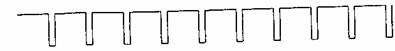
\includegraphics[scale=0.6]{figures/fig-4.jpg}

В Лондоне улицы извиваются, как им вздумается, и распределение импульсов выглядит случайным: иногда они сменяются часто, иногда редко.

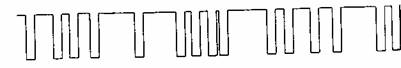
\includegraphics[scale=0.6]{figures/fig-5.jpg}

Ученый, которому показали бы эти меандры, вероятно, отчаялся бы отыскать в них какую нибудь закономерность; больше всего они походили бы на случайную последовательность, определяемую космическими лучами или распадом радиоактивного изотопа.

Другое дело, если этот ученый мыслил бы широко и оригинально.

Широты охвата можно достичь, поместив зеленую лампочку на голову каждого пешехода в Лондоне и записывая траектории в течение нескольких ночей. В результате получится толстая кипа миллиметровки с графиками, каждый из которых будет казаться совершенно случайным. Чем толще кипа, тем шире охват.

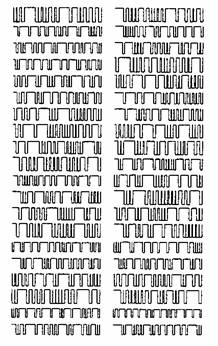
\includegraphics[scale=0.8]{figures/fig-6.jpg}

Оригинальность ума --- отдельное дело. Никто не знает, в чем тут финт. Один посмотрит на кипу меандров и не увидит ничего, кроме шума. Другой ощутит странный трепет, не понятный тому, кто подобного не испытывал. Некий глубинный отдел мозга, настроенный на поиск закономерностей (или наличия закономерностей), проснется и прикажет тупой будничной части мозга смотреть на кипу миллиметровки. Сигнал слабый и не всегда осмысленный, но человек просиживает сутками, перебирая кипу бумаг, как аутист, расстилает их по полу, сортирует на кучки по некой неведомой системе, подписывает цифирки и буквы мертвых алфавитов, рисует стрелки, ищет похожие места, сопоставляет их между собой.

Однажды этот человек выйдет из кабинета с подробной картой Лондона, восстановленной по графикам прямоугольных импульсов.

Лоуренс Притчард Уотерхауз --- один из таких людей.

Вот почему правительство его страны --- Соединенных Штатов Америки --- заставило Уотерхауза принести длиннейшую клятву секретности, исправно снабжало его обмундированием различных званий и родов войск, а теперь отправило в Лондон.

Он сходит с тротуара, рефлекторно смотрит налево. В правом ухе звон, визг мотоциклетных тормозов. Это всего лишь британский морской пехотинец на мотоцикле (Уотерхауз уже немного разбирается в знаках отличия), но за ним подкрепление --- защитного цвета фургон с написанными по трафарету кодовыми номерами.

--- Прошу прощения, сэр! --- бодро говорит морской пехотинец и объезжает Уотерхауза, видимо, сообразив, что с задачей додавить союзника вполне справится фургон. Уотерхауз прыгает вперед, прямо под колеса несущегося с другой стороны черного такси.

Впрочем, последний отрезок пути от этой конкретной улицы до Вестминстера он преодолевает без риска для жизни, если не считать близости к хорошо организованной орде немцев, оснащенной лучшими в мире средствами массового уничтожения. Эта часть города похожа на некоторые плохо освещенные закутки Манхэттена. Вдоль узких улочек тянутся десятиэтажные здания. Иногда Уотерхауз видит в просветы между домами впечатляющие готические громады и осознает близость Величия. Как и на Манхэттене, все куда то деловито спешат.

По военному времени каблуки у пешеходов подкованы, металлические набойки звякают на ходу. У каждого прохожего --- примерно постоянная длина шага, он вызвякивает на ходу с точностью метронома. Закрепив микрофон в бровке, шпион мог бы записать какофонию звяканий, случайную на первый взгляд, как писк из счетчика Гейгера. Однако правильный человек способен извлечь сигнал из шума --- вычислить соотношение мужчин и женщин, построить гистограмму длины ног...

Надо выбросить все это из головы и сосредоточиться на деле, которое пока еще скрыто мраком.

Над входом в станцию метро Сент Джеймс Парк сидит угловатая современная скульптура. Двадцать четыре часа в сутки она наблюдает за Бродвей билдингс. Как все штабы разведки, которые видел Уотерхауз, здание страшно разочаровывает.

Это в конечном счете всего лишь здание --- примерно десять этажей, сложенных из рыжего камня (три верхних составляет непомерно высокая мансарда), чуточка классического орнамента над окнами. Как все окна в Лондоне, они разделены клейкой лентой на восемь прямоугольных треугольников. Уотерхауз находит, что с классической архитектурой это согласуется лучше, чем, скажем, с готикой.

Он изучал физику и не верит, что от ударной волны, когда по соседству взорвутся несколько сот фунтов тринитротолуола, спасет клейкая лента. Скорее это суеверие, круги от сглаза на голландских коровниках в Пенсильвании. Может быть, вид ленты помогает людям сосредоточиться на войне.

На Уотерхауза это не действует. Он вдумчиво переходит улицу, думая о направлении движения, на случай, если из зданий за ним наблюдают. Входит, придерживает дверь стремительной девице в одежде военного покроя (которая всем своим видом показывает, что Уотерхауз ничего не добьется, просто подержав ей дверь), потом --- утомленному библейскому старцу с длинными седыми усами.

Вестибюль надежно охраняется. У Лоуренса долго проверяют документы. Затем он, естественно, поднимается не на тот этаж, потому что в Англии они нумеруются по другому. Все было бы куда смешнее, не происходи это в штабе военной разведки в разгар величайшей войны за всю историю человечества.

Нужный этаж, когда Уотерхауз наконец туда попадает, оказывается просто шикарным. Вообще в Англии шик во всем. Ничто не делается наполовину. Надо пройти милю, чтобы отыскать телефонную кабинку, зато уж выстроена она так, будто в недавнем прошлом немотивированный подрыв телефонных кабинок динамитом представлял собой реальную проблему для общества. А британский почтовый ящик, по всему, остановит немецкий танк. Ни у кого нет автомобиля, но уж если есть, так трехтонная махина ручной сборки. Идея, что можно штамповать машины на потоке, совершенно чужда здешнему сознанию: есть некий заведенный порядок, мистер Форд, которому надо следовать: ручная пайка радиаторов, выстругивание покрышек из цельного куска каучука и все прочее.

То же с официальными встречами. Уотерхауз всегда --- Гость; ему еще ни разу не приходилось принимать людей у себя. Гость прибывает в незнакомое здание, сидит в приемной; миловидная, но неприступная особа женского пола предлагает кофеинсодержащий напиток, от которого положено отказаться, потом проводит его в Кабинет, где сидят Главный и Остальные. Знакомят по некоторой системе, в которой Гостю разбираться не обязательно, поскольку он функционирует в пассивном режиме и должен лишь отзываться на сигналы извне: пожимать протянутые руки, отказываться от кофеинсодержащих и (на этой стадии) алкогольных напитков, садиться, где и когда скажут. В данном случае Главный и все Остальные, кроме одного --- британцы, выбор напитков слегка иной, Кабинет сложен из массивных глыб, как внутренняя гробница фараона, окна заклеены обычной неубедительной лентой. Фаза Предсказуемого Юмора короче, чем в Америке, фаза Светского Трепа --- длиннее.

Уотерхауз перезабывал все их фамилии. Он всегда с ходу забывает фамилии, а даже если бы не забыл, они ничего ему не говорят, потому что перед ним не положили организационные схемы Министерства иностранных дел (которое ведает разведкой) и Военного ведомства. Все постоянно говорят <<Вот и Хайс!>>, и когда он уже готов озираться в поисках Хайса, до него внезапно доходит, что так они произносят <<Уотерхауз>>. Кроме того, в его мозг проникает только одна ремарка --- когда кто то из Остальных говорит о премьер министре тоном, предполагающим короткое знакомство. А это даже не Главный. Главный гораздо старше и внушительнее. Поэтому Уотерхауз (хотя давно перестал слушать) остается под впечатлением, что по меньшей мере половина присутствующих недавно общались с Уинстоном Черчиллем.

Потом внезапно в разговоре мелькает определенное слово. Уотерхауз не слушал, но почти уверен, что в последние десять секунд кто то сказал: <<Ультра>>. Он моргает и выпрямляется.

Главный поднимает брови. Остальные озадачены.

--- Кажется, несколько минут назад что то говорили про кофе? --- спрашивает Уотерхауз.

--- Мисс Стенхоуп, кофе капитану <<Вот и Хайсу>>, --- говорит Главный в металлический селектор. Это один из полудюжины учрежденческих селекторов в Британской империи, зато цельнолитой, чугунный, весит сто фунтов и подсоединен к розетке с напряжением 420 вольт проводами толщиною в указательный палец. --- И будьте так любезны принести чай.

Теперь Уотерхауз знает, как зовут секретаршу Главного. Что ж, это зацепка. Отталкиваясь от нее, он сможет путем разысканий восстановить фамилию Главного.

Судя по всему, это вернуло их в фазу Светской Болтовни. Американские боссы были бы раздосадованы, британцы же, напротив, демонстрируют явное облегчение. Мисс Стенхоуп просят принести и другие напитки.

--- Вы в последнее время видели доктора Шеэна? --- спрашивает Уотерхауза Главный с ноткой тревожной заботы в голосе.

--- Кого? --- Тут Уотерхауз понимает, что речь о каперанге Шойне, и что в Лондоне его имя произносят более правильно.

--- Капитан Уотерхауз? --- спрашивает Главный через несколько минут. Уотерхауз придумывает новую криптографическую систему, основанную на разном произношении слов, и довольно долго не произносит ни слова.

--- Ах да! Я заскочил к нему перед отъездом. Конечно, когда он... э э... малость не того, с ним запрещено говорить о шифрах.

--- Разумеется.

--- Беда в том, что, когда у тебя с человеком все общие дела насчет криптологии, трудно удержаться и не нарушить приказ.

--- Да, весьма затруднительная ситуация.

--- Мне кажется, он более менее ничего. --- Уотерхауз говорит не очень убежденно. В кабинете наступает приличествующая тишина.

--- Когда он находился в более благоприятном состоянии, он восторженно писал о вашей работе над <<Криптономиконом>>, --- говорит один из Других, до сих пор по большей части молчавший. Уотерхауз решает, что это какая то шишка в мире машинной криптологии.

--- Мировой дядька, --- говорит Уотерхауз. Главный использует это как отправную точку.

--- Поскольку вы работали с машинами доктора Шойна, то входите в список <<Мэджик>>. Теперь, когда наши страны договорились --- по крайней мере в принципе --- сотрудничать в области криптологии, это автоматически включает вас в список <<Ультра>>.

--- Понятно, сэр, --- говорит Уотерхауз.

--- <<Ультра>> и <<Мэджик>> в значительной степени симметричны. В обоих случаях вражеская держава разработала шифр, который считает абсолютно невзламываемым. В обоих случаях союзная держава взломала шифр. В Америке доктор Шойн и его команда раскололи <<Индиго>> и построили машину <<Мэджик>>. У нас команда доктора Нокса взломала <<Энигму>> и построила <<Бомбу>>. Здесь светилом был доктор Тьюринг, у вас --- доктор Шойн, но он, как вы выразились, малость не того. Однако он утверждал, что вы вполне на уровне Тьюринга.

--- Чертовское преувеличение, --- говорит Уотерхауз.

--- Вы учились с доктором Тьюрингом в Принстоне, так?

--- Мы были там в одно время, если вы меня понимаете. Катались на велосипедах. Нас нечего сравнивать.

--- Но ведь доктор Тьюринг учился в аспирантуре, а вы были простым второкурсником.

--- Конечно. И все равно он гораздо сильнее меня.

--- Вы чересчур скромны, капитан Уотерхауз. Многие ли студенты публикуют статьи в международных журналах?

--- Мы просто катались на велосипедах, --- упрямо повторяет Уотерхауз. --- Эйнштейн даже говорить со мной не захотел.

--- Доктор Тьюринг всерьез занимался теорией информации, --- произносит не по годам изможденный тип с длинными седыми патлами. Уотерхауз мысленно определяет его как оксфордского профессора. --- Вероятно, вы обсуждали с ним эти темы.

Профессор поворачивается к остальным и говорит профессорским тоном:

--- Теория информации для механического калькулятора то же, что гидродинамика --- для корабельного корпуса. --- Потом оборачивается к Уотерхаузу и произносит чуть менее напыщенно: --- Доктор Тьюринг продолжал работать в этом направлении после того, как исчез с вашего горизонта и вступил в область Засекреченного. В особенности его интересовало, сколько именно информации можно извлечь из случайных, на первый взгляд, данных.

Внезапно все в кабинете вновь обмениваются удовлетворенными взглядами.

--- По вашей реакции я заключаю, --- говорит Главный, --- что и вы продолжали думать в этом же направлении.

Уотерхаузу интересно, какой была его реакция. Он отрастил клыки? Напустил слюней в кофе?

--- Это хорошо, --- говорит Главный раньше, чем Уотерхауз успевает ответить, --- потому что нам это тоже в высшей степени интересно. Понимаете, сейчас, когда мы прилагаем усилия --- подчеркну, предварительные и явно недостаточные усилия скоординировать действия американской и британской разведки, мы оказываемся в нелепейшей ситуации. Мы знаем все, капитан Уотерхауз. Мы читаем личные послания Гитлера военачальникам на местах зачастую раньше самих военачальников. Очевидно, что такое знание --- мощнейшее оружие. Но так же очевидно, что оно не поможет выиграть войну, если мы не будем действовать в соответствии с полученным знанием. То есть если с помощью <<Ультра>> мы узнали, что из Таранто в Северную Африку вышел конвой с припасами для Роммеля, это знание бесполезно, если мы не потопим конвой.

--- Ясно, --- говорит Уотерхауз.

--- Теперь, если десять конвоев вышли и все потоплены, даже те, что двигались ночью или в тумане, немцы спросят себя, как мы их нашли. Они поймут, что мы раскрыли шифр <<Энигма>>, сменят его, и это оружие будет для нас утрачено. Смело могу сказать, что мистера Черчилля огорчит такой поворот событий.

Главный смотрит на Остальных, те важно кивают. У капитана Уотерхауза такое впечатление, что мистер Черчилль относится к этому вопросу весьма серьезно.

--- Давайте изложим суть дела в терминах теории информации, --- говорит профессор. --- Информация течет к нам из Германии через систему <<Ультра>> в Блетчли парке. Информация поступает туда в виде случайных на первый взгляд сигналов азбуки Морзе, которые передаются по радио. Но поскольку у нас есть очень умные люди, способные отыскать смысл во внешне случайной последовательности, мы получаем чрезвычайно важную информацию. Так вот, немцы пока не взломали наши главные шифры. Однако они могут наблюдать за нашими действиями --- за маршрутами наших конвоев в Северной Атлантике, за перемещениями самолетов. Если конвои всякий раз обходят стороной немецкие подводные лодки, а наши бомбардировщики летят прямиком к немецким конвоям, то немец --- я говорю об очень умном немце, о немце ученом --- понимает, что тут действует не случайность. Этот немец может отыскать корреляцию. Он увидит, что мы знаем больше, чем должны бы. Другими словами, с какого то момента информация начинает течь от нас к немцам.

--- Мы должны знать, где этот момент, --- произносит Главный. --- Знать точно. Чтобы создать впечатление случайности.

--- Да, --- говорит Уотерхауз, --- и это должна быть такая случайность, чтобы обмануть кого нибудь вроде Рудольфа фон Хакльгебера.

--- Именно его мы и имели в виду, --- подхватывает профессор. --- Доктора фон Хакльгебера, с прошлого года.

--- Ой! --- радостно восклицает Уотерхауз. --- Руди защитился?

Поскольку Руди призвали назад в объятия Тысячелетнего Рейха, Уотерхауз предполагал худшее: Руди в шинели, спит в сугробе где нибудь под Ленинградом или вроде того. Однако, выходит, фашисты, способные ценить ум (если только этот ум --- не еврейский), нашли ему кабинетную работу.

Наступает неловкое молчание. Кто то из Других, пытаясь разрядить обстановку, шутит, что, если бы Руди догадались задержать в Нью Джерси, не потребовалось бы вводить гриф секретности <<Ультра Мега>>. Никто не смеется, и Уотерхауз заключает, что дело обстоит именно так.

Ему показывают схему организации специального подразделения №2701 ВВС Британии, куда включены все двадцать четыре человека в мире, допущенные к <<Ультра Мега>>. Верх украшают такие люди, как Уинстон Черчилль и Франклин Делано Рузвельт. Затем идут фамилии, которые кажутся Уотерхаузу смутно знакомыми: может быть, это как раз те, с кем он сейчас разговаривает. Под ними --- некий Чаттан, молодой полковник британских ВВС, отличившийся (объясняют Уотерхаузу) в Битве за Британию.

На следующем уровне списка --- Лоуренс Притчард Уотерхауз и две другие фамилии: капитан ВВС Британии и капитан МПФ США. Вбок отходит пунктирная линия к Алану Матисону Тьюрингу. В целом это, похоже, самое невероятное собрание людей, когда либо возникавшее в недрах военной организации. В самом низу схемы располагаются две колонки по шесть фамилий, расположенные под капитанами британских ВВС и американской морской пехоты соответственно. Исполнительное крыло организации: как говорит один из сидящих в кабинете, <<люди в забое>>, или, как поясняет Уотерхаузу единственный американец, <<это там, где покрышка соприкасается с шоссе>>.

--- Вопросы есть? --- спрашивает Главный.

--- Число выбрал Алан?

--- Вы имеете в виду доктора Тьюринга?

--- Да. Это он выбрал число 2701?

Такие детали явно на несколько уровней ниже статуса людей в Бродвей билдингс. Они удивлены и немного оскорблены, как будто Уотерхауз попросил их написать под диктовку.

--- Возможно, --- говорит Главный. --- Почему вы спросили?

--- Потому что, --- отвечает Уотерхауз, --- 2701 это произведение двух простых чисел, 37 и 73, которые, будучи записаны в десятичной системе, представляют собой, как вы легко можете видеть, взаимную перестановку цифр.

Все лица обращаются к ученому, который явно пристыжен.

--- Это лучше исправить, потому что именно такие вещи может заметить Рудольф фон Хакльгебер. --- Он встает, вынимает из кармана авторучку с золотым пером и переправляют 2701 на 2702. Уотерхауз оглядывает собравшихся и приходит к выводу, что все довольны. Очевидно, именно таких салонных фокусов от него и ждут.


\chapter{КОРРЕХИДОР}


В Манильской бухте нет четкой границы между водой и влажным воздухом, только голубовато серая пелена. <<Глория IV>> с полчаса осторожно маневрирует между стоящими на якоре грузовыми судами, потом набирает скорость и устремляется к середине залива. Дымка немного рассеивается, Рэнди хорошо видит по правому борту Батаан: черные горы, по большей части окутанные мглой и испещренные облачными грибами восходящих термальных потоков. Пляжей почти нет, красные склоны обрываются к воде. По мере того как катер огибает полуостров, берег становится положе, видны зеленые луга. На самом конце полуострова --- два известняковых утеса, которые Рэнди помнит по кассете Ави. Однако взгляд его прикован к Коррехидору в нескольких милях от полуострова.

Америка Шафто, или Ами, как она предпочитает зваться, большую часть времени проводит вне каюты, оживленно разговаривает с филиппинцами и американцами или сидит по турецки на палубе, перебирает карты и бумаги. Она надела ковбойскую соломенную шляпу от солнца. Рэнди не торопится подставлять себя прямым лучам: бродит по каюте, потягивает кофе, рассматривает фотографии.

Он наивно ожидал увидеть много снимков, на которых водолазы укладывают кабель. <<Семпер марин сервисис>> прокладывают много кабеля, и прокладывают хорошо, Рэнди наводил справки, прежде чем заключить контракт. Однако, видимо, здесь не считают, что такую работу интересно снимать. На большей части фотографий --- поиск затонувших сокровищ: ныряльщики, широко улыбаясь, демонстрируют облепленные ракушками вазы, словно хоккеисты --- Кубок Стэнли.

Коррехидор с этого расстояния --- выступающая из воды чечевица джунглей с тянущимся в одну сторону шельфом. Рэнди видел карты и знает, что на самом деле остров имеет форму сперматозоида. То, что отсюда кажется шельфом, на самом деле --- хвост, который извивается к востоку, как будто сперматозоид хочет выплыть из Манильского залива, чтобы оплодотворить Азию.

Пробегает Ами, распахивает дверь каюты.

--- Идемте в рубку, --- говорит она, --- посмотрите.

Рэнди идет за ней.

--- Кто это на большинстве фотографий? --- спрашивает он.

--- В шрамах, с <<ежиком>>?

--- Да.

--- Мой отец. Дуг.

--- Дуглас Макартур Шафто? --- спрашивает Рэнди. Он видел это имя на контракте с <<Семпер марин>>.

--- Он самый.

--- Бывший <<Морской лев>>\footnote{<<Морские львы>> --- подразделения сил специальных операций ВМС США, предназначенные для ведения разведки и диверсионных операций в портах на морском и речном побережье.}?

--- Ага. Только он не любит, когда так говорят. Уж очень заезженно.

--- Почему его имя и фамилия кажутся мне знакомыми?

Ами вздыхает.

--- Он получил свои пятнадцать минут славы в тысяча девятьсот семьдесят пятом.

--- Не могу вспомнить.

--- Комстока знаете?

--- Генерального прокурора Пола Комстока? Врага криптографии?

--- Я про его отца, Эрла Комстока.

--- Идеолога холодной войны? Организатора войны во Вьетнаме?

--- Никогда не слышала, чтобы его так называли, но да, мы говорим об одном человеке. Может быть, вы помните, что в тысяча девятьсот семьдесят пятом Эрл Комсток выпал, или был вытолкнут, из горнолыжного подъемника в Колорадо и сломал руку.

--- Ах да. Вроде вспоминается.

--- Отец... --- Ами кивает на одну из фотографий, --- был на соседнем сиденье.

--- Случайно или...

--- Чисто случайно. Не преднамеренно.

--- Это с какой стороны посмотреть, --- говорит Рэнди. --- Если Эрл Комсток часто катался на лыжах, довольно велика вероятность, что рано или поздно он оказался бы в пятидесяти футах над землей рядом с ветераном вьетнамцем.

--- Без разницы. Я просто хочу сказать, что мне неохота об этом говорить.

--- Я с ним познакомлюсь? --- спрашивает Рэнди, глядя на фотографию.

Ами закусывает губу и смотрит на горизонт.

--- В девяноста процентах случаев его присутствие на борту означает, что происходит нечто необычное. --- Она открывает люк и, придерживая крышку, показывает Рэнди на высокие ступеньки.

--- А остальные десять?

--- Ему скучно или он поссорился с подружкой.

Рулевой <<Глории>> занят своим делом и не обращает на них внимания, что Рэнди воспринимает как знак профессионализма. В рубке множество самодельных столов из толстой фанеры или старых дверей, все свободное место занято электроникой: здесь есть факс, машинка поменьше, выдающая сводки погоды, три компьютера, спутниковый телефон, несколько радиотелефонов на базах для подзарядки, эхолот и другие гидроакустические приборы. Ами подводит Рэнди к большому экрану, на котором что то вроде черно белого фото гористой местности. <<Локатор бокового обзора, --- объясняет она. --- Незаменимая вещь для такого рода работы. Показывает, что на дне>>.

Ами смотрит на одном из компьютеров текущие координаты и что то быстро прикидывает в уме.

--- Эрнесто, пять градусов вправо, пожалуйста.

--- Есть, мэм, --- говорит Эрнесто и поворачивает на пять градусов вправо.

--- Что вы ищете?

--- Бесплатное приложение, --- объясняет Ами. --- Маленький бонус для наших клиентов --- экскурсия с показом достопримечательностей. Видите? Вот. --- Она мизинцем показывает что то, секунду назад возникшее на экране.

Рэнди нагибается и всматривается. Явно антропогенное образование: мешанина прямых углов и прямых линий.

--- Похоже на груду обломков.

--- Так и есть, --- отвечает Ами. --- Когда то это была значительная часть филиппинского национального достояния.

--- Что?!

--- Во время войны, --- говорит Ами, --- после Перл Харбора, но до того, как японцы заняли Манилу, правительство опустошило казну. Все золото и серебро упаковали в ящики и вывезли на Коррехидор --- якобы для сохранности.

--- Что значит <<якобы>>?

Ами пожимает плечами.

--- Это Филиппины. У меня такое чувство, что определенная часть ушла на сторону. Однако много серебра оказалось здесь. --- Она выпрямляется и кивает на Коррехидор за окном. --- Тогда считалось, что Коррехидор неприступен.

--- Когда примерно?

--- В декабре сорок первого --- январе сорок второго. Так или иначе, скоро стало ясно, что Коррехидор падет. В начале февраля одна подводная лодка забрала золото, вторая --- людей, которых нельзя было оставлять неприятелю, вроде дешифровщиков. На серебро подлодок не хватило. Макартур оставил Филиппины в марте. Ящики с серебром выносили ночью и бросали в море.

--- Вы меня подкалываете?

--- Лучше утопить, чем оставить японцам, правда?

--- Да, наверное.

--- Японцы подняли значительную часть серебра. Они взяли в плен американских водолазов на Батаане и Коррехидоре и заставили их работать. Однако пленные ухитрялись припрятать часть серебра и передать филиппинцам, которые тайком доставляли его в Манилу. Серебра было столько, что оно совершенно подорвало японские оккупационные деньги.

--- Так что мы видим сейчас?

--- Остатки ящиков, развалившихся от удара о дно, --- говорит Ами.

--- А после войны серебро еще оставалось?

--- Конечно, --- легко отвечает Ами. --- Большую часть сбросили сюда, и его подняли водолазы, но что то вывалили в других местах. Одно такое место отец нашел в семидесятых.

--- Обалдеть! Ерунда какая то.

--- А что?

--- Не поверю, что груды серебра так и лежат тридцать лет бери, кто хочет.

--- Вы плохо знаете Филиппины, --- говорит Ами.

--- Я знаю, что это бедная страна. Почему бы не поднять серебро?

--- Большая часть охотников за сокровищами в этой часта мира ищет добычу покрупнее, --- говорит Ами, --- или полегче.

Рэнди не унимается.

--- По моему, груда серебра на дне бухты --- достаточно крупная и легкая добыча.

--- Вовсе нет. Серебро не так дорого стоит. Ваза династии Сун, если ее поднять и очистить от ракушек, стоит дороже золота. Золота! А найти ее много легче --- просто прощупываешь дно эхолотом. Затонувший корабль дает на экране характерную картинку. А старый ящик, разбитый, поросший кораллами и ракушками, больше всего похож на камень.

По мере того как они приближаются к Коррехидору, Рэнди видит, что хвост у острова корявый, из него там и сям торчат нагромождения каменных глыб. От толстой оконечности острова к кончику хвоста темная зелень джунглей постепенно сменяется более светлой растительностью, затем --- красновато бурой сухой почвой. Рэнди смотрит на один из скалистых выступов, который теперь венчает рупорная антенна, повернутая на восток, к зданию корпорации <<Эпифит>> в Интрамурос.

--- Видите пещеры сразу над водой? --- говорит Ами. Она, по всей видимости, жалеет, что завела речь о сокровищах, и теперь хочет сменить тему.

Рэнди с сожалением отводит взгляд от антенны, которой частично владеет, и смотрит туда, куда указывает девушка. Известняковый бок острова, круто уходящий в воду, изъеден дырами.

--- Ага.

--- Их пробили американцы для береговых орудий. Японцы расширили, и там помещались лодки камикадзе.

--- Обалдеть.

Рэнди слышит низкий горловой звук и, переведя взгляд, видит, что с ними поравнялась лодка. Она узкая и длинная, как каноэ, с балансирами по обоим бортам. На короткой мачте развеваются два флага; повсюду протянуты веревки, на них весело хлопает разноцветное постиранное белье. Посредине большой дизель без кожуха отравляет атмосферу клубами черного дыма. Ближе к носу несколько филиппинцев, включая женщин и детей, перекусывают под ярко голубым тентом. На корме двое возятся с водолазным снаряжением. Один что то держит у рта: микрофон. Рация на <<Глории>> хрипит по тагальски. Эрнесто подавляет смешок, берет микрофон, коротко отвечает. Очевидно, это что нибудь вроде: <<Потом потреплемся. У нас в рубке клиент>>.

--- Коллеги, --- сухо поясняет Ами. По всему видно, что ей хочется отделаться от Рэнди и вернуться к работе.

--- Спасибо за экскурсию, --- говорит Рэнди. --- Один вопрос.

Ами поднимает брови, стараясь выглядеть спокойной.

--- Какую часть доходов <<Семпер марин>> дает охота за сокровищами?

--- В этом месяце? В этом году? За десять лет? За все время существования фирмы?

--- Без разницы.

--- Год на год не приходится, --- отвечает Ами. --- Мы окупили <<Глорию>> и еще немного заработали вазами с затонувшего корабля. Но в иные годы весь доход давала работа, как эта.

--- Другими словами, скучная работа, от которой тошнит? --- спрашивает Рэнди. Выпаливает, не подумав. В нормальных обстоятельствах он лучше контролирует свои слова. Однако борода сбрита, границы <<я>> разрушены или что то в таком роде.

Он думает, что Ами рассмеется или хотя бы подмигнет, но она воспринимает его слова совершенно серьезно. У нее классно получается каменное лицо.

--- Смотрите на это как на клепку номерных знаков.

--- Значит, на самом деле вы --- охотники за сокровищами, --- подводит итог Рэнди. --- А номерные знаки клепаете, чтобы иметь приток денежных средств.

--- Зовите нас охотниками за сокровищами, если хотите. Зачем вы пошли в бизнес, Рэнди? --- Она поворачивается и выходит.

Рэнди смотрит ей вслед. Эрнесто тихо чертыхается, не столько со зла, сколько от изумления. <<Глория>> как раз огибает хвост Коррехидора, и становится видна вся южная сторона острова. На протяжении последней полумили хвост изгибается, образуя полукруглую бухту. В середине бухты стоит белый корабль, который Рэнди поначалу принимает за океанский лайнер с жесткими, разбойничьими обводами. Потом он видит на корме название и порт приписки: <<РУИ ФАЛЕЙРО --- САНТА МОНИКА, КАЛИФОРНИЯ>>.

Рэнди подходит к Эрнесто, и они некоторое время вместе глядят на яхту. Рэнди о ней слышал, а Эрнесто, как все на Филиппинах, давно знает. Однако увидеть се своими глазами --- совершенно другое дело. На юте, как игрушечка, стоит вертолет. На шлюпбалке кинжалом качается мощный гоночный катер, который в любую минуту можно спустить на воду. Смуглолицый мужчина в ослепительно белой форме драит медный поручень.

--- Руи Фалейро был космографом Магеллана, --- говорит Рэнди.

--- Космографом?

--- Мозгом операции. --- Рэнди стучит себя по голове.

--- Он приплыл сюда с Магелланом? --- спрашивает Эрнесто.

Для всего остального мира Магеллан --- человек, совершивший первое кругосветное плавание. Здесь каждому известно, что добрался он только до острова Мактан, где был убит филиппинцами.

--- Когда Магеллан вышел в море, Фалейро остался в Севилье, --- говорит Рэнди. --- Он сошел с ума.

--- Вы много знаете про Магеллана, да? --- спрашивает Эрнесто.

--- Нет, --- отвечает Рэнди. --- Я много знаю про Дантиста.


--- Не разговаривай с Дантистом. Никогда. Ни о чем. Даже о технической стороне. Любой его технический вопрос --- всего лишь пробный шар в деловой стратегии, до которой тебе --- как Даффи Даку до теоремы Геделя.

Ави огорошил этим Рэнди однажды вечером, когда они обедали в ресторане в центре Макати. Ави отказывается говорить о чем нибудь серьезном в радиусе мили от гостиницы <<Манила>>; он убежден, что каждый номер и каждый столик прослушиваются.

--- Спасибо за доверие, --- сказал Рэнди.

--- Пойми, --- ответил Ави, --- я просто пытаюсь застолбить территорию --- оправдать свое участие в проекте. Деловой стороной буду заниматься я.

--- У тебя, часом, не мания преследования?

--- Слушай сюда. У Дантиста примерно миллиард долларов своих и еще десять миллиардов под управлением. Все вонючие ортодонты в Южной Калифорнии ушли на пенсию в сорок лет, потому что Дантист за два или три года удесятерил их индивидуальные пенсионные счета. Хорошим людям деньги сами не плывут.

--- Может, ему просто везло.

--- Везло, да. Но это еще не значит, что он хороший человек. Я о том, что он инвестирует в крайне рискованные предприятия. Он играет в русскую рулетку на пенсионные сбережения вкладчиков, не ставя их в известность. Он вложил бы деньги в исламистов с Минданао, если бы считал, что захват заложников принесет хорошие дивиденды.

--- Интересно, он понимает, что ему везло?

--- Мне тоже интересно. Думаю, нет. Думаю, он считает себя орудием Божественного Провидения, как Дуглас Макартур.


<<Руи Фалейро>> --- гордость быстроразвивающегося сиэтлского суперъяхтостроения. Рэнди почерпнул кое какие сведения о яхте из рекламного буклета, выпущенного еще до того, как Дантист ее купил. Поэтому он знает, что вертолет и гоночный катер входили в сумму сделки, которая не разглашается. В убранстве яхты использовано, помимо всего прочего, десять тонн мрамора. В хозяйских каютах две уборные, М и Ж, отделанные соответственно черным и розовым мрамором, чтобы Дантист и Дива не толклись у одной раковины, готовясь к большому приему в бальном помещении яхты.

--- Про Дантиста? --- переспрашивает Эрнесто.

--- Про Кеплера. Доктора Кеплера, --- говорит Рэнди. --- В Штатах некоторые люди называют его Дантистом. Люди, занятые в сфере высоких технологий. Эрнесто понимающе кивает.

--- Такой человек мог выбрать себе любую женщину в мире, --- говорит Эрнесто, --- но он выбрал филиппинку.

--- Да, --- осторожно соглашается Рэнди.

--- А в Штатах знают историю жизни Виктории Виго?

--- Должен признаться, в Штатах она не так известна, как на Филиппинах.

--- Конечно.

--- Хотя некоторые ее песни очень популярны. Многим известно, что она выбилась из нищеты.

--- А в Штатах знают про Дымную Горку? Про свалку в Тондо, где дети ищут себе еду?

--- Некоторые --- да. Еще больше узнают, когда фильм про Викторию Виго покажут по телевизору.

Эрнесто удовлетворенно кивает. Здесь всем известно, что выходит фильм про жизнь Дивы с ней самой в главной роли. Однако мало кто в курсе, что фильм заведомо убыточный, снимается на деньги Дантиста и пройдет по кабельному каналу в ночные часы.

Зато, наверное, все понимают, что самого интересного там не будет.


--- В том, что касается Дантиста, --- сказал Ави, --- утешает одно. На Филиппинах он будет совершенно предсказуемый. Ручной. Даже смирный.

--- Это почему?

--- Виктория Виго --- бывшая проститутка, верно?

--- Ну, люди перемигиваются и толкают друг друга в бок по этому поводу, но я впервые слышу, чтобы такое сказали вслух, --- ответил Рэнди, нервно озираясь.

--- Поверь, с Дымной Горки другого пути нет. Проституцией здесь заправляют Болоболо --- группа с Северного Лусона, которая пришла к власти вместе с Маркосом. Они контролируют эту сферу жизни: полицию, организованную преступность, местную политику, все такое. Соответственно Виктория Виго на крючке: у них есть фотографии и видеозаписи с тех времен, когда она была малолетней проституткой и снималась в порно.

Рэнди изумленно брезгливо помотал головой.

--- Откуда, черт возьми, ты это все знаешь?

--- Не важно. Поверь мне, в определенных кругах это известно не хуже, чем значение числа <<$\pi$>>.

--- Только не в моих.

--- Так или иначе, ее интересы связаны и всегда будут связаны с Болоболо. А Дантист будет послушно выполнять все, что скажет жена.

--- Ты уверен? --- усомнился Рэнди. --- Он --- акула бизнеса. Денег и влияния у него, вероятно, побольше, чем у Болоболо. Он волен поступать, как ему вздумается.

--- Но не будет, --- заявил Ави с полуулыбкой. --- Он поступит так, как велит жена.

--- Откуда ты знаешь?

--- Послушай, --- сказал Ави. --- Кеплер, как большинство богатых, влиятельных людей, одержим властью, верно?

--- Верно.

--- Если ты настолько одержим властью, в какие сексуальные предпочтения это должно вылиться?

--- Надеюсь никогда не узнать. Наверное, я хотел бы подавлять женщину.

--- А вот и нет! --- сказал Ави. --- Секс гораздо сложнее, Рэнди. Секс --- это то, где вылезают наружу подавленные желания. Люди сильнее всего заводятся, когда обнажаются их самые глубинные тайны...

--- Черт! Кеплер --- мазохист?

--- Он такой гребаный мазохист, что прославился своим мазохизмом. По крайней мере, в восточноазиатской секс индустрии. Сутенеры и хозяйки борделей в Гонконге, Бангкоке, Шенжене, Маниле --- все имеют на него досье и точно знают, что ему нужно. Так он и познакомился с Викторией Виго. Он был в Маниле, прорабатывал сделку с <<ФилиТел>>. Жил в отеле, которым владеют и который прослушивают Болоболо. Они изучали его случки, как энтомологи изучают спаривание муравьев. Они запрограммировали Викторию Виго --- свою козырную карту, свою бомбу, своего сексуального Терминатора, --- чтобы дать в точности то, что он хочет, потом направили в его жизнь, как ракету точного наведения, и бац! --- истинная любовь.

--- И он ничего не заподозрил? Меня удивляет, что он настолько увлекся шлюхой.

--- Он не знал, что она шлюха. В этом то вся красота плана! Болоболо подсадили ее консьержкой ему в отель! Скромную католическую школьницу! Началось с того, что она заказывала Кеплеру билеты в театр, а через год он лежит на своей гребаной мегаяхте с исполосованной задницей, прикованный наручниками к кровати, а она стоит рядом, и на пальце у нее обручальное кольцо размером с автомобильную фару --- сто тридцать восьмая в списке самых богатых женщин планеты!

--- Сто двадцать пятая, --- поправил его Рэнди. --- Акции <<ФилиТел>> недавно пошли вверх.


Следующие несколько дней Рэнди проводит, стараясь не столкнуться с Дантистом. Он остановился в маленькой частной гостинице на вершине острова, каждое утро пьет кофе с булочкой в компании американских и японских ветеранов. Они приехали сюда вместе с женами, чтобы (предполагает Рэнди) разобраться с чувствами, в миллион раз более глубокими, чем все, что когда либо доводилось испытывать ему самому. <<Руи Фалейро>> постоянно на виду, и Рэнди может определить, на борту ли Дантист, наблюдая за вертолетом и катером.

Когда он думает, что все безопасно, то идет на берег под УКВ антенной и смотрит, как водолазы Ами возятся с кабелем. Некоторые работают в прибрежной полосе, завинчивают вокруг кабеля секции металлических труб. Другие --- милях в двух от берега, рядом с баржей, которая укладывает кабель непосредственно в илистый грунт с помощью исполинского приспособления, похожего на мясницкий нож.

Береговой отрезок кабеля тянется в новое железобетонное здание в ста метрах от верхней приливной отметки. Собственно, это одно большое помещение, набитое аккумуляторами, генераторами, кондиционерами и электронным оборудованием. За программы, которые на этом оборудовании крутятся, отвечает Рэнди, поэтому; он проводит большую часть времени в здании, глядя на монитор и стуча по клавиатуре. Отсюда тянутся провода к УКВ башне.

Другой конец кабеля уходит туда, где в Южно Китайском море качается на волнах буй. До него несколько километров. Буй отмечает конец Северо Лусонского Кабеля, принадлежащего компании <<ФилиТел>>. Если двигаться вдоль него, попадешь в здание на северной оконечности острова, куда подходит большой кабель с Тайваня. К Тайваню, в свою очередь, сходится целая подводная кабельная сеть. Передавать данные на Тайвань и с Тайваня просто и дешево.

В линии передачи, которой <<Эпифит>> и <<ФилиТел>> пытаются связать Тайвань и Манилу, только один зазор, и он уменьшается день ото дня, по мере того как баржа смещается к бую.


Когда они наконец сходятся, <<Руи Фалейро>> поднимает якорь и движется к месту встречи. Вертолет, гоночный катер и флотилия нанятых лодок курсируют между яхтой и берегом, доставляя из Манилы важных людей и прессу. Появляется Ави с двумя смокингами из шанхайского ателье (<<Все знаменитые гонконгские портные --- беженцы из Шанхая>>). Они с Рэнди разрывают оберточную бумагу, облачаются и едут в джипе с кондиционером к пристани, где дожидается <<Глория>>.

Через два часа Рэнди впервые видит Дантиста и Диву в большом бальном зале <<Руи Фалейро>>. Для Рэнди это прием как прием --- он жмет людям руки, тут же забывает как их зовут, садится и в одиночестве принимается за еду и вино.

Единственное, что здесь необычно --- на шканцах лежат два кабеля, каждый толщиной с бейсбольную биту. Если подойти к фальшборту, можно увидеть, как их концы уходят в пучину. Противоположные концы сходятся на столе посреди палубы, где техник, доставленный самолетом из Гонконга и облаченный в смокинг, мается со стыковкой. Еще он мается с тяжелого бодуна, но Рэнди ничуть не встревожен: он знает, что все это исключительно для понта и оба куска кабеля заканчиваются в воде рядом с яхтой. Настоящее соединение выполнено вчера, кабель лежит на дне, и по нему уже бегут биты.

На шканцах еще один человек. Он смотрит на Батаан и Коррехидор, одновременно наблюдая за Рэнди. Поймав взгляд Рэнди, кивает, как будто мысленно сверился с каким то списком, встает и подходит. На нем парадная военная форма, флотский аналог смокинга. Он почти лыс, оставшаяся седина сострижена миллиметрах в пяти от головы. Когда он идет к Рэнди, несколько филиппинцев наблюдают за ним с явным любопытством.

--- Здравствуйте, Рэнди. --- Человек в форме жмет Рэнди руку, медали звякают друг о друга. На вид ему лет пятьдесят, но кожа --- как у восьмидесятилетнего бедуина. На груди множество ленточек, в основном красно желтых, что у Рэнди смутно ассоциируется с Вьетнамом. Над карманом пластиковая табличка: <<ШАФТО>>.

--- Не обманывайтесь, Рэнди, --- говорит Дуглас Макартур Шафто. --- Я не на действительной службе. Сто лет как в запасе. Однако форму имею право носить. И это гораздо проще, чем найти на меня смокинг.

--- Рад познакомиться.

--- Я тоже. Кстати, откуда ваш?

--- Смокинг?

--- Да.

--- Заказали.

--- Подруга?

--- Партнер. Я временно без подруги.

--- Значит, вы не обзавелись спутницей в Маниле. В отличие от нашего хозяина.

Рэнди смотрит в бальный зал на Викторию Виго. Если бы она сияла еще сильнее, со стен бы полезла краска, а подоконники начали оседать, как воск.

--- Наверное, я слишком стеснительный или вроде того, --- говорит Рэнди.

--- Стеснительность не помешает вам выслушать деловое предложение?

--- Отнюдь.

--- Моя дочь полагает, что вы и наш хозяин намерены в будущем проложить еще несколько кабелей.

--- В бизнесе редко что то делают один раз, --- говорит Рэнди. --- Это затрудняет бухгалтерию.

--- Вы уже знаете, что море здесь очень мелкое.

--- Да.

--- И знаете, что кабель нельзя прокладывать в мелкой воде без предварительной очень детальной локационной съемки морского дна.

--- Да.

--- Съемку хотел бы провести я.

--- Понятно.

--- Нет, не думаю, чтобы вам было понятно. Однако я хочу, чтобы вы поняли, поэтому объясню.

--- Хорошо, --- кивает Рэнди. --- Позвать партнера?

--- Идея, которую я намерен предложить, очень проста, и для ее восприятия не нужны два первоклассных специалиста.

--- Отлично. Что за идея?

--- Подробная съемка даст чертову уйму информации обо всем, что лежит па морском дне. Часть информации может оказаться ценной. Ценнее, чем вы ожидаете.

--- А, --- говорит Рэнди, --- вы хотите сказать, это может быть то, что ваша фирма умеет обращать в капитал.

--- Да, --- отвечает Дуг Шафто. --- Если вы наймете кого нибудь из моих конкурентов, они, наткнувшись на такую информацию, используют ее сами, а вам ничего не скажут. Вы не узнает об их находках и не получите прибыли. Если вы наймете <<Семпер марин сервисис>>, я буду сообщать обо всех находках. Вы и ваша фирма получите свою долю.

--- M м, --- тянет Рэнди. Он пытается сделать каменное лицо, но понимает, что Дуг Шафто видит его насквозь.

--- При одном условии, --- говорит Дуг Шафто.

--- Я подозревал, что будут условия.

--- Любая стоящая приманка насажена на крючок. Это крючок.

--- И в чем он состоит?

--- Ни слова этому козлу. --- Дуг Шафто поводит большим пальцем в сторону Хьюберта Кеплера. --- Потому что если Дантист разнюхает, они с Болоболо все приберут к рукам и нам ничего не достанется. Есть даже шанс, что нас просто убьют.

--- Ну, насчет <<просто убьют>> и впрямь стоит подумать, --- говорит Рэнди, --- но я передам партнеру ваше предложение.


\chapter{ТУННЕЛЬ}


Уотерхауз и несколько десятков незнакомцев стоят и сидят в необыкновенно узком, вытянутом помещении, которое раскачивается из стороны в сторону. В помещении длинный ряд окон, но свет через них не идет, только звук: грохот, дребезжание и скрежет. Все погружены в себя и молчат, как в церкви перед началом службы.

Уотерхауз стоит, держась за петлевидный отросток потолка, иначе полетит спиной. Последние две минуты он внимательно разглядывал плакат с инструкцией по надеванию противогаза. У него самого, как и у всех, противогаз с собой, в брезентовой сумке через плечо. Сумка, правда, не такая, как у всех, потому что она американская и военного образца. На нее косятся.

На плакате --- светлоликая модница с золотисто каштановыми волосами, которые явно химически размягчили и заново отформовали в дорогой парикмахерской. Стоит прямо, как по струнке, подбородок выставлен, локти согнуты, ладони сложены в ритуальном жесте: пальцы в стороны, большие --- вертикально вверх. На уровне лица в хитросплетении защитного цвета тесемок болтается жутковатый комок. Поднятые большие пальцы --- опорная конструкция тесемочной паутины.

Уотерхауз в Лондоне уже два дня и в курсе, что будет дальше. Он узнает эту позу где и когда угодно. Красавица изготовилась, чтобы сделать энергичное движение подбородком. Если столица подвергнется газовой атаке, верхушки массивных почтовых ящиков, покрытые специальной краской, почернеют и раздастся определенный сигнал. Двадцать миллионов больших пальцев взметнутся к ядовито зеленым, отравленным небесам. Десять миллионов противогазов повиснут в воздухе. Десять миллионов подбородков рывком вдвинутся в маску. Уотерхауз почти слышит скрип, с которым нежная кожа красавицы втискивается в тугую черную резину.

Как только подбородок всунут, все в порядке. Надо еще аккуратно распределить тесемки на золотисто каштановом перманенте и побыстрее добраться до закрытого помещения, но самое страшное позади. У британских противогазов впереди круглая плоская нашлепка, чтобы дышать, в точности как свиной пятачок. Ни одна женщина не согласилась бы, чтобы ее застали мертвой в такой штуке, если бы их не надевали на плакатах безупречные красавицы.

Что то мелькает в темноте за окном. Поезд едет в той части подземки, где брезжит тусклый свет, обнажая стигийские тайны метро. Все в вагоне моргают, переглядываются, вздыхают. Вокруг на мгновение вновь материализовался мир. Фрагменты стены, металлические балки, пучки кабеля небесными телами проплывают в пространстве по мере того, как поезд ползет мимо.

Уотерхауз смотрит на кабели. Они тянутся параллельно и прикреплены к стене металлическими скобами --- словно побеги некоего глубинного плюща, расползаются во мраке метро, тайком от обслуживающего персонала ищут, как бы пробиться наружу, к свету.

На улице, в Надземье, можно видеть, как первые цепкие усики карабкаются по древним стенам зданий. Неопреновые лианы, будто по отвесу, взбираются по вертикальной плоскости и проникают в дыры оконных рам, особенно тяготея к учреждениям, Иногда они заключены в трубы. Иногда хозяева их закрашивают Но у всех --- общая корневая система, которая идет по туннелям и щелям подземелья, сходясь к исполинским коммутаторам в глубоких бетонных бункерах.

Поезд врывается в храм грязновато желтого света, со стоном останавливается под сводами. Аляповатые иконы общенационального умопомешательства поблескивают в нишах и боковых приделах. Ангелоподобная женщина с противогазом --- на одном конце морального континуума. На противоположном --- дьяволица в узкой юбке посреди людной гостиной шпионски ухмыляется из под накладных ресниц, ловя неосторожные слова наивных молодых офицериков.

Табличка на стене внушающим доверие официальным рубленым шрифтом утверждает, что это Юстон. Уотерхауз и большая часть остальных пассажиров выходят. Минут пятнадцать его рикошетит по станции. Он спрашивает, куда идти, путается, снова спрашивает. Наконец он в поезде на Бирмингем, который, по слухам, останавливается в месте под названием Блетчли.

Неразбериха происходит отчасти оттого, что с соседней платформы отходит другой поезд, который следует до конечной станции Блетчли без остановок. Почти все пассажиры этого поезда девушки в одежде военного покроя.

Люди в форме британских ВВС с пистолетами пулеметами марки СТЭН проверяют документы у дверей поезда. Уотерхауза они не впускают.

Уотерхауз смотрит на девушек через желтый светофильтр окна: те разбиваются на кучки, достают вязанье, чтобы превратить клубки шотландской шерсти в перчатки и подшлемники для матросов в Северной Атлантике, пишут письма братьям в армию и родителям домой. Автоматчики стоят у дверей, пока все они не закрываются и поезд не отходит от платформы. По мере того как он набирает скорость, ряды девушек --- вяжущих, щебечущих, пишущих --- сливаются в то, что, наверное, грезится солдатам и матросам по всему миру. Уотерхаузу никогда не быть среди этих солдат, на передовой, лицом к лицу с неприятелем. Он вкусил от плода запретного знания. Ему запрещается быть там, где он может попасть в плен.


Поезд выбирается из ночи в краснокирпичное сухое русло и продолжает движение на север. Примерно три часа дня: поезд в Блетчли, вероятно, везет вечернюю смену.

Уотерхауз думает, что вряд ли будет работать по четкому графику. В вещмешке, который ему собрали, весь спектр интендантских возможностей: свитера, комплекты тропической формы, армейский и флотский, черная лыжная маска, презервативы.

Поезд нехотя расстается с городом и въезжает в предместье. Уотерхауза вжимает в сиденье --- видимо, рельсы идут в гору. За выемкой, которая проделана в холме, как зарубка в полене, начинается территория лугов, усеянных маленькими белыми капсулами. Уотерхауз предполагает, что это овцы.

Разумеется, их распределение наверняка не случайно --- скорее всего оно отражает особенности рельефа и химический состав почв, которым определяется вкус и питательность травы. С помощью аэрофотосъемки немцы могли бы, исходя из распределения овец, составить карту химического состава британских почв.

Поля обрамляют старые плетни, каменные ограды и, особенно выше, лес. Примерно через час лес подступает вплотную к поезду, скрывая склон, идущий полого вверх от железнодорожного полотна. Шипят тормоза, поезд тихонько останавливается у полустанка. Однако запасных путей и стрелок куда больше, чем предполагает размер станции. Уотерхауз встает, крепко упирается ногами, принимает стойку борца сумо и вступает в единоборство с вещмешком. Вещмешок явно берет верх --- он выталкивает Уотерхауза на платформу.

Здесь сильнее обычного пахнет углем, неподалеку что то гремит и лязгает. Уотерхауз смотрит вперед и видит множество железнодорожных путей, на которых разворачиваются тяжелые промышленные работы. Пока поезд трогается, он стоит и смотрит, как в депо Блетчли чинят паровозы. Уотерхаузу нравятся поезда.

Однако ему не для того выдали бесплатные комплекты одежды и билет до Блетчли, поэтому Уотерхауз вновь вступает в борьбу с вещмешком и затаскивает его на мост, перекинутый через железнодорожные пути. Он смотрит вперед и видит на перроне еще девушек из женской вспомогательной службы. Утренняя смена закончилась; на сегодня они свободны от работы которая состоит в беспрестанном перемалывании внешне произвольных букв и цифр. Не желая выглядеть смешным в их глазах, Уотерхауз наконец взваливает вещмешок на спину и, продев руки в лямки, под его напором преодолевает мост.

Девушки лишь самую малость заинтригованы появлением американского офицера. А может, они просто такие скромные. Во всяком случае, Уотерхауз заключает, что он один из немногих, но не первый. Вещмешок проталкивает его через крохотный вокзальчик, словно верзила полицейский --- скрученного в бараний рог пьянчугу через вестибюль двухзвездочной гостиницы.

Уотерхауза выбрасывает на полоску открытой местности вдоль шоссе. Прямо впереди --- лес. Всякую мысль о том, что лес этот --- приветливый, развеивают леденящие проблески вдоль опушки: в лучах низкого солнца видно, что вся граница леса утыкана острым металлом. Некое жерло, похожее на нору исполинского шершня, извергает наружу поток женщин военнослужащих.

Если Уотерхауз замрет без движения, вещмешок уронит его навзничь, и он будет беспомощно трепыхаться, как перевернутый жук. Поэтому он устремляется вперед, через шоссе, на широкую тропу в лес. Теперь он в толпе девушек. По случаю окончания смены они накрасили губы. В военное время качественный материал идет на смазку для самолетных винтов; на губную помаду пускают отходы и ошметки. Чтобы скрыть ее невыразимое минерально животное происхождение, нужна сильнейшая парфюмерная отдушка.

Это --- запах войны.

Уотерхауз еще не видел Блетчли парк, но знает главное. Он знает, что эти милые девушки, которые смену за сменой добросовестно скармливают машинам тонны непонятной галиматьи, убили больше людей, чем Наполеон.

Уотерхауз медленно, с извинениями, протискивается через встречную волну утренней смены. В какой то момент он просто сдается, отступает на шаг в сторону, сгружает вещмешок в заросли плюща, закуривает и ждет, пока примерно сотня девушек пройдет мимо. Что то тычет его в ногу: ветка дикой малины в острых колючках. На ней --- тонюсенькая паутинка, радиально лучистые нити поблескивают в закатном свете. Паучок в середине --- невозмутимый британец, которому дела нет до неуклюжего янки с его вывертами.

Уотерхауз тянет руку и ловит в воздухе желтовато бурый листок вяза. Он нагибается, зажимает сигарету в зубах и, двумя руками направляя лист, ведет зубчатым краем по радиальной, не клейкой, как он знает, нити. Лист, подобно смычку, заставляет паутину вибрировать. Паучок разворачивается мгновенно, как в плохо смонтированной киноленте. Уотерхауз так поражен стремительностью его движений, что даже отшатывается, потом снова проводит листом по нити. Паучок чувствует вибрацию и настороженно замирает.

Довольно скоро он возвращается в прежнее положение и больше не обращает на Уотерхауза никакого внимания.

Паучок по вибрации определяет, какое насекомое попало в сеть. Поэтому то паутина устроена радиально, а паук сидит в центре. Нити --- продолжение его нервной системы. Информация через паутину попадает к пауку и обрабатывается некоей внутренней машиной Тьюринга. Уотерхауз пробовал много разных уловок, но еще ни разу не сумел обмануть паука. Дурной знак!

Пока он занимался научными исследованиями, пересменок закончился. Уотерхауз вновь берется за вещмешок. В единоборстве они преодолевают еще ярдов сто по тропе, которая внезапно впадает в дорогу: как раз там, где ее перегораживают чугунные ворота на бестолковых обелисках красного кирпича. Часовые здесь --- тоже бойцы ВВС со СТЭНами. Сейчас они изучают документы у мужчины в плащ палатке и мотоциклетных очках: он только что подъехал на мотоцикле с контейнерами на багажнике. Контейнеры не очень полные, но закреплены основательно: в них тот самый боезапас, который девушки закладывают в пасть своих смертоносных машин.

Мотоциклисту машут: проезжай; он тут же сворачивает на узкую дорожку влево. Внимание переключается на Лоуренса Притчарда Уотерхауза, который после установленного обмена приветствиями предъявляет удостоверение и пропуск.

Ему не удается скрыть от часовых, что удостоверений --- целая стопка. Их это не удивляет и не смущает --- заметное отличие от всех часовых, с которыми Уотерхаузу приходилось иметь дело. Разумеется, у них нет допуска <<Ультра Мега>>, и сказать, что он здесь по поводу <<Ультра Мега>>, было бы серьезным нарушением режима. Судя по всему, они насмотрелись на людей, которые не могут назвать своей настоящей цели, и бровью не поводят, когда Уотерхауз выдает себя за сотрудника спецсвязи из четвертого или восьмого корпуса.

В восьмом корпусе расшифровывают флотские сообщения с кодом <<Энигма>>. В четвертом анализируют расшифровки. Уотерхаузу не удалось бы долго выдавать себя за человека из четвертого корпуса, поскольку тамошним сотрудникам положено на самом деле разбираться во флотских вопросах. По всем параметрам он --- сотрудник восьмого корпуса, которому положено знать одну только чистую математику.

Часовой изучает его документы, заходит в караулку и крутит телефонный диск. Уотерхауз неловко стоит, разглядывая оружие у часовых на плече. На его взгляд, это просто стальная труба с приделанным курком. Через прорезанное в трубке окошко видна сжатая пружина. Несмотря на то что к трубке в нескольких местах привинчены рукоятки, полное впечатление, что все это задумано и сделано троечником в школьной слесарной мастерской.

--- Капитан Уотерхауз? Вас просят пройти в усадьбу, --- говорит часовой, вернувшийся от телефона. --- Идите прямо, ее нельзя не заметить.

Уотерхауз проходит футов пятьдесят и убеждается, что не заметить усадьбу действительно нельзя. Целую минуту он стоит, желая постичь замысел архитектора. Особенно изумляет количество фронтонов. Видимо, строители хотели воздвигнуть один большой дом, замаскировав его под десяток городских зданий, втиснутых в шесть акров Бекингемширских сельхозугодий.

Место очень ухоженное, однако и здесь по кирпичным стенам взбираются черные лианы. Корневая система, которую Уотерхауз видел в метро, распространилась под лесами и пастбищами и пустила вверх неопреновые побеги. Этот организм --- не фототрофный, он тянется не к свету и солнцу. Он --- инфотрофный. И тянется сюда по той же причине, по какой в это место съезжаются инфотрофные люди вроде Лоуренса Притчарда Уотерхауза и доктора Алана Матисона Тьюринга, поскольку в мире информации Блетчли парк --- все равно что Солнце в Солнечной системе. Армии, народы, премьер министры, президенты и гении обращаются вокруг него, но не по стабильным планетарным орбитам, а по шальным эллипсам и гиперболам, как кометы или блуждающие астероиды.

Доктор Рудольф фон Хакльгебер не может увидеть Блетчли парк, потому что это самый большой государственный секрет после <<Ультра Мега>>. Однако из своего берлинского кабинета, перебирая донесения Beobachtung Dienst\footnote{<<Служба наблюдения>> (нем.) --- дешифровальный орган немецких ВМС.}, он может наблюдать обрывки траекторий и строить гипотезы, которые бы их объясняли. Если единственное логическое объяснение --- что союзники взломали <<Энигму>>, значит, подразделение 2702 не справилось с задачей.

Лоуренс протягивает документы и проходит между парой обшарпанных грифонов. Когда не видно фасада, усадьба очень даже ничего. Иллюзия нескольких домов позволила устроить много эркеров, что дает столь необходимый свет. Потолок в вестибюле поддерживают колонны и арки дешевого бурого мрамора, похожего на окаменелые нечистоты.

Здесь очень шумно: неумолчный звук, похожий на бурные аплодисменты, проникает через стены и двери вместе с горячим воздухом и едким запахом машинного масла. Это отличительные признаки электрических телетайпов. Судя по звукам и жару, в нижних помещениях их десятки.

Уотерхауз поднимается по обшитой деревом лестнице на этаж, который британцы зовут первым. Здесь тише и прохладнее. На этом этаже сидит большое начальство. Если в Блетчли действует обычный бюрократический распорядок, то первый визит сюда должен быть и последним. Уотерхауз находит кабинет полковника Чаттана, который (при виде фамилии на двери в памяти что то щелкает) возглавляет списочный состав подразделения 2702.

Чаттан встает и протягивает руку. Он белобрысый, голубоглазый и, наверное, был бы сейчас розовощеким, если бы не глубокий пустынный загар. На нем парадная форма; британские офицеры шьют обмундирование на заказ, поскольку иного способа обзавестись им просто не существует. Уотерхауз не шибко разбирается в одежде, но даже он видит, что эту форму шила не мамаша по вечерам при свете камина. Нет. Чаттан где то раскопал первоклассного портного. Однако когда он произносит фамилию <<Уотерхауз>>, это не <<Вот и Хайс>>, как в Бродвей билдингс. <<Р>> звучит четко и раскатисто, <<хаус>> --- протяжно и немного гнусаво. Черт его разберет, что за акцент.

Кроме Чаттана, в кабинете мужчина поменьше ростом в солдатской робе --- свободной, но плотно охватывающей запястья и щиколотки. Она сшита из защитной шерстяной фланели и была бы очень жаркой, если бы не стабильная температура $13\deg$ в домах и на улице. Чаттан представляет человека в робе как лейтенанта Робсона. Он возглавляет один из взводов подразделения 2702 --- воздушно десантный. Коротко подстриженные усы щеткой, русые с проседью бакенбарды; держится бодрячком, во всяком случае, в обществе старших офицеров, и часто улыбается. Зубы у него радиально расходятся от десен, так что каждая челюсть похожа на банку из под кофе, в которой взорвалась небольшая граната.

--- Это тот, кого мы ждали, --- объясняет Чаттан Робсону. --- Кого нам не хватало в Алжире.

--- Да! --- говорит Робсон. --- Добро пожаловать в подразделение 2701.

--- 2702, --- поправляет Уотерхауз.

Чаттан и Робсон слегка удивлены.

--- 2701 не годится, потому что это произведение двух простых.

--- Виноват? --- говорит Робсон.

Что Уотерхаузу нравится в британцах: когда они ни черта не понимают в твоих словах, то хотя бы допускают, что дело в них самих. Робсон, судя по виду, выслужился из рядовых. Американец такого склада уже бы оскорбился и набычился.

--- Каких? --- спрашивает Чаттан. Это обнадеживает: он по крайней мере знает, что такое простые числа.

--- 73 и 37, --- говорит Уотерхауз.

На Чаттана это производит весьма глубокое впечатление.

--- Да, ясно. --- Он качает головой. --- Надо будет хорошенько поддеть профессора по этому поводу.

Робсон так сильно склонил голову набок, что почти коснулся подсунутого под погон толстого шерстяного берета. Он сощурился и совершенно обескуражен. Американец на его месте потребовал бы немедленно объяснить ему всю теорию простых чисел, а выслушав, объявил бы ее собачьим вздором. Однако Робсон спрашивает только:

--- Следует ли понимать, что мы меняем номер подразделения?

Уотерхауз нервно сглатывает. По лицу Робсона ясно, что это чертова морока для него и для подчиненных: закрашивать единицу, набивать по трафарету двойку, проводить новый номер через дебри армейской бюрократии. Куча лишней канители.

--- 2702, --- бросает Чаттан. В отличие от Уотерхауза он спокойно отдает трудные, непопулярные приказы.

--- Хорошо. Сейчас мне придется заняться кое какими делами, --- говорит Робсон. --- Очень приятно было познакомиться, капитан Уотерхауз.

--- Взаимно.

Робсон снова пожимает Уотерхаузу руку и выходит.

--- Тут для вас ордер в один из корпусов к югу от столовой, --- говорит Чаттан. --- Наш номинальный штаб --- в Блетчли парке, но мы предполагаем, что большую часть времени будем проводить в тех зонах боевых действий, где особенно активно используется <<Ультра>>.

--- Как я понимаю, вы были в Северной Африке? --- говорит Уотерхауз.

--- Да. --- Чаттан поднимает брови, вернее, то место кожи, где они, вероятно, находятся --- волоски прозрачны, словно капроновая нить. --- Боюсь, все едва не закончилось совсем плохо.

--- Попали в переделку?

--- Я о другом, --- говорит Чаттан. --- Я про секрет <<Ультра>>. Мы до сих пор не уверены, что он в целости. Однако профессор сделал кое какие расчеты и говорит, что на этот раз, кажется, пронесло.

--- Профессор --- это доктор Тьюринг?

--- Да. Вы знаете, что он лично вас рекомендовал?

--- Когда пришли приказы, я примерно так и предположил.

--- Тьюринг сейчас занят по меньшей мере на двух фронтах информационной войны, так что не может присоединиться к нашей теплой компании.

--- Что произошло в Северной Африке, полковник Чаттан?

--- Все еще происходит, --- с улыбкой говорит Чаттан. --- Наши морские пехотинцы по прежнему в зоне боевых действий, расширяют колокол.

--- Расширяют колокол?

--- Ну, вы лучше моего знаете, что случайные величины чаще всего имеют колоколообразное распределение. Рост служащих, например. Подойдемте к окну, капитан Уотерхауз.

Из окна открывается вид на то, что когда то было полого воздымающейся сельской местностью. За полоской леса Уотерхауз видит зеленые луга с редкой россыпью домиков: так, наверное, выглядел прежде сам Блетчли парк.

Теперь он выглядит иначе. На протяжении полумили практически все пространство застроено или заасфальтировано. Сразу после усадьбы с ее затейливыми флигелями начинаются одноэтажные кирпичные строения. По сути это длинные коридоры с многочисленными поперечными нефами: +++++++, где новый + добавляется с той скоростью, с какой строители успевают класть кирпичи. (Уотерхауз походя думает, не видел ли Руди аэрофотоснимки этого места и не вывел ли из плюсиков математическую природу учреждения.) Проходы между домами извилистые, узкие, да еще и разрезаны надвое восьмифутовыми противоударными стенами, чтобы фрицам пришлось потратить как минимум по бомбе на каждый корпус.

--- Вот в этом здании, --- Чаттан указывает на строеньице неподалеку (жуткого вида бетонный сарай), --- стоят <<Бомбы>> Тьюринга. Вычислительные машины, которые создал ваш друг профессор.

--- Настоящие универсальные машины Тьюринга? --- выпаливает Уотерхауз. Перед ним вспыхивает ослепительное видение, будто Блетчли парк на самом деле --- тайное королевство, в котором Алан сумел таки воплотить свою великую мечту. Королевство, где правят не люди, а информация, где смиренные корпуса, составленные из плюсиков, суть вместилище Универсальных Машин, способных при надлежащей настройке выполнить любую счетную операцию.

--- Нет, --- говорит Чаттан с печальной, тихой улыбкой.

Уотерхауз шумно выдыхает.

--- Может быть, они появятся через год два.

--- Может быть.

--- Тьюринг, Уэлшман и другие построили <<Бомбы>> на основе разработок, сделанных польскими криптоаналитиками. Они состоят из вращающихся барабанов, которые с большой скоростью перебирают множество ключей к <<Энигме>>. Уверен, профессор вам все объяснит. Но суть в том, что сзади у них большие штекерные панели, как на телефонном коммутаторе, и часть девушек заняты тем, что целый день вставляют штекеры в гнезда. Для этой работы требуются хорошее зрение, внимательность и рост.

--- Рост?

--- Вы заметите, что этим занимаются исключительно рослые девушки. Если немцы каким то образом раздобудут данные обо всех работающих в Блетчли парке и построят гистограммы их роста, они увидят нормальное колоколообразное распределение, характеризующее большинство служащих, с аномальным всплеском, вызванным тем, что для работы со штекерами набрали исключительно рослых девушек.

--- Ясно, --- говорит Уотерхауз. --- И кто нибудь вроде Руди --- доктора фон Хакльгебера --- заметит аномалию и задумается.

--- Вот именно, --- отвечает Чаттан. --- А задача подразделения 2702 --- группы <<Ультра Мега>> --- вбрасывать ложную информацию, чтобы сбить вашего друга Руди со следа. --- Чаттан отворачивается от окна, идет к столу, открывает портсигар, плотно набитый свежим запасом, и ловким жестом предлагает Уотерхаузу сигарету. Тот берет, скорее за компанию. Чаттан протягивает зажженную спичку и, глядя через огонь Уотерхаузу в глаза, говорит: --- Дальше давайте сами. Как бы вы скрыли от вашего друга Руди, что у нас здесь много высоких девушек?

--- Предполагая, что у него уже есть личные данные?

--- Да.

--- Тогда поздно что нибудь скрывать.

--- Принято. Давайте допустим, что есть некий канал информации, по которому эти данные поступают отдельными порциями. Канал открыт и функционирует. Закрыть его мы не можем. Или предпочитаем не закрывать, поскольку само закрытие канала сообщит Руди нечто важное.

--- Тогда так, --- говорит Уотерхауз. --- Мы фабрикуем личные данные и запускаем их в канал.

На стене у Чаттана в кабинете --- небольшая доска. Это палимпсест\footnote{Палимпсест --- рукопись на пергаменте поверх смытого или соскобленного текста.}, не очень хорошо стертый --- видимо, доску запрещено мыть, чтобы не пропало что нибудь важное. Уотерхауз, подойдя, видит наслоения выкладок, постепенно гаснущие во мраке, как луч света в глубоком космосе.

Почерк Алана. Уотерхауз почти физическим усилием заставляет себя не восстанавливать выкладки по призрачным следам на доске. Он нехотя отрывается от формул.

Уотерхауз чертит на доске оси абсцисс и ординат, потом проводит колоколообразную гауссову кривую. Справа от пика пририсовывает небольшой бугорок.

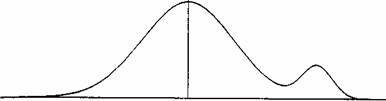
\includegraphics[scale=0.6]{figures/fig-7.jpg}

--- Вот высокие девушки. Проблема в этом прогибе. --- Он указывает на седловину между пиком и бугорком. Потом рисует новый пик, шире и выше, который бы их скрыл.

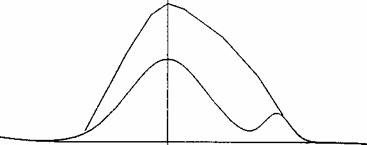
\includegraphics[scale=0.6]{figures/fig-8.jpg}

--- Этого можно добиться, подбрасывая в канал Руди сфабрикованные данные о несуществующих девушках выше среднего роста, но ниже тех, которые обслуживают <<Бомбы>>.

--- Однако теперь вы роете себе новую яму, --- говорит Чаттан. Он подался вперед на вертящемся стуле и, держа сигарету перед лицом, разглядывает Уотерхауза через неподвижное облако дыма.

Уотерхауз говорит:

--- Новая кривая выглядит чуть лучше, потому что я заполнил провал, но она еще не вполне колокол. Она не выгибается по краям, как положено. Доктор фон Хакльгебер это заметит. Он поймет, что кто то подбрасывает данные в канал. Чтобы этого избежать, я бы сфабриковал еще данные, добавив необычно большие и необычно малые величины.

--- Сочинили бы исключительно низких и исключительно высоких девушек, --- говорит Чаттан.

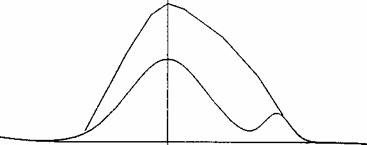
\includegraphics[scale=0.6]{figures/fig-8.jpg}

--- Да. Тогда кривая изогнется по краям, как положено.

Чаттан по прежнему смотрит на него выжидающе.

Уотерхауз говорит:

--- Так добавление небольшого количества данных, которые по отдельности казались бы аномальными, создает впечатление абсолютной нормальности.

--- Как я и сказал, --- говорит Чаттан. --- Сейчас, пока мы разговариваем, наш взвод в Северной Африке растягивает колокол. Придает ему абсолютно нормальный вид.


\chapter{МЯСО}


О'кей, рядовой первого класса Джеральд Готт из Чикаго, Иллинойс, за время своей пятнадцатилетней службы в рядах Вооруженных Сил США не хватал звания каждые день. Зато он классно вырезал отбивные. Он орудовал мясницким ножом ничуть не хуже, чем Бобби Шафто --- штыком, и кто скажет, что армейский мясник, экономно разделывая тушу и досконально соблюдая все санитарные предписания, спас меньше жизней, чем стальноокий боец? Война --- это не только убивать нипов, фрицев, даго. Война --- это еще и убивать скот. И есть его. Джеральд Готт, боец на передовой, содержал свою морозильную камеру в хирургической чистоте; только справедливо, что в ней он и встретил свою смерть.

Бобби Шафто сочиняет в голове это маленькое надгробное слово, дрожа от субарктической стужи в бывшей французской, а ныне американской морозильной камере, которая размерами и температурой легко могла бы потягаться с Гренландией. Кроме него, в камере --- бренные останки нескольких стад и одного мясника. За короткую службу Шафто перевидал немало похорон и всегда изумлялся искусству, с каким полковые капелланы возносят трогательные хвалы покойному. По слухам, когда вояки получают белобилетников, у которых на месте мозги, их учат печатать на машинке и сажают в кабинете день за днем строчить такое фуфло. Неплохая работенка.

Замершие туши длинными рядами висят на крюках. Бобби Шафто с каждым шагом все больше напрягается, готовясь к тому, что предстоит увидеть. В каком то смысле почти лучше, когда снаряд сносит приятелю голову вместе с нераскуренной сигаретой --- пока вот так собираешься с духом, недолго рехнуться.

Наконец Шафто огибает ряд и видит на полу человека в обнимку со свиной тушей, которую явно намеревался разделать за мгновение до смерти. Покойник тут уже двенадцать часов, и температура его тела --- минус двадцать градусов по Цельсию.

Бобби Шафто заставляет себя взглянуть на тело и набирает полную грудь холодного, пахнущего мясом воздуха. Складывает посиневшие руки в молитвенном и в то же время согревающем жесте. <<Господи! --- говорит он вслух. Эха нет --- туши поглощают звук. --- Прости этого морпеха за то, что он собирается сделать, и уж заодно обязательно прости его командиров, которых Ты в Своей безграничной мудрости соизволил над ним поставить, и прости их начальство за всю эту затею>>.

Шафто собирается продолжить, но решает, что грех тут не больше, чем закалывать нипов штыком. Ладно, к делу. Он подходит к сплетенным рядовому первого класса Джеральду Готту и Свинке --- Ледяной Щетинке, пытается их разделить, но безуспешно. Тогда он садится и начинает разглядывать мясника. Готт --- блондин. Глаза полузакрыты. Шафто светит в них фонариком и видит голубоватый отблеск. Готт --- не хилого сложения, фунтов на двести двадцать потянет, а то и на двести пятьдесят. Жизнь при армейской кухне не способствует похуданию, а также (к несчастью для Готта) поддержанию сердечно сосудистой системы в стабильно работающем состоянии.

Когда у Готта случился сердечный приступ, одежда на нем была сухая, поэтому, слава те господи, не прилипла к телу. Шафто в несколько движений срезает ее ножом V 44 <<Гун хо>>, заточенным, как бритва. Однако широкое девятисполовинойдюймовое лезвие V 44 не годится для ближнего боя, а именно для подмышек и паха, а Шафто строго приказано не поцарапать тело, поэтому он вынимает семисчетвертьюдюймовый обоюдоострый рейдерский стилет, как нарочно созданный для такого рода работы (хотя цельнометаллическая рукоятка через некоторое время начинает примерзать к потной ладони Шафто).

Лейтенант Этридж маячит сразу за дверью морозильной камеры. Шафто протискивается мимо него и направляется прямиком на улицу, не обращая внимания на несущееся вслед: <<Шафто? Ну как?>>

Останавливается, только выйдя из тени здания. Североафриканская жара омывает тело, как ванна с морфием. Он закрывает глаза и подставляет солнцу лицо, складывает ладони лодочкой. Тепло из горсти льется в руки, просачивается к локтям.

--- Ну как? --- снова спрашивает Этридж.

Шафто открывает глаза и смотрит по сторонам. Залив --- голубой полумесяц с бесчисленными песчаными косами, которые вьются одна вокруг другой, словно диаграмма танцевальных шагов. Одна утыкана гнилыми пеньками древних бастионов, рядом еще дымится полузатонувший французский линкор. Повсюду с невероятной скоростью разгружаются корабли операции <<Факел>>. Грузовые сетки взмывают над трюмами и шмякаются на пристань, как исполинские сопли. Грузчики таскают, грузовики возят, французские девушки курят американские сигареты, алжирцы предлагают сделки.

Между мясоразделочным цехом здесь, на горе, и кораблями раскинулся, насколько понимает Бобби, город Алжир. На его привередливый висконсинский взгляд город не столько выстроен, сколько разбросан по берегу приливом. Уйма площади отведена под защиту от солнца, поэтому у города наглухо задраенный вид --- много красной черепицы, украшенной зеленью и арабами. Несколько современных бетонных зданий вроде мясоразделочного цеха воздвигли французы в припадке сноса трущоб. Однако тут еще сносить и сносить. Кандидат номер один --- человеческий улей или муравейник слева от Шафто, касба\footnote{Касба (арабск. ) --- крепость.} или как там ее зовут. Может, это район, может, одно огромное несуразное здание. Арабы набились туда, как студенческая кодла в телефонную будку.

Шафто оборачивается и смотрит на морозильную камеру. Здесь на горе, она представляет собой идеальную цель для атак с воздуха, но всем глубоко насрать --- что за беда, если фрицы разбомбят гору мяса?

Лейтенант Этридж --- почти такой же обгоревший, как Шафто --- щурится.

--- Блондин, --- говорит Шафто.

--- Отлично.

--- Голубоглазый.

--- Еще лучше.

--- Муравьед. Не шампиньон.

--- А?

--- Не обрезан, сэр!

--- Замечательно! Как насчет остального?

--- Одна татуировка, сэр!

Шафто забавляет растущее волнение в голосе Этриджа.

--- Опишите татуировку, сержант!

--- Сэр! Распространенный армейский рисунок, сэр! Сердце, а в нем женское имя!

--- Какое имя, сержант? --- Этридж сейчас описается от волнения.

--- Сэр! Имя на татуировке --- Гризельда, сэр!

Лейтенант Этридж с шумом выпускает воздух. Женщины в покрывалах оборачиваются. В касбе какие то малохольные придурки высовываются из длинных тощих башен и начинают завывать не в лад.

Этридж, чтобы успокоиться, до белизны сжимает кулаки. Потом севшим от волнения голосом говорит:

--- Меньшая удача, чем эта, решала исход сражений!

--- Вы мне рассказываете?! --- отвечает Шафто. --- Когда я был на Гуадалканале, сэр, нас зажало в бухточке и...

--- Я не желаю слушать про ящерицу, сержант!

--- Сэр! Есть, сэр!


Однажды, еще в Окономовоке, Бобби Шафто пришлось вместе с братом заносить по лестнице матрас. Тогда он и научился с уважением относиться к тяжелым, но мягким предметам. Готт, упокой Господи его душу, тяжелый, как сволочь, и большая удача, что он насквозь промерз. Под средиземноморским солнцем он довольно скоро размякнет. И не только.

Все подчиненные Шафто находятся в зоне действий подразделения --- в пещере, пробитой в искусственном обрыве над доками. Такие пещеры тянутся на мили. Над ними --- бульвар. Однако все подходы к этой конкретной пещере замаскированы брезентом, чтобы никто, даже войска союзников, не видел, что там делают: выискивают веши, на которых написано 2701, замазывают единицу и набивают по трафарету двойку. Первую операцию выполняют рядовые с банками зеленой краски, вторую --- с черной и белой.

Шафто выбирает по человеку из каждой цветовой группы чтобы не стопорить работу. Солнце здесь зверское, однако в пещере, куда к тому же задувает с моря, жить можно. От теплых, свежепокрашенных поверхностей сильно воняет скипидаром. На Шафто этот запах действует умиротворяюще, потому что в бою ничего не красят, и в то же время отзывается в душе легким трепетом, потому что красят часто непосредственно перед боем.

Шафто собирается ознакомить трех избранных морпехов с заданием, но тут рядовой с черной краской на руках, Даньелс, смотрит через его плечо и ухмыляется.

--- Как по вашему, сержант, что лейтенант сейчас ищет? --- спрашивает он.

Шафто, рядовой Нейтан (зеленая краска) и рядовой Бранф (белая) разом оборачиваются и видят, что лейтенант Этридж отвлекся. Он снова роется в мусорных бачках.

Этридж выпрямляется и как можно укоризненнее демонстрирует стопку резных фанерок.

--- Сержант! Вы можете сказать, что это такое?

--- Сэр! Стандартные трафареты армейского образца, сэр!

--- Сержант! Сколько букв в алфавите?

--- Двадцать шесть, сэр! --- четко отвечает Шафто.

Рядовые Даньелс, Нейтан и Бранф переглядываются: сержант Шафто не лыком шит!

--- А сколько всего цифр?

--- Десять, сэр!

--- А из тридцати шести букв и цифр сколько не использовано в этих трафаретах?

--- Тридцать пять, сэр! Все за исключением цифры два, которая только и нужна для выполнения приказа, сэр!

--- Вы забыли вторую часть моего приказа, сэр!

--- Сэр! Так точно, сэр. --- Без толку отпираться. На самом деле офицеры даже любят, когда ты забываешь приказ: они чувствуют, что много умнее и толковее тебя. Ощущают свою нужность.

--- Второй частью моих приказов было: принять строжайшие меры к тому, чтобы не осталось никаких следов изменения!

--- Сэр! Так точно, сэр. Теперь вспомнил, сэр!

Лейтенант Этридж, который поначалу было раскипятился, теперь немного успокаивается. Подчиненные, которые знают его всего шесть часов, с одобрением отмечают про себя, что лейтенант --- человек отходчивый. Теперь он говорит спокойно и дружески, как свойский учитель старших классов. На нем армейские солнцезащитные очки, которые бойцы между собой называют <<Отпор насильнику>>. Они удерживаются на голове широкой черной резинкой. Лейтенант Этридж выглядит в них умственно отсталым.

--- Если вражеский шпион залезет в этот мусорный бачок, чем шпионы нередко занимаются, что он увидит?

--- Трафареты, сэр.

--- Если он сосчитает буквы и цифры, то заметит ли что нибудь необычное?

--- Сэр! Все они будут чистые, за исключением цифры два, которая отсутствует либо покрыта краской, сэр!

Лейтенант Этридж несколько минут молчит, чтобы подчиненные прониклись услышанным. На самом деле никто ни хера не понял. В воздухе сгущается гроза, но тут сержант Шафто поворачивается к рядовым.

--- Живо, ребята, замазать на хер все эти сраные трафареты! --- рявкает он.

Морпехи бросаются на мусорные бачки, словно на японские доты. Лейтенант Этридж, по всей видимости, удовлетворен. Бобби Шафто, набравший множество очков, ведет рядовых Даньелса, Нейтана и Бранфа наверх, к холодильнику, пока лейтенант Этридж не догадался, что он скомандовал наугад.

Все они успели побывать в смертельных боях, иначе не угодили бы в такую передрягу: посреди щедрого на опасности континента (Африка) в окружении врага (армии Соединенных Штатов Америки). Тем не менее, когда они заходят в морозильник и видят рядового первого класса Готта, все замолкают.

Рядовой Бранф складывает руки, украдкой трет их одна о другую.

--- Господи... --- начинает он.

--- Отставить, рядовой, --- говорит Шафто. --- Я уже.

--- О'кей, сержант.

--- Пилу принеси! --- говорит Шафто рядовому Нейтану.

Рядовые замирают.

--- Для гребаной свиньи! --- поясняет Шафто. Потом поворачивается к рядовому Даньелсу, который держит неприметный сверток, и говорит: --- Разворачивай!

В свертке (который выдал Этридж) оказывается черный гидрокостюм. Ничего армейского, какая то европейская модель. Шафто разворачивает его и осматривает по частям, пока рядовые Нейтан и Бранф расчленяют Ледяную Щетинку мощными движениями пилы.

Некоторое время работают молча, но тут вмешивается новый голос. <<Господи...>> --- начинает он. Все поднимают головы. Рядом с ними стоит человек, молитвенно сложив руки. Слова, сгущенные в сакраментальное и зримое облако, скрывают его лицо. Форму и звание не различить, потому что на плечах у него армейское одеяло. Он походил бы на пророка --- хоть сейчас на верблюда и в Святую Землю, --- если бы не чисто выбритый подбородок и очки <<Отпор насильнику>>.

--- Иди ты... --- говорит Шафто. --- Без тебя помолились.

--- Однако мы молимся о рядовом Готте или о себе? --- спрашивает незнакомец.

Трудный вопрос. Рядовые Нейтан и Бранф перестают пилить, наступает полная тишина. Шафто бросает гидрокостюм и выпрямляется. У человека в одеяле очень короткий седой ежик или просто изморозь осела на лысине. Льдистые глаза смотрят на Шафто через метровые стекла очков <<ОтНас>>, словно и впрямь ожидая ответа. Шафто делает шаг вперед и замечает на незнакомце пасторский воротничок.

--- Вот вы нам и объясните, преподобный, --- говорит Шафто.

Тут он узнает человека в одеяле и чуть не гаркает: <<Ты то какого хрена здесь?>>, но что то его удерживает. Капеллан делает движение глазами, такое быстрое, что замечает лишь Шафто, который стоит с ним практически нос к носу. Оно значит: <<Заткнись, Бобби, после поговорим>>.

--- Рядовой Готт сейчас с Богом или куда там люди отправляются после смерти, --- говорит Енох <<зови меня брат>> Роот.

--- Это еще как? Разумеется, он с Богом. Черт возьми! <<Куда там люди отправляются после смерти>>. Какой вы, на хер, капеллан?

--- Думаю, такой, какой нужен подразделению 2702, --- говорит капеллан. Лейтенант Енох Роот наконец отрывает глаза от Бобби Шафто и смотрит туда, где трудятся бойцы.

--- Чего, ребята, --- говорит он. --- Смотрю, сегодня на ужин свининка?

Рядовые нервно хихикают и снова берутся за пилу.

Как только удается освободить Готта от свиной туши, все четверо морпехов хватают его за руки --- за ноги. Готта волокут в разделочный цех, временно эвакуированный, чтобы его собратья по топору не разнесли слухов.

Поспешная эвакуация разделочного цеха после того, как одного из мясников нашли на полу мертвым, сама по себе может породить слухи. Легенда, наскоро сочиненная и запущенная лейтенантом Этриджем, такова: подразделение 2702 (вопреки очевидности) на самом деле элитная санчасть, а рядового Готта подкосила новая редкая форма североафриканского пищевого отравления. Может быть, ее даже нарочно оставили французы, немного обиженные на то, что потопили их линкор. Так или иначе, весь цех (гласит легенда) придется закрыть на день и вылизать дочиста. Тело Готта перед отправкой родным кремируют, чтобы опасная зараза не поразила Чикаго --- всемирную столицу скотобоен, --- где ее неисчислимые последствия способны повлиять на исход войны.

Для правдоподобия на полу установлен солдатский гроб. Шафто и его бойцы, не обращая на гроб внимания, натягивают на труп сначала жуткого вида плавки, потом --- отдельные части гидрокостюма.

--- Эй! --- говорит Этридж. --- Я думал, перчатки под конец.

--- Сэр, мы наденем их сначала, с вашего разрешения, сэр! --- говорит Бобби Шафто. --- Поскольку пальцы отмерзнут первыми, и тогда капец, сэр!

--- Хорошо, но прежде наденьте вот это, --- говорит Этридж и протягивает наручные часы. Шафто взвешивает их на руке и присвистывает: это швейцарский хронометр в массивном корпусе чистого урана, механизм на множество камней тикает, как сердце маленького зверька. Шафто покачивает их на браслете из ловко пригнанных металлических пластин. Такой штуковиной можно оглушить щуку.

--- Шикарно, --- говорит Шафто, --- только время не больно точно показывают.

--- Для того часового пояса, куда мы направляемся, --- говорит Этридж, --- точно.

Шафто, утершись, берется за работу. Тем временем лейтенанты Этридж и Роот вносят свою лепту в общее дело. Они несут куски Ледяной Щетинки на гигантские весы. Получается тридцать килограммов, хотя Шафто, привыкшему к фунтам, это ничего не говорит. Енох Роот обнаруживает похвальный аппетит к физическому труду (что молча отмечают про себя рядовые): он приволакивает и бросает на весы еще тушу. Вместе выходит семьдесят. Дальше они доводят вес до ста тридцати, таская окорока из холодильника. Енох Роот, который похоже, накоротке с этой чудною системой мер, посчитал и, дважды проверив, установил, что вес Джеральда Готта в килограммах --- сто тридцать.

Все мясо отправляется в гроб. Этридж захлопывает крышку вместе с несколькими мухами, которые пока не знают, на что себя обрекли. Роот с молотком в руках обходит гроб, заколачива здоровенные гвозди мощными, точными ударами Плотника из Назарета. Тем временем Этридж достает из портфеля свод инструкций. Шафто стоит близко и может прочесть большие печатные буквы на зеленой обложке.


ИНСТРУКЦИИ ПО ЗАПЕЧАТЫВАНИЮ ГРОБА

ЧАСТЬ III: ТРОПИЧЕСКИЙ КЛИМАТ

ТОМ II: ОПАСНАЯ ЭПИДЕМИОЛОГИЧЕСКАЯ ОБСТАНОВКА (БУБОННАЯ ЧУМА И Т.П.)


Два лейтенанта битый час выполняют инструкцию. Она не настолько сложна, однако Енох Роот все время находит синтаксические двусмысленности и начинает в них углубляться. Этридж сперва немного досадует, потом доходит до белого каления и, наконец, до крайнего прагматизма. Чтобы нейтрализовать капеллана, он изымает инструкцию и поручает Рооту по трафарету наносить на крышку фамилию <<Готт>> и лепить на нее красные наклейки с предупреждениями столь грозными, что от одних заголовков может хватить кондратий. Когда Роот заканчивает работу, открыть гроб имеет право только лично председатель Объединенного комитета начальников штабов генерал Джордж К. Маршалл, и то не раньше, чем получит разрешение главного военного врача и эвакуирует все живое в радиусе ста миль.

--- Как то капеллан смешно говорит, --- замечает на определенном этапе рядовой Нейтан, ошалело слушая дебаты Роота --- Этриджа.

--- Ага! --- восклицает рядовой Бранф, будто Нейтан проявил особую наблюдательность. --- Что это за акцент?

Все взгляды обращаются к Шафто. Тот делает вид, что прислушивается, потом объявляет:

--- Ну, ребята, я бы сказал, что предки Еноха Роота --- голландские и, может быть, немецкие миссионеры на островах Тихого океана и что женились они на австралийках. Более того, думаю, родился он на территории, которую контролируют британцы, паспорт у него английский, его мобилизовали в начале войны, и сейчас он входит в состав АНЗАК\footnote{Австралийского и Новозеландского экспедиционного корпуса.}.

--- Ух ты! --- восклицает рядовой Даньелс. --- Если все это окажется правдой, плачу пять баксов.

--- Идет, --- отвечает Шафто.

Этридж и Роот заканчивают с гробом. Примерно в то же время морпехи натягивают на покойника последнюю деталь гидрокостюма. Ушла чертова куча талька, но в конце концов справились. Тальк --- не американский; Этридж выдал им коробку какого то европейского. Над некоторыми буквами на этикетке --- две точки; Шафто знает, что это характерно для немецкого языка.

К воротам задом подъезжает грузовик. От него пахнет свежей краской (это грузовик подразделения 2702). В кузов загружают запечатанный гроб и одетого в резину мертвого мясника.

--- Я останусь и проверю мусорные бачки, --- говорит лейтенант Этридж. --- Встретимся на взлетном поле через час.

Шафто представляет себе час в раскаленном грузовике с таким грузом.

--- Обложить его льдом, сэр? --- спрашивает он.

Этридж задумывается: цыкает зубом, смотрит на часы, сопит, хмыкает. Однако, когда он вновь открывает рот, ответ звучит вполне определенно:

--- Нет. Для целей миссии существенно перевести его в размороженное состояние.

Рядовой первого класса Джеральд Готт и нагруженный мясом гроб занимают середину кузова. Морпехи сидят вдоль бортов, как почетный караул. Шафто смотрит через груду мертвечины на Еноха Роота, который старательно делает невозмутимый вид. Шафто понимает, что надо ждать, но утерпеть не может.

--- Что вы здесь делаете

? --- спрашивает он.

--- Подразделение перебрасывается, --- говорит преподобный, --- ближе к линии фронта.

--- Мы только что с корабля, --- отвечает Шафто. --- Разумеется, мы приближаемся к линии фронта. Удаляться можно было бы только вплавь.

--- Пока мы на колесах, --- спокойно говорит Роот, --- куда все, туда и я.

--- Я не про это, --- говорит Шафто. --- Я про то, зачем подразделению капеллан?

--- Вы не вчера в армии, --- говорит Рост. --- В каждой части должен быть капеллан.

--- Дурной знак.

--- Дурной знак иметь в части капеллана? Почему?

--- Значит, эти жопотрясы считают, что будет много похорон.

--- Вы придерживаетесь того мнения, что священник нужен только на похоронах? Занятно.

--- И на свадьбах с крестинами, --- говорит Шафто. Остальные морпехи давятся смехом.

--- Не смущает ли вас несколько первое задание подразделения 2702? --- спрашивает Енох Роот, выразительно глядя сперва на покойного Готта, потом на Шафто.

--- Смущает? Послушайте, преподобный, на Гуадалканале я делал такое, по сравнению с чем все вот это --- занятие для благовоспитанных школьниц, так их за ноги.

Остальные морпехи считают, что Шафто отбрил, так отбрил, однако Роот не унимается:

--- А вы знаете, зачем делали это на Гуадалканале?

--- Ясное дело! Чтобы остаться в живых.

--- А сейчас зачем?

--- Хер его знает.

--- Раздражает вас это немножко? Или вы просто тупой солдафон, которому все до лампочки?

--- Да, преподобный, тут вы меня поддели, --- говорит Шафто и, помолчав, добавляет: --- Признаюсь, малость любопытно.

--- Пригодился бы в подразделении 2702 человек, способный ответить <<зачем>>?

--- Наверное, --- нехотя соглашается Шафто. --- Просто дико как то, что у нас капеллан.

--- Почему дико?

--- Потому что это такое подразделение.

--- Какое? --- спрашивает Роот не без некоего садистского удовольствия.

--- Не положено говорить, --- отвечает Шафто. --- Да я и не знаю.

С горы вьются исполинские серпантины и, пройдя через ряд полосатых арок, спускаются к железнодорожным путям. <<Стоишь тут, на хер, как в лотке пинболла>>, --- говорит Б. Шафто, глядя вверх, туда, откуда они только что приехали, и воображая, что может скатиться из касбы. Они едут на юг вдоль железнодорожных путей и оказываются на территории отвалов, угольных куч, дымовых труб. Шафто --- бойскаут с Великих озер --- узнает все словно через какую то бесконечную межкультурную зубчатую передачу.  Грузовик останавливается перед <<Société Algérienne d'Éclairage et de Force>>\footnote{Алжирская компания по освещению и электроснабжению (АКОЭ) (фр.).} --- уродливым колоссом с двумя дымовыми трубами, перед которым навалена самая высокая угольная куча. Они у черта на куличках, но их явно ждут. Здесь --- как и повсюду, где бы ни появилось подразделение 2702, --- проявляется странный Эффект Раздувания Званий. Гроб заносят в здание АКОЭ два лейтенанта, капитан и майор под присмотром полковника!  Рядовых вообще не видать; Шафто, простой сержант, с тревогой гадает, какую работу найдут ему. Одновременно сказывается Эффект Отсутствия Проволочек --- там, где Шафто ожидает бумажной волокиты по меньшей мере на полчаса, выбегает офицер, машет руками, и гроб пропускают.

Араб с красной консервной банкой на голове тянет на себя стальную дверцу; оттуда вырываются языки пламени, он сбивает их черной кочергой. Офицеры направляют гроб в дверь и толкают вперед, словно досылая снаряд в ствол шестнадцатидюймового карабина. Араб с жестянкой на голове захлопывает дверцу (кисточка на жестянке бешено прыгает) и, еще не опустив щеколду, принимается завывать, как те придурки в касбе. Офицеры все очень довольны и пишут в книжечки свои имена.

После всех этих довольно странных событий грузовик отъезжает от <<Société Algérienne d'Éclairage et de Force>> и снова ползет по серпантину в Алжир. Подъем такой крутой, что его приходится одолевать на первой скорости. Торговцы с печками на колесах не только не отстают, но еще и успевают печь на ходу лепешки. Трехногие псы бегают и дерутся под коленвалом. Кроме того, подразделение 2702 одолевают местные в красных жестянках, которые рвутся играть на гитарах из канистр, продавцы апельсинов, заклинатели змей и голубоглазые малые в бурнусах, которые предлагают какие то бурые комки, без обертки и этикетки. Их, как градины, можно классифицировать по аналогии с фруктами или спортивным инвентарем. Обычно они размером от вишни до бейсбольного мяча. В какой то момент капеллан под влиянием порыва меняет плитку <<Херши>> на комок размером с бейсбольный мяч.

--- Это что, шоколад? --- спрашивает Бобби Шафто.

--- Был бы шоколад, --- отвечает Роот, --- этот тип не стал бы менять его на <<Херши>>.

Шафто пожимает плечами.

--- Может, это говенный шоколад.

--- Или говно! --- выпаливает рядовой Нейтан. Всем ужасно смешно.

--- Слышали про Марию Хуанну? --- спрашивает Роот.

Шафто --- образцовый боец и вожак --- перебарывает желание ответить: <<Слышал?! Да я ее греб!>>

--- Это то же самое, только в концентрированном виде, --- говорит Енох Роот.

--- А вы то откуда знаете, преподобный? --- спрашивает рядовой Даньелс.

Преподобный ничуть не смущен.

--- Я здесь насчет Бога, да? Мне положено знать религиозную сторону?

--- Так точно, сэр!

--- Так вот, была некогда такая мусульманская группа --- гашишины, они ели эту штуку и шли убивать. И так в этом преуспели, что даже прославились, а их название в несколько измененном виде --- асассины --- вошло во все европейские языки в значении <<убийцы>>.

Наступает уважительное молчание. Потом сержант Шафто говорит:

--- Так хули мы ждем?

Они съедают по кусочку; Шафто как старший среди рядового и сержантского состава --- больше всех. Ничего не происходит.

--- Если мне и хочется кого убить, так только типа, который толкнул нам это говно, --- говорит он.


Лётное поле, в одиннадцати милях от города, работает более чем с проектной нагрузкой. Вокруг растут маслины и виноград, но дальше --- горы, а за ними --- песчаное пространство, равное по площади Соединенным Штатам Америки, причем сдается, что весь этот песок в воздухе и летит к аэродрому. Бесчисленные самолеты, по большей части <<дакоты>>, они же <<дугласы>>, вздымают огромные тучи пыли, которая оседает на языке и забивает ноздри. До Шафто не сразу доходит, что сухость в глазах и во рту лишь отчасти вызвана пылью. Слюна густеет, как замазка.

Подразделение настолько секретное, что на аэродроме никто даже не знает о его существовании. Здесь полно британцев. В пустыне британцы носят шорты, поэтому Шафто хочется потянуть их за нос. Он перебарывает это желание. Однако его явная враждебность к людям в шортах, равно как и просьбы указать дорогу к подразделению, настолько секретному, что его нельзя даже назвать, ведут к непониманию, недоверию и вообще подрывают дух англо американского добросоюзничества.

Впрочем, тут сержант Шафто соображает, что все, связанное с подразделением, должно быть где нибудь в стороне, под черным брезентом. Как и в других армейских частях, в подразделении 2702 что то в недостатке, что то в избытке. По всей видимости, в их распоряжение попала примерно половина брезента, изготовленного за прошлый год в Соединенных Штатах. Когда Шафто упоминает этот факт и начинает развивать свою мысль, на лицах у рядовых появляется странное выражение. Наконец Енох Роот говорит: <<Сперва исполинская ящерица, теперь черный брезент. Некоторым может показаться, что вы малость тронутый>>.

--- Сейчас я вам расскажу про тронутых, --- говорит Шафто и рассказывает, не забывая упомянуть лейтенанта Этриджа с его мусорными бачками. К концу рассказа все подразделение уже собралось по дальнюю сторону растянутого брезента. Ребята напряжены, за исключением новобранца, который, как одобрительно замечает Шафто, начинает понемногу отходить. Лежа на дне грузовика в черном гидрокостюме, он скорее переваливается, чем подпрыгивает на ухабах.

Тем не менее он еще не вполне отмяк, так что его несложно вытащить и загрузить в <<Дуглас>> --- небольшой самолет, переделанный для военных целей и (на скептический взгляд Шафто) утративший летные качества за счет двух огромных грузовых люков, разрезающих корпус почти пополам. Этот конкретный самолет столько летал над чертовой пустыней, что с винтов, капота и передней части крыльев песком содрало всю краску; отполированный металл блестит, словно приглашение для всех пилотов люфтваффе на три мили вокруг. Хуже того, из обшивки фюзеляжа, главным образом вокруг кабины пилота, торчат антенны. И не какие нибудь штыревые, а здоровенные решетки для барбекю. <<Эх, сюда бы ножовку>>, --- думает Шафто. Антенны смутно похожи на те, которые он таскал по лестнице со станции <<Альфа>> в Шанхае. Впрочем, все воспоминания перемешались. Когда он пытается их восстановить, то видит одно: каменная лестница в Маниле, окровавленный Христос спускается по ступенькам, таща на спине двухполосный коротковолновый диполь. Понятно, что быть этого не могло.

Хотя они на оживленном аэродроме, Этридж отказывается продолжать операцию, пока в небе хоть один самолет. Наконец он командует: <<Все, ПОШЛИ!>> Морпехи в грузовике приподнимают тело. Тут Этридж кричит: <<Нет, ПОГОДИТЕ!>>, и тело шмякают на пол. На пятый раз это уже не смешно. Наконец Джеральда Готта накрывают черным брезентом и заносят в самолет. Через несколько минут они в воздухе. Подразделение 2702 направляется на встречу с Роммелем.


\chapter{ЦИКЛЫ}


Начало ноября 1942-го, и хренова туча всего происходит повсюду, одновременно. Сам Зевс бы не разобрался, даже если бы мобилизовал кариатид --- сказал бы, забудьте, что мы вам говорили, просто бросайте свой груз. Под грохот рушащихся храмов он отправил бы их (вместе с теми наядами и дриадами, которых удалось наскрести) на краткосрочные курсы и, облачив в ладные бесполые формы СУАОВ --- Службы управления архивами олимпийского всевидения, --- засадил бы заполнять перфокарты три на пять дюймов. Пусть бы даже все кариатиды со своим хваленым терпением сутки напролет, напялив зеленые козырьки, простаивали перед машинами Холлерита и перфосчитывателями ЭТК --- все равно Зевс не сумел бы охватить ситуацию. Он бы впал в ступор и не знал, кого из смертных поражать молниями и к кому из связисточек или солдатиков бить клинья.

Лоуренс Притчард Уотерхауз сам теперь олимпиец не хуже других. У Франклина Делано Рузвельта, Уинстона Черчилля и еще нескольких человек в списке <<Ультра Мега>> тот же уровень допуска, но у них другие дела и заботы. Они не могут бродить по всемирной столице информационных потоков, заглядывать через плечо переводчикам и читать свежие расшифровки, когда те --- щелк щелк щелк --- выползают из ТАЙПЕКСов. Они не могут бегать от здания к зданию, собирая воедино сюжетные нити мирового повествования, пока девушки в одиннадцатом корпусе переключают провода из гнезда в гнездо, сплетая сеть, в которую послания Гитлера попадают, едва выйдя в эфир.

Вот, например, что знает Уотерхауз: битва под Эль Аламейном выиграна, Монтгомери стремительно гонит Роммеля на запад, через Киренаику, к далекому оплоту Оси в Тунисе. Однако все не настолько в ажуре, как может показаться. Если бы Монти оценил важность информации, поступающей по каналам <<Ультра>>, он бы действовал решительнее, окружал и брал в плен изолированные подразделения итальянцев и немцев. Однако он этого не делает, и Роммель отступает организованно, готовясь дать новое сражение, а в Блетчли парке кроют Монти последними словами за нежелание воспользоваться бесценными, однако недолговечными сокровищами разведданных.

А сейчас в Северо Западную Африку перебросили чертову уйму народа. Это называется операция <<Факел>>, ее цель --- зажать Роммеля между молотом (английскими войсками) и наковальней (американскими войсками). Или, если Монти не поторопится, наоборот. Операция кажется блестяще организованной, но это не так: Америка впервые наносит серьезный удар через Атлантику, поэтому на корабли загрузили абсолютно всех. Сотрудники радиоразведки, строя из себя десантников, театрально бежали к берегу по пояс в воде. Также в высадке участвовал американский контингент подразделения 2702 --- аварийная команда, составленная из отборных морских пехотинцев, прошедших огонь, воду и медные трубы.

Часть из них получила свой боевой опыт на Гуадалканале --- никому прежде не нужном островке в юго западной части Тихого океана, где Японская империя и Соединенные Штаты Америки спорят --- посредством оружия --- за право построить военную авиабазу. Судя по первым сообщениями, японская армия за время пребывания в Восточной Азии несколько утратила форму. Оказывается, изнасиловать все женское население Нанкина или перебить штыками беззащитных филиппинских крестьян еще не значит набраться боевого опыта. Японская армия по прежнему пытается придумать, как бы, скажем, убить сто американских морских пехотинцев, не потеряв на этом пятьсот своих.

Другое дело --- японские ВМС. Они свое дело знают. У них есть Ямамото. Их торпеды действительно взрываются, попав в цель, в отличие от американских, которые, слегка поцарапав краску японских кораблей, виновато идут ко дну. Ямамото только что сделал очередную попытку уничтожить американский флот у островов Санта Крус, потопил <<Хорнет>>, проделал аккуратную дыру в <<Энтерпрайзе>>. Однако он потерял треть своих самолетов. Наблюдая, как японцы несут потери, Уотерхауз гадает, сообразил ли кто нибудь в Токио взять счеты и прикинуть кое какие цифры.

Союзники тоже считают и напуганы до потери пульса. В Атлантике сейчас сто немецких подлодок, они ведут действия главным образом из Лорьяна и Бордо. То, что там происходит, уже не битва, а вакханалия убийства в масштабах <<Лузитании>>\footnote{Английский пассажирский лайнер <<Лузитания>> был торпедирован немецкой подводной лодкой 7 мая 1915 года. Из 1959 человек пассажиров и команды 1198 утонули.}. За последний месяц немцы потопили кораблей в общей сложности на миллион тонн. Попробуй осознай!.. Положим, тонна --- примерно автомобиль. Уотерхауз пытается представить себе, что Америка и Канада сбросили в середину Атлантики миллион автомобилей. Бултых!

Проблема в Акуле.

Немцы зовут ее <<Тритон>>. Это новая шифросистема, используемая исключительно на флоте. <<Энигма>>, но не обычная, трехдисковая. Ту поляки научились взламывать два года назад, а в Блетчли парке процесс поставили на поток. Однако меньше года назад у южного берега Исландии села на мель немецкая подводная лодка. Сотрудники Блетчли парка хорошенько ее прочесали и нашли <<Энигму>> с выемками для четырех, а не для трех дисков!

Когда первого февраля заработали четырехдисковые <<Энигмы>>, вся Атлантика почернела. С тех самых пор Алан и другие не покладая рук бились над этой задачей. Загвоздка была в том, что они не знали, как подсоединен четвертый диск.

По счастью, несколько дней назад захватили еще одну немецкую подводную лодку, в восточной части Средиземного моря. Полковник Чаттан, оказавшийся поблизости, и еще несколько сотрудников Блетчли рванули туда сломя голову. Они нашли четырехдисковую <<Энигму>>, а это хоть не сам код, но по крайней мере ключ к его взлому.

Гитлер, видать, совершенно в себе уверен --- собрался отдохнуть в Альпах. Что не помешало ему прибрать к рукам последние остатки Франции --- похоже, операция <<Факел>> задела его за живое, и он окончательно оккупировал вишистскую Францию. Одновременно он отправил еще десять тысяч солдат и соответствующее количество припасов через Средиземное море в Тунис. Уотерхауз воображает, что сейчас можно добраться от Сицилии до Африки, просто прыгая с одного немецкого транспорта на другой.

Разумеется, будь это так, его работа была бы куда легче. Союзники топили бы суда сколько душе угодно, и ни один голубоглазый тевтон на фронте информационной войны не повел бы арийской бровью. Однако на самом деле судов мало и расположены они редко. Насколько именно мало и редко --- это параметры уравнений, которые они с Аланом Матисоном Тьюрингом всю ночь пишут на доске.

Часов через десять --- двенадцать этого занятия, когда наконец снова встает солнце, остается разве что сесть на велосипеды и прокатиться с ветерком.


Они въезжают на холм, и перед ними открывается лес, расцвеченный всеми цветами пламени. Полусферические кроны кленов словно вспучиваются в огне, добавляя впечатлению реализма. У Лоуренса возникает нелепое желание выпустить руль и зажать уши! Однако воздух под деревьями приятно прохладен, синее небо не пятнают столбы черного дыма, спокойствие и тишина леса самым разительным образом отличаются от того, что вспомнилось Лоуренсу.

--- Кудах тах тах! --- Алан Тьюринг изображает квохтание рассерженной курицы. Странные звуки кажутся еще чуднее из за того, что он в противогазе, который, впрочем, почти сразу сдвигает на лоб. --- Как же они любят себя слушать! --- (Речь об Уинстоне Черчилле и Франклине Рузвельте.) --- Да и друг друга тоже, до определенного момента. Однако голос по сравнению с печатным текстом --- жутко избыточный канал информации. Если взять текст и пропустить его через <<Энигму>> --- которая, в сущности, довольна проста, --- то привычные закономерности вроде преобладания буквы <<Е>> практически исчезают. --- Тут он снова натягивает противогаз, чтобы подчеркнуть следующее утверждение. --- А вот голос можно искажать самым чудовищным образом, и он все равно будет понятен слушателю.

Тут на Алана нападает приступ чихания, да такой, что чуть не лопаются защитного цвета ремешки на затылке.

--- Наше ухо привыкло отыскивать знакомые сочетания, --- предполагает Лоуренс. Он без противогаза, потому что (а) немцы не проводят здесь газовую атаку, (б) в отличие от Алана он не страдает сенной лихорадкой.

--- Прости. --- Алан резко тормозит и спрыгивает с велосипеда. Он отрывает заднее колесо от дороги, раскручивает его свободной рукой и быстрым движением дергает цепь. Потом внимательно созерцает механизм, прерываясь только для того, чтобы несколько раз чихнуть.

В цепи у велосипеда Тьюринга дефектное звено. В заднем колесе погнута одна спица. Когда звено задевает спицу, цепь сваливается и падает на дорогу. Это происходит не при каждом обороте колеса --- иначе велосипед проще было бы выкинуть. Это происходит при определенном взаимном расположении цепи и колеса.

Исходя из разумного предположения, что доктор Тьюринг находится в хорошей спортивной форме и развивает скорость примерно 25 км/час, а радиус колеса --- примерно треть метра, если бы дефектное звено задевало гнутую спицу при каждом обороте колеса, то цепь сваливалась бы каждую третью долю секунды.

На самом деле цепь не сваливается, пока гнутая спица не заденет дефектное звено. Теперь допустим, что вы описываете положение заднего колеса традиционной буквой Q. Ради простоты договоримся: если колесо начинает вращаться из положения, в котором гнутая спица может задеть дефектное звено (разумеется, только если дефектное звено находится там, где его можно задеть), то Q = 0. Если в качестве единицы измерения используются градусы, то за один поворот колеса Q принимает все значения вплоть до 359, прежде чем вернуться к нулю, когда гнутая спица вновь может сбросить цепь. Теперь предположим, что положение цепи вы описываете переменной С по очень простому принципу: нумеруя все звенья цепи. Дефектному звену ставится в соответствие число 0, следующему 1 и так далее до l-1, где l --- общее число звеньев в цепи. Опять таки ради простоты примем, что в положении, в котором дефектное звено может задеть гнутую спицу (при условии, что спица --- там, где ее можно задеть), С = 0.

Чтобы вычислить, когда с велосипеда доктора Тьюринга свалится цепь, все, что нам надо знать про велосипед, --- это значения Q и С . Эти два числа определяют состояние велосипеда. У велосипеда столько возможных состояний, сколько существует возможных значений (Q, С), но только в одном из этих состояний, а именно (0, 0), цепь свалится на дорогу.

Предположим, мы начинаем с этого состояния, т. е. (Q = 0, С = 0), но цепь не свалилась, потому что доктор Тьюринг (прекрасно зная состояние своего велосипеда в каждый конкретный момент времени) остановился посреди дороги и едва избежал столкновения со своим другом и коллегой Лоуренсом Притчардом Уотерхаузом, поскольку противогаз блокирует его периферическое зрение. Доктор Тьюринг немного прокрутил цепь вперед, одновременно оттягивая ее вбок, чтобы не задела за гнутую спицу. Теперь он снова садится на велосипед и начинает крутить педали. Окружность его колеса примерно два метра, значит, когда он проехал два метра по дороге, колесо совершило полный оборот и вернулось в состояние Q = 0, в котором, как мы помним, гнутая спица может задеть дефектное звено.

Что с цепью? Ее положение, определяемое как С, начинается с 0, достигает единицы, когда в фатальную позицию перемещается следующее звено, потом двойки и так далее. Цепь движется синхронно с зубцами звездочки в центре заднего колеса. У звездочки п зубцов, так что после второго полного оборота заднего колеса Q снова = 0, но С теперь = 2n. В следующий раз С = 3п и так далее. Однако не забывайте, что цепь --- не бесконечная прямая линия, а замкнутая петля, имеющая всего l позиций; при С = l, она возвращается к началу цикла, и С снова принимает нулевое значение. Так что при вычислении С следует прибегнуть к арифметике остатков: то есть если в цепи сто звеньев (l = 100), а общее число перемещенных звеньев --- 135, то значение С не 135, а 35. Как только вы получаете число, больше или равное l, вы просто последовательно вычитаете l, пока результат не станет меньше l. Математики обозначают эту операцию mod l. Так что последовательные значения С, всякий раз как заднее колесо возвращается в положение Q = 0, равны:

$$
C_i = n mod l, 2n mod l, 3n mod l, ..., in mod l
$$

где $i = (1, 2, 3, ... 8 \infty),$ меньше или больше в зависимости от того, насколько близкое к бесконечности время Тьюринг намерен ехать на велосипеде. Через некоторое время Уотерхаузу начинает казаться, что они и впрямь едут бесконечно.

Цепь сваливается, когда велосипед достигает состояния (Q = 0, C = 0). В свете вышесказанного это происходит, когда l (которое просто означает число оборотов, совершенных задним колесом) достигает некоего гипотетического значения, при котором in mod l = 0, или, говоря по человечески, когда некое число, кратное п (такое, как, например, 2n, 3n, 395n или 109 948 368 443n ), оказывается в то же время кратным l. Вообще то это может быть любое из так называемых общих кратных, но с практической точки зрения важно только первое --- наименьшее общее кратное, или НОК, поскольку именно оно будет достигнуто первым и вызовет падение цепи.

Если, скажем, у звездочки двадцать зубцов (n = 20), а в цепи сто звеньев (l = 100), то после первого поворота колеса мы имеем С = 20, после двух поворотов С = 40, потом 60, 80 и 100. Однако поскольку мы ищем остаток от деления на 100, значение надо изменить на ноль. Таким образом, после пяти оборотов колеса мы достигли состояния (Q = 0, С = 0) и цепь Тьюринга сваливается. За пять оборотов колеса он проезжает всего десять метров, поэтому при таких значениях l и n велосипед практически бесполезен. Разумеется, все это верно лишь в том случае, если Тьюринг такой дурак, чтобы начать движение из состояния спадения цепи. Если же он начинает крутить педали, когда велосипед находится в состоянии (Q = 0, С = 1), то С принимает значения 21, 41, 61, 81, 1, 21, ... и так до бесконечности, и цепь не свалится никогда. Однако это вырожденное состояние, где <<вырожденное>> для математика означает <<невыносимо скучное>>. В теории, если Тьюринг будет всякий раз выставлять нужное состояние, прежде чем бросить велосипед на улице, никто не сможет его украсть --- цепь свалится через первые же десять метров.

Если же в цепи Тьюринга сто одно звено (l = 101), то после пяти оборотов мы имеем С = 100, а после шести С = 19, тогда


С = 39, 59, 79, 99, 18, 38, 58, 78, 98, 17, 37, 57, 77, 97, 16, 36, 56, 76, 96, 15, 35, 55, 75, 95, 14, 34, 54, 74, 94, 13, 33, 53, 73, 93, 12, 32, 52, 72, 92, 11, 31, 51, 71, 91, 10, 30, 50, 70, 90, 9, 29, 49, 69, 89, 8, 28, 48, 68, 88, 7, 27, 47, 67, 87, 6, 26, 46, 66, 86, 5, 25, 45, 65, 85, 4, 24, 44, 64, 84, 3, 23, 43, 63, 83, 2, 22, 42, 62, 82, 1, 21, 41, 61, 81, 0.


Так что состояние (Q = 0, С = 0) не будет достигнуто и цепь не свалится, пока колесо не совершит сто один оборот. За сто один оборот велосипед Тьюринга успевает проехать по дороге пятую часть километра, что совсем не так плохо. Значит, велосипед работающий. Однако в отличие от вырожденного случая его нельзя привести в такое состояние, чтобы цепь не спадала совсем. Это легко доказать, просмотрев приведенный список значений С и убедившись, что все возможные значения --- все числа от одного до ста --- в нем присутствуют. Это означает, что с какого бы значения С Тьюринг ни начал крутить педали, рано или поздно он придет к фатальному С = 0 и цепь свалится.

Разница между вырожденным и невырожденным случаем заключена в свойствах использованных чисел. Комбинация (п = 20, l = 101) принципиально отличается от комбинации (п = 20, l = 100). Главная разница в том, что 20 и 101 --- <<взаимно простые>>, т. е. у них нет общих делителей. Это означает, что их наименьшее общее кратное, их НОК --- большое число и равняется собственно l x n, т. е. 20 x 101 = 2020. А вот НОК ста и двадцати --- всего 100. У велосипеда с l = 101 длинный период --- он проходит через множество различных состояний, прежде чем вернуться к исходному, а у велосипеда с l = 100 --- короткий, всего из нескольких состояний. Предположим, что велосипед Тьюринга --- шифромашина, основанная на алфавитной замене, т. е. заменяет каждую из двадцати шести букв английского алфавита какой то другой буквой. А открытого текста может стать Т шифртекста, В --- F, С --- М и так дальше до Z. Сам по себе такой шифр до смешного прост, взломать его --- детская забава. Однако предположим, что схема замены меняется от буквы к букве. Первая буква открытого текста шифруется с помощью одного алфавита замены, вторая --- с помощью другого, третья --- с помощью третьего и так далее. Это называется полиалфавитный шифр.

Предположим, что велосипед Тьюринга генерирует свой алфавит для каждого из состояний. Тогда состоянию (Q = 0, С = 0) будет соответствовать, например, такой алфавит замены:


A B C D E F G H I J K L M N O P Q R S T U V W X Y Z

Q G U W В I Y T F K V N D O H E P X L Z R C A S J M


а состоянию (Q = 180, С = 15) --- такой:


A B C D E F G H I J K L M N O P Q R S T U V W X Y Z

B O R I X V G Y P F J M T C Q N H A Z U K L D S E W


Никакие две буквы не будут зашифрованы одним и тем же алфавитом замены, пока велосипед не вернется в исходное состояние (Q = 0, С = 0) и цикл не пойдет с начала. То есть это периодическая полиалфавитная система. Теперь, если период у машины короткий, она часто повторяет саму себя и в качестве шифровальной системы тоже годится исключительно для детской забавы. Чем длиннее период (чем больше взаимно простых чисел в него встроено), тем реже используется один и тот же алфавит замены и тем выше устойчивость шифра.

Трехдисковая <<Энигма>> --- система именно такого типа (то есть периодическая полиалфавитная). Ее барабаны подобно приводу в велосипеде Тьюринга заключают в себе циклы в циклах. Ее период равен 17 576, то есть алфавит замены, которым зашифрована первая буква сообщения, не повторится до 17 577 й буквы. Однако в <<Акуле>> немцы добавили четвертый барабан, увеличив период до 456 976. В начале каждого сообщения диски ставятся в различные, случайным образом выбранные исходные положения. Поскольку ни в одном немецком сообщении нет 450 000 знаков, <<Энигма>> никогда не повторяет один и тот же алфавит замены в пределах отдельного сообщения. Вот почему немцы считают ее неуязвимой.

Над головами пролетает звено транспортных самолетов, направляясь, по всей видимости, к аэропорту в Бедфорде. Самолеты издают странно музыкальный диатонический гул, словно волынки, играющие две мелодии разом. Это напоминает Лоуренсу об еще одном феномене, связанном с велосипедным колесом и шифрмашиной <<Энигма>>.

--- Ты знаешь, почему самолеты так гудят? --- спрашивает он.

--- Нет, если задуматься. --- Тьюринг снова сдвигает противогаз на лоб. Челюсть у него немного отвисла, глаза смотрят в разные стороны. Уотерхауз его зацепил.

--- Я заметил в Перл Харборе. У самолета --- звездообразный двигатель, --- говорит Лоуренс. --- Соответственно, в нем должно быть нечетное число цилиндров.

--- Как одно из другого следует?

--- Если число будет четным, цилиндры окажутся один напротив другого, развернутые на сто восемьдесят градусов, а это не работает механически.

--- Почему?

--- Не помню. Не работает, и все.

Алан поднимает брови. Он явно не убежден.

--- Это как то связано с кривошипами, --- защищается Уотерхауз.

--- Не уверен, что соглашусь.

--- Просто допусти. Считай это граничным условием, --- говорит Уотерхауз. Однако Алан уже ушел в свои мысли --- наверное, изобретает звездообразный двигатель с четным числом цилиндров.

--- В любом случае, если посмотришь, у них у всех цилиндров нечетное число, --- продолжает Лоуренс. --- Поэтому шум выхлопа накладывается на гудение винта и получается двухтоновой звук.

Алан снова садится на велосипед. Некоторое время они едут молча. Собственно, они и до этого не столько разговаривали, сколько подкидывали друг другу идеи и давали время подумать. Это очень производительный способ общения; он устраняет значительную часть избыточности, на которую жаловался Алан в случае Рузвельта и Черчилля.

Уотерхауз думает о вложенных циклах. Он уже решил, что человеческое общество действует по этому самому принципу\footnote{У него нет никаких определенных фактов на этот счет, просто идейка кажется занятной.}, и теперь пытается понять, похоже оно на велосипед Тьюринга (некоторое время работает безотказно, потом внезапно цепь сваливается, отсюда --- мировая война), как <<Энигма>> (долго непонятно скрипит, потом вращающиеся диски выстраиваются, как в игровом автомате, и наступает всеобщее счастье, или, если предпочитаете, Апокалипсис), или просто как самолетный мотор (крутится себе и крутится, ничего особенно не происходит, кроме шума).

--- Смотри, сзади! Вон там! --- Алан резко тормозит. Это просто шутка, чтобы Лоуренсу пришлось сделать крутой поворот на узкой дороге.

Они прислоняют велосипеды к дереву и снимают с багажников оборудование: сухие батареи, макетные платы, палки, саперный инструмент, мотки провода.

--- Я скоро в Америку, работать над проблемой шифрования голоса в лабораториях компании <<Белл>>, --- говорит Алан.

Лоуренс невесело смеется.

--- Мы с тобой как те корабли у Лонгфелло, которые встретились в ночи, помигали сигнальными огнями и снова разошлись.

--- Мы пассажиры на этих кораблях, --- поправляет Алан. --- Это не случайность. Ты здесь именно потому, что я уезжаю. До сих пор всю работу подразделения 2701 тянул я.

--- Теперь это подразделение 2702, --- говорит Лоуренс.

Алан расстроен.

--- Заметил, значит.

--- Очень неосторожно с твоей стороны, Алан.

--- Наоборот! --- говорит Алан. --- Что подумает Руди, если заметит, что во всей армии союзников нет ни одного подразделения, номер которого был бы произведением двух простых чисел?

--- Ну, это зависит от того, насколько часто такие числа встречаются и сколько других чисел не использовано, --- говорит Лоуренс и начинает решать первую часть задачи. --- Опять риманова дзета функция. Везде она вылезает.

--- Вот это по мне! --- говорит Алан. --- Разумный, деловой подход. Не то что у них.

--- У кого?

--- Вот здесь. --- Алан останавливается и смотрит на деревья, которые, на взгляд Уотерхауза, ничем не отличаются от соседних. --- Вроде они. --- Он садится на упавший ствол и начинает доставать из рюкзака оборудование. Лоуренс садится рядом и тоже развязывает рюкзак. Он не знает, как работает устройство --- это изобретение Алана, --- и исполняет роль хирургической медсестры: по мере надобности подает инструмент и материалы. Доктор говорит без умолку, поэтому не просит подать нужную вещь, а смотрит на нее пристально и хмурится.

--- У кого по твоему? У придурков, которые используют информацию, полученную из Блетчли парка.

--- Алан!

--- Не придурки, скажешь? Возьми Мидуэй! Идеальный пример.

--- Ну, я был рад, когда мы выиграли сражение, --- осторожно замечает Лоуренс.

--- А тебе не показалось немного странным, немного удивительным, немного явным, что после всех блестящих обманных маневров Ямамото этот ваш Нимиц в точности знал, где именно его искать? В одном определенном месте всего Тихого океана?

--- Ладно, --- говорит Лоуренс. --- Я возмутился, докладную написал. Наверное, из за нее сюда и попал.

--- Так вот, мы, англичане, ничуть не лучше.

--- Да?

--- Если бы ты узнал, что мы творим в Средиземном море, ты бы ужаснулся. Это скандал. Преступление.

--- Что мы там творим? --- спрашивает Лоуренс. --- Я говорю <<мы>>, а не <<вы>>, потому что теперь мы союзники.

--- Да, да, --- нетерпеливо отвечает Алан. --- Так утверждают. --- Он замирает, проводит пальцем вдоль цепей схемы, рассчитывая в уме индуктивности. --- Ну, мы топим конвои. Немецкие конвои. Топим направо и налево.

--- Конвои для Роммеля?

--- Да. Немцы грузят топливо, танки и боеприпасы в Неаполе и отправляют суда на юг. Мы их топим. Топим почти все, потому что взломали итальянский шифр C38m и знаем, когда они выходят из Неаполя. А последнее время мы топим вообще все суда с припасами, которые особенно нужны Роммелю, потому что взломали его шифр <<Зяблик>> и знаем, что он настойчивей всего требует.

Тьюринг щелкает на своем изобретении тумблером. Пыльный конус из черной бумаги, привязанный к плате бечевкой, противно верещит. Конус --- это репродуктор, надо думать, из радиоприемника. Алан берет ручку от метлы с длинной проволочной петлей на конце (вдоль палки к плате тянется провод) и проводит ею на уровне пояса, пока петля, как лассо, не повисает перед Лоуренсом. Репродуктор вопит.

--- Отлично. Реагирует на твою пряжку, --- говорит Алан.

Он ставит конструкцию на сухие листья, роется в нескольких карманах и, наконец, вытаскивает листок, на котором печатными буквами написано несколько строчек. Лоуренс узнал бы листок где угодно: это дешифровальная ведомость.

--- Что там у тебя, Алан?

--- Я записал подробные инструкции, положил в пузырек из под амфетамина и спрятал под мостом, --- говорит Алан. --- На прошлой неделе я забрал пузырек и расшифровал инструкции. --- Он машет листочком в воздухе.

--- Какой шифровальный системой ты пользовался?

--- Моей собственной. Хочешь, попытайся взломать.

--- А почему решил выкопать именно сейчас?

--- Это была предосторожность на случай немецкого вторжения, --- говорит Алан. --- Теперь, когда вы вступили в войну, нас точно не оккупируют.

--- И много ты зарыл?

--- Два серебряных слитка, Лоуренс, каждый на сумму примерно сто двадцать пять фунтов. Один должен быть совсем близко.

Алан встает, вынимает из кармана компас, поворачивается лицом к северу и расправляет плечи. Потом поворачивается на несколько градусов.

--- Не помню, учел ли я магнитное склонение, --- бормочет он. --- Точно. Ладно, все равно. Сто шагов на север. --- Алан углубляется в лес. За ним идет Лоуренс, которому поручено нести металлоискатель.

Доктор Тьюринг может ехать на велосипеде и, не прерывая разговора, считать обороты педалей. Точно так же он может считать шаги и разговаривать. Впрочем, не исключено, что он просто давно сбился со счета.

--- Если все, что ты говоришь, правда, --- произносит Лоуренс, --- то мы наверняка допрыгались. Руди должен был сообразить, что мы взломали их коды.

--- Существовала неофициальная система, которую можно считать предшественницей подразделения 2701, или 2702, или как там мы его называем, --- говорит Алан. --- Когда мы хотим потопить конвой, то посылаем самолет разведчик. Разумеется, наблюдение --- не настоящая его цель, мы и без того знаем, где конвой. Цель --- пролететь так близко, чтобы его заметили. Тогда с корабля отправляют радиограмму, что их засек самолет службы наблюдения. Когда мы после этого их топим, немцы не удивляются --- во всяком случае, не настолько удивляются, чтобы понять истинное положение дел.

Алан останавливается, сверяется с компасом, поворачивает на девяносто градусов и начинает идти на запад.

--- По моему, это мертвому припарки, --- говорит Лоуренс. --- Насколько вероятно, что союзный разведчик, посланный наугад, случайно заметит все до одного конвои?

--- Я уже подсчитал и готов поспорить на любой из моих серебряных слитков, что Руди подсчитал тоже, --- отвечает Тьюринг. --- Вероятность очень мала.

--- Значит, я прав, --- говорит Лоуренс, --- и, судя по всему, мы допрыгались.

--- Может быть, еще нет. Пока все на волоске. На прошлой неделе мы потопили конвой в тумане.

--- В тумане?

--- Туман висел весь день. Засечь конвой с воздуха было нельзя. Эти кретины все равно его потопили. У Кессльринга, ясное дело, закрались подозрения. Тогда мы сфабриковали сообщение (зашифрованное кодом, который, мы точно знаем, нацисты вскрыли) к вымышленному агенту в Неаполе, в котором благодарили за информацию о конвое. С тех самых пор гестапо прочесывает портовые районы Неаполя --- ищет нашего человечка.

--- Значит, пока пронесло.

--- Да. --- Алан резко останавливается, забирает у Лоуренса металлоискатель и начинает водить петлей по поляне. Петля постоянно задевает о ветки и гнется, так что ее приходится выпрямлять, но упорно молчит, если только Алан для проверки не подносит ее к пряжке у Лоуренса на ремне.

--- Дело страшно тонкое, --- задумчиво произносит Алан. --- Некоторые офицеры ПСС в Северной Африке...

--- ПСС?

--- Подразделений спецсвязи. Они передают данные <<Ультры>> в полевые штабы и следят, чтобы их там уничтожили. Так вот, некоторые из них, узнав из <<Ультры>>, что в обеденное время будет немецкий авианалет, пришли в столовую с касками. Когда авианалет произошел в указанное время, многих заинтересовало, как они догадались прихватить каски.

--- Безнадега какая то, --- вздыхает Лоуренс. --- Почему же немцы до сих пор не догадались?

--- Нас это удивляет, потому что мы знаем все и наши каналы связи свободны от шума, --- говорит Алан. --- У немцев каналов связи меньше, а шума в них больше. Если мы не будем постоянно делать явные глупости, скажем, топить конвои в тумане, они никогда не получат однозначного доказательства, что мы взломали <<Энигму>>.

--- Забавно, что ты помянул <<Энигму>>, --- говорит Лоуренс, --- потому что этот канал содержит огромное количество шума, из которого мы ухитряемся извлекать массу полезной информации.

--- Именно поэтому я и беспокоюсь.

--- Ладно, я, как могу, постараюсь одурачить Руди.

--- Ты то справишься. Я беспокоюсь из за тех, кто выполняет операцию на местах.

--- Полковник Чаттан представляется вполне надежным. --- Лоуренс понимает, что успокаивать Алана бесполезно. У него просто такое настроение. Раз в два или три года Уотерхауз проявляет светский такт, и сейчас как раз такой случай: он меняет тему. --- Значит, займешься секретной телефонией для Рузвельта и Черчилля?

--- В теории. Сомневаюсь, что из этого выйдет что нибудь практическое. В лабораториях <<Белл>> есть система, основанная на том, что форму сигнала разбивают на несколько диапазонов... --- И Алан углубляется в рассказ о телефонных компаниях. Он выдает развернутый доклад о теории информации в приложении к человеческому голосу, и о том, как это влияет на телефонию. Хорошо, что у Тьюринга такая большая тема для изложения: лес большой, и он явно не помнит, где зарыл серебро.

Необремененные слитками серебра, друзья едут назад в сумерках, которые в этих северных широтах наступают на удивление рано. Они по большей части молчат: Лоуренс переваривает то, что Алан наболтал про подразделение 2702, конвои, лаборатории <<Белл>> и избыточность голосового сигнала. Каждые несколько минут их обгоняет мотоцикл с шифровками в багажном контейнере.


\chapter{НА ВЫСОТЕ}


Все, что годится для переброски скота, Бобби Шафто в разное время испробовал на себе --- телячьи вагоны, открытые бортовые машины, форсированные марши по пересеченной местности. Теперь военные придумали этим радостям воздушный аналог --- Самолет с Тысячью Имен: <<Дуглас>>, DC 3, <<старый толстяк>>, С 47, <<номер три>>, <<дакота>>, <<дуг>>. Голые алюминиевые ребра фюзеляжа пытаются забить Бобби до смерти, но он пока отбивается. Главное, не заснуть.

Рядовых затолкали во второй самолет. В этом --- лейтенанты Этридж и Роот вместе с рядовым первого класса Готтом и сержантом Бобби Шафто. Лейтенант Этридж подгреб под себя все, что было в отсеке мягкого, устроил гнездышко в передней части самолета и пристегнулся. Некоторое время он делал вид, что читает документы. Потом стал смотреть в иллюминатор. Сейчас он уснул и храпит так, что, кроме шуток, заглушает моторы.

Енох Роот забился в дальнюю, узкую часть фюзеляжа и читает две книги разом. Шафто думает, что это очень типично: книги наверняка говорят совершенно разные вещи, и капеллану нравится их стравливать --- есть же любители играть в шахматы за обоих игроков сразу. Наверное, когда живешь на горе, а туземцы вокруг не знают ни одного из десятка языков, которыми ты владеешь, поневоле научишься спорить с самим собой.

В обоих бортах самолета --- ряды маленьких квадратных иллюминаторов. Шафто смотрит направо и видит горы, покрытые снегом. Он в панике: неужели они сбились с пути и летят над Альпами? Однако слева по прежнему Средиземное море. Постепенно его сменяет каменистая местность, заросшая чахлым кустарником, из которого торчат каменные столбы вроде <<Башни Дьявола>> в Вайоминге, потом остаются только камни и песок или песок без камней. Там и сям без всяких видимых причин песок морщится барханами. Черт возьми, они все еще в Африке!

Безобразие, почему не видно львов, жирафов и носорогов?.. Шафто идет высказать претензию пилотам. Может, удастся перекинуться с земляками в картишки. Или из переднего окна кабины видно что нибудь такое, о чем можно будет написать домой.

Полный облом. Ничего в переднее окно не видно. Во всей вселенной есть только море, небо, песок. Каждый морпех знает, какое скучное это море. Песок и небо --- немногим лучше. Впереди облачная гряда --- какой то там атмосферный фронт. И все.

Шафто успевает в общих чертах ознакомиться с планом полета, прежде чем карту убирают подальше от его глаз. Судя по всему, они летят над Тунисом. Бред какой то. Когда Шафто интересовался последний раз, Тунис был под немцами и даже оставался их главным оплотом в Северной Африке. Судя по плану, они намерены лететь над проливом между Бизертой и Сицилией, потом на восток, к Мальте.

Припасы и подкрепления доставляют Роммелю через этот самый пролив и выгружают в Бизерте или Тунисе. Отсюда Роммель может ударить на восток, по Египту, или на запад, по Марокко. Несколько недель назад восьмая британская армия задала ему жару под Эль Аламейном (это как раз в Египте), и с тех самых пор он отступает к Тунису. Недавно в Северной Африке высадились американцы, но пока ему здорово удается сражаться на два фронта, насколько Шафто угадывает промеж строк информационных радиосводок --- уж больно они становятся бодрыми, как только речь заходит о Роммеле.

Все это означает, что под ними, в Сахаре, развернуты и готовы к бою крупные силы. Может быть, прямо сейчас идет сражение. Однако Шафто ничего такого не видит, только за редким караваном стелется пыль, словно дым вдоль бикфордова шнура.

Поэтому Шафто беседует с пилотами, пока по их взглядам не замечает, что говорит уже очень долго. Видать, эти гашишины убивали свои жертвы, забалтывая их до смерти.

На картишки рассчитывать нечего. Пилоты молчат, как в рот воды набрали. Приходится ввалиться в кабину и чуть ли не схватиться за рычаги, чтобы вытянуть из них хоть слово. Говорят они как то странно. Только тут до Шафто доходит, что они не земляки, а друзья. Они --- англичане.

Прежде чем убраться в грузовой отсек, он успевает заметить еще одно: оба пилота вооружены до зубов, как будто рассчитывают уложить человек двадцать --- тридцать по пути от самолета в сортир и обратно. Шафто успел повидать таких психов, и ему это не нравится. Уж очень напоминает Гуадалканал.

Он находит место на дне грузового отсека рядом с рядовым первого класса Готтом и ложится. Крошечный револьвер на поясе мешает лежать на спине. Шафто перекладывает его в карман Теперь главное неудобство --- зачехленный рейдерский стилет упрятанный между лопаток. Хочется лечь на бок, но с одной стороны казенный полуавтоматический кольт, которому он не доверяет, с другой --- свой проверенный шестизарядник. Приходится разместить это все на полу, вместе с запасными обоймами, патронташами и разнообразными принадлежностями.

Кроме того, приходится отстегнуть от левой лодыжки нож <<Гун хо>>, незаменимый при расчистке джунглей, вскрытии кокосовых орехов и обезглавливании нипов, а от правой --- короткоствольный крупнокалиберный пистолет, который Шафто носит для равновесия. Остаются только гранаты в передних карманах, потому что на животе он лежать не собирается.

Они огибают мыс как раз вовремя, чтобы их не унесло приливом. Впереди илистое дно бухточки. С одной стороны ее ограничивает мыс, который они только что обогнули, с другой, в нескольких ярдах впереди --- следующий, до тошноты похожий, с третьей --- вертикальный обрыв. Даже если бы он не был покрыт непроходимыми джунглями, взобраться все равно бы не удалось из за крутизны. Морпехи заперты в бухте до следующего отлива.

У нипского пулеметчика вдоволь времени, чтобы перестрелять их всех.

Они сразу узнают звук очереди и падают в ил. Шафто быстро оглядывается. Те, что лежат на спине или на боку, вероятно, мертвы. Те, что на животе, --- вероятно, живы. Большая часть лежит на животе. Сержант явно мертв --- пулеметчик первым делом целил в него.

Пулемет у нипа --- или нипов --- один, но патронов хоть отбавляй. Их доставляет <<Токийский экспресс>>, который беспрепятственно курсирует проливом Слот. Пулеметчик не спеша прочесывает бухту, быстро переключая огонь на тех морпехов, которые пытаются шевельнуться.

Шафто вскакивает и бежит к обрыву.

Наконец он видит вспышки. Они показывают, куда направлено пулеметное дуло. Когда они удлиненные, то на кого то другого. Когда становятся короче, это значит, что ствол разворачивается к Бобби Шафто...

Черт, не рассчитал. В нижней правой части живота жуткая боль. Ил заглушает крики: каска и ранец рюкзак вдавливают его мордой в жидкую грязь.

Кажется, он теряет сознание. Но ненадолго. Пулемет по прежнему трещит, значит, кто то из ребят еще жив. Шафто с трудом поднимает голову, пересиливая вес каски, и видит между собой и пулеметом бревно --- отполированный волнами плавник, далеко выброшенный штормом.

Можно бежать к бревну --- или не бежать. Шафто решает бежать. Это всего несколько шагов. На полпути он понимает, что успеет. Приходит наконец второе дыхание --- он делает стремительный рывок и падает за бревном. Десяток пуль глухо шмякаются о древесину, на Шафто сыплются мокрые волокнистые щепки. Бревно гнилое.

Плохо, что Шафто не может посмотреть вперед или назад, не приподнявшись над бревном. Других морпехов не видно, не слышно криков. Он решает взглянуть, где там пулеметчик. За растительностью почти ничего не видно, но похоже, огневая точка где то в пещере, футах в двадцати над отмелью. Шафто не так далеко от обрыва --- расстояние преодолевается в одну перебежку. Однако лезть на обрыв --- верная смерть. Вряд ли пулемет можно наклонить настолько, чтобы стрелять вниз, но тебя закидают гранатами или расстреляют из винтовки, пока будешь карабкаться по камням.

Другими словами, время для винтовочного гранатомета. Шафто перекатывается на спину, вытаскивает из полотняной амуниции ребристую металлическую насадку, прилаживает ее к винтовочному стволу, пытается прикрутить... Пальцы проскальзывают на чертовой гайке. Тыловое умники! Не догадались поставить здесь гайку барашек ! Крути --- не крути, без толку. Все вокруг в крови, но боли нет. Шафто трет пальцами по песку, чтобы не скользили, закручивает проклятую гайку.

Из подсумка извлекается осколочная граната Марк II, она же <<ананас>>, за ней --- гранатометное приспособление M1 с боевым зарядом. Одно вставляется в другое, выдергивается чека, все вместе забивается в ствол винтовочного гранатомета. Наконец Шафто лезет в специально помеченный патронташ, роется в гнутых и сломанных сигаретах, находит холостой патрон, который и заряжает в <<спрингфилд>>.

Он ползет вдоль бревна, чтобы выстрелить с неожиданного места --- тогда, может быть, не срежут голову очередью. Наконец поднимает всю эту систему ниппель, упирает приклад в песок (при стрельбе в режиме гранатомета отдача такая, что запросто сломает ключицу), направляет ее на врага, жмет на курок. Гранатометное приспособление M1 с грохотом вылетает, оставляя позади целую скобяную лавку ненужных деталей, словно душа, покинувшая грешное тело. <<Ананас>> взмывает ввысь, без чеки и предохранителя, химический запал горит так, что вся эта штука светится изнутри. Шафто не промахнулся, граната летит в цель. Он уже готов поздравить себя, но тут граната отлетает назад, катится с обрыва и взрывает соседнее гнилое бревно. Нины предусмотрели такую возможность и натянули противогранатную сетку.

Шафто лежит на спине в мокрой грязи, снова и снова твердит слово <<бля>>. Все бревно содрогается, что то похожее на мох сфагнум сыплется на лицо. Пули постепенно вгрызаются в гнилушку. Бобби Шафто приносит молитву Всевышнему и готовится лечь грудью на амбразуру.

Одуряющий треск пулеметной очереди смолкает, слышатся крики. Голос вроде незнакомый. Шафто приподнимается на локте и понимает, что крики несутся со стороны пещеры.

Он смотрит в большие, небесно голубые глаза Еноха Роста.

Капеллан оставил свой уютный уголок в дальней части самолета и сидит на корточках перед иллюминатором, цепляясь за что попало. Бобби Шафто, который во сне перекатился на живот, смотрит в иллюминатор противоположного борта. Он должен видеть небо, но за иллюминатором стремительно проносится бархан. На Шафто накатывает тошнота. Даже мысли нет о том, чтобы сесть.

Яркие пятна света стремглав носятся по грузовому отсеку, как шаровые молнии, но --- и поначалу это совсем не очевидно --- они бегают по стенам, как луч от фонарика. Шафто может проследить эти лучи, потому что воздух постепенно наполняется влажной дымкой от какой то распыленной гидравлической жидкости. Пока он спал, какой то кретин проделал в обшивке самолета ряд круглых дырочек. В них светит солнце, разумеется, с одной стороны, однако самолет все время мотает туда сюда.

Шафто соображает, что с самого пробуждения лежит на потолке, потому и на животе. Когда это окончательно доходит до сознания, его выворачивает.

Яркие пятна разом исчезают. Очень нехотя Шафто решает выглянуть в иллюминатор и видит одну серость.

Похоже, он на полу. Во всяком случае, он рядом с покойником, а тот пристегнут.

Шафто лежит несколько минут, просто дышит и думает. Воздух свистит через дырки в фюзеляже, да так, что раскалывается голова.

Кто то --- какой то псих --- идет по самолету. Это не Роот --- капеллан в своем уголке, изучает ссадины на лице, полученные во время воздушной гимнастики. Шафто поднимает глаза и видит, что это один из английских летчиков.

Англичанин снял шлемофон и защитные очки. У него черные волосы и зеленые глаза. Ему лет тридцать пять, старик. Лицо корявое, утилитарное --- все выпуклости и отверстия имеют определенное назначение; это лицо сконструировал тот же человек, который создал винтовочный гранатомет. Простое, честное лицо, ни в коем случае не красивое. Пилот опускается на колени и светит фонариком на Джеральда Готта. Лоб озабоченно хмурится; обращение с пациентом безупречно.

Наконец летчик откидывается спиной на гофрированную обшивку фюзеляжа.

--- Слава богу, --- говорит он, --- в него не попало.

--- В кого? --- спрашивает Шафто.

--- В этого. --- Летчик похлопывает по мертвому телу.

--- А меня проверять не будешь?

--- Незачем.

--- А почему? Я покамест живой.

--- В тебя не попало, --- уверенно говорит летчик. --- Если бы попало, ты бы выглядел, как лейтенант Этридж.

Впервые Шафто решает повернуться. Он привстает на локте и обнаруживает, что дно самолета в чем то красном и липком.

Он заметил розовую дымку в грузовом отсеке и решил, что произошла утечка какой то гидравлической жидкости. Однако гидравлическая система исправна, и на полу разлито не масло. Это та самая красная жидкость, что так часто фигурирует в его кошмарах. Она льется из уютного гнездышка, которое соорудил себе лейтенант Этридж, и лейтенант больше не храпит.

Останки лейтенанта Этриджа больше всего похожи на то, что лежало сегодня утром в разделочном цехе. Шафто не хочет сплоховать перед британским летчиком, к тому же он на удивление спокоен. Может быть, все дело в облаках --- они всегда действуют на него умиротворяюще.

--- Ядрена вошь, --- говорит он. --- Эти немецкие двадцатимиллиметровые --- не фунт изюма.

--- Ага, --- говорит летчик. --- Теперь надо, чтобы нас засек конвой, и можно доставлять груз.

Несмотря на всю загадочность фразы, в ней хоть что то говорится о планах подразделения 2702. Шафто встает и идет вслед за летчиком. Оба деликатно переступают через мягкие потроха, которые, по всей видимости, отлетели от Этриджа.

--- В смысле, союзный конвой? --- спрашивает Шафто.

--- Союзный ? --- передразнивает летчик. --- Где мы, черт возьми, найдем тебе союзный конвой? Это Тунис.

--- Тогда что значит --- <<чтобы нас засек конвой>>? Чтобы мы засекли конвой, да?

--- Извини, приятель, --- говорит летчик. --- Мне некогда.

Шафто оборачивается и видит, что лейтенант Енох Роот стоит над относительно большим куском Этриджа и роется в его портфеле. Шафто делает преувеличенно строгий вид и обличающе грозит пальцем.

--- Послушай, Шафто, --- кричит Роот. --- Я просто исполняю приказы. Принимаю у него командование.

Он вытаскивает небольшой сверток в желтой пластиковой обертке, проверяет содержимое и вновь укоризненно смотрит на Шафто.

--- Да пошутил я, --- говорит Шафто. --- Помнишь? Помнишь, когда я подумал, что те ребята курочат покойников? На берегу?

Роот не смеется. То ли он злится, что купился на розыгрыш, то ли не любит шуток по поводу мародерства. Роот несет сверток к другому покойнику, тому, что в гидрокостюме. Заталкивает сверток в гидрокостюм.

Потом садится возле тела и задумывается. Думает он долго. Шафто смотрит как зачарованный. Наблюдать за Енохом Роотом, когда тот думает, так же интересно, как смотреть на восточную танцовщицу, которая трясет сиськами.

Они выходят из облаков, и освещение снова меняется. Солнце садится, алое в сахарской дымке. Шафто выглядывает в иллюминатор и вздрагивает. Под ними конвой, по темной воде от каждого корабля расходятся две четкие белые волны, каждая с одного бока подсвечена садящимся солнцем.

Самолет ложится на одно крыло и описывает медленный вираж над конвоем. Слышатся далекие чпок чпок чпок. Черные цветы распускаются и гаснут в небе. Шафто понимает, что по ним бьют из зениток. Потом самолет снова уходит в облака и становится почти совсем темно.

Впервые после долгого перерыва Шафто смотрит на Еноха Роота. Тот снова в своем уголке, читает при карманном фонарике. На коленях у него раскрытый сверток с бумагами. Это тот самый сверток, который Роот забрал у Этриджа и затолкал Джеральду Готту в гидрокостюм. Шафто решает, что встреча с конвоем и зенитный обстрел доконали капеллана и тот вытащил сверток, чтобы его изучить.

Роот поднимает голову, их взгляды встречаются. Он не испуган и не пристыжен. В глазах --- ледяное спокойствие.

Шафто несколько секунд смотрит на капеллана. Если смутится или испугается, значит, он --- немецкий шпион. Однако нет --- Енох Роот не работает на немцев. И на союзников тоже. Он работает на Высшую Силу.

Шафто еле заметно кивает. Взгляд Роота смягчается.

--- Они все погибли, Бобби, --- кричит он.

--- Кто?

--- Островитяне, которых ты видел на Гуадалканале. Так вот почему Роот болезненно реагирует на шутки по поводу мародерства.

--- Прости, --- говорит Шафто и подсаживается ближе, чтобы не кричать. --- Как это вышло?

--- Когда мы принесли тебя ко мне, я передал сообщение моему связному в Брисбене, --- говорит Роот. --- Зашифровал его специальным кодом. Так и так, подобрал рейдера морской пехоты, который, возможно, выживет, заберите его, пожалуйста.

Шафто кивает. Он помнит, что слышал много точек и тире, но был в отключке из за лихорадки, морфия или что там у Роота в коробке из под сигар.

--- Они ответили, --- продолжает Роот, --- мол, мы не можем сюда попасть, но, пожалуйста, доставь его туда то и туда то, там вас встретят другие рейдеры. Так, ты помнишь, мы и поступили.

--- Да, --- говорит Шафто.

--- Пока все хорошо. Но когда я передал тебя твоим и вернулся, оказалось, что у меня побывали японцы. Перебили всех островитян, которых смогли отыскать. Сожгли дом. Сожгли все. Понаставили мин, я еле выбрался.

Шафто кивает. Он видел, что делают японцы.

--- Меня вывезли в Брисбен, и я стал вонять по поводу кодов. Понимаешь, японцы взломали наш код, иначе бы они меня не нашли. Вонял я довольно долго, и наконец мне сказали: <<Ты британский подданный, ты священник, ты врач, ты умеешь держать винтовку, ты знаешь азбуку Морзе, а главное, ты всех здесь заколебал, так что --- вперед!>> И не успел я опомниться, как оказался в Алжире, в морозильной камере.

Шафто отводит глаза и кивает. Роот понимает, что сержанту известно не больше, чем ему.

Позже Роот снова заворачивает пакет, но не убирает в портфель, а заталкивает Готту в гидрокостюм.

Потом они снова выходят из облаков, рядом с освещенным луной портом, и летят над океаном так медленно, что даже Шафто, который ни хрена не разбирается в самолетах, понимает, что сейчас заглохнут моторы. Они открывают боковую дверь <<дакоты>> и выбрасывают тело рядового первого класса Готта в океан. Для Окономовокского пруда это был бы грандиозный всплеск, для океана --- так себе.

Через час или чуть позже тот же <<Дуглас>> садится на посадочную полосу в разгар воздушной бомбардировки. Они вылезают из <<старого толстяка>> в конце полосы, рядом с другим <<С 47>>, и бегут вслед за пилотами. По лестнице, вниз, точнее --- в бомбоубежище. Теперь они ощущают, но не слышат разрывы бомб.

--- Добро пожаловать на Мальту, --- говорит кто то. Шафто оглядывается и видит вокруг людей в американской и британской военной форме. Американцы знакомые --- это взвод рейдеров МПФ из Алжира, они летели во второй <<дакоте>>. Британцы незнакомые. Шафто решает, что это те самые авиадесантники, о которых говорили в Вашингтоне. Единственное, что у всех общего, --- число 2702 где нибудь на одежде.


\chapter{НЕРАЗГЛАШЕНИЕ}


Ави подъезжает вовремя --- его дорогой, но в меру навороченный японский спортивный автомобиль тормозит на крутой дороге, разбитой трещинами в мозаику асфальтовых плит. Рэнди смотрит на него с балкона второго этажа, с высоты почти пятидесяти футов. На Ави брюки от хорошего летнего костюма, белая хлопковая рубашка, темные очки, широкополая парусиновая шляпа.

Дом одиноко вздымается над калифорнийскими лугами в нескольких километрах от Тихого океана. Прохладный ветер набегает волнами, как океанский прибой. Выйдя из машины, Ави первым делом надевает пиджак.

Он вытаскивает из небольшого багажника под капотом два здоровенных лэптопа, заходит в дом без стука (здесь он впервые, но бывал в похожих), разыскивает в одной из комнат Рэнди с Эбом и выгружает из сумок примерно на пятнадцать тысяч долларов компьютерных прибамбасов. Все это выстраивается на столе. Ави запускает оба компьютера и, пока идет загрузка, подключает их к сети, чтобы не садились батарейки. Наружная проводка в разъемном виниловом корпусе с заземленными силовыми розетками через каждые пятьдесят сантиметров зверски привинчена к каждому дюйму стен; дыры в стенах, в панелях, в первобытных оп артовских картинках на контактной фотобумаге, в выгоревших плакатах группы <<Грейтфул Дэд>> и даже в дверном косяке.

Один из лэптопов подключен к портативному принтеру. Ави загружает в него несколько листов бумаги. Второй выдает на экран несколько строк, пищит и замирает. Рэнди подходит и с интересом смотрит на экран. На нем приглашение:


FILO


Рэнди знает, что это сокращенное имя загрузчика, программы, которая позволяет выбрать операционную систему.

--- Finux, --- буркает Ави в ответ на незаданный вопрос Рэнди.

Рэнди набирает <<Finux>>, нажимает <<ввод>>.

--- Сколько у тебя здесь операционных систем?

--- Windows 95 для игрушек и на случай, если надо будет одолжить компьютер какому нибудь <<чайнику>>, --- говорит Ави. --- Windows NT --- для всякой офисной ерунды. BeOS --- для программирования и медийных штук. Finux --- для печатания в промышленных масштабах.

--- Какую сейчас?

--- BeOS. Хочу показать несколько картинок. Полагаю, проектор есть?

Рэнди смотрит на Эба, который единственный из всех троих здесь живет. Эб кажется больше своего роста, возможно, из за взрывной шевелюры --- почти метровой, светлой в рыжину, густой и волнистой. Волосы постоянно сваливаются в толстые жгуты и обычной резинке их не удержать --- Эб завязывает <<хвост>> бечевкой, если вообще завязывает. Сейчас он машинально чертит на экране маленького компьютера, такого, на котором можно рисовать световым пером. Обычно серьезные программеры такими не пользуются, но Эб (вернее, его гикнувшаяся компания) писал для этой модели софт, поэтому у него их целая куча. Кажется, что он полностью погрузился в свое занятие, тем не менее он чувствует на себе взгляд Рэнди и поднимает голову. У Эба светло зеленые глаза и пышная рыжая борода, которую он периодически сбривает --- обычно когда у него серьезный роман. Сейчас борода у Эба примерно сантиметровой длины, что подразумевает недавний разрыв и готовность к новым приключениям.

--- Проектор? --- спрашивает Рэнди.

Эб закрывает глаза, осуществляет доступ к памяти, снова открывает их, встает и выходит из комнаты.

Из принтера начинает выползать лист. Сверху, по центру, напечатано <<СОГЛАШЕНИЕ О НЕРАЗГЛАШЕНИИ>>. Следом ползут другие строчки. Рэнди видел их или похожие столько раз, что глаза у него сразу стекленеют. Он отворачивается. Единственное, что изменилось, это название фирмы: <<КОРПОРАЦИЯ ЭПИФИТ(2)>>.

--- Классные очки.

--- Думаешь, дикие? Погоди, увидишь, какие я надену, когда зайдет солнце. --- Ави роется в сумке и вынимает устройство, похожее на очки без стекол, но с кукольными галогенными лампами над каждым глазом. От них тянется проводок к батарейке, которая крепится на поясе. Ави щелкает выключателем на батарейке, лампочки вспыхивают бело голубым светом.

Рэнди поднимает брови.

--- Это чтобы не менять часовые пояса, --- объясняет Ави. --- Я привык к азиатскому времени. Через два дня мне снова туда. Не хочу перестраиваться.

--- Значит, шляпа и черные очки...

--- ...имитируют ночь. Эта штука имитирует день. Понимаешь, наш организм настраивает внутренние часы по свету. Кстати, закрой, пожалуйста, жалюзи.

Окно выходит на запад, на бухту Хаф Мун Бей. Ранний вечер, солнце сияет вовсю. Рэнди некоторое время любуется видом, потом опускает жалюзи.

Эб входит с проектором, как Беовульф, потрясающий отрубленной рукою чудовища. Он ставит проектор на стол и направляет на стену. Экран не нужен, потому что поверх внешней проводки развешаны белые доски, исписанные яркими маркерами. Некоторые закорючки обведены в кривые рамки с пометкой <<НЕ СТИРАТЬ!>> или просто <<НС!>> На той, что перед проектором, --- список покупок, номер факса в России, пара доменных имен и несколько слов на немецком, написанных, надо думать, самим Эбом. Доктор Эберхард Фёр изучает это все и, не обнаружив пометки <<НС!>>, стирает губкой.

В комнату, оживленно ругая какую то отстойную компанию в Берлингейме, входят еще двое. Первый --- худощавый, темноволосый, похож на героя вестерна и даже носит черную шляпу. Второй --- упитанный блондин, как будто только что с собрания Ротари клуба. Общего у них одно --- серебряные браслеты на запястье.

Рэнди достает из принтера соглашения и раздает каждому по два экземпляра с заранее впечатанными именами и фамилиями: Рэнди Уотерхауз, Эберхард Фёр, Джон Кантрелл (в черной шляпе) и Том Говард (полный блондин). Когда Джон и Том тянутся за листками, свет, сочащийся сквозь жалюзи, вспыхивает на браслетах. На каждом выгравированы медицинская эмблема и какой то текст.

--- Эти выглядят иначе, --- замечает Рэнди. --- Опять поменяли текст?

--- Да! --- говорит Джон Кантрелл. --- Версия 6.0 --- только на прошлой неделе выпустили.

В любом другом месте такие браслеты означали бы, что у Тома и Джона что то опасное для жизни, скажем, аллергия на антибиотики. Врач, вытащивший их из разбитого автомобиля, увидел бы браслеты и выполнил указания. Однако здесь, в Силиконовой Долине, все иначе. На одной стороне браслетов написано:


В СЛУЧАЕ СМЕРТИ СМ.

ИНСТРУКЦИЮ ПО БИОСТАЗИСУ

НА ДРУГОЙ СТОРОНЕ

ВЫПОЛНИ ИНСТРУКЦИЮ

ПОЛУЧИШЬ \$100 000


а на другой:


ПОЗВОНИТЬ ЗА УКАЗАНИЯМИ

1- 800 NNN NNNN

ВВЕСТИ 50 000 ЕД ГЕПАРИНА ВНУТРИВЕННО

ПОДДЕРЖИВАЯ СЕРДЕЧНО ЛЕГОЧНУЮ ДЕЯТЕЛЬНОСТЬ

ОХЛАДИТЬ ЛЬДОМ ДО $10\deg С$

ПОДДЕРЖИВАТЬ РН 7, 5

НЕ ПРОВОДИТЬ ВСКРЫТИЯ!

НЕ БАЛЬЗАМИРОВАТЬ!


Это рецепт заморозки мертвого --- или почти мертвого --- человека. Люди, которые носят такие браслеты, верят, что так можно заморозить мозг и другие нежные ткани, не разрушая их. Через несколько десятилетий, когда развитие нанотехнологии сделает возможным бессмертие, их, если все будет хорошо, разморозят. Джон Кантрелл и Том Говард верят, что с определенной степенью вероятности будут продолжать разговор спустя миллион лет.

Наступает тишина. Все изучают соглашения, выхватывая взглядом привычные пункты. Они на круг подписали, наверное, сотню таких соглашений. Здесь это все равно что предложить гостю чашечку кофе.

Входит женщина с хозяйственными сумками, улыбается, просит извинить за опоздание. Берил Хаген похожа на добрую тетушку, ее легко представить в фартуке с яблочным пирогом в руках. За двадцать лет она была главным бухгалтером двадцати маленьких высокотехнологических компаний. Десять закрылись, все за исключением второй --- не по вине Берил. Шестой была Вторая Попытка Рэнди. Одну поглотил <<Майкрософт>>, одна стала процветающей независимой компанией. На этих двух Берил заработала достаточно, чтобы выйти на пенсию. Она консультирует и пишет книги, одновременно подыскивая что нибудь интересное, чтобы вернуться к активной работе. Ее присутствие в комнате означает, что <<Эпифит(2)>> --- не полное фуфло. А может, она просто не хочет обижать Ави. Рэнди обнимает Берил, отрывая ее от пола, потом протягивает два экземпляра соглашения.

Ави отсоединяет экран от большого лэптопа и кладет его на проектор, так что свет, проходя через жидкокристаллический экран, проецирует изображение на доску. Это обычный рабочий стол: пара окон и несколько ярлыков. Ави обходит всех, собирает соглашения, просматривает, возвращает каждому его экземпляр, остальные убирает в карман компьютерной сумки. Он начинает печатать на клавиатуре, в окошке бегут буквы.

--- Как вы все знаете, --- бормочет Ави, --- корпорация <<Эпифит>>, которую я для краткости буду называть <<Эпифит (1)>>, это делавэрская компания, которой полтора года. Акционеры --- я, Рэнди и <<Спрингборд капитал>>. Мы занимаемся телекоммуникационным бизнесом на Филиппинах. Если захотите, потом расскажу подробнее. В итоге нашей деятельности мы в курсе некоторых новых возможностей, которые открываются в этой части света. <<Эпифит(2)>> --- калифорнийская компания, ей три недели. Если все пойдет по задуманному, <<Эпифит (1)>> вольется в нее по схеме передачи акций, которую слишком занудно сейчас объяснять.

Ави нажимает <<ввод>>. На рабочем столе открывается новое окно. Это цветная карта, отсканированная из атласа, высокая и узкая. Большая часть --- океанская синева. На верхнем краю --- изрезанная береговая линия с несколькими городами: Нагасаки, Токио. Шанхай в верхнем левом углу. Филиппинский архипелаг прямо посередине. На север от него Тайвань, на юг --- цепочка островов, образующих прерывистый барьер между Азией и обширным куском суши, на котором стоят такие названия, как Дарвин и Большая Песчаная пустыня.

--- Вероятно, для вас это выглядит дико, --- говорит Ави. --- Как правило, такие презентации начинаются со схемы компьютерной сети, или с блок диаграммы, или чего то похожего. Обычно мы не имеем дело с картами. Мы так привыкли работать с чистыми абстракциями, что нам странно выйти в реальный мир и что то сделать на самом деле.

Однако я люблю карты. У меня весь дом в картах. Я уверен, что знания и умения, которые мы все получили --- особенно знакомство с Интернетом, --- применимы здесь. --- Он стучит по Доске. --- На большом мокром шаре, населенном миллиардами людей.

Вежливые смешки. Ави проводит рукой по трекболу, нажимает клавишу большим пальцем. Появляется новая картинка: та же карта с яркими линиями, которые тянутся через океан, петляют от города к городу, примерно повторяя береговую линию.

--- Существующие глубоководные кабели. Чем толще линия, тем больше труба, --- говорит Ави. --- А теперь, что не так с этой картинкой?

Несколько толстых линий тянутся на восток от Токио, Гонконга и Австралии --- надо полагать, к Соединенным Штатам. Через Южно Китайское море, разделяющее Филиппины и Вьетнам, прочерчена еще одна толстая линия, но она не связана с этими двумя странами: она идет к Гонконгу и продолжается вдоль китайского побережья к Шанхаю, Корее и Токио.

--- Поскольку Филиппины в центре карты, --- говорит Джон Кантрелл, --- думаю, ты сейчас скажешь, что почти нет толстых линий к Филиппинам.

--- Почти нет толстых линий к Филиппинам! --- провозглашает Ави. Он указывает на единственное исключение: линию, которая идет от Тайваня к Северному Лусону и, вдоль побережья, к Коррехидору. --- За исключением одной, в которой участвует <<Эпифит (1)>>. Но дело в другом. Вообще очень мало толстых линий, соединяющих Австралию с Азией. Куча данных путешествует из Сиднея в Токио через Калифорнию. Это незаполненная ниша для бизнеса.

Берил перебивает его.

--- Ави, пока ты в это не ввязался, --- говорит она скорбно и предостерегающе, --- я должна сказать, что прокладка глубоководного кабеля --- не такое дело, в которое можно запросто влезть.

--- Берил права! --- отвечает Ави. --- Средства на прокладку таких кабелей есть только у <<Эй Ти энд Ти>>, <<Кейбл энд Вайрелесс>> и <<Кокусаи Денсин Денва>>. Это сложно. Это дорого. Требует крупных НВЗ.

Аббревиатура означает <<невосполнимые затраты>> --- средства на технико экономическое обоснование, которые будут выброшены в унитаз, если идея не вытанцуется.

--- Так о чем ты думаешь? --- спрашивает Берил.

Ави щелкает по следующей карте. Она во всем повторяет предыдущую, только на ней нанесены новые линии: целая серия связок между островами. Густая сеть из коротких звеньев по всей длине Филиппинского архипелага.

--- Ты хочешь подсоединить Филиппины к Сети через существующую связь с Тайванем, --- вставляет Том Говард в героической попытке закоротить цепь рассуждений, которая, по всему, обещает быть очень длинной.

--- На Филиппинах скоро грянет информационный бум, --- говорит Ави. --- Правительство не лишено недостатков, но в целом это демократия западного образца. В отличие от большинства азиатов филиппинцы используют ASCII. Почти все говорят по английски. Давние связи с Соединенными Штатами. Рано или поздно они станут крупными игроками на рынке информации.

Вмешивается Рэнди:

--- Мы уже там закрепились. Знаем обстановку в бизнесе. И у нас стабильный приток денежных средств.

Ави щелкает по новой карте.

Трудно понять, что это такое. Вроде бы карта рельефа обширной местности, на которой высокогорные участки перемежаются редкими плато. Судя по тому, что Ави показал ее посреди презентации без всякой подписи и объяснений, это --- задачка на сообразительность. Все замолкают, щурятся. Никто не собирается просить подсказки. Эберхард Фёр, мастер решать головоломки, первым находит решение.

--- Юго Восточная Азия при высохшем океане, --- говорит он. --- Высокий хребет справа --- Новая Гвинея. Холмы --- вулканы Калимантана.

--- Классно, да? --- спрашивает Ави. --- Радарная карта. По данным американских военных спутников. Практически ничего не стоит.

На этой карте Филиппины --- не цепочка изолированных островов, а наиболее высокие области огромного вытянутого плато, обрамленного глубокими желобами. Чтобы попасть с Лусона на Тайвань, надо спуститься в глубокий ров, окаймленный высокими кряжами, и следовать вдоль него на север на протяжении трехсот миль. А вот к югу от Лусона, где Ави предлагает проложить сеть межостровных кабелей, все мелкое и плоское.

Ави снова щелкает. Подводные части окрашиваются прозрачной синевой, острова --- зеленым. Потом он увеличивает ту часть карты, где Филиппинское плато протягивает два отростка к Калимантану, почти целиком охватывая синий ромб протяженностью триста пятьдесят миль.

--- Море Сулу, --- объявляет Ави. --- Не имеет никакого отношения к знаковому азиату в <<Стар трек>>.

Никто не смеется. Они здесь не для того, чтобы зубоскалить, они изучают карту. Трудно разобраться во всех этих архипелагах и морях, даже умным людям с хорошим пространственным воображением. Филиппины образуют правую верхнюю границу моря Сулу, Северный Калимантан (часть Малайзии) --- нижнюю левую, архипелаг Сулу --- нижнюю правую, а верхняя левая граница --- исключительно длинный и тощий филиппинский остров под названием Палаван.

--- Это напоминает нам, как искусственны и глупы государственные границы, --- говорит Ави. --- Море Сулу --- бассейн посреди большого плато, на котором лежат Калимантан и Филиппины. Поэтому, подключая Филиппины, легко одновременно подключить и Калимантан, проложив короткий кабель вдоль моря Сулу. Вот так.

Ави щелкает, компьютер рисует новые цветные линии.

--- Ави, зачем мы здесь? --- спрашивает Эберхард.

--- Очень глубокомысленный вопрос, --- отвечает Ави.

--- Мы знаем, как работают такие компании, --- говорит Эб. --- Начинаем с голой идеи. Для этого и нужно соглашение о неразглашении --- чтобы защитить твою идею. Разрабатываем ее вместе --- вкладываем свои мозги --- и получаем за это акции. Результат нашей работы --- софт. Его можно защитить копирайтом, торговой маркой, даже патентом. Это интеллектуальная собственность, она стоит определенных денег. Мы владеем ею сообща, через акции. Потом мы продаем часть акций инвестору. На эти деньги нанимаем людей, которые создают продукт, продвигают его на рынок и все такое. Так работает система, но мне начинает казаться, что ты этого не понимаешь.

--- Почему ты так решил?

Эб озадаченно оглядывается.

--- Что мы можем сюда внести? Где здесь то, куда мы могли бы приложить мозги и получить нечто, привлекательное для инвестора?

Все смотрят на Берил. Она согласно кивает.

Том Говард говорит:

--- Слушай, Ави. Я умею разрабатывать крупные компьютерные установки. Джон написал <<Ордо>>, он знает все о криптографии. Рэнди --- спец по Интернету, Эб --- по всяким заумным штучкам, Берил --- по финансам. Однако, насколько мне известно, в подводном кабеле все мы --- ни в зуб ногой. Как ты собираешься продавать нас инвестору?

Ави кивает.

--- Все так, --- соглашается он. --- Нам надо быть идиотами, чтобы тянуть кабель через Филиппины. Это работа для <<ФилиТел>>, с которым <<Эпифит (1)>> создал совместное предприятие.

--- Даже если бы мы были идиотами, --- говорит Берил, --- мы бы все равно далеко не ушли, потому что никто не даст нам денег.

--- По счастью, об этом можно не беспокоиться, --- парирует Ави. --- Всю работу за нас уже делают. --- Он поворачивается к доске, вынимает красный светящийся маркер и проводит жирную черту между Лусоном и Тайванем. Его рука как будто в проказе: на нее проецируется рельеф морского дна. --- КДД предвидит экономический рост на Филиппинах и уже тянет сюда кабель. --- Перемещается ниже и начинает рисовать короткие связки между островами. --- А <<ФилиТел>> при финансовой поддержке <<АВКЛА>> --- Азиатский Венчурный Капитал, Лос Анджелес --- прокладывает кабель на Филиппинах.

--- При чем здесь <<Эпифит (1)>>? --- спрашивает Том Говард.

--- В той мере, в какой они хотят использовать эту сеть для интернет трафика, им нужны маршрутизаторы и всякие сетевые штучки, --- объясняет Рэнди.

--- Повторяю мой вопрос: зачем мы здесь? --- спокойно, но твердо говорит Эб.

Ави некоторое время работает маркером. Он обводит островок в углу моря Сулу, в середине пролива между Калимантаном и длинным тощим Филиппинским островом под названием Палаван. Пишет печатными буквами: СУЛТАНАТ КИНАКУТА.

--- Кинакута в течение какого то времени управлялась белыми султанами. Долгая история. Потом стала немецкой колонией, --- говорит Ави. --- Тогда Калимантан еще звался Борнео и входил в голландскую Ост Индию, а Палаван --- как и остальные Филиппины --- принадлежал сперва испанцам, потом американцам. Так что это был немецкий оплот в этих краях.

--- Немцам всегда доставались самые паршивые колонии, --- скорбно замечает Эб.

--- После Первой мировой войны Кинакуту передали японцам вместе со множеством других островков дальше к востоку. Все эти острова вместе зовутся Мандатными, потому что Япония управляла ими по мандату Лиги Наций. Во время Второй мировой войны японцы использовали Кинакуту как плацдарм для нападения на голландскую Ост Индию и Филиппины. Там была база ВМФ и аэродром. После войны Кинакута вновь, как до немцев, обрела независимость. Население --- мусульмане и этнические китайцы по краям, анимисты --- в центральной части. Власть султана сохранялась всегда, даже под немцами и японцами, которые признавали султана, но отводили ему чисто декоративную роль. На Кинакуте есть запасы нефти, но они оставались непромышленными, пока не появились новые технологии добычи, а цены не взлетели из за арабского эмбарго. Примерно тогда же на трон взошел нынешний султан. Сейчас он очень богат --- не как султан Брунея, который, кстати, приходится ему троюродным братом, --- но богат.

--- Султан поддерживает вашу компанию? --- интересуется Берил.

--- Не так, как ты думаешь, --- говорит Ави.

--- А как? --- нетерпеливо спрашивает Том Говард.

--- Вот смотрите. Кинакута входит в ООН. Это такое же независимое государство и член мирового сообщества, как Англия или Франция. Причем очень даже независимое благодаря нефти. Форма правления --- монархия. Законы издает султан, однако лишь после долгого обсуждения с министрами, которые определяют политику и предлагают законопроекты. В последнее время я много общался с министром связи и телекоммуникаций, помогал ему составить новый законопроект, который касается всех телекоммуникаций, идущих через территорию Кинакуты.

--- О господи! --- восклицает Джон Кантрелл. Он потрясен.

--- Один бесплатный пакет акций мужчине в черной шляпе! --- говорит Ави. --- Джон Кантрелл разгадал секретный план. Джон, не объяснишь ли, в чем суть, остальным участникам конкурса?

Джон снимает шляпу и проводит рукой по длинным волосам. Потом снова надевает шляпу, вздыхает.

--- Ави предлагает создать информационный рай, --- говорит он.

По комнате проносится восхищенный гул. Ави ждет, когда он уляжется, и говорит:

--- Маленькая поправка. Информационный рай создаст султан. Я предлагаю заработать на нем деньги.


\chapter{УЛЬТРА}


Лоуренс Притчард Уотерхауз идет в бой, вооруженный четвертушкой листа британской писчей бумаги, на которой отпечатаны некие слова, делающие ее ПРОПУСКОМ в Блетчли парк. Фамилию, имя и некоторые другие данные вписал фиолетовой авторучкой какой то великосветский офицер, слова ВСЕ ОТДЕЛЫ обведены, печать на них размазана в алый поцелуй уличной девки --- бездумная небрежность куда более убедительна, чем кропотливая четкость подделки.

Лоуренс огибает усадьбу и выходит на узкую дорожку между основным зданием и кирпичными гаражами (его бабушка и дедушка сказали бы --- конюшнями). Самое подходящее место, чтобы выкурить сигарету. Дорожка густо обсажена деревьями. Садящееся солнце еще достаточно высоко, чтобы простреливать через мелкие дефекты в оборонительном периметре горизонта, узкие красные лучи бьют Уотерхаузу в глаза, пока он расхаживает взад вперед по дорожке. Невидимый луч в нескольких футах над головой золотит незаметную обычно антенну --- медную проволоку, протянутую от усадьбы к ближайшему кипарису. Она вспыхивает в точности как паутинка, с которой Уотерхауз развлекался в день своего приезда.

Солнце скоро сядет окончательно, оно уже село в Берлине, как и на большей части адской империи, которую Гитлер выстроил на пространстве от Кале до Волги. Время радистам браться за работу. Радиоволны, как правило, не огибают углов. Это серьезная проблема, если хочешь завоевать мир, который, как назло, круглый, поэтому твои действующие армии --- за горизонтом. Однако если ты используешь короткие волны, то информация отражается от ионосферы. Это работает гораздо лучше, когда солнце не забивает атмосферу широкополосным шумом. Вот почему радисты и те, кто их подслушивает (в Британии это Служба Игрек), --- существа ночные.

Как заметил сейчас Уотерхауз, усадьба снабжена антенной другой. Однако Блетчли парк --- большой и жадный паук, чтобы прокормить его, нужна паутина размером с государство. Черные провода, взбирающиеся по стенам зданий, запах и шум телетайпов свидетельствуют, что по крайней мере часть этой паутины --- из медной проволоки. Другую часть составляют более грубые материалы, такие как бетон и асфальт.

Распахиваются ворота, на дорожку круто выворачивает зеленый мотоцикл, его два цилиндра трещат так, что у Лоуренса щиплет в носу. Он пропускает мотоциклиста, потом некоторое время идет следом, пока тот не исчезает из виду. Не беда, скоро появятся новые, по мере того как нервная система Вермахта проснется и Служба Игрек начнет ловить ее сигналы.

Мотоциклист проехал в ворота между двумя старыми зданиями. Над воротами небольшой купол с флюгером и часами. Уотерхауз проходит в них и оказывается на зеленом пятачке, сохранившемся, вероятно, от тех времен, когда Блетчли парк был бесценным бекингемширским поместьем. Слева продолжается ряд конюшен. На крыше, заляпанной птичьим пометом, несколько фронтонных окон. Все здание трепещет от голубей. Прямо напротив --- хорошенький тюдоровский домик красного кирпича, единственное отрадное зрелище среди всех этих архитектурных уродов. Справа от него --- одноэтажное здание, из которого поступает странная информация --- горяче маслянистый дух телетайпов, хотя стука не слышно, только высокий механический гул.

Открывается дверь конюшни, выходит человек с большой, но явно легкой коробкой. Судя по воркованью, в ней голуби. Голуби, которые живут за фронтонными окнами, не дикие, а почтовые. Носители информации, нити паутины, раскинутой Блетчли парком.

Уотерхауз направляется к зданию, от которого пахнет машинным маслом, и заглядывает в окно. Вечереет, окна начинают светиться, выдавая информацию немецким самолетам разведчикам, поэтому во дворе суетится сторож, закрывая тяжелые ставни.

По крайней мере взгляд Уотерхауза улавливает какую то информацию: по другую сторону окна люди собрались у машины. По большей части они в штатском, и у них давно не было времени на расчески, бритвы и крем для обуви. Эти люди сосредоточены на работе, которая как то связана с большой машиной. Она состоит из стальных труб, как поставленная на попа кровать. На трубы кое где надеты металлические барабаны диаметром с тарелку и толщиною примерно в дюйм. От барабана к барабану тянется бумажная лента --- метров десять, не меньше.

Один из людей поправляет резиновый приводной ремень на барабане, отступает на шаг и делает знак рукой. Другой щелкает выключателем, и барабаны разом начинают вращаться. Лента скользит через систему. Пробитые в ней дырки несут данные, которые сливаются в одну серую полосу. Лента перематывается так быстро, что как будто растворяется в сером дыму.

Нет, не как будто. Из вращающихся барабанов идет самый настоящий дым. Лента тянется через машину так быстро, что вспыхивает на глазах у Лоуренса и людей в комнате, которые спокойно наблюдают за процессом, словно она горит очень необычно и интригующе.

Если в мире есть машина, способная считывать информацию с такой скоростью, то Уотерхаузу ничего о ней не известно.

Черные ставни захлопываются. В последний миг Уотерхауз успевает заметить еще один агрегат в уголке комнаты: стальную раму с ровными рядами серых цилиндров.

В темноте через двор проносятся два мотоциклиста с выключенными фарами. Уотерхауз некоторое время трусит за ними и попадает из живописного старого дворика в мир корпусов, выстроенных за последние год два. Они чем то напоминают здание Пентагона, возведенное Военным Министерством по ту сторону реки от Капитолия, и олицетворяют тупую потребность в пространстве, не пропущенную через какие либо эстетические и просто человеческие соображения.

Уотерхауз доходит до перекрестка, где, как ему показалось, свернули мотоциклисты, и упирается в стену. Под влиянием порыва он взбирается на нее и усаживается. Отсюда вид не лучше. Уотерхауз знает, что вокруг, в этих корпусах, работают тысячи людей, но не видит никого из них. Указателей тоже нет.

Он по прежнему пытается разобраться в том, что видел через окно.

Лента бежала так быстро, что задымилась. Нет смысла так гнать ленту, если машина не может считывать информацию с той же скоростью --- превращать узор дырочек в электрические импульсы.

Но зачем, если эти импульсы никуда не попадут? Человеческий мозг не в силах воспринимать цепочку букв, мелькающих с такой скоростью. Ни один известный Уотерхаузу телетайп не успеет их напечатать.

Смысл есть в одном случае: если эти люди строят машину. Механический калькулятор. Способный вбирать данные и как то их обрабатывать. Производить какие то вычисления --- вероятно, связанные со взломом кодов.

Тут Уотерхауз вспоминает ряды одинаковых серых цилиндров в углу комнаты. С торца они похожи на какие то боеприпасы, но уж слишком гладкие и глянцевые. Уотерхауз понимает, что они выдуты из стекла.

Это вакуумные трубки. Причем их сотни. Больше вакуумных трубок, чем Уотерхауз когда либо видел в одном месте.

Люди в комнате строят машину Тьюринга!


Коли так, неудивительно, что они спокойно смотрели на горящую ленту. Эта полоска бумаги --- технологическая ровесница пирамид --- всего лишь вместилище информации. Когда она проходит через машину, информация считывается и превращается в последовательность чисто двоичных данных. Прах еси и в прах возвратишься, информация же переходит из физического плана в математический, в более высокий и чистый мир, где действуют иные законы. Законы, часть которых нащупали доктор Алан Матисон Тьюринг, доктор Джон фон Нейман, доктор Рудольф фон Хакльгебер и некоторые другие, с которыми Уотерхауз общался в Принстоне. Законы, о которых сам Уотерхауз кое что знает.

Как только вы перевели данные в царство чистой информации, вам нужен лишь инструмент. Плотник работает с деревом и носит при себе ящик --- там все, чем меряют, разрезают, сглаживают, соединяют. Математик работает с информацией, ему нужен свой инструментарий.

Эти инструменты создаются, один за другим, уже не один год. Например, компания, выпускающая кассовые аппараты и пишущие машинки --- <<Электрикал Тилл корпорейшн>>, --- разработала классное устройство, чтобы сводить в таблицы большое количество данных на перфокартах. Преподаватель Уотерхауза в Айове пытался решать дифференциальные уравнения по одному, потом изобрел машину, которая решала бы их автоматически, сохраняя информацию на усаженном конденсаторами барабане и пропуская ее через определенный алгоритм. Располагая достаточным количеством времени и вакуумных трубок, можно построить машину, которая суммирует колонки цифр, другую --- чтобы вести каталоги, третью --- чтобы расставлять слова по алфавиту. В любом уважающем себя учреждении могли бы стоять такие: чугунные, пышущие жаром махины с эмблемами таких фирм, как ЭТК, <<Сименс>>, <<Холлерит>>, --- каждая для своей определенной задачи. В точности как у плотника есть стусло, шиповочная пила и молоток гвоздодер.

Тьюринг придумал нечто иное, принципиально новое.

Он сказал, что математикам в отличие от плотников нужен только один инструмент. Тьюринг понял, что можно построить метамашину, способную в разных конфигурациях решать любые мыслимые задачи в области информации. Устройство Протей, способное превращаться в любое устройство, какое только может тебе понадобиться. Как орган, который становится новым инструментом, стоит установить новую комбинацию регистров.

Подробности пока туманны. Это не чертеж настоящей машины, скорее мысленный эксперимент, который Тьюринг поставил, чтобы разрешить абстрактную головоломку из совершенно непрактичного мира чистой логики. Уотерхаузу это прекрасно известно. Однако, сидя на противоударной стене в темном перекрестке Блетчли парка, он не может избавиться от одной мысли: в машине Тьюринга, если бы она существовала, обязательно использовалась бы лента. Она проходила бы через машину. Несла бы информацию, нужную машине для работы.

Уотерхауз смотрит в темноту и мысленно выстраивает машину Тьюринга. В памяти всплывают другие детали. Лента, как он теперь вспомнил, шла бы через машину Тьюринга не в одном направлении, а скользила туда сюда. И машина Тьюринга не просто читала бы ленту, она бы стирала метки и добавляла новые. Дырки в бумажной ленте явно не сотрешь. А лента в той машине за окном явно двигалась в одну сторону. Как ни горько Уотерхаузу признавать, рама с трубками, которую он сейчас видел, --- не машина Тьюринга. Это что то попроще, инструмент узкого назначения, как перфосчитыватель Холлерита или барабан Атанасова.

И все же она больше, диковиннее, страшнее, чем все, что Уотерхауз до сих пор видел.

Мимо с ревом проносится ночной поезд из Бирмингема --- везет к морю патроны. Как раз когда его грохот затихает вдали, к воротам подъезжает мотоциклист. На то время, пока проверяют документы, мотор смолкает, потом тарахтенье слышится в аллее. Уотерхауз встает на стену и внимательно смотрит, как мотоциклист проносится мимо, к корпусу в паре кварталов от перекрестка. В открытую дверь бьет свет, груз переходит из рук в руки. Дверь закрывается, мотоцикл с треском несется обратно к воротам.

Уотерхауз слезает со стены и в темноте (ночь безлунная) бредет к корпусу. Останавливается перед входом, прислушивается. Потом собирается с духом и толкает деревянную дверь.

Здесь жарко, как в душегубке, окна наглухо закрыты ставнями, машинные запахи мешаются с испарениями человеческих тел. Людей много, в основном женщины за исполинскими пишущими машинками. В приоткрытую дверь Уотерхауз видит, что это помещение --- шлюз для бумажных листков, примерно три на четыре дюйма, доставляемых, надо думать, мотоциклистами. У входа их сортируют и складывают в проволочные корзины, потом относят девушкам за исполинскими машинами.

Один из немногих мужчин встает и направляется к Уотерхаузу. Он примерно одних с Лоуренсом лет, чуть за двадцать. На нем форма британской армии. Он держится как распорядитель на свадьбе, который следит, чтобы даже никому не ведомых родственников из других городов встретили честь по чести. Очевидно, военный из него такой же, как из Уотерхауза. Неудивительно, что вокруг столько колючей проволоки и автоматчиков.

--- Добрый вечер, сэр. Чем могу служить?

--- Добрый вечер. Лоуренс Уотерхауз.

--- Гарри Паккард. Рад знакомству. --- Он не знает, кто такой Уотерхауз, потому что допущен к <<Ультра>>, а не к <<Ультра Мега>>.

--- Я тоже. Полагаю, вы захотите взглянуть на это. --- Уотерхауз протягивает волшебный пропуск.

Паккард внимательно изучает листок, потом фокусируется на особо интересных частностях: подписи в углу, смазанной печати. Война превратила Гарри Паккарда в машину для считывания и обработки бумаг; он выполняет свою обязанность несуетно и спокойно. Потом просит извинить, набирает телефонный номер, с кем то говорит --- судя по выражению лица и позе, с кем то важным. Уотерхауз не слышит слов за стуком и гудением пишущих машин, но видит удивление и даже растерянность на юношески открытом, розовом лице Паккарда. Слушая, тот раз или два искоса глядит на Уотерхауза. Потом произносит что то вежливо успокоительное и вешает трубку.

--- Ладно. Так что вы хотели увидеть?

--- Я пытаюсь выяснить в целом, как течет информация.

--- Что ж, в таком случае здесь вы в самом начале --- в верховьях. Наши истоки --- Служба Игрек: военные радиоперехватчики и радисты любители, которые слушают немцев и поставляют нам это. --- Паккард берет из мотоциклетного контейнера листок бумаги и протягивает Уотерхаузу.

Это бланк с прямоугольными рамками наверху. В них вписаны дата (сегодняшняя) и время (два часа назад), а также некоторые другие сведения вроде радиочастоты. Большую часть бланка занимает пустое пространство, на котором торопливыми печатными буквами накарябано:


YWBP ROJHK DHAOB QTMDL TUSHI

PIJS LLENJ OPSKY VZPDL EMAOU

AMOG ТМОАН ЕС


а перед всем этим две группы по три буквы.


YUН АВG


--- Это с нашей станции в Кенте, --- объясняет Паккард. --- Сообщение <<Зяблик>>.

--- То есть... от Роммеля?

--- Да. Перехват из Каира. <<Зяблик>> имеет первоочередную срочность, поэтому сообщение лежит наверху.

Паккард ведет Уотерхауза по центральному проходу, между рядами машинисток. Одна девушка только что освободилась, Паккард протягивает ей листок. Девушка кладет бумагу рядом с машинкой и начинает печатать.

Поначалу Уотерхауз решил, что все эти агрегаты воплощают британские представления о том, как надо делать электрические пишущие машинки --- размером с обеденный стол, двухсотфунтовая чугунная махина с мотором десять лошадиных сил, за высокими заборами с автоматчиками. Теперь он видит, что это нечто куда более сложное. Вместо валика здесь большая шпулька, на которую намотана бумажная лента --- эже, чем та, которая бежала через машину за окном, и без дырочек. Всякий раз, как девушка нажимает клавишу, копируя напечатанную на листе букву, на ленте появляется новая. Но не та, которая стояла на листке.

Буквы на ленте гласят:


EINUNDZWANZIGSTPANZERDIVISIONBERICHTET

KEINEBESONDEREEREIGNISSE


[ДВАДЦАТЬПЕРВАЯТАНКОВАЯДИВИЗИЯСООБЩАЕТ

ОСОБЫХСОБЫТИЙНЕТ (нем. ).]


--- Чтобы получить эти установки, вы должны взламывать код, который меняется каждый день?

Паккард улыбается.

--- В полночь. Если задержитесь здесь... --- он смотрит на часы, --- еще на четыре часа, то увидите, как от Службы Игрек начнут поступать новые сообщения, которые на выходе из Тайпекса дадут полную белиберду, потому что фрицы меняют все свои шифры с двенадцатым ударом часов. Вроде как карета Золушки, которая превращалась в тыкву. Тогда мы анализируем новые перехваты с помощью <<Бомб>> и определяем новый шифр дня.

--- Сколько времени это занимает?

--- Если повезет, мы взламываем шифр к двум трем утра. Чаще после обеда или вечером. Иногда не взламываем совсем.

--- Глупый вопрос, но я хотел бы выяснить до конца. Эти Тайпексы, которые выполняют механическую дешифровку, --- совершенно не то, что <<Бомбы>>, которые на самом деле взламывают код?

--- <<Бомбы>> по сравнению с Тайпексами --- принципиально иной, невероятный уровень сложности, --- подтверждает Паккард. --- Почти что думающие машины.

--- Где они стоят?

--- В одиннадцатом корпусе. Но сейчас они не работают.

--- Понятно, --- говорит Уотерхауз. --- До полуночи, пока карета не превратится в тыкву и вам не потребуется взломать завтрашние установки <<Энигмы>>.

--- Да.

Паккард подходит к маленькой деревянной дверце в одной из стен корпуса. Рядом с ней --- серый офисный лоток с привинченными по краям петлями, в которые продета веревка. Другая веревка висит из закрытой дверцы. Паккард кладет новую расшифровку на груду уже скопившихся на лотке и открывает дверцу. За ней --- черный туннель, ведущий из здания.

--- Готово, тяни! --- кричит он.

--- Тяну! --- через мгновение отзывается голос. Веревка натягивается, лоток исчезает в туннеле.

--- Отправился в тройку, --- объясняет Паккард.

--- Значит, мне туда же, --- говорит Уотерхауз.


Третий корпус всего в нескольких ярдах, за обязательной противоударной стеной. <<ОТДЕЛ НЕМЕЦКОЙ АРМИИ>> --- написано на двери, в отличие от <<ФЛОТА>>, который в четверке. Пропорция мужчин к женщинам здесь значительно выше. В военное время странно видеть в одном помещении столько здоровых, крепких мужчин. Некоторые в форме наземных или воздушных сил, некоторые в штатском, есть даже один флотский офицер.

Середину помещения занимает большой стол в форме подковы, у стены другой, прямоугольный. Все стулья заняты, все, сидящие за столами, погружены в работу. Дешифровки поступают в корпус на лотке и передаются от стула к стулу по некой сложной схеме, которую Уотерхауз может понять только в общих чертах. Кто то объясняет ему, что <<Бомбы>> взломали сегодняшний код только в конце дня, и все расшифровки из шестого корпуса поступили в последние два часа.

Уотерхауз решает пока считать этот корпус математическим черным ящиком --- сосредоточиться только на информации, которая поступает сюда и отсюда, не вникая во внутреннее устройство. Блетчли парк в целом тоже своего рода черный ящик --- в него поступают случайные буквы, из него --- стратегические разведданные, и большинству получателей <<Ультра>> безразлично его внутреннее устройство. Уотерхауз здесь, чтобы выяснить, существует ли еще один вектор информации, направленный отсюда, скрытый в сигналах телетайпа и поступках союзного командования. И не указывает ли этот вектор па Рудольфа фон Хакльгебера?


\chapter{КИНАКУТА}


Кто бы ни прокладывал воздушный маршрут на подлете к новому аэропорту султана, он явно в сговоре с Кинакутской Торговой палатой. Если вам, как Рэнди Уотерхаузу, посчастливится сидеть у иллюминатора левого борта, вид из самолета будет похож на рекламный буклет.

Густо зеленые склоны Кинакуты встают из почти неподвижной синевы и тут же взмывают ввысь: горные вершины присыпаны снегом, хотя остров всего в семи градусах от экватора. Сразу понятно, что имел в виду Ави, когда говорил о мусульманском населении по краям и анимистах в центре. Что то похожее на современный город можно построить только в равнинной части, которая охватывает остров непрерывной, почти плоской полосой --- бежевая оправа исполинского изумруда. Она шире всего на северо восточном краю острова, где широкая пойма главной реки переходит в аллювиальную дельту, на милю две вдающуюся в море Сулу.

Рэнди перестает считать нефтяные вышки за десять минут до того, как в иллюминаторе показывается город Кинакута. Сверху они похожи на горящие надолбы, сброшенные в прибойную полосу, чтобы остановить морскую пехоту. Самолет снижается; теперь это скорее фабрики на сваях, увенчанные трубами, в которых сжигают попутный газ. Возникает жутковатое чувство, что пилот летит между огненными столбами, способными зажарить <<Боинг 777>>, как голубя, на лету.

Город Кинакута куда более современный, чем все, что можно увидеть в Америке. Рэнди пытался о нем читать, но нашел совсем мало: пару заметок в энциклопедии, несколько мимолетных упоминаний в связи со Второй мировой войной, злые, хотя в целом хвалебные статьи в <<Экономист>>. Пустив в ход изрядно подзабытые навыки межбиблиотечного абонемента, он раскопал в Библиотеке Конгресса единственную книгу, полностью посвященную Кинакуте, и заказал ксерокопию. Это воспоминания очевидца, которых столько появилось после войны, ни разу не переизданные. Читать пока было некогда, и пятисантиметровая стопка страниц мертвым грузом лежит в сумке.

Ни одна из виденных им карт не дает представления о современном городе Кинакута. Все, что было тут во время войны, снесли. Реку направили в новое русло. Гору под названием Пик Элиза срыли, а обломки сгребли бульдозерами в океан, так что получилось несколько квадратных миль суши, большую часть которых занял аэропорт. Взрывы были такими громкими, что вызвали протест со стороны правительств Филиппин и Малайзии, в сотнях миль от Кинакуты. <<Гринпис>> возмущался, что султан распугивает китов в центральной части Тихого океана. Рэнди ожидал увидеть на месте Кинакуты дымящуюся воронку, но ничего подобного. Остатки Пика Элиза аккуратно замостили и по приказу султана воздвигли на нем Техноград. У тамошних стеклянных небоскребов, как и у остальных в городе, --- островерхие крыши. Такими были традиционные здания, которые давно снесены и пошли на строительство насыпи. Единственное архитектурное сооружение, которому на вид больше десяти лет, --- дворец султана, но он по настоящему древний. В окружении голубых стеклянных небоскребов он смотрится вмерзшей в лед красновато бежевой мошкой.

Как только Рэнди видит дворец, все встает на свои места. Он наклоняется и с риском схлопотать замечание от стюардессы вытаскивает из под кресла ксерокопию. На первой странице --- карта Кинакуты тысяча девятьсот сорок пятого года, дворец султана --- точно посередине. Рэнди начинает крутить карту, как запаниковавший водитель --- баранку автомобиля. Вот река. Вот Пик Элиза, где у японцев были локаторы и подразделение радиоразведки. Вот бывшее взлетное поле японских Вспомогательных Воздушных Сил Флота. До последнего времени здесь располагался Кинакутский аэродром. Теперь это стайка желтых кранов над синей туманностью железных конструкций, освещенной изнутри белыми созвездиями сварки.

И вдруг что то совсем из другого мира --- клочок изумрудной зелени длиной в пару городских кварталов, обнесенный каменной стеной. У одного края тихий прудик (самолет летит так низко, что Рэнди может сосчитать кувшинки), крохотный синтоистский храм черного камня, бамбуковый чайный домик. Рэнди прижимается носом к стеклу и поворачивает голову, пока изумрудный пятачок не скрывается за высотным домом прямо под крылом самолета. На микросекунду он видит, как в отрытом окне кухни стройная женщина заносит над кокосовым орехом топорик.

Садику место на тысячу миль севернее, в Японии. Когда до Рэнди доходит, что это такое, волосы у него на загривке встают дыбом.

Он сел в самолет два часа назад, в Международном аэропорту Ниной Акино. Рейс задержали, у него было достаточно времени, чтобы рассмотреть попутчиков: трех белых, включая самого Рэнди, и два десятка малайцев (из Кинакуты или с Филиппин). Все остальные пассажиры --- японцы. Некоторые, судя по виду, бизнесмены, но большинство --- организованная тургруппа, которая прошла в посадочный зал ровно за сорок пять минут до назначенного времени отлета и выстроилась позади девушки с табличкой в руке. Пенсионеры.

Их цель --- не Техноград, и не какой то определенный островерхий небоскреб в деловой части города. Они направляются в японский садик за стеной, разбитый над братской могилой в том месте, где 23 августа 1945 года приняли смерть три с половиной тысячи японских солдат.


\chapter{ЙГЛМСКИЙ ДВОРЕЦ}


Уотерхауз стройными колоннами движется по тихому проулку, щурясь, читает бронзовые таблички на белых каменных домиках:


ОБЩЕСТВО УНИФИКАЦИИ ИСЛАМА И ИНДУИЗМА

АНГЛО САМОЕДСКИЙ СОЮЗ

ОБЩЕСТВО ДРУЖБЫ <<ЧАН ЦЗЕ>>

КОРОЛЕВСКИЙ КОМИТЕТ ПО БОРЬБЕ С ИЗНОСОМ МОРСКИХ КРИВОШИПОВ

АНТИВАЛЛИЙСКАЯ ЛИГА

БОЛДЖЕРОВСКАЯ АССОЦИАЦИЯ ПО РАСПРОСТРАНЕНИЮ СТРЕКОЗ СТРЕЛОК

АБ'ИДИНЕНИЕ ЗА РИФОРМУ АНГЛИЙСКАВА ПРАВАПИСАНИЯ

ОБЩЕСТВО ЗАЩИТЫ ГЛИСТОВ

ЦЕРКОВЬ ВЕДАНТИЧЕСКОГО ЭТИКО КВАНТОВОГО СОЗНАНИЯ

ИМПЕРСКАЯ СЛЮДЯНАЯ КОЛЛЕГИЯ


Поначалу он принимает Йглмский дворец за сельскую промтоварную лавку. Над тротуаром, как боевой таран триремы, нависает эркер, в нем выставлены: безголовый женский манекен в чем то, связанном, по видимому, из пряденой стали (дань аскетизму военного времени?), кучка серой грязи с воткнутой в нее лопатой и еще один манекен (относительно новый, втиснутый в самый угол) в форме британского военно морского флота, с фанерным контуром винтовки в руках.

Неделю назад Уотерхауз нашел в книжной лавке возле Британского музея источенный червями экземпляр <<Большой Йглмской Энциклопедии>>, с тех пор таскает его в портфеле и впитывает по странице две, как сильнодействующее лекарство. Главенствующих тем --- три, они выпирают из каждого абзаца, как Три Схры --- из Внешнего Йглма. Две из них --- шерсть и гуано, хотя на древнем самобытном йглмском языке они зовутся иначе. Тут имеет место та самая лингвистическая гиперспециализация, которая, как уверяют, есть у эскимосов для снега, у арабов --- для песка. <<Большая Йглмская Энциклопедия>> никогда не использует английские слова <<шерсть>> и <<гуано>>, кроме как в уничижительном смысле, для грубых подделок, экспортируемых всякими там шотландиями в наглой попытке сбить с толку наивного покупателя. Уотерхаузу пришлось прочесть энциклопедию почти от корки до корки и применить все свои дешифраторские навыки, чтобы методом сопоставления понять, о чем речь.

Теперь он столько о них знает, что поневоле любуется как гордо выставлены напоказ в сердце космополитического рода кучка гуано и женщина в шерстяной одежде\footnote{Он решил использовать английские слова, чтобы не выставлять себя на посмешище, пытаясь произнести йглмские.}. Наряд на женщине беспросветно серый, в полном соответствии с йглмской традицией, считающей краски для шерсти порочным шотландским новшеством. Верхняя часть ансамбля --- свитер, по виду --- валяный. При ближайшем рассмотрении становится ясно, что он связан, как любой другой свитер. Йглмские овцы вывелись путем тысячелетнего массового вымирания в условиях сурового климата. Их шерсть славится густотой, штопорообразным волокном и полной устойчивостью к любому процессу химического распрямления. В изделиях она напоминает войлок, что энциклопедия считает главным ее достоинством, для описания которого существует целый обширный словарь.

На третью тему <<Большой Йглмской Энциклопедии>> намекает второй манекен в витрине.

К каменной кладке у входа прислонен старикашка в форме добровольных сил местной самообороны. Наряд включает в себя короткие штанишки и толстенные гольфы из определенной разновидности йглмской шерсти, подвязанные под коленями толстой шнуровкой с переплетением на кельтский манер. (Почти на каждой странице энциклопедия повторяет, что йглмиане --- не кельты, но изобрели все лучшее, что есть в кельтской культуре.) Такие подвязки --- непременный атрибут йглмианина; мужчины носят их под брюками. Обычно на их изготовление идут длинные, тонкие хвосты скрргов, наиболее многочисленных представителей местной фауны. Энциклопедия сообщает, что <<С. --- мелкие млекопитающие отряда грызунов, семейства мышиных, которые широко распространены на островах. Питаются по преимуществу яйцами морских птиц и способны очень быстро размножаться при наличии этой или другой пищи. Йглмиане восхищаются мужественными зверьками и берут за образец их упорство и жизнестойкость>>.

Уотерхауз несколько минут курит и разглядывает подвязки. Внезапно манекен шевелится. Уотерхауз думает, что он кренится от налетевшего ветра, но тут понимает, что старичок живой и вовсе не падает, а переступает с ноги на ногу.

Дедуля замечает Уотерхауза, мрачно улыбается и произносит несколько слов на своем языке, который, как уже ясно, еще менее английского приспособлен для передачи стандартным алфавитом.

--- Хэлло, --- говорит Уотерхауз.

Дедок произносит что то еще более длинное и сложное. Уотерхауз (сейчас он в своей стихии; мозг извлекает смысл из случайного набора звуков, пользуясь избыточностью сигнала) понимает, что дедуля говорит на английском с сильным местным акцентом, и заданный вопрос звучит: <<Из какой части Америки вы приехали?>>

--- Моя семья много переезжала, --- говорит Уотерхауз. --- Скажем, из Северной Дакоты.

--- А а, --- неопределенно отвечает дедок и плечом наваливается на дверь. Через некоторое время та начинает двигаться, кованые петли зловеще скрипят, поворачиваясь в дюймовых отверстиях. Наконец дверь натыкается на некую непреодолимую преграду. Дедуля по прежнему удерживает ее всем телом, наклонясь под сорок пять градусов к горизонту. Уотерхауз быстро заскакивает внутрь. Крохотную прихожую украшает скульптурная композиция: две нимфетки колошматят убегающую каргу. Внизу табличка: <<Выносливость и Жизнестойкость прогоняют Нужду>>.

Операция повторяется несколько раз. Каждая следующая дверь легче, но богаче украшена. Как выясняется, первая прихожая была на самом деле четвертой с конца, и проходит немало времени, прежде чем им удается и впрямь проникнуть внутрь Йглмского дворца. К этому времени они настолько углубляются в здание, что Уотерхауз уже почти готов увидеть проезжающий мимо поезд метро. Вместо этого он оказывается в обшитой деревом комнате без окон; хрустальная люстра светит мучительно ярко, однако ничего толком не освещает. Ноги глубоко уходят в ворсистый ковер. Дальние рубежи комнаты защищены массивным столом, за которым восседает дородная дама. Расставленные там и сям виндзорские стулья черного дерева, несмотря на свою хлипкость, кажутся опасными туземными капканами.

На стенах --- масляные полотна. С первого взгляда Уотерхауз разделяет их на те, у которых высота больше длины, и остальные. Высокие картины --- это портреты джентльменов, страдающих, судя по всему, тяжелым генетическим дефектом, влекущим изменение формы черепа. Широкие --- пейзажи или, не менее часто, марины, все сплошь угрюмые и бесприютные. Йглмские живописцы так любят местную сине-зеленовато-серую краску\footnote{Получаемую, согласно БЙЭ, из лишайника.}, что накладывают ее лопатой.

Уотерхауз пробивается по зыбучему ворсу ковра к столу. Дама пожимает ему руку и собирает лицо в легкий намек на улыбку. Следует долгий обмен любезностями, из которого Уотерхауз запоминает только: <<Лорд Уайдаболот скоро вас примет>> и <<Чаю?>>

На вопрос про чай Уотерхауз отвечает <<Да>>, поскольку ему кажется, что дама (чью фамилию он забыл) не вполне отрабатывает свой хлеб. Она с явным неудовольствием отрывается от стула и пропадает в более глубоких и узких частях здания. Дедуля уже вернулся на свой пост возле двери.

На стене за столом висит фотография короля. Уотерхауз не знал (пока полковник Чаттан осторожно ему не напомнил), что полный титул Его Величества не просто Милостью Божьей король Англии, но М. Б. король Соединенного королевства Великобритании, Северной Ирландии, острова Мэн, Гернси, Джерси, Внешнего и Внутреннего Йглма.

Рядом --- фотография поменьше, человека, с которым ему сейчас предстоит встретиться. Энциклопедия, изданная несколько десятилетий назад, лишь вкратце говорит о нем и его семье, так что Уотерхаузу пришлось проделать дополнительные изыскания. Человек на фотографии связан с Виндзорами невероятно запутанным родством, описать которое можно лишь с помощью расширенного набора генеалогических терминов.

Он родился графом Генрихом Карлом Вильгельмом Отто Фридрихом фон Юберзецензихафенштадтом, но в 1914 году изменил свое имя на Найджел Сент Джон Глумторпби, лорд Уайдаболот. На фотографии он выглядит до последнего дюйма фон Юберзецензихафенштадтом и абсолютно не затронут черепным дефектом более ранних портретов. Лорд Уайдаболот не связан родством с первоначальными герцогами Йглма, семьей Мур (англизированное название йглмского клана Мнихррг). Этот род пресекся в 1888 году в результате совершенно невероятной комбинации шистосомоза, самоубийств, ран, полученных на Крымской войне, шаровых молний, дефектных пушек, падений с лошади, неправильно законсервированных устриц и внезапных шквалов.

Чай все не приносят, лорд Уайдаболот тоже не слишком торопится разгромить фашистов, поэтому Уотерхауз обходит комнату, делая вид, что интересуется картинами. На самой большой побитые порубленные римляне несолоно хлебавши выбираются на негостеприимный скалистый берег, а море швыряет им вслед останки разбитых кораблей. На переднем плане --- римлянин, не утративший благородства, несмотря на полученную головомойку. Он устало сидит на высоком камне, держа ослабелой рукой сломанный меч, взгляд его устремлен за бурный пролив на сияющий райский остров. Остров густо покрыт высокими деревьями, цветущими лугами и зелеными пастбищами, тем не менее по Трем Схрам в нем угадывается Внешний Йглм. Склоны венчают грозные замки; на светлом, почти карибском берегу реют пестрые знамена защитников, которые (надо полагать) только что хорошенько всыпали римлянам. Уотерхауз не утруждается взглянуть на табличку, он и так знает сюжет: неудачная и, вероятно, апокрифическая попытка Юлия Цезаря распространить власть Рима на Йглмский архипелаг, самая дальняя в географическом смысле и самая опрометчивая из его затей. Сказать, что йглмцы не забыли этого эпизода --- все равно что назвать немцев малость обидчивыми.

--- Где Цезарь не прошел, чего искать Гитлеру?

Уотерхауз оборачивается на голос и видит невысокого роста Найджела Сент Джона Глумторпби, лорда Уайдаболота, герцога Йглмского. Уотерхауз вприпрыжку одолевает ковер, чтобы пожать ему руку. Хотя полковник Чаттан и объяснил, как обращаться к герцогу, Уотерхауз сейчас так же не в силах вспомнить все эти светлости и милости, как и воспроизвести на память график герцогского родства. Он решает строить фразы таким образом, чтобы не обращаться по имени и не употреблять местоимений. Это будет занятная игра. Поможет убить время.

--- Грандиозная картина, --- говорит Уотерхауз. --- Впечатляет.

--- Вы найдете сами острова не менее замечательными и по той же самой причине, --- уклончиво молвит герцог.

Следующий раз Уотерхауз возвращается к действительности уже у герцога в кабинете. Видимо, по дороге происходит рутинный обмен любезностями, но такие вещи не обязательно пропускать через мозг. Предлагают чай. Уотерхауз во второй или третий раз говорит <<да>>, но чай так и не материализуется.

--- Полковник Чаттан в Средиземном море, --- объясняет Уотерхауз, --- и меня прислали вместо него, чтобы я, не теряя времени на обсуждение технических деталей, выразил признательность за щедрое предложение разместиться в замке.

Вот! Ни одного местоимения, ни одной оплошности.

--- Не стоит благодарности! --- Герцог воспринимает эти слова как оскорбление своему великодушию. Он говорит неторопливым, важным распевом, как человек, который мысленно листает немецко английский словарь. --- Даже не касаясь... моего собственного... патриотического долга... это уже почти... жутко модно... отдавать бравым ребятам... свою буфетную.

--- Многие знатные британские семьи внесли вклад в победу над врагом, --- соглашается Уотерхауз.

--- Располагайтесь... на здоровье! --- говорит герцог. --- Чувствуйте себя... как дома! Без всякого... стеснения! Устраивайте там... что вам надо! Замок выдержал... тысячи йглмских зим, выдержит... и вас.

--- Мы надеемся очень скоро разместить там небольшое подразделение, --- любезно сообщает Уотерхауз.

--- Можно ли... узнать... чтобы удовлетворить мое собственное... любопытство... какого рода? --- Герцог недоговаривает фразу.

Уотерхауз готов к вопросу --- готов настолько, что даже делает небольшую паузу, якобы размышляя, можно ли это сказать.

--- Вэ Че Эр Пе.

--- Простите?

--- ВЧРП. Высокочастотная радиопеленгация. Метод, позволяющий засечь удаленную радиостанцию при помощи триангуляции с нескольких точек.

--- Я думал... что вам известно... где расположены... все немецкие радиостанции...

--- Да, за исключением движущихся.

--- Движущихся?! --- Герцог сильно морщит лоб, воображая исполинскую станцию --- здание, башню и все прочее, --- нагруженную на четыре железнодорожных платформы, как Большая Берта, и влекомую по степи украинскими бурлаками.

--- Вспомните про подводные лодки, --- деликатно говорит Уотерхауз.

--- А! --- восклицает герцог. --- А! --- Он откидывается в скрипучем кожаном кресле и мысленно представляет совершенно новую картину. --- Они... всплывают и посылают... радиограммы, верно?

--- Да.

--- А вы... перехватываете и читаете?

--- Если бы так! --- вздыхает Уотерхауз. --- Увы, немцы направили весь свой прославленный математический гений на создание абсолютно невскрываемых шифров. Мы не знаем, что они передают. Однако при помощи радиопеленгации мы можем узнать, откуда они ведут передачу и соответственно проложить курс наших конвоев.

--- А.

--- Так что мы предполагаем установить на крыше замка большие вращающиеся антенны и разместить там специалистов по радиопеленгации.

Герцог хмурится.

--- Предусмотрена ли... надежная защита... от молний?

--- Естественно.

--- Вы в курсе... что уже в августе... можно ожидать... пургу?

--- Сообщения Королевской Йглмской метеостанции дают вполне ясную картину.

--- Вот и отлично! --- восклицает герцог, расчувствовавшись. --- Располагайтесь! И задайте им... перцу!


\chapter{<<ЭЛЕКТРИКАЛ ТИЛЛ КОРПОРЕЙШН>>}


Судя по всему, союзники намерены уничтожить страны Оси, раздавив их грудой промышленных товаров. Подтверждение этому --- пирс в Сиднее, на котором громоздятся ящики и стальные бочки, доставленные морем из Америки, Британии, Индии и гниющие здесь, потому что Австралия еще не придумала, как их переварить. Это не единственный пирс в Сиднейском порту, заставленный до отказа. Однако, поскольку именно он ни на что другое не годен, штабеля здесь громоздятся выше, а сами они старше, ржавее, сильнее изъедены крысами, гуще покрыты коркой морской соли и чаячьего помета.

Между штабелями идет человек, стараясь не перепачкаться в птичьем дерьме. Он в форме майора американской армии, с тяжелым портфелем в руке. Его фамилия Комсток.

В портфеле различные удостоверения личности, документы и письмо из штаба генерала Макартура в Брисбене. Все вышеперечисленное Комстоку пришлось показывать австралийским часовым. Часовые, с винтовками и в пробковых шлемах, попадаются на каждом шагу и, несмотря на дряхлые лета, производят странно внушительное впечатление. Они не понимают ни одного из знакомых майору диалектов английского языка, он не понимает их, но все они могут прочесть то, что написано в бумагах.

Садится солнце, и просыпаются крысы. Майор провел в доках весь день. Он уже насмотрелся на войну и вояк, поэтому знает, что нужное окажется на последнем пирсе, то есть как раз на этом. Если бы он начал с этого конца, оно оказалось бы на противоположном, и наоборот. Тем больше оснований быть внимательным. Оглядевшись по сторонам и убедившись, что рядом нет текущих бочек с авиационным топливом, он закуривает. Война --- это ад, сигареты чуть скрашивают существование.

Сиднейский залив дивно хорош на закате, но Комсток смотрел на него весь день и больше смотреть не может. За отсутствием другого дела он открывает портфель. Там прочитанный роман в бумажной обложке. Еще там папка с пожелтевшими, ломкими осадочными слоями ископаемой летописи, разобрать которую в силах лишь археолог. Это история о том, как Генерал, оставив Коррехидор и добравшись до Австралии в апреле, заказал некое оборудование, как заявку переслали в Америку и долго футболили по бесконечным коридорам военной и штатской бюрократии; как требуемое оборудование изготовили, отгрузили, доставили на корабль; и наконец, некоторые свидетельства тому, что упомянутое судно было в Сиднее семь месяцев назад. Подтверждений, что искомое оборудование с корабля выгрузили, не обнаружилось, но корабли в портах, как правило, разгружаются, и Комсток пока исходит из допущения, что так было и в данном случае.

Докурив сигарету, майор Комсток возобновляет поиски. На некоторых бумагах в папке указаны магические цифры, которыми должны быть помечены нужные ящики; по крайней мере с таким допущением он утром взялся за поиски. Если это не так, то придется начинать сначала и проверять каждый ящик в Сиднейском порту. Для того чтобы прочесть маркировку на ящиках, надо протискиваться в узкую щель между штабелями и счищать с досок въевшуюся грязь. Майор уже перемазался не хуже морпеха на передовой.

Добравшись до конца пирса, он замечает штабель из ящиков одной давности, судя по тому, что соляная корка на них одинаково толстая. Под ними лужи дождевой воды, грубо обструганные доски сгнили. Сверху они покоробились и разошлись от солнца. Где то на ящиках должны быть номера, но взгляд Комстока цепляет другое. Сердце у него прыгает, как у осажденного пехотинца, увидевшего звездно полосатый флаг на ветру. Ящики помечены гордыми инициалами компании, в которой Комсток (как и большинство его товарищей по оружию в Брисбене) работал, пока их всех скопом не забрили в армейскую радиоразведку. Буквы выцвели, но он узнал бы их где угодно. Они составляют эмблему, символ, визитную карточку <<ЭТК>> --- <<Электрикал Тилл корпорейшн>>.


\chapter{КРИПТА}


Аэропорт стилизован под составленные в ряд малайские общественные дома. Свежепокрашенный телетрап вытягивается, как исполинская минога, и присасывается неопреновым ртом к борту самолета. Пожилые японские туристы не трогаются с мест, оставляя проход бизнесменам и словно говоря: <<Идите вперед, те, кого мы тут навещаем, никуда не торопятся>>.

Пока Рэнди идет по трапу, влага из воздуха и конденсат реактивного топлива в равных пропорциях оседают на его коже. Лицо потеет. По счастью, аэропорт, несмотря на внешнее сходство с малайскими бунгало, внутри не уступает самым современным аэропортам мира. Кондиционированный воздух шибает в голову. Рэнди ставит сумки на пол и минуту стоит, собираясь с мыслями, под исполинской картиной кисти Лероя Неймана\footnote{Нейман, Лерой, самый знаменитый ныне живущий американский живописец, официальный художник пяти Олимпиад. Пишет в яркой, на грани кича, экспрессионистской манере. Среди его работ --- портреты спортсменов, эстрадных знаменитостей, президентов.}, изображающей султана во время игры в конное поло. Зажатый возле иллюминатора в коротком и тряском полете, он так и не сходил в туалет, поэтому теперь направляется прямо туда и журчит с такой силой, что из писсуара доносятся тирольские переливы.

Рэнди, абсолютно счастливый, делает шаг назад и замечает человека, отступающего от соседнего писсуара. Это японский бизнесмен, летевший в одном с ним самолете. Месяца два назад Рэнди вообще не смог бы помочиться в его присутствии, а сейчас просто не заметил, что кто то рядом есть. Для Рэнди всегда было страшной проблемой пописать при посторонних, но недавно он отыскал чудодейственное средство: не воображать себя доминирующей особью, а просто уйти в свои мысли настолько, чтобы не замечать окружающих. Если ты не можешь отлить при чужих, значит, ты чересчур озабочен тем, как занять достойное место в жизни.

--- Высматривали строительный участок Министерства информации? --- спрашивает бизнесмен. Ему носить темно серый в мелкую полоску костюм так же естественно, как Рэнди --- футболку с пятой конференции хакеров и шорты.

--- Ой! --- выпаливает Рэнди, злясь на себя. --- Совсем забыл, что надо его высматривать.

Оба смеются. Японец виртуозным движением извлекает визитную карточку. Рэнди, чтобы достать свою, приходится лезть в бумажник. Они меняются карточками, как принято в Азии --- двумя руками одновременно. Ави заставлял Рэнди отрабатывать этот трюк, пока у того не стало получаться почти правильно. Оба кланяются, отчего в соседних компьютеризированных писсуарах автоматически с грохотом сливается года. Открывается дверь, входит престарелый нип во главе сребровласого полчища.

Отставной американский сержант Шон Дэниел Макги в своих военных воспоминаниях, фотокопию которых Рэнди таскает в сумке, называет японцев нипами. Это грубая расистская кличка. С другой стороны, все зовут американцев --- янки. Назвать японца нипом --- то же самое? Или это все равно что назвать китайца китаезой? В многочасовых переговорах, в мегабайтах электронной почты, все без исключения --- Рэнди, Ави, Джон Кантрелл, Том Говард, Эберхард Фёр и Берил --- время от времени сокращали <<японец>> до <<яп>> --- точно так же, как они говорят <<операционка>> вместе <<операционная система>>. Но, разумеется, яп --- тоже отвратительная расистская кличка. Наверное, все дело в том, с каким чувством ты это произносишь. Если просто хочешь сказать короче --- не кличка. А вот если в тебе клокочет расовая ненависть, чем временами грешит Шон Дэниел Макги, то все совсем иначе.

Данного конкретного японца, согласно карточке, зовут ГОТО Фурудененду (<<Фердинанд Гото>>). Рэнди в последнее время немало бился над организационными схемами некоторых крупных японских компаний и уже знает, что новый знакомый носит загадочный титул вице президента по особым проектам в <<Гото инжиниринг>>. Еще Рэнди усвоил, что организационные схемы крупных японских компаний --- полная туфта, и должность может не значить решительно ничего. Вероятно, куда примечательнее фамилия --- та же, что у основателя фирмы.

Карточка Рэнди представляет его как Рэндалла Л. УОТЕРХАУЗА (<<Рэнди>>), вице президента по развитию сетевых технологий корпорации <<Эпифит>>.

Гото с Уотерхаузом выходят из уборной и идут по пиктограммам с изображением багажа, которые тянутся через весь аэропорт, как хлебные крошки.

--- У вас сейчас другое время? --- бодро спрашивает Гото, следуя (как предполагает Рэнди) тексту английского учебника. У него приятная внешность и обезоруживающая улыбка. С виду ему за сорок; впрочем, японцы старятся по совершенно иному алгоритму, так что кто его знает.

--- Нет, --- говорит Рэнди. Как всякий программист, он отвечает на такие вопросы неудачно --- коротко и правдиво. Разумеется, Гото на самом деле безразлично, какое у него время. Ави, будь он здесь, использовал бы вопрос по назначению --- как начало ни к чему не обязывающей болтовни. До тридцати Рэнди страдал из за своей неловкости, теперь ему плевать. Очень может быть, скоро он станет ею гордиться. Сейчас, ради общего дела, он решает напрячь какие никакие светские навыки.

--- Я прилетел в Манилу несколько дней назад и успел перестроиться.

--- Успешно ли идут ваши дела в Маниле? --- отстреливается Гото.

--- Да, очень хорошо, спасибо, --- врет Рэнди, который уже успел мобилизоваться. --- А вы прямиком из Токио?

Улыбка на лице Гото застывает.

--- Да.

Это, по сути, покровительственный ответ. Штаб квартира <<Гото инжиниринг>> --- в Кобе, значит, он никак не мог лететь через Токио. Тем не менее Гото ответил <<да>>, поскольку за время короткой заминки осознал, что говорит с янки, для которого <<Токио>> означает <<Япония>> или <<откуда вы там взялись>>.

--- Простите, --- говорит Рэнди. --- Я хотел сказать, из Осаки. Гото ослепительно улыбается и отвешивает легчайший поклон.

--- Да! Я сегодня из Осаки.

На выдаче багажа Уотерхауз и Гото разделяются, обмениваются улыбками на паспортном контроле и вновь сталкиваются на выходе. Кинакутцы в кипенно белых кителях с золотым шитьем и белых перчатках бросаются на пассажиров, предлагая везти в отель.

--- Вы тоже остановились в <<Фут Меншн>>? --- спрашивает Гото. Это самый большой и самый шикарный отель в Кинакуте. На самом деле Гото знает ответ заранее: завтрашние переговоры расписаны, как запуск космического челнока.

Рэнди в нерешительности. К тротуару только что подкатил самый большой <<мерседес бенц>>, какой он видел в жизни. Стекла автомобиля не просто запотели --- по ним буквально ручьями бежит вода. Водитель в ливрее <<Фут Меншн>> выскакивает наружу, чтобы погрузить в автомобиль мистера Гото и его багаж. Достаточно сделать шаг, и Рэнди мигом домчат до шикарного отеля, где можно будет принять душ, завалиться голым на кровать и смотреть телевизор, потягивая французское вино по сто долларов за бутылку, сходить в бассейн, сделать массаж.

В этом то, собственно, и проблема. Его уже и так разморило от экваториальной жары. Рано расслабляться. Он на ногах всего шесть или семь часов. Надо работать. Усилием воли он удерживает себя на месте. От натуги его прошибает такой пот, что все в радиусе нескольких метров должно бы окутаться влажной дымкой.

--- Очень бы хотелось поехать с вами, но у меня еще пара дел.

Гото понимает.

--- Может быть, выпьем вечером по рюмочке.

--- Оставьте мне сообщение, --- говорит Рэнди.

<<Мерседес>> трогается с ускорением в семь g, Гото машет рукой из за тонированного стекла. Рэнди поворачивается на сто восемьдесят, заходит в <<Данкин Донатс>>, где принимают валюты восьми государств, и насыщается. Потом снова выходит наружу и делает едва заметное движение в сторону стоянки. Таксист всем телом бросается вперед и срывает у него с плеча сумку.

--- Министерство информации, --- говорит Рэнди.

Только время может показать, так ли султанату Кинакута необходимо исполинское сейсмо вулкано цунами термоядерноустойчивое Министерство информации с подземными этажами, наполненное компьютерами и коммутаторами. Однако султану показалось, что это круто. Он пригласил каких то озабоченных немцев спроектировать здание, и <<Гото инжиниринг>>, чтобы его построить. Разумеется, по части знания природных катастроф японцы кого хошь переплюнут, за исключением, возможно, некоторых народов, которых к строительству не привлечешь по причине полного вымирания. Кроме того, они, как и немцы, кое что знают о бомбежках.

Разумеется, есть субподрядчики и немерено консультантов. Ави каким то образом уболтал местных чиновников и отхватил для <<Эпифита(2)>> жирный заказ на системную интеграцию. Это значит собрать вместе то, что сделали другие, и следить за установкой компьютеров и прокладкой линий.

Дорога к строительному участку на удивление коротка. Город Кинакута не так и велик, а султан проложил достаточно восьмирядных шоссе. Такси проносится по насыпному полуострову, огибает останки пика Элиза, минует два въезда в Техноград и сворачивает на никак не отмеченную дорогу. Внезапно они оказываются в хвосте у пустых самосвалов --- японских бронтозавров, с большим и гордым логотипом <<ГОТО>>. Навстречу ползут такие же самосвалы, только полные. Таксист выруливает на правую полосу и с полмили едет мимо колонны, преодолевая подъем --- у Рэнди один раз закладывает уши. Дорога проложена в ущелье. Вскоре ее стискивают головокружительные зеленые склоны, которые, как губка, пропитаны вечным туманом. Сквозь дымку иногда проблескивают яркие краски --- цветы или птицы, Рэнди сказать не может. Контраст между мглистой зеленью и дорогой, разъезженной шинами размером со средний дом, ошеломляет. Невозможно понять, где ты.

Такси останавливается. Шофер повернулся и смотрит выжидательно. В первый миг Рэнди думает, что тот сбился с дороги и ждет указаний. Дальше дороги нет. Посреди мглистого леса, как по волшебству, раскинулась автостоянка. Рэнди видит современные вагончики с логотипами японских, американских, немецких фирм, десятка два легковушек и несколько автобусов. Все признаки крупного строительства налицо, плюс несколько дополнительных, скажем, над мусорным контейнером дерутся два сексуально озабоченных самца мартышки. Нет только самого котлована. Просто стена джунглей в конце дороги, такая зеленая, что кажется почти черной.

--- Вас подождать? --- спрашивает таксист.

Рэнди смотрит на счетчик и быстро пересчитывает местные деньги в доллары. Получается, что поездка обошлась ему в десять центов. <<Да>>, --- говорит он и вылезает из машины. Довольный таксист откидывается на спинку сиденья и закуривает.

Рэнди стоит и некоторое время смотрит на вход в пещеру, отчасти потому, что зрелище того стоит, отчасти потому, что из устья веет приятным холодом. Потом идет через стоянку к вагончику с надписью <<Эпифит>>.

Там сидят три молодые кинакутки, которые видят его впервые, тем не менее отлично знают, кто он такой, и всячески демонстрируют свою радость. Для защиты от арктической стужи кондиционеров у них поверх белых блузок накручены длинные куски цветастой материи. Все они --- воплощение деловитости и расторопности. По всей Юго Восточной Азии Рэнди встречает девушек, которым бы возглавлять <<Дженерал Моторс>> или что нибудь в таком роде. Они быстро сообщают о его прибытии по рациям и сотовым, извлекают на свет сапоги, каску, мобильник, все --- с его фамилией. Через пару минут дверь вагончика открывает молодой кинакутец в каске и грязных сапогах, представляется Стивом и ведет Рэнди ко входу в пещеру. Вглубь уходит дощатый пешеходный настил, освещенный цепочкой зарешеченных фонарей.

Первые метров сто они идут по совершенно прямой штольне шириною в два самосвала и пешеходную дорожку. Рэнди ведет рукой по стене. Она грубая и пыльная, а не гладкая, как в природной пещере. Заметны свежие следы буров.

Эхо подсказывает, что впереди что то изменится, и вскоре Стив выводит Рэнди в собственно пещеру. Она так велика, что десяток исполинских самосвалов может стоять в круг, одновременно загружаясь породой. Рэнди поднимает глаза, ища кровлю, однако видит лишь голубоватые огни, как в спортзале, метрах в десяти над головой. Дальше --- мгла.

Стив отправляется кого то искать. Рэнди остается один и пробует сориентироваться. На это требуется определенное время.

Стены частью естественные гладкие, частью --- грубые. Это те места, где инженеры задумали расширить пещеру, а проходчики осуществили их замысел. Соответственно отдельные участки пола тоже гладкие и не совсем ровные. Местами его пробурили и взорвали, чтобы сровнять, местами досыпали щебенкой.

Главное помещение выглядит почти законченным. Здесь разместятся офисы Министерства информации. Две другие пещеры, глубже в горе, еще расширяют. В одной будет генераторная, в другой --- системный блок.

Из бокового отверстия выходит пухлый блондин в белой каске --- Том Говард, вице президент компании <<Эпифит>> по системным технологиям. Он снимает каску, машет Рэнди и подзывает его рукой.

Туннель, ведущий в системное помещение, достаточно большой, чтобы по нему проехала легковая машина, хотя не такой гладкий и ровный, как главная штольня. Почти всю его ширину занимает ленточный транспортер, нагруженный влажной серой породой. По сложности и цене он так же далеко ушел от обычного транспортера, как тактический истребитель F 15 <<Игл>> от биплана времен Первой мировой. Рядом с ним можно говорить, но невозможно слушать, поэтому Том, Рэнди и кинакутец, назвавшийся Стивом, метров сто идут молча, пока не оказываются в следующей выемке.

Здесь мог бы разместиться небольшой одноэтажный дом. Транспортер идет через середину пещеры и пропадает в следующем отверстии --- порода ползет из дальних недр горы. Разговаривать за грохотом по прежнему невозможно. Пол залит бетоном, через каждые несколько метров торчат трубки, из которых свешиваются оранжевые провода --- оптоволокно.

В стене есть еще отверстие --- видимо, от этой пещеры ответвляются несколько боковых. Том ведет Рэнди туда и почти сразу предостерегающе берет за локоть: впереди пятиметровый колодец, вниз уходит деревянная лестница.

--- То, что ты сейчас видел, --- главная коммутаторная, --- говорит Том. --- Когда ее закончат, получится самый большой маршрутизатор в мире. В соседних комнатах мы разместим компьютеры и систему хранения. По сути --- самый большой в мире RAID с большим пребольшим кешем.

RAID означает избыточный массив недорогих дисков --- способ надежно и дешево хранить большое количество информации. Как раз то, что нужно для информационного рая.

--- Мы пока еще расширяем соседние помещения, --- продолжает Том, --- и кое на что там наткнулись. Думаю, тебе будет интересно. --- Он поворачивается и начинает спускаться по лестнице. --- Ты знаешь, что в войну у японцев здесь было бомбоубежище?

У Рэнди в кармане --- отксеренная карта из книги. Он вынимает ее и подносит к лампочке. Разумеется, высоко в горах отмечен <<ВХОД В БОМБОУБЕЖИЩЕ И КОМАНДНЫЙ ПУНКТ>>.

--- И командный пункт? --- спрашивает Рэнди.

--- Ага. Откуда ты знаешь?

--- Межбиблиотечный абонемент, --- отвечает Рэнди.

--- Мы не знали, пока не попали сюда и не нашли старую электропроводку. Ее пришлось убирать, чтобы проложить нашу.

Рэнди начинает спуск.

--- Колодец был засыпан камнями, --- говорит Том, --- но мы видели, что вниз тянутся провода и, значит, внизу что то есть.

Рэнди нервно глядит наверх.

--- Засыпан камнями? Тут что, был обвал?

--- Нет, --- отвечает Том, --- его завалили японцы. Десятки наших рабочих две недели разбирали камни вручную.

--- И куда вели провода?

--- К лампочкам, --- говорит Том. --- Обычная электропроводка --- не линии связи.

--- Тогда что они хотели здесь спрятать? --- спрашивает Рэнди. Он уже на нижних ступенях и видит пещеру размером примерно с комнату.

--- Сейчас увидишь. --- Том щелкает выключателем.

Пещера примерно с гараж на одну машину. Пол ровный, гладкий. У стены --- деревянный стол, стул и шкаф, все в пятидесятилетней серовато зеленой плесени. И еще металлический ящик, покрашенный защитной краской, с японскими иероглифами на крышке.

--- Я его взломал, --- говорит Том. Он подходит к ящику и откидывает крышку. Внутри, до самого верха, книги.

Рэнди смотрит ошалело.

--- А ты думал --- золотые слитки? --- смеется Том.

Рэнди садится на пол, обхватывает колени и, раскрыв рот, смотрит в ящик.

--- Тебе плохо? --- спрашивает Том.

--- Тяжелое, тяжелое дежа вю, --- говорит Рэнди.

--- От этого?

--- Да, --- отвечает Рэнди. --- Я их уже видел.

--- Где?

--- У бабушки на чердаке.


Рэнди выбирается из лабиринта пещер на стоянку. Воздух приятно согревает, но, не успев добраться до вагончика, он уже обливается потом. Рэнди возвращает сапоги и каску, прощается с тремя сотрудницами и снова дивится их вниманию. Впрочем ничего странного: он не какой нибудь чужак. Он --- акционер, важное лицо в компании, на которую они трудятся. Кормилец или эксплуататор, это уж как вам угодно.

Рэнди идет через стоянку --- очень медленно, чтобы не раскочегарить метаболическую топку. Рядом с такси, на котором он приехал, стоит другое; водители высунулись в окошки и треплются.

Почти у самого такси Рэнди оборачивается на пещеру. В черном зеве стоит человек, крошечный рядом с исполинскими самосвалами Гото. Седой, сгорбленный, жилистый, в спортивном костюме и сандалиях он выглядит довольно подтянуто. Стоит спиной к Рэнди, лицом к пещере. В руках --- длинный букет цветов. Старик словно врос в грязь.

Вагончик <<Гото инжиниринг>> открывается. Молодой японец в белой рубашке, полосатом галстуке и оранжевой каске сбегает по ступеням и быстро идет к старику. На почтительном расстоянии он останавливается и кланяется. Рэнди довольно мало общался с японцами и не знает тонкостей этикета, но ему сдается, что это исключительно глубокий поклон. Молодой человек подходит к старику и жестом приглашает его в вагончик. Старик, по всей видимости, растерян --- наверное, в его время пещера выглядела иначе, --- однако позволяет увести себя с дороги, по которой ездят самосвалы.

Рэнди садится в такси и говорит: <<Фут Меншн>>.

Он наивно думал, что будет читать воспоминания Шона Дэниела Макги неторопливо, вдумчиво, с начала до конца. Размечтался! По дороге к отелю он вытаскивает из сумки ксерокопию начинает безжалостно листать страницы. Большая часть книги не имеет отношения к Кинакуте --- это про то, как Макги сражался на Новой Гвинее и Филиппинах. Макги --- не Черчилль, зато обладает некой легкостью слога, так что даже самые банальные истории читаются с интересом. Надо думать, его рассказы пользовались большим успехом у барной стойки; наверняка сотни подвыпивших сержантов убеждали Макги записать это все, если он когда нибудь доберется живым до Южного Бостона.

Он добрался, но в отличие от других американцев с большим опозданием. Его перебросили в султанат Кинакуту, где в то время находились примерно четыре тысячи японских солдат. Этим объясняется одна особенность книги. В большинстве военных мемуаров День Победы над Германией или Японией происходит на последней странице или по крайней мере в последней главе, потом герой возвращается в свой город и покупает <<бьюик>>. Однако у Макги после Дня Победы --- еще добрая треть страниц. Когда Рэнди пролистывает все до августа 1945 го, у него на коленях остается пугающе толстая стопка. Видимо, сержанту Макги было что излить на бумагу.

К тому времени война давно переместилась ближе к Японии. Как многие другие гарнизоны, оставшиеся не у дел, японцы на Кинакуте занялись разведением огородов в ожидании редких подводных лодок, которыми командование вывозило самые ценные грузы и самых нужных специалистов, например авиамехаников. Когда по радио прозвучал призыв Хирохито сложить оружие, гарнизон подчинился дисциплинированно и (надо полагать) с большой радостью.

Оставался пустячок: найти, кому сдаться. Союзники готовились вторгнуться в Японию и далеко не сразу нашли время для гарнизонов вроде кинакутского. Макги весьма желчно описывает сумятицу в Маниле. Здесь автор теряет выдержку, а повествование --- художественность. Он начинает брюзжать. Через двадцать страниц автор высаживается на Кинакуте и стоит навытяжку, пока их капитан принимает капитуляцию японского гарнизона. Выставляет часовых у входа в пещеру, в которой укрылись несколько несгибаемых самураев. Организует разоружение японцев, которые измождены до последней крайности. Оружие и боеприпасы топят в море, одновременно доставляют еду и медикаменты. Макги помогает саперам натянуть колючую проволоку вокруг летного поля, превращенного в лагерь для интернированных.

Рэнди проглядывает все это по диагонали. Внезапно его взгляд цепляют слова <<пронзали>>, <<крики>>, <<чудовищный>>. Он возвращается на несколько страниц назад и начинает читать внимательно.

Предыстория такова: начиная с 1940 го японцы согнали тысячи туземцев с гор острова на жаркие, нездоровые берега. Эти рабы расширяли пещеры под бомбоубежище и командный пост, улучшали дорогу на вершину пика Элиза, где разместилась станция слежения, укрепляли берег и как мухи мерли от малярии, речной лихорадки, дизентерии, недоедания и непосильного труда. Те же туземцы или их безутешные соплеменники наблюдали из редутов высоко в горах, как Шон Дэниел Макги и другие американцы разоружают японцев и сгоняют на летное поле. Весь следующий день, пока часовые делили время между пьянством и сном, туземцы в джунглях готовили копья, а едва луна прожектором осветила спящих японцев, разом высыпали из леса. Здесь Макги начинает сыпать такими словами, как <<орда>>, <<саранча>>, <<ревущее полчище>>, <<черный легион, вырвавшийся из ада>>, <<вопящая масса>>, и другими, от которых не может отделаться. Туземцы аккуратно разоружили и уложили на землю часовых, однако трогать их не стали, потом закидали ветками колючую проволоку и хлынули на летное поле. Рассказ занимает двадцать страниц. Это, помимо прочего, история о том, как один добродушный сержант из Южного Бостона заработал нервное расстройство на всю жизнь.

--- Сэр?

До Рэнди постепенно доходит, что дверца открыта, а такси стоит под навесом гостиницы <<Фут Меншн>>. Дверцу придерживает худощавый молодой посыльный, не похожий на тех кинакутцев, которых Рэнди встречал до сих пор. Именно так Шон Дэниел Макги описывает горных туземцев.

--- Спасибо, --- говорит Рэнди и не забывает дать ему щедрые чаевые.

Комната обставлена мебелью, которая разработана в Скандинавии, но собрана в Кинакуте из древесины исчезающих пород. За окнами --- горы, однако с балкончика видно кромку воды, разгружающийся контейнеровоз и почти весь мемориальный садик, разбитый японцами на месте резни.

Рэнди ждут несколько сообщений и факсов, по большей части от членов корпорации <<Эпифит>>. Все здесь и сообщают, в каких комнатах разместились. Рэнди распаковывает сумки, принимает душ и отправляет рубашки в стирку. Потом удобно устраивается за столом, включает ноутбук и открывает бизнес план корпорации <<Эпифит(2)>>.


\chapter{ЯЩЕРИЦА}


Бобби Шафто и его товарищи выехали прокатиться с ветерком.

По Италии.

Италия! Охренеть можно! Что творится?

Не его ума дело. Его дело расписано во всех мелочах. Так подробно пришлось объяснять, потому что в этом во всем нет ни хрена смысла.

В доброе старое время на Гуадалканале командир говорил ему: <<Шафто, уничтожь этот дот>>, --- и дальше Шафто был сам себе хозяин. Мог идти, бежать, ползти. Мог подкрасться с ранцевым подрывным зарядом или стоять в сторонке и поливать точку из огнемета. Не важно, лишь бы достичь цели.

Цель нынешней миссии выше разумения Бобби Шафто. Его, лейтенанта Еноха Роота, трех других морпехов, включая радиста, и трех друзей из английских ВДВ будят посреди ночи и гонят в последний мальтийский док, еще не уничтоженный люфтваффе. Там ждет подлодка. Они забираются внутрь и часа так двадцать четыре режутся в карты. Идут все больше на поверхности, где подлодки развивают намного большую скорость, хотя иногда погружаются --- видимо, так надо.

Когда их следующий раз выпускают на плоский верх субмарины, снова глухая ночь. Они в бухточке у каменистого, изрезанного берега --- это все, что Шафто может разглядеть в лунном свете. Их ждут два грузовика. Команда открывает люки в палубе субмарины, начинается разгрузка. В первый грузовик земляки из МПФ США забрасывают мешки с мусором. Тем временем друзья из британских ВДВ вытащили из другого отсека субмарины ящики и что то собирают во втором грузовике с помощью гаечного ключа и крепких словечек. Собранный агрегат накрывают брезентом раньше, чем Шафто успевает хорошенько его рассмотреть, но, судя по виду, это такая штука, которую предпочтительно направлять от себя.

Два чернявых усача слоняются но берегу, курят и препираются с капитаном подлодки. После разгрузки им отдают несколько ящиков. Чернявые вскрывают два ящика на пробу и, по видимому, остаются довольны.

До сих пор Шафто не знает даже, на каком они материке. Когда он увидел берег, то решил, что в Северной Африке. Глядя на чернявых, решает, что в Турции.

Наконец встает солнце, и Шафто (лежа в кузове едущего грузовика на мешках с мусором и выглядывая из под брезента) видит дорожные указатели и церкви. Испания или Италия. Наконец мелькает указатель <<ROMA>>. Значит, Италия. Стрелка направлена прочь от встающего солнца, значит, они к югу или юго востоку от Рима. Кроме того, они южнее какого то Неаполя.

Однако Шафто не слишком часто выглядывает наружу. Это не поощряется. Водитель грузовика болтает по местному, порой он останавливается перекинуться с кем нибудь парой слов. Иногда разговор похож на дружеский треп. Иногда --- на спор по поводу правил дорожного этикета. Иногда он более тихий. Постепенно до Шафто доходит, что водитель дает взятки на блокпостах. Это что ж такое? Два грузовика вражеских солдат, укрытых всего навсего брезентом, преспокойно едут через воюющую страну? Страну, где у власти фашисты? Какая халатность!.. Ему хочется вскочить, отбросить брезент и сделать итальяшкам втык. Чтоб хорошенько выскребли здесь все зубной щеткой! Вконец разболтались. Нипы, что ни говори, уж если объявляют войну, то по крайней мере воюют без дураков.

Ладно, хрен с ними, с итальянцами, пусть живут. Вправлять им мозги было бы нарушением приказов, которые Шафто помнил назубок, пока мысль, что они и впрямь едут по вражеской территории, не вышибла у него из башки все остальное. И если бы эти приказы не исходили непосредственно от полковника Чаттана, Бобби им не поверил бы.

Они встанут лагерем и будут довольно долго играть в карты. Радисту тем временем скучать не придется. Эта фаза операции должна продлиться примерно неделю. В какой то момент их постараются уничтожить немцы или, может быть, итальянцы, если вдруг раскачаются. Когда это случится, они должны будут послать радиограмму, сжечь лагерь, выехать на такое то поле, которое сойдет за аэродром, и ждать, пока их заберут британские летчики.

Шафто поначалу не поверил ни одному слову --- решил, что это такой британский юмор, подначка для начала разговора. Он вообще плохо понимает англичан, поскольку (по его личным наблюдениям) у них и у американцев несколько разное представление о юморе. Говорят, юмор еще есть у некоторых жителей Восточной Европы, но Шафто ни с кем из них не знаком, и потом им сейчас скорее всего не до смеха. Так или иначе, трудно понять, всерьез англичанин или подкалывает.

Все предположения, что это розыгрыш, рассеиваются после выдачи оружия. Для организации, чья цель --- убивать, армия выдает его исключительно неохотно. А если и выдает, то полное говно. Морпехи сами выписывают себе <<томми>> из Америки: начальство хочет, чтобы они убивали, но не дает из чего!

Однако подразделение 2702 --- совсем другая песня. Даже рядовым раздают <<томпсоны>>. А на случай, если кто то еще не поверил в серьезность задания, --- ампулы с цианидом. Последний скепсис развеивает лекция полковника Чаттана о том, как правильно застрелиться. (<<Удивительно, сколько вполне толковых ребят запарывают эту внешне простую процедуру>>.)

Теперь до Шафто доходит, что у приказов есть невысказанное примечание: да, кстати, если какие нибудь итальянцы, которые на самом деле заправляют в Италии, настоящие всамделишные фашисты, с которыми мы воюем, если кто нибудь из них вас заметит и почему либо захочет сорвать наш маленький план (понимать который вам вовсе не обязательно) --- непременно убейте их. А если не получится, пожалуйста, убейте себя, поскольку вы наверняка справитесь с этим лучше фашистов. И не забудьте лосьон для загара!

Вообще то задание Шафто скорее по душе. Уж во всяком случае, здесь не хуже, чем на Гуадалканале. Что сбивает с толку (думает он, поудобнее устраиваясь на мешках с загадочным мусором и выглядывая из под брезента), так это полное непонимание цели.

Ребята из взвода то ли все убиты, то ли нет; Шафто вроде бы по прежнему слышит крики, но их трудно различить за гулом прибоя и несмолкающим треском очередей. Тут до него доходит, что кто то наверняка жив, иначе зачем бы нипам стрелять.

Он ползет к тому концу бревна, который ближе к пулемету, делает несколько глубоких вдохов, привстает и прыгает через бревно! Теперь он явственно видит устье пещеры, лисий хвост огня разрезан в мозаику противогранатной сеткой. Все на удивление тихо. Шафто оглядывается и видит неподвижные тела.

Черт! Живых на берегу нет, японцы просто расстреливают боезапас, чтобы не вытаскивать ленту. Шафто морпех, он понимает.

Дуло разворачивается --- его засекли. Он как на ладони. Можно нырнуть в листву, но нипы прочешут ее огнем, и ему все равно крышка. Бобби Шафто расставляет ноги, наводит на пещеру кольт сорок пятого калибра и жмет на курок. Ствол пулемета смотрит в точности на него.

Но не стреляет.

Кольт щелкает. Магазин пуст. Все тихо, слышны только гул прибоя и крики. Шафто убирает кольт, выхватывает револьвер.

Кричат незнакомым голосом.

Имперский морской пехотинец выскакивает из пещеры, на уровне глаз Шафто. Правый зрачок Бобби, мушка и нип оказываются на одной линии. Шафто успевает дважды нажать на курок и почти наверняка попадает.

Имперский морской пехотинец запутывается в противогранатной сетке и падает Шафто под ноги.

Через мгновение из пещеры выпрыгивает второй --- даже не с криком, а с каким то бессвязным всхлипом.

Он неудачно прыгает и ломает голень --- Шафто слышит хруст. Тем не менее нип бежит к морю, нелепо припадая на сломанную ногу. На Шафто он даже не смотрит. Кровь хлещет у него из шеи и плеч. Видно, как на бегу болтаются куски мяса.

Бобби прячет револьвер в кобуру. Надо бы сорвать с плеча винтовку и пристрелить нипа, но он слишком ошарашен.

Что то красное мелькает в устье пещеры. Шафто поднимает глаза, но не может ничего разобрать в зрительном шуме джунглей.

Снова мелькает что то красное, раздвоенное, как язык у рептилии.

Движущийся кусок живых джунглей вываливается из пещеры и чешет по склону вниз, сминая верхушки растений.

Оно на берегу. Шпарит на четырех лапах, низко к земле. На мгновение замирает и поводит языком в сторону имперского морского пехотинца, который вприскочку ковыляет через прибойную полосу ярдах в пятидесяти впереди.

Песок взметается, как дым из под горящих шин гоночного автомобиля. Ящер покрывает расстояние до нипа в одну, две, три секунды, хватает его под колени, валит в прибой. Тащит покойника на берег. Укладывает рядом с мертвыми американцами, обходит раза два и начинает есть.

--- Сержант! Приехали! --- зовет рядовой Фланаган. Еще не проснувшись, Шафто отмечает, что голос у рядового Фланагана спокойный, значит, на них не напали.

Шафто открывает глаза в тот самый миг, когда с открытого кузова срывают брезент, и видит над собой голубое итальянское небо, разорванное по краям ветками деревьев.

--- Бля! --- говорит он.

--- Чего такое, сержант?

--- Я всегда так говорю, когда просыпаюсь, --- отвечает Шафто.


Новый дом оказывается старым каменным амбаром на оливковой ферме, или плантации, или как там называется место, где выращивают оливки. В Висконсине про такой сразу бы сказали, что он заброшенный. Как здесь, Шафто не знает. Крыша частично просела под непомерным весом глиняной черепицы, окна и двери сорваны с петель и распахнуты всем ветрам. Дом большой, и после нескольких часов работы кувалдой один из грузовиков удается загнать внутрь, чтобы его не заметили с воздуха. Из второго выгружают мешки с мусором, и водитель итальянец уезжает на нем в неведомом направлении.

Капрал Бенджамин, радист, лезет на оливы и опутывает весь двор медной проволокой. Друзья отправляются на рекогносцировку, земляки начинают разбрасывать мусор. Это, в частности, итальянские газеты за несколько месяцев. Все они развернуты, страницы перепутаны, сложены как попало. Какие то статьи вырезаны, какие то обведены или отмечены карандашом. Приказы Чаттана постепенно всплывают у Шафто в мозгу. Он складывает газеты в угол амбара --- старые вниз, новые сверху.

Целый мешок наполнен основательно докуренными бычками. Марка европейская, Шафто ее не знает. Он ходит с мешком, как сеятель, и горстями разбрасывает чинарики, по большей части там, где кто нибудь и впрямь будет работать: под столом у капрала Бенджамина и под козлами, которые они сколотили, чтобы есть и играть в карты. То же с салатом из винных и пивных пробок. Равное количество пивных и винных бутылок закатывается по углам амбара. Бобби работа нравится. Он бросает бутылки сильно, как квортербек из <<Стил Бэй Паркер>> отважным крайним форвардам.

Десантники возвращаются, и происходит смена --- земляки идут знакомиться с местностью, друзья выгружают остальной мусор. Побродив с час, сержант Шафто, рядовые Фланаган и Кюль выясняют, что оливковое ранчо расположено на длинной, вытянутой с севера на юг полоске земли. На западе круто уходит вверх коническая гора, подозрительно смахивающая на вулкан. На востоке через несколько миль начинается море. На севере --- непроходимые заросли колючего кустарника, на юг продолжаются сельхозугодия.

Чаттан велел отыскать место для секретки, по возможности ближе к амбару. К закату Шафто определяется: каменистый выступ на склоне вулкана, в получасе от дома и метров на пятьсот выше.

На обратном пути он едва находит амбар, так здорово он спрятан. Десантники закрыли светомаскировкой все дырки, даже провалы в крыше, и вполне уютно разместились внутри. Разбросанный мусор (к бычкам и пробкам теперь прибавились куриные перья и кости, апельсинная кожура и прядки отстриженных волос) создает впечатление, что они тут по меньшей мере год. В этом, видимо, весь смысл.

Примерно треть жилплощади отхватил себе капрал Бенджамин. Он включил радиопередатчик, тепло светятся лампы. Кроме того, у него куча бумажек. Часть, подобно окуркам, липовая. Однако после ужина, когда солнце заходит не только здесь, но и в Лондоне, он садится и начинает выстукивать морзянкой.

Шафто, как и все остальные, знает азбуку Морзе. Друзья и земляки сидят за столом, готовясь всю ночь резаться в карты, и одним ухом ловят стук ключа, однако слышат сплошную галиматью. В какой то момент Шафто подходит и заглядывает Бенджамину через плечо. Нет, он не спятил, все так и есть:


XYHEL ANAOG GFQPL TWPKI AOEUT


и так далее, страница за страницей.

На следующий день они роют сортир и до половины наполняют его двумя бочками стандартного армейского образца стопроцентно чистого патентованного говна. Согласно приказу Чаттана, они льют говно порциями, перемежая комканными обрывками итальянских газет, дабы создать впечатление, что оно попало сюда естественным образом. Если не считать интервью лейтенанту Рейгану, это худшая небоевая работа, которую Шафто когда либо поручала Родина. Он объявляет отдых до конца дня всем, кроме капрала Бенджамина, который до двух ночи выстукивает галиматью.

На следующий день они принимаются за наблюдательный пункт: ходят туда сюда, туда сюда, протаптывают тропинку, оставляя рядом армейского образца срач. Рядовые Фланаган и Кюль заносят на гору вьючник и прячут его за камнями. Во вьючнике --- книги с силуэтами итальянских и немецких кораблей, такие же справочники по самолетам, бинокли, подзорные трубы, фотопринадлежности, пустые блокноты и карандаши.

Хотя Бобби Шафто и заправляет этим спектаклем, ему никак не удается улучить минуту наедине с лейтенантом Енохом Роотом. Роот избегает его с самого памятного полета на <<Дугласе>>. Наконец, примерно на пятый день, Шафто припирает его к стенке --- уходит вместе с несколькими рядовыми к амбару, оставив Роота в секретке, потом неожиданно возвращается.

При появлении Шафто Роот вздрагивает, но не слишком огорчается. Он закуривает итальянскую сигарету, предлагает вторую Шафто. Тот, к своей досаде, обнаруживает, что из них двоих нервничает он сам. Роот по обыкновению спокоен.

--- О'кей, --- говорит Шафто, --- что ты увидел? Когда смотрел в бумаги, которые мы подложили мертвому мяснику?

--- Они все были на немецком, --- отвечает Роот.

--- Бля!

--- По счастью, --- продолжает Роот, --- я немного знаю этот язык.

--- Ах да. У тебя ведь мать немка?

--- Да, она была врач при миссии, --- говорит Роот. --- На случай, если это несколько развеет твое предубеждение против немцев.

--- А отец --- голландец.

--- Верно.

--- И чего их понесло на Гуадалканал?

--- Помогать страждущим.

--- Ясно.

--- Итальянский я тоже немного знаю. В Церкви его слышишь довольно часто.

--- Охренеть! --- восклицает Шафто.

--- Однако мой итальянский сильно испорчен латынью, которую отец заставил меня выучить. Местным жителям он, наверно, показался бы несколько архаичным. Я бы говорил, как алхимик семнадцатого века или кто то в таком роде.

--- Или как поп? На это бы они клюнули.

--- Если припрет, --- соглашается Енох, --- попробую завести клерикальный разговор, и посмотрим, что из этого выйдет.

Они выпускают дым и смотрят на широкий водный простор впереди. Шафто знает, что это называется Неаполитанский залив.

--- Ладно, --- говорит Шафто, --- так что было в тех бумагах?

--- Много подробной информации о военных конвоях из Палермо в Тунис. Похищенной, вероятно, из немецких секретных источников.

--- Старых конвоях или...

--- Конвоях, которые только должны выйти, --- спокойно отвечает Роот.

Шафто тушит окурок и некоторое время молчит. Потом произносит: <<Мудрено, бля>>, --- встает и идет к амбару.


\chapter{ЗАМОК}


Как раз когда Лоуренс Притчард Уотерхауз сходит с поезда, какой то гад выплескивает ему в лицо ведро соленой воды со льдом. Мерзавцев много, водяная канонада продолжается без остановки. Тут он понимает, что никого рядом нет. Это просто неотъемлемое свойство местной атмосферы, как туман в Лондоне.

Лестница на виадук, ведущий к зданию вокзала, защищена стенами и крышей, так что получается исполинская органная труба, она резонирует в инфразвуковом диапазоне от ударов воды и ветра. Как только Уотерхауз вступает на лестницу, в лицо перестает хлестать, и он может уделить должное внимание феномену.

Влага и воздух взбиты штормом в пену, лишенную явных закономерностей. Микрофон, подвешенный в воздухе, зарегистрировал бы белый шум --- полное отсутствие информации. Однако шум, ударяя в длинную трубу лестницы, вызывает физический резонанс, который ухо Лоуренса воспринимает как низкий гул. Труба извлекает закономерность из шума! Эх, сюда бы Алана!

Уотерхауз голосом подбирает интервалы к основному тону: октаву, квинту, кварту, большую терцию и так далее. Каждый из этих звуков вызывает в трубе больший или меньший резонанс Это звукоряд медных духовых инструментов. Ему удается сносно воспроизвести сигнал горниста. Получается вполне узнаваемая побудка.

--- Как мило!

Уотерхауз стремительно оборачивается. За его спиной дама втаскивает на лестницу саквояж размером с тюк сена. Она немолода и сложена, как шкаф. Несколько секунд назад, в поезде, у нее на голове был пышный городской перманент. Соленая вода сбегает по лицу и шее под плотное платье серой йглмской шерсти.

--- Мэм, --- говорит Уотерхауз и втаскивает саквояж на лестницу. Они оба вместе с багажом оказываются на узком крытом мосту, ведущем через пути к вокзалу. В боковых стенах --- окна; Уотерхауз смотрит через струящуюся по стеклам полудюймовую толщу влаги на Атлантический океан, и ему плохеет. Океан --- в нескольких метрах и явно хочет подобраться еще ближе. Возможно, это обман зрения, но кажется, что волны вздымаются вровень с мостом, хотя до земли не меньше двадцати футов. Каждая весит не меньше, чем все товарные составы Великобритании, вместе взятые. Хочется рухнуть плашмя и стравить. Лоуренс зажимает уши.

--- Вы --- музыкант? --- спрашивает дама.

Уотерхауз оборачивается. Дама внимательно оглядывает его форму, ища знаки отличия, потом поднимает лицо и улыбается, как добрая бабушка.

В этот миг до Уотерхауза доходит, что она --- немецкая шпионка. Мама родная!

--- Только в мирное время, мэм, --- говорит он. --- Сейчас люди с хорошим слухом нужны для другого.

--- А! --- восклицает дама. --- Так вы слушаете?

Уотерхауз улыбается.

--- Пип! Пип! --- говорит он, изображая радар. (Вообще то речь о радиопеленгаторе. Как то Алан увидел это слово с опечаткой --- радиопедератор, и с тех пор, услышав его, начинает неудержимо каламбурить.)

Дама в восхищении.

--- Меня зовут Харриет Йррт. --- Она протягивает руку.

--- Хью Хьюз.

--- Очень приятно.

--- Взаимно.

--- Вам, вероятно, надо будет где то остановиться. --- Дама притворно краснеет. --- Простите. Я лишь предположила, что вам на Внешний.

Внешний означает Внешний Йглм. Сейчас они на Внутреннем.

--- Вы совершенно правы, --- отвечает Уотерхауз.

Как все другие географические названия на Британских островах, сочетания Внутренний и Внешний Йглм --- историческое недоразумение, восходящее корнями к какому то древнему и, вероятно, забавному эпизоду. Внутренний Йглм по настоящему даже не остров --- он связан с материком песчаной косой, заливаемой приливом; теперь здесь дамба, по которой проложены шоссе и железнодорожные рельсы. Внешний Йглм отстоит от Внутреннего на двадцать миль.

--- Мы с мужем держим небольшой пансион, --- говорит миссис Йррт, --- и будем очень рады, если вы у нас остановитесь.

Так Уотерхауз оказывается у Йрртов. Вместе с мистером и миссис Йррт он проводит весь вечер у единственного источника тепла --- угольного тостера, вмурованного на место камина. Время от времени мистер Йррт открывает дверцу и подсыпает щепотку угля. Миссис Йррт носит еду и тянет из Уотерхауза секретные сведения. Она примечает его слегка асимметричную походку и выясняет, что он болел полиомиелитом. Он органист, а у них в гостиной есть фисгармония --- она упоминает об этом.


Первый раз Уотерхауз видит Внешний Йглм в шпигат. Собственно, он даже не знает, зачем этот шпигат нужен, кроме как чтобы туда блевать. Еще до отплытия команда парома подробно проинструктировала его и полдюжины остальных пассажиров насчет блева. Суть состояла в том, что, если перегнуться через борт, вас наверняка смоет волной; лучше встать на четвереньки и целить в шпигат. Однако чаще он видит в отверстие не воду, а какую нибудь далекую точку на горизонте, или чаек в небе, или отчетливый трезубый силуэт Внешнего Йглма.

Зубья, называемые Схры, это базальтовые останцы. Поскольку идет Вторая мировая война, а Внешний Йглм ближе всего к Битве за Атлантику, сейчас они усеяны антеннами и белыми пунктами радиосвязи. Есть и четвертая Схра, поменьше, ее легко принять за обычный холм. Она высится над единственным портом Внешнего Йглма (он же единственное поселение на острове, если не считать военно морскую базу в противоположном конце). Четвертую Схру венчает замок, номинально принадлежащий Найджелу Сент Джону Глумторнби Уайдаболоту --- новая штаб квартира подразделения 2702.

Весь город можно обойти за пять минут. Разъяренный петух гоняет по главной улице заморенную овцу. На Схрах лежит снег, здесь же это просто серое крошево, неотличимое от мостовой, пока в него не наступишь и не упадешь копчиком. Энциклопедия все пишет с большой буквы: Город, Замок, Гостиница, Паб, Пристань. Уотерхауз посещает Сортир, дабы избавиться от последствий качки, и выходит на Улицу. Подъезжает Автомобиль, он же Такси. Уотерхауз садится и по пути мимо Парка замечает Памятник (древние йглмиане колошматят окаянных викингов). Перехватив его взгляд, Водитель сворачивает в Парк, дабы показать скульптуру во всей красе.

Это одна из тех многофигурных композиций, которые несут в себе целый рассказ, и занимает соответствующую площадь. Пьедестал вырублен из местного базальта и покрыт с одной стороны письменами, в которых Уотерхауз по картинкам в энциклопедии узнает йглмские руны. На непросвещенный взгляд они выглядят бессмысленной последовательностью рубленных Х ов, I, L, прямых и перевернутых V, дефисов и звездочек. Однако это неиссякаемый источник гордости для...

--- Мы не покорились римлянам с их Юлием Цезарем, --- говорит таксист, --- и алфавит их не приняли.

<<Большая Йглмская Энциклопедия>> посвятила рунам пространную статью. Автор берет настолько воинственный тон, что читать почти физически больно. <<Вопреки измышлениям английских исследователей, обычай йглмиан избегать на письме плавных линий и закруглений не только не свидетельствует о дикости, но придает начертанию особую строгую красоту. Это исключительно функциональный способ письма для местности, где после уничтожения англичанами лесов подавляющая часть образованного грамотного сословия страдает хроническим обморожением>>.

Чтобы получше рассмотреть композицию, Уотерхауз опускает мутное стекло. Холодный ветер в лицо окончательно прогоняет морскую болезнь; у него даже мелькает мысль, как бы войти в контакт со Шлюхой.

Тут он, увы, соображает, что Шлюха, если у нее есть хоть капля мозгов, --- на противоположной стороне острова, там, где военно морская база.

--- А это кто сбоку? --- спрашивает Уотерхауз, указывая на угловую часть композиции, где жалкая, растоптанная личность в железном ошейнике с обрывком цепи трусливо взирает на лихую сечу, учиненную дюжими йглмскими молодцами. Уотерхауз знает ответ, но соблазн спросить слишком велик.

--- Кха! --- Таксист как будто откашливает мокроту. --- Думаю, он с Внутреннего Йглма.

--- Конечно.

Беседа разбередила в таксисте мстительную злость, которую можно остудить только быстрой ездой. К замку ведет обледенелый серпантин с десятком смертельно опасных поворотов. Уотерхауз рад, что не идет пешком, но от стремительных виражей на скользкой дороге его снова укачивает.

--- Кха! --- говорит таксист после десятиминутного молчания (к этому времени три четверти подъема уже позади). --- Они римлян чуть не поклонами встречали. Перед викингами стелились. Не удивлюсь, если сейчас там немцы!

--- Кстати, --- перебивает Уотерхауз. --- Остановитесь, пожалуйста. Дальше я пойду пешком.

Таксист обескуражен, но сдается, когда Уотерхауз объясняет, что в противном случае придется долго чистить салон, и даже завозит вещмешок на Схру и оставляет на вершине.

Подразделение 2702 в лице Лоуренса Притчарда Уотерхауза, ВМФ США, прибывает в замок пятнадцатью минутами позже. По дороге он успевает еще раз повторить свою легенду, чтобы войти в образ. Чаттан предупредил, что в замке будут слуги, которые все видят и обо всем судачат. Проще всего было бы отослать их на материк, но это значит обидеть герцога, благородно предоставившего замок вместе с прислугой. <<Вам придется, --- сказал Чаттан, --- выработать модус вивенди>>. Уотерхауз посмотрел в словаре, что это означает <<образ жизни>>, и согласился.

Замок --- груда обломков размером с Пентагон. С подветренной стороны имеются крыша, электропроводка и прочее украшательство вроде дверей и окон. В этой части замка (других Уотерхауз пока осмотреть не успел) можно забыть, что ты на Внешнем Йглме, и воображать себя в более зеленых и благодатных краях вроде Горной Шотландии.

На следующий день он вместе с дворецким, Гхнксом, делает вылазку в прочие части здания и, к своей радости, обнаруживает что попасть туда можно не иначе как через двор: все внутренние переходы замурованы, чтобы остановить сезонную миграцию скрггов, юрких длиннохвостых зверьков, которые считаются символом острова. Сегментация, при всех своих неудобствах, хороша с точки зрения секретности.

И Уотерхауз, и Гхнкс облачены в дубовые одежды из натуральной йглмской шерсти, у дворецкого при себе гальванический люцифер. Это нечто весьма древнее. Когда Уотерхауз вынимает флотский фонарик, Гхнкс (ему самому лет сто) только снисходительно улыбается. Тихим голосом, словно заглаживая серьезное нарушение этикета, он объясняет, что гальванический люцифер несравненно лучше, поэтому дальнейший разговор о фонарике только доставит всем лишнее смущение. Он ведет Уотерхауза в особую каморку сразу за кладовкой, расположенной через одно помещение за комнатой, которая непосредственно примыкает к буфетной. Каморка предназначена исключительно для гальванического люцифера и всего, что к нему прилагается. Сердце устройства составляет дутая сферическая колба объемом примерно с галлонную кружку. Гхнкс, у которого то ли гипотермия, то ли болезнь Паркинсона на ранней стадии, прилаживает к шару стеклянную воронку. Снимает с полки оплетенную бутыль. На бутыли надпись: <<ЦАРСКАЯ ВОДКА>>, внутри плещется ярко оранжевая жидкость. Гхнкс вынимает притертую стеклянную пробку, обнимает бутыль, наклоняет ее вперед, и оранжевая жидкость через воронку булькает в сферическую колбу. Попадая на стол, она прожигает в нем новые дыры вдобавок к тысячам старых. От них поднимается что то очень похожее на дым и страшно едкое. У Лоуренса начинает першить в легких.

Гхнкс выстругивает электрод из цельного куска графита. В колбу с царской водкой опущены аноды, катоды и прочее, все это на зажимах из чистого золота. От колбы тянутся толстые провода в асбестовой обмотке ручного плетения. Они уходят в рабочую часть гальванического люцифера --- медную миску, закрытую линзой Френеля, как на маяке. Выстругав электрод нужных размера и формы, Гхнкс заталкивает его в боковое отверстие миски и небрежно щелкает франкенштейновским рубильником. Искра вспыхивает на контактах, как шутиха.

В первый миг Уотерхауз думает, что стена рухнула и прямо на них светит солнце. Однако Гхнкс просто включил гальванический люцифер и теперь поворачивает бронзовый винт, так что скоро свет становится в десять раз ярче. Пристыженный Уотерхауз прячет фонарик в пижонский чехол на поясе и первым выходит из комнаты. Гхнкс идет следом. Уотерхауз чувствует на затылке жар гальванического люцифера. <<Старушка будет светить часа два>>, --- важно сообщает Гхнкс.

Им и впрямь удается выработать модус вивенди: Уотерхауз ногой открывает старую дверь, Гхнкс из соседнего помещения обводит комнату лучом света, как огнеметом, отчего скрргы десятками и сотнями с писком пускаются наутек. Уотерхауз осторожно забирается внутрь, обычно перелезая через обломки крыши или верхнего этажа, и быстро осматривается, прикидывая, сколько нужно сил, чтобы приспособить это помещение для более эволюционно развитых организмов.

Ползамка в разное время сгорело при пожарах, учиненных берберийскими пиратами, молниями, Наполеоном и курением в постели. Берберийские пираты потрудились основательнее других (возможно, просто хотели согреться), а может, в этой части замка у стихий было больше времени довершить начатое огнем. Так или иначе, Уотерхауз находит место, где не очень много придется разгребать и где с помощью брезента и досок можно быстро выгородить нужную площадь. Это помещение в прямо противоположной стороне от жилой части замка, то есть открыто зимним штормам, зато скрыто от любопытных взглядов прислуги. Уотерхауз измеряет его шагами, потом возвращается к себе, оставив Гхнкса разбирать гальванический люцифер.

Он составляет план будущих работ, пустив в ход дотоле невостребованные инженерные навыки. Затем пишется заявка на материалы, которая, естественно, включает в себя множество цифр: 100 8' 2x4 и так далее. Уотерхауз переписывает все это словами: сто восьми футовых два на четыре. Это можно понять превратно, поэтому он формулирует иначе: СТО ДОСОК ДВА НА ЧЕТЫРЕ ДЮЙМА ДЛИНОЙ ВОСЕМЬ ФУТОВ.

Потом вынимает листок, похожий на бухгалтерскую ведомость, разделенный вертикальными линиями на графы по пять колонок. В эти колонки переписывает сообщение:


TWOBY FOURB OARDS ONEHU NDRED COUNT LENGT HEIGH TFEET


[СТОДО СОКДВ АНАЧЕ ТЫРЕД ЮЙМАД ЛИНОЙ ВОСЕМ ЬФУТО В (англ. ).]


и так далее. Он использует только каждую третью строку.

С самого отъезда из Блетчли парка Уотерхауз носит при себе несколько листков папиросной бумаги, ложась спать, прячет под подушку. Сейчас он вынимает их и берет один. Если не считать серийного номера наверху, там только аккуратно отпечатанные на машинке буквы


АТНОР COGNQ DLTUI CAPRH MULEP


и так далее до самого низа.

Листок этот отпечатала в Блетчли парке миссис Тенни, пожилая супруга викария. У миссис Тенни странная работа Она берет два листа папиросной бумаги, закладывает между ними копирку и вставляет в печатную машинку. Перед нею устройство, как в лототроне прозрачная сфера с двадцатью пятью шарами, на каждом --- буква (весь алфавит за исключением J --- она в шифровках заменяется на I). Прокрутив сферу предписанное число раз, миссис Тенни закрывает глаза и наугад вынимает шар. Прочитывает букву, печатает ее, кладет шар на место, закрывает крышку и повторяет процедуру. Время от времени в комнату заходят серьезные люди, обмениваются с миссис Тенни любезностями и забирают готовые листки. Дальше их переправляют таким, как Уотерхауз, а также людям в куда более опасных обстоятельствах по всему миру Это зовется одноразовый шифрблокнот.

Уотерхауз переписывает буквы из одноразового блокнота в пустые строки под своим сообщением:


TWOBY FOURB OARDS ONEHU NDRED

АТНОР COGNQ DLTUI CAPRH MULEP


Теперь свободной остается только каждая третья строчка.

Наконец он возвращается в начало ведомости и начинает рассматривать буквы по две. Первая буква сообщения --- Т. Первая буква одноразового шифрблокнота, сразу под ней --- А.

А --- первая буква алфавита. Для Уотерхауза, который шифрует уже черт тe сколько, она --- синоним цифры 1. Точно так же Т для него равняется 19. Складывая 1 и 19, получаем 20, то есть букву U. Поэтому в первой колонке под С Уотерхауз пишет U.

Следующая вертикальная пара W и Т, или 22 и 19. При обычном арифметическом сложении они дали бы 41, но это число слишком велико и не имеет буквенного соответствия. Однако Уотерхауз давно не считает, как обычные люди. Он натренировался мыслить арифметикой остатков, точнее --- целочисленным делением на 25 (число букв английского алфавита без J). Это значит, что все делится на 25 и берется только остаток. 41 разделить на 25 будет 1 и 16 в остатке. Отбрасываем единицу, 16 превращается в букву Q. Ее Уотерхауз и пишет во второй колонке. В третьей колонке О и Н дают 14 + 8 = 22, то есть W. В четвертой В и О, это 2 + 14 = 16, то есть Q. В пятой Y и P, 24 + 15 = 39. 39 разделить на 25 равно 1 и 14 в остатке. Или, как думает об этом Уотерхауз, 39 сравнимо с 14 по модулю 25. Буква для 14 --- О. В итоге первая шифргруппа выглядит так:


TWOBY

АТНОР

UQWQО


[Вот как выглядел бы этот процесс на русском. Пусть строчка из шифрблокнота будет


АРВОХ ВЕКОС МТНСА ХУРЕК ВТРНМ


Тогда в первых двух строках записывается


СТОДО СОКДВ АНАЧЕ ТЫРЕД ЮЙМАД

АРВОХ ВЕКОС МТНСА ХУРЕК ВТРНМ


Первая буква сообщения --- С. Первая буква одноразового шифрблокнота, сразу под ней --- А.

А --- первая буква алфавита, синоним цифры 1. С равняется 18. Складывая 1 и 18, получаем 19, то есть букву Т. Поэтому в первой колонке под С Уотерхауз пишет Т.

Следующая вертикальная пара Т и Р, или 19 и 17. При обычном арифметическом сложении они дали бы 36, но это число слишком велико и не имеет буквенного соответствия. Делим на 32 \footnote{число букв русского алфавита без ё}, получаем 1 и 4 в остатке. Отбрасываем единицу, 4 превращается в букву Г. Ее Уотерхауз и пишет во второй колонке. В третьей колонке О и В дают 15+3=18, то есть С. В четвертой Д и О, это 5+15=20, то есть У. В пятой О и X, 15+22=37. 37 разделить на 32 равно 1 и 5 в остатке.  Другими словами, 37 сравнимо с 5 по модулю 32. Буква для 5 --- Д. В итоге первая шифргруппа выглядит так:


СТОДО

АРВОХ

ТГСУД]


Сложив случайную последовательно АТНОР с осмысленной последовательностью TWOBY, Уотерхауз получил недешифрируемую абракадабру. Закодировав так все сообщение, он берет новый листок и переписывает на него только шифртекст UQWQO и так далее.

Герцог предоставил в его распоряжение литой телефонный аппарат. Уотерхауз снимает трубку, звонит барышне, просит соединить его с военно морской базой и буква за буквой диктует шифртекст радисту. Тот записывает и говорит, что сообщение будет отправлено немедленно.

Очень скоро полковник Чаттан в Блетчли парке получит сообщение, начинающееся с UQWQO. У Чаттана хранится второй экземпляр одноразового шифрблокнота, отпечатанного миссис Тенни. Он перепишет шифртекст в ведомость, пропуская по две строки, а ниже --- буквы из одноразового шифрблокнота:


UQWQO

АТНОР


Уотерхауз складывал, он будет вычитать. U минус А это 20-1=19, то есть Т. Q минус Т --- это 16-19=-3, то есть 22 --- буква W. И так далее. Расшифровав все сообщение, он примется за дело, и, рано или поздно, сто досок два на четыре появятся на Пристани.


\chapter{ЗАЧЕМ}


Бизнес план корпорации <<Эпифит>> не толст и не тонок, а примерно в дюйм толщиной. Внутренние страницы Ави распечатал на портативном принтере: четко, глянцево, с большим интервалом. Шероховатую бумагу для обложки изготовили из рисовой шелухи, бамбуковых очесов, дикорастущей конопли и чистейшей ледниковой воды седые умельцы в заоблачном пещерном храме на острове, куда могут добраться лишь экстремал альпинисты с Западного побережья, натренированные дышать разреженным горным воздухом. Импрессионистскую карту Южно Китайского моря нанесли на нее воссозданные по молекулам каллиграфы династии Мин, обмакивая кисточки из гривы единорога в тушь, которую слепые монахи затворники вручную растирают из сажи, полученной при сжигании частиц Истинного Креста.

Само содержание бизнес плана подчинено логической структуре, взятой прямиком из <<Оснований математики>>. Предприниматели рангом пониже покупают программы для составления бизнес планов --- пакеты стереотипных текстов с пустыми графами. Ави и Берил составили столько бизнес планов, что могут строчить их с чистого листа. Бизнес планы Ави выглядят примерно так:

ЗАДАЧА: В [название компании], по нашему глубочайшему убеждению, [делать то то и то то, что мы собрались делать] и увеличивать прибыль акционеров --- не просто взаимодополняющие виды деятельности; они неразрывно связаны.

ЦЕЛЬ: Увеличить прибыль акционеров [делая то то и то то].

ПРЕДУПРЕЖДЕНИЕ (отпечатано на отдельном листке, красным по желтому): Чтобы приблизиться к этому документу, вы должны быть умны, как Иоганн Карл Фридрих Гаусс, ловки, как слепой чистильщик сапог из Калькутты, непреклонны, как генерал Уильям Текумси Шерман, богаты, как английская королева, непрошибаемы, как фанаты <<Ред Сокс>>, и способны в случае надобности принять командование средней подлодкой с ядерными ракетами. В противном случае уничтожьте его как высокорадиоактивные отходы и обратитесь к квалифицированному хирургу с просьбой ампутировать вам обе руки по локоть и удалить оба глаза. Это предупреждение необходимо, потому что однажды, лет сто назад, одна маленькая старушка из Кентукки вложила сто долларов в компанию по производству сухофруктов, которая обанкротилась и вернула ей только девяносто девять. С тех пор мы у правительства под колпаком. Если вы пренебрегли вышесказанным, читайте дальше на свой страх и риск --- вы точно останетесь без единого цента и до конца жизни будете отбиваться от термитов в лепрозории на берегу Миссисипи.

Все еще читаете? Отлично. Теперь, когда мы отпугнули слабаков, давайте перейдем к делу.

КРАТКОЕ СОДЕРЖАНИЕ: Мы соберем [столько то денег], потом [сделаем то то и то то] и увеличим прибыль акционеров. Хотите подробности? Читайте дальше.

ВСТУПЛЕНИЕ:[Этот тренд], о котором знает каждая собака, и [тот тренд], такой невероятно заумный, что вы сейчас, вероятно, впервые о нем прочли, вместе с [во о он теми трендами], которые на первый взгляд кажутся совершенно несвязанными, привели нас к (защищенному коммерческой тайной, патентом, авторским правом и торговой маркой) прозрению, что мы можем увеличить прибыль акционеров [делая то то и то то]. Нам потребуется \$[крупная сумма] и [довольно скоро] мы превратим ее в \$[еще более крупная сумма], если только не [рак на горе свистнет].

ДЕТАЛИ:

Стадия 1: Приняв обеты трезвости и безбрачия, сменив все наше материальное достояние на холщовое рубище, мы (см. прилагающиеся резюме) переедем в скромный комплекс из поломанных картонных коробок в центральной части пустыни Гоби, где земля настолько дешевая, что нам еще станут приплачивать, и прибыль акционеров начнет расти еще до начала настоящей работы. На дневном рационе, состоящем из горсти сырого риса и чашки воды, мы начнем [делать то то и то то].

Стадии 2, 3, 4,... n-1: Мы будем [делать то то и то то], неизменно увеличивая в процессе прибыль акционеров, если только [Земля не столкнется с метеоритом диаметром в тысячу миль, в каковом случае некоторые допущения придется пересмотреть: см. табл. 397-413]

Стадия n: Еще не высохнут чернила на наших нобелевских дипломах, как мы конфискуем имущество конкурентов и тех идиотов, которые вложились в их жалкие фирмы. Самих конкурентов мы продадим в рабство. Вся прибыль поступит акционерам, которые вряд ли это заметят, потому что, как явствует из табл. 265, компания к тому времени будет круче Британской империи эпохи расцвета.

ТАБЛИЦЫ: [Множество листов, заполненных убористыми цифирками и снабженные для наглядности графиками, которые все экспоненциально взлетают до небес, если не считать некоторых псевдослучайных колебаний, введенных для большего правдоподобия.]

РЕЗЮМЕ: Посмотрите <<Великолепную семерку>>, там есть все, что необходимо о нас знать. По хорошему вы должны сами приползти на коленях и со слезами выпрашивать привилегию платить нам зарплату.


Для Рэнди и остальных участников корпорации бизнес план --- Тора, график работы, философский трактат, динамический, живой документ. Его таблицы --- палимпсесты, связанные с банковскими счетами и финансовыми документами компании, они автоматически обновляются при поступлении или списании денег. Этим занимается Берил. Ави занимается словами --- основным, абстрактным планом и конкретными частностями, которые наполняют таблицы. Все это тоже меняется от недели к неделе, по мере того, как Ави получает сведения из статей в азиатском <<Уолл стрит джорнал>>, разговоров с правительственными чиновниками в засиженных мухами шенженских караоке барах, материалов космофотосъемки и заумных технических журналов по оптоволоконным технологиям. Кроме того, Ави переваривает все, что предлагают Рэнди и другие участники корпорации, и вносит это в бизнес план. Раз в квартал они фиксируют текущее состояние бизнес плана, слегка лакируют его и рассылают инвесторам.

План №5 будет разослан на первую годовщину компании. Предварительный черновик пришел недели две назад по электронной почте, и Рэнди не стал его читать, сочтя, что и так все знает. Однако в последнее время он по кое каким намекам сделал вывод, что прочитать все таки стоит.

Поэтому врубает ноутбук, подключает его к телефонной розетке, открывает программу удаленного доступа и набирает калифорнийский номер. Дозванивается с ходу --- отель современный, а в Кинакуте современная телефонная связь.

В маленьком, душном, постоянно темном, пахнущем нагретой пластмассой закутке посреди безликого офиса, снимаемого компанией <<Новус Ордо Секлорум Системс инкорпорейтед>> и зажатого между юридической конторой и турбюро в банальнейшем здании диско эры на одной из улиц Лос Альтоса, штат Калифорния, просыпается модем и выдавливает из себя шум. Сигнал путешествует по дну Тихого океана в виде вспышек в стеклянной нити, такой прозрачной, что, будь океан из такого же материала, с Гавайев была бы видна Калифорния. Информация попадает в компьютер Рэнди, который в ответ тоже выплевывает шум. Модем в Лос Альтосе вместе примерно с пятью другими присоединен к задней панели писишного системного блока, который работает день и ночь вот уже восемь месяцев. Семь месяцев назад отключили монитор, потому что он только зря жрал электричество. Потом Джон Кантрелл, который сам и поставил компьютер в офисе компании, забрал монитор, поскольку одному из программистов, работающих над новой версией <<Ордо>>, потребовался второй экран. Через некоторое время Рэнди отключил мышь и клавиатуру, потому что без монитора в систему может попасть только плохая информация. Теперь слабо жужжащий белый обелиск стоит без всякого человеческого интерфейса, только зеленый светодиод одноглазо пялится на темный пейзаж пустых коробок из под пиццы.

Однако есть толстый коаксиальный кабель, соединяющий его с Интернетом. Компьютер Рэнди некоторое время общается с ним в терминах PPP протокола, то есть соединения <<точка с точкой>>, а затем тоже становится частью Интернета; он может посылать информацию в Лос Альтос, и одинокий компьютер, который зовут Надгробие, или, для краткости, просто Гроб, перенаправит ее в сторону нескольких десятков миллионов других машин.

Гроб, или tombstone.epiphyte.com (под таким именем его знает Интернет), влачит жалкое существование почтовых ящиков и кэша для файлов. Он не делает ничего такого, с чем тысячи он лайновых сервисов не справились бы лучше и дешевле. Однако Ави, с его гениальной способностью воображать наихудшие мыслимые сценарии, потребовал, чтобы у них была собственная машина и чтобы Рэнди и остальные строчка за строчкой прочли исходники ядра операционки на предмет дырок в защите. В каждой витрине каждого книжного магазина Сан Франциско и окрестностей громоздятся тысячи экземпляров трех книг о том, как знаменитый хакер перехватил контроль над парой известных он лайновых сервисов. Соответственно, если корпорация <<Эпифит>> будет пользоваться этими сервисами для секретных файлов, они не смогут с чистым сердцем сказать акционерам, что приняли все необходимые меры безопасности. Отсюда tombstone.epiphyte.com.

Рэнди вводит логин, пароль и проверяет почту: сорок семь сообщений, в том числе двухдневной давности от Ави (avi@epiphyte.com), у которых в теме стоит: epiphyteBizPlan.5.4.ordo. Бизнес план корпорации <<Эпифит>>, пятый вариант, четвертая версия, в формате, который может прочесть только\footnote{Новус} Ордо\footnote{Секлорум}, программа, принадлежащая одноименной компании, но написанная, в своей основе, Джоном Кантреллом.

Рэнди велит компьютеру загрузить файл. Это надолго, и он прокручивает остальную почту, смотрит отправителя, тему, размер, пытаясь для начала прикинуть, что можно убить, не читая.

Два сообщения выделяются тем, что заканчиваются на aol.com. Это такое место, где живут родители с детьми, но не студенты и не компьютерщики. Оба письма от адвокатши, которая пытается уладить их с Чарлин финансовый раздел по возможности без обид. У Рэнди сразу подскакивает давление, миллионы капилляров в мозгу опасно вздуваются. Однако файлы коротки, темы выглядят не страшно. Он успокаивается и решает пока об этом не думать.

Пять сообщений посланы с серверов, названия которых ему до боли знакомы. Это та университетская компьютерная сеть, которую Рэнди прежде администрировал. Админы, принявшие у него бразды правления, раньше задавали вопросы вроде <<Где лучше всего заказывать пиццу?>> или <<Куда ты запрятал скрепки?>> Теперь они шлют куски кода, написанные несколько лет назад, с вопросом: <<Это ошибка или что то жутко умное, до чего я не могу допереть?>> На них Рэнди тоже решает пока не отвечать.

Еще десяток писем от друзей, часть просто повторяет сетевую байку, которую Рэнди читал уже раз сто. Еще с десяток от партнеров по корпорации <<Эпифит>>, в основном насчет того, кто когда прилетает на завтрашние переговоры в Кинакуту.

Остается еще десяток сообщений в категории, которой не существовало неделю назад, пока не вышел свежий номер журнала <<Тьюринг>> со статьей про Кинакутский информационный рай и фотографией Рэнди на обложке. Ави старательно пропихивал эту статью, рассчитывая помахать ею перед инвесторами па грядущих переговорах. <<Тьюринг>> настолько красочный журнал, что его и смотреть то невозможно без очков сварщика, поэтому редактор потребовал картинку. Фотографа отрядили в Крипту, но она оказалась неинтересной по колориту. Начался переполох. Фотограф вылетел в Манилу и застиг Рэнди на палубе, рядом с мотком оранжевого кабеля, на фоне курящегося вулкана. На прилавках журнал должен был появиться только в следующем месяце, но в Сети статью вывесили неделю назад и тут же принялись активно обсуждать в рассылке Тайных Обожателей. Это такое место, куда крутые программеры вроде Джона Кантрелла заходят поговорить о последних хэш алгоритмах и генераторах псевдослучайных чисел. Поскольку на фотографии был Рэнди, его ошибочно приняли за идейного вдохновителя. В итоге почтовый ящик наполнился совершенно новыми сообщениями: непрошеными советами и критикой фанатов криптографии со всего мира. Сейчас во <<Входящих>> было четырнадцать таких писем, восемь от человека, или людей, который (которые) подписываются <<адмирал Исороку Ямамото>>.

Есть соблазн не открывать их совсем, но загвоздка в том, что значительная часть Тайных Обожателей раз в десять умнее Рэнди. Можете когда угодно подписаться на их рассылку и увидеть, как математик из России килобайт за килобайтом ругается с математиком из Индии по поводу какой то заумной частности в теории простых чисел, а восемнадцатилетний сосунок из Кембриджа каждые несколько дней влезает с еще более заумным объяснением, почему оба не правы.

Письма от такого рода людей Рэнди старается по крайней мере проглядывать. Тип, который подписывается адмирал Исороку Ямамото, или числом 56 (шифр, означающий Ямамото), немного его смущает. Впрочем, если люди политически с приветом, это не мешает им сечь в математике.


Кому: randy@tombstone.epiphyte.com

От: 56@laundry.org

Тема: информационный рай

У тебя размещен где нибудь открытый ключ? Я бы хотел переписываться с тобой по мылу, но не хочу, чтобы нас читал Пол Комсток :) Если захочешь ответить, мой открытый ключ:

--- НАЧАЛО МАССИВА ОТКРЫТОГО КЛЮЧА ОРДО --

(строки и строки абракадабры)

--- КОНЕЦ МАССИВА ОТКРЫТОГО КЛЮЧА ОРДО --

Идея информационного рая хороша, однако имеет некоторые ограничения. Что, если Филиппинское правительство перекроет ваш кабель? Что, если добрый султан передумает, решит национализировать ваши компьютеры, прочтет все файлы? Нужен не ОДИН информационный рай, а целая СЕТЬ --- более устойчиво. Как Интернет устойчивее одного компьютера.

Подписано:

Адмирал Исороку Ямамото, который подписывает свои сообщения

--- НАЧАЛО МАССИВА ЭЛЕКТРОННОЙ ЦИФРОВОЙ ПОДПИСИ ОРДО --

(строки и строки абракадабры)

--- КОНЕЦ МАССИВА ЭЛЕКТРОННОЙ ЦИФРОВОЙ ПОДПИСИ ОРДО --


Рэнди закрывает письмо, не отвечая. Ави не хочет, чтобы они общались с Тайными Обожателями --- неровен час кто нибудь начнет вопить, что сперли его идеи. Поэтому в таких случаях отправляется стандартная отписка, за которую Ави заплатил десять тысяч долларов юристу по интеллектуальной собственности.

Следующее сообщение он читает только из за обратного адреса:


От: root@pallas.eruditorum.org


В компьютерах, работающих под UNIX'oм, <<root>> --- самый богоподобный из всех пользователей: он может читать, стирать и редактировать любые файлы, запускать любые программы, подключать новых пользователей и отсоединять старых. <<Root>> в заголовке письма --- все равно что <<Президент>> или <<Генерал>>. Рэнди сам был рутом в системах, из которых иные стоили десятки миллионов долларов, и профессиональная вежливость требует хотя бы открыть письмо.


Я прочел о Вашем проекте.

Зачем Вы это делаете?


и массив цифровой подписи Ордо.

Похоже, кому то вздумалось затеять философский диспут. Спорить с анонимным незнакомцем в Сети --- гиблое дело; обычно рано или поздно выясняется, что это школьник, располагающий неограниченным свободным временем. Однако <<root>> в адресе означает, что это либо администратор крупной компьютерной системы, либо (что вероятнее) у него на столе стоит Финукс бокс. Даже домашний пользователь Финукса на голову выше среднего дилетанта, болтающегося в Сети.

Рэнди открывает терминальное окно, печатает:


whois eruditorum.org


и через секунду получает массив текста от InterNIC:


eruditorum.org (Societas Eruditorum)


и почтовый адрес: а/я в Лейпциге, Германия.

Дальше перечислены несколько контактных номеров. У всех международный код Сиэтла. Однако первые три цифры после международного кода кажутся Рэнди знакомыми: это шлюз службы переадресации, популярной у людей, которые много путешествуют --- она перебрасывает вашу голосовую почту, факсы и все такое туда, где вы сейчас находитесь.

Прокрутив дальше, Рэнди находит:


Последнее обновление: 18 ноября 1998

Запись создана: 1 марта 1990


<<90>> сразу бросается в глаза. По интернетовским меркам это доисторическая дата. Она означает, что Societas Eruditorum здорово всех опередили, особенно для Лейпцига, который тогда входил в состав Восточной Германии.


Domain servers in listed order:

NS. SF. LAUNDRY.ORG


...и доменное имя laundry.org, службы, которой Тайные Обожатели пользуются, чтобы посылать анонимные сообщения, которые невозможно отследить.

Это абсолютно ничего не дает, но Рэнди не может успокоиться на том, что отправитель --- скучающий старшеклассник Надо, наверное, послать символический ответ. Однако есть риск, что все это выльется в какое нибудь деловое предложение, скорее всего от вшивой высокотехнологической фирмочки, которая ищет деньги.

В последней версии бизнес плана наверняка объясняется, зачем <<Эпифит(2)>> строит Крипту. Можно скопировать кусок и вставить в ответ. Формулировки скорее всего расплывчатые, для ублажения акционеров; может быть, это отпугнет неизвестного. Рэнди щелкает по значку <<Ордо>> --- пирамида и глаз. На экране открывается маленькое текстовое окно с приглашением. У <<Ордо>> есть графический интерфейс, но Рэнди презирает меню и кнопки. Он печатает:


]decrypt epiphyteBizPlan.5.4.ordo


и компьютер отвечает:


удостоверьте свою личность: введите пароль или <<bio>> для выбора биометрического подтверждения.


Чтобы расшифровывать файл, <<Ордо>> нужен закрытый ключ, все 4096 битов. Ключ хранится у Рэнди на жестком диске. Однако враги могут пробраться в номер и прочесть содержимое жестких дисков, поэтому ключ тоже зашифрован. Для его расшифровки <<Ордо>> нужен ключ к ключу. Этот второй ключ (единственная уступка Кантрелла удобству пользователя) представляет собой фразу: цепочку слов, которую легче запомнить, чем 4096 значное двоичное число.

Рэнди последний раз менял пароль, когда читал какие то очередные военные мемуары. Он печатает:


] с хриплыми криками <<банзай>> пьяные японцы толпой хлынули из окопов; их штыки и мечи сверкали в свете наших прожекторов.


и нажимает <<ввод>>. <<Ордо>> отвечает:


неверный пароль.

заново введите пароль или <<bio>> для выбора биометрического подтверждения.


Рэнди чертыхается и еще несколько раз вводит ключевую фразу, слегка меняя пунктуацию. Все без толку.

В отчаянии, а также от любопытства он вводит:


bio


и программа отвечает:


невозможно отыскать файл биометрической конфигурации. Обратись к Кантреллу : /


Это нечто странное. В <<Ордо>> нет встроенной биометрической авторизации, и сообщения об ошибке не отсылают к Джону Кантреллу или кому другому. Очевидно, Кантрелл написал плагин, небольшой встраиваемый модуль, для своих друзей из <<Эпифита(2)>>.

--- Отлично, --- говорит Рэнди и набирает номер Кантрелла. Отель современный. Он попадает на голосовую почту. Кантрелл не поленился оставить информативное сообщение.

<<Это Джон Кантрелл из "Новус Ордо Секлорум" и корпорации "Эпифит". Для тех, кто дозвонился по универсальному номеру и соответственно не знает, где я: так вот, я в гостинице "Фут Меншн" в султанате Кинакута --- посмотрите в подробном атласе. Сейчас четыре часа дня, вторник, двадцать второе марта. Я скорее всего в "Ядре и картечи".


Гостиничный бар <<Ядро и картечь>> оформлен в пиратской тематике, что совсем не так пушло, как может показаться со слов. Помимо других музейных раритетов, его украшают несколько бронзовых пушек, по всей видимости, настоящие. Джон Кантрелл сидит за угловым столиком и вместе с черной ковбойской шляпой отлично вписывается в обстановку. На столике --- открытый ноутбук и супница, в каких здесь подают ромовый пунш. Метровая соломинка соединяет супницу и Кантрелла. Джон тянет пунш и печатает. От стойки за ним ошалело наблюдают четыре китайских бизнесмена слегка бандитского вида; при появлении Рэнди с ноутбуком в той стороне проносится гул: теперь их двое !

Кантрелл поднимает голову и улыбается, что у него всегда выходит довольно зверски. Они с Рэнди торжественно жмут друг другу руку, чувствуя себя Стэнли и Ливингстоном, хотя всего лишь прилетели на <<Боинге>>.

--- Классный загар, --- ехидно замечает Кантрелл, только что не крутя ус.

Рэнди, застигнутый врасплох, вздрагивает, дважды начинает говорить, потом в свое оправдание только трясет головой. Оба хохочут.

--- Я загорел на палубе, --- говорит Рэнди, --- а не в гостиничном бассейне. Последние две недели я только и делал, что затыкал дырки.

--- Надеюсь, ничего такого, что угрожало бы прибыли акционеров, --- с каменной миной выдает Кантрелл.

Рэнди говорит:

--- Тебе, вижу, загорать не пришлось.

--- С моей стороны все отлично, --- отвечает Кантрелл. --- Как я и предсказывал, куча Тайных Обожателей хочет работать над информационным раем.

Рэнди заказывает <<Гиннесс>>.

--- Еще ты предсказывал, что половина из них окажется разгильдяями или шизиками.

--- Я ж их не на работу брал, --- парирует Кантрелл. --- Всякой заумью занимался Эб, так что несколько временных затыков мы проскочили.

--- Крипту видел?

Кантрелл поднимает бровь и безупречно изображает параноидальный испуг.

--- Точь в точь бункер Объединенного Командования ПВО в Колорадо Спрингс, --- шепчет он.

--- Ага! --- Рэнди смеется. --- Гора Шайенн.

--- Слишком уж она большая, --- замечает Кантрелл. Они с Рэнди думают об одном и том же.

Поэтому Рэнди нарочно говорит наоборот:

--- У султана все с размахом. Большие конные портреты в большом аэропорту.

Кантрелл мотает головой.

--- Министерство информации --- серьезный проект. Султан не с потолка его взял. Идею родили технократы.

--- Я слышал, при активном участии Ави.

--- Да на здоровье. Главное, что за этим стоят люди вроде Мохаммеда Прагасу, выпускники Стэнфорда, Оксфорда и Сорбонны. Все до последнего винтика спроектировали немцы. Крипта --- не очередной памятник султану.

--- Да, не просто гигантомания, --- соглашается Рэнди, вспоминая прохладный машинный зал, который Том Говард строит в тысяче футов под тропическим лесом.

--- Значит, этому размаху должно быть рациональное объяснение.

--- Может, оно есть в бизнес плане? --- предполагает Рэнди.

Кантрелл пожимает плечами. Он тоже еще не читал.

--- Первый план был последним, который я проштудировал от корки до корки. Год назад, --- сознается Рэнди.

--- Хороший был план\footnote{Кантрелл имеет в виду, что первый бизнес план принес им миллион долларов стартового капитала от венчурной фирмы из Сан Матео под названием <<Спрингборд Груп>>.}, --- говорит Кантрелл.

Рэнди меняет тему.

--- Пароль забыл. Надо сделать эту твою биометрию.

--- Здесь слишком шумно, --- говорит Кантрелл. --- Она слушает твой голос, разлагает на всякие Фурье шмурье, запоминает некоторые ключевые цифры. Сделаем потом у меня в номере.

Рэнди чувствует, что надо объяснить, почему он в последнее время не смотрел электронную почту.

--- Совсем закрутился в Маниле с <<АВКЛА>> и всеми делами.

--- Что такое?

--- Работа простая, --- говорит Рэнди. --- Есть большой кабель от Тайваня к Лусону. На каждом конце по маршрутизатору. Есть серия коротких межостровных кабелей, которые <<АВКЛА>> прокладывает на Филиппинах. Как ты понимаешь, каждый кабель начинается и заканчивается маршрутизатором. Моя задача так их запрограммировать, чтобы данные бесперебойно поступали с Тайваня в Кинакуту.

Кантрелл отводит взгляд, боясь, что заскучает. Рэнди чуть не хватает его за грудки, потому что это вовсе не скучно!

--- Джон! Ты --- крупная компания по обслуживания кредитных карточек!

--- О'кей. --- Кантрелл с некоторым беспокойством смотрит на Рэнди.

--- Ты хранишь свои данные на Кинакуте. Тебе надо загрузить терабайт важнейшей информации. Твои зашифрованные данные со скоростью гигабайт в секунду качаются себе с Филиппин на Тайвань, а оттуда в Штаты... --- Рэнди делает паузу и встряхивает бутылкой, нагнетая напряжение. --- И тут возле Себу переворачивается паром.

--- И?

--- Через десять минут сто тысяч филиппинцев одновременно хватаются за телефон.

Кантрелл кроме шуток хлопает себя по лбу.

--- Черт!

--- Дошло таки! Я конфигурировал сеть так, чтобы при любом возможном раскладе данные по прежнему качались в кредитную компанию. Может быть, медленнее, но качались.

--- Теперь я понимаю, что тебе пришлось попотеть.

--- Поэтому меня волнуют главным образом маршрутизаторы. Они вообще то хорошие, однако не настолько мощные, чтобы обслуживать такую Крипту или оправдать ее экономически.

--- У Ави и Берил выходит, --- говорит Кантрелл, --- что коммуникационные услуги Крипте будет предоставлять не только <<Эпифит>>.

--- Но мы тянем сюда кабель с Палавана.

--- Окружение султана развило бурную деятельность, --- говорит Кантрелл. --- Ави и Берил отделываются общими словами, но я побеседовал с Томом, погадал на кофейной гуще и предполагаю, что на Кинакуту тянут еще кабель, а то и два.

--- Ни фига себе, --- говорит Рэнди. Это все, что приходит ему в голову. --- Ни фига себе. --- Он залпом выпивает половину <<Гиннесса>>. --- Похоже на правду. Получилось с нами, получится и с другими операторами связи.

--- Нас использовали в качестве катализатора, --- говорит Кантрелл, --- чтобы привлечь других.

--- Ну... вопрос такой: по прежнему ли нужен кабель с Палавана?

--- Ага, --- говорит Кантрелл.

--- В смысле нужен?

--- Нет. Я хотел сказать, ага, это вопрос.

Рэнди задумывается.

--- Вообще то с точки зрения твоей фазы операции это может быть и к лучшему. Большая Крипта --- больше работы в перспективе.

Кантрелл поднимает брови. Он понимает, что Рэнди наверняка обидно. Тот откидывается на спинку стула и говорит:

--- Мы и раньше спорили, стоит ли возиться с прокладкой кабеля и маршрутизаторами на Филиппинах.

Кантрелл отвечает:

--- В бизнес плане всегда утверждалось, что кабель на Филиппинах выгодно тянуть вне зависимости от Крипты.

--- Почему так утверждалось в бизнес плане, понятно, --- говорит Рэнди, --- чтобы оправдать наше участие.

Больше слов не требуется. Они некоторое время пристально смотрят друг на друга, отключившись от всего остального в баре, потом разом откидываются назад, потягиваются и смотрят по сторонам. И вовремя. В бар как раз входит Гото Фурудененду с толпой, как полагает Рэнди, инженеров строителей --- подтянутых, аккуратно подстриженных японцев лет тридцати сорока. Рэнди улыбкой приглашает Гото за столик, потом машет официанту и заказывает несколько больших бутылок ледяного, аж зубы сводит, японского пива.

--- Кстати, --- вспоминает Рэнди, --- меня одолевают Тайные Обожатели.

--- Умные, маниакально одержимые люди --- костяк криптологии, --- заявляет Кантрелл, --- хотя многие из них плохо разбираются в бизнесе.

--- Или, наоборот, слишком хорошо, --- говорит Рэнди, чувствуя легкий осадок раздражения: он пришел в <<Ядро и картечь>> отчасти и для того, чтобы ответить на вопрос, заданный root@eruditorum.org (<<Зачем Вы это делаете?>>), но так ничего и не выяснил. Скорее еще больше запутался.

Тут к ним подсаживаются Гото с компанией. Одновременно входят Эберхард Фёр и Том Говард. Происходит обмен карточками в количестве число сочетаний из эн по два. По видимому, этикет требует, чтобы все основательно накачались. Рэнди поставил японцам пива, они не хотят уступать в щедрости. Столики сдвигаются, воцаряется атмосфера всеобщего дружелюбия. Эб считает, что тоже должен заказать каждому пива. Скоро все вырождается в караоке. Рэнди встает и поет: <<Ты, я и собака Бу>>. Хороший выбор, потому что песня не требует особого чувства. Или певческих данных.

В какой то момент Том Говард наклоняется к Кантреллу, чтобы лучше кричать в ухо, и кладет лапищу на спинку его стула. Одинаковые евтропийские браслеты с надписью <<Привет, доктор, заморозь меня так то и так то>> вызывающе блестят. Рэнди боится, что японцы заметят и начнут задавать вопросы, на которые еще поди ответь. Том что то напоминает Кантреллу (есть люди, которых все всегда зовут по фамилии). Кантрелл кивает и украдкой смотрит на Рэнди. Рэнди ловит его взгляд. Кантрелл виновато опускает глаза и начинает крутить в руках бутылку с пивом. Том продолжает с любопытством глядеть на Рэнди. Наконец все трое встают и перебираются в другой угол, подальше от караоке.

--- Значит, ты тоже знаешь Эндрю Лоуба, --- говорит Кантрелл с некоторым боязливым уважением, как если бы Рэнди когда то голыми руками убил человека и ни разу об этом не обмолвился.

--- Да, --- говорит Рэнди, --- насколько вообще можно знать такого персонажа.

Кантрелл с чрезмерным вниманием изучает пивную этикетку с обещанием каких то призов. Том подхватывает разговор:

--- У вас был какой то общий бизнес?

--- Вообще то нет. А можно спросить, откуда вы в курсе? В смысле, как вы вообще услышали про Эндрю Лоуба? Из за истории с Дигибомбером?

--- Да нет, позже. Энди стал заметной фигурой в кругах, где вращаемся мы с Томом, --- говорит Кантрелл.

--- Я могу представить себе Энди только в кругу робинзонов любителей или людей, верящих, что над ними в детстве совершали ритуальное насилие.

Рэнди произносит фразу механическим голосом, как телетайп, выдающий прогноз погоды. Наступает пауза.

--- Это позволяет восполнить кой какие пробелы, --- говорит наконец Том.

--- Что ты подумал, когда ФБР устроило обыск в его хижине? --- спрашивает Кантрелл. К нему вновь вернулась способность улыбаться.

--- Не знал, что и думать, --- отвечает Рэнди. --- Помню, смотрел в новостях, как федералы выносят из шалаша коробки с вещественными доказательствами, и думал, что в этих бумагах есть и мое имя. Но в ходе следствия оно так и не всплыло.

--- ФБР на тебя вышло? --- спрашивает Том.

--- Нет. Думаю, они просмотрели бумаги, быстро убедились, что Энди --- не Дигибомбер, и вычеркнули его из списка подозреваемых.

--- Ну так вот, вскоре после этого Энди Лоуб объявился в Сети, --- говорит Кантрелл.

--- Верится с трудом.

--- Мы тоже сперва не поверили. Я хочу сказать, мы получали его манифесты --- отпечатанные на серой бумаге из вторсырья вроде туалетной.

--- Какими то органическими чернилами на водной основе, которые сшелушивались, как черная перхоть, --- добавляет Том.

--- Мы еще шутили, что Энди нам все запорошил своей парашей, --- говорит Кантрелл. --- Когда какой то Энди Лоуб начал размещать тирады в рассылке Тайных Обожателей и в новостной группе Евтропии, мы подумали, что это розыгрыш. Решили, что кто то с блеском пародирует его стиль.

--- Но все продолжалось день за днем, потом начались дискуссии, и тут мы поняли, что это и впрямь он, --- говорит Том.

--- И как это совмещается с его ненавистью к технике?

Кантрелл:

--- Он говорит, что всегда считал компьютеры средством разобщения людей и атомизации общества.

Том:

--- Однако оказавшись подозреваемым номер один в деле Дигибомбера, поневоле ознакомился с Интернетом, который, соединив компьютеры вместе, в корне их изменил.

--- О господи! --- вырывается у Рэнди.

--- И он думал про Интернет, занимаясь тем, чем там занимается Энди Лоуб, --- продолжает Том.

Рэнди:

--- Сидя голым по шею в горном ручье и свертывая шеи мускусным крысам.

Том:

--- И пришел к выводу, что компьютеры --- это средство объединения общества.

Рэнди:

--- И что именно Энди Лоуб его объединит?

Кантрелл:

--- Ну, примерно так.

Рэнди:

--- Выходит, он стал евтропийцем?

Кантрелл:

--- Не совсем. Скорее он обнаружил в рядах евтропийцев трещину, о которой мы не подозревали, и возглавил группу отколовшихся.

Рэнди:

--- Мне казалось, что евтропийцы --- убежденные индивидуалисты и либертарианцы.

--- Да, да! --- говорит Кантрелл. --- Однако основное положение евтропианства --- что технология сделала нас постлюдьми. Что Homo sapiens плюс технология --- совершенно новый вид: бессмертный, вездесущий благодаря Сети и движущийся к всемогуществу. Так вот, первыми об этом заговорили либертарианцы.

Том:

--- Однако идея привлекла самых разных людей, в том числе Энди Лоуба. В один прекрасный день он прорезался и начал вещать про коллективный разум.

--- И, ясное дело, тут же получил отлуп от большинства евтропийцев, для которых это как красная тряпка, --- говорит Кантрелл.

Том:

--- Не унявшись, он постепенно обзавелся сторонниками. Похоже, значительная часть евтропийцев не так уже держится за либертарианство. Идея коллективного разума им понравилась.

--- И теперь Энди --- вожак этой фракции? --- спрашивает Рэнди.

--- Наверное, --- отвечает Кантрелл. --- Они откололись и создали свою группу новостей. Последние месяцев шесть мы о них не слышали.

--- Как же вы узнали про Энди и меня?

--- Он по прежнему иногда проявляется в рассылке Тайных Обожателей, --- объясняет Том. --- В последнее время они активно обсуждают Крипту.

Кантрелл говорит:

--- Как только он узнал, что этим занимаетесь вы с Ави, он накатал двадцать тридцать килобайт убористым шрифтом. Не в самом хвалебном тоне.

--- О черт. Чего ему еще? Он выиграл дело. Оставил меня без штанов. Зачем пинать мой труп? --- Рэнди стучит себя в грудь. --- Ему чего, на работу ходить не надо?

--- Он теперь вроде как адвокат, --- сообщает Кантрелл.

--- Ха! Воображаю.

--- Он нас обличает, --- говорит Том. --- Капиталистический грабеж. Атомизация общества. Создание безопасных условий для наркодельцов и клептократов <<третьего мира>>.

--- Ну, по крайней мере тут он угадал. --- Рэнди доволен, что получил наконец ответ на вопрос, зачем они строят Крипту.


\chapter{РЕТРОГРАДНЫЙ МАНЕВР}


Сио --- гиблая трясина. Те, кто уже отдал жизнь за Императора, вытесняют тех, кто еще только собирается. Каждый день из за солнца вылетают странные двухвостые американские самолеты, убивают солдат шквальным огнем, одуряющими разрывами бомб. Поэтому они спят в открытых могилах и выползают лишь ночью. Однако в окопах гнилая вода кишит всякой враждебной живностью, а с заходом солнца зуб на зуб не попадает из за холодных дождей. Все в двадцатой дивизии знают, что не выберутся живыми с Новой Гвинеи. Вопрос, что лучше: сдаться австралийцам на пытки и смерть? Взорвать себя гранатой? Сидеть здесь, где днем убивают бомбы, ночью --- малярия, дизентерия, озерная лихорадка, холод и истощение? Или идти двести миль через горы и реки в Маданг, что самоубийственно даже в мирное время, при наличии еды и лекарств?..

Приказ именно таков. В Сио прилетел генерал Адати --- первый свой самолет за несколько недель, --- приземлился на изрытом колеями септическом поле, которое зовется тут летным, и приказал уходить через горы. Полк за полком хоронит мертвецов, собирает остатки оборудования и скудные припасы, дожидается темноты и движется к горам. Путь можно найти по запаху --- дизентерийной вони и смраду трупов, которые передовые полки оставляют за собой, как хлебные крошки.

Командование остается до последнего, и с ним связисты: без мощного радиопередатчика и шифровального оборудования генерал --- не генерал, дивизия --- не дивизия. Наконец и они сворачиваются и начинают разбирать передатчик на возможно более мелкие части. Дивизионный передатчик --- огромный, мощный, такой, чтобы пробивал до ионосферы. В нем есть генератор, трансформаторы и другие железки, которые невозможно сделать более легкими. Связистам свои бы скелеты перетащить через горы и вздувшиеся реки, так они поволокут на горбу разобранный передатчик, канистры с горючим, трансформаторы...

Еще есть огромный жестяной чемодан с кодовыми книгами. Даже сухие, они непомерно тяжелы, а сейчас еще и намокли. Тащить на себе --- немыслимо. Инструкция требует сжечь.

Связистам двадцатой дивизии не до шуток, даже черный солдатский юмор им сейчас чужд. Если их еще может что нибудь рассмешить, так это идея жечь намокшие книги в болоте под проливным дождем. Если бы полить авиационным топливом... но столько топлива просто нет. К тому же на столб дыма слетелись бы P 38, как комары на человеческое тепло.

Жечь и не надо. На Новой Гвинее все само гниет и разлагается со свистом; долговечны лишь камни и осы. Связисты отрывают от книг обложки, чтобы потом предъявить начальству, остальное заталкивают в чемодан и закапывают на берегу особенно зловредной реки.

Идея не очень удачная. Однако они долго пробыли под бомбежкой. Даже если тебя не задевает осколками, ударная волна --- это каменная стена, мчащаяся со скоростью семьсот миль в час. В отличие от настоящей каменной стены она проходит сквозь тело, как вспышка света сквозь стеклянную статуэтку. По пути она перестраивает все в организме вплоть до митохондрий, нарушает каждый процесс в каждой клетке и, кроме прочего, те связи в мозгу, которые отвечают за отсчет времени и жизненный опыт. Несколько взрывов, и сознание превращается в бессмысленный клубок оборванных нитей. Связисты уже в меньшей степени люди, чем когда уходили на фронт. От них нельзя ждать рассудительности. Они закидывают чемодан грязью не для того, чтобы надежно его спрятать, а скорее ритуально, из уважения к странной информации в книгах.

Взвалив на плечи железяки и рис, солдаты бредут к горам. Тропу, протоптанную товарищами, на глазах затягивают джунгли. Версты --- тела, смрадные поля сражений между ошалевшими полчищами неизвестных науке микробов, насекомых, зверей и птиц.


\chapter{ВЧРП}


Мачту пеленгатора устанавливают раньше, чем над новой штаб квартирой подразделения 2702 успевают настелить крышу, антенну закрепляют раньше, чем подводят к ней электричество. Уотерхауз старательно делает вид, что его это тревожит. Он дает рабочим понять: грандиозные танковые бои в африканской пустыне --- конечно, модно и романтично, однако главное сражение войны (забывая, как всегда, про Восточный фронт) --- это Битва за Атлантику. Чтобы выиграть Битву за Атлантику, надо топить немецкие подлодки; чтобы топить, их надо прежде найти, и хорошо бы не старым испытанным способом, когда наш конвой входит в их гущу и взлетает на воздух. Короче, братцы, антенна должна заработать как можно скорее.

Уотерхауз --- не актер, но когда вторая пурга за неделю сносит антенну и он всю ночь ее чинит при свете гальванического люцифера, нужного эффекта, похоже, удается достичь. Прислуга замка всю ночь носит ему горячий чай с бренди, а строители, увидев утром залатанную антенну, громко кричат <<ура!>> Они настолько уверены, что спасают наших ребят в Северной Атлантике, что, узнав правду, скорее всего разорвали бы его в клочки.

Легенда про пеленгатор до смешного правдоподобна. Настолько, что, работай Уотерхауз на немцев, у него бы закрались подозрения. Антенна узконаправленной модели. Она ловит сильный сигнал, когда развернута к передатчику, слабый --- во всех остальных случаях. Оператор дожидается, пока подводная лодка выйдет на связь с другими, и крутит антенну, добиваясь наиболее сильного сигнала: направление антенны дает пеленг. Два три пеленга взятых с разных станций, позволяют методом триангуляции определить координаты подлодки.

Чтобы создать видимость, станция должна работать двадцать четыре часа в сутки, и это чуть не доканывает Уотерхауза в первые недели 1943 года. Остальные бойцы подразделения 2702 не прибывают в срок, и спектакль целиком ложится на его плечи.

Все в радиусе десяти миль --- то есть практически все гражданское население Йглма, или, другими словами, весь йглмский народ --- видят, как на мачте появилась антенна. Они не дураки; по крайней мере некоторые понимают: если антенна не крутится, то хрен от нее толку. Если она не крутится, значит, не работает. А в таком случае что, скажите на милость, творится в замке?

Значит, Уотерхауз должен крутить антенну. Он живет в часовне: спит (если вообще спит) в гамаке, натянутом на опасной высоте от пола (скрргы, как выяснилось, исключительно хорошо прыгают).

Если он будет спать днем, городские зеваки увидят, что антенна не поворачивается. Это плохо. Однако если он будет спать ночью, когда немцы отражают радиосигналы от ионосферы, связывая подлодки в Северной Атлантике с базами в Бордо и Лорьяне, по настоящему серьезный наблюдатель (скажем, страдающий бессонницей слуга или немецкий шпион, притаившийся с биноклем в скалах) заподозрит, что неподвижная антенна --- всего лишь ширма. Поэтому Уотерхауз спит пару часов на рассвете и пару на закате, а это не на пользу здоровью. Когда же он просыпается, ему совершенно нечего делать, кроме как просиживать за пультом восемь двенадцать часов кряду, смотреть, как клубится морозный пар изо рта, вертеть антенну и вслушиваться --- в тишину!

Он честно признает, что это свинство: жалеть себя, когда другие гибнут на фронте.

Ладно, так чем же заняться, чтобы не сойти с ума? Свои действия он знает назубок: направить антенну примерно к Западу и поворачивать туда сюда по убывающей дуге, якобы ловя подводную лодку, потом на время оставить так и не сколько раз присесть для согрева. Он сменил флотскую форму на одеяние из теплой йглмской шерсти. Время от времени, через совершенно непредсказуемые промежутки, врывается кто нибудь из слуг с кружкой бульона или чая или просто узнать, как дела, и сообщить, как им все тут гордятся. Раз в день он пишет стопку галиматьи --- якобы результаты --- и отсылает на военно морскую базу.

Остальное время Уотерхауз думает о бабах и о математике. Одно мешает другому. Особенно после того, как пятидесятилетнюю многопудовую повариху Бланш прихватывает не то водянка, не то подагра, не то какая то еще шекспировская хворь, и на ее место берут молоденькую, хорошенькую Маргарет.

От Маргарет голова окончательно идет кругом. Когда совсем невмоготу, он направляется в уборную (куда слуги не могут ворваться в неподходящий момент) и берет дело в свои руки. Однако Уотерхауз еще на Гавайях узнал, что самому --- не то, что по настоящему. Эффект слишком скоротечный.

Пока эффект еще сказывается, он успевает всерьез вгрызться в математику. Алан передал ему кое какие свои заметки по избыточности и энтропии в связи с шифрацией голоса, которой занимается в Нью Йорке. Уотерхауз прочитывает их и доказывает несколько симпатичных лемм, которые, увы, нельзя отослать Алану, не пренебрегая здравым смыслом и режимом секретности. Покончив с этим, берется за теоретическую криптологию. Поработав в Блетчли парке, он понял, как мало пока разработана эта наука.

Немецкие подлодки слишком много болтают между собой, и командование немецкого флота отлично об этом знает. Спецотделы давно требовали усилить секретность и своего добились: немцы взяли на вооружение четырехдисковую <<Энигму>>, чем на год посадили весь Блетчли парк в лужу...

Чтобы принести Уотерхаузу еду, Маргарет должна идти через двор. Щеки ее успевают раскраснеться от мороза, пар изо рта окутывает лицо шелковой вуалеткой...

Лоуренс, прекрати! Тема сегодняшней лекции --- четырехдисковая <<Энигма>>, которую немцы зовут <<Тритон>>, а союзники --- <<Акула>>. Используется со 2 февраля прошлого (1942) года, и только 30 октября, когда нашли севшую на мель немецкую подводную лодку U 559, в Блетчли парке появились данные, необходимые, чтобы взломать код. Две недели назад, 13 декабря, Блетчли парк наконец расколол <<Акулу>>, и внутренние переговоры немцев вновь стали для союзников открытой книгой.

Первым делом выяснилось, что немцы взломали коды торгового флота и весь год знали, где точно искать конвои.

Все это Лоуренсу Притчарду Уотерхаузу передали несколько дней назад в сообщении, зашифрованном с помощью одноразового блокнота. Передали, потому что возник вопрос из области теории информации, то есть по его части: как скоро можно заменить взломанные коды, не показав немцам, что мы раскололи <<Акулу>>?

Уотерхаузу не надо долго ломать голову, чтобы понять: игра крайне рискованная. Единственный выход: сфальсифицировать некий инцидент, объяснивший бы немцам, почему мы внезапно разуверились в своих кодах. Он пишет записку Чаттану и начинает шифровать ее с помощью одноразового блокнота.

--- У вас ничего не случилось?

Уотерхауз вскакивает и стремительно поворачивается. Сердце бешено стучит.

Это Маргарет. Она стоит, окутанная вуалью собственного дыхания, поверх платья и фартучка --- серое шерстяное пальто, на руках, которые держат поднос с чаем и булочками, --- серые вязаные варежки. Шерстью не закрыты только лицо и щиколотки. Щиколотки точеные; Маргарет не считает зазорным носить высокие каблуки. Лицо никогда не видело прямых солнечных лучей и вызывает в памяти взбитые девонширские сливки, посыпанные розовыми лепестками.

--- Ой, позвольте я возьму! --- выпаливает Уотерхауз и бросается вперед с неловкостью, рожденной страстью и переохлаждением. Забирая у Маргарет поднос, он нечаянно сдергивает одну варежку, и та падает на пол. <<Простите!>> --- восклицает Уотерхауз и тут понимает, что никогда прежде не видел ее рук. На пальцах, которые он так неосторожно подставил холоду, --- красный лак. Маргарет подносит руку ко рту, согревая ее дыханием. Огромные зеленые глаза смотрят спокойно и выжидательно.

--- Простите?

--- У вас ничего не случилось?

--- Нет. А что?

--- Антенна, --- говорит Маргарет. --- Уже час не крутится.

Уотерхауз едва не падает от растерянности.

Маргарет по прежнему дышит на ладонь. Уотерхауз видит только зеленые глаза, которые теперь смотрят искоса, с шаловливым прищуром. Маргарет бросает взгляд на гамак.

--- Спали на работе, да?

Первый порыв Уотерхауза --- оправдаться, сказать правду, что он думал про баб и шифры, поэтому забыл про антенну. Однако Маргарет предложила более удачное объяснение.

--- Виноват, --- признается он. --- Вчера засиделся допоздна.

--- Чай вас взбодрит, --- обещает Маргарет. Она снова смотрит на гамак и надевает варежку. --- Как оно?

--- Что оно?

--- Спать в гамаке. Удобно?

--- Очень удобно.

--- А можно мне попробовать?

--- M м. Туда трудно взобраться --- очень высоко.

--- Ну вы ведь взобрались? --- напоминает она с укоризной. Уотерхауз заливается краской.

Маргарет подходит к гамаку и сбрасывает туфли. Уотерхаузу больно смотреть, как она стоит босыми ногами на каменном полу не согревавшемся с тех пор, как берберийские корсары последний раз устроили здесь пожар. Ногти на ногах у нее тоже покрашены красным лаком.

--- Мне ничуть не трудно, --- говорит Маргарет. --- Я --- фермерская дочка. Подсадите!

Контроль над ситуацией окончательно потерян. Язык окостенел. Уотерхауз подходит, наклоняется, подставляет ладони. Маргарет встает на них, запрыгивает в гамак и с хихиканьем исчезает под ворохом теплых одеял. Гамак качается посреди часовни, как кадило, распространяя слабый аромат лаванды. Качается раз, другой. Пятый, десятый, двадцатый. Маргарет молчит и не шевелится. Уотерхауз стоит, как вмурованный. Впервые за несколько недель он не знает, что сейчас будет, и совершенно от этого теряется.

--- Сказка, --- мечтательно произносит Маргарет, потом из под краешка серого одеяла наконец выглядывает ее личико. --- Ой! --- вскрикивает она и падает обратно на спину. От резкого движения гамак ведет в сторону.

--- Что случилось? --- упавшим голосом спрашивает Уотерхауз.

--- Я боюсь высоты! --- восклицает она. --- Простите, Лоуренс, я должна была вас предупредить. Ничего, если я буду называть вас Лоуренс? --- По голосу ясно, что отказ смертельно ее обидит. А разве может Уотерхауз обидеть миленькую, босоногую, беспомощную девушку, которая к тому же страшно напугана высотой.

--- Конечно. Обязательно, --- говорит он, однако прекрасно понимает, что мяч по прежнему на его стороне поля. --- Не могу ли я вам как то помочь?

--- Я была бы очень признательна, --- отвечает Маргарет.

--- Ну если бы вы слезли мне на плечи или что нибудь в таком роде... --- предлагает Уотерхауз.

--- Нет, все равно боюсь.

Остается одно.

--- Вы не поймете меня превратно, если я залезу наверх, чтобы помочь?

--- Это было бы так благородно с вашей стороны! --- восклицает она.

--- В таком случае...

--- Но я настаиваю, что бы вы прежде исполнили свой долг!

--- Простите?

--- Лоуренс, --- говорит Маргарет, --- когда я вылезу из этого гамака, я пойду на кухню мыть пол, который и без того, спасибо, совершенно чист. У вас, с другой стороны, важная работа, которая может спасти жизни сотням моряков! А вы уже и так, нехороший мальчик, заснули на работе. Я не разрешаю вам лезть наверх, пока не исправитесь.

--- Что ж, --- говорит Уотерхауз, --- вы не оставляете мне выбора. Долг зовет.

Он расправляет плечи, поворачивается на каблуках и строевым шагом идет к столу. Скрргы уже доели почти все булочки, но он наливает себе чаю и продолжает шифровать письмо Чаттану: ТОЛЬКО ГРУБЫЙ СИЛОВОЙ ПОДХОД ПОМЕСТИТЕ КОДОВЫЕ КНИГИ НА КОРАБЛЬ ОТПРАВЬТЕ ЕГО С МУРМАНСКИМ КОНВОЕМ ДОЖДИТЕСЬ ТУМАНА И ВРЕЖЬТЕСЬ В НОРВЕГИЮ.

Шифровка с помощью одноразового блокнота --- дело не быстрое. Делить на двадцать пять с остатком Уотерхауз может во сне, но не когда у него сперма из глаз брызжет.

--- Лоуренс? Чем ты занят? --- спрашивает Маргарет из гамака, который наверняка с каждой секундой становится все теплее и уютнее.

Уотерхауз украдкой поглядывает на ее сброшенные туфли.

--- Готовлю донесение, --- отвечает он. --- Что проку от наблюдений, если их не отсылать?

--- Верно, --- задумчиво тянет Маргарет.

Сейчас самое время затопить железную печурку. Уотерхауз кладет немного драгоценного угля, ведомость и только что использованный листок из одноразового шифрблокнота.

--- Сейчас станет тепло.

--- Замечательно, --- отзывается Маргарет. --- Я вся дрожу.

Лоуренс воспринимает это как сигнал к началу спасательной операции. Через пятнадцать секунд он в гамаке с Маргарет. Оба ничуть не удивлены, что там очень тесно. Некоторое время они барахтаются, наконец Маргарет оказывается сверху, одна ее нога между ног Лоуренса.

Она потрясена, обнаружив, что у него стоит, и пристыжена что сразу не догадалась о его муках.

--- Бедненький!.. Конечно. Какая же я нечуткая! Тебе наверняка здесь так одиноко! --- Она целует его в щеку, что хорошо, поскольку он совершенно ошеломлен и не в силах пошевелиться.

--- Мы, гражданские, должны всемерно помогать нашим защитникам, --- объявляет Маргарет и тянется рукой, чтобы расстегнуть ему ширинку.

Потом она набрасывает на голову серое шерстяное одеяло и ныряет в новую позицию. Лоуренс Притчард Уотерхауз ошеломлен тем, что происходит дальше. Он из под полуприкрытых век смотрит в потолок часовни и благодарит Бога, пославшего ему явную немецкую шпионку и ангела милосердия в одной очаровательной упаковке.

Когда все позади, он открывает глаза и глубоко вдыхает холодный атлантический воздух. Все вокруг выглядит необыкновенно четким. Очевидно, с помощью Маргарет его производительность на криптологическом фронте достигнет невиданных высот --- если только он убедит ее приходить снова.


\chapter{СТРАНИЦЫ}


На ипподроме <<Аскот>> в Брисбене давно уже не скачут лошади. На поле --- мельтешение хаки, трава вытоптана солдатскими ногами. Сортиры перемежаются с палатками полевых кухонь. Три смены в день проходят по беговой дорожке мимо притихших пустых конюшен. На поле, где разминались лошади, как грибы выросли два десятка сборных бараков из гофрированного железа. Январь, жара, люди за радиоприемниками, пишущими машинками или стопками перфокарт сидят без рубашек.

Давно позади то время, когда на длинной веранде дома на Генри стрит жеманились мамзели, а джентльмены, возвращаясь со скачек, сквозь белые перила смотрели на их прелести, проверяли бумажники, забывали о приличиях, поворачивались на каблуках и взбирались по широкой лестнице. Теперь тут живут офицеры и чокнутые математики: на первом этаже все больше австралийцы, на втором --- все больше американцы и несколько счастливчиков британцев, которых вывезли из Сингапура, чтобы генерал Ямасита, Тигр Малайи и покоритель этого города, не взял их в плен и не расколол на предмет секретной информации.

Сегодня в бывшем борделе царит суета: гараж, где собрались все с допуском <<Ультра>>, гудит от вентиляторов и только что не светится от жара человеческих тел. В гараже лежит ржавый жестяной чемодан, заляпанный речным илом, под которым почти не разобрать японских иероглифов. Успей японский шпион заметить чемодан по пути из порта в гараж борделя, он бы узнал имущество радиоподразделения двадцатой дивизии, затерянной сейчас в джунглях Новой Гвинеи.

Новоприбывшим, перекрикивая вентиляторы, сообщают, что чемодан нашел австралийский сапер. Отряд прочесывал брошенный лагерь двадцатой дивизии на предмет мин, и на берегу реки металлодетектор взбесился.

Кодовые книги уложены аккуратными рядами, как золотые слитки. Они мокрые, плесневелые, без обложек, но по меркам военного времени в отличном состоянии. Голые по пояс потные мужчины вынимают их одну за другой, как нянечки в роддоме --- новорожденных младенцев, и несут за столы, где отрезают размокшие корешки и вешают страницы на протянутых бельевых веревках. В горячем потоке воздуха от вентиляторов бумага начинает отдавать влагу, распространяя ново гвинейскую вонь, так что в полумиле по ветру прохожие морщат нос. Шкафчики, все еще пахнущие французскими духами, пудрой, лаком для волос и спермой, перерываются в поисках бечевки, новые и новые шнуры протягиваются поверх и поперек старых, но места для мокрых листов по прежнему не хватает. Каждый лист представляет собой таблицу: в одной ячейке катакана, хирагана или иероглифы, в другой --- арабские цифры и ромадзи. Целые страницы перекрестных ссылок --- мечта криптографа, мука для обычного человека.

Приходит фотограф в сопровождении помощников, нагруженных километрами пленки. Он знает, что каждую страницу нужно сфотографировать как можно качественнее. В первое мгновение малярийный дух чуть не сбивает его с ног, потом он обводит взглядом гараж и видит уходящие в бесконечность ряды страниц. Они белеют и сворачиваются, высыхая, таблицы проступают рельефно, как перекрестия бомбовых прицелов, визирные нити перископов, наводящихся сквозь облака и туман на японские транспортные суда, наполненные топливом с Северного Борнео и перегретым паром.


\chapter{ТАРАН}


--- Сэр! Не скажете ли, куда мы направляемся, сэр?

Лейтенант Монкберг тяжело, судорожно вздыхает, его грудная клетка ходит, как жестяной барак под ураганным ветром. Он не очень спортивно отжимается, вынимая голову из унитаза или толчка, как это называют здесь, на полуразвалившейся грузовой лоханке. Лейтенант отрывает кусок туалетной бумаги, которую в Европе явно делают из наждака, и вытирает рот, прежде чем поднять глаза к люку. В люке, держась за край, стоит сержант Роберт Шафто.

Шафто должен держаться крепко, потому что вес снаряжения на спине равен весу его тела. Все выдано старательно упакованным.

Можно было оставить как есть, но это не по бойскаутски. Бобби Шафто распаковал все, разложил на палубе, осмотрел и перепаковал по новой.

Это дало ему кое какую информацию. Конкретно Шафто узнал, что бойцам подразделения 2702 предстоит провести ближайшие три недели в таком месте, где главной задачей будет не околеть от холода. А в промежутке укокошить довольно много вооруженных гадов. Скорее всего фрицев.

--- В Н н норвегию. --- Лейтенант Монкберг выглядит так жалко, что Шафто думает, не предложить ли ему немного м м морфия. От этой мысли накатывает легкая тошнота, зато отступает куда более сильная тошнота от качки. Тут он вспоминает, что лейтенант Монкберг --- офицер, чей долг посылать Шафто на смерть, и пусть лучше засунет палец себе в задницу.

--- Сэр! Какое у нас задание в Норвегии, сэр?

Монкберг раскатисто рыгает.

--- Врезаться и бежать, --- говорит он.

--- Сэр! Врезаться куда, сэр?

--- В Норвегию.

--- Сэр! Бежать куда, сэр?

--- В Швецию.

Шафто нравится эта мысль. Опасный путь через кишащие немецкими подлодками воды, столкновение с Норвегией, отчаянный рывок через оккупированные фашистами снега --- не великая плата за то, чтобы окунуться в самый большой и чистый кладезь настоящей шведской пизды.

--- Шафто! Очнись.

--- Сэр! Есть, сэр!

--- Вы заметили, как мы одеты?

Лейтенант хочет сказать, что все они в гражданке или форме моряков торгового флота. Личные жетоны у них забрали.

--- Сэр! Так точно, сэр!

--- Нельзя, чтобы фрицы или даже наши узнали, кто мы на самом деле.

--- Сэр! Так точно, сэр!

--- Вы, возможно, спрашиваете себя: если мы должны выглядеть, как гражданские, на черта мы таскаем с собой пистолеты пулеметы Томпсона, гранаты, взрывчатку и все такое.

--- Сэр! Это был бы мой следующий вопрос, сэр!

--- На этот счет у нас разработана легенда. Идемте со мной.

В Монкберге внезапно просыпается рвение. Он встает с коленей и ведет Шафто по переходам и трапам в трюм.

--- Вам известно, что это за корабли?

Шафто смотрит непонимающе.

--- Другие корабли, вокруг нас. Мы в центре конвоя.

--- Сэр! Так точно, сэр! --- не очень уверенно отвечает Шафто. Их доставили на эту дырявую галошу несколько часов назад, с тех пор никто из бойцов на палубе не был. Кроме того, в темноте и тумане все равно ничего не видать.

--- Мурманского конвоя, --- продолжает Монкберг. --- Все эти корабли везут Советскому Союзу оружие и припасы. Понятно?

Они в грузовом трюме. Монкберг включает свет. Вокруг ящики. Много ящиков.

--- В каждом --- оружие, в том числе пистолеты пулеметы, гранаты, взрывчатка и все такое. Понял, куда я клоню?

--- Никак нет, сэр! Не понимаю, куда вы клоните!

Монкберг подходит близко. До неприятного близко. Говорит заговорщицки:

--- Смотри, мы --- команда торгового корабля, идущего в Мурманск. Опускается туман. Мы случайно отбиваемся от конвоя. И бац! --- врезаемся в долбаную Норвегию. Мы на территории, занятой фашистами. Нам надо прорваться в Швецию! Секундочку, говорим мы себе, ведь между нами и шведской границей --- чертова туча немцев. Стоит вооружиться до зубов. А кто может вооружиться до зубов, если не команда торгового корабля, набитого оружием и боеприпасами? Мы бежим в трюм, торопливо вскрываем несколько ящиков и вооружаемся.

Шафто смотрит по сторонам. Ни один из ящиков не вскрыт.

--- Потом, --- говорит Монкберг, --- мы оставляем корабль и пробиваемся в Швецию.

Наступает долгая тишина. Наконец Шафто выдавливает из себя:

--- Сэр! Так точно, сэр!

--- Так давай взламывай!

--- Сэр! Есть, сэр!

Шафто начинает проникаться духом разрушения. Чем взламывать ящики? Лома поблизости не видать. Он выходит из трюма в коридор. Монкберг дышит в спину и подгоняет:

--- Ты в спешке! Фрицы близко. Тебе надо вооружиться! Думай о жене и детях в Глазго, Лаббоке или откуда ты там!

--- Окономовок, штат Висконсин! --- возмущается Шафто.

--- Нет, нет, не по настоящему! По легенде, в которой ты моряк торгового флота, греби его вперегреб!.. Смотри, Шафто! Смотри! Спасение близко!

Шафто оборачивается. Монкберг указывает на шкаф с надписью <<ПО>>.

Шафто распахивает дверцу и видит, помимо прочего, здоровенный топор, с каким пожарные бегают по горящим домам.

Через тридцать секунд он снова в трюме, рубит сплеча ящик, наполненный патронами сорок пятого калибра.

--- Живей! Не смотри, куда рубишь! --- орет Монкберг. --- Некогда церемониться! Ты в панике!

Он вырывает топор, размахивается что есть мочи, попадает мимо ящика. Шафто отскакивает на безопасное расстояние. Монкбергу удается со второго захода учесть пеленг, расстояние и войти в контакт с ящиком. Летят щепки.

--- Вот так! --- Монкберг через плечо оглядывается на Шафто. --- Чтоб был разгром! Хаос! --- По прежнему глядя на Шафто, он заносит топор и одновременно переступает на кренящейся палубе, промахивается и разрубает себе лодыжку.

--- Твою мать, --- медленно, без всякого выражения говорит Монкберг, зачарованно разглядывая ногу.

Шафто подходит взглянуть, чего там такого интересного.

Часть левой икры аккуратно надрублена. Шафто светит фонариком, видит кровеносные сосуды и жилы, торчащие по обе стороны мясной раны, как половинки взорванных мостов и трубопроводов по двум берегам ущелья.

--- Сэр! Вы ранены, сэр! --- говорит Шафто. --- Разрешите позвать лейтенанта Роота.

--- Нет! Оставайся здесь и работай! --- приказывает Монкберг. --- Роота я сам найду. --- Он двумя руками сдавливает ногу над раной, кровь хлещет на палубу. --- Шикарно, --- задумчиво говорит Монкберг. --- Добавляет правдоподобия. --- Ему приходится раза три повторить приказ, прежде чем Шафто нехотя возвращается к ящикам. Монкберг, прыгая на здоровой ноге, несколько раз обходит трюм, заливая все кровью, потом отправляется искать Роота. Последние его слова: --- Помни! Все должно быть вверх дном!

Однако эпизод с раной подействовал на Шафто сильнее любых понуканий. Вид крови пробудил воспоминания о Гуадалканале и более недавних приключениях. Последняя доза морфия уже почти не действует, ощущения те еще. Кроме того, его по настоящему укачало, и Шафто пытается прогнать тошноту тяжелой работой.

Короче, он крушит топором, как берсерк, плохо соображая, что происходит.

Лучше бы подразделение 2702 оставалось на берегу --- предпочтительно на теплом берегу, где они провели две солнечные недели, в Италии.

Поначалу пришлось изрядно поработать, говно из бочки переливать и все такое. Зато остальное время (исключая последние часы) было просто как увольнение на берег, только без баб. Каждый день по очереди ходили в секретку, смотрели на Неаполитанский залив в бинокли и подзорные трубы. Каждую ночь капрал Бенджамин выстукивал морзянкой белиберду.

Однажды ночью он получил радиограмму и некоторое время ее расшифровывал. Потом сообщил Шафто новость:

--- Немцы знают, что мы здесь.

--- То есть как знают?

--- Знают, что мы уже полгода наблюдаем отсюда за Неаполитанским заливом.

--- Да мы тут меньше двух недель.

--- Завтра они начнут прочесывать округу.

--- Так сваливаем отсюда на хер, --- сказал Бобби Шафто.

--- Полковник Чаттан приказал ждать, --- объявил Бенджамин, --- пока не узнаем точно, что немцы знают.

--- Но я знаю, что немцы знают, --- удивился Шафто. --- Ты сам мне сейчас сказал.

--- Нет, нет, нет, --- возразил Бенджамин, --- пока не узнаем, что немцы знают, как если бы нам не было известно из радиограммы полковника Чаттана.

--- Издеваешься?

--- Приказы. --- В качестве доказательства Бенджамин продемонстрировал расшифрованную радиограмму.

Как только село солнце, в небе послышался рев самолетов разведчиков. Шафто был готов и позаботился, чтобы подчиненные тоже были готовы. Друзей он отправил разведать узкие места на пути отступления, а сам лег на спину и стал смотреть на самолеты.

Знает ли он, что немцы знают?

С самого утра два британских друга ходили за ним как приклеенные. Шафто наконец взглянул в их сторону и кивнул. Те живенько побежали в амбар. Через мгновение оттуда донесся лязг гаечных ключей.

Блядские самолеты заполнили все небо --- довольно убедительная косвенная улика, что немцы знают. Поскольку Шафто ясно видел эти самолеты, он мог бы утверждать: знают. Однако Чаттан приказал не трогаться с места, <<пока вас определенно не заметят>>, и понимай, как хочешь.

Один из самолетов проносился все ближе. Он летел совсем низко над землей, прочесывая за вираж узкую полоску. Когда самолет приближался, Шафто хотелось заорать. Бред какой то. Хотелось пустить ракету и покончить с этим раз и навсегда.

Наконец, ближе к вечеру, Шафто, лежа на спине в тени оливы, смог пересчитать заклепки на брюхе немецкого самолета: <<хеншеля>> Hs 1261, с одним стреловидным крылом над фюзеляжем (чтобы не закрывать нижний обзор) и огромным растопыренным шасси.

Один фриц сидел под стеклянным колпаком и вел самолет, другой, в очках, свесился из открытой кабины и поводил пулеметом на турели. Он только что не заглянул Шафто в глаза, потом похлопал пилота по спине и указал вниз.

<<Хеншель>> заложил крутой вираж и снова пронесся над их позицией.

--- Готово. --- Шафто встал и пошел к покосившемуся амбару. --- Все! --- крикнул он. --- Исполняйте!

Друзья в кузове грузовика, под брезентом, орудовали гаечными ключами. Шафто взглянул в их сторону и увидел блестящие детали <<виккерса>>, разложенные на куске чистой белой материи. Где, черт возьми, они раздобыли чистую белую материю? Наверное, берегли для сегодняшнего дня. И какого хрена они раньше не привели <<виккерс>> в порядок? Потому что им приказано собирать пулемет в спешке, в последнюю минуту.

Капрал Бенджамин замялся, одна рука на ключе.

--- Сержант, вы уверены, что они о нас знают?

Все глаза устремились на Шафто. В последнее время он заработал репутацию человека, от которого можно ждать всякого.

Шафто повернулся на каблуках и прошел несколько ярдов до середины поляны. Слышно было, как бойцы подразделения 2702 пихаются в дверях, чтобы не пропустить зрелище.

<<Хеншель>> вернулся на новый заход и летел теперь так близко к земле, что можно было бы кинуть камень в фонарь кабины.

Шафто снял с плеча <<томми>>, передернул затвор, упер приклад в плечо и дал очередь.

Некоторые ворчат, что у <<томми>>, мол, недостаточная убойная сила, но Шафто явственно видел, как от мотора отлетела какая то фигня. <<Хеншель>> почти сразу потерял управление. Он накренился, крыло встало вертикально, качнулся, перевернулся брюхом вверх, потерял и без того малую высоту и шмякнулся на оливы в какой нибудь сотне ярдов от амбара, но не занялся огнем в ту же секунду --- обидно, честное слово.

Среди бойцов наступила полная тишина. Слышались только точки и тире --- капрал Бенджамин, получив ответ на вопрос, отправлял краткое сообщение. На этот раз морзянка была понятна: МЫ ОБНАРУЖЕНЫ ТЧК ИСПОЛНЯЕМ ПЛАН ТОР.

В качестве своего первого вклада в план <<Тор>> грузовик выехал из амбара и встал под деревьями. Бойцы залезли в кузов. Закончив, капрал Бенджамин бросил рацию и забрался следом.

В качестве своего первого задания по плану <<Тор>> Шафто несколько раз прошел по амбару взад вперед, примерно по той же схеме, что самолет разведчик. В руке он нес перевернутую канистру с керосином.

Вылив две трети керосина, он поставил канистру посреди амбара. Вырвал чеку, бросил гранату в керосин и выбежал наружу. Грузовик уже трогался. Ребята подхватили Шафто за руки и втащили в кузов. Он устроился сзади и с удовлетворением увидел, как амбар охватило вполне приличное пламя.

--- О'кей, --- объявил Шафто. --- Нам предстоит убить несколько часов.

Все в грузовике, за исключением десантников, которые по прежнему возились с <<виккерсом>>, переглянулись, словно спрашивая: <<Я не ослышался?>>

--- Э э... сержант, --- спросил наконец один. --- Не объясните нам, в каком смысле убить время?

--- Самолет прилетит не сразу. Приказ.

--- Чего то стряслось или?..

--- Нет. Все отлично. Приказ.

Больше ребята допытываться не стали, хотя продолжали переглядываться. Наконец заговорил лейтенант Енох Роот:

--- Вы, наверное, спрашиваете себя, почему нельзя было убить несколько часов сначала, а только потом засветиться и рвануть прямо к самолету.

--- Ага! --- Земляки и друзья дружно закивали.

--- Хороший вопрос, --- заметил Енох Роот таким тоном, будто знает ответ, и каждому в грузовике захотелось двинуть ему по шее.

Фрицы успели оцепить местность. Когда подразделение 2702 подъехало к первому перекрестку, фрицы уже лежали мертвехонькие, осталось только притормозить, чтобы рейдеры морской пехоты выбрались из засады и прыгнули в кузов.

Фрицы на втором перекрестке вообще не знали, зачем они здесь. Шафто, несмотря на множество лингвистических и культурных барьеров, понял: у вермахта свои накладки, кто то кому то чего то не так передал. Подразделение 2702 открыло огонь из под брезента и уложило фрицев на месте или разогнало по кустам.

С фрицами на следующем перекрестке этот номер не прошел: они перегородили дорогу грузовиками и легковушками, а сами засели сзади, выставив вперед дула. Дула, правда, автоматные. К этому времени <<виккерс>> был собран, откалиброван, настроен, осмотрен и заряжен. Сдернули брезент. Рядовой Микульский, угрюмый стокилограммовый английский поляк, открыл огонь из <<виккерса>> одновременно с фрицами.

В старших классах Бобби Шафто попал на профподготовку и большую часть времени провел в школьных мастерских. Само собой, ему иногда приходилось распиливать большие куски металла или дерева на меньшие. В мастерской были для этого разные пилы, похуже и получше. То, что заколеблешься кромсать ножовкой, можно разрезать электропилой. Опять таки от определенных материалов маленькие электропилы нагреваются или их заедает и надо брать пилу побольше. Однако, даже орудуя самой большой электропилой, Бобби Шафто всегда чувствовал, что инструмент работает с натугой. Пила замедлялась, коснувшись материала, вибрировала, нагревалась, а если слишком сильно давить, могла и застрять. И вот однажды летом Шафто попал на лесопилку, где была пилорама. Вместе со сменными лезвиями, запчастями, ремонтным оборудованием и сводом инструкций она занимала целое помещение. Короче, настоящая инфраструктура --- Шафто и не знал, что такое бывает. Сама пилорама была размером с автомобиль. Восьмизубые шестерни, крутившие лезвие, выглядели так, будто их сняли с паровоза. Чтобы изготовить полотно, надо было отмотать примерно полмили гибкой стальной ленты и соединить концы. Когда ты включал рубильник, земля начинала мелко дрожать, словно от приближающегося товарняка, а дальше лезвие медленно и неудержимо набирало скорость, зубья исчезали, превращались в поток адской энергии, натянутой между столом и механизмом. Про несчастные случаи с пилорамой рассказывали шепотом. И самое замечательное: пилорама не только разрезала что угодно быстро и хладнокровно, но и словно не ощущала этого. Она не чувствовала, что человек пропускает через нее бревна. Никогда не застревала, не перегревалась.

После школы Шафто обнаружил, что у огнестрельного оружия много общего с пилами. Винтовки и автоматы стреляют, однако дают отдачу, нагреваются, пачкаются, заклинивают. Другими словами, стрелять они могут, однако с определенной натугой, которая их рано или поздно доканывает. <<Виккерс>> в кузове отличался от остального стрелкового оружия, как пилорама от остальных пил. <<Виккерс>> охлаждался водой. У него былрадиатор

--- инфраструктура, как у пилорамы --- и целая команда обслуги. Как только эту махину запускали, она могла стрелять сутками без передышки, только подавай ленты. После того как рядовой Микульский открыл огонь из <<виккерса>>, несколько бойцов подразделения 2702, не желая отставать, принялись постреливать по немцам из <<томми>>, но выходило до того жалко, что они перебрались в канаву, закурили и стали смотреть, как <<виккерс>> методично убирает с дороги заграждение. Сперва Микульский тщательно поливал немецкие машины, поводя <<виккерсом>> вправо влево, как огнетушителем. Потом сосредоточился на определенных частях заграждения, за которыми могли укрываться люди, и разнес машины так, что стала видна другая сторона. Он срезал несколько придорожных деревьев, за которыми, возможно, прятались фрицы, затем выкосил примерно пол акра травы.

К этому времени стало видно, что несколько фрицев отбежали за пригорок справа от дороги и постреливают оттуда, поэтому Микульский направил ствол круто вверх и дал очередь в небо. Пули, как минометные снаряды, посыпались по другую сторону пригорка. Ему не сразу удалось подобрать нужный угол, но потом он методично удобрил пулями все поле, как человек, поливающий свой газон. Один из друзей даже прикинул на коленке, как долго Микульскому придется стрелять, чтобы достичь нужной плотности --- скажем, пуля на квадратный фут. Когда вся территория оказалась засеяна свинцом, Микульский вновь переключился на грузовики, добиваясь, чтобы оставшиеся куски можно было при желании убрать с дороги руками.

Когда он наконец прекратил обстрел, у Шафто было такое чувство, будто надо сделать запись в судовом журнале, как при благополучном возвращении в порт. Минуя заграждение, они ненадолго притормозили поглядеть. Хрупкий металл немецких моторов разбился вдребезги и, как в разрезе, виднелись блестящие поршни и коленвалы, истекающие бензином и маслом.

Они проехали по обломкам и скоро оказались в малонаселенном районе, идеальном для воздушных обстрелов. Первые два самолета Микульский и его <<виккерс>> разнесли на куски. Вторая пара уничтожила грузовик, пулемет и рядового Микульского за один заход. Больше никто не пострадал: все сидели в канаве, наблюдая, как Микульский играет в вышибалы с двумя <<мессершмиттами>> и в конечном счете проигрывает.

К этому времени стемнело. Дальше подразделение двинулось пешком, неся останки Микульского на носилках. Напоролись на немецкий патруль, в перестрелке двоих друзей ранило, одного пришлось нести. Наконец добрались до пшеничного поля, отметили фальшфейерами посадочную полосу для <<Дугласа>>, который аккуратно сел, забрал всех и без приключений долетел до Мальты.

Здесь их впервые познакомили с лейтенантом Монкбергом.

Едва доложившись, они погрузились на очередную подводную лодку, которая взяла курс в места неизвестные или по крайней мере неназванные. Однако, обнаружив в своих вещмешках пудовые шерстяные свитера, ребята примерно сообразили, куда направляются. Несколько дней клаустрофобии спустя они на грузовозе.

Судно --- такая развалюха, что они называют его не иначе как <<говновоз>> и развлекаются, подставляя слово <<говно>> в различные флотские выражения: <<Будешь говняшки драить!>> или <<Уж не сговнились ли мы с курса?>> и так далее.

Сейчас, в говнотрюме, Бобби Шафто вдохновенно изображает разгром. Раскидывает винтовки и <<томпсоны>> по палубе. Вскрывает коробки с патронами сорок пятого калибра и разбрасывает вокруг. Находит лыжи --- им ведь понадобятся лыжи, верно? Ставит несколько мин, просто чтобы попугать фрицев, которые будут осматривать говновоз. Вскрывает несколько ящиков с гранатами. У них недостаточно раскуроченный вид, поэтому Шафто вытаскивает часть гранат, выносит наверх и швыряет за борт. Заодно бросает несколько лыж: глядишь, прибьет к берегу в довершение хаоса, на радость лейтенанту Монкбергу.

Шафто идет по палубе с охапкой лыж, и тут что то возникает в тумане. Шафто, само собой, пригибается. Его так часто обстреливали с воздуха, что пригибается он резко, роняет лыжи на палубу и чуть не падает вместе с ними. Тем не менее он все же удерживает равновесие и вглядывается в туман. Что то прямо впереди, выше мостика и (в отличие от <<зеро>> и <<мессеров>>) не пикирует стремительно, а просто висит на месте. Как облако в небе. Как будто туман сгустился в комок наподобие маминого картофельного пюре. Комок постепенно светлеет, края проступают все отчетливее, Шафто различает что то зеленое.

Эй, минуточку! Он смотрит на зеленый склон с заснеженным полем посередине.

--- Ложись! --- орет он и бросается на палубу.

Он надеется на мягкое соприкосновение с земной корой, как на моторке: подходишь к пляжу, в последнюю минуту глушишь мотор, вытаскиваешь его из воды и плавно въезжаешь на песчаную подушку.

Как бы не так! Говновоз куда быстроходнее обычной рыбачьей моторки и не въезжает на песок, а с размаху впечатывается в гранитную скалу. Слышится классный грохот, нос задирается кверху, и Шафто со страшной скоростью скользит на животе по обледеневшей палубе.

Он боится, что соскользнет в море, но успевает дотянуться до якорной цепи, которая вполне эффективно гасит его скорость. Под палубой примерно десять тысяч больших и мелких предметов тоже находят себя различные стопоры.

Наступает короткая и почти мирная интерлюдия чуть ли не полной тишины. Затем слышатся возмущенные крики исключительно малочисленной команды: <<ОСТАВИТЬ ГОВНОСУДНООСТАВИТЬ ГОВНОСУДНО!>>

Бойцы подразделения 2702 бегут к шлюпкам. Шафто знает, что они справятся без него, поэтому идет в рубку искать прибабахнутых, с которыми не соскучишься: лейтенантов Роота и Монкберга, а также капрала Бенджамина.

Первым ему на глаза попадается обмякший капитан, который наливает себе виски. В лице ни кровинки. Бедолагу сдернули с привычного рейса и велели вмазаться в скалу. Он до сих пор не очухался.

--- Здорово у вас это получилось, сэр. Поздравляю, --- говорит Шафто, не зная, что сказать, и поворачивается на голоса из сигнальной рубки.

Действующие лица: капрал Бенджамин с Книгой, похож на пастора, укоряющего нерадивых прихожан видом Библии, которую те не раскрывали давным давно; лейтенант Монкберг, возлежит на стуле, раненая нога покоится на столе; лейтенант Роот латает ее.

--- Мой долг... --- начинает капрал Бенджамин.

Монкберг рявкает:

--- Твой долг, капрал, исполнить мой приказ!

При столкновении все медицинские припасы лейтенанта Роота разлетелись по палубе. Шафто начинает собирать их и расставлять, особенно зорко высматривая закатившиеся пузырьки.

Бенджамина трясет от ярости. Он наугад открывает Книгу и поднимает ее над головой. Там строка за строкой, страница за страницей случайных букв.

--- Это, --- возглашает Бенджамин, --- КОДЫ союзного ТОРГОВОГО ФЛОТА! Экземпляр ЭТОЙ КНИГИ находится на КАЖДОМ СУДНЕ КАЖДОГО КОНВОЯ в Северной Атлантике! С ее помощью корабли ПЕРЕДАЮТ СВОИ КООРДИНАТЫ! Вы ПОНИМАЕТЕ, что БУДЕТ, если ЭТА КНИГА попадет в руки к НЕМЦАМ?!

--- У меня приказ, --- говорит лейтенант Монкберг.

Они продолжают в том же духе примерно минуту, пока Шафто ползает по полу в поисках рассыпанных медикаментов. Наконец он видит, что искал: пузырек закатился под шкаф, чудом не разбившись.

--- Сержант Шафто! --- Вопреки обыкновению у лейтенанта Роота почти командирский голос. Шафто машинально вытягивается по стойке <<смирно>>.

--- Сэр!

--- У лейтенанта Монкберга скоро кончится наркоз, поэтому отыщите и принесите мне пузырек с морфием.

--- Есть, сэр! --- Шафто --- морпех, а значит, исполняет приказ, даже когда тело требует не подчиниться. Тем не менее пальцы сводит так, что Рооту приходится силой вырывать пузырек.

Бенджамин и Монкберг схлестнулись насмерть и не замечают этой маленькой сценки.

--- Лейтенант Роот! --- Голос Бенджамина дрожит от волнения.

--- Да, капрал, --- рассеянно отвечает Роот.

--- У меня есть основания полагать, что лейтенант Монкберг --- немецкий шпион. Следует немедленно отстранить его от командования и арестовать!

--- Сука! --- орет Монкберг. Неудивительно: Бенджамин только что обвинил его в измене, за которую грозит расстрел. Однако нога в крепких руках Роота, не рыпнешься.

Роот абсолютно невозмутим. Кажется, ему даже по душе столь чудовищное обвинение. Гораздо интереснее поговорить на серьезную тему, чем придумывать, куда бы еще приставить слово <<говно>>.

--- Ты у меня под трибунал пойдешь, падла! --- вопит Монкберг.

--- Капрал Бенджамин, какие у вас основания для подозрений? --- убаюкивающим голосом вопрошает Енох Роот.

--- Лейтенант не позволяет мне исполнить долг и уничтожить кодовые книги! --- Бенджамин совершенно вне себя.

--- У меня четкий и определенный приказ полковника Чаттана! --- апеллирует к Рооту Монкберг. Шафто изумлен. Монкберг явно считает Роота компетентным судьей. А может, он напуган и ищет союзника. Офицеры всегда стоят друг за дружку против нижних чинов.

--- У вас есть письменный экземпляр приказа, с которым я мог бы ознакомиться? --- спрашивает Роот.

--- Не думаю, что нам стоит вести этот разговор здесь и сейчас. --- Тон у Монкберга по прежнему просительный.

--- Как, по вашему, быть? --- Роот протягивает шелковую нить через обесчувствленную плоть Монкберга. --- Мы на мели. Скоро здесь будут немцы. Мы либо оставляем книги, либо уничтожаем. Решать надо сейчас.

Монкберг оседает на стуле.

--- Вы можете показать письменные приказы? --- спрашивает Роот.

--- Нет. Они были отданы устно, --- отвечает Монкберг.

--- И в них определенно упоминались кодовые книги?

--- Да. --- Монкберг словно дает показания в суде.

--- И в приказах говорилось, что книги должны попасть к немцам?

--- Да.

Тишина. Роот завязывает один шов и начинает новый. Потом говорит:

--- Скептик вроде капрала Бенджамина предположил бы, что насчет кодовых книг вы все выдумали.

--- Если я подменил приказы, меня можно расстрелять, --- говорит Монкберг.

--- При условии, что вы и кто нибудь из свидетелей доберетесь до дружественной территории и сличите заметки с полковником Чаттаном, --- спокойно замечает лейтенант Роот.

--- Чего за херня? --- По трапу вбегает один из десантников. --- Мы, бля, давно в шлюпках! --- Лицо, красное от холода и волнения, ошалело ворочается по сторонам.

--- Отвали, --- говорит Шафто.

Десантник замирает.

--- Ладно, сержант.

--- Иди вниз и скажи ребятам, чтобы заткнули хлебало.

--- Сейчас, сержант! --- Десантник исчезает.

--- Как подтвердят обеспокоенные бойцы в шлюпках, --- продолжает Енох Роот, --- вероятность того, что вы и какие то свидетели доберетесь до дружественной территории, убывает с каждой минутой. Тот факт, что вы нанесли себе рану, существенно осложняет наше спасение. Либо нас захватят в плен, либо вы предложите вас бросить, и таким образом тоже попадете к немцам. В обоих случаях, допуская, что вы --- немецкий шпион, вы избежите трибунала.

Монкберг не верит своим ушам.

--- Но это произошло случайно, лейтенант Роот! Я разрубил себе ногу блядским топором! Вы же не думаете, что я нарочно?

--- Очень трудно определить, --- скорбно отвечает Роот.

--- Самое безопасное --- просто уничтожить кодовые книги, --- встревает Бенджамин. --- Согласно инструкции. За это под трибунал не отдают.

--- Но это погубит все задание! --- визжит Монкберг.

Роот на мгновение задумывается.

--- Кто нибудь погиб, --- спрашивает он, --- оттого что враг завладел нашими тайными шифрами и прочел наши сообщения?

--- Ясное дело, --- отвечает Шафто.

--- Кто нибудь из наших погиб, --- продолжает Роот, --- оттого что враг не

завладел нашими секретными шифрами?

Вопрос на засыпку. Капрал Бенджамин первый приходит к решению, но даже ему нужно время подумать.

--- Конечно, нет! --- выпаливает он.

--- Сержант Шафто? У вас есть свое мнение? --- Роот пригвождает Шафто серьезным и трезвым взглядом.

Шафто говорит:

--- В этих делах с шифрами хрен разберешься.

Очередь Монкберга.

--- Я... наверное... наверное, могу придумать гипотетическую ситуацию, в которой кто то погибнет.

--- А вы, лейтенант Роот? --- спрашивает Шафто.

Роот долго молчит, только работает иголками. Проходит несколько минут. Может быть, меньше. Все нервничают из за немцев.

--- Лейтенант Монкберг пытается убедить нас, что для сохранения жизни союзных солдат мы должны сегодня оставить немцам шифровальные книги союзного торгового флота. --- При звуке голоса лейтенанта Роота все вздрагивают. --- На самом деле в подобном случае мы должны использовать своего рода калькуляцию смерти, поэтому настоящий вопрос: спасет ли это больше жизней, чем погубит?

--- Дальше без меня, падре, --- говорит Шафто. --- Математику я не осилил.

--- Тогда давайте начнем с известного: передача шифров приведет к гибели людей, поскольку немцы смогут выследить и потопить наши конвои. Верно?

--- Верно! --- подхватывает капрал Бенджамин. Похоже, Роот склоняется на его сторону.

--- Это будет верным, --- продолжает Роот, --- пока союзники не сменят шифры, что, надо думать, произойдет очень скоро. Итак, в минусе у нас несколько конвоев, потопленных за короткий отрезок времени. Что в плюсе? --- Роот, не отрывая взгляда от раны, задумчиво поднимает брови. --- Каким образом передача шифров может спасти человеческие жизни? Ну, это умонепостижимо.

--- Чего чего? --- переспрашивает Шафто.

--- Предположим, например, что из Нью Йорка выходит секретный конвой с тысячами солдат и новым оружием, которое переломит ход войны и спасет тысячи людей. Предположим, он использует новую систему шифров, и немцы не узнают о нем, даже заполучив кодовые книги. Немцы сосредоточат усилия на известных конвоях, потопят, может быть, несколько сотен моряков. Тем временем тайный конвой проскочит незаметно, доставит бесценный груз и тысячи людей будут спасены.

Снова долгое молчание. Слышно, как остальные бойцы подразделения 2702 перекрикиваются в шлюпках, вероятно, ведут свой собственный спор: если бросить на хер офицеров, можно ли будет это расценить как мятеж.

--- Я выдвинул лишь гипотезу, --- говорит Роот, --- однако видно, что уравнение смерти может, хотя бы теоретически, дать положительный ответ. Более того, подумав, я прихожу к выводу, что отрицательной стороны может не быть совсем.

--- То есть как?! --- восклицает капрал Бенджамин. --- Разумеется, есть отрицательная сторона.

--- Вы исходите из того, что немцы не знают наши коды. --- Роот направляет окровавленный указательный палец на том белиберды у Бенджамина в руках. --- Однако они топят наши конвои направо и налево. Очень может быть, что коды давно взломаны. В таком случае, если они попадут к немцам, никакого вреда не будет.

--- Но это противоречит вашей теории о секретном конвое! --- говорит Бенджамин.

--- Секретный конвой был Gedankenexperiment\footnote{Мысленный эксперимент (нем.).}, --- объясняет Роот.

Капрал Бенджамин закатывает глаза; похоже, он и впрямь знает, что такое Gedankenexperiment.

--- Если код действительно взломан, зачем рисковать нашими жизнями, чтобы ПЕРЕДАТЬ ЕГО НЕМЦАМ?

Роот задумывается.

--- Не знаю.

--- Так что вы думаете, лейтенант Роот? --- спрашивает Бобби Шафто несколько томительных минут спустя.

--- Думаю, несмотря на мой Gedankenexperiment, объяснение капрала Бенджамина, что лейтенант Монкберг --- немецкий шпион, более правдоподобно.

Бенджамин облегченно вздыхает. Монкберг, оцепенев от ужаса, таращится на Роота.

--- Однако неправдоподобное случается сплошь и рядом, --- продолжает Роот.

--- Ой, бога ради! --- орет Бенджамин и хлопает ладонью по Книге.

--- Лейтенант Роот? --- говорит Шафто.

--- Да, сержант Шафто?

--- Лейтенант Монкберг поранился случайно. Я видел.

Роот заинтересованно смотрит Шафто в глаза.

--- Точно?

--- Да, сэр. Все произошло совершенно случайно.

Роот разрывает упаковку стерильного бинта и начинает обматывать Монкбергу ногу; кровь проступает быстрее, чем он успевает накрутить следующий слой, однако постепенно Роот все же берет верх и повязка остается чистой.

--- Кажется, пора принимать ответственное решение, --- объявляет Роот. --- Мы оставим кодовые книги на корабле, как сказал лейтенант Монкберг.

--- Но если он --- немецкий агент... --- начинает Бенджамин.

--- Тогда ему капец, как только мы доберемся до своих, --- отвечает Роот.

--- Однако вы сами сказали, что у нас мало шансов туда добраться.

--- Мне не следовало так говорить, --- винится Енох Роот. --- Это были глупые и необдуманные слова. Не отвечающие истинному духу подразделения 2702. Убежден, что мы доберемся до Швеции и доставим туда лейтенанта Монкберга.

--- Вот это по нашему! --- одобряет Монкберг.

--- В любом случае, если лейтенант Монкберг начнет саботировать, или предложит, чтобы его бросили, или каким то иным образом увеличит риск нашего пленения, мы сможем с уверенностью сказать, что он --- немецкий агент.

Монкберг окончательно опупевает.

--- Так сваливаем отсюда к чертовой матери! --- кричит он и встает, шатаясь от потери крови.

--- Погодите! --- говорит сержант Шафто.

--- Что еще, Шафто? --- Монкберг снова чувствует себя командиром.

--- Как мы узнаем, что он увеличивает риск нашего пленения?

--- В каком смысле, сержант Шафто? --- спрашивает Роот.

--- Может, это будет не очевидно, --- объясняет Шафто. --- Может, в лесу немецкая засада и лейтенант Монкберг выведет нас прямо на нее.

--- Молодчина, сержант! --- радуется капрал Бенджамин.

--- Лейтенант Монкберг, --- объявляет Енох Роот, --- как исполняющий обязанности судового врача, отстраняю вас от командования по медицинским показаниям.

--- Каким показаниям?! --- в панике вопит Монкберг.

--- Вы потеряли много крови, а та кровь, что у вас осталась, отравлена морфием, --- объясняет Енох Роот. --- Командование переходит к следующему по старшинству, он и будет решать, куда нам двигаться.

--- Кроме вас, других офицеров нет! --- говорит Шафто. --- Только капитан, но он не может быть капитаном без корабля.

--- Сержант Шафто! --- гаркает Роот, настолько реалистично изображая морпеха, что Шафто и Бенджамин замирают по стойке <<смирно>>.

--- Сэр! Есть, сэр! --- отвечает Шафто.

--- Это первый и последний приказ, который я отдам, так что слушай внимательно! --- объявляет Роот.

--- Сэр! Есть, сэр!

--- Сержант Шафто! Доставь меня и остальное подразделение в Швецию!

--- Сэр! Есть, сэр! --- орет Шафто и строевым шагом выходит из каюты, оттеснив лейтенанта Монкберга плечом. Два лейтенанта и капрал выходят следом, оставив в рубке кодовые книги.

Поваландавшись полчаса в шлюпках, подразделение 2702 высаживается в Норвегии. Нижняя граница снегов проходит на высоте пятидесяти футов над уровнем моря; по счастью, Бобби Шафто умеет стоять на лыжах. Друзья десантники тоже; им даже удается соорудить что то вроде волокуши для лейтенанта Монкберга. Через несколько часов они уже в лесах и движутся на восток. С самой высадки им не встретилось ни одного человека, ни немца, ни норвежца. Сыплет снег, заметая их следы. Лейтенант Монкберг ведет себя хорошо --- не требует, чтобы его бросили, не пускает ракеты. Шафто думает, что дорога в Швецию будет наиболее легким заданием подразделения 2702. Самое трудное, как всегда, понять, на кой ляд это все нужно.


\chapter{БДИТЕЛЬНОСТЬ}


Карты Юго Восточной Азии закрывают все стены и даже окно, придавая номеру Ави сходство с подземным бункером. Это первое за два месяца общее собрание акционеров корпорации <<Эпифит>>. Ави Халаби, Рэнди Уотерхауз, Том Говард, Эберхард Фёр, Джон Кантрелл и Берил Хаген набились в номер. Кто то роется в мини баре, доставая закуску и выпивку. Кто то сидит на кровати. Эберхард скрестил босые ноги на полу и примостил ноутбук на табуретку. Ави сложил руки на груди, прикрыл глаза и прислонился спиной к дверцам домашнего развлекательного центра из красного дерева исчезающих пород. На нем ослепительно белая рубашка, отглаженная и накрахмаленная до хруста. Пятнадцать минут назад он был в майке, которую перед тем не снимал сорок восемь часов.

Рэнди думает, что Ави заснул в неортодоксальной стоячей позе. Однако...

--- Взгляните на карту, --- вдруг тихо говорит Ави. Открывает глаза и поводит ими в сторону карты, не утруждаясь повернуть голову. --- Сингапур, южная оконечность Тайваня и самая северная точка Австралии образуют треугольник.

--- Ави, --- серьезно произносит Эберхард, --- любые три точки образуют треугольник.

Обычно от Эберхарда не ждут, что он разрядит атмосферу юмором, но сейчас по рядам акционеров пробегает легкий смешок. Ави улыбается; не потому, что ему смешно, просто шутка свидетельствует о высоком моральном духе.

--- Что в центре треугольника?

Все снова смотрят на карту. Правильный ответ: <<Точка посредине моря Сулу>>, но ясно, что Ави имеет в виду другое.

--- Мы, --- отвечает Рэнди.

--- Верно, --- подхватывает Ави. --- Кинакута --- идеальный электронный перекресток. Самое место для большого маршрутизатора.

--- Без рекламы, пожалуйста, --- просит Рэнди.

Ави невозмутимо продолжает:

--- На самом деле так даже лучше.

--- Как? --- резко спрашивает Эб.

--- Мне стало известно, что появились другие кабельные люди. Группа из Сингапура, а также консорциум из Австралии и Новой Зеландии. Иными словами: мы были единственными поставщиками услуг связи для Крипты. Теперь, как я понимаю, мы одни из трех.

Том Говард победно улыбается; он работает в Крипте и, вероятно, догадался раньше других. Рэнди и Кантрелл переглядываются.

Эб резко выпрямляется.

--- Как давно вам об этом известно?

Рэнди видит досаду на лице Берил. Она не любит, когда в ней сомневаются.

--- Вы не обидитесь, если мы с Эбом на секундочку выйдем? --- Рэнди поднимается.

Доктор Эберхард Фёр недоуменно вздрагивает и тоже встает.

--- Куда мы?

--- Ноутбук оставь, --- говорит Рэнди и ведет его в холл. --- Дальше не пойдем.

--- В чем дело?

--- Так. --- Рэнди тихонько, чтобы не захлопнулась, прикрывает дверь. --- Люди вроде Ави и Берил, которые давно в бизнесе, предпочитают говорить с глазу на глаз --- как сейчас мы. И, как правило, ничего не записывают.

--- Объясни.

--- Ну, это теория информации. При самом худшем раскладе, если дойдет до суда...

--- До какого суда? Ты о чем?

Эб родился в маленьком городке на границе с Данией. Отец преподавал в университете математику, мать --- английский. Появись он в родном городе со своими патлами, народ бы шарахался. Тем не менее Эб, подобно большинству соотечественников, по прежнему свято верит, что все надо делать честно, открыто и логично.

--- Не пугайся, --- говорит Рэнди, --- ничего такого не ожидается. Однако сейчас в Америке судятся все, кому не лень, и очень многие деловые начинания заканчиваются исками. В таком случае любой документ могут изъять. Вот почему Ави и Берил не записывают ничего, что плохо прозвучит в суде. Более того, от каждого могут потребовать свидетельства под присягой. Поэтому разговор с глазу на глаз предпочтительнее.

--- Без свидетелей? Ясно.

--- Я знал, что ты поймешь.

--- Все равно они должны были нам потихоньку сказать.

--- Ави и Берил молчали, потому что хотели все сперва проработать между собой. Другими словами, они оберегали нас, а не обманывали. Теперь они официально сообщают нам новости.

Подозрения Эберхарда рассеялись. Сейчас он злится, а это хуже. Как многие технари, он может полезть на рожон, если заподозрит других в отсутствии логики. Рэнди поднимает ладони, как будто сдаваясь.

--- Допускаю, все это кажется бредом, --- говорит он.

Эб упрямо смотрит в пустоту.

--- Ты согласен, что в мире много иррациональных людей и бредовых ситуаций?

--- Ja a a, --- осторожно тянет Эб.

--- Чтобы мы с тобой программировали и получали за это деньги, кто то должен нас нанять, верно?

Эб задумывается.

--- Да.

--- Это предполагает, на определенном уровне, общение с работодателями, временами неприятное. А также с юристами, рекламщиками, маркетологами. Если это попытаемся делать мы с тобой, то скоро чокнемся. Верно?

--- Скорее всего да.

--- Поэтому хорошо, что есть такие люди, как Ави и Берил, потому что они --- наш интерфейс. --- В голове у Рэнди возникает образ времен холодной войны. Он выставляет вперед руки с растопыренными пальцами. --- Как бокс, в котором работали с плутонием, такой, с перчатками. Ясно?

Эб кивает. Обнадеживающий знак.

--- И все равно это совсем не то, что компьютерная программа. Ави и Берил могут только фильтровать и смягчать иррациональную природу внешнего мира, поэтому иногда они должны делать вещи, которые кажутся диковатыми.

Взгляд у Эба становится все более и более отрешенным.

--- Интересно было бы подойти к этому как к задаче из области теории информации, --- замечает он. --- Каким образом информация может перемещаться между узлами внутренней сети, --- (Рэнди понимает, что Эб имеет в виду <<между людьми в маленькой корпорации>>), --- но не существовать для внешнего мира?

--- В каком смысле <<не существовать>>?

--- Как может суд изъять документ, который, с его точки зрения, никогда не существовал?

--- В смысле, что надо все шифровать?

Эб слегка раздосадован его тупостью.

--- Это мы уже делаем. Однако все равно можно доказать, что документ определенного размера был отправлен в такое то время, по такому то адресу.

--- Анализ трафика.

--- А если заглушить его? Почему бы не заполнить жесткий диск случайными байтами, чтобы отдельные файлы стали неразличимы? Они затеряются, как полосатый тигр в зарослях тростника. Или можно постоянно обмениваться случайным шумом.

--- Дороговато будет.

Эберхард отмахивается.

--- Канал дешев.

--- Боюсь, это пока девичьи мечты, --- говорит Рэнди. --- Хотя в будущем, возможно, так и будет.

--- Вся наша дальнейшая жизнь --- в будущем, так что программу нужно разработать прямо сейчас.

--- Ладно, --- говорит Рэнди. --- Может, продолжим этот разговор в другой раз?

--- Конечно.

Они возвращаются в комнату. Том, на правах кинакутского старожила, рассказывает:

--- Пятифутовые с желтовато бурыми пятнами на бирюзовом фоне безопасны и прекрасно подходят для домашнего содержания. Шестифутовые с буровато желтыми пятнами на изумрудном фоне смертельно ядовиты: умираешь через десять минут после укуса, если раньше не покончишь с собой от невыносимых мучений.

Все это, чтобы показать Рэнди и Эбу: в их отсутствие дела не обсуждали.

--- Ладно, --- говорит Ави. --- Суть в том, что Крипта будет потенциально куда больше, чем мы предполагали, и это хорошая новость. Однако остается один момент.

Ави знаком с Рэнди сто лет и знает, что тот не обидится.

Все глаза устремляются на Рэнди, и Берил подхватывает разговор. Она назначила себя заботиться о чужих чувствах, потому что все другие участники корпорации бестактные и черствые. Берил говорит трагически:

--- Работа, которую Рэнди делает на Филиппинах, и делает замечательно, теперь не имеет для нас решающего значения.

--- Ну и ладно, --- говорит Рэнди. --- По крайней мере я хоть загорел впервые за десять лет.

Все страшно рады, что Рэнди не надулся. Том сразу берет быка за рога:

--- Можем ли мы порвать с Дантистом? Раз и навсегда?

Ритм разговора внезапно сбивается, как в дискотеке, когда вырубают электричество.

--- Трудно сказать, --- говорит наконец Ави. --- Мы смотрели контракты, но они составлены адвокатами Дантиста.

--- Кто то из его партнеров --- адвокат? --- спрашивает Кантрелл.

Ави нетерпеливо пожимает плечами.

--- Его партнеры. Инвесторы. Друзья, соседи, партнеры по гольфу. Его сантехник и тот, наверное, адвокат.

--- Проблема в том, что он прославился своим сутяжничеством, --- говорит Рэнди.

--- Есть и другая проблема, --- вставляет Берил. --- Если мы все таки придумаем, как расстаться с <<АВКЛА>>, мы потеряем живые деньги. Отрицательные последствия будут куда хуже, чем предполагалось вначале.

--- Какие последствия? --- спрашивает Том. Он всегда копает до самой сути.

--- Придется искать деньги на текущие расходы, --- говорит Ави. --- Разбавлять наши акции.

--- Насколько? --- спрашивает Джон.

--- До утраты контрольного пакета.

Магическая фраза порождает эпидемию вздохов, стонов и ерзанья у руководящих сотрудников корпорации <<Эпифит>>, которые сообща владеют более чем пятьюдесятью процентами акций. Все взгляды устремляются на Рэнди.

Наконец он встает и предупреждающе вскидывает руки.

--- Ладно, --- произносит Рэнди. --- Что мы имеем? В бизнес плане без конца говорится, что филиппинская сеть выгодна сама по себе --- что она может выделиться в независимое предприятие и все равно приносить доход. Насколько мне известно, это по прежнему так?

Ави задумывается, прежде чем выдать тщательно взвешенные слова:

--- Истинность этого утверждения осталась прежней.

Иронические аплодисменты. Молодец, Ави! Что бы мы без него делали?

--- Ладно, --- говорит Рэнди. --- Значит, продолжаем работать с Дантистом. Пусть его проект для нас несущественен, зато есть надежда наскрести деньги и не продавать акции. Мы сохраним контроль над компанией. С другой стороны, если мы разорвем контракт с <<АВКЛА>>, партнеры Дантиста затаскают нас по судам --- они ничем не рискуют и ничего не теряют. Мы увязнем в тяжбах. Придется лететь в Лос Анджелес и давать показания. Мы потратим уйму денег на адвокатов.

--- И можем даже проиграть, --- добавляет Ави.

Все смеются.

--- Значит, надо и дальше работать с Дантистом, --- заключает Рэнди, --- хоть нам это и в лом.

Все молчат.

Не то чтобы они не соглашались с Рэнди --- наоборот. Просто Рэнди занимается Филиппинами, ему расхлебывать последствия сегодняшнего решения. Лучше, чтобы он вызвался сам, а не по принуждению. Это он и делает сейчас, прилюдно и театрально. Остальные актеры: Ави, Берил, Том, Джон и Эб. Публика: миноритарные акционеры корпорации <<Эпифит>>, Дантист, будущие судьи. Спектакль канет в неизвестность, если кто нибудь не вчинит им иск, и участникам сегодняшнего совещания не придется свидетельствовать под присягой.

Джон решает копнуть немного глубже.

--- <<АВКЛА>> финансирует Филиппины на свой риск, да?

--- Да, --- авторитетно заявляет Ави, обращаясь непосредственно к гипотетическому судье. --- Раньше компании, которые прокладывали кабель, заранее продавали мощности, чтобы собрать капитал. <<АВКЛА>> кладет кабель на свои средства. По окончании работ они будут единственными владельцами и мощности продадут тому, кто предложит больше.

--- Деньги не <<АВКЛА>>, у них столько нет, --- говорит Берил. --- <<НОХГИ>> отстегнула им толстую пачку долларов.

--- Кто отстегнул? --- спрашивает Эб.

--- <<Ниигата Оверсиз Холдинг Груп, инкорпорейтед>>, --- хором отвечают три голоса.

Эб смотрит озадаченно.

--- <<НОХГИ>> проложила кабель от Таиланда к Лусону, --- поясняет Рэнди.

--- Я, собственно, к чему, --- продолжает Кантрелл. --- Если Дантист тянет кабель на свой страх и риск, всякая задержка со сроками чревата для него серьезным убытком. Мы должны выполнить свои обязательства.

Джон говорит гипотетическому судье на процессе <<Дантист против корпорации "Эпифит":

--- <<Мы точно следовали условиям нашего соглашения с "АВКЛА".

Но это совсем не так хорошо прозвучит на другом гипотетическом процессе --- <<Спрингборд Груп>> против корпорации <<Эпифит>>. Поэтому Ави спешит добавить:

--- Мы тщательно проработали вопрос и убедились, что на данном этапе наши обязательства по отношению к Дантисту и собственным акционерам полностью совпадают. Выполняя одни, мы одновременно выполняем другие.

Берил закатывает глаза и облегченно вздыхает.

--- Значит, продолжаем работать на Филиппинах, --- говорит Рэнди.

Ави спрашивает официально, как будто Рэнди держит руку на бесплатной гостиничной Библии:

--- Рэнди, ты действительно в силах полностью выполнить наши обязательства по контракту с Дантистом?

--- Это следует обсудить отдельно, --- произносит Рэнди.

--- До завтра потерпит? --- спрашивает Ави.

--- Конечно. Пока не горит.

--- Простите, я в туалет, --- говорит Ави.

Этим сигналом они неоднократно пользовались в прошлом. Ави встает и выходит. Через мгновение Рэнди говорит: --- <<Я тоже>> и выходит следом.

Он с изумлением видит, что Ави и впрямь писает. Под влиянием момента Рэнди расстегивает ширинку и пристраивается рядом. Только в середине процесса до него доходит, какая это победа.

--- В чем дело? --- спрашивает Рэнди.

--- Сегодня утром я менял в холле деньги, --- говорит Ави. --- И угадай, кто собственной персоной вошел в отель. Прямо из аэропорта.

--- Черт, --- говорит Рэнди.

--- Сам Дантист.

--- Не на яхте?

--- Яхта идет следом.

--- С ним еще кто нибудь?

--- Нет, но могут подтянуться.

--- Зачем он здесь?

--- Должно быть, прослышал.

--- Черт. Меньше всего я хотел бы завтра на него налететь.

--- А что?

--- Ничего особенного.

--- Ничего такого, что потом смогут объявить твоим недосмотром?

--- Думаю, нет, --- говорит Рэнди. --- Просто на Филиппинах все довольно хитро, и надо это обсудить.

--- Ладно, --- кивает Ави. --- Если завтра столкнетесь, ради бога, ни слова о делах. Ограничься погодой.

--- Усек, --- отвечает Рэнди и застегивает ширинку. Однако на самом деле он думает: какого черта я столько просиживал штаны в университете, если могу вот так?

Это напоминает ему еще об одном деле.

--- Ах да. Я получил чудной е мейл.

Ави немедленно спрашивает:

--- От Энди?

--- Как ты догадался?

--- Ты сказал <<чудной>>. А что, е мейл правда от него?

--- Не знаю. Может, нет. Не в этом смысле <<чудной>>.

--- Ты ответил?

--- Не я. Dwarf@siblings.net.

--- Погоди. Siblings.net --- это система, которую ты администрировал?

--- Да. У меня там некоторые привилегии. Я открыл себе почтовый ящик с именем dwarf --- гном. Доказать, что это я, невозможно. Отправил этому типу анонимный е мейл примерно в таком духе: пока не доказано обратное, я буду думать, что вы --- мой старый враг.

--- Или новый.


\chapter{СТРЕЛА}


Юный Лоуренс Притчард Уотерхауз в гостях у бабушки с дедушкой пашет поле. Лемех плуга выворачивает чернозем и выкладывает в две гряды, неровные вблизи, но математически стройные и прямые, как граммофонные дорожки, если смотреть издали. Из одной гряды торчит каменная лодочка. Юный Уотерхауз наклоняется и берет ее. Это кремнёвый наконечник индейского копья.

U-553 --- черное стальное копье, торчащее милях в десяти к северу от Йглма. Серые валы вздымают ее и бросают вниз, но в целом она остается на месте, поскольку сидит на подводной скале, которую местные называют Риф Цезаря, или Горе Викинга или Смерть Голландца.

В прерии наконечники могут прятаться в любом природном субстрате: почве, речном иле, в сердцевине дерева. У Лоуренса талант их находить. Как получается, что он идет по полю, усеянному камнями от последнего оледенения, и находит наконечники стрел? Как человеческий глаз различает крошечный искусственный предмет во взвихренном хаосе природы, иголку информации в стоге шума? Наверное, это внезапная искра на контакте умов. Наконечник --- человеческое, отделенное от человека: органика разложилась, камень остался. Кристалл воли. Мозг выхватывает не форму, а смертоносную целесообразность. Вот почему юный Уотерхауз находил наконечники. Вот почему летчики обнаружили сегодня U-553. Вот почему радисты Beobachtung Dienst научились понимать якобы искаженную речь Черчилля и Франклина Делано Рузвельта по телефону. Однако в криптографии такой номер не проходит. Это большая помеха для всех, кроме американцев и британцев, которые разработали математические методы поиска наконечников в щебне.

Риф Цезаря разворотил днище носового отсека U-553, сама лодка осталась торчать над водой. Она едва не проскочила по инерции, но застряла посередине, словно исполинские качели. Носовая часть почти целиком заполнена водой. Лодка без команды, значит --- ничейная. <<Чур моя!>> --- сказал Британский Военно Морской флот. Рядом дежурят эсминцы, чтобы ее не торпедировала какая нибудь другая немецкая подлодка.

Уотерхауза спешно выдернули из замка. Сейчас свинцовой завесой спустились сумерки, а волчья стая охотится по ночам. Он в рубке маленького сторожевого корабля, у которого даже в слабую качку гидродинамика как у пустой бочки из под бензина. Внизу Уотерхауз блевал бы без передышки, поэтому стоит наверху, расставив ноги, согнув колени и двумя руками держась за фальшборт. Лодка надвигается. На боевой рубке --- число 553 и белый медведь с пивным бокалом в лапе.

--- Занятно, --- говорит Уотерхауз полковнику Чаттану. --- Пять пять три --- произведение двух простых чисел: семь и семьдесят девять.

Чаттан выдавливает одобрительную улыбку, но видно, что это простая вежливость.

Остальное подразделение наконец то прибыло. Бойцы успешно завершили задание в Норвегии и направлялись на Йглм, когда сообщили о севшей на риф U-553. Встреча с Уотерхаузом произошла прямо на корабле --- ребята не успели даже присесть, не то что распаковать вещи. Уотерхауз несколько раз сказал, что им понравится на Йглме, и не знает, о чем говорить дальше. У команды сторожевого корабля нет допуска <<Ультра Мега>>, а все, о чем могли бы говорить Чаттан с Уотерхаузом, подпадает под этот гриф. Поэтому он и суесловит о простых числах.

Лейтенанта морской пехоты и большую часть рядовых оставили обустраиваться на Йглме. С Уотерхаузом на подводную лодку отправляются полковник Чаттан и сержант по имени Роберт Шафто.

Шафто --- жилистый, с бугристыми мышцами, светлые волосы сострижены почти под ноль, отчего большие голубые глаза кажутся еще больше. У него крупный нос, крупный кадык, крупные рытвины от прыщей и несколько шрамов возле глазниц. Крупные черты в сочетании с ладным телосложением по настоящему впечатляют; на него трудно не оглядываться. По видимому, это человек сильных чувств, но еще более сильной самодисциплины. Когда кто то говорит, Шафто, не мигая, смотрит ему в глаза. Когда все молчат, он смотрит на горизонт и думает. Когда он думает, то беспрестанно перебирает пальцами. У всех остальных пальцы при деле, за что нибудь цепляются, но Шафто просто стоит на палубе, словно в очереди в киношку. Они с Уотерхаузом, в отличие от Чаттана, в теплой одежде, которую позаимствовали на сторожевике.

Всем присутствующим уже известно, что немецкий капитан, последним покидая подлодку, захватил <<Энигму>> с собой. С британских самолетов, все еще круживших в небе, видели, как он опасно наклонился со спасательного плотика и швырнул диски в огромную, с гору, волну. Сама машинка тоже отправилась за борт.

Немцы знают, что поднять ее невозможно. Они не знают другого: никто и не будет ее искать, поскольку в месте, под названием Блетчли парк, уже знают про четырехдисковую <<Энигму>> все, что требуется. Британцы тут только для видимости, на случай, если кто нибудь наблюдает.

Уотерхауз не ищет <<Энигму>>. Он ищет кремнёвые наконечники.

Сторожевой корабль сперва приближается к подлодке с наветренной стороны, потом капитан, подумав, огибает корпус субмарины и заходит с подветренной. Так, соображает Уотерхауз, ветер будет гнать их от рифа. Снизу подлодка выглядит толстощекой. Часть, которой положено при всплытии быть над водой, серая и узкая, как нож. Часть, которой положено быть под водой, широкая и черная. Смелые британские моряки уже высадились на лодку и подняли над боевой рубкой английский военно морской флаг. Вероятно, они подошли на вельботе с малой осадкой. Он болтается рядом, привязанный паутиной тросов; закрепленные на бортах автомобильные покрышки не дают ему биться о субмарину.

--- Здесь мы определенно в неевклидовом пространстве, --- шутит Уотерхауз. Чаттан подается вперед и прикладывает ладонь к уху. Уотерхауз продолжает: --- Более того, оно зависит от времени и должно рассматриваться не в трех, а в четырех измерениях.

--- Простите?

Еще чуть чуть, и они сами наскочат на риф. Моряки запускают ракету, которая натягивает между кораблями веревку, потом некоторое время наводят переправу. Уотерхауз боится, что его заставят по ней идти. Вернее, не столько боится, сколько досадует: он думал, что до конца войны уже не будет подвергаться опасности. Чтобы скоротать время, смотрит на подлодку и моряков: те выстроились в цепочку и по рукам передают бумаги и книги в боевую рубку, а оттуда в вельбот. Боевая рубка, утыканная орудийными дулами, антеннами и перископами, похожа на замысловатого паука.

Уотерхауза и Шафто действительно отправляют на U-553 в какой то вроде тележке, скользящей по натянутому тросу. Матросы надели на них спасжилеты: теперь, если их сразу не разобьет о камень, они не захлебнутся, а только умрут от переохлаждения.

Когда Уотерхауз на середине переправы, под ним проходит подошва волны. Он глядит в разверстую бездну и видит Риф Цезаря в темно синем меху ракушек. Можно спуститься и встать там. На мгновение. Потом тысячи тонн ледяной воды рушатся в пустоту, вздымаются и наподдают ему под зад.

Он глядит на U-553, которая зловеще нависает сверху. Первое впечатление, что это скорее дуршлаг, чем боевой корабль. На корпусе, словно татуировка, ряды удлиненных прорезей, закрученные, как линии обтекания. Металл выглядит на удивление хлипким. Потом Уотерхауз заглядывает в прорези --- свет проходит насквозь, от других прорезей, в палубе --- и различает изогнутый силуэт прочного корпуса, куда более мощного, чем наружный. У лодки два бронзовых трехлопастных винта, примерно ярд в поперечнике, покореженных от столкновения бог знает с чем. Сейчас они в воздухе, и Уотерхауз, глядя на них испытывает то же нелепое смущение, что в Перл Харборе при виде оголенных гениталий у мертвецов. Горизонтальные и вертикальные рули торчат из корпуса ниже винтов, а у верхней части кормы видны две грубые металлических плиты, наподобие люков. Уотерхауз соображает, что из них то и выходят торпеды.

Последние двадцать футов он пролетает на страшной скорости. Восемь рук ловят его за разные части тела и переносят в относительную безопасность: на палубу подлодки, сразу за боевой рубкой, под зенитным орудием. На корме торчит Т образная стойка, от ее концов к ограждению рубки туго натянуты леера, чтобы держаться.

По примеру флотского офицера, который, судя по всему, назначен его опекать, Уотерхауз лезет вверх --- то есть в сторону кормы, --- держась за один леер, как за перила, спускается в люк на корме и оказывается внутри. Через мгновение за ним сбегает Шафто.

Хуже места Уотерхауз не видел в жизни. Подобно сторожевому кораблю, с которого они только что сошли, подводная лодка плавно приподнимается на волне, но потом, в отличие от корабля, с грохотом рушится на скалу, чуть не опрокидывая тебя навзничь. Ощущение, что ты в мусорном баке, по которому лупят кувалдой. U-553 до половины заполнена густой кашей из дешевого вина, дизтоплива, электролита и нечистот. Поскольку лодка наклонена, месиво глубже всего в носовой части, но при каждом ударе о скалу цунами прокатывается к корме. По счастью, Уотерхауза уже не мутит: он в том трансцендентном состоянии, когда его мозг больше обычного разлучен с телом.

Офицер ждет, пока гул уляжется, и неожиданно тихо спрашивает:

--- Что именно вы хотели бы осмотреть, сэр?

Уотерхауз по прежнему пытается сориентироваться, водя фонариком. Общая картина не складывается, в кружке света возникают только отдельные трубы и провода. Наконец он решает не двигаться и быстро быстро чертит фонариком. Проступает картина: они в узком лазе, явно спроектированном инженерами для инженеров, чтобы обеспечить доступ к нескольким милям труб и проводов, втиснутых в узкий пережим.

--- Нас интересуют бумаги капитана, --- говорит Уотерхауз. Лодка снова уходит в пустоту; он прислоняется к чему то скользкому, зажимает руками уши, закрывает глаза, рот и выдыхает через нос, чтобы жижа не попала внутрь. Опирается он на что то холодное, твердое и круглое. Уотерхауз светит фонариком и видит, что оно медное. Чирканье лучом выхватывает из мрака какой то медный космический корабль, зажатый под (если он не ошибается) койкой. Уотерхауз едва не выставляет себя круглым идиотом, спросив, что это такое, но тут узнает торпеду.

В следующую тихую интерлюдию он спрашивает:

--- Есть здесь что нибудь вроде личной каюты, где...

--- В носовой части, --- отвечает офицер. Нельзя сказать, чтобы это звучало обнадеживающе.

--- Бля! --- говорит сержант Бобби Шафто.

Это его первое слово примерно за полчаса. Он плещет вперед, и британский офицер вынужден спешить следом. Палуба снова уходит из под ног, они останавливаются и разворачиваются, чтобы волна фекалий ударила не в лицо, а в спину.

Начинается спуск. Каждый шаг --- неравный бой со здравым смыслом и осторожностью, а шагов надо сделать много. То, что Уотерхауз счел пережимом, продолжается, не расширяясь --- видимо, до самого носа. Наконец они находят предлог остановиться: каюту или угол каюты футов четыре на шесть. Здесь койка, откидной столик и шкафчик из настоящего дерева. Вместе с фотографиями семьи и друзей это создает почти домашнее впечатление, которое, впрочем, начисто портит портрет Адольфа Гитлера на стене. Уотерхауз возмущен такой безвкусицей, потом вспоминает, что они на немецкой подводной лодке. Паводок нечистот под косым углом разрезает каюту примерно пополам. Наверху плавают бумаги и другой бюрократический детрит. Готический шрифт вызывает у Лоуренса смутную ассоциацию с Руди.

--- Соберите все, --- говорит Уотерхауз, но Шафто и офицер уже сгребают мокрое папье маше и засовывают в парусиновый мешок.

Капитанская койка в кормовой или верхней части каюты. Шафто откидывает ее, заглядывает под матрас и подушку, ничего не находит.

Откидной столик в наиболее затопленном конце. Уотерхауз бредет к нему, стараясь не оступиться. Нащупывает ногой ящик, как слепой, шарит руками в жидких помоях. Ему удается вытащить несколько коробочек и передать Шафто. Тот вытряхивает содержимое в мешок. Скоро становится ясно, что в столе больше ничего нет.

Лодка взлетает и рушится вниз. Жижа прокатывается вперед, на мгновение обнажая что то в углу каюты, видимо, закрепленное у носовой переборки. Уотерхауз делает шаг вперед.

--- Это сейф! --- Он поворачивает диск. Тяжелый. Хороший сейф. Немецкий. Шафто и британский офицер переглядываются.

В люке появляется британский матрос.

--- Сэр! --- докладывает он. --- Поблизости замечена еще одна немецкая подлодка.

--- Мне пригодился бы стетоскоп, --- задумчиво произносит Уотерхауз. --- Здесь есть лазарет?

--- Только аптечка, --- отвечает британский офицер. --- Где нибудь плавает.

--- Сэр! Есть, сэр! --- Шафто исчезает. Через минуту он возвращается, держа над головой немецкий стетоскоп. Бросок. Уотерхауз ловит стетоскоп в воздухе, вставляет в уши и под жижей прикладывает мембрану к сейфу.

Ему это не совсем в новинку. Из мальчиков, которые помешаны на замках, нередко вырастают мужчины, помешанные на криптографии. Бакалейщик в Мурхеде, Миннесота, разрешил маленькому Уотерхаузу играть с сейфом. К изумлению бакалейщика, Лоуренс подобрал комбинацию и сделал об этом школьный доклад.

Этот сейф куда лучше, чем у бакалейщика. Поскольку Уотерхауз все равно не видит диска, он закрывает глаза.

Словно в полусне, он слышит крики, как будто происходит что то ужасно важное. Может быть, кончилась война. Тут у него вырывают головку стетоскопа. Уотерхауз открывает глаза и видит, что сержант Шафто поднес мембрану ко рту, как микрофон. Шафто спокойно смотрит ему в лицо и говорит в стетоскоп:

--- Сэр, торпеды в воде, сэр.

После этого разворачивается и выходит, оставив Уотерхауза одного.

Уотерхауз успевает подняться по трапу к боевой рубке и уже видит диск серовато черного неба, когда вся лодка вздрагивает. Прокатывается гул. Волна нечистот выбрасывает его наверх, на палубу субмарины, товарищи подхватывают и заботливо удерживают от падения в океан.

Движение U-553 на волнах изменилось. Она подпрыгивает гораздо сильнее, как будто хочет соскочить с рифа.

Уотерхаузу требуется примерно минута, чтобы сориентироваться. Кажется, он поранился. Определенно какая та ерунда с левой рукой, на которую он приземлился.

Пробегает мощный луч: свет прожектора со сторожевого корабля. Матросы матерятся. Уотерхауз приподнимается на здоровом локте и заглядывает в корпус подводной лодки, следуя за лучом прожектора. Лодка распорота под ватерлинией, рваные края дыры торчат внутрь. Вонючая жижа вытекает в Атлантический океан.

--- Бля! --- Сержант Шафто срывает со спины маленький, но увесистый заплечный мешок, растягивает завязки. Британские матросы светят ему фонариком.

Уотерхауз, в полубреду, с трудом верит своим глазам: Шафто вытащил связку аккуратных буровато желтых цилиндриков толщиной в палец и длиной дюймов по шесть. Еще он вынул всякую мелочевку, в том числе моток жесткого красного шнура.

--- Черт, --- говорит британский офицер. --- Взрывать будет.

Он задумывается только на мгновение; лодка снова приподнимается на волне и скребет днищем по рифу --- возможно, сползает.

--- Оставить судно!

Почти все перебираются в вельбот, Уотерхауза отправляют назад на тележке. Примерно на середине пути к сторожевому кораблю он скорее ощущает, чем слышит взрыв.

Остаток пути он практически ничего не видит, и даже на сторожевике перед глазами по прежнему плывет. Некто по имени Енох Роот хочет непременно осмотреть его руку и голову, для чего надо спуститься вниз. До сих пор Уотерхауз понятия не имел, что повредил голову, и это неудивительно: голова --- то место, которым соображают; если она повреждена, как это сообразить?

--- Вас наградят по меньшей мере <<Пурпурным сердцем>>, --- говорит Енох Роот небрежно, как будто плевать хотел на ордена, но допускает, что для Уотерхауза это большое дело. --- И, вероятно, очередную награду получит сержант Шафто, мать его за ногу.


\chapter{МОРФИУМ}


Шафто по прежнему видит это слово, стоит закрыть глаза. Лучше бы он сосредоточился на деле: как ловчее заложить взрывчатку под кницы, соединяющие сейф с субмариной. <<MORPHIUM>> напечатано на желтой этикетке. Этикетка наклеена на стеклянный пузырек. Стекло темно малиновое, как все вокруг, когда тебя ослепят мощным лучом света.

Харви, матрос, вызвавшийся на подмогу, все время светит ему фонариком в глаза. Это неизбежно. Шафто неудобно заклинен под сейфом, пытается приладить капсюли скользкими, онемевшими от холода пальцами. Это вообще было бы невозможно, не попади в лодку торпеда: до тех пор сейф был полностью покрыт жидким дерьмом. Теперь оно слилось.

Харви никуда не заклинен, его швыряет при каждом пароксизме лодки, которая бьется, как выброшенная на берег акула, и со всей дури пытается соскочить с рифа. Луч фонарика постоянно чиркает Шафто по глазам, он моргает и видит бесчисленные малиновые пузырьки с надписью МОРФИУМ.

--- Черт! --- орет он.

--- Что то не так, сержант? --- спрашивает Харви.

Харви не понимает. Он думает, что Шафто чертыхается из за какой загвоздки со взрывчаткой. Со взрывчаткой загвоздки нет. Загвоздка с Шафто.

Он был прямо там. Уотерхауз отправил его за стетоскопом, и Шафто бегал по субмарине, пока не нашел деревянный ящичек. Открыл его, увидел кучу медикаментов. Порылся, ища то, что нужно Уотерхаузу. Пузырек лежал на самом виду, прямо перед глазами. Шафто касался его рукой. Видел этикетку в луче фонарика.

МОРФИУМ.

Однако не схватил. Будь там написано МОРФИЙ, схватил бы в ту же секунду, но там было МОРФИУМ. Только через полминуты до него дошло, что лодка, бля, немецкая, слова наверняка другие, и на девяносто девять процентов МОРФИУМ --- тот же МОРФИЙ. Когда до него дошло, он уперся ногами в палубу и протяжно застонал. За грохотом волн никто не услышал. Потом двинулся дальше и отдал Уотерхаузу стетоскоп. Выполнил свой долг, потому что он --- морской пехотинец.

Взрывом отрывать сейф от переборки --- не его долг. Просто идея, возникшая в голове. Его учили взрывать; почему бы не пустить знания в ход? Шафто взрывает сейф не потому, что он --- морской пехотинец, а потому, что он --- Бобби Шафто. И еще потому, что это хороший повод вернуться за морфием.

Подлодка дергается, Харви летит на палубу. Шафто ждет, пока лодка замрет на месте, цепляется за что то руками и выползает из под сейфа. Сейчас главная опора на ноги, но нельзя сказать, что он стоит. В таком месте максимум везения --- ухватиться за что нибудь прежде, чем грохнешься задом. Харви не успел, Шафто пока держится.

--- Поджигаю! --- кричит Шафто. Харви вскакивает. Шафто помогает ему тычком в спину. Харви сворачивает налево и бежит вверх, к боевой рубке. Шафто поворачивает налево и бежит вниз. К носу. К сундуку Дэви Джонса, как моряки зовут смерть. К ящику с морфием.

Куда он запропастился? Прошлый раз плавал в жиже. Может быть --- жуткая мысль, --- выпал в пробоину от торпеды?.. Шафто минует несколько переборок. Наклон все круче; под конец он спускается спиной вперед, как по приставной лестнице, цепляясь за трубы, провода и цепи, на которых висят койки. До чего ж эта лодка длинная.

Странный способ убивать. Шафто не уверен, что одобряет подводные лодки. Он закалывал китайских бандитов штыком. Одного ударил прикладом по голове, кажется, насмерть. На Гуадалканале убивал нипов из разных видов огнестрельного оружия, сбрасывал на них камни, разводил костры у входа в пещеру, в которой они укрылись, подкрадывался в джунглях и перерезал глотку, обстреливал их позиции из миномета; одного сбросил с обрыва в море. Разумеется, он давно знал, что убивать врагов в схватке один на один вроде как не модно. Не то чтобы он много об этом думал. <<Виккерс>> в Италии заставил немного задуматься. Теперь он в самой знаменитой машине для убийства, и что видит? Клапаны. Вернее, штурвалы, чтобы эти клапаны открывать и закрывать. Целые переборки заняты железными колесами, от двух дюймов до больше фута в диаметре, сидящими густо, как ракушки на скале. Они выкрашены черной и красной краской, отполированы до блеска человеческими ладонями. А где не штурвалы, там рубильники, огромные, как в кинокартинах про Франкенштейна. Есть большой поворотный переключатель, наполовину зеленый, наполовину красный. И совсем нет окон. Только перископ, в который вдвоем уже не заглянешь. Значит, для этих ребят война --- сидеть задраенными в герметической бочке с дерьмом и штурвалами, включать рубильники по команде и, может быть, иногда узнавать от офицера, что сейчас они опять убили кучу народа.

Вот он, ящичек, --- на койке. Шафто хватает его и открывает. Все внутри перемешалось, малиновых пузырьков много, он пугается, что придется читать все жуткие немецкие этикетки, но через секунду находит МОРФИУМ, хватает, прячет в карман.

Уже на пути к боевой рубке его бросает на палубу очередным ударом волны. Шафто долго катится кубарем в глубь лодки, прежде чем успевает за что то схватиться. Все черно: он потерял фонарик.

Шафто близок к панике. Вообще то он не паникер, просто весь как на иголках, потому что действие морфия кончается. Мощная голубая вспышка наполовину слепит глаза, раньше, чем он успевает зажмуриться. Внизу что то шипит. Бобби двигает левой рукой, ее что то держит: петля от фонарика, которую он, оказывается, сообразил натянуть на запястье. Свет скребет по стальной решетке, на которой Шафто распростерт, как мученик на жаровне. Новая голубая вспышка, расчерченная в черную клетку, опять шипение. Пахнет электричеством. Шафто несколько раз ударяет фонариком по решетке и тот, поморгав, зажигается вновь.

Решетка сделана из прутьев примерно в палец толщиной, идущих где то через два дюйма. Шафто лежит на ней и смотрит в трюм, который, будь лодка в нормальном положении, находился бы внизу. В трюме все вверх дном: тщательно упакованный в ящики и составленный в штабеля груз раздербанен в окрошку из битого стекла, щепок, провианта, взрывчатки и стратегических руд. Все разбавлено водой и ходит волнами при каждом скачке мертвой подводной лодки. Идеальный серебряный шарик падает через решетку, блестит в свете фонарика и разбивается о дно трюма. Потом второй. Шафто смотрит вверх: на него катится град серебристых шариков. Разбились ртутные столбы, которыми измеряли давление.

Снова ослепительная голубая вспышка: могучий электрический разряд. Шафто снова смотрит через решетку и видит, что в трюме полно огромных металлических тумб, из которых торчат гигантские клеммы. Время от времени мокрый мусор замыкает контакты и трюм озаряет дуга; тумбы --- это аккумуляторы, которые позволяют лодке двигаться под водой.

Пока сержант Роберт Шафто лежит мордой на холодной решетке и глубоко дышит, набираясь решимости для рывка, лодку швыряет так, что он чудом не улетает вниз, в затопленный нос. Месиво в аккумуляторном трюме волной прокатывается вниз, набирая по пути скорость, и с пугающей силой ударяет в переборку; слышно, как вылетают заклепки. Сейчас в луче фонарика виден весь трюм, до самого дна. Шафто видит расколотые ящики, маленькие, как для чего то очень тяжелого. В щели между разошедшимися досками видны желтые бруски, когда то уложенные аккуратно, а теперь рассыпанные. Именно так Шафто представлял себе золотые слитки. Одна неувязочка: их слишком много. Не может быть столько золотых слитков. Это как в детстве в Висконсине, когда он перевернул гнилушку и увидел тысячи муравьиных яиц, семя будущего в черной почве.

На миг возникает искушение. Такие деньжищи --- не сосчитать. Если только добраться до этих слитков...

Видимо, взрывается тротил, потому что Шафто на мгновение глохнет. Все, пора сваливать. Он забывает про золото; морфий --- неплохая добыча для одного дня. Пробирается по решетке в коридор. Из капитанской каюты валит дым. Переборки выгнуло взрывной волной.

Сейф оторвался! А трос, который они к нему привязали, цел Видимо, за него тянут сверху, потому что трос натянут, как сволочь. Сейф зацепился за какую то корявую преграду. Приходится его освобождать. Сейф дергается, ползет вперед, натыкается на что то еще. Шафто идет за ним по коридору, по трапу боевой рубки и, наконец, вылезает из люка. В лицо летят ветер и крики <<ура!>>

Меньше чем через пять минут подлодка рушится в море. Шафто представляет себе, как она кубарем катится с рифа в подводный каньон, рассыпая золотые слитки и шарики ртути, как волшебный порошок в черной воде. Шафто снова на сторожевом корабле, все хлопают его по спине и поздравляют. Хочется одного: отыскать укромное место и открыть малиновый пузырек.


\chapter{КОСТЮМ}


Рэнди выглядит положительным и собранным: что значит костюм!

Всем уши прожужжали, что компьютерщики не любят наряжаться. Ави выяснил, что хорошая одежда может быть очень комфортной --- скажем, брюки от костюма куда удобнее джинсов. Кроме того, он достаточно терся среди компьютерщиков, чтобы понять: раздражает не столько костюм, сколько необходимость одеваться. То есть не просто напяливать брюки с пиджаком, но и выбирать их, вовремя отдавать в чистку, следить за модой --- задача непосильная для людей, которые надевают костюм раз в пять лет.

Значит, так: у Ави в одном из компьютеров есть таблица с обхватом груди, длиной шагового шва и прочими мерками каждого из сотрудников. За пару недель до ответственного мероприятия он просто отправляет это все факсом портному в Шанхай. Костюм прибывает курьерской почтой ровно за двадцать четыре часа до срока и по пневматической трубе отправляется в гостиничную прачечную. Сегодня утром, когда Рэнди выходил из душа, постучал коридорный и внес отглаженный костюм с рубашкой и галстуком. Рэнди это все надел (десятый ксерокс с плохой схемы полувиндзорского узла прилагался). Костюм сидит как влитой. Теперь Рэнди ждет в холле, смотрит, как убывают цифры на электронном табло лифта, и украдкой разглядывает себя в большом зеркале. Рэнди в костюме --- это такая хохма, которой должно хватить по крайней мере до конца ленча. Он размышляет об утренней электронной почте.


Кому: dwarf@siblings.net

От: root@eruditorum.org

Тема: Re: Зачем?

Дорогой Рэнди!

Надеюсь, Вы не обидитесь, если я буду называть Вас Рэнди, поскольку это совершенно очевидно Вы, несмотря на анонимность. Мысль удачная. Восхищен Вашей осторожностью.

По поводу того, что я могу оказаться Вашим <<старым врагом>>: очень грустно, что у Вас, такого молодого, уже есть старые враги. Или Вы о недавно приобретенном враге преклонного возраста? На ум приходят несколько кандидатов, однако я предполагаю, что Вы подразумевали Эндрю Лоуба. Я --- не он. Вам это было бы очевидно, если бы Вы в последнее время посещали его сайт.

Зачем Вы строите Крипту?

Подписано:

--- НАЧАЛО МАССИВА ЭЛЕКТРОННОЙ ЦИФРОВОЙ ПОДПИСИ ОРДО --

(и т. д. и т. п.)

--- КОНЕЦ МАССИВА ЭЛЕКТРОННОЙ ЦИФРОВОЙ ПОДПИСИ ОРДО --


Смотреть на цифры и гадать, какой из лифтов придет первым, совсем не увлекательно, но все же лучше, чем просто стоять без дела. Один застрял этажом выше, слышно, как заливается аварийный сигнал. В Азии многие бизнесмены, особенно китайские, считают шиком полностью оккупировать один лифт: телохранители посменно дежурят в кабине, вдавив пальцем кнопку открывания дверей и не обращая внимания на возмущенный трезвон.

Дзинь. Рэнди поворачивается на каблуках (попробуйте выполнить этот маневр в кроссовках!). Снова он поставил не на ту лошадь. Выиграл лифт, который только что был на самом верху. Рэнди делает шаг к зеленому огоньку. Двери открываются. Рэнди смотрит прямо в глаза Хьюберту (Дантисту) Кеплеру, доктору стоматологии.

Или вы о недавно приобретенном враге преклонного возраста ?

--- Доброе утро, мистер Уотерхауз! Когда вы вот так стоите с открытым ртом, то напоминаете мне пациента.

--- Доброе утро, доктор Кеплер. --- Рэнди слышит свои слова, как с другого конца километровой канализационной трубы, и тут же вновь прокручивает их в голове, проверяя, не выдал ли корпоративных тайн и не дал ли доктору Кеплеру повода вчинить иск.

Двери начинают закрываться, и Рэнди приходится всунуть между ними ноутбук.

--- Осторожнее! Уверен, это дорогостоящее оборудование, --- говорит Дантист.

Рэнди чуть не брякает: <<У меня эти ноутбуки летят, как у трансвестита капроновые чулки>> (или, может, больше в тему было бы <<как крошка гнилого зуба из под сверла бормашины>>), но тут же мысленно зажимает себе рот. В компьютере у него корпоративная информация, собственность <<АВКЛА>>. Если Дантист решит, что Рэнди наплевательски к ней относится, то распердится исками.

--- Э э... приятная неожиданность, --- заикаясь, говорит Рэнди.

На докторе Кеплере очки размером с ветровое стекло <<кадиллака>> 1959 года. Это специальные стоматологические очки, отполированные, как зеркало паломарского телескопа, и покрытые суперотражающим слоем, чтобы вы видели в них исключительно свою пасть, насаженную на стержень горячего света. Глаза самого Дантиста таятся в глубине, как воспоминания детства. Это косящие серо голубые глаза со стигийскими зрачками, полуприкрытые, словно их обладателю все в мире давно прискучило. В уголках сморщенных губ постоянно поигрывает улыбка: улыбка человека, который одновременно думает, как выплатить очередную страховку на случай врачебной ошибки, и ковыряется стальной фомкой в основании вашего мертвого премоляра, но прочел в специальном журнале, что врачей, которые улыбаются, пациенты чаще посещают и реже привлекают к суду.

--- Скажите, --- говорит он, --- не получится ли у нас сегодня немного поболтать?

Сплюньте, пожалуйста.

Спасительный звонок! Кабина останавливается на первом этаже, виден вестибюль <<Фут Меншн>>, облицованный мрамором исчезающих пород. Посыльные, замаскированные под свадебные торты, снуют туда сюда, как на колесиках. Футах в десяти от лифта --- Ави, рядом два роскошных костюма, из которых торчат головы Джона Кантрелла и Эберхарда Фёра. Все трое поворачиваются к лифту. При виде Дантиста лица у Эба и Джона становятся как у актеров в дешевом вестерне, только что получивших в лоб из мелкашки. У Ави, напротив, вид человека, который неделю назад напоролся на ржавый гвоздь, а сейчас почувствовал первое роковое шевеление столбняка.

--- У нас сегодня напряженный день, --- говорит Рэнди. --- Ответ: да, если будет время.

--- Хорошо. Ловлю на слове, --- говорит доктор Кеплер. --- Доброе утро, мистер Халаби. Доброе утро, доктор Фёр. Доброе утро, мистер Кантрелл. Приятно видеть вас такими джентльменами.

Приятно, что вы ведете себя по джентльменски.

--- Мы тоже очень рады, --- говорит Ави. --- Я так понимаю, мы сегодня еще увидимся?

--- О да, --- отвечает Дантист, --- вы будете видеть меня весь день.

Боюсь, процедура будет долгой. Он поворачивается и молча идет по вестибюлю к кожаным креслам, почти скрытым за взрывами ярких тропических цветов. Сидящие в креслах по большей части молоды и хорошо одеты; при виде босса они вытягиваются во фрунт. Рэнди насчитывает двоих мужчин и трех девушек. Один --- явный телохранитель, но и девушки, которых за глаза зовут Парками, Фуриями, Грациями, Норнами или Гарпиями, по слухам, тоже прошли курс спецподготовки и вооружены до зубов.

--- Это кто? --- спрашивает Джон Кантрелл. --- Его ассистентки?

--- Не смейся, --- отвечает Ави. --- В бытность свою зубным врачом он завел штат женщин для предварительной обработки пациентов, и это сформировало его парадигму.

--- Издеваешься? --- говорит Рэнди.

--- Ты знаешь, как бывает. Когда ты приходишь к зубному врачу, ты на самом деле не видишь зубного врача, верно? Тебя встречает кто то другой, верно? Всегда есть элитная категория деловитых тетечек, которые снимают зубной камень, чтобы врачу не возиться, и делают рентген. Сам врач сидит в кабинете и смотрит снимки --- он имеет дело с абстрактным черно белым изображением на маленьком куске пленки. Если он видит дырки, то приступает к делу. Если нет, выходит, произносит пару вежливых фраз и отправляет тебя домой.

--- Так зачем он здесь? --- спрашивает Эберхард Фёр.

--- В том то и суть! --- говорит Ави. --- Когда он входит, ты не знаешь, зачем он здесь: просверлить тебе дырку в черепушке или рассказать про свой отпуск на Гавайях.

Все взгляды обращаются к Рэнди.

--- Что произошло в лифте?

--- Я... ничего! --- выпаливает Рэнди.

--- Вы обсуждали филиппинский проект?

--- Он просто сказал, что хочет со мной побеседовать.

--- Гадство, --- говорит Ави. --- Значит, прежде надо побеседовать нам.

--- Знаю. Поэтому и обещал поговорить, если выдастся свободная минута.

--- Постараемся, чтоб у тебя сегодня свободная минута не выдалась. --- Ави задумывается на минуту и продолжает: --- Он совал руку в карман?

--- А что? Думаешь, мог вытащить револьвер?

--- Нет, --- говорит Ави. --- Просто мне кто то сказал, что Дантист носит при себе скрытый магнитофон.

--- Как переодетый полицейский? --- недоверчиво переспрашивает Кантрелл.

--- Ага, --- говорит Ави таким тоном, будто это самое обычное дело. --- Цифровой магнитофон размером со спичечный коробок. Может быть, с проводком и микрофоном под рубашкой. Может быть, нет. Так или иначе, ты не знаешь, когда он тебя записывает.

--- А это не противозаконно? --- спрашивает Рэнди.

--- Я не юрист, --- отвечает Ави. --- Что важнее, не кинакутский юрист. Но для гражданского иска это не важно: если он потянет нас в суд, то сможет предъявить любые свидетельства.

Они смотрят через вестибюль. Дантист косолапо стоит на мраморе, скрестив руки на груди и опустив подбородок --- выслушивает доклад подчиненных.

--- Может, он и совал руку в карман, не помню, --- говорит Рэнди. --- Это не важно. Мы говорили в общем. И коротко.

--- Он может проанализировать запись на приборе и по напряжению в голосе определить, когда ты врешь. --- Джон явно наслаждается неограниченным разгулом паранойи. Это его стихия.

--- Не беспокойся, --- парирует Рэнди, --- я его заглушил.

--- Как? --- спрашивает Эб. Он не расслышал иронии, поэтому удивлен и заинтригован. По лицу видно, что Эб рвется поговорить о чем нибудь умном.

--- Я пошутил, --- объясняет Рэнди. --- Если Дантист проанализирует запись, он увидит один равномерный стресс.

Ави и Джон смеются. Эб расстроен.

--- А, --- говорит он. --- Я думал, что мы, если бы захотели, могли бы полностью заглушить его устройство.

--- Магнитофон --- не радио, --- замечает Джон. --- Как его можно заглушить?

--- Метод Ван Эйка, --- поясняет Эб.

Тут из кафе выходит Том Говард с замусоленным номером <<Саут Чайна Морнинг Пост>> под мышкой, а из лифта --- Берил в парадном платье и боевой раскраске. Мужчины прячут глаза, притворяясь, будто ничего не произошло. Все здороваются и обмениваются пустяковыми фразами. Потом Ави смотрит на часы и говорит: <<Пошли к султану>>, как будто предлагает заглянуть в <<Макдоналдс>>.


\chapter{ВЗЛОМЩИК}


Уотерхаузу приходится оберегать сейф: Шафто рвется взорвать его толом, а Чаттан намерен отправить в Лондон, экспертам из Бродвей билдингс. Уотерхауз хочет еще раз испробовать силы, просто из интереса.

Чаттан прав. У подразделения 2702 есть четкая и определенная задача. Взлом сейфов с немецких подводных лодок в нее не входит. Кстати, лазить на брошенные подводные лодки за сейфами и шифровками --- тоже не их задача. Просто рядом не было больше никого с допуском <<Ультра Мега>>, а U-553 сидела так ненадежно, что Блетчли парк не успевал прислать специалистов. Желание Уотерхауза вскрыть сейф никак не связано с задачей подразделения 2702, его собственными обязанностями или даже стремлением скорей разгромить фашистов. Просто Лоуренс Притчард Уотерхауз не может иначе. Это императив, его, как приказы, не обсуждают. На тележке, мчащейся по натянутому тросу, под ветром и дождем, с развороченными рукою и головой, не зная, доберется до корабля или рухнет в бездну, он еще помнил нервными окончаниями пальцев бесконечно малое дрожание диска под жидким месивом. Пока Енох Роот штопал его на борту сторожевика, Уотерхауз мысленно прикидывал, как может быть устроен сейфовый замок. А когда остальные бойцы подразделения 2702 без задних ног повалились на койки, в гамаки и спальные мешки на полу домовой церкви Йглмского замка, Уотерхауз, в бинтах и с рукой на перевязи, отправился по коридорам благоустроенной части замка в поисках бритвенных лезвий и куска графита.

Бритвы он находит в мусорном ведре, графит крадет из каморки, в которой Гхнкс держит гальванический люцифер. Все это вместе с бруском канифоли и паяльной лампой, относит в домовую церковь. Рядовой и сержантский состав разместился, как пристало морякам, в нефе, что по гречески означает <<корабль>>. Офицеры --- в трансепте. Чаттан занял весь южный придел, Уотерхауз, Роот, лейтенанты британских ВДВ и МПФ США подвесили койки в северном. Малая толика немереных запасов брезента отделяет алтарь, Святую Святых, где когда то пребывали Тело и Кровь Христовы. Теперь там стоит <<халликрафтерс>> модели S 27, пятнадцатиламповый супергетеродиновый приемник со сверхсовременными лампами желудями, который ловит УКВ в диапазоне от 27 до 143 Мгц и принимает AM, FM и радарное излучение. Еще у него есть измеритель уровня сигнала, который был бы полезен, занимайся они и впрямь высокочастотной радиопеленгацией.

За брезентом горит свет, на стуле перед алтарем храпит морской пехотинец. Уотерхауз будит его и отправляет спать. Морпех пристыжен: он должен был бодрствовать и убедительно крутить антенну.

Сам радиоприемник практически не используется; его включают, когда входит посторонний. Все деревянные финтифлюшки с алтаря (если когда то и были) уничтожены огнем, сгнили или растащены острозубыми скрггами на строительство гнезд. Остался прямоугольный базальтовый монолит, совершенно ровный, если не считать следов тёски. Идеальная подставка для сегодняшнего эксперимента.

Уотерхауз, с ущербом для поясницы, водружает сейф на алтарь. Сейф цилиндрический, как отрезок орудийного ствола. Уотерхауз ставит его на попа: круглая дверца с круглым диском смотрит в потолок, словно незрячий глаз; радиальные риски --- точь в точь радужка.

За диском --- механизм, который приводит Уотерхауза в бешенство. Каким то образом вращая диск, он должен добиться такого положения, в котором дверца откроется. Вот, собственно, и все. То, что дверца до сих пор не открыта, --- личное оскорбление. Чем крохотный --- меньше кубического фута --- объем внутри сейфа отличен от пространства, в котором Уотерхауз перемешается без помех? Что там, черт возьми, такое?

Канифоль похожа на плохой янтарь, пузырчатый, но все равно красивый. Уотерхауз зажигает горелку и проводит пламенем по краю бруска. Канифоль размягчается, плавится, капает на крышку сейфа, рядом с диском, образуя лужицу размером примерно с серебряный доллар.

Уотерхауз быстро погружает в нее лезвия опасным краем вверх, параллельно, на расстоянии чуть меньше дюйма, и придерживает их, пока холодный металл не выпьет тепло и канифоль снова не затвердеет. Он подложил зубочистки, чтобы тупые края не касались металла и не получился контакт.

Он припаивает к лезвиям проволочки и тянет их через алтарь к рации. Берет кусок графита, кладет на лезвия, как перемычку.

После этого снимает с приемника заднюю панель и начинает ковыряться внутри. Поменять надо не так и много: он хочет сделать устройство, которое преобразует электрические импульсы в звук и направляет в наушники, что, собственно, и делает приемник. Однако источник сигнала уже не передатчик на немецкой подлодке, а ток, идущий по проводу в левое лезвие, по графитовой перемычке, в правое лезвие и обратно по другой проволочке.

Чтобы все это заработало, требуется определенное время. Всякий раз, упираясь в очередной тупик, Уотерхауз начинает звереть. Тогда он встает и крутит антенну, якобы ища немецкую подлодку. Тем временем его осеняет, и он возвращается к работе.

Примерно на рассвете он слышит визг в наушниках --- бакелитовых чашечках, соединенных приспособлением, похожим на примитивный хирургический инструмент. К приемнику от них тянутся перекрученные черная и красная проволочки. Уотерхауз убавляет громкость и надевает наушники.

Он кладет палец на сейф и слышит неприятный гул в ушах, проводит по холодному металлу и слышит скрежет. Любая вибрация заставляет дрожать графитовую перемычку, замыкая и размыкая цепь, модулируя ток. Лезвия и графит --- это микрофон, и микрофон работает даже слишком хорошо.

Уотерхауз снимает руку с сейфа и некоторое время вслушивается. Слышно шебуршание скрргов, растаскивающих провиант подразделения. Слышно, как бьют волны о берег, как подпрыгивают на Дороге лысые шины Такси. У Такси не отрегулирован Развал. Слышно, как Маргарет --- шырк шырк шырк --- трет пол на кухне, и у спящих морпехов екает сердце; как трутся льдины у берегов Исландии и крутятся винты приближающегося конвоя. Лоуренс Притчард Уотерхауз подключен к Вселенной с полнотой, какую бессилен обеспечить даже Блетчли парк.

В центре этой Вселенной --- сейф с подводной лодки U-553, ее ось проходит через центр диска. Уотерхауз снова кладет на него руку, предварительно убавив громкость, чтобы не лопнули барабанные перепонки. Диск поворачивается с усилием, но плавно, как на воздушном демпфере. Однако остается трение. Его не ощущают замерзшие пальцы Уотерхауза, но в наушниках оно грохочет горным обвалом.

Когда замок щелкает, звук такой, будто Уотерхауз поднимает щеколду на главных вратах ада. Несколько раз приходится начинать по новой: он не знает, сколько чисел в комбинации и в какую сторону крутить сначала. Однако опытным путем начинает вырисовываться закономерность, и постепенно он приходит к следующей комбинации: 23 вправо --- 37 влево --- 7 вправо --- 31 влево --- 13 вправо.

Слышится смачный лязг, и Уотерхауз нутром чует, что можно снимать наушники. Он поворачивает колесико рядом с диском. При этом убираются радиальные собачки, запирающие дверцу. Он тянет ее вверх, осторожно, чтобы не порезаться о лезвия, и смотрит внутрь.

Разочарование, которое он при этом испытывает, никак не связано с содержимым сейфа. Это разочарование от того, что задача решена и он вернулся к базовому состоянию тоски и легкого раздражения, в котором живет, когда не взламывает замки или шифры.

Уотерхауз засовывает руку в сейф и нащупывает металлический брусок размером с булочку для хот дога. Это для него не новость: они трясли сейф, словно дети --- коробку с рождественским подарком, слышали, как что то со звоном перекатывается, и гадали, чего бы там могло быть.

Брусок холодный и так сильно забирает тепло, что держать его почти больно. Уотерхауз трясет рукой, чтобы восстановить циркуляцию, вытаскивает брусок и бросает его на алтарь. Тот дважды подпрыгивает, звеня --- самый музыкальный звук, который стены часовни слышали за много столетий, --- и остается латунно блестеть в свете электрических лампочек (в часовню уже провели свет). Яркие отблески бьют в глаза Уотерхаузу, который много недель живет на сером и ненастном Йглме, ходит и спит в хаки и черном. Он зачарован красотой и яркостью бруска на грубом черном базальте еще до того, как мозг опознает в нем золотой слиток.

Из слитка получается мировое пресс папье --- весьма кстати, потому что в часовне сквозняк, а содержимое сейфа --- листки папиросной бумаги, разлетающиеся от малейшего дуновения. Листки расчерчены бледными горизонтальными и вертикальными линиями, ячейки заполнены от руки печатными буквами, расположенными в группах по пять.

--- Ба, что вы нашли! --- говорит тихий голос.

Уотерхауз поднимает голову и смотрит в пугающе спокойные глаза Еноха Роота.

--- Да. Шифровки, --- отвечает Уотерхауз. --- Не <<Энигма>>.

--- Я про другое, --- говорит Роот. --- Про корень всего зла. --- Он пытается взять брусок, но пальцы соскальзывают. Тогда он берется покрепче и отрывает слиток от алтаря. Что то цепляет его взгляд; он поворачивается к лампочке и сосредоточенно хмурится, как гранильщик алмазов.

--- Здесь иероглифы, --- говорит Роот.

--- Простите?

--- Китайские или японские. Нет, китайские --- клеймо шанхайского банка. И цифры --- проба и серийный номер. --- Для миссионера он неожиданно подкован в таких вопросах.

До этой секунды слиток ничего для Уотерхауза не значил --- просто образчик химического элемента вроде свинцового грузила или банки с ртутью. Однако мысль, что он может нести информацию, занятна. Просто необходимо встать и поглядеть. Роот прав: на слитке клеймо с маленькими восточными значками. Крохотные грани иероглифов вспыхивают под лампочкой --- искры, проскакивающие через пространство между двумя странами Оси.

Роот кладет слиток на алтарь, быстро идет к столу, где лежит всякая канцелярия, берет лист папиросной бумаги и карандаш. Возвращается к алтарю, кладет тонюсенький лист на слиток и возит по нему боковой стороной грифеля, так что бумага чернеет везде, кроме тех мест, где вдавлены иероглифы или цифры. Через несколько секунд у него в руках идеальная копия клейма. Он складывает листок и убирает в карман, а карандаш возвращает на стол.

Уотерхауз давно вернулся к изучению шифровок из сейфа. Все они составлены одним почерком. Из месива в каюте они с Шафто выловили целую кипу разных бумаг, и капитанский почерк Уотерхауз знает; эти листки писал кто то другой.

Ясно, что зашифрованы они не с помощью <<Энигмы>>. Шифровки <<Энигмы>> начинаются с двух групп по три буквы в каждой, указывающей, как ставить диски. Ни на одном из листков таких букв нет, значит, использована какая то другая система. Как у любого современного государства, у Германии уйма шифров, для одних используются книги, для других --- машины. В Блетчли парке взломали большую часть и тех, и других.

Однако поупражняться всегда приятно. Теперь, когда прибыло все подразделение 2702, на свидания с Маргарет рассчитывать не приходится. Шифры на листках --- идеальная головоломка, чтобы заполнить зияющую пустоту, оставшуюся после вскрытия сейфа. Уотерхауз тоже заимствует несколько листков бумаги и час или два кропотливо копирует шифры, по два, по три раза проверяя каждую шифргруппу, чтобы не ошибиться.

С одной стороны, это ужасно муторно. С другой --- шанс на самом нижнем уровне проштудировать шифртекст. Умение увидеть закономерность в хаосе бесполезно, если прежде не погрузиться в хаос. Если закономерности есть, он их сейчас не увидит Но, может быть, если цифры пройдут перед глазами и через руку с карандашом, подсознание включится в работу и выдаст подсказку --- или само решение --- недель этак через несколько, когда он будет бриться или крутить антенну.

Краем сознания он воспринимает, что Чаттан и остальные проснулись. Рядовых и сержантов в Святая Святых не пускают, но лейтенанты столпились вокруг и пялятся на слиток.

--- Взламываете шифр? --- Чаттан вразвалку подходит к столу. Он держит кружку с кофе двумя руками, чтобы согреть ладони.

--- Снимаю копию, --- говорит Уотерхауз и, поскольку тоже не чужд некоторой хитрецы, добавляет: --- На случай, если оригиналы погибнут при перевозке.

--- Очень предусмотрительно, --- кивает Чаттан. --- Кстати, вы, часом, не припрятали где нибудь второй слиток?

Уотерхауз давно общается с военными и не ловится на подначку.

--- Характер звуков, возникавших при покачивании сейфа, явно указывал на наличие внутри только одного металлического предмета, сэр.

Чаттан, хохотнув, прикладывается к кружке.

--- Интересно, удастся ли вам взломать шифр, капитан Уотерхауз. Готов держать пари, что да.

--- Спасибо за доверие, но пари явно проигрышное, сэр, --- говорит Уотерхауз. --- Скорее всего в Блетчли парке его уже раскололи.

--- Почему вы так думаете? --- рассеянно спрашивает Чаттан. Вопрос из уст человека с допуском <<Ультра Мега>> настолько глупый, что Уотерхауз теряется.

--- Сэр, в Блетчли парке взломали практически все немецкие военные и правительственные коды.

Чаттан притворно корчит разочарованную гримасу.

--- Фи, Уотерхауз, как ненаучно! Вы делаете допущения.

Уотерхауз прокручивает разговор назад, пытаясь понять смысл упрека.

--- Вы предполагаете, что шифр может быть не немецкий? Или что он не военный и не правительственный.

--- Я лишь предостерегаю вас от допущений, --- говорит Чаттан. Уотерхауз все еще обдумывает услышанное, когда к ним подходит лейтенант Робсон, командир взвода английских десантников.

--- Сэр, --- говорит он. --- Надо бы сообщить в Лондон комбинацию.

--- Комбинацию? --- тупо переспрашивает Уотерхауз. Вне контекста слово практически ничего ему не говорит.

--- Да, сэр, --- четко отвечает Робсон. --- К сейфу.

--- А. --- Уотерхауз смутно раздражен вопросом. Чего ради записывать комбинацию, если все нужное для взлома под рукой? Куда лучше иметь алгоритм вскрытия сейфов, чем одно частное решение. --- Не помню. Забыл.

--- Забыли? --- переспрашивает Чаттан. Он делает это ради Робсона, который, похоже, со всей силы прикусил язык. --- Может, вы ее записали, прежде чем забыть?

--- Нет, --- говорит Уотерхауз, --- хотя помню, что она состояла исключительно из простых чисел.

--- Это сужает круг поиска, --- бодро замечает Чаттан. Однако Робсон, похоже, не удовлетворен.

--- И состояла из пяти чисел, что занятно, поскольку...

--- Пятерка --- тоже простое число, --- ловит на лету Чаттан. Уотерхаузу приятно, что его командир демонстрирует признаки дорогого и качественного образования.

--- Хорошо, --- цедит сквозь зубы Робсон. --- Так и доложу в Лондон.


\chapter{СУЛТАН}


Великий визирь Кинакуты ведет их в приемную своего шефа, султана, и оставляет на несколько минут в конце длинного конференц стола, для изготовления которого истребили несколько видов редких тропических деревьев. Основатели корпорации <<Эпифит>> наперегонки торопятся сострить по поводу размеров султанского офиса. Новый дворец, куда их привели, выстроен буквой <<П>> и с трех сторон охватывает экзотический сад вместе с древним и величественным старым дворцом. В конференц зале десятиметровый потолок; стены, выходящие сад, целиком стеклянные. Впечатление такое, будто смотришь сквозь стенки террариума на макет древнего восточного дворца. Рэнди не большой знаток архитектуры, и ему решительно не хватает слов. Он мог бы сказать только, что это гибрид Тадж Махала и храмов Ангкора.

Чтобы попасть сюда, они долго едут по пальмовой аллее, идут через сводчатый мраморный вестибюль, затем их проверяют металлоискателем, усаживают, поят чаем и просят разуться. Слуга в тюрбане поливает им руки теплой розовой водой из узорчатого кувшина, потом они еще с полмили тащатся по мрамору и восточным коврам. Как только за визирской задницей захлопывается дверь, Ави говорит:

--- Чую мухлеж.

--- Мухлеж? --- ехидничает Рэнди. --- По твоему, это декорации? Думаешь, этот стол из ДСП?

--- Все настоящее, --- кисло признается Ави. --- Просто когда тебя так обхаживают, значит, хотят ошеломить.

--- Я ошеломлен, --- говорит Рэнди. --- Признаю. Ошеломлен.

--- В переводе на обычный язык это значит <<я сделаю какую нибудь глупость>>, --- говорит Ави.

--- А разве мы будем что нибудь делать ? Это ведь не такие переговоры, на которых что нибудь делают ?

--- Если ты о подписании контрактов и передаче денег, то ничего такого не будет. Однако произойдет многое.

Дверь снова открывается, великий визирь вводит группу японцев. Ави понижает голос:

--- Просто помните, что вечером мы снова будем в отеле, а султан останется здесь, и сама встреча превратится в воспоминание. То, что у султана большой сад, решительно ничего не меняет.

Рэнди начинает злиться: все это настолько очевидно, что напоминать --- просто оскорбительно. Однако отчасти он злится из за того, что Ави видит его насквозь. Ави постоянно советует ему не быть романтиком. Однако если б не романтика, его бы здесь не было.

Отсюда вопрос: зачем здесь сам Ави? Может, из за собственных, тщательно скрываемых романтических обольщений? Может, потому он и видит Рэнди насквозь? И предостерегает не коллег, а самого себя?

Вообще то новоприбывшие не японцы, а китайцы --- вероятно, с Тайваня. Великий визирь ведет их к назначенным местам. Стол такой огромный, что со своего конца они могли бы вести с эпифитовцами перестрелку, а вот разговаривать --- только с помощью рупора. Несколько минут они делают вид, будто сад и старый дворец им хоть в малой степени интересны. Затем компактный, крепко сбитый дядечка лет пятидесяти резко поворачивается к эпифитовцам и быстро идет, таща за собой свиту. Это похоже на компьютерную модель, в которой черная дыра проходит через галактику, увлекая по пути звезды. Лицо знакомое, оно не раз мелькало в деловых журналах, но не настолько часто, чтобы Рэнди запомнил фамилию.

Не будь Рэнди компьютерщиком, ему бы пришлось выступить вперед и через силу разводить церемониальную волынку. По счастью, все это автоматически достается Ави. Он делает шаг навстречу тайваньцу, они обмениваются рукопожатиями и визитными карточками. Однако китаец смотрит сквозь Ави на других членов корпорации <<Эпифит>>. Рэнди его явно не устраивает.

--- Который тут Джон Кантрелл? --- спрашивает он, остановив взгляд на Эберхарде Фёре.

Джон облокотился на подоконник --- возможно, пытается определить, каким параметрическим уравнением отписывается изгиб лепестков восьмифутовой плотоядной лианы. Он оборачивается.

--- Джон Кантрелл, --- говорит Эб.

--- Гарвард Ли. Вы не получили мои электронные письма?

Гарвард Ли! Теперь Рэнди вспомнил. Основатель <<Гарвард Ли Компьютер Компани>>, среднего размера тайваньской фирмы по производству домашних компьютеров.

Джон ухмыляется.

--- Я получил примерно двадцать электронных писем от неведомого лица, назвавшегося Гарвардом Ли.

--- Это был я! Не понимаю, почему вы зовете меня неведомым лицом? --- Гарвард Ли исключительно резок, но не видно, чтобы он обиделся по настоящему. Вот кому явно не приходится бороться с романтизмом перед деловой встречей.

--- Терпеть не могу электронную почту, --- говорит Джон.

Гарвард Ли некоторое время смотрит ему в глаза.

--- В каком смысле?

--- Идея хороша. Исполнение дурно. Люди не соблюдают элементарных предосторожностей. Когда приходит письмо якобы от Гарварда Ли, они думают, что оно и впрямь от Гарварда Ли. Однако это письмо --- всего лишь последовательность намагниченных секторов на вращающемся диске. Кто угодно может его подделать.

--- А! Вы пользуетесь алгоритмом электронной цифровой подписи.

Джон задумывается.

--- Я не отвечаю на электронные письма, не подписанные цифровым образом. Алгоритм ЭЦП --- один из методов. Хороший, но не обязательно лучший.

Примерно на середине Гарвард Ли начинает согласно кивать.

--- Какие то структурные недочеты? Или вас смущает пятьсотдвенадцатибитная длина ключа? Устроил бы вас тысячадвадцатьчетырехбитный ключ?

Примерно на пятом предложении разговор между Ли и Кантреллом уносится за горизонт его криптографических познаний и Рэнди отключается. Ли --- маньяк криптографии! Он лично всё это изучил --- не просто велел подчиненным сделать выписки из соответствующих книг, а сам разобрал уравнение за уравнением.

Том Говард ухмыляется до ушей. Эберхард оживлен. Берил прячет улыбку. Рэнди отчаянно пытается сообразить, что тут смешного. Ави замечает его растерянность и, повернувшись спиной к тайваньцу, трет большим пальцем об указательный --- деньги.

Ну да, конечно!

В начале девяностых Гарвард Ли выпустил несколько миллионов компьютеров и установил на них <<Windows>>, <<Word>>, <<Excel>>, но как то запамятовал выписать чек корпорации <<Майкрософт>>. Примерно через год <<Майкрософт>> прищучил его в суде и выиграл огромную компенсацию. Гарвард Ли объявил себя банкротом --- на счету, дескать, полный голяк. С тех самых пор <<Майкрософт>> пытается доказать, что у него где то в загашнике припрятана пара миллиардов.

Ясное дело, Гарвард Ли напряженно думает, куда бы вложить деньги, чтобы до них не добрались ребятки из <<Майкрософт>>. Есть старые испытанные методы: счет в швейцарском банке, подставные фирмы, крупные строительные инвестиции в самый глухой уголок Китая, золотые слитки в сейфе. Такие номера прошли бы со средним правительством, но <<Майкрософт>> в десять раз хитрее, в сто раз агрессивнее среднего правительства и не связан никакими определенными правилами.

Гарварду Ли нужны электронные деньги. Не та фигня, на которую ты, не светя электронную карточку, покупаешь в Сети футболки. Ему нужна железобетонная система, основанная на мощной криптографии, базирующаяся в офшорном информационном раю, и нужна позарез. Вот почему он бомбардирует Джона электронными письмами.

Том Говард подходит к Рэнди.

--- Интересно, это просто Гарвард Ли или он думает, что открыл новый рынок?

--- Возможно, и то, и другое, --- предполагает Рэнди. --- Вероятно, он знает еще людей, которые не отказались бы от приватного банка.

--- Ракеты.

--- Да. --- (Китай постреливает по Тайваню баллистическими ракетами, как громила на Диком Западе, целящий под ноги положительному герою, чтобы тот поплясал.) --- На Тайване случались банковские обвалы.

--- В определенном смысле, --- говорит Том, --- эти ребята много ученее нас, потому что у них никогда не было надежной валюты.

Они с Рэнди глядят на Джона: он сложил руки на груди и вещает о пси функции Эйлера; Гарвард Ли энергично кивает, а его придворные программеры лихорадочно записывают. Ави стоит в сторонке и смотрит на сад, словно у него в голове возможные следствия расцветают, идут в рост и сплетаются, как буйство тропической флоры.

Другие делегации вслед за великим визирем вливаются в помещение и столбят участки конференц стола. Входят Дантист и его Норны, Фурии, Ассистентки или кто там они такие. Есть еще группа белых, говорящих с австралийским акцентом, все остальные --- азиаты. Одни беседуют между собой, другие, выставив подбородки, смотрят на Кантрелла и Ли. Рэнди, в свою очередь, изучает их. Присутствуют две категории азиатов: в хороших и плохих костюмах. У плохо одетых азиатов короткие седые стрижки, желтая от никотина кожа и внешность киллеров. Они в плохих костюмах не потому, что не могут позволить себе хороших, им просто начхать. Эти из Китая. У азиатов в хороших костюмах ухоженные прически, парижские очки, чистая кожа, приклеенная улыбка. Они в основном из Японии.

--- Давайте прямо сейчас обменяемся ключами, чтобы писать друг другу по электронной почте, --- говорит Ли и делает знак помощнику. Тот подбегает к столу и открывает ноутбук. <<Что то что то Ордо>>, --- говорит Ли на кантонском. Помощник крутит трекбол и щелкает.

Кантрелл бесстрастно смотрит на стол. Садится на корточки, заглядывает под столешницу. Ощупывает край руками.

Рэнди нагибается и тоже заглядывает вниз. Конференц стол --- высокотехнологичный, пронизанный проводами, чтобы гости могли подключать ноутбуки прямо к нему, а не тянуть кабели через всю комнату и не драться из за розеток. Значит, вся столешница нашпигована проводкой. Кабелей, соединяющих ее с внешним миром, не видно --- наверное, они уходят через полые ножки в пустотелый пол. Джон ухмыляется, поворачивается к Ли, качает головой.

--- В иных обстоятельствах я бы сказал <<да>>, --- отвечает он. --- Однако при вашем уровне потребности в безопасности это неподходящее место для обмена ключами.

--- Я не собирался пользоваться телефоном, --- говорит Ли. ---. Можно обменяться ключами на дискетах.

Джон стучит по дереву.

--- Не важно. Попросите кого нибудь из ваших сотрудников прочесть про ван эйковский перехват. Ван Эйк, Вим ван Эйк, человек, который первый это продемонстрировал, --- повторяет он программеру, который записывает. Потом, чувствуя, что Ли нужно краткое резюме, добавляет: --- Есть способ прочесть внутреннее состояние компьютера, ловя побочное электромагнитное излучение модулей.

--- А а а... --- Ли выразительно переглядывается с помощниками, как будто получил ответ к давно мучившей их загадке.

Кто то кричит в дальнем конце помещения --- не в том, откуда входили гости, а в противоположном. Это человек, одетый примерно как визирь, хотя и не так пышно. В какой то момент он переходит на английский --- на тот диалект этого языка, которым пользуются бортпроводницы иностранных авиалиний, так часто повторяющие <<пристегните ремни>>, что все сливается в один насморочный всхрюк.

Начинают входить низкорослые кинакутцы в хороших костюмах. Они садятся в торце стола, достаточно широком, чтобы вместить композицию Тайной Вечери. На месте Христа --- особенно большое кресло. Наймите бритого финского дизайнера в очках без оправы, дипломированного специалиста по семиотике и архитектуре, выдайте ему чек на неограниченную сумму, поручите сконструировать трон и получите такое. Сзади отдельный стол для мелкой сошки. Фон составляет произведение искусства весом в несколько тонн: каменный фриз, ампутированный от каких то развалин глубоко в джунглях.

Гости машинально дрейфуют к своим местам и остаются стоять. Великий визирь обводит их взглядом. В помещение проскальзывает маленький человечек и останавливается, словно не замечая собравшихся. У него прилизанные волосы, впечатление полноты минимизировано уловками парижских кутюрье. Он опускается в большое кресло. Рэнди в ужасе от такого нарушения этикета, пока не соображает: это и есть султан.

Все садятся. Рэнди придвигает кресло и плюхается. Кожаная обивка ловит зад, как бейсбольная перчатка --- мяч. Первый порыв --- включить ноутбук, однако в такой обстановке нейлоновая сумка и пластмассовый корпус кажутся дешевым ширпотребом. И вообще, что за студенческая привычка все записывать! Ави сказал, что ничего не произойдет, все будет сказано между строк. К тому же нельзя забывать о ван эйковском перехвате. Кантрелл скорее всего просто накручивал Гарварда Ли, но Рэнди немного напуган. Он вынимает стопку миллиметровки --- инженерский ответ блокноту --- и одноразовую шариковую ручку с тонким кончиком.

У султана оксфордский английский, отдающий красным перцем и чесноком. Он говорит примерно пятнадцать минут.

В комнате несколько десятков живых тел, каждое --- большой мешок с потрохами и жидкостями под таким напором, что проткни --- брызнет на несколько метров. Каждое выстроено на арматуре из двухсот шести костей, соединенных исключительно ненадежными суставами, которые обычно скрипят, хрустят и щелкают. Вся конструкция обтянута мясом, раздута пульсирующими воздушными мешками, пронизана гордиевой канализацией, в которой булькают кислота и сжатый газ, насыщенные ферментами и растворителями. Их вырабатывают вонючие куски генетически запрограммированного мяса, расположенные по всей длине гибких шлангов. Куски пищи конвульсивно проталкиваются по склизкому лабиринту, разлагаясь на газ, жидкость и твердое вещество, которые надо регулярно выводить наружу, иначе человек отравится и умрет. Сферические, наполненные гелем емкости поворачиваются в слизистых шарнирах. Бесчисленные фаланги ресничек отбиваются от посторонних частиц, закукливая их в клей, чтобы потом выбросить. В каждом теле мышца гонит нескончаемый, циркулирующий поток сжатой жижи. И, несмотря на все это, пока султан говорит, тела не издают ни одного звука. Такое можно объяснить лишь властью мозга над телом и, в свою очередь, властью культурного воспитания над мозгом.

Хозяин старается вести себя по султански: очертить горизонты и наметить направления, не увязая в управленческой трясине. Главная мысль (по крайней мере как представляется вначале): Кинакута всегда была перекрестком, местом встречи культур. Коренное малайское население. Фут и его династия Белых Султанов. Филиппинцы со своими испанскими, американскими, японскими правителями. Мусульмане на западе. Англосаксы на юге. Различные южно азиатские культуры на востоке. Китайцы, по своему обыкновению, везде. Японцы, когда им приходила такая охота. И (хотите считайте, хотите нет) неолитические племена в глубине острова.

Поэтому современным кинакутцам более чем естественно проложить толстые оптоволоконные кабели во все стороны, включиться во все национальные телекоммуникационные сети, до которых смогут дотянуться, и стать своего рода цифровым базаром.

Гости серьезно кивают. Какая глубина прозрения! Как мудро султан соединяет древнюю традицию и современные технологии!

Однако это всего лишь поверхностная аналогия, продолжает султан.

Гости кивают еще энергичнее: разумеется, все, только что сказанное, полная мура. Некоторые строчат в блокнотах, чтобы не упустить мысль.

В конечном счете, говорит султан, географическое положение уже не имеет значения в сетевом мире. Киберпространство не знает границ.

Все усиленно кивают, кроме, с одной стороны, Джона Кантрелла, с другой --- седых китайцев.

Однако это просто щенячьи кибервосторги. Что за бред! Разумеется, географическое положение и границы очень важны! Тут комната погружается в полумрак --- невидимый механизм, встроенный в стекло, перекрывает льющийся в окна свет: жидкокристаллические жалюзи или что то в таком роде. Из пазов, хитро замаскированных в потолке, выдвигаются экраны. Это спасает позвонки некоторых гостей, которые грозят переломиться от усиленных кивков. Черт возьми, важна география или нет? Где же окончательный вывод? Это не оксфордский дискуссионный клуб! К делу!

Султан вываливает на них графику: карта мира в одной из тех политкорректных проекций, в которых Америка и Европа кажутся обледенелым рифом в арктических широтах. На карту наложена сеть прямых линий, соединяющих крупные города. По мере того как султан говорит, они сгущаются, почти скрывая и сушу, и океан.

Так, говорит султан, обычно представляют себе Интернет: децентрализованная сеть, соединяющая любые две точки, без пережимов или, если хотите, узких мест.

Ан нет! Появляется новая графика: та же карта с иным рисунком линий. Теперь мы имеем сеть в пределах страны, иногда --- континента. Однако между странами и особенно между континентами линий раз, два и обчелся. Ничего общего с сетью.

Рэнди смотрит на Кантрелла. Тот легонько кивает.

--- Многие интернетчики убеждены, что Интернет надежен, потому что линии связи протянулись по всей планете. На самом деле, как видно на схеме, почти весь межконтинентальный трафик идет через небольшое число <<бутылочных горлышек>>. Обычно их контролирует и отслеживает местное правительство. Очевидно, что всякое интернет начинание, для которого нужна свобода от правительственного вмешательства, изначально обречено по причине фундаментальных структурных изъянов.

...свобода от правительственного вмешательства...

Рэнди не верит своим ушам. Будь султан нечесаным хакером и говори он в компании криптоаналитиков, это звучало бы нормально. Однако султан сам --- правительство, а его слушатели --- типичный истеблишмент.

Вроде этих стриженных под машинку китайцев! Они кто такие, черт возьми? Только не надо уверять, будто они не правительство Китая в том или ином смысле.

--- Пережимы --- лишь одна из структурных преград на пути создания свободного, суверенного киберпространства, не зависящего от географии, --- заливается султан.

Суверенного ?

--- Другое препятствие --- чересполосица законов и даже законодательных систем в области невмешательства в частную жизнь, свободы слова и телекоммуникаций.

Новая карта. Каждая страна раскрашена и заштрихована по немыслимо сложному принципу. Легенда внизу мало что объясняет. Виски сразу сжимает острая боль. В этом, разумеется, весь смысл карты.

--- Каждая законодательная система сложилась из поправок, вносимых на протяжении столетий судебной и законодательной властью, --- продолжает султан. --- При всем уважении, они мало отвечают современным требованиям конфиденциальности.

Снова становится светло, в окна проглядывает солнце, экраны бесшумно втягиваются в потолок, и гости с некоторым изумлением обнаруживают, что султан стоит. Он подходит к большой и (разумеется) богато украшенной доске для го, на которой в сложном порядке расставлены черные и белые камешки.

--- Быть может, приведу для сравнения го --- хотя с тем же успехом подошли бы шахматы. В силу особенностей нашей истории мы, кинакутцы, одинаково хорошо владеем и той, и другой игрой. Вначале расстановка фигур проста и понятна. Однако игра развивается. Игроки, каждый в свой черед, принимают маленькие решения, каждое из которых понятно даже новичку. Однако в результате этих ходов расположение фигур меняется так, что лишь сильнейшие умы --- или мощнейшие компьютеры --- способны его постичь. --- Говоря это, султан задумчиво смотрит на доску. Поднимает голову, поочередно заглядывает в глаза каждому из собравшихся. --- Аналогия ясна. Законодательство в области свободы слова, телекоммуникаций и криптографии --- результат череды простых, рациональных решений. Тем не менее, сегодня они настолько сложны, что никто не способен понять их даже в пределах одной страны, не говоря уже обо всем мире.

Султан замолкает и в задумчивости подходит к доске. Гости давно перестали кивать или записывать. Никто больше не разводит видимость, все слушают, гадая, что будет дальше.

Однако султан молчит. Он кладет руку на доску и резким движением смахивает камешки. Они сыплются на ковер, скачут по паркету, гремят по столу.

По крайней мере пятнадцать секунд длится тишина. Султан замер как изваяние. Внезапно его лицо проясняется.

--- Время начать с начала, --- говорит он. --- Это очень трудно в большой стране, где законы сочиняют законодатели и толкуют суды, где за ними тянется хвост исторических прецедентов. Однако здесь --- султанат Кинакута. Я --- султан и говорю, что закон здесь будет предельно прост: полная свобода информации. Я отказываюсь от всякой административной власти над информационными потоками внутри страны и через ее границы. Ни при каких обстоятельствах правительство не будет совать нос в информационные потоки или использовать свою власть для ограничения этих потоков. Таков новый закон Кинакуты. Приглашаю вас, господа, им воспользоваться. Спасибо.

Султан поворачивается и под аплодисменты выходит из зала. Вот вам, ребята, основные правила. Можете начинать игру.


Доктор Мохаммед Прагасу, кинакутский министр информации, встает со своего места по правую руку от трона и принимается охмурять дальше. Если у султана выговор британский, то у него --- американский: он защитил диплом в Беркли и диссертацию в Стэнфорде. Рэнди знает многих, кто учился и работал с ним в те годы. По их рассказам, Прагасу ходил в джинсах и футболке, а по пиву и пицце ударял, как любой немусульманин. Никто понятия не имел, что он --- троюродный брат, и у него на счету несколько сот миллионов долларов.

Но то было десять лет назад. На встречи с эпифитовцами он приходит в костюме, держится строго, но без чинов: доктор Прагасу любит, чтобы его называли <<Праг>>. Все встречи начинаются с обмена последними анекдотами. Потом Праг справляется об однокурсниках, большая часть которых работает в Силиконовой Долине. Интересуется, что знающие люди говорят о биржевых перспективах самых крутых хайтечных компаний. Вспоминает свои бурные деньки в Калифорнии, потом переходит к делу.

Никто из них не видел Прага в его настоящей стихии. Трудно сохранить серьезную мину --- кажется, что твой однокурсник взял напрокат костюм и теперь выделывается на собрании бизнесменов. Однако торжественность доктора Прагасу впечатляет, чтобы не сказать давит.

Китайцы на противоположном конце стола --- точь в точь маоистский вариант гранитного монумента с горы Рашмор; невозможно поверить, что они улыбнулись хоть раз в жизни. Все слушают синхронный перевод в наушниках, соединенных через чудо стол с целой бойлерной переводчиков.

Внимание Рэнди рассеивается. Слушать Прага скучно: он говорит про технические вещи, до боли знакомые, и пытается разъяснить их через простейшие аналогии, понятные даже в переводе на пекинский, кантонский, японский или какой там еще. Рэнди начинает разглядывать гостей.

Вот делегация с Филиппин. Одного, пожилого толстяка, Рэнди точно когда то видел, но не может вспомнить фамилию. Еще один участник переговоров входит позднее, без сопровождающих, и его сажают отдельно в дальнем конце помещения. Это может быть филиппинец с большой долей испанской крови, но скорее --- латиноамериканец, или южноевропеец, или просто американец с соответствующими этническими корнями. Не успев сесть, он достал мобильник, набрал длинный предлинный номер и что то хрипло зашептал в трубку. Он постоянно косится на собравшихся, оглядывая каждого по очереди и шепча короткие описания в телефон. Сразу бросается в глаза его настороженность. Однако в этом человеке есть еще и мрачная надменность, которую Рэнди не замечает, пока черные глаза не упираются в него, как стволы. Рэнди от неожиданности не успевает отвести взгляд, и некая странная информация поступает ему от человека с сотовым телефоном по лучам черного света из черных глаз.

Рэнди понимает, что он и другие члены корпорации <<Эпифит(2)>> попали к разбойникам.


\chapter{РИКОШЕТ}


В день, когда Гото Денго проигрывает войну, над морем Бисмарка висит жаркая хмарь. Американские бомбардировщики снижаются и идут на бреющем полете. Гото Денго на верхней палубе: их вывели размяться и подышать. От свежего воздуха, не пахнущего сортиром и блевотой, накатывает эйфория. Очевидно, то же и с остальными, потому что самолеты летят довольно долго, прежде чем на кораблях начинают гудеть сирены.

Воины Императора должны быть в эйфории постоянно --- таков их несгибаемый дух. Гото Денго стыдно, что у него он возникает только на свежем воздухе. Другие не сомневаются или по крайней мере не показывают своих сомнений. Когда он сбился с пути? Может, в Шанхае, где набрался чуждых идей? Или это было у него изначально --- старинное семейное проклятие?

Транспорты очень тихоходны, обычные жестянки с воздухом. Орудия на всех самые жалкие. На эсминцах сопровождения звучит боевая тревога. Гото Денго стоит у фальшборта и смотрит как команда эсминца занимает боевые посты. Орудийные жерла извергают синее пламя и черный дым, звук пальбы слышен с большой задержкой.

У американских бомбардировщиков явно что то не в порядке. Может, заблудились в тумане, или топливо на исходе, или их сверху атакуют <<зеро>>. Так или иначе, ясно, что их цель --- не конвой: американские самолеты бомбят с большой высоты. Бомбы всегда летят мимо, потому что у американцев плохие прицелы и необученные экипажи. Нет, самолеты в небе --- обычное совпадение, которых столько случается на войне; конвой со вчерашнего дня шел под сплошной облачностью.

Солдаты вокруг Гото Денго победно кричат. Какая удача, что сбившиеся с пути американские самолеты угодили прямо под зенитки их эсминцев сопровождения! Доброе предзнаменование для поселка Кулу: половина тамошних юношей на палубе и может полюбоваться зрелищем. Они вместе росли, вместе ходили в школу, в двадцать лет вместе прошли военную подготовку, вместе призвались в армию. Сейчас они вместе направляются на Новую Гвинею. Несколько минут назад их всех вместе вывели на палубу. Все вместе они увидят, как американские самолеты рассыплются фейерверком огня.

Гото Денго, в свои двадцать шесть, один из стариков. Его перевели из Шанхая воспитывать молодежь. Он обводит взглядом знакомые с детства лица: упоенные счастьем, цветущие, словно сакура, в сером мире облаков, океана, крашеной стали.

Новая радость озаряет лица односельчан. Гото Денго поворачивается. Один из бомбардировщиков решил для уменьшения веса отбомбиться прямо в океан. Ребята из Кулу улюлюкают. Американский самолет, сбросив полтонны бесполезной взрывчатки и сам себя выхолостив, взмывает вверх, годный теперь исключительно в качестве мишени. Парни из Кулу глумятся над летчиком. Японец на его месте хотя бы протаранил эсминец!

Гото Денго почему то смотрит не на самолет, а на бомбу. Она не валится из самолетного брюха, а описывает плавную дугу над волнами, словно воздушная торпеда. Он затаивает дыхание, боясь, что она так и не рухнет в океан, а будет скользить по воздуху прямо к эсминцу. Однако вновь военная удача улыбается войскам Императора: бомба проигрывает борьбу с земным тяготением и зарывается в волны. Гото Денго отводит взгляд.

Однако какой то фантом мельтешит на краю зрения. Гото Денго вновь поворачивает голову. Брызги пены от упавшей бомбы еще расходятся по воде, но дальше стремительно несется черная точка: может быть, вторая бомба с того же самолета. На этот раз Гото Денго смотрит внимательнее. Кажется, что бомба не падает, а взлетает: видимо, обман зрения. Нет, неправда: она медленно теряет высоту, уходит в воду и тоже оставляет за собой два хвоста брызг.

И тут бомба вновь взмывает над водой. Гото Денго, инженер по образованию, умоляет законы физики совладать с этой штуковиной, чтобы она пошла ко дну, как положено большой металлической чушке. Она и впрямь снижается --- лишь для того, чтобы взмыть снова.

Она скачет, как плоские камешки, которые ребята из Кулу пускали на поверхности деревенского пруда. Гото зачарованно наблюдает ее прыжки. Снова военная фортуна представила ему возможность увидеть редчайший спектакль, затеянный, очевидно, исключительно ему на потеху. Он тянет удовольствие, как сигарету, случайно обнаруженную в кармане. Скок. Скок. Скок.

Прямо в бок эсминцу. Орудийная башня взлетает в воздух, кувыркаясь в полете. Достигнув апогея, она замирает и полностью скрывается в гейзере пламени из машинного отделения.

Парни из Кулу по прежнему поют, отказываясь верить своим глазам. Что то вспыхивает на краю зрения. Гото Денго успевает повернуться и увидеть, как взрыв в погребе боеприпасов переламывает другой эсминец пополам, словно сухой сук. Крохотные черные точки скок скок скокают теперь по всему океану, словно блохи по мятым простыням в шанхайском борделе.

Пение обрывается. Все смотрят молча.

Американцы в разгар войны выдумали совершенно новый способ бомбометания и применили его без сучка без задоринки. Мысль Гото Денго спотыкается, как пьяный в кренящемся вагоне. Американцы поняли, что не правы, признали ошибку и выдвинули новую идею. Ее приняли и одобрили по всей цепочке командования. Теперь с ее помощью убивают противника.

Ни один воин с мало мальским понятием о чести не может быть таким изворотливым. Таким гибким. Какая потеря лица для офицеров, которые учили подчиненных метать бомбы с большой высоты! Что с ними сталось? Наверное, покончили с собой или брошены в тюрьму.

Американские морские пехотинцы в Шанхае тоже были не настоящие воины. Все время приспосабливались. Как Шафто. Шафто подрался с японскими солдатами на улице и проиграл, а проиграв, решил, что позаимствует новую тактику --- у Гото Денго. <<Американцы --- не воины, --- говорят все. --- Торгаши, но не воины>>.

Под палубами солдаты по прежнему поют и кричат. Они понятия не имеют, что происходит на самом деле. Гото Денго на мгновение отводит взгляд от рвущихся и тонущих эсминцев и берет курс на ящик со спасательными жилетами.

Самолеты улетели. Он обводит глазами конвой и не видит ни одного боеспособного эсминца.

--- Надеть спасжилеты! --- кричит Гото Денго. Похоже, никто не слышит. Он идет к ящику. --- Эй! Надеть спасжилеты! --- На случай, если остальные оглохли, он вытаскивает жилет и поднимает над головой.

Все отлично слышат. На него смотрят так, будто он сделал что то ужасное --- ужаснее всего, что они видели в последние пять минут. Какие такие спасательные жилеты? Зачем?

--- На всякий случай! --- кричит он. --- Чтобы сразиться за Императора в другой раз! --- Последняя фраза звучит довольно фальшиво.

Парень, с которым они в детстве жили через два дома, подходит, вырывает у Гото Денго спасательный жилет и бросает в океан. Презрительно меряет Гото Денго взглядом, поворачивается, идет прочь.

Другие кричат и указывают пальцами: летит вторая волна самолетов. Гото Денго идет к поручню, чтобы встать рядом с товарищами, но от него отшатываются. Американские самолеты атакуют без помех и уносятся прочь, оставив скачущие бомбы.

Гото Денго смотрит, как бомба несется к нему, и видит намалеванную на ней надпись: <<Получай, Тодзё!>>

--- Сюда! --- кричит он, поворачивается спиной к бомбе и снова идет к ящику со спасательными жилетами. На этот раз несколько человек идут следом. Тех, кто не идет --- примерно пять процентов населения поселка Кулу, --- катапультирует в море взрывом бомбы. Деревянная палуба выгибается горбом. Одному из кульчан двухметровой щепкой пропарывает живот. Гото Денго и примерно десять солдат на четвереньках добираются до ящика и хватают спасательные жилеты. Он бы не сделал этого, если бы еще раньше в душе не проиграл войну. Воин должен стоять до погибели. Солдаты ползут к ящикам только потому, что он так приказал.

Пока они надевают пояса и добираются до фальшборта, успевают взорваться еще две бомбы. Большинство солдат под палубой наверняка погибли. Фальшборт резко уходит вверх: Гото Денго подтягивается и забрасывает на него ногу. Борт стоит почти горизонтально. Корабль переворачивается! Еще четверо успели ухватиться, остальные катятся вниз и пропадают в дымной пучине. Гото Денго запрещает себе думать о том, что видят глаза, пытается действовать чутьем. Он стоит на боку корабля и, глядя в сторону кормы, видит крутящийся вхолостую винт. Поворачивается, бежит вверх. Остальные четверо сзади. Американский самолет проносится на бреющем полете. Гото не понимает, что их обстреливают, пока очередь не разрезает одного солдата пополам и не разносит другому колено, так что полноги повисает на нескольких хрящах. Гото Денго забрасывает раненого на плечо и поворачивается, чтобы снова бежать вверх, но бежать уже некуда. Он и еще двое стоят на стальной выпуклости метрах в полутора от воды. Гото Денго оборачивается раз, другой, ища, куда бежать, но вокруг только вода. Она сердито булькает и пенится --- из развороченного корпуса выбиваются воздух и дым. Гото Денго смотрит на стальной пузырь под ногами и видит, что тот пока совершенно сух. Потом море Бисмарка со всех сторон приливает к его ногам и начинает подниматься. Через мгновение стальная плита, секунду назад так основательно давившая на подошвы, рушится вниз. Под весом раненого Гото проваливается в океан. Ноздри вместо воздуха хватают мазут. Он выбирается из под раненого и с криком выныривает на поверхность. Нос и пазухи в черепе полны мазутом. Он успел наглотаться, и тело судорожно выталкивает мазут через все дырки --- чихая, отхаркивая из легких. Гото проводит рукой по лицу: оно в мазуте. Глаза открывать нельзя. Он трет лицо рукавом, но гимнастерка тоже насквозь в мазуте.

Надо нырнуть и оттереть лицо, чтобы снова видеть, но пропитанная мазутом одежда удерживает на плаву. Легкие наконец очистились, он ловит ртом воздух, пахнущий мазутом. Однако летучие компоненты дизтоплива уже попали в кровь и, как огонь, разбегаются по жилам. Ощущение, что по коже головы ведут раскаленным шпателем. Другие вопят; Гото Денго понимает, что тоже вопит. Китайские рабочие в Шанхае для кайфа нюхали бензин и вопили вот так же.

Рядом отчаянно кричат. Гото Денго слышит приближающийся треск, будто рвут на бинты простыню. Жар ударяет в лицо раскаленной сковородой. Он ныряет и уходит на глубину. При этом одна нога на мгновение оказывается над водой и ее пришпаривает между ботинком и краем штанины.

Он плывет вслепую в океане дизельного топлива. Внезапно температура и вязкость окружающей жидкости меняются. Спасательный жилет тянет вверх: видимо, он в воде. Гото делает еще несколько гребков и начинает тереть глаза. Судя по давлению на уши, глубина небольшая, может быть, метра два от поверхности. Наконец решается открыть глаза. Руки освещены призрачным мерцающим светом и кажутся ярко зелеными: наверху проглянуло солнце. Гото Денго переворачивается на спину и смотрит прямо вверх. Над ним озеро бушующего огня.

Он через голову срывает спасательный жилет, тот стремительно вырывается вверх и вспыхивает, как комета. Пропитанная мазутом одежда неумолимо тянет вверх, Гото срывает гимнастерку и отпускает ее к поверхности. Ботинки тянут вниз, штаны вверх, чем достигается определенное равновесие.


Он вырос на рудниках.

Кулу стоит на северном побережье Хоккайдо, у пресноводного озера, там, где горные реки сливаются перед самым впадением в Охотское море. С одной стороны озера круто дыбятся горы, нависая над холодным серебристым ручьем, что бежит из леса, где живут только обезьяны и демоны. На этом краю озера есть островки. Если копать на островах или в горах, найдешь жилы медной руды, иногда --- цинк, свинец, даже серебро. Этим кульчане и занимаются спокон веков. Памятник им --- лабиринт выработок, уходящих под землю --- не по прямой, а следуя простиранию самых богатых жил.

Иногда выработки ныряют глубоко под озеро. Пока рудники действовали, воду откачивали, а выбрав жилы, предоставили ей полную свободу. Есть пещеры и туннели в горах, куда забираются лишь те мальчишки, которым хватает духу нырнуть в холодную воду и проплыть десять, двадцать, тридцать метров.

В детстве Гото Денго исследовал их все, некоторые даже нашел сам. Рослый, упитанный, он прекрасно держался на воде и отлично плавал. Правда, не дольше всех мог пробыть под водой. Он даже не был самым отважным (самые отважные не надели спасательных жилетов и встретили смерть, как пристало воинам).

Он плавал туда, где не бывал никто, потому что единственный из всех мальчишек Кулу не страшился демонов. Отец, горный инженер, ходил с ним в горы, где эти демоны якобы обитали. Они с отцом спали под звездами. К утру одеяла покрывались инеем, порой их еду крали медведи. Но никогда --- демоны.

Другие ребята считали, что демоны живут в некоторых затопленных выработках, вот почему те, кто туда заплывает, не возвращаются. Однако Гото не боялся демонов и плыл, страшась только холода, воды и темноты, которые сами по себе были достаточно опасны.

Сейчас ему надо только притвориться, что огонь --- каменная кровля выработки. Гото плывет дальше. Однако он не вдохнул как следует перед нырком и теперь близок к панике. Поднимая глаза, видит, что вода горит лишь на отдельных участках.

Оказывается, он на большой глубине. В штанах и ботинках плыть трудно. Возится со шнурками, но они завязаны двойным узлом. Вытаскивает нож, чиркает по шнуркам, сбрасывает ботинки, потом штаны вместе с исподним. Убеждает себя не паниковать еще десять секунд. Сгибается, обхватывает руками колени. Естественная плавучесть постепенно берет верх. Он знает, что поднимается сейчас к поверхности, как пузырь. Свет ярче. Надо просто ждать. Он выпускает нож, который только мешает всплытию.

Спину холодит ветерок. Гото резко распрямляется из позы эмбриона, вскидывает голову, хватает ртом воздух. Пятна горящего мазута совсем близко и растекаются по воде, как по твердой поверхности. Снизу пламя голубое, почти невидимое, кверху желтеет и завивается черным дымом. Гото Денго на спине отплывает от горящего щупальца.

Сверху проносится серебристый призрак, так низко, что чувствуется тепло выхлопа и можно прочесть английские предупреждающие надписи на брюхе. Концы крыльевых пулеметов искрятся, выбрасывают алые черточки.

Американцы расстреливают уцелевших. Некоторые пытаются нырнуть, но пропитанная мазутом одежда выталкивает их на поверхность, ноги вхолостую молотят воздух. Гото прежде убеждается, что рядом нет горящего пятна, потом медленно поворачивается, как антенна радара, высматривая самолет. П 38 летит низко, целит в него. Гото Денго набирает в грудь воздуха и ныряет. Под водой хорошо и тихо, стук пуль по воде --- словно стрекот исполинской швейной машинки. Несколько очередей зарываются в океан, оставляя хвосты пузырей, замедляются почти до полной остановки в метре двух от поверхности, разворачиваются вертикально вниз и тонут, как бомбы. Гото Денго плывет за одной, ловит ее в кулак. Пуля все еще тепла Можно было бы сохранить на память, но карманы остались штанах, а руки нужны, чтобы плыть. Мгновение он смотрит на пулю, серебристо зеленую в подводном свете, только что с американского завода.

Как эта пуля попала из Америки ко мне в руку?

Мы проиграли. Война кончена.

Надо вернуться домой и всем рассказать.

Я должен быть, как отец, рационалистом, объяснять жизнь односельчанам, согнутым под гнетом суеверий.

Он выпускает пулю и смотрит, как она идет ко дну вслед за всеми кораблями и молодыми людьми Кулу.


\chapter{ФОТОРОБОТ}


Эй, это незрелый рынок !

Настоящее осмысление еще не началось --- Рэнди по прежнему сидит в конференц зале, а мероприятие только набирает разгон.

Естественно, первые клиенты не станут постоянными.

Теперь выступает Том Говард, объясняет свою работу. Рэнди нечем заняться, и он воображает вечерний спор в <<Ядре и картечи>>.

Это как Дикий Запад, сперва несколько необузданный, но потом все устаканится и будет как в Калифорнии.

Почти все делегации прихватили с собой крутых парней --- инженеров и специалистов по безопасности. Им обещано вознаграждение, если они найдут изъяны у Тома в системе. Время от времени эти ребята встают и дают залп.

Через десять лет вдовы и мальчишки газетчики будут иметь счет в киберпространстве.

<<Великолепный>> --- не то слово, которое обычно применимо к Тому Говарду: он сильный, угрюмый, без всякого светского лоска и нимало этого не стыдится. По большей части он отмалчивается с видом скучающего сфинкса, и легко забываешь, какие у него золотые мозги.

Однако в эти конкретные полчаса жизни Тому Говарду важно быть великолепным. Он фехтует с Семью Самураями --- самыми головастыми высокооктановыми учеными и самыми бдительными спецами по безопасности, каких только произвела Азия. Один за другим они бросаются в бой, а он срубает им головы и укладывает на стол, словно пушечные ядра. Несколько раз Том вынужден остановиться и задуматься секунд на шестьдесят, прежде чем нанести следующий удар. Раз просит Эберхарда Фёра что то просчитать на компьютере. Иногда ему приходится прибегнуть к криптографической экспертизе Джона Кантрелла или взглянуть на Рэнди --- кивнет тот или мотнет головой. Однако постепенно он вырубает их всех.

На протяжении схватки Берил вымученно улыбается. Ави просто держится за подлокотники; костяшки его пальцев сперва голубые, потом белые, потом розовые и приобретают здоровый оттенок в последние десять секунд, когда ясно, что самураи бегут без оглядки. Рэнди хочется выпустить обойму в потолок и что есть мочи заорать: <<Йо хо!>>

Вместо этого он слушает --- на тот случай, если Том забурится в дебри плезиохронного протокола, откуда только Рэнди сможет его вытащить. Заодно можно рассматривать остальных гостей. Однако мероприятие длится часа два, и все лица уже до боли знакомы.

Том вытирает саблю о штанину и гулко шлепается большим задом в кожаное кресло. Вбегают служители с чаем, кофе, пакетиками сахара/сливок. Доктор Прагасу встает и представляет Джона Кантрелла.

Батюшки светы, что деется? Покуда вся повестка дня крутится вокруг корпорации <<Эпифит>>.

Доктор Прагасу, закорешившись с калифорнийскими компьютерщиками, сватает их своим знакомым богатеям, вот что.

С деловой точки зрения, о большем и мечтать нечего. Однако Рэнди немного смущает одностороннее движение информации. К концу встречи шайка сомнительных личностей будет знать о корпорации <<Эпифит>> все, а эпифитовцы по прежнему будут пребывать в неведении. Без сомнения, именно такова их цель.

Рэнди решает взглянуть на Дантиста. Доктор Хьюберт Кеплер сидит с той же стороны стола, прочесть выражение его лица невозможно. Ясно, что Кантрелла он не слушает. Дантист прикрыл рукой рот и уставился в одну точку. Его валькирии лихорадочно обмениваются записочками, словно двоечницы на контрольной.

Кеплер удивлен не меньше Рэнди, а он явно не из тех, кто любит сюрпризы.

Каким образом Рэнди может увеличить прибыль акционеров прямо сейчас? Интриги --- не его специальность, этим пусть занимается Ави. Рэнди открывает ноутбук и начинает программировать.

Программировать --- слишком громкое слово. У каждого эпифитовца в ноутбуке есть крохотная видеокамера для удаленных конференций. На этом настоял Ави. Камера практически невидима: просто отверстие миллиметра два в диаметре над дисплеем Линзы у нее нет. Это камера в самом древнем смысле слова камера обскура. В одной стенке --- дырочка, в другой --- кремниевая сетчатка.

У Рэнди есть исходники программ для телеконференций. Канал связи используется достаточно разумно. Программа смотрит на идущий через дырочку поток фреймов (отдельных кадриков) замечает, что, хотя общее количество информации в них достаточно велико, различие между соседними фреймами минимально. Иное дело, будь фрейм 1 --- говорящая голова, фрейм 2, через долю секунды --- открытка с Гавайев, фрейм 3 --- схема электрической цепи, а фрейм 4 --- увеличенный стрекозиный глаз. Однако на самом деле каждый фрейм --- говорящая голова одного и того же человека. Меняется только ее поворот и выражение, и то самую малость. Программа, экономя бесценную полосу, вычитает каждый следующий фрейм из предыдущего (поскольку для компьютера изображение --- просто большое число) и пересылает только остаток.

Значит, в программе куча встроенных возможностей для сравнения изображений. Рэнди не надо все это сочинять. Ему просто надо ознакомиться с существующими программами, узнать, какая из них что делает. На это уходит примерно пятнадцать минут щелканья трекболом.

Потом он пишет программку под названием <<Фоторобот>>, которая каждые несколько секунд получает изображение от камеры, сравнивает его с предыдущим и, если разница достаточно велика, сохраняет в файл. Зашифрованный файл со случайным, бессмысленным именем. <<Фоторобот>> не открывает окон, не выдает собственных сообщений; узнать, что оно крутится, можно только, набрав команду UNIX'a:

ps

и нажав <<ввод>>. Тогда система выдаст длинный список текущих процессов, и где то в списке будет <<Фоторобот>>.

На случай, если кто нибудь до этого додумается, Рэнди дает программе ложное имя: VirusScanner. Запускает программу, потом проверяет ее директорию и убеждается, что там только что сохранился графический файл: один фоторобот Рэнди. Пока он сидит почти неподвижно, больше снимков не сохранится: узор света, представляющий лицо Рэнди на дальней стенке камеры обскуры, практически не меняется.

В мире высоких технологий ни одна деловая встреча не может обойтись без компьютерной демонстрации.

Кантрелл и Фёр разработали прототип программы электронных расчетов, просто чтобы показать пользовательский интерфейс и встроенную защиту.

--- Через год, вместо того чтобы идти в банк и говорить с человеком, вы просто запустите эту программу из любого места в мире, --- заявляет Кантрелл, --- и свяжетесь с Криптой. --- Он краснеет, представив, как это слово через переводчиков вползает в уши гостей. --- Так мы называем систему, которую создает Том Говард.

Ави на ногах, готовый устранить кризис.

--- Ми фу, --- говорит он, обращаясь непосредственно к китайцам, --- более удачный перевод.

У китайцев явно падает с души камень, двое даже улыбаются, слыша пекинский диалект из уст Ави. Тот поднимает лист бумаги с китайскими иероглифами\footnote{Первый, mi, означает <<тайна>>, второй, fu, несет двойное значение: с одной стороны, <<символ>> или <<знак>>, с другой --- <<даосская магия>>.}:

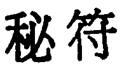
\includegraphics{figures/fig-10.jpg}

Мучительно сознавая, что чудом остался цел, Кантрелл хрипло продолжает:

--- Мы подумали, что вы захотите увидеть программу в действии. Сейчас я покажу ее на экране, а в перерыве можете подойти и попробовать самостоятельно.

Рэнди запускает программу. Его компьютер подключен к видеоразъему под столом, так что султанские спецы смогут проецировать то, что видит Рэнди, на небольшой экран в дальнем конце зала. На дисплее --- демоверсия программы электронных расчетов, однако программа <<Фоторобот>> по прежнему работает в фоновом режиме. Рэнди придвигает ноутбук Джону (на жестком диске сейчас должен появиться портрет Джона Кантрелла).

--- Я могу написать лучшую из возможных криптографических программ, но грош ей цена без надежной системы верификации пользователя. --- К Джону отчасти вернулась обычная самоуверенность. --- Как компьютер узнает, что вы --- это вы? Пароль легко угадать, украсть или подделать. Компьютер должен знать о вас что то уникальное, как отпечаток пальца. Обычно ему предлагается взглянуть на какую то часть вашего тела --- например сосуды сетчатки вашего глаза, или услышать отчетливый звук вашего голоса и сравнить с данными, записанными в памяти. Такого рода технология зовется биометрией. В корпорации <<Эпифит>> работает один из лучших в мире специалистов по биометрии. Доктор Эберхард Фёр создал систему распознавания почерка, которая считается непревзойденной. --- Джон некоторое время продолжает панегирик. У Эба и остальных скучающий взгляд --- все читали его резюме. --- Сейчас мы покажем вам распознавание голоса, но программа представляет собой заменяемый модуль, так что можно перейти на другую систему по выбору пользователя, скажем, считывание геометрии руки.

Джон показывает, как работает программа. В отличие от большинства демоверсий она и впрямь работает, а не зависает. Он даже пытается обмануть ее, записав и прокрутив свой голос на приличном портативном магнитофоне. Однако программу не проведешь. Это впечатляет китайцев. До сих пор они выглядели как содержимое контейнера за музеем восковых фигур после выставки, посвященной Культурной революции.

Не все такие маловеры. Гарвард Ли --- целиком на стороне Джона Кантрелла, а филиппинский тяжеловес, похоже, спит и видит, как бы вложить свои деньги в Крипту.

Перерыв! Двери распахиваются. За ними обеденный зал с буфетной стойкой у дальней стены --- оттуда тянет запахами карри, кайенского перца, чеснока и бергамота. Дантист садится за один стол с эпифитовцами, но почти не разговаривает, а сидит с постной миной, смотрит, жует и думает. Когда Ави спрашивает о его впечатлениях, Кеплер спокойно отвечает: <<Встреча была информативная>>.

Три грации эпилептически дергаются. Очевидно, в словаре Дантиста <<информативная>> --- исключительно бранное слово. Оно означает, что Кеплер узнал на встрече нечто такое, чего не знал, когда туда направлялся. В его системе ценностей это непростительное упущение разведки.

Мучительная тишина. Потом Кеплер говорит:

--- Однако не лишенная интереса.

Белозубые ассистентки испускают глубокий вздох. Значит, Кеплер досадует, что его держали в неведении, но одновременно почуял новые деловые возможности. Интересно, что хуже: подозрительность Дантиста или его алчность? Скоро выяснится. Рэнди, с его дурацкой откровенностью, едва не ляпает: <<Для нас встреча тоже была информативной>>, но сдерживается, заметив, что Ави этого не сказал. Прибыли акционеров такие слова не увеличат. Лучше не показывать карты, пусть Кеплер гадает, знали они наперед или нет.

Рэнди выбрал место так, чтобы видеть в открытую дверь конференц зал и свой ноутбук. Один за другим члены других делегаций заходят в зал и запускают демоверсию: записывают свой голос и смотрят, как он распознается. Некоторые особо продвинутые набирают команды на клавиатуре, может быть, даже ps. Хотя у Рэнди все настроено так, что сильно не напортишь, ему больно видеть, как чужие люди тычут пальцами в его клавиатуру.

Это ощущение грызет Рэнди всю вторую половину встречи, посвященную связи Кинакуты с остальным миром. Ему бы слушать, потому что разговор касается, в частности, филиппинского проекта. Но он не слушает, а изводится из за клавиатуры, заляпанной чужими пальцами, потом из за того, что это его так сильно задело, а значит --- бизнесмен из него никудышный. Клавиатура, строго говоря, не его, а корпорации <<Эпифит>>. Если для увеличения прибыли акционеров надо, чтобы сомнительные азиаты рылись в его файлах, он должен это только приветствовать.

Собрание расходится. Эпифитовцы и японцы обедают вместе, Рэнди устал и рассеян.

Примерно в девять вечера он прощается и уходит в номер, мысленно сочиняя ответ root@eruditorum.org, в том духе, что, мол, потребность велика, и лучше эту нишу займем мы, чем полная и откровенная сволочь. Однако не успевает компьютер загрузиться, как появляется Дантист в белом махровом халате, распространяя запах водки и гостиничного мыла. Он вторгается в ванную Рэнди (нет, акционеров), наливает себе стакан воды. Стоит у окна (оно оплачено акционерами, как и все в номере) и с минуту хмуро взирает на японское кладбище.

--- Вы осознаете, кто эти люди? --- спрашивает он наконец. Биометрический анализ выявил бы в его голосе недоверие, недоумение и, может быть, немного издевки.

А может, он просто пытается взять Рэнди на пушку. Может, он и есть root@eruditorum.org.

--- Да, --- врет Рэнди.

После встречи Рэнди рассказал про <<Фоторобот>>. Ави похвалил его за изобретательность, распечатал снимки на своем принтере и <<Федеральным экспрессом>> отправил сыщику в Гонконг.

Кеплер поворачивается и скептически оглядывает Рэнди.

--- То ли я, ребята, чего то про вас не знаю, --- говорит он, --- то ли вы решили прыгнуть значительно выше головы.

Будь это первая бизнес попытка Рэнди, он бы сейчас наложил в штаны. Будь это вторая попытка --- немедленно уволился бы и завтра утром улетел в Калифорнию. Однако это уже третья и он кое как сохраняет видимость спокойствия. Свет сзади, так что Кеплер, возможно, не очень хорошо видит его лицо. Рэнди выпивает глоток воды и, набрав в грудь воздуха, спрашивает:

--- Каковы перспективы наших отношений в свете сегодняшней встречи?

--- Речь не о дешевых услугах связи для Филиппин --- если такая цель впрямь когда нибудь ставилась, --- мрачно говорит Кеплер. --- Поток данных через Филиппины теперь приобретает совершенно иное значение. Возможности огромные. С другой стороны, у нас серьезные конкуренты: австралийцы и сингапурцы. По силам ли нам конкурировать с ними, Рэнди?

Вопрос прямой и простой, самого опасного свойства.

--- Мы бы не стали рисковать деньгами акционеров, если б считали иначе.

--- Предсказуемый ответ, --- фыркает Кеплер. --- Мы поговорим по настоящему, Рэнди, или пригласим пиарщиков и обменяемся пресс релизами?

В своих прежних бизнес попытках Рэнди бы на этом месте окочурился. Сейчас он говорит:

--- Я не готов обсуждать это.

--- Рано или поздно придется, --- цедит Дантист. Зубы мудрости придется когда нибудь удалить.

--- Естественно.

--- А пока подумайте вот о чем, --- говорит Кеплер, поворачиваясь к двери. --- Что мы можем предложить в плане телекоммуникационных услуг, чтобы обскакать австралийцев и сингапурцев? Потому что по ценам мы с ними конкурировать не можем.

Это третья бизнес попытка Рэнди, и он не выпаливает: избыточность.

--- Мы, разумеется, будем над этим работать, --- говорит он.

--- Звучит, как отповедь. --- Кеплер, ссутулившись, выходит в коридор и, обернувшись, добавляет. --- Встретимся завтра в Крипте. --- Подмигивает. --- Или в Склепе. Или в Роге Изобилия, как там это по китайски.

Ошарашив Рэнди столь неожиданным человеческим проявлением, он идет прочь.


\chapter{ЯМАМОТО}


Тодзё и его свора армейских дебилов фактически сказали ему: <<Расчистил бы ты Тихий океан, а то нам нужен безопасный коридор шириной где нибудь так десять тысяч миль, чтобы осуществить наш планчик по захвату Южной Америки, Аляски и всей Северной Америки к западу от Скалистых гор. Просьба исполнить как можно скорее. А мы пока окончательно разделаемся с Китаем>>.

К этому времени они уже управляли страной. Убили всех, кто мешал, втерлись в доверие к Императору --- попробуй только скажи, что планчик --- дерьмо, что американцы по настоящему разозлятся и сотрут их с лица земли. Адмирал Исороку Ямамото, честный слуга Императора, пораскинул умишком, составил план, отправил пару суденышек через половину земного шара и стер Перл Харбор с лица земли. Подгадал точно к объявлению войны. Сказать по правде, сработал очень даже неплохо.

Позже в кабинет вполз один из адъютантов --- с тем отвратительным раболепным видом, который напускают на себя подчиненные, когда собираются по настоящему испортить тебе настроение, --- и сообщил, что из за неразберихи в вашингтонском посольстве эти остолопы передали декларацию об объявлении войны, когда американский флот уже шел ко дну.

Армейским придуркам хоть бы хны --- промашка вышла, пустяки, с кем не бывает. Исороку Ямамото давно отчаялся объяснить им, что американцы жутко обидчивые. Этого не понять японцам, которые научаются глотать обиды раньше, чем глотать твердую пищу. Даже если объяснить Тодзё и его тупоголовым кретинам, что американцы разозлились, те только посмеются. Ну и что америкашки нам сделают? Запустят в физиономию тортом? Ха, ха, ха! Передайте саке и позовите еще гейшу!

В бытность свою в Америке Исороку Ямамото играл с янки в покер, дымя, как паровоз, чтобы заглушить запах их мерзкого лосьона для бритья. Разумеется, янки чудовищно грубы и неотесанны, не надо быть тонким наблюдателем, чтобы это заметить. Они бессовестно обчищали Ямамото за карточным столом, однако адмирал извлек для себя кое какие полезные сведения: понял, что эти веснушчатые увальни бывают исключительно хитры. Ладно бы грубые и тупые --- этих несложно понять.

Однако сочетание грубости и ума --- невыносимо; вот почему рыжие гориллы отвратительны вдвойне. Ямамото по прежнему пытается внушить свою мысль партнерам по большому японскому плану завоевать весь земной шар от Карачи до Денвера. Многие моряки повидали мир и сами во всем убедились, но армейские лишь резали китайцев и насиловали их женщин. Они думают, америкашки такие же, только более рослые и вонючие. Разуйте глаза, убеждает их Ямамото, Земля не просто большой Нанкин. Будь его воля, он бы издал приказ: каждый армейский офицер на время перестает резать первобытных дикарей в джунглях и отправляется в Тихий океан обменяться парочкой залпов с американским оперативным соединением. Тогда, может быть, они бы поняли, во что вляпались.

Вот о чем думает Ямамото вскоре после рассвета в Рабауле, протискиваясь вместе с ножнами в узкую дверцу бомбардировщика <<Мицубиси G4M>>. Янки зовут самолеты этого типа <<Бетти>>. Удивительная пошлость! Они и свои самолеты называют женскими именами, рисуют голых баб на священных орудиях войны! Будь у американцев самурайские мечи, они, наверное, покрывали бы их лаком для ногтей.

Поскольку самолет --- бомбардировщик, оба пилота втиснуты в кабину над основной трубой фюзеляжа. Нос самолета --- тупой купол металлических конструкций, идущих как параллели и меридианы, трапецоиды между ними закрыты прочным стеклом. Самолет развернут к востоку, стеклянный нос пылает неестественно яркими химическими отблесками зари. У японцев ничего не бывает случайно; надо думать, самолет повернут к Восходящему Солнцу для поднятия боевого духа. Адмирал забирается в кабину и пристегивается в таком месте, чтобы удобно было смотреть через стекло, как взлетает его <<Бетти>> и вторая, адмирала Угаки.

С одной стороны --- бухта Симпсона, одна из лучших якорных стоянок в Тихом океане, асимметричное U в обрамлении четкой решетки улиц, среди которой, как бельмо в глазу, английский крикетный овал. С другой стороны, за хребтом --- море Бисмарка. Где то там покоятся несколько тысяч японских солдат, засоленных в покореженных корпусах транспортных кораблей. Еще несколько тысяч спаслись на спасательных плотах, но все их оружие и припасы пошли ко дну, так что теперь это только лишние рты.

И так уже почти год, с самого Мидуэя, когда американцы не клюнули на обманные маневры Ямамото, указывающие в сторону Аляски, а --- на тебе! --- отправили все оставшиеся авианосцы наперерез его флоту. Черт. Черт. Черт. Черт. Черт. Черт. Черт. Ямамото грызет ноготь на большом пальце, прямо через перчатку.

Теперь эти вонючие мужланы топят все до одного транспорты, которые армия шлет в Новую Гвинею. Дьявол! Их самолеты разведчики повсюду --- всегда появляются в нужное время и --- ату! --- над императорскими конвоями смыкаются кровавые клещи <<конфедератов>>.

Два самолета летят на юго восток, над оконечностью Новой Ирландии, к Соломонову морю. Впереди разбросаны Соломоновы острова --- мохнатые нефритовые кочки посреди океана, в шести тысячах пятистах футах внизу. Две кочки поменьше, одна побольше. Место их следующей посадки --- Бугенвиль.

Необходимо совершать инспекционные облеты, поднимать боевой дух на передовой. У Ямамото есть дела поважнее, поэтому он старается уложить в один день как можно больше неизбежных мероприятий. На прошлой неделе он оставил свою флотскую цитадель на острове Трук и вылетел в Рабаул, чтобы на месте руководить боевой операцией: волной массированных авианалетов на американские базы от Новой Гвинеи до Гуадалканала.

Воздушные налеты вроде бы успешны. Уцелевшие пилоты докладывают о большом количестве потопленных кораблей, о целых американских эскадрильях, уничтоженных прямо на взлетной полосе. Ямамото заранее знает, что все эти донесения на поверку окажутся непомерным бахвальством. Большая часть самолетов не возвращается --- американцы вместе со своими не менее гнусными родичами, австралийцами, хорошо подготовились к налетам. Однако и в армии, и на флоте полно честолюбцев, которые из кожи вон лезут, чтобы преподнести Императору хорошие новости, пусть даже и не совсем правдивые. В итоге Ямамото недавно получил поздравительную телеграмму от самого государя. Его долг --- облететь на <<Бетти>> расположение войск, помахать в воздухе священной телеграммой, передать бойцам благословение Императора.

Ноги болят адски. У Ямамото, как у всех остальных в радиусе тысячи миль, тропическая болезнь --- в данном случае бери бери. Это бич японцев и особенно моряков, потому что они едят слишком много очищенного риса, слишком мало рыбы и овощей. Нервные волокна изъедены молочной кислотой, поэтому руки дрожат. Слабое сердце недостаточно сильно гонит кровь, и ноги отекают. Ему надо несколько раз в день менять обувь, но здесь слишком тесно --- мешает не только фонарь кабины, но и меч.

Они приближаются к воздушной базе Императорских военно морских сил на острове Бугенвиль точно по расписанию, в 9.35. Сверху проносится тень; Ямамото, подняв глаза, видит в опасной близости самолет сопровождения. Кто этот кретин? Тут перед глазами возникает зеленый остров и синий океан: <<Бетти>> входит в крутое пике. Другой самолет проносится с ревом, заглушающим моторы <<Бетти>>, и хотя это лишь стремительный росчерк, мозг фиксирует странный двухвостый силуэт: П 38 <<Лайтнинг>>. Насколько адмиралу Ямамото известно, на вооружении японских ВВС таких нет.

По рации доносится голос адмирала Угаки из второй <<Бетти>>, летящей у них в хвосте: он приказывает летчику Ямамото держать строй. Впереди только волны, бьющиеся о берег Бугенвиля, да стремительно приближающаяся зеленая стена леса. Ямамото моряк, а не летчик, но даже он знает: если во время боя не видишь перед собой самолетов, значит, плохи твои дела. Алые вспышки прочерчивают небо и уходят в туманные джунгли, <<Бетти>> начинает сильно дрожать. Периферическое зрение наполняется желтым светом: горит мотор. Пилот держит курс прямо на джунгли: то ли самолет потерял управление, то ли летчик уже убит, то ли его гонит атавистический инстинкт --- скрыться, скрыться среди деревьев!

Они на горизонтальном полете входят в джунгли и на удивление долго летят, прежде чем во что нибудь врезаться. Потом самолет с размаху ударяет в ствол красного дерева, как раненая ласточка --- в бейсбольную биту, и Ямамото ясно --- это конец. Фонарь вокруг адмирала разваливается, меридианы и параллели ломаются и гнутся, но это уже не самое страшное, потому что весь самолет объят пламенем. Кресло выпадает из разбитого купола и летит в пространство. Ямамото стискивает меч, чтобы не выронить священный клинок, не опозорить себя в последние мгновения жизни. Одежда и волосы в огне: он метеором летит через джунгли, сжимая меч своих предков.

Внезапно он кое что понимает. Американцы совершили невозможное, взломали их коды. Это объясняет Мидуэй, объясняет море Бисмарка, Холландию, все. Это объясняет, почему адмирал Ямамото, вместо того чтобы пить зеленый чай и упражняться в каллиграфии под сенью прохладного сада, летит через джунгли со скоростью сто миль в час, преследуемый тоннами горящего металлолома. Надо сообщить, чтобы сменили коды!.. Вот о чем он думает, прежде чем врезаться головой в стофутовый ствол Octomelis sumatrana.


\chapter{АНТЕЙ}


Когда Лоуренс Притчард Уотерхауз впервые за несколько месяцев вступает на священный берег Альбиона, он с изумлением видит повсюду слабые намеки на весну. Местные жители выставили вдоль набережной вазоны с какой то докембрийской декоративной капустой. Зрелище не греет душу, однако придает местности мрачно друидический вид. Впечатление, что видишь отголоски некой культурной традиции, из которой вдумчивый антрополог способен вывести существование настоящих деревьев и лугов значительно дальше к югу. Здесь их заменяют лишайники, которые, поддавшись общему духу, оделись в лиловато серое и зеленовато серое многоцветье.

Они со старым приятелем вещмешком тузят друг друга до самого вокзала и занимают место в <<кукушке>> на Манчестер. Часа два она разводит пары, и у Лоуренса есть время подумать.

Он работает над задачей из области теории информации, возникшей недавно\footnote{После того как раскололи четырехдисковую <<Энигму>>.} в результате желания американского и английского флотов усеять атлантическое дно разбомбленными и торпедированными <<коровами>>. Это толстые немецкие подводные лодки, наполненные топливом, провиантом и боеприпасами. Они болтаются в Атлантике, редко выходят на радиосвязь и служат плавучими базами снабжения, чтобы боевым подлодкам не возвращаться в порт для заправки и пополнения припасов. То, что их усиленно топят, хорошо для конвоев, но наверняка насторожит таких, как Рудольф фон Хакльгебер.

Обыкновенно, исключительно для проформы, союзники посылают самолет разведчик, который якобы случайно обнаруживает <<корову>>. Однако немцы, если отбросить их политическую слепоту, ребята башковитые и когда нибудь уловку разгадают. Если мы и дальше хотим топить их <<коров>>, нам нужно более убедительное оправдание.

Уотерхауз сочинял оправдания весь конец зимы --- начало весны и порядком притомился. Чтобы сочинять их грамотно, нужен математик, хотя задача не вполне математическая. Слава богу, ему хватило ума переписать шифровки из сейфа. Только на них он и держится.

В каком то смысле это пустая трата времени: оригиналы давно переправлены в Блетчли парк, где их наверняка расшифровали в первые же часы. Уотерхауз делает это не столько для победы над врагом, сколько чтобы не разучиться думать и может быть, добавить несколько страниц к новому изданию <<Криптономикона>>. Добравшись до Блетчли, он поспрашивает и выяснит, что же было в этих шифровках.

Обычно он не опускается до жульничества, но листки с U-553 совершенно поставили его в тупик. Они зашифрованы не с помощью <<Энигмы>>, однако расколоть их по крайней мере так же трудно. Обычно начинают с того, что по определенным признакам устанавливают, например, что это шифр перестановки или замены, дальше, скажем, что это апериодический шифр перестановки, в которой ключевые элементы постоянной длины используются для шифровки переменных по длине групп открытого текста, или наоборот. Как только ты классифицировал алгоритм, ты понимаешь, как взламывать код.

Уотерхауз не добрался даже до этой стадии. Он сильно подозревает, что сообщения закодированы с помощью одноразового шифрблокнота. Если так, их не прочтут даже в Блетчли парке, разве что добудут экземпляр шифрблокнота. Он почти надеется услышать, что так оно и есть, и больше не биться головой в каменную стену.

В определенном смысле такой результат означал бы больше вопросов, чем ответов. Немцы считают <<Тритон>> --- четырехдисковую <<Энигму>> --- абсолютно надежной шифровальной машиной. Если так, зачем капитану U-553 понадобился отдельный шифр для каких то сообщений?

Паровоз начинает тарахтеть, как Палата Лордов. Обитатели Внутреннего Йглма выходят из вокзала и занимают места. По вагону идет старикан, продает вчерашние газеты, курево, леденцы. Уотерхауз покупает всего понемногу. Поезд трогается. Взгляд Уотерхауза падает на аршинный заголовок во вчерашней газете: <<В ТИХОМ ОКЕАНЕ СБИТ САМОЛЕТ ЯМАМОТО. АРХИТЕКТОР ПЕРЛ ХАРБОРА ПРЕДПОЛОЖИТЕЛЬНО ПОГИБ>>.

--- Допрыгались, --- бормочет Уотерхауз и, прежде чем читать дальше, распечатывает пачку сигарет. Такое дело надо основательно перекурить.


Тонны смолы и никотина спустя Уотерхауз сходит с поезда и шагает из вокзала станции <<Блетчли парк>> в исключительно яркий весенний день. Перед вокзалом цветут цветы, дует теплый южный ветер. Уотерхаузу тошно идти в душный корпус, однако он идет и слышит там, что никому в данный момент не нужен.

Посетив еще несколько корпусов по разным делам, он сворачивает на север, проходит три мили и открывает дверь кабачка <<Корона>>. Здешняя хозяйка, миссис Рамшо, последние три года успешно привечает у себя бездомных кембриджских математиков.

Доктор Алан Матисон Тьюринг расположился за столиком у окна на двух или трех стульях. Поза с виду исключительно неудобна, но, надо полагать, весьма практична. На столике непочатая кружка чего то красновато бурого; Алан слишком занят, ему не до пива. В сигаретном дыму прорисован призматический столб света, падающий на огромную книгу. Алан держит ее одной рукой, другая прижата ко лбу, как будто информация поступает со страниц в мозг напрямую, минуя промежуточные стадии. Сигарета зажата между пальцами, столбик пепла опасно навис над темными волосами. Глаза застыли, не смотрят в книгу, устремлены куда то в даль.

--- Изобретаем новую машину, доктор Тьюринг?

Глаза обретают подвижность и поворачиваются на голос.

--- Лоуренс, --- тихо говорит Алан, идентифицируя лицо. Потом, душевнее: --- Лоуренс! --- Он с обычной живостью вскакивает и протягивает руку. --- Какая чудесная встреча!

--- Рад тебя видеть, Алан. --- Уотерхауз, как всегда, приятно удивлен, насколько живо и остро Алан на все реагирует.

Еще он тронут искренней приязнью Алана. Алан нелегко сходится с людьми, но уж если дружит, как с Уотерхаузом, то без всякой оглядки на американские или гетеросексуальные представления о мужской сдержанности.

--- Ты что, шел пешком от самого Блетчли? Миссис Рамшо, обслужите!

--- Да тут всего три мили, --- говорит Уотерхауз.

--- Садись. --- Алан внезапно замирает, хмурится и озабоченно глядит на Уотерхауза. --- Откуда ты знаешь, что я изобретаю новую машину? Догадался, исходя из прошлых наблюдений?

--- По тому, что ты читаешь. --- Уотерхауз указывает на книгу. --- <<Справочник по радиолампам>>.

Алан хлопает глазами.

--- Мы с ней неразлучны. Ты должен изучить радиолампы, Лоуренс! Без них твое образование неполно. Только подумать, сколько лет я убил на шестеренки ! Господи!

--- Ты про свою машину для дзета функции? --- спрашивает Лоуренс. --- По моему, она была прекрасна.

--- Как многие другие музейные

экспонаты, --- говорит Алан.

--- Это было шесть лет назад. Ты вынужден был обходиться имеющимися технологиями.

--- Ах, Лоуренс! Ты меня удивляешь! Если на создание машины по имеющейся технологии уходит десять лет, а по новой --- только пять и нужно всего два года на разработку новой технологии, можно уложиться в семь лет, если начать с разработки.

--- Убедил.

--- Вот она, новая технология. --- Алан демонстрирует справочник, словно Моисей --- Скрижали Завета. --- Хвати у меня духа ее использовать, я бы построил машину для дзета функции куда раньше, да и другие в придачу.

--- Что за машину ты придумываешь теперь? --- спрашивает Лоуренс.

--- Я играю в шахматы с неким Дональдом Мичи --- и постоянно проигрываю. Однако человек всегда создавал орудия, чтобы расширить свои возможности. Почему бы не построить машину, которая помогает играть в шахматы?[Алан Тьюринг очень любил шахматы, но, несмотря на все свои невероятные усилия и гигантский интеллект, оставался довольно посредственным шахматистом. Вскоре после окончания войны он написал алгоритм, с помощью которого можно было бы обучить машину игре в шахматы. Поскольку на тот момент еще не существовало компьютера, способного выполнять подобные алгоритмы, он решил сам выступить в этой роли. Следуя своим же инструкциям, Тьюринг действовал как <<человек компьютер>>, и у него уходило более получаса на то, чтобы совершить один ход.

Дональд Мичи (р. 1923) --- английский криптограф, работал вместе с Тьюрингом и Джеком Гудом над <<Колоссом>> и предложил способ программирования этой машины.]

--- А у Дональда Мичи тоже будет машина?

--- Пусть изобретет свою! --- возмущается Алан.

Лоуренс внимательно оглядывает паб. Других посетителей нет, и трудно поверить, что миссис Рамшо --- шпионка.

--- Не имеет ли это отношения к... --- Он кивает в сторону Блетчли парка.

--- Они строят --- я помогал им строить --- машину под названием <<Колосс>>.

--- Мне сразу подумалось, что это твой почерк.

--- Она основана на старых идеях, тех, что мы обсуждали в Нью Джерси, --- говорит Алан. Тон резкий, лицо мрачное. Одной рукой он прижимает к сердцу справочник, другой чиркает в блокноте. Уотерхауз думает, что справочник, как ядро на цепи, тянет Алана назад. Работая с чистыми идеями, как положено математику, он бы двигался со скоростью мысли. Однако Алан увлечен воплощением математических идей в физическом мире. Математика, описывающая Вселенную, --- как свет, бьющий в окно. Алан выпускает сигаретный дым, чтобы свет стал видимым. Он сидит на лугу, глядит на цветы и шишки, выводит математические закономерности их структуры и грезит об электронных ветрах, реющих между анодами и катодами радиоламп; ветры то затихают, то усиливаются, запечатлевая нечто, происходящее у него в мозгу. Тьюринг не смертный и не бог. Он --- Антей. В том, что он соединяет математику с физическим миром, --- его сила и его слабость.

--- Что такой мрачный? --- спрашивает Алан. --- Над чем работаешь?

--- Те же идеи в другом контексте. --- В нескольких словах Уотерхауз итожит все, что сделал за это время для победы. --- По счастью, я набрел на что то по настоящему занятное.

Алан сразу приободряется, как будто последние десять лет в мире не было ничего занятного и Уотерхауз чудом наткнулся на такую диковину.

--- Рассказывай.

--- Криптоаналитическая задача. Не <<Энигма>>. --- Он рассказывает про листки с U-553. --- Сегодня утром я заглянул в Блетчли парк и выяснил, что они все это время бьются над ней так же безрезультатно.

Алан разочарован.

--- Должно быть, одноразовый шифрблокнот. --- В голосе сквозит укоризна.

--- Нет. Шифртекст не лишен закономерностей, --- говорит Уотерхауз.

--- Н да? --- отзывается Алан, встрепенувшись.

--- Я искал закономерности по обычной методике <<Криптономикона>>. Ничего определенного --- просто намеки. В отчаянии я решил начать с чистого листа. Думать, как Алан Тьюринг. Обычно мы стараемся свести задачу к числам, а потом бросить на нее всю мощь математического анализа. Так что я стал переводить сообщения в цифры. Обычно это произвольный процесс. Присваиваешь каждой букве численное значение, как правило, от нуля до двадцати пяти, потом сочиняешь некий произвольный алгоритм, который превращает ряды маленьких чисел в большие. Однако это сообщение иного рода --- в нем использованы тридцать два символа --- степень двойки; у каждого символа есть единственное двоичное представление в пять разрядов длиной.

--- Как в коде Бодо\footnote{Код Бодо (международный телеграфный код) используется в телетайпах.  Каждому из тридцати двух символов, включающих буквы и специальные знаки, присвоен определенный номер. Этот номер может быть представлен в виде пятизначного двоичного числа, то есть пятью нулями или единицами, а также (что практичнее) пятью пробитыми либо непробитыми дырочками в бумажной ленте. Кроме того, эти числа можно выразить чередованием плюсовых и минусовых электрических сигналов, которые передаются по проводам или через радиоволны и распечатываются на другом конце. В последнее время немцы используют зашифрованные телеграфные сообщения для связи между высокими командными постами, например, Берлином и штабами различных армейских соединений. В Блетчли парке эта категория шифров зовется <<Рыба>>; <<Колосс>> строят специально для их расшифровки.}, --- говорит Алан. Он вновь проявляв сдержанный интерес.

--- Поэтому я перевел каждую букву в число от одного до тридцати двух по коду Бодо. У меня получились длинные ряды маленьких чисел. Однако я хотел перевести все числа ряда в одно большое, просто чтобы узнать, есть ли в нем интересные закономерности. Но это проще пареной репы! Если первая буква R код Бодо для нее --- 01011, а вторая --- F, и для нее код --- 10111, то я могу просто составить их в десятизначное двоичное число 0101110111. Потом могу взять код следующей буквы, приставить его сзади и получить пятнадцатизначное число. И так далее. Буквы написаны группами по пять --- двадцатипятизначное двоичное число на группу. Шесть групп в строке --- сто пятьдесят двоичных разрядов на строку. Двадцать строк на странице, всего три тысячи двоичных цифр. То есть о каждой странице можно думать не как о ряде из шестисот букв, но как о закодированном представлении одного числа, порядка двух в трехтысячной степени, или примерно десяти в девятисотой.

--- Ладно, --- говорит Алан. --- Согласен, что использование тридцатидвухбуквенного кода предполагает двоичную схему шифровки. Согласен и с тем, что такая схема позволяет слить пятерки двоичных чисел в более длинные и даже, если идти до конца, слить все двоичные знаки на странице в одно исключительно большое число. Но что это дает?

--- Не знаю, --- сознается Уотерхауз. --- Просто я интуитивно чувствую, что мы имеем дело с новой схемой шифровки, основанной на чисто математическом алгоритме. Иначе какой смысл переходить на тридцатидвухбуквенный алфавит? Подумай: тридцать две буквы годятся и даже необходимы для телетайпа, поскольку там нужны специальные символы, вроде возврата каретки или перевода строки.

--- Ты прав, --- говорит Алан, --- очень странно, что они используют тридцать две буквы в схеме, которая явно шифруется с помощью карандаша и бумаги.

--- Я тысячу раз прокручивал это в голове, --- произносит Уотерхауз, --- и вижу единственное объяснение: они переводят сообщение в большие двоичные числа и комбинируют с другими двоичными числами --- скорее всего одноразовым шифрблокнотом.

--- Тогда ты ничего не добьешься, --- говорит Алан. --- Одноразовый шифрблокнот взломать нельзя.

--- Это верно, --- возражает Уотерхауз, --- только если шифрблокнот действительно случайный. Если для трехтысячезначного числа три тысячи раз бросают монетку и пишут единицу для орла и ноль для решки, то он случайный и абсолютно стойкий. Однако не думаю, что здесь так.

--- Почему? В их шифрблокнотах закономерности?

--- Может быть. Только намеки.

--- Так почему ты думаешь, что они не случайны?

--- Иначе нет смысла изобретать новую схему, --- говорит Уотерхауз. --- Все всю жизнь пользуются одноразовыми шифрблокнотами. Давно прописано, как их составлять. Нет никакого резона в разгар войны переходить на новую, исключительно странную систему.

--- Так в чем, по твоему, ее смысл? --- Алан явно забавляется.

--- Неудобство одноразового шифрблокнота в том, что надо составить два экземпляра и переправить их отправителю и получателю. Положим, ты в Берлине и хочешь послать сообщение кому то на Дальнем Востоке! На подлодке, которую мы нашли, был груз --- золото и много всего другого --- из Японии. Представляешь, какая морока для Оси.

--- Ага. --- До Алана наконец дошло. Однако Уотерхауз все равно заканчивает мысль:

--- Предположим, ты нашел математический алгоритм для генерации очень больших случайных чисел --- во всяком случае, таких, которые выглядят случайными.

--- Псевдослучайных.

--- Да. Разумеется, ты должен хранить алгоритм в тайне. Но если ты передаешь его --- алгоритм то есть --- на другой край света своим адресатам, они смогут с этого дня сами выполнять вычисления и получать шифрблокноты конкретного дня или чего там еще.

По веселому лицу Алана пробегает тень.

--- Однако у немцев уже есть <<Энигма>>. Зачем утруждать себя новой схемой?

--- Может быть, --- предполагает Уотерхауз, --- некоторые немцы не хотят, чтобы весь немецкий флот читал их переписку.

--- M м, --- говорит Алан. Похоже, последние преграды рухнули. Теперь он воплощенная решимость. --- Покажи сообщения!

Уотерхауз открывает портфель, в засохших брызгах и потеках морской воды от путешествия на Йглм и обратно, вытаскивает два больших конверта.

--- Здесь копии, которые я снял, прежде чем отправить оригиналы в Блетчли парк. --- Он похлопывает по одному. --- Они куда разборчивее оригиналов, --- похлопывает по другому, --- которые мне любезно одолжили, чтобы я мог изучить их еще раз.

--- Покажи оригиналы! --- требует Алан.

Уотерхауз толкает через стол второй конверт, покрытый штампами СОВСЕКРЕТНО.

Алан нетерпеливо разрывает конверт, выдергивает листки, раскладывает по столу. У него отвисает челюсть.

В первый миг Уотерхауз думает, что его друг неким олимпийским озарением расшифровал листки с первого взгляда.

Однако это не так. Алан совершенно ошарашен.

--- Я знаю почерк.

--- Да ты что?

--- Видел его тысячу раз. Эти страницы написаны нашим старым другом по велосипедным прогулкам, Рудольфом фон Хакльгебером. Руди написал эти страницы.


Всю следующую неделю Уотерхауз мотается на заседания в Бродвей билдингс. Всякий раз, как должны прийти штатские (особенно --- с аристократическим прононсом), перед началом заседания появляется Чаттан и жутко бодро велит Уотерхаузу молчать в тряпочку, если только не зададут математический вопрос. Уотерхауз не в претензии. Его это вполне устраивает, потому что оставляет время для более важных занятий. На последнем заседании в Бродвей билдингс он доказал теорему.

Примерно за три дня Уотерхауз вычисляет, что в самих заседаниях нет никакого смысла --- обсуждения явно не могут ни во что вылиться. Он даже пытается доказать это с помощью формальной логики, но не силен в ней и знает слишком мало аксиом, чтобы достичь Q.E.D.

Впрочем, к концу недели он заключает, что все эти заседания --- одно из следствий гибели Ямамото. Уинстон Спенсер Черчилль носится с Блетчли парком как курица с яйцом, однако перехват адмиральского самолета пробил заметную брешь в завесе секретности. Головотяпы, допустившие этот промах, пытаются спасти положение, распространяя байку о туземных лазутчиках, которые якобы проведали о полете и сообщили по рации на Гуадалканал, откуда и взлетел роковой П 38. Однако баков П 38 еле еле хватает на полет туда обратно, значит, время взлета было рассчитано тютелька в тютельку. Если у японцев на плечах голова, а не кочан капусты, они не клюнут на эту сказочку. Уинстон Черчилль рвет и мечет, и все эти заседания --- попытка его умиротворить и выдумать какой то разумный поворот в политике.

Каждый вечер после заседания Уотерхауз едет на метро до Юстона, потом на поезде до Блетчли и допоздна сидит над шифрами Руди. Алан работает над ними днем, так что вместе они бьются над задачей почти круглые сутки.

Не все загадки математические. Например, какого дьявола немцы усадили Руди писать длинные числа? Если буквами и впрямь закодирована длинная последовательность цифр, значит, доктору Рудольфу фон Хакльгеберу отведена роль заурядного писаря. Трудно поверить, что хоть одна бюрократическая система способна на такую несусветную глупость. Кроме того, судя по скудным разведданным из Германии, Руди на самом деле занимает значительный пост --- настолько значительный, что его работа полностью засекречена.

Алан предполагает, что Уотерхауз исходит из понятного, но абсолютно ложного допущения. Числа --- не шифртекст, а скорее одноразовый шифрблокнот, с помощью которого капитан U-553 должен был кодировать определенные сообщения, слишком секретные, чтобы пускать их по обычным каналам <<Энигмы>>. Эти одноразовые шифрблокноты по какой то причине составил Руди.

Обычно составление одноразовых шифрблокнотов --- такое же примитивное занятие, как и шифрование, работа для писарей, которые выбирают случайные буквы с помощью лототрона или стопки карточек. Однако Алан и Уотерхауз исходят из допущения, что столкнулись с совершенно новым изобретением, возможно, созданным Руди, и шифрблокнот генерируется не случайным образом, а по какому то математическому алгоритму.

Другими словами, это какие то вычисления, какая то формула, которую придумал Руди. Задаешь некий параметр --- вероятно, дату, возможно, какие то другие данные, скажем, произвольную ключевую фразу или число. Проводишь последовательные вычисления и получаешь девятисотзначное число, то есть три тысячи двоичных знаков, что при переводе в код Бодо дает шестьсот букв (достаточно, чтобы исписать лист бумаги). Девятисотзначное десятичное число, трехтысячезначное двоичное и шестьсот букв --- одно и то же абстрактное, чистое число в разных представлениях.

Тем временем твой адресат, возможно, на другом краю света выполняет те же вычисления, получает тот же одноразовый шифрблокнот и может раскодировать твое сообщение.

Если Тьюринг и Уотерхауз поймут, как вычисляется число они тоже смогут его прочесть.


\chapter{ПЕРЕХВАТ}


Дантист ушел, дверь заперта, телефон выдернут из розетки. Рэндалл Лоуренс Уотерхауз лежит голый на крахмальной простыне поверх непомерно большой кровати. Голова подперта подушкой, чтобы между раздвинутых ступней видеть телевизор: идет выпуск всемирных новостей Би би си. Десятидолларовое пиво из мини бара под рукой. В Америке шесть утра, и, чем смотреть профессиональный баскетбол, он переключился на новости. Выпуск почти целиком посвящен Южной Азии. Материал о тайфуне, который вот вот обрушится на Гонконг, сменяется длинным и трезвым отчетом о нашествии саранчи на индо пакистанской границе. Король Таиланда потребовал, чтобы несколько наиболее коррумпированных чиновников буквально простерлись перед ним ниц. Азиатские новости всегда граничат с фантастикой, но все это на полном серьезе, без всяких тебе кивков и подмигиваний. Теперь рассказывают о заболевании нервной системы в Новой Гвинее, которое передается при употреблении в пищу мозга других людей. Заурядная каннибальская история. Неудивительно, что столько американцев, приехавших сюда по делу, исчезают навсегда --- это все равно что войти на страницы <<Классических комиксов>>.

В дверь стучат. Рэнди встает, надевает бархатный гостиничный халат. Смотрит в глазок, почти ожидая увидеть пигмея с трубочкой отравленных стрел, хотя не отказался бы от соблазнительной восточной куртизанки. Однако это всего лишь Кантрелл. Рэнди открывает дверь. Кантрелл заранее выставил ладони жестом: <<Все, уже заткнулся>>.

--- Не беспокойся, --- предупреждает он. --- О делах говорить не буду.

--- В таком случае я не разобью эту бутылку о твою голову, --- говорит Рэнди. Вероятно, оба чувствуют одно и то же: сегодня слишком много всего произошло, и единственный способ осмыслить события --- не говорить о них. Мозг проделывает большую часть работы в то время, когда его хозяин думает о чем то другом. Поэтому иногда нужно нарочно сочинять посторонние темы для разговора.

--- Идем ко мне в номер, --- говорит Кантрелл. --- У меня Пекка.

--- Финн, которого взорвали?

--- Он самый.

--- А чего он здесь?

--- А чего ему здесь не быть? С тех пор как его взорвали, он ведет технокочевой образ жизни.

--- Это просто совпадение или...

--- Нет, --- говорит Кантрелл. --- Он помогает мне выиграть пари.

--- Какое?

--- Несколько недель назад я рассказал Тому Говарду про ван эйковский перехват. Том ответил, что это сильно смахивает на брехню. Поспорил на десять акций корпорации <<Эпифит>>, что я не смогу это сделать за пределами лаборатории.

--- Пекка в таких вещах сечет?

Вместо того чтобы просто сказать <<да>>, Кантрелл делает серьезное лицо и сообщает:

--- Пекка пишет об этом главу в <<Криптономикон>>. Он считает, что есть лишь один способ обороняться: осваивать технологии, которые могут использовать против нас.

Звучит как призыв к оружию. Отступать стыдно, и Рэнди влезает в брюки, которые так и стоят гармошкой, где он их сбросил, вернувшись от султана. От султана ! По телевизору идет репортаж о пиратах в Южно Китайском море, которые отправляют команду захваченного корабля прогуляться за борт.

--- Весь континент, блин, один сплошной Диснейленд без мер безопасности, --- замечает Рэнди. --- Это только мне кажется сюрреалистическим?

Кантрелл ухмыляется.

--- Если мы начнем про сюрреализм, то закончим сегодняшней встречей.

--- Верно подмечено, --- говорит Рэнди. --- Пошли.


Прежде чем Пекка стал известен в Силиконовой Долине как <<финн, которого взорвали>>, он назывался <<чувак с виолончелью>>, потому что питал к своей виолончели почти аутистскую привязанность, таскал ее повсюду и все время старался запихать в верхнюю багажную сетку. Без всякой связи, его специальностью было радио, и занимался он аналоговыми штучками.

Когда пакетная радиосвязь стала серьезной альтернативой посылке данных по проводам, Пекка переехал в Менло парк и основал фирму, оборудование для которой закупил на компьютерной барахолке. Так Пекка обзавелся девятнадцатидюймовым MultiSync монитором с высоким разрешением, как раз под свои молодые глаза (ему было тогда двадцать четыре). Монитор он подключил к почти новому пентиуму, до отказа набитому оперативной памятью.

Еще он установил Finux, бесплатную операционку на базе UNIX'a, созданную финнами почти исключительно для того, чтобы показать всем <<какие мы крутые>>, и распространяемую через сеть. Разумеется, Finux удивительно мощный и гибкий; в частности, позволяет контролировать цепь видеосигнала до энной степени, выбирать много разных частот развертки и полос пропускания видеоплаты, если вы таким увлекаетесь. Пекка увлекался и, как многие другие финуксоиды, настроил комп так, чтобы тот показывал уйму крохотных пикселей (помещается много информации, но утомительно для глаз) или меньшее число более крупных пикселей, а также разные промежуточные разрешения. Всякий раз, как он менял разрешение, экран на секунду гас и раздавался щелчок --- пьезокристаллы переходили на другой диапазон частот.

Как то в три часа ночи Пекка переключил режим. Экран погас, щелкнул и взорвался ему в лицо. Передняя часть кинескопа была, естественно, из толстого стекла --- ее осколки вошли Пекке в лицо, тело, торс. Тот самый люминофор, который светился под бегущим электронным лучом, передавая информацию глазам Пекки, теперь впился в его тело. Один осколок уничтожил глаз и остановился, не дойдя до мозга самую малость. Другой перерезал связки, третий просвистел рядом с головой и выкусил аккуратный треугольник из левого уха.

Другими словами, Пекка стал первой жертвой Дигибомбера. Он едва не умер от потери крови, и его друзья евтропийцы несколько дней толклись у больничной койки с баллонами фреона, готовые немедленно приступить к делу, если он умрет. Однако Пекка не умер и вызвал новую шумиху тем, что оказался не застрахован. Местные газеты долго заламывали руки по поводу того, как бедный наивный мальчик из страны бесплатной медицины не нашел в себе духа потратиться на медицинскую страховку. В итоге несколько хайтечных магнатов скинулись на оплату медицинских счетов и компьютерный голосовой аппарат, как у Стивена Хокинга.

И вот теперь Пекка сидит у Кантрелла в номере. Виолончель стоит в углу, в районе кобылки еще видна канифолевая пыль. К стене изолентой приклеены проволочные петли и загогулины. Они тянутся к каким то явно самопальным платам, те, в свою очередь, подключены к ноутбуку.

<<Здравствуй Рэнди поздравляю с успехом>>, --- говорит компьютерно сгенерированный голос, как только за Кантреллом и Рэнди закрывается дверь. Это маленькое приветствие Пекка, очевидно, набрал заранее. Все вполне в порядке вещей, удивляет другое: Пекка думает, что корпорация <<Эпифит>> уже добилась каких то успехов.

--- Как продвигается? --- спрашивает Кантрелл.

Пекка печатает ответ. Потом подносит одну руку к изуродованному уху, а другой жмет на кнопку голосового генератора: <<Он в душе. (И впрямь слышно, как в стене шумят трубы.) Его компьютер излучает>>.

--- Ой, --- удивляется Рэнди. --- Том Говард --- в соседней комнате?

--- Через стенку от нас, --- кивает Кантрелл. --- Я нарочно так попросил, чтобы выиграть пари. Его номер --- зеркальное отражение моего, так что компьютер всего в нескольких дюймах, сразу за стеной. Идеальные условия для ван эйковского перехвата.

--- Пекка, ты прямо сейчас получаешь сигналы с его компьютера? --- спрашивает Рэнди.

Пекка кивает, печатает, жмет кнопку: <<Настраиваю. Калибрую>>. Вводное устройство голосового генератора --- MIDI клавиатура под одну руку, пристегнутая к бедру. Пекка вслепую пробегает по нему пальцами, через несколько мгновений слышится голос: <<Нужен Кантрелл>>.

--- Извини. --- Кантрелл садится рядом с Пеккой. Рэнди некоторое время смотрит им через плечо. Он примерно понимает, что они делают.

Если положить лист белой бумаги на старый могильный камень и провести карандашом черту, вы получите одну горизонтальную линию, где то темнее, где то светлее, однако ничего особенного не означающую. Если провести вплотную вторую черту, и так раз за разом, начнет проступать рисунок. Технарь назвал бы этот процесс разверткой или сканированием. В обычном мониторе --- электронно лучевой трубке --- электронный луч действительно пробегает по стеклу от шестидесяти до восьмидесяти раз за секунду, в дисплее ноутбука, как у Рэнди, ничего по настоящему не бегает, отдельные пиксели включаются и выключаются прямую. Однако процесс развертки все равно имеет место: при этом считывается и отображается на дисплее определенная область компьютерной памяти, называемая экранным буфером. Содержимое экранного буфера должно передаваться на дисплей шестьдесят восемьдесят раз за секунду, иначе (1) экран будет мерцать, (2) изображение --- дергаться.

Компьютер, общаясь с вами, не управляет экраном непосредственно, а манипулирует с битами экранного буфера, зная, что другие подсистемы передадут информацию на реальный дисплей. Шестьдесят восемьдесят раз за секунду система говорит себе: <<Блин, пора обновлять экран>>, лезет в начало буфера --- а это, не забывайте, просто часть памяти --- и считывает первые несколько байтов, определяющих, какого цвета будет пиксель в верхнем левом углу экрана. Информация отправляется тем, кто, собственно обновляет экран, будь то электронный луч или что то такое в ноутбуке. Потом считываются следующие несколько байтов, обычно для пикселя справа от первого, и так до правого края экрана. Проводится первая черта натирки с могильного камня.

Теперь, когда достигнут правый край экрана, в этом направлении пикселей больше нет. Значит, следующие несколько байтов отвечают за крайний левый пиксель второй строки. В электроннолучевой трубке возникает небольшая заминка: луч на правом краю экрана, а его просят нарисовать пиксель на левом краю. Он должен переместиться обратно. Это занимает время --- небольшое, но дольше, чем на переход между соседними пикселями. Называется --- время обратного хода по строке. Так продолжается, пока не будет достигнут последний пиксель в нижнем правом углу и натирка с могильного камня не будет завершена. Однако теперь пора начинать по новой; электронный луч (если он есть) должен скользнуть по диагонали к верхнему левому пикселю. Тут тоже налицо заминка, которая называется временем обратного хода по кадру.

Все это происходит от того, что реальный электронный луч по настоящему движется в электронно лучевой трубке. Для дисплея как в ноутбуке, который Том Говард поставил через стенку от Пекки, такие ограничения вроде бы сняты. Однако тайминг сигнала у такого дисплея все равно взят у электронно лучевой трубки. (Просто потому, что старая технология всем, кому надо, понятна и нормально работает, под нее сделаны и протестированы все программные и электронные технологии, а лучшее враг хорошего, особенно если прибыль у тебя настолько мала, что различить ее можно только с помощью методов квантовой механики, и любые помехи в совместимости подкосят компанию на корню.)

В ноутбуке Тома каждая секунда разделена на семьдесят пять абсолютно одинаковых интервалов, в каждый из которых полностью укладывается натирка с могильного камня плюс время обратного хода по кадру. Как понял Рэнди из разговора Пекки с Кантреллом, они уже установили по идущему через стенку сигналу, что Том настроил дисплей на разрешение 768 строк и 1024 пикселя в строке. Для каждого пикселя из буфера считываются и передаются по проводу на экран четыре байта. (Том выставил максимальное цветовое разрешение. Это значит, что нужно по байту на яркость каждого из основных цветов --- красного, зеленого и синего. Один байт лишний, но его все равно оставляют, потому что компьютеры любят степени двойки, а мощность и быстродействие у них сейчас такие, что лишний байт решительно ничего не меняет.) Каждый байт --- восемь двоичных разрядов или битов, значит, 1024 раза за строку из экранного буфера считываются 4 х 8 = 32 бита.

Неведомо для Тома, его компьютер стоит рядом с антенной. Проволока, которую Пекка прилепил к стене, читает электромагнитные волны, постоянно испускаемые компьютером.

Томов ноутбук продавался как компьютер, а не как радиопередатчик, и может удивить, с какой стати он что то испускает. Дело в том, что компьютеры --- двоичные существа. Всякое общение чипа с чипом, подсистемы с подсистемой внутри машины --- все, что движется по проволочкам, заключенным в плоские ленты, и тонюсеньким металлическим линиям на платах --- состоит из переходов от нуля к единице и обратно. Биты получаются, когда вы меняете напряжение на проволочке туда обратно, от нуля до пяти вольт. В учебниках эти скачки рисуются идеальными прямоугольными импульсами: у вас есть идеально ровная линия при V = 0, представляющая двоичный ноль, потом она прыгает вверх под идеально прямым углом, достигает V = 5, снова поворачивает ровно на девяносто градусов и остается на пяти вольтах, пока не приходит время снова скакнуть на ноль, и так далее.

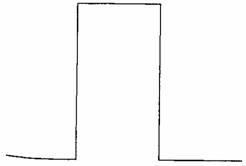
\includegraphics[scale=0.6]{figures/fig-12.jpg}

Это платоновский идеал того, как работает цепь. Однако инженеры вынуждены строить реальные цепи в мрачном аналоговом мире. Куски металла и кремния не способны к платоническому поведению, описанному в книгах. Напряжение и впрямь перескакивает с нуля до пяти вольт, но если проследить за ним на осциллографе, вы увидите, что это не вполне прямоугольный импульс. Вашим глазам предстанет что то примерно такое:

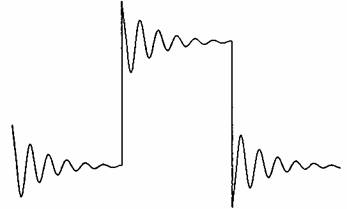
\includegraphics[scale=0.6]{figures/fig-13.jpg}

Затухающие колебания называются звон: переход между двоичным цифрами ударяет по цепи, как било по колоколу. Напряжение прыгает, потом еще некоторое время колеблется возле нового значения. Когда в проводнике вот так колеблется напряжение, значит, в пространство разбегаются радиоволны.

Соответственно каждая проволочка в работающем компьютере --- маленький радиопередатчик. Сигналы, которые она посылает, полностью определяются тем, что происходит в машине. Поскольку проволочек не счесть, а происходит много чего разного, разобрать все радиопередачи со стороны практически невозможно. Большая часть того, что творится в машине, абсолютно неинтересна с точки зрения шпионажа. Однако есть некая последовательность сигналов, которая (1) вполне предсказуема, (2) являет собой именно то, что Пекка хочет увидеть. Это поток битов, считываемых с экранного буфера и отправляемый по проводу экранному железу. В случайном шуме из компьютера время обратного хода по строке и по кадру --- как бой тамтама в густонаселенных джунглях. Теперь, когда Пекка настроится на этот ритм, он сможет ловить излучение кабеля, соединяющего экранный буфер с видеооборудованием, и переводить его обратно в последовательность нулей и единиц, которую можно вывести на собственный монитор. Тогда он увидит то же, что Том Говард, с помощью шпионского метода, называемого ван эйковский перехват.

Все эти общие принципы Рэнди известны. Когда доходит до подробностей, оказывается, что Пекка и Кантрелл выше его на три головы. Через несколько минут ему становится скучно. Он садится Кантреллу на кровать (больше сесть некуда) и обнаруживает на столике наладонник --- включенный, загрузившийся и соединенный с миром телефонным кабелем. Рэнди слышал о таких игрушках. Считается, что это первые сетевые компьютеры, поэтому при включении сразу загружается сетевой браузер. Сетевой браузер --- интерфейс этой машинки.

--- Можно залезть? --- спрашивает Рэнди, и Кантрелл, не обернувшись, отвечает: <<Да>>.

Рэнди заходит на один из больших поисковых сайтов (что занимает примерно минуту, потому что машинка должна сначала войти в сеть) и делает запрос по ключевым словам ((Энди OR Эндрю) Лоуб) AND <<коллективный разум>>. Как всегда, выбрасываются десятки тысяч документов. Однако Рэнди без труда находит существенные.


ПОЧЕМУ ОНСО 9ЕОЗ ЯВЛЯЕТСЯ ВИДНЫМ ЧЛЕНОМ КАЛИФОРНИЙСКОЙ АССОЦИАЦИИ АДВОКАТОВ

ОНСО 11А4 испытывает двоякие чувства по поводу того, что ОНСО 9Е03 (в той мере, в какой он/она воспринимается атомизированным обществом в качестве индивидуального организма) является адвокатом. Без сомнения, противоречивые чувства ОНСО 11А4 вполне нормальны и объяснимы. Часть ОНСО 11А4 ненавидит юристов и юридическую систему в целом, как симптомы последней стадии смертельной болезни атомизированного общества. Другая часть понимает, что болезнь может содействовать оздоровлению мемофонда, убивая старый организм, неспособный к распространению своего мемотипа. Не следует обольщаться: юридическая система в ее современной форме является наихудшей системой решения общественных споров. Она вопиюще дорого обходится и в денежном выражении, и как бессмысленная трата способностей со стороны тех, кто избрал ее в качестве рода деятельности. Однако часть ОНСО 11А4 считает, что целей ОНСО 11А4 можно достичь, обратив наиболее одиозные особенности юридической системы против прогнившего атомизированного общества и таким образом ускорив его крах.


Рэнди щелкает по ОНСО 9Е03 и получает:


ОНСО 9Е03 это ОНСО, которое ОНСО 11А4 определяет произвольным битовым обозначением, в числовом выражении составляющим 9Е03 (в шестнадцатеричном представлении ). Щелкните здесь, чтобы узнать больше о системе битовых обозначений, используемой ОНСО 11А4 для замены устаревшей номенклатурной системы <<естественных языков>>. Щелкните здесь, чтобы обозначение ОНСО 9Е03

автоматически заменялось традиционным (фамилия, имя) при вашем перемещении по сайту.


Щелк.


С этого момента выражение ОНСО 9Е03 будет заменяться выражением Эндрю Лоуб. Предупреждаем: мы считаем такую номенклатуру фундаментально ошибочной и не рекомендуем ее использовать, но предоставляем в качестве услуги для тех, кто посещает наш сайт впервые и не привык мыслить в терминах ОНСО.


Щелк.


Вы щелкнули по Эндрю Лоуб

--- обозначение, которое атомизированное общество присвоило мемому ОНСО 9Е03...


Щелк.


...мемом --- это набор мемов, определяющих физическую реальность ОНСО на углеродной основе. Мемы делятся на две большие категории: генетические и семантические. Генетические мемы это просто гены (ДНК), которые распространяются путем обычной биологической репродукции. Семантические мемы --- это идеи (идеологии, религии, мода и т. п.), распространяемые путем общения.


Шелк.


Генетическая часть мемома Эндрю Лоуб на 99\% идентична последовательности, установленной Проектом Генома Человека. Это не следует понимать как поддержку концепции разделения на виды (согласно которой континуум жизненных форм на углеродной основе может или должен произвольно подразделяться на парадигматические виды) вообще и теории о том, что существует вид под названием Гомо сапиенс, в частности.

Семантическая часть мемома Эндрю Лоуб по прежнему неизбежно заражена многими примитивным вирусоподобными мемами, но они планомерно вытесняются новыми семантическими мемами, изначально генерируемыми в ходе рациональных процессов.


Щелк.


ОНСО означает относительно независимую субобщность. Термин может применяться по отношению к любой сущности, которая, с одной стороны, якобы четко ограничена от остального мира (как, впрочем, и клетки в теле), но, в более общем смысле, неразрывно связана с более крупной общностью (как клетки в теле). Например, биологические сущности, традиционно называемые <<людьми>>, на самом деле всего лишь относительно независимые субобщности социального организма.

В диссертации, написанной под именем Эндрю Лоуб, который теперь обозначается как ОНСО 9Е03, указывается, что даже в умеренных климатических зонах ОНСО 0577, изобилующих водой и пищей, жизнь организмов, обозначавшихся в прежних мемосистемах как Гомо сапиенс, по большей части состояла из попыток съесть другие ОНСО. Такая узкая направленность препятствовала бы образованию высокоорганиэованных мемосистем (а именно цивилизаций в традиционном понимании). ОНСО этого типа могут функционировать на более или менее высоком уровне лишь в меру своей принадлежности к более крупному обществу, наиболее логичной эволюционной формой которого является коллективный разум.


Щелк.


Коллективный разум --- это социальный организм, объединяющий ОНСО, способные вырабатывать семантические мемы (<<думать>>). Это могут быть ОНСО на углеродной или кремниевой основе, которые, вливаясь в коллективный разум отбрасывают независимую личность (та в любом случае иллюзорна). Для удобства составляющим коллективного разума присваиваются битовые обозначения.


Щелк.


Битовое обозначение --- случайная последовательность битов, используемая для однозначной идентификации ОНСО. Например, организму, традиционно обозначаемому как Земля (Терра, Гея), присвоено обозначение ОНСО 0577. Данный сайт поддерживается ОНСО 11А4, который является коллективным разумом. ОНСО 11А4 присваивает битовые обозначения с помощью генератора псевдослучайных чисел. Это отличается от практики, которую применяет самозваный <<коллективный разум>>, именующий себя <<Ист бэйский проект коллективного разума>>, но обозначаемый (в системе, принятой ОНСО 11А4 ) как ОНСО Е772. Этот <<коллективный разум>> возник в результате раскола <<коллективного разума один>> (обозначаемого в системе ОНСО 11А4 как ОНСО 4032 ) на несколько меньших <<коллективных разумов>> (<<Ист бэйский проект коллективного разума>>, <<Сан францисский коллективный разум>>, <<Коллективный разум один А>>, <<Реформированный сан францисский коллективный разум>> и <<Всемирный коллективный разум>>) в результате неразрешимых противоречий между различными семантическими мемами. Один из этих семантических мемов предполагает, что обозначения должны присваиваться по порядку, например, <<коллективный разум один>> должен обозначаться ОНСО 0001 и так далее. Другие считают, что числа должны располагаться в порядке значимости, чтобы, например, ОНСО, традиционно называемое <<планета Земля>>, обозначалось ОНСО 0001. Другие семантические мемы согласны с этим утверждением, но настаивают, что нумерация должна начинаться не с 0001, а с 0000. И среди сторонников 0001, и среди сторонников 0000 имеются разногласия по поводу того, какому ОНСО присваивать первый номер: одни считают, что первым и наиболее важным ОНСО является Земля, другие --- что более крупные единицы (Солнечная система, Вселенная, Бог) являются в некотором роде более всеохватывающими и универсальными.


У машинки есть интерфейс для электронной почты. Рэнди набирает:


Кому: root@eruditorum.org

От: dwarf@siblings.net

Тема: Re (2): Зачем?

Посмотрел сайт. Готов допустить, что Вы --- не ОНСО 9Е03. Подозреваю, что Вы --- Дантист, стремящийся к свободному обмену мнениями. Анонимная, электронно подписанная корреспонденция --- единственный безопасный способ такого обмена.

Если хотите убедить меня, что Вы --- не Дантист, объясните Ваш интерес к строительству Крипты.

Искренне Ваш

--- НАЧАЛО МАССИВА ЭЛЕКТРОННОЙ ЦИФРОВОЙ ПОДПИСИ ОРДО --

(и т. д.)

--- КОНЕЦ МАССИВА ЭЛЕКТРОННОЙ ЦИФРОВОЙ ПОДПИСИ ОРДО --


--- Идут биты, --- говорит Кантрелл. --- У тебя там что нибудь важное?

--- Ничего такого, что было бы жаль бросить.

Рэнди откладывает наладонник. Подходит, встает рядом с Пеккой. На экране у того несколько окон, самое большое и верхнее изображение другого компьютерного дисплея. Это рабочий стол окошками и значками. Причем рабочий стол Windows NT, что примечательно и (для Рэнди) неожиданно, поскольку у Пекки запущен Finux, а не Windows NT.

По рабочему столу Windows NT бегает курсор, вызывает меню нажимает кнопки. Однако рука Пекки не движется. Курсор замирает на значке Microsoft Word, который меняет цвет и разворачивается на все большое окно.


Данная версия Microsoft Word зарегистрирована на ТОМАСА ГОВАРДА.


--- Получилось! --- говорит Рэнди.

--- Мы видим то же, что Том, --- говорит Пекка. Открывается окно нового документа, в нем начинают выскакивать слова.


Пометка для себя: вот пусть <<Письма в Пентхауз>> опубликуют это !

Полагаю, что выпускники и выпускницы высших учебных заведений не такие уж выдающиеся любовники. Мы слишком много об этом думаем. Все должно быть вербализовано. Человек, считающий, что ебля --- это сексуальный дискурс, просто не может быть хорош в постели.

У меня прикол по поводу чулок. Они должны быть гладко черные, желательно со швом сзади. В тринадцать я спер в магазине черные колготки, просто чтобы их трогать. Когда я шел домой с колготками в рюкзачке, сердце у меня бешено колотилось, но волнение от кражи померкло в сравнении с тем, что я испытал, распечатав упаковку и прижав нейлон к пухлым подростковым щекам. Я даже попытался надеть их, на мои то волосатые ноги, но абсолютно ничего не почувствовал. Я не хотел их носить. Я хотел, чтобы они были на ком то другом. В тот день я мастурбировал четыре раза.

Меня это страшно волновало. Я был умненький мальчик. Считается, что умные мальчики --- рационалисты. Поэтому в колледже я придумал рациональное объяснение. У нас в колледже девушки в чулках не ходили, но иногда я бывал в городе, видел, как хорошо одетые сотрудницы фирм идут в черных чулках, и научно изучал их ноги. Я приметил, что, когда чулок растягивается на более широкой части ноги, скажем, на икроножной мышце, он светлеет, как воздушный шарик, когда его надуваешь. Соответственно в более узких местах, например на щиколотке, он темнее. От этого икра кажется полнее, щиколотка --- тоньше. Ноги в целом выглядят более здоровыми, намекая, что между ними можно найти ДНК более высокого класса.

Q.E.D. Мой прикол насчет чулок --- высокоразумная адаптация. Я просто доказал, какой я умный, насколько рациональны даже самые иррациональные части моего мозга. Секс надо мной не властен, мне нечего бояться.

Это были глубоко школьные рассуждения, но в наши дни большинство образованных людей рассуждают, как школьники, до тридцати и позже, так что я надолго на этом застрял. У моей жены Вирджинии, вероятно, были такие же рациональные оправдания ее собственных сексуальных потребностей, о которых я узнал значительно позже. Неудивительно, что наша добрачная половая жизнь была очень так себе. Ни она, ни я в этом, разумеется, не признавались. Иначе я должен был бы признать, что все это --- из за нежелания Вирджинии носить черные чулки, а я слишком хотел быть чутким и современным. Я любил Вирджинию за ее ум. Каким надо быть нечутким извращенцем, чтобы отвергать ее за нежелание натягивать на ноги полупрозрачные нейлоновые трубки? Мне, пухлому школяру, крупно повезло такую заполучить.

На шестом году нашего брака я присутствовал на конференции <<Комдекс>> в качестве президента небольшой высокотехнологической компании. К тому времени я уже был не такой пухлый и не такой школяр. Я познакомился с девушкой из отдела маркетинга крупной сети по распространению программного обеспечения. Она носила гладкие черные чулки. Кончилось тем, что мы трахнулись у меня в номере. Это было что то необыкновенное. Домой я вернулся обескураженный и пристыженный. После этого наша с Вирджинией жизнь совсем разладилась. За два года мы трахнулись раз десять, не больше.

У Вирджинии умерла бабушка, и мы поехали на похороны. Вирджинии пришлось надеть платье, а значит, побрить ноги и натянуть чулки, что с нашей женитьбы случалось всего несколько раз. Я едва не упал, когда ее увидел, и всю заупокойную службу мучился сильнейшей зудящей эрекцией, только и думая, куда бы Вирджинию затащить.

Бабуля жила одна в большом старом доме на холме, пока за пару месяцев до смерти не сломала шейку бедра и не оказалась в больнице. Все ее дети, внуки и правнуки съехались на похороны, так что в доме собралась уйма народу. Дом был красивый и хорошо обставленный. Правда, в последние годы бабулька стала страшной барахольщицей и распихивала повсюду кучи газет, писем и тому подобного. В конце концов мы вывезли несколько грузовиков мусора.

Во всем остальном бабка была очень организованная и оставила весьма подробное завещание. Мебель, посуда, ковры и безделушки --- все это она четко расписала между родней. Добра было много, но и потомков --- целая куча, так что каждому досталось всего ничего. Вирджинии бабка отписала черный комод орехового дерева с зеркалом, стоящий в нежилой спальне. Мы пошли его смотреть, и там то я ее трахнул. Я стоял в спущенных штанах, а она сидела на комоде, и ее обтянутые черными чулками пятки вжимались мне в зад. Это было потрясающе. Хорошо, что родственники внизу ели, пили и разговаривали, не то они услышали бы, как она стонет и вопит.

Я наконец рассказал ей про чулки. Мне сразу полегчало. К тому времени я кое что прочел про то, как развивается мозг, и смирился со своим приколом. Получалось, что в определенном возрасте, где то между двумя и пятью годами, мозг просто застывает. Та часть, которая отвечает за секс, формируется в это время, и дальше ты живешь с ней до конца жизни. Все голубые, с которыми я говорил, утверждают, что осознали себя голубыми, или по крайней мере отличными от других, задолго до того, как начали думать о сексе, и все они согласны, что гомосексуалиста не сделаешь натуралом, и наоборот.

В этом возрасте часть мозга, отвечающая за секс, часто закорачивается на другие, никак не связанные отделы. Тогда то и возникает ориентация на сексуальное подавление или подчинение, а у многих появляются очень специфические приколы --- скажем, по поводу резины, перьев или обуви. Некоторые бедолаги западают на маленьких детей, и тогда пиши пропало --- их можно только кастрировать или запереть до конца жизни. Никакое лечение тут не поможет.

То есть, если хорошенько взвесить, мне достался далеко не худший прикол. Все это я изложил Вирджинии по дороге домой и сам удивился, как спокойно она выслушала. Мне, идиоту, было невдомек, что она размышляет, как это относится к ней самой.

Когда мы вернулись, она честно пошла и купила несколько пар чулок, даже попыталась их носить, но это оказалось не так просто. Чулки предполагают определенный стиль жизни. Они выглядят глупо с джинсами и кроссовками. К чулкам нужны платье или юбка, и не просто джинсовая, а более красивая и парадная. Кроме того, нужны туфли, которых у Вирджинии не было. В чулках неудобно ездить на работу на велосипеде. Более того, чулки нельзя было носить у нас дома. Пока мы учились в аспирантуре, денег не хватало, и мебель мы покупали подержанную, а кое что я сам соорудил из досок. Вся эта мебель оказалась в скрытых заусеницах, которые мы не замечали, пока ходили в джинсах, но чулки о них рвались в первые пятнадцать минут. Аналогично, у нашего недостроенного дома и развалюшной машины оказалась куча острых углов, цепляющих чулки. С другой стороны, когда мы летали в Лондон на юбилей свадьбы, ездили в черных такси, останавливались в хороших гостиницах, ели в дорогих ресторанах, мы целую неделю вращались в мире, идеально приспособленном для чулок. Это показывало, как сильно должна измениться наша жизнь, чтобы Вирджиния начала так одеваться.

Короче, в припадке добрых намерений куча денег была потрачена на чулки. Какое то количество раз мы трахнулись очень даже неплохо, хотя, похоже, удовольствие было больше с моей стороны. Вирджиния ни разу не испытала того звериного экстаза, что на бабулькиных похоронах. Чулки скоро изорвались, новые купить у Вирджинии все как то не получалось, и через год мы вернулись к тому, с чего начали.

Однако наша жизнь понемногу менялась. Я продал кое какие акции, мы купили новый дом на холме. Наняли грузчиков перевезти нашу обшарпанную мебель, которая в новом доме смотрелась еще плачевнее. Вирджиния сменила работу и теперь должна была ездить туда на машине. Я счел, что наша развалюха недостаточно безопасна, и купил ей маленький <<лексус>> с кожаными сиденьями и шерстяным ковриком, без всяких углов и зацепок. Скоро пошли дети, я продал старый пикап и купил минивэн.

Тем не менее меня жаба душила покупать новую мебель, пока не начались проблемы со спиной и я не понял, что все дело в продавленном матрасе, на котором мы спим. Поскольку речь шла о моей спине, я и отправился за покупкой.

Вообще то мне легче прижечь себе язык сигаретой, чем идти что нибудь покупать. Я представил, как буду обходить все большие мебельные салоны, сравнивая кровати, и мне захотелось умереть. Я хотел прийти в одно место, купить и покончить с этим раз и навсегда. Однако я не хотел дерьмовую кровать, на которую через год будет тошно смотреть, или дешевый матрас, который через пять лет промнется и боли в спине начнутся по новой.

Поэтому я направился прямиком в местную галерею <<Гомера Болструда>>. Я слышал, как говорят о тамошней мебели, особенно женщины --- у них сразу становятся такие приглушенные, религиозные голоса. Фабрика, где все это делают, вроде бы в Новой Англии, в том же здании, что и триста лет назад, а стружкой от Гомера Болструда, по слухам, разводили костры под ведьмами. <<Гомер Болструд>> --- вот ответ на вопрос, который я задавал себе с самых похорон: откуда берется вся эта роскошная бабулькина мебель? В каждой семье молодые люди ездят к бабуле на День благодарения и другие нудные семейные торжества, а сами гадают, какой буфет смогут забрать, когда старушка откинет копыта. Некоторые не в силах дотерпеть и отправляются в антикварные магазины.

Однако если запас старинной мебели ограничен, то откуда возьмутся будущие бабули? Я представил, как полстолетия спустя наши с Вирджинией потомки передерутся из за одного черного комода орехового дерева, а всю остальную нашу мебель свезут прямиком на свалку. Поскольку население растет, а запас старинной мебели не увеличивается, такие ситуации неизбежны. Должен быть источник новой бабулькиной мебели, иначе все будущие американцы обречены сидеть в виниловых креслах, из которых сыплется на пол пенопластовая крупа.

Ответ: <<Гомер Болструд>>. Цена высока. Каждый стол и стул от <<Гомера Болструда>> должен бы по хорошему продаваться в коробочке с бархатной подкладкой, как драгоценность. Поэтому я отправился в <<Гомер Болструд>>, ворвался в дверь и налетел на секретаршу. В кроссовках и джинсах я сразу почувствовал себя оборванцем. Видимо, на ее глазах в эту дверь входило много разбогатевших компьютерщиков, потому что она не бухнулась в обморок, а спокойно пригласила пожилую женщину и сказала, что это будет мой личный консультант. Звали ее Маргарет. <<Где кровати?>> --- спросил я. Маргарет поджала губы и объяснила, что это не такое место, где кровати в одном большом зале выставлены рядами, как свиные ноги в мясной лавке. Галерея <<Гомера Болструда>> состоит из шикарно обставленных комнат, в том числе спален, где, кроме всего прочего, есть кровати. Маргарет повела меня их смотреть. По пути из комнаты в комнату я не преминул заметить, что на Маргарет черные чулки с идеально прямым швом.

Мне стало неловко от эротического чувства к Маргарет, и некоторое время я перебарывал желание ляпнуть: <<Просто продайте мне самую большую и дорогую кровать, какая у вас есть>>. Маргарет показала кровати различных стилей. Названия ничего мне не говорили. Одни выглядели современными, другие --- под старину, я указал на очень большую, высокую кровать бабулькиного типа и сказал: <<Беру>>.

Три месяца пришлось ждать, пока ее изготавливали вручную умельцы, работающие по тем же ставкам, что психоаналитики. Потом кровать привезли. Собирали ее рабочие в белых комбинезонах, как в цехе по производству микропроцессоров. Вирджиния вернулась домой с работы. Она была в джинсовой юбке, толстых носках и панталетах. Дети еще не пришли из школы. Мы трахнулись на новой кровати. Надеюсь, я был на должном уровне. Мне не удалось удержать эрекцию и пришлось доводить дело до конца, просунув голову между ее шершавыми бедрами. Хотя уши у меня были зажаты ее ляжками, я все равно слышал, как Вирджиния вопит и стонет. Под конец она забилась в таких судорогах, что чуть не свернула мне шею. Ее оргазм длился полных две или три минуты. Тогда я впервые понял, что Вирджиния может кончить только по соседству с (желательно на) драгоценным предметом мебели, ей лично принадлежащим.


Окно с изображением рабочего стола исчезает. Пекка щелчком отправил его в небытие.

--- Больше не выдержу, --- говорит электронно бесстрастный голос.

--- Предсказываю любовь втроем между Томом, его женой и Маргарет на кровати в мебельном магазине, страниц так через сто, --- задумчиво произносит Кантрелл.

--- Интересно, это Том? Или какой то его вымышленный персонаж? --- говорит Пекка.

--- Означает ли это, что ты выиграл пари? --- спрашивает Рэнди.

--- Только если придумаю, как получить выигрыш, --- отвечает Кантрелл.


\chapter{ВПЛАВЬ}


Над морем Бисмарка сгустились бурые миазмы, пахнущие мазутом и барбекю. Американские торпедные катера вырываются из смрадного тумана, едва касаясь воды корпусом, прочерчивают море изогнутыми шрамами белой пены и выстраиваются для атаки на последние транспорты, покрытые, как замшелая скала, бурым ковром солдат. Торпеды летят, словно стрелы из арбалета, выпущенные сжатым воздухом из труб под корабельными палубами. Они шлепаются в воду, выбирают удобную глубину, где море всегда спокойное, и, таща за собой хвост пузырей, несутся к транспортам. Гото Денго отворачивается и слышит, но не видит взрыв. Почти никто в японской армии не умеет плавать.

Потом самолеты возвращаются и обстреливают их с воздуха. Те, кто умеет нырять и догадывается это сделать, неуязвимы. Других довольно быстро не остается. Самолеты улетают. Гото Денго стаскивает спасжилет с трупа. До вечера еще много часов, а Гото уже обгорел на солнце, как никогда в жизни. Заимствует вдобавок гимнастерку, повязывает ее на голову, как бурнус.

Те, кто еще жив и умеет плавать, стараются сбиться в кучу. Прихотливые течения между Новой Гвинеей и Новой Британией тянут их в разные стороны. Некоторые медленно дрейфуют прочь, пытаясь докричаться до товарищей. В конце концов Гото Денго оказывается на краю тающего архипелага из, может быть, сотни пловцов. Многие цепляются за спасательные круги или доски. Волны гораздо выше головы, так что видно не очень далеко.

Перед закатом марево ненадолго рассеивается. Гото Денго видит солнце и впервые с начала дня понимает, где восток, а где запад. А самое замечательное: он видит над южным горизонтом горы, покрытые голубовато белым льдом.

--- Я поплыву к Новой Гвинее! --- кричит он и начинает грести. Нечего и пытаться обсудить это с другими. Те, кто решает за ним последовать --- в общей сложности, может быть, несколько десятков пловцов, --- тоже принимаются работать руками и ногами. Море, как на удачу, удивительно тихое.

Гото Денго медленно, спокойно плывет на боку. Большинство пловцов барахтаются по собачьи. Продвигаются ли они, сказать нельзя. Когда начинают зажигаться звезды, Гото переворачивается на спину и находит Полярную. Пока плывешь от нее, физически невозможно промахнуться мимо Новой Гвинеи.

Темнеет. Слабо светят звезды и месяц. Пловцы перекликаются, стараясь держаться вместе. Некоторых уносит течением: их слышно, но не видно. Остальные ничем не могут помочь, только слушают затихающие крики.

Акулы появляются около полуночи. Первая жертва --- солдат, раскроивший себе лоб о край люка, когда выбирался с тонущего корабля. За ним с самого утра тянется розовая дорожка крови, она то и вывела акул на пловцов.

Сперва акулы не знают, с кем имеют дело, поэтому постепенно выматывают его, откусывая по кусочку. Поняв, что добыча легкая, они приходят в боевое исступление, тем более фантастическое, что сами акулы скрыты черной водой. Крик обрывается на середине, человек исчезает рывком. Иногда над поверхностью взлетают нога или голова. У воды, захлестывающей в рот, появляется привкус железа.

Атака длится несколько часов. По видимому, шум и запах привлекли несколько конкурирующих стай, потому что временами наступает затишье, затем --- новая бойня. Гото Денго утыкается лицом в оторванный акулий хвост и впивается в него зубами. Акулы едят их --- почему не ответить тем же. В токийских ресторанах за сасими из акулы берут кучу денег. Шкура на хвосте жесткая, но с оторванного края висят клочья мяса. Гото Денго вгрызается в него и уплетает за обе щеки.

У его отца была фетровая шляпа на бежевой шелковой подкладке и трубка, табак для которой приходилось выписывать из Америки. Отец уходил в горы, садился на камень, потуже натягивал шляпу, чтобы ветер не холодил лысину, раскуривал трубку и долго сидел так, просто глядя на мир.

--- Что ты делаешь? --- спрашивал маленький Денго.

--- Созерцаю, --- отвечал отец.

--- Сколько ж можно смотреть на одно и то же?

--- Бесконечно. Вот глянь. --- Отец указывал чубуком. Из мундштука разматывался тонкий белый дымок, словно нить из шелковичного кокона. --- Та полоса темной породы --- рудоносная. Из нее можно добывать медь, может быть, попутно --- свинец и цинк. Можно построить фуникулер вон до того плоского места, потом пройти наклонную штольню параллельно простиранию залежи... --- Денго включался и придумывал, где будут жить горняки, где построить школу, а где разбить площадку для игр. Под конец разговора в долине вырастал воображаемый поселок.

В ту ночь у Гото Денго много времени для созерцания. Он заметил, что на оторванные части тела акулы практически не нападают. Тех, кто плывет быстрее, хватают первыми. Поэтому при появлении акул он неподвижно замирает на спине и не шевелит и мускулом, даже когда зазубренный край чьего то ребра тычет его в лицо.

Наступает рассвет, через сто или двести часов после заката. Гото Денго никогда не бодрствовал целую ночь и потрясен, что такое огромное солнце ушло с одного края планеты и вышло с другой. Он --- вирус, зародыш, живущий на поверхности неизмеримо огромных, стремительно движущихся тел. И, удивительное дело, он по прежнему не один: еще трое пережили ночь и акул. Они подплывают ближе и поворачивают к снежным пикам Новой Гвинеи, нежно розовым в свете зари.

--- Они ничуть не приблизились, --- говорит один.

--- Они в глубине острова, --- объясняет Гото Денго. --- Мы плывем не к горам, а к берегу --- гораздо ближе. Давайте приналяжем, пока не умерли от жажды. --- Он начинает грести на боку.

Один из выживших --- судя по выговору, уроженец Окинавы --- отлично плавает. Они с Гото Денго легко оторвались бы от двух других, однако весь день держатся с ними вместе.

Один из тех, кто плывет медленно, перед этим неделю страдал поносом и, вероятно, уже был обезвожен. Когда солнце зависает прямо над ними, как огнемет, он начинает биться в судорогах, нахлебывается воды и идет ко дну.

Второй медленный пловец --- из Токио. Он в гораздо лучшей физической форме, просто не умеет плавать. <<Самое время научиться>>, --- говорит Гото Денго. Примерно час они с окинавцем учат его грести на спине и на боку, потом возобновляют движение к югу.

Ближе к закату Гото Денго замечает, что окинавец большими глотками пьет морскую воду. Смотреть больно, главным образом оттого, что безумно хочется сделать то же самое. <<Нет! Тебе будет плохо!>> --- говорит он. Голос слабый. Набрать в грудь воздуха, преодолевая безжалостное давление воды --- труд непосильный. Каждая мышца ноет.

К тому времени, когда Гото Денго доплывает до окинавца того уже рвет. С помощью токийца Гото засовывает пальцы ему в глотку и помогает вытошнить остальное.

Парень совсем ослабел, он лежит на спине и бредит. Впрочем, посреди ночи, когда Гото Денго наконец решает его бросить, окинавец внезапно приходит в себя и спрашивает: <<Где Полярная?>>

--- Сегодня облака, --- говорит Гото Денго. --- Но в них белое пятно --- может быть, луна.

Ориентируясь по светлому пятну, они прикидывают, где может быть Новая Гвинея, и плывут дальше. Руки и ноги --- как мешки с глиной; все трое галлюцинируют.

Вроде бы встает солнце. Они в паровой туманности, которая несется через отдаленные части галактики, излучая золотисто розовый свет.

--- Пахнет гнилью, --- говорит один (Гото Денго не может разобрать который).

--- Гангрена? --- предполагает другой.

Гото Денго принюхивается, тратя на это половину оставшихся сил.

--- Не мясо, --- говорит он. --- Растения.

Никто больше не может плыть, а если б и мог, то не знал бы куда --- туман светится равномерно. В любом случае это ничего бы не изменило --- течение гонит их, куда хочет.

Гото Денго некоторое время спит, а может быть --- нет. Нога задевает о какой то выступ. Слава богу. Акулы появились, чтобы их прикончить.

Волны становятся агрессивнее. Нога снова обо что то задевает. Обожженная кожа вопит. Оно твердое и колючее.

Что то торчит из воды прямо впереди, какие то белые бугры. Верхушки кораллов.

Волна разбивается, подхватывает их и тащит через кораллы, обдирая половину кожи. Гото Денго ломает палец и считает, что ему еще повезло. Следующая волна, снимая оставшуюся кожу, выбрасывает его в лагуну. Что то выталкивает ноги вверх, а поскольку все тело --- обмякший мешок с дерьмом, то голова зарывается в воду и лицо втыкается в колкий коралловый песок. Руки и ноги забыли обычные движения, умеют только грести, и проходит некоторое время, прежде чем Гото, упершись в дно, поднимает голову над водой, потом на карачках ползет к берегу. Запах гниющей растительности повсюду, как будто провиант для целой дивизии оставили на неделю под солнцем.

Он находит песок, не залитый водой, поворачивается и садится. Окинавец чуть позади, тоже ползет на карачках. Токиец сумел встать и бредет к берегу, шатаясь под ударами волн. Он смеется.

Окинавец падает на песок рядом с Гото Денго и даже не пытается сесть.

Волна сбивает токийского паренька с ног. Тот со смехом валится в прибой, успевая выставить руку.

Смех резко обрывается. Токиец вскакивает. Что то болтается у него на руке: извивающаяся змея. Он встряхивает ее, как плеть, змея отлетает в воду.

Испуганный, отрезвленный, токиец проходит последние пять шесть шагов и падает ничком. Когда Гото Денго дотягивается до него рукой, он уже мертвее мертвого.

Трудно сказать, как долго Гото Денго собирается с силами. Может быть, он заснул сидя. Парнишка из Окинавы по прежнему лежит и бредит. Гото Денго с усилием встает и, шатаясь, идет на поиски пресной воды.

Это не настоящий берег, просто береговой вал метров десять в длину и, может быть, три в ширину, поросший сверху какой то высокой травой. Дальше начинается стоячая лагуна, стиснутая сплошным переплетением жизни, таким плотным, что пройти там невозможно. Поэтому, невзирая на то, что случилось с токийцем, Гото Денго бредет по лагуне, надеясь выйти к ручью.

Он идет примерно час, но лагуна вновь выводит его к морю. Он сдается и пьет воду, по которой шел, в надежде, что она будет чуть более пресной. Его долго тошнит, но потом, как ни странно, становится чуть легче. Идет в заросли, ориентируясь по шуму прибоя сзади, и примерно через час находит речушку с настоящей пресной водой. Напившись, чувствует в себе силы вернуться за товарищем и, если надо, нести его к ручью на себе.

Гото Денго возвращается на берег. Окинавца нет, но вокруг понатоптано следов. Песок сухой, следы невнятные. Наверное, это патруль! Товарищи узнали о нападении на конвой и прочесывают берег в поисках уцелевших. Где то близко в джунглях должен быть бивуак!

Гото Денго идет по следам. Примерно через милю тропа пересекает мокрый глинистый пятачок, на котором следы отпечатались отчетливо. Все они оставлены босыми ступнями с огромными растопыренными пальцами. Следы людей, никогда не носивших обуви.

Следующие метров сто он продвигается осторожнее. Слышны голоса. В армии их научили, как проникать в джунгли, как бесшумно проползать ночью через вражеские ряды. Разумеется на тренировках в Японии его не жрали заживо москиты и муравьи, но Гото Денго уже почти все равно. За час кропотливого труда он выбирается на открытое место, откуда видна поляна, по которой вьется заболоченный ручеек. Над зловонной жижей высятся на сваях несколько домов, крытых охапками пальмовых листьев.

Прежде чем искать товарища, Гото Денго должен найти еду. Посреди поляны булькает на костре котел с белой кашей, но рядом --- жилистые женщины в одних косматых юбочках, едва прикрывающих срам.

Из некоторых длинных домов тоже поднимается дым. Однако, чтобы попасть туда, надо карабкаться по тяжелой наклонной лестнице и ползком протискиваться в узкий лаз. Ребенок с палкой, встав там, сможет не впустить чужака. Перед некоторыми лазами висят тряпичные узлы (ткани у них, выходит, все таки есть), наполненные чем то круглым --- кокосовыми орехами или другими припасами, подвешенными для защиты от муравьев.

Человек семьдесят собрались посреди поляны вокруг чего то интересного. Они движутся, и Гото Денго временами различает за телами кого то, возможно, японца: он сидит под пальмой, руки связаны за спиной. Лицо в крови, и он не шевелится. Собравшиеся в основном мужчины, почти все --- с копьями. На них тоже юбочки из чего то волокнистого, иногда выкрашенные в зеленый или красный цвет и еле еле прикрывающие половые органы. У тех, кто постарше и покрупнее, на руках повязаны тряпичные полоски, у некоторых лица раскрашены светлой глиной, а в носовые перегородки просунуты различные предметы, иногда довольно крупные.

Все внимание приковано к окровавленному человеку, и Гото Денго решает, что сейчас единственный случай украсть еду. Он выбирает хижину подальше от поляны, влезает по лестнице и тянется к узлу над входом. Однако ткань старая, источенная болотной сыростью, а может --- мириадами мух, которые жужжат вокруг; пальцы проходят прямо через нее. Большой кусок мешка отрывается, и содержимое валится к ногам Гото Денго: что то темное и волосатое, как кокосовые орехи, но более сложной формы. Инстинктивное чувство --- что то не так! --- возникает раньше, чем мозг узнает в них человеческие черепа. Их штук пять, обтянутых иссохшей кожей. Некоторые темные, с курчавыми черными волосами, как у туземцев, другие выглядят определенно японскими.

Какое то время спустя к Гото Денго возвращается способность мыслить. Он не знает, сколько простоял тут, на виду у всей деревни, пялясь на черепа. Однако все по прежнему заняты раненым под пальмой.

Со своего места Гото Денго видит, что это и впрямь окинавец. Руки его связаны по другую сторону ствола. Перед ним стоит мальчик лет, может быть, двенадцати, с копьем. Мальчик тычет наконечником в грудь раненому. Тот просыпается и начинает метаться. Мальчик в страхе отпрыгивает. Тогда мужчина постарше, в уборе из раковин каури, встает рядом с мальчиком, показывает, как держать копье, и направляет удар. Вдвоем они втыкают острие в сердце пленнику.

Гото Денго падает с лестницы.

Мужчины приходят в крайнее возбуждение и, подхватив мальчика на плечи, с прыжками и криками несут его по поляне, воинственно потрясая копьями. За ними бегут все, кроме самых маленьких детей. Гото Денго, в ушибах, но без переломов от падения на мягкую землю, отползает в джунгли и прячется. Женщины бегут к окинавцу с горшками и ножами и принимаются разделывать его с подозрительной сноровкой повара в суси баре, пластающего тунца.

Одна занята исключительно головой. Внезапно она высоко подпрыгивает и пускается в пляс, размахивая чем то блестящим. <<Улаб! Улаб! Улаб!>> --- самозабвенно кричит она. Женщины и дети сбегаются посмотреть. Наконец она останавливается и протягивает руку в луч света, пробивающийся сквозь листву. На ладони --- золотой зуб.

--- Улаб! --- повторяют женщины и дети. Один ребенок пытается выхватить зуб, женщина шлепает его по попке. Потом подбегает рослый мужчина с копьем, и женщина вручает трофей ему.

Теперь несколько мужчин собираются поглазеть на добычу.

Женщины возвращаются к окинавцу, и вскоре части его тела уже варятся в горшках на костре.


\chapter{ВАКСА}


Люди, которые верят, что чего то добились словами, говорят иначе, чем те, для кого разговоры --- напрасная трата времени. Всем, что Шафто умеет --- чинить машину, свежевать оленя, играть в регби, разговаривать с женщинами, убивать нипов, --- он обязан людям второго типа. Для них чего то добиваться словами --- все равно что стучать отверткой по гвоздю. Иногда, когда такой человек слушает собственную речь, у него на лице проступает бессильное отчаяние. Люди первого типа --- те, для кого речь орудие труда, уверенные и говорливые, --- не обязательно умнее или даже образованнее. Шафто потребовалось определенное время, чтобы это понять.

Так или иначе, все было четко и ясно, пока Бобби Шафто не встретил двух офицеров из подразделения 2702 --- Еноха Роота и Лоуренса Притчарда Уотерхауза. Трудно объяснить, что его в них смущает. За недели, проведенные на Йглме, Бобби не раз слышал их разговоры и заподозрил, что есть третья категория людей, настолько редкая, что раньше он с ней не сталкивался.

Офицерам не положено запанибрата общаться с нижними чинами, так что Шафто нелегко продолжать изыскания. Впрочем, иногда обстоятельства перемешивают все звания. Отличный пример --- тринидадский трамповый пароходик. Если кто не знает, трамп --- это корабль, который доставляет грузы куда придется, а не курсирует между определенными портами.

Где они его раздобыли ? --- гадает Шафто. Неужто у правительства США стоит где то в доке пяток тринидадских трамповых пароходиков, просто на всякий пожарный?

Вряд ли. Пароходик явно совсем недавно сменил хозяина. Это кладезь пожелтевшей, истрепанной, мультиэтнической порнографии, частью самой заурядной, частью настолько экзотической, что Шафто поначалу принимает ее за медицинскую литературу. В рубке и некоторых каютах валяются кипы исписанных бумаг. Шафто видит их краем глаза, потому что эти места --- вотчина офицеров. Гальюны по прежнему усеяны черными и курчавыми лобковыми волосами предшественников, провиантский склад набит экзотической карибской едой, которая стремительно портится. В трюме тюки чего то бурого и жесткого --- Шафто предполагает, что это исходный материал для спасательных жилетов.

Всем плевать, потому что бойцы подразделения 2702 последнее время мерзли на Дальнем Севере, а сейчас разгуливают по пояс голые. Короткий перелет, и они на Азорских островах. Здесь их без всяких проволочек, в кромешной ночи, отправили с летного поля на пароход в накрытом брезентом кузове. Однако даже просто теплый воздух, проникающий под брезент, был словно экзотический массаж в тропическом борделе. Как только порт скрылся из виду, их стали выпускать на палубу позагорать.

Для Бобби это случай поболтать с Енохом Роотом --- отчасти, просто чтобы поточить лясы, отчасти --- в надежде все таки разобраться с этой третьей категорией людей. Нельзя сказать, что ему сопутствует успех.

--- Мне не нравится слово <<морфинист>>, поскольку оно несет в себе определенные коннотации, --- говорит Роот, когда они однажды загорают на палубе. --- Немцы, чем лепить ярлык, назвали бы тебя Morphiumsüüchtig. Глагол suchen означает <<искать>>. Süchtig можно вольно перевести как <<искучий>> или, еще более вольно, как <<ищущий>>. Я предпочитаю <<искучий>>, поскольку оно передает твою склонность искать морфий.

--- Ни хрена не понял, --- говорит Шафто.

--- Ну, предположим, у тебя стул с подломленной ножкой. Значит, он падучий. Стул падучий всегда, даже если не падает в данный момент. Точно так же <<искучий>> означает, что ты склонен искать морфий, даже если в данную минуту его не ищешь. Однако я предпочитаю и то, и другое слову <<морфинист>>, поскольку это определения, изменяющие Бобби Шафто, а не существительное, его уничтожающее.

--- И к чему это все? --- спрашивает Шафто. Он ждет, что Роот отдаст какое нибудь распоряжение: все говоруны обычно этим заканчивают. Однако никаких распоряжений не следует: капеллану просто охота поговорить про слова.

Шафто практически не общался с Уотерхаузом, но заметил: люди, поговорив с ним, идут прочь, тряся головой --- не отрицательно, а судорожно, как собака, которой слепень залетел в среднее ухо. Уотерхауз никогда не отдает прямых распоряжений, поэтому людям второго типа непонятно, как им себя вести. Однако, похоже, людям первой категории не легче. Эти обычно говорят, словно читают по бумажке и отмечают каждый пункт галочкой. Уотерхауз, в отличие от них, хочет не изложить готовые мысли, а по ходу дела наткнуться на что нибудь интересненькое. И все время как будто ждет, что ты немедленно включишься в процесс. Никто не включается, кроме Еноха Роота.

После нескольких дней в море капитан (кавторанг Иден, тот самый бедолага, которому пришлось таранить Норвегию) выходит из каюты нетвердым шагом, хватаясь за что ни попадя. Заплетающимся языком он объявляет, что по приказу командования на палубе отныне можно появляться только в черных лыжных масках, черных перчатках и черных манишках под остальной одеждой. Все это немедленно выдают. Шафто доводит капитана до белого каления, трижды переспрашивая, точно ли тот понял приказы. Одна из причин, по которой Шафто так уважают рядовые --- он умеет задавать подобные вопросы, формально не преступая воинского этикета. Капитан, надо отдать ему должное, не спускает на Шафто собак, а ведет его в каюту и показывает инструкцию в зеленом переплете:


ТАКТИЧЕСКОЕ ПЕРЕОДЕВАНИЕ НЕГРАМИ

ТОМ III

НЕГРЫ В КАРИБСКОМ МОРЕ


Приказ любопытный, даже по меркам подразделения 2702. Смущает и то, что капитан Иден пьян вдребезги, вернее, как он пьян --- словно солдат времен войны Севера и Юга, которому полковой лекарь собрался отпилить ногу.

Шафто раздает манишки, перчатки и лыжные маски, приказывает бойцам, чтобы те заткнули хлебало и еще раз отработали шлюпочные учения, а сам находит Роота в импровизированном лазарете. Он чувствует, что пришло время для такого разговора, в котором пытаешься набрести на что нибудь интересненькое, а если хочешь до чего нибудь допереть, значит, тебе к Рооту.

--- Знаю, вы думаете, я за морфием, --- начинает Шафто, --- но я просто поговорить.

--- Н да? --- отвечает Роот. --- Мне надеть капелланскую шляпу?

--- Я, бля, протестант. Могу сам поговорить с Богом, когда приспичит.

Роот ошарашен такой внезапной вспышкой враждебности.

--- Хорошо, о чем вы хотите поговорить, сержант?

--- О нашем задании.

--- Я ничего о нем не знаю.

--- Ладно, тогда попробуем вычислить.

--- Мне казалось, что твое дело --- исполнять приказы, --- говорит Роот.

--- Я исполню.

--- Не сомневаюсь.

--- А пока у меня до хрена свободного времени, чего бы не разобраться? Капитан велел носить всю эту херню на палубе, где нас могут увидеть. Но какая собака нас здесь увидит.

--- Самолет разведчик?

--- Нет здесь у немцев самолетов разведчиков.

--- Другой корабль? --- риторически спрашивает Роот, проникаясь духом разговора.

--- Мы увидим его в то же самое время и сто раз успеем переодеться.

--- Значит, капитана волнуют подводные лодки.

--- В яблочко, --- говорит Шафто. --- С подводной лодки нас можно увидеть в перископ, а мы ничего не заметим.

Однако в тот день им не удается дальше продвинуться в вопросе: зачем командованию надо, чтобы они выглядели неграми в глазах капитана немецкой подводной лодки.


На следующее утро капитан поднимается в рубку с явным намерением бдеть. Он трезвее вчерашнего, но по прежнему угрюм. На нем яркая гавайка поверх черной рубашки и веревочные сандалии поверх черных носков. Время от времени он надевает черные перчатки, черную лыжную маску и выходит на палубу обозреть горизонт в бинокль.

После восхода солнца пароход еще некоторое время идет на запад, потом ненадолго поворачивает на север, затем с час движется на восток, потом снова на север и опять на запад. Они прочесывают квадрат, и капитану Идену явно не улыбается найти то, что они ищут. Шафто еще раз проводит шлюпочные учения, потом лично проверяет шлюпки и убеждается, что там есть все необходимые припасы.

Около полудня наблюдатель подает голос. Корабль меняет курс и движется теперь примерно на северо восток. Капитан выходит из рубки и с видом предсмертной обреченности вручает Шафто ящик темно коричневого сапожного крема и запечатанный пакет с подробными приказами.

Через несколько минут бойцы подразделения 2702 по приказу сержанта Шафто раздеваются до трусов и начинаются мазаться сапожным кремом. У них уже есть вакса, которую приказано втереть в волосы, если те недостаточно черные. Очередной пример того, как военное начальство обходится с маленьким человеком --- за ваксу, между прочим, свои деньги плочены.

--- Похож я на негра? --- спрашивает Шафто Роота.

--- Я немного путешествовал, --- отвечает Роот, --- и, на мой взгляд, ни капельки не похож. Однако для немца, который ни разу в жизни не видел настоящего чернокожего, к тому же в перископ, --- чего бы нет? --- Потом: --- Как я понимаю, ты вычислил задание?

--- Приказы, бля, прочел, --- осторожно отвечает Шафто.

Они направляются к какому то кораблю. Когда подходят ближе. Шафто одалживает подзорную трубу и вздрагивает, но не то чтобы очень удивляется, увидев, что кораблей на самом деле два и стоят они борт к борту. У обоих роковые обводы подводных лодок, но один потолще, и Шафто соображает, что это <<корова>>.

Под ногами двигатели переходят на холостой ход. Внезапная тишина и сброс скорости не умиротворяют. Шафто испытывает обычное муторное, беспокойное, сосущее чувство, которое так электризует в бою.


Потрепанный тринидадский пароходик всю войну без особых приключений бороздил себе воды Атлантического океана, мотался между африканскими и карибскими портами, доходя иногда даже до Азор. Может быть, его время от времени замечали патрульные немецкие подлодки и жалели потратить торпеду. Однако сегодня ему крупно не повезло. Он по чистой случайности наткнулся на немецкую <<корову>> --- подлодку снабжения кригс марине Третьего рейха. Пестрая команда черных, как гуталин, негров столпилась у борта и пялится на странное зрелище: два сцепленных корабля посреди океана. Однако, подойдя ближе, они осознают, что один из кораблей --- убийца, а второй несет флаг немецкого ВМФ.

Наступает минутное замешательство --- для тупых негров на палубе это, может, и занятное зрелище, но умные негры в рубке поняли, что попали в беду --- увидели то, что им видеть не полагалось. Они разворачивают пароходик и дают деру! Час они чешут на всех парах, однако подводная лодка неумолимо преследует их, рассекая воду, как финский нож. Штыревая антенна над рубкой следит за обычными частотами и слышит, как пароходик передает сигнал SOS. В коротком потоке точек и тире он сообщает координаты --- свои и <<коровы>> --- и тем подписывает себе смертный приговор.

Чертовы недочеловеки! Что натворили! В двадцать четыре часа <<корову>> засекут и потопят англичане, и с большой степенью вероятности попутно уничтожат несколько подлодок. Гадкая смерть, когда тебя несколько дней гоняют по океану, бомбя и обстреливая с воздуха. Вот когда до рядового оберторпедомаата доходит непостижимая мудрость фюрера, решившего найти и уничтожить всех, кто не родился немцем.

Тем временем наш средний капитан лейтенант должен задавать себе вопрос: какова, черт возьми, вероятность, что трамповый тринидадский пароходик случайно наткнулся на нас и нашу <<корову>> посреди необъятного Атлантического океана?

Наверное, это можно рассчитать, имея нужные данные:

$N_n$ = число негров на квадратный километр,

$N_m$ = число <<коров>>,

$A_A$ = площадь Атлантического океана,

и так далее. Но погодите! Негры и <<коровы>> распределены неравномерно, и это осложняет вычисления. Слишком мудрено для капитан лейтенанта, особенно если его мысли заняты тем, как резко уменьшить Nn.

Выстрелом из палубного орудия поперек курса лодка останавливает пароходик. Негры собрались на палубе, но медлят спускать шлюпки. Может, думают, что немцы этим ограничатся.

Сентиментальная глупость, типичная для недочеловеков! Немцы остановили их, чтобы легче было торпедировать пароход. Как только негры это понимают, они проводят впечатляющие шлюпочные учения. Удивительно уже то, что шлюпок хватает на всех, но сноровка, с которой их спускают на воду, просто феноменальна. Тут на секунду усомнишься в тупости черномазых.

Торпедирование --- как в учебнике. Торпеда запускается на глубину. Когда она проходит под пароходиком, взрыватель чувствует изменение магнитного поля и приводит в действие заряд. Взрыв аккуратно срезает киль, переламывает кораблю хребет и отправляет его ко дну с невероятной скоростью. В следующие десять пятнадцать минут из воды выпрыгивают тюки с чем то бурым, придавая всей сцене неожиданно праздничный вид.

Иные командиры подлодок не побрезговали бы перестрелять уцелевших из пулемета, просто чтобы отвести душу.

Однако командир подлодки капитан лейтенант Гюнтер Бишоф пока не член нацистской партии и, вероятно, никогда им не будет. С другой стороны, Бишоф в смирительной рубашке и накачан лекарствами до полубессознательного состояния.

Обязанности командира подводной лодки исполняет оберлейтенант цур зее Карл Бек. Он то как раз член национал социалистической партии, так что в других обстоятельствах не отказался бы в отместку пустить пару очередей. Увы, сейчас Карл Бек смертельно устал и очень встревожен. Он понимает, что вряд ли долго проживет после того, как их координаты сообщили в эфир. Поэтому не отдает приказа стрелять.

Негры выпрыгивают из шлюпок, плывут к тюкам и цепляются так, чтобы из воды торчали одни головы. Соображают, гады, что теперь их за сто лет не перестреляешь. Оберлейтенанту Беку известно, что сюда уже летят <<каталины>> и <<либерейторы>>. Надо быстрее сматывать. Горючего достаточно, и он решает идти на юг, а дня через два, когда все успокоится, повернуть обратно на север. Так поступил бы капитан лейтенант Бишоф, если бы не повредился в уме, а все на подлодке безгранично чтят командира.

Они идут в надводном положении, как всегда, когда не собираются прямо в данную секунду топить конвой. Так лодка может принимать и отправлять радиограммы. Бек составляет отчет о случившемся, вручает оберфункмаату Гуфферу, который передает его одному из функмаатов, тот садится перед <<Энигмой>>, шифрует сообщение, используя ключ дня, а потом выстукивает по рации. Через час приходит ответная радиограмма непосредственно из штаба подводного флота в Вильгельмсхафене. Функмаат, пропустив ее через <<Энигму>>, получает: <<ЗАХВАТИТЬ УЦЕЛЕВШИХ ОФИЦЕРОВ>>.

Классический пример флотоводческого искусства: приди приказ раньше, его было бы крайне легко исполнить, но теперь, когда они в часе хода от потопленного корабля, это очень опасно и трудно. Приказ производит впечатление полного абсурда, и не сделано ни малейшей попытки его прояснить.

Поскольку время все равно упущено, Бек решает обойтись соблюдением проформы. По хорошему надо развернуться и двигаться в надводном положении, что много быстрее, но граничит с самоубийством. Поэтому он приказывает задраить люки и погрузиться на перископную глубину. Теперь лодка ползет со скоростью семь узлов, и проходит три часа, прежде чем они возвращаются к атоллу из прыгающих бурых тюков.

Как оказывается, предосторожность была не лишней, потому что на месте другая подлодка забирает потерпевших. Британская. Это такая дикость, что волосы на загривке у Бека встают дыбом --- волос там много, потому что Бек, как большинство подводников, не бреется неделями. Впрочем, нет такой нелепости, с которой не разобралась бы одна хорошо нацеленная торпеда. Через несколько минут субмарина взрывается, как бомба, --- видимо, торпеда попала в погреб боеприпасов. Команда и большинство спасенных негров закупорены внутри --- они не выберутся, даже если уцелели при взрыве. Субмарина рушится вниз, как останки <<Гинденбурга>> на Нью Джерси.

--- Gott in Himmel\footnote{Боже на небесах (нем.).}, --- бормочет Бек, наблюдая все это в перископ, --- и радуется успеху, пока не вспоминает, что получил конкретный приказ, где предписывалось вовсе не уничтожить все в поле зрения. Будет ли кого подбирать?

Он приказывает всплыть и вместе с офицерами идет в боевую рубку. Первым делом они убеждаются, что в небе нет <<каталин>>, потом выставляют наблюдателей и медленно идут через море тюков, которые разметало по меньшей мере на квадратный километр. Темнеет, приходится включить прожекторы.

Занятие кажется достаточно безнадежным, пока луч прожектора не освещает уцелевшего --- из воды торчат только голова, плечи и две руки, вцепившиеся в обвязку тюка. Человек не шевелится и никак не реагирует на приближение лодки; только когда волна опрокидывает тюк, становится видно, что все ниже солнечного сплетения отъедено акулами. Зрелище вызывает тошноту даже у команды заматерелых убийц. В наступившей тишине издали доносятся приглушенные голоса. После недолгих поисков удается найти двоих, явно разговорчивых негров. Оба цепляются за один тюк.

Когда луч прожектора выхватывает их из темноты, один негр выпускает тюк и ныряет под воду. Другой спокойно и выжидательно смотрит на свет. Глаза у негра светлые, почти бесцветные, и вдобавок у него какая то кожная болезнь --- местами он совсем белый.

Когда подлодка приближается, светлоглазый негр обращается к офицерам на безупречном немецком.

--- Мой товарищ пытается утопиться, --- говорит он.

--- Это возможно? --- спрашивает оберлейтенант цур зее Бек.

--- Мы с ним только что обсуждали этот самый вопрос.

Бек смотрит на часы.

--- Видимо, он и впрямь сильно хочет покончить с собой.

--- Сержант Шафто очень серьезно относится к своему долгу. В некотором роде ирония судьбы. Его ампула с цианидом растворилась в морской воде.

--- Боюсь, вся эта ирония меня утомила, --- говорит Бек. Над водой всплывает тело. Это Шафто; он, по всей видимости, без сознания.

--- Кто вы? --- спрашивает Бек.

--- Лейтенант Енох Роот.

--- Мне приказано брать только офицеров. --- Бек холодно глядит на спину сержанта Шафто.

--- У сержанта Шафто исключительно широкие обязанности, --- спокойно говорит лейтенант Роот. --- В некоторых отношениях поважнее, чем у младших офицеров.

--- Вытащите обоих. Принесите аптечку. Откачайте сержанта, --- приказывает Бек. --- Я поговорю с вами позже, лейтенант Роот. --- Потом поворачивается спиной к пленным и направляется к ближайшему люку. Он собирается в следующие несколько дней побороться за свою жизнь против ВМФ США и Британии. Интересная задачка. Надо продумывать стратегию, но из головы не идет спина сержанта Шафто. Он ведь так и держал голову под водой! Если б его не вытащили, он бы, наверное, и впрямь утопился. Значит, такое все же возможно.


\chapter{НАПАДЕНИЕ}


К стоянке перед строительным участком Министерства информации продолжают подъезжать микроавтобусы, такси и лимузины. Эпифитовцев встречают, улыбаясь и кланяясь, юные японские девы с касками <<Гото инжиниринг>> в руках и на голове. Времени примерно восемь утра, здесь в горах еще не мучительно жарко, хотя и влажно. Все толкутся у входа в пещеру, держа каски в руках --- никому не хочется первому надевать свою, чтобы не выглядеть идиотом. Японские сотрудники помоложе самозабвенно фотографируются с касками в руках. Доктор Мохаммед Прагасу переходит от одной группы к другой, рассеянно крутя на пальце вполне таки настоящую потертую каску.

--- Кто нибудь просто спросил Прага, что за херня тут происходит? --- интересуется Эб. Он редко ругается по английски, а когда ругается, это звучит смешно.

Из всех эпифитовцев не улыбается только Кантрелл. Со вчерашнего дня он мрачен и погружен в себя. (<<Одно дело написать диссертацию про математические методы в криптографии, --- сказал он по пути сюда на вопрос о том, что его тревожит, --- а совсем другое --- рисковать деньгами других людей на миллиарды долларов>>.

--- Нам нужна новая категория, --- заметил Рэнди. --- Деньги других, нехороших людей.

--- Кстати, --- начал Том, но Ави оборвал его, выразительно глянув в затылок водителю.)


Кому: dwarf@siblings.net

От: root@eruditorum.org

Тема: Re (3): Зачем?

Рэнди,

Вы попросили меня оправдать мой интерес к созданию Крипты.

Мой интерес --- признак моего рода занятий, то есть в некотором смысле того, чем я зарабатываю на жизнь.

Вы по прежнему считаете меня кем то из своих знакомых. Сегодня я у Вас Дантист, вчера был Эндрю Лоубом. Эта игра в отгадки скоро нас обоих утомит. Пожалуйста, поверьте на слово, что мы никогда не встречались.

--- НАЧАЛО МАССИВА ЭЛЕКТРОННОЙ ЦИФРОВОЙ ПОДПИСИ ОРДО --

(и т. д.)

--- КОНЕЦ МАССИВА ЭЛЕКТРОННОЙ ЦИФРОВОЙ ПОДПИСИ ОРДО --


Кому: root@eruditorum.org

От: dwarf@siblings.net

Тема: Re (4): Зачем?

Черт, после того как Вы сказали, что зарабатываете этим на жизнь, я было подумал, что Вы --- Геб или кто то еще из друзей моей бывшей девушки.

Почему бы просто не назваться?

--- НАЧАЛО МАССИВА ЭЛЕКТРОННОЙ ЦИФРОВОЙ ПОДПИСИ ОРДО --

(и т. д.)

--- КОНЕЦ МАССИВА ЭЛЕКТРОННОЙ ЦИФРОВОЙ ПОДПИСИ ОРДО --


Кому: dwarf@siblings.net

От: root@eruditorum.org

Тема: Re (5): Зачем?

Рэнди,

Я уже назвался, но мое имя ничего Вам не говорит, вернее, говорит совсем не то. Именам это свойственно. Лучший способ кого то узнать --- вступить с ним в разговор.

Занятно, что Вы сочли меня ученым.

--- НАЧАЛО МАССИВА ЭЛЕКТРОННОЙ ЦИФРОВОЙ ПОДПИСИ ОРДО --

(и т. д.)

--- КОНЕЦ МАССИВА ЭЛЕКТРОННОЙ ЦИФРОВОЙ ПОДПИСИ ОРДО --


Кому: root@eruditorum.org

От: dwarf@siblings.net

Тема: Re (6): Зачем?

Поймал!

Я не писал, кто такой Геб. Однако Вы знаете, что друзья моей бывшей девушки --- ученые. Если (как Вы утверждаете) мы не знакомы, то откуда Вам все это известно?

--- НАЧАЛО МАССИВА ЭЛЕКТРОННОЙ ЦИФРОВОЙ ПОДПИСИ ОРДО --

(и т. д.)

--- КОНЕЦ МАССИВА ЭЛЕКТРОННОЙ ЦИФРОВОЙ ПОДПИСИ ОРДО --


Все поворачиваются к Прагу, у которого, похоже, сегодня проблемы с периферическим зрением.

--- Праг нас избегает, --- резко говорит Ави. --- Это значит, что он будет абсолютно недоступен, пока все не кончится.

Том делает шаг к Ави, теснее стягивая корпоративный кружок.

--- Есть что нибудь из Гонконга?

--- Некоторых опознали, другими занимаются, --- говорит Ави. --- Толстый филиппинский господин --- казначей Маркоса. Именно он спрятал от филиппинского правительства пресловутые миллиарды. Тайванец --- не Гарвард Ли, а другой --- адвокат. У его семьи давние связи с Японией, еще с тех пор, как Тайвань входил в их империю. Он занимал различные правительственные посты, главным образом связанные с финансами и торговлей, а сейчас что то вроде посредника при различных высокопоставленных тайваньских чиновниках.

--- А китаец со шрамами?

Ави поднимает брови и тихонько вздыхает, прежде чем ответить.

--- Генерал в Народно освободительной армии. Последние пятнадцать лет возглавляет ее инвестиционное направление.

--- Инвестиционное? В армии?! --- взрывается Кантрелл. С каждой секундой он выглядит все более кисло.

--- Народно освободительная армия --- исполинская деловая империя, --- объясняет Берил. --- Ей принадлежит крупнейшая фармацевтическая компания в Китае. Самая большая гостиничная сеть. Многие коммуникации. Железные дороги. Нефтеперегонные заводы. И, само собой, вооружение.

--- Как насчет мистера Мобилы? --- спрашивает Рэнди.

--- Выясняют. Мой человек в Гонконге послал его фото коллеге в Панаму.

--- Думаю, после того, что мы видели сегодня утром в холле, можно сделать кое какие предположения, --- говорит Берил.17


Кому: dwarf@siblings.net

От: root@eruditorum.org

Тема: Re (7): Зачем?

Рэнди,

Вы спросили, откуда я все про Вас знаю. Я много что мог бы по этому поводу сказать, но основной ответ: разведка.

--- НАЧАЛО МАССИВА ЭЛЕКТРОННОЙ ЦИФРОВОЙ ПОДПИСИ ОРДО --

(и т. д.)

--- КОНЕЦ МАССИВА ЭЛЕКТРОННОЙ ЦИФРОВОЙ ПОДПИСИ ОРДО --


Рэнди решает, что лучшего времени задать вопрос не будет. Он дольше всех знаком с Ави, ему и спрашивать.

--- Мы и впрямь хотим связываться с ними? Такова цель корпорации <<Эпифит>>?

Ави глубоко вздыхает, прежде чем ответить. Берил смотрит на него испытующе. Эб, Джон и Том изучают свои ботинки или высматривают в трехъярусных джунглях экзотических птиц.

--- Знаете, во времена золотой лихорадки на каждом прииске в Калифорнии был умник с весами, --- говорит Ави. --- Пробирщик. Он целыми днями сидел в конторе. К нему приходили бандитские рожи, приносили мешочки золотого песка. Умник взвешивал золото, определял пробу и говорил, сколько оно стоит. Сойдя с весов, минерал, сор из земли, становился деньгами, которые принимают в любом банке, в любой лавке от Сан Франциско до Лондона и Пекина. Благодаря специфическим знаниям умник ставил на сор свою санкцию и превращал его в деньги, точно так же мы имеем власть делать биты деньгами.

Так вот, умнику приходилось иметь дело с людьми худшего сорта. Алкашами. Беглыми преступниками. Психами, которые чуть что, начинали палить. Рабовладельцами. Теми, кто истреблял индейцев. Убежден, что в первый день, или неделю, или месяц, или год у него поджилки тряслись от страха. Вероятно, он мучился и моральными сомнениями --- вполне оправданными. --- Ави искоса смотрит на Рэнди. --- Некоторые из умников бросали все и возвращались домой. Но знаете что? За исключительно короткое время все цивилизовалось, в городах появились церкви, школы и университеты, бандюки из числа первопроходцев ассимилировались или угодили за решетку, а именами умников теперь называются бульвары и оперные театры. Аналогия ясна?

--- Ясна. --- Том Говард напуган меньше всех, но он вообще человек другой --- например, коллекционирует редкое автоматическое оружие.

Остальные молчат. Задавать неприятные вопросы --- обязанность Рэнди.

--- И скольких таких пробирщиков застрелили на улице недовольные клиенты? --- спрашивает он.

--- У меня нет цифр, --- отвечает Ави.

--- Я не совсем уверен, что мне это по настоящему нужно, --- говорит Рэнди.

--- Все мы должны решить для себя этот вопрос, --- произносит Ави.

--- И потом проголосовать корпоративно, продолжать или отыграть назад? --- спрашивает Рэнди.

Ави и Берил выразительно переглядываются.

--- Отыграть назад на этой стадии будет... э э... затруднительно, --- говорит Берил, потом, видя физиономию Рэнди, поспешно добавляет: --- Не для отдельных участников, которые захотят покинуть <<Эпифит>>. Это легко. Никаких проблем. Но для <<Эпифита>> выйти из этой... э э...

--- Ситуации, --- подсказывает Кантрелл.

--- Дилеммы, --- говорит Рэнди.

Эб бормочет какое то слово на немецком.

--- Возможности, --- упорствует Ави.

--- ...будет практически нереально, --- заключает Берил.

--- Послушайте, --- говорит Ави. --- Я не хочу, чтобы кто то считал себя обязанным оставаться с нами в ситуации, которая смущает его морально.

--- Или пугает угрозой скорой и неминуемой расправы, --- подкидывает от щедрот Рэнди.

--- Верно. Мы все вложили в дело чертову уйму труда, который чего то, да стоит. Для полной ясности давайте повторю то, что записано в уставных документах: каждый может выйти из компании, мы купим его пай. После того что случилось за эти два дня, я уверен: денег мы наберем. Вы получили по меньшей мере столько же, сколько в Америке, работая за нормальную зарплату.

Молодые, менее опытные хайтечные предприниматели только бы фыркнули. Однако на эту команду произвело большое впечатление, что Ави сумел создать компанию и удержать ее на плаву хотя бы такое время, чтобы окупилась сделанная работа.

Подъезжает черный <<мерс>>. Доктор Мохаммед Прагасу приветствует латиноамериканцев на вполне приличном испанском, с кем то их знакомит. Разрозненные кучки бизнесменов начинают стягиваться ко входу в пещеру. Праг считает по головам, проверяет посещаемость.

Одна из помощниц Дантиста, в лиловых <<лодочках>> и с прижатым к уху мобильником, пробирается через толпу к Прагу. Рэнди откалывается от эпифитовцев и берет курс на столкновение. Он успевает расслышать, как девица говорит Прагу: <<Доктор Кеплер присоединится к нам позже --- спешное дело в Калифорнии. Он приносит свои извинения>>.

Доктор Прагасу бодро кивает, ухитряясь не взглянуть в глаза Рэнди (который стоит так близко, что мог бы почистить ему зубы), и, повернувшись, надевает каску.

--- Пожалуйста, все за мной, --- говорит Праг. --- Экскурсия начинается.

Экскурсия скучна даже для тех, кто здесь впервые. Всякий раз, как Праг приводит их на новое место, все начинают озираться, пытаясь сориентироваться, разговор на десять пятнадцать секунд затихает, потом возобновляется; большие люди тупо таращатся на каменные стены и переговариваются между собой, пока их консультанты пытают инженеров <<Гото>> умными вопросами.

Все строители из <<Гото инжиниринг>> и соответственно японцы. Еще один стоит особняком.

--- Кто этот полный блондин? --- спрашивает Рэнди у Тома Говарда.

--- Немецкий строитель, которого пригласил Гото. Вроде бы занимается военной стороной.

--- А есть военная сторона?

--- Где то на середине проекта Праг вдруг решил, что вся эта штука должна иметь защиту от бомб.

--- Ничего себе. Случаем, не от ядерных?

--- Думаю, сейчас он это объяснит, --- произносит Том, подводя Рэнди ближе.

Кто то только что спросил немецкого строителя, предусмотрена ли защита от ядерного взрыва.

--- Суть в другом, --- отмахивает тот. --- Защитить от ядерного взрыва легко --- конструкция должна всего лишь выдержать давление во столько то мегапаскалей в течение короткого времени. Половина саддамовых бункеров была технически рассчитана на ядерное поражение. Однако, как доказали американцы, это не спасает от проникающих снарядов точного наведения. Вероятность их использования выше, чем вероятность ядерного удара --- участие султана в ядерном конфликте пока не предполагается.

Это самое смешное из всего, что сказано за сегодняшний день. Раздаются смешки.

--- По счастью, --- продолжает немец, --- скала над нами гораздо прочнее, чем железобетон. Мы не знаем проникающих снарядов, которые могли бы ее пробить.

--- Как насчет научно практических изысканий, которые американцы провели в Ливии? --- спрашивает Рэнди.

--- А, вы про нефтеперегонный завод? --- неуверенно произносит немец.

Рэнди кивает.

--- Там такая хрупкая порода, что ее можно разбить молотком, --- говорит немец. --- Здесь мы имеем дело с совершенно другой породой.

Рэнди переглядывается с Ави, у которого на лице написано <<Молодец!>>, и уже собирается ухмыльнуться, но тут ловит на себе чей то взгляд. Он оборачивается и встречается глазами с доктором Прагасу. У министра информации непроницаемое выражение лица, близкое к оскорбленному. Многие люди в этой части мира съежились бы под взглядом доктора Мохаммеда Прагасу, но для Рэнди он просто свой брат компьютерщик.

Поэтому он смотрит прямо в глаза Прагу и ухмыляется.

Праг готов пригвоздить его взглядом. Засранец, ты подловил моего немца, за это ты умрешь ! Однако убийственный взгляд не удается. Праг отводит глаза, отворачивается и подносит руку ко рту, как будто гладит бородку. Вирус иронии распространен в Калифорнии, как герпес, и, проникнув в мозг, остается там навсегда. Люди вроде Прага могут вернуться домой, сбросить кроссовки и молиться на Мекку пять раз в день, но бессильны истребить в себе эту заразу.

Экскурсия длится еще часа два. За время, что они были внутри, температура снаружи увеличилась вдвое. Едва они выходят из под экранирующих сводов, разом начинают звонить десятка два сотовых и пейджеров. Ави с кем то коротко и отрывисто говорит, потом дает отбой и собирает эпифитовцев к машине.

--- Маленькая перемена в планах, --- говорит он. --- Надо обсудить одно дело, --- и называет водителю какое то незнакомое слово.

Через двадцать минут они гуськом входят на японское кладбище, зажатые между двумя потоками скорбных престарелых туристов.

--- Любопытное место для собрания акционеров, --- говорит Эберхард Фёр.

--- Учитывая, с кем мы имеем дело, и допуская, что все наши номера, машины и ресторан в отеле прослушиваются...

Все замолкают. Ави ведет их по гравийной дорожке в укромный уголок сада.

Останавливаются в углу высокой каменной стены. Бамбуковая роща отделяет его от остального сада. Ветер умиротворяюще шелестит листьями, но практически не охлаждает потные лица. Берил обмахивается картой Кинакуты.

--- Только что позвонила Энни из Сан Франциско, --- говорит Ави.

Энни из Сан Франциско --- их адвокат.

--- Там сейчас... семь вечера. Перед концом рабочего дня к ней в офис вошел курьер, только что из Лос Анджелеса, и вручил письмо из конторы Дантиста.

--- Он подает на нас в суд, --- говорит Берил.

--- Он вот настолько от того, чтобы подать на нас в суд.

--- За что?! --- кричит Том Говард.

Ави вздыхает.

--- В определенном смысле, Том, это не важно. Когда Кеплер считает, что в его интересах подать тактический иск, он находит предлог. Нельзя забывать, что речь не о правовых вопросах, а о тактике.

--- Нарушение контракта? --- предполагает Рэнди.

Все смотрят на него.

--- Ты что то знаешь, чего не знаем мы? --- спрашивает Джон Кантрелл.

--- Просто предположил, --- мотает головой Рэнди. --- В контракте сказано, что мы должны информировать его обо всех изменениях в ситуации, которые могут серьезно отразиться на деловом климате.

--- Ужасно расплывчатая формулировка, --- укоряет Берил.

--- Я перефразирую.

--- Рэнди прав, --- вставляет Ави. --- Суть иска в том, что должны были сообщить Дантисту о кинакутских делах.

--- Но мы же не знали! --- возмущается Эб.

--- Не важно. Помните, что иск --- тактический.

--- Чего он хочет?

--- Напугать нас, --- говорит Ави. --- Завтра или послезавтра он пришлет другого адвоката в роли доброго следователя, и тот сделает нам предложение.

--- Какое? --- спрашивает Том.

--- Думаю, Кеплер хочет оттяпать от нас кусок. Ему нужна доля в нашей компании.

Все светлеют, кроме самого Ави: он почти все время сохраняет маску холодной сдержанности.

--- Так что это плохая новость, хорошая новость, плохая новость. Плохая новость номер один: звонок Энн. Хорошая новость: после того, что случилось в последние два дня, <<Эпифит>> стал таким лакомым кусочком, что Кеплер готов драться за наши акции.

--- В чем вторая плохая новость? --- спрашивает Рэнди.

--- Очень просто. --- Ави на секунду отворачивается, проходит несколько шагов, пока не упирается в каменную скамью, потом снова оборачивается к остальным. --- Утром я сказал, что сейчас <<Эпифит>> стоит достаточно, чтобы выкупить ваши доли за приличные деньги. Вы, вероятно, сочли это хорошей новостью. В определенном смысле так оно и есть. Однако маленькая и ценная компания в мире бизнеса --- это яркая красивая птичка в джунглях, весело распевающая на ветке, так что слышно за много миль. Она привлекает питонов. --- Ави на мгновение замолкает. --- Обычно льготный период дольше. Вы набираете цену, но у вас есть время --- недели или месяцы, --- чтобы занять оборонительную позицию, пока питон еще не обвился вокруг ствола. В этот раз мы набрали цену, сидя практически над питоном. Мы уже ничего не стоим.

--- Как это? --- не понимает Эб. --- Мы стоим ровно столько же, сколько сегодня утром.

--- Маленькая компания, которой Дантист вчинил иск на прорву денег, совершенно точно ничего не стоит. Вероятно, у нее огромная отрицательная стоимость. Единственный способ снова перейти в плюс --- предотвратить иск. Как видите, у Кеплера все козыри. После того, как блестяще Том вчера выступил, остальные участники встречи наверняка зарятся на нас не меньше Дантиста. Однако у него преимущество: он уже ведет с нами дела. Это дает ему предлог для иска.

--- Так что, надеюсь, вы приятно провели утро на солнышке, хотя большая его часть прошла в пещере, --- заключает Ави. Потом смотрит на Рэнди и скорбно понижает голос: --- А если кто из вас хочет забрать свою долю, берите пример с Дантиста. Решайтесь и действуйте быстро.


\chapter{ФУНКШПИЛЬ}


Его будит адъютант полковника Чаттана. Первое, что Уотерхауз замечает, проснувшись: адъютант дышит часто и ровно, как Алан после пробежки.

--- Полковник Чаттан просит как можно скорее прибыть в усадьбу.

Уотерхауза разместили в пяти минутах ходьбы от усадьбы Блетчли парка. Быстрым шагом, на ходу застегивая рубашку, он преодолевает это расстояние за четыре. В двадцати шагах от цели его чуть не переезжает вереница <<роллс ройсов>>, скользящих в ночи тихо и бесшумно, как немецкие подводные лодки. Один автомобиль проносится так близко, что Уотерхауза обдает жаром двигателя; выхлопные газы забираются под штанину и конденсируются на коже.

Из <<роллс ройсов>> вылезают министерские старперы и заходят в усадьбу. В библиотеке они подобострастно собираются вокруг телефона, который часто звонит, а когда снимают трубку, издает отрывистый металлический шум, который можно слышать по всей комнате, но нельзя разобрать. Уотерхауз прикидывает, что <<роллс ройсы>> должны были мчаться из Лондона со скоростью примерно девяносто миль в час.

Прилизанные молодые люди в военной форме тащат из других комнат столы и протискивают их в библиотеку, сдирая краску с дверных косяков. Уотерхауз садится на произвольный стул за произвольным столом. Другой адъютант ввозит на тележке проволочные корзины. Папки в корзинах еще дымятся от стремительности, с какой их выдернули из бесконечных архивов Блетчли парка. Будь это обычное заседание, документы бы заранее размножили на мимеографе и раздали каждому в отдельности. Однако все делается в слепой панике. Уотерхауз инстинктивно чувствует, что должен воспользоваться своим ранним приходом, если хочет хоть что нибудь узнать. Он вытаскивает из тележки нижнюю папку, сочтя, что самое нужное снимали с полок в первую очередь. На папке написано: <<U-691>>.

Первые страницы --- просто формуляр, занесенные в таблицу данные подводной лодки. Половина граф пусты. Остальные заполнены разным почерком в разное время, со множеством подчисток, исправлений и добавлений на полях.

Дальше журнал, куда в хронологическом порядке занесено все, что известно про U-691. Первая запись --- спуск на воду в Вильгельмсхафене 19 сентября 1940 года, далее список уничтоженных ею судов. Несколько месяцев назад внесена непонятная запись: <<ОБОРУДОВАНА ЭКСПЕРИМЕНТАЛЬНЫМ УСТРОЙСТВОМ (ШНОРХЕЛЬ?)>>. После этого U-691 словно с цепи сорвалась: топила корабли в Чезапикском заливе, Маракайбо, на подходах к Панамскому каналу и еще в нескольких местах, которые Уотерхауз до сих пор знал лишь как зимние курорты для богатых людей.

Заходят и садятся еще двое: полковник Чаттан и молодой человек в помятом смокинге. По комнате тут же разносится слух, что это ударник из симфонического оркестра. Он явно старался стереть с лица губную помаду, но за левым ухом еще осталось. Таковы издержки военного времени.

Вбегает еще один адъютант с расшифровками <<УЛЬТРА>>. Эти выглядят поинтереснее; Уотерхауз откладывает папку и принимается перебирать листки.

Каждый начинается с указания станции перехвата, времени, частоты и прочих мелких подробностей. Вся кипа сводится к разговору между двумя радиопередатчиками, растянувшемуся на несколько последних недель.

Один находится в берлинском районе под названием Шарлоттенбург, на крыше отеля в Штайнпляце, где временно расположилось командование подводного флота, недавно переведенное из Парижа. Большая часть радиограмм подписана гроссадмиралом Карлом Деницем. Уотерхауз знает, что Дениц недавно назначен Верховным главнокомандующим всего немецкого флота, но сохранил за собой звание главнокомандующего подводным флотом. У Деница слабость к подводным лодкам и тем, кто на них плавает.

Другие радиограммы переданы с той самой U-691. Они подписаны командиром, капитан лейтенантом Гюнтером Бишофом.

Бишоф: Потопил очередное торговое судно. Эти их чертовы радары повсюду.

Дениц: Сообщение получено. Молодец.

Бишоф: Потопил еще танкер. Эти гады каким то образом точно знают, где я. Слава богу, что есть шнорхель.

Дениц: Сообщение получено. Как всегда, выше всяких похвал.

Бишоф: Потопил торговое судно. Меня дожидались самолеты. Сбил один: он рухнул на нас и сжег троих моих матросов. Вы уверены, что <<Энигма>> и впрямь надежна?

Дениц: Молодцом, Бишоф! Вам еще медаль! Не волнуйтесь из за <<Энигмы>>, она --- блеск.

Бишоф: Атаковал конвой, потопил три торговых судна, танкер и эсминец.

Дениц: Превосходно! Вам еще медаль!

Бишоф: Просто ради азарта вернулся и уничтожил то, что оставалось от конвоя. Тут появился эсминец и три дня бросал на нас глубинные бомбы. Мы полумертвые, сидим в собственном дерьме, как крысы, которые провалились в нужник и медленно тонут. Мозги гниют от вдыхания нашей собственной двуокиси углерода.

Дениц: Вы --- герой рейха. Самому фюреру сообщили о Ваших блестящих успехах! Не будете ли так добры направиться на юг и потопить конвой на таких то координатах? P.S. Пожалуйста, сократите длину радиограмм.

Бишоф: Вообще то я не отказался бы от отпуска, но разумеется, о чем речь.

Бишоф (неделю спустя): Потопил Вам половину конвоя. Пришлось всплыть и обстрелять чертов эсминец из палубного орудия. Они не ожидали от нас такого самоубийственного маневра, в результате мы разнесли их на куски. Пора в отпуск.

Дениц: Вы теперь официально величайший командир подводник всех времен. Возвращайтесь в Лорьян для заслуженного отдыха.

Бишоф: Вообще то я собирался отдохнуть в Карибском море. В Лорьяне в это время года холодно и сыро.

Дениц: От Вас нет сообщений уже два дня. Пожалуйста, выйдите на связь.

Бишоф: Нашел прелестную укромную бухточку с белым песчаным пляжем. Предпочитаю не сообщать координаты, поскольку больше не верю в <<Энигму>>. Рыбалка отличная. Загораю. Чувствую себя немного лучше. Команда весьма признательна.

Дениц: Гюнтер, я многое готов Вам спустить, но даже Верховный главнокомандующий должен отвечать за своих подчиненных. Пожалуйста, бросьте дурить и возвращайтесь.

U-691 : Оберлейтенант цур зее Карл Бек, зам. командира U-691. С прискорбием сообщаю, что капитан лейтенант Бишоф нездоров. Испрашиваю приказы. P.S. Он не знает, что я посылаю эту радиограмму.

Дениц: Примите командование. Возвращайтесь, но не в Лорьян, а в Вильгельмсхафен. Позаботьтесь о Гюнтере.

Бек : Капитан лейтенант Бишоф отказывается сдавать командование.

Дениц: Введите ему снотворное и доставьте сюда, его не накажут.

Бек : Спасибо от меня и от команды. Мы на ходу, но горючего мало.

Дениц: Рандеву с U 4141 на таких то координатах.

В комнату заходят еще люди: дряхлый раввин, доктор Алан Матисон Тьюринг, крупный мужчина в твидовом пиджаке, которого Уотерхауз смутно помнит как оксфордского дона, и несколько человек из флотской разведки, вечно околачивающихся в четвертом корпусе. Чаттан призывает собрание к порядку и представляет одного из молодых людей. Тот встает и докладывает ситуацию:

--- U-691, подводная лодка класса IXD/42 под номинальным командованием капитан лейтенанта Гюнтера Бишофа, и. о. командира оберлейтенант цур зее Карл Бек, в 20.00 по Гринвичу послала радиограмму командованию подводного флота. В радиограмме сообщается, что через три часа после уничтожения тринидадского торгового корабля U-691 торпедировала и потопила британскую субмарину, которая забирала потерпевших. Бек взял в плен двух наших людей: сержанта МПФ Роберта Шафто, американца, и лейтенанта Еноха Роота, из АНЗАК.

--- Как много эти люди знают? --- спрашивает дон. Видно, что он изо всех сил пытается протрезветь.

Чаттан отвечает:

--- Если Роот и Шафто расскажут все, что знают, немцы смогут сделать вывод, что мы прилагаем значительные усилия к сокрытию исключительно ценного источника разведданных.

--- О дьявол, --- бормочет дон.

Торопливо входит исключительно тощий и долговязый блондин в штатском --- редактор отдела кроссвордов в одной из лондонских газет, а ныне --- сотрудник Блетчли парка. Теперь в комнате присутствуют больше половины людей из списка <<Ультра Мега>>.

Молодой аналитик продолжает:

--- В 21.00 Вильгельмсхафен ответил радиограммой, в которой приказывалось немедленно допросить пленных. В 1.50 Бек сообщил, что, по его мнению, пленные принадлежат к некоему особому подразделению флотской разведки.

Пока он говорит, сидящим раздают только что отпечатанные машинописные экземпляры свежих расшифровок. Редактор отдела кроссвордов изучает листки, сильно наморщив лоб.

--- Простите, может быть, об этом говорили до моего прихода --- произносит он, --- но откуда вообще в этой истории взялось тринидадское торговое судно?

Чаттан взглядом затыкает Уотерхаузу рот и отвечает:

--- Не скажу. --- (Все смеются, как будто он только что удачно сострил на светском рауте.) --- Однако адмирал Дениц, читая радиограммы, вероятно, тоже пребывает в недоумении. Мы бы предпочли, чтобы в этом состоянии он и остался.

--- Дано: Первое, он знает, что потоплено торговое судно, --- подает голос Тьюринг и загибает палец. --- Второе: он знает, что несколько часов спустя там же оказалась британская субмарина, и она тоже потоплена. Три: он знает, что из воды вытащили двух наших людей и что они, вероятно, относятся к разведке. На мой взгляд, это довольно широкая категория. Однако из этих двух кратких сообщений он не сможет вывести, с какого из кораблей --- торгового или подлодки --- наши люди.

--- Ну, это очевидно, разве нет? --- говорит Кроссворд. --- Они с подлодки.

Чаттан отвечает чеширской улыбкой.

--- Ой! --- восклицает Кроссворд. У всех глаза лезут на лоб.

--- По мере того как Бек шлет новые радиограммы, увеличивается вероятность того, что Дениц узнает что то для нас нежелательное, --- говорит Чаттан. --- Вероятность станет практически стопроцентной, когда U-691 доберется до Вильгельмсхафена.

--- Поправка! --- кричит раввин. Все вздрагивают. Наступает долгая тишина, пока старик медленно привстает, держась за стол трясущимися руками. --- Существенно не то, шлет ли Бек радиограммы! Существенно, верит

ли им Дениц!

--- Замечательно! Очень умно! --- говорит Тьюринг.

--- Совершенно верно! Спасибо за уточнение, герр Кан, --- произносит Чаттан.

--- Простите, --- вмешивается дон, --- но с какой стати он им не поверит?

Опять наступает долгая тишина. Дон заработал решающее очко и вернул всех к мрачной реальности. Раввин начинает что то жалобно бормотать, однако его прерывает громовой голос со стороны двери:

--- ФУНКШПИЛЬ!

Все глаза устремляются на человека, который стоит в дверях. Это крепкий мужчина лет пятидесяти, совершенно седой, в толстенных очках, которые увеличивают глаза; по темно синему пиджаку метет вьюга перхоти.

--- Доброе утро, Элмер! --- произносит Чаттан с натужной веселостью психиатра, входящего в палату буйнопомешанных.

Элмер делает шаг вперед и поворачивается к собравшимся.

--- ФУНКШПИЛЬ! --- громогласно повторяет он.

Уотерхауз гадает, глухой Элмер, пьяный или то и другое вместе. Элмер поворачивается ко всем спиной и некоторое время пялится в шкаф, затем с изумленным видом оборачивается к собравшимся.

--- Я думал, тут будет доска, --- говорит он с техасским акцентом. --- Что за аудитория без доски?

По комнате пробегает легкий смешок: все пытаются понять, Элмер так шутит или абсолютно не в себе.

--- Это называется <<радиоигры>>, --- объясняет рабби Кан.

--- Спасибо, сэр! --- быстро и обиженно отвечает Элмер. --- Радиоигры. Немцы ведут их с начала войны. Теперь наш черед.

Несколько минут назад Уотерхауз с тоской думал, какое здесь все британское, чужое, и мечтал, чтобы появился хотя бы один американец. Теперь, когда это желание исполнилось, ему хочется уползти на четвереньках.

--- Как играют в эти игры, мистер... э э... --- начинает Кроссворд.

--- Зовите меня Элмер! --- грохочет Элмер. Все шарахаются.

--- Элмер! --- говорит Уотерхауз. --- Перестаньте, пожалуйста, кричать.

Элмер поворачивается в его сторону и дважды моргает.

--- Игра проста, --- начинает он обычным человеческим голосом, но тут же снова приходит в волнение и продолжает по нарастающей: --- Достаточно радиопередатчика и пары музыкантов с хорошими руками и хорошим слухом! --- Он уже орет. Машет рукой в угол, куда запихнули девушку альбиноса в наушниках и музыканта с помадой на левом ухе. --- Объясните про почерк, мистер Шейлс.

Ударник встает.

--- У каждого радиста есть определенная манера выстукивания --- мы зовем ее почерком. Опытные сотрудники радиоперехвата различают немецких радистов по почерку --- мы можем, например, сказать, когда кого то из них переводят в другое подразделение. --- Он кивает на девушку альбиноса. --- Мисс Лорд перехватывала многие радиограммы с U-691 и знает почерк их радиста. Более того, у нас есть записи последних сообщений с U-691, сделанные при помощи проволочного самописца, и мы их внимательно изучили. --- Ударник собирается с духом и заканчивает: --- Мы убеждены, что я могу подделать почерк U-691.

Вступает Тьюринг:

--- А поскольку мы взломали <<Энигму>>, мы можем составить какое угодно сообщение и зашифровать его так, как это сделала бы U-691.

--- Превосходно! Превосходно! --- восклицает один из министерских чиновников.

--- U-691 будет по прежнему слать свои сообщения, --- напоминает Чаттан. --- Мы бессильны этому помешать, разве что сумеем ее потопить, к чему сейчас прилагаются все усилия. Однако мы можем существенно замутить воду. Рабби?

Раввин снова начинает подниматься. Все замирают, ожидая, что он упадет, но ничего такого не происходит.

--- Я составил сообщение на немецком флотском жаргоне. В переводе на английский там говорится примерно следующее: <<Допрос пленных продвигается медленно испрашиваю разрешения применить пытки>>, потом несколько X в ряд и слова: <<ОСТОРОЖНО ЗАСАДА U-691 ЗАХВАЧЕНА БРИТАНСКИМИ ДЕСАНТНИКАМИ>>.

Все ахают.

--- А что, талмудисты обычно изучают современный немецкий сленг? --- спрашивает оксфордский дон.

--- Мистер Кан полтора года анализировал расшифровки в четвертом корпусе, --- говорит Чаттан, --- и назубок знает все их словечки. Мы зашифровали сообщение мистера Кана сегодняшним ключом <<Энигмы>>, и мистер Шейлс имел время с ним попрактиковаться.

Мисс Лорд встает, как девочка, отвечающая урок в викторианской школе.

--- Могу подтвердить, что исполнение мистера Шейлса неотличимо от манеры U-691.

Все глаза устремляются на Чаттана. Тот смотрит на старперов из Бродвей билдингс. Они по прежнему на телефоне: излагают происходящее кому то, кого явно боятся до судорог.

--- Разве у фрицев нет пеленгаторов? --- спрашивает дон, словно выискивая огрехи в студенческой работе.

--- Их пеленгаторная сеть куда хуже нашей, --- отвечает один из молодых аналитиков. --- Маловероятно, что они станут триангулировать сигнал, как предполагается, с их собственной подлодки, а поэтому вряд ли поймут, что передача ведется не из Атлантики, а из Бекингемшира.

--- Тем не менее, мы предусмотрели такую возможность, --- добавляет Чаттан, --- и условились с несколькими нашими кораблями, а также рядом самолетов и наземных формирований, что они наполнят эфир переговорами. К началу ложной трансляции с U-691 немецкие пеленгаторные станции будут захлебываться от работы.

--- Отлично, --- бормочет дон.

Все сидят в церковном молчании, пока старший из министерских чиновников беседует с Кем то на другом конце провода. Повесив трубку, он торжественно изрекает:

--- Приказано исполнять.

Чаттан кивает молодым людям, те бросаются к телефонам и начинают спокойным, клиническим голосом диктовать счет крикетных матчей. Чаттан смотрит на часы.

--- Потребуется несколько минут, чтобы создать дымовую завесу в эфире. Мисс Лорд, сообщите, когда уровень разговоров достигнет желаемой интенсивности.

Мисс Лорд делает реверанс и садится за рацию.

--- РАДИОИГРА! --- орет Элмер так, что остальные подпрыгивают. --- Мы уже послали несколько других сообщений, якобы с британских кораблей. Зашифровали их кодом, который фрицы взломали пару недель назад. Радиограммы касаются операции --- выдуманной операции, --- в ходе которой наши десантники якобы захватили немецкую подводную лодку.

Из телефона снова слышится отрывистый лязг. Джентльмен, которому выпало несчастье снять трубку, переводит услышанное на более вежливый английский:

--- Что, если исполнение мистера Шейлса не обманет радиста в Шарлоттенбурге? Что, если они не расшифруют ложных сообщений мистера Элмера?

Чаттан подходит к карте, приколотой на кульман в конце комнаты. На карте часть Атлантического океана, ограниченная с востока Испанией и Францией.

--- Последний раз U-691 была замечена здесь. --- Он указывает на булавку, воткнутую в нижнем левом углу карты. --- Ей приказано вместе с пленными вернуться в Вильгельмсхафен. Она двинется так, --- показывает красную нить, натянутую в направлении на север северо восток, --- если не захочет идти Дуврским проливом.1

--- Тут как раз находится еще одна <<корова>>, --- продолжает Чаттан, показывая следующую булавку. --- Одна из наших субмарин сможет добраться туда в двадцать четыре часа. Она подойдет на перископной глубине и выпустит торпеды. Велика вероятность, что <<корова>> будет уничтожена немедленно. Если она успеет передать радиограмму, то сообщит лишь, что ее атаковала подводная лодка. Уничтожив <<корову>>, мы вновь обратимся к мистеру Шейлсу и попросим его отправить сообщение якобы с <<коровы>>, где будет сказано, что на них напала U-691.

--- Превосходно! --- восклицает кто то.

--- К восходу, --- заключает Чаттан, --- на место придет цвет наших противолодочных сил. Легкий авианосец с несколькими противолодочными самолетами будет днем и ночью прочесывать океан, используя радар, визуальное наблюдение, ВЧРП и систему прожекторов <<Ли Лайт>>. Вероятнее всего, U-691 удастся обнаружить и потопить на дальних подступах к континенту. Однако, если она все же прорвется через заграждение, немецкий флот с не меньшим рвением постарается ее уничтожить. Тем временем адмирал Дениц будет крайне недоверчиво воспринимать всю поступающую с нее информацию.

--- Значит, --- говорит Уотерхауз, --- суть плана, вкратце, подорвать доверие ко всем сообщениям с U-691, а затем уничтожить ее и всех, кто на ней, пока они не добрались до Германии.

--- Да, --- отвечает Чаттан. --- Первая задача упрощается тем, что с лодки уже сообщали о душевном расстройстве у капитана.

--- Значит, похоже, наши ребята, Шафто и Роот, погибнут, --- тихо произносит Уотерхауз.

Наступает долгое, ледяное молчание, как будто Уотерхауз за великосветским чаем издал непристойный звук.

Чаттан отвечает четким, надменным тоном, не скрывая досаду:

--- Есть вероятность, что U-691, вступив в бой с нашими силами, будет вынуждена всплыть и сдаться.

Уотерхауз рассматривает стол. Лицо у него горит, в груди жарко.

Мисс Лорд встает и что то говорит. Несколько важных голов оборачиваются к мистеру Шейлсу, тот пересаживается за стол в дальнем конце комнаты. Он крутит рацию, кладет на стол зашифрованное сообщение и набирает в грудь воздуха, как перед большим сольным концертом. Наконец кладет руку на ключ и начинает выстукивать, раскачиваясь из стороны в сторону и склоняя голову то на один, то на другой бок. Мисс Лорд слушает, сосредоточенно закрыв глаза.

Мистер Шейлс перестает стучать.

--- Готово, --- тихо говорит он и смотрит на мисс Лорд. Та улыбается.

Собравшиеся вежливо хлопают, как будто прослушали клавесинный концерт.

Лоуренс Притчард Уотерхауз не хлопает. Он только что услышал смертный приговор Еноху Рооту и Бобби Шафто.


\chapter{ППХ}

Кому: root@eruditorum.org

От: dwarf@siblings.net

Тема: Re (8): Зачем?

Позвольте подвести итог тому, что мне известно: Вы утверждаете, что спрашивать <<зачем?>> --- часть Вашей профессии; Вы не ученый; Вы работаете в разведке. Мне трудно сложить целостную картину.

--- НАЧАЛО МАССИВА ЭЛЕКТРОННОЙ ЦИФРОВОЙ ПОДПИСИ ОРДО --

(и т.д.)

--- КОНЕЦ МАССИВА ЭЛЕКТРОННОЙ ЦИФРОВОЙ ПОДПИСИ ОРДО --


Кому: dwarf@siblings.net

От: root@eruditorum.org

Тема: Re (9): Зачем?

Рэнди,

Я нигде не говорил, что сам, лично работаю в разведке. Однако я знаю людей, которые там работают. Прежде в государственном, а сейчас в частном секторе. Мы стараемся держать связь. Старая дружба и все такое. Сейчас мое участие в подобных вещах сводится к ковырянию в современных криптосистемах в качестве своего рода хобби.

Возвращаясь к тому, что я считаю главной темой нашего разговора. Вы предположили, что я --- ученый. Было это искренне или просто попыткой меня <<поймать>>?

Я задаю вопросы, поскольку вообще то принадлежу к духовному званию и, естественно, считаю своей работой спрашивать <<зачем?>>. Мне казалось, Вам это будет очевидно. Хотя следовало учесть, что Вы человек не церковный. Это мое упущение.

Сейчас принято считать, что духовенство только совершает обряды на свадьбах и похоронах. Даже люди, которые по привычке ходят в церковь (или в синагогу, или куда там еще) спят во время проповеди. Причина в том, что ораторское искусство переживает упадок, и проповеди не слишком занимательны.

Однако были времена, когда такие места, как Оксфорд и Кембридж, существовали исключительно для подготовки священнослужителей, и обязанностью их было не только отправлять похоронные и свадебные обряды, но и будить мысль большого количества людей несколько раз в неделю. То были розничные поставщики философии.

Я по прежнему считаю это главной обязанностью священника или по крайней мере самой интересной частью моей работы; отсюда мой вопрос Вам, который, не премину заметить, остался без ответа.

--- НАЧАЛО МАССИВА ЭЛЕКТРОННОЙ ЦИФРОВОЙ ПОДПИСИ ОРДО --

(и т.д.)

--- КОНЕЦ МАССИВА ЭЛЕКТРОННОЙ ЦИФРОВОЙ ПОДПИСИ ОРДО --


--- Рэнди, что самое ужасное в человеческой истории?

Нетрудный вопрос, когда говоришь с Ави.

--- Холокост, --- послушно отвечает Рэнди.

Даже не знай он Ави так хорошо, ответ подсказала бы обстановка. Остальные эпифитовцы ушли в <<Фут Меншн>>, готовиться к войне с Дантистом. Рэнди и Ави сидят на черной обсидиановой скамье над братской могилой японских солдат в Кинакуте, смотрят, как подъезжают и отъезжают туристические автобусы.

Ави вытаскивает из дипломата джи пи эску, ставит ее на камень.

--- Верно! А какой самой высокой цели мы могли бы посвятить отпущенные нам годы?

--- Э э... увеличить прибыль акционеров?

--- Очень смешно. --- Ави раздосадован. Он выворачивает душу, что случается редко. Кроме того, он заносит в архив место одного из холокостов с маленькой буквы. Ясно, что он предпочел бы более серьезное отношение. --- Несколько недель назад я был в Мексике.

--- Искал место, где испанцы перебили столько то ацтеков? --- спрашивает Рэнди.

--- Именно с этим я и борюсь, --- продолжает Ави еще более раздраженно. --- Нет, я не искал место, где испанцы перебили столько то ацтеков. Ацтеки могут идти в жопу. Рэнди! Повторяй за мной: ацтеки могут идти в жопу.

--- Ацтеки могут идти в жопу, --- бодро говорит Рэнди.

Японский экскурсовод изумленно смотрит в его сторону.

--- Для начала, я был в сотнях миль от Мехико, бывшей столицы ацтеков. На самом краю территории, которую они контролировали. --- Ави снимает джи пи эску с камня и начинает нажимать кнопки, чтобы сохранить в памяти прибора широту и долготу. --- Я искал, --- продолжает он, --- город науа, который ацтеки захватили за сотни лет до того, как испанцы высадились в Америке. Знаешь, что сделали эти сволочи ацтеки, Рэнди?

Рэнди двумя руками вытирает с лица пот.

--- Что то невообразимое?

--- Ненавижу слово <<невообразимое>>. Мы должны это вообразить.

--- Так рассказывай.

--- Ацтеки взяли в плен двадцать пять тысяч науа, пригнали их в Теночтитлан и перебили всех примерно за два дня.

--- Зачем?

--- Праздник у них был. Спортивное мероприятие. Не знаю. Суть в том, что они устраивали такую хрень постоянно. А сейчас, Рэнди, когда я говорю о геноциде в Мексике, ты мне лепечешь про испанцев! Почему? Потому что история искажена, вот почему.

--- Только не говори, что ты готов принять сторону испанцев.

--- Как потомок людей, изгнанных из Испании инквизицией, я на их счет не обольщаюсь, однако в свои худшие времена испанцы были в миллион раз лучше ацтеков. В смысле, это что то говорит про ацтеков, если после того, как испанцы их всех на фиг вырубили под корень, там стало намного лучше.

--- Ави?

--- Да.

--- Мы сидим в султанате Кинакута, строим информационный рай и одновременно пытаемся отбиться от недружественного поглощения со стороны зубного врача. Почему мы говорим про ацтеков?

--- Я поднимаю твой боевой дух, --- отвечает Ави. --- Ты киснешь. Пинойграммы были классная штука, но теперь все заработало, и придумывать больше нечего.

--- Верно.

--- Однако Крипта --- это действительно классно. Том, Джон и Эб в полном отпаде, и Тайные Обожатели со всего света засыпают меня своими резюме. Крипта --- это то, чем бы ты хотел заниматься.

--- Тоже верно.

--- Даже если бы ты сейчас работал над Криптой, тебя терзали бы философские вопросы --- насчет публики, с которой мы связались, наших потенциальных клиентов.

--- Не спорю, философские вопросы есть, --- говорит Рэнди. Внезапно у него возникает новая гипотеза: root@eruditorum.org --- Ави!..

--- А вместо этого ты прокладываешь кабель на Филиппинах. После того, о чем ты узнал вчера, эта работа для нашей корпоративной цели по сути не важна. Однако таково обязательство по контракту, и если мы отправим туда кого нибудь помельче тебя, Дантист сумеет доказать самым придурочным присяжным, что мы сачкуем.

--- Спасибо, что так ясно объяснил, почему мне должно быть кисло, --- сдержанно говорит Рэнди.

--- Поэтому, --- продолжает Ави, --- пойми: ты не просто клепаешь номерные знаки. И более того, Крипта --- не аморальная затея. Вообще то ты играешь огромную роль в самой что ни есть важной истории.

--- Ты спросил меня, какой самой высокой цели мы можем посвятить свою жизнь. Очевидный ответ: предотвращению будущих Холокостов.

Ави мрачно смеется.

--- Рад, что это очевидно тебе, мой друг. Мне уже казалось, что я один так думаю.

--- Чего? Ави, очнись! Все постоянно вспоминают Холокост.

--- Вспоминать Холокост --- это не, не не не не не то же самое, что бороться за предотвращение будущих холокостов. Большинство тех, кто вспоминает, --- просто нытики. Они думают, если люди будут скорбеть о прошлых холокостах, человеческая природа чудом преобразится и никто в будущем не захочет истребить целый народ.

--- Я так понимаю, ты думаешь иначе?

--- Посмотри на Боснию! --- фыркает Ави. --- Человеческая природа не меняется, Рэнди. Образование не помогает. Образованнейшие люди в мире превращаются в ацтеков или нацистов вот так. --- Он щелкает пальцами.

--- Так на что надеяться?

--- Вместо того чтобы учить потенциальных палачей, мы будем учить потенциальных жертв.

--- Чему учить?

Ави закрывает глаза и мотает головой.

--- Черт, Рэнди, я могу говорить несколько часов --- я составил целый учебный план.

--- Ладно, давай отложим на потом.

--- Сильно на потом. Сейчас самое главное, что все завязано на Крипту. Я способен собрать все мои идеи и вложить их в один блок информации, но почти любое правительство мира запретит распределять ее между своими гражданами. Надо построить Крипту, чтобы весь мир имел доступ к ППХ.

--- Какому ППХ?

--- Памятка по предупреждению Холокоста.

--- О господи!

--- Вот истинный смысл того, чем мы занимаемся, --- говорит Ави, --- поэтому очень прошу тебя --- держись. Как только тебе станет скучно клепать номерные знаки на Филиппинах, подумай про ППХ. Подумай, что науа сделали бы с ацтеками, будь у них инструкция по предупреждению холокоста --- учебник по тактике партизанской войны.

Рэнди какое то время сидит в задумчивости.

--- Надо пойти купить воды, --- говорит он наконец. --- Пока мы тут сидим, у меня с потом вытекло несколько литров.

--- Можно просто вернуться в отель, --- говорит Ави. --- Я в основном закончил.

--- Ты закончил, а я еще не начинал.

--- Что не начинал?

--- Рассказывать, почему мне точно не станет скучно на Филиппинах.

Ави моргает.

--- Любовь, что ли?

--- Нет! --- хрипло отвечает Рэнди, подразумевая <<да>>. --- Ладно, пошли.

Они доходят до ближайшего <<24 часа>>, покупают голубоватые пластиковые бутылки и, прихлебывая воду, бредут по улице, мимо соблазнительно пахнущих тележек с едой.

--- Несколько дней назад я получил е мейл от Дуга Шафто, --- говорит Рэнди. --- С его катера, по спутниковому телефону.

--- Открытым текстом?

--- Да. Я уговариваю его поставить <<Ордо>> и шифровать почту, но он ни в какую.

--- Очень непрофессионально, --- ворчит Ави. --- Ему не помешала бы чуточка паранойи.

--- Он такой параноик, что не доверяет даже <<Ордо>>.

У Ави разглаживается лицо.

--- Ладно, тогда все о'кей.

--- В письме был глупый анекдот про Имельду Маркос.

--- Ты потащил меня гулять, чтобы рассказать анекдот?

--- Нет, нет. Анекдот --- это условный сигнал. Дуг обещал послать е мейл с анекдотом про Имельду, если произойдет определенная вещь.

--- Какая?

Рэнди отхлебывает воды, набирает в грудь воздуха, собирается с духом.

--- Больше года назад у нас был разговор. Во время приема, который Дантист закатил на борту <<Руи Фалейро>>. Дуг хотел, чтобы мы наняли его фирму, <<Семпер марин сервисис>>, для съемки дна под все следующие кабели. За это он обещал взять нас в долю, если при съемке наткнется на затонувшие сокровища.

Ави резко останавливается и двумя руками стискивает бутылку как будто боится ее выронить.

--- Затонувшие сокровища? В смысле: йо хо хо и бутылка рома? Пиастры? Все такое?

--- Примерно да, --- говорит Рэнди. --- Шафто --- охотники за сокровищами. Дуг одержим мыслью, что на дне вокруг Филиппин покоятся несметные богатства.

--- Откуда? С испанских галеонов?

--- Нет. То есть вообще то да, но Дуг ищет не их. --- Они с Ави снова начинают идти. --- Большая часть или гораздо более древние --- фарфор с затонувших китайских джонок или совсем недавние --- японское золото времен войны.

Как Рэнди и ожидал, слова про японское золото производят на Ави сильное впечатление. Рэнди продолжает:

--- По слухам, японцы оставили здесь кучу золота. Считается, что Маркос нашел один из таких кладов в подземном туннеле --- отсюда его богатство. Большинство считают, что у Маркоса было пять или шесть миллиардов долларов, но многие на Филиппинах уверены, что он нашел больше шестидесяти миллиардов.

--- Шестидесяти миллиардов! --- Ави напрягается всем телом. --- Не может быть.

--- Послушай, хочешь верь, хочешь нет, мне все равно, --- говорит Рэнди. --- Но поскольку казначей Маркоса будет одним из первых вкладчиков Крипты, тебе стоит про это знать.

--- Продолжай, --- говорит Ави, сразу загораясь интересом.

--- Ладно. Так вот, есть люди, которые копают шурфы и прочесывают драгой морское дно в надежде отыскать легендарное японское золото. Дуг Шафто --- из них. Проблема в том, что подробная гидролокационная съемка морского дна --- штука дорогостоящая, требует больших начальных вложений. Разумеется, он за нас ухватился.

--- Ясно. Очень умно, --- одобрительно говорит Ави. --- Возможность провести гидролокационную съемку, которая так и так нам будет нужна для прокладки кабеля.

--- Может быть, чуть больше, чем необходимо, раз уж оказался на месте.

--- Верно. Теперь я вспоминаю, как бдительные гарпии Дантиста возмущались, что съемка продолжается слишком долго и обходится слишком дорого. Они считали, что другая фирма выполнила бы те же работы быстрее и дешевле.

--- Вероятно, так и есть, --- соглашается Рэнди. --- Ну так вот, Дуг обещал нам десять процентов от любого найденного сокровища. Больше, если мы решим участвовать в операции по подъему.

Внезапно у Ави расширяются глаза.

--- Черт! Он хотел скрыть все это от Дантиста.

--- Именно так. Потому что Дантист загреб бы себе все. Притом в силу обстоятельств его личной жизни Болоболо тоже оказались бы в курсе, а эти ребята с радостью убьют, чтобы добраться до золота.

--- Ну, дела! --- говорит Ави, мотая головой. --- Знаешь, мне не хочется походить на трафаретных евреев из душещипательных кино. Однако в таких случаях я могу сказать только: <<Ой, гевальт!>>.1

--- Я молчал по двум причинам. Во первых, потому что мы вообще стараемся поменьше болтать. Во вторых, потому что мы так и так собирались нанять <<Семпер марин сервисис>>, независимо ни от каких сокровищ, и предложение Дуга Шафто ничего не меняло.

Ави задумывается.

--- Поправка. Оно ничего не меняло, пока Дуг Шафто не нашел сокровища.

--- Да. Я думал, что и не найдет.

--- Ты ошибся.

--- Я ошибся, --- признает Рэнди. --- Шафто нашел старую японскую подводную лодку.

--- Откуда ты знаешь?

--- Если бы он нашел китайскую джонку, то прислал бы мне анекдот про Фердинанда Маркоса. Если бы что то времен воины, то про Имельду. Если бы это был надводный корабль, анекдот был бы про ее туфли. Если подводная лодка --- про ее сексуальные привычки. Дуг прислал мне анекдот про сексуальные привычки Имельды.

--- Ты ответил официально на его предложение.

--- Нет. Я же сказал, оно ничего не меняло, мы все равно собирались его нанять. А потом, когда мы подписали контракт и стали составлять план работ, он рассказал про код, насчет Маркосов Я понял, он считает: раз мы его наняли, то договоренность подразумевается.

--- Странный способ вести дела, --- произносит Ави, морщась. --- Он мог бы хоть что то расписать подробнее.

--- Дуг из тех, кто работает на доверии, --- говорит Рэнди. --- Если он обещал, значит, не обманет.

--- Проблема с честными людьми в том, --- замечает Ави, --- что они ждут честности от всех остальных.

--- Верно.

--- Значит, теперь он считает, что мы его сообщники и поможем скрыть от Дантиста и Болоболо существование подводного клада.

--- Если не поставим их в известность прямо сейчас.

--- В таком случае мы предаем Дуга Шафто, --- говорит Ави.

--- Всаживаем нож в спину бывшему десантнику, прошедшему Вьетнам. И не забудь его друзей вояк по всему миру, --- добавляет Рэнди.

--- Черт, Рэнди! Я думал огорошить тебя рассказом про ППХ.

--- Огорошил.

--- А ты вываливаешь на меня такое!..

--- Жизнь полна приключений, --- изрекает Рэнди.

Ави задумывается.

--- Короче, я так понимаю, вопрос сводится к тому, кого мы предпочитаем иметь на своей стороне в салунной перестрелке.

--- Ответ может быть один: Дугласа Макартура Шафто, --- говорит Рэнди. --- Но это не значит, что мы выйдем из салуна живыми.


\chapter{MORPHIUMSÜCHTIG}



Его затолкали в узкий промежуток между легким и прочным корпусами немецкой подводной лодки; ледяная вода бьет, как из брандспойта, тело колотит малярийная дрожь: кости трещат, суставы леденеют, мышцы сводит. Он зажат двумя неровными стальными поверхностями, изогнутыми так, как человек изогнуться не может; любое движение вызывает резкую боль. Кожа начинает обрастать ракушками --- они вроде вшей, только крупнее и глубже вгрызаются. Кое как удается глотнуть воздуха, ровно столько, чтобы не задохнуться и по настоящему осознать, до чего все хреново. Шафто слишком долго дышал соленой морской водой: в горле саднит, в легких завелся планктон и жрет их изнутри. Он молотит по прочному корпусу, звука нет. Оттуда веет теплом и жаром, хочется внутрь, согреться. Наконец, по какой то логике сна, удается отыскать люк. Течение подхватывает Шафто, выносит во влажный космос, подводная лодка с шипением уплывает. Нет ни низа, ни верха. Что то бьет его по голове. Несколько черных цилиндров неумолимо движутся в воде, оставляя параллельные кометные следы пузырей. Глубинные бомбы.

Шафто просыпается и понимает, что его тело требует морфия. В первые мгновения он уверен, что снова в Окленде. Над койкой стоит лейтенант Рейган, готовится продолжить интервью.

--- Добрый вечер, сержант Шафто, --- говорит Рейган, почему то с сильным немецким акцентом. Ну и шутники же эти актеры! Шафто чувствует запах мяса и другие, менее приятные запахи. Что то тяжелое, но не совсем твердое, ударяет его по лицу. Отходит. Ударяет снова.


--- Ваш товарищ --- morphiumsüchtig? --- спрашивает Бек.

Енох Роот слегка ошарашен; они на лодке всего восемь часов.

--- Он что, буянит?

--- Он в полубессознательном состоянии, --- говорит Бек. --- Кроме всего прочего, рассказывает об исполинских ящерицах.

--- Для него это нормально, --- с облегчением отвечает Роот. --- Почему вы решили, что он morphiumsüchtig?

--- По флакону с морфием и шприцу, которые нашли у него в кармане, --- говорит Бек с каменной тевтонской иронией, --- и по исколотой руке.

Роот думает, что лодка --- как туннель, пробуренный в морской воде и тесно заставленный оборудованием. Каюта (если это можно так назвать) --- самое большое открытое пространство, которое Роот на ней пока видел. Здесь почти что можно вытянуть руку, никого не задев и не повернув ненароком штурвал или рубильник. Есть даже деревянная мебель и кожаная занавеска, отделяющая каюту от коридора. В первый миг он принял ее за какую то каптерку, но, оглядевшись, понимает, что это лучшее место на лодке: личная каюта капитана. Догадка подтверждается, когда Бек отпирает ящик и достает бутылку арманьяка.

--- У завоевателей Франции есть свои привилегии, --- говорит Бек.

--- Да, --- замечает Роот, --- пограбить вы, ребята, умеете.


Лейтенант Рейган вернулся, тычет в Шафто стетоскопом, который предварительно, похоже, выдержали в жидком азоте. <<Кашляй, кашляй, кашляй!>> --- твердит он. Наконец убирает инструмент.

Что то мешается в ногах. Шафто хочет приподняться на локте и впечатывается мордой в раскаленную трубу. Придя в себя, осторожно приподнимает голову и видит, бля, целую скобяную лавку. Эти гады заковали его в кандалы!

Он укладывается обратно и получает в рожу болтающимся окороком. Сверху небосвод из труб и кабелей. Где он видел такое раньше? На рифе возле Йглма, вот где. Только эта лодка освещена, не тонет, и на ней полно немцев. Немцы спокойны и неторопливы. Никто из них не истекает кровью, не кричит. Черт! Лодка кренится, и гигантская кровяная колбаса лупит его в живот.

Он оглядывается, пробует сориентироваться. Кроме висящего мяса, почти ничего не видно. Каюта --- шестифутовый отсек, узкий проход посередине зажат койками. На противоположной --- грязный парусиновый мешок.

К черту все. Где ящичек с малиновыми пузырьками?


--- Забавно читать радиограммы из Шарлоттенбурга, --- говорит Бек, переводя разговор на расшифровки, которые разложены по столу. --- Можно подумать, их писал этот еврей Кафка.

--- Почему?

--- Похоже, там не верят, что мы вернемся живыми.

--- Что навело вас на эту мысль? --- спрашивает Роот, стараясь не слишком явно наслаждаться арманьяком. Когда подносишь бокал к носу и вдыхаешь, аромат почти заглушает запахи мочи, блевоты, тухлятины и дизтоплива, которыми лодка пропитана на молекулярном уровне.

--- Нас торопят с информацией о пленных. Вы их сильно заинтересовали, --- говорит Бек.

--- Другими словами, --- осторожно произносит Роот, --- от вас требуют, чтобы вы допросили нас прямо сейчас.

--- Верно.

--- И послали результаты по радио?

--- Да, --- кивает Бек. --- Однако на самом деле мне надо думать о том, как выжить. Скоро взойдет солнце, и нам придется туго. Вспомните: перед тем как я вас потопил, ваш корабль передал координаты. Сейчас нас ищут все корабли и самолеты союзников.

--- То есть если я не стану запираться, --- говорит Роот, --- вы сможете скорее заняться нашим спасением.

Бек пытается сдержать улыбку. Его тактика была грубой и очевидной с самого начала, и Роот ее уже разгадал. Вся эта история с допросом смущает Бека куда больше, чем Роота.

--- Предположим, я скажу вам все, что знаю, --- говорит Роот. --- Чтобы послать это в Шарлоттенбург, вам придется вести передачу в надводном положении несколько часов кряду. Пеленгаторы засекут вас в первые несколько секунд, и все эсминцы и бомбардировщики в радиусе тысячи миль устремятся к вам.

--- К нам, --- поправляет Бек.

--- Верно. Значит, если я и впрямь хочу остаться в живых, мне лучше придержать язык, --- говорит Роот.


--- Ты это ищешь? --- спрашивает немец со стетоскопом. Шафто знает, что он не настоящий врач, а просто тип, которому доверили аптечку. Так или иначе, в руках у него оно. Оно самое.

--- Дай! --- Шафто слабо тянется к пузырьку. --- Это мое!

--- Вообще то это мое, --- поправляет медик. --- Твое у капитана в каюте. Но я могу поделиться с тобой своим, если будешь отвечать на вопросы.

--- Иди в жопу, --- говорит Шафто.

--- Отлично. Отложим на потом.

Медик кладет полный шприц с морфием на противоположную койку, так что Шафто может его видеть между двумя копчеными колбасами, но не может взять. И уходит.


--- Почему у сержанта Шафто был при себе немецкий пузырек с морфием и немецкий шприц? --- Бек изо всех сил старается вести якобы разговор, а не допрос, однако напряжение явно чрезмерно, и губы сами складываются в улыбку. Это улыбка побитого пса. Рооту становится немного не по себе, поскольку от Бека зависит, чтобы все на лодке остались живы.

--- Для меня это новость, --- признает Роот.

--- Морфий строго контролируется, --- продолжает Бек. --- На каждом пузырьке есть номер. Мы сообщили номер пузырька в Шарлоттенбург, и там скоро узнают, откуда он взялся. Хотя нам могут не сказать.

--- Отлично. Это на время их отвлечет. Почему бы вам не вернуться к управлению лодкой? --- советует Роот.

--- Сейчас затишье перед бурей, --- говорит Бек, --- и делать мне особенно нечего. Вот я и пытаюсь удовлетворить свое любопытство.


--- Нам капец, да? --- спрашивает немецкий голос.

--- M м? --- отзывается Шафто.

--- Я сказал, нам капец! Вы взломали <<Энигму>>!

--- Какую <<Энигму>>?

--- Не прикидывайся дурачком, --- говорит немец.

У Шафто мурашки бегут по коже. Именно так в его представлении должен вести себя немец, прежде чем начать пытки.

Шафто делает вялое, придурковатое лицо, как всегда, когда хочет позлить офицера, и перекатывается на бок, насколько это возможно при скованных ногах. Он ожидает увидеть эсэсовца с орлиным носом, в черной форме, перчатках и сапогах, с черепом на нашивках, с хлыстом и, быть может, тисками для больших пальцев.

Однако рядом ровным счетом никого. Черт! Опять галлюцинация.

Тут холщовый мешок на противоположной койке шевелится. Шафто моргает и видит торчащую с одной стороны голову: светловолосую, с преждевременной лысиной, бледно зелеными кошачьими глазами и неожиданно черной бородой. На человеке не совсем мешок, а скорее длинная холщовая куртка. Он обнимает себя руками.

--- Ладно, --- бормочет сосед. --- Я просто пытаюсь завести разговор. --- Поворачивает голову и чешет нос о подушку. --- Можешь рассказывать мне любые секреты. Понимаешь, я уже сказал Деницу, что <<Энигма>> --- говно. И ничего не изменилось. Только вот новое пальто получил.

Он поворачивается на бок и показывает Шафто спину. Рукава одежды зашиты и связаны за спиной.


Помощник отодвигает кожаную занавеску, виновато кивает и вручает Беку свежую расшифровку. Бек читает, поднимает брови и устало хлопает глазами. Кладет листок на стол, пятнадцать секунд смотрит в стену. Снова берет и читает еще раз, внимательно.

--- Здесь сказано, чтобы я не задавал вам больше вопросов.

--- Что?!

--- Ни при каких обстоятельствах, --- говорит Бек, --- я не должен извлекать из вас новую информацию.

--- Что это значит?

--- Наверное, вам известно что то такое, чего мне знать не положено.


Уже примерно лет двести в теле Шафто не было и следов морфия. Без этого он не может испытывать радость или даже покой.

Шприц холодной звездой сверкает на полке под чокнутым немцем. Лучше бы уж ногти вырывали.

Шафто знает, что расколется. Он думает, как бы расколоться, чтобы не погубить других морпехов.

--- Я могу принести тебе шприц в зубах, --- замечает сосед который назвался Бишофом.

Шафто обдумывает его слова.

--- В обмен на что?

--- Ты скажешь, расшифровали ли вы <<Энигму>>.

--- А. --- Шафто облегченно вздыхает; он боялся, что Бишоф потребует ему отсосать. --- Это ты про ту шифровальную хреновину, о которой мне рассказывал?

У них с Бишофом была масса времени травить баланду.

--- Ага.

Шафто в отчаянии. Однако он еще и зол как черт, а это помогает.

--- Думаешь, я поверю, что ты просто псих, повернутый на <<Энигме>>, а не офицер, нацепивший смирительную рубашку, чтобы меня обмануть?

Бишоф вне себя:

--- Говорю же, я давно сказал Деницу, что <<Энигма>> --- дрянь! Если ты мне скажешь, что она --- дрянь, это ничего не изменит!


--- Тогда можно вопрос? --- говорит Роот.

--- Да? --- Бек с заметным усилием поднимает брови, притворяясь, будто ему интересно.

--- Что вы сообщили о нас в Шарлоттенбург?

--- Имена, фамилии, звания, личные номера, обстоятельства захвата.

--- Но все это вы сообщили вчера.

--- Верно.

--- А недавно?

--- Ничего, только номер на пузырьке с морфием.

--- И через какое время после этого поступил приказ остановить допрос?

--- Через сорок пять минут, --- отвечает Бек. --- Поэтому, да, я очень бы хотел спросить, откуда взялся пузырек. Но не вправе.


--- Я подумаю, ответить ли на твой вопрос про <<Энигму>>, --- говорит Шафто, --- если ты скажешь, перевозят ли эти жестянки золото.

Бишоф морщит лоб: возникли проблемы с переводом.

--- В смысле деньги? Geld?

--- Нет. Золото. Дорогой желтый металл.

--- Может быть, немного, --- отвечает Бишоф.

--- Не мелочь на карманные расходы, --- говорит Шафто. --- Тонны и тонны.

--- Нет, подлодки не возят тонны золота, --- твердо отвечает Бишоф.

--- Зря ты так сказал, Бишоф. Я думал, мы подружимся. А ты взял и соврал мне, козел!

К изумлению и растущей досаде Шафто, Бишоф испытывает невероятный приступ веселья оттого, что его назвали <<козлом>>.

--- Какого рожна я буду тебе врать, Шафто! После того как ваши сволочи взломали <<Энигму>> и поставили радары на все, что движется, наши лодки топят, не успевают те выйти в море. С какой стати кригсмарине будет грузить тонны золота на лодку, которая точно отправится на дно?!

--- Спросил бы у тех, кто грузил его на U-553.

--- Ха! Ну я же сказал, ты несешь ерунду! U-553 потопили год назад, во время атаки на конвой.

--- Ни хера. Я видел ее пару месяцев назад, --- говорит Шафто. --- У Йглма. Она была под завязку набита золотом.

--- Чушь собачья, --- возмущается Бишоф. --- Что нарисовано на боевой рубке?

--- Белый медведь с пивным бокалом.

Долгое молчание.

--- Хочешь еще? Я был в каюте у капитана, --- продолжает Шафто, --- и там висела его фотография в компании дружков. Как я теперь припоминаю, один здорово смахивал на тебя.

--- Что мы делали?

--- Вы были в плавках, с блядями на коленях! --- орет Шафто. --- Если, конечно, они вам не жены, но тогда, уж прости, твоя жена --- блядь.

--- Хо хо хо хо хо! --- Бишоф переворачивается на спину и некоторое время разглядывает трубы. Потом заводит по новой: --- Хо хо хо хо хо!

--- Я что, выдал какую то тайну? Если так, чтоб тебе сдохнуть, падла, --- говорит Шафто.

--- Бек! --- орет Бишоф. --- Ахтунг!

--- Что ты делаешь? --- спрашивает Шафто.

--- Добываю тебе морфий.

--- А. Спасибо.

Через полчаса появляется командир. Довольно пунктуально для офицера. Они говорят с Бишофом по немецки. Шафто несколько раз слышит слово <<морфий>>. Наконец командир зовет медика, и тот вводит Шафто примерно полшприца морфия.

--- Вы что то хотели сказать? --- спрашивает командир у Шафто. По всему, славный малый. Вообще они все теперь славные.

Первым делом Шафто обращается к Бишофу:

--- Сэр! Прошу прощения за резкие слова, сэр!

--- Все отлично, --- говорит Бишоф. --- Она и правда была блядь.

Командир нетерпеливо откашливается.

--- Да. Мне просто интересно, --- поворачивается к нему Шафто, --- на этой лодке есть золото?

--- Желтый металл?

--- Да. В слитках.

Капитан ошарашен. Шафто испытывает некую озорную радость. Доводить офицеров не так здорово, как насыщать мозг высокоочищенным опиатом, но для крайности сойдет.

--- А я думал, все подлодки его возят.

Бек отсылает медика. Потом они с Бишофом некоторое время говорят по немецки. Посередине разговора Бек оглоушивает Бишофа какой то новостью. Бишоф парализован и долго отказывается верить. Бек твердит, что это правда. Потом Бишоф вновь начинает похохатывать.

--- Он не может задавать тебе вопросы, --- говорит Бишоф. --- Приказ из Берлина. Хо хо хо! А я могу.

--- Валяй, --- говорит Шафто.

--- Расскажи еще про золото.

--- Дайте еще морфия.

Бек зовет медика, тот вкалывает Шафто остаток шприца. Шафто хорошо, как никогда. Надо же так устроиться. Немцы дают ему морфий в обмен на немецкие военные тайны!

Бишоф начинает подробный допрос. Бек слушает. Шафто трижды пересказывает историю U-553. Бишоф заворожен. Бек огорчен и напуган. Когда Шафто упоминает, что на слитках были китайские значки, и Бек, и Бишоф офигевают. Лица у обоих вспыхивают, словно освещенные прожектором <<Ли Лайт>> в безлунную ночь. Бек начинает шмыгать носом, как будто у него насморк. Бля, да он плачет! Льет слезы стыда. Однако Бишоф по прежнему зачарован.

Вбегает помощник и подает Беку радиограмму. Помощник трясется и смотрит не отрываясь, но не на Бека, а на Бишофа.

Бек берет себя в руки и читает радиограмму. Бишоф свешивается с койки, кладет подбородок Беку на плечо и тоже читает. Они похожи на двухголового циркового урода, который не мылся со времен президента Гувера. Оба молчат по меньшей мере минуту. Бишоф молчит, потому что шестеренки у него в мозгу крутятся со скоростью торпедного гироскопа. Бек молчит, потому что он на грани обморока. Слышно, как за переборками неведомая весть распространяется со скоростью звука. Кто то кричит от ярости, кто то рыдает, кто то истерически хохочет. Может, Гитлера убили. Может, Берлин пал.

Бек заметно напуган.

Входит медик. Он по военному расправил плечи --- Шафто первый раз видит на лодке такую официальность. Медик коротко обращается к Беку на немецком. В продолжение его речи Бек несколько раз кивает. Потом они вместе с врачом вызволяют Бишофа из смирительной рубашки.

У Бишофа немного затекли руки и ноги, но кровь скоро расходится. Он ниже среднего роста, поджарый, широкоплечий и с койки спрыгивает по кошачьи, как ягуар с дерева. Жмет руку медику, потом несчастному Беку и открывает люк к центральному посту. Полкоманды столпилось у выхода с трапа. При виде Бишофа все расцветают и разражаются ликующими возгласами. Бишоф жмет все протянутые руки и проходит на пост, как политик через толпу восторженных сторонников. Бек проскальзывает в другой люк и теряется в грохоте дизелей.

Шафто не понимает, что за херня творится, пока через четверть часа не приходит Роот. Он берет с палубы радиограмму и читает. Его постоянно озадаченное выражение, которое обычно раздражает, сейчас как нельзя кстати.

--- Это радиограмма всем кораблям от верховного командования немецкого ВМФ, Тирпиц уфер, Берлин. Тут сказано, что, U-691 --- та самая лодка, на которой мы с тобой сейчас, Бобби, --- захвачена британскими десантниками и уже потопила <<корову>> в Атлантике. Сейчас она движется к континентальной Европе с явным намерением проникнуть на немецкие базы и потопить еще корабли. Всем немецким морским и воздушным силам приказано искать U-691, а найдя, немедленно уничтожить.

--- Бля, --- говорит Шафто.

--- Мы оказались на неудачной лодке в неудачное время, --- замечает Роот.

--- Что за ерунда с этим Бишофом?

--- Его отстранили от командования, а сейчас вернули.

--- Этот псих управляет лодкой?!

--- Он --- капитан, --- говорит Роот.

--- И куда же он нас доставит?

--- Не уверен, что он сам это знает.


Бишоф заходит к себе, наливает бокал арманьяка и идет в штурманскую рубку, которую всегда предпочитал личной каюте. Штурманская рубка --- единственное цивилизованное место на корабле. Здесь есть, например, красавец секстан в полированном деревянном футляре. Сюда со всей лодки сходятся переговорные трубы, и, хотя сейчас никто не говорит в них непосредственно можно слышать обрывки разговора, далекий гул дизелей, шуршание тасуемой колоды, шипение свежих яиц на сковородке. Свежие яйца! Слава богу, что они успели встретиться с <<коровой>> до того, как ту потопили.

Бишоф разворачивает мелкомасштабную карту, на которой помещается вся северо восточная Атлантика, расчерченная на квадраты с цифрами и буквами для охоты на конвои. Ему следует смотреть в южную часть, где они сейчас, однако взгляд вновь и вновь устремляется на север, к Йглмскому архипелагу.

Поместите его в центр циферблата. Великобритания между пятью и шестью часами, Ирландия на семи. Норвегия точно на востоке, то есть на трех. Дания к югу от Норвегии, на четырех. У основания Дании, там, где она соединяется с Германией, --- Вильгельмсхафен. Франция, база большинства немецких подлодок, далеко на юге --- не видать.

Когда подводная лодка ищет безопасное пристанище, ей самая дорога к французскому побережью Бискайского залива, скорее всего к Лорьяну. Добираться до германского Северного моря и балтийских портов куда опаснее и дольше. Придется огибать Великобританию. С юга пришлось бы идти Ла Маншем. Не говоря о том, что это узкая щель, прошитая британскими радарами, сволочи англичане еще и понатопили там старых кораблей, чтобы затруднить движение, и наставили минных заграждений. На севере простора больше.

Предположим, Шафто не врет --- а что то в его рассказе должно быть правдой, иначе откуда бы взялся пузырек с морфием. В таком случае U-553 было бы проще всего обойти Великобританию с севера. Однако у всех подводных лодок есть какие нибудь механические неполадки --- особенно после долгого похода. В таком случае командир будет держаться поближе к берегу, избегая открытого моря, где при полном отказе двигателей уже не спастись. За последние года два немало вышедших из строя немецких подводных лодок осталось на берегах Ирландии или Исландии.

Предположим, поврежденная подводная лодка проходила мимо британской военно морской базы на Йглме, как раз когда другая подводная лодка совершала там рейд. В таком случае высланные против второй лодки эсминцы и самолеты легко могли подбить U-553, особенно если ее способность к маневру была ограничена.

В рассказе Шафто есть две странности. Первая: лодка везла золото. Вторая: она направлялась в Германию, а не во Францию.

Однако, взятые вместе, они выглядят совсем не так странно, как по отдельности. У лодки, везущей столько золота, могут быть серьезные причины следовать прямиком к фатерлянду. Какие то очень высокопоставленные люди хотят сохранить золото в тайне. Не только от врага, но и от остальных немцев.

За что японцы дают немцам золото? Наверное, немцы что то шлют взамен: стратегические материалы, чертежи нового оружия, военных советников, что нибудь такое.

Бишоф пишет радиограмму:


Дениц!

Это Бишоф. Я снова на посту. Спасибо за приятный отдых. Теперь я полностью восстановил силы.

С твоей стороны невежливо приказывать, чтобы меня потопили. Это какое то недоразумение. Не обсудить ли его при личной встрече?

Пьяный белый медведь рассказал мне занимательнейшую историю. Может быть, я через часик выдам ее в эфир. А поскольку больше не верю в <<Энигму>>, то и шифровать не стану.

С уважением,

Бишоф


Стайка белых V мигрирует к северу от Гибралтара по залитому солнцем морю. В вершине каждой V --- маленькая черная вошка. Вошки --- корабли, везущие мегатонны военного хлама и тысячи солдат из Северной Африки (где их услуги уже не требуются) в Англию. Так видят их летчики над Бискайским заливом. Все эти летчики и все эти самолеты --- американские и британские. Союзники распоряжаются в Бискайском заливе, как у себя дома. Для команды немецкой подводной лодки пройти его --- сущее испытание.

Большая часть V движется параллельным курсом на север, однако некоторые беспрестанно кружат и вертятся: это эсминцы, которые буквально вьются вокруг конвоя; а значит, пилоты вылетевшие на поиски U-691, могут ее здесь не высматривать.

Под ярким солнцем каждый корабль отбрасывает вперед черную тень. Для впередсмотрящих, чьи зрачки сужены до булавочных головок, а глаза сощурены от нестерпимого блеска, она непроницаема, как лист фанеры. Иначе бы они заметили, что у одного из больших транспортных судов в первом ряду появилось небольшое дополнение: труба, торчащая из воды чуть впереди и сбоку от носа. Вообще то это даже несколько труб рядом: одна втягивает воздух, другая выбрасывает дизельный выхлоп, третья пропускает поток информации в виде отраженного от призм света. Проследите поток информации под воду --- и попадете в оптический нерв капитан лейтенанта Бишофа. Нерв ведет в мозг, и мозг этот работает с полной нагрузкой.

В эпоху гидролокаторов лодка Бишофа была крысой в темном, замусоренном, бесконечном подвале. Крыса пряталась от человека, у которого не было ни фонаря, ни факела, только два камня для высекания искр. В те дни Бишоф потопил множество кораблей.

Однажды, когда он шел в надводном положении, торопясь через Карибское море, из ниоткуда возникла <<каталина>>. Она появилась в чистом голубом небе, и Бишоф успел заранее погрузиться. <<Каталина>> сбросила несколько глубинных бомб и улетела; видимо, горючее было на исходе.

Через два дня атмосферный фронт приблизился, небо затянули рваные облака, и Бишоф имел глупость расслабиться. Под прикрытием облаков их выследила другая <<каталина>>, дождалась, когда U-691 выйдет на освещенную солнцем полоску моря, и спикировала, так что ее тень легла на мостик U-691. По счастью, Бишоф выставил двойное наблюдение за воздухом в солнечном секторе. На морском жаргоне это означает, что в любой конкретный момент времени два небритых, вонючих, голых по пояс загорелых матроса стоят на палубе и смотрят из под руки в небо. Один что то сказал недоумевающим тоном, и Бишофа это насторожило. Обоих наблюдателей разнесло ракетой. Еще пятерых подводников ранило артиллерийским огнем и ракетами прежде, чем Бишоф успел увести лодку на глубину.

На следующий день все небо от горизонта до горизонта обложили серые тучи. U-691 шла далеко от берега. Тем не менее Бишоф приказал старшему механику Хольцу подняться для начала на перископную глубину, внимательно изучил горизонт и, только убедившись, что никого нет, отдал приказ к всплытию. Задание было выполнено, они направлялись домой.

Через два часа из облаков вынырнула летающая лодка и сбросила на них узкое черное яйцо. Бишоф был на ходовом мостике, дышал свежим воздухом и успел крикнуть в переговорную трубу что то про маневр уклонения. Мецер, рулевой, тут же переложил руль право на борт. Бомба зарылась в воду там, где только что была палуба U-691.

Так продолжалось, пока они не ушли далеко в океан. Кое как дотянув до базы в Лорьяне, Бишоф с суеверным ужасом рассказал об этом начальству и услышал в ответ, что у противника появилась новая штуковина под названием радар.

Бишоф прочел разведданные: враг даже самолеты оборудовал этой дрянью! Они видят твой перископ!

Его лодка уже не крыса в темном погребе, а бескрылый слепень, ползущий по белоснежной скатерти в ярком дневном свете.

Дениц, дай ему бог здоровья, пытается строить новые лодки, которые могут все время идти под водой. Однако он должен выпрашивать каждую тонну стали и каждого инженера. А пока придумали временную меру, шнорхель: трубу, торчащую из воды. Она позволяет идти на дизельной тяге прямо под поверхностью. Шнорхель тоже видно на экране радара, но не так четко. Всякий раз, как U-691 всплывает более чем на час, Хольц приваривает к шнорхелю новые куски, стачивает старые, заматывает его резиной, которая должна поглощать радарные волны. Инженеры, установившие шнорхель в Лорьяне полгода назад, сейчас бы его не узнали: он эволюционировал, как землеройки эволюционировали в тигров. Если Бишоф приведет U-691 в порт, другие узнают о выдумках Хольца и несколько до сих пор не потопленных лодок смогут воспользоваться плодами эксперимента.

К черту. Вот так, наверное, офицеры гробятся и гробят людей: вспоминая прошлое, вместо того чтобы строить планы на ближайшее будущее. Для Бишофа подобные мысли ничуть не лучше онанизма. Надо сосредоточиться.

Можно не очень опасаться, что его потопят свои. Дениц отменил приказ, как только получил радиограмму с угрозой выдать в эфир информацию о золоте. Однако есть опасность, что какой то корабль получил первый приказ и не получил второго. Следует быть начеку.

Та еще угроза. У Германии практически некому его топить. Думать надо про союзников. Они здорово разозлятся, когда поймут, что он два дня идет с их конвоем. Бишоф и сам злой как черт: конвой быстрый и все время делает зигзаги из соображений безопасности. Если U-691 не будет лавировать точно в унисон с кораблем, ее или раздавят, или заметят. Большая нагрузка на капитана и экипаж, заметный расход амфетамина из корабельных запасов. Зато они покрыли пятьсот миль! Скоро роковой Бискайский залив останется позади, справа будет Бретань и перед Бишофом встанет выбор: самоубийственный рывок через Ла Манш, самоубийственный путь на север между Ирландией и Британией или самоубийственный крюк в обход Ирландии.

Разумеется, есть дружественная Франция, но от этой сирены надо всеми силами держаться подальше. Бишофу мало посадить лодку на мель у какого нибудь безлюдного берега; он хочет привести ее на базу. Однако небеса над базами кишат <<каталинами>> а море освещено сатанинским светом радаров. Пусть лучше думают, что лодка идет во Францию, а он тем временем свернет в Германию.

По крайней мере так он считал два дня назад. Теперь неимоверная трудность плана его доканывает.

Тень корабля внезапно становится темнее и длиннее. Значит, либо земля заметно ускорила вращение и солнце светит теперь под другим углом, либо корабль поворачивает к ним. <<Право на борт!>> --- тихо говорит Бишоф. Его голос по трубе попадает к человеку, который управляет рулем.

--- Есть что в эфире? --- спрашивает капитан.

--- Нет, --- отвечает функмаат.

Странно: обычно, когда корабли закладывают зигзаг, они координируются по радио. Бишоф поворачивает перископ и смотрит на транспорт, который по прежнему надвигается. Проверяет курс: эта скотина повернула на целых девяносто градусов!

--- Нас заметили, --- говорит Бишоф. --- Сейчас будем погружаться.

Однако, пока еще можно, он поворачивает перископ на все триста шестьдесят и убеждается, что мысленная карта конвоя верна. Да, все примерно так; ага, вот эсминец, справа, где он и думал. Бишоф останавливает перископ, дает пеленг цели. Торпедомаат повторяет цифры, вводя их в вычислитель системы наведения: новейшее, полностью аналоговое устройство. Бишоф командует: огонь, огонь, погружение. Все происходит почти так же быстро. Кузнечный хор дизелей, медленно доводивший их до умоисступления в последние два дня, сменяется неожиданной тишиной. Теперь они идут на аккумуляторах.

Как всегда бывает в таких случаях и как будет еще как минимум пятьдесят лет, аккумуляторы --- барахло. Скорость лодки падает, и кажется, что конвой резко ускоряет ход. Сейчас эсминец может двигаться в пять раз быстрее подлодки. Это самое гадкое.

--- Эсминец предпринял маневр уклонения, --- говорит гидроакустик.

--- Мы успели получить метеопрогноз?

--- Вечером надвинется штормовой фронт. Завтра штормовая погода.

--- Давайте попробуем продержаться до шторма, --- говорит Бишоф. --- А потом проведем эту банку с дерьмом через Ла Манш прямо под жирной задницей Уинстона Черчилля, и если погибнем, то как мужчины.

Мощный грохот проносится по воде и достигает корпуса. Слышится жидкое <<ура!>>. Они потопили еще корабль.

--- Думаю, эсминец, --- говорит гидроакустик, словно не веря своему счастью.

--- Эти самонаводящиеся торпеды хороши, суки, --- говорит Бишоф, --- если только не поворачивают и не наводятся на тебя.

Один эсминец готов, три остались. Если потопить еще один, есть шанс уйти от оставшихся двух. Однако невозможно уйти от трех эсминцев.

--- Не откладывай на потом то, что можешь сделать сейчас, --- говорит он. --- Перископная глубина! Посмотрим, что происходит, пока они не очухались.

Значит, так: один эсминец тонет, другой идет ему на помощь. Два других движутся туда, где U-691 была тридцать секунд назад, но медленно, потому что должны пробираться через конвой. Почти немедленно оба открывают огонь. Бишоф выпускает торпеды по эсминцу, который направляется к пострадавшему. Вода вокруг бурлит от снарядов. Он снова поворачивает перископ на полный круг, фиксируя в мозгу расположение кораблей.

--- Погружение! --- командует он. Тут ему приходит идейка получше.

--- Отставить! Всплытие и полный вперед!

Сейчас другая команда перерезала бы ему глотку и сдалась. Однако эти ребята не колеблются: то ли они действительно его любят, то ли решили, что все одно погибать.

Двадцать секунд чистого ужаса. U-691 несется по поверхности, кренясь, как <<мессершмитт>>, снаряды лупят по воде. Подводники высыпают из люков, похожие в свете дня на узников концлагеря, стараются не поскользнуться на палубе, которую качает то вправо, то влево, и зацепиться карабинами на страховочных линях за тросы, пока их не сбило с ног всплесками от снарядов. Они встают к орудиям.

Сейчас между ними и двумя эсминцами --- большое транспортное судно. Короткая передышка. Бишоф в боевой рубке. Он разворачивается кормой и дает залп по третьему эсминцу, который отчаянно кружит, пытаясь уйти от самонаводящихся торпед.

Когда они наконец выходят из за укрытия большого транспорта, Бишоф видит, что его мысленная картина конвоя более или менее точна. Он отдает приказ рулевому и машинному отделению. Раньше, чем эсминцы успевают открыть огонь, лодка занимает позицию между ними и большим транспортным судном: дряхлым океанским лайнером, наспех покрашенным в военный защитный цвет. Эсминцы не могут стрелять по нему, не разнеся к чертовой бабушке сотни своих же солдат. Но он то может! Когда его люди видят над собой лайнер и смотрят через воду на бессильные эсминцы, они, кроме шуток, затягивают развеселую застольную песню.

U-691 сверху вооружена до зубов из за угрозы с воздуха. Команда Бишофа бьет по эсминцам из всех больших и средних орудий, чтобы расчет палубной артиллерийской установки успел хорошенько прицелиться. При таком расстоянии есть опасность, что снаряд пройдет через корпус эсминца насквозь и не взорвется. Надо быть спокойным, не торопиться, целить в машинное отделение. Команда Бишофа это знает.

Артиллерийская установка выстреливает с грохотом, от которого чуть не лопаются барабанные перепонки. Снаряд несется над водой, поражает ближайший эсминец точно в котлы. Эсминец не взлетает на воздух, но замирает на месте. Они еще несколько раз стреляют по второму эсминцу.

Удается вывести из строя одно орудие и один бомбосбрасыватель глубинных бомб. Тут наблюдатели замечают в небе самолеты. Пора погружаться. Пока они не ушли на глубину, Бишоф в последний раз обводит сцену перископом и с удивлением видит, что эсминцу, который пытался уклониться от торпед, это таки удалось; по всей видимости, две повернули назад и вместо него поразили транспортные суда.

Опускаются сразу на сто шестьдесят метров. Эсминцы восемь часов бросают на них глубинные бомбы. Бишоф ложится вздремнуть. Когда он просыпается, вокруг рвутся глубинные бомбы, все отлично. Наверху, должно быть, темно и штормит. Плохая погода для <<каталин>>. Он уклоняется от эсминцев, применяя (если совсем коротко) некоторые хитрости, которым научился на своей шкуре. Лодка тонкая, как вязальная спица и, если развернуть ее точно к радару или точно от него, практически не дает отражения. Надо только четко представлять себе, где ты относительно эсминцев.

Еще через час эсминцы прекращают охоту и уходят. Бишоф поднимает U-691 на шнорхельную глубину и направляет точно в середину Ла Манша, как и было обещано. Он смотрит в перископ и убеждается, что погода, тоже как и было обещано, отвратная.

Эти сволочи воткнули в карту толстую красную булавку там, где эсминцы последний раз видели U-691. Час за часом они будут обводить булавку кругами все большего радиуса, охватывая все точки океана, в которых может быть сейчас лодка, исходя из их предположений о ее скорости. Число квадратных миль, которые надо прочесать, будет расти, как квадрат радиуса.

Идти через Ла Манш под водой не получится: напорешься на какой нибудь блокшип --- старый корабль, затопленный бритами нарочно, чтобы здесь не ходили немецкие подводные лодки. Остается идти на поверхности, что к тому же значительно быстрее. Правда, возникает проблема самолетов. Самолеты ищут не саму лодку, маленькую и темную, а ее кильватерную струю. Струя белая и в спокойную погоду расходится на много километров. Сегодня за U-691 кильватерной струи не будет --- вернее, будет, но она затеряется в случайном шуме куда более значительной амплитуды. Бишоф решает, что важнее пройти большее расстояние, нежели остаться незамеченным, поэтому поднимает лодку на поверхность и оттягивает дроссельную заслонку. Жуткий расход горючего; впрочем, его у U-691 на одиннадцать тысяч миль.

Примерно в полдень следующего дня U-691, борясь с жесточайшим штормом, пронзает Дуврский пролив и вырывается в Северное море. Она наверняка светится на всех радарных экранах Европы, но в такую погоду самолеты взлететь не могут.

--- С вами хочет поговорить пленный Шафто, --- докладывает Бек, вернувшийся на роль заместителя, как будто ничего не произошло. Война учит на многое закрывать глаза. Бишоф кивает.

Шафто заходит в кабину управления. С ним Роот в роли переводчика, духовного наставника и/или ироничного наблюдателя.

--- Я знаю, куда мы можем отправиться, --- говорит Шафто. Бишоф ошарашен. Он уже несколько дней не думает о том, чтобы куда то отправиться. Концепция определенной цели практически выше его понимания.

--- Какая... --- Бишоф ищет слово, --- трогательная забота.

Шафто пожимает плечами.

--- Слышал, Дениц окунул тебя в дерьмо.

Бишоф с ходу оценивает народную мудрость американской деревенской метафоры.

--- Да я и прежде был там. Только сейчас я стою на ногах а до этого был вниз головой.

Шафто смеется. Они теперь друзья приятели.

--- Есть карты Швеции?

Идейка кажется Бишофу хорошей, но несколько бредовой. Временно укрыться на нейтральной территории --- отлично. Однако скорее всего напорешься на подводную скалу.

--- Вот здесь есть бухта, возле этого поселка, --- говорит Шафто. --- Мы знаем глубины.

--- Откуда?

--- Сами ж ее и промеряли, бля, камнем на бечевке, месяца два назад.

--- До того, как оказались на загадочной подводной лодке груженной золотом, или после? --- спрашивает Бишоф.

--- Незадолго до.

--- Уместно ли мне спросить, как случилось, что рейдер морской пехоты США и капеллан австралийского экспедиционного корпуса проводили батиметрическую съемку в нейтральной Швеции?

Шафто не видит в вопросе ничего неуместного. После морфия у него отличное настроение. Он рассказывает очередную байку. Начинается она на норвежском берегу (сознательно не уточняется как они там оказались) и состоит в том, как Шафто вел Еноха Роота и еще человек двенадцать, в том числе одного с серьезной рубленой раной (Бишоф поднимает брови), на лыжах через всю Норвегию в Швецию, пачками отстреливая немецких преследователей. После того как с немцами покончено, рассказ утрачивает динамичность. Шафто видит, что Бишоф теряет интерес, и пытается оживить повествование. Он описывает, как развивается гангрена у офицера, не поладившего с топором (насколько может заключить Бишоф, в нем подозревают немецкого шпиона). Шафто уговаривает Роота рассказать, как тот последовательно ампутировал офицеру ногу до самого паха. Как раз когда Бишоф проникается искренним сочувствием к бедолаге, история совершает крутой поворот: отряд добирается до рыбачьего поселка на берегу Ботнического залива. Гангренозного офицера сдают на руки местному доктору. Шафто и его товарищи укрываются в лесу, где завязывают сложные отношения с финским контрабандистом и его дочерью. Теперь ясно, что Шафто добрался до любимой части рассказа, то есть до финской девушки. До сих пор его повествовательный стиль был груб, прост и функционален, как внутренность подводной лодки. Сейчас он улыбается, рассказ обрастает художественными подробностями. Несколько подводников, более или менее знающих английский, заинтересовавшись, подходят ближе. Рассказ окончательно сворачивает не в ту степь и, хотя сам по себе весьма занятен, решительно никуда не ведет. Наконец Бишоф перебивает: <<А что раненый?>> Шафто хмурится и прикусывает губу.

--- Ах да, --- говорит он наконец, --- лейтенант умер.

--- Камень на веревке, --- подсказывает Енох Роот. --- Помнишь? Ты с этого начал.

--- Нас забрала маленькая субмарина. Так мы оказались на Йглме и увидели подлодку с золотом. Чтобы войти в бухту, нашим подводникам была нужна карта. Поэтому мы с лейтенантом Роотом с обычной лодки промерили глубины камнем.

--- И карта у вас по прежнему с собой? --- скептически спрашивает Бишоф.

--- Не а, --- отвечает Шафто с развязностью, которая могла бы взбесить, исходи она от человека менее обаятельного. --- Однако лейтенант ее помнит. Он здорово запоминает цифры. Верно я говорю, сэр?

Енох скромно пожимает плечами.

--- Там, где я рос, единственным развлечением было запоминать число <<$\pi$>>.

\part{Часть 2}


\chapter{ЛЮДОЕДЫ}


Гото Денго бежит по болоту, спасаясь от каннибалов, которые только что сварили его товарища. Он взбирается по лианам и прячется в нескольких метрах от земли. Люди с копьями прочесывают лес, но его не находят.

Он отключается. Когда приходит в себя, уже темно, на соседней ветке шевелится какая то зверюшка. Жрать хочется так, что Гото нашаривает ее вслепую. Зверюшка размером с домашнего кота, однако с длинными кожистыми лапами: какая то большая летучая мышь. Пока Гото ее душит, она успевает несколько раз укусить его за руки. Он съедает ее сырой.

На следующий день уходит по болоту, старясь оказаться как можно дальше от людоедов. Около полудня натыкается на ручей --- тот же самый, что в первый день. По большей части вода просто сочится из Новой Гвинеи через болота, но это настоящая речка с холодной, чистой водой, такая, что ее едва можно перепрыгнуть.

Через несколько часов он выходит к другой деревушке, похожей на первую, только почти в два раза меньше. Число сушеных черепов здесь значительно меньше; может быть, эти охотники за головами не такие свирепые. Посреди деревни тоже горит костер и варится что то белое; котелок --- тонкостенный китайский казан, --- наверное, выменян у торговцев. Дикари не знают, что рядом бродит голодный японский солдат, поэтому довольно беспечны. В сумерках, когда тучей налетают москиты, они уходят в свои хижины. Гото Денго выбегает на середину деревни, хватает казан и убегает. Он не разрешает себе прикоснуться к еде, пока не забирается достаточно далеко и не влезает на дерево, но тут уж нажирается до отвала. Еда --- резиновый студень, судя по вкусу --- из чистого крахмала. Тем не менее он дочиста вылизывает казан Тут в голову приходит мысль.

На следующий день, когда солнце пузырем выпрыгивает из моря, Гото Денго на коленях стоит в речке, нагребает в казан песок и трясет его, завороженный круговертью грязи и пены, в которой быстро образуется блестящая серединка.

На следующий день с утра пораньше Денго стоит посреди деревни, крича: <<Улаб! Улаб! Улаб!>>, как называли золото первые дикари.

Туземцы выбираются через узкие двери хижин. Сперва они недоумевают, потом видят его лицо и казан. Ярость вспыхивает на их физиономиях, как выглянувшее из за туч солнце. Мужчина стремительно выбегает на поляну, выставив вперед копье. Гото Денго отпрыгивает назад и, выставив казан, как щит, укрывается за кокосовой пальмой. <<Улаб! Улаб!>> --- снова кричит он. Воин замедляет бег. Гото Денго поднимает кулак, поводит им, ища луч света, и разжимает. Из кулака тонкой струйкой сыплются блестящие чешуйки, вспыхивают на солнце, пропадают в тени, шуршат на листьях.

Желаемый эффект достигнут. Мужчина с копьем останавливается. У него за спиной кто то что то говорит про <<патах>>.

Гото Денго опускает казан и высыпает в него всю пригоршню золота. Дикари смотрят как зачарованные. Вновь и вновь звучит слово <<патах>>. Гото Денго делает шаг на поляну, держа казан перед собой, как приношение, показывая, что сам --- гол и обессилен. Наконец он падает на колени, низко склоняет голову и ставит казан на землю к ногам воина. В этой позе он и остается --- пусть видят, что могут убить его, если хотят.

В смысле, если хотят перекрыть источник золота.

Вопрос требует обсуждения. Ему стягивают локти за спиной какой то лианой, на шею набрасывают удавку и привязывают ее к дереву. Все деревенские детишки стоят вокруг и таращатся. У них малиновая кожа и жесткие курчавые волосы. Над головами вьются мухи.

Казанок уносят в хижину, украшенную самым большим количеством сушеных голов. Туда же уходят все мужчины. Слышится возбужденная перепалка.

Разрисованная глиной женщина с отвислыми грудями приносит Гото Денго полскорлупы кокосового молока и завернутых в листья белых, с палец размером, личинок. Ее кожа сплошь в шрамах от стригущего лишая, на шее украшение --- бечевка с человеческим пальцем. Личинки извиваются, когда их кусаешь.

Дети бросают Гото Денго и бегут смотреть, как над океаном летят два американских П 38. Гото Денго это зрелище не увлекает; он садится на пятки и начинает изучать собрание членистоногих, которые настроены попить его кровь, погрызть его мясо, выесть ему глаза из глазниц или отложить под кожу свои яйца. Сидеть на пятках удобнее, потому что каждые пять секунд приходится тереть лицом о колено, чтобы выгнать насекомых из глаз и носа. С дерева пикирует птица, грузно опускается ему на голову, что то выклевывает из волос и улетает. Кровавая струя хлещет из прямой кишки и собирается жаркой лужицей под ногами. Многоногие существа сползаются к ее краю и начинают пир. Гото Денго перебирается чуть в сторону и получает короткую передышку.

Мужчины в хижине находят какое то общее решение. Напряжение спадает, слышится даже смех. Гото Денго гадает, что у этих друзей считается смешным.

Мужик, который хотел проткнуть его копьем, идет через поляну, дергает за веревку и ставит Гото Денго на ноги.

--- Патах, --- говорит он.

Гото Денго глядит на небо. Поздновато, но нет никакой надежды объяснить дикарям, что надо просто подождать до завтра. Он ковыляет через поляну к костру и кивает на котелок, полный похлебки из мозгов.

--- Казан, --- говорит он.

Не срабатывает. Они думают, что он хочет сменять золото на казан.

Часов восемнадцать непонимания и тщетных попыток объясниться. Гото Денго едва не умирает; он на последнем издыхании. Теперь, когда не нужно никуда бежать, усталость последних дней наваливается с полной силой. Наконец, в середине следующего дня, ему удается показать свое колдовство. Руки развязывают, он садится на корточки в соседнем ручье и на глазах у скептических отцов деревни (которые по прежнему крепко держат доморощенную удавку) начинает мыть золото. Через несколько минут из прибрежного песка удается вызвать несколько золотин. Основная идея ясна.

Они хотят научиться сами, что предсказуемо. Гото Денго показывает, как это делается, но (в чем он сам когда то давно убедился) занятие из тех, которые только кажутся простыми.

Назад в деревню. На этот раз его прямо таки устраивают на ночлег --- завязывают в длинный, узкий, плетеный из травы мешок. Местная хитрость, чтобы во сне тебе не сожрали заживо насекомые. Тут его настигает малярия: волны жара и холода накатывают, как приливный сулой.

Время до поры начисто исчезает. Позже Гото Денго осознает что он здесь уже порядочно: сломанный указательный палец стал твердым и кривым, кожа, содранная о кораллы, превратилась в ровное поле тонких параллельных шрамов, как на поперечном древесном спиле. Кожа покрыта глиной, пахнет кокосовым маслом и дымом, которым из хижин выкуривают насекомых. Жизнь проста: когда малярия треплет его на грани смерти, он сидит перед поваленной пальмой и часами бездумно щиплет древесину, превращая ее в груду волокнистой трухи, из которого женщины варят клейстер. Когда становится лучше, он тащится к реке и моет золото. За это туземцы, как могут, не позволяют Новой Гвинее его убить. Он настолько слаб, что с ним даже не отправляют провожатого.

Идиллический рай --- если бы не малярия, насекомые, постоянный понос и, как следствие, геморрой; если бы люди не были грязные, вонючие, не ели друг друга и не украшали свои дома человеческими головами. Когда Гото Денго способен ворочать мозгами, он думает, что в деревне есть мальчик лет двенадцати. Он помнит такого же мальчика, который в ходе инициации пронзил копьем сердце его товарища. Интересно, кого используют для инициации в этой деревне?

Иногда старейшины принимаются стучать в полое бревно, а потом слушают, как в других деревнях колотят в другие полые бревна. В один прекрасный день перестук длится особенно долго, и дикари явно довольны услышанным. На следующий день появляются гости: четверо мужчин и ребенок, говорящие на совершенно ином языке. Золото у них <<габитиса>>. Ребенку, которого они привели, лет шесть, и он явно умственно отсталый. Происходит торг. Часть золота, которое Гото Денго намыл в ручье, уходит в обмен на отсталого ребенка. Четверо мужчин исчезают в джунглях вместе с <<габитисой>>. Через несколько часов отсталого ребенка привязывают к дереву, двенадцатилетний мальчик пронзает его копьем и становится мужчиной. Его с плясками носят по деревне, потом кладут на землю. Старики, усевшись сверху, наносят ему на кожу длинные порезы и втирают туда грязь, чтобы после заживления получились декоративные рубцы.

Гото Денго только таращит глаза в немом изумлении. Всякий раз, как он пытается загадывать больше чем на пятнадцать минут, малярия валит его на две недели, выматывая силы и мозг, так что приходится все начинать сначала. Тем не менее ему удается намыть в ручье граммов триста золота. Время от времени деревню посещают относительно светлокожие торговцы на лодках с балансирами, говорящие на совсем другом языке. Они наведываются все чаще, старейшины начинают выменивать золото на плоды бетельной пальмы, которые жуют, потому что от этого становится хорошо, и --- время от времени --- на бутылку рома.

Однажды Гото Денго возвращается от ручья, неся в казанке чайную ложку золота, и слышит голоса, говорящие со знакомыми переливами.

Все деревенские мужчины, человек двадцать, стоят у кокосовых пальм, руки их связаны за стволами. Некоторые мертвы, их внутренности вывалились на землю и уже черны от мух. На тех, что еще живы, отрабатывают штыковые удары десятка два тощих, озверелых японских солдат. Женщины должны бы стоять рядом и визжать, но их не видно. Наверное, они в хижинах.

Из дома, широко улыбаясь, выходит человек в лейтенантской форме. Он тряпкой вытирает кровь с члена и едва не падает, споткнувшись о мертвого ребенка.

Гото Денго роняет казан и поднимает руки.

--- Я тоже японец! --- кричит он, хотя в этот миг ему больше всего хочется сказать: <<Я не японец>>.

Солдаты вздрагивают, некоторые пытаются направить винтовки в его сторону. Однако японская винтовка --- жуткая штука, Длиной почти со среднего солдата и такая тяжелая, что ее здоровому то пойди поворочай. По счастью, солдаты истощены голодом, малярией и кровавым поносом; мозг у них работает быстрее, чем руки. Раньше, чем кто нибудь успевает пальнуть в Гото Денго, лейтенант орет: <<Не стрелять!>>

Долгий допрос в одной из хижин. У лейтенанта много вопросов, и каждый задается неоднократно. Повторяя вопрос в пятый или тринадцатый раз, лейтенант делает великодушное лицо, как будто дает Гото Денго шанс отказаться от прежней лжи. Гото Денго старается не слушать крики закалываемых мужчин и насилуемых женщин, а сосредоточиться на том, чтобы при каждом повторе отвечать на вопрос в одних и тех же словах.

--- Ты сдался этим дикарям?

--- Я был измотан и безоружен.

--- Какие меры ты предпринимал, чтобы бежать?

--- Я набирался сил и учился, как выжить в джунглях --- что можно есть.

--- В течение шести месяцев?

--- Простите, господин? --- Этого вопроса он раньше не слышал.

--- Твой конвой потопили шесть месяцев назад.

--- Не может быть.

Лейтенант делает шаг вперед и бьет его по лицу. Гото Денго не чувствует боли, но съеживается, чтобы не унизить офицера.

--- Твой конвой вез подкрепление нашей дивизии! --- орет лейтенант. --- Ты смеешь сомневаться в моих словах?

--- Смиренно прошу прощения, господин!

--- Из за того, что вы не подоспели вовремя, нам пришлось совершить ретроградный маневр\footnote{Так в японской армии называют отступление.} Мы идем на соединение с нашими силами в Веваке!

--- Так вы --- авангард дивизии? --- Гото Денго видел десятка два человек, от силы пару взводов.

--- Мы --- дивизия, --- говорит офицер без всякого выражения. --- Значит, еще раз: ты сдался этим дикарям?


На следующее утро они уходят из деревни, не оставив там никого живого: всех туземцев перекололи штыками или застрелили при попытке к бегству.

Он --- арестант. Лейтенант решил казнить его за позорную сдачу в плен и уже вытащил меч, однако один из сержантов предложил повременить. Как ни трудно поверить, Гото Денго куда здоровее их всех, а значит, годится в качестве вьючной скотины. Казнить его можно будет после встречи со своими, при большем стечении публики. Теперь он идет посреди отряда, несвязанный, с ролью кандалов и решеток успешно справляются джунгли. На него нагрузили единственный уцелевший ручной пулемет <<намбу>>. Пулемет такой тяжелый, что никто другой не может его нести, и такой мощный, что никто не в состоянии из него стрелять. Всякого, кто нажал бы на спусковой крючок, разнесло бы в куски, источенное джунглями мясо полетело бы с костей в стороны.

Через несколько дней Гото Денго испрашивает разрешения освоить <<намбу>>. В ответ лейтенант избивает его --- хотя так обессилен, что не может никого как следует избить. Гото Денго вынужден помогать --- кричать и складываться пополам, чтобы лейтенант думал, будто нанес чувствительный удар.

Примерно раз в двое суток с рассветом обнаруживается, что на ком то из солдат больше насекомых, чем на его товарищах. Значит, мертв. Ни лопат, ни сил, чтобы копать, нет. Покойника оставляют лежать и бредут дальше. Иногда они сбиваются с пути и приходят на то же место, к почерневшим раздувшимся трупам. Когда начинает пахнуть тухлой человечиной, становится ясно: еще один день шли зазря. Однако в целом они набирают высоту, воздух уже прохладнее. Путь преграждает увенчанный снежными шапками хребет, сбегающий прямо в море. Если верить картам лейтенанта, надо перебраться через хребет, и окажешься на японской территории.

Птицы и растения здесь другие. Однажды, когда лейтенант мочится на дерево, из кустов выбегает огромная птица, вроде страуса, только покомпактнее и более яркая. У нее красная шея и кобальтово синяя голова, из которой, как наконечник снаряда, торчит огромная шлемовидная кость. Птица подскакивает к лейтенанту и дважды пинает того в живот, сбивая с ног, потом изгибает длинную шею, кричит ему в лицо и убегает в джунгли. Костный вырост на голове, как таран, раздвигает ветки.

Никто не успевает выстрелить в птицу: все полумертвые и к тому же еще не пришли в себя от неожиданности. Солдаты смеются. Гото Денго хохочет до слез. Лапа, видать, у птицы тяжелая, потому что лейтенант держится за живот и не поднимается.

Наконец один из сержантов перестает смеяться и направляется к бедолаге. В нескольких шагах от лейтенанта он внезапно оборачивается к остальным. Лицо ошалелое, челюсть отвисла.

Из глубоких ран в животе лейтенанта хлещет кровь. Пока остальные собираются вокруг, тело успевает обмякнуть. Они некоторое время сидят и смотрят, потом, убедившись, что лейтенант не подает признаков жизни, идут дальше. Вечером сержант показывает Гото Денго, как разобрать и почистить <<намбу>>.

Их осталось девятнадцать, но, похоже, все, кто был предрасположен к смерти в этих условиях, уже умерли. Два, три, пять, семь дней они не теряют ни одного человека. И это несмотря на то (а может быть, благодаря тому) что поднимаются в горы. Труд адский, особенно для тяжело нагруженного Гото Денго. Однако горный воздух прогоняет болотную гниль и тушит яростный огонь малярии.

Однажды вечером они выходят на край снежного поля. Сержант приказывает выдать всем двойной рацион. Впереди вздымаются черные пики, разделенные заснеженной седловиной. Спят тесно прижавшись друг другу, и все равно некоторые просыпаются с отмороженными пальцами на ногах. Доедают последнюю провизию и начинают подъем.

Перевал почти разочаровывает своей легкостью. Ледник до того пологий, что солдаты и не замечают, как оказываются наверху, просто внезапно обнаруживают, что склон пошел вниз. Они над облаками, облака покрывают весь мир.

Пологий склон резко обрывается в пропасть. Она уходит вертикально вниз почти на тысячу футов --- дальше облака, поэтому настоящую высоту не определишь. Вдоль обрыва угадывается какой то намек на дорогу. Сначала все ново и увлекательно, потом становится однообразным, как любая местность, которой когда либо проходили солдаты. Несколько часов спустя появляются проталины, облака уже ближе. Один солдат засыпает на ходу, спотыкается и катится по склону, временами на несколько секунд переходя в свободное падение. Когда он достигает облаков, его уже не различить.

Наконец восемнадцать спускаются во влажный туман. Каждый видит только идущего впереди, и то как серый, расплывчатый силуэт, словно ледяного демона из детских кошмаров. Повсюду торчат острые камни; тому, кто идет первым, приходится ползти практически на четвереньках.

Они обходят скрытый в тумане каменный выступ, когда передовой солдат внезапно кричит: <<Противник!>>

Кто то из восемнадцати смеется, думая, что это шутка.

Гото Денго отчетливо различает английскую ругань с австралийским акцентом.

Слышится грохот, такой, что мог бы расколоть гору. В первые секунды Гото Денго думает, что это камнепад, пока не узнает очередь из чего то большого и полностью автоматического. Австралийцы их обстреливают.

Они пытаются отступить, но каждый шаг требует времени. Сквозь туман несутся свинцовые дуры, ударяют в скалу. Осколки камня летят в лицо, в шею.

--- <<Намбу>>! --- кричит кто то. --- Давай <<намбу>>!

Однако Гото Денго не может стрелять, пока не найдет место, где встать покрепче.

Наконец он отыскивает уступ размером с большую книгу и расчехляет пулемет. В тумане не видно ни зги.

Наступает короткое затишье. Гото Денго выкликает имена товарищей. Трое сзади отзываются. Других не слышно. Затем появляется один.

--- Остальные убиты, --- говорит он. --- Стреляй, не бойся.

Гото Денго палит из <<намбу>> в туман. Отдача едва не сбрасывает его со скалы, приходится упираться в каменный выступ. Он поводит стволом. Слышно, когда попадаешь в скалу, потому звук иной, чем когда пули уходят в туман. Целит в скалу.

Он расстреливает несколько лент без всякого результата, потом начинает двигаться вперед по тропе.

Налетает ветер, туман клубится и на секунду расходится. Залитая кровью тропа ведет прямо к высокому рыжеусому австралийцу с <<томпсоном>>. Их взгляды встречаются. Гото Денго в более удобной позиции, поэтому стреляет первый. Австралиец падает с обрыва.

Два других, скрытых за каменным выступом, матерятся.

Один из товарищей Гото Денго выбегает на тропу, выставив вперед штык, и с криком <<Банзай!>> исчезает за скалой. Хлопок выстрела, два вскрика, и уже знакомый звук падающих с обрыва тел. <<Черт! --- кричит оставшийся в живых австралиец. --- Нипы долбаные!>>

У Гото Денго только один достойный выход из положения. Он бежит за выступ и дает очередь в туман, поливая скалу свинцом. Останавливается, лишь расстреляв боезапас. Никого. То ли австралиец отступил, то ли Гото Денго сбил его с обрыва.

К ночи Гото Денго и три его уцелевших товарища спускаются в джунгли.


\chapter{ОСТОВ}


Кому: root@eruditorum.org

От: randy@epiphyte.com

Тема: ответ

То, что Вы --- мелкорозничный философ, у которого случайно оказались дружки в разведке, слишком большое совпадение, и мне трудно в него поверить.

Поэтому я не отвечу Вам зачем.

Однако на случай, если Вы беспокоитесь, позвольте заверить, что у нас есть свои резоны для строительства Крипты. И не только ради денег --- хотя это и принесет много пользы нашим акционерам. Или Вы думаете, мы просто кучка компьютерщиков, которые случайно наткнулись на такую идейку и ничего не понимают? Это не так.

P.S. Что значит <<ковыряюсь в современных криптосистемах>>? Пришлите пример.


Рэндалл Лоуренс Уотерхауз

Текущие координаты в реальном пространстве, только что с GPS карты в моем ноутбуке:

8 градусов 52.33 минуты северной широты, 117 градусов 42.75 минут восточной долготы

Ближайший географический объект: Палаван, Филиппины


Кому: randy@epiphyte.com

От: root@eruditorum.org

Тема: Re: ответ

Рэнди,

Спасибо за Ваше странно ершистое письмо. Очень рад, что у вас есть хорошие резоны. Никогда в этом не сомневался. Разумеется, Вы никоим образом не обязаны ими со мной делиться.

То, что у меня друзья в мире электронной разведки, не такое большое совпадение, как Вам кажется.

Каким образом Вы стали одним из основателей Крипты?

Потому что сильны в физике и математике.

Как вы стали сильным физиком и математиком?

Потому что стоите на плечах у тех, кто был до Вас.

Кто эти люди?

Мы зовем их натурфилософами.

Равным образом мои друзья в разведке обязаны своими умениями практическим аспектам философии. У них хватает ума это понять и бы благодарным кому следует.

P.S. В этот раз Вы не использовали для прикрытия адрес dwarf@siblings.net. Полагаю, сознательно?

P.P.S. Вы написали, что хотели бы получить пример современной криптосистемы, над которой я работаю. Это похоже на проверку. И Вы, Рэнди, и я знаем, что история криптографии усеяна обломками дилетантских криптосистем, которые в два счета вскрыли умные дешифровщики. Вы, вероятно, подозреваете, что мне это неизвестно --- что я просто очередной дилетант. Очень умно выманить меня из норы, чтобы Вы, Кантрелл и его единомышленники откусили мне голову. Вы испытываете меня --- пытаетесь определить мой уровень.

Отлично, через несколько дней я пошлю Вам еще письмо. Мне бы в любом случае хотелось, чтобы Тайные Обожатели попытались взломать мою систему.


Узкая малайская лодка --- современный аналог прао --- в Южно Китайском море. Америка Шафто стоит, оседлав банку, головой точно к солнцу, несмотря на качку, как будто внутри у нее гироскоп. Она в утепляющей жилетке от гидрокостюма, на загорелых плечах с парой черных татуировок блестят капли воды. Из чехла за спиной торчит большой нож. Лезвие обычное водолазное, но рукоять как у традиционного малайского криса. Турист может купить крис в Международном аэропорту Ниной Акино, но этот не так богато украшен, а сделан получше туристического и основательно затерт. На шее у Ами золотая цепочка с корявой черной жемчужиной. Девушка только что вынырнула из воды, держа в зубах ювелирную отвертку, и сейчас дышит ртом. Видны неровные, очень белые зубы без единой пломбы. Сейчас она в своей стихии, полностью захвачена делом, не думает, как на нее смотрят. В такие минуты Рэнди кажется, что он понимает Ами: почему она не стала учиться в колледже, уехала от любящей семьи в Чикаго и занимается водолазным делом вместе с непутевым отцом, который ушел от них, когда Америке было девять.

Тут Ами поворачивается к приближающемуся катеру и замечает Рэнди. Она закатывает глаза, лицо вновь становится маской. Ами что то говорит сидящим в прао филиппинцам, двое вскакивают и, как канатоходцы, перебегают по выносным балкам на поплавок балансир. Выставив руки, как отпорные кранцы, они смягчают столкновение лодки с катером, который Дуг Шафто бодро окрестил <<Память Меконга>>.

Еще один филиппинец упирается босой ступней в портативный электрогенератор <<Хонда>> и дергает вытяжной трос, жилы на руке напрягаются и выступают, как такие же вытяжные тросы. Генератор мгновенно начинает еле слышно урчать. Хороший генератор --- одно из серьезных усовершенствований, которые компания Дуга Шафто провела по контракту с <<Эпифитом>> и <<ФилиТел>>. Сейчас его с успехом используют, чтоб надурить Дантиста.

--- Она в ста сорока метрах под буйком. --- Дуг Шафто указывает на галлонную пластиковую бутылку из под молока, качающуюся на волнах. --- Удачно затонула.

--- Удачно? --- Рэнди выбирается из катера на поплавок, притапливая его своим весом, так что теплая вода доходит до колен. Раскинув руки, как канатоходец, он по жердочке добирается до лодки.

--- Для нас удачно, --- поправляется Дуг Шафто. --- Мы на краю отмели. Рядом --- Палаванский желоб. --- Он идет за Рэнди, но не раскачивается и не балансирует руками. --- Если бы она затонула там, до нее было бы трудно добраться, к тому же ее раздавило бы давлением. Но на двухстах метрах ее не смяло. --- Он прыгает на палубу и руками показывает, как могло бы смять субмарину.

--- Нам то что? --- спрашивает Рэнди. --- Золото и серебро не сминаются.

--- Если корпус цел, много проще доставать что нибудь изнутри, --- говорит Дуг Шафто.

Ами исчезает под навесом. Рэнди и Дуг идут за девушкой в тень. Она сидит по турецки на текстолитовом приборном ящике, облепленном багажными наклейками. Ее лицо спрятано в черную резиновую пирамидку, все основание которой составляет удароустойчивая электронно лучевая трубка. <<Как дела с кабелем?>> --- бормочет Ами. Несколько месяцев назад она окончательно бросила притворяться, что питает хоть какой нибудь интерес к нудной прокладке кабеля. Притворство --- вещь такая: его, как домики из папье маше, нужно постоянно укреплять, иначе оно рассыплется. Другой пример: некоторое время назад Рэнди бросил притворство и перестал скрывать, что заворожен Ами Шафто. Это не совсем то же, что влюблен, но общего много. Его всегда странно, болезненно завораживали женщины, которые курят и много пьют. Ами не пьет и не курит, зато целыми днями торчит на солнце, не думая о раке кожи, что помещает ее в ту же категорию людей, слишком занятых жизнью, чтобы беспокоиться о ее продолжительности.

В любом случае ему отчаянно хочется знать, о чем Ами мечтает. Некоторое время он думал, что поиски сокровищ в Южно Китайском море и есть ее идеал. Занятие это ей явно по душе, однако Рэнди не уверен, что она полностью удовлетворена своим делом.

--- Снова поправляла дифферент горизонтальных рулей, --- объясняет Ами. --- По моему, эти толкатели сконструированы удачно. --- Она вынимает голову из резинового колпака и быстро смотрит на Рэнди, словно он отвечает за всех инженеров сразу --- Надеюсь, сейчас погрузится, а не будет крутиться волчком.

--- Готова? --- спрашивает отец.

--- Тебя жду, --- отвечает она, ловко перебрасывая мяч на его половину площадки.

Дуг, пригнувшись, входит под низкий навес. Рэнди идет следом. Ему хочется самому посмотреть на дистанционно управляемый подводный аппарат.

Он лежит на воде рядом с основным корпусом лодки: короткая желтая торпеда со стеклянным куполом вместо носа. Филиппинец, перегнувшись через планширь, двумя руками удерживает аппарат. Спереди и на хвосте установлены по два небольших крыла, каждое несет миниатюрный винт на обтекателе. Похоже на дирижабль с выносными гондолами двигателей.

Заметив интерес Рэнди, Дуг Шафто садится рядом на корточки и начинает объяснять назначение различных деталей.

--- У него нулевая плавучесть, поэтому мы держим его в пенопластовой люльке, которую сейчас уберем. --- Он рывком вытягивает веревки, и от аппарата отваливаются литые пенопластовые сегменты. Аппарат идет вниз, едва не утянув за собой филиппинца. Тот отпускает руки, но не убирает их, а держит наготове, чтобы волны не били аппарат о корпус катамарана.

--- Ты видишь, что у него нет кабель троса, --- продолжает Дуг. --- Обычно таким аппаратам нужен кабель трос. Он нужен по трем причинам.

Рэнди улыбается. Сейчас Дуг Шафто перечислит все три причины. Раньше Рэнди практически не общался с военными, а сейчас видит, что легко может с ними ладить. Самое замечательное в вояках --- их потребность непрерывно учить окружающих. Рэнди ничего не надо знать про подводный аппарат, но Дуг Шафто все равно прочтет ему курс молодого бойца. Наверное, на войне и впрямь полезно делиться практическим знанием.

--- Во первых, --- говорит Дуглас Макартур Шафто, --- чтобы снабжать аппарат энергией. Однако у нашего свой источник энергии --- метаново кислородный аксиально поршневой мотор. Торпедные технологии и часть наших мирных дивидендов. --- (Что еще нравится Рэнди в военных, так это умение шутить с каменной миной.) --- Энергии хватает на все двигатели. Во вторых: для связи и управления. Наш аппарат связывается с пультом оператора, за которым сидит Ами, при помощи лазера. В третьих: для аварийного извлечения при полном отказе системы. Наш аппарат такой умный, что при аварии должен надуть пузырь и всплыть а потом включить стробоскоп, чтобы мы его отыскали.

--- Фантастика, --- говорит Рэнди. --- Разве такая штука не стоит безумных денег?

--- Да, безумных, --- признает Дуглас Макартур Шафто, --- но хозяин компании, которая их выпускает, мой старый кореш, еще по Морской академии. Он одалживает мне аппарат, когда очень надо.

--- Твой друг знает, зачем тебе очень надо на этот раз? --- спрашивает Рэнди.

--- Конкретно не знает, --- с легкой обидой отвечает Дуг Шафто, --- но, полагаю, он не дурак.

--- Очистить! --- нетерпеливо кричит Ами Шафто.

Ее отец поочередно оглядывает каждый из четырех винтов. <<Чисто!>> --- отвечает он. Через мгновение что то начинает гудеть в аппарате, из хвостового отверстия идут пузыри, потом винты приходят в движение. Они поворачиваются на коротких крыльях и теперь обращены прямо вниз. Над водой взметаются фонтанчики, аппарат быстро погружается. Фонтанчики опадают, остаются только бугорки на воде. Сквозь рябь аппарат кажется желтой кляксой. Он разворачивается носом вниз и быстро исчезает из виду.

--- У меня всегда сердце екает, когда такая дорогая штуковина уходит невесть куда, --- задумчиво говорит Дуг Шафто.

Вода вокруг начинает лучиться жутким противоестественным светом, как радиация в дешевом ужастике.

--- С ума сойти! Лазер? --- спрашивает Рэнди.

--- Установленный в основании корпуса, --- говорит Дуг. --- Легко пробивает даже бурную воду.

--- В каком диапазоне он может передавать?

--- Сейчас Ами видит у себя на экране вполне приличное монохромное видео, если ты об этом. Все цифровое. Все пакетное. Если какие нибудь данные не проходят, картинка рябит, но совсем не пропадает.

--- Классно, --- говорит Рэнди.

--- Да, классно, --- соглашается Дуг Шафто. --- Пойдем посмотрим телевизор.

Они, пригнувшись, заходят под навес. Дуг включает маленький переносной <<Сони>> (ударостойкая водонепроницаемая модель в желтом пластмассовом корпусе) и вставляет кабель в свободный разъем на приборе. Щелчок: теперь они видят то же, что видит Ами. В отличие от Ами у них нет темного колпака; солнце бликует на экране и видна лишь прямая белая линия, которая начинается в темном центре картинки и тянется к краю. Она движется.

--- Иду по буйрепу, --- объясняет Ами. --- Довольно нудно.

Часы с калькулятором у Рэнди на руке пикают два раза. Он проверяет время: три часа дня.

--- Рэнди? --- спрашивает Ами бархатным голоском.

--- Да?

--- Ты мог бы на этой штуке извлечь мне квадратный корень из трех тысяч восьмисот двадцати трех?

--- Зачем тебе?

--- Надо.

Рэнди поднимает запястье, чтобы видеть дисплей часов, вынимает из кармана карандаш и начинает ластиком нажимать кнопочки. Он слышит металлический звон, но не обращает внимания.

Что то холодное и гладкое скользит вдоль запястья.

--- Не шевелись. --- Ами закусывает губу и тянет. Часы сваливаются и оказываются у нее в левой руке. Виниловый ремешок аккуратно разрезан. В правой у Ами крис, край лезвия еще украшают несколько волосков Рэнди. --- Хм. Шестьдесят одна целая запятая три ноль четыре. Я думала, больше. --- Она бросает часы через плечо, и они исчезают в Южно Китайском море.

--- Ами, теряешь реп! --- сердито говорит ее отец. Он смотрит только на экран.

Ами заталкивает крис в ножны, ласково улыбается Рэнди и снова припадает лицом к прибору. Рэнди лишен дара речи.

Вопрос, лесбиянка ли она, быстро выходит из области чисто научного интереса. Рэнди мысленно перебирает знакомых лесбиянок. Как правило, это скромно подстриженные горожанки, работающие с девяти до пяти. Другими словами, точно такие же, как все, кого Рэнди знает. Ами слишком яркая и необычная, слишком похожа на лесбиянку из фантазий сексуально озабоченного кинорежиссера. Наверное, надежда все таки есть.

--- Если будешь так смотреть на мою дочь, --- замечает Дуг Шафто, --- тебе стоит заняться бальными танцами.

--- Он на меня смотрит? Я не вижу, когда у меня физиономия в этой штуке, --- бормочет Ами.

--- Рэнди любил свои часы. Теперь ему не на что направить свои чувства, --- объясняет Дуг. --- Так что держитесь!

Рэнди чувствует, когда его подкалывают.

--- Чего тебе так не понравилось в моих часах? Будильник?

--- Они вообще были противные, --- говорит Ами, --- но будильник доводил меня до психоза.

--- Сказала бы. Я все таки технарь, сумею будильник отключить.

--- Так чего же не отключил?

--- Не хотел терять счет времени.

--- А что? Пирог в духовке оставил?

--- Люди, которые отвечают у Дантиста за должную заботливость, оторвут мне голову.

Дуг с интересом приподнимает голову.

--- Ты уже упоминал эти слова. Что такое должная заботливость?

--- Ну представь. У Альфреда есть деньги, которые он хочет инвестировать.

--- Какой Альфред?

--- Гипотетический персонаж, чье имя начинается с <<А>>.

--- Не понимаю.

--- В криптографии, когда объясняешь криптографический протокол, используешь гипотетических людей. Алиса, Боб, Вик, Грег, Дейв, Ева и так далее.

--- О'кей.

--- Альфред инвестирует деньги в компанию, которой руководит Берни. Когда я говорю <<руководит>>, это значит, что Берни отвечает в компании за все. В данном случае он, наверное, председатель совета директоров. Альфред, Алиса, Агата, Алекс и другие инвесторы выбрали его, чтобы он заботился о компании. Он нанимает управляющих, скажем, Вэла, президента. Вэл нанимает Гранта руководить одним из подразделений компании. Грант нанимает Дона, инженера, и так далее, и так далее. Так что, выражаясь по военному, есть порядок подчиненности сверху и до ребят в окопах вроде Дона.

--- И Берни на самом верху, --- говорит Дуг.

--- Да. Поэтому он, как генерал, отвечает за все, что происходит внизу. Альфред доверил свои деньги ему лично. Закон обязывает Берни проявлять должную заботливость, чтобы деньги тратились ответственно. Если Берни не проявит должную заботливость, его можно привлечь к суду.

--- Ага.

--- Да. Это сильно занимает Берни. В любой момент могут появиться адвокаты Альфреда и потребовать доказательств, что он проявлял должную заботливость. Берни должен крутиться как уж на сковородке, чтобы не подставиться.

--- В данном случае Берни --- это Дантист?

--- Ага. Альфред, Алиса и остальные --- его инвесторы, половина ортодонтов в округе Ориндж.

--- А ты --- инженер Дон?

--- Нет, это ты инженер Дон. Я --- руководящий сотрудник корпорации <<Эпифит>>, то есть Вэл или Грант.

Вмешивается Ами:

--- Но с чего Дантисту за тобой следить? Ты на него не работаешь.

--- Увы, работаю. Со вчерашнего дня.

Отец и дочь разом навостряют уши.

--- Дантист теперь владеет десятью процентами <<Эпифита>>.

--- Как это случилось? Последний раз, когда меня ставили в известность, --- укоризненно говорит Дуг, --- этот козел подавал на вас в суд.

--- Подавал в суд, --- говорит Рэнди, --- потому что хотел войти в компанию. Мы не собирались в ближайшее время выставлять акции на торги, так что заполучить он их мог, только шантажируя нас судом.

--- Ты же говорил, что иск дутый! --- кричит Ами. Из всех троих лишь она не боится показать возмущение.

--- Да. Но мы бы разорились, пока это доказали. С другой стороны, как только мы предложили Дантисту купить часть акций, он отозвал иск. Его деньги нам весьма кстати.

--- Зато теперь за тобой наблюдают его люди.

--- Да. Сейчас они на кабелеукладчике --- утром подошли туда на тендере.

--- И чем ты, по их мнению, занимаешься?

--- Я сказал, что гидролокатор обнаружил свежие оползневые наплывы недалеко от будущей трассы кабеля и надо их осмотреть.

--- Обычное дело.

--- Проверяльщиков обмануть легко. Главное, проявить к ним должную заботу.

--- Мы на месте. --- Ами тянет джойстик, для большей выразительности выгибаясь вбок.

Дуг и Рэнди смотрят на экран. Там все черно. Циферки внизу показывают, что носовой крен пять градусов, бортовой --- восемь, то есть аппарат практически горизонтален. Угол поворота стремительно меняется: аппарат крутится, как кошка, которая ловит свой хвост.

--- Должна появиться в поле зрения примерно на пятидесяти градусах, --- говорит Ами.

Угол поворота начинает меняться медленнее, проходит сто градусов, девяносто, восемьдесят. Примерно на семидесяти что то выезжает на экран. Кажется, что из морского дна торчит пятнистая, изъеденная сахарная голова. Ами уговаривает пульт, и вращение становится совсем медленным. Сахарная голова вползает на середину экрана и замирает. <<Фиксирую гироскопы, --- говорит Ами. --- Вперед!>> Сахарная голова начинает расти. Аппарат движется на нее, встроенные гироскопы автоматически стабилизируют курс.

--- Обойди ее с правого борта, --- говорит Дуг Шафто. --- Хочу посмотреть с другого угла. --- Он что то делает с видеомагнитофоном, который должен все это записывать.

Ами возвращает джойстик в нейтральное положение, потом совершает несколько движений, в результате которых лодка исчезает с экрана. Видно только коралловые выросты под камерами аппарата. Ами поворачивает его влево, и снова возникает тот же обтекаемый силуэт. Однако отсюда видно, что он торчит из дна под углом сорок пять градусов.

--- Похоже на нос самолета. Бомбардировщика, --- говорит Рэнди. --- Как у В 29.

Дуг мотает головой.

--- У бомбардировщиков круглое сечение, поскольку они под давлением. У этой штуки сечение более эллиптическое.

--- Я не вижу поручней, орудий и прочей...

--- Ерунды, которой утыкана классическая немецкая подлодка. Это более современная обтекаемая форма, --- говорит Дуг. Он что то кричит по тагальски команде на <<Глории IV>>.

--- С виду довольно корявая, --- замечает Рэнди.

--- Понаросло всякой дряни, --- соглашается Дуг. --- Но форма узнается. Не сплющило.

На прао перебегает матрос со старым атласом из уникальной библиотеки <<Глории IV>>. Это иллюстрированная история немецких подводных лодок. Дуг пролистывает три четверти книги и останавливается на фотографии, которая выглядит до боли знакомой.

--- Господи, прямо Желтая Субмарина у <<Битлз>>, --- говорит Рэнди. Ами вынимает голову из колпака и отодвигает Рэнди, чтобы взглянуть.

--- Только она не желтая, --- говорит Дуглас. --- Это было новое поколение. Если бы Гитлер построил их несколько десятков, он мог бы выиграть войну. --- Перелистывает еще несколько страниц. На них лодки с похожими обводами.

На поперечном разрезе показан тонкостенный эллиптический внешний корпус, в который заключен толстый, идеально круглый внутренний.

--- Круглый корпус --- прочный. Всегда был заполнен воздухом под давлением в одну атмосферу, для команды. Снаружи легкий --- гладкий и обтекаемый, с емкостями для топлива и перекиси водорода...

--- Лодка несла свой собственный окислитель? Как ракета?

--- Конечно. Для движения под водой. Все свободное пространство в этом корпусе заполнялось водой, чтобы его не раздавило давлением.

Дуг подносит книгу к телевизору и поворачивает, сравнивая очертания подводной лодки с силуэтом на экране. Он неровный, покрытый кораллами и водорослями, но сходство несомненно.

--- Интересно, почему она не лежит просто на дне? --- спрашивает Рэнди.

Дуг хватает начатую пластиковую бутылку с водой и швыряет за борт. Бутылка всплывает дном кверху.

--- Почему она не лежит ровно, Рэнди?

--- Потому что с одной стороны остался воздушный пузырь, --- мямлит Рэнди.

--- У лодки была повреждена корма. Нос задрался. Морская вода хлынула в пробоину на корме и вытеснила весь воздух в носовую часть. Глубина сто пятьдесят четыре метра. Давление пятнадцать атмосфер. Что тебе говорит закон Бойля?

--- Что объем воздуха должен сократиться в пятнадцать раз.

--- В точку. Внезапно четырнадцать пятнадцатых лодки наполняются водой, оставшаяся пятнадцатая часть --- пузырь сжатого воздуха, способного некоторое время поддерживать жизнь. Большая часть команды погибла. Лодка быстро тонет, ударяется о дно, переламывается, нос остается торчать вверх. Если в пузыре оставались люди, то они умерли долгой мучительной смертью. Упокой, Господи, их души.

В других обстоятельствах последняя фраза покоробила бы Рэнди, однако сейчас кажется единственно уместной. Что ни говори о верующих, у них всегда найдутся слова для такой минуты. Какие варианты у атеиста? Да, организмы, обитавшие в лодке, вероятно, утрачивали мыслительные функции в течение продолжительного периода времени и потом превратились в куски тухлого мяса.

--- Приближаюсь к боевой рубке, --- объявляет Ами.

Согласно атласу, у лодки не должно быть традиционной высокой надстройки, только обтекаемая выпуклость. Ами подводит аппарат к самой лодке и поворачивает его. По экрану ползет корпус --- коралловая гора, в которой невозможно узнать творение человеческих рук, --- пока не показывается что то черное. Это идеально круглая дыра. Из нее выплывает угорь, сердито скалится на камеру, зубы и глотка на мгновение заполняют экран. Потом угорь уплывает, и становится видна крышка люка, висящая на петлях рядом с дырой.

--- Кто то открыл люк, --- говорит Ами.

--- Господи, --- выдыхает Дуглас Макартур Шафто. --- Господи. --- Он откидывается от телевизора, как будто не в силах больше смотреть. Потом вылезает из под навеса и встает, глядя Южно Китайское море. --- Кто то выбрался из этой подлодки.

Ами по прежнему зачарована и полностью слилась с джойстиками, как тринадцатилетний мальчишка у игровой приставки. Рэнди трет непривычно голое место на запястье и смотрит на экран, но не видит ничего, кроме идеально круглой дыры.

Примерно через минуту он выходит к Дугу. Тот ритуально закуривает сигару.

--- В такую минуту положено перекурить, --- бормочет Дуг. --- Будешь?

--- Конечно. Спасибо. --- Рэнди вынимает складной ножик со множеством лезвий и срезает кончик у толстой кубинской сигары. --- Почему ты сказал, что в такую минуту надо перекурить?

--- Чтобы отложилось в памяти. --- Дуг отрывает взгляд от горизонта и пытливо смотрит на Рэнди, словно умоляя понять. --- Это одна из главных минут в твоей жизни. Отныне все станет другим. Может быть, мы разбогатеем. Может быть, нас убьют. Может быть, нам предстоит приключение и мы что нибудь узнаем. Так или иначе, мы изменимся. Мы стоим у гераклитова огня, и его жар обдает нам лица. --- Он, как волшебник, извлекает из кулака зажженную спичку. Рэнди прикуривает сигару, глядя в огонь.

--- За все это, --- говорит он.

--- И за тех, кто оттуда выбрался, --- отвечает Дуг.


\chapter{САНТА МОНИКА}


Армия Соединенных Штатов Америки (считает Уотерхауз) --- это, во первых, несметное количество писарей и делопроизводителей, во вторых, мощнейший механизм по переброске большого тоннажа из одной части мира в другую, и в самую последнюю очередь --- боевая организация. Предыдущие две недели его как раз перебрасывали. Сперва шикарным лайнером, таким быстроходным, что ему якобы не страшны немецкие подводные лодки. (Проверить нельзя: как известно Уотерхаузу и еще нескольким людям, Дениц объявил поражение в Битве за Атлантику и смахнул подводные лодки с карты до тех пор, пока не построит новые, на ракетном топливе. Им вообще не надо будет всплывать.) Так Уотерхауз оказался в Нью Йорке. Дальше поездами добрался до Среднего Запада; здесь повел неделю с родными и в десятитысячный раз заверил их, что в силу своих специфических знаний никогда не примет участия в настоящих боевых действиях.

Снова поезда до Лос Анджелеса и ожидание серии явно смертельных перелетов через полпланеты до Брисбена. Он один из примерно полумиллиона парней и девушек в форме, отпускников, слоняющихся по городу в поисках досуга.

Говорят, что Лос Анджелес --- мировая столица развлечений и с досугом проблем не будет. И впрямь, пройдя квартал, натыкаешься на пяток проституток и минуешь такое же количество пивных, киношек и бильярдных. За четыре дня Уотерхауз успевает перепробовать все и с огорчением обнаруживает, что его ничто больше не занимает. Даже шлюхи!

Может быть, поэтому он бредет вдоль обрыва к северу от пристани Санта Моника. Внизу --- пустынный пляж, единственное место в Лос Анджелесе, с которого никто не получает гонораров и комиссионных. Берег манит, но не зазывает. Растения, стоящие дозором над Тихим океаном, как будто с другой планеты. Нет, ни на какой мыслимой планете таких быть не может. Они слишком геометрически правильны. Это схематические диаграммы растений, составленные сверхсовременным дизайнером, который силен в геометрии, но никогда не был в лесу, не видел настоящих цветов и деревьев. Они и растут не из природного органического субстрата, а торчат из стерильной охристой пыли, которая здесь считается почвой. И это только начало --- дальше будет еще диковиннее. От Бобби Шафто Уотерхауз слышал, что по ту сторону Тихого океана все невероятно чужое.

Солнце клонится к закату, порт слева сверкает огнями, как разноцветная галактика; яркие костюмы балаганных зазывал видны за милю, словно сигнальные ракеты. Однако Уотерхауз не спешит слиться с бездумной толпой матросов, солдат, морских пехотинцев, различимых только по цвету формы.

Последний раз, когда он был в Калифорнии, до Перл Харбора, он ничем не отличался от этих ребят --- только чуток толковее, на <<ты>> с математикой и музыкой. Теперь он знает войну, как им никогда не узнать. Он носит ту же форму, но это маскировка. С его точки зрения война, как ее понимают эти ребята, --- выдумка почище голливудской картины.

Говорят, что Макартур и Паттон --- решительные военачальники; мир замирает в ожидании их очередного прорыва. Уотерхаузу известно, что Паттон и Макартур в первую очередь вдумчивые потребители <<Ультра Меджик>>. Они узнают из расшифровок, где враг сосредоточил основные силы, потом обходят его с фланга и ударяют в слабое место. И ничего больше.

Все говорят, что Монтгомери хитер и упорен. Уотерхауз презирает Монти; Монти идиот, не читает сводок <<Ультра>>, чем губит своих людей и отдаляет победу.

Говорят, что Ямамото погиб по счастливому стечению обстоятельств. Якобы какие то П 38 дуриком засекли и сбили безымянные японские самолеты. Уотерхауз знает, что смертный приговор Ямамото выполз из печатающего устройства производства <<Электрикал Тилл корпорейшн>> на гавайской криптоаналитической фабрике и адмирал пал жертвой запланированного политического убийства.

Даже его представления о географии изменились. Дома они с бабушкой и дедом крутили глобус, прослеживая его будущий маршрут по Тихому океану от одного забытого богом вулкана к другому затерянному атоллу. Уотерхауз знает, что до войны у всех этих островков было лишь одно экономическое назначение: обрабатывать информацию. Точки и тире, путешествуя по глубоководному кабелю, затихают через несколько тысяч миль, как рябь на воде. Европейские государства колонизировали островки примерно тогда же, когда начали прокладывать глубоководные кабели, и построили на них станции, чтобы эти точки и тире принимать, усиливать и отправлять к следующему архипелагу.

Часть кабелей уходит на глубину недалеко от этого самого места. Скоро Уотерхауз отправится маршрутом точек и тире за горизонт, на край света.

Он находит пологий спуск и, вручив себя силе тяготения, спускается к морю. Под мглистым небом вода тиха и бесцветна, горизонт едва различим.

Тонкий сухой песок зыбится под ногами, образуя круглые, доходящие до щиколоток волны. Приходится снять ботинки. Песок набился в носки; Уотерхауз снимает их тоже и засовывает в карман. Он идет к воде, неся в каждой руке по ботинку. Другие гуляющие связали ботинки шнурками и повесили на брючный ремень, чтобы не занимать руки. Однако Уотерхауза коробит такая асимметрия, поэтому он несет ботинки, словно намерен пойти на руках, головой в воде.

Низкое солнце косо озаряет рябь на песке, гребень каждой дюнки рассекает вдоль острый, как нож, терминатор. Гребни флиртуют и спариваются. Уотерхауз подозревает, что их узор несет в себе глубокий и тайный смысл, но усталый мозг бастует разгадывать загадки. Отдельные участки истоптаны чайками.

В приливной полосе песок гладко вылизан волнами. Вдоль воды вьются детские следы, расходясь, как цветы гардении от тонкого стебля. Песок кажется геометрической плоскостью, затем накатывает волна, и мелкие неровности проступают в завихрении струй, бегущих назад в море. Те, в свою очередь, меняют рисунок песка. Океан --- машина Тьюринга, песок --- лента; вода читает знаки на песке, иногда стирает их, иногда пишет новые завихрения, которые сами возникли как отклик на эти знаки. Бредя в прибойной полосе, Уотерхауз оставляет в мокром песке кратеры, и волны их читают. Со временем океан сотрет следы, но в процессе изменится его состояние, узор волн. Эти возмущения достигнут другой стороны Тихого океана; с помощью некоего сверхсекретного устройства из бамбука и лепестков хризантем японские наблюдатели узнают, что Уотерхауз здесь шел. В свою очередь, вода, плещущая у его ног, несет сведения о конструкции винтов и численном составе японского флота, просто ему не хватает ума прочесть. Хаос волн, наполненный зашифрованной информацией, глумится над разумом.

Война на суше для Уотерхауза окончена. Теперь он ушел, ушел в море. С самого приезда в Лос Анджелес это первый случай на него, на море то бишь, взглянуть. Какое то оно чересчур огромное. Прежде, в Перл Харборе, оно было ничем, пустотой; теперь представляется активным участником и вектором информации.

Вести на нем войну --- это же можно рехнуться. Каково это, быть Генералом? Годами жить среди вулканов и диковинных растений, забыть дубы, пшеничные поля, снег и футбол? Сражаться в джунглях с кровожадными японцами, выжигать их из пещер, теснить с утесов в море? Быть восточным деспотом --- властелином над миллионами квадратных миль, сотнями миллионов людей? Единственная твоя связь с реальными миром --- тонкая медная жилка, протянутая по океанскому дну, слабое блеянье точек и тире в ночи? Что при этом происходит в твоей душе?


\chapter{АВАНПОСТ}


Когда австралиец из <<томми>> распылил их сержанта на молекулы, Гото Денго и его товарищи остались без карты, а без карты в джунглях Новой Гвинеи очень, очень плохо.

В другом месте можно было идти вниз до самого океана и дальше вдоль берега, пока не наткнешься на своих. Однако здесь берегом идти еще труднее, чем джунглями, поскольку все побережье --- цепочка малярийных болот, кишащих охотниками за головами.

Они находят японский аванпост просто по звукам взрывов. В отличие от Гото Денго у пятой воздушной армии США с картами все в порядке.

Непрестанный грохот бомбежки в каком то смысле даже успокаивает. После встречи с австралийцами у Гото Денго закрались опасения, которые он не решается высказать вслух: как бы, дойдя до места, не застать там врагов. Тот, кто смеет такое помыслить, недостоин быть воином императора.

Так или иначе, рев бомбардировщиков, гул взрывов и вспышки на горизонте ясно показывают, где японцы. Один из товарищей Гото Денго --- деревенский парнишка с Кюсю. Энтузиазм заменяет ему еду, воду, сон, лекарства. Всю дорогу через джунгли парнишка ободряет товарищей, вслух мечтая о том, как они услышат зенитки и увидят горящие американские самолеты.

Этот день так и не наступает. Однако они приближаются к аванпосту. Его можно найти с закрытыми глазами по дизентерийному и трупному смраду. Как раз когда вонь становится невыносимой, парнишка с Кюсю вдруг странно хрюкает. Гото Денго оборачивается и видит у него во лбу аккуратную овальную дырочку. Парнишка в корчах падает на землю.

--- Мы --- японцы! --- кричит Гото Денго.


Бомбы норовят все время падать и взрываться, поэтому требуется рыть бункеры и одиночные окопы. К несчастью, поверхность земли совпадает с зеркалом грунтовых вод. Следы заполняются ржавой жижей раньше, чем успеваешь вытащить ногу из хлюпающей грязи. Воронки от бомб --- аккуратные круглые озерца. Нет ни транспорта, ни вьючной скотины, ни домашней живности, ни строений. Куски обгорелого алюминия, возможно, были когда то самолетами. Есть несколько тяжелых орудий, но дула покорежены взрывами, металл изъеден мелкими оспинами. Пальмы --- пни, из которых торчат несколько щепок, направленных от последнего взрыва. Там и сям на красной глинистой равнине кормятся чайки. У Гото Денго есть подозрение, что именно они там клюют; догадка подтверждается, когда он разрезает ногу осколком человеческой челюсти. Здесь разорвалось столько зарядов, что каждая молекула воды, земли, воздуха пропахла тринитротолуолом. Запах напоминает Гото Денго о доме; этим же веществом хорошо убирать породу, которая преграждает тебе путь к рудной жиле.

Капрал ведет Гото Денго и его единственного уцелевшего товарища от периметра к палатке, поставленной в грязи; растяжки привязаны не к колышкам, а к разбитым пням или обломкам артиллерийских орудий. Пол замощен крышками от деревянных ящиков. На пустом ящике от боеприпасов сидит по турецки полуголый мужчина лет, может быть, пятидесяти. Веки настолько распухли и отяжелели, что нельзя сказать, спит он или бодрствует. Дыхание вырывается спорадически, при вдохе кожа втягивается между ребрами, и кажется, что скелет хочет вырваться из обреченного тела. Человек давно не брился, но то, что выросло, бородой не назовешь. Он что то бубнит писарю, который сидит, поджав ноги, на крышке от ящика с надписью <<МАНИЛА>>.

Гото Денго вместе с товарищем стоит поодаль, перебарывая разочарование. Он то думал, что к этому времени будет лежать на госпитальной койке и пить соевый суп. Однако эти люди в еще более жалком состоянии, чем он сам, --- как бы еще им не пришлось помогать.

И все же хорошо быть под тентом в присутствии старшего, который за все отвечает.

Входит другой писарь с расшифровками радиограмм --- значит, где то рядом есть рация, связисты с кодовыми книгами. Они не полностью отрезаны.

--- Что ты умеешь? --- спрашивает офицер, когда Гото Денго позволено наконец представиться.

--- Я --- инженер, --- говорит Гото Денго.

--- Умеешь строить мосты? Летные полосы?

Офицер слегка размечтался: возвести мост или проложить летную полосу для них такая же фантастика, как построить межгалактический звездолет. Все зубы у него выпали, он шамкает и дважды за предложение замолкает, чтобы перевести дыхание.

--- Я построю их, если командиру будет угодно, хотя другие умеют это лучше меня. Моя специальность --- подземные работы.

--- Бункеры?

Оса жалит Гото Денго в загривок, он с шумом тянет сквозь зубы воздух.

--- Я построю бункер, если командир пожелает. Моя специальность --- туннели в земле или в скальной породе, особенно в скальной породе.

Офицер несколько мгновений пристально смотрит на Гото Денго, потом переводит взгляд на писаря. Тот отвешивает легкий поклон.

--- Твои умения здесь бесполезны, --- говорит офицер таким тоном, будто это относится практически ко всем.

--- Господин! Я умею стрелять из <<намбу>>!

--- <<Намбу>> --- плохой пулемет. Хуже, чем американские и австралийские пулеметы. Годится, впрочем, для обороны в джунглях.

--- Господин! Я готов защищать наш периметр до последнего вздоха...

--- К сожалению, нас не будут атаковать из джунглей. Нас бомбят. Из <<намбу>> самолет не сбить. Когда они придут, то придут с океана. <<Намбу>> бессилен против морского десанта.

--- Господин! Я шесть месяцев жил в джунглях!

--- Да? --- Офицер впервые демонстрирует интерес. --- Что ты ел?

--- Личинок и летучих мышей, господин!

--- Иди и налови их мне.

--- Слушаюсь, господин!


Он распускает старые канаты на веревки, из веревок плетет сети, сети вешает на деревья. Дальше его жизнь проста: с утра он лазает по деревьям, вынимает летучих мышей из сеток. Потом полдня штыком выковыривает личинок из гнилых пней. Ночь стоит в одиночном окопе, полном вонючей жижи. Когда рядом рвется бомба, ударная волна приводит его в состояние шока, настолько глубокого, что мозг полностью отключается от тела; несколько следующих часов оно действует автономно, без всяких указаний сверху. Лишенный связи с физическим миром, мозг крутится вхолостую, как мотор, который лишился ведущего вала и шпарит на полную с открытым дросселем, не выполняя никакой полезной работы, а лишь напрасно себя изнашивая. Обычно он не выходит из этого состояния, пока к нему кто нибудь не обратится. Потом снова падают бомбы.


Однажды ночью он замечает, что идет по песку. Странно. Воздух чист и свеж. Невероятно.

С ним идет кто то еще.

Рядом волочат ноги двое рядовых и капрал, согнутый под тяжестью <<намбу>>. Капрал как то странно смотрит на Гото Денго.

--- Хиросиме, --- говорит он.

--- Вы что то сказали?

--- Хиросима.

--- А до <<Хиросима>>?

--- В.

--- В?

--- В Хиросиме.

--- А до того, как сказали <<в Хиросиме>>?

--- Тетка.

--- Вы говорили про свою тетку в Хиросиме?

--- Да. Ей тоже.

--- Что <<тоже>>?

--- Те же слова.

--- Какие?

--- Слова, которые я попросил вас заучить. Ей тоже их передать.

--- А, --- говорит Гото Денго.

--- Вы всех запомнили?

--- Всех родных, которым надо передать ваше послание?

--- Да. Повторите.

Судя по выговору, капрал, как почти все здесь, из Ямагути. Лицо скорее деревенское, чем городское.

--- Вашим отцу и матери в деревне под Ямагути.

--- Да!

--- И вашему брату, который... служит на флоте?

--- Да!

--- И вашей сестре, которая...

--- Учительница в Хиросиме, отлично!

--- И вашей тетке, которая тоже в Хиросиме.

--- И не забудьте моего дядю в Курэ.

--- Ах да. Виноват.

--- Отлично. Теперь повторите еще раз все послание, слово в слово.

--- Хорошо. --- Гото Денго набирает в грудь воздуха. Они спускаются к морю: он и еще человек шесть, безоружных, с вещами, в сопровождении капрала и рядовых. Внизу покачивается на волнах резиновая лодка.

--- Почти пришли. Повторите мое послание!

--- Дорогие мои родные, --- начинает Гото Денго.

--- Пока хорошо, --- говорит капрал.

--- Я все время о вас думаю, --- предполагает Гото Денго.

Капрал немного обескуражен.

--- Довольно близко. Продолжайте.

Они уже у моря. Гото Денго на мгновение умолкает и смотрит, как другие забираются в лодку. Капрал толкает его в спину. Гото Денго заходит в воду. Никто на него не орет --- напротив протягивают руки, тянут. Он переваливается через борт на дно лодки, встает на колени. Команда начинает грести. Гото Денго встречается глазами с капралом.

--- Это последняя весточка, которую вы от меня получите, поскольку я давно упокоился в священной земле Ясукуни\footnote{Храм Ясукуни --- синтоистское святилище в Токио, где поклоняются душам погибших воинов; до разгрома Японии находился в ведении ведомства армии и флота.}.

--- Нет! Нет! Совсем не так! --- орет капрал.

--- Знаю, вы будете навещать меня и вспоминать с любовью как я вспоминаю вас.

Капрал забегает в воду, пытаясь догнать лодку, рядовые ловят его за руки и тащат назад. Капрал кричит:

--- Скоро мы нанесем американцам сокрушительное поражение и с победой вернемся в Хиросиму! --- Он шпарит наизусть как школьник --- урок.

--- Знайте, что я храбро пал в великом бою и ни на миг не поступился долгом! --- кричит Гото Денго.

--- Пришлите мне крепкую нитку, чтоб починить ботинки! --- вопит капрал.

--- Армия прекрасно о нас заботилась, мы провели последние месяцы в таком довольстве и чистоте, словно и не покидали Родину! --- кричит Гото Денго, зная, что за шумом прибоя его уже почти не слышно. --- Мы приняли смерть в расцвете юности, как цветы сакуры из императорского рескрипта, который носили у сердца! Не жаль отдать жизнь за мир и процветание, которые мы принесли народам Новой Гвинеи!

--- Нет, все неправильно! --- ревет капрал, но товарищи уже тащат его от берега, в джунгли, где голос тонет в какофонии уханья, скрежета, щебета и пронзительных криков.

Гото Денго оборачивается. Пахнет дизтопливом и стоячей водой. Что то длинное, черное, похожее на субмарину, заслоняет звезды.

--- Твое послание гораздо лучше, --- говорит молодой парень с ящиком инструментов --- авиамеханик, полгода не видевший ни одного японского самолета.

--- Да, --- вставляет другой, судя по виду, тоже механик. --- Оно очень поддержит его родных.

--- Спасибо, --- говорит Гото Денго. --- К сожалению, я понятия не имею, как зовут того мальца.

--- Тогда езжай в Ямагути, --- советует первый механик, --- и выбери первую попавшуюся немолодую пару.


\chapter{МЕТЕОР}


--- Трахаешься ты точно не как примерная школьница. --- В голосе Шафто сквозит священный ужас.

В углу горит дровяная печка, хотя сейчас только сентябрь. Шафто в Швеции уже шесть месяцев.

Джульета худощава и темноволоса. Она протягивает длинную руку, шарит на ночном столике в поиске сигарет.

--- Можешь достать мой утиральник? --- Шафто смотрит на аккуратно сложенный казенный носовой платок рядом с сигаретами. У него самого рука короче --- не дотянуться.

--- Зачем? --- Джульета, как все финны, говорит на идеальном английском.

Шафто вздыхает и зарывается лицом в ее черные волосы. Ботнический залив шипит и пенится внизу, как плохо настроенный приемник, ловящий странную информацию.

Джульета всегда задает сложные вопросы.

--- Просто не хочу оставлять бардак, когда выдвинусь отсюда, мэм, --- говорит он.

Возле уха щелкает зажигалка --- раз, другой, третий. Джульета затягивается, ее грудь вздымается, приподнимая Шафто.

--- Не торопись, --- мурлычет она голосом, вязким от концентрированной смолы. --- Куда ты собрался --- искупаться? Вторгнуться в Россию?

Где то по другую сторону залива --- Финляндия. Там русские и немцы.

--- Слушай, как только ты сказала <<искупаться>>, он съежился, --- говорит Шафто. --- Значит, скоро выскользнет. Без вариантов.

--- И что тогда? --- спрашивает Джульета.

--- Мы будем лежать на мокром.

--- Ну и что? Это естественно. Люди лежат на мокром, сколько существуют кровати.

--- К черту. --- Шафто совершает героический рывок к носовому платку. Джульета впивается ногтями в одно из чувствительных мест, обнаруженных при детальной картографической съемке его тела. Шафто извивается, но тщетно --- все финны очень сильные. Он выскальзывает. Поздно. Дотягивается до стола, роняя на пол бумажник, скатывается с Джульеты и накидывает платок на согнутый шест --- единственный флаг капитуляции, которым Шафто когда либо взмахнет.

Потом некоторое время просто лежит, слушая прибой и треск дров в печке. Джульета отодвигается от него, сворачивается калачиком, избегая мокрого места (хотя оно естественно), и курит (хотя это и неестественно).

От нее пахнет кофе. Шафто нравится тереться лицом об ее кожу.

--- Погода не очень плохая. Дядя Отто вернется до ночи. --- Джульета лениво смотрит на карту Скандинавии. Швеция висит как вялый, обрезанный фаллос. Из под нее мошонкой выпирает Финляндия. Восточная граница --- с Россией --- давно утратила всякую связь с реальностью. Иллюзорный рубеж яростно исчиркан карандашными пометками, фиксирующими попытки Сталина кастрировать Скандинавию. Пометки скрупулезно делает дядя Джульеты. Как все финны, он опытный лыжник, первоклассный стрелок и неукротимый воин.

И все равно они себя презирают. Наверное, потому (размышляет Шафто), что отдали оборону страны на откуп немцам. Финны --- мастера убивать русских по старинке, индивидуально, в розницу. Когда образовался дефицит финнов, пришлось звать немцев, специалистов по оптовому уничтожению русских.

Джульета фыркает над этим примитивным объяснением: финны в миллион раз сложнее, чем доступно восприятию Бобби Шафто. Не будь войны, нашлось бы бесконечное множество причин для постоянной тоски. Нечего и пытаться объяснить их все. Единственный способ донести до Бобби Шафто хоть чуточку финской души --- утрахать его до потери сознания раз в две три недели.

Он слишком долго здесь лежит. Скоро остаток спермы в канале застынет, как эпоксидка. Опасность толкает к действиям Шафто скатывается с кровати и, ежась от холода, бежит по доскам к половику, инстинктивно держась ближе к печке.

Джульета перекатывается на спину и оценивающе смотрит на Шафто.

--- Будь мужчиной, --- говорит она. --- Свари мне кофе.

Шафто хватает чугунный котелок, который при случае мог бы заменить якорь, набрасывает на плечи одеяло и выбегает наружу. На краю набережной останавливается, зная, что о разбитый пирс можно искалечить босые ноги, и ссьгг на берег. Желтая дуга окутана паром и пахнет кофе. Шафто щурится на залив: буксир тянет вдоль берега связанные в плот бревна, видна парочка парусов, но дяди Отто пока нет.

За домиком колонка, куда подведена вода из горного родника. Шафто наполняет котелок, хватает несколько полешек и бежит в дом, маневрируя между штабелями кофейных пачек в фольге и ящиками с патронами для автоматического пистолета <<суоми>>. Ставит котелок на огонь, подбрасывает дровишек.

Ты жжешь слишком много дров, --- замечает Джульета. --- Дядя не одобрит.

--- Еще нарублю, --- говорит Шафто. --- Единственное, чего в этой поганой стране много, так это дров.

--- Если дядя Отто рассердится, будешь рубить дрова целыми днями.

--- Значит, спать с его племянницей --- на здоровье, а сжечь пару чурок, чтобы сварить ей кофе, --- черный грех.

--- Черный, --- говорит Джульета. --- Кофе --- черный.

Вся Финляндия (надо слышать, как это говорит дядя Отто) погружена во мрак экзистенциальной тоски и суицидальной депрессии. Обычные противоядия --- самобичевание березовыми вениками, черный юмор, недельные запои --- исчерпаны. Единственное, что еще может спасти Финляндию, это кофе. Увы, близорукое правительство взвинтило налоги и пошлины выше крыши. Деньги якобы нужны, чтобы убивать русских и обустраивать переселенцев: сотням финнов приходится сниматься с насиженных мест всякий раз, как Сталин в пьяном угаре или Гитлер в припадке психоза атакуют карту красным карандашом. В итоге кофе --- дефицит. По словам Отто, Финляндия --- страна сомнамбул, жизнь теплится лишь в тех районах, куда кофе доставляют контрабандисты. Вообще то финнам везение неведомо, тем не менее им посчастливилось жить по другую сторону залива от нейтральной, относительно процветающей страны, знаменитой своим кофе.

Все это объясняет существование небольшой финской колонии в Норрсбруке. Недостает только пары крепких рук, чтобы грузить кофе в лодку и выгружать что там дядя Отто за него выручит. Требуется: один мускулистый дебил, который бы согласился получать мимо кассы любым натуральным продуктом.

Сержант Бобби Шафто, МПФ США, насыпает кофе в мельницу и начинает крутить ручку. В кофейнике постепенно собирается черный налет. Шафто научился готовить кофе по шведски, Осаждая гущу яйцом.

Рубить дрова, трахать Джульету, молоть кофе, трахать Джульету, ссать с набережной, трахать Джульету, разгружать кеч дяди Отто. Вот и все дела Бобби Шафто за последние полгода. В Швеции он нашел спокойный, зеленовато серый глаз кровавой мировой бури.

Джульета Кивистик --- главная загадка. У них не роман, а череда романов. В начале каждого они не разговаривают, даже не знакомы. Шафто просто бродяга, подрабатывающий у ее дяди. В конце каждого они в постели, трахаются. В промежутке --- неделя три тактических маневров, фальстартов, обоюдоострого флирта.

В остальном все романы совершенно разные, полностью новые отношения между двумя абсолютно другими людьми. Это безумие. Может быть, потому что Джульета психованная, почище Бобби Шафто. Но решительно ничто не мешает Шафто сходить с ума --- здесь и сейчас.

Он доводит кофе до кипения, разбивает туда яйцо, наливает Джульете кружку. Это обычная вежливость: их роман только что кончился, а новый еще не начался.

Она сидит на кровати, снова курит и, чисто по женски, разбирает его бумажник, чего Шафто не делал с тех пор как... ну, с тех пор как десять лет назад, в Окономовоке, изготовил его на уроке труда. Джульета вытащила содержимое и читает, как книжку. Почти все испорчено морской водой. Однако Джульета внимательно изучает фотографию Глории.

--- Отдай! --- говорит Шафто и вырывает снимок.

Будь у них любовь, Джульета, наверное, устроила бы игру в <<ну ка отними>>, они бы подурачились и, может быть, трахнулись еще раз. Однако они чужие, и она без звука отдает бумажник.

--- У тебя есть девушка? Где? В Мексике?

--- В Маниле, --- отвечает Шафто. --- Если она жива.

Джульета безразлично кивает. Она не ревнует к Глории, не тревожится, что с ней там, под японцами. Что бы ни творилось на Филиппинах, в Финляндии все равно хуже. И вообще, какое ей дело до прошлых романтических увлечений дядиного грузчика, молодого как его там.

Шафто натягивает трусы, шерстяные штаны, рубаху и свитер.

--- Иду в город, --- говорит он. --- Скажи Отто, что вернусь разгрузить лодку.

Джульета молчит.

В качестве последней любезности Шафто останавливается у дверей, шарит за штабелем, находит автоматический пистолет<<суоми>>\footnote{У финнов, разумеется, есть своя, абсолютно самобытная разновидность автоматического оружия.} и проверяет: чист, заряжен, готов к употреблению, как и час назад. Кладет пистолет, оборачивается, последний раз встречается глазами с Джульетой. Потом выходит и закрывает дверь. Слышно шлепанье босых ног и удовлетворенный лязг задвигаемых щеколд.

Он надевает высокие резиновые сапоги и бредет вдоль берега на юг. Сапоги Джульетиного дяди велики ему на пару размеров. Чувствуешь себя мальчишкой, шлепающим по лужам в Висконсине. Вот так и должен жить парень его лет: честно вкалывать на простой работе. Целовать девчонок. Ходить в город за сигаретами может быть, кружкой пива. Какая дикость: летать на тяжело вооруженных самолетах и сотнями убивать из сверхсовременного оружия озверелых иноземных захватчиков.

Каждые несколько сот метров он останавливается взглянуть на стальные бочки и другие отходы военного производства, выброшенные на берег волнами, полузанесенные песком, с загадочными надписями на русском, финском, немецком. Они напоминают ему стальные бочки на Гуадалканале.


Луна поднимет

Прилив, не спящих с песка.

Волны --- лопаты.


Во время войны многое выбрасывают за борт --- и не только то, что пакуют в бочки и ящики. Часто, например, от человека требуют добровольно отдать жизнь за других. Судьба может назначить тебе эту роль в любую минуту, без предупреждения. Ты идешь в бой, который тщательно спланировали бывалые офицеры морской пехоты, выпускники Аннаполиса. План прост, логичен, безотказен, основан на тонне разведданных. Через десять секунд после первого выстрела вокруг полный дурдом, люди мечутся как угорелые. План, казавшийся идеальным минуту назад, теперь представляется трогательно наивным, как запись в детском дневнике. Ребята гибнут. Иногда --- потому что на них падает бомба, но, на удивление часто, потому что таков приказ.

То же самое с U-691. Затея с тринидадским трампом до определенного момента была, вероятно, гениальным планом (Уотерхауза, подозревает Шафто). Потом все рассыпалось к чертям, и какой то английский или американский командир приказал, чтобы Шафто и Роота вместе со всей командой U-691 пустили в расход.

Он должен был погибнуть на Гуадалканале вместе с ребятами, но не погиб. Все между этим и U-691 --- просто дополнительная жизнь, подарок от фирмы. Он получил шанс побывать дома и увидеть родных, вроде как Христос после Воскресения.

Теперь Бобби Шафто точно мертв. Вот почему он идет по берегу так медленно и с таким братским участием изучает прибрежный хлам --- он, Бобби Шафто, тоже труп, выброшенный волнами на берег Швеции.

Он думает об этом, когда замечает Небесное Видение.

Небо здесь --- свежеоцинкованное ведро, опрокинутое над миром для защиты от докучного солнца; если кто то чиркает спичкой за полмили, она вспыхивает, как сверхновая. По этим меркам Небесное Видение --- целая сбившаяся с орбиты галактика. Ее почти можно принять за самолет, но нет положенного утробного гула. Эта штука издает пронзительный визг и тащит за собой длинный хвост пламени. Кроме того, для самолета она движется слишком быстро. Видение несется со стороны Ботнического залива и пересекает линию побережья милях в двух от домика дяди Отто, постепенно теряя высоту и замедляясь. По мере того как оно замедляет движение, пламя разгорается и ползет вперед по черному корпусу, похожему на свечной нагар.

Видение исчезает за деревьями. В этих краях все рано или поздно за ними исчезает. Над кронами вздувается огненный шар. Бобби Шафто говорит: тысяча один, тысяча два, тысяча три, тысяча четыре, тысяча пять, тысяча шесть, тысяча семь и замолкает, услышав взрыв. Потом поворачивается и быстрым шагом идет к Норрсбруку.


\chapter{ЛАВАНДОВАЯ РОЗА}


Рэнди сам хочет погрузиться на дно и осмотреть подлодку. Дуг Шафто не против, только просит составить план погружения и учесть, что глубина сто пятьдесят четыре метра. Рэнди кивает, как будто это само собой разумеется.

То ли дело водить машину --- сел и поехал. Некоторые знакомые Рэнди водят самолеты. В свое время он поразился, узнав, что нельзя просто взять самолет (даже маленький) и взлететь. Прежде надо составить план полета. Нужен целый чемодан книг, таблиц, калькуляторов, а вдобавок доступ к метеосводкам, которых так запросто не получишь, чтобы составить хотя бы плохой, неправильный план, по которому наверняка угробишься. Когда Рэнди свыкся с этой идеей, он нехотя согласился, что она не лишена смысла.

Теперь Дуг Шафто говорит, что нужен план погружения, хотя всего то делов: нацепить на спину пару баллонов и проплыть сто пятьдесят четыре метра (прямо вниз, учтите) и обратно. Поэтому Рэнди берет несколько книжек с полки <<Глории IV>> и пытается хотя бы в общих чертах выяснить, о чем речь. Рэнди в жизни не нырял с аквалангом, однако видел, как это делают в фильмах Жак Ива Кусто. Там все происходило достаточно просто.

Первые же две книжки содержат столько подробностей, что оторопь, которую он испытал, узнав про лётные планы, возвращается с новой силой.

Перед тем как открыть первую книжку, Рэнди достал цанговый карандаш и листок миллиметровки, чтобы делать выписки; полчаса спустя он все еще силится разобраться в таблицах и ни одной пометки не сделал. Таблицы доходят только до глубины сто тридцать и предполагают, что аквалангист будет там пять десять минут. Однако Ами и все увеличивающаяся команда полиэтнических ныряльщиков Дуга проводят на этой глубине значительно больше времени и даже поднимают с лодки разные артефакты. Например, алюминиевый чемоданчик. Дуг Шафто надеется найти в нем какие нибудь намеки на то, кто был в лодке и как она оказалась по другую сторону планеты.

Рэнди пугается, что все интересное с лодки поднимут раньше, чем он сделает хотя бы одну выписку. Ныряльщики прибывают по одному, по два в день, на моторках и прао с Палавана. Белокурые пляжные мальчики, курящие французы, азиаты, не расстающиеся с <<тетрисами>>, отставные военные моряки, простые работяги. У каждого из них есть план погружения. Чем Рэнди хуже?

Он решает составить план для глубины сто тридцать, что довольно близко к ста сорока пяти. Проработав примерно час (достаточно, чтобы вообразить самые разные специфические подробности), он случайно обнаруживает, что таблица приводит глубины не в метрах, а в футах. То есть все эти ребята погружаются на глубину в три раза большую, чем максимум, указанный в любой из таблиц.

Рэнди закрывает книги и некоторое время ошалело на них смотрит. Все это красивые новые книжки с цветными фотографиями на обложке. Задним числом он понимает, что взял их по программистской привычке: в мире компьютеров любая книга, выпущенная больше двух месяцев назад, годится разве что для ностальгических воспоминаний. Дальше выясняется, что все эти книги подарены и подписаны авторами --- две Дугу, одна Ами. Дарственная надпись Ами явно сделана человеком, который безнадежно в нее влюблен.

Рэнди заключает, что все эти книжки написаны для пьяных туристов. Более того, издатели наняли команду адвокатов прочесть их от слова до слова, дабы избежать судебной ответственности. В итоге книги содержат примерно один процент того, что авторам известно, остальные девяносто девять выброшены стараниями адвокатов.

Хорошо, значит, аквалангисты владеют неким оккультным знанием. Это объясняет их общее сходство с компьютерщиками, хотя и очень спортивными.

Сам Дуг не погружается к лодке и корчит удивленную, почти презрительную мину на вопрос Рэнди, не собирается ли он нырять. Вместо этого Дуг изучает материалы, поднятые с лодки молодыми ныряльщиками. Они начали цифровую съемку внутри отсеков. Дуг распечатывает снимки на лазерном принтере и вешает их в своем личном салоне на <<Глории IV>>.

Рэнди сортирует книжки: откладывает в сторону все с цветными фотографиями, все, изданное за последние двадцать лет или с рекламой на задней странице обложки, содержащей такие слова, как <<захватывающе>>, <<великолепно>>, <<для начинающих>> и, хуже всего, <<популярно написано>>. Он ищет старые, толстые книги в потертых переплетах, что нибудь вроде <<Водолазного дела>>, желательно с сердитыми пометками Дуга Шафто на полях.


Кому: randy@epiphyte.com

От: root@eruditorum.org

Тема: Понтифик

Рэнди,

Давайте пока использовать <<Понтифик>> как рабочее название для этой криптосистемы. Она послевоенная. То есть когда я увидел, что Тьюринг и компания сделали с <<Энигмой>>, то пришел к (очевидному теперь) выводу: любая современная криптосистема должна быть стойкой к машинному криптоанализу. В <<Понтифике>> в качестве ключа используется 54 элементная перестановка --- по ключу на сообщение, заметьте!

Эта перестановка (назовем ее Т) генерирует ключевой поток, который прибавляется, по модулю 26, к открытому тексту (О), как в одноразовом шифрблокноте. Процесс генерации каждой буквы ключевого потока изменяет Т обратимым, но более или менее <<случайным>> образом.


Тут всплывает один из водолазов с настоящим золотом, но то не слиток, а золотая пластина дюймов восемь шириной и примерно четверть миллиметра толщиной, пробитая аккуратными дырочками, как перфокарта. Два дня Рэнди думает о находке как безумный. Оказывается, она из ящика в трюме подводной лодки, и там таких еще тысячи.

Он --- вообразить только! --- читает книги, где перед фамилией автора стоит воинское звание, а после --- ученая степень и где на десятках страниц описывается, например, физическая природа образования азотного пузырька в коленном суставе. Приводятся фотографии кошек, привязанных к скамьям к барокамере. Рэнди узнает, что Дуг Шафто не погружается на сто сорок пять метров, потому что определенные возрастные изменения в суставах увеличивают вероятность образования газовых пузырьков при декомпрессии. Он осваивается с мыслью, что давление на этой глубине --- пятнадцать шестнадцать атмосфер, и при подъеме на поверхность азотные пузырьки увеличатся в объеме соответственно в пятнадцать шестнадцать раз независимо от того, где находятся: в мозгу, в колене, в кровеносном сосуде глаза или под пломбой. Он в общих чертах знакомится с водолазной медициной, что совершенно бесполезно, потому что все люди разные --- поэтому каждому водолазу надо составлять совершенно другой план. Рэнди должен узнать процент жира в своем теле, прежде чем сможет сделать первую отметку на миллиметровой бумаге.

Кроме того, важна последовательность событий. При погружении тело водолаза частично насыщается азотом, который не весь выходит при всплытии. То есть, сидя на палубе <<Глории IV>>, играя в карты, прихлебывая пиво, болтая с девушками по сотовым, все эти ребята дегазируются --- азот выходит из них в атмосферу. Каждый из них более или менее знает, сколько сейчас азота в его теле, понимает, глубоко и почти интуитивно, как эта информация должна повлиять на план погружения, выстраиваемый в мощном суперкомпьютере, который он носит постоянно в своем насыщенном азотом мозгу.

Один из водолазов всплывает с доской от ящика, в котором лежат золотые пластины. Доска в плохом состоянии и все еще шипит, выпуская газ. Рэнди без труда представляет, что так же будут шипеть его кости, если неправильно составить план погружения. На дереве слабо видна маркировка: <<NIZARCH>>.

На <<Глории IV>> есть компрессоры, чтобы нагнетать воздух в баллоны аквалангистов под жутким давлением. Рэнди уже знает, что давление должно быть жутким, иначе на глубине газ просто не пойдет из баллона. Водолазы наполнены сжатым газом; Рэнди почти ждет, что кто нибудь из них напорется на что нибудь острое и взорвется розовым грибовидным облаком.


Кому: randy@epiphyte.com

От: cantrell@epiphite.com

Тема: Понтифик

Ты переслал мне сообщение о криптосистеме под названием <<Понтифик>>. Это кого то из твоих знакомых? В общих чертах (n элементная перестановка, которая используется для генерации ключевого потока и медленно изменяется) она сходна с коммерческой системой RC4, к которой Тайные Обожатели относятся довольно сложно: она выглядит стойкой и пока не взломана, но нас смущает, что по своей сути это однороторная система, хотя ротор и меняется. <<Понтифик>> меняется гораздо более сложным \& асимметричным образом, чем RC4, так что теоретически может быть более стойким.

Некоторые странности:

(1) Твой знакомый пишет о генерации <<букв>> и прибавлении их по модулю 26 к открытому тексту. Так говорили пятьдесят лет назад, когда шифровали с помощью карандаша и бумаги. Сегодня мы говорим о генерации битов и сложении по модулю 256. Твой знакомый --- человек старый?

(2) Он пишет о Т как о 54 элементной перестановке. Ничего плохого в этом нет, но <<Понтифик>> будет точно так же работать с 64, или 73, или 699 элементами, так что проще описать его как n элементную перестановку, где n --- 54 или любое другое целое число. Не понимаю, почему он прицепился к 54. Может, потому что это удвоенное число букв в алфавите --- не понятно, какой здесь смысл.

Вывод: автор <<Понтифика>> серьезно подкован в криптографии, хотя по некоторым признакам смахивает на одержимого старичка. Мне нужно больше подробностей, чтобы вынести вердикт.

Кантрелл


--- Рэнди, --- зовет Дуг Шафто и ведет его в свой салон.

Дверь салона украшена с внутренней стороны цветной фотографией огромной каменной лестницы в какой то пыльной церкви. Они стоят прямо перед фотографией.

--- Уотерхаузов много? --- спрашивает Дуг. --- Это распространенная фамилия?

--- Ну, не то чтобы уж совсем редкая.

--- Ты что нибудь хочешь мне рассказать про историю своей семьи?

Рэнди знает, что, как потенциальный ухажер Ами, будет изучаться очень и очень пристально. Шафто проявляют должную внимательность.

--- Что именно тебя интересует? Что нибудь ужасное? Не вижу особого смысла скрывать.

Дуг некоторое время отрешенно смотрит на Рэнди, потом поворачивается к открытому алюминиевому чемоданчику с немецкой подводной лодки. Рэнди предполагает, что его даже открыть нельзя без подробно составленного плана. Дуг Шафто разложил содержимое на столе, чтобы сфотографировать и внести в опись. На пике своей карьеры Дуглас Макартур Шафто, бывший <<морской лев>>, стал своего рода архивариусом.

Рэнди видит очки в золотой оправе, авторучку, несколько ржавых скрепок. Кроме того, из чемодана, похоже, вынули уйму размокшей бумаги --- Дуг Шафто старательно просушил ее и надеется прочесть.

--- Во время войны бумага была очень плохая, --- говорит он. --- Наверное, большая часть растворилась в первые же два дня. А владелец чемоданчика был своего рода аристократом. Посмотри на очки, ручку.

Рэнди смотрит. Водолазы нашли на лодке зубы и пломбы, но ничего, что можно назвать телами. Места, где погибли люди, отмечены твердым инертным остатком, вроде этих очков. Вроде обломков взорвавшегося аэролайнера.

--- Так что нам достались лишь несколько листков хорошей бумаги из чемоданчика, --- продолжает Дуг. --- Личные документы. Получается, что его звали Рудольф фон Хакльгебер. Тебе это имя что нибудь говорит?

--- Нет. Я могу поискать в Сети...

--- Я поискал, --- говорит Дуг. --- Нашел всего несколько ссылок. Человек с таким именем написал в тридцатых годах несколько математических статей. И еще так называются несколько учреждений в Лейпциге и его окрестностях: гостиница, театр, страховая компания. Вот и все.

--- Ну, если он был математиком, то мог знать моего деда. Поэтому ты и спросил меня про семью?

--- Смотри. --- Дуг щелкает ногтем по стеклянной кювете с прозрачной жидкостью. В ней плавает расклеенный и развернутый конверт. Рэнди наклоняется. На обороте конверта что то написано карандашом, но прочесть не удается, потому что клапаны распластаны в разные стороны.

--- Можно? --- спрашивает он.

Дуг кивает и придвигает ему пару хирургических перчаток.

--- План погружения составлять не обязательно? --- шутит Рэнди, влезая в перчатки.

Дугу не смешно.

--- Это серьезнее, чем кажется, --- говорит он.

Рэнди переворачивает конверт, складывает клапаны и читает:

УОТЕРХАУЗ

ЛАВАНДОВАЯ РОЗА

\chapter{БРИСБЕН}


Лоуренс Притчард Уотерхауз смотрит сквозь пыльное, крест накрест заклеенное окошко на деловую часть Брисбена. Жизнь не бурлит. Такси ползет по улице и сворачивает к гостинице <<Канберра>>, где живет в основном средний офицерский состав. Такси дымит и воняет --- оно работает на угле. Из за окна доносится строевой шаг --- не <<бум бум бум>> солдатских ботинок, а <<тук тук тук>> приличных туфель. Такие туфли носят приличные женщины --- местные доброволки. Уотерхауз инстинктивно приникает к стеклу. Зря. Можно прогнать колонну смазливых девиц в такой форме по всем каютам и переходам боевого корабля, и никто не засвистит, не отпустит сальность, не попытается ущипнуть за попку.

Из проулка на главную улицу выворачивает грузовичок и стреляет выхлопом, пытаясь прибавить скорость. Нехорошо. В Брисбене по прежнему боятся воздушных налетов и не любят громких внезапных звуков. Впечатление, что на грузовичок напала амеба: кузове прорезиненный полотняный баллон с природным газом.

Уотерхауз на третьем этаже коммерческого строения, такого невзрачного, что, кроме четырехэтажности отметить в нем нечего. На первом этаже --- табачная лавочка. Остальные пустовали, пока Генерал, потирая ушибленную задницу, не перебрался в Брисбен с Коррехидора и не превратил город в столицу Юго Западного тихоокеанского театра военных действий. Многие брисбенцы бежали на юг в страхе перед японцами, так что, надо думать, до появления Генерала здесь наблюдался переизбыток офисного пространства.

Уотерхауз давно успел ознакомиться с Брисбеном и окрестностями. Он здесь четыре недели и до сих пор без дела. В Британии его не успевали перебрасывать с места на место. Любое полученное задание приходилось исполнять лихорадочно, пока не пришел очередной совсекретный приказ мчаться любым доступным транспортом для выполнения следующей миссии.

Теперь доставили сюда. ВМФ перебросил через Тихий океан, с одной островной базы на другую на летающих лодках и транспортных самолетах. Уотерхауз в один день пересек экватор и линию смены дат. Однако на границе между Тихоокеанским ТВД Нимица и Юго Западным --- Генерала он словно впечатался в каменную стену. Еле еле удалось упросить, чтобы его взяли на транспортные корабли сначала в Новую Зеландию, потом во Фримантл. Это был почти неописуемый кошмар: корабли --- набитые людьми и прожариваемые солнцем стальные печки; наверх не выпускают, чтобы не засекли японские субмарины. Даже по ночам не удавалось глотнуть воздуха --- все отверстия закрывали светомаскировкой. Впрочем, грех жаловаться: другие так добирались от самого восточного побережья Соединенных Штатов.

Главное, что он, согласно приказу, добрался до Брисбена и прибыл с докладом к нужному офицеру, который велел ждать дальнейших приказов. Это Уотерхауз и делал сегодня утром, когда пришло указание явиться в данное помещение над табачной лавочкой --- комнату, где множество солдат заполняют на машинке бланки и подшивают их к делу. По опыту общения с военными Уотерхауз знает: дурной знак, что тебе назначили встречу в таком месте.

Наконец его впускают к майору, который занят одновременно еще несколькими разговорами и большим количеством важных бумаг. Отлично: Уотерхаузу не надо быть криптоаналитиком, чтобы понять смысл сообщения --- он здесь никому не нужен.

--- Маршалл отправил вас сюда, потому что думает, будто Генерал наплевательски относится к <<Ультра>>.

Уотерхауза перекашивает: слово <<Ультра>> звучит в кабинете куда беспрерывно заходят солдаты и женщины доброволки. Почти как если бы майор хотел сказать: да, Генерал наплевательски относится к <<Ультра>>, и отвалите, пожалуйста.

--- Маршалл боится, что нипы пронюхают и сменят коды. Это все из за Черчилля. --- Майор говорит о генерале Джордже К. Маршалле и сэре Уинстоне Черчилле как о запасных игроках сельской бейсбольной команды. Он делает паузу, чтобы закурить. --- <<Ультра>> --- любимая игрушка Черчилля. Винни обожает свою ультрочку. Думает, мы, идиоты, выдадим его тайну. --- Майор глубоко затягивается, откидывается на стуле и старательно выпускает два дымовых кольца. Это явная и намеренная инсинуация. --- Поэтому все время теребит Маршалла, чтобы тот усилил безопасность, и Маршалл время от времени бросает ему кость, просто чтобы поддержать союзнические отношения. --- Впервые майор смотрит Уотерхаузу в глаза. --- Вам случилось стать последней костью. Вот и все.

Наступает долгая тишина, как будто Уотерхауз должен что то ответить. Он прочищает горло. Никого еще не отдали под трибунал за следование приказам.

--- В моих приказах сказано...

--- Засуньте их себе в задницу, капитан Уотерхауз.

Снова долгая тишина. Майор смотрит в окно, словно собираясь с мыслями. Наконец говорит:

--- Запомните. Мы --- не идиоты. Генерал --- не идиот. Генерал ценит <<Ультра>> не меньше, чем сэр Уинстон Черчилль. Генерал использует <<Ультра>> не меньше любого другого командующего.

--- От <<Ультра>> не будет проку, если японцы о ней узнают.

--- Как вы понимаете, у Генерала нет времени, чтобы лично вас принять. Ни у кого из штаба тоже. Поэтому у вас не будет возможности объяснить, как надо сохранять секрет <<Ультра>>. --- Майор пару раз смотрит на лист бумаги перед собой. Дальше он и впрямь говорит так, будто читает заранее составленное заявление. --- С тех пор, как вы здесь появились, о вас несколько раз докладывали Генералу. В те короткие промежутки времени, когда Генерал не был занят более спешными делами, он весьма выразительно охарактеризовал вас, ваше задание и тех умников, которые вас сюда направили.

--- Не сомневаюсь, --- говорит Уотерхауз.

--- Генерал убежден, что человек, не знакомый с уникальными ценностями Юго Восточного тихоокеанского театра военных действий, не может судить о его стратегии, --- говорит майор. --- Генерал уверен, что нипы никогда не узнают про <<Ультра>>. Почему? Потому что они не в состоянии понять, что с ними происходит. Генерал считает, что мог бы завтра прийти на радиостанцию, объявить в эфир, что мы взломали все японские коды, читаем все их сообщения --- и ничего бы не произошло. Генерал высказался в том смысле, что японцы никогда не поймут, как мы их поимели, потому что когда тебя так поимели, значит, ты полнейший мудак и полнейшим мудаком выглядишь.

--- Ясно, --- говорит Уотерхауз.

--- Но Генерал высказал это все гораздо длиннее и без единого нецензурного слова, потому что так Генерал выражается.

--- Спасибо, что дали краткую выжимку.

--- Знаете про белые повязки, которые нипы цепляют себе на голову? С фрикаделькой и нипскими буковками?

--- Видел на фотографии.

--- Я видел их в жизни, на нипских пилотах, которые с пятидесяти футов обстреливали из пулемета меня и моих людей, --- говорит майор.

--- Ах да! Я тоже. В Перл Харборе, --- вспоминает Уотерхауз. Похоже, это его самая большая бестактность за сегодняшний день. Майору требуется секунда, чтобы вернуть самообладание.

--- Повязка называется хатимаки.

--- Ясно.

--- Представьте себе, Уотерхауз. Император принимает у себя генеральный штаб. Главные генералы и адмиралы Японии в полной парадной форме входят и почтительно кланяются. У каждого на лбу --- новехонькая повязка хатимаки. На хатимаки написано: <<Я --- дерьмо собачье>>, <<Я по собственной дури сгубил двести тысяч наших солдат>>, <<Я на блюдечке преподнес Нимицу планы Мидуэя>>.

Майор делает паузу и звонит по телефону, чтобы Уотерхауз сполна насладился предложенной картинкой. Потом вешает трубку и закуривает новую сигарету.

--- Примерно этим было бы для нипов признать на данном этапе войны, что у нас есть <<Ультра>>.

Новые дымовые колечки. Уотерхаузу нечего сказать. Поэтому майор продолжает:

--- Поймите, мы прошли водораздел. Мы выиграли Мидуэй. Выиграли Северную Африку. Сталинград. Битву за Атлантику. За водоразделом все иначе. Реки текут в другую сторону. Сама сила тяжести работает на нас. Мы это понимаем. Маршалл, Черчилль и иже с ними думают по старинке. Они привыкли обороняться. Генерал --- нет. Строго между нами, в обороне Генерал слаб, что и показал на Филиппинах. Генерал --- завоеватель.

--- Хорошо, --- говорит Уотерхауз. --- Чем вы мне предлагаете заняться, коли я уже в Брисбене?

--- Велик соблазн посоветовать, чтобы вы нашли других специалистов по безопасности <<Ультра>>, которых нам присылали до вас. Как раз хватит, чтобы составить партию в бридж.

--- Я не люблю бридж, --- вежливо отвечает Уотерхауз.

--- Вроде бы предполагается, что вы опытный дешифровщик, верно?

--- Верно.

--- Вот и шли бы в Центральное бюро. У нипов мильон разных кодов, и еще не все взломаны.

--- Это не моя миссия.

--- На свою миссию можете сто раз плюнуть и растереть, --- говорит майор. --- Я позабочусь, чтобы Маршалл считал, будто вы выполняете свою миссию, иначе он с нас не слезет. Так что перед начальством вы будете чисты.

--- Спасибо.

--- Считайте свою миссию исполненной. Поздравляю.

--- Спасибо.

--- Моя миссия --- бить долбаных нипов, и она еще не исполнена, поэтому у меня масса других дел, --- выразительно говорит майор.

--- Так мне можно откланяться? --- спрашивает Уотерхауз.


\chapter{ДЕНИЦ}


Когда Бобби Шафто было восемь, он гостил у бабки с дедом в Теннесси. Как то вечером мальчик от нечего делать стал читать письмо, которое старушка забыла на столе. Бабка строго его отчитала и пожаловалась деду. Тот понял намек и всыпал Бобби по первое число. Это и ряд подобных детских происшествий плюс несколько лет в Корпусе морской пехоты научили его вежливости.

Шафто не читает чужих писем. Это неприлично.

И вдруг... Обстановка: обитый деревом номер над кабачком в Норрсбруке, Швеция. Заведение моряцкого типа --- сюда ходят честные рыбаки. Значит, вполне подходит для друга и собутыльника Шафто --- капитан лейтенанта Гюнтера Бишофа, кригсмарине Третьего Рейха (в отставке).

Бишоф получает кучу писем и разбрасывает их по всему номеру. Часть писем от родных из Германии. Они присылают деньги. Поэтому Бишофу в отличие от Бобби не придется работать, даже если война затянется и он застрянет в Швеции лет на десять.

Часть писем, по словам Бишофа, от команды U-691. После того как Бишоф доставил их всех в Норрсбрук, его заместитель, оберлейтенант цюр зее Карл Бек, сторговался с кригсмарине, что экипаж может вернуться в Германию и никому ничего не будет. Вся команда за исключением Бишофа погрузилась на борт U-691 и взяла курс на Киль. Буквально через несколько дней посыпались письма. Все до единого человека описывали торжественную встречу: Дениц лично приехал их встречать, целовал, обнимал, осыпал медалями и прочими памятными знаками. Все только и твердили, как здорово бы дорогому Гюнтеру вернуться домой.

Дорогой Гюнтер словно к месту прирос: сидит в своей комнатенке уже почти два месяца. Мир состоит из ручки, чернил, бумаги, свечей, тминной водки, умиротворяющего прибоя за окном. По его словам, каждый удар волны о берег напоминает: он над уровнем моря, там, где людям и положено жить. Мысленно Бишоф все время в студеной Атлантике, на глубине сто футов, запертый, как крыса в канализационной трубе, дрожащей от взрывов глубинных бомб. Он прожил так сто лет и каждую секунду мечтал о поверхности. Десять тысяч раз он давал себе клятву, что, вернувшись в мир света и воздуха, будет наслаждаться каждым вздохом, радоваться каждому мгновению.

Примерно этим он и занят в Норрсбруке. У него с собой личный дневник, который он и заполняет, страницу за страницей, тем, что не успел записать вовремя. После войны это станет книгой воспоминаний, одной из миллиона других, которые наводнят библиотеки от Новосибирска до Ньюфаундленда и от Вашингтона до Джакарты.

К концу первых недель число писем резко пошло на убыль, хотя несколько членов экипажа продолжали писать. Шафто видел эти письма, разбросанные по комнате, --- как правило, на клочках плохой серой бумаги.

Рассеянный серебристый свет из окна падает на письменный стол Бишофа, освещая нечто, похожее на прямоугольную лужицу густых сливок. Это какой то официальный фрицевский бланк, сверху у него хищная птица со свастикой в когтях. Письмо не напечатано, а написано от руки. Когда Гюнтер ставит на него мокрый стакан, чернила расплываются.

Тут Бишоф выходит по нужде. Шафто не может оторвать взгляд от письма. Он знает, что это неприлично, но Вторая мировая война частенько заставляла его пренебрегать этикетом, да и дедушки с ремнем вроде бы не видать --- полнейшая безнаказанность. Все переменится года так через два, если немцы и японцы проиграют войну. Но тогда придется отвечать за куда более серьезные проступки, и одно чужое письмо вполне может проскочить незамеченным.

Оно пришло в конверте. Первая строка адреса очень длинная. Там значится <<Гюнтер БИШОФ>> после целой цепочки званий и титулов, потом еще несколько букв. Обратный адрес Бишоф порвал, когда разрезал конверт, но видно, что это где то в Берлине.

Само письмо --- неразбериха немецкой скорописи. Имя внизу страницы --- крупными буквами, в одно слово. Шафто некоторое время пытается его разобрать. Кто бы это мог быть? Надо думать, какая то большая шишка вроде генерала.

Когда Шафто соображает, что письмо подписано Деницем, у него мурашки бегут по коже. Дениц --- жутко важная птица, Шафто раз видел его в киножурнале --- он поздравлял подводников, вернувшихся из похода.

С какой стати он пишет любовные послания Бишофу? Для Шафто немецкий --- что японский: черт ногу сломит. Но он видит цифры. Дениц пишет цифрами. Может быть, это тонны потопленных кораблей или потери на Восточном фронте. Или деньги.

--- Да! --- Бишоф вернулся неслышно. На подводной лодке, когда она движется бесшумно, научаешься ходить тихо. --- Я придумал гипотезу насчет золота.

--- Какого золота? --- Шафто, конечно, знает какого, однако его застукали на месте преступления, и он инстинктивно пытается разыгрывать дурачка.

--- Которое ты видел в аккумуляторной U-553, --- говорит Бишоф. --- Понимаешь, друг мой, многие бы сочли, что ты просто кокнутый.

--- Правильно --- <<чокнутый>>.

--- Они сказали бы, что, во первых, U-553 затонула много раньше того, как ты ее якобы видел, а во вторых, такая подлодка не может возить золото. Но я тебе верю.

--- И что?

Бишоф смотрит на письмо Деница, слегка зеленея, как от морской болезни.

--- Прежде я должен рассказать тебе о вермахте одну вещь, за которую мне стыдно.

--- Какую? Что ваши захватили Польшу и Францию?

--- Нет.

--- Что вторглись в Россию и Норвегию?

--- Нет, не то.

--- Что бомбили Англию и...

--- Нет, нет, нет. --- Бишоф --- само терпение. --- Нечто такое, чего ты не знаешь.

--- Ну?

--- Похоже, пока я в Атлантике выполнял свой долг, фюрер создал программу дополнительного материального стимулирования.

--- Это как?

--- Получается, что для некоторых высокопоставленных офицеров мало долга и верности. Они не будут с полным рвением исполнять приказ, если не получат... особое вознаграждение.

--- Вроде медалей?

Бишоф нервно улыбается.

--- Некоторые генералы на Восточном фронте получили поместья в России. Очень, очень большие поместья.

--- Угу.

--- Но не каждого можно подкупить землей. Некоторые предпочитают более крепкое поощрение.

--- Спирт?

--- Не в таком смысле крепкое. Я имею в виду то, что можно носить с собой и что примут в любом борделе планеты.

--- Золото, --- тихо говорит Шафто.

--- Золото сойдет. --- Бишоф уже давно не смотрит Шафто в лицо. Взгляд устремлен в окно, зеленые глаза, кажется, немного увлажнились. --- После Сталинграда на Восточном фронте все не совсем гладко. Скажем так: документы на право владения украинской землей, составленные в Берлине и по немецки, заметно утратили привлекательность.

--- Генералов уже трудно подкупить поместьем в России, --- переводит Шафто. --- Гитлеру нужно золото.

--- Да. А у японцев золота много --- не забудь, что они разграбили Китай. И не только Китай. Но многого другого у них нет. Им нужен вольфрам. Ртуть. Уран.

--- Что такое уран?

--- Кто его знает? Японцам он нужен, мы его поставляем им. Мы даем им технологии --- чертежи новых турбин. Шифровальные машины <<Энигма>>. --- Тут Бишоф замолкает долго мрачно смеется. Потом, взяв себя в руки, продолжает: --- Все это мы везем им на подводных лодках.

--- А японцы платят золотом.

--- Да. Это теневая экономика, скрытая в океане, торговля небольшими партиями очень дорого товара. Тебе удалось в нее краем глаза заглянуть.

--- Ты знал, что это происходит, но не знал про U-553, --- говорит Шафто.

--- Ах, Бобби, в Третьем Рейхе происходит много такого, чего не знает простой капитан подводник. Ты воевал, сам понимаешь.

--- Да. --- Шафто вспоминает странности подразделения 2702. Смотрит на письмо. --- Почему Дениц сообщает тебе это сейчас?

--- Ничего он мне не сообщает, --- обиженно говорит Бишоф. --- Я просто додумался. Дениц делает мне предложение.

--- Я полагал, что ты в завязке.

Бишоф недолго молчит.

--- Я завязал с тем, чтобы убивать людей. Однако позавчера я на маленьком шлюпе обогнул мыс.

--- И что?

--- Значит, похоже, я не завязал выходить в море на кораблях. --- Бишоф вздыхает. --- Беда в том, что все по настоящему интересные корабли принадлежат крупным державам.

Бишоф явно нервничает, и Шафто решает сменить тему.

--- Кстати об интересных вещах... --- Он рассказывает о Небесном Видении, которое видел по пути сюда.

Бишоф приходит в восторг. Страсть к приключениям, которую он держал заспиртованной и засоленной с самого прибытия в Норрсбрук, проснулась опять.

--- Ты уверен, что это был какой то летательный аппарат?

--- Эта штука завывала, и от нее отваливалась всякая дрянь. Но я никогда не видел метеорит, так что точно не знаю.

--- Далеко идти?

--- Она разбилась в семи километрах от места, где я стоял. Отсюда в десяти.

--- Десять километров --- пустяки для бойскаута и гитлерюгендовца.

--- Ты не был в Гитлерюгенде.

Бишоф секунду размышляет.

--- Гитлер... как неприятно. Я думал, если не обращать внимания, он сам уйдет. Может, если бы я вступил в Гитлерюгенд, мне дали бы надводный корабль.

--- И тебя бы уже не было в живых.

--- Верно! --- Бишоф сразу веселеет. --- И все равно десять километров --- пустяки. Пошли.

--- Уже темно.

--- Пойдем на огонь.

--- Он погаснет.

--- Пойдем по обломкам, как Ганс и Гретель.

--- У Ганса и Гретель ни хрена не вышло. Ты хоть сказку то читал?

--- Не будь таким пораженцем, Бобби, --- говорит Бишоф, влезая в рыбацкий свитер. --- Обычно ты не такой. Что тебя угнетает?

Глория.

Сейчас октябрь, дни короткие. Шафто и Бишоф вязнут в еще не открытом сезонном аффективном расстройстве и не спускают друг с друга глаз, как два брата среди зыбучих песков.

--- A? Was ist los\footnote{В чем дело? (нем.)}, приятель?

--- Наверное, просто некуда себя деть.

--- Тебе нужно приключение. Пошли!

--- Мне нужно приключение, как Гитлеру --- его поганые усики, --- ворчит Бобби Шафто, тем не менее встает и вслед за Бишофом идет к двери.


Шафто и Бишоф бредут по темному шведскому лесу, словно две заблудшие души, ищущие вход в Лимб. Керосиновая лампа, которую они несут поочередно, светит примерно на длину вытянутой руки. Иногда они молчат по целому часу, и каждый в одиночку силится побороть суицидальную депрессию. Иногда тот или другой (чаще Бишоф) встряхивается и говорит что нибудь вроде:

--- Что то я в последнее время не вижу Еноха Роота. Чего он поделывает с тех пор, как вылечил твою тягу к морфию?

--- Не знаю. Он так меня за это время достал, что неохота больше его видеть. Вроде бы по прежнему живет в подвале под церковью. Взял у Отто русскую рацию и возится с ней.

--- Да, помню, он все менял частоты. Заработала она?

--- Понятия не имею, --- говорит Шафто. --- Но когда рядом начинают падать куски горящего металла, поневоле задумаешься.

--- Ага. И он часто ходит на почту. Мы с ним там как то столкнулись. Он активно переписывается с другими по всему миру.

--- С кем с другими?

--- Вот и я бы хотел узнать.

Место падения метеора находят по звуку ножовки, который разносится между соснами, словно брачный зов исключительно дурной птицы. Это дает общее направление. Уточнить координаты помогают резкие вспышки света, оглушительный треск и душистый град посеченной листвы. Шафто и Бишоф распластываются по земле и слышат, как пули смачно рикошетят от стволов. Ножовка пилит, не останавливаясь.

Бишоф начинает говорить по шведски, однако Шафто на него шикает.

--- Это <<суоми>>, --- говорит он. --- Эй, Джульета! Отбой тревоги! Это мы с Гюнтером.

Никакого ответа. Шафто вспоминает, что недавно переспал с Джульетой, а значит, должен следить за своими манерами.

--- Простите, мэм, --- говорит он, --- по звуку вашего пистолета можно заключить, что вы принадлежите к финской нации, которой я безгранично восхищаюсь. Позвольте сказать, что мы, бывший сержант Роберт Шафто и мой друг, бывший капитан лейтенант Гюнтер Бишоф, не хотим причинить вам вреда.

Джульета отвечает огнем, целя на звук голоса. Пуля пролетает в футе над головой.

--- Разве твое место не в Маниле? --- спрашивает Джульета. Шафто со стоном перекатывается на спину, как будто ранен в живот.

--- Что это значит? --- в изумлении спрашивает Гюнтер Бишоф. Видя, что его друг (эмоционально) выведен из строя, он кричит: --- Швеция --- мирная нейтральная страна! Почему вы в нас стреляете?

--- Уходите! --- Видимо, Джульета с Отто, потому что слышно, как она с ним переговаривается. --- Нам здесь не нужны представители американской морской пехоты и вермахта. Убирайтесь!

--- Похоже, вы пилите что то сильно тяжелое, --- включается наконец Шафто. --- Как вы это попрете?

Между Джульетой и Отто происходит оживленный разговор.

--- Можете подойти, --- дозволяет наконец Джульета.

Кивистики, Джульета и Отто, стоят в кругу света от фонаря. Рядом --- покореженное самолетное крыло. Большинство финнов практически не отличаются от шведов, но Джульета и Отто --- черноволосые и черноглазые, как турки. На самолетном крыле --- черно белый крест люфтваффе. Еще на нем установлен мотор. Отто, орудуя ножовкой, прилагает усилия к тому, чтобы мотора на крыле не было. Мотор недавно горел, потом сломал несколько больших сосен. Тем не менее Шафто понимает, что это какой то невиданный прежде мотор. У него нет винта, а есть много маленьких лопастей.

--- На турбину похож, --- говорит Бишоф, --- только воздушную, а не водную.

Отто выпрямляется, театрально трет поясницу и вручает Шафто ножовку. Потом --- пузырек с таблетками амфетамина. Шафто принимает несколько таблеток, скидывает рубашку, обнажая мускулистый торс, выполняет разминочные движения, предписанные МПФ США, берет ножовку и приступает к делу. Через пару минут он как бы между прочим смотрит на Джульету. Она держит пистолет. Взгляд разом ледяной и обжигающий, словно раскаленная Аляска. Бишоф стоит в сторонке и явно забавляется зрелищем.

Заря стучит красными обветренными пальцами по обмороженному небу, пытаясь восстановить кровообращение, когда остатки турбины наконец отваливаются от крыла. Бобби Шафто, накачанный амфетамином, пилил шесть часов кряду; Отто несколько раз менял полотно, что с его стороны --- крупное капиталовложение. Потом они пол утра тащат мотор через лес и вдоль ручья к морю, где Отто оставил лодку. Отто и Джульета отчаливают с добычей. Бобби Шафто и Гюнтер Бишоф возвращаются на место крушения. Нет надобности обсуждать это вслух, но они намерены отыскать часть самолета с погибшим летчиком и похоронить его, как следует.

--- Что там в Маниле, Бобби? --- спрашивает Бишоф.

--- Одна вещь, которую морфий заставил меня забыть, --- говорит Шафто, --- а Енох Роот, язви его в душу, --- вспомнить.

Через пятнадцать минут они выходят на просеку, оставленную падающим самолетом, и слышат, как мужской голос рыдает, вне себя от горя:

--- Анжело! Анжело! Анжело! Mein liebchen!\footnote{Любимый! (нем.)}

Они не видят, кто рыдает, но неподалеку в раздумье стоит Енох Роот. При звуке шагов он поднимает голову и вытаскивает из кожаной куртки полуавтоматический пистолет. Потом узнает их и успокаивается.

--- Чего тут за хрень? --- без обиняков спрашивает Шафто. --- Это с тобой немец?

--- Да, со мной немец, --- говорит Роот. --- Как и с тобой.

--- А чего твой немец устроил такой спектакль?

--- Руди оплакивает свою любовь, --- говорит Роот, --- погибшую при попытке с ним воссоединиться.

--- Самолет вела женщина? --- спрашивает вконец обалдевший Шафто.

Роот закатывает глаза и тяжело вздыхает.

--- Ты не учел, что Руди может быть гомосексуалистом.

Шафто нужно время, чтобы охватить эту чудовищно непривычную концепцию. Бишоф, как истый европеец, абсолютно невозмутим. Однако и у него есть вопрос:

--- Енох, зачем вы... здесь?

--- Зачем мой дух воплотился на Земле вообще? Или, конкретно, почему я в шведском лесу, гляжу на обломки загадочного немецкого самолета, в то время как немецкий гомосексуалист рыдает над сгоревшими останками своего итальянского любовника?

--- Последнее помазание, --- отвечает Роот на свой же вопрос. --- Анжело был католиком.

Бишоф по прежнему смотрит на него, явно недовольный ответом.

--- Что ж. В более широком смысле я здесь потому, что миссис Тенни, жена викария, дала себе послабление и перестала закрывать глаза, прежде чем вынуть шарик из лототрона.


\chapter{ХРУСТ}


Приговоренный моется в душе, бреется, надевает костюм (кроме пиджака) и обнаруживает, что поторопился. Он включает телевизор, берет из холодильника пиво для унятия мандража и открывает стенной шкаф, чтобы достать все для последней трапезы. В квартире только один стенной шкаф; когда дверца открыта, кажется, что он, а ля <<Бочонок амонтильядо>>, заложен очень большими красными кирпичами. На каждом изображен убеленный сединами, но еще бодрый, хоть и с налетом легкой грусти, военный моряк. Несколько недель назад Ави в попытке поднять Рэнди настроение прислал их целый контейнер. Надо полагать, остальные коробки дожидаются в Манильском доке, в окружении автоматчиков и крысоловок размером с хороший словарь; в каждую для приманки положен один золотистый хрустик.

Рэнди вынимает кирпич. В штабеле образуется дыра, но за ней --- еще одна коробка с точно таким же военным моряком. Они словно маршируют из шкафа бравой шеренгой. <<Полностью сбалансированный завтрак>>, --- говорит Рэнди. Потом хлопает дверцей и размеренной, нарочито спокойной походкой идет в комнату. Здесь он обычно ест, как правило --- лицом к тридцатишестидюймовому телевизору. Ставит на стол пиво, пустую тарелку, кладет рядом столовую ложку --- такую большую, что в большинстве европейских культур ее сочли бы половником, а в большинстве азиатских --- сельскохозяйственным инструментом. Извлекает стопку бумажных салфеток --- не бурых, из вторсырья, которые не намокают, даже если их окунуть в воду, но антиэкологичных, ослепительно белых, мягких и жутко гигроскопичных. Идет на кухню, открывает холодильник, лезет в самую глубь и находит нераспечатанную упаковку стерилизованного молока. Вообще то стерилизованное молоко не обязательно хранить в холодильнике, однако технология требует, чтобы температура молока приближалась к точке замерзания. У дальней стенки холодильника --- вентиляционная решетка, куда дует холодный воздух непосредственно от фреонового змеевика. Рэнди всегда ставит молоко прямо перед решеткой. Не слишком близко --- иначе пакеты перекроют ток воздуха, --- но и не слишком далеко. Холодный воздух видно по облачкам сгустившегося пара, надо просто посидеть перед открытым холодильником и внимательно изучить характеристики потока, как делают инженеры, когда испытывают автомобиль в аэродинамической трубе. В идеале пакеты со всех сторон обтекает равномерный поток --- так достигается наилучший теплообмен через многослойную упаковку. Молоко должно быть таким холодным, чтобы пакет при нажатии твердел от кристалликов льда, вызванных из небытия движением жидкости.

Сегодня молоко почти, но не совсем такое холодное. Рэнди несет его в комнату, держа полотенцем, чтобы холод не обжигал руки. Ставит кассету, садится. Все готово.

Это одна из серии видеокассет, отснятых в пустом баскетбольном зале с кленовым паркетом и неумолимо ревущей вентиляцией. На кассете юноша и девушка --- оба гибкие, привлекательные, одетые как в рекламе ледового шоу --- выполняют простейшие танцевальные па под аккомпанемент хрипящего репродуктора на линии штрафного броска. До боли понятно, что снимает третий сообщник, обремененный любительской видеокамерой и расстройством вестибулярного аппарата, которым хотел бы поделиться со зрителями. Танцоры с упорством аутистов повторяют элементарные движения. Оператор каждый раз начинает с общего плана, потом целит им под ноги и, как бандит, куражась над жертвой, требует плясать, плясать, плясать. В какой то момент у юноши на поясе звонит пейджер, и сцену приходится сократить. Ничего удивительного: это один из самых популярных танцевальных инструкторов в Маниле. У его партнерши тоже не было бы отбоя от учеников, если бы больше мужчин в городе желали обучаться бальным танцам. А так она еле еле зарабатывает десятую часть тех денег, которые получает партнер давая уроки нескольким придуркам и неуклюжим подкаблучника вроде Рэнди Уотерхауза.

Рэнди зажимает коробку коленями заклеенной стороной о себя и, работая двумя руками одновременно, ведет пальцами по клапаном, стараясь не совершать резких движений и сильнее давить там, где упаковочная машина оставила больше клея. Несколько долгих, напряженных мгновений ничего не происходит; невежественный или невнимательный наблюдатель решил бы, что Рэнди не продвинулся ни на йоту. Наконец клапан отходит по всей длине. Рэнди не выносит мятые или, что еще хуже, рваные крышки. Нижний клапан держится всего на нескольких каплях клея. Рэнди отлепляет его и видит пухлый, лучезарный пакет. Утопленная в потолке галогенная лампа сквозь дымчатую пленку озаряет золото --- везде отблески золота. Рэнди поворачивает коробку на девяносто градусов, чтобы длинная ось указывала на телевизор, зажимает между коленями, берется за пакет и аккуратно раздвигает края. Термошов поддается с тихим урчанием. Теперь, когда матовый барьер устранен, отдельные подушечки <<Капитанских кранчей>> вырисовываются в галогенном свете с неестественной четкостью. Нёбо у Рэнди пульсирует от предвкушения.

Инструкторы в телевизоре закончили показывать основные па. Мучительно видеть, как они выполняют обязательную программу: они должны сознательно забыть все, что знают о профессиональных фигурах, и танцевать, как после инсульта или тяжелой черепно мозговой травмы, при которой утрачены не только мелкая моторика, но и все панели в модуле эстетического распознавания. Другими словами, они должны танцевать, как Рэнди Уотерхауз.

Золотистые подушечки <<Капитанских кранчей>> сыплются в тарелку со звоном, будто переламываются пополам тонкие стеклянные палочки. Крошечные осколки разлетаются по белой фарфоровой поверхности. Есть готовые завтраки --- танец, требующий компромиссов. Большая миска размокших в молоке хлопьев --- признак новичка. В идеале абсолютно сухие подушечки и криогенное молоко должны находиться в контакте как можно меньше, а реакция между ними --- происходить только во рту. Рэнди составил мысленные чертежи специальной ложки, у которой вдоль ручки проходила бы трубка с маленьким насосом для молока: набираешь сухих подушечек, жмешь большим пальцем на кнопку, и молоко поступает в ложку, как раз когда ты заносишь ее в рот. Другой хороший, хоть и не идеальный способ --- класть в тарелку совсем немного хрустиков и съедать их быстро, пока они расползлись в склизкое месиво, на что, в случае <<Капитанских кранчей>>, уходит примерно тридцать секунд.

На этом месте кассеты Рэнди всегда гадает, не поставил ли пиво на кнопку ускоренной перемотки или что нибудь вроде того, потому что танцоры переходят от пародии на Рэнди прямиком к профессиональному исполнению. Конечно, они выполняют номинально те же движения, что и раньше, но убей его бог, если он может узнать их в творческом варианте. Нет никакого внятного перехода. Это всегда бесило и бесит его в обучении бальным танцам. Любой дебил способен разучить основные движения. На это требуется примерно полчаса. Инструкторы ждут, что по истечении этих тридцати минут с тобой произойдет чудесное превращение, какое случается только в бродвейских мюзиклах, и ты начнешь порхать, как на крыльях. Наверное, примерно так чувствуют себя люди, которым не дается математика: учитель пишет на доске несколько простых уравнений и через десять минут выводит из них скорость света в вакууме.

Рэнди одной рукой наливает молоко, а другой сжимает ложку, чтобы не пропустить ни одно золотое мгновение, когда молоко и <<Капитанские кранчи>> уже вместе, но еще сохранили в чистоте свою стихийную сущность: два платоновских идеала, разделенных границей в молекулу толщиной. Там, где струйка молока касается ложки, нержавейка запотевает. Рэнди, разумеется, берет цельное молоко, иначе зачем было бы огород городить. Обезжиренное неотличимо от воды, кроме того, он считает, что жир в цельном молоке как своего рода буфер замедляет процесс размокания. Огромная ложка отправляется в рот раньше, чем молоко успевает ровно растечься по тарелке. Несколько капель попадают на эспаньолку (Рэнди отпустил ее в попытке найти компромисс между бородатостью и ранимостью). Он ставит пакет с молоком, хватает салфетку и, не втирая капельки в бороду, аккуратно снимает их с волосков. Тем временем все его внимание сосредоточено на ротовой полости, которую он, разумеется, не видит, но может вообразить в трех измерениях, как на компьютерной 3 D модели. Здесь новичок утратил бы терпение и принялся жевать. Несколько подушечек раздавились бы между зубами, однако затем челюсти, смыкаясь, прижали бы неразмолотые хрустики к нёбу. Броня из острых как бритва кристаллов декстрозы причинила бы значительный сопутствующий ущерб, превратив остаток трапезы в мучительный марш смерти и вызвав oнемение ротовой полости по меньшей мере на три дня.

По счастью, Рэнди выработал совершенно умопомрачительную стратегию поедания <<Капитанских крайней>>, основанную взаимонейтрализации их самых опасных свойств. Подушечки формой смутно напоминают пиратские сундучки. С хлопьями эта стратегия не сработала бы. С другой стороны, выпускать <<Капитанские кранчи>> в виде хлопьев --- самоубийственная глупость: они бы таяли в молоке, как снежинки в кипящем масле. Нет проектировщики готовых завтраков из <<Дженерал Миллз>> стремились найти форму, которая минимизировала бы площадь поверхности. В качестве компромисса между сферой, которую диктует Евклидова геометрия, и формой пиратского сундучка, за которую, вероятно, ратовал отдел эстетики готовых завтраков, они пришли к поперечно полосатым подушечкам. Для целей Рэнди важно, что отдельные составляющие <<Капитанских крайней>>, в очень грубом приближении, имеют форму коренных зубов. Стратегия заключается в том, чтобы <<Капитанские кранчи>> сами себя жевали, размалывая подушечки друг о друга внутри ротовой полости, словно камни в галтовочном барабане. Здесь, как в профессиональных бальных танцах, словесное описание (или видеокассета) может дать лишь общее представление --- дальше тело должно учиться само.

К тому времени как съедено удовлетворительное количество <<Капитанских кранчей>> (примерно треть семисотпятидесятиграммовой коробки), а пиво допито, Рэнди приходит к выводу, что вся история с танцами --- просто розыгрыш. Ами и Дуг Шафто встретят его в вестибюле ехидными улыбками и поведут убалтывать в бар.

Рэнди надевает пиджак и галстук. Годятся любые предлоги, чтобы оттянуть время, поэтому он проверяет почту.


Кому: randy@epiphyte.com

От: root@eruditorum.org

Тема: Трансформация <<Понтифик>>, как обещано Рэнди.

Разумеется, Вы правы --- как немцы убедились на горьком опыте, ни одной криптосистеме нельзя доверять, пока она не обнародована, чтобы люди вроде Ваших друзей попытались ее взломать. Буду очень признателен, если Вы сделаете это с <<Понтификом>>.

В <<Понтифик>> заложены некоторые асимметрии и особые операторы выбора, которые трудно выразить в нескольких элегантных математических строчках. Он почти просится, чтобы его записали псевдокодом. Но зачем сочинять псевдо, если можно написать настоящий? Ниже прилагается программа <<Понтифика>> на языке Perl\footnote{http://www.schneier.com/code/sol.pl}. Переменная $D$ содержит 54 элементную перестановку. Подпрограмма $е$ генерирует следующий элемент ключевого потока, изменяя этим $D$.

\begin{verbatim}
#!/usr/bin/perl -s
$f = $d ? -1 : 1;
$D = pack('C*',33..86);
$p = shift; $p =~ y/a-z/A-Z/;

$p =~ s/[A-Z]/$k=ord($&)-64,&e/eg;

$k = 0;

while(<>) {
    y/a-z/A-Z/;
    y/A-Z//dc;
    $o .= $_;
}

if (!$d) {
    $o.='X' while length($o)%5;
}

$o =~ s/./chr((ord($&)-13+$f*&e)%26+65)/eg;
$o =~ s/X*$// if $d;
$o =~ s/.{5}/$& /g;
print "$o\n";

sub v {
    $v=ord(substr($D,$_[0]))-32;
    $v>53?53:$v;
}

sub e {
    $D =~ s/(.*)U$/U$1/;
    $D =~ s/U(.)/$1U/;
    $D =~ s/(.*)V$/V$1/; $D =~ s/V(.)/$1V/;
    $D =~ s/(.*)V$/V$1/; $D =~ s/V(.)/$1V/;
    $D =~ s/(.*)([UV].*[UV])(.*)/$3$2$1/;
    $c=&v(53);
    $D =~ s/(.{$c})(.*)(.)/$2$1$3/;
    if ($k) {
      $D =~ s/(.{$k})(.*)(.)/$2$1$3/;
      return;
    }
    $c=&v(&v(0));
    $c>52?&e:$c;
}
\end{verbatim}

Еще одно письмо --- от адвокатши, которая занимается разделом имущества с Чарлин. Рэнди распечатывает его и кладет в карман, чтобы посмаковать на досуге, когда будет стоять в пробке. Спускается вниз, ловит такси до гостиницы <<Манила>>. Если бы он впервые ехал по Маниле, то, наверное, считал бы, что переживает захватывающее приключение; однако это уже миллионная его поездка, и мозг ничего не регистрирует. Например, он видит два столкнувшихся автомобиля прямо под огромным указателем <<НЕТ ПОВОРОТА>>, но не обращает внимания.


Дорогой Рэнди.

Худшее позади. Чарлин и, главное, ее адвокат, кажется, наконец поняли, что ты не сидишь на Филиппинах на груде сокровищ. Теперь, когда твои воображаемые миллионы больше не замутняют картину, можно сообразить, как разобраться с твоими реальными активами, прежде всего недвижимостью в виде дома. Было бы гораздо хуже, если бы Чарлин решила в нем остаться; по счастью, она собирается работать в Йеле и предпочла бы получить свою долю деньгами. Поэтому вопрос в том, как вы будете делить средства от продажи. Чарлин и ее адвокат, естественно, утверждают, что рост стоимости дома с момента его покупки обусловлен переменами на рынке недвижимости, а четверть миллиона, которые ты вложил в укрепление фундамента, замену труб и проч. --- не в счет.



Зная твой характер, полагаю, что ты сохранил все счета, накладные и прочие свидетельства потраченных средств. Если бы я могла помахать ими на следующем раунде переговоров с адвокатом Чарлин, это здорово облегчило бы дело. Как бы мне их получить? Понимаю, что для тебя это определенное неудобство, но, поскольку ты вложил в дом весь свой капитал, игра стоит свеч.


Рэнди убирает листок в карман и начинает планировать поездку в Калифорнию.

Манильские любители бальных танцев --- народ по большей части состоятельный, из тех, кто может позволить себе машину с шофером. На подъезде к гостинице и вдоль улицы выстроилась очередь из автомобилей; яркие бальные наряды видны даже сквозь тонированные стекла. Гостиничные служители свистят в свистки и машут руками в белых перчатках, направляя автомобили на стоянку, где их спрессовывают в пеструю мозаику. Некоторые водители даже не выходят, а откидывают сиденье и устраиваются вздремнуть. Другие собрались под деревом в дальнем конце стоянки, курят, шутят и качают головой с тем веселым недоумением, которое свойственно только крепко побитым жизнью представителям <<третьего мира>>.

Можно подумать, что Рэнди откинется на сиденье и будет наслаждаться отсрочкой. Но это как срывать бинты с волосистой части тела --- чем быстрее, тем лучше. Когда такси пристраивается в хвост лимузинам, он сует изумленному водителю деньги, вылезает и проходит оставшийся квартал пешком. Взгляды разодетых и надушенных филиппинок устремлены ему в спину, как лазерные прицелы десантных винтовок.

Сколько Рэнди бывал в гостинце <<Манила>>, по вестибюлю всегда сновали пожилые филиппинки в роскошных платьях. Когда он там жил, то почти не замечал их. Первый раз, когда они появились, он решил, что в бальном зале проходит какое то мероприятие: то ли свадьба, то ли слушания по групповому иску стареющих участниц конкурсов красоты к производителям синтетического волокна. До таких гипотез Рэнди дошел, прежде чем перестал тратить умственную энергию в попытке все объяснить. Искать причины каждой странности, которую ты видишь в Маниле, --- все равно что пытаться вылить всю воду, до капли, из выброшенной автомобильной покрышки.

Шафто не ждет его у двери, чтобы посмеяться над розыгрышем, поэтому Рэнди расправляет плечи и упрямо бредет через огромный холл, одиноко, как последний оставшийся в живых конфедерат в атаке на Кладбищенский Хребет. Фотограф в белом смокинге и с начесом, как у Рональда Рейгана, занял позицию у дверей бальной залы и щелкает входящих в надежде, что они купят фотографии на обратном пути. Рэнди смотрит на него с такой ненавистью, что фотограф отдергивает палец от кнопки. Миновав массивные двери, он оказывается в зале, где под кружащимися огнями сотни разодетых филиппинок танцуют с мужчинами много моложе себя. В углу играет оркестрик. Рэнди отдает несколько песо за букетик сампакиты. Держа цветы в вытянутой руке, чтобы не свалиться в диабетической коме от приторного запаха, он по экватору обходит танцплощадку, окруженную атоллом круглых столов с белыми скатертями, свечами и хрустальными пепельницами. За одним из столов сидит в одиночестве мужчина с редкими усиками. Он прижимает к уху сотовый, пол лица освещено фосфорическим светом кнопок. Из кулака торчит сигарета.

Бабушка настаивала, чтобы семилетний Рэнди брал уроки танцев, потому что это когда нибудь пригодится. За десятилетия, прожитые в Америке, ее австралийский акцент стал английским и чопорным или ему так казалось. Она сидела, как всегда, абсолютно прямая, на обитом ситцем диване от Гомера Болструда (за кружевными занавесками виднелись холмы Палуса) и пила чай из белой фарфоровой чашечки, расписанной... была то лавандовая роза? Когда бабушка поднимала чашечку, семилетний Рэнди мог заметить на донышке название сервиза. Наверняка информация хранится в подсознательной памяти. Не исключено, что гипнотизер сумел бы ее извлечь.

Однако семилетний Рэнди был занят другим: оспаривал, в самых энергичных выражениях, мысль, будто бальные танцы для чего то полезны. И в то же время его сознание программировалось. Невероятные, нелепые идеи без цвета и запаха, как угарный газ, проникали в его мозг: что Палус --- естественный пейзаж; что небо везде такое синее; что дом должен быть с кружевными занавесками, витражами и чередой комнат, обставленных мебелью от Гомера Болструда.

--- Я познакомилась с твоим дедушкой Лоуренсом на танцах в Брисбене, --- объявила бабушка. Она пыталась сказать, что он, Рэндалл Лоуренс Уотерхауз, вообще не появился бы на свет, если бы не традиция бальных танцев. Однако Рэнди еще не знал, откуда берутся дети, и вряд ли понял бы, если бы ему объяснили. Он выпрямился, вспомнив, что нельзя сутулиться, и спросил: эта встреча в Брисбене произошла, когда ей было семь лет или чуть чуть позже?

Может быть, если бы она жила в фанерном вагончике, выросший Рэнди грохнул бы деньги в паевой инвестиционный фонд, а не заплатил десять тысяч долларов самозваному художнику из Сан Франциско, чтобы тот установил ему над входной дверью витражи, как у бабушки.

Рэнди сильно веселит Шафто тем, что, не заметив их, проходит мимо столика. Он смотрит на спутницу Дуга Шафто, ослепительно красивую филиппинку лет сорока пяти. Не прерывая разговора и не сводя глаз с Дуга и Ами, та протягивает длинную тонкую руку, ловит запястье проходящего мимо Рэнди и тащит его назад, как собаку на поводке. Держит так, заканчивая фразу, потом награждает чарующей улыбкой. Рэнди честно улыбается в ответ, но внимание его полностью поглощено видом Америки Шафто в платье.

По счастью, Ами не вырядилась королевой бала. На ней облегающее черное платье с длинными рукавами, чтобы скрыть татуировку, и плотные черные колготки. Рэнди сует ей цветы, как защитник, отдающий мяч форварду. Ами принимает их, кривясь, словно раненый солдат, скусывающий патрон. Глаза ее сверкают как никогда; а может, просто зеркальный шар отражается в слезах от табачного дыма. Внутренний голос говорит Рэнди, что он прав и надо было прийти. Как во всех историях с внутренним голосом, только время покажет, обольщается он или нет. Он немного боялся голливудского превращения Ами в лучезарную богиню. Это было бы все равно что садануть его топором по башке. По счастью, она выглядит хорошо, но почти так же несуразно, как Рэнди в своем костюме.

Он надеялся, что они сразу пойдут танцевать и ему удастся, как Золушке, скрыться позорным бегством, но его приглашают сесть. Оркестр делает перерыв, танцоры возвращаются к столам. Дуг Шафто откидывается на стуле с самоуверенностью человека, который пришел на танцы с самой красивой женщиной в зале. Ее зовут Аврора Таал. Ей приятно и немного забавно смотреть на остальных филиппинок: она помнит, что жила в Бостоне, Вашингтоне, Лондоне и, все это повидав, решила вернуться на Филиппины.

--- Ну как, узнал что нибудь про Рудольфа фон Хакльгебера? --- спрашивает Дуг Шафто после первых обязательных фраз. Надо понимать мать, Аврора в курсе. Дуг несколько недель назад упомянул, что посвятил в их дела небольшое число доверенных филиппинцев.

--- Он был математиком. Из богатой лейпцигской семьи. Перед войной учился в Принстоне. Тогда же, когда мой дед.

--- Какой математикой он занимался, Рэнди?

--- До войны --- теорией чисел. Из этого никак не выведешь, чем он занимался во время войны. Вполне может быть, что он попал в криптографическую службу Третьего Рейха.

--- Что не объясняет, как он попал сюда.

Рэнди пожимает плечами.

--- Может быть, разрабатывал турбины для подлодок нового поколения. Не знаю.

--- Значит, рейх поручил ему какую то секретную работу, которая его и сгубила, --- говорит Дуг. --- Это, наверное, мы и сами могли бы сообразить.

--- Почему ты упомянул криптографию? --- спрашивает Ами. У нее есть какой то эмоциональный металлоискатель, который звенит при приближении к скрытым допущениям и подавленным импульсам.

--- Просто я на ней зациклен. И потом, если существовала какая то связь между фон Хакльгебером и моим дедом...

--- Твой дед был криптографом? --- спрашивает Дуг.

--- Он никогда не рассказывал, что делал во время войны.

--- Классика.

--- От него остался сундук на чердаке. Сувенир с войны. Очень напомнил мне чемодан с японскими шифровальными материалами, который я видел в кинакутской пещере.

Дуг и Ами поднимают брови.

--- Скорее всего это ничего не значит, --- заключает Рэнди.

Оркестр начинает играть одну из мелодий Синатры. Дуг и Аврора, обменявшись улыбками, встают. Ами закатывает глаза и отводит взгляд, но это такая минута, когда отступать поздно. Рэнди встает и протягивает руку пугающей и желанной; она, не глядя, подает ему ладонь.

Рэнди шаркает, что не придает танцу красоты, зато исключает возможность раздавить партнерше плюсну. Ами танцует не лучше него, зато держится естественнее. К концу первого танца у Рэнди перестают гореть щеки; он целых тридцать секунд ни за что не извинялся и целых шестьдесят не спрашивал у Ами, нужна ли ей медицинская помощь. Тут танец кончается, и этикет требует, чтобы он пригласил Аврору Таал. Это уже не так страшно; она танцует великолепно, а их отношения исключают возможность гротескной преэротической неловкости. Кроме того Аврора лучезарно улыбается, в то время как у Ами лицо был напряженное и сосредоточенное.

Объявляют белый танец. Рэнди все еще пытается поймать взгляд Ами, когда видит перед собой миниатюрную пожилую филиппинку, которая спрашивает у Авроры разрешение пригласить ее партнера. Та уступает его, словно жирный фьючерсный контракт на товарно сырьевой бирже. Рэнди и его дама танцуют техасский тустеп под звуки ранних <<Би Джиз>>.

--- Ну что, уже обрели богатство на Филиппинах? --- спрашивает дама (имени ее Рэнди не расслышал). Она ведет себя так, будто Рэнди обязан ее знать.

--- Мы с партнерами изучаем деловые возможности. Не исключено, что богатство впереди.

--- Как я понимаю, вы хорошо считаете, --- говорит дама.

Теперь Рэнди по настоящему ломает голову. Откуда она знает? Наконец он произносит:

--- Я хорошо знаю математику.

--- Разве это не одно и то же?

--- Нет, математики по возможности ничего не считают. Мы говорим о числах, но стараемся как можно реже иметь с ними дело. Для этого есть компьютеры.

Дама не дает сбить себя с толку; у нее есть разученная роль.

--- У меня для вас математическая задача.

--- Давайте.

--- Что даст следующая информация: пятнадцать градусов, семнадцать минут, сорок одна целая тридцать две сотых секунды северной широты, сто двадцать один градус, пятьдесят семь минут, ноль целых пятьдесят пять сотых секунды восточной долготы?

--- M м... похоже на координаты. Северный Лусон?

Дама кивает.

--- Вы хотите, чтобы я сказал, сколько это даст?

--- Да.

--- Наверное, это зависит от того, что там находится.

--- Думаю, да. --- До конца танца дама ничего больше не говорит, только хвалит, как Рэнди танцует, что в такой же мере трудно интерпретировать.


\chapter{ДЕВУШКА}


В Брисбене все труднее и труднее найти квартиру --- это стремительно растущий город шпионов, австралийский Блетчли парк. Есть Центральное бюро, разместившееся на ипподроме <<Аскот>>, и совершенно другое учреждение в противоположной части города --- Разведывательное бюро союзных войск. Сотрудники ЦБ --- в основном хилые математики, люди из РБСВ напоминают Уотерхаузу бойцов подразделения 2702 --- крепкие, загорелые и немногословные.

В полумиле от ипподрома <<Аскот>> он видит как раз такого малого. Парень с пятисотфунтовым вещмешком упругой походкой выходит из пряничного домика, с веранды машет полотенцем уютная старушка в переднике. Все как в кино: не верится, что в нескольких часах лёта отсюда люди чернеют, как фотобумага в проявителе оттого что анаэробные бактерии превращают их тело в зловонный газ.

Уотерхауз не тратит времени на подсчеты: какова вероятность, что бездомный криптограф окажется в нужном месте в ту самую секунду, когда освободилась комната. Дешифровщики терпеливо дожидаются удачного случая и ловят его на лету. Как только бравый парень скрывается за поворотом, он стучит к хозяйке. Миссис Мактиг говорит (насколько Уотерхауз может разобрать ее австралийский выговор), что ей нравится его вид. В голосе звучит неподдельное изумление. Явно самое невероятное не то, что он пришел точно к освободившейся комнате --- это бы еще можно себе представить, --- но что его вид приглянулся хозяйке. Так Лоуренс Притчард Уотерхауз присоединяется к избранной группе молодых людей (общим числом четыре), чей вид миссис Мактиг нравится. Они спят по двое, в комнатах, где отпрыски миссис Мактиг выросли из самых умных и красивых детей, каких видел свет, во взрослых, лучше которых только английский король, Генерал и лорд Маунтбаттен.

Сосед Уотерхауза по комнате пока отсутствует. По его вещам Уотерхауз заключает, что сейчас он гребет в черном каяке из Австралии на базу японского ВМФ в Йокосуке, где проникнет на борт линкора, голыми руками бесшумно уничтожит команду, ласточкой нырнет в залив, отобьется от пары акул, сядет в каяк и махнет назад в Брисбен глотнуть пивка.

На следующее утро, за завтраком, он знакомится с постояльцами из соседней комнаты. Это рыжеволосый британский флотский офицер, по всем признакам --- сотрудник Центрального бюро, и некий Хейлс, чью национальность определить невозможно, поскольку он в штатском и молчит по причине тяжелого похмелья.

Уотерхауз выполнил свою миссию (как ее понимают в штабе у Генерала), нашел жилье и теперь отирается у ипподрома <<Аскот>> и близлежащего борделя в поисках занятия. Вообще то он предпочел бы сидеть дома и заниматься новым проектом --- высокоскоростной машиной Тьюринга. Однако его долг --- работать на победу. Кроме того, сосед, вернувшись с задания и увидев, что офицер сидит дома и рисует электросхемы, наверняка отлупит Уотерхауза так, что миссис Мактиг перестанет нравиться его вид.

Центральное бюро, мягко выражаясь, не то место, куда можно прийти со стороны, оглядеться, представиться и получить работу. Сама попытка войти туда сопряжена с риском для жизни. По счастью, у него допуск <<Ультра Мега>>, самый высокий в мире.

Одна незадача: гриф настолько секретен, что само его существование --- военная тайна, которую нельзя открывать, пока не найдешь кого нибудь с допуском <<Ультра Мега>>. Таких во всем Брисбене двенадцать человек. Восемь составляют верхушку командования, трое работают в Центральном бюро, двенадцатый --- Уотерхауз.

Он чувствует, что нервный центр расположен в старом борделе. Его охраняют дряхлые австралийские добровольцы с мушкетонами. Им в отличие от миссис Мактиг не нравится его вид. С другой стороны, они привыкли, что всякие умники из далеких краев приходят с длинными нудными рассказами о том, как военные перепутали приказы, посадили их не на тот корабль, не уберегли от тропических болезней, выкинули пожитки за борт, бросили их на произвол судьбы. Они не стреляют в Уотерхауза, но и внутрь его не пускают.

Два дня он торчит у входа и всем надоедает, пока случайно не сталкивается с Абрахамом Синковым. Синков --- ведущий американский криптоаналитик; он помогал Шойну взламывать <<Индиго>>. Они не то чтобы друзья, но мозги у них устроены одинаково. В силу этого они члены одной семьи, насчитывающей всего несколько сот рассеянных по всему миру представителей. Это в некотором смысле тоже допуск, и получить его труднее, чем <<Ультра Мега>>. Синков выписывает Уотерхаузу новые бумаги с допуском высоким, но не настолько, чтобы его нельзя было показывать.

Уотерхауза ведут на экскурсию. Голые по пояс мужчины сидят в жестяных бараках, горячих от раскаленных докрасна радиоламп. Они ловят в эфире японские сообщения и передают легиону молодых австралиек. Те набивают перехваты на перфокарты ЭТК.

Часть офицерского корпуса составляет отдел <<Электрикал Тилл корпорейшн>>, в полном составе переведенный сюда из Америки. Как то в начале 1942 года они переложили нафталином рубашки и синие костюмы, надели военную форму и взошли на корабль до Брисбена. Ими командует подполковник Комсток, и он полностью автоматизировал процесс. Плотные стопки перфокарт загружают в машины, расшифровки вылетают из печатающих устройств и отправляются в соседний корпус нисеям --- американцам японского происхождения и белым, знающим японский язык.

Меньше всего здесь нужен Уотерхауз. Он начинает понимать, что сказал майор. Водораздел пройден. Шифры взломаны.

Это заставляет вспомнить Тьюринга. С самого возвращения из Нью Йорка Алан дистанцировался от Блетчли парка. Он переехал в радиоцентр Хэнслоп в Северном Бекингемшире --- значительно более военизированное учреждение, состоящее из бетона, антенн и проводов.

Тогда Уотерхауз недоумевал, почему Алан расстался с Блетчли. Теперь понятно, что тот испытал, когда процесс расшифровки поставили на поток. Вероятно, он чувствовал, что битва выиграна, а с ней и война. Для таких, как Генерал, впереди --- череда блестящих побед, но для Алана и теперь для Уотерхауза --- нудные будни. Увлекательно открывать электроны и находить формулы, описывающие их движение; скучно применять эти принципы для создания электрических консервных ножей. Все дальнейшее --- консервные ножи.

Синков отводит Уотерхаузу стол в борделе и начинает отправлять ему сообщения, которые не смогло расшифровать Центральное бюро. Несколько десятков японских кодов еще не взломаны. Может быть, расколов пару тройку и научив машины ЭТК их читать, Уотерхауз сократит войну на день или спасет одну жизнь. Это благородное дело, за которое он берется с энтузиазмом, но по сути оно мало отличает его от армейского мясника, который спасает жизни, соблюдая в чистоте разделочные ножи, или инспектора шлюпок на флоте.

Уотерхауз разгадывает японские коды один за другим. Как то даже летит в Новую Гвинею, где флотские водолазы достали кодовые книги с затонувшей японской подлодки. Две недели живет в джунглях, пытаясь не умереть, потом возвращается в Брисбен и принимается за нужную, но скучную работу с этими книгами. В один прекрасный день то, что работа скучна, отходит на задний план.

В этот день он возвращается вечером с работы, поднимаете в свою комнату и видит, что на верхней койке храпит здоровенный мужик. По комнате разбросаны одежда и снаряжение, от которых идет густой серный запах.

Сосед спит двое суток, на третьи спускается к завтраку, обводит комнату желтыми от хины глазами и представляется Смитом. У него странно знакомый акцент, однако слова разобрать трудно потому что зубы беспрерывно стучат. Он садится и негнущейся, в свежих ссадинах рукой кладет на колени полотняную салфетку. Миссис Мактиг так хлопочет вокруг него, что остальным мужчинам хочется ее треснуть. Она наливает Смиту чая с большим количеством сахара и молока. Он выпивает несколько глотков, просит прощения и выходит в сортир, где коротко и вежливо блюет. Потом возвращается, съедает яйцо всмятку из рюмочки костяного фарфора, зеленеет, откидывается на стуле и десять минут сидит с закрытыми глазами.

Когда Уотерхауз вечером возвращается с работы, он ненароком забредает в гостиную, где миссис Мактиг потчует чаем юную леди.

Гостью зовут Мэри Смит; она кузина его соседа, который лежит наверху, дрожа и обливаясь потом.

Когда их знакомят, Мэри встает, что вообще то не обязательно, но она не салонная барышня, а девушка из австралийской провинции. Мэри миниатюрна и одета в военную форму.

Это единственная женщина, которую Уотерхауз видел в жизни. И вообще единственный человек во Вселенной; когда она встает, чтобы пожать ему руку, периферическое зрение отключается, как будто его затянуло в трубу. Черный занавес сходится перед серебристым задником, сокращая космос до вертикального луча, колонны света, небесного софита, направленного на Нее.

Миссис Мактиг, зная свою партитуру, приглашает Уотерхауза сесть.

Мэри маленькая, светлокожая, рыженькая и очень стеснительная. Когда она смущается, то отводит глаза и сглатывает; на шее выступает жилка. Это подчеркивает разом беззащитность самой Мэри и белизну ее кожи --- не мертвенную бледность, а белизну совершенно иного рода. Уотерхауз не понял бы этого до поездки в Новую Гвинею, где все либо мертвое и разлагающееся, либо яркое и опасное, либо скрытое и незаметное. Теперь он знает, что такая нежная прозрачность слишком уязвима в мире яростно конкурирующих хищников. Она не могла бы просуществовать миг (не говоря уже о годах), если бы не заключенная внутри жизненная сила. Здесь, в южной части Тихого океана, где силы разрушения так сильны, это повергает в трепет. Кожа гладкая, как вода в озере, --- свидетельство бьющей через край животной энергии. Лоуренсу хочется прикоснуться к ней языком. Изгиб шеи, от ключицы до мочки уха, создан специально, чтобы зарыться в него лицом.

Мэри ловит на себе его взгляд и снова сглатывает. Жилка напрягается, на мгновение растягивая живую кожу, и тут же прячется, оставляя незамутненную гладь. С тем же успехом можно было огреть его камнем по башке и завязать ему член морским узлом. Наверняка это просчитанный ход. Однако очевидно, что она еще ни с кем другим такого не проделывала, не то бы у нее на белом безымянном пальчике сияло золотое кольцо.

Уотерхауз начинает раздражать Мэри Смит. Она подносит чашечку к губам и поворачивается, так что свет падает под другим углом. Последние остатки его благоразумия рушатся в прах.

Наверху слышен грохот; видимо, ее кузен пришел в сознание.

--- Простите, --- говорит Мэри и выходит, оставив на память о себе лишь чашечку костяного фарфора.


\chapter{ЗАГОВОР}


Доктор Рудольф фон Хакльгебер немногим старше сержанта Бобби Шафто, но, даже раздавленный горем, держится с определенной степенностью, которой люди в окружении Шафто если и достигают, то годам к сорока. Его очки --- круглые окуляры без оправы, словно вынутые из снайперского прицела. За ними целая палитра ярких цветов --- белесые ресницы, голубые глаза, красные жилки, веки черные и опухшие от слез. Тем не менее он чисто выбрит. Свет, проникая в крохотное окошко церковного подвала, подчеркивает крупные поры, ранние морщины, старые дуэльные шрамы. Он пытался прилизать волосы, но они не слушаются и все время падают на лоб. Поверх белой рубашки на нем очень длинное теплое пальто --- в подвале холодно. Шафто несколько дней назад возвращался с ним в Норрсбрук и заметил, что долговязый фон Хакльгебер вполне сносный спортсмен. Понятно, что грубые игры вроде регби исключаются. Фриц или альпинист, или фехтовальщик, или лыжник.

То, что фон Хакльгебер --- педераст, удивило, но не смутил Шафто. Некоторые морпехи в Шанхае держали дома куда больше китайских мальчиков, чем нужно для чистки обуви, а Шанхай --- не самое диковинное и далекое место, куда их закидывало между войнами. Беспокоиться о морали можно в личное время, но если все время думать, чем другие занимаются в спальном мешке, запросто прохлопаешь момент, когда пора стрелять по нипам из огнемета.

Анжело, пилота, похоронили две недели назад, и только сейчас Рудольф фон Хакльгебер хоть немного оправился. Он снял домик за городом, однако сегодня пришел для встречи с Роотом, Шафто и Бишофом сюда, отчасти из страха перед немецкими шпионами, которые якобы наблюдают за его домом. Шафто принес бутылку финского шнапса, Бишоф --- буханку хлеба, Роот открыл банку рыбных консервов. Фон Хакльгебер принес информацию. Все принесли сигареты.

Шафто курит много, пытаясь отбить запах плесени. Запах напоминает о том времени, когда он сидел тут взаперти с Енохом Роотом, избавляясь от тяги к морфию. Как то раз пастор спустился и попросил его не кричать, потому что наверху пытаются провести венчание. Шафто и не знал, что кричит.

Рудольф фон Хакльгебер в некоторых отношениях говорит по английски лучше, чем Шафто. Своим выговором он неприятно напоминает Бобби учителя по черчению, мистера Йегера.

--- Перед войной я работал под началом Деница в Beobachtung Dienst кригсмарине. Мы взломали часть самых секретных кодов британского адмиралтейства еще до начала боевых действий. Мне принадлежит определенный прорыв в этой области, включая использование механических счетных устройств. Когда с началом войны произошла значительная реорганизация, из за меня передрались несколько больших начальников. В конечном счете я попал в Referat\footnote{Сектор (нем.).} IVa группы IV, <<Аналитический криптоанализ>>, которая входила в Hauptgruppe\footnote{Главная группа (нем.).} В, <<Криптоанализ>>, находившуюся в непосредственном подчинении у генерал майора Эриха Феллгибеля, шефа Wehrmachtnachrichtungenverbindungen\footnote{Управление военной контрразведки (нем.).}.

Шафто оглядывается на остальных. Никто не смеется, даже не улыбается. Не расслышали, наверное.

--- Еще раз можно? --- просит Шафто, словно убеждая робкого приятеля повторить у барной стойки классную шутку.

--- Wehrmachtnachrichtungenverbindungen, --- произносит фон Хакльгебер очень медленно, словно разучивая с ребенком стишок. Он смотрит на Шафто, несколько раз моргает и говорит, посветлев: --- Наверное, надо объяснить, как устроена иерархия немецкой военной разведки.

Начинается КРАТКАЯ ОЗНАКОМИТЕЛЬНАЯ ЭКСКУРСИЯ В АД С ГЕРРОМ ДОКТОРОМ ПРОФЕССОРОМ ФОН ХАКЛЬГЕБЕРОМ.

Шафто слышит только первую пару фраз. Примерно когда фон Хакльгебер вырывает листок из блокнота и начинает рисовать схему Тысячелетнего Рейха, с Der Führer'ом во главе, глаза у Шафто стекленеют, тело обмякает, уши глохнут, а сам он стремительно несется вверх по глотке кошмара, словно не принятый желудком наркомана полупереваренный хот дог. Ничего подобного с ним прежде не случалось, но он точно знает, что именно такой должна быть экскурсия в ад: никакой поездки на прогулочном пароходе по живописному Стиксу, никакого спуска банальной туристической тропой в пещеру Плутона, никаких остановок по дороге, чтобы купить лицензию на ловлю рыбы в Озере Огня.

Шафто не умер (хотя должен был умереть), значит, это не ад. Но очень похоже. Что то вроде декораций из толя и брезента, примерно как в тренировочном лагере, где их обучали приемам уличного боя. На Шафто накатывает головокружительная тошнота, и он знает, что остальные ощущения будут только хуже. <<Морфий отнимает у тела способность испытывать удовольствие, --- гремит голос Еноха Роота, его назойливого Вергилия, который для этого конкретного кошмара принял обличье известного комика. --- Может пройти некоторое время, прежде чем ты почувствуешь себя физически здоровым>>.

Организационное древо данного кошмара начинается, как у фон Хакльгебера, с Der Führer'a, но дальше причудливо ветвится. Есть целый азиатский отдел, возглавляемый Генералом и включающий, помимо прочего, Hauptgruppe исполинских плотоядных ящериц, Referat китаянок с голубоглазыми детьми на руках и несколько Abteilung'ов\footnote{Подразделений (нем.).} пьяных японцев с мечами. В центре их владений расположен город Манила, где на картине, которую Шафто определил бы как босховскую (если бы в старших классах ходил на уроки рисования, а не тискал девчонок за школой), тяжелобеременную Глорию Альтамира принуждают сосать сифилитичной японской солдатне.

Из ниоткуда возникает голос мистера Йегера, учителя по черчению и самого большого зануды, какого Шафто мог вообразит до сего дня: <<Организационная структура, которую я описал, полностью изменилась с началом боевых действий. Некоторые отделы перешли в другое подчинение и были переименованы...>> Шафто слышит треск вырываемого блокнотного листа и видит, как мистер Йегер рвет чертеж крепежной скобы для ножки стола, над которым Шафто трудился неделю. Все реорганизуется. Генерал Макартур по прежнему высоко на дереве, выгуливает свору исполинских ящериц на стальных поводках, но теперь у него в подчинении ухмыляющиеся арабы с комьями гашиша в руках, замороженные мясники, мертвые и обреченные лейтенанты и долбаный мудрила Лоуренс Притчард Уотерхауз в черном одеянии с капюшоном, во главе целого легиона радиоразведчиков, тоже в черных балахонах, с разнообразными антеннами на головах, бредущих сквозь снеговерть долларов на старых китайских газетах. Глаза у них сигналят морзянкой.

--- Что они говорят? --- спрашивает Бобби.

--- Перестань вопить, пожалуйста, --- просит Енох Роот. --- Хоть ненадолго.

Бобби лежит на койке в тростниковой хижине на Гуадалканале. Дикие шведы в набедренных повязках бегают вокруг и собирают еду. То и дело в проливе Слот рвутся суда; шрапнель из рыбы падает сверху и повисает на ветвях вместе с оторванными человеческими руками и частями черепа. Шведы не обращают внимание на человеческие куски, собирают рыбу и в стальных бочках готовят из нее лютефиск\footnote{Лютефиск --- народное норвежское блюдо, сушеная треска, вымоченная в щелоке.}.

У Еноха Роота на коленях старая сигарная коробка. Крышка прилегает неплотно, из под нее бьет золотистый свет.

Шафто уже не в тростниковой хижине, а в черном холодном фаллосе, который тычется под поверхностью кошмара --- подлодке Бишофа. Вокруг рвутся глубинные бомбы, лодку заливают нечистоты. Что то бьет его по голове --- не окорок, а человеческая нога. По всему кораблю протянуты трубы, в которых звучат голоса: английские, немецкие, арабские, японские и шанхайские, но все они сливаются, как шум воды в канализации. Тут совсем рядом рвется глубинная бомба, одна труба лопается, из рваной дыры слышится немецкий голос:

--- Вышесказанное можно считать довольно грубой схемой организационной структуры рейха и, в частности, военного ведомства. Ответственность за криптоанализ и криптографию распределена между большим количеством Amts и Dienst\footnote{Учреждений и служб (нем.).}, прикрепленных к различным ответвлениям этой структуры. Они постоянно реорганизуются и перестраиваются, тем не менее я смог представить вам довольно точную и подробную картину...

Шафто, прикованный к койке золотыми цепями, чувствует, что один из маленьких спрятанных револьверов упирается ему в копчик, и думает, очень ли дурно будет пустить себе пулю в лоб. Он лихорадочно хлопает по лопнувшей трубе и ухитряется притопить ее в нечистоты; в поднимающихся пузырях, как на картинках в комиксах, заключены слова фон Хакльгебера. Когда пузыри лопаются, из них вырывается крик.

Роот сидит на противоположной койке, на коленях у него коробка из под сигар. Он вскидывает пальцы знаком V --- <<победа>>, и тычет Шафто в глаза. <<Я ничего не могу поделать с твоей неспособностью испытывать физический комфорт --- это определяется биохимией тела, --- говорит он. --- Что ставит занятные теологические вопросы. И напоминает нам: все мирские удовольствия суть иллюзии, проецируемые телом на душу>>.

Лопается еще много переговорных труб, почти из каждой несутся крики. Роот вынужден наклониться к Бобби Шафто и орать ему в ухо. Тот улучает момент и хватает коробку из под сигар. Там то, что ему нужно. Не морфий. Лучше. Морфий против содержимого сигарной коробки --- все равно что шанхайская шлюшка против Глории.

Коробка открывается: из нее бьет ослепительный свет. Шафто прячет лицо в руках. Сырокопченые части человеческих тел падают с потолка ему на колени, извиваются, тянутся друг к другу, собираются в живые тела. Микульский возвращается к жизни, палит из <<виккерса>> в обшивку подлодки и вырезает дыру. Вместо черной воды из нее льет золотистый свет.

--- И какое место вы занимали в этой системе? --- спрашивает Роот. Шафто чуть не подпрыгивает, услышав чей то еще, не фон Хакльгебера, голос. Учитывая, что произошло, когда кто то (Шафто) последний раз задал ему вопрос, поступок героический и весьма рискованный. Фон Хакльгебер снова движется вниз по инстанциям, начиная с Гитлера.

Шафто все равно: он на спасательном плоту вместе с воскресшими товарищами по Гуадалканалу и подразделению 2702. Они плывут через тихую бухточку, освещенную огромным юпитером. За юпитером стоит человек, он говорит с немецким акцентом:

--- Моими непосредственными начальниками были Вильгельм Феннер из Санкт Петербурга, возглавлявший весь германский криптоанализ с 1922 года, и его главный заместитель, профессор Новопашенный.

Шафто эти имена ничего не говорят, однако Роот спрашивает:

--- Русский?

Шафто по настоящему вернулся в реальный мир. Он выпрямляется. Тело застыло, как от долгой неподвижности. Он думает извиниться за свое поведение, но никто на него особенно не смотрит, и Бобби решает не посвящать их в то, как провел последние несколько минут.

--- Профессор Новопашенный --- астроном, бежавший из России после революции, знакомый Феннера по Санкт Петербургу. Под их началом я получил широкие полномочия по исследованию теоретических пределов безопасности. Мною был использован чисто математический аппарат, а также механические счетные устройства собственного изобретения. Я изучал не только коды противника, но и наши собственные, выискивая в них слабые места.

--- И что вы нашли? --- спрашивает Бишоф.

--- Нашел слабые места повсюду, --- говорит фон Хакльгебер. --- Большая часть шифров создана дилетантами, не знакомыми с математической подоплекой. Жалкие потуги.

--- В том числе <<Энигма>>? --- спрашивает Бишоф.

--- Не вспоминайте при мне это позорище! Я отмел ее почти сразу.

--- Что значит <<отмел>>? --- спрашивает Роот.

--- Доказал, что она никуда не годится, --- говорит фон Хакльгебер.

--- Тем не менее весь вермахт по прежнему ею пользуется, --- замечает Бишоф.

Фон Хакльгебер пожимает плечами и смотрит на горящий кончик сигареты.

--- Думаете, они выбросят машинки только потому, что один математик написал докладную? --- Он снова останавливается взглядом на сигарете, потом подносит ее к губам, со вкусом затягивается, задерживает дым в легких и, наконец, выпускает его через голосовые связки, одновременно заставляя их вибрировать от следующих звуков: --- Я знал, что на противника работают люди, которые придут к тем же выводам, что я. Тьюринг. Фон Нейман. Уотерхауз. Кое кто из поляков. Я начал искать свидетельства, что они взломали <<Энигму>> или по крайней мере нащупали ее слабые места и пытаются взломать. Я статистически проанализировал атаки на подводные лодки и конвои. Я нашел некоторые аномалии, некоторые невероятные события, но не столько, чтобы установить закономерность. Часть аномалий впоследствии объяснилась наличием шпионских наблюдательных пунктов и тому подобным.

Отсюда я не вывел ничего. Разумеется, если им хватило ума сломать <<Энигму>>, им хватит ума любой ценой скрыть этот факт. Впрочем, была одна аномалия, которую они не могли скрыть. Я о человеческой аномалии.

--- Человеческой? --- переспрашивает Роот. Фразочка про аномалии вполне в его духе --- сразу цепляет собеседника.

--- Я прекрасно знал, что всего несколько человек в мире способны взломать <<Энигму>> и скрыть этот факт. Узнавая из данных разведки, где эти люди и чем они заняты, я мог делать определенные выводы. --- Фон Хакльгебер гасит окурок, выпрямляется и выпивает полрюмки шнапса, набирая разгон. --- Это была задача для обычной разведки, не для радиоперехвата. Ею занимается другой отдел... --- Он снова углубляется в структуру немецкой бюрократии. Шафто в ужасе вскакивает и выбегает в нужник. Когда он возвращается, фон Хакльгебер только подходит к сути. --- Все сводилось к тому, чтобы просеять большое количество исходных данных --- долгая и скучная работа.

Шафто ежится, пытаясь представить, какой должна быть работа, чтобы показаться долгой и скучной этому фрукту.

--- Некоторое время спустя, --- продолжает фон Хакльгебер, --- я узнал через наших агентов на Британских островах, что человек, похожий по описанию на Лоуренса Притчарда Уотерхауза, разместился в замке на Внешнем Йглме. Я сумел устроить, чтобы некая молодая особа взяла его под самое близкое наблюдение. Уотерхауз был очень осторожен, и впрямую мы ничего не узнали. Более того, вполне вероятно, что он распознал в молодой особе нашу разведчицу и удвоил бдительность. Однако нам стало известно, что он пользуется одноразовыми шифрблокнотами. Он по телефону читал зашифрованные сообщения радисту на ближайшей военно морской базе, откуда их телеграфировали в Бекингемшир. В ответ поступали сообщения, также зашифрованные с помощью одноразовых шифрблокнотов. Изучив материалы многочисленных станций радиоперехвата, мы набрали стопку радиограмм, посланных этим загадочным подразделением в период с начала 1942 года и до настоящего дня. Любопытно было отметить, что подразделение действует в самых разных местах: Мальта, Александрия, Марокко, Норвегия и на различных кораблях в море. Очень необычно. Я крайне заинтересовался этим подразделением и решил взломать их специальный шифр.

--- Разве такое возможно? --- спрашивает Бишоф. --- Шифрблокнот взломать нельзя, разве что украсть копию.

--- В теории верно, --- говорит фон Хакльгебер. --- На практике же верно, только если буквы в шифрблокноте выбраны абсолютно случайно. Однако, как я выяснил, это не соблюдалось для шифрблокнотов подразделения 2702, в котором служат Уотерхауз, Тьюринг и эти два джентльмена.

--- Но как вы это выяснили? --- спрашивает Бишоф.

--- Мне помогло несколько обстоятельств. Во первых, полнота --- большое количество сообщений. Во вторых, постоянство --- все одноразовые шифрблокноты генерировались одним способом и обнаруживали общие закономерности. Я сделал некоторые предположения, которые впоследствии оправдались. И у меня были счетные устройства для облегчения работы.

--- Какие предположения?

--- Я взял за основу гипотезу, что шифрблокноты генерирует человек, бросая кости или тасуя колоду карт, и начал исследовать психологический фактор. Англоязычный человек привык к определенному частотному распределению букв. Он ожидает увидеть много e, t, s, мало z, q и x. Когда он использует якобы случайный алгоритм выбора букв, его подсознательно раздражают z и x, а e и t, наоборот, успокаивают. Со временем это может повлиять на частотное распределение.

--- Но, герр доктор фон Хакльгебер, мне трудно поверить, что такой человек будет писать собственные буквы вместо тех, что вышли на картах или игральных костях.

--- Это маловероятно. Однако предположим, что алгоритм дает человеку небольшую свободу выбора. --- Фон Хакльгебер снова закуривает, подливает себе шнапса. --- Я поставил эксперимент. Пригласил двадцать добровольцев --- пожилых женщин, желавших потрудиться на благо рейха. Я посадил их составлять одноразовые шифрблокноты по алгоритму, при котором они вытаскивали из коробки листки бумаги. Потом я статистически обработал результаты на своем счетном устройстве. Они вовсе не были случайными.

Роот говорит:

--- Одноразовые шифрблокноты подразделения 2702 составляла миссис Тени, жена викария. Она доставала шары с буквами из лототрона. Считалось, что она закрывает глаза, прежде чем вытянуть шар. Однако предположим, что она даст себе послабление и перестанет закрывать глаза.

--- Или, --- говорит фон Хакльгебер, --- предположим, что она смотрит на лототрон, видит, как лежат шары, и только потом закрывает глаза. Она подсознательно тянется к E мимо Z. Или, если какая то буква только что вышла, она постарается не взять ее снова. Даже если шаров не видно, она научится различать их на ощупь. Шары деревянные и отличаются весом, шероховатостью, рисунком древесных волокон.

Бишоф не готов это принять.

--- Все равно они почти случайны!

--- Почти --- недостаточно! --- отрезает фон Хакльгебер. --- Я был убежден, что одноразовые шифрблокноты имеют стандартное частотное распределение букв. И я подозревал, что в этих сообщениях должны содержаться слова Уотерхауз, Тьюринг, Энигма, Йглм, Мальта. Запустив свои счетные устройства, я смог взломать некоторые шифрблокноты. Уотерхауз жег свои шифрблокноты после первого же использования, но другие бойцы подразделения беспечно пользовались одним шифрблокнотом по нескольку раз. Я прочел много сообщений. Мне стало ясно, что цель подразделения 2702 --- скрыть от вермахта, что <<Энигма>> взломана.

Шафто знает, что такое <<Энигма>>, потому что Бишоф только о ней и твердит. Слова фон Хакльгебера внезапно объясняют все, что связано с подразделением 2702.

--- Значит, тайна раскрыта, --- говорит Роот. --- Полагаю, вы посвятили вышестоящих в свое открытие?

--- Я абсолютно ни во что их не посвящал, --- криво улыбается фон Хакльгебер, --- потому что к тому времени я давно попал в силки рейхсмаршала Германа Геринга. Я сделался его пешкой, его рабом и перестал испытывать верноподданнические чувства по отношению к рейху.


К Рудольфу фон Хакльгеберу постучали в четыре утра --- время, когда приходит гестапо. Руди не спит. Даже если бы Берлин не бомбили ночь напролет, он бы все равно не сомкнул глаз, потому что от Анжело уже три дня ни слуху ни духу. Он набрасывает поверх пижамы халат и идет открывать. Так и есть: в дверях стоит маленький, не по годам морщинистый человечек, а у него за спиной --- два классических гестаповца в кожаных пальто.

--- Можно высказать наблюдение? --- спрашивает Рудольф фон Хакльгебер.

--- Ну конечно, герр доктор профессор. Разумеется, если это не государственная тайна.

--- В старые времена --- в прежние времена, когда никто не знал, что такое гестапо, и никто его не боялся --- насчет четырех утра было придумано умно. Тонкий способ сыграть на первобытном страхе темноты. Однако сейчас 1942 год, почти 1943 й, и все боятся гестапо. Больше, чем темноты. Так почему бы не работать днем? Вы погрязли в рутине.

Нижняя половина сморщенного лица смеется. Верхняя не меняется.

--- Я передам ваш совет по инстанциям, --- говорит визитер. --- Но, герр доктор, мы здесь не для того, чтобы внушать страх. А в неурочный час пришли из за расписания поездов.

--- Должен ли я понимать, что поеду на поезде?

--- У вас несколько минут. --- Гестаповец отодвигает манжету и смотрит на швейцарский хронометр. Потом без приглашения вступает в комнату и, сцепив руки за спиной, начинает ходить вдоль книжных шкафов. Нагибается, разглядывает корешки. Какое разочарование: сплошь математические трактаты, ни одного экземпляра Декларации независимости. Хотя кто знает, не спрятаны ли <<Протоколы Сионских мудрецов>> меж страниц математического журнала. Когда Руди, небритый, но полностью одетый, выходит из спальни, гестаповец с выражением муки на лице изучает диссертацию Тьюринга об Универсальной Машине. Впечатление, будто низший примат пыжится поднять в небо бомбардировщик.

Через полчаса они на вокзале. Руди смотрит на табло и старается запомнить расписание, чтобы потом по номеру платформы понять, везут его в сторону Лейпцига, Кенигсберга или Варшавы.

Идея разумная, однако оборачивается пустой тратой сил: гестаповцы ведут его на платформу, которой нет в расписании. Здесь стоит короткий поезд. Без товарных вагонов, с облегчением отмечает Руди. В последние несколько лет ему иногда мерещилось, будто проезжающие товарные вагоны до отказа забиты людьми. Все было так быстро и нереально, что он не знает, видел ли настоящие вагоны или просто отголоски своих кошмаров.

Однако у всех этих вагонов есть двери, возле которых стоят часовые в незнакомой форме, и окна, занавешенные тяжелыми шторами. Гестаповцы, не сбавляя шаг, подводят Руди к дверям. В следующий миг он в вагоне. Один. Никто не проверяет у него документы. Гестаповцы остаются снаружи. Двери закрываются.

Доктор Рудольф фон Хакльгебер стоит в длинном узком вагоне, обставленном, как прихожая шикарного борделя: персидские дорожки на блестящем паркете, тяжелая мебель, обитая коричневым бархатом, шторы на окнах такие плотные, что кажутся пуленепробиваемыми. В дальнем конце хлопочет горничная француженка. На столе --- булочки, нарезанные мясо и сыр, кофе. Судя по запаху, настоящий. Аромат тянет Руди в конец вагона. Горничная дрожащими руками наливает ему кофе. Она налепила под глаза толстый слой штукатурки, чтобы скрыть синяки и (замечает Руди, принимая у нее чашку) сильно запудрила запястья.

Руди размешивает сливки золотой ложечкой с монограммой французского дворянского рода и, прихлебывая кофе, идет по вагону, любуясь гравюрами Дюрера и, если глаза его не обманывают, листами из кодекса Леонардо да Винчи.

Дверь открывается. Входит человек, шатаясь, как от качки, и еле еле добирается до бархатного дивана. К тому времени как Руди его узнает, поезд уже трогается.

--- Анжело! --- Руди ставит чашечку на стол и бросается к любимому.

Анжело слабо отвечает на объятия Руди. От него пахнет, он часто непроизвольно вздрагивает. Одежда вроде пижамы, грубая и грязная, на плечах --- серое шерстяное одеяло. Запястья --- в желтовато зеленых кровоподтеках и незаживших ссадинах.

--- Не пугайся, Руди. --- Анжело сжимает и разжимает кулаки, показывая, что пальцы работают. --- Со мной обходились неласково, но руки берегли.

--- Ты по прежнему можешь летать?

--- Могу. Хотя руки мои берегли не для этого.

--- Так для чего?

--- Человек без рук не может подписать признание.

Руди и Анжело смотрят друг другу в глаза. Анжело печален, изможден, однако от него исходит какая то спокойная уверенность. Он поднимает руки, словно священник на крестинах, готовясь принять ребенка, и одними губами говорит:

--- Я по прежнему могу летать!

Слуга вносит одежду. Анжело моется в одном из туалетов. Руди пытается выглянуть в щель между занавесками. Тщетно, окно закрыто плотной шторкой. Они с Анжело завтракают. Поезд грохочет на разъездах --- может быть, объезжает разбомбленные участки путей --- и наконец вырывается на простор.

По вагону проходит рейхсмаршал Герман Геринг. Его огромные, с торпедный катер, телеса завернуты в шелковый халат размером с цирк шапито, пояс волочится сзади, как поводок у собаки. Руди в жизни не видел такого брюха: золотистые волоски начинаются от груди и густеют книзу, переходя в русые заросли, полностью скрывающие гениталии. Рейхсмаршал явно не ожидал увидеть посторонних, но воспринимает присутствие Анжело и Руди как одну из маленьких странностей жизни, на которые можно не обращать внимания. Учитывая, что Геринг --- второй человек в рейхе, официальный преемник самого Гитлера, им вообще то положено вскочить, вскинуть руки и крикнуть <<Хайль Гитлер!>>. Однако оба застыли от изумления. Геринг, словно не видя их, идет через вагон. На середине пути он начинает говорить, однако сам с собой и совершенно неразборчиво. Дойдя до конца вагона, он рывком открывает дверь и скрывается в следующем.

Через два часа в том же направлении проходит доктор в белом халате с серебряным подносом в руках. На белой салфетке как икра и шампанское, изящно сервированы пузырек и стеклянный шприц.

Через полчаса через вагон проходит офицер в форме люфтваффе. Он несет стопку бумаг и приветствует Руди с Анжело молодцеватым <<Хайль Гитлер!>>.

Еще через час слуга проводит их в дальний конец поезда. Последний вагон темнее и обставлен строже, чем тот, в котором их мариновали. Стены обшиты мореным деревом. Здесь даже есть письменный стол --- резное барочное чудовище из тонны баварского дуба. Сейчас единственное назначение стола --- служить подставкой для одинокого листа бумаги, на котором что то написано от руки. Внизу подпись. Даже с такого расстояния Руди узнает почерк Анжело.

Им приходится пройти мимо стола в дальний конец вагона, чтобы приблизиться к Герингу, который восседает на монструозном диване в обрамлении Матисса сверху и двух мраморных римских бюстов по сторонам. На рейхсмаршале красные кожаные штаны для верховой езды, красные кожаные туфли, красный кожаный китель, красная кожаная фуражка; над козырьком --- золотой череп с рубиновыми глазами. Золотые перстни на жирных пальцах изъедены язвами крупных рубинов; в рукоять красного кожаного хлыста вставлен жирный брильянт. Все это освещается лишь полосками пыльного света из за штор и жалюзи; солнце встало, и зрачки Геринга, расширенные от морфия, не могут его выносить. Вишневые кожаные сапоги лежат на оттоманке; видимо, у него отекают ноги. Он пьет чай из чашечки размером с наперсток, украшенной золотыми листиками --- добыча из какого то французского замка. Сильный одеколон не может заглушить неприятный запах --- гнилых зубов, дурного пищеварения, некротизированого геморроя.

--- Доброе утро, господа, --- весело говорит Геринг. --- Извините, что заставил ждать. Хайль Гитлер! Чаю?

Некоторое время продолжается светская болтовня. Геринг восхищен мастерством Анжело как летчика испытателя. Более того, у него куча завиральных идей, почерпнутых у баварских иллюминатов, которые он пытается связать с высшей математикой. Руди пугается, что это взвалят на его плечи. Однако вступление утомило даже самого Геринга. Раз или два он слегка отодвигает занавеску хлыстом и тут же отворачивается --- видимо, свет доставляет ему мучительную боль.

Наконец поезд замедляет ход, минует еще несколько разъездов и плавно останавливается. Разумеется, они ничего не видят. Руди напрягает слух и вроде бы различает какие то звуки: топот марширующих ног и отрывистые команды. Геринг смотрит на адъютанта и указывает хлыстом на стол. Адъютант хватает листок и с легким поклоном подает рейхсмаршалу. Геринг быстро просматривает бумагу. Потом поднимает глаза на Руди и Анжело, прищелкивает языком и несколько раз качает исполинской головой. Различные складки, щеки и подбородки раскачиваются с легким запаздыванием.

--- Мужеложство, --- говорит Геринг. --- Знаете, как относится фюрер к таким вещам? --- Он складывает листок и трясет им в воздухе. --- Стыдитесь! Выдающийся летчик испытатель, гость нашей страны, и видный математик, работающий в секретнейшей области! Вам следовало понимать, что в Sicherheitsdienst\footnote{Служба безопасности (нем.).} рано или поздно станет об этом известно. --- Он вздыхает. --- И как мне теперь быть?

Когда Геринг произносит эти слова, Руди, впервые с ночного стука в дверь, сознает, что сегодня его не убьют. Геринг что то замыслил.

Но прежде жертв надо как следует напугать.

--- Знаете, что могло с вами случиться? М м м? Знаете?

Руди и Анжело молчат. Вопрос риторический и не нуждается в ответе.

Геринг хлыстом тянется к окну и приподнимает занавеску. Вагон заливает резкий, отраженный от снега свет. Геринг зажмуривается и отворачивается.

Они на открытой местности, обнесенной высокой оградой из колючей проволоки и заставленной длинными рядами черных бараков. В центре дымится большая куча. Вокруг расхаживают эсэсовцы в сапогах и серых шинелях, дуют от холода на руки. Всего в нескольких метрах, на соседних путях, кучка несчастных в полосатой одежде разгружают товарный вагон. Большое количество голых человеческих тел смерзлось в плотную массу, и заключенные орудуют ломами, топорами, пилами. Поскольку все промерзло насквозь, крови нет, и операция проходит на удивление чисто. Двойные стекла вагон салона так хорошо задерживают звук, что удар пожарного топора по мерзлому животу едва различим.

Один из заключенных поворачивается к ним: он тащит к тачке отрубленную ногу и решается взглянуть на поезд рейхсмаршала. К его робе пришит розовый треугольник. Заключенный пытается проникнуть взглядом через стекло, за штору, установить человеческий контакт с теми, кто внутри. На мгновение Руди пугается, что заключенный его видит. Тут Геринг убирает хлыст, и занавеска падает. Через несколько мгновений поезд снова трогается.

Руди смотрит на любимого. Анжело застыл, как труп за окном, лицо закрыто руками.

Геринг машет хлыстом.

--- Вон, --- говорит он.

--- Что?! --- вскрикивают разом Руди и Анжело.

Геринг довольно гогочет.

--- Нет, нет! Не из поезда. Я хотел сказать, Анжело, выйди из вагона. Мне надо поговорить с герром доктором профессором фон Хакльгебером наедине. Можешь подождать в соседнем вагоне.

Анжело резво выходит. Геринг машет хлыстом в сторону адъютантов, те тоже выходят. Геринг и Руди остаются одни.

--- Сожалею, что пришлось показать такие неприятные вещи, --- говорит Геринг. --- Просто я хотел внушить вам, как важно хранить тайны.

--- Могу заверить рейхсмаршала, что...

Геринг нетерпеливо взмахивает хлыстом.

--- Не надо. Знаю, вы принесли все положенные клятвы и получили все наставления касательно режима секретности. Не сомневаюсь в вашей искренности. Но все это слова. Для работы, которую я собираюсь вам поручить, их мало. Чтобы работать на меня, вы должны были увидеть, что увидели, и понять, как высоки ставки.

Руди смотрит на дверь, набирает в грудь воздуха и выдавливает:

--- Для меня огромная честь --- работать на вас, рейхсмаршал. Тем не менее, поскольку вы имеете доступ ко всем библиотекам и музеям Европы, я, как ученый, хотел бы смиренно попросить вас об одной милости.


В подвале под норрсбрукской церковью, в Швеции, Руди кричит и бросает на пол сигарету: пока он рассказывал, она догорела до пальцев, как бикфордов шнур. Он подносит руку ко рту, лижет пальцы, потом, спохватившись, отдергивает.

--- Геринг оказался на удивление сведущим в криптологии. Он знал о моей работе касательно <<Энигмы>> и не доверял этой машине. Он хотел, чтобы я создал лучшую криптологическую систему в мире, абсолютно невзламываемую --- чтобы (он сказал) держать связь с подводными лодками и некоторыми учреждения Деи в Маниле и в Токио. Я создал такую систему.

--- И отдали ее Герингу, --- говорит Бишоф.

--- Да. --- Руди впервые за весь день позволяет себе легкую улыбку. --- Система довольно хорошая, хоть я ее и подпортил.

--- Испортили? --- переспрашивает Роот. --- В каком смысле?

--- Представьте себе новый авиационный двигатель. Представьте что у него шестнадцать цилиндров. Это самый мощный двигатель в мире. Тем не менее механик может несколькими очень простыми действиями снизить его мощность --- скажем, отсоединить половину свеч зажигания. Или нарушить синхронизацию. Это аналогия того, что я сделал с криптосистемой Геринга.

--- И что случилось? --- спрашивает Шафто. --- Они обнаружили саботаж?

Рудольф фон Хакльгебер смеется.

--- Маловероятно. В мире человек пять шесть, способных его обнаружить. Нет, случилось то, что ваши союзники высадились в Сицилии, потом в Италии, а вскоре Муссолини свергли, Италия вышла из Оси, и Анжело, как и сотни тысяч других итальянских фашистов, работающих на рейх, оказался под подозрением. В нем очень нуждались как в летчике испытателе, но его положение пошатнулось. Он вызвался на самую опасную работу --- испытывать опытный образец нового <<мессершмитта>> с турбореактивным двигателем. Это подтвердило его лояльность в глазах начальства.

Не забудьте, что я в то время расшифровывал переписку подразделения 2702. Результаты я держал при себе, поскольку не чувствовал никаких обязательств по отношению к Третьему Рейху. В середине апреля наблюдалась вспышка активности, потом наступило полное затишье --- как если бы подразделение перестало существовать. В эти же самые дни люди Геринга развили бурную деятельность --- рейхсмаршал боялся, что Бишоф передаст в эфир тайну U-553.

--- Вы о ней знали? --- спрашивает Бишоф.

--- Натюрлих. U-553 доставляла золото Герингу. Само ее существование было тайной. Когда вы, сержант Шафто, оказались на подлодке Бишофа, Геринг поначалу очень встревожился. Потом все улеглось. В конце весны --- начале лета подразделение 2702 не передавало никаких сообщений. Муссолини свергли в конце июня. Тут у Анжело начались неприятности. Русские нанесли вермахту поражение под Курском --- знак для все кто еще сомневался, что война на Восточном фронте проиграна. Геринг с удвоенной силой принялся вывозить из страны золото, драгоценности и картины. --- Руди смотрит на Бишофа. --- Странно, что он не попытался завербовать вас.

--- Дениц пытался, --- признает Бишоф.

Руди кивает; все сходится.

--- За это время, --- продолжает он, --- я получил только один перехват от подразделения 2702. Моим счетным устройствам потребовалось несколько недель, чтобы его расшифровать. Это была радиограмма от Еноха Роота --- он сообщал, что они с сержантом Шафто в Норрсбруке, и запрашивал дальнейшие указания. Я заинтересовался, поскольку знал, что в этом же городе находится капитан лейтенант Бишоф, и решил, что туда нам с Анжело и надо бежать.

--- Почему?! --- изумляется Шафто.

--- Мы с Енохом никогда не встречались. Но у нас давние семейные связи, --- говорит Руди, --- и некоторые общие интересы.

Бишоф что то бормочет по немецки.

--- Долго объяснять. Мне пришлось бы написать целую книгу, --- раздраженно говорит Руди.

Бишоф явно не удовлетворен, но Руди все равно продолжает:

--- Несколько недель ушло на приготовления. Я упаковал Лейбниц архив...

--- Что что?

--- Некоторые материалы, на которые опирался в своих исследованиях. Они были рассеяны по разным библиотекам Европы; Геринг собрал их для меня. Такие люди любят делать своим рабам подобные мелкие одолжения --- это укрепляет их веру в собственное всесилие. На прошлой неделе я выехал из Берлина якобы в Ганновер для работы, связанной с Лейбницем. Вместо этого я довольно сложными каналами добрался до Швеции.

--- Не темните! Как вы это провернули? --- спрашивает Шафто.

Руди смотрит на Еноха Роота, словно ожидая, что тот ответит. Роот коротко мотает головой.

--- Слишком долго объяснять, --- с легкой досадой говорит Руди. --- Я нашел Роота, и мы сообщили Анжело, что я здесь. Анжело попытался вырваться из Германии на опытном образце <<мессершмитта>>. Остальное вы видели сами.

Долгое молчание.

--- И вот мы все здесь! --- говорит Бобби Шафто.

--- Мы здесь, --- соглашается Рудольф фон Хакльгебер.

--- Что же вы нам предлагаете? --- спрашивает Шафто.

--- Создать тайное общество, --- говорит Руди небрежно, словно зовет их в бар пропустить по рюмочке. --- Надо поодиночке добраться до Манилы, там встретиться и частично, если не полностью, забрать золото, спрятанное нацистами и японцами.

--- На кой оно вам? --- спрашивает Бобби. --- У вас и так денег до хренища.

--- Многие нуждаются в благотворительной помощи. --- Руди выразительно смотрит на Роота. Тот прячет глаза.

Снова долгое молчание.

--- Я могу обеспечить безопасность сношений, необходимую для любого заговора, --- говорит Рудольф фон Хакльгебер. --- Мы воспользуемся неиспорченным вариантом криптосистемы, которую я создал для Геринга. Бишоф будет нашим человеком внутри, поскольку Дениц зовет его обратно. Сержант Шафто...

--- Не говорите, и так знаю, --- вставляет Бобби.

Они с Бишофом глядят на Роота. Тот сидит, спрятав под себя руки, и с непривычной нервозностью смотрит на Руди.

--- Енох Красный, ваша организация может доставить нас в Манилу, --- говорит фон Хакльгебер.

Шафто фыркает.

--- Вы не думаете, что у католической церкви хватает других забот?

--- Я не о церкви, --- говорит Руди. --- Я о Societas Eruditorum.

Роот застывает.

--- Поздравляю, Руди! --- говорит Шафто. --- Вы огорошили падре. Я не думал, что такое возможно. А теперь не объясните ли по человечески, что это за херня?


\chapter{КЛАД}


Целых девяносто минут после взлета из Международного аэропорта Ниной Акино Рэнди Уотерхауз сидит совершенно неподвижно. Рука лежит на широком подлокотнике бизнес класса, как ампутированная, в кулаке зажата банка с пивом. Он не поворачивает голову, не поводит глазами, чтобы взглянуть в иллюминатор на Северный Лусон. Там внизу ничего, кроме джунглей, с которыми в наше время связаны две коннотации. Одна --- Тарзан / Стенли и Ливингстон / конрадовский <<Ужас! Ужас!>> / <<среди туземцев волнения>> / <<А где то там в засаде ребята из Вьетконга>> и тому подобное. Вторая --- более современная и продвинутая, в духе Жак Ива Кусто --- бесценный кладезь вымирающих видов, легкие планеты и все такое. Для Рэнди обе теперь работают; вот почему, несмотря на оцепенение, он вздрагивает всякий раз, как кто нибудь из пассажиров, глядя в иллюминатор, произносит слово <<джунгли>>. Для него это просто хренова туча деревьев, одни бесконечные деревья на сотни миль вокруг. Теперь он понимает, почему местным жителям так хочется пропахать эту местность на самом большом общедоступном бульдозере. (В первые полтора часа полета у него работают лишь две мышцы: лицевые мускулы, растягивающие губы в ироническую улыбку при мысли о том, как бы это понравилось Чарлин. Уж больно красиво --- Рэнди подался в бизнес и тут же встал на одну доску с губителями тропических лесов.) Рэнди хочет уничтожить все тропические леса, начисто. Можно бульдозером, хотя взорвать термоядерную бомбу на подходящей высоте --- тоже решение. Надо как то рационализировать свои желания. Рэнди этим займется, как только решит проблему нехватки кислорода в планетарном масштабе.

К тому времени, как он вспоминает про пиво, банка успевает согреться, а рука --- задубеть от холода. Кстати, и все тело впало в какую то метаболическую спячку, а мозг работает на значительно сниженных оборотах. Такое бывает за день до того, как свалишься с гриппом --- очередным Новогодним Наступлением вирусной братии, которое на неделю две вырубает тебя из мира вполне живых. Как будто три четверти энергетических и пищевых ресурсов твоего организма брошены на конвейерную сборку квинтильона вирусов. В аэропорту Рэнди стоял к окошку обменника сразу за китайцем, который, уже получая деньги, чихнул с такой термоядерной силой, что ударная волна прогнула пуленепробиваемое стекло, а отражение самого китайца, Рэнди и вестибюля МАНА заметно исказилось. Возможно, вирусы отразились от стекла, как свет, и окутали Рэнди. Так что, может быть, в этом году он и есть персональный вектор очередного азиатского гриппа, который каждый год захлестывает Америку сразу за появлением соответствующей вакцины. А может быть, это лихорадка Эбола.

Вообще то он чувствует себя отлично. Не считая того, что митохондрии объявили забастовку или отказала щитовидная железа (может, ее тайно извлекли подпольные торговцы органами? Надо будет при случае посмотреть в зеркало, нет ли свежих шрамов), он не чувствует никаких симптомов вирусного заболевания.

Это своего рода реакция на стресс. Первый случай расслабиться за несколько недель. Все это время он ни разу не сидел с пивом в баре, не закидывал ноги на стол, не валился трупом перед телевизором. Теперь тело сообщает, что пора бы вернуть должок. Он не спит; его вовсе не клонит в сон. Вообще то спал он как раз хорошо. И все же тело отказывается шевелиться час, второй, а мозг если и работает, то крутится вхолостую.

Однако есть одно дело, которым можно заняться прямо сейчас. Ноутбуки для того и созданы, чтобы солидные бизнесмены не филонили весь полет. Ноутбук стоит на полу, совсем близко. Рэнди может до него дотянуться. Но для этого надо выйти из ступора. Ощущение такое, будто влага сконденсировалась на коже и застыла в хитиновый панцирь, который сломается от первого же движения. Примерно так должен чувствовать себя компьютер в энергосберегающем режиме.

Внезапно Рэнди замечает рядом стюардессу: она тычет ему под нос меню и что то говорит. Он вздрагивает, проливает пиво, хватает меню и, пока снова не провалился в анабиоз, дотягивается до ноутбука. Соседнее кресло свободно; Рэнди может поставить обед туда, пока займется компьютером.

Другие пассажиры смотрят Си эн эн --- прямую трансляцию из Атланты, свеженькую, не законсервированную на кассете. Согласно различным псевдотехническим буклетам, запихнутым в кармашек на спинке кресла (которых никто, кроме Рэнди, никогда не читал), самолет снабжен какой то антенной и, пока они летят над Тихим океаном, держит связь со спутником. Более того, антенна не только принимает, но и передает, то есть можно отправить электронную почту. Рэнди довольно долго изучает инструкции, находит расценки, как будто его колышет, сколько это стоит, потом заталкивает разъем в задницу ноутбуку. Включает комп, проверяет почту. Трафик небольшой; эпифитовцы знают, что он где то в дороге.

Тем не менее приходят три сообщения от Киа, единственной наемной сотрудницы <<Эпифита>>. Киа --- администратор компании; она сидит в абстрактном кабинете посреди огромного здания <<Спринг борд капитал>> в Санта Монике. Есть неписаное общефедеральное правило, по которому молодые высокотехнологические компании не приглашают на административные должности представительных пятидесятилетних дам. В отличие от больших устоявшихся фирм им положено брать географически колоритных двадцатилетних девушек с именами, звучащими как новые марки автомобилей. Поскольку большинство компьютерщиков --- белые мужчины, у таких компаний большой напряг с половым и расовым многообразием. Одно спасение --- административный штат. В том месте федеральной анкеты, где Рэнди просто отметил галочкой пункт <<БЕЛЫЙ>>, Киа должна была бы приложить генеалогическое древо на нескольких листах, чтобы в десятом или двенадцатом поколении добраться до предков, чью этническую принадлежность можно хоть как то определить, да и то это оказалось бы что то немыслимо экзотическое, скажем, не шведы, а лопари, не китайцы, а хакка, не испанцы, а баски. Вместо этого, устраиваясь в <<Эпифит>>, она просто выбрала пункт <<ДРУГОЕ>> и вписала <<трансэтнич>>.. Вообще Киа --- <<транс >> почти во всех человеческих категориях, а там, где не <<транс >>, там <<пост >>.

Так или иначе, Киа ежедневно сворачивает горы (негласный общественный договор с такими людьми предполагает работу за четверых). Сейчас она по электронной почте известила Рэнди что приняла четыре межконтинентальных телефонных звонка от Америки Шафто, которая интересуется местом его пребывания, планами, состоянием ума и чистотой духа. Киа ответила Америке, что Рэнди летит в Калифорнию, и то ли у нее проскочило, то ли Ами сама вычислила, что цель поездки --- <<ЛИЧНАЯ>>. Где то внутри Рэнди разбивается стекло над кнопкой аварийной сигнализации. Беда. Это небесная кара за девяносто минут безделья Он включает текстовый редактор и отстукивает Ами записку, что должен уладить кое какие бумажные дела, чтобы окончательно распутать мертвые, мертвые, мертвые отношения с Чарлин (которые с самого начала были такой тухлой затеей, что он до сих пор в ужасе просыпается по ночам, сомневаясь в своем рассудке и пригодности к жизни), и только ради этого летит в Калифорнию. Записку он отправил на манильский факс <<Семпер марин>> и на <<Глорию IV>> --- вдруг Ами в море.

Дальнейшее поведение Рэнди, видимо, подтверждает, что он псих со справкой. Он встает и медленно идет между креслами, якобы в сортир, а на самом деле изучает других пассажиров и особенно багаж, высматривая что нибудь похожее на антенну для ван эйковского перехвата. Это полный бред, потому что антенну можно с успехом спрятать в любой сумке. Более того, соглядатай, подсаженный в самолет, чтобы считывать информацию с его компьютера, не сидел бы с большой антенной в руках, уткнувшись носом в осциллограф. Однако, совершая подобные символические действия (как и проверяя расценки на спутниковую передачу данных), он чувствует себя ответственным и не совсем безмозглым.

Вернувшись на свое место, Рэнди запускает OrdoEmacs, абсолютно параноидальную программу, написанную Джоном Кантреллом. Emacs в своем нормальном виде --- обычный текстовый процессор для компьютерщика, то есть без навороченных возможностей форматирования, но удобный в работе с текстовыми документами. Нормальный криптографически одержимый компьютерщик создавал бы файлы в Emacs'e и шифровал в Ordo. Однако если вы забудете их зашифровать, или ваш ноутбук похитят раньше, чем вы их зашифруете, или самолет упадет и ваш компьютер соберут по молекуле и передадут федеральным властям, файлы можно будет прочесть. Можно даже отыскать призрачные следы старых битов в перезаписанных секторах жесткого диска.

OrdoEmacs работает, как обычный Emacs, только шифрует до записи на диск. Ни в какой момент времени OrdoEmacs не пишет на диск открытым текстом --- тот существует лишь в виде пикселей на экране и мимолетной оперативной памяти, которая исчезает с выключением тока. Более того, программа снабжена скринсейвером, который при помощи встроенной в ноутбук камеры следит, сидите ли вы перед экраном. Разумеется, программа не узнает вас в лицо, но может определить, есть ли перед камерой человекоподобное очертание; когда человекоподобное очертание исчезает хотя бы на долю секунды, включается скринсейвер. Экран гаснет, машина замирает и не оживает, пока вы не введете пароль или не верифицируете себя биометрически через распознавание голоса.

Рэнди открывает шаблон для внутренних меморандумов <<Эпифита>> и принимается излагать некие факты, которые наверняка заинтересуют и подстегнут к работе Ави, Берил, Джона, Тома и Эба.


ЭКСПЕДИЦИЯ В ДЖУНГЛИ

или

БАРАБАНЫ ХУКБАЛАХАП

или

ПОЛУЧИ ПО ПОЛНОЙ

или

ОН ОЩУПАЛ МНЕ ЯЙЦА

или

повесть о приключениях и открытиях в незабываемом тропическом лесу Северного Лусона, составленная по горячим следам непосредственным участником событий Рэндаллом Лоуренсом Уотерхаузом


Когда в ходе злополучного бального эксперимента я наступил на ногу загадочной филиппинской матроне, та подалась вперед и шепнула мне на ухо широту и долготу с подозрительно большим количеством знаков после запятой, предполагающим область погрешности диаметром с чайное блюдце. Черт, никогда я не был так заинтригован! Координаты прозвучали по ходу словесного поединка/мысленного эксперимента, сколько (в денежном выражении) стоит информация, тема (по совпадению?), интересующая нас, как руководящий состав корпорации <<Эпифит(2)>>. Изучение крупномасштабных карт Сев. Лусона выявило, что точка с указанными координатами расположена в холмистой (забегу вперед и назову ее гористой) местности в 250 км к северу от Манилы. Для тех, кто не знаком с историей Второй мировой войны, именно здесь держал последнюю оборону генерал Ямасита, тигр Малайи и покоритель Сингапура, после того как генерал Макартур оттеснил его вместе с примерно 105 японских солдат из населенных низменностей. И это, как будет видно из дальнейшего, не просто попутное историческое замечание.

Сообщив указанные данные некоему Дугласу Макартуру Шафто (см. мои красочные и увлекательные донесения о съемке морского дна под прокладку подводного кабеля) услышал в ответ, что <<тебе пытаются что то этим сказать>> (прим.: все нижеследующие сочные диалоги принадлежат ДМШ), и получил горячее (до агрессивности) предложение помочь. ДМШ деятелен и предприимчив в такой мере, что порой пробуждает у людей типа вашего покорного слуги (страдающих глупым страхом перед смертью и пытками) ощущение легкого беспокойства (см. мои прежние догадки, что ДМШ родился с лишней Y хромосомой). Дальнейшая роль вашего покорного слуги свелась к неоднократным и явно досадным призывам соблюдать осторожность, сдержанность и проч. качества, которые в системе ценностей ДМШ явно не являются приоритетными. Доказывая, что взгляды вашего покорного слуги на то, как избежать смерти, увечья и тому подобного, заслуживают лишь самого поверхностного внимания, ДМШ сослался на свою долговечность (явно превышающую таковую вашего покорного слуги, поскольку родился он много раньше), обширные знакомства (таинственные, влиятельные, охватывающие весь мир), финансовое благополучие (движимое имущество, как то: драгоценные металлы, распределенные по различным тайникам, местонахождение которых ДМШ не раскрывает) и, в качестве последнего неопровержимого аргумента, на телесные совершенства его подруги (она вынуждена закрываться зонтиком, иначе пилоты коммерческих авиалиний, сраженные ее неземной красотой, без чувств валятся на штурвал). По иронии судьбы в качестве козыря у вашего покорного слуги осталась лишь информация, а именно последние цифры широты и долготы, которые он скрыл, дабы ДМШ сам не рванул к указанной точке.(Прим.: ДМШ честен до неприличия; опасность состояла не в том, что он присвоит нечто, находящееся по указанным координатам, а в том, что ситуация, и без того, мягко говоря, стремная, окончательно выйдет из под контроля.)

Были составлены планы путешествия (<<Миссии>>, по выражению ДМШ) к указанным координатам. Закуплены дополнительные батарейки к GPS (см. прилагаемый авансовый отчет). Запасены питьевая вода и т.д. и т.п. Арендован джипни. Недостаток места не позволяет мне полностью объяснить, что это такое. Вкратце: микроавтобус, обычно носящий имя поп звезды, библейского персонажа или абстрактного теологического понятия. Мотор от какой нибудь американской или японской компании, но корпус, сиденья, обивка, а также богатый внешний декор от какого нибудь вдохновенного местного художника. Джипни обычно собирают в городках или барангаях (полуавтономных общинах). Дизайн, материалы и стиль в каждой местности свои и проявляются во внешности джипни, как тип почвы, экспозиция склона и проч. во вкусовых качествах дорогого вина. Наш джипни (в порядке исключения) был исключительно монохромный, поскольку вел свое происхождение из барангая Сан Пабло, специализирующегося на нержавеющей стали. В отличие от других джипни он лишен каких либо цветных украшений и полностью выдержан в стальной гамме либо (там, где используется электрическое освещение) в пронзительной галогенной белизне с голубоватым отливом, выгодно подчеркивающим оттенок нержавеющей стали. Задние сиденья представляли собой стальные скамьи, исключительно эргономичные в плане поддержки пояснично ягодичной области. Назывался джипни <<МИЛОСТЬ БОЖИЯ>>. Читатель будет разочарован, узнав, что создатель шофер владелец упомянутого джипни Бонг Бонг Гэд (sic), предвидя неизбежную остроту <<туда, кабы не МИЛОСТЬ БОЖИЯ, мог бы попасть и я>>\footnote{Фраза, сказанная протестантским проповедником Джоном Брэдфордом (1510-1555) при виде преступников, которых вели на казнь, и тут же ставшая хрестоматийной.}, вывалил ее на вашего покорного слугу в момент знакомства, не выпуская моей руки (филиппинцы жмут руки подолгу, и тот --- обычно не филиппинец, --- кто первым разорвет рукопожатие, неизбежно чувствует себя полным кретином).

В приватном разговоре с ДМШ ваш покорный слуга указал на отсутствие у <<МИЛОСТИ БОЖИЕЙ>> заднего стекла как на верный признак отсутствия в машине кондиционера (каковое устройство применяется на Филиппинских островах достаточно широко). Эти слова произвели крайне негативное воздействие на ДМШ. Он в резкой форме выразил сомнение в моей моральной крепости, преданности миссии, заботе об акционерах и вообще серьезности. (<<Серьезность>> --- некое всеохватывающее понятие, сильно коррелирующее с моим правом жить на свете, входить в число друзей ДМШ и ухаживать за его дочерью. Это дает мне повод отметить обстоятельство, которое в нормальной обстановке никого бы, кроме меня не касалось, а именно, что я схожу с ума по дочери ДМШ. Та, в свою очередь, хоть и не отвечает мне взаимностью, иногда все же позволяет сводить ее в ресторан, давая основания надеяться, что я не совсем ей отвратителен. Мне только что пришло в голову, что стремление установить близкие отношения с указанной особой женского пола, Америкой (sic) Шафто, в контексте современного американского общества может быть истолковано как СЕКСУАЛЬНЫЕ ДОМОГАТЕЛЬСТВА, а в случае достижения желаемого результата как ПРИНУЖДЕНИЕ К СОЖИТЕЛЬСТВУ либо ИЗНАСИЛОВАНИЕ вследствие <<дисбаланса сил>> между мной и ней --- а именно, поскольку ваш покорный слуга входит в руководящий состав корпорации <<Эпифит>>, подрядившей <<Семпер марин сервисис>> на большую работу и обеспечившей им значительную часть денежных поступлений за истекший финансовый год. Всякому, кто подумывает сразу по моем прибытии в Сан Франциско уведомить федеральные власти, подвергнуть меня общественному осуждению и принудительному исправлению в местах, для этого предназначенных, я посоветовал бы прежде познакомиться с обоими Шафто и хотя бы допустить, что отвага папаши вкупе с его традиционалистской гиперпротективностью по отношению к дочери, равно как и привычка упомянутой дочери носить при себе малайский колющий инструмент, называемый крис, а также ее свирепый нрав, спортивная подготовка и смелость --- параметры, по которым ваш покорный слуга значительно ей уступает, --- в немалой мере устраняют дисбаланс сил, тем более что обстановка, в которой протекает наше общение, благоприятствует тайному убийству и сокрытию трупа. Другими словами, ставлю вас в известность, что амурные признания приведены здесь не в качестве чистосердечного раскаяния, но для полной ясности во всем, что касается моих отношений с <<Семпер марин>> и возможного негативного влияния этих отношений на прибыль акционеров, вернее, на то, что адвокаты миноритариев, которые присосались к нашему бизнесу как пиявки, могут подобным образом истолковать и использовать для подачи иска.)

Вернемся к нашим баранам. Ваш покорный слуга спокойно заверил ДМШ (поскольку горячие заверения были бы восприняты как оправдания и фактическое признание несерьезности), что (1) поездка в открытой машине без кондиционера по филиппинским джунглям --- веселая прогулка, пикник и отдых на пляже в одном флаконе, и (2) будь это самая ужасная пытка, ваш покорный слуга пойдет на нее с радостью, памятуя, как это СЕРЬЕЗНО и важно для всех заинтересованных лиц (включая акционеров компании <<Эпифит>>). Задним числом может показаться, что (1) и (2) в близкой последовательности выдают некую неискренность со стороны вашего покорного слуги, однако ДМШ смягчился, формально отказался от всяких сомнений в моем моральном духе и раскрыл, что он (ДМШ) избрал джипни не случайно, а для конспирации: там, куда мы едем, <<мерседес>> с тонированными стеклами, пятидесятитысячедолларовый <<лендровер>> и вообще любая машина с задним стеклом, обитыми сиденьями, амортизаторами, изготовленными после убийства Кеннеди, и тому подобными роскошествами будет привлекать к себе излишнее внимание.

Америка Шафто осталась в Маниле, чтобы держать связь по рации и (предполагаю) вызвать подкрепление с напалмом, буде того потребуют обстоятельства. Бонг Бонг Гэд и его примерно двенадцатилетний сын помощник Фидель заняли передние места. ДМШ и ваш покорный слуга устроились на задних вместе с тремя плотно упакованными армейскими вещмешками, примерно 100 литрами питьевой воды в пластиковых бутылках и двумя азиатскими джентльменами средних лет. В первые четыре часа (в течение которых мы пытались выехать из центра Манилы на ее же северную окраину) указанные лица сохраняли типично восточный невозмутимо непроницаемый вид. Национальность их оставалась до времени скрыта завесой тайны. Надо сказать, что многие филиппинцы, даже те, чьи семьи живут здесь столетия, в расовом отношении --- 100\% ные китайцы. Я предположил, что этим и объясняются азиатские черты наших спутников и (как стало известно потом) деловых партнеров.

Установлению дружеских отношений способствовал инцидент со свиньями, произошедший к северу от Манилы на четырехрядном шоссе, суженном ремонтными работами до двухрядного. Наблюдение над филиппинскими свиньями наводит на мысль, что их крупноформатные розовые уши несут функцию терморегуляции, как, например, языки у собак. Свиней перевозят в клетке, установленной на платформе открытого грузовика. Судя по всему, производство таких машин столь накладно, что окупить их можно, лишь набивая внутрь максимально возможное количество животных, что неизбежно ведет к росту температуры. Свиньи, в стремлении минимизировать этот эффект, пробиваются к бортам и вывешивают наружу уши терморегуляторы, дабы те трепетали на ветру, возникающем при движении машины.

Легко представить, как такой грузовик выглядит сзади. Читатель, посвятивший несколько мгновений раздумьям на тему экскрементов, без труда вообразит, что летит, капает и брызжет из кузова. Инцидент со свиньями может служить забавной иллюстрацией прикладной гидродинамики, хотя, поскольку настоящая вода в нем не участвовала, вероятно, правильнее было бы говорить о кало --- или экскрементодинамике. <<МИЛОСТЬ БОЖИЯ>> следовала за среднестатистическим свиным грузовиком на протяжении нескольких миль в надежде совершить обгон. Избыток тепла, отдаваемый в атмосферу фазированной системой хлопающих розовых ушей, был настолько велик, что часть наших бутылок с водой вскипела белым ключом и взорвалась. Бонг Бонг Гэд держался на почтительном расстоянии, учитывая фекалоопасность, что не облегчало обгон. Напряжение росло, и Бонг Бонг сделался мишенью дружеских шуток и непрошеных советов со стороны пассажиров, особенно ДМШ, который рассматривал присутствие на выбранной траектории свиней как личное оскорбление и, следовательно, вызов, ответить на которые подобает со всей отвагой, решимостью, боевитостью и прочими качествами, которыми ДМШ с избытком наделен от рождения.

Некоторое время спустя Бонг Бонг двинулся на обгон, одной рукой вращая баранку, а другой поочередно переключая передачи и давя на клаксон. Когда мы поравнялись с грузовиком (находившимся с моей стороны), тот устремился на нас, возможно, объезжая некую реальную или мнимую дорожную опасность. Клаксон <<МИЛОСТИ БОЖИЕЙ>> остался незамеченным, вероятно, вследствие того, что в том же диапазоне частот выражало свое недовольство большое количество свиней. С невозмутимостью, присущей обычно лишь дряхлеющим английским дворецким, Бонг Бонг поднял руку к цепочке из нержавеющей стали, украшенной стальным же нержавеющим распятием, и сильно дернул, чем привел в движение вторичную, третичную и четвертичную сигнальные системы, а именно сирены из нержавеющей стали, установленные на крыше <<МИЛОСТИ БОЖИЕЙ>> и потребляющие такое количество энергии, что скорость машины упала (по моим прикидкам) на 10 км/час и значительная часть вырабатываемой двигателем мощности полностью ушла в децибелы. В радиусе двадцати миль полегли сельскохозяйственные посевы, а правительство Тайваня, превозмогая несмолкающий звон в ушах, направило ноту протеста филиппинскому послу. Несколько дней на побережье Лусона выбрасывало мертвых китов и дельфинов, а гидроакустики проходящих подводных лодок ВМФ США были госпитализированы с ушным кровотечением и по медицинским показаниям уволены в запас.

Напуганные сиреной свиньи разом опорожнили кишечник, и в тот же самый миг водитель грузовика резко повернул в сторону. В соответствии с законом сохранения импульса я оказался с ног до головы в бывшем содержимом свиных кишок, чем, надеюсь, способствовал росту прибыли акционеров. Судя по всему, оба азиатских господина в жизни не видели ничего смешнее и на десять минут полностью выпали в осадок. Одного из них даже стошнило от смеха (впервые отсутствие заднего стекла оказалось кстати). Второй протянул руку и представился Жаном Нгуеном, после чего они с ДМШ выжидательно уставились на меня, будто ожидая, что я подхвачу шутку.

Ваш покорный слуга, вероятно, был слишком погружен в гигиенические проблемы и не просек юмора. Мне разъяснили, что в произношении американца <<Жан Нгуен>> звучит похоже на <<Джон Уэйн>>, как мне и предлагается впредь к новому знакомому обращаться. Задним числом понимаю, что мне предоставили возможность дружески подшутить над Жаном Нгуеном и в некоем символическом смысле вознаградить себя за эпизод со свиньями. То, что я проявил непонятливость и не воспользовался этим случаем, оставило у моих спутников чувство неловкости, как будто за ними должок. Второй азиатский господин представился как Джекки By. Акцент заставил меня предположить в нем этнического китайца с Малайского полуострова, из Сингапура или Пинанга.

В первый день путешествия мы пересекли Центрально лусонскую равнину (рис и сахарный тростник) и оказались в городке Сан Хуан у подножия южных отрогов Центральной Кордильеры (деревья и насекомые). Тут как раз стемнело, и, к моей радости, Бонг Бонг и ДМШ не выразили желания штурмовать хребет ночью. Мы остановились на постоялом дворе. Уделив столь подробное внимание инциденту со свиньями, не стану утомлять читателя описанием Сан Хуана, его обитателей (принадлежащих к различным таксономическим филам, до той ночи мне по большей части незнакомым), особенностям нашего ночлега (безусловно, воспитывающим физическую и духовную стойкость) и, в частности, тамошней канализационной системы, которая делает честь фантазии своего создателя, если не его познаниям в гидростатике. Такого рода гостиницы возбуждают в постояльце желание проснуться пораньше и без промедления ринуться в путь, как мы и поступили.

Здесь необходимо сделать отступление о физических свойствах пространства с точки зрения человека, не наделенного сверхъестественными возможностями. Я давно заметил, что в некоторых местах пространство плотнее, сложнее и БОЛЬШЕ, чем в других. Легко покрыть три четыре мили на открытой местности в центральной части штата Вашингтон --- пешком на это потребуется меньше часа, а при наличии какого либо транспортного средства --- несколько минут. Такое же расстояние в Манхэттене преодолевается значительно дольше. Дело не в том, что в Манхэттене больше физических преград (хотя они, безусловно, присутствуют), а в некоем психологическом воздействии, меняющем само восприятие расстояний. Вашему взгляду открыт лишь небольшой отрезок пути, так плотно заполненный людьми, зданиями, товарами, машинами и проч., что мозгу приходится тратить значительные усилия на их сортировку. Даже будь у вас волшебный ковер, проникающий сквозь любые физические преграды, расстояние показалось бы большим, и преодолевать его пришлось бы дольше просто потому, что значительно возрастает нагрузка на мозг.

Все сказанное относится и к джунглям. Пересекать их физическое пространство --- значит вести бесконечную войну с тысячами различных врагов, каждый из которых являет собой преграду или опасность, либо то и другое вместе. То есть, какие бы помехи ни преобладали на конкретных десяти кв. м, вам все равно приходится преодолевать эти десять метров когтями и зубами. В джунглях есть дороги, но даже в хорошем состоянии это скорее пережимы, чем векторы движения, а в хорошем состоянии они не бывают никогда --- оползни, поваленные стволы, глубокие рытвины и другие подобные препятствия встречаются через каждые несколько сот метров. И постоянно та же проблема --- видимость всего несколько метров, и все пространство насыщено визуальными сигналами, часть из которых, как, скажем, бабочки (ладно, ладно), прекрасны. Я упоминаю об этом, поскольку у всех, кто меня читает, вероятно, есть на стенах или в компьютере детальные карты Лусона, и может показаться, что речь идет о незначительных расстояниях. Однако попытайтесь отрешиться от них и представить, что в практическом смысле Лусон не меньше, чем, скажем, часть США к западу от Миссисипи, по крайней мере в терминах времени, которое требуется чтобы его пересечь.

Я пишу это не для того, чтобы поныть и показать, как много и тяжело работаю, но потому, что, не усвоив мысль об огромности этой части планеты, невозможно поверить в те ошеломляющие факты, к которым я медленно подбираюсь.

Мы поехали в горы. Около полудня наткнулись на первый блокпост. С картографической точки зрения покрытое расстояние может восприниматься мизерным, однако в терминах творческого преодоления непредвиденных преград, трудных решений и ситуаций, казавшихся поначалу абсолютно безвыходными, должно считаться выдающимся достижением, сравнимым с любым днем экспедиции Льюиса Кларка (исключая, разумеется, экстраординарные дни вроде тех, когда они встретили гризли или переваливали через хребет Биттеррут). Блокпост выглядел скромно: один человек в армейской форме (американской б/у) стоял у обочины и курил. Мы находились на необычно широком отрезке дороги; любую машину, вздумавшую поиграть в догонялки, легко можно было бы свернуть в сторону. Четверо военных (съевший на этом собаку ДМШ определил по нашивкам лейтенанта, сержанта и двух рядовых) вылезли из припаркованного рядом внедорожника типа <<хамви>> с исключительно длинной штыревой антенной на бампере. Рядовые, вооруженные М 16, заняли позиции позади <<МИЛОСТИ БОЖИЕЙ>> и выразительно направили стволы в землю, как будто энтомологическая угроза внушает им больше опасений, чем кучка путешественников. Сержант был вооружен чем то, что сперва показалось мне L образной полицейской дубинкой, собранной из водопроводных труб и покрашенной в черный цвет, но при дальнейшем рассмотрении оказалось автоматом.

Упомянутый сержант подошел к водительской дверце и заговорил с Бонг Бонгом по тагальски. Лейтенант, вооруженный всего лишь пистолетом, наблюдал за происходящим из тени <<хамви>>, предпочитая, по видимому, делегирование полномочий авторитарному стилю руководства. Досмотр ограничился тем, что сержант заглянул в заднее, лишенное стекла окно <<МИЛОСТИ БОЖИЕЙ>> и обменялся сердечными приветствиями с ДМШ (очевидно, Жан Нгуен и Джекки By владеют тагальским еще хуже вашего покорного слуги). После этого нам разрешили ехать дальше. Впрочем, я заметил, что лейтенант тут же начал разговор по рации. <<Сержант сказал, здесь есть Наши Ребята Акробаты>>, --- объяснил Бонг Бонг, используя местное ласковое прозвище НРА, или Народной Рабочей Армии, якобы революционной, но довольно незадачливой партизанской организации, ведущей прямое происхождение от Хукбалахап, местного сопротивления, которое противостояло (но не так безалаберно) японским оккупантам во время Второй мировой войны.

Затем мы покрыли расстояние, по объему пережитых сомнений, неопределенности и страха эквивалентное еще одному дню экспедиции Льюиса Кларка (вполне адекватная мера длины, опасности, потоотделения, желудочного расстройства, желания немедленно перенестись домой и эмоционального стресса, которую я буду в дальнейшем сокращенно называть ЭЛК). Итак, через 1 ЭЛК мы подъехали ко второму блокпосту, полностью идентичному первому, если не считать, что в дополнение к <<хамви>> здесь имелись армейский грузовик, несколько палаток и выгребная яма, видом и запахом свидетельствующая о длительном военном присутствии.

Бедолагу рядового заставили заползти под <<МИЛОСТЬ БОЖИЮ>> с фонариком и осмотреть днище. Все вещмешки вытащили и выпотрошили. Следовало упомянуть, что в Маниле ДМШ исследовал мои вещи с пристрастием, тогда показавшимся досадным, и не позволил взять, например, лекарства, а все остальное разложил по герметичным полиэтиленовым пакетам, которые и упаковал в вещмешки. Разумность такого модульного подхода стала очевидной при досмотре наших вещей: их просто высыпали на брезент и проверили визуально через прозрачные пакеты либо ощупали в поисках структурных неоднородностей. Некоторые из вещмешков содержали запас табачных изделий американского производства, которые назад не вернулись. Тогда же исчезла большая часть пальчиковых батареек, закупленных (как мне казалось, в избыточном количестве) по настоянию ДМШ. Мы получили разрешение ехать дальше и через примерно 0, 6 ЭЛК (потраченных главным образом на то, чтобы убирать с дороги поваленные стволы) прибыли в городок, словно по волшебству возникший посреди джунглей, на двух сторонах реки. Проспал эту ночь как убитый в неожиданно приличной гостинице. Поутру под окном собралась большая толпа местных в лучших парадно выходных американских футболках. Спустился вниз и увидел в углу ДМШ, Жана Нгуена и Джекки By (каждого --- за отдельным столиком) в кожаных куртках (явно не по погоде) и вообще всячески демонстрирующих свою крутизну.

Не желая нарушать психодраму, ваш покорный слуга занял неприметную позицию за еще одним столиком, подальше от потенциальной линии огня, согласился на кофе, отказался от местных деликатесов, выторговал (см. прилагаемый авансовый отчет) тарелку с ложкой и позавтракал <<Капитанскими кранчами>> с теплым стерилизованным молоком из вещмешка (при таком способе транспортировки молочный пакет приобретает отчетливо выраженную подушкообразную форму, как у отдельного элемента <<Капитанских кранчей>>, только гораздо больше). Взрывной хруст кранчей заставил вашего покорного слугу почувствовать себя чужаком и американцем --- ощущение, от которого становится немного не по себе. Жан Нгуен и Джекки By отклонили все, кроме чая, видимо, для поддержания имиджа опасных криминальных авторитетов. ДМШ съел омлет диаметром с хула хуп, одновременно коротко беседуя с местными, которых по одному впускали пред его светлые очи. Между двумя такими беседами ДМШ заметил меня и пригласил подсесть. Я перенес <<Капитанские кранчи>> вместе с инфраструктурой на не занятый омлетом краешек стола и имел честь присутствовать на следующих пяти собеседованиях. Они велись на смеси английского и тагальского. Толпа на улице постепенно убывала по мере того, как ДМШ выслушивал каждого и отправлял его восвояси.

Мои догадки о теме разговора строились на изредка проскакивавших английских словах и некой интуитивной системе распознавания образов, не поддающейся рациональному объяснению. Главные ключевые слова: Япония, японцы, война, золото, сокровища, раскопки, Ямасита, массовые казни. Эмоциональный настрой разговора заключался в вежливом, но ярко выраженном скепсисе со стороны ДМШ и отчаянном желании собеседников, чтобы им верили. Насколько я смог заключить, ДМШ не поверил ни одному. Некоторые начинали буянить и получали совет закрыть дверь с другой стороны, что и выполняли, опасливо поглядывая на Жана Нгуена и Джекки By; другие напускали на себя оскорбленно страдальческий вид. Первое ДМШ забавляло, второе раздражало. Ваш покорный слуга молча размышлял о неуместности своего присутствия и с нежностью вспоминал цивилизованную жизнь, пусть даже в Маниле. Покончив с завтраком и местными жителями, ДМШ в ответ на мои вопросы поведал, что все это началось за два часа до моего прихода, а толпа немедленно собирается в любом месте, где он остановился, поскольку вся округа знает, что он ищет сокровища. В Сан Хуане такого не произошло, потому что там он бывает часто и все местные рассказы про японское золото уже выслушал. 99,9\% он сразу отмел за неправдоподобием, остальные проверил. 0,1\% принесли плоды.

Фидель Гэд назло стихиям вымыл и вычистил <<МИЛОСТЬ БОЖИЮ>>. Мы переехали через реку. Здесь особенно бросаются в глаза расовые вариации. Филиппины заселялись в несколько этнически и расово не связанных волн; все это, вместе с феноменом уплотнения пространства, 'который я, надеюсь, достаточно внятно объяснил, создает расовый конгломерат. Развилка реки оказалась местом неофициальной встречи трех разных культур. Возник город. На его яркие, вернее, тусклые, мерцающие огни последнее время потянулись тысячи горцев, образовавших несколько независимых барангаев. Утренние посетители ДМШ были как раз такие горцы или их сыновья и внуки, утверждавшие, что знают о сокровищах Ямаситы из первых рук или слышали о них от покойных родителей.

Спустя примерно 1,5 ЭЛК (дороги, склоны и условия хуже и хуже) мы наткнулись на очередной блокпост, поставленный (вопреки всякому вероятию) на перевале через горный хребет, над рисовыми террасами, пробитыми (еще невероятнее) тысячу лет назад в почти отвесной скале какими то жутко трудолюбивыми предками местных селян. Здесь нас обыскали как следует. Сержант с тонкими усиками долго мял мне яйца, по видимому, не из сексуальных побуждений, но при этом выискивал в лице признаки покорности или отчаяния. Мои спутники подверглись тому же испытанию и выдержали его более стоически, чем ваш покорный слуга. Ни у кого из нас не обнаружилось привязанного к мошонке смертоносного оружия, но (сюрприз!) Жан (<<Джон Уэйн>>) Нгуен и Джекки By оказались вооружены до зубов, а ДМШ не сильно от них отстал. Ваш покорный слуга был уверен, что сейчас его поставят на колени и расстреляют в затылок, однако представителей власти больше заинтересовали <<Капитанские кранчи>>, чем арсенал моих спутников. ДМШ и командир блокпоста удалились в палатку для приватных переговоров, откуда ДМШ вышел с изрядно похудевшим бумажником и разрешением проследовать дальше при условии, что (1) весь запас <<Капитанских кранчей>> будет передан в офицерскую столовую, (2) на обратном пути оружие и боеприпасы проверят по описи и убедятся, что мы не передали ничего Нашим Ребятам Акробатам.

Нас ждали еще три дня изматывающе медленного пути, соответствующего примерно 10 ЭЛК. Согласно моей карте и джи пи эске, мы огибали область действующих вулканов, с которых время от времени сходят лахары (грязевые потоки). Войдя в соприкосновение с тем, что в джунглях зовется дорогами, эти лахары порождают транспортные проблемы, переходящие далеко за грань абсурда. Мы миновали целый погребенный город. Церковные шпили криво торчат из серой грязи, удерживаемые теми самыми потоками, которые их покосили; черепа коз, собак и др. выступают из грязи, схватившейся вокруг живых животных, как бетон. На ночлег останавливались в деревушках, вознаграждая хозяев пенициллином (филиппинцы принимают его от всех болезней, как аспирин), батарейками, одноразовыми зажигалками и что там еще осталось после блокпостов. Спали на скамьях, на полу, на крыше, на передних сиденьях <<МИЛОСТИ БОЖИЕЙ>> под москитными сетками.

Наконец моя джи пи эска показала, что мы менее чем в 10 км от загадочной цели. Местные жители велели подождать в соседней деревушке. Мы провели там день и ночь за отдыхом и чтением книг (ДМШ не выезжает из дома без ящика технотриллеров). Наконец на заре к нам заявилось трио очень юных низкорослых мужчин, один из которых имел при себе автомат Калашникова. Все трое забрались на крышу <<МИЛОСТИ БОЖИЕЙ>>, и мы поехали в джунгли по дороге, которую и тропой то не очень назовешь. Через два км достигли точки, после которой уже больше толкали джипни, чем ехали. Вскоре после этого мы оставили Бонг Бонга с одним вещмешком и, поочередно неся два других, направились дальше. Я сверился с джи пи эской и убедился, что мы вновь приближаемся к цели, от которой некоторое время пугающе удалялись. Оставалось 8 тыс. м, наша скорость варьировала от 500 до 1000 м/ч, в зависимости от того, шли мы круто вверх или круто вниз. Было около полудня. Любой, изучавший математику в начальной школе, догадается, что к заходу солнца мы по прежнему оставались в нескольких тыс. м от места назначения.

Три филиппинца --- наши провожатые, охрана или конвоиры --- были в непременных американских футболках, которые на первый взгляд нивелируют культурные различия. Однако эти ребята еще не достигли растворения в мировом сообществе. По городу они ходят во вьетнамках, по джунглям --- босиком (мозоли на их ступнях не уступят в прочности иным ботинкам). Говорят они на языке, имеющем, по видимому, ноль общего с тагальским (<<тагальский>> --- старое название; правительство убеждает называть его <<филиппинским>>, подразумевая, что это общий язык архипелага, однако случай наших знакомцев убедительно демонстрирует ошибочность подобного взгляда). ДМШ говорил с ними по английски. В какой то момент он подарил одному бросовую шариковую ручку, и у ребят буквально загорелись глаза. Пришлось отыскать еще две ручки --- каждому одной. Просто Новый год какой то. Продвижение застопорилось: несколько минут они щелкали ручками дивясь, как умно выдвигается стержень, и рисовали у себя на ладонях. Короче, они носят американские футболки не как американцы, а как английская королева алмаз Кохинор. Который раз меня охватило сильное чувство, что я не совсем в Канзасе.

Мы пережили неизбежную вечернюю грозу и продолжили путь уже в темноте. ДМШ извлек из вещмешка армейские пайки, просроченные всего на пару недель. Филиппинцы пришли почти в такой же экстаз, как от шариковых ручек, и спрятали лоточки из фольги для дальнейшего использования в домашнем хозяйстве. Мы двинулись дальше. На удачу, взошла луна. Я несколько раз падал и налетал на деревья, что по большому счету было даже хорошо, поскольку привело меня в состояние легкого шока, притупляющего боль и способствующего выработке адреналина. В какой то момент наши проводники засомневались, куда идти. Я вытащил джи пи эс и (используя функцию подсветки экрана) определил, что мы в каких то пятидесяти метрах от цели, что почти в пределах погрешности джи пи эс. Наши провожатые приободрились и повеселели --- они наконец сориентировались и поняли, где находятся. Я налетел на что то твердое и холодное и едва не сломал колено. Я нагнулся, ожидая нащупать скальный выступ, но почувствовал холодный металл, что то вроде штабеля из брусков размером примерно с батон. <<Мы это ищем?>> --- спросил я. ДМШ включил фонарь и повел лучом в мою сторону.

Меня мгновенно ослепил штабель золотых слитков высотой до пояса, шириной метра полтора, лежащий посреди джунглей, без всяких ориентиров или охраны.

ДМШ подошел, сел на штабель и закурил сигару. Через некоторое время мы измерили и сосчитали слитки. Они трапециевидные в сечении, примерно 10 см шириной, 10 высотой и 40 длиной. Мы прикинули, что их масса должна составлять около 75 кг, или 2400 тройских унций. Поскольку вес золота измеряют в тройских унциях, а не в килограммах (!), позволю себе смелую догадку, что они должны весить по 2500 тр.у. каждый. При нынешней цене на золото (\$400 за тр. у.), получается, что каждый слиток стоит около \$1 млн. В штабеле пять слоев, в каждом слое по 24 слитка, итого стоимость штабеля --- \$120 млн. Оценка как веса, так и стоимости исходит из предположения, что золото почти чистое. Я перетер клеймо с одного слитка, поставленное в Банке Сингапура. На каждом слитке стоит уникальный серийный номер, я переписал, сколько смог.

После этого мы вернулись в Манилу. Всю дорогу я ломал голову, как довезти хотя бы один слиток до ближайшего банка, где его можно было бы обратить во что нибудь полезное вроде наличности.

Позвольте мне здесь перейти к формату вопрос ответ.

В: Рэнди, у меня есть чувство, что сейчас ты начнешь объяснять, как трудно везти их через джунгли. Давай пропустим это все и сразу поговорим о вертолетах.

О: Там негде посадить вертолет. Местность исключительно пересеченная. Ближайший ровный участок --- примерно в 1 км. Его надо будет расчистить. Во Вьетнаме для этого применялись четырехтонные авиабомбы, но, боюсь, здесь подобный номер не пройдет. Деревья придется валить, что будет заметно с воздуха.

В: Ну и что? Кто это заметит?

О: Как должно быть ясно из предыдущего изложения, у людей, контролирующих золото, есть связи с Манилой. Можно предположить, что филиппинская авиация регулярно облетает эти места и держит их под радарным наблюдением.

В: Как можно доставить слитки к ближайшей приличной дороге?

0: Их придется переть на себе по вышеописанной пересеченной местности. Каждый слиток весит, как взрослый мужчина.

В: Можно ли разрубить их на части?

0: ДМШ сомневается, что нынешние владельцы это позволят.

В: Можно ли провезти золото через военные блокпосты?

0: В массовом порядке --- нет. Общий вес золота около 10 тонн, потребуется грузовик, который не пройдет по здешним дорогам. Спрятать от досмотра 10 тонн золота невозможно.

В: А если вывозить слитки по одному?

0: Тоже очень сложно. Теоретически возможно доставить их в некую промежуточную точку, расплавить или разрубить и запрятать в корпусе джипни или другой машины, довезти до Манилы и там извлечь. Эту операцию пришлось бы повторять сотни раз. Проехать через один блокпост 100 раз (или хотя бы дважды) значит, мягко говоря, навлечь на себя подозрение. Кроме того, встает вопрос оплаты.

В: В чем он заключается?

О: Очевидно, нынешние хозяева пожелают что нибудь за свое золото получить. Платить им золотом или, скажем, драгоценными камнями --- нонсенс. Банковских счетов у них нет. Выходит, платить надо филиппинскими песо. Любая купюра с номиналом больше 500 песо бесполезна в этих краях. 500 песо это около 20 долларов, значит для совершения сделки в джунгли надо было бы доставить 6 млн. банкнот. Используя штангенциркуль, содержимое моего бумажника и несложные вычисления, можно определить, что получится пачка купюр (подождите немного переключу калькулятор на режим <<научные функции>>) толщиной 25 000 дюймов, или, если вы предпочитаете метрическую систему, --- 2/3 км. Если разложить купюры в стопки по метру толщиной, они займут квадрат со стороной три метра. Короче, речь идет о грузовике денег. Их придется везти все в те же джунгли. Очевидно, что расплавить бумажные деньги и спрятать их в корпусе грузовика не представляется возможным.

В: Если вся загвоздка в военных, почему бы не взять их в долю? Пусть оставят себе хороший процент и не мешают.

0: Потому что деньги пойдут на закупку оружия, из которого НРА будет убивать этих самых военных.

В: Нельзя ли под залог золота взять кредит на организацию его доставки?

О: Золото ничего не стоит, пока неизвестна проба. До тех пор мы имеем дело с нерезким снимком штабеля каких то желтых брусков в каких то вроде джунглях. Чтобы определить пробу, надо отправиться в джунгли, найти золото, взять образец и доставить его в большой город. Но и это ничего не докажет. Даже если потенциальный кредитор и впрямь поверит, что образец из джунглей (и вы не подменили его по дороге), он будет знать лишь пробу края одного из слитков в штабеле. То есть невозможно определить стоимость золота, пока весь штабель не будет перевезен в банк и тщательно апробирован.

В: Нельзя ли просто привезти золото в маленький банк и продать с большой скидкой, чтобы бремя его доставки легло на кого то другого?

О: ДМШ поведал об одной такой транзакции, имевшей место в небольшом городке на севере Лусона. Местные предприниматели просто взорвали стену динамитом, вошли и забрали золото вместе с приготовленными деньгами. ДМШ говорит, что лучше тихо перережет себе глотку, чем войдет в провинциальный банк с чем либо на сумму больше чем несколько десятков тысяч \$.

В: Значит, ситуация в принципе неразрешима?

О: Ситуация в принципе неразрешима.

В: Тогда зачем было переться в такую даль?

О: Чтобы совершить полный круг и вернуться к тому, что ДМШ объявил с самого начала. Нам что то хотят этим сказать.

В: Что именно?

0: Деньги, которые нельзя потратить, --- бесполезны. У некоторых людей много денег, которые они очень хотели бы потратить. Если мы дадим им возможность тратить деньги через Крипту, они очень обрадуются, а если мы это дело просрем --- очень огорчатся. В любом случае они приложат все усилия к тому, чтобы мы --- акционеры и руководящее звено корп. <<Эпифит>> --- разделили их чувства.

А сейчас я отправлю все это мылом, позову стюардессу и потребую заслуженный алкоголь.

Р.


Рэндалл Лоуренс Уотерхауз

Текущие координаты в реальном пространстве, только что с GPS карты в моем ноутбуке:

27 градусов, 14.95 минут северной широты 143 градуса 17.44 минуты восточной долготы

Ближайший географический объект: о ва Бонин


\chapter{РАКЕТА}


Джульета удалилась куда то далеко за Северный Полярный круг. Бобби преследует ее, как измученный траппер, бредя по сексуальной тундре в изношенных снегоступах и героически прыгая со льдины на льдину. Однако она остается далекой и недостижимой, как Полярная звезда. С Енохом Роотом она и то чаще видится, чем с Бобби, а Енох связан обетом безбрачия или как там это зовется. Или нет?

Несколько раз, когда Бобби Шафто все же удавалось вызвать у Джульеты улыбку, она начинала задавать трудные вопросы. Ты спал с Глорией, Бобби? Пользовались ли вы презервативом? Могла ли она забеременеть? Исключаешь ли ты полностью возможность, что у тебя ребенок на Филиппинах? Сколько ему или ей было бы сейчас? Ну ка, прикинем: ты трахнул ее в день Перл Харбора, значит, ребенок мог родиться в сентябре сорок второго. Тогда твоему ребенку сейчас четырнадцать, пятнадцать месяцев --- может, лапочка как раз учится ходить!

Шафто всегда становится не по себе, когда железные бабы вроде Джульеты начинают умиляться и сюсюкать. Поначалу он думал, что она его так отшивает. Дочь контрабандиста, партизанка, интеллектуалка и атеистка --- да что ей до какой то манильской девушки? Окстись, мать! Война кругом!

Потом он находит более правдоподобное объяснение: Джульета беременна.

День начинается с рева корабельной сирены в Норрсбрукском порту. Городок --- россыпь аккуратных белых домиков на скале, которая круто обрывается в Ботнический залив, образуя южный берег обрамленного пристанями фьорда. Полгородка выбежало на улицы и в тревожном свете розовато желтой зари увидело, что девственность фьорда нарушил неумолимый стальной фаллос. И не просто, а со спирохетами: несколько десятков людей в черной форме выстроились наверху аккуратно, как леерные стойки. Когда отзвуки сирены затихают в каменных стенах фьорда, становится слышно, что спирохеты поют : горланят разухабистую немецкую песню, которую Шафто последний раз слышал в Бискайском заливе во время атаки на конвой.

Еще два человека в Норрсбруке должны узнать мотивчик. Шафто идет к Еноху Рооту в церковный подвал, но никого не застает; постель и лампа простыли. Может, местное отделение Societas Eruditorum проводит заседание на рассвете, а может, Енох нашел постель потеплее. Но старый верный Гюнтер Бишоф на месте: высунулся в окошко своей мансарды, смотрит в цейсовский бинокль на незнакомый корабль.

Шведы с минуту стоят, скрестив руки на груди и разглядывая непонятное явление природы, потом разом решают, что ничего не видели. Они поворачиваются спиной к гавани, возвращаются по домам, начинают варить кофе. Нейтралитет --- состояние не менее странное, чем война, и точно так же требует неприятных уступок. В отличие от большинства европейцев шведы могут не беспокоиться, что немцы захватят их город и потопят рыбачий флот. С другой стороны, немецкое судно нарушило их суверенитет, и, по хорошему, надо хвататься за вилы и кремневые ружья. С третьей стороны, корабль, вполне вероятно, сделан из шведской стали.

Шафто не сразу узнает подводную лодку, уж очень форма нехарактерная. Обычная подлодка выглядит как надводный корабль, только длиннее и уже. У него есть V образный корпус и плоская палуба, утыканная орудиями, а на ней --- боевая рубка, из которой торчит всякая ерунда: зенитки, антенны, страховочные тросы, орудийные щиты. Фрицы бы туда часы с кукушкой поставили, если бы нашлось место. Когда обычная подлодка рассекает воду, из дизелей валит густой черный дым.

Эта похожа на торпеду длиной с футбольное поле. Вместо боевой рубки --- неприметный обтекаемый горб. Ни орудий, ни антенн, ни часов с кукушкой --- все гладкое, как окатыш. Нет ни шума от дизелей, ни дыма --- только немного пара. Похоже, у этой хреновины вообще нет дизелей. Она только ровно гудит, как <<мессершмитт>> Анжело.

Шафто ловит Бишофа на выходе из гостиницы --- тот тащит вещмешок размером с убитого моржа. Бишоф задыхается от натуги, а может быть, от волнения.

--- Это она, --- хрипит он таким тоном, будто разговаривает сам с собой. Однако судя по тому, что слова английские, обращается он к Бобби. --- Ракета.

--- Ракета?

--- Работает на ракетном топливе, восьмидесятипятипроцентной перекиси водорода. Не надо перезаряжать verdammt\footnote{Проклятые (нем.).} аккумуляторы. Двадцать восемь узлов --- под водой! Красотуля моя! --- Он сюсюкает, как Джульета.

--- Помочь что нибудь отнести?

--- Рундук... наверху.

Шафто взбегает по узкой лестнице и видит комнату Бишофа совершенно пустой. На столе, придавленная стопкой золотых монет, благодарственная записка хозяевам. Посреди комнаты, как детский гробик, стоит черный рундук. Из открытого окна доносятся ликующие возгласы.

Бишоф с вещмешком идет по пирсу. Подводники на ракете его заметили и спускают шлюпку. Она мчит к пирсу, как гоночная лодка.

Шафто взваливает рундук на плечо и трусит по лестнице. Сразу вспоминаются погрузки на корабль, из которых и должна состоять жизнь морского пехотинца. Шафто, давно не выходившего в море, на миг охватывает знакомое чувство. Это то, да не то: настоящее волнение сборов куда сильнее.

Следы Бишофа на тонком снегу ведут вдоль мощеной улочки на пирс. Трое в черном вылезают из шлюпки, поднимаются по ступеням на пирс и козыряют Бишофу; с двумя он обнимается. В розовом свете зари Шафто узнает подводников из старой команды Гюнтера. Третий выше, старше, худее, мрачнее, лучше одет и плотнее увешан орденами. Короче, больше похож на фашиста.

Шафто не верит себе. Только что он помогал старому другу Гюнтеру --- пацифистски настроенному отставнику, пописывающему мемуары. А выходит, что он пособничает врагу. Что бы о нем подумали другие морпехи?

Ах да. Чуть не забыл. На самом деле он участвует в заговоре который они с Бишофом, Руди фон Хакльгебером и Енохом Роотом составили в подвале под церковью. Бобби резко останавливается и шваркает рундук посреди пирса. Фашист, услышав грохот, поднимает голубые глаза на Шафто. Тот готов ответить презрительным взглядом.

Бишоф это замечает. Он поворачивается к Шафто и что то весело кричит по шведски. Шафто хватает ума отвести взгляд от мрачного немца и с улыбкой кивнуть Бишофу. На хрена такой заговор, если из за него и подраться нельзя?

Еще два подводника поднялись по ступеням, чтобы забрать вещи Бишофа. Один идет по пирсу за рундуком. Они с Шафто узнают друг друга одновременно. Черт! Парень удивлен, увидев здесь Шафто, но не то чтобы огорчен. Тут ему приходит в голову какая то мысль; он застывает и в ужасе косит глазом на высокого фашиста. Гадство! Шафто поворачивается спиной, как будто собрался назад в город.

--- Енс! Енс! --- орет Бишоф и добавляет что то по шведски. Шафто продолжает идти. Бишоф бежит вдогонку и с последним: <<ЕНС!>> обнимает его за плечи. Потом шепотом, по английски: --- У тебя есть адрес моей семьи. Если не встретимся в Маниле, постараемся связаться после войны.

Он начинает колотить Шафто по спине, вынимает из кармана бумажные деньги, сует ему в руку.

--- Кой хрен, конечно, мы там встретимся, --- говорит Шафто. --- А эта херня зачем?

--- Я даю на чай милому шведскому пареньку, который помог мне нести багаж, --- говорит Бишоф.

Шафто цыкает зубом и кривится. Конспирация ему не по душе. В голову приходят несколько вопросов, среди них: <<Чем эта большая торпеда на ракетном топливе безопаснее твоей прежней лодки?>>, но говорит он:

--- Ладно, счастливо.

--- Удачи тебе, друг мой. А это --- чтобы не забывал заглядывать на почту. --- Бишоф щиплет приятеля за плечо так, чтобы синяк остался дня на три, поворачивается и идет к соленой воде.

Шафто идет к снегу и деревьям, завидуя. Когда через пятнадцать минут он оглядывается на гавань, лодки уже нет. Внезапно город становится таким же холодным, пустынным, затерянным на краю света, как и на самом деле.

Письма он получает до востребования на Норрсбрукской почте. Когда два часа спустя она открывается, Шафто уже ждет на пороге, дыша паром, что твой двигатель на ракетном топливе. Он забирает письмо от родных из Висконсина и большой конверт, отправленный вчера из Норрсбрука, без обратного адреса, но подписанный рукой Гюнтера Бишофа.

В конверте --- бумаги касательно новой подводной лодки, в том числе несколько писем, подписанных Самим Главным. Шафто успел немножко набраться немецких слов, но все равно почти ничего не понимает. Много цифр и каких то явно технических описаний. Вот они --- бесценные разведданные. Шафто старательно убирает бумаги, запихивает конверт в штаны и направляется к жилищу Кивистиков.

Идти долго, холодно, сыро. Есть время обдумать свое положение. Он застрял на нейтральной территории, за полмира от того места, где хочет быть. Разлучен с Корпусом. Вляпался в непонятный заговор.

По большому счету он уже несколько месяцев в самоволке. Однако, если явиться в американское посольство в Стокгольме с этими документами, его простят. Значит, в конверте --- билет на родину. А <<родина>> --- очень, очень большая; она, в частности, включает Гавайи, откуда до Манилы ближе, чем от Норрсбрука, Швеция. Отто только что вернулся из Финляндии, его суденышко покачивается у дощатого причала. Шафто знает: оно до сих нагружено тем, что там сейчас финны дают за кофе и пули. Сам Отто сидит в доме, с красными от недосыпа глазами, и, ясно дело, глушит кофе в беспросветной тоске.

--- Где Джульета? --- спрашивает Шафто. Он уже боится, не вернулась ли она в Финляндию.

Каждый раз Отто возвращается с другой стороны Ботнического залива все более мрачным. Сегодня он мрачнее обычного.

--- Видел это чудище? --- говорит он, качая головой. Только закоренелый финн способен вложить в голос столько изумления, отвращения и тоски. --- Немцы сраные!

--- Я думал, они защищают вас от русских.

Отто долго, раскатисто хохочет.

--- Zdrastuytchye, tovarishch! --- говорит он наконец.

--- Чего чего?

--- Это значит <<здравствуйте, товарищ>> по русски, --- объясняет Отто. --- Тренируюсь.

--- Лучше бы ты учил Клятву на верность Соединенным Штатам Америки, --- говорит Шафто. --- Думаю, покончив с немцами, мы засучим рукава и отбросим Иванов обратно в Сибирь.

Отто снова смеется. В наивности, даже такой чрезмерной есть что то трогательное.

--- Я закопал немецкую воздушную турбину в Финляндии говорит он. --- Продам русским или американцам, кто первый туда доберется.

--- Где Джульета? --- спрашивает Шафто. Кстати о наивности.

--- В городе, --- отвечает Отто. --- Делает покупки.

--- Значит, у вас появились деньги?

Отто зеленеет. Завтра день выплаты.

Тогда Шафто сядет на автобус до Стокгольма.

Шафто усаживается напротив Отто. Они некоторое время пьют кофе и говорят о погоде, контрабанде, сравнительных достоинствах различных видов автоматического вооружения. На самом деле речь о том, получит ли Шафто деньги, и если да, то сколько.

Наконец Отто осторожно обещает расплатиться, если Джульета не потратит все на <<покупки>> и если Шафто разгрузит кеч.

Так что Бобби Шафто до конца дня таскает из трюма на причал, а оттуда в дом советские минометы, ржавые банки с икрой, кирпичи черного китайского чая, произведения саамского народного искусства, пару икон, ящик настоянного на сосновых иголках финского шнапса, круги несъедобной колбасы и тюки со шкурками.

Тем временем Отто уходит в город. Темнеет, его все нет. Шафто укладывается в доме на боковую, четыре часа ворочается, минут десять дремлет и просыпается от стука в дверь.

Он подходит к двери на четвереньках, вытаскивает из тайника <<суоми>>, отползает в дальний конец дома и бесшумно выскальзывает через люк в полу. Камни обледенели, но босые ступни не скользят, так что он легко может обойти с тыла и посмотреть, кто там ломится.

Это Енох Роот, пропадавший всю последнюю неделю.

--- Привет! --- говорит Шафто.

--- Бобби! --- Роот оборачивается на голос. --- Так ты уже знаешь?

--- О чем?

--- Что мы в опасности.

--- Не а, --- отвечает Шафто. --- Просто я всегда так открываю дверь.

Они заходят в дом. Роот отказывается включать свет и все время смотрит в окно, как будто кого то ждет. От него слегка пахнет Джульетиными духами --- Отто привез их из Финляндии двадцативедерную бочку.

Шафто почему то не удивлен. Он начинает варить кофе.

--- Возникла очень сложная ситуация, --- говорит Роот.

--- Вижу.

Роот изумлен. Он оторопело смотрит на Шафто, глаза его блестят в лунном свете. Будь ты хоть семи пядей во лбу, когда замешана женщина, становишься дурак дураком.

--- И ты тащился в такую даль, чтобы рассказать, что спишь с Джульетой?

--- Нет, нет, нет, нет! --- Роот на мгновение замирает, морщит лоб. --- То есть да. Я собирался тебе сказать. Но это только первая часть гораздо более запутанного дела. --- Он встает, прячет руки в карманы и снова проходит по избушке, выглядывая в окна. --- У тебя есть еще такие финские автоматы?

--- В ящике слева, --- говорит Шафто. --- А что? Будем стреляться?

--- Может быть. Нет, не мы с тобой! Могут нагрянуть гости.

--- Легавые?

--- Хуже.

--- Финны?

(У Отто есть конкуренты.)

--- Хуже.

--- Так кто тогда? --- Шафто не может вообразить никого хуже.

--- Немцы. Немцы.

--- Ой, бля! --- возмущенно орет Шафто. --- Как ты можешь говорить, будто они хуже финнов?

Роот обескуражен.

--- Если ты хочешь сказать, что один отдельно взятый финн хуже одного немца, я с тобой соглашусь. Однако у немцев есть малоприятное свойство: они обычно связаны с миллионами других немцев.

--- Согласен, --- говорит Шафто.

Роот откидывает крышку ящика, вытаскивает пистолет, проверяет патронник, направляет дуло на луну, смотрит в него, как в подзорную трубу.

--- Так или иначе, немцы собрались тебя убить.

--- За что?

--- За то, что ты слишком много знаешь.

--- В смысле, про Гюнтера и его новую подлодку?

--- Да.

--- А ты то откуда узнал? Это как то связано с тем, что ты спишь с Джульетой? --- продолжает Шафто. Он не столько зол, сколько утомлен. Вся эта Швеция сидит у него в печенках. Ему надо на Филиппины. Все, что не приближает к Филиппинам, --- досадная помеха.

--- Да. --- Роот тяжело вздыхает. --- Джульета очень хорошо к тебе относится, но когда она увидела фотографию твоей девушки...

--- Да чихала она и на тебя, и на меня. Просто хочет иметь все плюсы того, что она финка, и никаких минусов.

--- А какие минусы?

--- Необходимость жить в Финляндии, --- говорит Шафто. --- Ей надо выскочить за кого нибудь с хорошим паспортом. За американца или британца. Не давала же она Гюнтеру.

Роот смущается.

--- Ладно, может, и давала, --- вздыхает Шафто. --- Черт!

Роот вытащил из другого ящика сменный магазин и сообразил, как вставить его в <<суоми>>.

--- Ты, наверное, знаешь, что у немцев есть негласная договоренность со шведами.

--- Что значит <<негласная>>?

--- Давай просто скажем, что у них есть договоренность.

--- Шведы нейтральны, но позволяют фрицам у себя хозяйничать.

--- Да. Отто приходится в каждом рейсе иметь дело с немцами, и в Финляндии, и в Швеции, и с их кораблями в море.

--- Можешь мне не рассказывать, что долбаные фрицы повсюду.

--- Ну так вот, если коротко, немцы нажали на Отто, чтобы он тебя выдал.

--- И он что?

--- Выдал. Но...

--- Отлично. Продолжай, я слушаю. --- Шафто начинает подниматься по лестнице на чердак.

--- Но потом он об этом пожалел. Думаю, можно сказать, что он раскаялся.

--- Слышу настоящего священника, --- бормочет Шафто. Он уже на чердаке, на четвереньках ползет по балкам. Останавливается, щелкает зажигалкой. Большую часть света поглощает зеленый деревянный ящик. На грубых крашеных досках --- написанные по трафарету русские буквы.

Снизу доносится голос Роота:

--- Он пришел туда, где... м м... были мы с Джульетой.

И ясно чем занимались.

--- Дай ломик, --- кричит Шафто. --- В ящике с инструментами, под столом.

Через мгновение в люк, как голова кобры из корзины, высовывается лом. Шафто берет его и начинает курочить ящик.

--- Отто разрывается на части. Он должен был это сделать, потому что иначе немцы прикрыли бы его лавочку. Но он тебя уважает. Поэтому пришел к нам и рассказал все Джульете. Она поняла.

--- Поняла?!

--- И в то же время ужаснулась.

--- Жутко трогательно.

--- Ну, тут Кивистики открыли шнапс и начали обсуждать ситуацию. По фински.

--- Ясно, --- говорит Шафто. Дай финнам мрачную моральную дилемму и бутыль шнапса --- и можешь забыть о них на сорок восемь часов. --- Спасибо, что не побоялся прийти.

--- Джульета поймет.

--- Я не об этом.

--- Думаю, Отто мне тоже ничего не сделает.

--- Нет, я о...

--- А! --- восклицает Роот. --- Нет, я должен был рано или поздно рассказать тебе про Джульету.

--- Да нет же, черт! Я про немцев!

--- А. Ну, я почти про них не думал, пока уже почти сюда не дошел. Это не столько храбрость, сколько недальновидность.

У Шафто с дальновидностью все в порядке.

--- Держи. --- Он спускает в люк тяжелую стальную трубу длиной в несколько футов и толщиной в жестянку из под кофе. --- Тяжелый, --- добавляет он, когда Роот приседает под весом трубы.

--- Это что?

--- Советский стодвадцатимиллиметровый миномет.

--- А. --- Роот в молчании опускает трубу на стол. Когда он продолжает, голос у него звучит иначе: --- Не знал, что у Отто такие есть.

--- Радиус поражения --- шестьдесят футов. --- Шафто вытаскивает из ящика снаряды и начинает складывать их рядом с люком. --- А может, метров, не помню.

Снаряды похожи на толстые футбольные мячи с хвостовыми плавниками.

--- Футы, метры... разница существенная, --- говорит Роот.

--- Мы должны вернуться в Норрсбрук и позаботиться о Джульете.

--- В каком смысле? --- с опаской спрашивает Роот.

--- Жениться на ней.

--- Что?!

--- Кто то из нас должен на ней жениться, и поскорее. Не знаю, как тебе, а мне она нравится. Не дело, чтобы она до конца жизни сосала русским под дулом автомата, --- говорит Шафто. --- Кроме того, она может быть беременна от кого то из нас. От тебя, от меня или от Гюнтера.

--- Мы, заговорщики, обязаны заботиться о нашем потомстве, --- кивает Роот. --- Давай учредим для них трастовый фонд в Лондоне.

--- Денег хватит, --- соглашается Шафто. --- Но я не могу на ней жениться, потому что меня ждет Глория.

--- Руди не годится, --- говорит Роот.

--- Потому что он пидор?

--- Нет, они запросто женятся на женщинах, --- разъясняет Роот. --- Он не годится, потому что он немец, а что она будет делать с немецким паспортом?

--- Да, это не выход, --- соглашается Шафто.

--- Остаюсь я, --- говорит Роот. --- Я на ней женюсь, и у нее будет британский паспорт, самый лучший в мире.

--- M м... А как насчет твоих монашеских обетов, или как это называется?

--- Я должен хранить целомудрие...

--- Однако не хранишь... --- напоминает Шафто.

--- Божье прощение безгранично, --- парирует Роот. --- Как я сказал, мне следует хранить целомудрие, но это не значит, что я не могу жениться. Главное, не вступать в телесную близость.

--- Тогда брак недействителен!

--- О том, что мы не вступим в телесную близость, будем знать только я и Джульета.

--- И Бог.

--- Бог не выписывает паспортов.

--- А церковь? Тебя вышибут.

--- Может, я заслужил.

--- Давай разберемся, --- говорит Шафто. --- Когда ты спал с Джульетой, ты говорил, что не спишь, и мог оставаться священником. Теперь ты намерен жениться на ней и не спать, а уверять, будто спишь.

--- Ты хочешь сказать, что мои отношения с Церковью очень сложны. Я это знаю, Бобби.

--- Тогда пошли, --- говорит Шафто.

Они вытаскивают миномет и ящик с минами на берег, где можно укрыться за каменной подпорной стенкой высотой добрых пять футов. Однако за шумом прибоя ничего не слышно, поэтому Роот прячется за деревьями у дороги, оставив Шафто возиться с советским минометом.

Возиться особенно нечего. Неграмотный обмороженный на обе руки колхозник соберет эту штуковину за десять минут. За пятнадцать, если всю прошлую ночь отмечал успешное выполнение пятилетнего плана бутылью табуретовки.

Шафто смотрит инструкции. Не важно, что они напечатаны в России, все равно расчет на неграмотного. Нарисованы несколько парабол, которые опираются одним концом на миномет. Другим --- на взрывающихся немцев. Поручите советскому инженеру сконструировать туфли, и получите что то вроде коробок для обуви; поручите ему сделать из чего убивать немцев, и он превратится в Томаса, его мать, Эдисона. Шафто оглядывает местность, выбирает, куда стрелять, потом идет и промеряет расстояние шагами, считая шаг за метр.

Он возвращается, поправляет наклон ствола, и тут через стену, чуть не сбивая его с ног, прыгает кто то большой. Енох Роот запыхался.

--- Немцы, --- говорит он. --- Приближаются по дороге.

--- Откуда ты знаешь, что это немцы? Может, Отто.

--- Моторы по звуку похожи на дизельные. Немцы любят дизели.

--- Сколько моторов?

--- Кажется, два.

Как в аптеке! Из леса выползают два больших черных <<мерседеса>>, словно две дурацкие мысли из затуманенных мозгов зеленого лейтенантика. Фары выключены. Машины останавливаются и замирают, потом дверцы открываются и наружу высыпают немцы. Некоторые в черных кожаных пальто. Некоторые с теми зашибенными автоматами, которые составляют фирменный знак немецкой пехоты, на зависть англичанам и янки, которые вынуждены обходиться первобытными охотничьими винтовками.

Впрочем, сейчас это не важно. Фашисты здесь. Работа Бобби Шафто и, в меньшей степени, Еноха Роота --- их уничтожить. И не просто работа, а моральный долг, потому что они --- живое воплощение сатаны, публично афиширующее свою гнусность. Это тот мир и та ситуация, к которым Бобби Шафто, как и многие другие люди, отлично приспособлен. Он берет мину из коробки, вставляет ее в дуло советского миномета и зажимает уши.

Миномет кашляет, как литавра. Немцы поворачиваются на звук. Монокль офицера вспыхивает в лунном свете. Всего из машин вышли восемь немцев. Из них трое --- опытные бойцы, через микросекунду они уже на животе. Офицеры продолжают стоять, как и двое в штатском, которые тут же принимаются палить из автоматов. Шафто если и поражен, то исключительно их глупостью. Пули пролетают у них с Енохом над головой и не успевают упасть в Ботнический залив, как взрывается минометная мина.

Шафто выглядывает из за стены. Как он примерно и ожидал, стоявших оторвало от земли и размазало по <<мерседесам>> шквалом осколков. Но двое --- старые бойцы --- ползут по пластунски к избушке Отто, надеясь укрыться за толстыми бревенчатыми стенами. Третий палит из автомата, хотя их с Енохом не видит.

За пригорком ползущих немцев не видно. Шафто наудачу выпускает еще две мины. Слышно, как рывком открывается дверь.

Поскольку в доме всего одна комната, сейчас очень кстати пришлись бы гранаты. Однако у Шафто их нет, к тому же он не хочет разнести к чертовой бабушке весь дом.

--- Займись вон тем фрицем, --- говорит он Рооту и направляется вдоль берега, прижимаясь к стене на случай, если немцы смотрят из окон.

Когда он почти на месте, немцы выбивают стекла и начинаю палить по Рооту. Шафто вползает под дом, открывает люк и вылезает посреди комнаты. Немцы стоят к нему спиной. Он дает очередь из <<суоми>>, а когда немцы перестают двигаться, вытаскивает трупы в люк и бросает на берегу, чтобы в доме не натекло кровищи. Их унесет следующим приливом и, если повезет, выбросит на берег фатерлянда недельки так через две.

Теперь все тихо, как и должно быть в уединенной избушке у моря. Впрочем, это ничего не значит. Шафто аккуратно отходит к лесу и из за деревьев обозревает зону боевых действий. Оставшийся немец все еще ползет по пластунски, пытаясь разобраться, что происходит. Шафто его убивает. Потом спускается к берегу и находит Еноха Роота на песке, в крови. Пуля попала точно под ключицу; крови много, она течет у Еноха из раны и горлом при выдохе.

--- Я чувствую, что умираю, --- говорит он.

--- Отлично, --- отвечает Шафто. --- Значит, ты скорее всего не умрешь.

Один из <<мерседесов>> в рабочем состоянии, хотя осколки проделали в нем несколько дыр и одна шина спущена. Шафто находит домкрат, снимает колесо с другого <<мерседеса>>, втаскивает Роота внутрь и укладывает на заднее сиденье. Жмет в Норрсбрук. <<Мерседес>> --- классный автомобиль, хочется ехать на нем через Финляндию, Россию, Сибирь, Китай --- может быть, перехватить в Шанхае порцию суси, --- через Сиам и Малайю, оттуда на джонке <<морских цыган>> до Манилы, найти Глорию и...

Эротические мечтания прерывает Енох Роот. Булькая кровью, он просит:

--- Езжай в церковь.

--- Знаешь, падре, сейчас не время наставлять меня на путь истинный. Расслабься.

--- Нет, едем сейчас. Отвези меня.

--- Чтобы ты мог примириться с Богом? Ну уж нет, преподобный, ты не умрешь. Я отвезу тебя к доктору. В церковь успеешь в другой раз.

Роот впадает в беспамятство, что то бормочет про сигары.

Шафто не обращает внимания на его бред, гонит машину, въезжает в Норрсбрук, будит врача. Потом находит Отто с Джульетой и ведет их в больничку. Потом идет в церковь и будит священника.

Когда он возвращается в больничку, Рудольф фон Хакльгебер спорит с врачом. Руди (по видимому, от имени Роота, который почти не может говорить) требует, чтобы их с Джульетой повенчали прямо сейчас, на случай, если Енох умрет на операционном столе. Шафто потрясен тяжелым состоянием пациента, однако, памятуя недавний разговор, встает на сторону Руди: сначала венчание, потом операция.

Отто извлекает кольцо с бриллиантом буквально из задницы: он носит ценные вещи в полированной металлической трубочке, засунутой в прямую кишку. Шафто, в роли шафера, неуверенно берет кольцо, еще теплое после Отто. Роот слишком слаб, чтобы надеть кольцо на палец Джульете, и Руди направляет его руки. В роли подружки выступает медсестра. Джульета и Енох сочетаются священными узами брака. Роот произносит предписанные слова по одному, часто останавливаясь, чтобы откашлять кровь в стальную кювету. У Шафто сдавливает горло, он шмыгает носом.

Доктор дает Рооту эфир, вскрывает ему грудную клетку, начинает исправлять неполадки. Военно полевая хирургия --- не его специальность. Он делает несколько ошибок и вообще много суетится. Начинается кровотечение из крупной артерии; Шафто и доктор должны выйти на улицу и просить шведов сдать кровь. Руди нигде не видно. Шафто подозревает, что он смылся. Однако внезапно он появляется с древней кубинской коробкой из под сигар, сплошь исписанной испанскими словами.

Когда Енох Роот умирает, с ним рядом только Рудольф фон Хакльгебер, Бобби Шафто и врач швед.

Доктор смотрит на часы и выходит из комнаты.

Руди закрывает Еноху глаза и, держа руку на лице покойного падре, смотрит на Шафто.

--- Иди, --- говорит он, --- и проследи, чтобы доктор заполнил свидетельство о смерти.

На войне часто бывает, что друг умирает, а ты должен возвращаться в бой, а нюни оставить на потом.

--- Хорошо, --- говорит Шафто и выходит из комнаты.

Доктор сидит в своем кабинетике, увешанном немецкими дипломами. В левом углу болтается скелет. В правом стоит навытяжку Бобби Шафто. Они со скелетом берут азимут на доктора, пока тот вписывает дату и время смерти Еноха Роота.

Доктор заканчивает писать, откидывается на стуле и трет глаза.

--- Можно угостить вас чашечкой кофе? --- спрашивает Бобби Шафто.

--- Спасибо, --- отвечает доктор.

Молодая и ее отец осоловело прикорнули в приемном покое. Шафто предлагает их тоже угостить кофе. Оставив Руди в одиночестве бдеть над телом мертвого друга и товарища по заговору, они выходят на главную улицу Норрсбрука. Шведы потихоньку просыпаются и тоже выходят из домов. Они выглядят в точности как американцы со Среднего Запада --- для Шафто всякий раз неожиданность, что они не говорят по английски.

Доктор идет в ратушу оставить свидетельство о смерти. Отто и Джульета заходят в кафе. Шафто остается на улице и смотрит назад. Через минуту две Руди выглядывает в дверь докторского дома, осматривается по сторонам. Исчезает на мгновение, потом появляется вместе с другим человеком. Тот с головой укутан одеялом. Они садятся в <<мерседес>>, человек в одеяле ложится на заднее сиденье, Руди садится за руль и едет к своему дому.

Шафто идет пить кофе с финнами.

--- Сегодня я сяду в этот чертов <<мерседес>> и буду гнать в Стокгольм, как из пекла, --- говорит Шафто. Финны этого не оценят, но <<пекло>> он ввернул сознательно. Вдруг до него доходит, почему он с самого Гуадалканала считал себя мертвым. --- Ладно. Желаю приятной морской прогулки.

--- Какой прогулки? --- невинно переспрашивает Отто.

--- Я выдал вас немцам, как вы меня, --- врет Шафто.

--- Сволочь! --- орет Джульета.

Шафто обрывает ее:

--- Ты получила, что хотела, и даже больше. Британский паспорт... --- он выглядывает в окно и видит выходящего из ратуши доктора, --- ...и вдовью пенсию на Еноха Роота. Потом, может, будут еще деньги. Что до тебя, Отто, твоя лавочка накрылась. Советую драть когти.

--- Куда? Ты бы хоть на карту взглянул.

Отто настолько ошеломлен, что даже не злится, но за этим, надо полагать, дело не станет.

--- Пошевели извилиной, --- говорит Шафто. --- Придумай, как провести свое корыто в Англию.

Что ни говори про Отто, трудные задачи ему по душе.

--- Я могу пройти Гёта каналом из Стокгольма в Гетеборг там немцев нет, --- а это уже почти Норвегия. Но в Норвегии то немцы! Даже если я пройду Скагеррак, как прикажешь пересекать Северное море? Зимой? Во время войны?

--- Если это тебя утешит, из Англии ты пойдешь в Манилу.

--- Куда?

--- Англия сразу показалась близкой?

--- Я тебе что, богатый яхтсмен, чтобы путешествовать вокруг света для своего удовольствия?

--- Ты --- нет, а Руди фон Хакльгебер --- да. У него есть деньги и связи. Ему обещали шикарную яхту, по сравнению с которой твой кеч --- просто задрипанная шлюпка, --- говорит Шафто. --- Короче, Отто, кончай скулить, достань из задницы еще брильянтов и двигай. Это лучше, чем угодить в гестапо. --- Шафто встает дружески ударяет Отто по плечу, что тому вовсе не нравится. --- До встречи в Маниле.

Входит доктор. Бобби Шафто кладет на стол деньги. Смотрит Джульете в глаза.

--- Ну, мне пора, --- говорит он. --- Глория ждет.

Джульета кивает. Так что по крайней мере в глазах одной финской девушки Шафто не такое уж говно. Он нагибается, смачно целует ее, кивает изумленному доктору и выходит.


\chapter{УХАЖИВАНИЕ}


Уотерхауз прогрызался сквозь экзотические японские шифр системы со скоростью примерно одна в неделю, но после встречи с Мэри Смит в гостиной миссис Мактиг его производительность упала практически до нуля. Точнее, стала отрицательной, потому что иногда он смотрит в утреннюю газету и вместо открытого текста видит белиберду, из которой невозможно извлечь никакой осмысленной информации.

Несмотря на их разногласия --- машина ли Тьюринга человеческий мозг? --- надо признать, что Алан без труда написал бы последовательность команд, моделирующих умственную деятельность Лоуренса Притчарда Уотерхауза.

Уотерхауз стремится к счастью. Он достигает счастья, взламывая японские шифры или играя на органе. Однако с органами напряженка, и сейчас уровень его счастья целиком зависит от взлома шифров.

Он не может взламывать шифры (т.е. не способен достичь счастья), кроме как в ясном уме. Обозначим ясность ума как $C_m$, которая нормируется так, чтобы всегда выполнял соотношение:

$$
0 \leqslant C_m < 1
$$

где $C_m = 0$ --- полное помрачение рассудка, а $C_m = 1$ --- божественная ясность, недостижимое состояние безграничного разума. Если число сообщений, расшифрованных Уотерхаузом за конкретный день, обозначить как Ndecrypts, то зависимость $C_m$ от этой величины будет выглядеть примерно так:

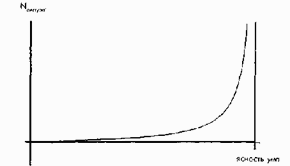
\includegraphics[scale=0.5]{figures/fig-1.png}

Ясность ума ($C_m$) зависит от множества переменных. Главную из них, сексуальный голод, можно обозначить как $sigma$, по очевидной анатомической аналогии, которую Уотерхауз на данной стадии своего эмоционального развития находит забавной.

Сексуальный голод начинается с нуля при $t = t_0$ (сразу после эякуляции) и растет как линейная функция времени

$$
\sigma \propto (t - t_0)
$$

Единственный способ снова свести его к нулю --- организовать новое семяизвержение.

Существует пороговое значения $sigma_c$, такое, что при $sigma > sigma_c$, Уотерхауз не способен ни на чем сосредоточиться, или, приблизительно

$$
C_m \propto \lim_{n \to \infty} \frac {1} {(\sigma - \sigma_c)^n}
$$


To есть, как только $sigma$ превышает пороговое значение $sigma_c$, Уотерхауз начисто утрачивает способность взламывать японские шифры. Это означает, что он не может достичь счастья (если, как сейчас, поблизости нет органа).

Обычно $sigma$ превышает $sigma_c$ через два три дня после семяизвержения:

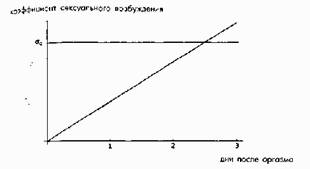
\includegraphics[scale=0.5]{figures/fig-2.png}

Значит, для поддержания душевного здоровья Уотерхаузу необходимо кончать каждые два три дня. Пока это удается, $sigma$ демонстрирует классическое пилообразное поведение, в идеале с пиками около $sigma_c$, закрашенные серым участки отмечают периоды, когда он абсолютно ничего не может сделать для победы над японским милитаризмом.

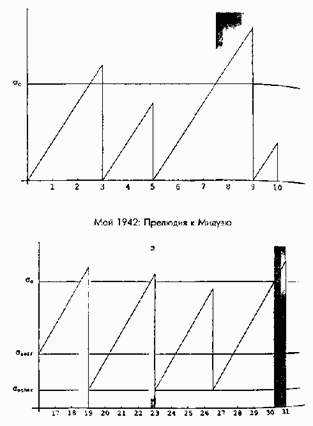
\includegraphics[scale=0.5]{figures/fig-3.png}

Вот и вся теоретическая основа. В Перл Харборе он обнаружил некоторую закономерность, которой поначалу не придал никакого значения. А именно, что семяизвержение в борделе (т.е. осуществленное с участием настоящей человеческой женщины) снижает уровень $sigma$ куда значительнее, чем то, которого Уотерхауз достигает, работая руками. Другими словами, уровень сексуального возбуждения после оргазма не всегда равен нулю, как постулировала изложенная выше наивная теория, но соответствует некой величине, зависящей от того, кончил он самостоятельно или с посторонней помощью: $sigma = sigma_{self}$ после мастурбации, но $sigma = sigma_{other}$ после публичного дома, причем $sigma_{self} > sigma_{other}$. Это неравенство во многом определило успехи Уотерхауза во взломе японских шифров на станции Гипо, где доступность большого количества публичных домов позволяла ему дольше держаться между оргазмами.

Обратите внимание на двенадцатидневный период 19-31 мая 1942 года с единственным перебоем в производительности. Можно утверждать, что в эти без малого две недели Уотерхауз единолично выиграл битву за Мидуэй.

Если бы он задумался об этом тогда, то обеспокоился, потому что из $sigma_{self} > sigma_{other}$ вытекают неприятные следствия, тем более что значение этих величин по отношению к $sigma_c$ непостоянно. Если бы не это неравенство, Уотерхауз мог бы функционировать как вполне самодостаточная и независимая единица. Однако $sigma_{self} > sigma_{other}$ подразумевает, что ясность его ума и, следовательно, его счастье зависят от других людей. Вот подлость!

Наверное, он потому и старался об этом не думать, что уходил от сложностей. Через неделю после встречи с Мэри Смит он понимает, что думать все таки придется.

Появление Мэри Смит загадочным образом сдвинуло всю систему уравнений. Теперь, когда он кончает, ясность ума не повышается скачкообразно, как ей положено. Он продолжает думать о Мэри. И как прикажете работать на победу?

Он отправляется на поиски борделя в надежде, что старая добрая $sigma_{other}$ его выручит. Здесь есть определенное затруднение. В Перл Харборе все было просто и ясно. Однако пансион миссис Мактиг расположен в добропорядочном районе; если здесь и есть бордели, это, во всяком случае, стараются скрыть. Так что Уотерхауз спешит в центр, что не просто в городе, где двигатели внутреннего сгорания работают на угле. Более того, миссис Мактиг за ним приглядывает. Она знает его привычки. Если он вернется с работы на четыре часа позже обычного или выйдет вечером, это придется объяснять. И объяснять убедительно, потому что миссис Мактиг взяла Мэри под свое дряблое крыло и способна нашептать ей всякие гадости. Хуже того, объясняться надо будет на людях, за столом, в присутствии кузена Мэри (которого, как выяснилось, зовут Род).

Но, черт возьми, Дулитл бомбил Токио, неужели Уотерхауз не сможет пробраться в бордель?! На подготовку уходит неделя (в течение которой он абсолютно не способен выполнять полезную работу из за непомерно возросшего уровня $sigma$). В итоге все трудности преодолены.

Становится полегче, но только на уровне сдерживания $sigma$. До недавнего времени больше ничего не требовалось бы. Однако теперь (как осознает Уотерхауз путем долгих раздумий в часы, когда должен был бы взламывать шифры) в системе уравнений, определяющих его поведение, появилась новая переменная; надо будет написать Алану, чтобы тот добавил команды в Уотерхауз моделирующую машину Тьюринга. Эта новая переменная --- FMSp, или фактор присутствия Мэри Смит.

В простой вселенной FMSp был бы ортогонален $sigma$, то есть эти две переменные абсолютно не зависели бы одна от другой. Уотерхауз кончал бы по графику, сдерживая уровень $sigma$. Одновременно он старался бы чаше общаться с Мэри Смит храняя FMSp на возможно более высоком уровне.

Увы! Вселенная не проста. FMSp и $sigma$ мало что не ортогональны, они переплетаются, как инверсионные следы самолетов в ближнем бою. Старая система сдерживания $sigma$ больше не работает, а платонические отношения не улучшают FMSp, а ухудшают. Его жизнь, до сих пор подчинявшаяся более или менее линейным зависимостям, превратилась в дифференциальное уравнение.

Он осознал это после визита в публичный дом. На флоте сходить к девочкам --- все равно что поссать в шпигат во время шторма; в худшем случае можно сказать, что при других обстоятельствах это было бы невоспитанно. Так что Уотерхауз ходил к девочкам много лет и ничуть не смущался.

Однако во время первого после знакомства с Мэри похода в публичный дом и после он себе отвратителен. Он видит себя не своими глазами, но глазами Мэри, и Рода, и миссис Мактиг и других приличных богобоязненных людей, на которых прежде чихать хотел.

Похоже, вторжение FMSp в уравнение его счастья --- только острие клина, и следом в жизнь Лоуренса Притчарда Уотерхауза ворвется еще больше неконтролируемых факторов, прежде всего необходимость общаться с нормальными людьми. Жуткое дело, но он понимает, что готов пойти на танцы.

Танцы устраивает Австралийское добровольческое общество --- подробностей Уотерхауз не знает и знать не хочет. Миссис Мактиг, очевидно, считает, что за плату, которую взимает с жильцов, обязана не только кормить поить их, но и женить, поэтому настойчиво уговаривает ходить на танцы и приглашать девушек. Наконец Род, чтобы отвязаться, говорит, что придет с большой компанией, в которой будет и его кузина Мэри. Род под два с половиной метра, его несложно будет найти в толпе. Если повезет, миниатюрная Мэри окажется где то рядом.

Так что Уотерхауз идет на танцы, лихорадочно подыскивая слова, с которыми обратится к Мэри. В голову приходят несколько вариантов.

<<Знаете ли вы, что японская промышленность способна выпускать лишь сорок бульдозеров в год?>> Тогда следующая фраза. <<Неудивительно, что на земляных работах они вынуждены использовать рабов>>.

Или: <<В силу конструктивных ограничений, накладываемых конфигурацией антенны, у японских флотских радарных систем есть сзади слепое пятно --- к ним желательно приближаться точно с кормы>>.

Или: <<Шифры, которыми пользуются низовые подразделения японской армии, на самом деле труднее взломать, чем шифры командования. Ну разве не забавно?>>

Или: <<Так вы родом из деревни... вы делаете домашние заготовки? Вам, наверное, интересно будет узнать, что близкие родственники бактерий, из за которых вздуваются консервы, вызывают газовую гангрену>>.

Или: <<Японские линкоры начали самопроизвольно взрываться, потому что высокоэксплозивные материалы в погребе боеприпасов становятся химически неустойчивы>>.

Или: <<Доктор Алан Тьюринг из Кембриджа утверждает, что душа --- это выдумка, и все, определяющее нас как людей, можно свести к ряду механических операций>>.

И так далее в том же духе. Пока он не нашел ничего такого, чтобы гарантированно сразило бы Мэри наповал. Более того, у него нет ни малейшего представления, как себя вести. У него всегда так было с женщинами, вот почему он ни разу не завел девушки.

Но сегодня все иначе. Это жест отчаяния.

Что сказать про танцы? Большое помещение. Мужчины в форме и по большей части выглядят незаслуженно хорошо. Много лучше, чем Уотерхауз. Женщины в платьях и с прическами. Губная помада, жемчуг, биг бэнд, белые перчатки, мордобой, кто то исподтишка целуется, кто то украдкой блюет. Уотерхауз опаздывает --- снова проблема транспортировки. Весь бензин ушел на то, чтобы большие бомбардировщики осыпали японцев взрывчатыми веществами. Перевезти комок плоти по фамилии Уотерхауз через Брисбен, чтобы он попытался лишить невинности девушку, --- последняя задача в списке. Ему приходится долго идти в жестких кожаных ботинках, которые по пути несколько утрачивают свой блеск. К концу дороги он окончательно убежден, что они годятся единственно для остановки артериального кровотечения из ран, ими же причиненных.

Ближе к концу вечера он замечает Рода. После нескольких танцев (поскольку у того нет отбоя от партнерш) Род наконец направляется в угол, где все друг друга знают, все веселятся и вообще прекрасно обходятся без Уотерхауза.

Наконец он различает шею Мэри Смит, которая сквозь тридцать ярдов густого табачного дыма выглядит такой же невыразимо желанной, что и в гостиной миссис Мактиг. Уотерхауз берет курс на нее, как морской пехотинец --- на японский дот, перед которым и сложит голову. Интересно, награждают посмертно геройски павших на танцах?

Он все еще в нескольких шагах, бредет, как в угаре, к белой колонне шеи, когда внезапно музыка стихает и до слуха доносятся голоса Мэри и ее друзей. Они весело болтают, но не пo aнглийски.

Наконец Уотерхауз разбирает выговор. Более того, он разгадывает загадку писем, приходивших в пансион миссис Мактиг адресованных кому то по фамилии сСмндд.

Все ясно! Мэри и Род --- йглмиане. И фамилия их не Смит --- просто звучит похоже на Смит. Их фамилия --- сСмндд. Род вырос в Манчестере --- вероятно, в каком то йглмском гетто, --- Мэри происходит из той ветки семьи, которую пару поколений назад выслали в Большую Песчаную Пустыню за нелады с законом (надо думать, мятеж).

Вот пусть Тьюринг такое объяснит. Поскольку это доказывает, что есть Бог и, более того, что Он --- личный друг и помощник Лоуренса Притчарда Уотерхауза. Вопрос первой фразы решен идеально, как теорема. Q.E.D., крошка. Уотерхауз уверенно шагает вперед, жертвуя хищным ботинкам еще квадратный сантиметр кожи. Как удастся восстановить много позже, при этом он встает между Мэри и парнем, с которым та пришла на танцы, и, может быть, толкает того под локоть, так что парень проливает пиво. Все смолкают. Уотерхауз открывает рот и произносит:

--- Гкснн бхлдх сйрд м!

--- Эй, приятель! --- говорит парень, с которым Мэри пришла на танцы.

Уотерхауз поворачивается на голос. Дурацкая ухмылка на его лице представляет собой вполне подходящую мишень, и парень безошибочно попадает в нее кулаком. У Лоуренса мгновенно немеет нижняя часть головы, рот наполняется теплой, питательной на вкус жидкостью. Бетонный пол взлетает, крутясь, как подброшенная монета, и отскакивает от его виска. Все четыре конечности Уотерхауза прижаты к полу весом его торса.

Какое то оживление происходит в далекой плоскости человеческих голов, на высоте пяти шести футов от пола, где обычно и протекает нормальное общение. Парня, который стоял с Мэри, оттаскивает в сторону кто то сильный --- под таким углом трудно различать лица, но вполне вероятно, что это Род. Он кричит на йглмском. Вообще все кричат на йглмском, даже те, кто говорит по английски, потому что у Лоуренса травматическое расстройство центров распознавания речи. Лучше оставить все эти изыски на потом и заняться более насущным филогенезом: например, замечательно было бы снова стать позвоночным. После этого, возможно, удастся в отдаленной перспективе перейти к прямохождению.

Тощий йглмско австралийский парень в форме военного летчика подходит и тянет его за правый передний плавник, рывком втаскивая Уотерхауза по эволюционной лестнице --- не для того чтобы помочь, но чтобы получше разглядеть лицо. Летчик кричит (потому что музыка заиграла снова):

--- Где ты научился так говорить?

Уотерхауз не знает, с чего начать: упаси Бог снова обидеть этих людей. Однако слов и не требуется. Летчик кривится от омерзения, как будто у Лоуренса из глотки лезет двухметровый солитер.

--- На Внешнем Иглме? --- спрашивает он.

Уотерхауз кивает. Изумленные и потрясенные лица застывают каменными масками. Ну конечно! Они с Внутреннего Йглма! Жителей этого острова постоянно притесняют; у них и музыка самая лучшая, и люди самые интересные, однако их постоянно шлют на Барбадос рубить сахарный тростник, или в Тасманию гонять овец, или... ну, скажем, в юго восточную часть Тихого океана, бегать по джунглям от обвешанных взрывчаткой голодных камикадзе.

Летчик выдавливает улыбку и легонько хлопает Уотерхауза по плечу. Кто то из присутствующих должен взять на себя неприятную дипломатическую работу и сгладить инцидент. Летчик, с истинным внутренне йглмским тактом, взял это на себя.

--- У нас, --- бодро объясняет он, --- так говорить невежливо.

--- Да? --- недоумевает Уотерхауз. --- А что я такого сказал?

--- Ты сказал, что был на мельнице, чтобы заявить протест по поводу лопнувшего во вторник мешка, и по тону, которым разговаривал мельник, смог заключить, что незамужняя двоюродная бабушка Мэри, пользовавшаяся в юности довольно сомнительной репутацией, подцепила грибок на ногтях.

Долгое молчание. Потом все начинают говорить разом. Наконец сквозь какофонию прорывается женский голос:

--- Нет! Нет!

Уотерхауз смотрит в ту сторону: это Мэри.

--- Я так поняла, что он вошел в пивную, где хотел предложить себя в качестве крысоморильщика, и что у собаки моей соседки --- водобоязнь.

--- Он был в исповедальне... священник... грудная жаба... --- кричит кто то из за ее спины.

Потом все снова говорят разом:

--- Пристань... молочная сестра Мэри... проказа... жаловал на шумное сборище!

Сильная рука обнимает Уотерхауза за плечи и разворачивает от спорящих. Обернуться и посмотреть, кто его держит, Лоуренс не может, потому что позвонки снова сместились. Надо думать, это Род благородно взял под свое крыло недотепу янки. Род вынимает из кармана носовой платок, прикладывает Уотерхаузу к лицу и убирает руку. Платок остается висеть на губе, которая формой сейчас напоминает аэростат заграждения.

Этим доброта Рода не ограничивается. Он приносит Уотерхаузу выпить и находит ему стул.

--- Слыхал про навахо? --- спрашивает Род.

--- А?

--- Ваша морская пехота использует в качестве радистов индейцев навахо --- они говорят по рации на своем языке и нипы ни хера не понимают.

--- А. Да, --- говорит Уотерхауз.

--- Уинни Черчиллю глянулась эта идейка. Решил, что вооруженным силам Его Величества тоже такое нужно. Навахо у нас нет. Но...

--- У вас есть йглмцы, --- понимает Уотерхауз.

--- Действуют две программы, --- говорит Род. --- На флоте используют внешних йглмцев. В армии и ВВС --- внутренних.

--- И как?

--- Более или менее. Йглмский язык очень емкий. Ничего общего с английским или кельтским. Ближайшие родственные языки --- йнд, на котором говорит одно племя мадагаскарских пигмеев, и алеутский. Но ведь чем емче, тем лучше, верно?

--- Несомненно, --- соглашается Уотерхауз. --- Меньше избыточность, труднее взломать шифр.

--- Проблема в том, что язык этот если не совсем мертвый, то уж точно лежит на смертном одре. Понятно?

Уотерхауз кивает.

--- Поэтому каждый слышит немного по своему. Как сейчас. Они услышали твой внешнейглмский акцент и заподозрили оскорбление. Я то отлично все понял: во вторник ты был на мясном рынке и слышал, будто Мэри быстро идет на поправку и вскоре совсем станет на ноги.

--- Я хотел сказать, что она прекрасно выглядит! --- возмущается Уотерхауз.

--- А! --- говорит Род. --- Тогда тебе надо было сказать: <<Гкснн бхлдх сйрд м!>>

--- Но я это и сказал!

--- Ты спутал среднегортанный с переднегортанным, --- разъясняет Род.

--- Только честно, --- просит Уотерхауз, --- можно ли их различить по трескучей рации?

--- Нет, --- признается Род. --- По рации мы говорим только самое основное: <<Двигай туда и захвати этот дот, не то я тебе яйца оторву>>, и все такое.

Вскоре оркестр заканчивает играть. Народ расходится.

--- Послушай, --- просит Уотерхауз. --- Может, передашь Мэри, что я на самом деле хотел сказать?

--- Не нужно, --- убежденно говорит Род. --- Мэри прекрасно разбирается в людях. Мы, йглмцы, очень сильны в невербальном общении.

Уотерхауз с трудом сдерживает ответ <<Немудрено>>, за который, вероятно, снова схлопотал бы по морде. Род пожимает ему руку и уходит. Уотерхауз, блокированный ботинками, ковыляет вслед.


\chapter{I.N.R.I}


Гото Денго шесть недель лежит на тростниковой койке. Белую москитную сетку над ним колышет ветерок из окна. Во время тайфуна сестры закрывают окно перламутровыми ставнями, но обычно оно распахнуто и днем, и ночью. За окном --- склон, превращенный трудами поколений в исполинскую лестницу. Когда встает солнце, рисовые всходы на террасах флюоресцируют; зеленый свет заливает комнату, как отблески пламени. Скрюченные людишки в яркой одежде пересаживают рисовые ростки и возятся с оросительной системой. Стены в палате белые, оштукатуренные, трещинки ветвятся на них, как кровеносные сосуды в глазу. Единственное украшение --- резное деревянное распятие, выполненное в маниакальных подробностях, глазные яблоки у Христа --- гладкие, без зрачка и радужки, как у римских статуй. Он кособоко обвис на кресте, руки раскинуты, связки, вероятно, порваны, ноги, перебитые древком римского копья, не в силах поддерживать тело. Каждая ладонь пробита корявым ржавым гвоздем; на ноги хватило одного. Через некоторое время Гото Денго замечает, что скульптор расположил все три гвоздя в вершинах идеального правильного треугольника. Они с Иисусом много часов и дней, не отрываясь, пялятся друг на друга сквозь белый марлевый полог; когда ветер колышет ткань, кажется, что Иисус корчится. Над распятием укреплен развернутый свиток, на нем надпись: <<I.N.R.I.>>. Гото Денго мучительно пытается разгадать аббревиатуру, но в голову лезет какая то ерунда.

Занавеска расходится. Над койкой стоит идеальная девушка в строгом черно белом одеянии, осиянная зеленым светом рисовых всходов. Она снимает с Гото Денго больничный халат и начинает тереть его губкой. Гото Денго указывает на распятие и задает вопрос. Может быть, девушка немного знает японский. Если она и слышит, то не подает виду. Наверное, глухая, или дурочка, или то и другое вместе --- христиане обожают убогих. Сосредоточив взгляд на его теле, она трет нежно, но неумолимо один квадратный сантиметр за другим. Сознание по прежнему временами шутит с ним шутки; когда Гото Денго смотрит на собственный голый торс, все на мгновение переворачивается: ему чудится, будто он смотрит на пригвожденного Христа. Ребра выпирают, кожа --- сплошные рубцы и болячки. Он явно больше ни на что не годен; почему его не отправили в Японию? Почему просто не убили? <<Вы говорите по английски?>> --- спрашивает Гото Денго. Большие карие глаза стремительно расширяются. Девушка несравненно хороша --- красивее всех, кого он видел в своей жизни. Наверное, Гото ей омерзителен --- препарат под микроскопом в прозекторской. Наверное, выйдя из палаты, она будет долго мыться, а потом постарается каким нибудь занятием изгнать воспоминание о его теле из своего чистого, целомудренного ума.

Он проваливается в забытье и видит себя глазами москита, лезущего сквозь марлю: искалеченное, распластанное на деревяшке тело, словно прихлопнутый комар. Узнать в нем японца можно лишь по белой полоске ткани на лбу, но вместо оранжевого солнца на ней надпись: <<I.N.R.I.>>.

Рядом с кроватью сидит мужчина в черной рясе, перебирает красные коралловые четки с маленьким распятием. У него большая голова и выпуклый лоб, как у тех странных людей, которые копошатся на рисовых полях, однако высокие залысины и каштановые с проседью волосы --- явно европейские, и внимательные глаза --- тоже.

--- Iesus Nasarenus Rex Iudaeorum, --- говорит он. --- Это латынь. Иисус Назорей Царь Иудейский.

--- Иудейский? Я думал, Иисус был христианин, --- говорит Гото Денго.

Человек в черной рясе смотрит на него, не отвечая. Гото Денго делает новый заход:

--- Я не знал, что евреи говорят на латыни.

Однажды в комнату ввозят кресло каталку; Гото Денго таращится в тупом изумлении. Он слыхал про такие: на них за высокими стенами, вдали от посторонних глаз, возят из комнаты в комнату постыдно неполноценных людей. И вдруг хрупкие девушки хватают его и сажают в кресло! Они что то говорят про свежий воздух; в следующий миг Гото Денго выкатывают из палаты и везут по коридору! Его привязали, чтобы не вывалился; он смущенно ерзает, пытаясь спрятать лицо. Девушки выкатывают кресло на большую веранду с видом на гору. От листьев поднимается пар, кричат птицы. На стене за спиной --- огромная картина: привязанный к столбу голый I.N.R.I. исполосован сотнями параллельных кровавых следов. Рядом центурион с бичом. Глаза у центуриона странно японские.

На веранде еще три японца в инвалидных креслах. Один невнятно разговаривает сам с собой и все время теребит болячку на руке, так что кровь капает на подстеленное полотенце. У другого обгорели руки и лицо, он смотрит на мир через единственную дырку в черном коллоидном рубце. Третьего накрепко прибинтовали к креслу, потому что он все время бьется, как рыба на песке, и бессвязно вскрикивает.

Гото Денго смотрит на перила веранды, прикидывая, хватит ли сил подъехать к ним и перекинуться через парапет. Почему ему не дали умереть с честью?

Команда подводной лодки обходилась с ним и другими эвакуированными непонятно: почтительно и в то же время гадливо.

Когда он стал изгоем? Явно задолго до эвакуации с Новой Гвинеи. Лейтенант, спасший его от охотников за головами, обходился с ним как с предателем. Но он и раньше был не таким, как все. Почему его не съели акулы? Может, его мясо пахло иначе? Он должен был погибнуть вместе с товарищами в море Бисмарка. Его спасло отчасти везение, отчасти умение плавать.

Почему он умеет плавать? Отчасти потому, что отец учил его не верить в демонов.

Он громко смеется. Другие японцы оборачиваются.

Его учили не верить в демонов, теперь он сам --- демон.

В следующий приход чернорясый громко смеется над Гото Денго.

--- Я не пытаюсь вас обратить, --- уверяет он. --- Пожалуйста не говорите об этом старшим. Заниматься прозелитизмом строго запрещено, и нас жестоко накажут.

--- Вы пытаетесь обратить меня не словами, а тем, что держите здесь, --- говорит Гото Денго. Ему не хватает английского.

Чернорясого зовут отец Фердинанд. Он иезуит или что то вроде того; владение английским дает ему неограниченную свободу маневра.

--- Каким образом мы обращаем вас в свою веру, всего лишь приняв сюда? --- Потом, чтобы окончательно выбить у Гото Денго землю из под ног, повторяет то же самое на более или менее сносном японском.

--- Не знаю. Живопись. Скульптура.

--- Если вам не нравится наша живопись, закройте глаза и думайте об императоре.

--- Я не могу все время держать глаза закрытыми.

Отец Фердинанд фальшиво смеется.

--- Почему? Большинство ваших соотечественников успешно живет с закрытыми глазами от колыбели до могилы.

--- Почему бы вам не повесить что нибудь повеселее? Это больница или морг?

--- La Pasyon очень важна здесь, --- говорит отец Фердинанд.

--- La Pasyon?

--- Страдания Христа. Они очень понятны филиппинскому народу. Особенно сейчас.

У Гото Денго есть еще одна жалоба, но, чтобы ее высказать, приходится одолжить у отца Фердинанда японо английский словарь и поработать несколько дней.

--- Правильно ли я понял? --- говорит отец Фердинанд. --- Вы считаете, что, окружив заботой и милосердием, мы тем самым исподволь пытаемся обратить вас в католичество?

--- Вы извращаете мои слова, --- говорит Гото Денго.

--- Я их выправляю, --- парирует отец Фердинанд.

--- Вы пытаетесь сделать меня одним из вас.

--- Одним из нас? В каком смысле?

--- Презренной личностью.

--- Зачем нам это?

--- Потому что у вас жалкая религия. Религия побежденных. Если вы сделаете меня жалкой личностью, мне захочется принять вашу религию.

--- Обходясь с вами достойно, мы пытаемся сделать вас жалкой личностью?

--- В Японии с больным не обходились бы так хорошо.

--- Можете не объяснять, --- говорит отец Фердинанд. --- Вы в стране, где многих женщин изнасиловали японские военные.

Пора менять тему.

--- Ignoti et quasi occulti --- Societas Eruditorum, --- говорит Гото Денго, читая надпись на медальоне, который висит у отца Фердинанда на груди. --- Опять латынь? Что это значит?

--- Это организация, к которой я принадлежу. Она межконфессиональная.

--- Что это значит?

--- Любой может в нее вступить. Даже вы, когда поправитесь.

--- Я поправлюсь, --- говорит Гото Денго. --- Никто не будет знать, что я болел.

--- Кроме нас. Ах да, понял. Никто из японцев не узнает. Да, правда.

--- Но другие не поправятся.

--- Тоже правда. Из всех здешних пациентов у вас самый лучший прогноз.

--- Вы взяли больных японцев на свое попечение...

--- Да. Этого более или менее требует наша религия.

--- Теперь они жалкие личности. Вы хотите, чтобы они приняли вашу жалкую религию.

--- Только в той мере, насколько им это на благо, --- говорит отец Фердинанд. --- Не потому, что они побегут и построят нам новый собор.

На следующий день Гото Денго выписывают. Он не чувствует себя здоровым, однако готов на все, лишь бы выбраться из этой колеи --- день за днем играть в гляделки с Царем Иудейским.

Он думает, что его нагрузят вещмешком и отправят на автобусную остановку --- добирайся, как знаешь. Тем не менее за ним приезжает автомобиль. Мало того, автомобиль подруливает к лётному полю, где Гото Денго сажают на маленький самолет. Он впервые летит по воздуху: волнение живительнее, чем полтора месяца в больнице. Самолет пролетает между двумя зелеными горами и (судя по солнцу) берет курс на юг. Только сейчас Гото Денго понимает, где был: в центре острова Лусон, к северу от Манилы.

Через полчаса они над столицей; внизу река Пасиг, потом залив, сплошь забитый транспортными судами. Подступы к морю охраняет пикет кокосовых пальм. Когда смотришь сверху, кажется, что ветки корчатся на ветру, словно насаженные на шип исполинские тарантулы. Гото Денго заглядывает пилоту через плечо и видит к югу от города две пересекающиеся под острым углом взлетно посадочные полосы. Самолет начинает <<козлить>> от порывов ветра. Он подпрыгивает на полосе, словно передутый футбольный мяч, проносится мимо большей части ангаров и тормозит у отдельно стоящей караулки. Рядом дожидается человек на мотоцикле с коляской. Гото Денго жестами велят идти к мотоциклу; никто с ним не разговаривает. На нем армейская форма без знаков отличия.

На сиденье лежат мотоциклетные очки; Гото Денго надевает их, чтобы защитить глаза от насекомых. Немного страшно, потому что у него нет ни удостоверения, ни приказов. Однако с авиа базы их выпускают без всякой проверки документов.

Мотоциклист --- молодой филиппинец --- все время широко улыбается, не боясь, что насекомые застрянут в больших белых зубах. Он явно убежден, что у него лучшая работа в мире; может быть, так и есть. Он сворачивает на южную дорогу, которая, наверное, считается в здешних краях крупной магистралью, и начинает лавировать в потоке транспорта. В основном это повозки запряженные индийскими буйволами --- огромными, с внушительными серповидными рогами. Автомобилей мало, изредка попадаются армейские грузовики.

Первые часа два дорога идет прямо, через плоскую сырую местность, где прежде выращивали рис. Гото Денго замечает слева водное пространство, но не знает, часть это океана или большое озеро.

--- Лагуна де Бай, --- говорит мотоциклист, проследив его взгляд. --- Очень красиво.

Потом они сворачивают от лагуны на дорогу, что поднимается к плантациям сахарного тростника. Внезапно Гото Денго замечает вулкан: черный от растительности конус окутан туманом, словно москитной сеткой. Воздух такой плотный, что невозможно оценить размер и расстояние --- то ли это шлаковый конус у самой дороги, то ли огромный стратовулкан в пятидесяти милях дальше.

Бананы, кокосовые пальмы, масличные и финиковые пальмы, поначалу редкие, преображают местность в своего рода влажную саванну. Мотоциклист заходит в придорожную лавчонку купить бензин. Гото Денго вытаскивает растрясенное тело из коляски и садится за столик под зонтиком. Достает из кармана чистый носовой платок, который нашел там сегодня утром, вытирает со лба пыль и капельки пота, потом заказывает питье. Ему приносят стакан ледяной воды, миску неочищенного местного сахара и тарелку лаймов каламанси размером с фасолину. Он выжимает лаймы в воду, размешивает сахар и жадно пьет.

Мотоциклист подсаживается за столик и убалтывает хозяина на стакан бесплатной воды. С его лица не сходит проказливая улыбка, как будто у них с Гото Денго какой то общий секрет. Он подносит к плечу воображаемое ружье.

--- Ты солдат?

Гото Денго задумывается.

--- Нет. Я недостоин зваться солдатом.

Мотоциклист изумляется.

--- Не солдат? Я думал, ты солдат. А кто ты?

Гото Денго хочет ответить, что он поэт. Но и это для него слишком высокое звание.

--- Я --- горняк, --- говорит он наконец. --- Копаю землю.

--- А а а... --- тянет мотоциклист, как будто понял. --- Хочешь?

Он вынимает из кармана две сигареты.

Уловка настолько изящная, что Гото Денго смеется.

--- Эй! --- говорит он хозяину. --- Сигареты!

Водитель ухмыляется и прячет свои сигареты назад в карман. Хозяин подходит и протягивает Гото Денго пачку <<Лаки Страйк>> и коробок спичек.

--- Сколько? --- Гото Денго вынимает конверт с деньгами, которые утром нашел у себя в кармане. Вытаскивает купюры: на каждой по английски написано <<ЯПОНСКОЕ ПРАВИТЕЛЬСТВО>> и достоинство в песо. Посредине изображение обелиска, памятнику Хосе П. Рисалю перед гостиницей <<Манила>>.

Хозяин морщится.

--- Серебро есть?

--- Серебро? Металл?

--- Да, --- говорит мотоциклист.

--- Тут им расплачиваются?

Водитель кивает.

--- А это не годится? --- Гото Денго протягивает новенькие, хрустящие банкноты.

Хозяин берет конверт, отсчитывает несколько самых крупных купюр, сует их в карман и уходит.

Гото Денго срывает наклейку, постукивает пачкой по столу и распечатывает ее. Кроме сигарет, в ней карточка. Видна только верхняя часть: карандашный профиль мужчины в офицерской фуражке. Гото Денго медленно вытягивает карточку и видит сначала орла на фуражке, потом лётные очки, огромную трубку, лацкан с четырьмя звездами и, наконец, надпись печатными буквами <<Я ВЕРНУСЬ>>.

Мотоциклист старательно разыгрывает беспечность. Гото Денго показывает ему карточку и поднимает брови.

--- Глупости, --- говорит мотоциклист. --- Япония очень сильная. Японцы будут здесь всегда. Макартур умеет только продавать сигареты.

В спичечном коробке лежит такой же портрет Макартура с теми же словами на обороте.

Покурив, они едут дальше. Теперь уже повсюду --- слепленные черные конусы вулканов, дорога ныряет то вверх, то вниз. Деревья подступают ближе и ближе, и вот они уже едут через своего рода культурные джунгли: ананасы внизу, кусты кофе и какао посередине, бананы и кокосовые пальмы наверху. Одна деревушка сменяется другой --- покосившиеся лачуги жмутся к приземистой и крепкой, на случай землетрясения, большой белой церкви. У обочин свалены в кучу кокосовые орехи; они рассыпаются на дорогу, их приходится объезжать. Наконец мотоцикл сворачивает с основной дороги на проселочную, вьющуюся среди деревьев. Колеи разъезжены шинами грузовиков, слишком широких для проселка; земля усыпана недавно сбитыми ветками.

Им попадается брошенная деревня. Двери болтаются на петлях, по лачугам шастают бродячие псы. Над грудой зеленых кокосовых орехов роятся черные мухи.

Еще через милю культурный лес сменяется диким. Дорогу преграждает КПП. Водитель больше не улыбается.

Гото Денго называет часовому свою фамилию. Он не знает цели приезда, поэтому ничего больше сказать не может. Наверное, здесь концлагерь, куда его заключат. Присмотревшись, он видит натянутую между деревьями колючую проволоку и второе ограждение внутри первого. Видно, где вырыты бункеры и устроены доты; можно определить сектора обстрела. С верхушек самых высоких деревьев свешиваются веревки, чтобы снайперы могли при необходимости привязать себя к веткам. Все по науке, но на войне такого совершенства не бывает, только в учебке.

Постепенно до него доходит, что цель укреплений --- не удержать людей внутри, а не допустить их снаружи.

Происходит телефонный разговор, барьер поднимают и машут: проезжайте. Примерно через милю они видят расчищенный кусок джунглей; на платформах из свежесрубленных стволов поставлены палатки. В тени дожидается лейтенант.

--- Здравствуйте, лейтенант Гото. Я --- лейтенант Мори.

--- Вы недавно прибыли в Южную Сырьевую Зону, лейтенант Мори?

--- Да. Как вы догадались?

--- Вы стоите под кокосовой пальмой.

Лейтенант Мори поднимает голову и видит прямо над собой несколько коричневых волосатых ядер.

--- Ах, вот как! --- Он отходит от дерева. --- Вы разговаривали с мотоциклистом по пути сюда?

--- Мы перекинулись парой слов.

--- О чем вы говорили?

--- Сигареты. Серебро.

--- Серебро? --- Лейтенант очень заинтересован, и Гото Денго вынужден повторить весь разговор.

--- Вы говорили ему, что были горняком?

--- Да, что то в таком роде.

Лейтенант Мори отступает на шаг и кивает стоящему в сторонке рядовому. Тот отрывает приклад от земли, берет ружье наперевес и поворачивается к мотоциклисту. За шесть шагов он успевает набрать разгон и с гортанным криком вонзает штык в тощий живот филиппинца. Тот отрывается от земли и, ахнув, падает навзничь. Солдат, расставив ноги, встает над ним и еще несколько раз с влажным скрипом вгоняет штык в грудь.

Наконец тот застывает неподвижно, кровь хлещет из него во все стороны.

--- Ваша неосторожность не будет поставлена вам в вину, --- бодро говорит лейтенант Мори, --- поскольку вы не знали, в чем состоит ваше новое задание.

--- Простите?

--- Горное дело. Вы будете заниматься горным делом, Гото сан. --- Лейтенант замирает по стойке <<смирно>> и низко кланяется. --- Позвольте мне первым вас поздравить. У вас очень важное задание.

Гото Денго возвращает поклон, не зная точно, как низко надо кланяться.

--- Так я не... --- Он судорожно ищет слова. Пария? Изгой? Приговоренный к смерти? --- Я не жалкая личность?

--- Вы здесь очень уважаемая личность, Гото сан. Прошу следовать за мной. --- Лейтенант Мори указывает на одну из палаток.

Идя прочь, Гото Денго слышит, как молодой мотоциклист бормочет какие то слова.

--- Что он сказал? --- спрашивает лейтенант Мори.

--- Он сказал: <<Отче, в руки твои предаю дух мой>>. Это религиозное, --- объясняет Гото Денго.


\chapter{КАЛИФОРНИЯ}


Такое впечатление, что половина персонала в Международном аэропорту Сан Франциско --- филиппинцы, Что безусловно, смягчает шок от возвращения в Америку. Таможенники --- стопроцентные англосаксы, --- как всегда, выбирают Рэнди для тщательного досмотра. Люди, путешествующие в одиночку и налегке, вызывают у американских представителей власти сильнейшую идиосинкразию. Они вовсе не считают тебя наркокурьером, просто ты подпадаешь под тип наиболее кретинически оптимистичного наркокурьера и прямо таки требуешь тебя обыскать. Досадуя, что ты их на это толкнул, они решают преподать наглядный урок: следующий раз, приятель, лети с женой и четырьмя детьми или с четырьмя огромными саквояжами на колесиках. И вообще думай головой! Не важно, что Рэнди прилетел из страны, где таблички <<СМЕРТЬ НАРКОТОРГОВЦАМ>> натыканы по всему аэропорту, как здесь <<ОСТОРОЖНО МОКРЫЙ ПОЛ>>.

Самый кафкианский момент --- когда таможенница спрашивает его о роде занятий, и надо придумать ответ, не похожий на судорожную ложь наркоторговца, чей живот распирают начиненные героином презервативы. <<Я работаю на частного телекоммуникационного провайдера>> по идее звучит достаточно невинно. <<А, вроде телефонной компании?>> --- недоверчиво переспрашивает таможенница. <<Телефонный рынок не настолько для нас доступен, --- говорит Рэнди, --- поэтому мы поставляем другие коммуникационные услуги. По большей части информацию>>. <<И для этого требуются частые разъезды ?>> --- спрашивает таможенница, листая последние, сплошь в пестрых штампах, странички его паспорта. Она выразительно смотрит на старшего таможенника. Тот подходит и встает рядом. Рэнди не по себе, в точности как начинающему наркокурьеру; он перебарывает желание вытереть потные ладони о штаны, после чего его бы наверняка прогнали через магнитный туннель контрольного компьютерного устройства, накормили тройной дозой слабительного и заставили три часа тужиться над горшком для вещдоков.

--- Да, --- говорит Рэнди.

Старший таможенник (настолько между прочим и ненавязчиво, что Рэнди с трудом подавляет хриплый смешок) начинает листать кошмарный журнал по телекоммуникации, который Рэнди сунул в сумку перед вылетом из Манилы. Слово ИНТЕРНЕТ встречается на обложке как минимум пять раз. Рэнди смотрит прямо в глаза таможеннице и говорит: <<Интернет>>. На ее лице проступает абсолютно фальшивое понимание. Она стреляет глазами в шефа. Тот, не отрываясь от статьи про высокоскоростные маршрутизаторы нового поколения, оттопыривает нижнюю губу и важно кивает. Как любой американец девяностых, он знает, что знакомство с подобными вещами --- такой же непременный атрибут мужчины, каким было для его отца умение заменить колесо. <<Я слышала, это страшно интересно>>, --- говорит таможенница совершенно иным тоном и начинает складывать вещи Рэнди в одну кучку, чтобы он мог убрать их назад в сумку. Все замечательно. Рэнди снова добропорядочный американский гражданин, которого власти ритуально постращали. У него острое желание махнуть в ближайший оружейный магазин и оставить там примерно десять тысяч долларов. Не то чтобы он хотел кого нибудь убить, просто от общения с официальными лицами его трясет. Наверное, он чересчур много времени провел с Томом Говардом, коллекционером оружия и стрелком любителем. Сперва агрессия по отношению к тропическим лесам, теперь желание приобрести автомат. Куда он катится?

Высокая бледная фигура Ави маячит за бархатной веревкой, вокруг охваченные неистовством филиппинки потрясают гладиолусами, как боевым копьями. Ави засунул руки в карманы метущего по полу пальто; голова повернута в сторону Рэнди, но взгляд застыл на точке где то посередине между ними, брови сосредоточенно сведены. Также хмурилась бабушка Рэнди, распутывая моток бечевки из ящика со всякой всячиной. У Ави такое выражение бывает, когда он делает нечто похожее с новым клубком информации. Наверное, прочел про золото. Рэнди упустил возможность классного розыгрыша: надо было положить в сумку пару свинцовых брусков и дать ее Ави --- вот бы тот офигел. Поздно. В тот миг, когда Рэнди подходит, Ави трогается с места. Несформулированный протокол предписывает, когда они должны жать друг другу руки, когда обниматься, а когда вести себя так, будто расстались пять минут назад. Недавний обмен электронной почтой, вероятно, знаменовал собой виртуальную встречу, отменив потребность в рукопожатиях и объятиях.

--- Ты был прав насчет сочных диалогов, --- первые слова Ави. --- Ты слишком много времени провел с Шафто и смотришь на вещи его глазами. Неправда, будто тебе что то хотели этим сказать. Вернее, хотели, но не то, что думает Шафто.

--- А какое твое объяснение?

--- Как тебе нравится мысль учредить новую валюту? --- Спрашивает Ави.

Рэнди часто ловил в аэропортах обрывки деловых разговоров: как прошла большая презентация, кто вероятный кандидат на вакантную руководящую должность и все такое. Он гордится, что они с Ави говорят о более возвышенных или по крайней мере более неординарных материях. Они идут через здание аэропорта. Из ресторанчика пахнет имбирем и соевым соусом; Рэнди на мгновение теряет ориентировку --- в каком он полушарии?

--- Хм, я как то не очень задумался, --- говорит он. --- Это что наш следующий этап? Учреждаем новую валюту?

--- Ну, очевидно, кто то должен учредить валюту, которая не будет полным говном.

--- Это что, юмор? --- спрашивает Рэнди.

--- Ты газеты читаешь? --- Ави хватает его за локоть и тащит к газетной стойке. Шапки некоторых газет посвящены валютному кризису в Юго Восточной Азии.

--- Я знаю, что валютные колебания имеют для <<Эпифита>> большое значение, --- говорит Рэнди, --- но это такая нудятина, что выть хочется.

--- Это не нудятина для нее. --- Ави хватает три разные газеты, напечатавшие одну и ту же фотографию, присланную телеграфным агентством: хорошенькая тайка в километровой очереди к банку держит одну единственную американскую долларовую бумажку.

--- Знаю, это серьезно для части наших клиентов, --- говорит Рэнди, --- просто не думал об этом как о деловой возможности.

--- А ты подумай. --- Ави вынимает несколько таких же, как у тайки, долларовых бумажек, расплачивается за газеты и поворачивается к выходу. Они попадают в туннель, ведущий к многоэтажной автомобильной парковке.

--- Султан считает...

--- Ты часто болтаешь с султаном?

--- Больше с Прагасу. Дашь мне закончить? Мы решили основать Крипту, верно?

--- Верно.

--- Что такое Крипта? Ты помнишь, как первоначально формулировалось ее назначение?

--- Надежное, анонимное, нерегулируемое хранилище данных. Информационный рай.

--- Ага. Свалка битов. И мы предполагали для нее различные применения.

--- Слушай, ведь правда! --- Рэнди вспоминает долгие ночи за кухонным столом или в гостиничном номере, когда они писали версии бизнес плана, теперь древние и забытые, как собственноручные подлинники Евангелий.

--- В том числе электронные банковские услуги. Черт, мы даже предвидели, что это будет одна из главных функций. Но когда бизнес план впервые входит в соприкосновение с настоящим рынком --- с реальным миром, --- все разом проясняется. Ты можешь предвидеть пять потенциальных рынков для своего продукта, но стоит открыть дверь, как одна возможность вырывается вперед, и в интересах дела надо бросить ради нее остальные.

--- И так получилось с электронными банковскими услугами, --- говорит Рэнди.

--- Да. Во время встречи у султана, --- кивает Ави. --- До нее мы думали... ты отлично знаешь, что мы думали. И вдруг оказались за одним столом с кучей чуваков, живо заинтересованных в электронных банковских услугах. Первая подсказка. Потом вот! --- Он потрясает газетой с фотографией тайки. --- Значит, теперь мы в этом бизнесе.

--- Мы --- банкиры. --- Чтобы поверить, Рэнди должен несколько раз повторить это вслух, как <<Мы приложим все силы, чтобы воплотить в жизнь решения XXIII съезда КПСС>>. Мы --- банкиры. Мы --- банкиры.

--- Банки выпускали собственную валюту. Можешь посмотреть старые банкноты в журнале Смитсоновского института. <<Первый Национальный Банк Южного Жопосрауна выдаст подателю сего десять свиных ляжек>> и все в таком духе. С этим пришлось завязать, потому что коммерция вышла за пределы одной деревни, и нужно стало, чтобы ты мог поехать со своими деньгами на Запад или куда еще.

--- Но мы онлайн, значит, весь мир --- большая деревня, --- говорит Рэнди.

--- Ага. Значит, нам надо чем то обеспечить свою валюту. Можно золотом.

--- Золотом? Ты шутишь ? Это не слишком архаично?

--- Было архаично, пока все необеспеченные валюты Юго восточной Азии не рухнули к чертям собачьим.

--- Ави, если честно, я несколько озадачен. Ты вроде бы подводишь к тому, что моя поездка в джунгли была не простым совпадением. Но как мы можем обеспечить золотом свою валюту?

Ави пожимает плечами, как будто даже не задумывался о таких мелочах.

--- Это просто вопрос сделки.

--- Ну ты даешь!

--- Люди, которые якобы что то хотели тебе сказать, на самом деле заинтересованы в совместном бизнесе. Поездка в джунгли была проверкой их кредитоспособности.

Они идут к парковке через туннель, забитый целым кланом жителей Юго Восточной Азии в причудливых головных повязках. Возможно, это весь сохранившийся генофонд некой малочисленной горской народности. Их скарб в огромных коробках, завязанных розовой синтетической лентой, покачивается на багажных тележках.

--- Проверка кредитоспособности... --- Рэнди злится, когда настолько не поспевает за Ави, что вынужден повторять его фразы.

--- Ты помнишь, как вы с Чарлин покупали дом и представитель банка кредитора приезжал на него взглянуть?

--- Я купил его за наличные.

--- Хорошо, но, как правило, прежде чем банк выдаст ипотечную закладную, их человечек приезжает осмотреться на месте. Не очень тщательно, просто убедиться, что дом и впрямь стоит там, где должен быть по документам, и все такое.

--- И ради этого я ездил в джунгли?

--- Да. Некоторые потенциальные, ну, скажем, участники проекта доводят до нашего сведения, что владеют золотом.

--- Я не совсем понимаю, что в данном случае означает слово <<владеть>>.

--- Я тоже, --- сознается Ави. --- И ломаю себе голову.

Вот, значит, почему он хмурился в аэропорту.

--- Я думал, они просто хотят его продать, --- говорит Рэнди.

--- Зачем?

--- Чтобы обналичить. Купить недвижимость. Или пять тысяч пар обуви. Или что еще.

Ави разочарованно морщится.

--- Ой, Рэнди, по отношению к Маркосам это все полная фигня. Золото, которое тебе показали, --- мелочь на карманные расходы по сравнению с тем, что добыл Маркос. Люди, отправившие тебя в джунгли, --- шестерки его шестерок.

--- Ладно. Считай, что получил сигнал SOS, --- говорит Рэнди. --- Мы с тобой вроде бы обмениваемся словами, но я понимаю все меньше и меньше.

Ави открывает рот, чтобы ответить, однако тут срабатывает сигнализация автомобиля тотемистов. Не зная, как умилостивить машину, они толпятся вокруг и улыбаются. Ави и Рэнди прибавляют шаг и проходят мимо.

Ави резко тормозит и расправляет плечи, как будто его одернули.

--- Кстати о непонимании... Тебе надо связаться с этой девушкой. Ами Шафто.

--- Она что, тебе звонила?

--- В ходе двадцатиминутного телефонного разговора они с Киа слились в полном экстазе, --- говорит Ави.

--- Охотно верю.

--- Они не просто познакомились. Такое впечатление, что они знали друг друга в прошлой жизни и теперь вновь обрели после долгой разлуки.

--- Ага. И что?

--- Теперь Киа считает своим священным долгом выступать объединенным фронтом с Америкой Шафто.

--- Все сходится, --- кивает Рэнди.

--- В качестве эмоционального адвоката и защитника Ами Киа довела до моего сведения, что мы, корпорация <<Эпифит>>, должны отнестись к Ами со всем вниманием и заботой.

--- И чего Ами хочет?

--- Вот это я и спросил, --- говорит Ави, --- и тут же пожалел о своем вопросе. То, что мы... что ты должен Ами, настолько очевидно, что сама просьба высказать это словами... просто...

--- Груба. Нечутка.

--- Жестока. Топорна.

--- Совершенно прозрачная детская попытка...

--- Уйти от ответственности за содеянную подлость.

--- Полагаю, Киа закатила глаза. Губы ее скривились.

--- Она набрала в грудь воздуха, как будто хотела вправить мне мозги, но потом передумала.

--- Не потому, что ты ее начальник. А потому, что ты все равно не поймешь.

--- Просто это одна из тех несправедливостей, с которыми вынуждена мириться каждая взрослая женщина...

--- Знающая суровую жизнь. Ага, --- говорит Рэнди. --- Ладно, скажи Киа, что ответчику передали претензии ее клиентки...

--- Тебе их передали?

--- Хорошо. Мне очень основательно намекнули, что у ее клиентки есть претензии, и дали понять, что ход за мной.

--- И мы можем рассчитывать на временную приостановку боевых действий на то время, пока ты готовишь ответ?

--- Да.

--- Спасибо, Рэнди.

<<Рейнджровер>> Ави припаркован в самом дальнем конце последнего этажа парковки. Примерно двадцать пять пустых парковочных мест создают вокруг него буферную зону безопасности. Когда Рэнди и Ави примерно на середине оборонительного рубежа, фары начинают мигать, и слышно, как набирает мощность система сигнализации.

--- <<Рейнджровер>> засек нас доплеровским радиолокатором, --- торопливо объясняет Ави.

<<Рейнджровер>> вещает голосом Гудвина великого и ужасного, возвышенным по уровню децибел до гласа из неопалимой купины:

--- Вас заметил Цербер. Пожалуйста, измените курс!

--- Не могу поверить, что ты купил такую штуку, --- говорит Рэнди.

--- Вы нарушили оборонительный рубеж Цербера! Отойдите назад! Отойдите назад! --- продолжает <<рейнджровер>>. --- Вооруженная опергруппа приведена в боевую готовность!

--- Это единственная криптографически надежная система звуковой сигнализации, --- говорит Ави, как будто этим все сказано. Он вынимает брелок для ключей, размером, формой и числом кнопок похожий на пульт к телевизору, вводит длинную цепочку цифр и обрывает голос на середине фразы о том, что их записывают на цифровую видеокамеру, работающую в диапазоне, близком к инфракрасному.

--- Обычно он так себя не ведет, --- говорит Ави. --- Я поставил его на максимальную бдительность.

--- Чего ты боишься? Что кто то угонит твою машину и страховая компания купит тебе новую?

--- Да пусть бы крали. Хуже, если в автомобиль подложат бомбу или, еще хуже, поставят <<жучка>> и будут слушать все мои разговоры.

Ави везет Рэнди вдоль Разлома Сан Андреас к себе домой, где Рэнди перед отлетом за границу оставляет машину. Жена Ави, Дебора, у гинеколога на плановом осмотре по беременности, дети либо в школе, либо гуляют с тандемом двужильных еврейских нянь. Чтобы работать няней у Ави, нужно иметь душу советского десантника афганца в теле цветущей восемнадцатилетней девушки. Дом полностью отдан детям. Столовая превращена в казарму для нянь с грубо сколоченными деревянными нарами, гостиная заставлена кроватками и пеленальными столами, а в каждом квадратном сантиметре дешевого ворсистого ковра застряли двадцать --- тридцать блесток конфетти, извлечь которые при всем желании можно только по одной, путем индивидуальной микрохирургической операции.

Ави потчует Рэнди сандвичем из индюшачьей колбасы с кетчупом. Звонить в Манилу и заглаживать свою неведомую вину рано --- там еще ночь. Внизу, в подвальном кабинете Ави, факс шуршит и чирикает, как птица в кофейной банке. На столе разложена ламинированная цэрэушная карта Сьерра Леоне, едва различимая под слоем грязных тарелок, газет, раскрасок и черновых бизнес планов корпорации <<Эпифит(2)>>. На карте в разных местах приклеены бумажки для заметок, на каждой чертежным почерком Ави выведены рапидографом широта и долгота с внушительным количеством значащих цифр и уточнениями, что там произошло, например: <<5 женщин, 2 мужчин, 4 детей, зарублены мачете>> и номер в базе данных Ави.

По дороге сюда Рэнди периодически отключался, несвоевременный дневной свет резал глаза, но после сандвича его метаболизм начинает приноравливаться к новому режиму. Этим надо пользоваться.

--- Ну, я поехал, --- говорит он, вставая.

--- Какие у тебя планы?

--- Сперва на юг. --- Рэнди суеверно не желает произносить название места, где прежде жил. --- Надеюсь, на день, не больше. Потом меня развезет от смены часовых поясов, и я на полсуток завалюсь где нибудь перед телевизором. Потом поеду на север, в Палус.

Ави поднимает брови.

--- Домой?

--- Ага.

--- Слушай, пока не забыл: раз уж будешь там, не поищешь мне информацию об Уитменах?

--- Ты о миссионерах?

--- Да. Они приехали в Палус обращать кайюсов, великолепных наездников. Намерения были самые лучшие, но они нечаянно заразили индейцев корью. Все племя вымерло.

--- Это тоже входит в твой пунктик? Неумышленный геноцид?

--- Аномальные случаи особенно важны, поскольку помогают очертить границы.

--- Ладно, поищу.

--- Можно спросить, зачем ты туда едешь? --- говорит Ави. --- Семейный визит?

--- Бабушка переезжает в дом престарелых. Дети слетелись, чтобы поделить мебель и все такое. Противно, хотя никто не виноват, и сделать это надо.

--- Ты будешь участвовать?

--- Постараюсь в меру сил уклониться, потому что будет склока. Родственники на много лет перестанут разговаривать друг другом из за того, что кому то не достался мамин алтарь от Гомера Болструда.

--- Что за бзик у англосаксов насчет мебели? Можешь объяснить?

--- Я еду туда, потому что на фашистской лодке, затонувшей у острова Палаван, была записка со словами: <<УОТЕРХАУЗ --- ЛАВАНДОВАЯ РОЗА>>.

Ави озадачен, и Рэнди это приятно. Он идет к машине и едет на юг, вдоль побережья, длинной и красивой дорогой.


\chapter{ОРГАН}


Боль и опухлость челюсти на неделю приглушают либидо Лоуренса Притчарда Уотерхауза. Потом на первый план выходят боль и вздутие в паху, и он начинает вспоминать танцы, гадая, продвинулись ли их отношения с Мэри сСмндд.

Как то в воскресенье он внезапно просыпается в четыре утра, мокрый от груди до колен. Слава богу, Род по прежнему крепко спит, так что скорее всего не слышал, если Уотерхауз во сне стонал или выкрикивал имена. Уотерхауз начинает неслышно приводить себя в порядок, не смея даже думать, как объяснит состояние простынь Тем, Кто Будет Их Стирать. <<Все было совершенно невинно, миссис Мактиг. Мне приснилось, что я спустился в гостиную в пижаме, а там сидела Мэри в форме, пила чай и посмотрела мне в глаза, а дальше я уже не мог сдержаться и ааааААААХ! УУХ! УУХУУХ! УУХ! УУХ! УУХ! УУХ! УУХ! УУХ! УУХ! УУХ! А потом я проснулся и увидел, что произошло>>.

Миссис Мактиг (как и другие пожилые дамы по всему миру) стирают простыни исключительно потому, что такую роль отвело им Тайное Общество по Контролю за Семяизвержением, которое, как запоздало осознает Уотерхауз, скрыто управляет планетой. Без сомнения, у нее в подвале есть амбарная книга, куда заносится частота и объем поллюций у всех четырех постояльцев. Данные направляют в своего рода Блетчли парк (замаскированный, как подозревает Уотерхауз, под большой женский монастырь в штате Нью Йорк), где цифры со всего мира набивают на перфораторах, распечатки складывают на тележки и везут верховным жрицам Общества. На жрицах туго накрахмаленные белые одеяния с вышитой эмблемой ТОКС: член, зажатый в каток для белья. Они замечают, что у Гитлера с этим пока никак, и спорят, успокоится он немного, если дать ему такую возможность, или окончательно взбесится. Пройдут месяцы, прежде чем имя Лоуренса Притчарда Уотерхауза окажется первым в списке, и еще месяцы, прежде чем в Брисбен отправят приказы --- более того, эти приказы могут определить ему еще год ожидания, в течение которых Мэри сСмндд с чайной чашкой будет посещать его сны.

Миссис Мактиг и другие члены ТОКС (такие, как Мэри сСмндд и практически все другие юные девушки) осуждают легкомысленных девиц, проституток и бордели не из религиозных соображений, а потому лишь, что там мужчины могут кончать без всякого учета и контроля. Проститутки --- предательницы, коллаборационистки.

Все эти мысли приходят Уотерхаузу, пока он лежит в сырой постели с четырех до шести утра, обдумывая свое положение в мире с той кристальной ясностью, какая бывает, когда хорошенько выспишься, а потом выпустишь скопившуюся за несколько недель сперму. Он достиг распутья.

Вчера вечером перед приходом Рода он почистил ботинки и объявил, что утром встанет пораньше, чтобы пойти в церковь. Уотерхауз знает, на что себя обрек: он провел немало воскресений на Йглме, ежась и краснея под взглядами местных жителей, возмущенных, что он крутит антенну в день, когда человеку предписано воздерживаться от трудов. Они шли в угрюмые тысячелетние церкви черного камня на трехчасовую воскресную службу. Черт, Уотерхауз несколько месяцев жил в йглмской домовой церкви. Тамошнее уныние пронизало его до костей.

Идти в церковь с Родом --- значит поддаться ТОКС, стать их пешкой. Альтернатива --- публичный дом.

Хотя Уотерхауз вырос среди людей церковных, он (как должно быть очевидно к этому моменту) никогда не понимал их отношения к вопросам пола. Ну что они все зациклились на одном, когда есть убийства, войны, нищета и болезни!

Теперь его наконец осенило: церкви --- просто ответвления ТОКС. Когда они мечут громы и молнии по поводу распутства, они добиваются, чтобы молодежь следовала программе ТОКС.

Что дают усилия ТОКС? Уотерхауз смотрит в потолок, постепенно проступающий из мрака по мере того, как солнце всходит на западе, или на севере, или где там оно всходит Южном полушарии. Он быстренько перебирает государства и приходит к выводу: ТОКС правит всем миром, хорошими странами и плохими. Все успешные и уважаемые люди --- пешки ТОКС или настолько запуганы, что притворяются пешками. Не члены ТОКС живут на задворках общества, как проститутки, или загнаны глубокое подполье и вынуждены тратить на конспирацию немыслимое количество времени и сил. Если ты смиришься и вступишь в общество, тебе обеспечены карьера, семья, дети, деньги, дом, тушеное мясо на обед, чистое белье и уважение всех других членов ТОКС. Расплачиваться придется хроническим сексуальным неудовлетворением, облегчить которое может, по собственному усмотрению, только одна особа, избранная на эту роль ТОКС, --- твоя жена. С другой стороны, если ты отринешь ТОКС и все дела его, у тебя по определению не может быть семьи, а твои карьерные возможности ограничены профессиями сутенера, гангстера и матроса.

Черт, это тайное общество даже не такое вредное. Они строят университеты и церкви, учат детей, устанавливают качели в парках. Иногда, правда, затевают войну и убивают десять двадцать миллионов человек, но это капля в море по сравнению, скажем, с гриппом, против которого ТОКС борется, заставляя всех мыть руки и закрывать рот ладонью, когда кашляешь.

Звенит будильник. Род скатывается с постели как по сигналу боевой тревоги. Уотерхауз еще несколько минут смотрит в потолок, внутренне трепеща. Однако он знает, что пойдет, и нечего терять время. Он пойдет в церковь не потому, что отринул сатану и все дела его, но потому, что хочет трахнуть Мэри. Его невольно передергивает, когда он произносит (про себя) эти чудовищные слова. Пока он ходит в церковь, в его желании трахнуть Мэри нет ничего предосудительного. Он может сказать ей об этом желании, только в более обтекаемой форме. А если он прыгнет через некие (золотые) обручи, то сможет на самом деле трахать Мэри, и это будет совершенно приемлемо и морально --- никто не назовет его подонком или развратником.

Уотерхауз скатывается с постели, так что Род вздрагивает (он десантник и потому вообще слегка дерганый), и говорит:

--- Я буду трахать твою кузину, пока кровать под нами не рассыплется в груду щепок!

На самом деле он говорит: <<Я пойду с тобой в церковь>>. Однако Уотерхауз --- криптограф и употребил здесь свой, только что изобретенный код. Крайне опасно, если код взломают: впрочем, это исключено, потому что единственный экземпляр хранится у Лоуренса в голове. Тьюринг все равно мог бы его взломать, но Тьюринг в Англии, к тому же он на стороне Уотерхауза и не выдаст.

Через несколько минут Уотерхауз и сСмндд спускаются вниз и направляются в <<церковь>>, что на тайном языке Уотерхауза означает <<штаб кампании 1944 года по траханью Мэри>>.

Они выходят в холодное утро. Слышно, как миссис Мактиг топливо врывается в комнату, чтобы убрать постели и осмотреть белье. Уотерхауз улыбается, радуясь, что вышел сухим из воды. Неопровержимые улики, найденные на его постельном белье полностью нейтрализованы тем фактом, что он встал рано и пошел в церковь.

Он ожидал попасть на молитвенное собрание в подвале бакалейной лавки, однако выясняется, что Внутренних йглмцев выселяли в Австралию гуртами. Многие осели в Брисбене --- и соорудили в центре Объединенную Духовную Церковь из бежевого песчаника. Она выглядела бы внушительной и даже подавляющей, если бы через улицу от нее не стояла Всеобщая Духовная Церковь в два раза большего размера, из гладко отесанного известняка. По темным от времени ступеням Всеобщей Духовной Церкви поднимаются Внешние йглмцы в черном и сером либо во флотской форме. Они изредка оборачиваются, чтобы осуждающе взглянуть на Внутренних йглмцев, которые одеты по сезону (в Австралии сейчас лето) или в военную форму. Уотерхауз догадывается, что злит их на самом деле: звуки органа, льющиеся из Объединенной Духовной Церкви всякий раз, как открывается красная узорчатая дверь. Хор репетирует, орган играет, но Уотерхауз за квартал чувствует: с инструментом что то не так.

Вид женщин в светлых платьях и ярких шляпках отчасти рассеивает опасения. Не похоже, что здесь совершают человеческие жертвоприношения. Уотерхауз старается легко взлететь по ступеням, как будто на самом деле идет в церковь с охотой. Ах да, он ведь и впрямь хочет здесь быть, потому что это единственный способ трахнуть Мэри.

Прихожане говорят по йглмски и ласково приветствуют Рода --- его здесь, по всей видимости, уважают. Уотерхауз не в силах разобрать ни слова; утешает, что большинство йглмцев, вероятно, понимает не больше. Он идет по проходу между скамьями и смотрит в алтарь: хор поет замечательно, Мэри исполняет альтовую партию, упражняя свои дыхательные пути, мило обрамленные белой атласной пелериной, как на остальных хористках. Старый орган распростер над ними темные деревянные крылья, словно чучело орла, просидевшее пятьдесят лет на сыром чердаке. Он астматически хрипит, чихает и нестройно гудит при использовании некоторых регистров. Так бывает, когда какой то клапан заел и не закрывается. Называется --- гудящая труба.

Несмотря на чудовищный орган, хор великолепен и подходит к волнующей шестиголосной кульминации, пока Уотерхауз бредет по проходу, гадая, очень ли видно, что у него стоит. Солнце бьет в круглое витражное окно над органными трубами и пригвождает нечестивца своим разноцветным лучом. Или это такое ощущение, потому что ему вдруг все ясно.

Уотерхауз починит церковный орган. Это непременно пойдет на пользу его собственному органу, инструменту из одной трубы так же сильно нуждающемуся в заботе.

Оказывается, Внутренние йглмцы, как всякий веками притесняемый народ, создали великую музыку. Более того, они и впрямь с удовольствием ходят в церковь. У священника есть чувство юмора. Церковь настолько сносная, насколько это вообще возможно для церкви. Уотерхауз почти об этом не думает, потому что все время пялится: сперва на Мэри, потом на орган (пытаясь сообразить, как он устроен), потом снова на Мэри.

Он до глубины души возмущен, когда после службы сильные мира сего не дают ему, совершенному чужаку и янки в придачу, сорвать с органа панели и залезть в механизм. Священник хорошо разбирается в людях, на взгляд Уотерхауза --- слишком хорошо. Органист (и, следовательно, высшая инстанция во всех органических вопросах), по видимому, попал в Австралию с самой первой партией каторжников, после того как его осудили в Олд Бейли за привычку слишком громко говорить, налетать на мебель, не завязывать шнурки и ходить с перхотью в количестве настолько превышающем неписаные стандарты общества, что это оскорбляет честь короны и государства.

Следует крайне напряженная беседа в одном из классов воскресной школы, рядом с кабинетом священника. Преподобный доктор Джон Мнхр --- полнотелый краснолицый дядька --- явно предпочел бы глушить эль, но терпит, потому что это на благо его бессмертной душе.

Встреча по сути представляет собой речь органиста, мистера Дркха, о коварстве японцев, о том, что изобретение хорошо темперированного клавира было крайне неудачной идеей, и что вся написанная с тех пор музыка --- дурной компромисс, и что на Генерала надо молиться; о нумерологической значимости длин различных органных труб, и как излишнее либидо американских военных можно контролировать с помощью определенных пищевых добавок, и насколько дивный и обворожительный строй традиционной йглмской музыки несовместим с хорошо темперированным клавиром, и как злокозненные немецкие родственники короля пытаются захватить страну и сдать ее Гитлеру и, главное, что Иоганн Себастьян Бах был плохой музыкант, отвратительный композитор, дурной человек, распутник и проводник международного заговора, базирующегося в Германии, каковой заговор последние несколько сотен лет постепенно захватывает мир, используя хорошо темперированный клавир как своего рода несущую частоту, чтобы транслировать вредные идеи (идущие от баварских иллюминатов) непосредственно в мозг слушающих музыку, особенно музыку Баха. И кстати, что лучшее средство против этого заговора --- играть и слушать традиционную йглмскую музыку, которая (на случай, если мистер Дркх недостаточно ясно объяснил вначале), абсолютно несовместима с хорошо темперированным клавиром по своему завораживающему, дивному и нумерологически совершенному звукоряду.

--- Ваши мысли о нумерологии очень интересны, --- громко говорит Уотерхауз, останавливая мистера Дркха на риторическом скаку. --- Я сам учился с докторами Тьюрингом и фон Нейманом в Институте Перспективных Исследований в Принстоне.

Отец Джон просыпается, у мистера Дркха лицо такое, будто ему в копчик всадили обойму пятидесятого калибра. Очевидно мистер Дркх привык быть самым умным в любом обществе, но ему предстоит пасть в прах.

Вообще то Уотерхауз не силен в импровизации, однако он устал, зол и неудовлетворен сексуально, и это война, вашу мать, и временами человек просто должен сказать себе <<надо>>. Он поднимается на возвышение, хватает обойму мела и начинает, как из зенитки, строчить уравнения на доске. Берет за отправную точку хорошо темперированный клавир, углубляется в самые дебри теории чисел, резко возвращается к йглмскому звукоряду, просто чтобы слушатели не заснули, и вновь уносится в теорию чисел. По ходу он натыкается на любопытный материал, о котором, кажется, никто еще не писал, на минуту отрывается от чистого запудривания мозгов, чтобы исследовать эту мысль, и доказывает нечто, вполне пригодное для публикации в научном журнале, если он когда нибудь найдет время напечатать статью на машинке и отослать. Что ни говори, после оргазма котелок у него варит очень даже неплохо. Короче, надо расправиться со всей этой тягомотиной, чтобы поскорей трахнуть Мэри.

Наконец он оборачивается, первый раз с тех пор, как начал писать. Отец Джон и мистер Дркх сидят совершенно ошалевшие.

--- Давайте я просто покажу! --- кричит Уотерхауз и, не оглядываясь, выбегает из комнаты. В церкви он шагает к консоли, сдувает с клавишей перхоть, включает главный рубильник. Где то за ширмой начинает урчать электромотор, инструмент стонет и жалуется. Пустяки, это можно будет заглушить. Он осматривает регистры, уже зная, что у этого органа есть, потому что слушал и раскладывал на составляющие. Начинает дергать за ручки.

Сейчас Уотерхауз покажет, что Бах может звучать хорошо даже на органе мистера Дркха, надо только подобрать тональность. Как раз когда отец Джон и мистер Дркх на полпути к алтарю, Уотерхауз вскакивает на старого конька, токкату и фугу ре минор, с листа транспонируя ее на полтона вниз, потому что (согласно очень элегантным выкладкам, пришедшим ему в голову, пока он бежал по проходу между скамьями) именно так ее стоит исполнять на этом искалеченном инструменте.

Транспонировать поначалу трудно, и Уотерхауз хватает несколько фальшивых нот, но постепенно приходит легкость, и переход от токкаты к фуге он играет на огромном подъеме. Сгустки пыли и залпы мышиных экскрементов летят из труб, когда Уотерхауз включает целые ряды, не используемые десятилетиями. Среди них много тяжелых язычковых регистров; Уотерхауз чувствует, как пневматика напрягается, чтобы обеспечить беспрецедентную потребность в мощности. Пыль, выдутая из забитых труб, висит в воздухе, и свет витража наполняет хоры лучистым сиянием. Уотерхауз несколько раз промахивается по педалям, сбрасывает кошмарные ботинки и начинает ходить по ножной клавиатуре, как в Вирджинии, босиком. Траектория басовой партии прочерчивается на педалях полосками крови из лопнувших волдырей. У органа чудовищные тридцатидвухфутовые язычковые трубы на педальном регистре, установленные, вероятно, нарочно, чтобы позлить Внешних йглмцев через улицу; когда они звучат, дрожит земля. Никто из прихожан их отродясь не слышал, но Уотерхауз использует вовсю, взрывая могучие аккорды, как залпы из больших орудий линкора <<Айова>>.

Всю службу и потом, пока шла проповедь, он думал не как трахнуть Мэри, а как починить орган. Он вспоминал инструмент в Вирджинии, как регистры обеспечивают доступ воздуха к разным рядам труб и как клавиши заставляют звучать все открытые регистры. Сейчас орган целиком у него в голове. Когда он, грохоча, подходит к следующей цифре, крышка его черепа приподнимается и внутрь изливается рассеянный красный свет. Внезапно весь механизм предстает как в разрезе и тут же преображается в немного другую машину: электрический орган с рядами вакуумных трубок и реле. Теперь у него есть ответ на вопрос Тьюринга, как закопать двоичные данные в думающую машину, чтобы их потом можно было отрыть.

Уотерхауз знает, как сделать электрическую память. Надо сейчас же написать Алану!

--- Простите! --- говорит он и выбегает из церкви, по пути задевая плечом миниатюрную девушку, которая завороженно слушала его игру. Только через несколько кварталов он осознает две вещи: что идет по улице босиком, и что девушка --- Мэри сСмндд. Надо будет когда нибудь вернуться, забрать ботинки и, может быть, ее трахнуть. Но все по порядку!


\chapter{ДОМ}


Рэнди открывает глаза. Ему снилось, что он едет на машине по Южно Тихоокеанскому шоссе и тут что то случается с управлением. Машину занесло сперва влево к вертикальному обрыву, потом вправо к отвесной пропасти над бьющими о скалы волнами. Огромные глыбы преспокойно катились через шоссе. Машина не слушалась; остановить ее можно было, только открыв глаза.

Он лежит в спальном мешке на кленовом паркете. Пол не горизонтален, поэтому ему и приснился этот кошмар. Конфликт между зрением и вестибулярным аппаратом вызывает спазм. Рэнди вздрагивает и обеими руками хватается за паркет.

Америка Шафто, в джинсах и босая, сидит в квадрате голубого света из окна. Во рту у нее заколки, она смотрится в равнобедренно треугольный осколок зеркала; острые как бритва края вжимаются, но не впиваются в розовые подушечки пальцев. В оконной раме повисла паутина свинцовых тросов, в которой кое где еще застряли кусочки стекла. Рэнди приподнимает голову, смотрит вниз, в угол, и видит заметенные в кучу осколки. Он перекатается на бок и смотрит через дверь и коридор в бывший кабинет Чарлин. Там на широком матрасе спят Роберт и Марк Аврелий Шафто, рядом на полу аккуратно разложены помповое ружье, карабин, два больших электрических фонаря, Библия и учебник по матанализу. Кошмарное ощущение паники, необходимости куда то мчаться и что то делать отпускает. Лежать в разрушенном доме, слышать, как Ами с легким электростатическим треском ведет щеткой по волосам, --- никогда ему не было так спокойно.

--- Готов ехать? --- спрашивает Ами.

В кабинете один из младших Шафто бесшумно садится на матрасе. Второй открывает глаза, приподнимает голову, смотрит на ружья, фонари, Библию и успокоенно откидывается назад.

--- Я развела во дворе костер и вскипятила воду, --- говорит Ами. --- Решила, что камином пользоваться небезопасно.

Все спали одетые, так что теперь надо только завязать шнурки и пописать в окно. Шафто ходят по дому быстрее, чем Рэнди, но не потому, что у них лучше развито чувство равновесия, просто они никогда не видели этот дом стоящим прямо и ровно. Рэнди прожил здесь много лет; его мозг думает, будто знает, куда идти. Вчера, засыпая, он больше всего боялся, что вскочит среди ночи и решит спросонок пойти на первый этаж. В доме была очень красивая винтовая лестница, но она провалилась в подвал. Вчера они подогнали к фасаду мебельный фургон, направили фары в окна (осколки стекла, висящие под разными углами, весело засверкали), залезли в подвал, отыскали раздвижную алюминиевую стремянку и по ней вскарабкались на второй этаж. Стремянку они втянули за собой, как подъемный мост; теперь, если мародеры и забрались бы на первый этаж, младшие Шафто легко расстреляли бы их в бывший лестничный проем. (Вчера в темноте такой сценарий не производил впечатление дикого, но сегодня кажется Рэнди абсолютно ковбойской фантазией.)

Из балясин веранды Ами сложила во дворе вполне симпатичный костерок. Несколькими мощными ударами каблука она выправила мятую кастрюлю и поставила вариться овсянку. Ребята закидывают все потенциально полезное в фургон и проверяют масло в своей машине.

Все вещи Чарлин в Нью Хейвене. Если совсем точно, в доме Г.Е.Б. Кивистика. Он щедро предложил ей свое гостеприимство на время поисков жилья; Рэнди готов поспорить, что никуда Чарлин не съедет. Вещи Рэнди в Маниле или у Ави в подвале, а спорное имущество --- на хранении.

Вчера Рэнди всю вторую половину дня объезжал старых друзей, проверяя, не пострадал ли кто. Ами проявила вуайеристский интерес к его прошлой жизни и составила Рэнди компанию, что, с социальной точки зрения, невероятно осложнило дело. Так или иначе, сюда они добрались уже в темноте, и сейчас Рэнди впервые может при свете дня оценить размер бедствия. Он снова и снова обходит дом. Все разрушено настолько основательно, что это уже почти смешно. Рэнди одолжил у Марка Аврелия Шафто фотоаппарат и теперь щелкает дом с разных точек, пытаясь определить, что здесь может стоить хоть каких нибудь денег.

Каменный фундамент на три фута возвышается над землей. Деревянные стены были возведены на нем, однако почти не закреплены (обычная практика в прежние времена; улетая в Манилу, Рэнди как раз думал, что это надо поправить до очередного землетрясения). Когда вчера в 2.16 дня земля начала колебаться, фундамент заходил вместе с ней, но дом хотел остаться на прежнем месте. В итоге фундамент выехал из под дома, и один угол просел до земли. Рэнди мог бы прикинуть кинетическую энергию, набранную домом в падении, и перевести в тротиловый эквивалент или размах чугунной бабы; впрочем, задачка сугубо умозрительная --- результат и так налицо. Достаточно сказать, что удар о землю сильно подействовал на здание. Вертикальные брусья сложились, как карточный домик. Каждая оконная или дверная рама превратилась в параллелограмм, так что все стекла разбились, а витражи разлетелись вдребезги. Лестница провалилась в подвал. Дымовая труба, которую давно надо было подправить, рассыпалась кирпичами по всему двору. Трубы покорежились, соответственно система отопления (дом обогревался батареями) канула в Лету. С обрешетки крыши обрушилась штукатурка, тонны доисторической шпаклевки и конского волоса вывалились из стен и потолка и смешались с водой из лопнувших труб; серое месиво стекло в нижние углы комнат. Ручной работы итальянская плитка, которую Чарлин выбрала для ванной, раскололась на 75\%. Гранитные столешницы на кухне превратились в рифтовую тектоническую систему.

--- Только под снос, сэр, --- говорит Робин Шафто. Он всю жизнь прожил в Теннесси, в трейлерах и бревенчатых домиках, но тут все ясно даже и ему.

--- Вам ничего не нужно достать из подвала, сэр? --- спрашивает Марк Аврелий Шафто. Рэнди смеется.

--- Там есть шкаф с документами... Погоди! --- Он хватает Марка за плечо, пока тот не бросился в дом и не прыгнул, на манер Тарзана, в лестничный пролет. --- Я собирался их забрать, потому что там счета на каждый цент, вложенный мной в дом. Когда я его купил, это была развалюха. Вроде как сейчас. Может, чуть лучше.

--- Бумаги нужны вам для развода?

Рэнди прочищает горло. Он пять раз объяснил, что они с Чарлин не были женаты, и это не развод. Однако мысль, что можно жить нерасписанными, настолько не укладывается в голове у теннессийских Шафто, что они по прежнему говорят <<ваша бывшая супруга>> и <<развод>>.

Заметив колебания Рэнди, Робин спрашивает:

--- Или для страховки?

Рэнди неожиданно весело хохочет.

--- Дом ведь был застрахован, сэр?

--- В этих краях практически невозможно оформить страховку от землетрясения, --- говорит Рэнди.

До Шафто впервые доходит, что вчера в 2.16 дня Рэнди обеднел примерно на триста тысяч долларов. Они потихоньку отходят, оставив его в одиночестве документировать ущерб.

Подходит Ами.

--- Овсянка готова.

--- Отлично.

Она стоит перед ним, скрестив руки на груди. Город неестественно тих; электричества нет, машин на улицах совсем мало.

--- Прости, что вчера я сшибла тебя на обочину.

Рэнди оглядывает свою <<акуру>>: вмятину на левом заднем крыле, куда Ами вчера въехала ему бампером, и помятый правый передний бампер, которым он врезался в припаркованный <<форд фиеста>>.

--- Забудь.

--- Тебе не хватает еще и расходов на ремонт. Я заплачу.

--- Серьезно. Не бери в голову.

--- Ну...

--- Ами, я прекрасно знаю, что тебе сто раз плевать на мою дурацкую машину, и когда ты притворяешься, это видно.

--- Ты прав. Все равно извини, что я неправильно оценила ситуацию.

--- Я сам виноват, --- говорит Рэнди. --- Надо было объяснить тебе, зачем я сюда еду. Но на черта ты взяла грузовой фургон?

--- В аэропорту Сан Франциско все нормальные машины оказались разобраны --- какая то большая конференция в Москон центре. Вот я и проявила смекалку\footnote{Эта фраза --- пародия на Дугласа Макартура Шафто.}.

--- Как ты добралась сюда так быстро? Мне казалось, я вылетел из Манилы последним рейсом.

--- Я приехала в аэропорт на несколько минут позже тебя. На твой рейс билетов не было. Я села на ближайший самолет до Токио. Кажется, он взлетел раньше твоего.

--- Нас задержали с вылетом.

--- В Токио я села на первый же самолет в Сан Франциско. Прилетела на пару часов позже тебя и очень удивилась, что мы въехали в город одновременно.

--- Я заглянул к другу. И ехал живописной дорогой. --- Рэнди на минуту закрывает глаза, вспоминая катящиеся глыбы и дрожащее под колесами шоссе.

--- Когда я увидела твою машину, то решила, что мне вроде Бог помогает, --- говорит Ами. --- Или тебе.

--- Бог помогает? С чего ты взяла?

--- Ну, прежде всего должна сказать, я рванула сюда не потому, что сильно беспокоилась, но от ярости и желания все на свете тебе к чертовой бабушке оторвать.

--- Я догадался.

--- Я даже не уверена, что у нас с тобой что нибудь может быть. Просто ты старательно демонстрировал свой ко мне интерес, а это предполагает определенные обязательства. --- Ами заводится и начинает расхаживать по двору. Младшие Шафто, уплетая горячую овсянку, внимательно смотрят, готовые скрутить двоюродную сестрицу, если она будет представлять угрозу для общества. --- Совершенно... неприемлемо с твоей стороны после всех этих телодвижений вскочить на самолет и улететь к своей калифорнийской подруге, не явившись прежде ко мне и не пройдя через некоторые, пусть даже и неприятные, формальности. Правильно?

--- Правильно.

--- Так что ты можешь представить себе, как это выглядело.

--- Наверное. Допуская, что ты абсолютно мне не доверяешь.

--- Ладно, извини, но я хочу сказать, что в самолете мне пришло в голову: может, ты не так и виноват, а это Чарлин тебя захомутала.

--- В каком смысле <<захомутала>>?

--- Не знаю, может, вас что то связывает.

--- Не думаю, --- вздыхает Рэнди.

--- Ладно, я решила, что ты в полушаге от чудовищной ошибки. Когда я садилась на самолет, мне просто хотелось догнать тебя и... --- Она набирает в грудь воздуха и мысленно считает до десяти. --- Но когда я вышла в Сан Франциско, меня вдобавок бесила мысль, что ты вернешься к женщине, которая тебе не подходит, и потом всю жизнь будешь расхлебывать. Я думала, уже поздно что нибудь исправить. И вот, я въезжаю в город, огибаю угол и вижу прямо впереди твою <<акуру>>. Ты говорил по сотовому.

--- Я оставлял сообщение на твоем автоответчике в Маниле. Объяснял, что прилетел сюда забрать кой какие документы, но несколько минут назад произошло землетрясение, и поэтому я могу немного задержаться.

--- Мне некогда было проверять бесполезные сообщения оставленные на моем автоответчике, когда поезд уже давным давно ушел, --- говорит Ами. --- Пришлось действовать, исходя из неполного знания ситуации, потому что никто не удосужился меня просветить.

--- И?

--- Я решила, что надо действовать хладнокровно.

--- И потому скинула меня на обочину?

Ами немного раздосадована его тупостью. Она говорит нарочито терпеливым голосом, как воспитательница в садике Монтессори, помогающая ребенку собрать пирамидку.

--- Ну, Рэнди, подумай сам. Я видела, куда ты едешь.

--- Я торопился узнать, полностью я разорен или только обанкротился.

--- Но я, не обладая полным знанием ситуации, решила, что ты мчишься в объятия бедной крошки Чарлин. Другими словами что эмоциональный шок от землетрясения может толкнуть тебя на что то непоправимое.

Рэнди стискивает зубы и глубоко вдыхает через нос.

--- Что по сравнению с этим какая то железяка? Знаю, многие мужики отошли бы в сторонку и дали небезразличному им человеку спокойно поломать себе жизнь, чтобы все и дальше разъезжали пусть несчастные, зато в блестящих автомобилях.

Рэнди может только закатить глаза.

--- Ладно, --- говорит он. --- Прости, что наорал на тебя, когда вылез из машины.

--- Чего тут такого? Конечно, ты разозлился, что водитель фургона скинул тебя с дороги.

--- Я не сообразил, что это ты. Не узнал тебя в этой обстановке. Мне в голову не приходило, что ты проделаешь эту штуку с самолетами.

Ами разбирает неуместный озорной смех. Рэнди озадачен и слегка раздражен. Ами смотрит на него оценивающе.

--- Держу пари, ты никогда не орал на Чарлин.

--- Да.

--- Правда правда? Все эти годы?

--- Когда у нас были разногласия, мы разрешали их спокойно.

--- Ну и скучный же у вас, наверное, был... --- Она обрывает фразу.

--- Что скучное?

--- Не важно.

--- Слушай, я считаю, что при нормальных отношениях любые разногласия можно уладить по человечески, --- назидательно говорит Рэнди.

--- А таранить машину --- не по человечески.

--- Против этого метода возникают определенные возражения.

--- И вы с Чарлин цивилизованно улаживали свои разногласия. Не повышая голоса. Не бросаясь обидными словами.

--- Не тараня автомобилей.

--- Ага. И все было хорошо?

Рэнди вздыхает.

--- Как насчет ее статьи по поводу бород? --- спрашивает Ами.

--- Откуда ты знаешь?

--- Нашла в Интернете. Это пример того, как вы улаживали свои разногласия? Поливая друг друга грязью в научных изданиях?

--- Я хочу овсянки.

--- Так что не извиняйся, что наорал на меня.

--- Самое время позавтракать.

--- И вообще за то, что ты живой человек, у которого есть чувства.

--- Есть пора!

--- Потому что речь об этом. В том то вся и соль, мальчик мой. --- Жестом, унаследованным от отца, она хлопает его между лопаток. --- М м м, как же вкусно пахнет овсянка!


Караван трогается вскоре после полудня: впереди Рэнди на помятой <<акуре>>, рядом с ним на пассажирском сиденье --- Ами. Она закинула загорелые, в белых полосках от сандалий, ноги на приборную доску, не опасаясь, что их (согласно предупреждению Рэнди) переломает подушкой безопасности. Тюнингованную <<импалу>> с расточенным движком ведет ее пилот и старший механик Марк Аврелий Шафто. В арьергарде едет почти пустой мебельный фургон с Робином Шафто за рулем.

У Рэнди странное чувство, будто время превратилось в вязкий сироп: так бывает, когда в жизни происходит серьезная перемена. Он ставит адажио для струнных Сэмюэля Барбера и очень медленно едет по главной улице города, глядя на то, что осталось от кофеен, баров, пиццерий и тайских ресторанчиков, где много лет протекала его публичная жизнь. Этот обряд надо было совершить перед вылетом в Манилу, полтора года назад. Но тогда он бежал как с места преступления или по крайней мере как от чудовищного конфуза. До самолета оставалось всего два дня, и Рэнди провел их у Ави в подвале, наговаривая отрывки бизнес плана на диктофон, потому что руки у него прихватил запястный синдром.

Все это время он почти никому из старых знакомых не звонил и практически не вспоминал о них, а вчера вечером вдруг бросился всех объезжать. Останавливался перед покосившимися, иногда еще дымящимися домами и вылезал из помятой <<акуры>> вместе со странной, загорелой и жилистой девушкой, которая, при всех своих возможных достоинствах и недостатках, явно была не Чарлин. Вряд ли строгие ревнители этикета именно так обставили бы встречу старых знакомых. Вчерашняя поездка --- по прежнему сумятица странных, болезненных впечатлений, но Рэнди начинает потихоньку их сортировать и подбивать итог. Общий вывод: три четверти людей, к которым он ходил в гости и которых приглашал к себе, у которых одалживал инструменты и которым за пару бутылок пива лечил домашние компьютеры, --- три четверти из них не желают с ним больше знаться. Люди только что оправились от испуга и, вытащив на лужайку перед домом уцелевшее пиво и вино, праздновали счастливое окончание землетрясения, а тут Рэнди, да еще невесть с кем. Степень враждебности, как заметил Рэнди, в значительной степени определялась полом. Женщины либо не разговаривали с ним совсем, либо, наоборот, подходили поближе, чтобы обжечь его презрительным взглядом и получше рассмотреть новую пассию. Разумеется, удивляться не приходилось, ведь у Чарлин до отъезда в Йель был почти год на пропаганду своей версии событий. Она могла конструировать дискурс к собственной выгоде не хуже самых одиозных представителей белой мужской культуры. Без сомнения, она расписала, будто именно Рэнди ее бросил. Можно подумать, он оставил жену с четырьмя детьми. Как будто это не он хотел жениться и завести детей!.. Рэнди чувствует, что начинает себя жалеть, поэтому решает взглянуть с другой стороны.

Очевидно, для этих женщин он персонифицирует худший кошмар их жизни. А мужчины, с которыми он вчера встречался, склонны во всем поддерживать жен. Многие возмущались вполне искренне. Другие смотрели на него с нескрываемым любопытством. Третьи подчеркнуто демонстрировали симпатию. Странно, но самое суровое ветхозаветное осуждение проявили как раз люди, считающие, что все относительно и, например, полигамия ничем не хуже моногамии. Теплее всех его приняли Скотт, преподаватель химии, и Лаура, детский врач, которые после многих лет знакомства с Рэнди и Чарлин как то открыли ему, под страшным секретом, что втайне от научного сообщества приобщают детей к церкви и даже крестили их всех.

Рэнди как то был у них дома, когда помогал Скотту занести по лестнице ванну, и взаправду видел слово БОГ на взаправдашних листках бумаги, прилепленных на дверцу холодильника, на двери спален и куда там еще вешают обычно детское творчество. Имелись и другие свидетельства времени, потраченного в воскресной школе --- вырванные из раскраски листы, на которых более мулътикультурный, чем во времена Рэнди, Христос (курчавые волосы и т.д.) беседовал с библейскими детками или выручал из беды различную домашнюю живность. Все это на фоне нормальных (т.е. светских) школьных рисунков, постеров с Бэтманом и тому подобного жутко смутило Рэнди. Как будто пришел в гости к образованным вроде людям и увидел неонового на черном бархате Элвиса над итальянской мебелью в стиле <<техно>>. И не то чтобы Скотт и Лаура были задвинутыми фанатиками со стеклянными глазами и пеной у рта. Как никак, они много лет выдавали себя за приличных членов уважаемого научного сообщества. Они были чуть тише многих, чуть незаметнее, но им делали скидку, как родителям троих детей, и никто ничего не заподозрил.

Вчера Рэнди и Ами целый час просидели у Лауры со Скоттом; только эти двое постарались хоть как то приветить Ами. Рэнди представления не имел, что они думают о нем и его поведении, но чувствовал, что это не важно. Даже если Лаура со Скоттом считают, что он поступил дурно, у них есть какая то общая схема, какие то инструкции, как быть с отступниками. Если перевести это в термины администрирования UNIX'a (метафора, которую Рэнди применял почти ко всем случаям жизни), то выходит, что постмодернистские, политкорректные атеисты --- это люди, внезапно оказавшиеся у руля большой и неизмеримо сложной компьютерной системы (общества) без документации и руководств. Они теряются при всяком отклонении от того, что считают нормой, поэтому вынуждены придумать и с неопуританским рвением поддерживать определенные правила. Люди, вмонтированные в церковь, похожи на сисадминов, которые хоть и не понимают всего, но у них есть документация, FAQ и файлы <<readme>> с указанием, что делать в случае сбоев. Другими словами, они способны проявить смекалку.

--- Эй, Рэнди, --- говорит Ами. --- М.А. тебе сигналит.

--- Что? --- Рэнди смотрит в зеркало заднего обзора, видит потолок <<акуры>> и понимает, что лежит на сиденье, откинувшись. Он выпрямляется и находит <<импалу>>.

--- Думаю, потому, что мы едем со скоростью десять миль в час, --- говорит Ами, --- а М.А. предпочел бы девяносто.

--- О'кей, --- говорит Рэнди. Так же просто он вдавливает педаль акселератора и уезжает из города навсегда.


\chapter{БАНДОК}


--- Это место называется Бандок, --- безапелляционно сообщает капитан Нода. --- Мы тщательно его выбрали.

Кроме него в палатке только Гото Денго и лейтенант Мори, но капитан говорит так, будто обращается к выстроенном на плацу батальону.

Гото Денго давно на Филиппинах и знает, что бандок на местном наречии означает любую гористую местность, однако капитан Нода явно не из тех, кто любит поправки со стороны подчиненных. Если капитан Нода сказал <<Бандок>>, значит, это место будет зваться <<Бандок>> отныне и вовеки веков.

Капитан --- не такая уж важная птица, зато Нода держится генералом. Видимо, большой человек. Лицо не загорелое --- похоже, что зиму он провел в Токио. Ботинки еще не гниют на ногах.

На столе --- тяжелый кожаный портфель. Капитан открывает его и достает сложенный кусок белой материи. Два лейтенанта подбегают и помогают развернуть ткань. Гото Денго ошеломлен тем, какая она на ощупь. Никогда ему не приходилось касаться такой тончайшей простыни иначе как пальцами. Вдоль кромки надпись --- <<ГОСТИНИЦА МАНИЛА>>.

На простыне набросан план. Темно синие чернильные линии, расплывающиеся там, где задержалась авторучка, идут поверх более тонких карандашных. Кто то жутко важный (вероятно, последний, спавший на этой простыне) жирно почеркал все черным стеклографом и добавил заметки, похожие на нерасчесанные пряди длинных женских волос. Какой то старательный инженер, возможно, сам капитан Нода, тонкой кисточкой добавил к ним примечания.

Начальственным стеклографом наверху написано: <<УЧАСТОК БАНДОК>>.

Лейтенанты Мори и Гото закрепляют простыню на стенке палатки маленькими ржавыми шплинтами, которые рядовой с торжествующим видом принес в битой фарфоровой чашке. Капитан Нода, покуривая, спокойно за ними наблюдает.

--- Аккуратнее, --- шутит он. --- На этой простыне спал генерал Макартур.

Лейтенант Мори почтительно хихикает. Гото Денго, стоя на цыпочках, держит верхний край простыни и разглядывает бледные карандашные линии, составляющие нижний слой чертежа. Он видит кресты и, столько времени проведя на Филиппинах, поначалу решает, что это церкви. В одном месте три креста поставлены рядом: ему представляется Голгофа.

Рядом отмечена яма. Он думает: Голгофа. Лобное место.

Безумец! Надо исправлять свои мысли. Лейтенант Мори с легким <<чпок>> вгоняет шплинты в ткань. Гото Денго отступает на шаг, держась спиной к капитану, закрывает глаза и заставляет себя сосредоточиться. Он японец. Он в Южной Сырьевой Зоне Великой Японии. Кресты --- высоты. Яма --- часть горных работ, в которых ему отведена важная роль.

Линии, проведенные синей авторучкой, --- реки. Пять из них сбегают с трехглавой вершины Бандока. Две, текущие на юг, сливаются в одну. Третья примерно ей параллельна. Однако человек с черным стеклографом перечеркнул поток с такой силой, что на ткани еще осталась черная восковая стружка. Выше черты к реке авторучкой пририсован раздув. Очевидно, ее хотят перегородить плотиной и сделать пруд, озеро или искусственное море; трудно оценить масштаб. Надпись рядом: <<ОЗЕРА ЯМАМОТО>>.

Вглядевшись, он видит, что реку, образованную слиянием двух притоков, тоже перегородят, но гораздо южнее. Она подписана <<РЕКА ТОДЗИО>>, но <<ОЗЕРО ТОДЗИО>> нет. Видимо, за счет плотины намечено углубить реку, не превращая ее в озеро. Гото Денго делает вывод, что у реки Тодзио крутые высокие берега.

Примерно то же по всей простыне. Черный стеклограф желает иметь целый оборонительный периметр. Черный стеклограф хочет, чтобы попасть туда можно было лишь по одной дороге. Черный стеклограф наметил две жилые зоны: большую и маленькую. Детали разрабатывали люди помельче, с более аккуратным почерком.

--- Бараки для рабочих, --- объясняет капитан Нода, указывая тросточкой на большую жилую зону. --- Казармы, --- продолжает он, указывая на малую.

Приблизив лицо к простыне, Гото Денго видит, что зона для рабочих будет обнесена неправильным многоугольником колючей проволоки. Точнее, двумя многоугольниками, вложенными один в другой и разделенными пустым пространством. Вершины многоугольника помечены названиями орудий: <<Намбу>>, <<Намбу>>, полевой миномет 89 й модели.

Гото Денго наклоняется еще ближе и всматривается. Озеро Ямамото и участок горных работ взяты в квадрат, аккуратно заштрихованный кисточкой капитана Ноды и подписанный <<спецзона>>.

Он отскакивает, когда капитан Нода просовывает тросточку между его носом и простыней и несколько раз хлопает по спецзоне. По ткани бежит концентрическая рябь взрывная волна от динамита.

--- Это будет ваш участок, лейтенант Гото. --- Указка перемещается вниз и хлопает ниже по течению реки Тодзио, по будущим баракам и казармам. --- Это --- лейтенанта Мори. --- Капитан широким движением обводит весь оборонительный периметр и ведущую к ним дорогу. --- Я отвечаю за весь район работ и подчиняюсь непосредственно Маниле. Очень короткая цепочка соподчинения для такой большой области. Первостепенная задача строжайшая секретность. Первый и самый главный приказ вам --- соблюдать полную секретность любой ценой.

Лейтенанты Мори и Гото отвечают <<Хай!>> и кланяются.

Адресуясь к Мори, капитан Нода говорит:

--- В жилой зоне расположится концлагерь для особых заключенных. О его существовании скорее всего станет известно снаружи: местные увидят курсирующие взад вперед грузовики и сделают выводы.

Повернувшись к Гото Денго, он продолжает:

--- Однако о существовании спецзоны не будет знать никто. Работы предстоит вести под покровом джунглей, которые здесь необычайно густы. С вражеских самолетов разведчиков ничего видно не будет.

Лейтенант Мори шарахается, как будто ему в глаз с размаху ударил большой жук. Мысль о вражеских самолетах над Лусоном для него --- абсолютная дикость. Макартур далеко.

Гото Денго, с другой стороны, был на Новой Гвинее и знает, чем кончается для японских подразделений противостояние Макартуру в джунглях юго восточной части Тихого океана. Он знает, что Макартур продвигается вперед. Знает это и капитан Нода. Что важнее, это знают и те в Токио, кто отправил его сюда.

Все знают, что мы проигрываем войну.

Все начальство.

--- Лейтенант Гото, вам запрещается обсуждать с лейтенантом Мори детали вашей работы, за исключением вспомогательных --- строительства дороги, графика выхода рабочих и тому подобное. --- Нода обращается к обоим, подразумевая, что, если Гото разболтается, Мори должен его одернуть. --- Лейтенант Мори, вы свободны.

Лейтенант Мори снова говорит <<Хай!>> и выходит.

Лейтенант Гото кланяется.

--- Капитан Нода, позвольте сказать, что для меня большая честь участвовать в строительстве укреплений.

Стоическое выражение на миг сходит с лица капитана Ноды. Он отворачивается от Гото Денго и несколько раз проходит по палатке, потом снова оборачивается к нему.

--- Это не укрепления.

Гото Денго чуть не подпрыгивает. Потом думает: золотодобывающая шахта! Наверное, в долине открыли огромное золотое месторождение. Или алмазы?

--- Не думайте, что будете строить укрепление, --- торжественно говорит Нода.

--- Рудник? --- предполагает Гото Денго. Однако голос у него неуверенный. Он уже понял: безумие вкладывать столько сил в добычу золота или алмазов на нынешнем этапе войны. Японии нужны сталь, каучук и нефть, а не побрякушки.

Может быть, новое сверхмощное оружие? Сердце готово разорваться у него в груди.

Взгляд капитана мрачен, как дуло американского автомата.

--- Это долговременное хранилище для важных военных припасов, --- говорит капитан Нода наконец.

Дальше он объясняет в общих чертах, как предстоит строить хранилище. В прочной вулканической породе надо пройти серию пересекающихся штолен и шахт. Масштаб поразительно мал в сравнении с предполагаемыми усилиями. Много там не наскладируешь. Боеприпасов одному полку примерно на неделю, при условии, что тяжелые орудия будут использоваться мало, а провиант подвезут. Зато припасы эти будут невероятно хорошо защищены.

В ту ночь Гото Денго спит в гамаке, натянутом между двумя деревьями, под москитной сеткой. Джунгли издают фантастический шум.

Наброски капитана Ноды что то ему напомнили; Гото Денго пытается сообразить что. Уже в полусне он вспоминает египетскую пирамиду, которую отец показывал ему в книжке; там была нарисована гробница фараона в разрезе.

В голову приходит жуткая мысль: он будет строить гробницу для императора. Когда Макартур вступит в Японию, Хирохито совершит обряд сеппуку. Его тело самолетом доставят в Бандок и погребут в шахте, которую строит Гото Денго. Ему чудится, что его заживо погребают в темноте, серое лицо императора растворяется во мраке, на раствор кладут последний кирпич.

Он сидит в кромешной тьме, зная, что Хирохито рядом, и не смеет пошевельнуться.

Он --- маленький мальчик в заброшенной горной выработке, голый и мокрый от ледяной воды. Фонарик погас. В последних мерцающих отблесках он, кажется, видел лицо демона. Теперь слышно только, как вода бежит в зумпф. Можно остаться здесь и умереть, а можно снова нырнуть в воду и выплыть.

Когда он просыпается, идет дождь. Солнце выбралось из за горизонта, но его не видно. Гото Денго спрыгивает с гамака и голым идет под теплым дождем мыться. Впереди ждут дела.


\chapter{ВЫЧИСЛИТЕЛЬНАЯ МАШИНА}


Подполковник Эрл Комсток, представляющий <<Электрикал Тилл корпорейшн>> и армию США (в указанной последовательности), готовится к очередному докладу своего подчиненного Лоуренса Притчарда Уотерхауза, как летчик испытатель --- к полету в стратосферу с ракетным двигателем под задницей. Он ложится рано, встает поздно, отдает адъютанту распоряжение, чтобы (а) было много горячего кофе и (б) Уотерхаузу его не давали. Ставит два магнитофона, на случай, если один сломается, и приглашает трех опытных, технически подкованных стенографов. У него есть двое подчиненных --- доки в математике (в мирном прошлом тоже сотрудники ЭТК). Комсток произносит перед ними небольшую зажигательную речь.

--- От вас не требуется понимать, что этот Уотерхауз несет. Я буду чесать за ним во все лопатки. Ваше дело --- хватать его за ноги и держать изо всех сил, чтобы я по крайней мере видел его спину. --- Комсток горд своей аналогией, но оба доки только хлопают глазами. Он раздраженно объясняет разницу между буквальным и фигуральным.

До прихода Уотерхауза еще двадцать минут. Точно по графику входит адъютант с таблетками амфетамина на подносе. Комсток, лично подавая пример, берет две. <<Где моя вытиральная команда?>> --- вопрошает он (мощный стимулятор постепенно начинает действовать). Входят двое рядовых с губками и мокрыми тряпками для вытирания доски, а с ними трое фотографов. Они устанавливают напротив доски два фотоаппарата на штативах, ставят несколько вспышек и кладут рядом основательный запас пленки.

Комсток смотрит на часы. Они на пять минут отстают от графика. Смотрит в окно. Джип уже вернулся, значит, Уотерхауз где то в здании.

--- Где мои ловцы? --- спрашивает он.

Через пару минут входит сержант Грейвс.

--- Сэр, мы, согласно вашим указаниям, поехали в церковь и нашли его... и... хм... --- Он покашливает в ладонь.

--- Что <<и>>?

--- И не его одного, сэр, --- говорит сержант Грейвс, понижая голос. --- Сейчас он в уборной, приводит себя в порядок, если вы понимаете, о чем я. --- Он подмигивает.

--- А а а, --- тянет Эрл Комсток. Новость ему явно по душе.

--- Ведь невозможно как следует прочистить ржавые трубы своего органа без маленькой симпатичной помощницы, --- продолжает Грейвс.

Комсток сдвигает брови.

--- Сержант Грейвс, мне крайне важно знать, доведено ли дело до конца?

Грейвс морщится, как будто обижен таким недоверием.

--- Разумеется, сэр. Нам бы в голову не пришло мешать столь важному делу. Потому мы и задержались, прошу прощения.

--- Отлично. --- Комсток встает и с размаху хлопает Грейвса по плечу. --- Вот почему я даю подчиненным широчайшую свободу действий. Мне давно представлялось, что Уотерхаузу пора немного расслабиться. Он чересчур сосредоточен на работе. Иногда я честно не мог определить, говорит он что то абсолютно гениальное или просто невразумительное. И я считаю, что вы внесли решающий, сержант Грейвс, решающий вклад в сегодняшнее мероприятие, благоразумно дождавшись, пока Уотерхауз завершит свое дело. --- Комсток осознает, что учащенно дышит, сердце у него колотится. Может, переборщил с амфетамином?

Через десять минут Уотерхауз вплывает в комнату на гуттаперчевых ногах, как будто нечаянно оставил скелет в постели. Он с трудом добирается до стула и рушится на него, как мешок с потрохами, так что от плетеного сиденья отлетает несколько полосок. Отрывисто дышит через рот и часто моргает отяжелевшими веками.

--- Похоже, сегодня небоевой вылет, ребята? --- весело объявляет Комсток. Все, кроме Уотерхауза, фыркают. Уотерхауз в здании примерно четверть часа, еще примерно столько же Грейвс вез его из церкви, значит, все произошло по меньшей мере полчаса назад. Однако только поглядите на этого молодца! Впечатление, будто прошло всего несколько секунд.

--- Налейте бедолаге чашечку кофе! --- приказывает Комсток.

Кофе наливают. Замечательно быть военным: отдаешь приказ, и все делается. Уотерхауз не прикасается к чашке, но по крайней мере теперь ему есть на чем сфокусировать взгляд. Его глаза под набрякшими веками некоторое время блуждают подобно зенитке, берущей на прицел овода, и наконец останавливаются на белой кофейной чашке. Уотерхауз довольно долго прочищает горло, как будто намерен заговорить. Все затихают и молчат примерно тридцать секунд. Наконец Уотерхауз бормочет что то вроде <<Кох>>.

Стенографы разом записывают.

--- Простите? --- переспрашивает Комсток.

Первый математический дока говорит:

--- Возможно, он о Конхоиде Никомеда. Я как то наткнулся на нее в учебнике по высшей математике.

--- Мне показалось, он сказал <<коэффициент чего то>>, --- заявляет второй дока.

--- Кофе, --- говорит Уотерхауз и тяжело вздыхает.

--- Уотерхауз, --- обращается к нему Комсток. --- Сколько пальцев я держу перед вашими глазами?

До Уотерхауза, кажется, доходит, что в помещении есть и другие люди. Он закрывает рот и начинает дышать носом. Пытается двинуть рукой, обнаруживает, что сидит на ней, и немного сдвигается, высвобождая ладонь --- рука, соскользнув со стула, повисает плетью. Уотерхауз полностью открывает глаза и просветлевшим взором обозревает кофейную чашку. Зевает, потягивается, пукает.

--- Японская криптосистема, которую мы называем <<Лазурь>>, --- то же, что немецкая криптосистема, идущая у нас под названием <<Рыба еж>>, --- объявляет он. --- Обе как то связаны с другой, более новой криптосистемой, которую я окрестил <<Аретуза>>. Все имеют какое то отношение к золоту. Возможно, к золотодобывающим горным работам. На Филиппинах.

Бабах! Стенографы строчат. Фотограф включает вспышку, хотя снимать еще нечего --- просто сдали нервы. Комсток стеклянными глазами смотрит на магнитофоны, убеждается, что катушки крутятся. Он несколько напуган тем, как Уотерхауз взял с места в карьер. Однако одна из обязанностей командира --- спрятать страх и постоянно излучать уверенность.

Комсток с улыбкой произносит:

--- Вы говорите без тени сомнения! Интересно, сможете ли вы заразить меня своей убежденностью?

Уотерхауз, хмурясь, смотрит на кофейную чашку.

--- Ну, это все математика. Если математика работает, надо себе верить. В этом весь ее смысл.

--- Значит, у вас есть математическое обоснование для вашего утверждения?

--- Утверждений, --- поправляет Уотерхауз. --- Утверждение но

Один: <<Лазурь>> и <<Рыба еж>> --- два разных названия одной криптосистемы. Утверждение номер два: <<Лазурь/Рыба еж>> --- двоюродная сестра <<Аретузы>>. Три: все эти криптосистемы связаны с золотом. Четыре: горные работы. Пять: Филиппины.

--- Может быть, вы по ходу будете набрасывать на доске? --- хрипло произносит Комсток.

--- Охотно. --- Уотерхауз встает к доске, замирает на пару секунд, стремительно поворачивается, хватает чашку и выпивает ее одним глотком раньше, чем Комсток или кто нибудь из адъютантов успевают это предотвратить. Тактическая ошибка! Уотерхауз набрасывает утверждения. Фотограф щелкает. Рядовые мнут мокрые тряпки и нервно поглядывают на Комстока.

--- И у вас есть математические... э... доказательства каждого из этих утверждений? --- спрашивает Комсток. Он не силен в математике, зато силен в ведении заседаний, а то, что Уотерхауз сейчас написал, смахивает на повестку дня. Комстоку спокойнее, когда есть повестка. Без нее он словно морпех, бегущий по джунглям без карты и без оружия.

--- Ну, сэр, можно взглянуть и так, --- говорит Уотерхауз, немного подумавши. --- Но гораздо элегантнее считать их все следствиями одной теоремы.

--- Вы хотите сказать, что взломали <<Лазурь>>? Если так, мои поздравления! --- восклицает Комсток.

--- Нет. Она по прежнему не взломана. Хотя я могу извлекать из нее информацию.

Это момент, когда рычаг уплывает из рук Комстока, но он по прежнему может бестолково молотить руками по панели управления.

--- Ладно, тогда хоть разберите их по одному, хорошо?

--- Возьмем для примера утверждение четыре, что <<Лазурь/ Рыба еж>> как то связаны с горными работами. --- Уотерхауз набрасывает карту Южно Тихоокеанского ТВД, от Бирмы и Соломоновых островов и от Японии до Новой Зеландии. На это уходит примерно шестьдесят секунд. Комсток вынимает из планшета типографски отпечатанную карту и просто для смеха сравнивает с версией Уотерхауза. В общих чертах они совпадают.

У входа в Манильский залив Уотерхауз пишет букву <<А>> и обводит ее кружком.

--- Здесь одна из станций, передающих сообщения шифром <<Лазурь>>.

--- Вы знаете это из данных радиопеленгации?

--- Да.

--- Она на Коррехидоре?

--- На одном из островов возле Коррехидора.

Уотерхауз рисует еще кружок с буквой <<А>> в самой Маниле, потом по кружку в Токио, Рабауле, Пинанге и один в Индийском океане.

--- Это что? --- спрашивает Комсток.

--- Из этой точки мы перехватили сообщение шифром <<Лазурь>> с немецкой подводной лодки.

--- Откуда вы знаете, что это была именно немецкая подводная лодка?

--- Узнал почерк радиста, --- говорит Уотерхауз. --- Значит, вот так расположены передатчики, не считая тех в Европе, которые передают сообщения шифром <<Рыба еж>> и, следовательно, согласно утверждению один принадлежат к той же сети. Теперь пусть определенного числа из Токио ушло сообщение шифром <<Лазурь>>. Мы не знаем, что там говорится, потому что еще не взломали <<Лазурь>>. Знаем только, что сообщение отправлено вот сюда. --- Он рисует линии, расходящиеся от Токио к Маниле, Рабаулу и Пинангу. --- В каждом из этих городов есть крупная военная база. Соответственно из каждого идет поток сообщений японским базам в этом в регионе. --- Он рисует линии покороче, соединяющие Манилу с различными точками на Филиппинах, а Рабаул --- с Новой Гвинеей и Соломоновыми островами.

--- Поправка, Уотерхауз, --- говорит Комсток. --- Новая Гвинея теперь наша.

--- Но я возвращаюсь назад во времени! --- восклицает Уотерхауз. --- В 43 й, когда японские военные базы были по всему северному побережью Новой Гвинеи и на Соломоновых островах! Итак, скажем, в короткий промежуток времени после сообщения шифром <<Лазурь>> из Токио станции Рабаула, Манилы и других баз в этом регионе отправляют определенное количество радиограмм. Некоторые --- шифрами, которые мы уже взломали. Разумно предположить, что часть из них --- отклик на приказы, содержащиеся в сообщениях шифром <<Лазурь>>.

--- Но эти базы слали тысячи сообщений в день, --- возражает Комсток. --- Как можно вычленить отклик на неизвестные приказы?

--- Задача чисто статистическая, --- говорит Уотерхауз. --- Предположим, сообщения шифром <<Лазурь>> ушли из Токио в Рабаул 15 октября 1943 г. Я беру сообщения, посланные из Рабаула 14 октября, и каждое индексирую всеми возможными способами: место назначения, длина и, если мы смогли их расшифровать, тема. Касается оно передислокации войск? Доставки припасов? Изменений в тактике? Потом я беру все сообщения, отправленные из Рабаула 16 октября --- в день, после прихода сообщения, --- и подвергаю точно такому же статистическому анализу.

Уотерхауз отходит от доски и поворачивается к слепящим вспышкам.

--- Понимаете, все дело в информационных потоках. Информация течет из Токио в Рабаул. Мы не знаем, в чем она состоит, однако она каким то образом повлияет на дальнейшее поведение Рабаула. Информация необратимо изменила Рабаул; сравнивая его наблюденное поведение до и после этого события, мы можем делать выводы.

--- Какие? --- с опаской спрашивает Комсток.

Уотерхауз пожимает плечами.

--- Различия очень невелики. Почти неотличимы от шума. За время войны из Токио ушло тридцать одно сообщение шифром <<Лазурь>>, и у меня было соответствующее количество материала. Но когда я собрал все данные вместе, то увидел определенные закономерности. И самая четкая --- что в день после прихода сообщения шифром <<Лазурь>>, скажем, в Рабаул, оттуда с большей степенью вероятности пойдут радиограммы касательно горных инженеров. У них будут последствия, которые можно проследить до того самого места, где петля замкнется.

--- Какая петля?

--- Ладно. Давайте начнем сверху. Сообщение шифром <<Лазурь>> уходит из Токио в Рабаул. --- Уотерхауз рисует на доске толстую линию между двумя городами. --- На следующий день Рабаул отправляет сообщение другим шифром --- уже взломанным --- вот сюда, подводной лодке, базирующейся на Молуккских островах. В радиограмме говорится, что подводная лодка должна забрать с пикета на Северном побережье Новой Гвинеи четырех пассажиров. Фамилии указаны. Смотрим по нашим архивам: это три авиамеханика и один горный инженер. Через несколько дней подводная лодка сообщает из моря Бисмарка, что забрала их всех. Еще через несколько дней наш разведчик в Маниле сообщает, что эта подводная лодка заходила в порт. В тот же день из Манилы в Токио уходит очередное сообщение шифром <<Лазурь>>, --- заключает Уотерхауз, рисуя последнюю сторону многоугольника, --- и петля замыкается.

--- Но это может быть череда случайных, несвязанных событий, --- говорит первый математический дока раньше, чем то же самое успевает вставить Комсток. --- Нипы отчаянно нуждаются в авиамеханиках. В таких сообщениях нет ничего не обычного.

--- Зато есть нечто необычное в закономерности, --- говорит Уотерхауз. --- Если через несколько месяцев подводную лодку таким же образом отправляют забрать из Рабаула несколько горных инженеров и геодезистов, а по ее прибытии в Манилу оттуда в Токио уходит еще одно сообщение шифром <<Лазурь>>, это уже выглядит подозрительно.

--- Не знаю. --- Комсток мотает головой. --- Не уверен, что в штабе Генерала этому поверят. Слишком похоже на тыканье вслепую.

--- Поправка, сэр. Это было

тыканье вслепую. Но я потыкался, потыкался и кое что нашел! --- Уотерхауз стремглав вылетает из комнаты и мчится по коридору к своей лаборатории. Она занимает полкрыла. Хорошо, что Австралия такая большая, потому что если Уотерхауза не сдерживать, он захватит ее всю. Через пятнадцать минут он возвращается и грохает на стол футовую стопку перфокарт. --- Все здесь.

Комсток в жизни не стрелял из винтовки, однако устройства для набивки и считывания перфокарт знает, как морпех --- свой <<спрингфилд>>. Он не впечатлен.

--- Уотерхауз, в этой стопке примерно столько же информации, сколько в письме солдата его мамочке. Вы пытаетесь сказать мне...

--- Нет, это только итог. Результат статистического анализа.

--- Так какого дьявола вы набили его на перфоркарты? Почему не отпечатали на машинке, как все?

--- Я его не набивал, --- говорит Уотерхауз. --- Набила машина.

--- Набила машина... --- очень медленно повторяет Комсток.

--- Да. Когда закончила анализ. --- Уотерхауз внезапно разражается блеющим смехом. --- Вы же не подумали, что это сырые входные данные?

--- Ну...

--- Входные данные занимают несколько комнат. Я проанализировал почти все сообщения, перехваченные нами за время воины. Помните, несколько недель назад я потребовал грузовики. Они возили перфокарты в архив и обратно.

--- Господи! --- говорит Комсток. Еще бы он не помнил грузовики: постоянное урчание моторов под окнами, выхлопные газы, мелкие ДТП. В коридорах снуют туда сюда рядовые с коробками на тележках. Наезжают людям на ноги. Пугают секретарш.

И шум. Шум, шум от треклятой машины Уотерхауза. Цветочные горшки падают со шкафов. В кофейных чашках --- стоячие волны.

--- Секундочку, --- говорит один из сотрудников ЭТК тоном человека, внезапно понявшего, что ему впаривают лабуду. --- Я видел грузовики. Видел перфокарты. Вы пытаетесь нас уверить, то проанализировали все и каждую расшифровку?

Уотерхауз немного подбирается.

--- Ну, это единственный способ решить задачу.

Теперь математический дока готов пришлепнуть его на месте.

--- Согласен, что единственный способ статистически подтвердить это... --- он машет в сторону мандалы пересекающихся многоугольников на доске, --- ...проанализировать, перфокарта за перфокартой, несколько грузовиков старых расшифровок. Тут сомнений нет. У нас другое возражение.

--- Какое же?

Дока сердито смеется.

--- Меня просто смущает тот неприятный факт, что в мире нет машины, способной так быстро проанализировать столько данных.

--- Слышали шум? --- спрашивает Уотерхауз.

--- Шум слышали все, --- вставляет Комсток. --- И что?

--- Ой. --- Уотерхауз закатывает глаза, дивясь собственной глупости. --- Все правильно. Простите. С этого надо было начать.

--- С чего с этого? --- спрашивает Комсток.

--- Доктор Тьюринг из Кембриджского университета указал, что бу бу бу блям блям блям хо дядя янга ланга бинки джинки ой да, --- говорит Уотерхауз или что то в таком роде. Он переводит дыхание и роковым движением устремляется к доске. --- Можно я это сотру?

Рядовой с губкой кидается к доске. Стенограф глотает таблетку амфетамина. Математики из ЭТК вгрызаются в карандаши, как собака в куриную косточку. Лампы вспыхивают. Уотерхауз хватает новый мелок и прижимает его к безупречно чистой доске. Острие с треском ломается, меловая пыль оседает на пол длинным параболическим облачком. Уотерхауз наклоняет голову, как священник перед началом службы, и набирает в грудь воздуха.

Через пять часов действие амфетамина заканчивается. Комсток ничком распростерт на столе посреди полной комнаты выжатых, измочаленных людей. Уотерхауз и рядовые с ног до головы в меловой пыли, похожи на привидения. Стенографы окружены грудой исписанных блокнотов. Они часто прерывают работу, чтобы помахать занемевшими пальцами. Магнитофоны бесполезно крутятся, одна катушка полна, другая пуста. Только фотограф еще держится и включает вспышку всякий раз, как Уотерхауз заканчивает исписывать доску.

Комсток понимает, что Уотерхауз выжидательно на него смотрит.

--- Понятно, сэр? --- спрашивает он.

Комсток украдкой заглядывает в блокнот, надеясь отыскать там подсказку. Видит четыре допущения Уотерхауза, которые записал в первые пять минут, и больше ничего, только слова <<ЗАРЫВАТЬ>> и <<ВЫКАПЫВАТЬ>>, окруженные частоколом машинальных чиркушек.

Комстоку необходимо хоть что нибудь

сказать.

--- Эта... э... м м... процедура зарывания, которая... м м... э э...

--- И есть самое главное! --- радостно отвечает Уотерхауз. --- Понимаете, машины ЭТК хороши как устройства ввода вывода. С логическими элементами все достаточно ясно. Нужен был способ дать машине память, чтобы она могла, в терминологии Тьюринга, быстро зарывать данные и так же быстро их выкапывать Это я и сделал. Устройство электрическое, но его основные принципы знакомы любому органному мастеру.

--- Можно мне... э э... на него взглянуть? --- спрашивает Комсток.

--- Конечно! Оно у меня в лаборатории.

Однако не все так просто. Прежде надо сходить в туалет, затем перенести в лабораторию фотоаппараты и вспышки. Когда все наконец входят, Уотерхауз стоит возле исполинской конструкции из труб, опутанных бесконечными проводами.

--- Это оно? --- спрашивает Комсток.

По всему помещению катаются горошины ртути, как шарики от подшипников. Они давятся под ногами и разлетаются в стороны.

--- Оно.

--- Как вы его назвали?

--- КОЗУ, --- говорит Уотерхауз. --- Контактное оперативное запоминающее устройство. Я собирался нарисовать на нем козу, ну такую, с рогами, только не успел. Да и художник из меня никакой.

Каждая труба имеет длину примерно два фута и диаметр около четырех дюймов. Их, должно быть, несколько сот --- Комсток пытается вспомнить, сколько было в заявке, которую он подписал несколько месяцев назад. Уотерхауз заказал чертову уйму труб --- хватило бы подвести водопровод и канализацию к целой военной базе.

Трубы смонтированы горизонтальными рядами, словно в уложенном на бок органе. В каждую вставлен маленький бумажный репродуктор от старого приемника.

--- Репродуктор издает сигнал --- ноту, которая резонирует в трубе, создавая стоячую волну, --- говорит Уотерхауз. --- Значит, в одних частях трубы давление низкое, в других --- высокое. --- Он пятится вдоль машины, рубя воздух руками. --- Эти сифонные трубки наполнены ртутью. --- Он указывает на несколько U образных трубок, закрепленных по длине большой трубы.

--- Я и сам вижу, --- говорит Комсток. --- Не могли бы вы отойти подальше? --- просит он, заглядывая через плечо фотографа в видоискатель. --- Вы мне загораживаете... так лучше... еще... еще, --- потому что по прежнему видит тень Уотерхауза. --- Отлично!

Фотограф нажимает на спуск. Лампа вспыхивает.

--- Высокое давление выталкивает ртуть, низкое --- всасывает. Я поместил в каждую сифонную трубку электрические контакты --- просто две проволочки на некотором расстоянии одна от другой. Если проволочки разделены воздухом (потому что высокое давление выдавило ртуть), ток не идет. Но если они погружены в ртуть (потому что ее засосало низким давлением), ток идет, поскольку ртуть --- проводник! Таким образом сифонные трубки производят набор двоичных цифр, повторяющий рисунок стоячей волны: график гармоник той музыкальной ноты, которую издает репродуктор. Мы передаем этот вектор на колебательный контур, создающий звук в репродукторе, так что вектор битов самовозобновляется бесконечно, если только машина не решит записать новую последовательность.

--- Так, значит, устройства ЭТК действительно контролируют эту штуковину? --- спрашивает Комсток.

--- В этом вся суть! Вот здесь логические платы зарывают и выкапывают данные! --- говорит Уотерхауз. --- Сейчас покажу!

И прежде чем Комсток успевает крикнуть <<Не надо!>>, Уотерхауз кивает капралу в дальнем конце комнаты. На капрале наушники, какие обычно выдают артиллерийским расчетам самых больших орудий. Капрал послушно дергает рубильник. Уотерхауз зажимает уши и расплывается в улыбке, неэстетично, на взгляд Комстока, показывая зубы.

И тут время останавливается или что то в таком духе, потому что все трубы разом начинают играть вариации одного и того же низкого ре.

Единственное, что может Комсток, это не рухнуть на колени; разумеется, он тоже зажал уши, но звук идет не через них, а пронизывает все тело, как рентгеновские лучи. Раскаленные звуковые клещи тянут его внутренности, капельки пота летят с лысины, яйца скачут, как мексиканские бобы. Столбики ртути в сифонных трубках поднимаются и опускаются, замыкая и размыкая контакты, причем явно упорядоченно: это не бессистемный турбулентный плеск, а некая осмысленная последовательность дискретных движений, управляемая программой.

Комсток вытащил бы пистолет и застрелил Уотерхауза но для этого надо оторвать руку от уха. Наконец машина умолкает.

--- Она только что рассчитала первые сто чисел Фибоначчи, --- говорит Уотерхауз.

--- Насколько я понял, это запоминающее устройство --- лишь та часть машины, в которой вы зарываете и выкапываете данные, --- говорит Комсток, пытаясь совладать с высокими обертонами собственного голоса и говорить так, будто сталкивается с подобными вещами на каждом шагу. --- Если бы надо было дать название всему агрегату, что бы вы предложили?

--- М м, --- говорит Уотерхауз. --- Ну, главное его назначение --- совершать математические действия, как и у вычислителя.

Комсток фыркает.

--- Вычислитель --- это человек.

--- Ну... эта машина использует двоичные числа. Наверное, можно назвать ее <<цифровой вычислитель>>.

Комсток печатными буквами записывает в блокноте: <<ЦИФРОВОЙ ВЫЧИСЛИТЕЛЬ>>.

--- Это войдет в ваш доклад? --- весело спрашивает Уотерхауз.

Комсток едва не выпаливает: <<Доклад?! Это и есть мой доклад!>> Тут у него в голове всплывает смутное воспоминание. Что то насчет <<Лазури>>. Какие то золотые рудники.

--- Ах да, --- бормочет он. Ах да, идет война. Он задумывается. --- Нет, вряд ли это будет даже примечанием.

Он выразительно смотрит на своих отборных математиков, которые пялятся на КОЗУ, словно провинциальные иудейские стригали, впервые узревшие Ковчег Завета.

--- Наверное, мы просто сохраним эти фотографии для архива. Вы же знаете, как серьезно вояки относятся к архивам.

Уотерхауз снова разражается своим мерзким смехом.

--- Вы хотите еще что нибудь добавить, пока мы здесь? --- спрашивает Комсток, чтобы хоть как то заткнуть ему глотку.

--- Работа натолкнула меня на некоторые новые мысли по поводу теории информации. Возможно, они вас заинтересуют...

--- Пришлите мне в письменной форме.

--- И еще. Не знаю, насколько уместно об этом здесь говорить...

--- Что там у вас?

--- Ну... кажется, я женюсь!


\chapter{КАРАВАН}


Рэнди потерял все, что имел, но приобрел компанию. Ами решила, что вполне может поехать с ним на север, раз уж оказалась по эту сторону океана. Он безумно рад. Робин и М.А. сочли себя приглашенными; то, что в других семьях потребовало бы долгих согласований, у Шафто решается как будто само собой.

Значит, придется ехать тысячу миль до Уитмена, штат Вашингтон: младшим Шафто явно не по карману бросить машину на стоянке, войти в аэропорт и потребовать билет на ближайший самолет до Спокана. Марк Аврелий на втором курсе, учится по программе подготовки резервистов --- армия оплачивает ему образование с условием, что он параллельно освоит военную специальность. Робин в каком то военном училище. Но даже будь у ребят деньги, природная бережливость не допустила бы подобных безумных трат. По крайней мере так Рэнди думает первые два дня. Мысль напрашивается сама собой, потому что младшие Шафто постоянно твердят об экономии. Например, они героически попытались осилить бадью овсянки, которую сварила Ами, однако на середине все таки сломались и старательно выложили остатки в герметический полиэтиленовый пакет, сетуя, что пакеты стоят денег, и не уцелела ли у Рэнди в подвале какая нибудь старая банка из под варенья.

В дороге у Рэнди предостаточно времени, чтобы избавиться от этого заблуждения (а именно, что ребята не полетели самолетом из за стесненных обстоятельств) и выяснить истинную причину. Они возвращают фургон в прокат возле аэропорта Сан Франциско и едут дальше на двух машинах. На каждой остановке происходит ротация пассажиров, принципов которой Рэнди не понимает, но в результате всякий раз оказывается либо с Робином, либо с Марком Аврелием. Оба слишком хорошо воспитаны, чтобы запросто чесать языком, слишком вежливы, чтобы думать, будто Рэнди интересны их мысли, и, вероятно, не настолько ему доверяют, чтобы откровенничать. Прежде должна установиться определенная близость. Сдвиг в отношениях происходит только на второй день поездки, после ночевки в зоне отдыха федеральной автострады номер пять возле Реддинга. (Оба младших Шафто торжественно и по отдельности сообщили Рэнди, что сеть гостиниц, известная как <<Мотель 6>>, --- одна сплошная обдираловка, что если номера когда то и стоили по шесть долларов, то теперь это не так, и скольких юных невинных путников завлекли обманные вывески на развязках больших магистралей. Оба старались говорить с умным и знающим видом, но при этом так краснели и отводили глаза, что у Рэнди возникло сильное подозрение: речь идет о собственном горьком опыте.) Само собой, что Ами, как существо нежное, должна спать в машине одна, то есть Рэнди надо втиснуться в <<импалу>> вместе Робином и Марком Аврелием. Ему, как гостю, отвели лучшую постель в доме --- откидное пассажирское сиденье, М.А. свернулся на заднем, а Робин, самый младший, устраивается на водительском месте. Примерно через тридцать секунд после того, как свет гасят и Шафто заканчивают молиться вслух, Рэнди ощущает себя еще более чужим и одиноким, чем в джипни среди джунглей Северного Лусона. Всю ночь <<импала>> сотрясается от грохота проносящихся фур. Когда Рэнди снова открывает глаза, уже утро. Робин рядом с машиной отжимается на одной руке.

--- Когда мы доедем, --- задыхаясь, произносит он, покончив с зарядкой, --- не могли бы вы показать мне это видео по Интернету, о котором рассказывали? --- Вопрос звучит абсолютно по мальчишески. В следующий миг Робин смущается и добавляет: --- Если это не слишком дорого.

--- Это бесплатно. Покажу, --- говорит Рэнди. --- Давайте позавтракаем.

Разумеется, <<Макдоналдс>> и тому подобные заведения дерут за, скажем, тарелку картошки фри значительно больше, чем стоит то же количество сырой картошки в супермаркете (если вы убеждены, что деньги валяются под ногами) или на рынке в каком нибудь часе езды от основной дороги (если вы хоть сколько нибудь цените трудовой цент). Поэтому они едут в соседний городок (в больших городах вроде Реддинга цены просто грабительские), находят бакалейную лавку (в супермаркетах цены... и так далее и тому подобное) и приобретают завтрак в максимально непереработанном виде (сильно уцененные залежавшиеся бананы, которые уже не продают гроздьями, а сметают с пола в бумажные пакеты, овсяные хлопья в длинном пакете без коробки и пакет порошкового молока). Все это поедается списанными армейскими ложками из списанных армейских котелков, которые Шафто с восхитительным хладнокровием извлекают из багажника <<импалы>> --- зловещей бездны, где Рэнди различает цепи для шин, мятые коробки с патронами и, если глаза его не обманывают, пару самурайских мечей.

Делается все без тени пафоса --- не похоже, что ребята испытывают Рэнди на прочность. Кроме того, это не те тяготы, которые сближают по настоящему. Вот если бы у <<импалы>> в пустыне лопнула тяга и пришлось бы воровать запчасти со свалки, охраняемой бешеными псами и до зубов вооруженными цыганами, это бы их сблизило. Так думает Рэнди. И допускает ошибку. На второй день Шафто (по крайней мере мужская часть семьи) слегка ему приоткрываются.

Как можно заключить из многочасовых разговоров, если ты Шафто, молод и не калека, чувствуешь локоть родственника и ведешь собственную машину, то променять ее на другое средство передвижения --- не просто безумное расточительство, но и несмываемый позор, вот почему они едут, а не летят в Уитмен, штат Вашингтон. Но зачем (набирается смелости спросить кто то из ребят) ехать двумя машинами? В <<импале>> хватит места для всех четверых. Похоже, ребята лишь из своей чудовищной вежливости не сказали раньше, что не понимают, чего ради тащить в Уитмен изрядно побитую машину, когда вполне можно разместиться в одной.

--- После Уитмена нам в разные стороны, --- напоминает Рэнди, --- с двумя машинами будет проще.

--- Ехать не так далеко, Рэндалл, --- говорит Робин, вдавливая в пол педаль газа. Коробка едва не разлетается на куски, включаясь в режим форсированного снижения передачи, и <<импала>>, лихо накренившись, обходит бензовоз. Рэнди уговорил ребят перейти с <<мистер Уотерхауз>> и <<сэр>> на обращение по имени, но <<Рэнди>> для них слишком фамильярно, и они зовут его <<Рэндалл>>. (Попытку в качестве компромисса обращаться к нему <<Рэндалл Лоуренс>> Рэндалл пресек в зародыше.) --- Мы с М.А. охотно подбросим вас до аэропорта в Сан Франциско или где еще вы решите оставить машину.

--- А где еще мне ее оставить? --- спрашивает Рэнди, не въезжая в последнюю фразу.

--- Ну, наверно, если хорошенько поискать, можно найти место, где она бесплатно постоит несколько дней. Если, разумеется, вы не решите ее продать, --- ободряюще добавляет Робин. --- Думаю, за вашу машину можно выручить неплохие деньги, хоть она и нуждается в ремонте.

Только тут до Рэнди доходит, что Шафто считают его абсолютно нищим, сирым и убогим. Он вспоминает, что по приезде они выкинули целый пакет макдоналдсовских оберток. Вся вакханалия бережливости придумана, чтобы избавить его от непомерных трат.

Робин и М.А. наблюдают за ним, говорят о нем, думают. Они кое в чем ошиблись, сделали кой какие ложные выводы, но все равно оказались куда тоньше, чем Рэнди считал вначале. Он начинает прокручивать в голове разговоры последних дней, пытаясь понять, что еще интересного происходит у ребят в голове. М.А. до невозможности правильный: так обычно хорошо учатся и легко встраиваются в любую иерархическую организацию. Робин менее предсказуем; у него задатки то ли неудачника, то ли успешного бизнесмена, то ли человек которого будет швырять между двумя этими крайностями. Рэнди задним числом вспоминает, что вывалил на Робина кучу информации про Интернет, электронные деньги, цифровую валюту и новую глобальную экономику: он в таком эмоциональном раздрае, что способен часами вещать без умолку. Робин все ловит на лету.

Для Рэнди это просто бесполезный выброс энергии. До сих пор он даже не задумывался, что способен повлиять на жизнь Робина Шафто. Рэндалл Лоуренс Уотерхауз терпеть не может <<Стар трек>> и шарахается от его поклонников, но все равно видел весь долбаный сериал. Сейчас он чувствует себя ученым Федерации, который ненароком научил первобытных дикарей с заштатной планетки собирать лазерную пушку из подручного материала.

У Рэнди по прежнему есть деньги. Он ума не может приложить, как, не совершив чудовищной бестактности, сказать это ребятам, и на следующей заправке просит Ами выступить в роли посредника. Ему не вполне ясна система ротации, но, кажется, сейчас его черед ехать с Ами. Впрочем, чтобы объяснить кому нибудь из братьев про деньги, Ами должна ехать с ним, поскольку объяснять придется исподволь, что займет время, и еще сколько то времени потребуется, чтобы намек достиг цели. Так или иначе, часа через три, на очередной заправке, само собой получается, что дальше М.А. должен ехать в <<импале>> с Робином (который уже все знает и только что, широко улыбаясь, ущипнул Рэнди за плечо). Значит, скоро М.А. тоже будет в курсе. Последних словесных маневров М.А. Рэнди не понимал вовсе, пока не допер, что тот в завуалированной форме предлагает не стесняться и брать его туалетную бумагу, чтобы не тратиться на свою. Короче, Ами и Рэнди садятся в <<акуру>> и едут на север к Орегону, стараясь не отстать от ревущей, со снятым глушителем, <<импалы>>.

--- Приятно побыть с тобой, --- говорит Рэнди. Спина еще немного ноет от удара, которым Ами вчера утром сопроводил свои слова касательно чувств. Поэтому он решает впредь выражать те аспекты чувств, которые наименее чреваты серьезными неприятностями.

--- Я думала, у нас будет больше времени потрепаться, --- говорит Ами. --- Но я не видела ребят лет сто, а ты и вовсе впервые с ними пересекся.

--- Лет сто? Правда?

--- Ага.

--- А точнее?

--- Ну, Робина я последний раз видела, когда он пошел в детский сад. М.А. позже --- ему было лет восемь десять.

--- Объясни еще раз, кем они тебе приходятся?

--- Робин --- мой троюродный брат. И я могу объяснить, в каком мы родстве с М.А., но ты начнешь ерзать и тяжело вздыхать задолго до середины рассказа.

--- Короче, седьмая вода на киселе, а виделись вы раз или два в детстве.

Ами пожимает плечами.

--- Ну да.

--- И с какой радости они сюда примчались?

Ами делает непонимающее лицо.

--- Я хочу сказать, --- говорит Рэнди, --- когда они выскочили из своей колымаги, у меня создалось впечатление, что главная их цель --- проследить, чтобы нежная лилия семейства Шафто была окружена должными приличиями, уважением, почитанием и т.п.

--- Н да? Мне так не показалось.

--- Правда?

--- Правда. Рэнди, моя семья очень дружная. То, что мы редко видимся, не отменяет родственных обязательств.

--- Ну, здесь ты подразумеваешь сравнение с моей семьей, от которой я не особенно без ума. Может, мы еще о ней поговорим. Что касается родственных обязательств... уверен, одно из них --- сохранять твою гипотетическую девственность.

--- Кто сказал, что она гипотетическая?

--- Гипотетическую для них, потому что они не видели тебя с детства.

--- Мне кажется, ты непомерно раздуваешь надуманный сексуальный аспект, --- говорит Ами. --- Я понимаю, что мужики все такие, и ничуть не обижаюсь.

--- Ами, Ами. Ты пыталась просчитать это математически?

--- Что просчитать?

--- Включая поездку через манильские пробки, регистрацию в МАНА и таможню в Сан Франциско, перелет занял у меня восемнадцать часов. У тебя --- двадцать. Еще четыре, чтобы добраться до моего дома. Через восемь часов после нашего приезда среди ночи появляются Робин и Марк Аврелий. Допустим, что семейный телеграф Шафто функционирует со скоростью света. Значит, ребята, играя возле дома в баскетбол, получили <<молнию>>, что их родственницу обидел молодой человек, ровно в тот миг, когда ты спрыгнула с <<Глории>> на пристань и стала ловить такси.

--- Я послала е мейл с <<Глории>>, --- говорит Ами.

--- Кому?

--- В лист рассылки Шафто.

--- Господи! --- Рэнди хлопает себя по лбу. --- И что ты там написала?

--- Не помню, --- отвечает Ами. --- Что отправляюсь в Калифорнию. Может быть, я мельком упомянула про молодого человека, с которым собираюсь поговорить. Я была немного не в себе и не помню, что написала.

--- Думаю, что нибудь вроде: <<Я лечу в Калифорнию, где больной СПИДом Рэндалл Лоуренс Уотерхауз изнасилует меня куда можно и куда нельзя прямо у трапа самолета>>.

--- Ничего подобного.

--- Значит, кто то прочел это между строк. Короче, мама или тетя Эмма или кто еще выходит из дома, отряхивая с фартука муку... это я сочиняю.

--- Заметно.

--- И говорит: <<Мальчики, ваша тринадцатиюродная сестра по внучатой тетке покойной прапрапрабабушки прислала е мейл с корабля дяди Дуга в Южно Китайском море и сообщила, что поругалась с молодым человеком и ей, вероятно, не помешала бы помощь. В Калифорнии. Не заглянете к ней туда?>>, а ребята откладывают мяч и отвечают: <<Есть, мэм! Город и адрес?>> На это она говорит: <<Пока просто выезжайте на федеральную автостраду номер сорок и не забывайте поддерживать среднюю скорость от ста до ста двадцати процентов максимально разрешенной, позвоните мне откуда нибудь, и я сообщу вам уточненные координаты цели>>. Они берут под козырек и через пять минут с ускорением пять g выезжают задом из гаража, а еще через тридцать часов они перед моим домом, светят мощными фонариками мне в глаза и задают много придирчивых вопросов. Ты представляешь, как быстро для этого надо было ехать?

--- Понятия не имею.

--- Так вот, согласно дорожному атласу у ребят из машины это ровно две тысячи сто миль.

--- И что?

--- Значит, они полтора суток ехали со средней скоростью семьдесят миль в час.

--- Сутки с четвертью, --- поправляет Ами.

--- Ты представляешь, насколько это трудно?

--- Жмешь на газ и держишься своей полосы. Что тут трудного?

--- Я не говорю, что это сложная интеллектуальная задача. Я про то, что готовность, например, писать в стаканчики из <<Макдоналдса>>, чтобы не останавливать машину, предполагает некоторую спешку. Даже горячность. А поскольку я мужик и был когда то в возрасте Марка Аврелия и Робина, я могу сказать, что не много вещей способны так подхлестнуть парня. Одна из них --- мысль, что чужой мужчина обижает дорогую тебе девушку.

--- Ну и что, если они даже так думали? --- говорит Ами. --- Теперь они считают тебя нормальным.

--- Да неужели?

--- Серьезно. То, что ты лишился дома и средств, очеловечило тебя в их глазах. Тому, кто попал в беду, можно многое извинить.

--- Я должен за что то извиняться?

--- Передо мной --- нет.

--- Если учесть, что прежде они считали меня насильником, это безусловное утешение.

Короткое затишье в разговоре. Потом Ами подает голос:

--- Так расскажи мне про свою семью, Рэнди.

--- Через пару дней ты узнаешь про мою семью гораздо больше, чем бы мне хотелось. И я тоже. Так что давай поговорим о чем нибудь другом.

--- О'кей. Давай о делах.

--- Ладно. Ты первая.

--- На следующей неделе к нам приезжает немецкий телепродюсер. Будет смотреть подлодку. Может, снимет документальный фильм. У нас уже побывало несколько немецких газетчиков.

--- Серьезно?

--- В Германии это сенсация.

--- Почему?

--- Потому что никто не знает, как она там оказалась. Теперь твоя очередь.

--- Мы запускаем свою собственную валюту. --- Говоря это, Рэнди разглашает корпоративную тайну. Но его заводит, когда он вот так раскрывается перед Ами, делает себя уязвимым.

--- А как? Разве для этого не надо быть правительством?

--- Нет. Надо быть банком. Откуда, по твоему, слово <<банкноты>>? --- Рэнди прекрасно сознает, что безумие --- выбалтывать женщине деловые секреты, просто чтобы накрутить себя сексуально. Однако сейчас это совершенно в порядке вещей, и ему плевать.

--- Ладно, но ведь все равно это делают правительственные банки, разве нет?

--- Просто потому, что люди склонны доверять правительственным банкам. Сейчас у Южно Азиатских банков проблемы с доверием. В итоге падает курс.

--- И как это делается?

--- Берешь кучу золота. Выпускаешь сертификаты с надписью: <<По этому сертификату можно получить столько то золота>>. Вот и все.

--- А чем плохи доллары, иены и все такое?

--- Сертификаты --- банкноты --- отпечатаны на бумаге. Мы выпустим электронные банкноты.

--- Вообще без бумаги?

--- Вообще без бумаги.

--- И тратить их можно будет только в Сети?

--- Верно.

--- А если я хочу купить гроздь бананов?

--- Найди продавца бананов в Сети.

--- С тем же успехом это можно сделать на бумажные деньги.

--- Бумажные деньги отслеживаются. Они недолговечны, у них масса других недостатков. Электронные банкноты --- быстрые и анонимные.

--- Как выглядят электронные банкноты, Рэнди?

--- Как все цифровое --- цепочка битов.

--- И значит, их легко подделать?

--- Нет, если есть хорошая криптографическая защита, --- говорит Рэнди. --- У нас она есть.

--- Как вы ее раздобыли?

--- Общаясь с маньяками.

--- С какими?

--- С маньяками, которые считают, что хорошая криптозащита --- вопрос почти апокалиптической важности.

--- Почему они так думают?

--- Они читают про людей вроде Ямамото, которые погибли из за плохой криптографии, и проецируют это на будущее.

--- Ты с ними согласен? --- спрашивает Ами. Возможно, это такой вопрос, который повернет их отношения в ту или иную сторону.

--- В два часа ночи, лежа без сна --- согласен, --- говорит Рэнди. --- При свете дня мне это кажется паранойей. --- Он косится на Ами, она по прежнему смотрит на него, ведь он не ответил. Надо выбирать. --- Думаю, это такое дело, где лучше перебдеть. Хорошая криптозащита не помешает, а может и помочь.

--- И заодно принесет тебе кучу денег, --- напоминает Ами.

Рэнди смеется.

--- Сейчас речь даже не о том, чтобы заработать бабки. Просто не хочется оказаться по уши в дерьме.

Ами загадочно улыбается.

--- В чем дело? --- спрашивает Рэнди.

--- Ты сказал это почти как Шафто, --- говорит Ами.

Следующие полчаса Рэнди молча ведет машину. Кажется, он гадал: это и впрямь поворотный момент в их отношениях. Дальше все можно только испортить. Поэтому он молчит и смотрит на дорогу.


\chapter{ГЕНЕРАЛ}


Два месяца он спит на пляже в Новой Каледонии, под москитной сеткой, видит во сне места значительно худшие, оттачивает свою роль.

В Стокгольме сотрудник британского посольства отвел его в некое кафе. Джентльмен, с которым они там встретились, усадил в машину. Машина привезла к озеру, где, чисто случайно, оказалась летающая лодка с включенным мотором и выключенными огнями. ВВС спецназначения доставили в Лондон. Военно морская разведка перебросила в округ Колумбия и, основательно покопавшись в его мозгах, вернула морской пехоте с большим штампом на документах, что он не может участвовать в боевых действиях, потому что Слишком Много Знает и не должен попадать в плен. Морская пехота решила, что в тыловые крысы он не годится --- Слишком Мало Знает, --- и предложила на выбор: билет домой в одну сторону или высшее образование. Он выбрал билет, а потом наплел зеленому офицерику, будто семья переехала и теперь его дом в Сан Франциско.

Можно практически перебраться через сан францисский залив, прыгая с одного военного корабля на другой. По всему порту --- военно морские склады, тюрьмы и госпитали. Все их охраняют братки Шафто. Его наколки скрыты под гражданской одеждой, бобрик отрос, но любой морпех за милю узнавал в нем нуждающегося брата, готов был открыть любые ворота, нарушить любые инструкции, возможно --- отдать за него жизнь. Шафто, не успев даже надраться, оказался на корабле, идущем к Гавайям. В Перл Харборе ему потребовалось четыре дня, чтобы попасть на корабль до Кваджалейна. Там Шафто встретили как героя. Неделю братки его поили, кормили и снабжали куревом, не позволяя потратить и цента, и наконец отправили самолетом за тысячу миль в Нумеа Новая Каледония.

Братки охотно отправились бы с ним, но тут было друг дело --- место, куда его отправляли, располагалось до опасного близко к Юго западно тихоокеанскому ТВД, вотчине Генерала. Даже сейчас, спустя два года после того, как Макартур бросил их на Гуадалканал плохо вооруженными, практически без поддержки, морпехи по прежнему половину своего времени обсуждали его пороки. Он тайно владел половиной Интрамурос. Он сказочно обогатился за счет испанского золота, которое его отец откопал в бытность свою губернатором Филиппин. Кесон, глава филиппинского правительства в изгнании, тайно назначил его послевоенным диктатором архипелага. Генерал метит в президенты и будет нарочно проигрывать сражения, чтобы подгадить Рузвельту, а всех собак повесит на морскую пехоту. А если это не выгорит, он вернется в Штаты и устроит военный переворот, который героически подавит морская пехота. Semper Fidelis!

Так или иначе, братки переправили его в Новую Каледонию. Нумеа --- аккуратный французский городок с широкими улицами и жестяными крышами, обрамленный исполинскими отвалами хромовых и никелевых разработок. Треть населения --- французы (везде портреты де Голля), треть --- американцы, треть --- каннибалы. Говорят, за последние двадцать семь лет они не съели ни одного белого. Поэтому Бобби, ночуя на пляже, чувствует себя почти так же безопасно, как в Швеции.

Однако в Нумеа он натолкнулся на преграду непроходимее кирпичной стены: воображаемую границу межу Тихоокеанским ТВД (площадкой Нимица) и Юго западно тихоокеанским. Брисбен, штаб квартира Генерала, совсем близко (по меркам Тихого океана). Если он туда доберется и произнесет свою реплику, все будет в ажуре.

Первую пару недель Бобби, как дурак, верит, что все устроится. Следующий месяц подавлен и не верит, что сможет отсюда выбраться. Наконец приходит в себя и начинает проявлять смекалку. На корабль не попасть, зато самолеты летают в неимоверном количестве. Похоже, Генерал любит самолеты. Шафто начинает выслеживать летчиков. Военной полиции он не нравится; в сержантский клуб не пробиться никакими силами.

Однако сержантский клуб предлагает довольно ограниченный выбop развлечений. Те, кто ищет более сильных радостей, должны покинуть оборонительный периметр, охраняемый военной полицией, и вступить в гражданский сектор экономики. А когда хорошо оплачиваемые, скучающие без женщин американские летчики соприкасаются с полуфранцузской, полуканнибальской культурой, гражданский сектор экономики получается ого го какой. Шафто набивает карманы пачками сигарет (морпехи в Кваджалейне снабдили его куревом до конца жизни) и занимает наблюдательный пост недалеко от ворот авиабазы. Летчики выходят по двое, по трое. Шафто выбирает сержантов, идет за ними в бордели и бары, садится на линии прямой видимости, начинает курить одну за одной. Скоро к нему подходят и стреляют сигаретку. Завязывается разговор.

Как только система отработана, он мигом узнает массу всего про пятую эскадрилью, заводит кучу знакомых. Через несколько недель приваливает счастье. Безлунной ночью в 1.00 Шафто перелезает через ограду лётного поля, по пластунски преодолевает милю вдоль посадочной полосы и в последнюю минуту успевает на рандеву с экипажем <<Пьяной Тутси>> --- <<Либерейтора Б 24>>, летящего в Брисбен. Не успевает Шафто моргнуть глазом, как его запихивают в стеклянную сферу на хвосте самолета, рядом с турельным пулеметом. Надо думать, ее назначение --- сбивать <<зеро>>, которые обычно атакуют сзади; экипаж <<Пьяной Тутси>> явно полагает, что вероятность встретить <<зеро>> в этих краях не больше, чем над средним течением Миссури.

Шафто велели одеться потеплее, но ничего теплого у него нет. Едва <<Пьяная Тутси>> отрывается от полосы, он осознает свою ошибку: температура падает, как пятисотфунтовая бомба. Он не может выбраться из стеклянного фонаря, а если и мог бы, наверняка угодил бы под арест: его взяли на борт контрабандой, втайне от пилотов. Что ж, придется добавить переохлаждение к обширному списку уже изведанных мук. Через пару часов он проваливается не то в сон, не то в забытье.

Его будит розовый свет, идущий со всех сторон разом. Самолет снижается, температура растет, тело оттаяло и пришло в чувство. Через несколько минут руки вновь обретают подвижность. Он тянется в розовую мглу и протирает окошко в запотевшем стекле. Вынимает носовой платок, вытирает весь фонарь и смотрит в самый зев тихоокеанской зари.

Черные пятна и полосы облаков расплываются в небе, словно чернила кальмара по воде тропической бухты. Какое то время кажется, что он снова под водой с Бишофом.

Весь океан исполосован шрамами, прямо как сам Бобби. Из шрамов, как старые осколки, торчат зазубренные края коралловых рифов. Теплеет. Его снова начинает бить дрожь.

Кто то вывалил в Тихий океан груду коричневой пыли. На ее краю --- город. Брисбен. Стремительно мчится посадочная полоса, и Шафто кажется, что сейчас она снимет ему задницу, как самый большой в мире ленточно шлифовальный станок. Самолет останавливается. Пахнет горючкой.

Пилот обнаруживает его, приходит в ярость и хочет вызвать военную полицию. <<Я к Генералу>>, --- посиневшими губами выговаривает Шафто. Пилоту хочется его треснуть. Однако после того как прозвучали эти слова, разъяренные офицеры отступают на шаг и перестают драть глотку. Шафто решает, что таков стиль самого Генерала.

Сутки он отходит в ночлежке, потом встает, бреется, выпивает чашку кофе и идет на поиски начальства.

К его величайшему огорчению, Генерал перенес свою ставку в Холландию, на Новую Гвинею. Однако его жена, сын и часть штаба по прежнему в отеле <<Леннонс>>. Шафто отправляется туда и некоторое время наблюдает за подъезжающими машинами: чтобы попасть к отелю, они должны свернуть на определенном углу. Шафто встает там и ждет. Сквозь окна машин он видит погоны, считает звезды.

Заметив две звезды, он говорит себе: <<пора>>, пробегает квартал и оказывается возле отеля, как раз когда водитель распахивает генералу дверцу.

--- Простите, генерал, Бобби Шафто прибыл для прохождения службы, сэр! --- выпаливает он, козыряя так браво, как еще никто за всю историю войн.

--- И кто же ты такой будешь, Бобби Шафто? --- спрашивает генерал, почти что не моргнув глазом. Ба, да он говорит, как Бишоф! У этого типа немецкий акцент!

--- Я убил больше нипов, чем сейсмическая активность. Умею прыгать с парашютом. Немного говорю по японски. Способен выжить в джунглях. Знаю Манилу как свои пять пальцев. У меня там жена и ребенок. И мне вроде как нечем себя занять. Сэр!

В Лондоне, в Вашингтоне, ему бы не дали подойти к генералу так близко --- застрелили бы или быстренько взяли под локотки.

Но это ЮЗТТВД, и на следующий день Шафто в армейском х/б без знаков отличия летит в <<Б 17>> курсом на Холландию.

Новая Гвинея --- редкая мерзопакость: гангренозный дракон с заснеженным хребтом, при одном взгляде на него Шафто начинает трясти от переохлаждения и начинающейся малярии. Все это теперь принадлежит Генералу. Ясно, что такую страну мог завоевать только звезданутый. Лучше месяц в Сталинграде, чем сутки здесь.

Холландия --- на северном берегу острова, обращенном, естественно, к Филиппинам. Все морпехство знает, что здесь Генерал отгрохал себе дворец. Самые наивные верят, будто это просто вдвое увеличенная копия Тадж Махала, воздвигнутая невольниками морпехами, но ушлые старики знают, что это куда более крупный дворовый комплекс, выстроенный из материалов, украденных с госпитальных судов, со множеством увеселительных беседок и сексодромов для генеральских азиатских наложниц. Все это хозяйство венчается куполом, с высоты которого генерал наблюдает, чем заняты нипы в его обширных филиппинских владениях.

В иллюминатор <<Б 17>> Шафто ничего такого не видит. Есть красивый большой дом над морем --- надо думать, сторожевой пост на границе генеральских владений. Затем усадьба исчезает из виду, и <<Б 17>> подпрыгивает на посадочной полосе. В самолет вползают тропические миазмы. Это как нюхнуть дрожжей прямо из бродильного чана. У Шафто схватывает живот. Конечно, многие морпехи считают, что армейские брюки лучше всего выглядят обосранными, но ему лучше выкинуть такие мысли из головы.

Все пассажиры (полковники и выше) двигаются так, словно боятся запариться, хотя и так уже давно взмокли. Шафто хочется поторопить их пинком в жирные задницы --- ему надо скорее в Манилу.

Потолковав с водителем, он пристраивается на задний бампер начальственного джипа. Летное поле окружено зенитками. Судя по всему, его недавно бомбили и обстреливали с бреющего полета. Есть явные признаки вроде воронок, но Шафто куда больше может определить по людям: выражение, с которым они поглядывают вверх, точно говорит ему об уровне опасности.

Неудивительно, думает он, вспоминая большой белый дом на горе. Да его и при луне небось видно! Из Токио можно разглядеть! Просто напрашивается, чтобы его обстреляли с бреющего полета.

Пока джип на первой передаче ползет в гору, до Шафто доходит: дом поставлен для отвода глаз. Настоящий командный пост --- в туннелях под джунглями; там то и надо искать азиатских наложниц и все прочее.

Дорога в гору занимает вечность. Шафто спрыгивает и вскоре обгоняет пыхтящий джип и другой, впереди. Скоро он уже один, идет через джунгли. Колеи наверняка выведут его к тщательно закамуфлированному входу в подземный штаб.

За время прогулки он успевает выкурить пару сигарет и сполна насладиться неразбавленным кошмаром новогвинейских джунглей, в сравнении с которым Гуадалканал, до сих пор казавшийся ему худшим местом на земле, --- просто росистый лужок с бабочками и кроликами. Приятно сознавать, что нипы и армия США два года здесь друг друга мутузили. Жалко только, что австралийцев в это дело втянули.

Колея выводит его прямо к белой мишени для японских летчиков. Видно, что дому постарались придать максимально жилой вид. Мебель, все такое. Стены исчерчены следами от пуль. Даже манекен на балконе поставили: в розовом шелковом халате, авиационных очках и с трубкой во рту. Манекен смотрит в бинокль на залив. Уж на что Шафто не склонен хвалить армию, но при виде такой остроумной шутки его разбирает смех. Классный образчик военного юмора. Вряд ли это сойдет им с рук. У дома двое фотокорреспондентов, снимают.

Шафто встает посреди автомобильной стоянки перед самым домом и показывает манекену кукиш. Эй, засранец, это тебе от морпехов с Кваджалейна!.. Черт, прямо на душе легче.

Манекен поворачивается и наводит бинокль на Бобби Шафто. Тот застывает, как под взглядом василиска. Внизу начинает завывать сирена.

Бинокль отрывается от авиационных очков. Из трубки выплывает облачко дыма. Генерал саркастически берет под козырек. Шафто, очнувшись, убирает кукиш, но продолжает стоять как пень.

Генерал поднимает руку и вынимает изо рта трубку.

--- Маганданг габи.

--- Вы хотели сказать <<маганданг умага>>, --- говорит Шафто. --- <<Габи>> означает ночь, а <<умага>> --- утро.

Уже можно разобрать гул самолетных моторов. Фотографы решают не искушать судьбу и прячутся в дом.

--- Если между Манилой и Лингаеном свернуть вправо на Тарлакской развилке и ехать через плантацию сахарного тростника, какая будет первая деревня в сторону Урданете?

--- Сложный вопрос, --- говорит Шафто. --- К северу от Тарлака нет плантаций сахарного тростника, только рисовые поля.

--- M м, отлично, --- ворчливо отвечает Генерал.

Зенитки поднимают фантастический грохот: впечатление, что весь северный берег Новой Гвинеи кувалдами вколачивают в океан. Генерал не обращает внимания. Если бы он притворялся, будто не обращает внимания, он хотя бы взглянул

на летящие <<зеро>>, чтобы бросить притворство, когда станет слишком опасно. Но он не смотрит. Шафто тоже заставляет себя не смотреть. Генерал задает ему длинный вопрос на испанском. У него звучный, очень красивый голос, как будто он в Нью Йоркской или Голливудской студии, наговаривает новостной ролик о собственном величии.

--- Если вы хотите узнать, hablo ли я Español, --- говорит Шафто, --- то ответ --- un poquito\footnote{...говорю по испански ...чуть чуть. (исп.)}.

Генерал раздраженно прикладывает ладонь к уху. Ничего не слышно, потому что два <<зеро>> мчатся к ним на скорости триста с лишним миль в час, уничтожая тонны биомассы плотной полосой 12,7 миллиметровых пуль. Генерал пристально смотрит на Шафто, пока пули дорожкой ложатся на стоянку, забрызгивая тому грязью штанины. Уткнувшись в дом, дорожка вертикально взбирается по стене, отбивает кусок перил в футе от генеральской руки, разносит часть мебели в доме, взбирается на крышу и пропадает.

Теперь, когда самолеты пролетели, Шафто может взглянуть на них без риска показаться Генералу пугливой барышней. <<Фрикадельки>> на крыльях становятся шире и ярче; самолеты круто --- круче, чем американские, --- заходят на новый вираж.

--- Я сказал... --- начинает Генерал, но тут воздух наполняется странным свистом и ревом. Одно из окон вылетает. Из дома доносится глухой удар и звон бьющейся посуды. Генерал впервые снисходит до того, чтобы уделить внимание идущему вокруг бою.

--- Разогрей мой джип, Шафто, --- говорит он. --- Мне надо разобраться с зенитчиками.

Он поворачивается, и Шафто видит спину розового шелкового халата. Там вышита исполинская ящерица в позе геральдического льва.

Генерал резко оборачивается.

--- Это ты кричал. Шафто?

--- Никак нет, сэр!

--- Я отчетливо слышал твой крик. --- Макартур снова поворачивается спиной (теперь Шафто видит, что ящерица --- на самом деле какой то китайский дракон) и уходит в дом, раздраженно бурча себе под нос.

Шафто идет к джипу и заводит мотор.

Генерал выходит из дома с неразорвавшимся зенитным снарядом в руках и направляется к машине. Розовый шелковый халат пузырится на ветру.

<<Зеро>> возвращаются и снова обстреливают стоянку с бреющего полета. Шафто кажется, что его внутренности размягчились и готовы выплеснуться наружу. Он закрывает глаза, стискивает зубы и сжимает задний проход. Генерал усаживается на место рядом с водительским.

--- Вниз, --- говорит он. --- На звук зениток.

Не успев толком отъехать, они натыкаются на два джипа в которых ехало начальство.

Машины пусты, дверцы распахнуты, моторы работают. Генерал протягивает руку и жмет на клаксон.

Из джунглей, словно некое экзотическое туземное племя, вылезают полковники и бригадные генералы, сжимая амулеты портфели. Они отдают честь. Генерал, словно не замечая, тычет в них чубуком трубки.

--- Уберите машины с дороги, --- напевно приказывает он. --- Это --- дорога. Стоянка --- там.

<<Зеро>> возвращаются на третий заход.

Теперь Шафто понимает то, что Генерал, вероятно, видел с самого начала: летчики далеко не асы. Война идет давно, всех асов давно сбили. Соответственно они прокладывают траекторию не в точности над дорогой: дорожка пуль срезает ее наискось. Тем не менее пуля попадает в мотор одного из джипов; оттуда бьют масло и пар.

--- Ну же, столкните его с дороги! --- кричит Генерал. Шафто машинально начинает вылезать из джипа, но Генерал тянет его обратно со словами: --- Сиди! Ты ведешь машину!

Размахивая трубкой, как дирижерской палочкой, Генерал заставляет офицеров выйти на дорогу, и они начинают толкать к обочине подбитый джип. Шафто неосторожно вдыхает через нос и чувствует сильный запах дрисни --- кто то из офицеров наложил в штаны. Шафто озабочен, как бы с ним не приключилось того же самого; хорошо, что он не вышел толкать машину, а то бы небось тоже обделался. <<Зеро>> пытаются сделать очередной заход, но в небе уже появилась помеха --- американские истребители.

Шафто проезжает в просвет между деревом и оставшимся джипом и дает по газам. Генерал некоторое время в задумчивости напевает себе под нос, потом спрашивает:

--- Как зовут твою жену?

--- Горе.

--- Что?!

--- Я хотел сказать, Глория.

--- А. Хорошо. Хорошее филиппинское имя. Филиппинки --- самые красивые женщины в мире, не правда ли?

Бывалый путешественник Бобби Шафто хмурит брови и начинает систематически перебирать воспоминания. Потом соображает что Генерала, вероятно, не интересует его просвещенное мнение.

Ну конечно, у Макартура жена --- американка, тут надо не оплошать.

--- Думаю, женщина, которую любишь, всегда самая красная сэр, --- говорит наконец Шафто.

Легкая досада пробегает по лицу Генерала.

--- Конечно, но...

--- Но ежели оно вам до лампочки, то филиппинки самые красивые, сэр!

Генерал кивает.

--- Теперь твой сын. Его как зовут?

Шафто сглатывает комок и лихорадочно соображает. Он не знает, есть ли у него ребенок --- это было придумано для вящей убедительности, --- но даже если есть, это с той же вероятностью может быть девочка. Однако если это сын, Шафто уже знает, как его должны звать.

--- Его зовут... ну, сэр, его зовут... уж не взыщите... но его зовут Дуглас.

Генерал довольно ухмыляется и смеется, для выразительности похлопывая по неразорвавшемуся снаряду. Шафто втягивает голову в плечи.

Когда они доезжают до лётного поля, наверху идет полноценный воздушный бой. Место как вымерло --- все, кроме них, прячутся за мешками с песком. Генерал заставляет Шафто несколько раз проехать взад и вперед по полю, останавливаясь у каждого орудийного окопа, чтобы заглянуть внутрь.

--- Вот он, голубчик! --- говорит наконец Генерал, указывая тросточкой на зенитную установку в противоположном конце полосы. --- Только что высунулся, болтает в телефон.

Шафто гонит по полосе. Горящий <<зеро>> примерно на половине скорости звука рушится в нескольких сотнях метров впереди и разлетается ревущим облаком запчастей, которые подпрыгивают и катятся в общем направлении джипа. Шафто тормозит. Генерал на него орет.

Понимая, что от невидимой опасности не увернуться, Шафто разворачивает машину навстречу шторму. Бобби такое уже видал и знает, что первым будет блок двигателя, докрасна раскаленный могильник первоклассной мицубисиевской стали.

А вот и он: один из коллекторов выхлопной системы болтается как сломанное крыло, и при каждом скачке вырывает из поля куски дерна. Шафто круто поворачивает баранку. Находит глазами фюзеляж: ага, уже воткнулся в землю. Теперь крылья: они разлетелись на большие куски, которые постепенно замедляются, но шины оторвались от шасси и огненными колесами мчатся навстречу джипу. Шафто лавирует между ними, проносится над лужицей горящего масла, еще раз поворачивает и гонит дальше.

При взрыве <<зеро>> все снова попрятались за мешки с песком. Генерал вылезает из джипа и, держа снаряд над головой, заглядывает за бруствер.

--- Эй, капитан, --- говорит он безупречным дикторским голосом. --- Это прибыло к моему обеденному столу без обратного адреса, но я полагаю, что от вашего расчета.

Капитан вытягивается во фрунт и над бруствером появляется его голова в шлемофоне.

--- Соблаговолите получить обратно и проследите, чтобы его обезвредили. --- Генерал бросает снаряд, как дыню, капитан еле успевает его поймать.

--- Продолжайте, --- говорит Генерал, --- и в следующий раз постарайтесь доказать мне, что умеете сбивать нипов.

Он пренебрежительно машет в сторону горящего <<зеро>> и снова садится в джип.

--- Назад в горы, Шафто!

--- Есть, сэр.

--- Знаю, ты морпех и поэтому меня ненавидишь. Офицеры любят, когда ты притворяешься искренним.

--- Так точно, сэр, я вас ненавижу, сэр, но не думаю, что это помешает нам вместе бить нипов, сэр!

--- Согласен. Однако в задании, которое я тебе поручу, бить нипов --- не главное.

Шафто слегка ошарашен.

--- Сэр, со всем уважением, думаю, бить нипов --- это то, что у меня получается.

--- Не сомневаюсь. Ценное умение для морпеха. Потому что на этой войне морпех --- первоклассный боец под началом у адмиралов, ничего не смыслящих в наземной войне и полагающих, будто лучший способ овладеть островом --- бросить своих людей на оборонительные сооружения нипов.

Генерал делает паузу, словно давая Шафто возможность ответить. Тот молчит. Братки на Кваджалейне рассказывали о боях за тихоокеанские атоллы --- все было так, как говорит Генерал.

--- Поэтому морпехи хорошо умеют бить нипов, и не сомневаюсь, что тут ты большой спец. Однако сейчас, Шафто, ты в армии. У нас в армии есть некоторые поразительные новшества вроде стратегии и тактики, которые не мешало бы взять на вооружение некоторым адмиралам. А твое дело, Шафто, будет не столько бить нипов, сколько думать головой.

--- Знаю, генерал, вы наверняка считаете меня тупым воякой, но я думаю, что у меня неплохая голова на плечах.

--- Вот и постарайся сохранить ее на плечах! --- Генерал от дущи хлопает Шафто по спине. --- Сейчас мы пытаемся создать благоприятную тактическую обстановку, а дальше для уничтожения нипов есть много действенных средств --- воздушные бомбардировки, голод и тому подобное. Тебе не обязательно лично перерезать глотку каждому встреченному нипу, хотя наверняка ты отлично подготовлен к такой задаче.

--- Спасибо, генерал, сэр.

--- У нас есть миллионы филиппинских партизан, сотни тысяч солдат для такой, по сути, банальной задачи, как превращение живых нипов в мертвых или, на худой конец, пленных нипов. Чтобы координировать их действия, нужна разведка. Вот одна из твоих задач. Но поскольку страна и так кишит моими лазутчиками, это будет твоя вторая задача.

--- А первая, сэр?

--- Филиппинцам нужно руководство. Нужна координация. И главное --- боевой дух.

--- Боевой дух, сэр?

--- У филиппинцев много причин для уныния. Им там под нипами не сладко. И хотя я здесь, на Новой Гвинее, день и ночь готовлю трамплин для своего возвращения, филиппинцы этого не знают, и многие, вероятно, думают, будто я о них позабыл. Пора известить их, что я возвращаюсь. Я вернусь, и скоро.

Шафто ухмыляется, полагая, что здесь Генерал слегка посмеивается над собой --- да, немножко иронизирует. Хотя нет, тот, кажется, абсолютно серьезен.

--- Останови! --- кричит он.

Шафто останавливает джип на вершине серпантина, откуда открывается вид на Филиппинское море. Генерал протягивает руку ладонью вверх, как шекспировский актер перед фотокамерой.

--- Отправляйся туда, Бобби Шафто! --- говорит Генерал. --- Отправляйся туда и скажи, что я возвращаюсь.

Шафто помнит роль и знает свою реплику.

--- Сэр! Есть, сэр!


\chapter{НАЧАЛО КООРДИНАТ}


С точки зрения якобы привилегированных белых технократов вроде Рэнди Уотерхауза и его предков по мужской линии, Палус --- одна большая природная лаборатория нелинейной аэродинамики и теории хаоса. Жизни здесь немного, поэтому наблюдателю не слишком мешают деревья, цветы, фауна и линейно рациональные творения человеческих рук. Влажные, теплые тихоокеанские ветра утыкаются в Каскадные горы и, просыпавшись снегом на радость сиэтлским горнолыжникам, сворачивают на север к Ванкуверу или на юг к Портленду. Соответственно поставки воздуха в Палус осуществляются с Юкона или из Британской Колумбии. Он (предполагает Рэнди) течет над плоским, как блин, вулканическим пенепленом центрального штата Вашингтон более или менее сплошным ламинарным потоком и, попадая в холмистый Палус, растекается на систему рек, речушек и ручейков, расходящихся у голых возвышенностей и сливающихся в сухих ложбинах. Однако ему никогда не восстановиться в прежнем качестве. Холмы вносят в систему энтропию. Она, как пригоршня пятаков в квашне с тестом, может сколько угодно перемешиваться туда сюда, но никуда не денется. Энтропия проявляет себя в завихрениях, резких порывах и эфемерных смерчах. Все они прекрасно видны, потому что летом воздух наполнен пылью и дымом, а зимой метет поземка.

Песчаные смерчи (зимой --- снежные) такое же обычное явление в Уитмене, как крысы --- в средневековом Гуаньчжоу. Маленький Рэнди по дороге в школу провожал песчаные смерчи. Попадались крошечные --- такие, что их почти можно было взять в руку, --- а бывали и миниатюрные торнадо пятьдесят сто футов высотой: они возникали над холмами или магазинами, словно библейские пророки, пропущенные через малобюджетную кинотехнологию и тоскливый буквализм режиссера послевоенных эпических картин. По крайней мере люди, приехавшие в Палус впервые, пугались до судорог.

Когда Рэнди становилось скучно в школе, он наблюдал в окно, как смерчи гоняются друг за другом по пустой игровой площадке. Иногда смерч размером с легковушку пробегал по футбольному полю между качелями и с размаху врезался в лазалку --- травмоопасную, выкованную средневековыми кузнецами и вмурованную в бетон, настоящее орудие дарвиновского естественного отбора, рассчитанное на выживание сильнейших.

Окутав лазалку, смерч словно замирал. Он полностью терял форму и превращался в клуб пыли, которая начинала медленно оседать, как и положено веществу тяжелее воздуха. Однако вскоре возникал по другую сторону лазалки и мчался дальше. А иногда два смерча поменьше разбегались в противоположные стороны.

По дороге из школы и в школу Рэнди подолгу гонялся за смерчами и ставил над ними импровизированные эксперименты, раз он даже выбежал на проезжую часть, пытаясь забраться в самую середину небольшого, с тележку, смерча, и ощутимо получил в бок радиатором сигналящего <<бьюика>>. Он знал, что смерчи и хрупкие, и упорные. Можно наступить на смерчик, но он увернется или закружит вокруг твоей ноги и убежит прочь. А иногда попытаешься поймать его руками, а он исчезнет, но --- глянь! --- другой такой же стремительно улепетывает футах в двадцати дальше. Позже, когда Рэнди начал учить физику, его брала оторопь от того, что вещество спонтанно организуется в невероятные, тем не менее безусловно самоподдерживающиеся, достаточно устойчивые системы.

Для смерчей не было места в законах физики, по крайней мере в том их застывшем варианте, который преподносят студентам. В преподавании физики есть неписаный сговор: толковый, но затурканный, а потому косный преподаватель общается с аудиторией, состоящей наполовину из инженеров, наполовину из физиков. Инженерам предстоит строить мосты, чтобы те не падали, и самолеты, чтобы те не пикировали в землю на скорости шестьсот миль в час; у них, по определению, потеют ладони и перекашиваются лица, когда лектор заходит не в ту степь и начинает вещать об абсолютно диких явлениях. Физики гордятся тем, что они умнее и морально чище инженеров, и по определению не желают слышать ни о чем непонятном. Сговор ведет к тому, что лектор объясняет (примерно в таком роде): пыль тяжелее воздуха, поэтому падает, пока не достигнет земли. Это все, что вам надо знать про пыль. Инженеры довольны: они любят, чтобы учебный материал был мертв и распят, как бабочка под стеклом. Физики довольны: они любят думать, будто все понимают. Никто не задаст трудных вопросов. А за окнами песчаные смерчи по прежнему резвятся в студенческом городке.

Сейчас Рэнди снова в Уитмене, впервые за много лет видит, как смерчи (снежные, поскольку стоит зима) лавируют по пустым рождественским улицам, и склонен смотреть на вещи несколько шире: эти смерчи, эти завихрения --- следствие холмов и долин, расположенных, вероятно, за мили и мили отсюда. По сути, Рэнди, помотавшийся по миру, мыслит куда гибче и смотрит с точки зрения ветра, а не с фиксированной точки зрения мальчика, редко покидавшего город. С точки зрения ветра, он (ветер) неподвижен, а холмы и долины --- движущиеся предметы, которые возникают на горизонте, стремительно приближаются, меняют его и уносятся прочь, предоставляя ветру самостоятельно расхлебывать последствия. Часть последствий --- песчаные или снежные смерчи. Будь на пути больше препятствий --- крупный город с высокими домами или лес с ветвями и листьями, на этом история бы закончилась: ветер полностью выдохся бы, сник и перестал существовать как единое целое, а его аэродинамическая активность свелась бы к неразличимым завихрениям вокруг сосновых иголок или автомобильных антенн.

В данном случае речь об автомобильной стоянке перед Уотерхауз хаузом. Обычно она полна машин и потому губительна для ветра. С подветренной стороны автомобильной стоянки никогда не увидишь смерча --- туда в генерализованном виде просачивается лишь мертвый и одряхлевший ветер. Однако сейчас рождественские каникулы, и на стоянке размером с артиллерийское стрельбище всего три машины. Асфальт серый, как выключенный монитор. Взвесь из льдинок растекается свободно, словно радужная пленка бензина на теплой воде. Единственное препятствие --- ледяные саркофаги брошенных автомобилей, стоящих на пустой парковке, наверное, недели две --- остальные разъехались на рождественские каникулы. Каждая машина становится первопричиной системы спутных струй и стоячих завихрений. Ветер здесь --- искристый абразив, дерущий лицо, выкалывающий глаза фактор в ткани пространства времени, населенного огромными дугами платинового огня вкруг низкого зимнего солнца. В нем постоянно висят кристаллики замерзшей воды. Осколки льда --- меньше снежинок, видимо, отдельные их лучики, сорванные ветром с канадских сугробов, уже не опускаются, пока не попадут в карман мертвого воздуха: центр смерча или неподвижный слой спутной струи от брошенного на стоянке автомобиля.

Над всем этим высится Уотерхауз хауз: корпус студенческого общежития, которому ни один ученый из тех, чьи имена присваивают студенческим корпусам, не пожелал бы дать свое имя. Сквозь огромный, не по климату, витраж бьет неприятный, как из зацветшего аквариума, зеленый свет. Уборщики возят взад вперед неповоротливые моющие машины, таща за собой километровые бухты оранжевого силового кабеля, извлекая следы сблеванного пива и маргариновых жиров из серого ковра, который уже во времена Рэнди скорее символически обозначал ковер как отвлеченное понятие. Сейчас, въезжая в главные ворота мимо гробового камня с надписью <<Уотерхауз хауз>>, Рэнди поневоле смотрит вперед, через ветровое стекло и передние окна дома, прямо на большой портрет своего деда, Лоуренса Притчарда Уотерхауза --- одного из примерно десяти людей, по больше части уже покойных, претендующих на липовое, в сущности, звание <<изобретатель ЭВМ>>. Портрет накрепко привинчен стене и покрыт сантиметровой плексигласовой плитой, которую приходится менять каждые несколько лет, по мере того как она мутнеет от постоянного протирания и мелкого хулиганства. Сквозь эту тусклую катаракту Лоуренс Притчард Уотерхауз в полном докторском облачении предстает мрачным и величавым. Он стоит одной ногой на какой то приступке, опираясь правым локтем на поднятое колено, а левой рукой подобрал мантию и подбоченился. Поза должна означать динамичную устремленность в будущее, но Рэнди, в пять лет присутствовавший на открытии портрета, почувствовал в нем недоуменное <<какого дьявола вы тут собрались?>>.

Кроме трех мертвых машин в корке пропыленного льда, на пустой стоянке имеет место быть старинная мебель (в количестве примерно двадцати предметов) и ряд других ценностей вроде серебряного чайного сервиза и ветхого дорожного сундука. Подъезжая вместе с дядей Редом и тетей Ниной, Рэнди видит, что младшие Шафто выполнили работу, за которую получают минимальную почасовую ставку плюс двадцать пять процентов, а именно перетащили мебель оттуда, куда поставили ее дядя Джеф и тетя Энн, обратно в Начало Координат.

Из родственного благорасположения и мужской солидарности дядя Ред сел на пассажирское сиденье <<акуры>>, к явному огорчению тети Нины, которую незаслуженно сослали на заднее. Она ерзает вправо влево, пытаясь в зеркале заднего вида встретиться глазами сперва с Рэнди, потом с дядей Редом. Всю дорогу от гостиницы (минут десять) Рэнди вынужден был следить за дорогой в наружное зеркало, поскольку во внутреннем видел лишь расширенные зрачки тети Нины, двумя стволами нацеленные ему в горло. За шумом печки на заднем сиденье не слышно, что говорят спереди, так что к зрительной изоляции добавляется еще слуховая; учитывая, что тетя Нина третьи сутки на взводе, ситуация потенциально взрывоопасна.

Рэнди едет прямиком к Началу Координат. Пересечение осей X и Y отмечено прутиком, создающим собственную полимодальную систему воздушных завихрений и струй.

--- Послушай, --- говорит дядя Ред. --- Мы все хотим одного: честно разделить наследство твоей матери --- если можно говорить <<наследство>> об имуществе человека, который не умер, а просто переехал в дом престарелых --- между ее пятью отпрысками. Верно?

Вопрос обращен не к Рэнди, но тот все равно кивает, стараясь продемонстрировать полное единство взглядов. Он уже двое суток беспрерывно сжимает зубы --- челюстные мышцы превратились в источник жгучей пульсирующей боли.

--- Думаю, ты согласишься, что единственная наша цель --- разделить все поровну, --- настаивает дядя Ред. --- Верно?

После тягостно долгой паузы тетя Нина кивает. Она очередной раз сдвигается вбок, Рэнди ловит в зеркале заднего вида ее мучительно неуверенный взгляд, как будто сама концепция ровной дележки --- какой то иезуитский подвох.

--- И вот тут начинается самое интересное, --- продолжает дядя Ред (он декан математического факультета в колледже города Мекомба, штат Иллинойс). --- Что значит <<поровну>>? Вот это мы с твоими братьями, и мужьями твоих сестер, и Рэнди обсуждали вчера за полночь. Если бы мы делили пачку денег, все было бы просто, поскольку на купюрах напечатан определенный номинал и все они взаимозаменяемы --- невозможно прикипеть душой к определенной долларовой бумажке.

--- Вот почему нужно вызвать объективного оценщика...

--- Нина, дорогая, с оценщиком никто не согласится, --- возражает дядя Ред. --- Хуже того, оценщик совершенно упустит из виду эмоциональную сторону, а она явно имеет здесь большой вес, судя по тому... э э... темпераментному обсуждению --- если допустимо назвать обсуждением ту... э э... кошачью свару, которую вы с сестрами учинили вчера вечером.

Рэнди еле заметно кивает. Он останавливает машину рядом с мебелью, вновь составленной у Начала Координат. На краю стоянки, примерно там, где ось Y (означающая здесь субъективную эмоциональную ценность) упирается в кирпичную стену, стоит запотевшая изнутри <<импала>>.

--- Вопрос сводится к математическому: как разделить неоднородное множество n предметов между m людьми (в данном случае супружескими парами), то есть как разбить множество S на m подмножеств (S1, S2, ... Sm ) таким образом, чтобы ценность их была максимально сближена?

--- Мне кажется, это не сложно... --- слабым голосом вступает тетя Нина (она преподает йглмскую филологию).

--- На самом деле жутко сложно, --- высказывается Рэнди. --- Поставленная цель близка к задаче об укладке рюкзака, которая настолько трудноразрешима, что на ней строят криптографические системы.

$$
\sum^n_{i=1} V_i = \tau
$$

где $\tau$ --- постоянная.

--- Но мы можем не сойтись в общей оценке! --- храбро говорит тетя Нина.

--- Это математически несущественно, --- бормочет Рэнди.

--- Налицо произвольный масштабный коэффициент! --- припечатывает дядя Ред. --- Вот почему я в конце концов согласился с твоим братом Томом, что надо по примеру релятивистских физиков принять $\tau = 1$. Правда, в результате придется иметь дело с дробными величинами, что может вызвать затруднение у части дам (разумеется, я не имею в виду никого из присутствующих), но по крайней мере так яснее виден произвольный характер масштабного коэффициента, что позволит избежать дальнейших недоразумений.

(Дядя Том работает в Лаборатории реактивного движения НАСА, отслеживает траектории астероидов.)

--- Это консоль от Гомера Болструда! --- Тетя Нина протерла глазок в запотевшем стекле и теперь возит рукавом по стеклу, как будто пытается протереть в нем аварийный выход. --- Стоит и мокнет под снегом, как будто так и надо!

--- Вообще то это не снег, а просто поземка, --- говорит дядя Ред. --- Абсолютно сухая. Если ты выйдешь и посмотришь на консоль или как там это называется, то увидишь, что снег на ней не тает, потому что она с самого отъезда твоей мамы в дом престарелых стояла в контейнере и успела принять равновесную температуру значительно ниже нуля по Цельсию.

Рэнди складывает руки на животе, откидывается на подголовник и закрывает глаза. Шея застыла, как пластилин при минусовой температуре, мышцы ноют.

--- Консоль стояла у меня в спальне с моего рождения и до тех пор, как я уехала учиться, --- говорит тетя Нина. --- По любым мало мальски пристойным стандартам справедливости она --- моя.

--- Что подводит нас к прорыву, который мы с Рэнди, Томом и Джефом совершили вчера около двух ночи, а именно экономическая ценность каждого предмета при всех сложностях задачи об укладке рюкзака --- лишь одно измерение вопроса, который разбудил в вас такую бурю чувств. Второе измерение --- и здесь я об измерении в буквальном евклидовски геометрическом смысле --- эмоциональная оценка предмета. То есть, в теории, мы можем так разделить множество предметов, чтобы каждому досталась равная доля, и все равно ты, милая, останешься глубоко недовольна, потому что не получишь консоль, которая, хоть и стоит много меньше, чем, скажем, рояль, гораздо дороже твоему сердцу.

--- Не могу ручаться, что я не полезу в драку за свое законное право на эту консоль, --- с ледяным спокойствием отвечает тетя Нина.

--- Но тебе не придется лезть в драку, милая, поскольку все для того и затеяно, чтобы ты могла высказать свои пожелания!

--- Отлично. Что надо делать? --- говорит тетя Нина, выскакивая из машины. Рэнди и дядя Ред торопливо собирают шапки, перчатки и варежки, после чего вылезают следом за ней. Тетя Нина уже стоит над консолью, глядя, как снежная пыль метет по темному блестящему лаку, образуя крохотные мандельбротовские эпиэпиэпизавихрения в турбулентных струях от ее тела.

--- Как Джеф и Энн до нас и как остальные после нас, мы расставим предметы на парковке, как на координатной плоскости (х, у). Ось x идет так. --- Дядя Ред поворачивается к Уотерхауз хаузу и раскидывает руки крестом. --- Ось у --- так. --- Он, топчась, поворачивается на девяносто градусов, так что теперь его правая рука указывает на <<импалу>>. --- Субъективная финансовая ценность откладывается по оси х. Чем дальше в ту сторону, тем более дорогой ты считаешь данную вещь. Ты можешь даже присвоить чему нибудь отрицательное значение х

--- например, вот тому стулу, если думаешь, что перебивать его встанет дороже, чем он на самом деле стоит. По оси у откладывается субъективная эмоциональная ценность. Теперь, когда мы знаем, что эта консоль исключительно дорога твоему сердцу, думаю, ее можно переставить к <<импале>>.

--- Может ли что нибудь иметь отрицательную эмоциональную ценность? --- горько и, возможно, риторически спрашивает тетя Нина.

--- Если вещь настолько ужасна, что начисто отравит тебе радость от консоли, то да, --- говорит дядя Ред.

Рэнди взваливает консоль на плечо и шагает в положительном направлении у. Можно кликнуть Шафто, которые здесь для того, чтобы таскать мебель, но Рэнди должен показать, что и он --- какой никакой мужчина, поэтому таскает больше, чем, вероятно, необходимо. У Начала Координат продолжается разговор между Редом и Ниной.

--- У меня вопрос, --- говорит Нина. --- Что помешает ей просто поставить все в самый дальний конец оси у --- объявить, что все чрезвычайно дорого ей эмоционально?

Она в данном случае --- тетя Рэчел, жена дяди Тома. Рэчел --- мультиэтническая уроженка Восточного побережья и начисто лишена врожденной уотерхаузовской робости. В семье ее всегда считали воплощением ненасытной алчности. Самое страшное будет, если Рэчел каким то образом приберет к рукам все --- рояль, серебро, фарфор, обеденный гарнитур от Гомера Болструда. Потому и нужны сложные ритуалы и математически обоснованная система дележки.

$$
\sum^n_{i=1} V^e_i = \tau_e,\;\text{and} \sum^n_{i=1} V_i^\text{\$} = \tau_{\text{\$}}
$$



--- Наши оценки, как эмоциональные, так и финансовые, будут пронормированы так, чтобы их сумма оставалась постоянной. Если кто то перетащит все в самый дальний угол, результат будет тот же, как если бы он вообще не выразил никаких предпочтений.

Рэнди подходит к запотевшей <<импале>>. Дверца распахивается, хрустя застарелой ледяной коркой. Робин Шафто вылезает, дует на ладони и принимает стойку <<вольно>>, показывая, что готов выполнить любой приказ на данной декартовой координатной плоскости. Рэнди смотрит поверх <<импалы>> и стены на мерзлый газон и холл Уотерхауз хауза, где Ами Шафто, закинув ноги на журнальный столик, читает исключительно грустную книжку про кайюсов, которую Рэнди купил для Ави. Она смотрит на него, улыбается и, как думает Рэнди, с трудом перебарывает желание покрутить пальцем у виска.

--- Отлично, Рэнди! --- кричит дядя Ред от Начала Координат. --- Теперь добавим ей абсциссы!

Он хочет сказать, что консоль не лишена и некоторой финансовой ценности. Рэнди поворачивает направо и шагает по квадранту $(+х, +у)$, считая желтые линии.

--- Примерно четыре парковочных места! Довольно!

Рэнди ставит консоль, вытаскивает из кармана блокнот миллиметровки, отрывает верхний листок, содержащий разброс $(х, y)$ по версии дяди Джефа и тети Энн, и отмечает координаты консоли. В Палусе звуки разносятся далеко, и он слышит, как у Начала Координат тетя Нина спрашивает дядю Реда:

--- Сколько $\tau e$, мы потратили сейчас на консоль?

--- Если оставить здесь все на $у = 0$, то сто процентов, --- говорит дядя Ред. --- В противном случае это будет зависеть от того, как мы распределим остальное по оси $у$.

Ответ, разумеется, верный, хоть и совершенно бесполезный.

Если эти дни в Уитмене не оттолкнут Ами от Рэнди, то уже ничто не оттолкнет, поэтому он даже рад, что она это видит, несмотря на сосущую боль под ложечкой. Рэнди не склонен откровенничать о своей семье, поскольку считает, что говорить, собственно, не о чем: маленький городок, хорошее образование, стыд и самоуважение примерно в равных долях и в основном по делу. Ничего сногсшибательного в плане жутких психопатологий, инцеста, тяжелых неизгладимых переживаний или сатанинских сборищ на заднем дворе. Поэтому обычно, когда люди рассказывают про свои семьи, Рэнди слушает и помалкивает. Его семейные истории настолько приземленные, что вроде как стыдно их рассказывать, особенно после того, как услышал что то чудовищное, не лезущее ни в какие ворота.

Однако, стоя здесь и глядя на смерчи, Рэнди начинает сомневаться, что все так просто. В утверждениях некоторых людей, что <<Сегодня я: курю/толстею/подличаю/впадаю в депрессию, потому что: моя мама умерла от рака/дядя ковырял мне пальцем в попке/отец бил меня ремнем для правки бритв>> ему чудится излишний детерминизм, ленивая готовность смириться перед голой телеологией. Если людям очень хочется верить, будто они все понимают или хотя бы в принципе способны такое понять (потому что это приглушает их страх перед непредсказуемым миром, или позволяет им гордиться своим умом, или то и другое вместе), то получается среда, в которой убогие, упрощенческие, убаюкивающие, благовидные взгляды циркулируют, словно тачки с обесцененными купюрами на рынках Джакарты.

Но если автомобиль, брошенный на стоянке неведомым студентом, порождает самовозобновляющиеся смерчики размером с наперсток в нескольких сотнях ярдов по ветру, то может быть, на мир следует смотреть с чуть большей опаской и быть готовым принять истинную и полную головоломность Вселенной, ограниченность наших человеческих сил. А уж от этого шага недалеко и до другого: сказать, что детство, лишенное исполинских психологических встрясок, жизнь, затронутая лишь слабыми и даже забытыми влияниями, могут привести, далеко по ветру, к небезынтересным последствиям. Рэнди надеется, хотя и очень сомневается, что Ами, сидя в зеленом водорослевом свете и читая про неумышленное истребление кайюсов, думает, как он.

Рэнди возвращается к тете в Начало Координат. Дядя Ред объяснил ей, несколько снисходительно, как важно правильно распределить вещи по экономической ценности, за что был отправлен в долгую одинокую прогулку по оси +х с серебряным сервизом в руках.

--- Почему нельзя было сделать все это дома на бумаге? --- спрашивает тетя Нина.

--- Мы подумали, что, физически двигая вещи, лучше прочувствуем процесс, --- говорит Рэнди. --- А потом полезно было осмотреть их буквально в холодном свете дня.

(Альтернатива: десять двенадцать взвинченных родственников толкутся в набитом под завязку контейнере, из за сервантов слепя друг друга фонариками.)

--- Мы выскажем свои предпочтения, и что потом? Вы сядете и все просчитаете на бумаге?

--- Нет, потребуется слишком большой объем вычислений. Вероятно, придется применить метод цифрового дарвинизма --- ясно, что строго математически решить не удастся. Вчера отец послал е мейл знакомому в Женеве, который занимался сходными задачами. Если повезет, скачаем подходящую программу и запустим ее на Тере.

--- Тере?

--- Тера. Как в <<терафлопс>>.

--- Все равно не поняла. Если ты говоришь <<как>>, то изволь называть понятное мне слово.

--- Один из десяти самых быстрых компьютеров мира. Видишь красное кирпичное здание справа от оси минус игрек? --- Рэнди указывает вниз по склону. --- Сразу за новым физкультурным корпусом.

--- Это где антенны?

--- Да. Его построила компания из Сиэтла.

--- Он, наверное, страшно дорогой.

--- Отец выцыганил.

--- Да! --- бодро подтверждает дядя Ред, вернувшись из положительной области х --- Вот кто потрясающе умеет находить спонсоров.

--- Странно, что я до сих пор не замечала в нем особого дара убеждать, --- молвит тетя Нина, с заинтригованным видом направляясь к большим картонным коробкам.

--- Нет, --- говорит Рэнди. --- Просто он заходит в конференц зал и начинает клянчить, пока всем не становится так за него неловко, что они соглашаются подписать чек.

--- Ты сам это видел? --- скептически спрашивает тетя Нина берясь за коробку с надписью: <<СОДЕРЖИМОЕ ВЕРХНЕГО БЕЛЬЕВОГО ШКАФА>>.

--- Нет, но рассказы слышал. Научный мир тесен.

--- Он сумел сколотить неплохой капитал на трудах своего отца, --- говорит дядя Ред. --- <<Если бы мой отец запатентовал хотя бы одно из своих компьютерных изобретений, Палусский колледж был бы больше Гарварда>> и все такое.

Тетя Нина уже открыла коробку. Почти всю ее занимает одно йглмское одеяло, шерстяное, в серовато бурую и буровато серую клетку. Оно толщиною примерно в дюйм; когда внуки съезжались к бабушке на каникулы, одеяло доставалось опоздавшему в качестве <<штрафного>>. От запаха нафталина и плесени тетя Нина кривится, как скривилась до нее тетя Энн. Лет в девять Рэнди довелось спать под этим одеялом: он проснулся в два часа ночи от бронхоспазма, перегрева и смутного ощущения, что во сне его хоронили заживо. Тетя Нина захлопывает коробку и смотрит в сторону <<импалы>>. Робин Шафто уже бежит к ней. Он неплохо сечет в математике и легко схватил общий принцип, поэтому знает, что коробку надо нести далеко в область ( х, --- у).

--- Наверное, меня просто беспокоит, что мои предпочтения будет оценивать суперкомпьютер, --- говорит тетя Нина. --- Я постаралась ясно выразить, что хочу. Но поймет ли меня машина? --- Она останавливается у коробки <<ФАРФОР>>, словно нарочно мучая Рэнди, которому очень хочется заглянуть внутрь, но страшно навлечь на себя подозрения. Он --- рефери и поклялся быть объективным. --- Про фарфор забудь. Чересчур старомодный.

Дядя Ред уходит за одну из машин --- вероятно, до ветра. Тетя Нина говорит:

--- А ты, Рэнди? У тебя как у старшего сына старшего сына могут быть свои пожелания.

--- Без сомнения, мои родители, когда придет их время, передадут мне часть бабушкиного и дедушкиного наследства, --- отвечает Рэнди.

--- Очень дипломатично. Молодец, --- кивает тетя Нина. --- Но ты единственный из внуков помнишь деда и, вероятно, хотел бы что нибудь получить на память.

--- Ну, может, останется какая нибудь ерунда, на которую никто не польстится, --- говорит Рэнди. Потом как полный кретин --- как организм, в который методами генной инженерии заложена непроходимая тупость, --- смотрит на сундук и тут же отводит взгляд, чем окончательно выдает себя с потрохами. Видимо, его практически безволосое лицо --- открытая книга. И зачем только он сбрил бороду! Крупная льдинка с почти различимым стуком ударяет его в роговицу правого глаза. Он слепнет от удара и термального шока. Когда звон в голове проходит, Рэнди открывает глаза и видит, что тетя Нина по быстро суживающейся орбите обходит злополучный сундук.

--- Хм? Что там? --- Она берется за одну ручку и обнаруживает, что сундук практически неподъемный.

--- Японские кодовые книги времен войны. Стопки перфокарт.

--- Марк!

--- Да, мэм! --- говорит Марк Аврелий Шафто, возвращаясь из отрицательного квадранта.

--- Какой угол между осями плюс икс и плюс игрек? --- спрашивает тетя Нина. --- Я бы спросила у рефери, но начинаю сомневаться в его объективности.

Марк Аврелий смотрит на Рэнди и решает воспринять это как дружескую семейную подначку.

--- В градусах или в радианах, мэм?

--- Ни в том, ни в другом. Просто покажите его мне. Взвалите этот сундук на свою крепкую молодую спину и шагайте точно между осями плюс икс и плюс игрек, пока я не велю остановиться.

--- Да, мэм. --- Марк Аврелий поднимает сундук и начинает идти, поглядывая вправо и влево, убеждаясь, что идет точно по биссектрисе. Робин стоит в сторонке, с любопытством наблюдая за происходящим.

Дядя Ред, вернувшись из за машины, в ужасе смотрит на Марка Аврелия.

--- Нина! Солнышко! Этот сундук не стоит расходов на перевозку! Зачем он тебе, скажи на милость?

--- Чтоб наверняка получить желаемое, --- говорит Нина.


Кое что из того, что желает Рэнди, он получает два часа спустя, когда его мать, проверяя состояние посуды, распечатывает коробку <<ФАРФОР>>. Рэнди и его отец стоят у сундука. Родители уже заканчивают оценку; антикварная мебель разбросана по всей стоянке, словно после одного из тех удивительных торнадо, которые поднимают вещи в воздух и целехонькими переносят на много миль. Рэнди лихорадочно соображает, как, не нарушая клятву объективности, раздуть ценность сундука. Шансы, что он достанется кому нибудь, кроме тети Нины, практически нулевые, поскольку она (к ужасу дяди Реда) оставила у Начала Координат все, кроме сундука и вожделенной консоли. Если отец хотя бы сдвинет его с места --- чего никто, кроме Нины, пока не сделал --- и Тера завтра присуди сундук ему, Рэнди сможет убедительно доказать, что это не просто компьютерная ошибка. Однако отец во всем слушает маму и не хочет слышать ни про какой сундук.

Мама зубами стягивает перчатку и синими руками вынимает слой за слоем мятых газет. <<Ах, судок для подливки!>> --- восклицает она, вытаскивая нечто, похожее больше всего на тяжелый крейсер. Рэнди согласен с тетей Ниной, рисунок исключительно старомодный; впрочем, это тавтология, ведь он видел такой сервиз только у бабушки, которая была старомодной, сколько он ее помнит. Рэнди, руки в карманах, идет к матери, не подавая виду, что заинтересован. Не перегибает ли он палку с конспирацией? Этот судок он лицезрел раз двадцать в жизни, на семейных сборищах, и сейчас в душе поднимается пыльная буря давно улегшихся чувств. Рэнди протягивает руки в перчатках, мать вкладывает в них судок. Притворяясь, будто любуется формой, Рэнди переворачивает его и читает надпись на донышке. <<РОЙЯЛ АЛЬБЕРТ --- ЛАВАНДОВАЯ РОЗА>>.

Мгновение он обливается потом под отвесным тропическим солнцем, силясь удержать равновесие на лодке, пахнущей неопреновыми шлангами и ластами. Потом вновь переносится в Палус и начинает думать, как сжулить с компьютерной программой, чтобы тетя Нина получила желаемое и отдала Рэнди его законное.


\chapter{ГОЛГОФА}


Лейтенант Ниномия прибывает в Бандок через две недели после Гото Денго вместе с несколькими побитыми и поцарапанными деревянными ящичками. <<Кто вы по специальности?>> --- спрашивает Гото Денго. Лейтенант Ниномия вместо ответа открывает ящик и показывает теодолит в чистой промасленной тряпице. В другом ящичке --- такой же безупречный секстан. Гото Денго в изумлении таращится на блестящий инструмент. Однако еще удивительнее, что ему прислали геодезиста всего через двенадцать дней после запроса. Ниномия смотрит на ошарашенную физиономию нового коллеги и широко улыбается. У него практически не осталось передних зубов, кроме одного, золотого.

Прежде чем начинать горные работы, всю эту местность предстоит перевести в область познанного: составить детальные карты, определить водосборные бассейны, взять пробы грунта. Две недели Гото Денго ходил с трубкой и кувалдой, отбирая столбики грязи. Он определил породы речного ложа, оценил сток рек Ямамото и Тодзио, сосчитал и каталогизировал деревья. Прошел по джунглям и расставил флажки вдоль будущего периметра спецзоны. Все это время он волновался, что придется самому снимать местность с помощью примитивных подручных средств. И тут появляется лейтенант Ниномия со своими ящичками.

Три лейтенанта --- Гото, Мори и Ниномия --- три дня снимают плоскую, слабообнаженную местность по берегам реки Тодзио. Начало 1944 года выдалось сухим, и Мори не хочет ставить лагерь на участке, который превратится в болото после первого же сильного дождя. Удобство заключенных его не волнует, но надо, чтобы их хотя бы не смыло. Кроме того, необходимо знать рельеф, чтобы наметить зоны перекрестного обстрела на случай бунта или попытки массового бегства. Они отправляют немногочисленных рядовых за бамбуковыми колышками и намечают расположение дорог, казарм, бараков, колючей проволоки, вышек и нескольких тщательно продуманных орудийных гнезд, из которых охрана в случае чего сможет накрыть шрапнелью любой произвольный участок лагеря.

Потом лейтенант Гото ведет лейтенанта Ниномия в джунгли, вверх по крутой долине реки Тодзио. Лейтенант Мори в соответствии с приказом капитана Ноды остается внизу. Оно и к лучшему, потому что у лейтенанта Мори своей работы по горло. Лейтенанту Ниномия капитан выдал специальное разрешение посещать спецзону.

--- Для проекта особенно важно знать высоты, --- говорит Гото Денго геодезисту по пути наверх. Они несут на себе инструменты и питьевую воду, однако Ниномия взбирается по крутому ущелью с той же легкостью, что и сам Гото Денго. --- Начнем с того, что определим уровень будущего озера Ямамото, потом двинемся дальше вниз.

--- Мне приказано также установить точные широту и долготу, --- говорит Ниномия.

Гото Денго улыбается.

--- Сложно --- здесь ниоткуда не видно солнца.

--- Как насчет этих трех пиков?

Гото Денго оборачивается --- не шутит ли Ниномия. Однако геодезист с энтузиазмом глядит вверх.

--- Ваше рвение --- пример для нас всех, --- говорит Гото Денго.

--- Это место --- рай в сравнении с Рабаулом.

--- Вас оттуда прислали?

--- Да.

--- Как вам удалось вырваться? Ведь он полностью отрезан, разве не так?

--- Да, --- коротко отвечает Ниномия. Потом внезапно севшим голосом добавляет: --- Меня вывезли на подводной лодке.

Гото Денго некоторое время молчит.

Ниномия продумал в голове всю систему, и на следующей неделе, закончив предварительную съемку спецзоны, они приступают к определению координат. С утра пораньше рядовому поручают, взяв зеркало, часы и фляжку, забраться на высокое дерево, не примечательное ничем, кроме того, что по соседству недавно вбили колышек с надписью <<МАГИСТРАЛЬНАЯ ШТОЛЬНЯ>>.

Лейтенанты Ниномия и Гото взбираются на гору, что занимает примерно восемь часов. Подъем неимоверно утомителен, лейтенант Ниномия никак не ожидал, что Гото вызовется идти с ним.

--- Хочу посмотреть на местность с вершины Голгофы, --- объясняет Гото Денго. --- Только после этого я смогу выполнить свою работу, как должно.

По пути наверх они сравнивают впечатления от Новой Гвинеи и Новой Британии. По словам геодезиста, во всей Новой Британии только и есть хорошего, что Рабаул, бывший британский порт с крикетным овалом и другими благами цивилизации. Теперь это ключевая позиция японцев в Юго Восточной Азии.

--- Вот где была работа, --- говорит Ниномия и начинает рассказывать об укреплениях, которые строят в ожидании Макартура. У него картографическая любовь к деталям; одну конкретную систему бункеров и дотов он расписывает битый час, вплоть до последней мины ловушки и мусорного отвала.

Подъем становится все труднее, но оба наперебой стараются приуменьшить тяготы пути. Гото Денго рассказывает, как переваливал через снежный хребет на Новой Гвинее.

--- Мы в Новой Британии все время взбирались на вулканы, --- беспечно говорит Ниномия.

--- Зачем?

--- За серой.

--- Это еще для чего?

--- Чтобы делать порох.

Оба надолго замолкают.

Гото Денго пытается найти выход из словесного тупика.

--- Худо придется Макартуру, когда он попытается взять Рабаул!

Ниномия некоторое время идет молча, пытаясь совладать с чувствами, потом не выдерживает.

--- Вы --- идиот, --- тихо говорит он. --- Разве вам непонятно? Макартур не будет штурмовать Рабаул. В этом нет надобности.

--- Но Рабаул --- краеугольный камень всего театра военных действий!

--- Это <<камень>> из мягкой, сладкой древесины в мире термитов, --- резко говорит Ниномия. --- Макартуру достаточно не трогать нас еще год, все сами перемрут от тифа и голода.

Джунгли редеют. Растения цепляются за рыхлый вулканический склон; здесь выживают только самые мелкие. Гото Денго приходит в голову написать стихи о том, как маленькие упорные японцы возьмут верх над грузными американцами, но он давно не сочинял стихов и слова не складываются.

Когда нибудь растения превратят шлак и пепел в почву, но до этого еще далеко. Сейчас, когда Гото Денго видит наконец дальше, чем на несколько ярдов, он может представить себе общий план местности. Цифры, которые они собрали за последнюю неделю, начинают складываться в понимание того, как это все устроено.

Голгофа --- старый вулканический конус. Сначала была трещина, из которой тысячелетиями выбрасывались пепел и шлак. Каждый обломок летел как из миномета, по параболе, зависящей от его размера и направления ветра. Они ложились по широкому кольцу вокруг трещины. По мере роста кольцо естественным образом превратилось в пологий усеченный конус с жерлом посередине.

Ветры здесь дуют преимущественно с юго юго востока, и больше всего вулканического материала отложилось на северо северо западном краю конуса. Эта его сторона по прежнему самая высокая. Но жерло уснуло эпохи назад или само себя погребло, и вся постройка значительно размылась. Южный край конуса превратился в цепочку низких холмов, разрезанных истоками реки Ямамото и ручьями, образующими при слиянии реку Тодио. Впадина на месте бывшего жерла заросла гнусными джунглями и так насыщена хлорофиллом, что сверху кажется черной. Над джунглями летают птицы, похожие отсюда на разноцветные звезды.

Северный край по прежнему вздымается над чашей джунглей на добрых пятьсот метров, однако эрозия разрезала некогда плавную дугу на три отдельные вершины --- три красные шлаковые горы, наполовину скрытые зеленой щетиной растительности Не сговариваясь, Гото Денго и Ниномия направляются к средней, самой высокой. Наверх выбираются к половине третьего и тут же об этом жалеют: почти отвесное солнце палит нещадно. Впрочем, на вершине ветрено, и, обмотав головы импровизированными бурнусами, оба решают, что тут не так плохо. Гото Денго ставит треногу и теодолит, Ниномия секстаном замеряет высоту солнца. У него неплохой немецкий хронометр, который он поставил сегодня утром по сигналам времени из Манилы, и это позволяет определить широту. Он считает, примостив листок бумаги на коленке, потом вслух проверяет расчет. Гото Денго записывает цифры в блокнот --- на случай, если бумажка потеряется.

Точно в три часа рядовой на дереве начинает сигналить зеркалом: яркий зайчик вспыхивает на темном одинаковом ковре джунглей. Ниномия наводит теодолит на зеркало и записывает еще несколько цифр. Сопоставив их с картами, аэрофотоснимками и тому подобным, он сможет определить широту и долготу устья магистральной штольни.

--- Не знаю, насколько точно получится, --- озабоченно говорит Ниномия по пути вниз. --- Я уверен в координатах вершины... как вы ее назвали? Горгона?

--- Вроде того.

--- Что то из мифологии?

--- Да.

--- Не могу с достаточной точностью привязать к ней устье штольни. Нужны более серьезные методы.

Гото Денго хочет заметить, что и так сойдет, все равно это место бросят и забудут, но решает промолчать.

Съемка местности занимает еще недели две. Определяют, где будет урез озера Ямамото, и вычисляют его объем. Озеро получится небольшое --- меньше ста метров в поперечнике, --- зато глубокое, и воды в него войдет много. Просчитывают угол наклона штольни, которая соединит дно озера с основными туннелями, намечают колышками дороги и рельсы, чтобы увозить выработанную породу и завозить на хранение бесценные военные материалы. По два, по три раза все перепроверяют, убеждаясь, что ничего не будет видно с воздуха.

Тем временем внизу лейтенант Мори и его немногочисленные рядовые вбивают столбы и огораживают колючей проволокой небольшой участок для примерно сотни заключенных, которых привозят на двух битком набитых грузовиках. Как только их выгоняют на работу, лагерь начинает стремительно расширяться: в несколько дней вырастают бараки и появляются два ряда колючки. В припасах недостатка нет. Динамит везут грузовиками, как будто он не нужен в таких местах, как Рабаул, и аккуратно сгружают под наблюдением Гото Денго. Заключенные перетаскивают взрывчатку в специально построенный сарай. Гото Денго впервые оказывается рядом с ними и поражен, что все рабочие --- китайцы. Судя по диалекту, они не из Кантона и не с Формозы, а из Северного Китая. Такую речь Гото Денго часто слышал в Шанхае.

Все больше непонятного с этим Бандоком.

Он знает, что филиппинцы крайне недовольны включением в Зону Совместного Процветания Великой Восточной Азии. Они хорошо вооружены, и Макартур их науськивает. Многие тысячи повстанцев взяты в плен. В полудне езды от Бандока более чем достаточно пленных филиппинцев, чтобы наполнить лагерь лейтенанта Мори и выполнить проект лейтенанта Гото. Однако высокое начальство решило везти сюда сотни китайцев из самого Шанхая.

В такие времена Гото начинает сомневаться в собственном рассудке. Хочется обсудить эти странности с лейтенантом Ниномия. Однако геодезист, его друг и задушевный собеседник, не показывается с тех самых пор, как закончил съемку. Однажды Гото Денго проходит мимо его палатки и видит ее пустой. Капитан Нода объясняет, что геодезиста срочно перебросили на другой важный участок.

Примерно через месяц, в разгар строительства дороги через спецзону, несколько землекопов под началом у Гото Денго поднимают взволнованный крик. Он понимает их речь.

Они нашли непогребенные человеческие останки. Джунгли успели поработать над телом, так что сохранились практически одни кости, но по запаху и полчищам муравьев ясно, что человек умер сравнительно недавно. Гото Денго вырывает у рабочего лопату, подцепляет ком грязи и несет к реке, роняя гроздья муравьев. Осторожно опускает в воду. Грязь бурым шлейфом расплывайся по течению и вскоре проступает череп: лоб, еще не совсем пустые глазницы, носовая щель с остатками хряща и, наконец, челюсть с единственным золотым зубом посередине. Течение поворачивает череп, как будто лейтенант Ниномия смущенно прячет лицо, и Гото Денго видит аккуратную дырочку, в основании затылочной кости.

Он поднимает глаза. Человек десять китайцев стоят рядом и бесстрастно наблюдают.

--- Не говорите об этом больше никому из японцев, --- обращается к ним Гото Денго. У них глаза лезут на лоб и отвисают челюсти, когда он произносит это на чистейшем диалекте шанхайских проституток.

Один из китайцев практически лыс. На вид ему за сорок, но заключенные стареют быстро, так что точно не скажешь. В отличие от остальных он не испуган и оценивающе разглядывает Гото Денго.

--- Ты, --- говорит Гото Денго. --- Возьми еще двоих и за мной. Захватите лопаты.

Он ведет их в джунгли, туда, где земляные работы не планируются, и показывает, где вырыть могилу лейтенанту Ниномия. Лысый китаец --- толковый организатор и сам работает за троих. Вырыв яму, он беспрекословно и даже не поморщившись переносит в нее останки лейтенанта Ниномия. Если он участвовал в Инциденте на мосту Марко Поло и выжил в концлагере, то, вероятно, видал много худшее.

Гото Денго тем временем отвлекает капитана Ноду --- ведет его смотреть, как продвигается строительство дамбы на реке Ямамото. Нода торопится заполнить озеро, пока летчики Макартура не изучили эту местность с воздуха, иначе их может насторожить внезапное появление озера среди джунглей.

Место, которое предполагается заполнить водой, --- природная каменная котловина, скрытая в джунглях, посередине протекает река Ямамото. На берегу заключенные уже бурят шпуры под динамитные шашки.

--- Отсюда будем бить наклонную штольню, --- говорит Гото Денго капитану Ноде, --- вон туда. --- Он поворачивается спиной к реке и указывает в джунгли. --- Прямо под Голгофу.

Голгофа. Череп. Лобное место.

--- Гарготу? --- переспрашивает капитан Нода.

--- Это тагальское слово, --- с умным видом говорит Гото Денго. --- Означает <<укромная долина>>.

--- Укромная долина! Отлично. Мне нравится! Гаргота! --- говорит капитан Нода. --- Ваша работа продвигается замечательно, лейтенант Гото.

--- Я всего лишь стараюсь следовать высоким стандартам, которые задал лейтенант Ниномия.

--- Он был прекрасный работник, --- спокойно говорит Нода.

--- Может, закончив здесь, я смогу отправиться туда же, где сейчас он.

Нода улыбается.

--- Ваша работа только началась. Однако я с уверенностью могу обещать, что, закончив ее, вы последуете за своим другом.


\chapter{СИЭТЛ}


Вдова и пятеро детей Лоуренса Притчарда Уотерхауза убеждены, что папа воевал, но дальше мнения расходятся. У каждого из них в голове свое военное кино пятидесятых или документальный киножурнал, с совершенно разными событиями. Нет согласия даже по вопросу, служил он в армии или на флоте, хотя это, на взгляд Рэнди, немаловажный сюжетный момент. Воевал он в Европе или в Азии? Каждый говорит свое. Бабушка выросла на овцеводческой ферме в австралийской глубинке. Можно предположить, что на каком то этапе жизни она была достаточно приземленной особой --- из тех женщин, которые не только помнят, где служил их покойный муж, но и могут, достав с чердака винтовку, собрать ее с закрытыми глазами. Однако, похоже, бабушка провела примерно сорок пять процентов своего времени в церкви (где не только присутствовала на службах, но и посещала школу и вела практически всю светскую жизнь) либо по пути туда и оттуда. Более того, ее родители явно не хотели, чтобы она прозябала на ферме, лазая рукой в овечьи влагалища и прикладывая сырое мясо к синякам, наставленным мужем деревенщиной. Они готовы были смириться, что сельская карьера предназначена кому то из их сыновей (с детства ушибленных на голову или впавших в хронический алкоголизм). Однако главным предназначением младших сСмндд было восстановить утраченную славу предков, которые во времена Шекспира якобы были видными торговцами шерстью, жили в лучшем районе Лондона и писали свою фамилию <<Смит>>, пока эпидемия овечьей почесухи, происки завистливых Внешних Йглмцев и нежелание сограждан носить трехпудовые, кишащие власоедами вонючие свитера не привели их к честной, а затем и не очень честной бедности в итоге --- к насильственной высылке в Австралию.

Короче, мама родила, вырастила и выпестовала бабушку для того, чтобы та носила перчатки и чулки в большом городе. Эксперимент удался до такой степени, что ни в какой момент взрослой жизни Мэри сСмндд визит английской королевы не застал бы ее врасплох, настолько все вокруг дышало чистотой и благопристойностью. Дежурной шуткой сыновей было, что мама может войти в любой байкерский клуб мира, и от одного ее присутствия драки прекратятся, локти будут убраны с барной стойки, спины распрямятся, а нецензурные слова застрянут в гортани. Байкеры полезут друг другу на спины, чтобы принять у нее пальто, придвинуть стул, обращаться к ней <<мэм>>. Хотя в реальности эта сценка ни разу не происходила, в семье она была знаменита как выступление <<Битлз>> в шоу Эда Салливана или самурайские выкрутасы Белуши старшего в <<Субботнем концерте>>. Видеокассета с ней стояла на их мысленной полке рядом с воображаемыми фильмами о военных похождениях родителя. Суть была в том, что умение вести дом, которым восхищала (или пугала) бабушка, не менее тщательная забота о своей внешности, способность ежегодно аккуратным почерком писать несколько сотен рождественских открыток и так далее и тому подобное занимали в ее голове столько же места, сколько, скажем, математика в мозгу физика теоретика.

В вопросах же практических бабушка была совершенно беспомощна, надо полагать, изначально. Пока она еще могла водить, то разъезжала по Уитмену в <<линкольн континентале>> 1965 года, последнем автомобиле, который ее муж незадолго до своей безвременной кончины приобрел у местной фирмы <<Патерсон линкольн меркьюри>>. Машина весила примерно две с половиной тонны, а движущихся частей имела больше, чем полная силосная башня швейцарских часов. Всякий раз, приезжая в гости, кто нибудь из отпрысков мужского пола прокрадывался в гараж, чтобы вытащить измерительный щуп и убедиться, что двигатель непостижимым образом полон чистого, янтарного машинного масла. Как выяснилось, ее покойный муж призвал к своему смертному одру всех здравствующих мужчин рода Патерсон, начиная с прадеда и кончая правнуками, и заключил с ними своего рода пакт: если давление в <<линкольне>> упадет ниже указанного или техобслуживание еще в чем нибудь подкачает, они мало что попадут в ад --- черти, как в <<Фаусте>> Марло, утащат их прямиком с толчка или с заседания совета директоров. Он знал, что для его жены шина --- в лучшем случае нечто такое, что мужчина должен, выпрыгнув из машины, героически поменять под восхищенным взором из за стекла. Материальный мир существовал исключительно для того, чтобы окружающим мужчинам было чем занять руки, причем, учтите, не ради практической пользы, а чтобы бабушка могла вознаградить их своей улыбкой или повергнуть в прах смутным намеком на недовольство. Система работала замечательно, пока рядом и впрямь были мужчины, то есть до смерти мужа. С тех самых пор партизанский отряд механиков неотступно следил за бабушкой и время от времени угонял <<линкольн>> с церковной стоянки во время воскресной службы, чтобы тайком поменять в гараже масло. То, что автомобиль четверть века проездил без ремонта --- даже бензин заливать ни разу не пришлось, --- лишний раз убеждало бабушку в том, какими забавными глупостями утруждают себя мужчины.

В любом случае бабушка, чья практичность на склоне лет только убавилась (если такое возможно), была не та женщина, к которой стоит обращаться за информацией о послужном списке покойного мужа. Защита отечества относилась у нее к той же категории, что и замена лопнувших шин, --- грязное дело, которое положено знать мужчинам. Причем не только мужчинам прошедших дней, суперменам ее поколения: Рэнди тоже полагалось это уметь. Если бы завтра Япония и Германия вновь объявили войну Америке, Рэнди следовало бы на следующий же день сесть за пульт управления сверхзвукового истребителя. И Рэнди скорее врезался бы штопором в землю на скорости 2 Маха, чем разочаровал бабушку.

По счастью для Рэнди, который в последнее время живо интересовался дедом, родные откопали старый чемодан: некогда щегольской ротангово кожаный сувенир <<Ревущих двадцатых>> с истертыми гостиничными наклейками, запечатлевшими миграцию Лоуренса Притчарда Уотерхауза со Среднего Запада в Принстон и обратно. Чемодан набит маленькими черно белыми фотографиями. Отец Рэнди вываливает содержимое на стол для пинг понга, который стоит посреди комнаты отдыха в доме для престарелых, хотя мысли здешних обитателей так же далеки от пинг понга, как, скажем, от пирсинга сосков. Фотографии разложены на несколько стопок; Рэнди, его отец, дяди и тети перебирают их по очереди. По большей части это снимки уотерхаузовских детей, и все очень веселятся, пока не натыкаются на собственные фотографии в школьном или младенческом возрасте. Затем груда снимков начинается казаться чересчур большой. Очевидно, Лоуренс Притчард Уотерхауз был заядлым фотографом любителем; теперь за это приходится расплачиваться его детям.

У Рэнди другие мотивы, поэтому он задерживается больше всех и в одиночестве перебирает стопки.

99\% --- фотографии уотерхаузовской малышни примерно пятидесятых годов. Но есть и более старые. Рэнди находит снимок деда под пальмами, в кителе и белой фуражке. Через три часа он натыкается на фотографию очень юного дедушки, почти что тонкошеего подростка в пиджаке с отцовского плеча. Дедушка стоит перед готическим зданием вместе с двумя другими юнцами: улыбающимся брюнетом, чьи черты кажутся Рэнди смутно знакомыми и мужественно красивым блондином в очках без оправы. Все трое с велосипедами: дедушка стоит, оседлав свой, двое других, вероятно, сочли это чересчур легкомысленным и держат велосипеды за руль. Еще через час он находит деда снова на фоне пальм в армейской форме.

На следующий день Рэнди сидит рядом с бабушкой, только что завершившей часовой ритуал подъема с постели.

--- Бабушка, я нашел две старые фотографии. --- Он кладет фотографии на стол и дает ей время переключиться. Бабушка нелегко перепрыгивает с темы на тему, да и старческие глаза фокусируются не сразу.

--- Да, на обеих Лоуренс во время войны. --- Бабушка всегда умела говорить очевидные вещи абсолютно вежливым тоном, но так, что собеседнику тут же становилось стыдно за свою назойливость. Она явно устала опознавать фотографии --- утомительное занятие с очевидным подтекстом <<ты скоро умрешь, а нам любопытно --- кто эта женщина рядом с "бьюиком"?>>.

--- Бабушка, --- бодро говорит Рэнди, надеясь разбудить ее интерес, --- вот на этой фотографии он во флотской форме. А на этой --- в армейской.

Бабушка Уотерхауз поднимает брови и смотрит на него с тем же искусственным интересом, как если бы приехала сюда по делу, и некий мужчина, с которым их только что познакомили, принялся бы объяснять ей, как поменять шину.

--- Это... э э... несколько необычно, --- говорит Рэнди, --- чтобы человек на одной войне успел побывать и на флоте, и в армии. Обычно бывает или то, или другое.

--- У Лоуренса была и армейская, и флотская форма, --- говорит бабушка таким тоном, словно сообщает, что у него были и толстая, и тонкая кишка. --- Он надевал их сообразно обстоятельствам.

--- Разумеется, --- говорит Рэнди.


Ламинарный ветер скользит над шоссе, как сдергиваемая с кровати жесткая простыня, и Рэнди трудно держать дорогу. Ветер не настолько сильный, чтобы сдувать машину, но скрывает обочины; видна только белая, струистая плоскость, бегущая под колесами. Взгляд велит ехать по ней, однако тогда они с Ами выскочат прямиком на лавовые поля. Рэнди пытается смотреть вперед, на белый треугольник горы Рейнир километрах в двухстах впереди.

--- Я даже не знаю, когда они поженились, --- говорит он. --- Кошмар, правда?

--- В сентябре 1945-го. Я из нее вытянула.

--- Обалдеть.

--- Женские разговоры.

--- Понятия не имел, что ты умеешь их вести.

--- Мы все умеем.

--- Узнала что нибудь еще про свадьбу? Например...

--- Название сервиза?

--- Ага.

--- <<Лавандовая роза>>, --- говорит Ами.

--- Значит, все сходится. Я хочу сказать, сходится хронологически. Лодка потонула в мае сорок пятого возле Палавана --- за четыре месяца до свадьбы. Зная бабушку, можно с уверенностью сказать, что приготовления были в самом разгаре --- они определенно уже выбрали сервиз.

--- И ты считаешь, что твой дед сфотографировался в Маниле примерно в то же время?

--- Это точно Манила. И ее освободили только в марте сорок пятого.

--- Что получается? Твой дед общался с кем то в подводной лодке в конце марта --- начале мая.

--- На подлодке нашли очки. --- Рэнди вынимает из нагрудного кармана фотографию и протягивает их Ами. --- Интересно, не такие, как на этом типе? Я про высокого блондина.

--- Проверю, когда вернусь. Вот этот чудик слева --- твой дед?

--- Ага.

--- А кто посередине?

--- Думаю, Тьюринг.

--- Как журнал <<Тьюринг>>?

--- Журнал назвали в его честь, потому что он много сделал для разработки компьютеров.

--- Как и твой дед.

--- Ага.

--- А твой знакомый, к которому мы едем в Сиэтл, он тоже по компьютерам?.. Ой, тебя перекосило, типа <<Ами сейчас сморозила такую глупость, что мне физически больно>>. Мужчины в твоей семье часто морщатся? Такое выражение бывало у твоего деда, когда бабушка сообщала, что въехала <<линкольном>> в пожарный гидрант?

--- Прости, что я такая свинья, --- говорит Рэнди. --- У нас в семье --- все ученые. Математики. Самые тупые вроде меня становятся инженерами.

--- Извини, я не ослышалась? Ты назвал себя самым тупым?

--- Может быть, менее собранным.

--- М м м.

--- Я хотел сказать, что въедливость и точность в математическом смысле --- все, что у нас есть. Каждый должен как то пробиваться в жизни, верно? Иначе будешь до конца дней работать в <<Макдоналдсе>> или хуже. Одни рождаются богатыми. Другие --- в больших дружных семьях вроде твоей. Для нас способ пробиться в жизни --- знать, что два плюс два --- четыре, и стоять на этом с упорством, которое кому то покажется занудным, а кого то может и обидеть. Прости.

--- Кого обидеть? Людей, которые считают, что два плюс два --- пять?

--- Людей, для которых такт и внимание к чужим чувствам важнее, чем буквальная точность любой сказанной фразы.

--- Например... женщин?

Рэнди стискивает зубы на протяжении примерно мили, потом говорит:

--- Если можно хоть как то обобщить разницу между мужским и женским мышлением, то, думаю, мужчина способен сконцентрировать свои мысли до лазерного луча и направить на что то одно, отрешившись от всего остального.

--- А женщины не способны?

--- Полагаю, способны, но обычно не хотят. Я, собственно, о том, что женский подход, как правило, здоровее мужского.

--- М м м.

--- Боюсь, ты слишком зацикливаешься на негативе. Речь не о женской ущербности. Скорее о мужской. Именно наша бестактность, недальновидность, зови как хочешь, позволяет нам двадцать лет изучать один вид стрекоз или по сто часов в неделю просиживать за компьютером над составлением программы. Здоровые и уравновешенные люди так не делают, однако это может привести к прорыву в области нового синтетического волокна или чего еще.

--- Но ты только что назвал себя несобранным.

--- По сравнению с другими в моей семье --- да. Я знаю немного про астрономию, довольно много про компьютеры, самую малость про бизнес и, если можно так сказать, чуть лучше умею общаться с людьми. Вернее, я по крайней мере чувствую, когда получается не то, и смущаюсь.

Ами смеется.

--- Это у тебя точно здорово получается. По большей части ты просто переходишь от одного смущения к другому.

Рэнди смущается.

--- Очень трогательно, --- подбадривает Ами. --- И хорошо о тебе говорит.

--- Я, собственно, о том, что меня отличает. Неумение себя вести люди готовы понять и простить, потому что с каждым такое было; те, кого в школе зовут <<ботаниками>>, а в компьютерном мире --- <<нердами>>, пугают другим --- неспособностью заметить, что ведут себя как то не так.

--- Даже жалко.

--- Пока они учатся в старших классах --- да, --- говорит Рэнди. --- Потом уже не жалко. Это что то совсем другое.

--- Что?

--- Не знаю. Не подберу слова. Увидишь.


Поездка через Каскадные горы включает в себя климатический скачок, на который обычно требуется четыре часа лёта. Теплый дождь брызжет в ветровое стекло, сбивая с <<дворников>> ледышки. Постепенные сюрпризы марта апреля сжаты до краткого резюме. Скоростные полосы федерального шоссе номер девяносто --- в тающих какашках грязного снега с машин, на которых возвращаются домой горнолыжники. Мчащиеся грузовики окутаны пеленой пара и брызг. На середине спуска Рэнди изумляется видом новых офисных зданий с логотипами высокотехнологических фирм, потом удивляется, чего он, собственно, изумился. Ами здесь впервые; она снимает ноги с панели подушки безопасности, выпрямляется, чтобы лучше видеть, и вслух жалеет, что Робин и Марк Аврелий поехали не с ними, а домой, в Теннесси. Перед самыми пригородами Рэнди вспоминает съехать на правую полосу и сбросить скорость. Так и есть: чуть дальше дорожная полиция ловит нарушителей. Ами должным образом потрясена такими житейскими познаниями.

Значительно не доезжая до основной части города, в зеленом предместье с трехзначными номерами улиц и авеню, Рэнди сворачивает на съезд с основной дороги и катит вдоль одного огромного торгового комплекса. Вокруг понавырастали новые магазинчики, привычных ориентиров не найти. Везде людно: народ понес сдавать рождественские подарки. Немного поплутав, Рэнди находит наконец основное здание торгового центpa, несколько замшелое в сравнении с молодой магазинной порослью. Он ставит машину в дальнем конце парковки и объясняет, что легче пятнадцать секунд идти пешком, чем пятнадцать минут искать место поближе к входу.

Минуту Рэнди и Ами стоят над открытым багажником <<aкуры>>, стаскивая с себя наслоения зимней одежды. Ами беспокоится о братьях и жалеет, что они с Рэнди не отдали им все теплое. Когда их видели последний раз, ребята кружили у <<импалы>>, как истребители перед посадкой на авианосец: проверяли давление в шинах, уровень бензина и масла с таким сосредоточенным видом, как будто готовились не просто плюхнуться на сиденья и два дня гнать на восток, а отправлялись навстречу захватывающим приключениям. Классные ребята --- девчонки, наверное, по ним сохнут. Ами обняла каждого с такой горячностью, будто прощалась навсегда. Ребята выдержали это с достоинством и снисходительностью; им хватило такта газануть по полной не сразу, а лишь через два квартала.

Рэнди и Ами заходят в торговый центр. Ами по прежнему не знает, зачем они здесь, хотя держится боевито. Рэнди слегка дезориентирован, но наконец берет курс на доносящуюся из глубины здания электронную какофонию и оказывается в той части торгового центра, где расположены кафе и ресторанчики. Руководствуясь отчасти звуками, отчасти запахами, он доходит до угла, где сгрудились за столиками мужчины в возрасте примерно от десяти до сорока лет. Некоторые едят палочками сычуаньскую лапшу; почти все остальные глядят в какие то, как представляется издалека, бумажки. На заднем фоне бумкают взрывами и переливаются ультрафиолетовыми огнями игровые автоматы, но, похоже, это лишь мертвый ориентир для секты бумагопоклонников. Тощий тинэйджер в черных джинсах и черной майке обходит столики с раздражающей самоуверенностью бильярдного маркёра; через плечо у него, как ружье, висит длинная картонная коробка.

--- Моя этническая группа, --- объясняет Рэнди в ответ на недоуменный взгляд Ами. --- Любители фантастических ролевых игр. Это мы с Ави десять лет назад.

--- Похоже на карты, --- говорит Ами, вглядываясь и морща нос. --- Только какие то чудные.

Она с любопытством протискивается в группу из четырех игроков. Практически в любом другом месте появление девушки с отчетливо выраженной талией произвело бы на этих парней определенный эффект; ее по крайней мере грубо смерили бы взглядом. Однако сейчас они полностью поглощены картами у себя в руках. Каждая карточка запаяна в прозрачный пластиковый чехол для сохранения первозданной чистоты и украшена изображением волшебника, тролля или иного побега посттолкиновского эволюционного древа; на обороте напечатаны сложные правила. Мысленно эти ребята не в торговом центре на окраине Сиэтла: они на горном перевале, пытаются уничтожить друг друга острой сталью или чародейным огнем.

Тинэйджер оценивающе смотрит на Рэнди, пытаясь распознать потенциального игрока. Коробка длинная и, надо полагать, тяжелая: в ней должны помещаться несколько сот карт. Рэнди не удивился бы, узнав про этого мальчонку что нибудь жуткое, например, что тот заработал перепродажей карт на новенький <<лексус>>, который пока не может водить по возрасту. Рэнди ловит его взгляд и спрашивает:

--- Честер?

--- В туалете.

Рэнди садится и смотрит, как Ами наблюдает за игроками. Он думал, что в Уитмене будет самое страшное, что она испугается и сбежит. Но то, что происходит здесь, потенциально хуже. Толпа рыхлых мужиков взаперти доводит себя до исступления заумной игрой в придуманных персонажей, которые якобы совершают на открытом воздухе вещи, куда менее интересные, чем повседневная работа Ами, ее отца и других родственников. Как будто Рэнди нарочно испытывает Ами, проверяя, когда она не выдержит и сбежит. Однако пока Ами еще не начала брезгливо кривить губы. Она беспристрастно следит за игрой, заглядывая игрокам через плечо, и порой щурится от некоторого произвола в правилах.

--- Привет, Рэнди.

--- Привет, Честер.

Значит, Честер вернулся из туалета. Он выглядит в точности как десять лет назад, только несколько раздался в объеме, как при классической демонстрации теории расширяющейся вселенной: берешь шарик, рисуешь на нем физиономию и надуваешь сильнее. Поры на лице укрупнились, волосы стали реже, как на ранней стадии облысения. Впечатление, что увеличилось даже расстояние между глазами, крапинки на радужке расползлись в пятна. Это не полнота, он такой же кряжистый, как и прежде. Поскольку после двадцати люди не растут, вероятно, у Рэнди обман зрения. Просто люди с возрастом как будто занимают больше места в пространстве. Или, может быть, люди с возрастом больше видят.

--- Как Ави?

--- Нормально, --- отвечает Рэнди. Честер в жилете с явно избыточным количеством карманов, по которым рассованы карты. Может, оттого он и кажется таким большим. На нем этих карт примерно полпуда.

--- Смотрю, ты перешел на карточные ролевые игры, --- говорит Рэнди.

--- О да! Так гораздо лучше, чем с карандашом и бумагой. И даже на компьютере, при всем уважении к той замечательной работе, которую сделали вы с Ави. Чем сейчас занимаешься?

--- Одной штукой, которая может здесь пригодиться, --- говорит Рэнди. --- Я только что подумал: когда у тебя есть набор криптографических протоколов для выпуска устойчивой к взлому электронной валюты --- а этим, как ни смешно, мы и занимаемся --- их можно применить и к карточным играм. Потому что карты, по сути, те же банкноты. Одни ценнее других.

С первых же слов Честер начинает кивать, но не перебивает Рэнди, как сделал бы нерд помоложе. Молодой нерд быстро обижается, когда рядом произносят какие либо утверждения: как будто он, молодой нерд, может чего то не знать. Нерды постарше больше уверены в себе и к тому же понимают, что людям иногда надо подумать вслух. А сильно продвинутые нерды понимают и другое: констатация известных фактов --- часть нормального человеческого общения и ни в коем случае не должна расцениваться как личный афронт.

--- Это уже делается, --- говорит Честер, дослушав Рэнди. --- Компания, в которой вы с Ави работали в Миннеаполисе, --- одна из ведущих...

--- Честер, я хочу познакомить тебя с моей приятельницей Ами, --- перебивает Рэнди, хотя Ами далеко и не слышит. Но он боится узнать от Честера, что акции миннеаполисской компании обогнали по котировкам <<Дженерал Динамикс>> и что ему, Рэнди, не следовало их продавать.

--- Ами, это мой друг, Честер, --- говорит Рэнди, ведя Честера между столиками. На этот раз некоторые игроки отрывают глаза от карт, чтобы взглянуть, но не на Ами, а на Честера. Рэнди подозревает, что у того в кармане есть уникальные суперкозыри вроде <<Термоядерный арсенал Союза Советских Социалистических Республик>> или <<ЯХВЕ>>. Оказывается, Честер заметно преуспел в общении с людьми: он без всякой неловкости пожимает Ами руку и произносит несколько вежливых фраз, правдоподобно изображая взрослого и преуспевающего собеседника. Рэнди не успевает опомниться, как Честер приглашает их к себе.

--- Я слышал, дом еще недостроен, --- говорит Рэнди.

--- Ты, наверное, читал статью в <<Экономист>>, --- отвечает Честер.

--- Да.

--- Если бы ты читал статью в <<Нью Йорк таймс>>, то знал бы, что статья в <<Экономист>> не соответствует истине. Я уже там живу.

--- Ну, интересно посмотреть, --- говорит Рэнди.


--- Заметили, как хорошо заасфальтирована моя улица? --- кисло спрашивает Честер полчаса спустя. Рэнди оставил битую <<акуру>> на гостевой стоянке перед домом Честера, а тот загнал свой двухместный открытый <<дюзенберг>> 1932 года в гараж, между <<ламборджини>> и каким то странным транспортным средством вроде аэроплана, способным парить в воздухе на пропеллерах в кольцевых каналах.

--- Если честно, нет, --- говорит Рэнди, старясь не слишком пялиться на все вокруг. Даже мостовая под его ногами выложена мозаикой из фигурной плитки. --- Помню, что она была широкая, ровная и без выбоин. Короче, хорошо заасфальтированная.

--- Из за него то в первую очередь, --- Честер кивает на свой дом, --- и приняли ПОНОС.

--- Что что?

--- Постановление о непомерно огромных сооружениях. Недовольные протащили его через городской совет. Всяким кардиохирургам и паразитам из трастовых фондов можно жить в больших красивых особняках, но Боже упаси, если какой нибудь грязный компьютерщик вздумает построить себе дом и подгонит к нему несколько грузовиков с цементом.

--- Тебя заставили заново асфальтировать улицу?

--- Меня заставили заново асфальтировать половину их вонючего города, --- говорит Честер. --- Некоторые соседи ворчали, что мой дом портит здешний вид. Я решил, ладно, пусть подавятся.

Дом и впрямь больше всего похож на огромную погрузочно разгрузочную станцию под стеклянной крышей. Честер машет рукой в сторону глинистого, почти голого спуска к озеру Вашингтон.

--- Как видите, работы по ландшафтному дизайну еще не начались. Пока больше всего напоминает природную лабораторию по изучению эрозии.

--- Я бы сказал, битву на Сомме, --- замечает Рэнди.

--- Неудачное сравнение, поскольку нет окопов. --- Честер по прежнему указывает на озеро. --- Если посмотреть ближе к воде, можно увидеть полузасыпанные шпалы. Там мы прокладывали рельсы.

--- Рельсы? --- спрашивает Ами. Это ее первые слова с тех пор, как они проехали в главные ворота. По пути Рэнди сказал ей, что, будь у него по тысяче долларов на каждый десятичный порядок, отличающий их с Честером состояния, он, Рэнди, мог бы больше никогда не работать. Это было скорее умно, чем информативно, и Ами оказалась не готова к тому, что ей предстоит увидеть. У нее по прежнему брови лезут на лоб.

--- Для паровоза, --- объясняет Честер. --- Железнодорожной ветки поблизости нет, поэтому мы погрузили его на баржу и лебедкой втянули по рельсам в фойе.

Ами по прежнему морщит лицо.

--- Ами не читала статей, --- объясняет Рэнди.

--- Ой, простите! --- говорит Честер. --- Я увлекаюсь старинной техникой. Дом --- музей мертвых механизмов. Суньте руки сюда.

Перед входом стоят в ряд четыре пьедестала высотой примерно до пояса, украшенные эмблемой <<Новус Ордо Секлорум>> --- глазом и пирамидой. На крышке у каждого нанесен контур человеческой руки с выступами между пальцами. Рэнди прикладывает ладонь к контуру и чувствует, как выступы прокатываются в пазах, считывая и запоминая геометрию руки.

--- Теперь дом вас знает, --- говорит Честер, набирая их фамилии на водонепроницаемой клавиатуре. --- Я дам вам определенный набор привилегий, предназначенный для моих личных гостей. Вы сможете проезжать в главные ворота, парковаться и гулять рядом, даже когда меня нет. Внутрь сможете войти, когда я дома, в противном случае он вас не впустит. Внутри вы вольны попасть в любое место, кроме нескольких комнат, где я храню корпоративные документы.

--- У вас своя фирма? --- робко спрашивает Ами.

--- Нет. После того как Рэнди и Ави уехали из города, я бросил колледж и пошел в местную компанию, где и работаю до сих пор.

Прозрачная стеклянная дверь отъезжает в сторону. Рэнди и Ами вслед за Честером входят в дом. Как и обещано, в фойе стоит полномасштабный паровоз.

--- Дом выстроен по принципу трансформера, --- говорит Честер.

--- Это как? --- спрашивает Ами. Паровоз окончательно ее добил.

--- Принцип трансформера применяют многие высокотехнологические компании. По сути, это большой сарай без внутренних стен, только с несколькими несущими колоннами. Его делят на части подвижными перегородками.

--- Как в офисах?

--- Идея та же, но перегородки выше, и кажется, что ты в настоящей комнате. Разумеется, до потолка они не доходят, иначе не поместился бы лайнер.

--- Кто? --- спрашивает Ами.

Честер, продолжая вести их через лабиринт перегородок, вместо ответа запрокидывает голову и смотрит вверх. Крыша у дома полностью стеклянная и держится на фермах из белых стальных труб. До него от пола метров пятнадцать двадцать. Перегородки примерно пятиметровые. В промежутке между перегородками и потолком сооружена решетка из красных стальных труб, пронизывающая почти весь дом. Тысячи, миллионы алюминиевых обломков застряли в этой пространственной решетке, словно шелковинки в трехмерном экране. Впечатление осколочного снаряда размером с футбольное поле, взорвавшегося и застывшего в пространстве; свет сочится через металлическое сито, стекает по пучкам рваных проводов, тускло поблескивает на расплавленной и застывшей обшивке. Все такое огромное и так близко, что Рэнди с Ами в первый миг зажмуриваются: кажется, сейчас оно рухнет прямо на них. Рэнди знает, что это такое, но Ами вынуждена долго ходить из комнаты в комнату, прежде чем картина складывается и она узнает <<Боинг 747>>.

--- Федеральное авиационное управление и Национальный комитет по вопросам безопасности транспорта обрадовались, --- задумчиво говорит Честер. --- Оно и понятно. Они собрали его в ангаре, верно? Вытащили драгой каждый обломок, сообразили, откуда он, закрепили на решетке. Изучили каждый, собрали все судебно медицинские свидетельства, какие могли, отделили и похоронили все человеческие останки, стерилизовали каждый кусок, чтобы члены комиссии не боялись подцепить СПИД, коснувшись окровавленного края. Работы закончились, а за аренду ангара по прежнему надо было платить. Выбросить его нельзя. Так что мне всех дел было --- сертифицировать дом как федеральное складское помещение. Оказалось, невелика хитрость. А на случай иска у меня есть адвокаты. Но вообще то все было довольно просто. Ребята из <<Боинга>> довольны, постоянно здесь торчат.

--- Для них это как лаборатория, --- догадывается Рэнди.

--- Ага.

--- Вижу, тебе это по душе.

--- Конечно! Я создал специальный набор привилегий для инженерных типов; они могут приходить сюда в любое время, как в политехнический музей. Собственно, это я и разумел под словом <<трансформер>>. Для меня и моих гостей это дом. Для посетителей --- вот, кстати, один... --- Честер машет рукой в дальний конец комнаты (это центральное помещение площадью примерно двести пятьдесят квадратных метров), где инженерный тип установил фотоаппарат на огромном штативе и целит объективом в погнутую стойку шасси, --- ...для них это музей. Там тоже можно свободно ходить по залам, а полезешь через ограждение --- включится сигнализация и набежит охрана.

--- А сувенирная лавка есть? --- шутит Ами.

--- Сувенирная лавка запланирована, но не действует. ПОНОС чинит всяческие препятствия, --- ворчит Честер.

Они доходят до относительно уютной комнаты со стеклянной стеной, в которую открывается вид на перепаханную грязь и дальше на озеро. Честер включает кофеварку, похожую на действующий макет нефтеперегонного завода, и наливает всем по чашечке эспрессо. Над этой комнатой висит почти целый конец левого крыла. Сейчас до Рэнди доходит, что самолет повешен с легким креном на нос, как при небольшом изменении высоты, что не вполне правильно: логичнее было бы повесить его в пикирующем положении но тогда в доме надо было бы сделать этажей так пятьдесят. На крыле --- повторяющийся рисунок царапин, выражающих, надо думать, те же математические закономерности, что порождают одинаковые завихрения в спутной струе или завитушки в множестве Мандельброта. Чарлин и ее друзья высмеивали Рэнди за платонизм, однако что делать, если повсюду в материальном мире он видит воплощение одних и тех же идеальных форм. Может, это от тупости. В доме чувствуется отсутствие женской руки. Из нескольких намеков, брошенных Честером, Рэнди заключил, что надежды на <<Боинг>> как удачный повод для разговора не оправдались. Честер подумывает навесить над некоторыми перегородками фальшивые потолки, чтобы больше походило на комнаты, тогда, может быть, <<некоторые люди>> почувствуют себя уютнее и решат <<остаться надолго>>. Значит, он на ранней стадии переговоров с какой то бабой. Хорошая новость.

--- Честер, два года назад ты писал мне мылом про свой новый проект --- построить копии первых компьютеров. Ты спрашивал о трудах моего деда.

--- Ага, --- говорит Честер. --- Хочешь посмотреть, что получилось? Проект пришлось временно задвинуть на второй план, но...

--- Я недавно унаследовал часть его записных книжек, --- говорит Рэнди.

Честер поднимает брови. Ами смотрит в окно. Ее волосы, кожа и одежда отчетливо розовеют за счет красного смещения, по мере того как она выпадает из разговора со скоростью, близкой к световой.

--- Я хотел спросить, нет ли у тебя работающего перфосчитывателя?

Честер фыркает.

--- И все?

--- Все.

--- Тебе нужен Марк III 1932 года? Или Марк IV 1938 го? Или...

--- А не все равно? Они ведь читают одни и те же перфокарты, верно?

--- Да, в общем то.

--- У меня перфокарты примерно сорок пятого года, которые я хотел бы переписать на дискету.

Честер достает сотовый размером с наперсток и начинает нажимать кнопки.

--- Я звоню человечку, который у меня занимается перфокартами, --- объясняет он. --- Бывший сотрудник <<ЭТК>> на пенсии. Живет на Мерсер Айленд. Сюда приплывает на лодке раза два в неделю, возится с перфораторами. Будет страшно рад с тобой познакомиться.

Покуда Честер разговаривает с перфораторщиком, Ами обращает к Рэнди взгляд, который почти невозможно прочесть. Она выглядит немного сникшей. Вымотанной. Хочет домой. Это видно уже по самому ее нежеланию выказывать чувства. До нынешней поездки Ами согласилась бы, что все люди --- разные. Согласится и сейчас. Однако в последние несколько дней Рэнди показал ей кое какие практические следствия этого принципа, и Ами потребуется время, чтобы вписать их в свое мировосприятие. И что важнее, в свое восприятие Рэнди.

Действительно, как только Честер заканчивает говорить по телефону, Ами спрашивает, можно ли позвонить в авиакомпанию по его сотовому. Лишь на одно мгновение взгляд ее устремляется к <<Боингу>>. Честер потрясен, что кто то еще бронирует билеты по голосовой связи; оправившись от изумления, он ведет Ами к ближайшему компьютеру (в каждой комнате стоит по машине со всеми причиндалами), входит прямиком в базу данных авиалиний и начинает искать оптимальный маршрут перелета. Рэнди подходит к окну, смотрит, как холодные <<барашки>> набегают на глинистый берег, и борется с желанием остаться в Сиэтле --- городе, где мог бы жить очень счастливо. За его спиной Ами и Честер вновь и вновь повторяют <<Манила>> --- она кажется неимоверно далекой и экзотичной. Рэнди думает, что он самую малость умнее Честера и, если бы остался здесь, мог бы стать даже богаче.

Белая моторка огибает мыс со стороны Мерсер Айленд и несется к дому. Рэнди ставит остывший кофе, идет к машине и достает сундук --- подарок счастливой тети Нины. Там лежат различные сокровища вроде тетрадок, в которых его дедушка записывал лекции по физике. Рэнди откладывает, например коробку с надписью <<ГАРВАРД УОТЕРХАУЗ: ЗАДАЧА О РАЗЛОЖЕНИИ НА ПРОСТЫЕ СОМНОЖИТЕЛИ, 1949- 1952>>. Под ней штабель кирпичей, аккуратно завернутых в золотую от времени бумагу. Каждый кирпич --- стопка перфокарт, подписанная <<ПЕРЕХВАТ <<АРЕТУЗА>> и датированная каким то днем 44-го или 45-го года. Они пролежали в анабиозе более пятидесяти лет, закукленные в мертвой оболочке. Теперь Рэнди собирается вновь вдохнуть в них жизнь, может быть, отправить в Сеть --- несколько ниточек ископаемой ДНК, извлеченных из янтарной скорлупы.

Возможно, они сгинут без следа, зато если преуспеют, то может быть, сделают жизнь Рэнди более интересной. Она и сейчас не то чтобы скучная, но всегда легче создавать новые сложности, чем распутывать старые.


\chapter{СКАЛА}


Бандок сложен крепкой скальной породой; тот, кто выбирал место, наверняка это знал. Базальт настолько прочный, что Гото Денго готов пробить в нем любую систему туннелей. Если соблюдать базовые инженерные принципы, обрушения можно не опасаться.

Разумеется, трудно пробивать такую породу. Однако капитан Нода и лейтенант Мори снабдили Гото Денго неограниченным количеством китайских рабочих. Поначалу грохот перфораторов заглушал какофонию джунглей; сейчас они углубились в скалу, и к гудению компрессоров примешивается лишь мерный глухой рокот. По ночам работы продолжаются при свете фонарей, не пробивающемся сквозь густой лиственный полог. Самолеты разведчики Макартура пока не летают над Лусоном среди ночи, но филиппинцы внизу могли бы заметить отсвет огней на склоне.

Наклонная штольня, соединяющая озеро Ямамото с Голгофой, --- пока самая длинная часть комплекса. Ей не обязательно иметь большое сечение: достаточно, чтобы один рабочий мог проползти в забой. Пока идет строительство плотины, Гото Денго велит пробить верхнюю часть уклона, вниз от речного обрыва под углом двадцать градусов. Штольня по сути колодец --- постоянно заливает водой, а вынимать отработанную породу --- настоящая мука, поскольку ее приходится транспортировать вверх. Пройдя метров пять, Гото Денго приказывает заложить устье камнями и зацементировать.

Потом он велит засыпать выгребные ямы и убрать рабочих с будущих берегов озера. Теперь они могут тут только наследить. Началось лето, сезон дождей на Лусоне. Гото Денго боится, что вода размоет натоптанные китайцами тропы и превратит их в рытвины, которые нельзя будет скрыть. Однако неестественно сухая погода пока держится, и голые места быстро зарастают.

Перед Гото Денго стоит задача, знакомая создателям садов у него на родине: сделать искусственный рельеф, неотличимый от природного. Должно выглядеть так, будто при землетрясении с горы скатилась огромная глыба и перегородила реку. За ней скопились камни и древесные стволы, так что возникла естественная запруда.

Он находит подходящую глыбу на склоне в километре выше по течению. Динамит только раздробил бы ее, поэтому он приводит команду дюжих рабочих с ломами. Им удается скатить глыбу на несколько метров, потом она застревает.

Положение неприятное, но рабочие уже уяснили задачу. Ими командует Ин --- лысый китаец, помогавший хоронить останки лейтенанта Ниномия. Он обладает феноменальной физической силой, свойственной чуть ли не всем лысым, и гипнотической властью над остальными китайцами. Каким то образом Ин ухитряется разжечь в них энтузиазм. Рабочим волей неволей придется сдвинуть глыбу, потому что так приказал Гото Денго; за отказ надзиратели лейтенанта Мори расстреляли бы их на месте. Однако трудная задача еще и разбудила в них азарт. И уж конечно, стоять в холодной горной реке --- не слаще, чем пробивать штольню в Голгофе.

Глыба встает на место через три дня. Река разделяется надвое. После того как накидывают еще валунов, уровень воды немного поднимается. Из обычных озер деревья не торчат, и Гото Денго приказывает их валить --- впрочем, не топорами. Он велит расчищать корни, как скелет в археологическом раскопе, чтобы казалось, будто деревья вырвало ураганом. Их наваливают на глыбы, потом сыплют камни помельче и щебень. Озеро Ямамото начинает заполняться водой. Плотина течет, но все меньше по мере того, как засыпают щебень и глину. Самые упорные протечки Гото Денго не считает зазорным закрыть жестью --- под водой никто не увидит. Когда озеро достигает желаемого уровня, единственным признаком его искусственного происхождения остаются два провода на берегу, уходящие вглубь, к взрывчатке, вмурованной в цементную затычку на дне.

Базальтовый отрог, который венчает Голгофа, отходит от основания горы, как воздушный корень от ствола тропического дерева, и служит водоразделом рек Ямамото и Тодзио. Путь от вершины на юг лежал бы через заросшую котловину древнего кратера, через остатки его южного обрамления и дальше по склону куда более высокой горы, на котором Голгофа сидит, как прыщ на носу. Маленькая речка Ямамото бежит параллельно реке Тодзио по другую сторону водораздела, но значительно более полого, так что по мере удаления от верховий перепад высот между руслами значительно растет. На участке озера Ямамото он составляет пятьдесят метров. Если проходить соединительную штольню не прямо на восток под водоразделом, а на юго восток, то можно миновать череду водопадов, за счет которых русло реки Тодзио опускается почти на сто метров ниже озера.

Генерала, приехавшего осматривать работы, ждет приятная неожиданность: Гото Денго везет его по руслу реки Тодзио в том же <<мерседесе>>, в котором он приехал из Манилы. Рабочие уже соорудили однорядную дорогу от лагеря, вверх по каменистому речному ложу до Голгофы.

--- Удача благоприятствует нашему начинанию, подарив нам сухое лето, --- объясняет Гото Денго. --- При низком уровне воды речное ложе представляет собой идеальную дорогу: уклон невелик и как раз под силу тяжелым грузовикам, которые мы собираемся использовать.

--- Хорошая мысль, --- снисходительно бормочет генерал и бросает адъютанту что то насчет использования ее на других участках. Адъютант кланяется, говорит <<Хай!>> и записывает.

Через километр река превращается в узкий каньон, из которого практически не видно неба. В одном месте стены расступаются, река разливается шире --- впереди водопад. Здесь дорога сворачивает налево и упирается в скальный обрыв. Все покидают <<мерседес>>: Гото Денго, генерал, адъютант и капитан Нода. Вода доходит им до щиколоток.

В скале пробита нора с плоским полом и сводчатой кровлей. Шестилетний ребенок мог бы стоять в ней в полный рост, человек постарше --- только согнувшись. В отверстие уходят рельсы.

--- Магистральная штольня, --- говорит Гото Денго.

--- Это?!

--- Устье такое маленькое, чтобы его можно было потом спрятать, --- втягивая голову в плечи, объясняет капитан Нода. --- Дальше будет шире.

Генерал обиженно кивает. Предводительствуемые Гото Денго, они на корточках лезут в туннель. Сильный поток воздуха подгоняет их в спины.

--- Обратите внимание на прекрасную вентиляцию, --- говорит капитан Нода. Гото Денго с гордостью улыбается.

Через десять метров можно выпрямиться. При сохранении того же сводчатого сечения выработка имеет здесь ширину и высоту два с половиной метра и поддерживается железобетонными крепями: их отливают на полу в деревянную опалубку. В темноту уходят рельсы, на которых стоит поезд из шести вагонеток: железных ящиков, наполненных дробленым базальтом.

--- Мы откатываем породу вручную, --- объясняет Гото Денго. --- Штольня и рельсы абсолютно горизонтальны, чтобы вагонетки не катились самопроизвольно.

Генерал сопит. Его явно не интересуют тонкости горнопроходческих работ.

--- Разумеется, этими же вагонетками мы будет завозить... э э... материал, когда он поступит, --- говорит капитан.

--- Откуда эта порода? --- спрашивает генерал. Он возмущен --- проходка до сих пор не закончена.

--- Из самого длинного и самого трудного туннеля --- наклонной штольни к дну озера Ямамото, --- объясняет Гото Денго. --- По счастью, мы сможем продолжать ее и после того, когда материал поместят в камеру. Вагонетки будут ехать наружу с породой, внутрь --- с материалом.

Он останавливается и сует палец в шпур на потолке.

--- Как вы увидите, все шпуры под взрывчатку уже пробурены. Взрыв не только обрушит кровлю, но и ослабит скальную породу, сделав почти невозможной проходку горизонтальных выработок.

Еще через пятьдесят метров Гото Денго говорит:

--- Сейчас мы в самом сердце хребта, между двумя реками. Поверхность в ста метрах над нами.

Чуть впереди цепочка ламп обрывается во мраке. Гото Денго нащупывает выключатель.

--- Камера, --- объявляет он и щелкает.

Туннель расширяется в длинную сводчатую выемку, забетонированную и укрепленную железобетонными арками через каждые два метра. Площадью она примерно с теннисный корт. Единственное отверстие --- вертикальный шахтный ствол, в котором еле еле могут поместиться лестница и человек.

Генерал складывает руки на груди и ждет, пока адъютант рулеткой промерит камеру и убедится, что размеры соответствуют заданным.

--- Дальше нам вверх, --- говорит Гото Денго и, не дожидаясь, пока генерал окрысится, ставит лестницу в шахтный ствол. Его длина --- всего несколько метров, до следующей горизонтальной выработки, по которой тоже проложены рельсы. В этой выработке крепи деревянные.

--- Транспортная штольня, по которой мы откатываем породу, --- объясняет Гото Денго, когда все влезают по лестнице --- Вы спросили про породу в вагонетках. Позвольте, я покажу, откуда она берется. --- Он ведет их вдоль рельсов еще метров двадцать тридцать, мимо побитых вагонеток. --- Мы идем на северо запад, к озеру Ямамото.

Процессия достигает конца штольни, где в кровле пробит еще один вертикальный ствол. Туда уходит толстый шланг, из крохотных трещин с шипением идет сжатый воздух. Издалека доносится шум перфораторов.

--- Я не советую вам глядеть в этот ствол, потому что оттуда иногда сыплются камни, --- предупреждает Гото Денго. --- Но если бы вы поглядели вверх, то увидели бы в десяти метрах над нами наклонную штольню. Она идет вверх туда... --- он указывает на северо запад, --- ...к озеру, и вниз туда... --- поворачивается на сто восемьдесят градусов, к камере.

--- К ложной камере, --- обрадованно говорит генерал.

--- Хай! --- отвечает Гото Денго. --- Когда мы продолжаем штольню к озеру, мы сгребаем породу ковшом на лебедке и сбрасываем через вертикальный ствол, который вы видите, в вагонетки. Дальше ее ссыпают в главную камеру и вручную откатывают к устью.

--- Что вы делаете с породой? --- спрашивает генерал.

--- Часть идет на строительство дороги, по которой мы приехали. Часть складывается наверху, чтобы потом засыпать вентиляционные шахты. Часть размалывается в песок для ловушки, про которую я объясню позже. --- Гото Денго ведет гостей назад в направлении главной камеры, однако минует лестницу и сворачивает в одну поперечную выработку, потом в другую. Штольня вновь становится узкой и тесной, как та, через которую они вошли.

--- Простите, что завел вас в трехмерный лабиринт, --- говорит Гото Денго. --- Эта часть Голгофы сознательно сделана такой запутанной. Если грабитель сумеет пробиться в ложную камеру сверху и не увидит штольни, через которую завозили материал, он заподозрит обман. Вот мы и пробили ложную штольню будто бы к реке Тодзио. А точнее, целый комплекс ложных выработок, которые мы по завершении работ взорвем. Для грабителя будет и сложно, и очень опасно пробиваться через такой объем слабой породы, поэтому он, вероятно, удовольствуется тем, что увидит в ложной камере.

Гото Денго часто делает паузы и оглядывается, полагая, что генерал утомлен, но тот, видимо, обрел второе дыхание. Капитан Нода, замыкающий шествие, нетерпеливо машет рукой.

По лабиринту идти достаточно долго, и Гото Денго, как фокусник; стремится заполнить время отвлекающим разговором.

--- Думаю, вам известно, что выработки проектируются с учетом литостатического давления.

--- Чего чего?

--- Они должны выдерживать вес вышележащих пород. В точности как дом должен выдерживать собственную крышу.

--- Разумеется, --- говорит генерал.

--- Если у вас есть две штольни, одна над другой, как этажи в доме, то порода между ними --- в кровле или в подошве, смотря откуда смотреть --- должна быть достаточно мощной, чтобы выдерживать свой вес. В тех выработках, по которым мы идем, толщина разделяющей породы минимальна. После взрыва порода растрескается, и восстановить эти штольни будет физически невозможно.

--- Превосходно! --- говорит генерал и снова велит адъютанту записать --- вероятно, чтобы другие Гото Денго на других Голгофах сделали так же.

В одном месте штольню перегораживает стена из замешенного на щебне цемента. Гото Денго светит фонариком и показывает, что рельсы уходят под нее.

--- Грабитель, идущий из ложной камеры, решит, что здесь была магистральная штольня, --- объясняет он. --- Но тот, кто взорвет эту стену, погибнет.

--- Почему?

--- Потому что по другую сторону стены --- штольня, соединенная с озером Ямамото. Один удар кувалды, и стена рухнет под давлением воды. Озеро Ямамото хлынет в пролом, как цунами.

Генерал и лейтенант некоторое время хихикают над этой шуткой.

Наконец они оказываются в камере размером примерно в половину главной. Ее тускло освещает голубоватый дневной свет. Гото Денго включает еще и электричество.

--- Ложная камера, --- объясняет он. Указывает на отверстие в потолке. --- За счет ствола осуществляется вентиляция.

Генерал смотрит в отверстие и видит метрах в ста наверху светлый круг синевато зеленых джунглей, четвертованный вращающейся свастикой большого электрического вентилятора.

--- Разумеется, мы не хотим, чтобы грабитель слишком легко нашел ложную камеру, иначе он не обманется. Поэтому добавили несколько занятных хитростей.

--- Каких? --- спрашивает капитан Нода, изображая начальственную прямоту.

--- Потенциальный грабитель будет пробиваться сверху --- расстояние по горизонтали слишком велико. Значит, он будет либо проходить новую шахту, либо расчищать эту вентиляционную, которую мы засыплем. В обоих случаях примерно на полпути он встретит пласт песка мощностью от трех до пяти метров. Вряд ли надо напоминать, что в природе такие пласты среди изверженных пород не встречаются!

Гото Денго взбирается по вентиляционной шахте. На середине подъема начинается лабиринт маленьких, круглых, соединенных между собой камер. Для поддержания кровли оставлены целики. Их так много и они такие толстые, что видимость минимальная, однако, когда все поднимаются и Гото Денго ведет их из камеры в камеру, становится понятно, что система протянулась на значительное расстояние.

Он приводит гостей к месту, где в стене проделано отверстие, закрытое люком. Края люка залиты варом.

--- Их тут десятки, --- говорит Гото Денго. --- Каждое ведет в штольню, соединенную с озером Ямамото, то есть за ними будет вода. Сейчас их удерживает только вар, который, разумеется, не выдержит давления воды. Однако, когда мы засыплем камеры песком, он будет компенсировать давление снаружи. Если грабитель расчистит камеры от песка, люки прорвет и вода хлынет в выработку.

Они поднимаются по лестнице к поверхности, где уже ждут люди капитана Ноды, чтобы убрать с дороги вентилятор, и его адъютант с бутылками воды и чайничком зеленого чая.

Все садятся за раскладной столик и пьют чай. Капитан Нода и генерал разговаривают о событиях в Токио --- очевидно, генерал недавно оттуда. Адъютант генерала что то считает в блокноте.

Наконец переваливают через водораздел, чтобы взглянуть на озеро Ямамото. Джунгли такие густые, что вода открывается взглядам, когда она уже практически под ногами. Генерал демонстративно изумляется, что озеро не природное. Гото Денго благодарит за высокую похвалу. Несколько минут они, как это часто бывает, стоят у воды и молчат. Генерал курит и щурится сквозь дым на водную гладь, потом кивает адъютанту. По видимому, в кивке заложен глубокий смысл, потому что адъютант поворачивается к капитану Ноде и спрашивает:

--- Каково общее число рабочих?

--- Сейчас? Пятьсот человек.

--- Шахты рассчитаны на это количество?

Капитан Нода тревожно взглядывает на Гото Денго.

--- Я изучил работы лейтенанта Гото и определил, что они согласуются с таким количеством.

--- Качество работ высочайшее из всех, какие мы видели, --- продолжает адъютант.

--- Спасибо!

--- Или ожидаем увидеть, --- добавляет генерал.

--- Поэтому, возможно, мы решим складировать на вашем участке большее количество материала.

--- Ясно.

--- Кроме того... работы надо будет значительно ускорить.

Капитан Нода вздрагивает.

--- Он высадился на Лейте с крупным силами, --- говорит генерал таким тоном, словно этого давно ждали.

--- Лейте?! Так близко!

--- Вот именно.

--- Безумие! --- с пеной у рта начинает капитан Нода. --- Флот его раздавит! Мы ждали этого все годы! Решающая битва!

Генерал и его адъютант несколько мгновений молчат, потом генерал пригвождает капитана ледяным взглядом.

--- Решающая битва была вчера.

Капитан Нода шепчет:

--- Понятно.

Внезапно он кажется постаревшим на десять лет, а капитан не в том возрасте, когда можно разбрасываться десятилетиями.

--- Итак. Ускоряем работу. Для последней стадии операции пригоним рабочих, --- тихо говорит адъютант.

--- Сколько?

--- Доведем общее число до тысячи.

Капитан Нода застывает по стойке <<смирно>>, кричит <<Хай!>> и поворачивается к Гото Денго:

--- Нам понадобятся еще вентиляционные шахты.

--- Однако, господин, со всем уважением, выработки и без того очень хорошо вентилируются.

--- Нам потребуются глубокие, широкие вентиляционные шахты, --- говорит капитан Нода. --- Еще для пятисот рабочих.

--- О!

--- Немедленно приступайте.


\chapter{БОЛЬШЕ СИГАРЕТ}




Кому: randy@epiphyte.com

От: cantrell@epiphite.com

Тема: Понтифик: предварительный вердикт

Рэнди.

Я отправил Понтифик в список рассылки Тайных Обожателей сразу как получил, то есть он уже пару недель там болтается. Несколько очень толковых ребят проанализировали его на предмет слабых мест и очевидных изъянов не нашли. Все согласны, что конкретные шаги, использованные в преобразовании, малость чудные --- хотелось бы знать, кто их придумал и как --- но для хороших криптосистем это не редкость.

Так что на сегодняшний день вердикт таков: этот root@eruditorum.org соображает, что делает, несмотря на свою странную зацикленность на числе 54.

--- Кантрелл


--- Эндрю Лоуб, --- говорит Ави.

Они с Рэнди совершают форсированный марш бросок по берегу Тихого океана; зачем, Рэнди не знает. Снова и снова он дивится физической выносливости Ави. Тот выглядит так, будто его точит неведомая болезнь, выдуманная сценаристом в качестве сюжетного хода для кинофильма. Высокий рост только усиливает впечатление изможденности. Тощее тело соединяет большие ступни и большую голову: в профиль кажется, будто пластилинового человечка растянули вдвое. Однако по берегу он чешет, как морской пехотинец. Сейчас, как никак, январь, по телевизору сказали, что влажные воздушные массы тропического циклона, зародившегося между Японией и Новой Гвинеей, стремительно несутся над Тихим океаном и круто поворачивают влево примерно в этих краях. Волны такие высокие, что Рэнди приходится поднимать взгляд, чтобы увидеть гребни.

Он рассказывал про Честера, и Ави (полагает Рэнди) ударился в воспоминания о старых деньках в Сиэтле. Вообще то на Ави это не похоже: он четко отделяет деловые разговоры от личных и говорит либо об одном, либо о другом.

--- Никогда не забуду, --- говорит Рэнди, --- каким счастливым взбирался к нему на крышу, чтобы поговорить о программе, и как он на глазах начал превращаться в чудовище. Поневоле поверишь в одержимость.

--- Ну, его отец, похоже, верил, --- говорит Ави. --- Отец, я не путаю?

--- Это было давно. Кажется, да, мать подалась в хиппи и забрала Эндрю в коммуну, а отец выкрал. Нанял молодчиков из правоэкстремистской организации, и те притащили Эндрю буквально в мешке. А потом подверг его всякой психотерапии, чтобы вытащить подавленные воспоминания о ритуальном сатанинском насилии.

Ави оживляется.

--- Думаешь, его отец действительно принадлежал к правоэкстремистам?

--- Я его видел только один раз, во время процесса. Он снимал с меня показания под присягой. Обычный преуспевающий адвокат из округа Ориндж, с кучей клиентов азиатов, евреев и армян. Думаю, он обратился к ребятам из <<Арийской нации>> не из идейных соображений.

Ави кивает, видимо, удовлетворенный такой гипотезой.

--- Значит, вероятно, он не фашист. А в ритуальное сатанинское насилие и впрямь верил?

--- Сомневаюсь, --- говорит Рэнди. --- Хотя, пообщавшись с Эндрю Лоубом, готов предположить и такое. Слушай, обязательно о нем говорить? У меня сразу мурашки по коже и жить не хочется.

--- Я недавно узнал, что сталось с Эндрю, --- говорит Ави.

--- Какое то время назад я видел его веб сайт.

--- Нет, я про самые последние события.

--- Попробую угадать. Самоубийство?

--- Нет.

--- Серийные убийства?

--- Нет.

--- Угодил в тюрьму за вторжение в чью то личную жизнь?

--- Он жив и на свободе, --- говорит Ави.

--- М м м. Это имеет какое то отношение к коллективному разуму?

--- Нет. Ты знаешь, что он учился на адвоката?

--- Да. Это связано с его юридической карьерой?

--- Да.

--- Ну, если Эндрю Лоуб занялся юриспруденцией, то наверняка выбрал самую гадкую и антиобщественную ее форму, скорее всего подачу исков под надуманными предлогами.

--- Превосходно, --- говорит Ави. --- Тепло, почти горячо.

--- Не рассказывай, дай подумать, --- говорит Рэнди. --- Он практикует в Калифорнии?

--- Да.

--- Все, догадался.

--- Н да?

--- Да. Эндрю Лоуб --- один из тех, кто составляет иски миноритариев к высокотехнологическим компаниям.

Ави улыбается, не разжимая губ, и кивает.

--- И ведь преуспеет, гад, --- продолжает Рэнди, --- потому что делает это искренне. Не считая себя заурядной сволочью, а честно, от всей души веря, что представляет класс акционеров, пострадавших от ритуального сатанинского насилия со стороны руководства компаний. Он будет работать по тридцать шесть часов кряду, выкапывая всякую грязь. Подавленные корпоративные воспоминания. Все средства хороши, потому что он сражается за правду. Спать и есть будет только по приказу врачей.

--- Вижу, ты исключительно хорошо его знаешь, --- говорит Ави.

--- Правда? И с кем он сейчас судится?

--- С нами.

Наступает пятиминутная остановка в разговоре, ходьбе и, возможно, в части нейрофизиологических процессов Рэнди. Цветовая карта его зрения отказала: все в размытых желтовато багровых тонах. Словно чьи то липкие пальцы сжали горло, сократив приток воздуха до минимально необходимого. Когда обморочное состояние проходит, Рэнди первым делом смотрит на свои ботинки; он почему то убежден, что по колено ушел в мокрый песок. Однако нет: песок плотный, и подошвы почти его не продавливают.

Большая волна разбивается в пену и прокатывается по песку, разделяясь у ног.

--- Голлум, --- говорит Рэнди.

--- Ты что то сказал или это такая физиологическая реакция? --- спрашивает Ави.

--- Голлум. Эндрю --- Голлум.

--- Хорошо, Голлум с нами судится.

--- С нами, в смысле с тобой и со мной? --- Рэнди требуется почти минута, чтобы заставить себя произнести эти слова. --- По поводу игровой компании?

Ави смеется.

--- Это возможно! --- говорит Рэнди. --- Честер сказал, что игровая компания догоняет <<Майкрософт>> или что то в таком роде.

--- Эндрю Лоуб подал иск миноритариев к совету директоров корпорации <<Эпифит(2)>>, --- говорит Ави.

Тело Рэнди успело окончательно прийти в состояние <<бежать или драться>> --- его генетическое наследие как выжившего потомка первой одноклеточной сволочи. Наверное, выброс адреналина очень помогал предкам, когда в их пещеру прорывались саблезубые тигры, но для Рэнди сейчас абсолютно бессмыслен.

--- От чьего имени?

--- Да ладно тебе. Кандидатов не так много.

--- <<Спрингборд капитал>>?

--- Ты сам сказал, что отец Эндрю был процветающий адвокат. Куда архетипчески такой персонаж вложит пенсионные деньги?

--- О черт.

--- Ага. Боб Лоуб, отец Эндрю, очень давно сотрудничает с <<АВКЛА>>. Они с Дантистом добрые двадцать лет обмениваются рождественскими открытками. Когда его идиот сынок получил диплом адвоката, Боб, понимая, что ушибленное на голову чадо само никуда не пристроится, пошел к доктору Хьюберту Кеплеру. С тех пор Эндрю работает у него.

--- Черт! Черт! --- говорит Рэнди. --- Столько лет барахтаться, чтобы удержаться на плаву...

--- О чем ты?

--- Тогда, в Сиэтле, во время процесса, это был настоящий кошмар. Я остался без единого цента, вообще без ничего, кроме девушки и знания UNIX'a.

--- Это уже что то, --- говорит Ави. --- Обычно одно другое исключает.

--- Заткнись, --- отвечает Рэнди. --- Я причитаю.

--- На мой взгляд, причитать --- так глупо, что даже смешно. Но валяй, причитай дальше.

--- И теперь, когда я столько лет пахал как лошадь, все возвращается к началу. На счету голяк. Только в этот раз у меня и девушки толком нет.

--- Ну, --- замечает Ави, --- во первых, по моему, лучше мечтать об Ами, чем жить с Чарлин.

--- Ух! Какой ты злой!

--- Иногда лучше желать, чем иметь.

--- Отличная новость! --- весело говорит Рэнди, --- потому что...

--- Посмотри на Честера. Ты бы предпочел быть Честером или собой?

--- Ладно. Ладно.

--- И потом, у тебя приличный пакет акций <<Эпифита>>. Я убежден, что он чего то да стоит.

--- Ну, смотря как будет развиваться процесс, верно? Ты дел документы?

--- Конечно. Я президент компании, если ты еще не забыл.

--- Ладно, так в чем суть? Какой предлог для иска?

--- Дантист убежден, что компания <<Семпер марин>> в ходе выполняемых для нас работ наткнулась на затонувшее военное золото.

--- Он знает или подозревает?

--- Читая между строк, я заключаю, что скорее подозревает. А что?

--- Пока не важно. И он подает второй иск против <<Семпер марин>>?

--- Нет! Это исключило был иск против <<Эпифита>>.

--- Почему?

--- Его доводы: будь у <<Эпифита>> грамотный менеджмент --- прояви мы должную заботу, --- контракт с <<Семпер марин>> был бы куда продуманнее.

--- У нас есть контракт с <<Семпер марин>>?

--- Да, --- говорит Ави, --- и, по мнению Эндрю Лоуба, он немногим лучше устной договоренности. Эндрю утверждает, что мы должны были передать контракт на экспертизу крупной юридической фирме, специализирующейся на морском законодательстве. Фирма предусмотрела бы возможность обнаружения затонувшего корабля при проведении гидролокационной съемки под прокладку подводного кабеля.

--- Черт возьми!

Ави продолжает нарочито спокойным тоном:

--- Эндрю представил для примера реальные копии реальных контрактов, где такое и впрямь написано похожими словами. Якобы это общепринятая практика.

--- То есть мы по халатности не включили этот пункт в контракт с <<Семпер марин>>.

--- Угадал. Однако Эндрю ничего не добьется, если отсутствует реальный урон. Как по твоему, в чем он состоит?

--- Если бы мы грамотно составили контракт, нам бы причиталась часть полученных сокровищ. А так ни мы, ни акционеры ничего не получим. Урон налицо.

--- Сам Эндрю Лоуб не сформулировал бы лучше.

--- И чего они от нас хотят? У корпорации не такие большие карманы. Мы не можем откупиться наличными.

--- Ой, Рэнди, речь не об этом. Дантисту не нужен наш чулок с медяками. Речь о власти.

--- Ему нужен контрольный пакет <<Эпифита>>.

--- Да. И это хорошо.

Рэнди запрокидывает голову и хохочет.

--- Дантист может получить любую компанию, какую захочет. Но он положил глаз на <<Эпифит>>. Почему? Потому что мы --- супер. У нас есть контракт на Крипту. У нас есть светлые головы. Перспектива организовать первый в мире настоящий информационный рай и выпустить первую в мире настоящую электронную валюту фантастически увлекательна.

--- Согласен.

--- Не забывай, что по сути у нас очень сильные позиции. Мы --- как самая привлекательная девчонка в мире. Своим дурным поведением Дантист просто показывает, что не прочь затащить нас в койку.

--- И поиметь.

--- Да. Уверен, что Эндрю велено уличить нас в халатности и обязать к выплате возмещения. Дальше суд обнаружит, что такого возмещения нам не потянуть. И тут Дантист великодушно согласится вместо денег принять акции <<Эпифита>>.

--- И все скажут, что есть в мире справедливость, поскольку он одновременно получит контроль над компанией и сможет проследить, чтобы она управлялась грамотно. Поэма, и только.

Ави кивает.

--- Поэтому он не будет судиться с <<Семпер марин>>. Если он что то от них получит, то вынужден будет забрать свой иск против нас.

--- Верно. Что не помешает ему подать иск против них позже, после того, как он разберется с нами.

--- Вот подлянка! Получается, любой ценный предмет, поднятый Шафто с лодки, добавляет нам неприятностей.

--- Каждый цент, заработанный Шафто, это урон, который мы якобы причинили акционерам.

--- Может, уговорим Шафто повременить с операцией по подъему?

--- Эндрю Лоубу не за что нас зацепить, пока он не докажет, что содержимое лодки чего то стоит. Если Шафто будут поднимать с нее ценности, он сделает это запросто. Если не будут, ему придется как то еще устанавливать стоимость лодки.

Рэнди ухмыляется.

--- Задачка, между прочим, не из простых. Шафто сами пока не знают, что там. У Эндрю, наверное, нет даже координат.

--- В исковом заявлении указаны широта и долгота.

--- Черт! Сколько знаков после запятой?

--- Не помню. Если бы там была какая то уж очень высокая точность, я бы, наверно, обратил внимание.

--- Как вообще Дантист узнал про лодку? Дуг старался сохранить ее в тайне, а он в секретных операциях кое что смыслит.

--- Ты сам мне сказал, --- говорит Ави, --- что Шафто пригласили немецкого телепродюсера. Какая уж тут секретность.

--- Они приняли все меры предосторожности. Тетечка прилетела в Манилу, где ее взяли на борт <<Глории IV>>, велев прихватить только самое необходимое. Все проверили, убедились, что у нее нет с собой джи пи эски. Вышли в Южно Китайское море и некоторое время кружили, чтобы она не могла определить координаты по счислению пути. А потом уже доставили на место.

--- Я был на <<Глории>>. Там джи пи эски на каждом шагу.

--- Ей не давали на них смотреть. Дуг Шафто не мог так проколоться. Не такой это человек.

--- Ладно, --- говорит Ави, --- в любом случае вряд ли утечка исходила от немцев. Помнишь Болоболо?

--- Филиппинский синдикат, бывшие хозяева Виктории Виго, нынешней жены Дантиста. Возможно, они и подсунули ее Кеплеру. Таким образом, он отчасти у них в руках.

--- Я бы сформулировал иначе. Сказал бы, что у них с Дантистом давние взаимовыгодные отношения. И, думаю, Болоболо как то проведали о находке. Может быть, высокопоставленный Болоболо записал разговор в номере немецкой телепродюсерши. Или низкопоставленный Болоболо приглядывал за Шафто и за тем, какое оборудование они заказывают.

Рэнди кивает.

--- Такое возможно. Предположим, у Болоболо свои люди в аэропорту Ниной Акино. Они могли заметить, что Дугласу Макартуру Шафто срочно доставили дистанционно управляемый подводный аппарат. В такое я поверю.

--- Предположим.

--- Но это не дало бы им широты и долготы.

--- Готов поспорить на половину моих акций <<Эпифита>>, что они использовали SPOT.

--- SPOT? А, что то знакомое. Французский спутник наблюдения поверхности земли?

--- Да. Можно за относительно приемлемые деньги купить на нем время. И разрешение достаточное, чтобы отличить <<Глорию IV>> от, скажем, контейнеровоза или нефтеналивного судна. Стоит лишь дождаться сигнала лазутчиков, что <<Глория>> вышла в море с оборудованием для водолазных работ, а потом засечь ее со спутника.

--- Какую точность дает SPOT в смысле широты и долготы? --- спрашивает Рэнди.

--- Хороший вопрос. Попрошу кого нибудь узнать.

--- Если в пределах сотни метров, Эндрю сможет просто отправить туда людей. Если больше, ему придется делать собственную съемку.

--- Если он не затребует эту информацию повесткой, --- говорит Ави.

--- Хотел бы я посмотреть, как Эндрю Лоуб станет бодаться с филиппинским судопроизводством.

--- Ты не на Филиппинах --- забыл?

Рэнди сглатывает --- снова получается похоже на <<голлум>>.

--- Есть у тебя информация о подлодке в ноутбуке?

--- Если и есть, то зашифрованная.

--- Он потребует ключ повесткой.

--- Что, если я забуду ключ?

--- Это лишний раз докажет, какой ты хреновый менеджер.

--- Все лучше, чем...

--- Как насчет электронной почты? --- спрашивает Ави. --- Не посылал ли ты координат е мейлом? Не записывал ли их в файл?

--- Может быть. Но все зашифровано.

Внезапно помрачневшее лицо Ави разглаживается.

--- В чем дело? --- спрашивает Рэнди.

--- В том... --- Ави поворачивает голову в общем направлении Лос Альтоса, --- что я вдруг вспомнил про Гроб.

--- И сенью гробовой идет вся наша почта, --- говорит Рэнди.

--- И файлы наши на его винчестере лежат, --- добавляет Ави.

--- И в штате Калифорния стоит он, где по суду изъять его проблемы нет.

--- Предположим, какой то е мейл ты разослал нам всем, --- говорит Ави. --- В таком случае программа Кантрелла, установленная на Гробе, сделала копии этого сообщения, зашифровала каждую открытым ключом получателя и разослала адресатам, которые по большей части хранят свою старую почту на диске Гроба.

Рэнди кивает.

--- Значит, если Эндрю изымет Гроб, он потребует, чтобы ты, Берил, Том, Джон и Эб предоставили свои ключи. И если вы все разом их позабудете, будет ясно, что это наглая ложь.

--- И неуважение к суду, --- добавляет Ави.

--- Больше сигарет, --- заключает Рэнди. Это сокращенная форма фразы: <<Мы закончим в тюрьме любовниками парня, у которого будет больше сигарет>>. Ави сочинил ее во время первой тяжбы с Эндрю Лоубом и столько повторял с тех пор, что она сократилась до двух ключевых слов. Слыша ее из собственных уст, Рэнди возвращается на несколько лет назад и чувствует ностальгический боевой пыл. Впрочем, его задор был бы сильнее, если бы тогда он выиграл процесс.

--- Я как раз пытаюсь сообразить, знает ли Эндрю о существовании Гроба, --- говорит Ави.

Они поворачивают и по собственным следам идут к дому Ави. Рэнди замечает, что Ави прибавил шаг.

--- Почему нет? Люди Дантиста держат нас за жопу с тех самых пор, как мы отдали им акции.

--- Я слышу горечь в твоем голосе.

--- Ничего подобного.

--- Может, ты недоволен, что я отдал Дантисту акции, чтобы уладить тот первый иск.

--- То был траурный день. Но ничего другого не оставалось.

--- Ладно.

--- Если я начну предъявлять такие претензии, ты сможешь предъявить претензию, что я не заключил нормального контракта с <<Семпер марин>>.

--- Но ты же заключил! Устная договоренность. Десять процентов.

--- Верно. Давай поговорим про Гроб.

--- Гроб стоит в закутке, который мы снимаем у <<Новус Ордо Секлорум Системс инкорпорейтед>>, --- говорит Ави. --- Я знаю, что люди Дантиста никогда не были в <<Ордо>>.

--- Мы платим <<Ордо>> за аренду. Они видели квитанции.

--- Пустяковые суммы. За складское помещение.

--- Компьютер --- дареный металлолом с бесплатным программным обеспечением. Здесь никаких бумажных следов, --- говорит Рэнди. --- Как насчет канала Т1?

--- Про канал Т1 они должны знать, --- говорит Ави. --- Это и дороже, и значительно интереснее, чем аренда складского помещения. И бумажный след оставляет в милю шириной.

--- Но знают ли они, куда он ведет?

--- Достаточно пойти в телефонную компанию и спросить, где кончается провод.

--- И что это им даст? Улицу и номер дома? Офисное здание в Лос Альтосе, --- говорит Рэнди. --- Там этих компаний не меньше пяти.

--- Но если они пораскинут умом --- боюсь, у Эндрю мозгов хватит, --- то заметят, что одна из этих компаний --- <<Новус Ордо Секлорум Системс инкорпорейтед>>. Запоминающееся название. То же, что на квитанциях.

--- И выписывается повестка... Кстати, когда ты услышал про иск?

--- Мне позвонили с самого утра. Вы еще спали. До сих пор не могу поверить, что ты доехал из Сиэтла одним махом.

--- Старался подражать молодым Шафто.

--- Ты же говорил, что они --- тинэйджеры.

--- Думаю, тинэйджеры такие не из за возраста. Просто им нечего терять. Они располагают немереным временем и одновременно страшно торопятся узнать жизнь.

--- Примерно таково твое нынешнее состояние?

--- В точности мое нынешнее состояние.

--- Плюс спермотоксикоз.

--- Да. Но против этого есть средства.

--- Не смотри на меня так, --- говорит Ави. --- Я не мастурбирую.

--- Никогда?

--- Никогда. Формально завязал.

--- Даже когда в отъезде на месяц?

--- Даже тогда.

--- Чего ради над собой издеваться?

--- Это усиливает мою привязанность к Деборе. Улучшает нашу сексуальную жизнь. Дает мне стимул вернуться домой.

--- Очень трогательно, --- говорит Рэнди. --- Может, это и впрямь мысль.

--- Безусловно.

--- Но сейчас я на такой мазохизм не способен.

--- Почему? Боишься, что это подтолкнет тебя...

--- На иррациональное поведение? Вот именно.

--- То есть, --- говорит Ави, --- ты каким то образом по настоящему свяжешь себя с Ами.

--- Знаю, ты думаешь, что риторически двинул меня под дых, --- говорит Рэнди, --- однако твои предпосылки полностью неверны. Я готов в любую минуту связать себя с Ами. Но, черт возьми, я даже не уверен, что она гетеросексуальна. Безумием было бы отдавать свою половую жизнь на откуп лесбиянке.

--- Будь она лесбиянка --- исключительно, --- ей бы хватило совести тебе об этом сказать, --- говорит Ави. --- Мое впечатление от Ами, что она руководствуется чутьем. Чутье говорит ей, что в тебе недостает страсти. А без этого такая женщина ни на какие отношения не пойдет.

--- А если я перестану мастурбировать, то стану таким маньяком, что Ами в меня поверит?

--- Да. Именно так думают женщины, --- говорит Ави.

--- Ты вроде бы раньше не мешал деловые разговоры с личными?

--- Разговор у нас деловой, поскольку речь о том, что творится у тебя в душе и в голове и какие новые возможности это перед тобой открывает.

Минут пять они идут молча.

Рэнди произносит:

--- Мне казалось, мы собирались побеседовать об уничтожении улик.

--- Как любопытно, что ты затронул эту тему. И каково твое мнение?

--- Вообще то я против, --- говорит Рэнди. --- Но чтобы победить Эндрю Лоуба, готов на все.

--- Больше сигарет, --- напоминает Ави.

--- Во первых, надо разобраться, есть ли в этом необходимость. Если Эндрю уже знает, где подлодка, то зачем трепыхаться?

--- Согласен. Но если у него только общие представления, то Гроб становится очень важен, --- отвечает Ави. --- Если, разумеется, нужная информация в нем есть.

--- Почти наверняка, --- кивает Рэнди. --- В мою электронную подпись включаются координаты с джи пи эс. Я послал по меньшей мере один е мейл с <<Глории>>, когда мы стояли на якоре рядом с подводной лодкой. Значит, там есть и широта, и долгота.

--- В таком случае это и впрямь немаловажно. Если Эндрю добудет точные координаты подлодки, он сможет послать туда водолазов, составить опись и предъявить суду конкретные цифры. Много времени не потребуется. И если цифры превысят половину стоимости <<Эпифита>>, что, no правде говоря, не так и трудно, то мы попадаем к Дантисту в рабство.

--- Ави, она под завязку нагружена золотыми слитками.

--- Да ты что?

--- Да. Ами сказала.

Теперь Ави останавливается и булькает горлом.

--- Прости, что не предупредил раньше, --- говорит Рэнди, --- я не сразу понял, как это важно.

--- Откуда Ами знает?

--- Позавчера вечером, перед самолетом, я помогал ей проверить почту. Дуг прислал сообщение, что обнаружено несколько неразбитых тарелок немецкого кригсмарине. Это условный код для золотых слитков.

--- Ты сказал <<под завязку>>. Можешь перевести это в конкретные цифры, к примеру, в доллары?

--- Ави, не один ли хрен? Думаю, если Эндрю Лоуб об этом узнает, нам в любом случае крышка.

--- Н да, --- говорит Ави. --- То есть у гипотетического субъекта, решившего уничтожить улики, был бы вполне серьезный мотив.

--- Пан или пропал, --- соглашается Рэнди.

Разговор на время прекращается, поскольку им надо пересечь Тихоокеанскую Прибрежную магистраль, и оба согласны, что задача не угодить под колеса требует полного сосредоточения. Последние две полосы они преодолевают бегом, пользуясь затишьем в потоке машин. После этого обоим неохота снова переходить на шаг, и они бегут через парковку ближайшего продмага в лесистую лощину, где стоит дом Ави.

Открыв дверь, Ави выразительно показывает пальцем на потолок, подразумевая, что дом может прослушиваться. Подходит к мигающему автоответчику, вытаскивает кассету, засовывает ее в карман, идет в гостиную, игнорируя ледяные взгляды еврейских нянь, недовольных, что он ходит по дому в обуви, и поднимает с пола яркую пластмассовую коробочку. У нее закругленные углы, ручка, разноцветные кнопки и микрофон на длинном желтом шнуре. Ави выходит в заднюю дверь; микрофон, подпрыгивая, тянется за ним. Рэнди огибает дом с улицы, через высохшую лужайку и кипарисовую рощицу. Вместе они спускаются в ложбинку, которую не видно с улицы. Ави садится на корточки, вынимает из детского магнитофона кассету с песенками, вставляет кассету от автоответчика, перематывает и запускает.

--- Привет, Ави. Это Дэйв. Звоню из <<Новус Ордо Секлорум Системс>>. Я тамошний президент, если помнишь. У нас стоит ваш компьютер. Так вот, к нам только что приходили гости. В пиджаках и при галстуках. Сказали, что хотели бы взглянуть на компьютер и будут страшно благодарны, если мы отдадим его добром. А если нет, они вернутся с ордером и с полицейскими, перевернут тут все вверх тормашками и все равно его заберут. Мы пока разыгрываем дурачков. Перезвони.

--- Машина сказала, что там два сообщения, --- говорит Ави.

--- Привет, Ави. Это снова Дэйв. Разыгрывать дурачков не получилось, и мы просто послали их подальше. Главный озверел. Попросил меня выйти. Мы довольно недружелюбно побеседовали в <<Макдоналдсе>> через улицу. Он сказал, что я идиот. Что когда они придут и все перевернут в поисках Гроба, наши акционеры понесут значительные убытки. Что это, вероятно, станет причиной иска миноритарных акционеров ко мне, и он сам с удовольствием составит исковое заявление. Я пока не объяснил ему, что в <<Ордо>> всего пять акционеров, и все мы работаем здесь. Менеджер <<Макдоналдса>> попросил нас выйти, потому что мы мешаем детям есть <<Happy Meals>>. Я притворился напуганным и сказал, что пойду и посмотрю, насколько сложно вынести Гроб. Вместо этого я звоню тебе. Хэл, Рик и Керри перекачивают нашу систему на удаленный компьютер, чтобы, когда копы устроят нам тарарам, ничего не пропало. Пожалуйста, перезвони. Пока.

--- Черт, --- говорит Рэнди. --- Я чувствую себя полным говном, что у Дэйва из за нас такие неприятности.

--- Для него это отличная реклама, --- успокаивает Ави. --- Наверняка Дэйв уже пригласил съемочные группы пяти разных телекомпаний, они все сидят в <<Макдоналдсе>> и до одури накачиваются кофе.

--- Ну... и что, по твоему, мы должны сделать?

--- Я, без вариантов, еду туда, --- говорит Ави.

--- Ты знаешь, мы можем просто расколоться. Рассказать Дантисту про договоренность. Насчет десяти процентов.

--- Рэнди, выброси это из головы. Дантисту насрать на подлодку. Дантисту насрать на подлодку.

--- Дантисту насрать на подлодку, --- повторяет Рэнди.

--- Поэтому сейчас я поставлю кассету на место, --- говорит Ави, вынимая ее из магнитофона, --- и поеду на большой скорости.

--- А я сделаю то, что велит мне совесть, --- говорит Рэнди.

--- Больше сигарет, --- напоминает Ави.

--- Я не буду делать это отсюда, --- говорит Рэнди. --- Я сделаю это из султаната Кинакута.


\chapter{РОЖДЕСТВО 1944-ГО}


Гото Денго показал Ина лейтенанту Мори и охранникам, ясно объяснив, что не надо закалывать этого китайца и проворачивать штык в его внутренностях, кроме как по очень серьезной причине, скажем, при подавлении бунта. Качества, столь ценные для Гото Денго, делают Ина наиболее вероятным зачинщиком массового побега.

Как только отбывает генерал со своим адъютантом, Гото Денго разыскивает Ина --- тот руководит проходкой диагональной штольни к озеру Ямамото. Ин из тех, кто вдохновляет личным примером; сейчас он работает в забое, до которого надо несколько сот метров ползти на четвереньках. Гото Денго приходится подойти к туннелю со стороны Голгофы и отправить в штольню рабочего. Тот надевает ржавую каску для защиты от падающих с кровли камней и пропадает в темноте.

Ин появляется, черный от каменной пыли, осевшей на потном липе, в красных ссадинах от камней. Несколько минут он методично отхаркивает пыль из легких. Периодически сворачивает язык трубочкой, выстреливает мокротой в стену и внимательно изучает, как она стекает по камню. Гото Денго вежливо ждет. Система китайских медицинских верований наделяет мокроту чрезвычайно большим значением, и работа под землей дает заключенным обильную пищу для разговоров.

--- Вентиляция плохая? --- спрашивает Гото Денго. В языке шанхайских борделей нет таких специальных терминов, как <<вентиляция>>; их он узнал от Ина.

Ин кривится.

--- Хочу закончить туннель. Не хочу новые вентиляционные шахты. Трата времени.

Чтобы рабочие не задыхались в забое, надо через определенные интервалы проходить вертикальные стволы, соединяющие выработку с поверхностью. Они отняли не меньше труда, чем сама штольня, и рабочие надеялись, что без новых удастся обойтись.

--- Далеко еще? --- спрашивает Гото Денго, когда у Ина заканчивается новый пароксизм кашля.

Ин задумчиво глядит вверх. План Голгофы запечатлен у него в мозгу лучше, чем у ее проектировщика.

--- Пятьдесят метров.

Проектировщик поневоле улыбается.

--- И все? Превосходно.

--- Теперь мы продвигаемся быстро, --- с гордостью говорит Ин, и в свете фонаря на мгновение вспыхивают его зубы. Тут он вспоминает, что всего лишь заключенный в лагере смерти, и прячет улыбку. --- Напрямик было бы еще быстрее.

Ин имеет в виду, что диагональ к озеру Ямамото:

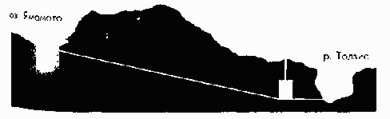
\includegraphics[scale=0.5]{figures/fig-14.png}

на плане проложена так. Но Гото Денго, не меняя чертежей, приказал, чтобы на самом деле ее проходили так:

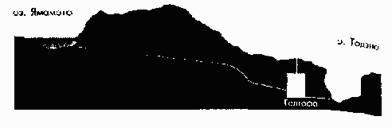
\includegraphics[scale=0.5]{figures/fig-15.png}

Перегиб заметно удлинил туннель. Более того, порода скапливается в пологой западной части, и ее приходится выгребать вручную. О перегибе знают лишь сам Гото Денго, Ин и рабочие Ина. Истинное его назначение известно лишь Гото Денго.

--- Не надо напрямик. Продолжайте, как я сказал.

--- Да.

--- Кроме того, потребуется новая вентиляционная шахта.

--- Еще одна! Нет... --- протестует Ин.

Вентиляционные шахты, показанные на плане, с их жуткими изломами, отняли неимоверное количество сил.

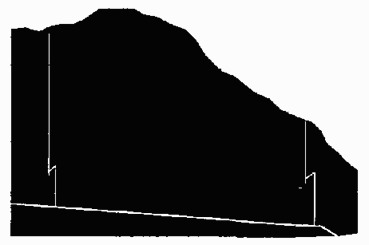
\includegraphics[scale=0.5]{figures/fig-16.png}

Однако Гото Денго несколько раз приказывал Ину и его команде начинать новые вентиляционные шахты, потом менял решение, и работа оставалась незаконченной.

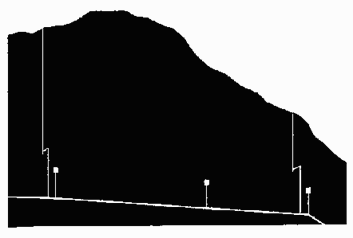
\includegraphics[scale=0.5]{figures/fig-17.png}

--- Новые вентиляционные шахты будем проходить сверху, --- говорит Гото Денго.

--- Нет! --- Ин в полном недоумении. Безумие пробивать вертикальный ствол сверху вниз и вытаскивать породу наверх. Если делать наоборот, она сама ссыплется вниз, и ее несложно откатить.

--- Получите еще помощников. Филиппинских рабочих.

Ин ошеломлен. Он еще больше, чем Гото Денго, отрезан от мира и должен догадываться о ходе войны по мучительно косвенным намекам. Заключенные складывают обрывки сведений в причудливые теории, настолько далекие от истины, что Гото Денго посмеялся бы, если бы сам не был в таком же положении. И он, и капитан Нода узнали, что Макартур высадился на Лейте, а японский флот разгромлен, только от генерала.

Одно Ин и другие рабочие угадали правильно: в Бандоке используют заключенных китайцев, чтобы обеспечить секретность. Если кто то из них сбежит, то окажется на острове, вдали от родины, среди людей, не говорящих на его языке и не питающих к нему особой приязни. То, что пригонят филиппинцев, наводит на размышления. Всю ночь китайцы будут перешептываться и строить догадки.

--- Нам не нужны еще рабочие. Мы почти закончили, --- говорит Ин. Гордость его снова уязвлена.

Гото Денго указательными пальцами постукивает себя по плечам, подразумевая эполеты. Ину требуется секунда, чтобы понять: речь о генерале. На его лице проступает заговорщицкое выражение. Он подходит на полшага ближе.

--- Приказы, --- говорит Гото Денго. --- Будем бить много вентиляционных шахт.

До прибытия в Бандок Ин не был шахтером, но теперь настоящий горняк и глубоко озадачен. Что немудрено.

--- Вентиляционные шахты? Куда?

--- Никуда, --- говорит Гото Денго.

На лице Ина по прежнему написано непонимание. Он думает, будто Гото Денго из за плохого знания шанхайского что то не так сказал. Но Гото Денго знает: Ин скоро додумается. Как нибудь ночью, в то тревожное время, которое всегда предшествует сну.

Тогда он поднимет мятеж. Люди лейтенанта Мори будут готовы: откроют огонь из минометов, взорвут мины, прочешут автоматными очередями тщательно спланированные сектора обстрела. Никто из рабочих не уцелеет.

Гото Денго этого не хочет. Он хлопает Ина по плечу.

--- Я дам тебе указания. Мы сделаем особую шахту.

С этими словами Гото Денго поворачивается и уходит; на нем еще маркшейдерские работы. Он знает: Ин успеет все вовремя сопоставить и спасти им жизнь.


Прибывают филиппинские заключенные. Колонны превратились в нестройные вереницы, люди волочат сбитые ноги, оставляя на дороге липкие красные следы. Японские солдаты, которые гонят их пинками и штыками, выглядят ненамного лучше. Гото Денго понимает, что заключенных гнали два дня без остановки, с тех самых пор, как получили приказ. Генерал обещал пятьсот новых работников. Дошло меньше трехсот. На носилках никого не тащат --- статистический нонсенс, учитывая их среднее физическое состояние. Понятно, что остальные двести обессилели по дороге и их добили на месте.

Бандок исключительно щедро снабжается горючим и провиантом. Гото Денго приказывает, чтобы заключенных и конвоиров одинаково хорошо покормили, и дает им день отдыха.

Потом отправляет на работу. Он уже давно руководит людьми, поэтому с ходу отбирает лучших. Среди новоприбывших есть некий Родольфо --- беззубый, пучеглазый, седой, с большим жировиком на щеке. У него непомерно длинные руки с кистями, как абордажные крючья, и растопыренные пальцы на ногах, как у дикарей, с которыми Гото Денго жил на Новой Гвинее. Невозможно сказать, какого цвета у него глаза --- они словно составлены из осколков чужих глаз, спеченных вместе серых, синих и карих искр. Родольфо стесняется отсутствия зубов; говоря, он всегда прикрывает ладонью рот. Как только подходит Гото Денго или еще кто нибудь из начальства, молодые филиппинцы, словно по команде, отводят глаза и смотрят на Родольфо --- тот выступает вперед, прикрывается ладонью и устремляет на посетителя свой странный, нервирующий взгляд.

--- Разбейте людей на шесть бригад, присвойте им названия и назначьте старших. Каждый должен знать название своей бригады и фамилию бригадира, --- довольно громко говорит Гото Денго. По крайней мере часть других филиппинцев наверняка понимают по английски. Потом подается ближе и понижает голос: --- Несколько самых лучших и сильных оставь себе.

Родольфо моргает, застывает по военному, убирает руку ото рта и отдает честь. Корявая лапища, как навес, отбрасывает тень на лицо и грудь. Видно, что козырять он научился у американцев. Поворачивается кругом.

--- Родольфо.

Родольфо оборачивается с такой досадой, что Гото Денго еле сдерживает смех.

--- Макартур на Лейте.

Грудь у Родольфо раздувается, как аэростат, он вырастает на три дюйма, но выражение лица не меняется.

Весть молнией разносится по филиппинскому лагерю. Тактика достигает цели: филиппинцам снова есть ради чего жить; в них просыпаются энтузиазм и энергия.

На повозках, запряженных буйволами, прибывают изношенные перфораторы и компрессоры, надо полагать, с другого такого же участка на Лусоне. Филиппинцы --- специалисты по внутреннему сгоранию --- раскурочивают часть компрессоров, чтобы починить остальные. Перфораторы раздают по бригадам. Филиппинцы поднимаются на водоразделы и начинают проходить <<вентиляционные шахты>>; китайцы тем временем заканчивают комплекс Голгофы.

Повозки попросту реквизировали на дороге вместе с погонщиками --- по большей части крестьянами, которых забрили прямо на месте. Разумеется, домой их не отпускают. Самых слабых буйволов забивают на мясо, тех, что посильнее, отправляют вывозить пустую породу, погонщиков присоединяют к рабочим. Среди них есть парнишка по имени Хуан, круглолицый, с явной примесью китайской крови. Он одинаково хорошо говорит на английском, тагальском и кантонском. С Ином и другими китайцами он объясняется на своего рода пиджине, часто рисуя иероглифы пальцем на ладони. Хуан маленький, жилистый и прыткий. Гото Денго решает, что это может пригодиться впоследствии, и отбирает его в особую команду.

Зацементированное устье штольни на дне озера Ямамото надо осмотреть. Гото Денго спрашивает у Родольфо, нет ли среди филиппинцев бывших ловцов жемчуга. Довольно быстро отыскивается тощий, хлипкого вида палаванец по имени Августин. Он ослабел от дизентерии, но при виде воды как будто оживает. После двух дней отдыха он легко спускается на дно озера Ямамото. Его Родольфо тоже берет в свою команду.

Инструмента и шахт на всех филиппинцев не хватает, поэтому они часто сменяются, и работа продвигается быстро. И вот однажды, в два часа ночи, джунгли оглашаются непривычным звуком. Он доносится из низин, где река Тодзио петляет среди рисовых полей и плантаций сахарного тростника.

Это звук моторов. Множества моторов. Японцы несколько месяцев сидят без горючего, и первая мысль Гото Денго, что это Макартур.

Он торопливо натягивает форму и вместе с другими офицерами выбегает к главным воротам Бандока. Здесь выстроилась очередь из десятков грузовиков и нескольких легковых автомобилей, моторы работают, фары выключены. Гото Денго слышит японскую речь и падает духом. Он уже давно не стыдится, что ждет генерала Дугласа Макартура как избавителя.

В грузовиках приехали солдаты. Когда встает солнце, Гото Денго предстает новое и необычное зрелище: свежие, здоровые, сытые японцы. Они вооружены автоматами и похожи на японских солдат в 37 м, во время победного шествия по Северному Китаю. Гото Денго чувствует странную ностальгию по времени, когда впереди не маячило неминуемое поражение и чудовищный крах. В горле встает комок, в носу щиплет.

И тут же он отбрасывает эти мысли, вспомнив, что великий день все таки наступил. У той его части, которая по прежнему верна Императору, есть долг: разместить жизненно важные военные припасы в большой камере Голгофы. Той части, которая уже не верна Императору, тоже многое предстоит сделать.

На войне, сколько ни планируй, ни готовься, ни отрабатывай на учениях, когда наступает великий день, все неизбежно идет наперекосяк. Сегодня не исключение. Однако через несколько часов неразберихи все налаживается, люди усваивают свои роли. Самые большие грузовики не могут пройти по дороге, которую Гото Денго построил в русле реки Тодзио, но два маленьких проезжают. Они становятся челноками. Большие грузовики подъезжают, один за другим, к сооруженному несколько месяцев назад мощному оборонительному периметру --- надежно укрытому от самолетов разведчиков Макартура. Филиппинцы облепляют их и разгружают ящики --- маленькие, явно очень тяжелые. Тем временем грузовички поменьше курсируют по реке Тодзио к устью Голгофы: там ящики перегружают в вагонетки и закатывают в главную камеру. По указанию сверху каждый двадцатый ящик Гото Денго отправляет в ложную камеру. Дальше разгрузка идет сама собой, и Гото Денго большую часть времени присматривает за последними стадиями работ. Новые вентиляционные шахты продвигаются по графику, их можно инспектировать раз в день. Диагональную штольню теперь отделяют от озера Ямамото всего несколько метров. Грунтовые воды сочатся в Голгофу сквозь мелкие трещинки в породе и стекают в зумпф, который дренируется в реку Тодзио. Еще несколько метров, и они соединятся с коротким туннелем, который Ин и его люди пробили несколько месяцев назад из того места, где теперь дно озера Ямамото.

Ин теперь занят на других работах. Они с Родольфо и спецкомандой заканчивают последние приготовления: бьют выработку с вершины водораздела. Она выглядит в точности как очередная вентиляционная шахта.

Гото Денго совершенно потерял счет дням, однако через четыре дня после прибытия грузовиков он получает намек. За вечерним рисом филиппинские рабочие внезапно затягивают песню. Гото Денго узнает мелодию: как то ее пели американские морские пехотинцы в Шанхае.


Что за младенец

Тихо спит

В объятьях у Марии?


Филиппинцы поют эту и другие песни на английском, испанском и латыни весь вечер. Когда они прочистят легкие, то поют исключительно красиво на два или на три голоса. Поначалу солдаты лейтенанта Мори нервничают, думая, что это сигнал к массовым беспорядкам. Гото Денго не хочет, чтобы перебили его рабочих, и объясняет, что это религиозное --- мирный праздник.

В ту ночь приезжает еще один караван грузовиков. Заключенных будят и отправляют на разгрузку. Они работают весело, поют рождественские гимны и шутят насчет Санта Клауса.

Разгрузка продолжается всю ночь и утром после рассвета. Никто в лагере не спит. Впрочем, Бандок и так постепенно переходит на ночной график, чтобы меньше было видно с самолетов разведчиков. Гото Денго как раз думает, не прикорнуть ли на часок, когда со стороны реки Тодзио доносится треск. Патронов мало, он давно не слышал этого звука и с трудом понимает, что стреляют из <<намбу>>.

Гото вспрыгивает на подножку грузовика и велит водителю ехать вверх. Стрельба смолкает так же внезапно, как началась. Река под лысыми шинами грузовика стала красной и мутной.

Примерно два десятка тел лежат в реке перед устьем Голгофы. Японские солдаты стоят по щиколотку в красной воде. В руках у них автоматы. Сержант обходит лежащих филиппинцев добивая штыком тех, кто еще шевелится.

--- Что происходит? --- спрашивает Гото Денго. Никто не отвечает. Впрочем, в него не стреляют; значит, он может выяснить сам.

Заключенные разгружали грузовичок --- он по прежнему стоит перед устьем штольни. Под задним откидным бортом лежит ящик. Видимо, его уронили, он раскололся под весом содержимого, и оно рассыпалось по конгломерату из речных камней, цемента и отвала штольни, слагающих здесь ложе реки.

Гото Денго подходит, плеща по воде. Всё перед глазами, но он почему то не может впитать увиденное, пока не пощупает руками. Он нагибается, обхватывает пальцами холодный брусок и вынимает его из воды. Это блестящий слиток желтого металла, необычайно тяжелый, с вдавленным клеймом: <<БАНК СИНГАПУРА>>.

Сзади раздается шум. Сержант стоит на изготовку, двое солдат вытаскивают из кабины филиппинца, который привез Гото Денго. Спокойно --- почти скучающе --- сержант закалывает водителя, и солдаты бросают его в красную воду. <<Веселого Рождества>>, --- шутит один солдат. Все смеются, за исключением Гото Денго.


\chapter{ИМПУЛЬС}


На обратном пути через дом Ави бросает на иврите что то ветхозаветное, отчего дети заливаются слезами, а няни вскакивают с ковра и начинают запихивать вещи в сумки. Из спальни выходит заспанная Дебора. Они с Ави нежно обнимаются в прихожей. Рэнди чувствует себя совершенно лишним, поэтому, не заходя в дом, садится в машину и жмет на газ. Он едет через холмы над разломом Сан Андреас, потом сворачивает к югу. Через десять минут по левой полосе на скорости девяносто сто миль в час проносится машина Ави. Рэнди едва успевает прочесть наклейку на бампере: <<МЫ НЕ ЖЛОБЫ, ЖЛОБЫ НЕ МЫ>>.

Рэнди ищет место, откуда можно анонимно выйти в Интернет. Гостиница не годится, в гостиницах регистрируются все исходящие звонки. На самом деле лучше всего воспользоваться интерфейсом пакетной радиосвязи в ноутбуке, но и для этого надо где то сесть, чтобы не тревожили. Сгодился бы фаст фуд, однако в здешних голых и пустынных краях их днем с огнем не сыщешь. Добравшись до северного края долины --- Менло Парка и Пало Альто, Рэнди решает, что гори оно все синим огнем, надо ехать прямо на место действия. Может, он там еще зачем пригодится. Поэтому Рэнди сворачивает с основной дороги и едет в деловую часть Лос Альтоса, симпатичного послевоенного городка, постепенно захватываемого франшизами. Главный проспект косо пересекает деловая улочка, образуя два маленьких (остроугольных) участка и два (больших) тупоугольных. На одной стороне проспекта тупой угол занимает офисное здание, где разместились <<Новус Ордо Секлорум>> и Гроб. В остром углу --- <<Макдоналдс>>. С противоположной стороны тупой угол, по странному совпадению, занимает универмаг <<24 часа>>, единственный, который Рэнди пока видел в Западном полушарии. В остром углу расположилась автомобильная парковка, на которой можно оставить машину, чтобы по старинке прогуляться от магазинчика к магазинчику.

Стоянка перед <<Макдоналдсом>> заполнена, поэтому Рэнди подъезжает к уличному окошку, выбирает n, где n --- произвольное число от одного до шести, и заказывает <<Обед номер n >> с супербольшой порцией картошки. Получив искомое, он гонит через улицу на парковку. Под самым его носом последнее свободное место занимает микроавтобус с логотипом телекомпании из Сан Хосе. Рэнди не собирается далеко уходить, поэтому просто перегораживает выезд другому автомобилю, но в последний миг замечает там движение и видит, что сидящий в машине длинноволосый бородач методично заряжает помповое ружье. Бородач видит Рэнди в зеркальце заднего вида и оборачивается с безукоризненно вежливой миной типа <<простите, сэр, но вы загородили мне выезд>>. Рэнди узнает бородача: это то ли Майк, то ли Марк, специалист по графическим адаптерам, который разводит устриц в Гилрое (в мире высоких технологий популярны экзотические хобби). Рэнди отъезжает и останавливается снова, загородив выезд фургону, который, судя по виду, стоит тут с середины семидесятых.

Он залезает на крышу <<акуры>>, прихватив ноутбук и <<Обед номер n >>. Раньше он бы никогда не стал сидеть на своей машине, чтобы не продавить металл. Однако с тех пор как Ами протаранила ее грузовиком, Рэнди стал несколько менее занудным и теперь смотрит на автомобиль как на инструмент, которым надо пользоваться, пока он не превратился в груду металлолома. У Рэнди есть двенадцативольтовый адаптер, и он подключает его к прикуривателю. Теперь, когда все готово, можно и осмотреться.

Парковка перед зданием <<Новус Ордо Секлорум>> забита полицейскими машинами, а также <<мерседесами>> и <<БМВ>>, в которых, надо думать, приехали адвокаты. <<Рейнджровер>> Ави лихо поставлен прямо на газоне, там же разместились несколько съемочных групп. На пятачке перед входом столпилась куча народа, все друг на друга орут. Их окружают полиция, пресса и адвокатские шестерки --- собирательно, те, кого Толкин назвал бы людьми. Здесь же присутствуют не --- и постчеловеческие создания, наделенные своеобразной внешностью и кое какими чарами: гномы (упорные, немногословные труженики) и эльфы (более воздушные и блистательные). Рэнди, гном, недавно начал понимать, что его дед, вероятно, был эльфом. Ави --- человек с сильным эльфийским ореолом. Где то, очевидно, в самой давке --- Голлум.

На экране ноутбука есть окошко, в котором крутится стилизованная под старый новостной ролик анимация: радиобашня, излучающая концептуальные радиоволны по всей планете, показанной исключительно вне масштаба: диаметр Земли почти равен высоте башни. То, что Зевсовы инфо громы видны и движутся, означает, что радиоадаптер сумел подключиться к пакетной радиосети. Рэнди открывает терминальное окошко, печатает:


telnet laundry.org


и через несколько секунд --- бах! --- появляется приглашение ввести пароль. Рэнди снова смотрит на анимацию и с удовлетворением видит, что инфо громы сменились залпами вопросительных знаков. Значит, его компьютер опознал laundry.org как машину, поддерживающую протокол S/WAN --- т.е, что каждый пакет, идущий от ноутбука Рэнди к laundry.org или обратно, зашифрован. Определенно неплохая идейка, когда собираешься сделать по радио что то противозаконное.

Майк или Марк выбирается из машины. Театральный эффект от длинного черного пальто несколько портит надетая под него черная футболка с жирным вопросительным знаком. Он забрасывает ружье на плечо, наклоняется, берет с сиденья черную ковбойскую шляпу и кладет ее на крышу машины, потом запрокидывает голову и, глядя в небо, заправляет длинные носы за уши. Нахлобучивает шляпу, снимает с шеи черный платок вес с тем же вопросительным знаком и завязывает лицо, так что между шляпой и платком остается лишь узкая щель для глаз. Рэнди бы струхнул, если бы несколько его друзей, включая Джона Кантрелла, не имели обыкновения расхаживать в таком виде. Майк или Марк идет через стоянку --- один из телеоператоров следит за ним камерой --- к универмагу.

Рэнди входит в ssh (secure shell, или безопасное соединение) laundry.org --- способ дополнительно защитить обмен между двумя компьютерами. Laundry.org --- анонимизирующий прокси сервер. Любой пакет, направляемый с него на другой компьютер, первым делом освобождается от всякой дополнительной информации; если его и перехватят, нельзя будет сказать, откуда он послан. Соединившись с прокси, Рэнди печатает:


telnet crypt.kk


нажимает <<ввод>> и потом буквально молится. Крипта все еще в состоянии утряски (разумеется, только поэтому содержимое Гроба еще не перекачали в нее).

На стоянке перед универмагом Майк или Марк присоединяется к еще трем эльфийского вида чувакам с завязанными лицами и в черных ковбойских шляпах. Рэнди узнает их по длине и цвету бород и <<хвостов>>. Это Стью, аспирант из Беркли, как то завязанный в проект Ави насчет ППХ, Фил, который несколько лет назад изобрел новый язык программирования, а в свободное время катается на лыжах с недоступных гор, и Крег --- он знает все про шифрование операций с кредитными карточками в Сети и увлекается традиционной японской стрельбой из лука. Кто то из них в длинном пальто, кто то нет. Много символики Тайных Обожателей: футболки с числом 56, кодом Ямамото, портреты самого Ямамото или просто жирные красные вопросительные знаки. Они что то бурно и весело обсуждают, что, впрочем, выглядит несколько наигранным, потому что у одного за спиной охотничий карабин, у двух других --- рудиментарного вида ружья с торчащим вбок магазином, как у АК 47. Рэнди думает, но не уверен, что это винтовки ППХ.

Группа, ясное дело, привлекла внимание полицейских, которые окружили четверку патрульными машинами и стоят с помповыми ружьями наготове. В большинстве штатов существуют странные законы: чтобы носить (например) спрятанный однозарядный пистолет 22 го калибра, нужна лицензия, а вот (например) с охотничьим карабином можно ходить свободно. Спрятанное оружие запрещено или строго регламентируется носимое на виду --- нет. Поэтому Тайные Обожатели (многие из них помешаны на огнестрельном оружии) взяли за правило расхаживать с ружьями, чтобы показать абсурдность таких правил. Суть их аргументов такова: на черта носить при себе спрятанный револьвер, годный только против разбойного нападения, которое в жизни практически не случается? Конституция дает право носить оружие исключительно для защиты от неправедного правительства, а когда такое происходит, револьвер бесполезен. Поэтому (считают ребята) если уж осуществлять свое право на ношение оружия, так делать это в открытую и не размениваться на мелочи.

По экрану бежит всякая муть. Она начинается со слов <<ДОБРО ПОЖАЛОВАТЬ В КРИПТУ>>, дальше идет инфа о том, какая это классная штука и как всякий, кого хоть сколько нибудь колышет защита информации, должен открыть в ней счет. Рэнди нажатием клавиши пресекает рекламу и входит как Рэнди. Потом вводит команду:


telnet tombstone.epiphyte.com


и получает в ответ два радующих сообщения: что установлена связь с Гробом и что автоматически согласовано соединение S/WAN. Наконец он получает:


tombstone login:


это значит, что он может войти в компьютер на противоположной стороне улицы. И теперь надо принимать решение.

Пока он чист. Биты, идущие с его ноутбука, зашифрованы; если кто то и прослушивает местную сеть пакетной радиосвязи, он знает только, что вокруг витают зашифрованные биты. Чтобы проследить, откуда они идут, надо направить на Рэнди немалых размеров сложный радиопеленгатор. Зашифрованные биты попадают на laundry.org в Окленде: огромный сервер, через который каждую секунду проходят тысячи пакетов. Если кто то, не жалея оборудования и средств (поскольку дело это дорогостоящее), прослушивает Т3 канал laundry.org, он узнает только, что небольшое количество зашифрованных пакетов ушло на адрес crypt.kk в Кинакуте. Однако из laundry.org эти пакеты вышли без опознавательных признаков. В свою очередь, crypt.kk --- тоже анонимайзер: некто или нечто, прослушивающее ее мощный канал T5 (работа для телекоммуникационной системы небольшого государства), теоретически мог бы различить обмен пакетами между crypt.kk и Гробом. Но опять таки все они лишены опознавательных признаков, так что невозможно проследить их даже до laundry.org, не говоря уже о компьютере Рэнди.

А вот чтобы войти в Гроб и по настоящему уничтожить улики, надо ввести имя пользователя. Будь это плохо защищенный сервер, каких в Интернете тьма, Рэнди просто воспользовался бы какой нибудь из бесконечных дырок в защите и вошел несанкционированно. Тогда в случае чего можно было бы отпереться: Мол, какой то неведомый хакер случайно взломал сервер в ту минуту, когда его изымала полиция. Но Рэнди посвятил последние несколько лет жизни тому, чтобы сделать такие машины неуязвимыми, и знает, что это невозможно.

Более того, нет смысла входить как обычный пользователь, например, с гостевого входа. Гостям не позволяют копаться в системных файлах. Чтобы уничтожить улики, Рэнди должен войти как суперюзер. Имя суперюзера, к несчастью, <<randy>>, и нельзя войти как <<randy>>, не вводя пароль, который, кроме него, никто не знает. Так что, воспользовавшись самыми современными криптографическими методиками и трансокеанской пакетной радиосвязью, Рэнди оказался перед необходимостью ввести в чертов компьютер свое имя.

В голове проносится короткий сценарий, в котором он, Рэнди, рассылает сообщение всем пользователям laundry.org: <<пароль пользователя randy на tombstone.epiphyte.com такой то, просьба как можно скорее распространить эту информацию по всему Интернету>>. Идейка была бы стоящая, приди она ему в голову час назад. Теперь поздно: любой вменяемый прокурор, сличив время, докажет, что это сделано для отвода глаз. И потом, надо поторапливаться. Перепалка у входа, звучавшая приглушенным гулом, становится громче и яростнее.

Рэнди тем временем запустил браузер и зашел на домашнюю страничку ordo.net. Обычно это довольно скучный корпоративный сайт, однако сегодня будничные пресс релизы и краткие аннотации уступили место окну, где идет живой видеопоказ происходящего перед входом (вернее, того, что происходило там секунды две назад; радиоканал хиленький и фреймы сменяются раз в три секунды). Трансляция идет из самого <<Ордо>>: надо думать, ребята выставили камеру в окно и передают изображение по собственному каналу Т3.

Рэнди отрывает взгляд от экрана как раз вовремя, чтобы увидеть, как через стоянку, увлеченно беседуя с главным редактором журнала <<Тьюринг>>, идет человек, придумавший термин <<виртуальная реальность>>. Их догоняет Брюс, инженер по операционным системам, который на досуге записывает народную музыку аборигенов Огненной Земли и бесплатно распространяет ее через Интернет.

--- Брюс! --- кричит Рэнди.

Брюс замедляет шаг и поднимает голову.

--- Рэнди, --- говорит он.

--- Как ты здесь оказался?

--- Пронесся слух, что федералы штурмуют <<Ордо>>.

--- Интересно... какие нибудь определенные федералы?

--- Комсток, --- говорит Брюс. Он имеет в виду Пола Комстока, Генерального прокурора США, которому подчиняется ФБР. Рэнди не верит, тем не менее машинально всматривается в толпу, выискивая взглядом фэбээровцев. ФБР ненавидит мощную криптографию и боится ее. Кто то из Тайных Обожателей кричит: <<Я слышал, Секретная служба!>>. Это еще более зловеще, потому что Секретная служба, агентство в структуре министерства финансов, призвана бороться с электронными махинациями и защищать национальную валюту.

Рэнди говорит:

--- А ты не думаешь, что это <<утка>>? Что просто в <<Ордо>> изымают оборудование из за каких то судебных дрязг?

--- Тогда зачем здесь столько полицейских? --- спрашивает Брюс.

--- Может, из за вооруженных людей с завязанными лицами?

--- А чего бы Тайные Обожатели сбежались, не будь это правительственный рейд?

--- Не знаю. Может быть, какой то феномен спонтанной самоорганизации вроде зарождения жизни в первичном бульоне.

Брюс говорит:

--- А вдруг юридические дрязги --- только предлог?

--- Этакий троянский конь, сооруженный Комстоком?

--- Да.

--- Зная все участвующие стороны, я сильно в этом сомневаюсь, --- говорит Рэнди, --- хотя надо подумать.

Перепалка на стоянке <<Ордо>> становится все более ожесточенной. Рэнди смотрит на видеоокошко, в котором, к сожалению, нет саундтрека. Смена фреймов происходит так: изолированные группы пикселей одна за другой выскакивают на старом изображении, как будто большой рекламный щит заклеивают по частям. Это тебе не телевидение высокого разрешения. Тем не менее Рэнди определенно различает Ави: он стоит, высокий, бледный и спокойный, между какими то двумя типами. Один, видимо, Лэйв, президент <<Ордо>>, другой, надо полагать, адвокат. Они буквально преграждают вход в здание двум полицейским и лично Эндрю Лоубу. Последний движется быстро и потому представляет собой непосильную задачу для пропускной способности канала. Интернетовская видеосистема достаточно умна, чтобы не возиться с почти неподвижными частями изображения: вросшие в землю полицейские обновляются раза два за минуту, и то фрагментарно. Однако Эндрю Лоуб размахивает руками, подпрыгивает, кидается на Ави, отскакивает назад, подносит к уху сотовый и трясет в воздухе документами. Компьютер определил его как набор пикселей, требующий особого внимания и пропускной способности, соответственно какой то хиленький алгоритм, изнемогая под натиском сжатых пикселей, составляющих изображение Эндрю Лоуба, из последних сил фиксирует наиболее быстро движущиеся части в дискретные фреймы, рубит их на квадратики и отправляет в виде пакетов по сети. Пакеты попадают на компьютер Рэнди так, как передает их радиосвязь, то есть спорадически и в неверном порядке. Эндрю Лоуб предстает кубистическим глюком цифрового видео, схематической амебой преимущественно пальтово бежевых пикселей. Время от времени рот или глаза материализуются отдельно от тела и на несколько секунд застывают в немой ярости.

Картинка гипнотизирует. Из транса Рэнди выводит резкий звук. Оказывается, фургон позади его машины не брошенный: он полон гномами, которые теперь открыли задние двери, так что виден клубок проводов и кабелей. Двое гномов затаскивают на крышу фургона тяжелый прямоугольный агрегат. Провода соединяют его с другим, явно электрическим, агрегатом внизу. Не похоже, что из него можно стрелять, и Рэнди решает пока не отвлекаться.

С другой стороны улицы доносятся крики. Рэнди видит, как из полицейского фургона вылезают копы с тараном.

Рэнди печатает:


randy


И нажимает ввод. Гроб отвечает:


password:


и Рэнди вводит пароль. Гроб сообщает, что он вошел в систему и для него есть почта.

То, что Рэнди вошел в систему, сейчас записано в нескольких местах жесткого диска. Другими словами, он только что оставил жирные отпечатки пальцев на орудии, которое вот вот изымет полиция. Если Гроб отключат и вынесут раньше, чем Рэнди успеет стереть следы, полиция узнает, что он входил в компьютер в самый момент конфискации. Это дело пахнет тюремным сроком. Жалко, Дуглас Макартур Шафто не видит, какую крутую штуку он сейчас проделывает. С другой стороны, Дуг наверняка проделывает всякие крутые штуки, о которых Рэнди ничего не известно, и Рэнди все равно его уважает, просто за то, как он себя держит. Может, чтобы так себя держать, надо, не афишируя проделывать всякие крутые штуки, и тогда это каким то образом проступает сквозь твою внешнюю оболочку.

Рэнди может просто отформатировать весь жесткий диск одной командой, но (1) потребуется несколько минут, и (2) информация не уничтожится полностью; любой специалист сможет ее восстановить. Рэнди знает, в каких файлах зафиксировано его посещение, и запускает команду поиска этих файлов на диске. Затем печатает команду, по которой эти участки диска будут заполнены случайными числами семь раз кряду.

Рэнди нажимает <<ввод>>, полицейские тем временем бьют тараном в боковую дверь здания. Теперь его практически нельзя обвинить в уничтожении улик, но он еще ничего не уничтожил, а без этого не стоило и огород городить. Нужно отыскать копии всех электронных писем с координатами подлодки и проделать над ними ту же многократную перезапись. Будь эта дрянь не зашифрована, он бы искал нужную последовательность цифр; а так придется искать файлы, созданные в определенный период времени, когда Рэнди отправлял письма с <<Глории>>, стоящей на якоре над подлодкой. Он примерно помнит дату и для надежности задает поиск в интервале плюс минус пять дней, ограничивая его директориями, отведенными под электронную почту.

Поиск длится вечность или так кажется, потому что копы уже снесли дверь и ворвались в здание. Видеоокошко резко меняется: теперь это монтаж из холла, дверного проема, приемной и, наконец, баррикады. Ребята перетащили камеру от окна на стол у входа. Теперь в окошке груда дешевой офисной мебели, наваленная перед стеклянными дверьми приемной. Камера идет вверх, показывая, что стеклянные двери уже пошли сеткой трещин от (надо думать) удара тараном.

Команда <<find>> возвращается со списком из примерно ста файлов. Пять шесть --- те самые, с координатами, но Рэнди уже некогда их вычислять. Он запрашивает список блоков на диске, занятых этими файлами, чтобы потом стереть их тщательнее, затем применяет ко всем команду <<rm>> --- удалить. Это жалкий и ненадежный способ стереть информацию с жесткого диска, однако Рэнди боится, что ничего другого не успеет. Выполнение <<rm>> занимает всего несколько мгновений; после этого Рэнди дает команду забить блоки случайными цифрами семь раз кряду, как прошлый раз. Баррикада уже разметана по всему холлу и копы в самом здании. Вид у них мрачный, они держат автоматы наготове, дулами в потолок.

Остается еще одно дело, причем не быстрое. Эпифитовцы используют Гроб для самых разных целей, и кто знает, не хранятся ли там еще копии широты и долготы. Большинство руководящего состава --- старые компьютерные волки, с которых вполне станется составить маленькую программку для еженедельной архивации всей почты. Поэтому Рэнди быстренько набивает свою программку, которая напишет случайную информацию во все сектора всего жесткого диска, потом вернется и сделает это снова, и снова, и снова, и так до бесконечности или пока полицейские не выдернут шнур. Он нажимает <<ввод>>, и тут со стороны фургона доносится электрический треск, от которого волосы на голове встают дыбом. Полицейский в видеоокошке застывает. В следующий миг экран чернеет.

Рэнди оборачивается на старый фургон. Гномы победно жмут друг другу руки.

Слышится скрежет шин и грохот сталкивающихся на малой скорости автомобилей. С десяток машин плавно остановились, часть исправных въехали им в зад. В <<Макдоналдсе>> погас свет. Телеоператоры чертыхаются над своим оборудованием. Полицейские офицеры и адвокаты стучат рациями и сотовыми по ладоням.

--- Простите, джентльмены, --- обращается Рэнди к гномам, --- не объясните ли вы, что происходит?

--- Мы только что вырубили все здание, --- говорит один.

--- В каком смысле?

--- Звезданули по нему мощным электромагнитным импульсом. Спалили все чипы в пределах досягаемости.

--- Тактика выжженной земли? Конфискуйте что хотите, паршивые федералы, теперь это бесполезный металлолом?

--- Да.

--- Что же, на автомобили точно подействовало, --- говорит Рэнди. --- И на тот металлолом, который прежде был моим компом.

--- Не боись, жестким дискам это не вредит, --- успокаивает гном, --- так что все твои файлы целы.

--- Понимаю, что вы хотели меня обрадовать, --- говорит Рэнди.


\chapter{БУДДА}


Подъезжает машина. Звук двигателя старательно заглушен, но похоже, что это дизель. Гото Денго не спит, ждет, как и весь остальной лагерь. Днем в Бандоке заняты только радисты и зенитчики. Никто не сообщил, что Макартур на Лусоне хотя присутствие генерала ощущается. Американские самолеты дни напролет рассекают небо, блестящие и гордые, словно звездолеты из далекого будущего, которого никому из них не увидеть; земля гудит, как колокол, от залпов далеких линкоров. <<Материал>> завозят меньшими партиями, один два раздолбанных грузовичка за ночь, задние бамперы едва не скребут дорогу под непосильным бременем золота.

Лейтенант Мори поставил пулемет за густой листвой у главного въезда --- на случай, если сюда ненароком занесет американцев на джипе. Где то в темноте пулеметное дуло следит за подъезжающей машиной. Часовые знают каждую выбоину на дороге и угадывают положение машины по скрежету ходовой части о камни, характерной последовательности металлических точек и тире.

Фары у машины, естественно, выключены, часовые у ворот не смеют зажигать яркий огонь. Кто то отваживается приоткрыть керосиновую лампу и направить луч на посетителей. Из тьмы возникает серебристая эмблема <<мерседес бенц>> над хромированным радиатором. Луч лампы скользит по черным крыльям автомобиля, серебристым выхлопным трубам, подножкам, заляпанным молодой кокосовой мякотью --- видимо, автомобиль по дороге задел груду орехов. На водительском месте японец лет сорока пятидесяти, такой усталый и осунувшийся, что кажется --- сейчас зальется слезами. Но это всего лишь шофер. Рядом сержант с обрезом --- японские ружья такие длинные, что на переднем сиденье шикарного автомобиля с ними не развернешься. Кто или что на заднем сиденье, не видно --- оно задернуто занавеской.

--- Открой! --- требует солдат, и водитель, заведя руку за голову, раздвигает занавески. Луч лампы ударяет в щель и вспыхивает на бледном лице пассажира. Несколько часовых вскрикивают. Гото Денго ошалело пятится, потом подходит ближе, чтобы всмотреться.

У человека на заднем сиденье огромная голова в странном островерхом уборе, но удивительнее всего кожа: не желтоватая, как у обычного монголоида, а ярко желтая и блестящая. На губах играет спокойная улыбка --- Гото Денго не видел такой с начала войны.

Вспыхивают еще огни, вкруг машины сжимается кольцо солдат и офицеров. Кто то распахивает главную дверь и отшатывается, словно обжегся о ручку.

Пассажир сидит скрестив ноги, сиденье прогнулось под его весом почти до пола.

Это цельнозолотой Будда --- трофей из каких то других краев Зоны Совместного Процветания Великой Азии. Он прибыл, чтобы безмятежно медитировать на груде сокровищ в сердце Голгофы.

В устье штольни Будда пролезает, однако в вагонетку не помешается, и несколько самых сильных филиппинцев несколько часов дюйм за дюймом толкают его по туннелю.

Поначалу золото везли в крепких ящиках с надписями <<патроны>>, <<мины>> и тому подобное. Потом пошли ящики без маркировки. С какого то момента их сменили картонные коробки и чемоданы. Они все время рвутся; заключенные терпеливо собирают золото, несут к устью штольни и бросают в вагонетки. Слитки ударяются с грохотом, от которого с деревьев взлетают тучи перепуганных птиц. Гото Денго поневоле засматривается на слитки. Они разного размера (иные приходится тащить вдвоем), с клеймами банков из таких мест, где Гото Денго бывал, но чаще --- из таких, о которых он только слышал: Сингапур, Сайгон, Батавия, Манила, Рангун, Гонконг, Шанхай, Кантон. Есть французское золото, вывезенное в Камбоджу, голландское --- в Джакарту, британское --- в Сингапур, все для того, чтоб оно не досталось немцам.

Некоторые партии целиком составляет золото из Токийского банка. Его привозят пять караванов подряд. Согласно описи, которую Гото Денго ведет у себя в голове, две трети сокровищ Голгофы поступили непосредственно из центрального резерва Японии. Золото холодное на ощупь и уложено в крепкие старые ящики. Надо думать, оно дожидалось этого часа в каком нибудь манильском подвале. Видимо, на Филиппины его доставили примерно тогда же, когда Гото Денго вывезли с Новой Гвинеи, в конце сорок третьего.

Они знали. Они уже тогда знали, что проигрывают войну.

К середине января Гото Денго вспоминает рождественскую резню с какой то почти ностальгией по наивному неведению, сделавшему убийство необходимым. До того утра даже он мог убедить себя, что Голгофа --- склад оружия, которым императорские солдаты когда нибудь отвоюют Лусон. Верили в это и заключенные. Теперь все знают про золото, и настроение изменилось. Ясно: отсюда живым не выйти.

К началу января заключенные разделились на две категории одни смирились со своей участью, другие --- нет. Непокорные предпринимают несколько стихийных попыток к бегству и гибнут под пулями. Патроны больше не экономят, а может, охранники слишком измотаны и голодны, чтобы спускаться с вышки и лично закалывать штыком каждого, кто напрашивается. Беглецов просто расстреливают, а тела оставляют чернеть и раздуваться. Весь Бандок пронизан их смрадом.

Впрочем, Гото Денго почти не замечает вони, потому что в атмосфере лагеря висит безумное, томительное напряжение, которое всегда предшествует бою. Или так ему кажется; он много чего испытал на войне, но ни разу не был в настоящем бою. То же распространяется на всех его соотечественников в Бандоке; японцы, побывавшие в бою, по большей части мертвы. В этой армии ты или зеленый новичок, или покойник.

Иногда вместе с золотом прибывает чемоданчик. Он всегда пристегнут наручниками к руке солдата, обвешанного гранатами, чтобы взорвать себя при нападении партизан. Чемоданчик отправляется прямиком на радиостанцию Бандока, и его содержимое прячут в сейф. Гото Денго догадывается, что там не обычные кодовые книги, а какие то особые однодневные шифры, поскольку каждое утро после восхода офицер радист выходит из домика, выполняет церемонию сожжения единственного листка бумаги и растирает пепел между пальцами.

Сюда, на радиостанцию, придет последний приказ. Все готово: Гото Денго раз в день обходит Голгофу с проверкой.

Две недели назад диагональную штольню наконец соединили с короткой выработкой на дне озера Ямамото. За несколько месяцев выработка наполнилась водой, просочившейся через цемент; когда два туннеля соединили, несколько тонн воды хлынуло в диагональную штольню. Этого ждали и были готовы: вода стекла в зумпф и оттуда в реку Тодзио. Теперь можно пройти вдоль всей штольни и посмотреть снизу на цементную затычку. За ней --- озеро Ямамото. Гото Денго ходит туда каждые два дня, якобы проинспектировать затычку и заложенную под нее взрывчатку, а на самом деле --- проверить, как продвигаются работы, которые, неведомо для капитана Ноды, ведут Ин и Родольфо с помощниками. Они по большей части пробивают все новые короткие слепые вертикальные стволы и расширяют выемки в их верхней части. Система (включая новые <<вентиляционные шахты>>, пробитые по указанию генерала) теперь выглядят так:

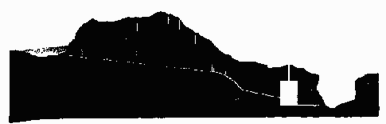
\includegraphics[scale=0.5]{figures/fig-11.png}

Внутри главного комплекса есть помещение, которое капитан Нода нарек Залом славы. Пока ничего славного здесь нет, только бесконечные провода сходятся сюда со всего подземного комплекса. Провода провешены под кровлей или тянутся по подошве и снабжены написанными от руки бирками, например <<ПОДРЫВНЫЕ ЗАРЯДЫ ГЛАВНОГО ВХОДА>>. Здесь же стоят несколько свинцовых аккумуляторов; их цель --- обеспечить энергию для детонации и дать Гото Денго несколько минут электрического света, чтобы прочесть бирки. В конце Зала славы сложены запасные ящики с динамитом и детонаторами на случай, если какие то туннели надо будет разрушить чуть более основательно, и мотки бикфордова шнура на случай, если не сработает электрическая цепь.

Однако приказ взрывать еще не прибыл, и Гото Денго делает то же, что любой солдат в ожидании смерти. Пишет близким письма, которые никогда не будут отправлены. Курит. Играет в карты. Снова и снова проверяет оборудование.

Проходит неделя, в течение которой золото не подвозят ни разу. Двадцать заключенных пытаются бежать вместе. Те, кто не подрывается на минной полосе, запутываются в колючей проволоке, и два солдата --- один с фонариком, другой с ружьем --- отстреливают их по очереди. Капитан Нода каждую ночь до рассвета расхаживает перед главными воротами, потом мертвецки напивается и ложится спать. Радисты сидят перед рациями, смотрят на светящиеся лампы и гальванически дергаются всякий раз, как на их частоте слышится слабый писк. Однако приказов все нет.

И вот однажды ночью снова, как в первый раз, приезжают грузовики. Видимо, это все японские машины, сколько их осталось на острове. Они гремят так, что слышно за полчаса до появления первого грузовика. Когда ящики вынимают и складывают на землю, солдаты, охранявшие колонну, остаются в Бандоке. Уезжают только водители.

На то, чтобы доставить в туннель последнюю партию золота, уходит два дня. Один из грузовичков безнадежно сломался, и его разобрали на запчасти, чтобы поддержать на ходу второй. У того не работает половина цилиндров, он еле тянет; заключенным приходится толкать его по дороге, а на самых трудных участках тащить тросами. Дожди все таки начались, река Тодзио поднимается.

Главная камера почти заполнена, ложная --- тоже. Новую партию приходится распихивать кое как: ящики взламывают и слитки засовывают в пустые промежутки. На ящиках --- орлы и свастики, сами слитки --- из Берлина, Вены, Варшавы, Праги, Парижа, Амстердама, Риги, Копенгагена, Будапешта, Бухареста, Милана. Еще есть картонные коробки с алмазами. Картон местами подмочен и пахнет морем. Гото Денго понимает, что из Германии недавно пришла большая подлодка с фашистской казной. Становится понятно, чего они две недели сидели без дела --- ждали эту самую лодку.

Два дня он, в шахтерской каске с фонариком, распихивает по щелям алмазы и золотые слитки. Он впал в своего рода транс, из которого его наконец выводит гулкий, прокатившийся по штольне грохот.

Артиллерия, думает Гото Денго. Или бомба с американского самолета.

Он по главной вентиляционной шахте выбирается на вершину водораздела. Там день. Внизу все спокойно, никакого боя. У Гото Денго падает сердце: Макартур его не спасет. Лейтенант Мори согнал наверх почти всех заключенных, они тросами втаскивают на гору оборудование и сбрасывают в недавно пробитые <<вентиляционные шахты>>. Здесь же оба грузовика: их кувалдами разбивают на куски, чтобы прошли в устье. Гото Денго успевает увидеть, как мотор электрогенератора радиостанции летит в черноту. Следом отправляется остальное радиооборудование.

Рядом, за деревьями, кто то тяжело сопит от натуги. Это сопение опытного бойца, от самой диафрагмы.

--- Лейтенант Гото! --- говорит капитан Нода. Он пьян в стельку. --- Ваше место внизу.

--- Что это был за грохот?

Нода ведет его на скальный выступ, откуда видна долина реки Тодзио. Гото Денго по многим причинам плохо соображает и сейчас едва не падает от внезапного головокружения. Дело в дезориентации: он не узнал реку. До сих пор это было сплетение струй в каменистом ущелье. Еще до того, как построили дорогу, можно было, прыгая с камня на камень, добраться почти до самого водопада. Теперь это широкая, глубокая, мутная река, из которой там и сям торчат верхушки каменных глыб.

Гото Денго вспоминает, как сто лет назад, в прошлом рождении, на другой планете видел простыню из гостиницы <<Манила>> с набросанным на ней планом. Реку Тодзио, проведенную жирной синей авторучкой.

--- Мы устроили обвал, --- говорит капитан Нода. --- Согласно плану.

Давным давно у пережима реки насыпали гору камней, чтобы после взрыва образовалась небольшая плотина. Однако взрывать динамит предполагалось непосредственно перед тем, как они замуруют себя внизу.

--- Но мы не готовы! --- говорит Гото Денго.

Нода смеется. Он в отличном настроении.

--- Вы уже месяц убеждаете меня, что все готово.

--- Да, --- медленно и хрипло отвечает Гото Денго. --- Вы правы. Все готово.

Нода хлопает его по спине.

--- Вы должны добраться до главного входа, пока его не затопило.

--- Мой взвод?

--- Дожидается там.

Гото Денго спешит по дороге к главному входу в штольню. По пути он минует еще одну вентиляционную шахту. Здесь под охраной солдат с примкнутыми штыками стоит вереница из нескольких десятков заключенных; руки у всех связаны за спиной проволокой. Один за другим филиппинцы опускаются на колени перед устьем. Лейтенант Мори с жутким сопением рассекает каждому шею офицерским мечом. Голова и тело падают в шахту и секунды через две глухо шмякаются на другие тела далеко внизу. Каждая травинка и камешек в радиусе трех метров пропитаны алой кровью, и лейтенант Мори --- тоже.

--- Об этом не беспокойтесь, --- говорит капитан Нода. --- Я прослежу, чтобы шахты засыпали щебнем, как мы и планировали. Джунгли скроют их раньше, чем американцы найдут это место.

Гото Денго отводит глаза и собирается идти.

--- Лейтенант Гото! --- раздается голос.

Гото Денго оборачивается. Это лейтенант Мори остановился перевести дух. Филиппинец, стоящий перед ним на коленях, бормочет латинскую молитву, за спиной перебирая четки связанными руками.

--- Да, лейтенант Мори.

--- Согласно моим спискам, за вами закреплено шесть заключенных. Они мне понадобятся.

--- Эти шестеро внизу, помогают разместить последнюю партию.

--- Вся последняя партия уже в туннеле.

--- Да, но не уложена. От ложной камеры не будет проку, если рассыпанные алмазы и золото приведут грабителя к главной. Мне нужны эти люди, чтобы завершить работу.

--- Вы берете на себя полную ответственность за них?

--- Да, --- отвечает Гото Денго.

--- Если их всего шестеро, --- замечает капитан Нода, --- Ваш взвод сумеет с ними справиться.

--- Встретимся в Ясукуни, Гото Денго, --- говорит лейтенант Мори.

--- Буду ждать. --- Гото Денго не добавляет, что в Ясукуни наверное, очень тесно и скорее всего трудновато будет друг друга отыскать.

--- Завидую. Для тех из нас, кто останется снаружи, смерть не будет такой быстрой и легкой. --- Лейтенант Мори опускает меч на шею филиппинца, обрывая того между <<Аве>> и <<Мария>>.

--- Ваш героизм не останется без награды, --- говорит Гото Денго.

Взвод лейтенанта Мори, четверо отборных солдат, ждет его внизу, перед норой, ведущей в Голгофу. У каждого на голове повязка в тысячу стежков. Оранжевые круги напоминают Гото Денго не Восходящее Солнце, а пулевую рану во лбу. Вода уже выше колена, вход наполовину залит. Когда подходят Гото Денго и капитан Нода, солдаты вежливо приветствуют их боевым кличем.

Гото Денго садится на корточки у входа. Только голова и плечи его торчат из воды. Впереди чернота. Требуется огромное усилие воли, чтобы в нее войти. Впрочем, там не страшнее, чем в заброшенных рудниках его детства.

Правда, заброшенные рудники не взрывали у него за спиной.

Путь вперед --- единственный шанс спастись. Если он проявит нерешительность, капитан Нода убьет его на месте, а дело довершат другие. Нода позаботился, чтобы незаменимых не было.

--- Увидимся в Ясукуни, --- говорит Гото Денго капитану и, не дожидаясь ответа, плещет во тьму.


\chapter{ПОНТИФИК}


К тому времени, как Рэнди добирается до регистрационной стойки <<Эйр Кинакута>>, он уже не помнит, как попал в аэропорт. Память отшибло начисто. Поймал такси? В центре Лос Альтоса --- маловероятно. Подбросил кто то из коллег компьютерщиков? На своей машине он точно доехать не мог, потому что электромагнитный импульс спалил ей всю электронику. Он вытащил документы из бардачка, отыскал через два квартала фордовского дилера и загнал <<акуру>> за пять штук наличными.

Ах да, дилер и подбросил его в аэропорт.

Рэнди всегда мечтал подойти к кассе экзотической авиалинии, небрежно достать деньги и сказать: <<Дайте мне билет на ближайший рейс до X>>. В жизни это оказалось совсем не так клево и романтично, просто нервно и дорого. Пришлось взять билет в первый класс, приложив почти все деньги за <<акуру>>. Однако он не склонен заниматься самобичеванием по поводу непомерных трат в то время, как его состояние выражается отрицательной величиной и может быть вычислено лишь по сложной математической формуле. Вполне вероятно, что он не сумел стереть жесткий диск Гроба и Дантист выиграет процесс.

По пути через аэропорт Рэнди останавливается и некоторое время смотрит на телефонные кабинки. Велик соблазн известить Шафто о последних событиях. Вот бы они побыстрее извлекли из подлодки золото, снизив тем самым ее стоимость и соответственно урон, который Дантист может нанести <<Эпифиту>>.

Математически все просто. Дантист уверяет, что <<Эпифит>> причинил ему ущерб. Размер ущерба --- х, где х --- сумма, которую Дантист, как миноритарный акционер, получил бы, заключи Рэнди правильный контракт с <<Семпер марин>>. Предположим, контракт предусматривал бы пятидесятипроцснтный раздел прибыли, тогда х составляет 50\% от стоимости лодки, умножить на одну десятую --- долю Дантиста в <<Эпифите>> --- минус несколько процентов налогов и прочих диссипативных потерь реального мира. Значит, если лодка стоит десять миллионов долларов, то х --- где то полмиллиона.

Чтобы захватить <<Эпифит>>, Дантисту нужно еще 40\% акций. Цена этого пакета (если бы он продавался) --- ноль целых четыре десятых от стоимости <<Эпифита>>. Назовем ее у.

Если x > у, Дантист побеждает. Судья скажет: <<Вы, "Эпифит", должны этому бедному, обиженному миноритарному акционеру x долларов. Но я смотрю на жалкое состояние вашей компании и понимаю, что столько денег вам не собрать. Единственный способ загладить ущерб --- расплатиться тем, чего у вас завались, --- вашими паршивыми акциями. А поскольку стоимость всей компании очень, очень близка к нулю, вам придется отдать ему практически все>>.

Как сделать х < y ? Либо уменьшить стоимость лодки, сняв с нее золото, либо увеличить стоимость <<Эпифита>> --- но как?

В более удачное время они могли бы преобразоваться в открытое общество, однако на это уйдут месяцы. И ни один инвестор не притронется к их акциям, пока над <<Эпифитом>> висит иск Дантиста.

У Рэнди возникает видение: он едет в джунгли с автопогрузчиком, сгребает слитки, которые нашел с Дугом, везет в банк и кладет на счет <<Эпифита>>.

Левее движется некий рой женщин и детей, слышатся знакомые голоса. Мозг Рэнди, как голодный спрут, обволокся вокруг идеи золота в джунглях; чтобы на секунду вернуться к реальности, надо разомкнуть щупальца, отрывая присоску за присоской Наконец он фокусируется на беспорядочной группе и узнает семью Ави: Дебору, выводок детей и двух нянь, сжимающих паспорта и билеты в конвертах <<Эль Аль>>. Дети маленькие и норовят брызнуть в разные стороны, взрослые сосредоточены на том, чтобы этого не допустить, в итоге группа движется примерно как мешок такс по направлению к куску мяса. Рэнди, вероятно, лично виновен в их исходе. Он охотно сбежал бы в мужской туалет и забился в толчок. Однако что то сказать надо, поэтому он догоняет Дебору и для начала предлагает взять у нее сумку с детскими шмотками. Сумка оказывается неожиданно тяжелой; Рэнди предполагает, что там несколько галлонов яблочного сока плюс целая противоастматическая установка и, может быть, слиток другой золота на случай мирового финансового обвала.

--- В Израиль?

--- <<Эль Аль>> не летает в Акапулько.

Ого! Дебора на пике формы.

--- Ави как то это объяснил?

--- Ты меня спрашиваешь? Мне казалось, ты должен быть в курсе, --- говорит Дебора.

--- Ну, все так быстро меняется, --- мямлит Рэнди. --- Я не знал, что надо рвать когти.

--- Тогда почему у тебя из кармана торчит билет <<Эйр Кинакута>>?

--- Ой, знаешь ли... кой какие дела.

--- Что то ты невеселый. У тебя проблемы? --- спрашивает Дебора.

Рэнди вздыхает.

--- Как сказать. А у тебя?

--- У меня? Проблемы? С какой стати?

--- Ну, тебя вырвали из дома и велели в десять минут отправляться черт те куда...

--- Мы летим в Израиль, Рэнди. Это не из дома, а домой.

--- И все таки это нервотрепка...

--- По сравнению с чем?

--- С тем, чтобы оставаться на месте и жить своей жизнью.

--- Это моя жизнь, Рэнди.

Дебора явно на взводе. Рэнди предполагает, что она зла как черт, но соблюдает некое эмоциональное соглашение о неразглашении. Это, наверное, лучше, чем два других варианта, которые приходят в голову Рэнди, а именно: (1) истерические взаимные упреки и (2) ангельское спокойствие. Поведение Деборы означает: <<У меня свои дела, у тебя свои дела, вот и проваливай>>. Рэнди внезапно чувствует себя полным идиотом. И зачем только он взял у нее сумку? Дебора тоже явно не понимает, какого хрена Рэнди набился в носильщики, как будто ему больше не фига делать. Можно подумать, они с нянями не дотащат сумку до самолета. Когда она, Дебора, последний раз предлагала Рэнди написать за него программу? А если Рэнди и впрямь нечем себя занять, уж лучше бы, как мужчина, обвязался гранатами и хорошенько обнял Дантиста.

Рэнди говорит:

--- Ты, наверное, еще свяжешься с Ави перед отлетом. Передашь ему от меня сообщение?

--- Какое?

--- Ноль.

--- И все?

--- Да.

Дебора, вероятно, не в курсе, что Ави и Рэнди, экономя пропускную способность канала, пользуются двоичным кодом, а ля Пол Ревир со Старой Северной церковью. В данном случае <<ноль>> означает, что Рэнди не сумел стереть всю информацию с жесткого диска Гроба.


Как ни заманчиво выглядит зал ожидания первого класса компании <<Эйр Кинакута>> с бесплатной выпивкой и безупречным восточным сервисом, Рэнди туда не идет. Если он плюхнется в мягкое кресло, то неизбежно впадет в кому, и на самолет его придется доставлять автопогрузчиком. Он бредет по аэропорту, судорожно хватаясь за бок всякий раз, как не обнаруживает там сумки с ноутбуком. В голове все никак не уляжется, что большая часть ноутбука отправилась в помойку перед конторой дилера, где он освобождал <<акуру>>. Пока дилер бегал в банк за пятью штуками, Рэнди отверткой от складного ножа вывинтил винчестер, а все остальное выбросил.

В большом зале висят под потолком огромные телевизоры, показывающие аэропортовский канал, на котором новости сменяются еще быстрее и отрывочнее, чем в обычных телевизионных выпусках, часто перемежаясь прогнозами погоды и биржевыми курсами. Рэнди потрясен, но не то чтобы по настоящему, удивлен, когда начинается сюжет, в котором одетые по ковбойски Тайные Обожатели осуществляют свое право носить оружие на улицах Лос Альтоса, баррикада в <<Ордо>> рушится перед камерой и полицейские с автоматами врываются в офис. Показывают Лола Комстока --- он, садясь в лимузин, отвечает на вопрос корреспондента, очень вальяжный и довольный собой. Общеизвестно, что для телевизионщиков главное --- картинка; в таком случае <<Ордо>> крупно повезло. Все видели, как тупые копы громят высокотехнологическую компанию. <<Эпифиту>> это ничего не дает, потому что <<Ордо>>, в сущности, ни при чем. Частный конфликт между Дантистом и <<Эпифитом>> превратился в публичный конфликт между Комстоком и <<Ордо>>. Рэнди зол и растерян.

Он садится в самолет и начинает есть черную икру. Вообще то не в его правилах налегать на бесплатную жрачку в самолете, но поглощение икры дает декадентское ощущение пира во время чумы, что сейчас как раз в жилу.

Как истинный технарь Рэнди обычно читает листки, засунутые между глянцевыми журналами и санитарными пакетами. На одном из листков написано, что пассажиры султанского класса (так называется первый класс в <<Эйр Кинакута>>) могут не только звонить со своих мест, но и принимать входящие звонки. Поэтому Рэнди звонит Дугласу Макартуру Шафто на сотовый. Номер австралийский, но телефон должен работать в любой точке земного шара. На Филиппинах сейчас шесть утра, однако Дуг уже наверняка не спит. Он и впрямь отвечает со второго гудка. Судя по звукам, он застрял в манильской пробке, возможно, на заднем сиденье такси.

--- Это Рэнди, из самолета, --- говорит Рэнди. --- <<Эйр Кинакута>>.

--- Рэнди! Мы только что видели тебя по телику, --- говорит Дуг. Рэнди требуется примерно минута, чтобы осознать услышанное; он запил икру двумя стопками водки.

--- Да, --- продолжает Дуг. --- Я, как проснулся, включил Си эн эн. Ты сидел на крыше машины и печатал. Что происходит.

--- Ничего! Ровным счетом ничего! --- До Рэнди доходит, что это большая удача. Увидев его по Си эн эн, Дуг скорее сподвигнется на какие то радикальные подвиги. Он опрокидывает еще стопку и говорит: --- Да, сервис в султанском классе просто обалденный. Вообще если ты поищешь в инете на <<Ордо>>, то увидишь, что эта лабуда не имеет к нам ни малейшего отношения.

--- Забавно, Комсток тоже отрицает, что это наезд на <<Ордо>>. --- Когда вьетнамские ветераны вроде Дуга говорят о правительственных заявлениях, они умеют изобразить скупую иронию, явную, как зубоврачебный бур, приставленный к твоему зубу, но куда более забавную. Рэнди давится водкой.

--- Он говорит, это пустяковый гражданский иск, --- продолжает Дуг вкрадчиво шелковистым тоном оскорбленной невинности.

--- То, что <<Ордо>> распространяет ненавистную правительству криптографию, --- чистейшей воды совпадение, --- догадывается Рэнди.

--- Ага.

--- Что ж, в таком случае я уверен, это просто наши нелады с Дантистом, --- говорит Рэнди.

--- Какие нелады?

--- Все произошло глубокой ночью по вашему времени. Уверен, утром ты найдешь несколько занятных факсов.

--- Ладно, взгляну, --- говорит Дуг Шафто.

--- Я, наверное, звякну тебе из Кинакуты, --- говорит Рэнди.

--- Счастливо долететь, Рэндалл.

--- Удачного тебе дня, Дуглас.

Рэнди кладет телефон обратно в гнездо на ручке кресла и готовится впасть в заслуженную кому. Однако через пять минут телефон звонит. Так непривычно, чтобы тебе звонили в самолет, что он в первый миг совершенно ошарашен. Еще несколько секунд уходит на то, чтобы посмотреть в инструкции, как ответить на звонок.

Когда он наконец подносит включенную трубку к уху, голос говорит:

--- По вашему, это очень умно? Думаете, кроме вас и Дуга Шафто, никто в мире не знает, что пассажиры султанского класса могут принимать входящие звонки?

Рэнди убежден, что никогда не слышал этого голоса. Голос старческий, но не надтреснутый, а словно отполированный временем, как ступени церкви.

--- Кто это?

--- Вы рассчитываете, что мистер Шафто перезвонит вам из автомата, я правильно угадал?

--- Пожалуйста, ответьте, кто это?

--- Думаете, так безопаснее, чем по сотовому? Уверяю вас, нет. --- Говорящий делает длинные паузы до, после и в середине фраз, как будто редко общается с людьми и никак не может набрать темп.

--- Ладно, --- говорит Рэнди. --- Вы знаете, кто я и кому звонил. Очевидно, вы держите меня под наблюдением. Надо понимать, вы работаете не на Дантиста. Так на кого же? Правительство Соединенных Штатов? Агентство Национальной Безопасности, верно?

--- Обычно ребята из Форт Мида не звонят людям, чьи телефоны прослушивают. --- Для американца неизвестный говорит чересчур четко; скорее он откуда нибудь из Северной Европы. --- Хотя в вашем случае АНБ могло бы сделать исключение --- когда я был там, они все восхищались трудами вашего деда. До такой степени, что решили их украсть.

--- Полагаю, это самый высокий комплимент.

--- Вы могли бы стать миллиардером, Рэнди. Слава богу, этого не произошло.

--- Чего ж тут хорошего?

--- Вы были бы очень умным человеком, которому не приходится принимать трудных решений --- не приходится упражнять свой мозг. Это куда хуже, чем быть тупицей.

--- Дед работал на вас в АНБ?

--- Ему это было неинтересно. Он говорил, что у него более высокое призвание. Поэтому, пока он строил все более и более мощные компьютеры, чтобы решить задачу Гарварда Уотерхауза о разложении на простые сомножители, мои друзья из АНБ смотрели на него и учились.

--- И вы тоже.

--- Я? О нет, паять железки --- не мой профиль. Я следил за тем, как АНБ следит за вашим дедом.

--- По чьей указке? Погодите, не отвечайте --- eruditorum.org?

--- Молодцом, Рэнди.

--- Как мне вас называть? Понтифик?

--- Понтифик --- хорошее слово.

--- Да, --- говорит Рэнди. --- Я смотрел в словаре, искал подсказки в этимологии. Это старое латинское слово, и значит оно <<священник>>.

--- Католики зовут Папу <<Pontifex Maximus>>, или <<понтифик>> для краткости, --- соглашается понтифик, --- но этим же словом язычники называли своих жрецов, а иудеи --- раввинов, настолько оно внеконфессиональное.

--- Однако буквальное его значение --- <<строитель мостов>>, поэтому прекрасно подходит для криптосистемы, --- говорит Рэнди.

--- И, надеюсь, для меня, --- сухо отвечает понтифик. --- Приятно, что вы так думаете, Рэнди. Для многих людей криптосистема скорее стена, чем мост.

--- Да, черт возьми. Рад познакомиться с вами по телефону.

--- Взаимно.

--- Что то последнее время от вас не было почты.

--- Не хотел вас смущать. Вы могли подумать, будто я пытаюсь вас обратить.

--- Ничуть. Кстати, знающие люди говорят, что ваша система чудная, но толковая.

--- Она вовсе не чудная, если в ней разобраться, --- вежливо отвечает понтифик.

--- Ну... а чему я обязан этим звонком? Очевидно, ваши друзья меня прослушивают --- по чьим указаниям?

--- Не знаю, --- говорит понтифик. --- Но мне известно, что вы пытаетесь взломать <<Аретузу>>.

Рэнди не помнит, чтобы когда нибудь произносил это слово вслух. Оно было напечатано на обертках старых перфокарт, которые он прогонял через перфосчитыватель в Сиэтле. В памяти всплывает коробка из дедушкиного сундука, подписанная <<ГАРВАРД УОТЕРХАУЗ: ЗАДАЧА О РАЗЛОЖЕНИИ НА ПРОСТЫЕ СОМНОЖИТЕЛИ, 1949-1952>>. Теперь он по крайней мере может привязать понтифика к определенной дате.

--- Вы работали в АНБ в конце сороковых --- начале пятидесятых, --- говорит Рэнди. --- Вероятно, участвовали в разработке <<Харвеста>>.

<<Харвестом>> назывался уникальный суперкомпьютер для взлома шифров, на три десятилетия опередивший свое время и построенный для АНБ инженерами <<ЭТК>>.

--- Как я упоминал, --- говорит понтифик, --- труды вашего деда пришлись очень кстати.

--- У Честера работает бывший инженер <<ЭТК>>, --- вспоминает Рэнди. --- Он помогал мне считывать перфокарты. Он ваш друг. Он вам позвонил.

Понтифик издает смешок.

--- В нашей маленькой компании вряд ли найдется более памятное слово, чем <<Аретуза>>. Бедняга чуть об пол не грохнулся, когда его увидел. Позвонил мне с моторки, Рэнди.

--- В чем дело? Что в этой <<Аретузе>> такого особенного?

--- Мы убили десять лет жизни, пытаясь ее взломать! И все напрасно!

--- Наверное, это и впрямь было очень досадно, --- говорит Рэнди. --- У вас до сих пор в голосе слышится обида.

--- Я зол на Комстока.

--- Это не тот, который...

--- Нет, не генеральный прокурор Пол Комсток. Его отец. Эрл Комсток.

--- Что?! Тот тип, которого Дуг Шафто сбросил с фуникулера? Который устроил Вьетнамскую войну?

--- Нет, нет! То есть да. Эрл Комсток во многом определил вьетнамскую политику. И Дуг Шафто действительно заработал свои пятнадцать минут славы, выбросив его из фуникулера, если не ошибаюсь, в семьдесят девятом. Но весь вьетнамский бред был только эпилогом его настоящей карьеры.

--- А в чем она тогда состояла?

--- Эрл Комсток, под началом которого ваш дед служил во время Второй мировой войны, был одним из создателей АНБ и моим шефом с 49 го до примерно 60 го. Он был одержим <<Аретузой>>.

--- Почему?

--- Он считал, что это шифр коммунистов. Что, взломав <<Аретузу>>, мы сможем применить этот подход к последним советским шифрам, которые нам никак не давались. Нелепость, конечно. Однако он верил в это --- или по крайней мере так утверждал, --- и мы бились лбом об <<Аретузу>>. Сильные люди зарабатывали нервный срыв. Гении убеждали себя в том, что они тупицы. В итоге все оказалось шуткой.

--- Шуткой? Как это?

--- Мы бесконечно гоняли перехваты через <<Харвест>>. У нас говорили, что в Вашингтоне и Балтиморе пригасает свет, когда мы работаем над <<Аретузой>>. До сих пор помню наизусть первые группы: AADAA FGTAA и так далее. Эти двойные А! Люди писали о них диссертации. В конце концов мы решили, что это просто флюктуации. Мы изобрели абсолютно новые системы криптоанализа, чтобы к ней подступиться --- написали новые тома <<Криптономикона>>. Данные были очень близки к случайным. Искать в них закономерности было все равно что читать книгу, которую сожгли, а пепел смешали с цементом в плотине Гувера. Мы ничего толком не получили.

Лет через десять мы стали использовать <<Аретузу>>, чтобы сбить спесь с новичков. К тому времени АНБ фантастически разрослось, мы набирали лучших молодых математиков со всех концов Соединенных Штатов. Когда кто нибудь из них слишком о себе мнил, его сажали за <<Аретузу>> --- пусть не воображает. Многие обломались. Однако примерно в 59 м появился один парнишка --- самый способный из всех, кого мы видели. Он ее расколол.

--- Полагаю, вы позвонили не для того, чтобы раззадорить мое любопытство, --- говорит Рэнди. --- Что он выяснил?

--- Что перехваты <<Аретузы>> --- вовсе не шифрованные сообщения, а просто результаты определенной математической функции --- римановской дзета функции, которая применяется в разных целях, в частности, как генератор случайных чисел в некоторых криптосистемах. Парень доказал, что если задать определенные параметры и ввести некую ключевую последовательность, то функция выдаст в точности ту же последовательность, что и перехваты. Больше ничего она не пишет. И на этом карьера Комстока чуть не закончилась.

--- Почему?

--- Отчасти потому, что он вбухал в это дело безумное количество людских ресурсов и денег. Но главным образом потому, что ключевой последовательностью --- затравкой для генератора случайных чисел --- оказалась фамилия шефа. К О М С Т О К.

--- Шутите.

--- У нас были все доказательства, неопровержимые математически. Получалось, либо Комсток сам сгенерировал перехваты, причем имел глупость использовать для затравки собственную фамилию --- поверьте, с него бы сталось, --- либо над ним чудовищно подшутили.

--- А вы как думаете?

--- Ну, он никогда не говорил, откуда взял эти перехваты, так что трудно строить гипотезы. Я склонен верить в теорию розыгрыша: уж очень у многих подчиненных был на него зуб. Но не в этом суть. Его с треском вышибли из АНБ в сорок шесть лет. Седовласого ветерана, технократа с самым высоким допуском и кучей влиятельных друзей. Отсюда он более или менее прямиком попал в Совет Национальной Безопасности Кеннеди. Остальное история.

--- Ничего себе, --- потрясенно говорит Рэнди. --- Ну и фруктец!

--- Палец в рот не клади, --- соглашается понтифик. --- А теперь его сынок... ладно, не буду заводиться.

Понтифик надолго замолкает, и Рэнди спрашивает:

--- Так почему вы мне сейчас позвонили?

Понтифик несколько мгновений не отвечает, как будто сам не знает ответа. Однако Рэнди думает иначе. Тебе что то хотят этим сказать.

--- Думаю, меня ужаснуло, что талантливые молодые люди будут снова убиваться над <<Аретузой>>. До звонка с моторной лодки я думал, что она мертва и похоронена.

--- Но вам то что?

--- Вы и так лишились миллиардных компьютерных патентов, --- говорит понтифик. --- Это было бы несправедливо.

--- Значит, из жалости.

--- И потом, я уже говорил, что человек, который вас подслушивает, --- мой друг. Он услышит каждое слово, которое вы скажете в ближайшие несколько месяцев, или по крайней мере прочтет в записи. Если вы, Кантрелл и другие будете все это время говорить об <<Аретузе>>, он просто не выдержит. Абсолютно кафкианское дежа вю. Так что, пожалуйста, бросьте это дело.

--- Что ж, спасибо за намек.

--- На здоровье. Позволите совет?

--- Понтифику положено советовать.

--- Прежде должен предупредить, что давно не вращаюсь свете и не усвоил постмодернистского стремления воздерживаться от оценочных суждений.

--- Я приготовился.

--- Мой совет: создайте самую лучшую Крипту, какую только можете. Ваши клиенты --- по крайней мере их часть --- в практическом смысле настоящие аборигены. Они или обогатят, или убьют, как в первобытных мифах.

--- Вы про наркобаронистых персонажей?

--- И про некоторых белых людей в костюмах. Довольно одного поколения, чтобы вернуться к первобытной дикости.

--- Что ж, мы предоставляем самые современные криптографические услуги всем нашим клиентам --- даже тем, кто носит кольцо в носу.

--- Прекрасно! А теперь --- как ни жаль заканчивать на грустной ноте --- мне пора прощаться.

Рэнди вешает трубку, и телефон почти сразу звонит снова.

--- Ну ты, братец, крут, --- говорит Дуг Шафто. --- Звоню тебе в самолет, а у тебя занято.

--- Я знаю анекдот, --- отвечает Рэнди, --- про одного чувака, с которым ты встретился на горнолыжном подъемнике. Только с этим придется повременить.


\chapter{ГЛОРИЯ}


Голый по пояс, в камуфляжной раскраске, с ножом в руке и кольтом 45 го калибра за поясом, Бобби Шафто сгустком тумана крадется по джунглям. Между мохнатыми стволами двух финиковых пальм отчетливо проглядывает японский военный грузовик. Бобби останавливается. Боевой строй муравьев ползет по его ноге от сандалии вверх. Шафто не обращает внимания.

Японцы явно остановились по нужде. Двое рядовых вылезают из грузовика и обмениваются несколькими словами. Один отходит в джунгли, другой прислоняется к крылу машины и закуривает. Кончик сигареты алеет, как закат позади грузовика. Японец отошедший в джунгли, спускает штаны, садится на корточки и прислоняется спиной к дереву, чтобы посрать.

Сейчас они --- идеальная мишень. Закат такой яркий, а джунгли такие темные, что оба практически ничего не видят. Тот, что присел по большому, беспомощен; второй, с сигаретой, выглядит изможденным. Бобби Шафто сбрасывает сандалии, выходит из джунглей и, бесшумно переступая искусанными ногами, прячется за бампером. Из кармана извлекается диверсионный набор. Не сводя глаз с курильщика --- его ноги отчетливо видны под осью машины, --- Шафто отделяет бумажку и лепит полезную нагрузку на задний откидной борт. Потом, просто для надежности, лепит вторую. Миссия выполнена. Получай, Тодзио!

Через мгновение он снова в джунглях, смотрит, как отъезжает японский грузовик, неся на заднем борту две сине красно белые наклейки <<Я ВЕРНУСЬ>>. Бобби поздравляет себя с очередным успешно выполненным заданием.

Уже сильно затемно он добирается до лагеря хукбалахап на склоне вулкана. Преодолевая минное заграждение, несколько раз подает голос, чтобы часовые не подстрелили в темноте, но предосторожность оказывается излишней: все пьяны. По рации сообщили: Макартур возвращается! Генерал высадился на Лейте.

Бобби Шафто варит крепкий кофе и начинает отпаивать им радиста Педро. Как только сказывается волшебное действие кофеина, Шафто хватает блокнот, огрызок карандаша и в седьмой раз пишет свое предложение: <<ЕСТЬ ВОЗМОЖНОСТЬ ПЕРЕДАТЬ ПРОАМЕРИКАНСКИЕ МАТЕРИАЛЫ В КОНСЕПСЬОН ТЧК ГОТОВ ОТПРАВИТЬСЯ ЛИЧНО ТЧК ЖДУ УКАЗАНИЙ ТЧК ШАФТО>>.

Он заставляет Педро зашифровать и отправить радиограмму. Теперь остается только ждать и молиться. Эта ерунда с наклейками не может тянуться бесконечно.

Тысячу раз его подмывало дезертировать и самому отправиться в Консепсьон. Но то, что он в джунглях с шайкой партизан, еще не отменяет дисциплину. Дезертиров по прежнему вешают или расстреливают, и правильно --- считает Шафто, хотя сам был дезертиром в Швеции.

Консепсьон лежит в низине к северу от Манилы. С гор Самбалес можно увидеть и сам городок среди рисовых полей. Низины по прежнему в руках у японцев. Однако генерал наверняка высадится севернее этого места, в заливе Лингаен, как японцы в 41-м, и тогда Консепсьон будет точно между ним и Манилой. Ему понадобятся там глаза.

Действительно, через пару дней приходит приказ: <<ВСТРЕЧА ТАРПОНОМ ЗЕЛЕНЫЙ МЫС 5 НОЯБРЯ ТЧК ДОСТАВИТЬ РАЦИЮ КОНСЕПСЬОН ТЧК ЖДАТЬ ДАЛЬНЕЙШИХ УКАЗАНИЙ ТЧК>>.

<<Тарпон>> --- подводная лодка, которая доставляет им боеприпасы, медикаменты, наклейки <<Я ВЕРНУСЬ>>, американские сигареты с вкладышами <<Я ВЕРНУСЬ>> в каждой пачке, спичечные коробки <<Я ВЕРНУСЬ>> и презервативы <<Я ВЕРНУСЬ>>. Презервативы Шафто копит у себя, поскольку знает, что в католической стране они пойдут плохо. Он прикинул, что, отыскав Глорию истратит тонну презервативов примерно за неделю.

Через три дня они с отрядом хукбалахап поджидают <<Тарпон>> у Зеленого мыса. Это кодовое название бухточки на севере Лусона, под горой Пинотубо, чуть севернее залива Субик. Подлодка появляется около полуночи, бесшумно скользя на электрических моторах. Партизаны на резиновых лодках и прао забирают груз. Лодка доставила обещанную рацию и никаких больше паршивых наклеек и спичечных коробков. Кроме боеприпасов, на ней несколько проамериканских коммандос, встречавшихся с главой разведки Макартура, и двое американцев --- передовые лазутчики генерала.

В следующие несколько дней Шафто и несколько отборных партизан вместе с рацией переваливают через горы Самбалес. Они останавливаются там, где предгорья сменяются наконец рисовыми полями. Прямо впереди, пересекая им путь, тянется с севера на юг шоссе Лингаен --- Манила.

Через несколько напряженных дней удается погрузить рацию на телегу и закрыть навозом. В телегу запрягают тощего буйвола, которого одолжил верный, но бедный крестьянин, и трогаются через японскую территорию в сторону Консепсьона.

Здесь, впрочем, они вынуждены разделиться, поскольку голубоглазому Шафто невозможно идти в открытую. Двое партизан под видом местных уходят с навозной телегой. Шафто по ночам пробирается полями, днем отлеживается в канавах или в домах у надежных людей.

На то, чтобы преодолеть пятьдесят километров, уходит полторы недели, но вот благодаря терпению и осторожности он в городе Консепсьон, около полуночи стучится в дверь местной явки. Хозяин --- солидный человек, управляющий единственным городским банком, мистер Калагуа --- явно удивлен визиту американца. Шафто понимает: что то не так. Ребята с рацией должны были добраться сюда неделю назад. Однако управляющий говорит, что никто не приходил. По слухам, японцы недавно поймали двух местных крестьян, перевозивших в телеге контрабанду, и убили на месте.

В итоге Шафто застревает в Консепсьоне без всякой возможности получить приказ или отправить сообщение. Очень жаль погибших ребят, но в каком то смысле для него все складывается скорее удачно. Он рвался в Консепсьон, потому что Альтамира --- выходцы из здешних краев. Половина местных крестьян так или иначе связаны с Глорией.

Шафто проникает на конюшню семьи Калагуа и устраивается спать. Его бы уложили в спальне, но он говорит, что так безопаснее: если его найдут японцы, Калагуа по крайней мере смогут откреститься. Сутки другие Бобби отлеживается на соломе, потом начинает наводить справки об Альтамира. Сам он по соседям ходить не может, однако Калагуа знают весь город и чувствуют, кому можно доверять. Дня через два расследование приносит плоды.

Мистер Калагуа излагает добытые сведения за бокалом бурбона в своем кабинете. Он переживает, что почетный гость ночует в конюшне, поэтому беспрерывно подливает ему бурбон. Бобби такой расклад вполне по душе.

--- Часть информации надежна, часть... э э... не проверена, --- говорит мистер Калагуа. --- Начну с надежной. Во первых, ваши догадки верны. Когда японцы захватили Манилу, многие Альтамира бежали сюда к родственникам, полагая, что тут безопаснее.

--- Вы хотите сказать, что Глория здесь?

--- Нет, --- печально говорит мистер Калагуа, --- здесь ее нет. Но она определенно была здесь тринадцатого сентября сорок второго года.

--- Откуда вы знаете?

--- Потому что в этот день у нее родился мальчик. Запись о рождении есть в городском архиве. Дуглас Макартур Шафто.

--- Греби меня вперегреб! --- Шафто начинает сопоставлять даты.

--- С тех пор многие Альтамира вернулись в Манилу --- якобы в поисках работы. Некоторые из них стали ушами и глазами сопротивления.

--- Я не сомневался, --- говорит Шафто.

Мистер Калагуа осторожно улыбается.

--- В Маниле полно людей, которые якобы служат ушами и глазами сопротивления. Легко быть ушами и глазами, труднее --- руками и ногами. Однако многие Альтамира и впрямь сражаются --- они ушли в горы к хукбалахап.

--- В какие? В горах Самбалес я их не встретил.

--- На юг от Манилы и озера Бай много вулканов и густых джунглей. Здесь сражаются некоторые родичи Глории.

--- Она тоже там? И ребенок? Или они в городе?

Мистер Калагуа явно нервничает.

--- Дальше начинается непроверенная часть. Говорят, что Глория --- прославленная героиня сопротивления.

--- Вы хотите сказать, что она погибла? Если так, выкладывайте прямо.

--- Нет, я не слышал, чтобы она погибла. Но она героиня. Это точно.

На следующий день Шафто сваливает очередной приступ малярии. Неделю он мечется в жару. Калагуа переносят его в дом и приглашают городского врача --- того, кто два года назад принял Дугласа Макартура Шафто.

Чуть окрепнув, Бобби отправляется на юг. За три недели он добирается до северных окраин Манилы, прячась в поездах и грузовиках или прокрадываясь в темноте затопленными рисовыми полями. Убивает двух японских солдат, подкравшись к ним сзади, и еще троих в перестрелке. Оба раза приходится временно лечь на дно, чтобы не попасть под облаву. Однако Манилы он достигает.

Он не сумасшедший, чтобы идти через центр города, к тому же это только лишняя трата времени. Вместо этого Шафто с помощью подпольщиков перебирается из одного окраинного барангая в другой, пока не оказывается на прибрежной равнине между Манилой и озером Бай. Теперь от гор, где сражаются Альтамира, его отделяют рисовые поля протяженностью в несколько миль. По пути он наслушался самых разных рассказов о Глории, частью явно вымышленных --- люди говорили то, что он хотел услышать. Хотя кое что смахивало на правду.

Говорили, что у Глории здоровый мальчик --- живет в Малате на попечении родственниц, пока мать воюет в горах.

Говорили, что Глория стала полевой медсестрой, партизанской Флоренс Найтингейл.

Говорили, что она работает связной, бесстрашно носит через японские КПП тайные вести и контрабанду.

Шафто в недоумении. Связная она или медсестра? Может, ее с кем то путают? А может, она и то и другое --- контрабандой носит медикаменты через японские посты?

Чем дальше на юг, тем правдоподобнее звучат рассказы. Одни и те же истории повторяются снова и снова, отличаясь только в деталях. Человек пять твердо убеждены, что Глория в горах над Каламбой, работает связной в отряде хукбалахап. Рождество Бобби встречает в рыбачьей лачуге на берегу большого озера, Лагуна де Бай. Вся местность кишит москитами. Его снова настигает малярия. Две недели в горячечном бреду один кошмар о Глории сменяет другой.

Слегка оклемавшись, Бобби на лодке переправляется в прибрежный городок Каламба. Черные вулканические конусы, подступившие совсем близко, выглядят обнадеживающе --- прохладные и безмятежные, они в точности как те горы, откуда Бобби ведет свой род. Согласно семейному преданию, первые Шафто попали в Америку по кабальному контракту; обливаясь потом на табачных и хлопковых полях, они с тоской смотрели на прохладные горы и, получив свободу, сразу перебрались туда. Точно так же Бобби стремится в Лусонские горы --- из малярийных низин к Глории. Путешествие почти окончено.

Однако он застревает в Каламбе и вынужден прятаться в лодочном сарае. Японские десантные войска собирают силы для какой то большой операции, а партизаны не дают им покоя. Японцы сатанеют и усиливают карательные меры.

Наконец местный партизанский вожак отправляет к Шафто эмиссара. Тот выслушивает его историю и уходит, а через несколько дней возвращается с двумя хорошими вестями: американцы высадились в заливе Лингаен; Глория жива. Она у партизан всего в нескольких милях отсюда.

--- Помоги мне выбраться из города, --- молит Шафто. --- Переправь в лодке через озеро, дальше я пойду сам.

--- Куда? --- прикидывается дурачком эмиссар.

--- В горы! К хукбалахап!

--- Ты не дойдешь. Там везде минные поля. Партизаны очень осторожны.

--- Но...

--- Почему бы тебе не отправиться в другую сторону? В Манилу?

--- Зачем?

--- Там твой сын. И там ты нужнее. Скоро в Маниле будут серьезные бои.

--- Ладно, --- говорит Бобби, --- отправлюсь в Манилу. Но прежде я хочу увидать Глорию.

--- А... --- До эмиссара наконец доходит. --- Ты говоришь, что хочешь увидать Глорию.

--- Не просто говорю. Я действительно хочу ее увидать.

Эмиссар выпускает облачко табачного дыма и мотает головой.

--- Нет, --- спокойно говорит он.

--- Что такое?

--- Нет, не хочешь.

--- С чего ты взял? У тебя мозги не в порядке?

Лицо у эмиссара каменеет.

--- Ладно, --- говорит он наконец. --- Я спрошу. Может, Глория придет с тобой повидаться.

--- Это безумие. Слишком опасно.

Эмиссар смеется.

--- Ты не понимаешь. Ты --- белый человек в провинциальном филиппинском городке, где хозяйничают голодные, озверевшие японцы. Тебе нельзя высовывать нос. Нельзя. А Глория, напротив, может ходить свободно.

--- Ты говорил, людей обыскивают на каждом посту.

--- Глорию не тронут.

--- А разве японцы не... не обижают женщин?

--- А. Ты боишься, что Глорию изнасилуют... --- Эмиссар снова глубоко затягивается. --- Уверяю тебя, этого не случится. --- Он встает, явно утомленный разговором, и заканчивает: --- Жди здесь. Копи силы для битвы за Манилу.

И уходит, оставив Шафто изводиться еще сильнее.

Через два дня владелец лодочного сарая будит Шафто задолго до рассвета. Он почти не говорит по английски и жестами зовет его в лодку, потом на веслах отправляется к песчаной косе примерно в полумиле дальше вдоль берега.

Первые лучи солнца пробиваются из за края озера, подсвечивая огромные, с целые планеты, кучевые облака. Впечатление, будто самое большое в мире нефтехранилище взорвалось в небо, расчерченное на огромные трапеции следами американских патрульных самолетов.

Глория прогуливается по косе. Лицо закрыто шелковым платком, но фигуру Бобби узнал бы где угодно. Она расхаживает туда сюда по самой кромке воды, теплые волны накатывают на босые ступни. Рассвет совершенно ее заворожил, она любуется небом, старательно держась спиной к Шафто. Вот кокетка. У Шафто встает со страшной, нечеловеческой силой. Он похлопывает по задним карманам, убеждаясь, что не забыл презервативы <<Я ВЕРНУСЬ>>. Трудно будет трахнуться на косе при этом старом сморчке, но может, за деньги он согласится часок где нибудь погулять.

Старик постоянно оглядывается через плечо, прикидывая расстояние до косы. Примерно на расстоянии броска камня он останавливается и поднимает весла над водой. Лодка по инерции проплывает несколько ярдов и останавливается.

--- Чего тебе надо? --- Шафто подавляет вздох. --- Денег? --- Он трет пальцы. --- Вот это?

Однако старик просто смотрит ему в лицо с каменным выражением, которое Шафто сотни раз видел в бою. Потом, дождавшись, когда Бобби заткнется, движением головы указывает на Глорию.

Она как раз обернулась к лодке. Культяпками, замотанными, как у мумии, Глория поднимает платок, показывая лицо.

Вернее, то, что было лицом. Теперь это череп.

Бобби судорожно набирает воздух и издает крик, который, вероятно, слышно в центре Манилы.

Старик беспокойно оглядывается на город, потом встает, загораживая Глорию. Шафто как раз набирает в грудь воздух, но вскрикнуть не успевает, потому что старик с размаху бьет его веслом по башке.


\chapter{ПЕРВОИСТОЧНИК}


Солнце рухнуло на Малайский полуостров в нескольких сотнях километров к западу, раскололось и расплескало свое термоядерное топливо на полгоризонта. Малиновые и розовые облака выбросило из атмосферы и разметало по космосу. Гора, в которой заключена Крипта, --- кусок угля на фоне красочной декорации.

Рэнди злится, потому что закат мешает ему разглядеть участок. Впрочем, шрам в джунглях уже почти затянулся, во всяком случае, голая, цвета губной помады, глина покрылась какой то зеленью. У входа еще сияют неестественным светом ртутных ламп несколько контейнеров <<ГОТО ИНЖИНИРИНГ>>, но большая их часть переместилась в Крипту или вывезена в Японию. По серпантину ползут огни исполинского самосвала, наверное, с дробленой породой для очередного искусственного полуострова.

Рэнди сидит в передней части самолета и видит в иллюминатор новую посадочную полосу, частично проложенную на насыпи из такого же материала. Высотные дома --- как черточки зеленовато голубого света по обе стороны самолета, в них замерли черные фигурки: мужчина зажал телефонную трубку между плечом и ухом, женщина в юбке прижимает к груди стопку книг, думая о чем то далеком. Самолет заходит на посадку, иллюминатор темнеет, синеет, и вот уже Рэнди смотрит на море Сулу: в сумерках, под парусами, похожими на воздушных змеев, возвращаются с промысла морские бродяги баджао, их лодки обвешаны выпотрошенными скатами, свежие акульи плавники полощутся, как флаги. Недавно все это было для него неимоверной экзотикой, сейчас ближе и роднее, чем Калифорния.

Для пассажиров султанского класса все происходит в темпе ускоренной съемки. Самолет садится, красивая девушка возвращает билет, и вы можете выходить. У самолетов азиатских авиалиний, вероятно, есть в хвосте мусоропровод, из которого стюардесс по достижении двадцати восьми лет выбрасывают в стратосферу.

Пассажиров султанского класса обычно кто то встречает. Рэнди встречает Джон Кантрелл, по прежнему с хвостом на затылке однако чисто выбритый --- видимо, жара действует на всех. Он даже выбрил шею сзади --- хороший способ сбросить несколько лишних кВт час. Кантрелл пожимает Рэнди руку и в то же время неловко похлопывает его по спине.

--- Рад тебя видеть, --- говорит Рэнди.

--- А я тебя, --- отвечает Кантрелл, и оба смущаются.

--- Кто где?

--- Мы с тобой --- в аэропорту. Ави на время переехал в отель в Сан Франциско.

--- Отлично. Думаю, ему небезопасно оставаться дома одному.

Кантрелл, видимо, такого не ожидал.

--- А что? Были угрозы?

--- Я не слышал. Просто в дело втянуты довольно мрачные личности.

--- Ясно. Ави надо беречь. Берил летит в Сан Франциско из Амстердама --- наверное, уже долетела.

--- Я слышал, она в Европе. Зачем?

--- Всякие странные правительственные заморочки. После расскажу.

--- А где Эб?

--- На неделю засел в Крипту со своей командой, не спит, не ест, пожарным порядком заканчивает систему биометрической идентификации. Мы его не трогаем. Том мотается между своим домом и Криптой, проводит все новые садистские испытания ее внутренней сети. Проверяет нижнюю границу надежности. Туда мы и едем.

--- На нижнюю границу надежности?

--- Нет! Прости. К нему в дом. --- Кантрелл мотает головой. --- Это... ну, это не тот дом, какой бы я построил себе.

--- Интересно взглянуть.

--- Паранойя Тома слегка выходит за рамки нормальности.

--- Кстати... --- Рэнди осекается. Он хотел рассказать Кантреллу про понтифика, но они идут мимо халяльной\footnote{Дозволенный к употреблению шариатом и изготовленный в соответствии с требованиями мусульманской религии.} пончиковой, и народ смотрит в их сторону. А может, кто то и слушает. --- После расскажу.

Кантрелл смотрит ошарашенно, потом ухмыляется, сочтя это удачной шуткой.

--- У нас есть машина? --- спрашивает Рэнди.

--- Я взял у Тома его <<хамви>>. Не какой нибудь гражданский, настоящая военная модель.

--- Класс. И пулемет сзади?

--- Том наводил справки --- здесь бы ему дали лицензию, да жена уперлась, и ни в какую. Говорит, автоматы я терплю, но пулемета у нас в хозяйстве не будет.

--- А твои ощущения? Ты как относишься к огнестрельному оружию?

--- Оно у меня есть, и я умею им владеть, как тебе известно, --- отвечает Кантрелл.

Они пробираются между магазинчиками дьюти фри, похожими скорее на целый торговый центр. Рэнди не может себе представить, кто покупает все эти бутыли с ликером и дорогущие кожаные ремни. На каких разудалых прожигателей жизни рассчитан подбор товара?

За то время, пока они шли мимо магазинов, Кантрелл, видимо, созрел для более вдумчивого ответа.

--- Но чем больше я упражняюсь в стрельбе, тем поганее мне становится.

--- В каком смысле? --- Сейчас Рэнди работает в непривычном для себя режиме психотерапевтического прощупывания, помогает Кантреллу вытащить и сформулировать свои чувства. Джон провел полный впечатлений день, и с некоторыми чувствами явно необходимо разобраться.

--- Когда держишь эту штуку в руках, чистишь ствол, заряжаешь обойму, поневоле ощущаешь, какая это крайняя мера. То есть если дойдет до того, что мы начнем стрелять в людей, а они в нас, значит, мы приехали. Короче, хочется сделать все, чтобы этого избежать.

--- И потому Крипта? --- спрашивает Рэнди.

--- Безусловно, заняться Криптой меня подтолкнули несколько очень неприятных снов про оружие.

Иногда просто необходимо вот так поговорить по душам, хотя обычно им такое не свойственно. Оба гадают, следовало ли вообще лезть в эту историю. Бездумная уверенность куда приятнее.

--- Ну а как насчет Тайных Обожателей, которые толклись перед <<Ордо>>? --- спрашивает Рэнди.

--- Что насчет них? Тебя интересуют их взгляды?

--- Да. Именно.

Кантрелл пожимает плечами.

--- Точно не знаю. Думаю, там были один два действительно оголтелых фанатика. Если их отбросить, примерно треть слишком молоды и незрелы, чтобы чего то соображать. Для них это просто прикольно. Другим двум третям, думаю, было сильно не по себе.

--- Они явно изо всех сил старались держаться бодрячками.

--- Думаю, они были счастливы разбежаться по тихим прохладным комнатам и залить это дело пивом. Во всяком случае с тех пор я получил от них довольно много почты по поводу Крипты.

--- Как альтернативы вооруженному сопротивлению? Открытой войне с правительством США?

--- Да, конечно. Я хочу сказать, ведь именно этим Крипта становится, верно?

Рэнди кажется, что вопрос звучит несколько жалобно.

--- Верно, --- отвечает он, гадая, почему в отличие от Кантрелла не сильно переживает. Ах да, ему уже нечего терять.

Рэнди последний раз набирает в грудь кондиционированного воздуха и, задержав его в легких, выходит во влажную вечернюю духоту. Климат нельзя побороть, с ним надо смиряться. Перед аэропортом затор: черные <<мерседес бенцы>> ждут пассажиров султанского и визирского классов. Из пассажиров дехканского класса лишь несколько сошли в Кинакуте, остальные летят транзитом в Индию. Поскольку в Кинакуте все всегда идет как по маслу, через двадцать секунд они уже в <<хамви>>, а еще через двадцать со скоростью 120 км/час мчат по горизонтальному туннелю неприятного голубовато зеленого света.

--- <<Хамви>> вроде не прослушивается, --- говорит Кантрелл. --- Если что то хотел сказать, выкладывай.

Рэнди пишет в блокноте: Не будем полагаться на <<вроде>>, и показывает листок Джону. Тот слегка приподнимает брови, но, естественно, не удивляется; он привык, что все вокруг норовят перещеголять друг друга в паранойе. Рэнди пишет: Мы под колпаком у бывш. сотрудника АНБ, потом добавляет: Вероят. работающего на 1 или более клиентов Крипты.

Откуда ты знаешь? --- одними губами спрашивает Кантрелл.

Рэнди вздыхает, потом пишет: На меня вышел волшебник.

Затем, пока Джон старательно объезжает группу столкнувшихся автомобилей, добавляет: Считай это должным вниманием по нашенски.

Кантрелл говорит вслух:

--- Том постарался, чтобы его дом не прослушивался. Все, начиная с фундамента, строили по его указаниям.

Он сворачивает на съезд и углубляется в джунгли.

--- Отлично. Там и поговорим, --- отвечает Рэнди и пишет: Вспомни здание американского посольства в Москве, которое пришлось снести --- КГБ подмешало <<жучков>> в цемент.

Кантрелл хватает блокнот и, не глядя, пишет на приборной доске, левой рукой ведя <<хамви>> по серпантину в джунгли: Что за секреты? Аретуза? Список тем, пожалуйста.

Рэнди: (1) иск и будет ли существовать <<Эп>>. (2) тип из АНБ и волшебник (3) М.б. <<Аретуза>>.

Кантрелл ухмыляется и пишет: У меня хорошие новости re: Tombstone/.

<</>> в данном контексте означает корневой каталог. В случае Гроба это синоним жесткого диска, который Рэнди пытался стереть. Рэнди недоверчиво поднимает брови. Кантрелл снова ухмыляется и чиркает себя пальцем по горлу.

Дом Тома Говарда --- бетонное сооружение под плоской крышей. С определенных углов он выглядит как очень большая дренажная труба, воткнутая в кучу цемента на вершине холма. С одного из таких углов Рэнди смотрит минут десять, потому что дорога бесконечно петляет по склону, фрактализованному неумолимой эрозией. Даже когда здесь не идет дождь, влага из морского воздуха конденсируется на листьях и беспрерывно капает вниз. Дождь и растительность --- страшная сила в этих краях, и Рэнди становится не по себе при взгляде на горы. В такой обстановке горы могут существовать, только если тектонические силы со свистом выталкивают их вверх. Впрочем, он, наверное, потому такой нервный, что его собственный дом недавно разрушило землетрясение.

Кантрелл теперь рисует сложную диаграмму и даже сбросил скорость почти до нуля, чтобы рисовать лучше. Сначала на бумаге появляется высокий прямоугольник, потом, внутри него, параллелограмм того же размера, но скошенный вниз, с кружочком у одного края. Рэнди понимает, что смотрит на дверной проем с приоткрытой дверью, и что кружок --- это ручка. СТАЛЬНАЯ РАМА, пишет Кантрелл, полые металлические трубки. Быстрой штриховкой он изображает стены и пол, а там, где в пол упираются боковые косяки, рисует маленькие овалы --- кружки в перспективе. Дыры в полу. Потом он обводит дверную раму петлей, которая начинается от одной дырки, обходит прямоугольник по периметру и возвращается в ту же точку. Раза два он повторяет эту операцию довольно тщательно, потом все небрежнее и небрежнее, в итоге весь прямоугольник оказывается опутан огромным вытянутым торнадо. Много витков проволоки. Наконец Кантрелл рисует два хвостика, идущих от мотка к сандвичу из коротких и длинных черточек, в котором Рэнди узнает символическое изображением аккумулятора. Схему довершает большая стрелка мощно направленная в дверь, как летящий по воздуху таран, и подписанная <<В>>, что означает магнитное поле. Вход в компьютерное помещение <<Ордо>>.

--- Обалдеть! --- говорит Рэнди.

Кантрелл нарисовал классический школьный электромагнит; Рэнди в детстве делал такие, наматывая проволоку на гвоздь и подсоединяя ее к батарейке. Только в этом электромагните проволока обвита вокруг дверной рамы и, надо полагать, спрятана в стенах и полу, так что обнаружить ее можно, только разобрав здание. Магнитные поля --- стилосы современного мира, ими и пишут биты на дисках, и стирают. Пишущие/стирающие головки жесткого диска по сути такие же, только гораздо меньше. Если они --- тоненькие чертежные перышки, то электромагнит на рисунке --- шланг с черной тушью. Он, вероятно, не действует на компьютеры, стоящие в нескольких метрах, однако то, что пронесли через дверь, должно смыться начисто. После выстрела из импульсной пушки с улицы (уничтожившего все чипы в радиусе поражения) и трюка с дверью (после которого не осталось ни одного бита на диске) организаторы рейда, будь то Эндрю Лоуб или (согласно Тайным Обожателям) гнусные федералы генпрокурора Комстока, использующие Энди в качестве прикрытия, разжились всего лишь грудой металлолома. Уцелеть могла только информация на CD диске или другом немагнитном накопителе, а в Гробе таких не было.

Наконец они въезжают на холм, который Том выбрил на манер монашеской тонзуры, счистив почву до скального основания --- не из ненависти к живой природе (хотя вряд ли он питает особую любовь к травкам букашкам), а для защиты от эрозии. Кроме того, расчищенная полоса служит оборонительным рубежом, где упрятанные в стенах видеокамеры следят за перемещениями крайне ядовитых змей, насекомых размером с белку, низших и высших приматов (жадных и хитрых соответственно). Странное дело: вблизи дом не производит того тягостного впечатления, что издали. Отсюда он гораздо меньше похож на фортецию: это не одна большая труба, а несколько, разных высоты и диаметра, как связка бамбука. Довольно много окон с видом на море. Они утоплены в глубокие ниши, отчасти для защиты от почти вертикальных солнечных лучей, отчасти потому, что каждое закрывается упрятанной в стене выдвижной ставней. Вполне приличный дом. Интересно, согласится ли Том отдать его Дантисту, заложить бесчисленную мебель от Гомера Болструда и переехать с семьей в городскую малометражку, чтобы сохранить контроль над <<Эпифитом>>?

Впрочем, может, это и не понадобится.

Джон и Рэнди выбираются из <<хамви>> под звуки пальбы. Искусственный свет бьет вверх из аккуратной прорези в джунглях неподалеку. Из за влажности и скопления насекомых свет здесь --- материя почти осязаемая. Джон Кантрелл ведет Рэнди через абсолютно стерильную парковку в огороженный туннель, пробитый в черной растительности. Под ногами черная пластмассовая сетка, чтобы не увязнуть в раскисшей грязи. Шагов через двадцать --- тридцать туннель переходит в длинную, узкую просеку --- источник света. В дальнем ее конце земля круто вздымается, образуя уступ, частью, вероятно, естественный, частью подсыпанный землей из котлована при строительстве. На нем укреплены две большие бумажные мишени в виде человеческих силуэтов. С ближнего края двое мужчин осматривают винтовку, у обоих на шее болтаются защитные наушники. Рэнди вздрагивает, но не то чтобы очень удивляется, узнав во втором Дугласа Макартура Шафто, видимо, только что из Манилы. Винтовка, похоже, той же модели, что у вчерашних ребят из Лос Альтоса: трубка с отходящим вбок изогнутым магазином и примитивным ложем, свинченным из металлических деталей.

Дуг что то говорит, а не в его правилах обрывать мысль и бросаться с объятиями только из за того, что Рэнди сегодня пересек Тихий океан.

--- Я отца не знал, --- говорит он, --- но филиппинские дядья пересказывали мне его истории. На Гуадалканале они --- морские пехотинцы --- были по прежнему вооружены <<спрингфилдами 03>> образца 1903 года, и тут начали появляться М 1. Они взяли одну старую винтовку, одну новую, бросили в воду, повозили по песку и еще бог весть что с ними проделали --- но ничего такого, чего не может случиться в настоящем бою. Оказалось, что трешка после этого стреляет, а М 1 --- нет, и они решили дальше держаться <<спрингфилдов>>. Я бы советовал провести такого рода проверку, если вы и впрямь конструируете винтовку для сил самообороны. Добрый вечер, Рэнди.

--- Привет, Дуг. Как жизнь?

--- Спасибо, отлично! --- Дуг всегда воспринимает этот вопрос не как формальное приветствие, а как трогательную заботу. --- Мистер Говард говорит, тогда на крыше машины ты делал что то очень умное. И опасное. По крайней мере с точки зрения закона.

--- Ты меня отследил? --- спрашивает Рэнди Тома.

--- Я заметил, что через Крипту идут пакеты, потом увидел тебя по ящику и сложил два и два. Молодчина. --- Он вразвалку подходит и пожимает Рэнди руку. Со стороны Тома это почти невероятное проявление чувств.

--- То, что я делал, скорее всего не удалось. Если диск стерся, то благодаря обмотке в двери, а не моими усилиями.

--- Ладно, не прибедняйся, друзья делают тебе комплимент. --- Дуг слегка раздражен его тупостью.

--- Я бы предложил выпить, расслабиться и все такое, --- Том оборачивается в сторону дома, --- но Дуг говорит, ты летел султанским классом.

--- Давайте поболтаем здесь, --- произносит Рэнди, --- хотя вообще то одну вещь ты мог бы мне дать.

--- Что именно? --- спрашивает Том.

Рэнди вынимает из кармана миниатюрный винчестер с болтающимся шлейфом и поднимает его к свету.

--- Ноутбук и отвертку.

--- Заметано. --- Том пропадает в туннеле. Дуг тем временем, как бы от нечего делать, начинает разбирать винтовку. Снимая каждую деталь, он с интересом ее разглядывает.

--- Что вы думаете о винтовках ППХ? --- спрашивает Кантрелл.

--- Думаю, это не такая дурость, как мне сперва показалось, --- говорит Дуг, --- но если ваш приятель Ави думает, что можно у себя в подвале изготовить нарезной ствол, то он здорово ошибается.

--- С нарезными стволами сложно, --- кивает Кантрелл. --- Их придется добывать на стороне, иначе никак. Идея в том, что, скачав ППХ, каждый сможет при помощи несложных инструментов смастерить остальное.

--- Как нибудь сядем и я объясню, чем еще плоха эта идея, --- говорит Дуг.

Рэнди меняет тему:

--- Как Ами?

Дуг поднимает глаза и пристально смотрит на Рэнди.

--- Тебя интересует мое мнение? По моему, ей одиноко, хочется тепла и поддержки.

Теперь, когда Дуг отшил обоих, на стрельбище становится совсем тихо --- видимо, этого он добивался. Том возвращается с ноутбуком и упаковкой из шести бутылок воды, с которой уже струйками бежит конденсат.

--- У меня есть список тем, --- говорит Кантрелл, поднимая блокнот.

--- Ого! Ну вы, ребята, деловые, --- замечает Том.

--- Пункт первый: процесс и будет ли существовать <<Эпифит>>.

Рэнди кладет ноутбук на тот же стол, где Дуг разбирает винтовку, и начинает выкручивать винты.

--- Я так понимаю, все уже знают про иск и прикинули, чем это грозит, --- говорит он. --- Если Дантист докажет, что Дуг нашел лодку в ходе съемки, которую проводил для нас, а стоимость лодки сопоставима со стоимостью нашей компании, то Дантист становится владельцем <<Эпифита>> и, в практическом смысле, хозяином Крипты.

--- Минуточку. Крипта принадлежит султану, --- перебивает Том. --- Если Дантист захватит <<Эпифит>>, он всего лишь получит контракт на оказание определенных технических услуг.

Рэнди чувствует, что все на него смотрят. Он демонстративно молчит и выкручивает винтики.

--- Или я во что то не въезжаю, --- добавляет Том.

--- Может, я просто слегка тронулся умом и вообразил, будто Дантист каким то образом связан с антикриптографическими и антиприватными силами в правительстве США, --- говорит Рэнди.

--- Другими словами, с генпрокурором Комстоком и его каббалой, --- уточняет Том.

--- Да. Сам я не видел ни малейших тому свидетельств. Однако после наезда на <<Ордо>> все в этом убеждены. Если дело и впрямь обстоит так и если Дантист будет оказывать Крипте технические услуги, то она скомпрометирована. Придется исходить из допущения, что у Комстока есть в ней свой человек.

--- Не только у Комстока, --- говорит Кантрелл.

--- Ладно, у правительства Соединенных Штатов.

--- Не только, --- говорит Кантрелл. --- У Черного Кабинета.

--- Это еще что за черт? --- спрашивает Дуг.

--- Недели две назад в Брюсселе прошла конференция на высоком уровне. Как мы полагаем, созванная впопыхах. Под председательством генерального прокурора Комстока. Представители всей <<Большой семерки>> и еще нескольких стран. Мы знаем, что там были люди из АНБ. Из налогового управления. Из министерства финансов --- секретная служба. Их коллеги из других стран. Плюс многие математики, и раньше сотрудничавшие с правительством. Приехал вице президент США. Мы думаем, что их цель --- создать какой то международный орган, чтобы утопить криптографию и, в частности, электронные деньги.

--- Создать международную организацию по контролю над передачей данных, --- говорит Том Говард.

--- И вы зовете ее Черный Кабинет? --- спрашивает Дуг.

--- Это название появилось в рассылке Тайных Обожателей, --- сообщает Кантрелл.

--- Зачем создавать ее сейчас? --- задумчиво произносит Рэнди.

--- Потому что Крипта скоро заработает, и они это знают.

--- Они наложили полные штаны от страха, что не смогут собирать налоги, если все будут пользоваться такими системами, --- объясняет Дугу Том.

--- Тайные Обожатели всю последнюю неделю обсуждали это в Интернете и наезд на <<Ордо>> восприняли очень болезненно.

--- Ясно, --- говорит Рэнди. --- Я гадал, чего народ так быстро сбежался с ружьями и еще более странными хреновинами. --- Он уже вскрыл ноутбук и отсоединил жесткий диск.

--- Вы отклонились от повестки дня, --- напоминает Дуг, проводя промасленной ветошью по винтовочному стволу. --- Вопрос, держит вас Дантист за яйца или только за стриженые чубчики? И этот вопрос вращается главным образом вокруг меня, грешного, верно?

--- Да! --- с излишним жаром откликается Рэнди. Ему отчаянно хочется сменить тему. Вся эпопея Кеплер <<Эпифит>> <<Семпер марин>> сама по себе достаточно тягостна; Рэнди злит публика, для которой это --- стычка в войне за судьбы Свободного Мира, предварительный раунд Апокалипсиса. Он нормально относился к тому, что Ави повернут на Холокосте, пока холокосты были чем то давно прошедшим и умозрительным; ему абсолютно не улыбается самому участвовать в вооруженном конфликте. Надо было остаться в Сиэтле. Но он не остался, и теперь все, что в его силах, --- свести разговор к простым и понятным вещам вроде золотых слитков.

--- Чтобы выиграть иск, Дантист должен доказать, что мы нашли лодку при съемке под кабель, верно?

--- Верно, --- отвечает Кантрелл прежде, чем Рэнди успевает сказать, что все не так просто.

--- Ну, я полжизни болтаюсь в этих краях и могу засвидетельствовать, что нашел ее раньше. Хрен этот стервец докажет, что я вру, --- говорит Дуг.

--- Эндрю Лоуб --- его адвокат --- ушлый малый и наверняка предусмотрел такую возможность. Он не станет вызывать тебя в суд. --- говорит Рэнди, привинчивая свой винчестер на место старого.

--- Отлично. В таком случае у него есть лишь косвенная улика --- близость лодки к коридору, в котором производилась съемка. --- Что подразумевает корреляцию, --- вставляет Кантрелл.

--- Не так она и близко, --- говорит Дуг, --- я довольно сильно закосил в сторону.

--- У меня дурные новости, --- сообщает Рэнди. --- Во первых, это гражданский иск, и достаточно косвенных улик. Во вторых, я звонил Ави из самолета и узнал, что Эндрю Лоуб подает второй иск, о нарушении контракта.

--- Какого еще к черту контракта? --- спрашивает Дуг.

--- Эндрю предусмотрел все, что ты сейчас сказал, --- объясняет Рэнди. --- Он по прежнему не знает, где лодка, но если она окажется в милях и милях от трассы кабеля, он заявит, что ты, расширяя коридор в поисках клада, рисковал деньгами Дантиста, и, значит, Кеплеру причитается его доля.

--- Чего ради Дантисту тянуть меня в суд? --- спрашивает Дуг.

--- Тогда он сможет на тебя нажать, чтобы ты свидетельствовал против <<Эпифита>>. Золото останется тебе и станет ущербом. Ссылаясь на него, Кеплер завладеет <<Эпифитом>>.

--- Вот черт! --- восклицает Дуг. --- Хрен он от меня дождется.

--- Знаю, --- говорит Рэнди, --- но когда он это поймет, то просто сменит тактику и подаст другой иск.

Дуг начинает:

--- Так что теперь, сложить лапки...

--- Я к тому, что мы не можем сражаться с Дантистом на его территории, то есть в суде, как Вьетконг не мог бы дать генеральное сражении армии США на открытой местности. Самое лучшее --- незаметно поднять золото, пока Дантист не доказал, что оно было.

Дуг возмущен.

--- Рэнди, ты пробовал плыть с золотым слитком в руке?

--- Должны быть способы. Сверхмалые подводные лодки или что нибудь в таком роде.

Дуг хохочет и, из милосердия, решает замять вопрос о сверхмалых подводных лодках.

--- Предположим, это возможно. И что я буду с ним делать? В банк положить или потратить на что нибудь нельзя --- иначе у вашего Эндрю Лоуба будет косвенная улика, что я нашел бешеные бабки. Выходит, я должен до конца жизни сидеть на этом золоте, чтобы спасти вас от иска.

--- Дуг, выход есть, --- говорит Рэнди. --- Ты достаешь золото грузишь на лодку. Остальное мои друзья тебе объяснят. --- Рэнди закрывает корпус ноутбука и начинает вставлять винтики на место.

Кантрелл говорит:

--- Вы приводите лодку сюда...

Том подхватывает:

--- В эту бухту, прямо под холмом. Я жду на <<хамви>>...

--- И вы с Томом едете в город и кладете золото в сейф Центрального банка Кинакуты, --- заключает Кантрелл.

Наконец хоть кому то удалось вывести Дуга Шафто из равновесия.

--- И что я за это получаю? --- с подозрением спрашивает он.

--- Электронные деньги из Крипты. Анонимные. Неотслеживаемые. И не облагаемые налогом.

Дуг уже оправился от изумления и снова хохочет.

--- А что я на них куплю? Фотки голых девок в Сети?

--- Скоро на них можно будет купить все, что продается за деньги, --- отвечает Том.

--- В этом надо будет разобраться подробнее, --- говорит Дуг, --- но мы снова ушли в сторону. Давайте остановимся вот на чем: вам надо, чтобы я быстро и незаметно очистил лодку.

--- Не только нам. Очень может быть, это и в твоих интересах, --- говорит Рэнди, нащупывая выключатель ноутбука.

--- Пункт второй. Мы под колпаком у бывшего аэндэшника и что то насчет волшебника? --- говорит Джон.

--- Да.

Дуг как то странно смотрит на Рэнди, и тот коротко объясняет свою классификацию на волшебников, эльфов, гномов и людей, не говоря уже о голлумах. Для Дуга, не читавшего <<Властелина колец>>, все это --- китайская грамота.

Дальше Рэнди рассказывает про телефонный разговор с понтификом. Он предполагал, что Том и Джон заинтересуются, но никак не думал, что Дуг Шафто будет слушать с таким вниманием.

--- Рэнди! --- почти кричит Дуг. --- Ты не догадался спросить этого типа, с какой стати Папаша Комсток заинтересовался <<Аретузой>>?

--- По совпадению она стоит третьим пунктом нашей повестки дня, --- говорит Кантрелл.

--- Что же ты его сам не спросил на подъемнике? --- шутит Рэнди.

--- Я был занят кратким объяснением, почему собираюсь разлучить его подлую душонку с безобразным надушенным телом, --- отвечает Дуг. --- Серьезно! Перехваты хранились у твоего деда с войны, верно?

--- Да.

--- И откуда твой дедушка Уотерхауз их вывез?

--- Судя по датам, с Манилы.

--- И чего, по твоему, в это время творилось на Филиппинах такого важного для Эрла Комстока?

--- Я сказал. Комсток считал <<Аретузу>> коммунистическим шифром.

--- Но это лапша! --- кричит Дуг. --- Черт! Вы что, совсем не видели таких, как Комсток? Не чувствуете, когда вам вешают лапшу? Не считаете полезным добавлением к своей интеллектуальной копилке умение различать, когда вам на уши вываливают целую макаронную фабрику? Как по твоему, почему на самом деле Комсток рвался расколоть <<Аретузу>>?

--- Понятия не имею, --- отвечает Рэнди.

--- Ради золота.

Рэнди фыркает.

--- Тебе всюду мерещится золото.

--- Возил я тебя в джунгли кое что показать или нет? --- спрашивает Дуг.

--- Возил. Извини.

--- Все это можно объяснить только золотом. Больше в пятидесятых на Филиппинах ничего не происходило, ради чего стоило бы так париться.

--- Здесь шло восстание хукбалахап, --- вспоминает Том. --- Но вообще то ты прав. Все самое серьезное --- по крайней мере в этом регионе --- происходило во Вьетнаме.

--- Знаете что? --- выпаливает Дуг. --- Во время Вьетнамской войны --- за которую ратовал Папаша Комсток --- на Филиппинах стоял огромный американский контингент. Этот сукин сын заставлял солдат и морских пехотинцев ползать по Лусону, якобы для тренировки. Но я думаю, он что то искал. Полагаю, что Первоисточник.

--- Как коренной первоисточник золотой россыпи?

--- В яблочко!

--- И его то в конце концов нашел Маркос?

--- Мнения расходятся, --- говорит Дуг. --- Многие убеждены, что Первоисточник еще предстоит найти.

--- В общем, в этих перехватах нет ни про Первоисточник, ни про что другое, --- говорит Рэнди. Ноутбук загрузился в режиме UNIX и теперь выдает поток сообщений об ошибках, не находя различных устройств, которые были в компьютере у Рэнди (и остались в помойке рядом с конторой дилера), и которых нет у Тома. Однако ядро ОС работает, и Рэнди проверяет, цела ли файловая система. Директория <<Аретуза>> на месте, с длинным списком коротких файлов, каждый из которых соответствует одной стопке перфокарт. Рэнди открывает первый и видит несколько строк случайных заглавных букв.

--- Откуда ты знаешь, что в перехватах ничего нет? --- спрашивает Дуг.

--- АНБ десять лет не могло их расшифровать, --- говорит Рэнди. --- Потом выяснилось, что это розыгрыш. Продукт генератора случайных чисел.

Рэнди возвращается к списку файлов, печатает.


grep AADAA


и нажимает <<ввод>>. Эта команда должна отыскать начальную группу букв, ту самую, знаменитую, о которой говорил понтифик. Машина почти сразу отвечает пустым приглашением, означающим, что искомая последовательность не найдена.

--- Ма а ама родная, --- выдыхает Рэнди.

--- Что такое? --- спрашивают все разом. Рэнди глубоко вдыхает.

--- Это не те сообщения, которые Эрл Комсток десять лет пытался взломать.


\chapter{ПОТОП}


Примерно полминуты Гото Денго бредет по шею в воде через узкий вход в туннель. Он ведет одной рукой по кровле, чувствуя пальцами ложбинки от перфоратора. Слышно, как сзади, спокойно переговариваясь, пробираются четверо солдат из его взвода.

Рука соскальзывает с камня в пустоту --- он в магистральной штольне. Гото Денго выпрямляется и бредет дальше. Полная тьма умиротворяет --- можно думать, что он все еще мальчик в заброшенных рудниках на Хоккайдо. Убедить себя, что последних лет жизни попросту не было.

Однако на самом деле он взрослый, в замкнутом подземелье на Филиппинах, окружен полчищами демонов. Гото Денго поворачивает краник ацетиленового фонаря на каске, и во тьме вспыхивает огонек. Сам он знает Голгофу как свои пять пальцев и мог бы отыскать путь даже в темноте, но солдаты не могут и далеко отстали. Гото Денго больно ушибает ногу о забытый рядом с рельсами золотой слиток и чертыхается.

--- Все в порядке, лейтенант? --- кричит сзади один из солдат. Их с Гото Денго разделяет полсотни метров.

--- Да, --- громко и отчетливо отвечает Гото Денго. --- Вы, четверо, осторожнее, не споткнитесь о слиток.

Теперь Ин, Родольфо и остальные, ждущие впереди, знают, сколько солдат им предстоит убить.

--- Где последние несколько рабочих? --- кричит один из японцев.

--- В ложной камере.

Несколько минут требуется, чтобы пробраться через главную камеру, настолько она заставлена сокровищами. Так, наверное, выглядит звездное ядро галактики. Они взбираются по вертикальному стволу и доходят до Зала славы. Гото Денго находит оголенные провода, идущие к электрической лампочке, и прикручивает их к контактам аккумулятора. Напряжения не хватает, и лампочка похожа на плавающий в чернилах мандарин.

--- Погасите фонари, --- говорит Гото Денго, --- чтобы не тратить газ. Свой я оставлю гореть на случай, если откажет электричество.

Он вытаскивает из стерильного бокса комок ваты --- много лет ему не приходилось видеть ничего столь белого и чистого, --- разрывает на кусочки, словно отец Фердинанд, преломляющий хлеб за мессой, и раздает солдатам. Те церемониальным жестом затыкают уши.

--- Теперь быстрее за дело! --- кричит Гото Денго. --- Капитан Нода, наверное, уже ждет.

--- Хай! --- Один из солдат вытягивается по струнке и подает ему два провода с биркой <<ПОДРЫВНОЙ ЗАРЯД МАГИСТРАЛЬНОЙ ШТОЛЬНИ>>.

--- Отлично. --- Гото Денго прикручивает провода к контактам на деревянной доске с выключателями.

Надо бы сказать что то торжественное, но ничего не идет в голову. Японцы гибнут по всему Тихому океану, не произнося перед этим громких речей.

Он стискивает зубы, зажмуривается и щелкает выключателем.

Взрывная волна доходит сначала через пол и лупит по ступням, как доска трамплина. В следующий миг она достигает камеры по воздуху и ударяет, как движущаяся каменная стена. Затычки в ушах совершенно не спасают. Гото Денго чувствует, как глаза вдавливаются в глазницы. Зубы словно выбили из десен холодными стамесками. Весь воздух вытеснен из легких; впервые с рождения они совершенно пусты. Он и солдаты, как новорожденные, могут только корчиться и в панике озираться по сторонам, пока тело вновь обретет способность дышать.

Один из солдат захватил бутылку сакэ, и она разбилась. По кругу передают отбитое донышко --- каждому достается по глотку. Гото Денго пытается вынуть из ушей затычки и понимает, что это невозможно --- так глубоко их загнало взрывной волной. Поэтому он просто кричит:

--- Сверим часы!

Когда это сделано, он продолжает:

--- Через два часа капитан Нода взорвет перемычку на дне озера и затопит ловушки. До тех пор надо многое успеть. Каждый из вас знает свои обязанности --- приступайте!

Солдаты кричат <<Хай!>>, поворачиваются на каблуках и уходят каждый в свою сторону. Первый раз в жизни Гото Денго по настоящему отправил людей на смерть. Впрочем, они и так здесь все покойники, поэтому он не знает, что и чувствовать.

Если бы он по прежнему верил в Императора, верил в победу, то не переживал бы. Впрочем, если бы он верил, не стал бы делать того, что делает.

Важно сохранить видимость, что все идет как положено, поэтому Гото Денго спускается в главную камеру, дабы осмотреть магистральную штольню --- вернее, то, что от нее осталось. Горло ловит густой от каменной пыли воздух, словно утопающий --- спасительную веревку. Тусклый свет ацетиленового фонаря пробивает сантиметров на двадцать. Ничего не видно, только золото по прежнему поблескивает сквозь пелену дыма и пыли. Взрывная волна обрушила аккуратные штабеля ящиков и слитков, груда все еще осыпается, стараясь найти угол естественного откоса. Семидесятипятикилограммовый слиток срывается с нее и возникает среди облака пыли, как сошедший с рельсов товарный вагон; Гото Денго едва успевает отскочить. С растресканной кровли на каску по прежнему сыплются камешки.

Дыша через вату, Гото Денго осторожно перелезает на другую сторону груды, чтобы взглянуть на магистральную штольню. Динамит сделал свое дело: раздробил кровлю на мириады осколков. Теперь они занимают куда больший объем, чем когда были скальным массивом. Штольня заполнена дробленой породой до самого устья в ущелье реки Тодзио, где люди капитана Ноды сейчас заваливают камнями крошечную рваную рану в скале.

Гото Денго скорее ощущает, чем слышит, взрыв и понимает: что то не так. Сейчас ничего не должны были взрывать.

Двигаешься здесь мучительно медленно, как в кошмаре, когда пытаешься бежать от демона. На обратный путь уходит столько времени, что возвращаться в Зал славы, наверное, бессмысленно: все уже произошло.

В Зале славы его ждут три человека: Ин, Родольфо и филиппинец по имени Бонг.

--- Солдаты?

--- Все мертвы, --- отвечает Родольфо, досадуя на глупый вопрос.

--- Один взорвал гранату, убил себя и двух моих людей, --- добавляет Ин.

--- Еще один солдат услышал взрыв и успел выхватить нож. --- Бонг печально качает головой. --- Думаю, Августин был не готов убить человека. Он промедлил.

Гото Денго смотрит на Бонга как зачарованный.

--- А ты?

В первый миг Бонг не понимает вопроса. Наконец до него доходит.

--- О нет, я не медлил, лейтенант Гото. Японский солдат однажды очень нехорошо обидел мою сестру.

Гото Денго мгновение стоит молча, пока не соображает, что остальные смотрят на него выжидательно. Он глядит на часы. Невозможно поверить, но с первого взрыва прошло только полчаса.

--- У нас полтора часа до того, как вода заполнит ловушки. Если к этому времени мы не окажемся в Пузыре, то будем отрезаны, --- произносит Гото Денго.

--- Идемте туда и будем ждать, --- предлагает Ин на шанхайском.

--- Нет. Капитан Нода слушает, снаружи, когда будут новые взрывы, --- говорит Гото Денго, тоже по китайски, потом, по английски, филиппинцам: --- Надо взорвать все заряды в определенное время, иначе Нода сан заподозрит неладное.

--- Тот, кто будет их взрывать, останется здесь навсегда, --- говорит Родольфо, обводя рукой Зал славы.

--- Мы не будем взрывать их отсюда. --- Гото Денго снимает крышку с ящика. Внутри несколько больших мотков двухжильного телефонного провода. Гото протягивает мотки Родольфо, Ину и Бонгу. Те, не спрашивая объяснений, начинают наращивать провода, ведущие в Зал славы.

Все четверо постепенно отступают по штольням, таща за собой аккумуляторы и разматывая провод, взрывают секции туннелей одну за другой. По ходу дела Родольфо, Ину и Бонгу становятся наконец понятны некоторые особенности комплекса. Впервые они осознают, что Гото Денго проектировал Голгофу под две совершенно разные задачи. Для верноподданных японских офицеров вроде капитана Ноды это сокровищница, окруженная множеством ловушек. Однако для четырех человек, запертых внутри, Голгофа имеет совершенно иную функцию. Это орудие бегства. Как только до них доходит назначение определенных штреков и выемок, они выпрямляются, моргают и оборачиваются на Гото Денго с тем же выражением, с каким солдаты несколько недель назад смотрели на золотого Будду в <<мерседесе>>.

Беглецы идут к Пузырю, выемке, которую по поручению Гото Денго пробивали последние два месяца. На все вопросы он отвечал, что готовит резервуар, призванный увеличить эффективность одной из ловушек. Пузырь --- вертикальный ствол четыре метра в диаметре, который начинается в кровле одной из боковых выработок и через несколько метров заканчивается тупиком. К стенам по прежнему прислонены лестницы. Забравшись, беглецы оказываются на каменном уступе, где все могут поместиться сидя. Ин и его люди заранее пронесли сюда фляжки с водой и сухари.

К этому времени трое рабочих взирают на Гото Денго как на высшее существо и готовы повиноваться каждому его слову. Он это чувствует и страдает неописуемо.

Ждать еще пятнадцать минут. Остальные пьют воду и грызут сухари. Гото Денго полон раскаяния.

--- Я гнусный червь, --- говорит он. --- Дерьмо собачье, предатель, недостойный чистить нужники истинным солдатам Японии. Я --- изгой, полностью отрезанный от нации, которую предал. Теперь я часть мира, ненавидящего Японию --- а значит, и меня --- и в то же время ненавистен своим сородичам. Я останусь здесь и умру.

--- Вы живы, --- говорит Родольфо. --- Вы спасли нам жизнь. И вы богаты.

--- Богат?

Ин, Родольфо и Бонг озадаченно переглядываются.

--- Ну конечно! --- говорит Бонг.

Гото Денго по прежнему не понимает. Думая, что он то ли оглох, то ли отупел от взрыва, Бонг вытаскивает из кармана самодельный мешочек, распускает завязки и показывает две добрые пригоршни алмазов. Ин и Родольфо ничуть не удивлены.

Гото Денго в отчаянии отводит взгляд. Сам он не спас никаких сокровищ, кроме жизни этих людей. Но горько ему по другой причине. Он надеялся, что, получив такой дар, они все будут благородны и не станут думать о сокровищах. Похоже, он слишком много хотел.

Уступ, на котором они сидят, вздрагивает от далекого взрыва. У Гото Денго странно зудит голова: начинает расти давление. Воздух в штольне, как поршнем, сжимает хлынувшая из озера вода. Капитан Нода взорвал перемычку.

Гото Денго так взбудоражен, что забывает умереть.

Он инженер, запертый в собственный машине. Машина сконструирована, чтобы спасти ему жизнь, и он не узнает, работает ли она, пока она не сработает. Он должен убедиться в правильности своих выкладок, а покончить с собой успеет и потом.

Он зажимает пальцами нос, стискивает губы и начинает вдувать воздух в евстахиевы трубы, выравнивая давление. Остальные следуют его примеру.

Принцип действия всех ловушек Голгофы примерно одинаков и основывается на том, что давление воды в штольне --- такое же, как на дне озера Ямамото. Алчный грабитель, не подозревая о западне, пробивает какую то стенку либо выгребает песок, после чего она рушится сама; вода ударяет в дыру с такой силой, что грабитель гибнет, не успев даже захлебнуться.

В конце Голгофы диагональная штольня начинает ветвиться, как расходящаяся на рукава река. Старшим Гото Денго объяснил это через аналогию с современным отелем, где давление воды в магистральной трубе создается за счет водонапорной башни и передается в те трубы, по которым вода поступает в номера.

Голгофа хрипит, сипит и стонет по мере того, как освобожденный взрывом потоп заливает систему туннелей. Воздух ищет выход и частью просачивается через щели в породе, частью вытесняется в диагональную штольню. Поверхность озера Ямамото наверняка бурлит, как котел, и капитан Нода, видя это, с удовлетворением потирает руки. В мгновение ока туннели заполняются мутными водоворотами. Брошенные бочки и вагонетки начинают всплывать и с грохотом сталкиваются бортами.

Однако большая часть воздуха устремляется не в озеро Ямамото, а в Пузырь, потому что так задумал Гото Денго. Он знает, что система работает, потому что у него закладывает уши.

Вода прибывает и в самом Пузыре, но медленно, потому что давление воздуха здесь уже достаточно высоко. Поднимаясь, она еще увеличивает давление в камере, где сидят Гото Денго и трое рабочих. Давление воздуха растет постепенно, пока не сравняется с давлением воды. Как только равновесие достигнуто, подъем воды прекращается. Одновременно устанавливается другое равновесие: люди дышат сжатым воздухом, и азот, проникая сквозь мембраны легких, растворяется у них в крови.

--- Теперь будем ждать. --- Гото Денго выключает ацетиленовый фонарь на каске, и все погружается во тьму. --- Если не жечь лампы, воздуха должно хватить на несколько дней. Примерно столько потребуется людям капитана Ноды, чтобы скрыть следы работ и покончить с собой. Нам надо пересидеть это время, иначе нас убьют, как только мы выберемся на берег озера Ямамото. А пока, пользуясь случаем, я хотел бы рассказать вам о воздушной эмболии, которая зовется еще кессонной болезнью.


Через двое суток они наконец взрывают последний, относительно маленький заряд динамита и пробивают в стене Пузыря отверстие, сквозь которое как раз может пролезть человек. По ту сторону начинается диагональная штольня к озеру Ямамото.

Родольфо перепуган больше других, поэтому его отправляют первым. Следом вылезает Бонг, потом Ин. Последним спертый, отработанный воздух Пузыря покидает Гото Денго. Через несколько мгновений они находят восходящий вертикальный туннель. Плывут в полной тьме. Каждый ведет рукой по кровле, ища отверстие вертикального ствола. Родольфо должен остановиться, как только его найдет, но остальным не следует терять бдительность на случай, если он промахнется.

Они налетают друг на друга в темноте, как вагоны резко затормозившего поезда. Родольфо остановился --- если все хорошо, это значит, что он отыскал вертикальный ствол. Наконец Ин продвигается вперед, и Гото Денго вслед за остальными всплывает по вертикальному стволу в камеру с зажатым в ней воздушным пузырем. Места еле еле хватает на четверых. Тесно прижимаясь телами, они выпускают насыщенный азотом и углекислотой воздух, на котором прожили последние секунд шестьдесят, и вбирают свежий. От перепада в давлении закладывает уши.

Беглецы преодолели лишь малую голику четырехсот пятидесяти метров, отделяющих Голгофу от озера по горизонтали. Однако половина расстояния по вертикали уже позади. Давление воздуха, которым они сейчас дышат, в два раза меньше, чем в Пузыре.

Гото Денго не ныряльщик и мало знает о водолазной медицине. Однако отец рассказывал ему, как людей опускали на большую глубину в водолазных куполах --- что то строить или добывать. Так Гото Денго узнал про кессонную болезнь и усвоил золотое правило: большинство людей не испытывают симптомов кессонной болезни, если пройдут декомпрессию при давлении в половину начального. То есть если задержаться и подышать, азот выйдет из тканей. После этого давление можно снова уменьшить вдвое.

--- Пора. --- Гото Денго в темноте находит Родольфо и ободряюще хлопает его по плечу. Родольфо делает несколько глубоких вдохов, а Гото Денго тем временем повторяет цифры, которые все уже знают наизусть.

--- Двадцать пять гребков прямо. Дальше будет крутой перегиб. Сорок гребков вверх. Сразу после следующего перегиба --- воздушная камера.

Родольфо кивает, крестится, перекувыркивается в воде и плывет вниз. За ним Бонг, Ин и, наконец, Гото Денго.

Этот отрезок очень длинный. Последние пятнадцать метров --- вертикальный подъем в воздушную камеру. Гото Денго надеялся, что естественная плавучесть вытолкнет их наверх даже полузадохнувшихся. Однако он плывет вверх по узкой шахте, судорожно толкая ноги Ина, который движется совсем не так быстро, как хотелось бы. Гото Денго чувствует растущую панику в легких и соображает наконец, что надо перебороть порыв во что бы то ни стало задержать дыхание. Его легкие заполнены воздухом под давлением куда большим, чем окружающая вода, и, если не выпустить часть, грудь разорвется. Вопреки инстинкту, требующему удержать бесценный воздух, Гото Денго несильно выдыхает в воду. Он надеется, что остальные почувствуют пузырьки и последуют его примеру. Но вскоре после этого они застревают.

Секунд десять Гото Денго заперт в абсолютно черном столбе воды шириной примерно с его тело. Из всего, пережитого на войне, это --- худшее. Когда он уже отчаялся и готов умереть, движение возобновляется. До камеры они добираются полумертвыми.

Если выкладки Гото Денго верны, то давление здесь не более двух трех атмосфер. Однако он начинает сомневаться в точности расчетов. Раздышавшись и придя в чувство, он ощущает острую боль в коленях; судя по тому, как остальные стонут и охают, с ними то же самое.

--- На этот раз будем ждать как можно дольше, --- говорит Гото Денго.

Следующий отрезок короче, но плыть дольше из за боли в коленях. Снова Родольфо отправляется первым. Однако, когда Гото Денго всплывает в следующую камеру, где давление около полутора атмосфер, там только Ин и Бонг.

--- Родольфо пропустил отверстие, --- говорит Бонг. --- Видимо, заплыл в вентиляционную шахту.

Гото Денго кивает. Всего в нескольких метрах дальше этой камеры начинается вентиляционная шахта, идущая до самой поверхности. За счет резкого излома посередине, сделанного по указанию Гото Денго, щебенка (которой люди капитана Ноды наверняка ее уже завалили) не засыпала диагональную штольню --- их путь к бегству. Если Родольфо заплыл в нее, то оказался в ловушке без воздушного пузыря наверху.

Нет надобности говорить остальным, что Родольфо мертв. Бонг крестится и читает молитву. Некоторое время они отдыхают, дыша воздухом, который пришлось бы делить с Родольфо. Боль в коленях сперва становится хуже, но потом больше не усиливается.

--- Дальше перепад высот небольшой, необходимость в декомпрессии меньше. Теперь главное --- расстояние, --- говорит Гото Денго.

Им предстоит преодолеть еще более трехсот метров по горизонтали с четырьмя воздушными камерами по дороге. Последняя, по совместительству --- законная вентиляционная шахта.

Они плывут и отдыхают, плывут и отдыхают. Наконец стены туннеля расступаются --- они в озере Ямамото.

Гото Денго вырывается на поверхность и некоторое время просто плывет, дыша свежим воздухом. Ночь. Впервые за этот год Бандок совершенно тих. Слышно только, как Бонг, стоя на коленях у воды, крестится и быстро быстро бормочет молитвы.

Ин уже ушел, даже не попрощавшись. Гото Денго потрясен, пока не осознает, что тоже волен идти. Для всего мира он мертв, а значит, свободен от любых обязательств. Впервые в жизни он может делать что вздумается.

Он подплывает к берегу, встает и начинает идти. Колени болят. Невозможно поверить, что он все выдержал, и теперь его единственная беда --- боль в коленях.


\chapter{АРЕСТ}


--- Копи, --- говорит Рэнди стюардессе, но тут соображает, что летит третьим классом и добраться до туалета может быть непросто. Это маленький <<Боинг 757>> компании <<Малайзиан Эйр>>. Стюардесса видит его колебания и замирает в нерешительности. Ее лицо обрамляет пестрый, смутно мусульманский платок --- самый символический поклон в сторону женской стыдливости, который Рэнди когда либо видел.

--- Копи ньякафеина, --- говорит Рэнди.

Стюардесса ослепительно улыбается и наливает ему из оранжевого графина. Разумеется, она понимает английский, просто Рэнди уже вполне освоился с местным пиджином. Он понимает, что это первый шаг к превращению в загорелого космополитического живчика, которыми кишат аэропорты и гостиницы <<Шангри ла>> по всему Тихоокеанскому кольцу.

За иллюминатором параллельно курсу самолета тянется длинный тощий остров Палаван. В тумане пилот может долететь от Кинакуты почти до самой Манилы, следуя его побережью, но в такой ясный день в этом нет надобности. Берега полого уходят в прозрачную воду Южно Китайского моря. Может быть, когда стоишь на песке и смотришь под углом через волны, она не такая и прозрачная, но с самолета видно вниз на много морских саженей; любой остров, даже коралловый, предстает одетым в юбку, бурую или бежевую вблизи, дальше желтую и, наконец, аквамариновую по краю, перед самым растворением в океанической синеве. Каждый крохотный коралловый атолл или коса --- переливчатый глаз в павлиньем пере.

После вчерашнего разговора Рэнди переночевал у Тома Говарда в гостевой спальне, а весь следующий день провел в Кинакуте: сперва покупал новый ноутбук с новым жестким диском, потом переносил на него данные со старого, попутно их шифруя. Просто не верится, что нудные и бессмысленные корпоративные документы он шифровал с помощью сверхсовременных методов, а вот <<Аретузу>> возил на жестком в открытом виде, несколько дней, через две государственные границы. И это еще не считая самих перфокарт, которые теперь надежно спрятаны у Тома в сейфе. Разумеется, они и без того зашифрованы, но это было сделано в сорок пятом году, и Рэнди подозревает, что шифр по современным стандартам абсолютно детсадовский. По крайней мере в это хочется верить. Сегодня утром он сделал еще одно дело --- скачал последнюю версию <<Криптономикона>> с ftp сервера в Сан Франциско. Рэнди никогда не смотрел его подробно, однако слышал, что там содержатся образцы кода или по крайней мере алгоритмы, с помощью которых можно подступиться к <<Аретузе>>. Есть надежда, что открытый криптоанализ сейчас примерно на уровне секретных методов, которыми понтифик и его коллеги работали тридцать лет назад в АНБ. Им не удалось взломать <<Аретузу>>, но, вероятно, лишь потому, что это не сообщения, а цепочка случайных цифр. Теперь, когда у Рэнди в руках, как он подозревает, настоящие сообщения, он может сделать то, что не удалось Комстоку в пятидесятых.

Сейчас на их пути терминатор --- не робот убийца из киномира, а линия между ночью и днем, под которой беспрерывно вращается планета. На востоке мир погружен в сумерки; облака во тьме отражают лишь самую красную часть солнечного спектра и пламенеют скрытым огнем, как уголья в перистых шлейфах пепла. Самолет все еще в дневной половине и его неотступно преследуют загадочные радужные полоски --- призрачные двойники, возможно, некое новейшее шпионское изобретение АНБ. Одни палаванские реки синие и сразу теряются в океане, другие несут тонны размытой почвы, длинные бурые шлейфы. На Кинакуте леса истребляют не столь быстро, но лишь потому, что там есть нефть. Все эти страны с фантастической скоростью расходуют свои ресурсы, чтобы подхлестнуть экономику в надежде вырваться в киберпространство --- некую, надо думать, наукоемкую экономику, --- прежде чем исчерпают сырье и превратятся в Гаити.

Рэнди листает начало <<Криптономикона>>, но в самолете ему никогда не удается сосредоточиться. Вступительные разделы содраны с руководств времен Второй мировой. Их только десять лет назад рассекретили; тогда один из друзей Джона Кантрелла наткнулся на экземпляр в Кентуккской библиотеке, приехал с мешком десятицентовиков и все отксерил. Как только материалы попали в открытый доступ, гражданская криптография скакнула на уровень, которого правительство достигло в сороковых. Ксерокопии отсканировали, распознали и перевели в HTML формат, используемый для веб страниц, чтобы люди могли вставлять ссылки, пометки, поправки и комментарии, не портя исходный текст, что они тут же и принялись делать. Все замечательно, только очень трудно читать. Исходный текст дан нарочито старомодным шрифтом, чтобы сразу отличить его от вставок и добавлений кибер эры. Введение написано, вероятно, еще до Перл Харбора, неким Уильямом Фридманом. Он рассыпал по тексту афоризмы, вероятно, чтобы удержать новичков от желания хлопнуть себя по башке гранатой, вызванного японскими машинными шифрами.


Мало кто понимает, что пятьдесят процентов своего времени ученый работает внерациональными методами.


Озарение, как вспышка молнии, длится всего секунду. Обычно оно приходит, когда дешифровщик измучен трудной задачей и мысленно перебирает уже испробованные безуспешные пути. Внезапно его осеняет, и он в несколько секунд находит решение, которое не мог отыскать за долгие дни упорного труда.


Рэнди больше всего нравится:

Что до удачи, есть старая горняцкая поговорка: <<Золото там, где ты его нашел>>.


Все хорошо, но после нескольких нажатий клавиши <<Page Down>> он утыкается в бесконечные ряды случайных букв (какие то дочисловые методы дешифровки). Ясно, что авторы не привели бы их, если бы не хотели преподать читателю полезный урок. Рэнди с тоской осознает, что, не научившись читать эти ряды, не выйдет даже на уровень начинающего дешифровщика времен Второй мировой. Для примера приведены сообщения вроде <<ОДИН САМОЛЕТ ПРОПАЛ НАД МОРЕМ>> или <<НЕ УДАЕТСЯ УСТАНОВИТЬ СВЯЗЬ С СОРОК ПЯТЫМ ПЕХОТНЫМ ПОЛКОМ ТЧК>>. На взгляд Рэнди это мура, пока он не вспоминает, что авторы книги жили в эпоху, когда самолеты действительно пропадали над морем и пилоты не возвращались к своим близким, а человека, назвавшего это мурой, вероятно, пожалели бы, или начали сторониться, или даже отправили к психиатру.

Вспоминая Честера, Рэнди чувствует себя последним ничтожеством. Интересно, разбитый <<Боинг>> под потолком --- просто колоссальная пошлость или некое Заявление с большой буквы? Возможно ли, что задвинутый технарь Честер на самом деле --- глубокий мыслитель, поднявшийся над предрассудками своего времени? Эти самые вопросы пространно обсуждают серьезные люди, вот почему статьи о доме музее то и дело появляются в самых неожиданных местах. Рэнди гадает, произойдет ли в его жизни что нибудь серьезное, такое, что стоило бы кратко записать прописными буквами, разделить тчк и прогнать через криптосистему?

Они летят, вероятно, как раз над затонувшей подлодкой. Через несколько дней Рэнди вернется сюда, чтобы в меру сил помочь с подъемом золота. В Манилу он летит, чтобы уладить кое какие мелкие дела: филиппинские партнеры <<Эпифита>> настояли на срочной встрече. То, ради чего он полтора года назад приехал на Филиппины, теперь по большей части функционирует в автоматическом режиме; Рэнди страшно злит, когда снова приходится лезть в это самому.

Он понимает, что современный взгляд на <<Криптономикон>> не очень то поможет расшифровать <<Аретузу>>. Авторы стремились расшифровывать и читать эти чертовы сообщения, чтобы спасти жизнь соотечественникам. Однако современных комментаторов не интересует чужая переписка как таковая: они стремятся создать новые криптосистемы, которые не сумеет взломать АНБ или недавно созданная ОКПД. Черный Кабинет. Современные криптографы не поверят в криптосистему, пока не попытаются ее одолеть, а для этого им необходимо знать основные средства криптоанализа, отсюда нужда в таких документах, как прокомментированная версия <<Криптономикона>>. Однако атака обычно не идет дальше умозрительных указаний на слабые места системы. Современным исследователям достаточно сказать, что в теории эта криптосистема уязвима, потому что по формальным стандартам теории чисел принадлежит к такому то классу задач, которые в целом решаются таким то количеством процессорных циклов. Все это отлично согласуется с современным мышлением, когда для собственного удовлетворения и признания коллег достаточно доказать, что ты способен разложить нечто новое по существующим интеллектуальным полочкам.

Тем не менее доказать уязвимость криптосистемы и прочесть написанные этим шифром послания --- совсем не одно и то же. Та же разница, как между умением отнести фильм к определенному жанру или творческому направлению и способностью взять камеру, пленку и по настоящему снять кино. Чтобы выудить из <<Криптономикона>> что то полезное, надо зарыться в самые глубокие и древние слои, часть из которых, как подозревает Рэнди, написана его дедом.

Динамик что то говорит на разных языках. При каждом переходе на новый язык по всему пассажирскому салону пробегает недоуменный гул: сперва англоговорящие пассажиры спрашивают друг друга, что сейчас объявили; как только они умолкают, уяснив, что никто ничего не понял, заканчивается кантонская версия, и пассажиры китайцы начинают задавать соседям тот же вопрос. Малайская версия вопросов не вызывает, поскольку никто не говорит по малайски, кроме, может быть, Рэнди, когда он просит кофе. Видимо, объявление как то связано с предстоящей посадкой. В темноте внизу раскинулась Манила; целые районы вспыхивают и гаснут по мере того, как отдельные сегменты электроснабжения по своему борются с чрезмерной нагрузкой. Мысленно Рэнди уже перед телевизором над миской <<Капитанских кранчей>>. Может быть, в аэропорту Ниной Акино удастся купить пакет холодного молока, тогда не придется заезжать в <<24 часа>>.

Стюардессы провожают его улыбками. Как известно всякому кочующему технократу, работники сервиса любят --- или притворяются, будто любят, --- когда пытаешься говорить с ними на любом языке, кроме английского. Скоро он уже в старом добром МАНА с его кое где кондиционированным воздухом. Около багажного круга под табличкой <<СМЕРТЬ НАРКОТОРГОВЦАМ>> щебечет стайка девчушек в одинаковых ветровках.

Ждать приходится довольно долго. Рэнди вообще не стал бы сдавать багаж, если бы не разжился кое какими книгами и памятными вещицами, частью из разрушенного дома, частью из дедушкиного сундука. Кроме того, на Кинакуте он приобрел водолазное снаряжение, которое рассчитывает скоро пустить в ход. Пришлось купить сумку на колесиках. Рэнди приятно смотреть на девушек --- это какая то школьная или институтская команда по хоккею с мячом. Для них даже ожидание у багажного круга --- увлекательное приключение, полное волнующих моментов, например, когда крут медленно начинает ползти, а потом снова замирает. Наконец на свет выезжает целый ряд одинаковых спортивных сумок, того же цвета, что ветровки на девушках, а среди них и сумка Рэнди. Он берет ее с круга и проверяет кодовые замки --- на молнии главного отделения и на кармане. Есть еще один кармашек, сверху. Что туда класть, Рэнди не придумал, поэтому и запирать его не стал.

Он вытаскивает раздвижную ручку, ставит сумку на колесики и направляется к таможне. По пути смешивается с группой хоккеисток. Им это страшно уморительно, что несколько смущает Рэнди, пока девушек не начинает смешить собственная смешливость. Работают лишь несколько таможенных коридоров, и кто то вроде регулировщика распределяет поток пассажиров; он указывает девушкам на зеленый коридор, а Рэнди, разумеется, на красный.

Впереди, за таможней, Рэнди видит встречающих. Среди них девушка в нарядном платье. Это Ами. Рэнди застывает как вкопанный. Она выглядит сногсшибательно. Рэнди гадает, очень ли большая наглость предположить, будто Ами надела платье специально для него. Наглость это или нет, так уж он думает --- и едва не бухается в обморок. Не хочется сходить с ума до окончания таможенных формальностей, но, может быть, сегодня у него впереди кое что получше <<Капитанских кранчей>>.

Рэнди входит в таможенный коридор. Ему хочется сломя голову рвануть к Ами, однако таможенники не поймут. Впрочем, так тоже хорошо. Еще никто не умер от предвкушения. Предвкушение даже приятно. Как там сказал Ави? Иногда лучше желать, чем получить. Рэнди уверен, что не разочаруется, получив Ами, но желать ее тоже здорово. Он несет ноутбук впереди себя, а сумку тащит сзади, постепенно тормозя, чтобы она по инерции не сломала ему колени. Вот и длинный стальной стол. Тощий, как глиста, господин стотысячный раз в своей жизни спрашивает: <<Национальность? Пункт отправления?>> Рэнди отдает ему документы и, продолжая отвечать на вопросы, нагибается, чтобы поставить сумку на стол. <<Откройте замки, пожалуйста>>, --- говорит инспектор. Рэнди наклоняется и щурится на крохотные бронзовые колесики, которые нужно выставить в правильной комбинации. Инспектор тем временем возится у самого его уха, расстегивая молнию на пустом кармашке. Что то шуршит.

--- Что это? --- спрашивает инспектор. --- Сэр? Сэр?

--- В чем дело? --- говорит Рэнди, выпрямляясь и глядя инспектору в глаза.

Инспектор, словно в рекламном ролике, поднимает на уровень головы герметичный полиэтиленовый пакетик и указывает на него свободной рукой. Дверь позади открывается, выходят люди. Пакетик наполнен сахаром или чем то еще --- может быть, сахарной пудрой --- и скатан в трубку.

--- Что это, сэр? --- повторяет инспектор.

Рэнди пожимает плечами.

--- Откуда я знаю? Где вы его взяли?

--- Это лежало в вашей сумке, сэр. --- Инспектор указывает на кармашек.

--- Ничего подобного. Кармашек был пуст.

--- Это ваша сумка, сэр? --- спрашивает инспектор, одной рукой разворачивая к себе картонную бирку. Позади него собралась уже порядочная толпа, которую Рэнди не замечает, поскольку ясное дело, смотрит только на инспектора.

--- Да, думаю... я только что расстегивал замок, --- говорит Рэнди.

Инспектор оборачивается и делает знак рукой. Люди, стоявшие за ним, разом бросаются вперед. Они в форме и по большей части вооружены. Очень скоро некоторые из них оказываются у Рэнди за спиной; собственно, они его окружают. Рэнди смотрит на Ами, но видит лишь пару брошенных туфель: она босиком рванула к телефону автомату. Возможно, ему никогда больше не увидеть ее в платье.

Рэнди гадает, будет ли тактической ошибкой немедленно потребовать адвоката.


\chapter{БИТВА ЗА МАНИЛУ}


Бобби Шафто просыпается от запаха дыма. Пахнет не забытым в духовке печеньем, не тлеющей кучей осенней листвы и не бойскаутским костром. Это смесь дымов, которых он последние года два изрядно нанюхался: например, от горящих зданий, резины, топлива.

Бобби приподнимается на локте и видит, что плывет в длинной узкой лодке. Недобрый, пахнущий гарью ветер раздувает грязный парус над головой. Глубокая ночь.

Он поворачивается, чтобы взглянуть вперед. Голове это не нравится. Острая боль ломится в двери сознания. Слышны глухие удары ее кованых башмаков.

А! Кто то вколол ему морфий. Шафто довольно ухмыляется, жизнь хороша.

Темно, как в погребе: над озером опрокинута плотная черная полусфера. Однако по левому борту лодки в ней есть трещинка, в которую сочится желтоватый свет. Он искрится и дрожит, словно звезды, если смотришь на них сквозь марево над капотом черной машины.

Бобби садится и всматривается, постепенно осознавая расстояния. Желтое зарево начинается примерно на восьми часах, если считать, что нос лодки указывает на двенадцать, и продолжается до часа. Наверное, какой то невероятно чудной предрассветный феномен.

--- Майниила, --- говорит голос сзади.

--- Что?

--- Это Манила, --- говорит по английски другой голос, ближе.

--- А чего она освещена? --- Бобби не видел освещенного города с сорок первого и забыл, как это выглядит.

--- Японцы ее подожгли.

--- Жемчужина Востока, --- говорит кто то ближе к корме. Слышны горькие смешки.

В голове у Шафто наконец проясняется. Он трет глаза. Милях в двух по левому борту в небо взлетает бочка с бензином, проносится ракетой и пропадает. Бобби начинает различать силуэты пальм по берегу озера, черные на фоне пожарища. Лодка бесшумно скользит по темной воде, маленькие волны плещут о ее борт. Шафто чувствует себя только что родившимся, новым человеком в совершенно новом мире.

Любой другой спросил бы, почему они направляются в горящий город, а не бегут прочь. Однако Шафто не спрашивает, как не мог бы спросить младенец, только смотрит широко открытыми глазами на мир, который ему открылся.

Тот, что говорил с ним по английски, сидит рядом на планшире. Во тьме маячит бледное лицо над темной одеждой и белый, с прямоугольной выемкой, воротничок. Шафто ложится на дно лодки и некоторое время смотрит на спутника.

--- Мне вкололи морфий.

--- Я вколол вам морфий. Вы были неуправляемы.

--- Прошу прощения, сэр, --- с искренним раскаянием говорит Шафто. Он вспоминает китайских морпехов на пути из Шанхая и как те позорно себя вели.

--- Нельзя было шуметь. Нас бы обнаружили японцы.

--- Понятно.

--- Конечно, увидеть Глорию было для вас ударом.

--- Валяйте начистоту, падре, --- говорит Шафто. --- Мой сын. Он тоже прокаженный?

Черные глаза закрываются, бледное лицо качается из стороны в сторону: нет.

--- Глория заразилась вскоре после его рождения, работая в горном лагере.

Шафто фыркает.

--- Все ясно, Шерлок!

Наступает долгая, томительная пауза. Потом падре говорит:

--- Я уже исповедовал остальных. Хотите теперь вы?

--- Это то, что католики делают перед смертью?

--- Они делают это постоянно. Хотя вы правы, желательно исповедаться непосредственно перед смертью. Это... как бы сказать... сглаживает шероховатости. В будущей жизни.

--- Падре, мне думается, что до берега час два, не больше. Если я начну исповедоваться прямо сейчас, придется начать с кражи печенья из буфета в возрасте восьми лет.

Падре смеется. Кто то протягивает Шафто зажженную сигарету. Тот глубоко затягивается.

--- Мы не успеем добраться до интересного, вроде того как я трахнул Глорию и укокошил целую кучу нипов и фрицев. --- Шафто мгновение думает, с удовольствием затягиваясь сигаретой. --- Но если в предстоящей заварушке мы все погибнем --- а я так понимаю, к этому идет, --- то одно дело я должен сделать. Лодка вернется в Каламбу?

--- Мы надеемся, что хозяин сможет переправить через озеро еще женщин и детей.

--- Есть у кого нибудь карандаш и бумага?

Кто то передает ему огрызок карандаша, но бумаги ни у кого нет. Бобби роется в карманах и находит только пачку презервативов <<Я ВЕРНУСЬ>>. Он распечатывает один, аккуратно расправляет обертку, а резинку бросает в озеро. Потом кладет обертку на ружейный ящик и начинает писать: <<Я, Роберт Шафто, в здравом уме и твердой памяти, завещаю все свое мирское достояние, включая военное пособие по утрате родственников, моему внебрачному сыну Дугласу Макартуру Шафто>>.

Он смотрит на горящий город, думает добавить: <<если тот еще жив>>, но решает, что лучше не каркать, поэтому просто ставит свою подпись. Падре подписывается в качестве свидетеля. Для большей достоверности Шафто снимает личные знаки, вкладывает в завещание и обматывает цепочкой. Все это он передает на корму. Хозяин лодки прячет завещание в карман и бодро обещает, добравшись до Каламбы, переправить бумагу кому следует.

Лодка узкая, но очень длинная, и в нее набились больше десятка партизан. Все они вооружены до зубов; оружие новое, видимо, с американской субмарины. Лодка так просела под весом людей и железа, что волны иногда перехлестывают через планширь. Шафто в темноте шарит по ящикам. Ни хрена не видать, но рука нащупывает детали автомата Томпсона.

--- Запчасти к автоматам, --- объясняет ему один партизан. --- Не рассыпь!

--- Запчасти, говоришь, --- произносит Шафто через несколько секунд возни и достает из ящика полностью собранный <<томми>>. Красные огоньки сигарет <<Я ВЕРНУСЬ>> прыгают партизанам в рот --- те освобождают руки для легкого всплеска аплодисментов. Кто то передает Шафто магазин с патронами сорок пятого калибра.

--- Знаете, такие патроны изобрели специально, чтобы стрелять вашего брата филиппинца, --- объявляет Бобби.

--- Знаем, --- отвечает один из партизан.

--- Для нипов калибр великоват, --- продолжает Шафто, вставляя магазин на место. Партизаны гогочут. Один из них перебирается с кормы, раскачивая лодку. Он очень юный и худой. Парнишка протягивает Бобби руку.

--- Дядя Роберт, вы меня помните?

Обращение <<дядя Роберт>> не самая большая неожиданность на этой войне, бывали и почуднее, и Бобби не выказывает изумления. Он всматривается в мальчишеское лицо, тускло освещенное заревом горящей Манилы.

--- Ты --- Альтамира, --- догадывается Бобби.

Парнишка молодцевато берет под козырек и улыбается.

Шафто вспоминает. Квартира Альтамира три года назад, он под рев сирен вносит по лестнице Глорию, которую только что обрюхатил. Комната полна родственниками. Взвод мальчишек с деревянными мечами и ружьями восторженно смотрит на Бобби. Он отдает им честь и выбегает на улицу.

--- Мы все сражались с нипами. --- Мальчик мрачнеет и крестится. --- Двое погибли.

--- Часть из вас были совсем маленькие.

--- Самые младшие по прежнему в Маниле, --- говорит мальчик. Они с Шафто молча смотрят через воду на пламя, которое уже встало сплошной стеной.

--- В квартире? В Малате?

--- Думаю, да. Меня зовут Фидель.

--- Мой сын там же?

--- Думаю, да. Точно не знаю.

--- Мы их разыщем, Фидель.


Кажется, что по меньшей мере пол Манилы собралось на берегу или в воде и ждет спасительных лодок. Макартур наступает с севера, японские десантные войска --- с юга, перешеек между манильским заливом и озером Бай с двух сторон стиснут воюющими армиями. По обоим берегам идет паническая эвакуация в духе Дюнкерка, но лодок не хватает. Часть беженцев ведет себя цивилизованно, однако многие плывут к лодкам, пытаясь первыми взобраться на борт. Мокрая рука высовывается из воды и хватается за планширь. Шафто бьет по ней прикладом. Пловец срывается в воду и хватается за ушибленную руку. Шафто говорит ему что он --- урод.

Примерно полчаса разные уроды атакуют лодку, пока она курсирует вдоль берега и падре выбирает из толпы женщин с маленькими детьми. Их одну за другой втаскивают в лодку, партизаны один за другим спрыгивают в воду, лодка разворачивается и пропадает во тьме. Шафто и хукбалахап бредут к берегу, таща боеприпасы. Шафто весь обвешан гранатами, они болтаются, как соски у супоросой свиньи. Партизаны шагают медленно и скованно, силясь не рухнуть под весом патронташей, которыми замотались, как мумии. Отряд направляется в город, преодолевая встречный поток беженцев.

Низменная местность на берегу озера --- еще не сам город, а предместье, застроенное традиционными хижинами со стенами из ротанговых циновок и с камышовыми крышами. Домики жарко полыхают, отбрасывая красные отблески, которые они видели с лодки. В нескольких милях к северу начинаются каменные здания. Их японцы тоже подожгли, но прочные строения горят спорадически, как изолированные башни огня и дыма.

Шафто и его спутники думали, что высадятся из лодки под огнем и полягут прямо на берегу. Однако они проходят мили полторы, прежде чем видят реального неприятеля.

Шафто рад, что им наконец то попались настоящие японцы; он нервничал, потому что партизаны, не встречая сопротивления, раздухарились и утратили всякую бдительность. Полдюжины японцев высыпают из магазинчика, который, вероятно, громили --- в руках у них бутылки, --- и останавливаются на тротуаре, чтобы поджечь здание. Пока они из бутылок со спиртом готовят <<коктейль Молотова>>, Шафто выдергивает чеку, бросает гранату на тротуар, некоторое время смотрит, как она летит, потом ныряет в подворотню. Раздается взрыв, осколки разбивают стекло стоящего рядом автомобиля. Бобби выскакивает на улицу, готовый дать очередь, но в этом уже нет надобности: все японцы корчатся в канаве. Шафто и партизаны ждут, когда другие японцы придут на выручку товарищам... Никто не появляется.

Партизаны ликуют. Шафто в мрачном раздумье стоит посреди улицы, пока падре обходит мертвых и умирающих японцев, совершая над ними последнее помазание. Видимо, дисциплина полностью утрачена. Япошки поняли, что спасения нет. Макартур сметет их, как газонокосилка --- попавшийся на пути муравейник. Они превратились в толпу. Шафто легче сражаться с толпой пьяных, деморализованных мародеров, но страшно подумать, что они могут сотворить с мирным населением дальше к северу.

--- Мы только на хрен теряем время, --- говорит Шафто. --- Давайте двигать в Малате, избегая новых стычек.

--- Здесь не ты командуешь, --- говорит один из партизан, --- а я.

--- Кто такой? --- спрашивает Шафто, щурясь в свете горящей винной лавки.

Это оказывается командир проамериканского отряда, который сидел на корме лодки и до сих пор никак себя не проявил. Шафто нутром чует, что командир из него никудышный.

--- Сэр! Есть, сэр! --- говорит он и козыряет.

--- Я --- лейтенант Моралес, и если у тебя есть еще предложения, обращай их ко мне или держи при себе.

--- Сэр, есть, сэр! --- отвечает Шафто; он не потрудился запомнить фамилию лейтенанта.

Часа два они пробираются на север по узким, дымным улочкам. Встает солнце. Над городом летит маленький самолет. Пьяные, обессиленные японцы открывают по нему редкую стрельбу.

--- Это П 51 <<Мустанг>>! --- кричит лейтенант Моралес.

--- Это <<Пайпер Каб>>, язви его в душу. --- До сих пор Шафто сдерживался, но тут не стерпел. --- Артиллерийский корректировщик.

--- Тогда почему он летит над Манилой? --- самодовольно вопрошает Моралес. Примерно тридцать секунд он наслаждается своим торжеством, потом на севере начинает бить артиллерия. От некоторых зданий отлетают куски.

Первая серьезная стычка происходит полчаса спустя. Японцы засели в здании банка на пересечении двух улиц. Лейтенант Моралес составил исключительно сложный план, по которому надо разбиться на группки. Сам он с тремя партизанами перебегает под укрытие большого фонтана в центре площади. Японцы немедленно открывают огонь. Примерно четверть часа Моралес и его люди прячутся за фонтаном, пока американский снаряд, описав идеальную параболу, не попадает точно в мраморную чашу. Это фугас, который не взорвется, пока во что нибудь не ударит --- например, как сейчас, в фонтан. Падре молится над Моралесом и его людьми с безопасного расстояния в сто ярдов Ближе подходить незачем, поскольку от них все равно ничего не осталось.

Бобби Шафто единодушно выбирают новым командиром. Он ведет людей через площадь, не приближаясь к зданию на углу. Американская батарея старательно бьет по этому самому банку и уже разнесла пару соседних кварталов. <<Пайпер Каб>> выписывает в небе ленивые восьмерки, передавая по радио указания: <<Почти в цель... чуть левее... нет, не так сильно... теперь чуть дальше>>.

Целый день уходит на то, чтобы преодолеть еще милю на север. Самое быстрое --- выскочить на главную улицу и побежать, но чем дальше к северу, тем интенсивнее становится обстрел. Хуже того, стреляют в основном осколочными снарядами с радиолокационными взрывателями; они рвутся в нескольких метрах над землей, что значительно увеличивает радиус поражения. Взрыв в воздухе --- как крона горящей кокосовой пальмы.

Шафто не хочет, чтобы их перебили, поэтому они перебегают от подворотни к подворотне и внимательно осматривают дома --- не притаились ли за окнами японцы с винтовками. Когда такое случается, они отступают, считают окна и двери, прикидывают внутренний план дома, посылают разведчиков проверить разные линии видимости. Обычно выбить японцев из здания не так трудно, хотя времени требуется много.

После заката они залегают в наполовину выгоревшем доме и по очереди кемарят часа два. Ночью обстрел немного затихает, и они продвигаются дальше. Примерно к четырем утра Шафто приводит весь оставшийся отряд, девять человек включая падре, в Малате. На рассвете они добираются до улицы, где живут, или жили, Альтамира. Прямо на их глазах весь квартал, дом за домом, разрушают фугасы.

Никто не выбегает на улицу; в промежутках между взрывами не слышно криков и стонов. Квартал пуст.

Они врываются в забаррикадированную дверь аптеки, где укрылись последние оставшиеся жители --- семидесятипятилетняя старуха и шестилетний мальчик. Японцы прошли через район дня два назад, в сторону Интрамуроса, сказала старуха; вытащили из зданий женщин и детей и погнали в одном направлении, мужчин и мальчиков старше определенного возраста увели в другом. Сама она вместе с внуком сумела спрятаться в шкафу.

Шафто и его взвод выходят на улицу, падре остается в аптеке сгладить кое какие небесные шероховатости. Через несколько минут двоих убивает осколочным снарядом. Остальные отступают и напарываются на вышедших из за угла японских мародеров. Происходит безумная перестрелка. Партизан больше, но половина из них в полной растерянности. Они привыкли к джунглям. Некоторые никогда, даже в мирное время, не были в городе и просто стоят разинув рот. Шафто отступается в дверной проем и начинает строчить из <<томми>>. Японцы бросают гранаты, как шутихи, причиняя себе столько же вреда, сколько филиппинцам. Чудовищная неразбериха продолжается до тех пор, пока очередной снаряд не убивает нескольких японцев. Остальные настолько оглушены, что Шафто может выйти из укрытия и перестрелять их из кольта.

Двух раненых уносят в аптеку и оставляют там. Один убит. Остаются пятеро бойцов и все более занятой падре. Перестрелка вызвала очередной шквал осколочных снарядов, так что они до конца дня прячутся в подвале и пытаются хоть немного поспать.

Шафто практически не спит. На рассвете он принимает пару таблеток амфетамина, вкалывает немного морфия --- только чтобы снять трясучку --- и выводит отряд на улицу. Следующий район к северу зовется Эрмита. Здесь много гостиниц. За Эрмитой начинается парк Рисаля, на северном его краю вздымаются стены Интрамуроса. За Интрамуросом --- река Пасиг, Макартур на другом ее берегу. Если сын Шафто и другие Альтамира еще живы, они должны быть где то на этих двух милях между парком и фортом Сантьяго на ближнем берегу реки Пасиг.

В районе Эрмита отряду попадается место, где кровь течет прямо по улице: из под двери, по тротуару, в канаву. Они рывком открывают дверь и видят, что весь первый этаж завален трупами филиппинцев --- их несколько десятков. Все заколоты штыками. Один еще жив. Шафто и партизаны вытаскивают раненого на улицу и думают, куда бы его отнести. Падре обходит здание, касается каждого из убитых и произносит несколько слов по латыни. Выходит он в крови по колени.

--- Женщины? Дети? --- спрашивает Шафто.

Падре отрицательно качает головой.

Всего в нескольких кварталах отсюда --- Центральная Филиппинская больница; раненого несут туда. Больничный корпус наполовину разрушен артиллерией Макартура, люди лежат на одеялах прямо на улице. Только тут до Шафто и его спутников доходит, что люди с винтовками, расхаживающие вокруг, --- японцы. Несколько пуль летят в их сторону. Приходится юркнуть проулок и положить раненого на мостовую. Минуты спустя появляются нипы. Шафто успел это предусмотреть и дает им пройти несколько шагов, после чего партизаны бесшумно пускают в дело ножи. К тому времени как прибывает подкрепление, отряд исчсзает в проулках Эрмиты, где еще не раз натыкается на мостовые красные от крови филиппинских мужчин и мальчиков.


\chapter{ТЮРЬМА}


--- Вам что то хотят этим сказать, --- говорит адвокат Алехандро в первые же минуты встречи с новым клиентом.

Рэнди не удивлен.

--- Почему на Филиппинах любят столь сложные средства общения? У вас тут что, нет электронной почты?

Филиппины --- одна из тех стран, где <<адвокат>> ставится перед именем, как <<доктор>>. У адвоката Алехандро зачесанные назад седые пышные волосы, чуть вьющиеся на затылке. Шевелюра придает ему сходство с маститым государственным мужем девятнадцатого столетия --- вероятно, сознательное. Он много курит, но Рэнди уже все равно --- последние два дня он провел в таком месте, где курят все. В тюрьме не обязательно иметь сигареты и спички. Просто дыши, и получишь эквивалент двух пачек в день с превышенным содержанием смол и никотина.

Адвокат Алехандро решает пропустить реплику мимо ушей и сосредоточенно закуривает. При желании он может сделать это молниеносно и без помощи рук; сигарета оказывается во рту, как будто он прятал ее, горящую, за щекой. Однако, когда требуется вставить ритмическую паузу в разговор, он умеет придать выбору, подготовке и прикуриванию сигареты торжественность чайной церемонии. В суде это должно убивать наповал. Рэнди уже чувствует себя лучше.

--- Что, по вашему, мне хотят сказать? Что могут меня убить, когда захотят? Это я и так знаю. Делов то воз! Сколько стоит убить человека в Маниле?

Адвокат Алехандро сильно хмурится. Он неправильно понял вопрос: как будто Рэнди считает, что ему известны расценки и адреса киллеров. Учитывая, что адвоката лично рекомендовал Дуглас Макартур Шафто, допущение скорее всего справедливое, хотя, похоже, бестактное.

--- Вы навоображали невесть чего, --- говорит он, --- и чересчур раздули проблему смертного приговора.

Как адвокат Алехандро, наверное, и ожидал, от такого легкомыслия Рэнди надолго лишается дара речи; как раз настолько, чтобы его защитник успел исполнить еще один профессиональный трюк с сигаретой и стальной зажигалкой, украшенной армейской символикой. Адвокат Алехандро уже дважды упомянул, что он --- полковник в отставке и долго жил в Штатах.

--- Мы восстановили смертную казнь в девяносто пятом, после примерно десятилетнего перерыва. --- Слова щелкают у него во рту, как искры от трансформатора Тесла. Филиппинцы говорят по английски четче американцев и этим гордятся.

Рэнди и Алехандро беседуют в длинном узком помещении примерно на полпути между тюрьмой и зданием суда в Макати. Тюремный охранник оставался с ними, смущенно сутулясь, пока адвокат Алехандро не заговорил мягким, отеческим тоном и не вложил что то ему в руку. Помещение на втором этаже, окно открыто, и снизу доносятся автомобильные гудки. Рэнди почти ждал, что Дуг Шафто с друзьями в сияющем плаще осколков войдет через разбитое окно и освободит его, пока адвокат Алехандро, навалившись всем телом, будет баррикадировать дверь полутонным столом из дерева нара.

Такие фантазии помогают скрасить тюремную скуку и, возможно, объясняют любовь сокамерников Рэнди к определенного сорта видеофильмам. Лишенные возможности смотреть боевики, те постоянно обсуждают их на смеси английского и тагальского, которую Рэнди уже почти понимает. Видеофильмы, вернее их отсутствие, породили своеобразный феномен обратной эволюции жанров: устное повествование, основанное на виденной ленте. После особо впечатляющих рассказов --- скажем, о том, как Сталлоне в <<Рэмбо 3>> прижигает себе пулевую рану на животе, всыпая в нее горящий порох из разорванного патрона, --- камера на несколько минут погружается в почтительное молчание. Теперь это практически все тихое время в жизни Рэнди, и у него зреет план: пользуясь своим калифорнийским происхождением, объявить, будто он видел новые боевики, еще не доставленные видео пиратами на улицы Манилы, и пересказывать их настолько красочно, что камера на несколько минут превратится в место монашеского созерцания, как та идеализированная тюрьма <<третьего мира>>, какой Рэнди хотел бы ее видеть. В детстве он раза два прочел <<Папийон>> от корки до корки и всегда воображал тюрьму <<третьего мира>> как место высшего и гордого одиночества: влажный и дымный тропический воздух светится под лучами тропического солнца из зарешеченного окошка в толстой стене. Потные, голые по пояс мужчины меряют шагами камеры размышляя, где допустили ошибку, и украдкой пишут на папиросной бумаге тюремные дневники.

Тюрьма, в которую попал Рэнди, оказалась обычным перенаселенным городским сообществом, которое некоторым людям запрещено покидать. Все очень молоды, за исключением Рэнди и постоянно меняющихся пьянчуг. Он чувствует себя стариком. Если он увидит, как в камеру входит очередной малолетний видеонаркоман в контрафактной футболке <<Хард рок кафе>> и с ухватками приблатненных американских реперов, то может и вправду сделаться убийцей.

Адвокат Алехандро произносит риторически:

--- Почему <<Смерть наркоторговцам>>? --- (Рэнди не спрашивал, но адвокат Алехандро все равно хочет ему объяснить.) --- Американцы очень злятся, что некоторые люди в этой части мира упорно хотят продавать им наркотики, которые они так стремятся купить.

--- Простите. Что я могу сказать? Мы --- дерьмо. Я знаю, что мы --- дерьмо.

--- Поэтому, в качестве дружественного жеста между двумя народами, мы снова ввели смертную казнь. Закон указывает два, и только два способа исполнения приговора, --- продолжает адвокат Алехандро, --- газовую камеру и электрический стул. Здесь мы тоже взяли пример с американцев, как во многом другом, мудром и глупом. Так вот, в данное время на Филиппинах нет газовой камеры. Исследования проведены. Планы составлены. Вы знаете, что такое построить настоящую газовую камеру? --- Адвокат Алехандро пускается в пространное объяснение, но Рэнди не может сосредоточиться, пока по тону защитника не понимает, что дело идет к финалу. --- ...Тюремное начальство сказало: <<Как нам строить это сверхсовременное сооружение, когда у нас нет средств на покупку крысиного яда для наших переполненных тюрем?>> Разумеется, они просто выпрашивали деньги. Понятно?

Адвокат Алехандро выразительно поднимает брови и втягивает щеки, превращая в пепел сразу два три сантиметра <<Мальборо>>. То, что он так старательно объясняет мотивы тюремного начальства, подразумевает невысокое мнение об умственных способностях Рэнди, вполне, впрочем, справедливое, учитывая, как глупо тот попался в аэропорту.

--- Остается электрический стул. Но вы знаете, что случилось с электрическим стулом?

--- Представить не могу, --- говорит Рэнди.

--- Он сгорел. Неисправная проводка. Так что нам нечем убивать людей. --- Адвокат Алехандро, до сих пор не проявлявший особого веселья, внезапно решает рассмеяться. Смех деланный, и к тому времени, как Рэнди выдавливает из себя улыбку, уже смолкает, и адвокат продолжает прежним серьезным тоном: --- Однако филиппинцы изобретательны. И снова мы обратили взгляды к Америке. Нашему другу, покровителю, нашему старшему брату. Вам знакомо выражение <<нинонг>>? Ах да, я же забыл, что вы долго здесь жили.

Рэнди знает, что слово <<нинонг>> --- посаженный отец на свадьбе --- употребляется на Филиппинах в том же значении, что в Америке --- <<крестный отец>>. Его всегда потрясала та смесь любви, ненависти, надежды, разочарования, восхищения и презрения, с которым филиппинцы относятся к Америке. Недолгое время они входили в состав Штатов и прохаживаются на счет Америки с сарказмом, свойственным, как правило, лишь коренным американцам. То, что Штаты не смогли защитить их от японцев после Перл Харбора, по прежнему центральный момент в истории страны. Быть может, чуть более важный, чем возвращение Макартура несколько лет спустя. Если это не означает отношений любви ненависти...

--- Американцы, --- продолжает адвокат Алехандро, --- тоже стонут от расходов на смертную казнь и мучаются с электрическими стульями. Может, им стоило бы эту проблему сплавить?

--- Простите? --- Рэнди догадывается, что адвокат Алехандро просто проверяет, не заснул ли он.

--- Сплавить. Японцам. Прийти в <<Сони>>, <<Панасоник>> или куда еще и сказать... --- (Адвокат переходит на сельский американский акцент, который дается ему просто великолепно.) --- <<Эй, парни, нам нравятся ваши видаки и все остальное, что вы нам продаете, может, сделаете электрический стул, который будет работать как следует?>> Японцы бы справились --- это по их части, --- а когда они заполнили бы американский рынок, мы могли бы купить у них остатки с большой скидкой.

Когда филиппинец ругает Америку в присутствии американца, он всегда старается тут же отпустить какую нибудь гадость про Японию --- просто для равновесия.

--- И к чему это нас приводит? --- спрашивает Рэнди.

--- Пожалуйста, простите мое отступление. Американцы перешли на смертельный укол. И снова мы решили им подражать Почему мы не вешаем преступников? У нас много пеньки. Манила --- родина пеньки, вы знаете...

--- Да.

--- Или не расстреливаем? У нас много ружей. Но нет, конгресс хочет быть современным, как дядя Сэм. Мы отправили делегацию к американским специалистам, и знаете, что она доложила по возвращении?

--- Что на это требуется уйма специального оборудования.

--- Уйма специального оборудования и специальная комната Она до сих пор не построена. Знаете, сколько у нас теперь человек в очереди смертников?

--- Не могу представить.

--- Больше двухсот пятидесяти. Даже если комнату соорудят завтра, большую их часть все равно казнить не удастся: нельзя приводить в исполнение смертный приговор, пока не прошел год с просьбы о помиловании.

--- Погодите! Если в помиловании отказано, то зачем ждать год?

Адвокат Алехандро пожимает плечами.

--- В Америке просьбу о помиловании подают, когда человек уже лежит привязанный к столу со шприцем в вене.

--- Может быть, ждут в надежде, что за этот год произойдет чудо. Мы очень религиозный народ --- даже некоторые смертники очень религиозны. Но сейчас они умоляют, чтобы их казнили. Не могут дольше вытерпеть ожидание. --- Адвокат Алехандро смеется и хлопает ладонью по столу. --- Так вот, Рэнди, все эти двести пятьдесят человек очень бедны. Все. --- Он выразительно замолкает.

--- Ясно, --- говорит Рэнди. --- Кстати, вы в курсе, что мое состояние выражается отрицательной величиной?

--- Да, но у вас есть богатые друзья и знакомые. --- Адвокат Алехандро начинает хлопать себя по карманам; над головой у него возникает белое облачко с видением нераспечатанной пачки <<Мальборо>>. --- Недавно мне звонил ваш друг из Сиэтла.

--- Честер?

--- Он самый. У него есть деньги.

--- Вот уж правда.

--- Честер хотел бы обратить свои финансовые ресурсы на то, чтобы вам помочь. Он в растерянности, поскольку, при всех своих ресурсах, не знает, как их использовать в контексте филиппинской юридической системы.

--- Вполне в его духе. Не могли бы вы дать ему парочку ценных указаний?

--- Я с ним поговорю.

--- Я бы хотел спросить вот что, --- говорит Рэнди. --- Я понял, что финансовые ресурсы, если их с толком направить, могут вытащить меня из тюрьмы. Но что если некий богатый человек решит обратить свои деньги на то, чтобы поставить меня в очередь смертников?

Вопрос повергает адвоката Алехандро в продолжительное молчание.

--- У богатых есть более эффективные средства убрать человека. По уже упоминавшимся причинам потенциальный убийца прежде обратил бы свой взгляд отнюдь не на филиппинскую систему исполнения высшей меры наказания. Вот почему я, как ваш адвокат, считаю, что на самом деле...

--- Мне что то хотят этим сказать.

--- Вот именно. Как я вижу, вы начали понимать.

--- Ну а не могли бы вы примерно прикинуть, сколько мне здесь сидеть? То есть советуете ли вы мне признать себя виновным по менее тяжелой статье и отсидеть несколько лет?

Адвокат Алехандро оскорбленно фыркает и не снисходит до ответа.

--- Я тоже так думаю, --- говорит Рэнди. --- Тогда на каком этапе я смогу отсюда выйти? Я хочу сказать, меня отказались выпустить под залог.

--- Ну разумеется! Вы обвиняетесь в тягчайшем преступлении! И хотя все понимают, что это шутка, необходимо соблюсти приличия.

--- У меня из сумки вынули подброшенные туда наркотики --- на глазах у кучи свидетелей. Это ведь был наркотик, да?

--- Малайский героин. Очень чистый. --- уважительно произносит адвокат Алехандро.

--- И все эти люди смогут подтвердить, что у меня в багаже нашли пакет героина. Трудновато будет после этого вытащить меня из тюрьмы.

--- Может, нам удастся не доводить дело до суда, если мы укажем на недостаточность свидетельских показаний, --- говорит адвокат Алехандро. Что то в его тоне, в том, как он глядит в окно, подсказывает: сейчас он впервые задумался, как именно решить эту проблему. --- Скажем, грузчик из МАНА засвидетельствует, что видел, как подозрительный человек клал пакет в вашу сумку.

--- Подозрительный человек?

--- Да, --- раздраженно отвечает адвокат Алехандро, предвидя сарказм.

--- И много их отирается в МАНА?

--- Нам много не надо.

--- Сколько же, по вашему, должно пройти времени, прежде чем в грузчике взыграет совесть и он решит дать показания?

Адвокат Алехандро пожимает плечами.

--- Недели две, наверное. Чтобы все было основательно. Как условия содержания?

--- Отвратные. Но знаете что? Мне уже абсолютно безразлично.

--- Кое кто из тюремного начальства беспокоится, что, выйдя на свободу, вы будете критиковать условия.

--- Им то что?

--- Вы немного известны в Америке. Не очень. Немного. Помните американца в Сингапуре, которого побили палками?

--- Конечно.

--- Пятно на репутации Сингапура. Поэтому часть тюремного начальства благосклонно отнеслась бы к идее перевести вас в отдельную камеру. Чистую. Тихую.

Рэнди смотрит вопросительно и трет пальцы, изображая деньги.

--- Все уже сделано.

--- Честер?

--- Нет. Другой.

--- Ави?

Адвокат Алехандро качает головой.

--- Шафто?

--- Я не могу ответить на ваш вопрос, Рэнди, потому что не знаю. Я не участвовал в принятии решения. Но тот, кто это сделал, внял также вашей просьбе чем нибудь занять время. Вы просили книги?

--- Да. Вы принесли?

--- Нет. Но вам разрешили это. --- Адвокат Алехандро открывает портфель, лезет туда двумя руками... и вынимает новенький ноутбук Рэнди. На нем по прежнему приклеен полицейский инвентарный номер.

--- Только не это! --- говорит Рэнди.

--- Нет! Возьмите!

--- Разве это не вещдок или что там еще?

--- Полицейские с ним закончили. Вскрыли, проверили, нет ли внутри наркотиков. Сняли отпечатки пальцев --- видите, еще порошок остался. Надеюсь, он не повредил тонкий механизм.

--- Я тоже надеюсь. То есть мне можно взять его в свою новую, чистую, тихую, отдельную камеру?

--- Именно.

--- И пользоваться им? Без ограничений?

--- Вам предоставят электрическую розетку. Удлинитель, --- говорит адвокат Алехандро и многозначительно добавляет: --- Я попросил, --- явно намекая, что честно отрабатывает будущий гонорар.

Рэнди набирает в грудь воздуха, думая: Это просто фантастическая щедрость --- даже невероятная, --- что люди, решившие засадить меня в тюрьму и казнить, любезно разрешили мне ковыряться с компьютером в ожидании суда и смерти.

--- Слава богу, по крайней мере смогу поработать.

Адвокат Алехандро одобрительно кивает.

--- Ваша девушка ждет очереди на свидание, --- сообщает он.

--- Вообще то она не моя девушка. Чего ей надо? --- говорит Рэнди.

--- Как чего ей надо? Увидеть вас. Поддержать эмоционально. Показать, что вы не один.

--- Черт! --- бормочет Рэнди. --- Мне не нужна эмоциональная поддержка. Мне надо скорее выйти из тюрьмы.

--- Это по моей части, --- гордо заявляет адвокат Алехандро.

--- Знаете что? Это из разряда <<Мужчины с Марса, женщины с Венеры>>.

--- Никогда не слышал такой фразы, но сразу вас понял.

--- Название американской книжки по психологии отношений. Собственно, им все сказано, дальше можно не читать.

--- Не буду.

--- Мы с вами видим, что кто то пытается меня поиметь, и мне надо выбраться из тюрьмы. Просто и ясно. Но для нее это гораздо большее: возможность поговорить.

Адвокат Алехандро закатывает глаза и делает универсальный жест, означающий <<женские ля ля>>: сводит и разводит большой и указательный пальцы, как щелкающий клюв.

--- Разделить глубокие чувства и эмоциональную связь. --- Рэнди закрывает глаза.

--- Ну, это не так и плохо. --- Адвокат Алехандро излучает неискренность, как зеркальный шар на дискотеке.

--- Я нормально чувствую себя в тюрьме. На удивление нормально, --- говорит Рэнди, --- но только за счет того, что полностью исключил всякие чувства. Поставил кучу барьеров между собой и окружающим миром. И меня бесит, что в это самое время она требует, чтобы я разоружился.

--- Она знает, что вы слабы. --- Адвокат Алехандро подмигивает. --- Чует вашу уязвимость.

--- Ну, она учует не только это. В новой камере будет душ?

--- Там будет все на свете. Только не забывайте с вечера закрывать сливное отверстие чем нибудь тяжелым, чтобы ночью не вылезли крысы.

--- Спасибо. Буду ставить туда ноутбук. --- Рэнди откидывается на стуле и ерзает. Вот еще проблема: эрекция. Он не кончал по меньшей мере неделю. Три ночи в тюрьме, перед этим у Тома Говарда, раньше в самолете, еще раньше у Ави --- выходит гораздо больше недели. Рэнди необходима отдельная камера хотя бы для того, чтобы снять давление на предстательную железу и вернуть мозги в нормальное состояние. Он от всей души надеется что увидит Ами не ближе, чем через толстую стеклянную перегородку.

Адвокат Алехандро открывает дверь и что то говорит охраннику. Тот ведет их по коридору в соседнюю комнату --- побольше, с длинными столами. Филиппинцы сбились в семейные кучки. Если назначение столов --- препятствовать физическому контакту, то о нем давно позабыли; чтобы помешать филиппинцам в проявлении любви, нужна как минимум Берлинская стена. Ами уже здесь, расхаживает вдоль длинного стола. Два охранника старательно смотрят в другую сторону (хотя всякий раз, как она проходит, быстро косят на ее попку). На этот раз никакого платья. Рэнди предсказывает, что пройдет несколько лет, прежде чем он снова увидит ее в платье. Прошлый раз, когда это случилось, у него встало, сердце забилось, рот буквально наполнился слюной, и в следующий миг вооруженные люди надели на него наручники.

Сейчас Ами в старых, порванных на колене джинсах, майке на бретельках и черной кожаной куртке, под которой удобно прятать оружие. Зная Шафто, можно предположить, что их обороноспособность на очень высоком уровне, не хватает только стратегических ядерных сил. Дуг Шафто и в душе, наверное, моется, зажав в зубах десантный нож. Ами, которая обычно обнимается небрежно, одной рукой, сейчас вскидывает обе, как футбольный арбитр, и с размаху вешается Рэнди на шею, давая ему почувствовать все. Низ его живота может пересчитать швы на ее шраме от аппендицита. То, что у него стоит, вероятно, так же очевидно, как и то, что от него воняет. С тем же успехом он мог бы привязать к члену оранжевый велосипедный флаг и выставить его из штанов.

Ами отступает на шаг, смотрит ему на брюки, потом очень пристально глядит в глаза и спрашивает: <<Как ты?>> --- непременный женский вопрос, поэтому невозможно сказать, что это --- жесткая ирония или милая наивность.

--- Я по тебе скучал, --- говорит Рэнди. --- И прости, пожалуйста, что моя лимбическая система неверно истолковала твой жест эмоциональной поддержки.

Она спокойно пожимает плечами.

--- Не извиняйся. Это тоже часть тебя, Рэнди. Я ведь не должна знакомиться с тобой избирательно, верно?

Рэнди перебарывает желание посмотреть на часы (их, впрочем, все равно конфисковали). Ами явно только что поставила мировой рекорд скорости в категории <<разговор между мужчиной и женщиной>>, сразу свернув на тему его эмоциональной недоступности. Рэнди поневоле восхищен таким нахальством.

--- Ты беседовал с адвокатом Алехандро, --- произносит она.

--- Да. Думаю, он сообщил мне все, что собирался.

--- Мне в общем то нечего добавить, --- говорит Ами. На чисто тактическом уровне это означает многое. Если бы приспешники Дантиста нашли подлодку или что то помешало водолазным работам, она бы как то на это намекнула. Раз она ничего не говорит, значит, скорее всего прямо в эти минуты с лодки поднимают золото.

Значит, Ами участвует в водолазных работах, где, вероятно, без нее трудно обойтись. Зачем она проделала долгий, местами утомительный, местами опасный путь до Манилы? С какой именно целью? Это какое то жуткое упражнение на чтение мыслей. Она скрестила руки на груди и холодно смотрит на Рэнди. Тебе что то хотят этим сказать.

Внезапно у Рэнди возникает чувство, что Ами ситуация вполне устраивает. Может, она и подложила героин ему в сумку. Речь о власти и ни о чем другом.

Большой пласт воспоминаний всплывает у Рэнди в мозгу, как льдина, отколовшаяся от полярной шапки. Они с Ами и младшими Шафто были в Калифорнии, сразу после землетрясения, Разбирали всякий хлам в подвале, ища коробки с важными документами. Рэнди услышал, как Ами прыскает со смеху, и увидел, что та, сидя на ящике со старыми книгами, читает при фонарике Роман в бумажной обложке. Она обнаружила целый склад дамских романов, ни одного из которых Рэнди прежде не видел. Совершенно кошмарные книжонки с обложками, на которых герой разрывает на героине платье. Рэнди решил было, что они остались от прошлых хозяев, но, открыв парочку, проверил годы выпуска --- то самое время, когда они жили с Чарлин. Она глотала их примерно со скоростью книжка в неделю.

--- Ой, мамочки. --- Ами зачитала пассаж, в котором грубый но чуткий но любящий но дерзкий но страстный герой овладевает сопротивляющейся но покорной но молящей о пощаде но уступающей героиней. --- Господи! --- Она запустила книжку в лужу на полу.

--- Я всегда замечал, что она читает как то украдкой.

--- Теперь мы знаем, чего ей было надо, --- сказала Ами. --- Ты дал ей то, что она хотела, Рэнди?

С тех пор Рэнди много об этом думал. Когда он оправился от первого изумления, то решил, что пристрастие Чарлин к такого рода книжонкам --- не такая уж дурная вещь, хотя в ее кругу признаться в нем было все равно что появиться в остроконечной шапке на улицах Салема, Массачусетс, в 1692 году. Они с Рэнди мучительно пытались установить равноправные отношения. Обращались к платным консультантам. Однако Чарлин все больше и больше бесилась, не объясняя причин, а Рэнди чувствовал себя все более и более озадаченным. Наконец он перестал недоумевать и начал злиться. Чарлин его раздражала. После того как Ами нашла книжки в подвале, в голове у него начала складываться совершенно другая история: лимбическая система Чарлин была настроена так, что ей нравились доминирующие мужчины. Опять таки, не в смысле цепей и плеток; просто в большинстве пар кто то должен быть активным, а кто то пассивным. В этом нет определенной логики, но нет и ничего дурного. В конце концов, пассивный партнер имеет ровно столько же власти и свободы.


Озарение, как вспышка молнии, длится всего секунду. Обычно оно приходит, когда дешифровщик измучен трудной задачей и мысленно перебирает уже испробованные безуспешные пути. Внезапно его осеняет, и он в несколько секунд находит решение, которое не мог отыскать за долгие дни упорного труда.


У Рэнди сильное чувство, что Ами не читает романов про дерзких но чутких насильников. Наоборот. Она не хочет никому покоряться. В обществе это создает определенные сложности, она не могла в старших классах сидеть дома, дожидаясь, пока мальчик пригласит ее погулять. Такое свойство души исключительно легко неправильно понять, и она просто сбежала. Предпочла обидам и непониманию в Америке гордое одиночество и верность себе на краю света.

--- Я люблю тебя, --- произносит он.

Ами отводит глаза и тяжело вздыхает, словно говоря: Ну наконец то мы до чего то добрались.

Рэнди продолжает:

--- Я полюбил тебя с первой встречи.

Теперь она смотрит на него выжидательно.

--- И столько времени никак этого... э э... не проявлял, потому что сначала сомневался, может, ты лесбиянка.

Ами фыркает и закатывает глаза.

--- ...а потом из за собственной неконтактности, которая, увы, такая же часть меня, как и это. --- Он на микросекунду опускает взгляд.

Ами изумленно трясет головой.

--- Мало кто понимает, что пятьдесят процентов своего времени ученый работает внерациональными методами, --- говорит Рэнди.

Ами садится на его сторону стола, закидывает ноги, ловко поворачивается и спрыгивает на другую сторону.

--- Я подумаю о твоих словах. Счастливо оставаться.

--- Доброго пути, Ами.

Она быстро улыбается через плечо и идет к выходу, но в дверях оборачивается, проверяя, по прежнему ли Рэнди на нее смотрит.

Он смотрит, и это, без сомнения, правильный ответ.


\chapter{ГОРДЫНЯ}


Два взвода японских десантников с винтовками и <<намбу>> преследуют Шафто и его отряд по направлению к набережной. Если остановиться и вступить в перестрелку, они, вероятно, укокошат немало нипов, прежде чем полягут сами. Однако их цель --- отыскать Альтамира, а не пасть смертью храбрых. Поэтому они отступают через район Эрмита. Очередной <<Пайпер Каб>> засек японцев, когда те карабкались через развалины дома, и вызвал огонь --- артиллерийские снаряды несутся с севера, как футбольные мячи в передаче через все поле. Шафто и его товарищи пытаются рассчитать интервал между залпами, прикинуть, сколько орудий по ним стреляет, и перебежать из укрытия в укрытие за несколько секунд затишья. Примерно половина японцев убиты или ранены снарядами, но задело и двух партизан Бобби пытается оттащить одного в безопасное место, когда вдруг замечает, что топчет осколки белого фарфора с названием отеля --- того самого, где они с Глорией танцевали в день начала войны.

Раненые партизаны еще держатся на ногах, поэтому отступление продолжается. Шафто немного успокаивается и обдумывает ситуацию. Партизаны нашли хорошую оборонительную позицию и несколько минут сдерживают нипов, пока он прикидывает обстановку и составляет план. Через пятнадцать минут партизаны бросают укрытие и бегут якобы в панике. Примерно половина японцев устремляются за ними и попадают в западню: проулок перегорожен рухнувшим зданием. Один партизан открывает огонь из <<томми>>, а Шафто --- он остался позади и спрятался в выгоревшем автомобиле --- бросает гранаты во вторую половину японского взвода, чтобы те не кинулись на выручку товарищам.

Однако японцы несгибаемы. Они перегруппируются под командованием уцелевшего офицера и продолжают погоню. Шафто, оставшийся теперь один, бежит вдоль цоколя другого отеля, шикарного, на самом берегу, рядом с американским посольством. Он спотыкается о тело девушки, которая выпрыгнула, выпала или была выброшена из окна. Спрятавшись за кустом, чтобы отдышаться, Бобби слышит, что из окон отеля несется пронзительный вой. Он понимает, что здание полно женщинами, и все они либо кричат, либо плачут.

Преследователи, кажется, его потеряли. Партизаны тоже. Шафто некоторое время остается на месте, слушая крики женщин. Очень хочется ворваться внутрь и как нибудь им помочь, но в здании, очевидно, полно японских солдат, иначе бы женщины так не кричали.

Он некоторое время внимательно прислушается, силясь не обращать внимания на женские вопли. Четырнадцатилетняя девочка в окровавленной ночной рубашке падает из окна пятого этажа и грохается о землю, как мешок с цементом. Шафто закрывает глаза и слушает, пока окончательно не убеждается, что детей в здании нет.

Картина проясняется. Мужчин увели и перебили. Женщин повели в другую сторону. Молодых женщин без детей загнали в это здание. Женщин с детьми должны были отправить куда то еще. Куда?

Из за отеля доносится автоматная стрельба. Наверное, это его ребята. Шафто пробирается к углу отеля и снова прислушивается, пытаясь угадать, где они. Кажется, в парке Рисаля. Тут артиллерия Макартура решает наддать жару, и земля под ногами начинает колыхаться, как встряхиваемый ковер. Не слышно больше ни автоматных очередей, ни женских криков. Шафто смотрит на восток и на запад, в сторону Эрмиты и Малате, откуда они недавно пришли, и видит взлетающие в небо куски зданий и клубы дыма. Это, как подсказывает его опыт, значит, что американцы наступают еще и с юга, пробиваясь к Интрамуросу. Шафто и его отряд хукбалахап действовали сами по себе, но, выходит, невольно стали предвестниками мощного пехотного наступления.

Из отеля, напуганные обстрелом, вываливают японские солдаты. Они так пьяны, что еле держатся на ногах, некоторые на ходу натягивают штаны. Шафто с омерзением бросает в их сторону гранату и дает деру, не оборачиваясь взглянуть на результат, убивать японцев уже не доставляет ни малейшего удовольствия. Никакого ощущения сделанного дела. Нудная и опасная работа, которой не видно конца. Когда эти мудаки капитулируют? Они срамятся перед всем миром.

Он находит своих в парке Рисаля, под древней испанской стеной; ребята и остатки японских преследователей спорят за обладание бейсбольным ромбом. Момент и удачный, и неудачный. Чуть раньше нипы в соседних кварталах услышали бы перестрелку, хлынули в парк и всех их перебили. Чуть позже тут была бы американская пехота. Однако сейчас парк Рисаля --- в центре сумасшедшего городского боя, и всякая логика утрачена. Надо настоять на своем, а это Бобби Шафто умеет.

Одно на руку --- артиллерия пока бьет по другим объектам. Шафто садится на корточки за кокосовой пальмой и прикидывает, как бы преодолеть двести ярдов абсолютно открытой местности до чертова бейсбольного ромба.

Он знает это поле: дядя Джек водил его сюда на игру. Слева и справа за линиями торчат деревянные трибуны, перед каждой --- ров. Шафто знает войну и понимает, что в одном засели партизаны, в другом --- нипы, и ни те, ни другие не могут высунуться, как солдаты времен Первой мировой в противоположных окопах. Под трибунами кое какие помещения, в том числе буфет и туалеты. Сейчас и японцы, и партизаны пробираются через эти помещения, высматривая позицию, с которой можно стрелять в ров.

Со стороны левой трибуны в него летит японская граната, задевает крону пальмы, с треском рвет листья. Шафто пригибается за соседним деревом и не видит гранату. Она взрывается и сдирает материю, а также солидный кусок кожи, с руки и с ноги. Однако, как все японские гранаты, она паршиво сделана и не причиняет серьезного вреда. Шафто разворачивает и дает очередь в направлении, откуда прилетела граната, а сам тем временем пытается оценить обстановку.

Идея неудачная, потому что у него кончились патроны. Есть несколько в кольте, и все. И одна граната. Он подумывает, не бросить ли ее на бейсбольное поле, но правая рука в плачевном состоянии. И потом --- черт, поле слишком далеко! Даже здоровой рукой он бы туда не добросил. Может, один из трупов на траве, посередине между ним и трибуной, на самом деле не труп? Шафто подползает на животе и убеждается, что лежащие определенно мертвы.

Он начинает огибать открытое место по периметру, в обход основной базы, стараясь добраться до правой линии, за которой его товарищи. Хотелось бы зайти японцам в тыл, но этот нип с гранатой здорово его напугал. Где же он все таки засел?

С краев поля теперь постреливают совсем редко. Противники поняли, что ситуация патовая, и берегут патроны. Шафто решается привстать. Он пробегает три шага, но тут дверь женского туалета открывается, выскакивает человек и размахивается, как Боб Феллер перед броском. Шафто стреляет из кольта, проклятая отдача выбивает пистолет из раненой руки. Граната летит на него, точно в цель. Шафто падает на землю и тянется к кольту. Граната ударяет в плечо и отскакивает на землю, шипя и крутясь. Но не взрывается.

Шафто поднимает голову. Нип стоит в дверях женского туалета, плечи жалобно обвисли. Шафто узнает его: только один нип мог так бросить гранату. Несколько мгновений он лежит, считая слоги по пальцам, потом вскакивает, складывает ладони рупором и орет:


Граната летит --

Аплодисменты пушек --

Бросок, что надо!


Гото Денго и Бобби Шафто запираются в женском сортире и выпивают по глотку портвейна из бутылки, которую Гото спер в каком то разграбленном магазине. Несколько мгновений оба приходят в себя. Гото Денго уже слегка пьян, тем больше восхищения вызывает его бросок.

--- Я под завязку накачан амфетамином, --- говорит Бобби Шафто. --- Силы поддерживает, но ослабляет меткость.

--- Я заметил! --- говорит Гото Денго. От так отощал и осунулся, что похож не столько на себя, сколько на своего гипотетического недужного дядюшку.

Шафто делает вид, что обиделся, и принимает стойку дзюдо. Гото Денго невесело смеется и отмахивается.

--- Довольно драк, --- говорит он.

Пуля влетает в окно женского туалета и выбивает кратер в фаянсовом унитазе.

--- Нам надо составить план, --- говорит Шафто.

--- План: ты будешь жить, я умру, --- отвечает Гото Денго.

--- Ну тебя в жопу, --- морщится Шафто. --- Слушай, неужели вы, идиоты, до сих пор не поняли, что окружены?

--- Поняли, --- отвечает Гото Денго. --- Мы давно это поняли.

--- Так сдавайтесь, дураки гребаные! Выбросьте белый флаг и отправляйтесь по домам.

--- Это не в японском обычае.

--- Так придумайте на хрен другой обычай! Пораскиньте своими гребаными мозгами!

--- Зачем ты здесь? --- спрашивает Гото Денго, меняя тему. --- Какое у тебя задание?

Шафто объясняет, что ищет сына. Гото Денго говорит, где женщины и дети: в церкви святого Августина, в Интрамуросе.

--- Слушай, --- говорит Шафто. --- Если мы вам сдадимся, вы нас убьете, верно?

--- Да.

--- Если вы нам сдадитесь, мы вас не убьем. Обещаю. Честное бойскаутское!

--- Нам не важно, жить или умереть, --- отвечает Гото Денго.

--- Эй! Смени пластинку! --- кричит Шафто. --- Вам даже бои выигрывать не важно, да?

Гото Денго пристыженно отводит взгляд.

--- Кто нибудь из ваших допер, что психологические атаки с криками <<банзай>> НИ ХЕРА НЕ РАБОТАЮТ?!

--- Все, кто это понял, погибли в атаках с криками <<банзай>>, --- говорит Гото Денго.

Словно в ответ из левого рва раздается <<банзай>>, и нипы один за другим выбегают на поле. Шафто припадает к пулевому отверстию в стене и смотрит, как они бегут, выставив штыки. Передовой японец взбирается на холмик посреди ромба, как будто хочет водрузить там японский флаг, и получает пулю в лицо. Остальные один за другим падают под прицельными выстрелами. Партизаны не сильны в городском бою, но спокойно перебить бегущих в атаку нипов для них дело плевое. Один японец ухитрился доползти до первой базы, потом от его спины отлетают несколько фунтов мяса, и он затихает.

Шафто поворачивается и видит, что Гото Денго навел на него пистолет. Он решает пока не обращать внимания.

--- Понял, о чем я?

--- Я давно понял.

--- Тогда почему ты жив? --- Бобби спрашивает весело, но на Гото Денго вопрос производит ужасающее действие. Лицо сморщивается, он начинает плакать.

--- Черт! --- говорит Бобби. --- Ты наставляешь на меня пушку и одновременно начинаешь реветь? Это нечестно. Хоть бы обругал, прежде чем убить.

Гото Денго поднимает револьвер к своему виску, однако Шафто это дело почуял за милю. Он неплохо изучил японцев и может угадать, когда их потянет на харакири. Он прыгает, как только дуло начинает двигаться вверх; когда оно касается виска, его палец уже между курком и ударником.

Гото Денго с рыданиями падает на пол. Бобби хочется его пнуть.

--- Прекрати! --- орет он. --- Какая муха тебя укусила?

--- Я пришел в Манилу, чтобы искупить свои проступки... вернуть утраченную честь! --- бормочет Гото Денго. --- Я мог бы это сделать. Сейчас бы я лежал на этом поле, а мой дух летел в Ясукуни. И тут ты! Ты разрушил мою сосредоточенность.

--- Сосредоточься вот на чем, идиот! --- кричит Шафто. --- Мой сын в церкви по ту сторону стены, там же чертова уйма беспомощных женщин и детей. Если хочешь чего то искупить, лучше помоги мне вывести их живыми.

Гото Денго впал в какой то транс. Его лицо, дрожавшее минуту назад, застыло, как маска.

--- Хотел бы я верить, как веришь ты, --- говорит он. --- Я умер, Бобби. Меня похоронили в каменной гробнице. Будь я христианином, я бы сейчас родился заново и стал новым человеком. А вместо этого я должен жить дальше и покоряться своей карме.

--- Делов то! Там во рву сидит падре. Он в пять секунд окрестит твою задницу. --- Бобби Шафто проходит через туалет и распахивает дверь.

И застывает. В нескольких шагах от двери стоит человек. На нем старая, но чистая армейская форма без знаков отличия, если не считать пяти звезд на воротнике. Он сунул спичку в трубку из кукурузного початка и пытается ее раскурить, но, похоже, пожар вытянул из воздуха весь кислород. Человек со злостью бросает спичку, поднимает глаза и смотрит прямо на Шафто через лётные очки, придающие его лицу сходство с черепом.

--- Шафто... Шафто! ШАФТО! --- говорит он. Бобби Шафто замирает по стойке <<смирно>>. Даже будь он мертв, тело все равно бы вытянулось в силу некоего безусловного рефлекса.

--- Сэр! Да, сэр!

Полсекунды генерал приводит мысли в порядок, потом говорит:

--- Тебе было приказано отправиться в Консепсьон. Ты туда не явился. Твое командование не знало, что и думать. Оно из за тебя извелось. А департамент флота стал просто невыносим, как только выяснилось, что ты работаешь на меня. Они утверждают, что ты знаешь какие то военные тайны, поэтому не должен попадать в плен. Короче, твое местопребывание стало в последние несколько недель темой жаркого, нет, лихорадочного обсуждения. Многие полагали, что ты погиб или, хуже того, в плену. И всем этим докучали мне, как раз когда я планировал и осуществлял освобождение Филиппинских островов и совершенно не располагал временем для подобных досадных мелочей.

Артиллерийский снаряд со свистом рассекает воздух и взрывается на трибуне. Летят куски досок размером с лодочное весло. Один из них, как копье, втыкается между генералом и Бобби Шафто.

Генерал пользуется этим, чтобы перевести дыхание, потом продолжает, словно читая по бумаге:

--- И вот, когда я менее всего ожидаю тебя увидеть, ты появляешься, во многих лигах от места, где должен быть, одетый не по форме, расхристанный, в обществе японского офицера, совместно с которым нарушил святость дамской уборной. Шафто, неужели у тебя нет ни малейших представлений о воинской чести? О приличиях? Не думаешь ли ты, что представителю вооруженных сил США надлежит вести себя с большим достоинством?

У Шафто колени ходят ходуном. Живот прихватило и что то булькает в заднем проходе. Зубы стучат, как телетайп. За спиной стоит Гото Денго; интересно, что тот думает?

--- Простите, генерал, не то чтобы я увиливал от ответа, но вы здесь один?

Генерал указывает подбородком на мужской туалет.

--- Мои адъютанты оправляются. Они были в большой спешке, и крайне удачно, что мы здесь оказались. Тем не менее никто из них не помыслил вторгнуться в комнату для дам.

--- Прошу простить меня за это, сэр, --- говорит Бобби, --- и за все остальное, что вы упомянули. Но я по прежнему считаю себя морпехом, сэр, а морпехи не оправдываются, поэтому не буду даже и пытаться.

--- Недостаточно! Я желаю знать, где ты был.

--- Мотался по миру, --- говорит Бобби, --- пока судьба имела меня в задницу.

Дверь мужского туалета открывается. Один из адъютантов генерала выходит враскоряку, чуть пошатываясь. Генерал не обращает на него внимания: теперь он смотрит за спину Шафто.

--- Простите мою невежливость, сэр, --- говорит Шафто, поворачиваясь вбок. --- Сэр, мой друг Гото Денго. Гото сап, поздоровайся с генералом армии Дугласом Макартуром.

Гото Денго, стоявший все это время, как соляной столб, в полном недоумении, очухивается и отвешивает очень низкий поклон. Макартур сухо кивает. Его адъютант мрачно смотрит на Гото Денго и уже вытащил кольт.

--- Очень приятно, --- беззаботно говорит генерал. --- Пожалуйста, господа, объясните, что вы делали в дамском клозете?

Бобби Шафто умеет ловить удачный момент.

--- Хм, забавно, что вы спросили, сэр, --- небрежно говорит он, --- но Гото сан минуту назад прозрел и принял христианскую веру.

Японцы со стены открывают огонь из пулемета. Жидкая очередь глухо ударяет в землю. Генерал армии Дуглас Макартур долго стоит без движения, сжав губы. Один раз шмыгает носом. Потом старательно снимает лётные очки и вытирает глаза безупречно чистым рукавом гимнастерки. Вынимает аккуратно сложенный носовой платок, накрывает им орлиный нос и несколько раз сморкается. Тщательно складывает платок, убирает в карман, расправляет плечи, потом идет прямо к Гото Денго и заключает его в медвежьи объятия. Остальные адъютанты толпой вываливают из сортира и с заметным напряжением на лицах наблюдают за этой сценой. Бобби Шафто, как на иголках, смотрит на свои ноги, переминается, трет длинную шишку на голове, там, куда его несколько дней назад ударили веслом. Пулеметчиков одного за другим снимает из винтовки снайпер; они корчатся и оперно кричат. Партизаны вылезли из укрытия и присоединились к немой сцене; все они стоят неподвижно, челюсти отвисли до пупка.

Наконец Макартур выпускает окаменевшего Гото Денго, театрально отступает на шаг и представляет его своим офицерам.

--- Знакомьтесь, Гото Денго, --- объявляет он. --- Всем известно выражение <<хороший японец --- мертвый японец>>? Так вот, этот молодой человек --- пример обратного, а как мы знаем из математики, довольно одного обратного примера, чтобы опровергнуть теорему.

Офицеры хранят осторожное молчание.

--- Полагаю, будет уместно, если мы отведем этого молодого человека в церковь святого Августина, что в Интрамуросе для принятия таинства святого крещения.

Один из адъютантов, пригибаясь, как будто боится получить пулю между лопаток, делает шаг вперед.

--- Сэр, мой долг напомнить вам, что Интрамурос все еще в руках неприятеля.

--- Значит, пора его освободить! --- говорит Макартур. --- Шафто нас поведет. Шафто и эти замечательные филиппинские джентльмены. --- Генерал любовно обнимает Гото Денго за плечи и вместе с ним направляется к ближайшим воротам. --- Вот что, молодой человек. Когда я перенесу свою ставку в Токио, а это, с Божьей помощью, произойдет в течение года, извольте в первый же день явиться ко мне с утра пораньше!

--- Да, сэр! --- отвечает Гото Денго. Учитывая сложившуюся обстановку, от него трудно ждать чего то другого.

Шафто набирает в грудь воздуха, запрокидывает лицо и смотрит в дымное небо. <<Господи, обычно я склоняю голову, обращаясь к Тебе, но думаю, сейчас нам самое время побеседовать лицом к лицу. Ты все видишь и все знаешь, поэтому ситуацию объяснять не буду. Я хотел бы подать Тебе прошение. Знаю, сейчас Ты завален просьбами одиноких солдат по всему этому сраному городу, но поскольку речь о чертовой куче женщин и детей, и о генерале Макартуре, может, Ты рассмотришь мою вне очереди. Ты знаешь, что я хочу. Сделай это>>.

Он одалживает у партизана маленький, на двадцать четыре выстрела, магазин к <<томми>>, и они отправляются к Интрамуросу. Ворота наверняка охраняют; чем пробиваться в них, Шафто и партизаны взбегают по наклонной стене под уничтоженной огневой точкой. Пулемет разворачивают в Интрамурос и ставят к нему раненого партизана.

Когда Шафто впервые смотрит на город, то чуть не падает со стены. Интрамуроса нет. Практически все здания сровнялись с землей. Манильский собор и церковь святого Августина еще стоят, зияя провалами. Несколько старых испанских домов сохранились как быстрые наброски себя прежних, без крыш, флигелей и стен. Но большая часть кварталов превратилась в груды камней и битой красной черепицы. Повсюду мертвые тела, как семена во свежевспаханных бороздах. Артиллерия почти смолкла --- разрушать больше нечего, однако из каждого квартала слышны автоматные и пулеметные очереди.

Шафто думает, что придется брать штурмом ворота, но не успевает составить план, как Макартур вместе с адъютантами взбирается на стену. Похоже, генерал тоже первый раз смотрит на Интрамурос; он потрясен и временно онемел --- некоторое время стоит, открыв рот. Японцы из развалин открывают по нему огонь; с ними быстро справляется развернутый пулемет.

До церкви святого Августина добираются несколько часов. Кучка нипов забаррикадировалась вместе со всеми голодным младенцами и разобиженными двухлетками Манилы, во всяком случае, если судить по звукам. Церковь составляет лишь часть большого монастырского комплекса. Многие здания разрушены артиллерийским огнем. Сокровища, которые монахи копили последние пять сотен лет, вывалены на улицу. Разметанные повсюду, как шрапнель, вперемешку с телами заколотых филиппинских парней, валяются огромные масляные полотна со сценами бичевания Христа, фантастические деревянные фигуры римских воинов, вбивающих гвозди в его руки и ноги, мраморные статуи Марии, держащей на коленях мертвого Спасителя, шпалеры с изображением столба, занесенной девятихвостой плетки, крови, бегущей из сотен параллельных ран на спине Христа.

Нипы в церкви защищают главные двери с самоубийственным упорством, которое уже несколько заколебало Шафто, но, спасибо артиллерии, в церковь теперь можно войти с любой стороны. Рота американских пехотинцев еще штурмует главные двери, а Бобби Шафто, партизаны, Гото Денго, генерал и его адъютанты стоят на коленях в боковом приделе, бывшем когда то частью монастыря. Падре произносит несколько сильно урезанных благодарственных молитв и крестит Гото Денго водой из купели. Шафто выступает в роли счастливого отца, генерал армии Дуглас Макартур --- крестный. После Шафто помнит из всей церемонии только одну строчку.

--- Отрицаешься ли сатаны, и всех дел его, и всего служения его, и всей гордыни его? --- говорит падре.

--- Отрицаюсь! --- необычайно веско произносит Макартур, Бобби Шафто бормочет: <<Да, бля>>, Гото Денго кивает, намокает, становится христианином.

Бобби Шафто говорит, что ему надо отлучиться, и углубляется на монастырскую территорию. Она большая и бестолковая, как алжирская касба, сумрачная и пыльная внутри. Здесь тоже повсюду изображения Страстей; они выполнены художниками, воочию видевшими, как наказывают плетью, и без всяких проповедей знавшими, что такое дела и гордыня сатаны. Бобби проходит вверх и вниз по старой лестнице, в память о ночи, когда его привела сюда Глория.

Дальше двор с фонтаном посредине, окруженный длинной крытой галереей, по которой испанские монахи прогуливались, глядя на цветы и слушая птичек. Сейчас здесь поют лишь пули. Однако филиппинские дети носятся по галерее, а их матери, тетки, бабушки во дворе достают воду из фонтана и варят рис на кострах из разломанных стульев.

Сероглазый двухлетний малыш с самодельной дубинкой бегает по галерее за ребятами постарше. У него пегие волосы, одни прядки, как у Бобби, другие, как у Глории, и Глория почти фосфорически просвечивает в лице. У мальчика та же костная структура, какую он видел на песчаной косе несколько дней назад, только одетая пухлой розовой плотью. Плоть эта украшена многочисленными синяками и ссадинами, без сомнения, заработанными в честном бою. Бобби садится на корточки и смотрит маленькому Шафто в глаза, не зная, как начать, чтобы объяснить все. Однако мальчик говорит: <<Бобби Шафто, у тебя бо бо>>, бросает палку и подходит, чтобы рассмотреть рану у Бобби на руке. Маленькие дети не здороваются, они просто начинают с тобой говорить, и Бобби думает, что это неплохой выход из затруднительной ситуации. Альтамира наверняка с первого дня говорили Дугласу М. Шафто, что однажды Бобби Шафто со славой вернется из за моря. То, что это случилось, так же буднично и так же дивно, как ежедневный восход солнца.

--- Вижу, ты и твои умеете проявить смекалку, хорошо, --- говорит Бобби Шафто сыну и тут же понимает, что для ребенка эти слова ничего не значат. Нужно сказать что то, что останется навсегда, и потребность эта сильнее, чем когда либо была тяга к морфию или к женщине.

Он берет малыша на руки и несет по монастырю, через полуразрушенные коридоры и груды камней, мимо мертвых японских парней к большой лестнице, показывает исполинские гранитные плиты и рассказывает, как их клали одна на другую, год за годом, по мере того как из Акапулько приходили серебряные галеоны. Дуг М. Шафто играл в кубики и сразу схватывает основную мысль. Отец несколько раз проносит сына по лестнице. Они стоят внизу и смотрят вверх. Аналогия с кубиками запала глубоко. Без всякой подсказки Дуг М. Шафто поднимает руки над головой и говорит: <<Большая большая>>; звук эхом прокатывается по лестнице. Бобби хочет объяснить, что так это делается : кладешь одно на другое, раз за разом, снова и снова --- иногда галеон тонет в бурю, и ты остаешься без плиты, но не отступаешь, и в конце концов получается что то большое большое.

Ему хочется сказать про Глорию, как она тоже строила свою лестницу. Может, будь у него язык подвешен, как у Еноха Роота, он бы сумел объяснить. Но понятно, что мальчик все пропустит мимо ушей, как пропустил Бобби, когда Глория впервые показала ему лестницу. Дуглас Макартур Шафто запомнит только, как отец носил его вверх и вниз по ступеням, и если он доживет до таких лет и будет много думать может быть, он, как Бобби, когда нибудь тоже поймет. Начало неплохое.

Женщины во дворе прослышали, что Бобби Шафто вернулся --- лучше поздно, чем никогда! --- и теперь ему все равно некогда зря болтать языком. Альтамира отправляют его с поручением: разыскать одиннадцатилетнего Карлоса, которого несколько дней назад японцы увели из Малате. Прежде Шафто находит Макартура и Гото Денго. Они увлеченно обсуждают познания Гото Денго в строительстве туннелей, и как это может пригодиться при восстановлении Японии, которое Макартур намерен начать, как только окончательно разнесет по камешку все Тихоокеанское побережье.

--- Тебе надо искупить грехи, Шафто, --- говорит генерал, --- их не замолишь, стоя на коленях и читая <<Богородицу>>.

--- Ясно, сэр, --- кивает Шафто.

--- У меня есть работенка --- как раз для рейдера морской пехоты, умеющего прыгать с парашютом.

--- А что скажет департамент флота, сэр?

--- Я не собираюсь сообщать им, что ты нашелся, пока не выполнишь задание. После этого все будет прощено.

--- Я скоро вернусь, --- говорит Шафто.

--- Куда собрался?

--- Есть люди, чье прощение я должен заслужить раньше.

Он отправляется в форт Сантьяго вместе с перевооруженным и заметно выросшим в числе отрядом хукбалахап. За последние два часа американские войска полностью освободили старый испанский форт. Они распахнули двери подземных казематов и катакомб вдоль реки Пасиг. Соответственно, чтобы найти одиннадцатилетнего Карлоса, надо пересмотреть несколько тысяч трупов. Почти все филиппинцы, которых загнали сюда, погибли --- некоторых убили, другие задохнулись или утонули, когда в прилив подземелья заполнились водой. Бобби не знает Карлоса в лицо, поэтому просто вытаскивает мертвых мальчиков и предъявляет Альтамира для опознания. Амфетамин, принятый двое суток назад, уже не действует, и Бобби сам почти мертвый. Он ходит по испанским казематам с керосиновым фонарем, направляет тусклый желтый свет на лица покойников и твердит про себя, как молитву:

<<Отрицаешься ли сатаны, и всех дел его, и всего служения его, и всей гордыни его?>>


\chapter{ЯРОСТЬ}


Несколько лет назад, когда Рэнди устал от постоянной давящей боли в челюстях, он обратил взгляд на калифорнийский рынок стоматологических услуг в поисках хирурга который удалил бы ему зубы мудрости. Благодаря полной медицинской страховке о цене можно было не беспокоиться. Дантист сделал ему панорамный рентгеновский снимок всей нижней половины головы. Процедура такая: вам запихивают в рот полрулона высокочувствительной пленки, надевают на голову хреновину, и рентгеновский аппарат едет вокруг, испуская лучи в прорезь, а персонал прячется за свинцовой перегородкой. В итоге Рэнди получил на руки снимок: не слишком аппетитную плоскую развертку своей челюсти. Чтобы не мыслить грубыми аналогиями типа <<голова человека, лежавшего на спине, после того как по ней несколько раз проехался асфальтовый каток>>, он смотрит на снимок как на картографическую проекцию --- очередную безуспешную попытку человечества изобразить трехмерные объекты на плоской поверхности. Углы этой координатной плоскости отмечались пресловутыми зубами мудрости, от вида которых стало слегка не по себе даже стоматологически несведущему Рэнди. Они были размером с его большой палец (хотя, может быть, это следовало отнести на счет искажений, как раздутую Гренландию в меркаторовой проекции) и довольно далеко отстояли от других зубов, то есть (по логике) попадали в категорию тех частей тела, которыми дантисты обычно не занимаются, а в довершение торчали под неправильными углами, не просто криво, а почти что вверх тормашками и задом наперед. Поначалу Рэнди и это списал на феномен Гренландии. С картой челюсти он вышел на улицы Трех Сестер в поисках хирурга стоматолога. Чертовы зубы уже начали давить ему не только на челюсть, но и на психику. Надо ж было вырастить такое кошмарище! Проявление каких то реликтовых цепочек ДНК времен охотников собирателей, предназначенное для перемалывания древесной коры и мамонтовых хрящей в легко усвояемую массу. В миниатюрной голове кроманьонца просто не было места для таких глыбищ живой эмали. Только подумать, сколько лишнего веса он на себе таскает! Сколько бесценной жилплощади в голове пропадает зазря! Чем заполнятся котлованы в его башке, когда их извлекут? Впрочем, прежде чем об этом думать, надо было найти врача, который их вырвет. Хирурги стоматологи отказывались один за другим. Вставляли снимки в негатоскоп и бледнели. Может дело было в белом свете негатоскопа, но Рэнди готов был поклясться, что они бледнели. В один голос хирурги объявляли, что зубы мудрости сидят очень очень очень глубоко в голове --- как будто обычно зубы мудрости растут иначе. Нижние настолько ушли в челюсть, что при их извлечении она практически переломится пополам, а дальше одно неверное движение, и стальное хирургическое кайло попадает ему в среднее ухо. Верхние так глубоко в черепе, что их корни обвились вокруг отделов мозга, отвечающих за восприятие синего цвета (с одной стороны) и способность получать удовольствие от плохих фильмов (с другой), а между зубами и светом, слюной и воздухом лежат многочисленные слои кожи мяса, хрящевой ткани, крупных нервов, питающих мозг артерий лимфоузлов, несущих скелетных конструкций, костного мозга а также несколько желез, о которых медицине пока очень мало известно, равно как и многое другое, что делает Рэнди Рэнди, и все это, очевидно, такие вещи, которые лучше не трогать.

Создавалось впечатление, что хирурги стоматологи не любят залезать пациенту в башку глубже, чем по локоть. Все они жили в больших домах и ездили на работу в седанах <<мерседес бенц>> задолго до того, как Рэнди притащился к ним со своим чудовищным снимком. Они абсолютно ничего не выигрывали от попытки вырвать эти даже не зубы в нормальном смысле слова, а какие то апокалиптические знаки из <<Откровения Иоанна Богослова>>. Лучший способ избавиться от этих зубов --- гильотина. Ни один хирург не соглашался даже разговаривать с Рэнди, пока тот не подпишет многостраничный документ, вложенный в скоросшиватель (потому что степлер не берет такую толстую стопку), из которого следовало, что если голову пациента найдут в банке с формалином в багаже у туриста на мексиканской границе, то это одно из нормальных последствий операции. Таким манером Рэнди скитался из клиники в клинику, словно облученный изгой после атомной войны, которого камнями гонят из деревень несчастные перепуганные селяне. Кончилось тем, что в очередной клинике медсестра встретила его с таким видом, будто давно ждала, попросила подождать (врач был занят у себя в кабинете чем то таким, от чего в воздухе висела костяная пыль), предложила кофе, включила негатоскоп и вставила в него рентгенограмму, потом отступила на шаг, скрестила руки на груди и завороженно уставилась на снимок.

--- Ах, --- пробормотала она, --- знаменитые зубы мудрости.

Следующие два года Рэнди к хирургам стоматологам не ходил. Зубы по прежнему двадцать четыре часа в сутки давили на челюсти, но отношение Рэнди к ним переменилось. Он уже не считал их легко устранимым дефектом, а воспринимал как свой личный крест. Что ж, другим приходится терпеть худшее. Здесь, как и во многих других неожиданных ситуациях, ему помогли усиленные занятия ролевыми играми: в различных эпических ситуациях ему приходилось вживаться в образ персонажей лишенных части конечностей либо на некий алгоритмически вычисленный процент спаленных драконьим огнем. Этика игры требовала всерьез воспринимать увечья и вести себя соответственно. В сравнении с этим чувство, будто в голову вставили домкрат и раздвигают его на оборот в месяц, просто не заслуживало внимания. Оно терялось в соматическом шуме.

Так Рэнди прожил несколько лет. Тем временем они с Чарлин постепенно карабкались вверх по социоэкономической лестнице и вскоре стали бывать на одних приемах с людьми, приезжавшими на <<мерседес бенцах>>. На одной из таких вечеринок Рэнди случайно услышал, как зубной врач расхваливает блестящего молодого хирурга стоматолога, недавно переехавшего в их края. Рэнди прикусил язык, чтобы не спросить, что означает <<блестящий>> в контексте стоматологической хирургии. Интерес был продиктован исключительно любопытством, но врач мог неправильно его понять. У компьютерщиков примерно понятно, кто блестящий, а кто нет, но как отличить блестящего хирурга стоматолога от просто хорошего? Тут начинаются темные эпистемологические дебри. Каждый зуб мудрости удаляют только один раз. Нельзя поручить ста хирургам вырвать один и тот же зуб, а потом научно сравнить результаты. Однако по лицу врача было видно, что новый хирург стоматолог и впрямь блестящий. Так что Рэнди чуть позже подошел к зубному врачу и спросил, нельзя ли --- на личном примере --- испытать несравненное мастерство упомянутого хирурга, и адресок, пожалуйста.

Через несколько дней он уже беседовал с хирургом стоматологом, действительно молодым и подозрительно умным, похожим скорее на других блестящих специалистов, которых Рэнди знал (по большей части компьютерщиков), чем на зубодера. Он ездил на пикапе, носил бородку и держал в приемной свежие номера журнала <<Тьюринг>>. Медсестры и прочие служительницы женского пола постоянно вибрировали от сознания его гениальности и ходили за доктором по пятам, следя, чтобы он не налетал на мебель и не забывал пообедать. Этот хирург не побледнел, Увидев меркато рентгенограмму Рэнди в негатоскоп, только оторвал подбородок от руки, чуть выпрямился и замолчал на несколько секунд. Так он и сидел некоторое время, поводя глазами из угла в угол координатной плоскости, чтобы сполна насладиться изысканной гротескностью каждого зуба --- их палеолитической мощью и длинными искривленными корнями, уходящими в неведомые анатомам глубины.

Когда он наконец повернулся к Рэнди, его лицо светилось жреческим экстазом, чувством явленной космической гармонии как будто Архитектор Вселенной пятнадцать миллиардов лет назад предуготовил встречу между челюстями Рэнди и блестящим хирургическим мозгом молодого врача. Он не сказал: <<Позвольте, Рэнди, я покажу, как близко корни этого зуба проходят к пучку нервов, отличающих вас от мармозетки>>, или <<Мои приемные часы расписаны на десять лет вперед, и вообще я подумываю сменить профессию>>, или <<Минуточку, я позвоню адвокату>>. Он даже не сказал: <<Глубоко сидят, сволочи>>. Молодой блестящий хирург стоматолог просто сказал: <<Хорошо>>, постоял неловко и вышел, проявив такую некоммуникабельность, что Рэнди окончательно в него уверовал. Одна из служительниц все же попросила подписать документ, оставлявший за врачом право пропустить Рэнди через лесопилку, но чувствовалось, что это пустая формальность, а не начало многолетней тяжбы на манер диккенсовского <<Холодного дома>>.

И вот настал великий день. Рэнди сосредоточенно съел завтрак, сознавая, что, возможно, последний раз в жизни чувствует вкус пищи или даже жует. Когда он переступил порог клиники, сестры и ассистентки уставились на него в священном ужасе, словно говоря: <<Боже, все таки пришел!>>, потом захлопотали с успокаивающей деловитостью. Рэнди сел в кресло, ему сделали укол. Вошел доктор и спросил, в чем разница между Windows 95 и Windows NT и есть ли она вообще. <<Вы спрашиваете это только для того, чтобы понять, когда я потеряю сознание?>> --- спросил Рэнди. <<Вообще то есть и вторая цель, поскольку я собираюсь поставить NT и хотел бы узнать ваше мнение>>, --- сказал доктор.

--- Ну, --- начал Рэнди, --- вообще то я больше знаком с UNIX'ом, чем с NT, но, насколько могу судить, NT --- приличная система и, уж во всяком случае, намного серьезнее обычных виндов.

Он замолчал, чтобы перевести дух, и внезапно увидел, что все переменилось. Хирург и ассистентки никуда не делись и занимали примерно ту же позицию в поле его зрения, что и в начале фразы, но очки у доктора съехали набок, стекла были забрызганы кровью, лицо вспотело, на марлевой повязке блестели куски чего то явно из самой глубины Рэнди, в воздухе висела костяная пыль, а медсестры осунулись и выглядели так, словно им не помешали бы косметический салон, лицевые подтяжки и двухнедельный отпуск на море. Грудь и колени Рэнди, а также пол усеяли окровавленные тампоны и рваные обертки от медикаментов. Затылок болел --- видимо, так сильно бился о подголовник от ударов хирургической кувалды. Когда Рэнди попытался закончить фразу (<<так что, если вас не пугают расходы, думаю, переход на NT вполне оправдан>>), то обнаружил, что рот у него чем то забит. Доктор стянул марлевую повязку и почесал вспотевшую бородку. Потом медленно, тяжело вздохнул, глядя не на Рэнди, а куда то вдаль. Руки у него тряслись.

--- Какое сегодня число? --- спросил Рэнди сквозь вату.

--- Как я уже говорил, --- сказал блестящий молодой хирург стоматолог, --- мы берем за удаление зубов мудрости по гибкой шкале, в зависимости от категории сложности. --- Он помолчал, подыскивая слова. --- Боюсь, с вас мы возьмем за самую высокую, четвертую категорию. --- Он, шатаясь, вышел из кабинета, придавленный (подумалось Рэнди) не столько напряжением сделанной операции, сколько сознанием, что никто не даст ему за нее Нобелевскую премию.

Рэнди пошел домой и неделю отлеживался перед телевизором, лопая анальгетики, как леденцы, и постанывая от боли. Потом стало лучше. Давление в черепе отпустило. Ушло навсегда. Невозможно было даже восстановить в памяти прежние ощущения.

Сидя в полицейской машине по дороге к новой отдельной камере, Рэнди вспоминает эпопею с зубами, поскольку сейчас пережил с юной Америкой Шафто нечто похожее. У Рэнди были девушки (не много), но все они смахивали на посредственных стоматологов. Одной Ами достало умения и мужества просто посмотреть на Рэнди, сказать: <<Хорошо>>, а потом залезть ему в голову и вытащить, что надо. Вероятно, это была для нее изматывающая работа. Ами затребует высокую цену. И Рэнди долго потом будет лежать пластом и стонать от боли. Однако он уже чувствовал, что внутреннее давление отпустило, и радовался, бесконечно радовался, что Ами вошла в его жизнь, а ему хватило решимости и ума сказать, что сказал. На несколько часов он совершенно забывает, что над ним висит угроза смертного приговора.

Его везут в машине --- надо полагать, новая отдельная камера в другом здании. Никто ничего не объясняет --- заключенным лишнего знать не положено. После ареста Рэнди держали в тюрьме на юге, в новом железобетонном здании на окраине Макати, а сейчас везут в старую часть Манилы, вероятно, в какое то готическое довоенное заведение. В Форте Сантьяго, по берегу реки Пасиг, есть казематы ниже приливной отметки; в высокий прилив томящиеся там узники погибали. Теперь это музей; туда его не повезут.

Тюрьма и впрямь оказывается мрачным старинным зданием в кольце правительственных особняков вокруг мертвой дыры Интрамуроса. В соседнем --- городской суд. Они некоторое время едут по проулку между двумя каменными строениями, предъявляют охраннику в будке документы, ждут, пока откроются тяжелые чугунные ворота, проезжают давно не метенный мощеный двор, снова предъявляют документы и снова ждут, на этот раз --- пока поднимут самую настоящую чугунную решетку, за которой начинается наклонный въезд под здание. Здесь машина останавливается, и тут же их окружают люди в форме.

Все до нереальности похоже на вселение в роскошный азиатский отель, только люди в форме вооружены и не предлагают понести ноутбук. У Рэнди на поясе цепь, соединенная с наручниками, и другая, на ногах, не дающая широко шагать. Чтобы она не волочилась по земле, ее поддерживает еще одна цепь, прикрепленная к той, что на поясе. Свободы рук как раз хватает, чтобы прижимать ноутбук к животу. Он не просто скованный узник, он цифровой скованный узник, дух Марли\footnote{Джейкоб Марли --- умерший компаньон Скруджа в <<Рождественской песне>> Диккенса, является ему в цепях из своих пороков и прегрешений.} Информационной Супермагистрали. То, что человеку в его положении разрешили иметь ноутбук, настолько гротескно, что Рэнди поневоле сомневается в своей циничной догадке: Кто то (вероятно, тот самый Кто то, который Что то Хочет Ему Сказать) обнаружил, что все данные на диске зашифрованы, и теперь желает, чтобы Рэнди включил компьютер, и... Что <<и>>? Может, они установили в потолке видеокамеру и будут заглядывать ему через плечо? Это обойти несложно, надо только не быть законченным идиотом.

Охранники ведут Рэнди по коридорам. Процедура оформления проходит быстро --- все формуляры он заполнил и личные вещи сдал в первой тюрьме. Потом начинаются мрачные стальные двери и дурно пахнущие коридоры; Рэнди различает невнятный тюремный гул. Однако они минуют гул, идут другими коридорами, более старыми, менее хожеными, проходят в старинную дверь из железных прутьев и оказываются в длинном сводчатом помещении. Вдоль одной стены тянется ряд из пяти или шести железных клеток, вдоль другой --- проход для охраны. Вылитый макет темницы из какого нибудь Диснейленда. Рэнди доводят до самого конца коридора --- его камера последняя. Внутри --- железная койка с тонким матрасом, чистыми, хоть и не белыми простынями и сложенным армейским одеялом. У глухой стены оставили старую деревянную тумбочку и складной стул. Очевидно, тумбочка должна служить ему рабочим столом. Ящики заперты, да и сама тумбочка намертво закреплена несколькими оборотами тяжелой цепи и амбарным замком. Похоже, он должен пользоваться компьютером в этом углу камеры и нигде больше. Как и обещал адвокат Алехандро, в розетку при входе в помещение воткнут удлинитель. Шнур тянется через весь коридор, а перед самой камерой надежно завязан вокруг трубы, так, что самому Рэнди до него не дотянуться. Единственный способ включить компьютер --- поставить его на тумбочку, присоединить кабель, а вилку просунуть охраннику через решетку, чтобы тот воткнул ее в удлинитель.

Сперва Рэнди думает, что это просто обычное издевательство, демонстрация власти ради садистского удовольствия подавлять. Однако после того как его расковывают, запирают в камере и оставляют одного, в голову приходит новая мысль. В нормальных обстоятельствах Рэнди поставил бы компьютер на стол заряжаться, потом унес бы на койку и работал, насколько хватит аккумулятора. Однако адвокат Алехандро передал ему ноутбук уже без аккумулятора, а литиевых батареек в камере что то не видать. То есть компьютер сможет работать только от сети, а удлинитель и тумбочка расположены так, что в силу некоторых особенностей трехмерного евклидова пространства времени подключить его к сети можно лишь в одном месте: поставив на треклятую тумбочку. Трудно поверить, что это случайность.

Он садится на тумбочку и осматривает стены и потолок в поисках видеокамеры наблюдения, однако не особо вглядывается и не очень ожидает ее увидеть. Чтобы читать текст с экрана, нужна камера очень высокого разрешения, то есть большая и заметная; крохотная дырочка не подойдет. Такой камеры тут нет.

Рэнди почти уверен, что если бы мог открыть тумбочку, то нашел бы в ней электронное оборудование. Сразу под компьютером, наверное, антенна, чтобы принимать ван эйковские сигналы с экрана. Под ней --- какой то агрегат, чтобы переводить сигналы в цифру и пересылать на станцию прослушивания, которая, вероятно, расположена сразу за стеной. В самом низу, должно быть, аккумулятор, чтобы все это дело работало. Он покачивает тумбочку, насколько позволяет цепь, и убеждается, что она действительно снизу тяжелее, как будто в нижнем ящике стоит автомобильный аккумулятор. А может, он все это напридумывал. Может, ему позволили взять ноутбук, потому что они такие добрые.

Итак. Картина ясна. Ситуация понятна. Все очень просто четко. Рэнди включает ноутбук, убеждается, что он работает, потом стелет постель и ложится, просто ради удовольствия полежать. Впервые за неделю он хотя бы в относительном одиночестве. И потом, что бы Ави ни вещал насчет воздержания, Рэнди пора кое о чем позаботиться. Ему предстоит по настоящему сосредоточиться, и прежде надо устранить некий отвлекающий фактор. Достаточно вспомнить последний разговор с Ами, чтобы у него встало. Он сует руку в штаны и тут же засыпает.

Будит его лязг тюремной двери. Привели нового заключенного. Рэнди пытается сесть и обнаруживает, что рука по прежнему в штанах, а результат не достигнут. Он нехотя вытаскивает руку, садится и спускает ноги на пол. Сейчас он спиной к соседней камере, которая представляет собой зеркальное отражение его собственной камеры, то есть койки стоят почти вплотную по две стороны перегородки, так же расположены толчки. Рэнди встает, поворачивается и видит, как в соседнюю камеру вводят нового заключенного. Это белый мужчина, с виду ему за шестьдесят или даже за семьдесят, хотя точно не пятьдесят и не восемьдесят с хвостом. При этом вполне крепкий. Он, как и Рэнди, в тюремной робе, но с другими аксессуарами: вместо ноутбука у него янтарные четки с распятием и какой то медальон, а к животу прижаты несколько книг: Библия, что то толстое на немецком и модный бестселлер.

Тюремщики обходятся с ним крайне почтительно; Рэнди заключает, что новый сосед --- священник. Они обращаются к старику на тагальском, видимо, извиняются и спрашивают, не будет ли каких нибудь пожеланий, а тот успокаивает их и даже шутит. Потом высказывает вежливую просьбу; охранник выбегает и через минуту возвращается с колодой карт. Наконец охрана закрывает дверь, практически кланяясь и расшаркиваясь, и запирает ее с извинениями, которые звучат уже несколько монотонно. Старик говорит что то остроумное --- видимо, в знак прощения. Охранники нервно смеются и уходят. Старик минуту стоит посреди комнаты и задумчиво смотрит в пол --- может быть, молится или еще чего. Потом резко вскидывает голову и обводит взглядом помещение. Рэнди наклоняется к перегородке и просовывает между прутьями руку.

--- Рэнди Уотерхауз, --- говорит он.

Старик бросает книги на койку, подходит и пожимает ему руку.

--- Енох Роот, --- говорит он. --- Рад познакомиться с вами лично. --- Голос, без всяких сомнений, понтифика --- root@eruditorum.org.

Рэнди надолго замирает, как человек, которого колоссально разыграли, но пока непонятно, насколько колоссально и как с этим быть. Енох Роот видит, что Рэнди парализован, и ловко использует момент. Он сгибает колоду в одной руке и перекидывает ее в другую: карты на мгновение гармошкой повисают между ладонями.

--- Не столь многофункциональны, как перфокарты <<ЭТК>>, зато на удивление полезны, --- говорит он. --- При благоприятном раскладе мы с вами можем составить бридж, если только найдем, где примоститься.

--- Бридж? --- переспрашивает Рэнди, чувствуя себя и, вероятно, выглядя полным идиотом.

--- Я имел в виду бридж как карточную игру. Вы играете?

--- В бридж? Нет. Но мне казалось, для него нужны четверо.

--- Я придумал вариант для двоих. Надеюсь, что колода полная --- для игры нужны пятьдесят четыре листа.

--- Пятьдесят четыре, --- задумчиво повторяет Рэнди. --- Эта игра, случаем, не похожа на <<понтифик>>?

--- Один в один.

--- Кажется, правила <<понтифика>> завалялись у меня где то на диске, --- говорит Рэнди.

--- Тогда сыграем, --- предлагает Енох Роот.


\chapter{ПАДЕНИЕ}


Шафто выпрыгивает из самолета. Холодный воздух высоты, ледяной ветер. Впервые в этом году он не чувствует себя распаренным и отвратительно потным.

Что то с силой дергает его за спину: вытяжная стропа, привязанная к самолету. Боже сохрани, чтобы американскому парашютисту доверили самому дернуть за кольцо. Шафто так и представляет себе картину --- заседание штаба; повестка дня: о вытяжной стропе. <<Ради всего святого, генерал, рядовой состав! Едва выпрыгнув из самолета, они начнут мечтать о девчонках, затем пару раз приложатся к фляжке, затем малек покемарят и, не успеете глазом моргнуть, вмажутся в землю на скорости двести миль в час!>>

Вспомогательный парашют полощется на ветру, хватает воздух и рывком опустошает ранец. За спиной что то хлопает, бьется, бесформенное облако шелка под тяжестью тела летит вниз, потом с громким звуком раскрывается, и вот Бобби Шафто свободно висит в пространстве на фоне грязно белого балдахина --- идеальная мишень для японского снайпера.

Немудрено, что парашютисты мнят себя богами среди людей: у них иной взгляд на веши, чем у бедняги морпеха, который видит лишь цепочки дотов на прибрежных холмах. Шафто смотрит на север; перед ним раскинулся Лусон. На двести или триста миль --- земля, плотно укрытая зеленью, словно войлоком; за ней горы, где засел генерал Ямасита, Тигр Малайи, со стотысячной армией --- каждый только и мечтает увешаться взрывчаткой, пробраться на американские позиции и взорвать себя во имя императора. Справа по курсу Манильский залив; даже с расстояния в тридцать миль Шафто видит, что ближе к берегу джунгли вдруг редеют и становятся бурыми, словно лист, который начал сохнуть с краев --- это то, что осталось от Манилы. Жирный двадцатимильный язык, выдающийся вперед --- Батаан. У самого его кончика скалистый остров, похожий на головастика с зеленой головой и тонким коричневым хвостом: Коррехидор. С него поднимаются многочисленные струйки дыма. Американцы почти целиком отвоевали остров. Несколько японцев предпочли взорвать себя в подземных бункерах, но не сдались. Это героическое деяние породило в головах генеральских советников остроумную мысль.

В паре миль от Коррехидора на воде застыло что то нелепое, приземистое, кривое, формой напоминающее линкор, но гораздо крупнее. Оно окружено американскими канонерками и амфибиями. С его поверхности расползается по ветру красный шлейф дыма --- с самолета, на котором летел Шафто, несколько минут назад сбросили на парашюте дымовую бомбу. Шафто сносит прямо туда; он уже различает бетонные структуры, из которых сооружено это чудо. На голом скалистом острове в Манильской бухте испанцы построили форт, американцы соорудили на вершине цепь артиллерийских окопов, а японцы, едва ступив сюда, переделали все в железобетонное укрепление со стенами десятиметровой толщины, и установили наверху пару четырнадцатидюймовых двуствольных орудий. Орудия давно молчат; в стволах видны длинные трещины, а жерла напоминают застывшие кляксы на стальной поверхности. Хотя Шафто приземляется на крышу неприступной японской твердыни, набитой вооруженными до зубов людьми, которые только и ищут повода, чтобы красиво умереть, он в полной безопасности. Стоит показаться из амбразуры биноклю или винтовке, как по ним с американских кораблей прямой наводкой открывает огонь полудюжина зенитных орудий.

Из небольшой расщелины выходит моторная лодка и идет прямиком к американскому десантному катеру. Поднимается невероятный переполох. Сотня стволов отзывается одновременно; тонна за тонной, куски металла со сверхзвуковой скоростью рушатся вокруг лодки, поднимая фонтаны брызг. Поверхность воды пенится и становится неровной, как кипящая вулканическая лава. Шафто затыкает уши --- на лодке детонирует тонна взрывчатки, над водой проносится взрывная волна, и кольцо белой пыли, расширяясь со страшной скоростью, летит в пространство. Удар волны --- как мячом по переносице. На какое то время Шафто забывает, что надо управлять парашютом, и отдается воле ветра.

Дымовая бомба должна была доказать, что на крышу крепости можно приземлиться на парашюте. Последним неопровержимым доказательством может стать только сам Бобби Шафто. Когда он опускается ниже и приходит в себя после взрыва, то видит, что бомба то как раз не приземлилась: ее небольшой парашют запутался в железном кустарнике антенн, выросших из бетонной крыши.

Гребаные антенны, сколько же их! Шафто недолюбливает антенны еще с Шанхая, с тех пор как увидел штабных со станции <<Альфа>> в деревянных конурках на крыше, утыканной антеннами --- ни солдаты, ни флотские, ни морпехи. Коррехидор, перед тем как его взяли японцы, тоже утопал в антеннах. А уж когда Бобби Шафто служил в подразделении 2702, от них и вовсе не было прохода.

Теперь надо хорошенько сосредоточиться. Он бросает быстрый взгляд на МДК --- американский десантный катер, который хотели взорвать камикадзе в моторке. Катер как раз там, где должен быть, --- на полпути между кольцом военных кораблей и вертикальной стодвадцатиметровой стеной. Даже если бы Шафто не знал заранее, он бы с первого взгляда определил, что это Механизированный Десантный Катер (третья модификация), стальной коробок длиной сто пятьдесят метров, способный доставить на берег средней величины танк. На катере два пулемета пятидесятого калибра; сейчас они старательно лупят по стене --- Шафто не видит в кого. Зато с высоты замечает то, чего не замечают японцы: на борту МДК не танк, а огромный стальной резервуар с трубами, шлангами и подобной дребеденью.

МДК приближается к берегу; японцы в укреплении ведут по нему беспорядочный огонь. Но катер повернут передом, и единственная цель стрелков --- стальная дверь. Она спроектирована так, что когда открыта, то превращается в трап, а когда закрыта, нипы могут до конца дней осыпать ее пулями и снарядами в тщетной надежде пробить дыру. К тому же зенитки на кораблях поливают стены укрепления сумасшедшим огнем, не давая японцам носа высунуть. Антенны на крыше вздрагивают от них отлетают куски, и Шафто видит следы трассирующих пуль. Должны же ребята на кораблях сообразить и приостановить обстрел, ведь он приземляется на эту хреновину через несколько секунд.

Действительность не имеет ничего общего с тем, как Шафто представлял себе задание, когда в деталях прорабатывал его с офицерами МДК. В очередной, примерно пятитысячный раз за войну он сталкивается с этим непостижимым явлением. Казалось бы, пора привыкнуть. На фотографиях антенны выглядели почти невидимыми эфирными образованиями; на самом же деле это солидные инженерные конструкции. Вернее, были таковыми, пока их, а заодно и огромные пушки не разнесли огнем из морских орудий. Теперь все превратилось в груду обломков, причем таких, что на них чрезвычайно противно приземляться с парашютом. Антенны --- ныне обломки --- сделаны из всякой хренотени: деревянных шестов, толстенных бамбуковых опор, пучков сваренной арматуры. Больше всего таких частей, которые норовят угодить в глаз парашютисту: длинные металлические прутья и мили растяжных тросов, спутанных в колючие клубки. Натянутые тросы способны без труда отрезать голову падающему морпеху, а те, что лопнули, угрожающе выставили острые концы.

Шафто осеняет: эта постройка --- не просто орудийная позиция, здесь штаб квартира японской разведки. <<Уотерхауз, падла!>> --- орет он. Уотерхауз, должно быть, еще в Европе, но, инстинктивно прикрыв руками глаза, Шафто сознает, что тот каким то боком связан со всем этим кошмаром, в который он падает.

Бобби Шафто приземляется. Хочет двинуться, и гора обломков движется вместе с ним; он стал ее частью.

Осторожно открывает глаза. Вокруг толстая проволока; растяжка лопнула и обвилась вокруг головы. Из его туловища торчат три куска четвертьдюймовой стальной трубки, еще одна проткнула бедро, и одна --- руку. Нога, кажется, сломана.

Некоторое время он лежит, слушая орудийные залпы.

Надо выполнять задание. Ради сына. Свободной рукой Шафто нащупывает кусачки и начинает перекусывать проволоку вокруг себя.

Губки кусачек едва захватывают толстые трубки антенны. Бобби нащупывает, где они воткнулись ему в спину и работает --- щелк, щелк, щелк. Затем перекусывает ту, что проткнула руку. Затем наклоняется к трубке в ноге. Затем выдергивает из своего тела и бросает на бетон остатки --- звяк, звяк, звяк, звяк. Кровь течет ручьем.

Идти он даже не пытается, так, с трудом волочится по бетонной крыше. Бетон приятный, теплый --- нагрелся на солнце. Самого МДК отсюда не видно, хотя видны верхушки его антенн. По ним можно определить положение катера.

Здесь должна быть веревка. Опершись на локти, Шафто приподнимается и оглядывается. Вот же она, манильская веревка (разумеется!) на якоре, зацепленном за выемку у края крыши.

Наконец он добирается до места и начинает тянуть веревку. Закрывает глаза; только бы не уснуть! Тянет, пока в его руках не оказывается что то большое и толстое --- шланг.

Почти все. Он ложится на спину и обхватывает конец шланга, прижимая его к груди, потом осматривается, находит вентиляционную шахту, которую ему показали на рекогносцировочных фотографиях. На ней когда то был металлический колпак, но теперь ничего нет, только дыра в крыше с железками, торчащими по краям. Бобби подползает и вставляет туда конец шланга.

Кто то определенно наблюдает за ним с одного из кораблей, потому что шланг напрягается, словно оживившая змея, и Шафто чувствует, как под руками бежит поток горючего. Десять тысяч галлонов. Прямо туда, внутрь. Внизу слышно, как япошки хриплыми голосами поют песни. Сейчас они поймут, что их ждет. Генерал Макартур обеспечит им то, о чем они молятся.

Теперь Бобби Шафто должен спуститься по веревке на МДК, но ясно, что уже ничего не выйдет. Помощи ждать неоткуда. Когда ток горючего прекращается, он собирает остаток сил. В последний раз посылает все к черту. Выдергивает чеку из зажигательной гранаты; кольцо выскакивает и с веселым звяканьем падает на крышу. Граната оживает в руках; внутри шипит и потрескивает запал. Он бросает гранату в шахту --- вертикальную трубу, черный круг посреди грязно серого поля, как пепел от японского флага.

Затем, поддавшись порыву, ныряет вслед.


Semper Fidelis

Звезда зажигает рассвет

Я падаю вниз


\chapter{МЕТИДА}


Появление root@eruditorum.org в смежной камере выглядит как заключительный сюжетный поворот в том кукольном балагане, который показывают Рэнди с самого аэропорта. Как в любом театре марионеток, очевидно, есть еще масса участников, незримо для него совершающих какие то стремительные действия. Похоже, на этот спектакль ушла значительная доля валового национального продукта Филиппин.

На полу в камере стоит миска с едой, на ней сидит крыса. Обычно Рэнди очень плохо реагирует на крыс: они ломают систему обороны, выстроенную воспитанием и образованием вокруг тех областей мозга, где обитает коллективное бессознательное, и выбрасывают его прямиком на территорию Иеронима Босха. Однако сейчас она беспокоит его не больше, чем в зоопарке. У крысы на удивление красивая бурая шкурка и толстый, как карандаш, огрызок хвоста, торчащий вверх, словно антенна мобильника. Рэнди голоден, но не хочет есть то, на чем потопталась крыса, поэтому просто лежит и смотрит.

Судя по ощущениям, проспал он долго. Рэнди включает компьютер и набирает команду date. Ногти на левой руке странные, будто в синяках. Вглядевшись, он видит, что на ногте указательного пальца синей шариковой ручкой нарисованы трефы, на указательном --- бубны, на безымянном --- червы и на мизинце --- пики. Енох Роот объяснил, что в понтифике, как в бридже, каждая карта в колоде имеет числовое значение: трефы от одного до тринадцати, бубны от четырнадцати до двадцати шести, червы от двадцати до тридцати семи, пики от сорока до пятидесяти двух. Рэнди нарисовал символы на ногтях, чтобы не забыть.

<<Date>> сообщает, что он проспал весь вчерашний вечер, ночь и половину сегодняшнего дня. Значит, крыса ест его ленч.

На компьютере у Рэнди установлен Finux; после загрузки он выдает черный экран с построчными сообщениями из жирных белых букв, настоящий пользовательский интерфейс образца 1975 года. Очевидно, самый легкий для ван эйковского перехвата. Рэнди печатает <<startx>>, экран на мгновение чернеет, потом приобретает его любимый темно синий оттенок, и появляется бежевое окно с черными буковками поменьше. Это X Windows System, или просто X, как зовут ее такие, как Рэнди. Она предоставляет всю ту графическую муру, которой люди ждут от пользовательского интерфейса: менюшки, кнопочки, полосы прокрутки и прочее. Как все, идущее под UNIX'oм (Finux --- вариант UNIX'а), она имеет миллион разных опций, разобраться в которых под силу только очень молодому, одинокому или одержимому человеку. Рэнди прошел в жизни все три стадии, поэтому про опции знает много. Например, фон сейчас темно синий, но его можно заменить картинкой, теоретически даже кино, тогда все окна и меню будут плавать поверх, например, <<Гражданина Кейна>>, крутящегося бесконечной петлей. А можно взять любую программу и сделать ее фоном, и она будет себе пыхтеть, не подозревая, что служит дымовой завесой. Это дает Рэнди идею, как быть с ван эйковским перехватом.

Сейчас компьютер так же уязвим для перехвата, как и до запуска X. Тогда это были белые буквы на черном фоне; сейчас черные на бежевом. Буквы поменьше и живут в окошках, но это ничего не меняет: выводя точки на экран, электроника внутри машины все равно должна совершать переходы между нулем и единицей, то есть между высокой интенсивностью (белым или бежевым) и низкой (черным).

Рэнди вообще то не понимает, что за херня с ним происходит, и, возможно, не понимал раньше, когда думал, будто понимает. Однако рабочая гипотеза такова: люди, которые все это подстроили (первые кандидаты --- Дантист и Болоболо), знают, что у него на диске есть ценная информация. Откуда? Ладно, когда понтифик --- волшебник --- Енох Роот или как там его звать звонил Рэнди в самолет, он знал про <<Аретузу>>, следовательно, могли знать и другие. Кто то подложил ему наркотики в МАНА, чтобы конфисковать ноутбук и скопировать жесткий диск. Они это сделали и выяснили, что все зашифровано дважды. Перехваты <<Аретузы>> были с самого начала зашифрованы неплохой криптосистемой времен Второй мировой, которую сейчас способен взломать каждый, но на все это наложена наисовременнейшая система, которую взломать невозможно. Если они хоть что нибудь соображают, то и пробовать не будут. Для них есть только один способ получить информацию: дождаться, пока Рэнди ее расшифрует. Для этого он должен биометрически идентифицировать себя, поговорив с компьютером или введя известную ему одному фразу пароль. Они надеются, что Рэнди расшифрует перехваты <<Аретузы>> и, как идиот, выдаст их на экран.

Это не значит, что Рэнди не смеет открыть эти файлы; он просто не решается вывести их на экран. Различие принципиальное. <<Ордо>> в состоянии читать зашифрованные файлы с диска. Может писать их в память. Может расшифровать их, записать в другую область памяти и оставить там навсегда, а люди за стеной так ничего и не узнают. Однако, как только Рэнди велит компьютеру показать информацию на экране, перехваты <<Аретузы>> станут доступны тем, кто его прослушивает, а уж дальше эти ребята сами в два счета взломают шифр.

Самое смешное и любопытное, что Рэнди не обязательно смотреть на перехваты, чтобы с ними работать. Пока они в памяти компьютера, он может подвергнуть их любому методу криптоанализа из приведенных в <<Криптономиконе>>.

Он начинает набивать строчки на языке, который называется Perl. Это язык программирования, полезный, чтобы автоматизировать часто повторяющиеся задачи. В корневом каталоге компьютера, работающего под UNIX'oм, хранятся десятки тысяч разных файлов, по большей части в текстовом формате. Есть множество программ, чтобы эти тексты открывать, выводить на экран, редактировать. Рэнди хочет написать программку на языке Perl, которая будет выбирать случайные файлы, показывать их в произвольно расположенных окнах различного размера, перелистывать некоторое время, потом закрывать. Если запустить ее с большой скоростью, окна будут выскакивать по всему экрану нескончаемым фейерверком прямоугольников. Если использовать эту программу в качестве фона, вместо темно синего, они будут под тем окном, в котором Рэнди работает. Те, кто за ним следит, замучаются разбираться. Особенно если написать программу, которая будет все время менять форму и положение рабочего окна.

Открывать перехваты <<Аретузы>> в окне --- идиотизм, этого он делать не будет. Однако можно использовать фоновую программу, чтобы скрыть свою работу над расшифровкой. Впрочем, написав пару строк, Рэнди соображает: сразу запустить эту уловку --- значит показать наблюдателям, что ему про них известно. Пусть лучше думают, будто он ничего не подозревает. Поэтому Рэнди сохраняет программу и закрывает окно. Если писать урывками, по нескольку строк раз или два в день, вряд ли наблюдатели, даже если они программисты, поймут, что он затеял. Просто из вредности он меняет опции X Windows так, чтобы ни у одного окна не было наверху полоски с именем. Теперь наблюдатели не поймут, над каким файлом он работает, и вряд ли смогут по обрывочным сведениям сообразить, как действует его программа.

Кроме того, он открывает старое письмо от root@eruditirum.org с описанием трансформации Понтифик в нескольких строчках на языке Perl. Шаги, казавшиеся такими сложными на компьютере, выглядят простыми и ясными теперь, когда думаешь о них как о манипуляциях с колодой карт.

--- Рэнди.

--- М м м? --- Рэнди поднимает глаза и с удивлением обнаруживает, что он в тюрьме на Филиппинах.

Енох Роот из за решетки указывает на новый поднос с едой, который принес охранник.

--- Вообще то обед подали час назад. Я подумал, может быть, вы захотите его съесть, пока не появились крысы.

--- Спасибо. --- Рэнди проверяет, что все окна на экране закрыты, встает и берет поднос с усыпанного крысиной шерстью пола. Это рис со свининой, любимое филиппинское блюдо. Енох Роот уже давно пообедал, он сидит на кровати, по соседству с Рэнди, и раскладывает какой то странный пасьянс, временами прерываясь, чтобы записать букву. Рэнди внимательно следит за манипуляциями с колодой, с растущей уверенностью узнавая последовательность действий, про которую только что прочел в старом е мейле.

--- Так за что вас сюда?

Енох Роот заканчивает отсчитывать карты, смотрит на семерку пик, ненадолго закрывает глаза и пишет на салфетке букву W. Потом говорит:

--- Хулиганство. Вторжение в частные владения. Подстрекательство к беспорядкам. В первых двух я, вероятно, виновен.

--- Расскажите.

--- Сперва расскажите, за что здесь вы.

--- В аэропорту у меня из сумки изъяли героин. Теперь я обвиняюсь по статье <<самый глупый наркокурьер мира>>.

--- Вы кому то не угодили?

--- Это гораздо дольше рассказывать, --- говорит Рэнди, --- но, думаю, суть вы усекли.

--- Ладно, моя история такая. Я работал в миссионерской больнице.

--- Вы священник?

--- Уже нет. Помощник мирянин.

--- Где ваша больница?

--- К югу отсюда, в горах. Местные жители выращивают ананасы, кофе, кокосы, бананы и некоторые другие коммерческие культуры. Но их земли захватывают охотники за сокровищами.

Забавно, что Енох Роот затронул тему спрятанных сокровищ --- при его то скрытности. Рэнди догадывается, что ему положено разыграть простачка. Он с наивным видом спрашивает:

--- А что, там должны быть сокровища?

--- Старожилы утверждают, что последние недели перед возвращением Макартура по определенной дороге проезжало много японских грузовиков. Дальше определенного места их маршрут неизвестен, поскольку японцы блокировали дорогу и поставили минные поля, дабы отбить у любопытных охоту туда соваться.

--- Или уничтожить их, --- говорит Рэнди.

Еноха Роота нелегко сбить.

--- Область, куда ведет дорога и где гипотетически может быть спрятано золото, довольно обширна, --- продолжает он. --- Сотни квадратных миль. Большая часть покрыта джунглями. Изрезанный рельеф. Много вулканов: часть потухшие, с некоторых иногда сходят грязевые потоки. Но есть и более или менее ровные участки. Там после войны осели люди и начали кое как сводить концы с концами.

--- Кому принадлежит земля?

--- Вижу, вы хорошо знаете Филиппины, --- говорит Енох Роот. --- Сразу задали главный вопрос.

--- Здесь спросить, кто владеет землей, все равно что на американском Среднем Западе посетовать на погоду, --- произносит Рэнди.

Енох Роот кивает.

--- Отвечать на ваш вопрос пришлось бы довольно долго. Хозяева менялись сразу после войны, потом при Маркосе, потом еще раз в последние годы. Так что, если хотите, у нас есть несколько эпох. Первая эпоха: земля принадлежала некоторым семьям.

--- Разумеется.

--- Разумеется. Вторая эпоха: война. Японцы отхватили большие участки. Часть землевладельцев процветали под оккупацией, часть разорились. Третья эпоха: послевоенная. Те, что разорились, ушли в города. Процветающие семьи расширили свои владения. Церковь и правительство тоже.

--- Это как?

--- Правительство объявило часть земли --- джунгли --- национальным парком. А после извержений церковь построила миссию, в которой я работаю.

--- Извержений?

--- В начале пятидесятых, просто чтобы сделать жизнь более интересной --- вы знаете, на Филиппинах она вечно недостаточно интересна, --- проснулись вулканы. С нескольких сошли лахары, погребли часть деревень, некоторые реки изменили русла, много людей остались без крова. Церковь построила больницу, чтобы им помогать.

--- Больница занимает не так много земли, --- замечает Рэнди.

--- У нас есть фермы. Мы стараемся, чтобы местные могли сами себя прокормить. --- Видно, что Рооту не хочется распространяться на эту тему. --- Так или иначе, все более или менее устоялось, но тут пришла эра Маркоса, и многих людей вынудили продать часть земли Фердинанду, Имельде, их братьям, племянникам, дружкам и лизоблюдам.

--- Они искали японское золото.

--- Часть местных жителей нашли себе доходный промысел: притворяться, будто помнят, где лежит золото, --- говорит Енох Роот. --- Остальные поняли, как это прибыльно, и началась повальная эпидемия. Оказалось, что все смутно помнят войну либо по крайней мере рассказы отца или деда. Кладоискатели эпохи Маркоса не проявили осторожного скептицизма, свойственного людям на более высокой ступени умственного развития. Ям выкопали порядочно. Золота не нашли. Все успокоилось. И вот, в последние годы, появились китайцы.

--- Филиппинцы китайского происхождения или...

--- Китайцы китайского происхождения, --- говорит Роот. --- Северяне. Коренастые любители острого в отличие от щуплых любителей рыбы, которые говорят на кантонском.

--- Это значит... из Шанхая?

Роот кивает.

--- Их компания --- один из постмаоистских монстров. Возглавляет ее живой ветеран Великого Похода, соратник Мао с 1934 года, переживший множество чисток. Зовут Ин. Мистер Ин --- или генерал Ин, как он предпочитает зваться, когда испытывает прилив ностальгии --- отлично вписался в капиталистические отношения. Во время Большого Скачка он строил гидроэлектростанции силами заключенных и пробился на руководящий пост в очень большом министерстве, которое теперь стало чем то вроде корпорации. Мистер Ин может отключить свет практически любому дому, заводу и даже военной базе в Китае. По тамошним меркам это означает, что он маститый и уважаемый политик.

--- И что мистеру Ину здесь надо?

--- Земля. Земля. Много земли.

--- Какая земля?

--- Земля в джунглях. Правда странно?

--- Может быть, он хочет строить гидроэлектростанции.

--- А может быть, вы возите через границу героин. Простите за нескромность, Рэнди, но у вас на бороде соус. --- Енох Роот протягивает через решетку бумажную салфетку. Рэнди подносит ее к лицу и замечает буквы: OSKJJ JGTMW. Он делает вид, будто промокает бороду.

--- Ну вот, --- говорит Енох Роот. --- Теперь я отдал вам вес свой запас туалетной бумаги.

--- Нет больше сия любви, --- произносит Рэнди. --- И, я вижу вы отдали мне вторую колоду карт. Вы чересчур добры.

--- Не стоит благодарности. Я подумал, может, вы захотите разложить пасьянс, как я.

--- С вашего позволения разложу. --- Рэнди отставляет поднос и берется за колоду.

Верхняя карта --- восьмерка пик. Пропустив ее и еще несколько карт, Рэнди находит джокера с маленькими звездочками по углам; по намекам, которые обронил Енох Роот, это джокер А. Секундное дело --- переложить его под следующую карту --- трефового валета. Примерно на двух третях колоды обнаруживается джокер с большими звездами. Б --- большой, то есть это джокер Б. Рэнди перекладывает его на две карты вниз, под пиковую шестерку и бубновую девятку. Сбив колоду и еще раз ее перебрав, он снова находит джокеров и закладывает их пальцами. В конечном счете большая часть колоды --- между двумя джокерами, считая их самих --- оказывается у него между указательным и средними пальцами. Более тонкие нижнюю и верхнюю стопки он меняет местами. Енох смотрит и, видимо, одобряет.

Рэнди берет нижнюю карту: это оказывается трефовый валет. По секундном размышлении он кладет валета на колени, чтобы не путаться. Согласно мнемоническим символам, записанным на ногтях, числовое значение валета треф равно просто одиннадцати. Он отсчитывает одиннадцатую карту сверху, разделяет колоду и меняет две половинки местами, берет валета с колена и снова кладет вниз.

Теперь верхняя карта колоды --- джокер.

--- Почем джокер? --- спрашивает он, и Енох Роот отвечает: --- <<Пятьдесят три оба>>. Тут Рэнди повезло: он знает, что если считать с верха колоды, то пятьдесят третьей картой будет последняя --- тот самый пиковый валет, то есть одиннадцать. Значит, одиннадцать --- первая цифра ключевого потока.

Первая буква, которую Енох Роот написал на салфетке, --- О, то есть (Рэнди откладывает колоду, чтобы считать алфавит по пальцам) пятнадцать. Вычесть одиннадцать, получается четыре. Даже не считая по пальцам, он знает, что это D. Одна буква расшифрована.

Рэнди замечает:

--- Мы еще не добрались до вашего ареста.

--- Да! Значит, так, --- говорит Енох Роот. --- В последнее время мистер Ин тоже роет ямы в джунглях. Гоняет кучу грузовиков. Они разрушают дороги. Давят бродячих собак, которые, как вам известно, занимают важное место в рационе местных жителей. Одного мальчика сбило грузовиком, он до сих пор в больнице. Рабочие мистера Ина сыплют отвалы в реки, из которых люди берут питьевую воду. Кроме того, неясен вопрос собственности. Многие считают, что мистер Ин незаконно хозяйничает на государственной земле --- то есть на такой, которая, пусть в малой мере, принадлежит им.

--- У него есть разрешение?

--- Опять видно, что вы хорошо знаете местную политику. Как вам известно, власти на местах должны подойти к человеку, который роет большие ямы в земле или осуществляет другую полезную либо вредную деятельность, и потребовать, чтобы он получил разрешение. Это означает, что он должен дать взятку, в противном случае они поднимут бучу. Компания мистера Ина работает без разрешения.

--- И власти подняли бучу?

--- Да. Но мистер Ин тесно связан с некоторыми высокопоставленными филиппинцами китайского происхождения, так что все быстро затихло.

Второй раз перекладывание колоды происходит быстро, поскольку один джокер наверху. Теперь снизу червовый король --- его Рэнди и кладет к себе на колено. Его числовое значение --- тридцать девять, и Рэнди отсчитывает большую часть колоды, чтобы найти тридцать девятую карту сверху --- бубновую девятку. Он делит и перекладывает колоду, потом возвращает вниз червового короля. Теперь наверху четверка бубен, что означает семнадцать. Отсчитав семнадцать карт, Рэнди останавливается и смотрит на восемнадцатую --- четверку червей. Двадцать шесть плюс четыре будет тридцать. Однако здесь все считается по модулю двадцать шесть, поэтому прибавлять двадцать шесть --- пустая трата времени, все равно придется сразу столько же вычитать. Результат --- четыре. Вторая буква в шифртексте Еноха --- S, девятнадцатая буква алфавита. Вычесть четыре, получается О. Значит, открытый текст пока <<DO>>.

--- Картина понятна.

--- Я не сомневался, что вы поймете.

Рэнди не знает, как толковать историю про Ина. Что там за байки рассказывал Дуг Шафто? Может быть, Ин ищет Первоисточник, и, может быть, Енох Роот тоже его ищет, и, может быть, Папаша Комсток именно его рассчитывал отыскать, расшифровав <<Аретузу>>. Другими словами, возможно, сейчас координаты Первоисточника у Рэнди на жестком диске, и Роот боится, что он, как идиот, их засветит.

Как он сумел попасть в соседнюю камеру? Вероятно, связь в церкви налажена отлично. Роот мог несколько дней назад узнать что Рэнди за решеткой. Вполне достаточно времени, чтобы составить план.

--- И как же в результате вы здесь оказались?

--- Мы решили сами поднять бучу.

--- Мы --- это Церковь?

--- В каком смысле? Если вы имеете в виду, что Папа и коллегия кардиналов собрались в Риме, надели тиары и постановили поднять бучу, то нет. Если под словом <<Церковь>> вы разумеете окрестных жителей, которые почти все --- ревностные католики то да.

--- Значит, местные устроили протест, а вы его возглавили.

--- Я подал пример.

--- То есть?

--- Здешним крестьянам обычно не приходит в голову выступить против властей предержащих. Когда кто то такое делает, это для них ново и увлекательно. Вот, собственно, и вся моя роль. В течение некоторого времени я возбухал против мистера Ина.

Рэнди почти может угадать две следующие буквы, но алгоритм надо выполнять последовательно, иначе колода перемешается. Он получает 23, потом 47, которое при делении на 26 дает 21, и, вычитая 23 и 21 из следующих двух букв шифртекста --- К и J (опять таки по модулю 26), получает N и О, как ожидал. Значит, теперь у него расшифровано DONO. Колода успевает отсыреть в потных пальцах, прежде чем он буква за буквой составляет DONOTUSEP. На последней букве ключевого потока Рэнди сбивается. Теперь карты спутаны, их последовательность не восстановить никакими силами. Следующий раз надо быть внимательнее. Впрочем, ясно, что сообщение скорее всего <<DO NOT USE PC>> --- не пользуйтесь компьютером. Енох боится, что Рэнди не подумал о ван эйковском перехвате.

--- Итак. Были выступления. Вы перегородили дороги или что то в таком роде?

--- Мы перегораживали дороги. Мы ложились под бульдозеры. Кто то проколол несколько шин. Местные отнеслись к делу с душой и наделали порядочно шороху. Любезные дружки мистера Ина в правительстве разобиделись и прислали войска. Семнадцать человек арестовали. В качестве карательной меры за их освобождение назначили невероятно высокий залог. Если эти люди не выйдут из тюрьмы и не смогут работать, их семьи будут голодать. Я мог бы выйти под залог когда угодно, но остался из солидарности.

Легенда, на взгляд Рэнди, вполне правдоподобная.

--- Однако многим в правительстве не по себе, что они бросили за решетку святого, --- говорит он, --- поэтому вас перевели сюда, в престижную шикарную тюрьму с отдельными камерами.

--- Опять таки вы обнаруживаете подозрительно хорошее знание местной культуры. --- Енох Роот садится поудобнее, и распятие тяжело раскачивается взад вперед. Кроме того, у него на шее медальон с какой то странной надписью.

--- У вас там оккультный символ? --- спрашивает Рэнди, щурясь.

--- Простите?

--- Я разбираю у вас на медальоне слово <<оккультный>>.

--- Там написано <<ignoti et quasi occulti>> --- <<неведомое и как бы скрытое>>, или что то в таком духе, --- говорит Енох Роот. --- Это девиз общества, к которому я принадлежу. Да будет вам известно, что слово <<оккультный>> не обязательно связано с сатанинскими ритуалами, употреблением крови и всем таким. Это...

--- Я учился на астронома, --- говорит Рэнди, --- и мы проходили оккультацию --- затмение одного небесного тела другим.

--- А. Тогда умолкаю.

--- И вообще я знаю про оккультацию больше, чем вы думаете. --- Это могло бы показаться бессмысленным повторением, но только при этих словах Рэнди ловит взгляд Роота и выразительно смотрит на компьютер.

Роот некоторое время переваривает информацию, потом кивает.

--- А что за особа посередине? Дева Мария? --- спрашивает Рэнди.

Роот, не глядя, теребит медальон.

--- Резонная догадка. Хотя и ошибочная. Это Афина.

--- Греческая богиня?

--- Да.

--- И как вы согласуете это с христианством?

--- Когда я звонил вам по телефону, как вы поняли, что это я?

--- Не знаю. Просто узнал вас.

--- Узнали? В каком смысле? Вы не могли узнать мой голос.

--- Это какой то окольный способ ответить на мой вопрос про служение Афине и христианство?

--- Вас не изумляет, что вы можете прочесть цепочку букв на экране вашего компьютера --- электронное письмо от человека, которого никогда не видели, --- а потом <<узнать>> его по телефону? Как такое получается, Рэнди?

--- Представления не имею. Мозг выполняет какую то хитрую...

--- Многие жалуются, что электронная переписка безлична, наши с вами отношения происходили посредством проводов и экранов. Некоторые говорят, это не сравнить с настоящим живым разговором. Однако мы видим посредством роговицы, сетчатки, оптических нервов и каких то штучек дрючек, которые берут изображение с оптического нерва и проецируют в мозг. Неужели слово на экране настолько хуже? Думаю, нет, по крайней мере в этом случае осознаешь искажение. А вот глядя на человека глазами, вы забываете про искажение и думаете, будто воспринимаете его непосредственно.

--- И как же, по вашему, я вас узнал?

--- Я считаю, что у вас в голове есть некая последовательность нейронных связей, которой не было до нашего обмена электронной почтой. Образ Еноха Роота. Это не я. Я --- большой комок углерода, кислорода и чего там еще на соседней с вами койке. Образ Роота, напротив, это ваше представление обо мне, которое вы будете носить в мозгу до конца жизни, если с вами не случится, скажем, инсульта. Другими словами, в ваших мыслях обо мне фигурирует не большой комок углерода, а образ Роота. Возможно, когда нибудь вы выйдете из тюрьмы и встретите человека, который скажет <<Знаете, я был как то на Филиппинах и встретил старого пердуна, который начал толковать про образ Роота>>. Обменявшись впечатлениями, вы сможете уверенно установить, что образ Роота в вашем мозгу и образ Роота в его мозгу порождены одним и тем же комком углерода, то есть мной.

--- И все это имеет какое то отношение к Афине?

--- Если думать о греческих богах как о реальных сверхъестественных существах, обитавших на горе Олимп, то нет. Однако если считать, что они относятся к той же категории сущностей, что и образ Роота, то есть представляют собой последовательности нейронных связей, отвечающие чему то увиденному во внешнем мире, то да. Оказывается, что греческие боги могут быть такими же интересными и значительными, как настоящие люди. Почему? Как вы можете встретить человека, носящего в голове образ Роота, так и при гипотетической встрече с древним эллином, заговори он о Зевсе, вы могли бы обнаружить (преодолев ощущение превосходства), что и у вас в голове есть некое представление --- хотя вы не зовете его Зевсом и не думаете о нем как о косматом сыне титана, мечущем громы и молнии, --- порожденное теми же сущностями реального мира, которые создали образ Зевса в мозгу древнего эллина. И здесь уместно вспомнить о Платоновской пещере, этой чудо овощерезке метафор --- стругает и кубиками, и соломкой!

--- В которую, --- говорит Рэнди, --- отбрасывают тени настоящие сущности реального мира, трехмерные и неподдельные, а мы с древнегреческим чуваком --- прикованные узники и видим эти тени на стене, только форма стены передо мной не такая, как перед древним...

--- ...и тень, проецируемая на вашу стену, принимает иную форму, чем на его

стене, где форма стены соответствует, скажем, вашему современному научному взгляду и его языческому.

--- Да. Это Платоновская пещера.

В этот самый миг какой то ленивый охранник щелкает в коридоре выключателем, и все погружается во тьму. Камеры теперь освещает только скринсейвер у Рэнди на экране --- изображение сталкивающихся галактик.

--- Думаю, можно предположить, что стена перед вами, Рэнди, гораздо ровнее и глаже, то есть тени на ней гораздо точнее, и все же понятно, что грек видит те же тени и может вывести какие то полезные заключения о форме вещей, которые их отбрасывают.

--- Хорошо. Значит, Афина у вас на медальоне не сверхъестественное существо...

--- ...живущее на горе Олимп в Греции и так далее, а некая сущность, явление, тенденция, которую древние греки увидели и, пропустив через свои языческие взгляды и механизмы восприятия, назвали Афиной. Различие принципиально, поскольку Афина как сверхъестественная баба в шлеме, разумеется, никогда не существовала, но <<Афина>> как внешний генератор внутреннего об раза, который греки назвали Афиной, существовала, иначе не было бы и самого образа. А если она существовала тогда, то скорее всего существует и теперь, и соображения эллинов (а они, при всей своей тупости в некоторых вопросах, были на удивление головастые ребята) по ее поводу не утратили своей ценности.

--- Хорошо, но почему Афина, а не Деметра или кто нибудь еще?

--- Избитая истина: человека не поймешь, не познакомясь с его семьей, так что придется быстренько пробежаться по греческой теогонии. Начнем с Хаоса, с которого начинаются все теогонии. Я склонен думать о нем как об океане белого шума --- абсолютно случайной статике. По причинам, которых мы толком не понимаем, из него сгустились некоторые полярности: День, Ночь, Тьма, Свет, Земля, Море. Мне они представляются резонаторами, принимающими определенный канал, скрытый в статике Хаоса. В какой то момент от кровосмесительных соитий между этими сущностями рождаются титаны. Интересно отметить, что титаны составляют полный комплект основных божеств: есть солнечный бог, Гиперион, бог океана --- Океан так далее. Всех их низвергают в ходе заварушки, называемой Титаномахия, и заменяют такими богами, как Аполлон и Посейдон, которые в конечном счете занимают те же места в организационной структуре. И это безусловно занятно, поскольку согласуется с моей идеей, что некие сущности или тенденции сохраняются в времени, но отбрасывают для разных людей несколько различные тени. Так или иначе, теперь мы имеем привычных олимпийских богов: Зевса, Геру и всех прочих.

Два основных замечания: все они, за одним исключением, до которого я еще доберусь, рождаются от спаривания между титаном и титанессой, богом и богиней, богом и нимфой, богом и женщиной, а чаще всего --- Зевсом и кого он в тот конкретный день трахнул. Что приводит ко второму замечанию: олимпийцы --- самая скандальная и непотребная семейка, какую только можно вообразить. И все же что то в пестрой асимметрии этого пантеона придает ему правдоподобие. Подобно таблице Менделеева, генеалогическому древу элементарных частиц или просто любому скелету, извлеченному из трупа, он достаточно упорядочен, чтобы дать пищу разуму, и при этом достаточно случаен, что указывает на некую органичность. Например, есть бог Солнца и богиня Луны --- все четко и симметрично, а есть Гера, единственная функция которой --- мотать всем нервы, и есть Дионис, который даже и не полноценный бог, а наполовину человек, но все равно должен быть в пантеоне и сидеть на Олимпе с богами, как если бы в Верховном суде заседал комик.

Теперь я подбираюсь к тому, что Афина исключительна во всех отношениях. Для начала она появляется не в ходе полового размножения как такового, а выходит во всеоружии из головы Зевса. По некоторым версиям это случилось после того, как Зевс трахнул Метиду, или Метис, о которой мы еще в свое время услышим. Потом ему нашептали, что сын Метиды лишит власти отца, и Зевс ее проглотил. Тогда из его головы и вышла Афина. Верите вы в эту историю или нет, думаю, мы согласимся, что в рождении Афины есть некая странность. Кроме того, она исключительна тем, что не принимает участия в олимпийском непотребстве. Она --- дева.

--- Я же сказал, что на вашем медальоне дева.

--- Да, Рэнди, на дев у вас глаз наметанный. Гефест когда то кончил на ней, но не внутри, а снаружи. Она играет важную роль в <<Одиссее>>, однако мифов как таковых, в которых она участвует, не так много. Единственное исключение подтверждает правило: миф об Арахне. Арахна замечательно ткала, но возгордилась и, вместо того чтобы благодарить богов за свой талант, приписала его собственным заслугам. Она дошла до того, что бросила вызов Афине, которая была, помимо прочего, еще и богиней ткачества.

Не забывайте, что типичный греческий миф развивается примерно так: некий пастушок пасет себе овечек, пролетающий бог видит мальчонку, возбуждается, спускается и насилует его; пока тот ошалело хлопает глазами, жена или возлюбленная бога в припадке ревности превращает его --- беспомощную, невинную жертву --- в, скажем, бессмертную черепаху, приковывает к листу фанеры на расстоянии чуть больше вытянутой шеи от мисочки черепашьего корма и оставляет на солнце, где ему ежедневно будут выедать внутренности бродячие муравьи, и все такое прочее. Если бы Арахна покатила бочку на кого нибудь еще в пантеоне, от нее бы мигом осталось мокрое место.

Однако Афина явилась к ней в образе старухи и посоветовала проявить должное смирение. Арахна отказалась. Тогда Афина приняла свое истинное обличье и предложила Арахне состязание, что, согласитесь, было с ее стороны большой добротой. Занятно, что состязание закончилось вничью --- Арахна ткала ничуть не хуже Афины! Только изобразила она олимпийцев в худших их проявлениях --- трахающими все, что движется. Ее творение просто и буквально изобразило другие мифы, что делает его некоего рода метамифом. Афина вспылила и ударила Арахну челноком --- довольно скромное проявление гнева, учитывая, что во время войны с гигантами она пришибла Энкелада Сицилией! В итоге Арахна осознала свою гордыню и от стыда повесилась. Афина вернула ее к жизни в обличье паука.

В школе вы, наверное, проходили, что Афина носила шлем, щит под названием Эгида и была богиней войны и мудрости, а также ремесел, в частности, вышеупомянутого ткачества. Сочетание странное, если не сказать больше. Особенно учитывая, что войной вроде бы заведовал Арес, а домашним хозяйством --- Гестия. Но многое теряется в переводе. Ту мудрость, которую мы ассоциируем со старыми пердунами вроде меня и которую я пытаюсь передать вам, Рэнди Уотерхауз, греки называли дике. Ее богиней Афина не была. Она была богиней метис, что означает хитроумие или искусность. Как вы помните, так звали мать Афины в одной из версий истории. Интересно, что именно Метис (персонаж, а не качество) дала Зевсу зелье, под действием которого Кронос изрыгнул проглоченных новорожденных богов, в результате чего началась Титаномахия. Так что связь с ремеслами становится очевидной --- ремесла просто практическое применение метис.

--- У меня ремесла ассоциируются с изготовлением пепельниц и плетением ремешков в летнем лагере, --- говорит Рэнди. --- В смысле, кому на хрен надо быть богиней макраме?

--- Плохой перевод. Сейчас в этом значении мы употребили бы слово <<технология>>.

--- Ясно. К чему то подбираемся.

--- Вместо того чтобы звать Афину богиней войны, мудрости и макраме, мы бы говорили <<войны и технологии>>. И тут снова возникает проблема спорной юрисдикции, потому что за войну вроде бы отвечает Арес. Вот уж настоящий гад! Его личные помощники --- Страх, Ужас и, иногда, Вражда. Он вечно в контрах с Афиной, хотя (а может, и потому что) номинально они бог и богиня одного и того же --- войны. Геракл, один из земных протеже Афины, дважды ранит Ареса, а один раз даже обезоруживает! Самое потрясающее в Аресе --- его полная некомпетентность. Два гиганта сковывают его и на тринадцать месяцев заключают в бронзовый сосуд. В <<Илиаде>> его ранит один из пьяных дружков Одиссея. Афина как то заезжает ему камнем. Когда он не позорится в бою, то трахает всех женщин, до которых может дотянуться, а в итоге все его сыновья --- те, кого мы сейчас назвали бы маньяками. Для меня совершенно ясно, что Арес был именно богом войны --- сущности, легко узнаваемой всеми, кто когда либо воевал и знает, какая это тупая и гнусная штука.

В то же время Афина покровительствует Одиссею, который, не будем забывать, придумал троянского коня. Афина руководит и Одиссеем, и Гераклом; оба они крепкие ребята, но чаше побеждают с помощью хитрости или (без такого негативного оттенка) --- метис. И хотя обоим лучше было под горячую руку не попадаться (Одиссей любил называть себя <<разрушителем городов>>), ясно, что они противостоят бессмысленному, яростному насилию, ассоциируемому с Аресом и его детками. Геракл лично избавил мир от некоторого количества этих психопатов. Дело не вполне ясное --- нельзя прийти в Фивский окружной архив и посмотреть свидетельства о смерти, --- но похоже, что Геракл, при поддержке Афины, замочил по меньшей мере половину людоедских отпрысков Ареса.

Так что же мы имеем в виду, называя Афину богиней войны? Заметьте, ее знаменитое оружие --- не меч, но щит Эгида с головой Горгоны, и всякий, нападающий на нее, рискует обратиться в камень. Афину всегда описывают спокойной и величавой, в отношении Ареса таких эпитетов не употребляют.

--- Не знаю, Енох. Может быть, завоевательные и оборонительные войны?

--- Различие преувеличено. Помните, я говорил, что Гефест кончил на Афине?

--- У меня в сознании запечатлелся четкий мысленный образ.

--- Афина и Гефест --- интересная парочка, поскольку он --- другой бог технологии. Его специальность --- металлы, металлургия, огонь, короче, добрый старый Железный Век. Неудивительно, что он запал на Афину. После того как все произошло, она брезгливо вытерлась и бросила тряпку на землю, в результате взаимодействия с которой появился Эрихтоний. Вы знаете, кто это был?

--- Нет.

--- Один из первых аттических царей. Знаете, чем он знаменит?

--- Расскажите.

--- Он изобрел колесницу --- и ввел серебро в качестве платежного средства.

--- Господи! --- Рэнди сжимает голову руками и тихонько стонет.

--- Во многих религиях есть божества, которых мы вправе сопоставить с Афиной. У шумеров был Энки, у скандинавов --- Локи. Локи --- бог изобретатель, хотя психологически он ближе к Аресу, бог не только технологии, но и зла, тогдашняя ближайшая параллель к дьяволу. У американских индейцев были трикстеры --- хитрецы вроде Ворона и Койота, однако не было технологии, поэтому они не соединили Хитреца и Ремесла в гибридного бога технолога.

--- Хорошо, --- говорит Рэнди, --- очевидно, вы подводите к тому, что есть некие закономерные явления, которые, пройдя через восприятие и мышление примитивных, суеверных людей, всегда создавали мысленные образы, идентифицируемые ими в качестве богов, героев и тому подобного.

--- Да. И можно опознать их в другой культуре, как два человека, носящие в мозгу образ Роота, могут узнать меня, если обменяются впечатлениями.

--- Значит, Енох, вы пытаетесь меня убедить, что боги --- которые вовсе не боги, но слово удачное --- сходны потому, что внешняя реальность, их породившая, постоянна и универсальна вне зависимости от культуры.

--- Да. В случае трикстеров закономерность та, что хитрые люди достигают власти чаше, чем простодушные. И все цивилизации глубоко это переживали. Некоторые, скажем многие американские индейцы, считали, что это здорово, но никак не связывали с технологией. Другие, например викинги, ненавидели эту тенденцию и отождествляли ее с дьяволом.

--- Отсюда странная любовь ненависть Америки к хакерам.

--- Верно.

--- Компьютерщики ругают журналистов, которые создали демонический образ хакера. Но вы полагаете, что это двоякое отношение имеет более глубокие корни.

--- В некоторых культурах. Викинги --- судя по их мифологии --- ненавидели бы хакеров. Иное дело греки. Те своих умников любили. Отсюда Афина.

--- Принято. Почему же тогда она богиня войны?

--- Давайте смотреть правде в лицо, Рэнди: мы все знаем таких, как Арес. Тот тип человеческого поведения, который породил у эллинов мысленный образ по имени Арес, существует по сей день в форме терроризма, стихийных беспорядков, погромов и мелких фюреров, которые много о себе мнят, но на самом деле ничего не смыслят в современной войне. При всей своей тупости и некомпетентности такие люди, если их не останавливать, способны захватить большие куски планеты.

--- Вам надо познакомиться с моим другом Ави.

--- Кто будет с ними бороться, Рэнди?

--- Боюсь, вы сейчас скажете <<мы>>.

--- Иногда это могут быть другие аресопоклонники, как в войне Ирана и Ирака, когда всем было глубоко плевать, кто победит. Но чтобы аресопоклонники не захватили весь мир, с ними надо воевать. Неприятно, но факт: цивилизации нужна Эгида. И единственный способ побороть гадов --- это ум. Хитрость. Метис.

--- Тактическая хитрость, как троянский конь Одиссея, или...

--- И это, и технология. Время от времени почти равное противостояние разрешается за счет технологического прорыва --- вроде длинных луков при Креси. На протяжении большей части истории такое случалось раз в несколько столетий --- изобретение колесницы, составного лука, пороха, броненосцев. Но что то изменилось примерно об ту пору, когда <<Монитор>>, который северяне считали единственным броненосцем в мире, случайно наткнулся на <<Мерримэк>>, о котором южане думали то же самое, и они несколько часов колошматили друг друга без всякого толка. Этот пример не хуже других иллюстрирует зримый рывок в военной технологии --- момент, когда экспонента круто пошла вверх. Консервативной военной машине обычно требуются десятилетия, чтобы осознать происходящее, но к началу Второй мировой все, кроме полных дебилов, поняли, что победит тот у кого лучше технология. Так что на стороне немцев мы имеем реактивные самолеты, нервно паралитический газ и ракеты с электродистанционной системой наведения. А на стороне союзников три огромных достижения, ради которых пришлось собрать вместе всех самых головастых парней: криптография, из которой, как вам известно, выросли ЭВМ, проект <<Манхэттен>>, давший нам ядерное оружие, и <<Радиэшен Лэб>>, благодаря которой мы получили современную электронную промышленность. Знаете, почему мы выиграли Вторую мировую войну, Рэнди?

--- Вы вроде только что объяснили.

--- Потому что наша техника была лучше?

--- Разве вы не то же перед этим сказали?

--- Но почему наша техника была лучше, Рэнди?

--- Думаю, мне слабо ответить. Я недостаточно хорошо знаю этот период.

--- Краткий ответ таков: потому что немцы поклонялись Аресу, а мы --- Афине.

--- Должен ли я понимать, что вы или ваша организация имеете к этому какое то отношение?

--- Ой, Рэнди! Давайте не будем скатываться на теорию заговора.

--- Простите. Я устал.

--- Я тоже. Спокойной ночи.

И Енох Роот засыпает. В одно мгновение.

Рэнди --- нет.

За <<Криптономикон>>!


Рэнди ведет атаку на известный шифртекст --- самую трудную. У него есть перехваты <<Аретузы>> и ничего больше. Он не знает алгоритма. Обычно иначе: алгоритм известен. Дело в том, что алгоритм, вынесенный на суд общества и проверенный на стойкость знающими людьми, как правило, надежнее тайного. Тайный алгоритм рано или поздно становится явным, тут его обыкновенно и взламывают. Однако <<Аретуза>> --- шифр времен Второй мировой, когда люди были гораздо менее искушенными.

Все было бы гораздо проще, знай Рэнди открытый текст хотя бы части сообщений. Знай он весь открытый текст, надобность в расшифровке отпала бы, превратилась в чисто академическое упражнение. Есть компромисс между этими двумя крайностями --- не знать открытого текста вообще или знать его весь. В криптографии это зовется <<зацепкой>>. <<Зацепка>> --- предположение о том, какие слова или фразы может содержать шифртекст. Например, расшифровывая немецкие сообщения времен Второй мировой, можно предположить, что в них есть слова <<ХАЙЛЬ ГИТЛЕР>> или <<ЗИГ ХАЙЛЬ>>. Можно случайным образом выбрать одиннадцать последовательных букв и сказать: <<Предположим, здесь написано ХАЙЛЬ ГИТЛЕР. Что это будет означать для остального текста?>>.

Рэнди не рассчитывает найти ХАЙЛЬ ГИТЛЕР в сообщения <<Аретузы>>, но есть другие предсказуемые слова. Он мысленно составляет список зацепок: <<МАНИЛА>> --- наверняка. <<УОТЕРХАУЗ>> --- возможно. Тут в голову ему приходят еще два слова: <<ЗОЛОТО>> и <<СЛИТКИ>>. Значит, в случае <<МАНИЛЫ>> можно взять любые последовательные шесть букв, сказать: <<Что, если ими зашифровано слово МАНИЛА?>> и строить на этом дальнейшую работу. Работай он с перехватом длиною в шесть букв, надо было бы выбирать из одной шестибуквенной цепочки. Семибуквенное сообщение предоставляет две возможности: первые и последние шесть. Для сообщения длиной n

букв число вариантов равно (n --- 5). В стопятибуквенном сообщении слово МАНИЛА может прятаться ста различными способами, вернее, даже сто одним, поскольку возможно --- и даже вполне вероятно, --- что слова МАНИЛА там нет. И каждое из этих ста предположений порождает свои варианты толкований основного текста. Какие именно --- зависит от той гипотезы, которую Рэнди примет в отношении алгоритма.

Пока так: чем больше он об этом думает, тем более убеждается, что у него есть хорошая основа --- благодаря Еноху, который не только суесловил о теогониях, но и обронил несколько ценных намеков. По словам Еноха, сотрудники АНБ, начиная атаку на (как теперь ясно, ложные) перехваты <<Аретузы>>, исходили из гипотезы, что использованный шифр сходен с криптосистемой <<Лазурь>>. А из <<Криптономикона>> Рэнди узнал, что <<Лазурь>> --- чудной шифр, которым пользовались и японцы, и немцы. Он основан на математическом алгоритме, генерирующем одноразовые шифрблокноты для каждого дня. Это жутко расплывчато, но позволяет сузить область поиска. Например, ясно, что <<Аретуза>> --- не дисковая система вроде <<Энигмы>>. И еще: если найти два сообщения, отправленные в один день, они, вероятно, будут закодированы с помощью одного шифрблокнота.

Какой алгоритм использован? Содержимое дедушкиного сундука дает некоторые подсказки. Рэнди вспоминает фотографию деда с Тьюрингом и фон Хакльгебером в Принстоне, где, вероятно, все трое возились с дзета функцией. В сундуке было несколько монографий на ту же тему. А в <<Криптономиконе>> сказано, что дзета функции по прежнему используются в криптографии как генераторы <<гаммы>> --- псевдослучайной последовательности, то есть все тех же шифрблокнотов. Очень похоже, что <<Аретуза>> с <<Лазурью>> родственны и основаны на дзета функции.

Главная загвоздка --- что в камере нет справочника по дзета функциям. Помогло бы содержимое дедушкиного сундука, но он остался у Честера. С другой стороны, Честер богат и хочет помочь.

Рэнди зовет охранника и требует встречи с адвокатом Алехандро. Енох Роот на несколько секунд совершенно затихает, потом вновь уходит в спокойный сон человека на своем месте.


\chapter{РАБЫ}


Живые люди пахнут по разному, сгоревшие --- все одинаково. Идя за армейскими ребятами в темноту, Уотерхауз дышит осторожно --- боится уловить этот запах.

Воняет по большей части маслом, мазутом, окалиной, сернистым душком жженой резины и взорванных боеприпасов. Уотерхауз, успокоившись, полной грудью вбирает гарь, выдыхает и тут то, разумеется, ловит запах паленого мяса и понимает, что этот бетонный остров, помимо всего прочего, --- крематорий.

Он идет вслед за армейскими ребятами по закопченным туннелям, пробитым в конгломерате бетона, кирпичной кладки и камня. Когда то дожди и волны проели в скале пещеры, испанцы расширили их киркой, кувалдой и порохом. Потом пришли американцы с кирпичом и японцы с армированным бетоном.

Они идут по туннелям, которые сработали как паяльная лампа --- пламя отдраило стены, будто вода текла здесь миллион лет, на месте орудий и металлических шкафов серебристые лужицы. Стены по прежнему пышут жаром, а поскольку климат на Филиппинах, мягко говоря, не прохладный, все взопрели еще сильнее обычного.

Другие коридоры, другие комнаты --- как тихие заводи в огненной стремнине. Заглядывая в двери, Уотерхауз видит обугленные, но не сгоревшие книги, почерневшие бумаги рядом с раскрытыми шкафами...

--- Минуточку, --- говорит он. Сопровождающий оборачивается, когда Уотерхауз, пригнувшись, уже проходит в низкую дверь, за которой что то привлекло его внимание.

Это массивный деревянный шкаф, почти целиком превращенный в уголь, как будто шкаф исчез, но осталась его тень. Кто то сорвал дверцу с петель, и черное конфетти рассыпалось по всей комнате. Шкаф полон резаной бумаги; она по большей части сгорела, однако, запустив руку в золу (медленно! Здесь еще многое не остыло), Уотерхауз извлекает почти целую пачку.

--- Что это за деньги? --- спрашивает армейский.

Уотерхауз вытаскивает верхнюю купюру. На ней японские иероглифы и портрет Тодзио, на обороте надпись по английски: <<ДЕСЯТЬ ФУНТОВ>>.

--- Австралийская валюта, --- говорит Уотерхауз.

--- Что то не похоже на австралийскую. --- Армейский парень щурится на Тодзио.

--- Если бы нипы победили... --- Уотерхауз, пожав плечами, бросает пачку десятифунтовых билетов в мусорную свалку истории, потом выходит в коридор, по прежнему сжимая единственную купюру. Под потолком уже протянули гирлянду электрических лампочек; их свет отражается в лужицах, похожих на пролитую ртуть --- орудия, пряжки ремней, стальные шкафы и дверные ручки, все расплавилось во всепоглощающем пламени, а теперь снова застыло.

Мелким шрифтом на купюре напечатано: <<ИМПЕРСКИЙ РЕЗЕРВНЫЙ БАНК, МАНИЛА>>.

--- Сэр? Что то случилось? --- спрашивает армейский. Уотерхауз понимает, что надолго задумался.

--- Идемте, --- говорит он и сует купюру в карман.

Прилично ли захватить с собой эту банкноту? Брать сувениры можно, мародерствовать --- нет. Значит, допустимо брать деньги, если они ничего не стоят. Настоящие --- нельзя.

Любой, кто не склонен анализировать все до энной степени, сразу скажет, что эти деньги ничего не стоят: японцы не захватили Австралию. И уже не захватят. Значит, банкнота --- всего лишь сувенир?

Наверное, да. Она не стоит бумаги, на которой напечатана. Но если бы Уотерхауз отыскал настоящую австралийскую купюру и прочел мелкий шрифт, там тоже было бы название какого то резервного банка.

Два куска бумаги, оба солидно выглядят, на обоих напечатано <<ДЕСЯТЬ ФУНТОВ>> и название банка. Один --- ничего не стоящий сувенир, другой --- законное платежное средство. Что за черт?

Суть в том, что одним заявлениям на кусках бумаги люди доверяют, другим --- нет. Они верят, что можно принести настоящую австралийскую купюру в Мельбурнский банк, просунуть в окошко и получить золото или серебро --- или хоть что то --- взамен.

Доверие доверием, но его надо подкреплять, во всяком случае, если хочешь иметь стабильную валюту. Иногда полезно и впрямь держать в подвале чертову кучу золота. Во время эвакуации из Дюнкерка, когда англичане ждали, что их не сегодня завтра захватят немцы, они выгребли весь свой золотой запас, погрузили на линкоры и пассажирские лайнеры и перевезли через Атлантику в банки Торонто и Монреаля. Таким образом они удержали бы свою валюту, даже если бы немцы вошли в Лондон.

Японцы вынуждены играть по общим правилам. Конечно, можно запугать покоренный народ до потери пульса, но трудно приставить человеку нож к горлу и сказать: <<Изволь поверить, что эта бумажка стоит десять фунтов стерлингов>>. Он, возможно, и скажет, будто поверил, но не станет вести себя так, как если бы верил. А если люди не будут так себя вести, то не станет и валюты, работники не будут получать жалованья (их можно обратить в рабов, но все равно придется платить надсмотрщикам), экономика развалится, и вы не сможете добывать сырье, ради которого завоевали страну. Чтобы экономика работала, нужна валюта. Когда кто то приходит в банк с вашим казначейским билетом, вы должны иметь возможность расплатиться с ним золотом.

Японцы все планируют досконально. Уж кому это знать, как не Уотерхаузу: последние года два он читает расшифровки их сообщений по двенадцать восемнадцать часов в сутки и знаком с японской дотошностью. Он знает, как ре мажорную гамму, что японцы продумали поддержку имперской валюты --- и не только австралийской, но и новозеландской, новогвинейской, филиппинской, гонконгской, китайской, индокитайской, корейской, маньчжурской...

Сколько золота надо, чтобы убедить людей в ценности своих бумажных денег? И где его хранить?

Они идут вниз по каким то лестницам и наконец оказываются в удивительно большом помещении. Если они в чреве острова, то это червеобразный аппендикс или что то в таком роде. Помещение круглое, стены местами гладко волнистые, местами расширены чем то вроде кайла. Они прохладные, и воздух в комнате тоже.

Внутри стоят длинные столы и не меньше тридцати стульев. Уотерхауз осторожно принюхивается, боясь учуять запах мертвечины, но его нет.

Все ясно. Они в центре скалы. В помещении только один вход. Никакой тяги --- никакого эффекта паяльной лампы, --- поэтому ничего не сгорело. Пламя обошло это место стороной. Воздух густой, как холодная подливка.

--- В этой комнате нашли сорок погибших.

--- От чего они погибли?

--- Задохнулись.

--- Офицеры?

--- Один японский капитан. Остальные рабы.

До начала войны слово <<раб>> было для Уотерхауза таким же устаревшим, как <<медник>> или <<лабазник>>. Теперь, когда фашисты и японцы возродили эту практику, оно звучит на каждом шагу. Странная штука --- война.

Его глаза уже привыкли к тусклому освещению. На всю пещеру горит одна двадцатипятиваттная лампочка, стены поглощают почти весь свет.

Уотерхауз видит на столе прямоугольные предметы, по одному перед каждым стулом. Войдя, он принял их листки бумаги. Часть из них и впрямь листки, но теперь, присмотревшись, он замечает, что в основном это пустые рамки с разбросанным внутри произвольным узором кружков.

Уотерхауз отыскивает в кармане фонарик и щелкает переключателем. Возникает косматый желтый конус, в котором клубится и перетекает маслянистый дым. Уотерхауз идет вперед, разгоняя дым рукой, и наклоняется над столом.

Это счёты, костяшки застыли посреди каких то вычислений. Чуть дальше другие. Потом еще.

Он поворачивается к армейскому сопровождающему.

--- Как будет родительный падеж слова <<счёты>>?

--- Простите, сэр?

--- Счётов? Счёт?

--- Как вам будет угодно, сэр.

--- Ваши люди не трогали этих счёт?

Начинается лихорадочное обсуждение. Офицер вынужден опросить нескольких рядовых, отправить гонцов к кому то еще, дважды позвонить по телефону. Это обнадеживает: другой просто сказал бы <<Нет, сэр>>, или что там по его мнению Уотерхауз хотел услышать, и поди проверь. Этот, похоже, понимает, что нужен точный ответ.

Уотерхауз, старательно держа руки за спиной, обходит столы и разглядывает счеты. Почти рядом с каждыми лежит лист бумаги или блокнот, а также карандаш. Бумага исписана цифрами, изредка попадаются иероглифы.

--- Вы видели кого нибудь из этих рабов? --- спрашивает он рядового.

--- Да, сэр. Я помогал их выносить.

--- Это были филиппинцы?

--- Нет, сэр. Типичные азиаты.

--- Китайцы, корейцы?

--- Да, сэр.

Через несколько минут приходит ответ: все уверяют, что не трогали счеты. В эту часть укрепления американцы попали в последнюю очередь. Тела лежали грудой у двери, труп японского офицера нашли в самом низу. Стальная дверь была заперта изнутри --- она слегка выгнулась, когда пламя наверху вытянуло из комнаты весь воздух.

--- Хорошо, --- говорит Уотерхауз. --- Я поднимусь наверх и отправлю рапорт в Брисбен, потом лично разберу эту комнату слой за слоем, как археолог. Проследите, чтобы никто ничего не трогал. Особенно счеты.


\chapter{АРЕТУЗА}


Адвокат Алехандро приходит на следующий день. Они с Рэнди болтают о погоде и баскетболе и одновременно меняются записками. Рэнди пишет <<Передайте Честеру>> и протягивает записку, в которой просит Честера просмотреть содержимое сундука, найти все старые документы про дзета функцию и как нибудь ему переправить. Адвокат Алехандро отдает отчет о своей бурной работе, который, видимо, должен подбодрить Рэнди, но выглядит несколько уклончиво. Рэнди рассчитывал узнать о конкретных результатах, поэтому, прочитав, вопросительно смотрит на адвоката. Тот кривится и постукивает себя по челюсти, что на условном языке означает <<Дантист>>. Очевидно, Кеплер сует им палки в колеса. Рэнди протягивает записку: <<Передайте Ави>> и листок с просьбой к Ави выяснить, нет ли среди клиентов Крипты генерала Ина.

Потом целую неделю ничего не происходит. У Рэнди нет материала по дзета функции, поэтому он не может заняться дешифровкой. Однако он закладывает фундамент для будущей работы. В <<Криптономиконе>> есть программы основных криптоаналитических операций на языке С, но это народные программы (плохо написанные), и в любом случае их надо перевести на более продвинутый язык C++. Этим Рэнди и занимается. Кроме того, в <<Криптономиконе>> есть разные полезные алгоритмы, их он тоже перекладывает на C++. Работа нудная, но других развлечений все равно нет. И потом, у такой нудной работы есть одна полезная сторона: приходится вникнуть во все математические детали. Не поняв математику, не напишешь программу. Рэнди с каждым днем все больше приучается думать как криптоаналитик. Параллельно его дешифровальная библиотека пополняется новыми программами.

У них с Енохом вошло в привычку говорить во время и после еды. У обоих довольно напряженная внутренняя жизнь, требующая постоянного внимания, так что в остальные часы они друг друга не замечают. Случай за случаем, Рэнди отмечает траекторию своей жизни до сего дня. Так же и Енох упоминает какие то военные эпизоды, рассказывает, как жилось в послевоенной Англии, потом в Америке в пятидесятых. Видимо, он был католическим священником, потом его лишили сана --- за что, Енох не говорит, а Рэнди не спрашивает. Дальше все еще более расплывчато. Енох говорит, что начал подолгу бывать на Филиппинах во время Вьетнамской войны. Это вписывается в гипотезу Рэнди: если Папаша Комсток и впрямь прочесывал Лусон в поисках Первоисточника, то Енох хотел быть рядом, чтобы ему помешать или по крайней мере оставаться в курсе. Еще он утверждает, что мотался в Китай организовывать там всякие интернетовские дела, но Рэнди подозревает: за этим что то кроется.

Поневоле напрашивается мысль, что у Еноха Роота и генерала Ина есть и другие поводы для взаимной неприязни.

--- Если мне позволено проявить осторожный скептицизм, что именно вы имели в виду, когда говорили о защите цивилизации?

--- Бросьте, Рэнди, вы знаете, что я имел в виду.

--- Да, но Китай --- цивилизованная страна, не правда ли? По крайней мере была.

--- Да.

--- Так, может быть, вы с генералом Ином в одной упряжке.

--- Если китайцы такие цивилизованные, почему они ничего не изобретают?

--- Как? Бумага, порох...

--- В последнее тысячелетие, я хочу сказать.

--- Не знаю. А вы как думаете?

--- Потому что они как немцы во время Второй мировой.

--- Знаю, что лучшие умы бежали из Германии в тридцатых --- Эйнштейн, Борн...

--- ...и Шредингер, и фон Нейман, и другие. А знаете почему?

--- Ну, разумеется, потому что ненавидели фашистов!

--- А вы знаете, почему фашисты так ненавидели их?

--- Многие из них были евреями...

--- Это куда глубже простого антисемитизма. Гильберт, Рассел, Уайтхед, Гёдель --- все они были заняты тем, чтобы разрушить математику и начать с чистого листа. Однако фашисты считали, что математика --- героическая наука, цель которой, как у национал социализма, --- свести хаос к порядку.

--- Ясно, --- говорит Рэнди. --- Фашисты не понимали, что если разрушить ее и отстроить заново, она станет еще более героической.

--- Да. Это ведет к возрождению, --- говорит Роот, --- как в семнадцатом веке, когда пуритане сровняли все с землей, а потом стали мучительно отстраивать на руинах. Снова и снова мы видим Титаномахию --- старых богов низвергают, возвращается хаос, но из хаоса восстают все те же тенденции.

--- Хорошо. Так значит... вы говорили о цивилизации?

--- Арес всегда восстает из хаоса. Он никуда не девается. Афинианская цивилизация защищается от сил Ареса при помощи метис, или технологии. Технология --- детище науки. Наука --- как алхимический змей, вечно пожирающий свой хвост. Она не развивается, если ученым не дают штурмовать и разрушать старые догмы, вести нескончаемую Титаномахию. Наука движется там, где процветают искусство и свобода слова.

--- Телеология какая то. В свободных странах лучше развиваются науки, поэтому они мощнее в военном отношении, а значит, в силах защищать свободу. Очень похоже на любимые лозунги наших милитаристов.

--- Но ведь кто то

должен это делать.

--- Разве это не в прошлом?

--- Понимаю, что вы просто хотите меня позлить. Иногда, Рэнди, Ареса удается заковать в цепи, однако он никуда не девается. В следующий раз, когда он выйдет из бочки, конфликт будет вращаться вокруг био, микро --- и нанотехнологии. Кто победит?

--- Не знаю.

--- И вас не беспокоит это незнание?

--- Послушайте, Енох, я стараюсь как могу --- правда, но я нищий и сижу в этой гребаной клетке, верно?

--- Перестаньте ныть.

--- А вы? Предположим, вы вернетесь на свою грядку с ямсом или чем там еще. Однажды у вас звякнет под лопатой, и вы откопаете несколько килотонн золота. Вы вложите их в высокотехнологическое оружие?

Ясное дело, у Роота есть ответ: золото награблено японцами по всей Азии и должно было обеспечивать валюту Зоны Совместного Экономического Процветания Великой Восточной Азии. И хотя ежу ясно, что данные конкретные японцы были отъявленные тупицы, в самом плане есть здравое зерно. Большая часть Азии живет по прежнему фигово, и многим стало бы куда лучше если бы экономика континента скакнула если не в двадцать первый, то хотя бы в двадцатый век, и там осталась, а не падала всякий раз, как очередной племянник диктатора, заведующий Центробанком, просрет национальную валюту. Так что, может быть, стабилизировать валютную ситуацию с помощью чертовой кучи золота не такая плохая идея, уж во всяком случае --- единственная морально приемлемая, учитывая, у кого оно украдено; нельзя же просто взять его и потратить! Рэнди находит ответ достаточно иезуитским и примерно в русле того, что Ави написал в последнем бизнес плане <<Эпифита(2)>>.

Спустя приличествующее число дней Енох Роот возвращается к теме и спрашивает Рэнди, что бы тот сделал с килотоннами золота. Рэнди упоминает Памятку по Предотвращению Холокоста. Оказывается, Енох уже знает про ППХ --- скачал последние обновления по новенькой коммуникационной сети, которую Рэнди с Дантистом протянули на острова, --- считает, что задумка в целом согласуется с его идеями касательно Афины, Эгиды и проч., но накопил целый ряд вопросов и язвительных возражений.

Вскоре на свидание приходит сам Ави и говорит очень мало, давая лишь понять, что генерал Ин действительно числится в клиентах Крипты. Пожилые китайские джентльмены, сидевшие с ними за одним столом в Кинакуте и тайно запечатленные скрытой камерой в ноутбуке Рэнди, --- его ближайшие сподвижники. Кроме того, Ави сообщает, что Дантист ослабил нажим: скомандовал Энди Лоубу <<задний ход>> и отложил разбирательства на неопределенное время. Про затонувшую лодку Ави не говорит, и Рэнди заключает, что подъем сокровищ идет успешно или по крайней мере идет.

Он все еще переваривает эти новости, когда на свидание заявляется Дантист собственной персоной.

--- Вы, вероятно, считаете, что это я вас сюда упек, --- говорит доктор Хьюберт Кеплер.

Они сидят вдвоем, однако Рэнди ощущает присутствие за дверью помощников, телохранителей, адвокатов и гарпий или фурий. Дантист как будто все время чему то посмеивается, но постепенно Рэнди приходит к выводу, что тот совершенно серьезен. Верхняя губа у Дантиста от природы слегка изогнута или немного короче, чем надо, так что ослепительно белые резцы всегда чуть чуть приоткрыты. В зависимости от освещения это либо придает ему сходство с бобром, либо создает впечатление плохо скрываемой усмешки. Даже миролюбивый Рэнди при взгляде на эту рожу чувствует, как сильно она просит кирпича. Судя по тому, что передние зубы у доктора Кеплера --- в безупречном состоянии, можно заключить, что со времени их появления его круглосуточно сопровождали телохранители, либо он подался в стоматологи из глубоко личного интереса к протезированию.

--- И еще я знаю, что вы скорее всего мне не поверите. Но я здесь, чтобы сказать, что никак не связан с происшедшим в аэропорту.

Дантист умолкает, неотрывно глядя на Рэнди. Он явно не из тех, кто нервно торопится заполнить паузу в разговоре. Именно во время затянувшейся паузы до Рэнди доходит, что Дантист вовсе не скалится, это просто естественное состояние его лица. Рэнди ежится, представляя, каково всегда выглядеть то бобром, то насмешником. Чтобы любимая женщина смотрела на тебя спящего и видела такое. Правда, если верить слухам, у Виктории Виго есть способы отомстить, так что, может быть, доктор Кеплер впрямь терпит те муки и унижения, на которые напрашивается его рожа. Рэнди легонько вздыхает, чувствуя отзвук явленной космической гармонии.

Кеплер прав: Рэнди не склонен ему верить. Единственный способ для Дантиста придать своим словам хоть какой то вес --- лично явиться в тюрьму и самому их произнести. Учитывая, что он мог бы делать в это время к своей выгоде или удовольствию, поступок и впрямь значительный. Подразумевается, что если Дантист хотел наврать Рэнди, он бы прислал адвоката или отправил телеграмму. То есть он либо говорит правду, либо врет, но почему то очень хочет, чтобы Рэнди ему поверил. Совершенно непонятно, с какой стати Кеплера колышет его мнение, поэтому не исключено, что он и впрямь говорит правду.

--- Так кто же меня сюда упек? --- несколько риторически спрашивает Рэнди. Он как раз программировал одну клевую штучку на C++, когда его выдернули из камеры ради неожиданной встречи с Дантистом. Рэнди сам удивляется, до чего ему скучно и досадно терять время. Другими словами, он вернулся в то абсолютно задвинутое состояние, в котором на заре программистской юности писал в Сиэтле игру и которого с тех пор ни разу не достигал. Описать это человеку стороннему практически невозможно. Интеллектуально он жонглирует десятком зажженых факелов, фарфоровыми вазами династии Мин, живыми щенками и работающими бензопилами. При таком настрое Рэнди глубоко фиолетово, что крайне влиятельный миллиардер выкроил время заехать к нему в тюрьму. Поэтому он спрашивает исключительно из вежливости, и подтекст таков: <<Я хочу, чтобы вы ушли, но элементарное приличие требует что нибудь сказать>>.

Дантист, тоже не последний человек в ведомстве общественной глухоты, откликается как на искреннюю просьбу об информации.

--- Могу только предположить, что вы каким то образом не поладили с неким влиятельным лицом. Мне думается, вам хотят что то этим...

--- Нет! --- говорит Рэнди. --- Не произносите этих слов!

Хьюберт Кеплер смотрит на него вопросительно, поэтому Рэнди продолжает:

--- Теория, будто мне что то хотят этим сказать, не подтверждается.

Несколько мгновений Кеплер смотрит обескураженно, потом на самом деле улыбается:

--- Это явно не попытка вас убрать, поскольку...

--- Само собой, --- говорит Рэнди.

--- Да. Само собой.

Наступает очередная долгая пауза. Такое впечатление, что Кеплер не уверен в себе. Рэнди выгибает спину и потягивается.

--- Стул в камере не скажешь что эргономичный. --- Он вытягивает руки и шевелит пальцами. --- Чувствую, запястья скоро снова заболят.

Говоря это, Рэнди пристально наблюдает за Кеплером. На физиономии Дантиста проступает неподдельное изумление. У него есть только одно выражение лица (уже описанное), но оно может усиливаться в зависимости от чувств. Сомнений быть не может: Дантист до этой минуты не подозревал, что Рэнди разрешили взять в камеру ноутбук. В попытке разобраться, что за фигня тут происходит, компьютер --- единственное ценное сведение, а Кеплер только сейчас про него узнал. Ему будет над чем поломать голову --- если его вообще заботит эта история. Довольно скоро он прощается и уходит.

Меньше чем через полчаса приходит двадцатипятилетний американец с хвостом на затылке и проводит с Рэнди минут двадцать. Он работает у Честера в Сиэтле и только что прилетел из Америки на его личном самолете, а в тюрьму приехал прямиком из аэропорта. Парень совершенно опупел и ни на секунду не умолкает. Внезапный перелет через океан на личном самолете богатого человека произвел на него неизгладимое впечатление, которым непременно надо с кем нибудь поделиться. Он привез <<гостинцы>>: какие то гамбургеры, дешевое чтиво, исполинский флакон пептобисмола от расстройства желудка, CD плейер и толстую стопку дисков. Парнишка никак не может оправиться от истории с батарейками: ему велели купить большой запас, он и купил, но при разгрузке багажа и таможенном досмотре они загадочным образом испарились, осталась только упаковка в кармане его бермудов. В Сиэтле полно ребят, которые по окончании колледжа бросают монетку (орел --- Прага, решка --- Сиэтл) и едут туда с неколебимой уверенностью, что молодость и ум обеспечат им работу и бабки. И что самое гадство, так оно и выходит. Рэнди представить себе не может, каким выглядит мир в глазах этого юнца. От него далеко не сразу удается избавиться, потому что парень разделяет общее (крайне досадное) убеждение, будто в тюрьме у Рэнди одна радость --- принимать визитеров.

Рэнди возвращается в камеру, садится по турецки на койку и начинает раскладывать диски, как пасьянс. Выбор довольно толковый: двойной диск Бранденбургских концертов, органные фуги Баха (компьютерщики повернуты на Бахе), Луис Армстронг, Уинтон Марсалис и несколько альбомов <<Хампердаун Системс>>, звукозаписывающей компании, в которой Честер --- один из главных инвесторов. Это студия второго поколения: все исполнители --- молодые люди, которые приехали в поисках легендарной сиэтлской рок сцены и обнаружили, что ничего такого здесь нет в помине, а есть человек двадцать музыкантов, играющих на гитаре друг у друга в подвале. Им оставалось либо возвращаться ни с чем, либо самим создавать сиэтлскую сцену своей мечты. В результате возникло множество мелких клубов и групп, решительно оторванных от всякой реальности и отражающих исключительно чаяния панглобальных юнцов, приехавших сюда в погоне за призрачной надеждой. Те из двух десятков музыкальных старожилов, кто еще не покончил с собой и не умер от передоза, почувствовали себя ущемленными засильем чужаков и организовали движение протеста. Примерно через тридцать шесть часов после его начала молодые иммигранты ответили антидвижением антипротеста и отстояли свое право на уникальную культурную самобытность как обманутого народа, вынужденного все создавать самостоятельно. Подхлестываемые убежденностью, энергией юношеской половой неудовлетворенности и частью критиков, усмотревших в самой ситуации нечто постмодернистское, они основали несколько групп второй волны и даже звукозаписывающих студий. Из них только <<Хампердаун Системс>> в первые же шесть месяцев не заглохла и не оказалась поглощена крупной лос анджелесской или нью йоркской компанией.

Значит, Честер решил порадовать Рэнди своей гордостью --- последними хампердаунскими новинками. Как ни странно, группы по большей части не из Сиэтла, а из каких то неимоверно продвинутых университетских городков Северной Каролины и Мичигана. Но есть и одна, под названием <<Шекондар>>, похожая на сиэтлскую. Похожая, потому что на обратной стороне коробки с диском помещена нерезкая фотография исполнителей, хлещущих кофе их кружек с логотипом сиэтлской сети кафе, которая, насколько Рэнди известно, еще не захватила весь мир с утомительной неотвратимостью других сиэтлских компаний. Так вот, Шекондар --- особо мерзкое преисподнее божество, фигурировавшее в сценариях, которые Рэнди, Честер и Ави разыгрывали в старые времена. Рэнди открывает коробку и сразу видит, что у диска золотистый оттенок оригинала, а не серебристый, как у простой копии. Он вставляет диск в плейер, нажимает кнопку <<play>> и получает порцию пост Кобейн смертной тоски, генетически запрограммированной на полное несходство с традиционной сиэтлской рок музыкой и в этом смысле абсолютно типичной для современного сиэтлского рока. Он прощелкивает еще несколько дорожек и тут же, чертыхаясь, срывает наушники: плейер попытался перевести в звук поток чисто цифровой информации. Ощущение, как будто барабанные перепонки колют иголками сухого льда.

Рэнди вставляет золотой диск в CD дисковод ноутбука. Там и впрямь есть несколько звуковых дорожек (как он уже обнаружил), но почти весь остальной объем забит компьютерными файлами. Есть несколько директорий или папок, названных по имени документов из дедушкиного сундука. В каждой директории --- длинный список файлов: PAGE.001.jpeg, PAGE.002.jpeg и так далее. Рэнди открывает их тем же браузером, которым читает <<Криптономикон>>, и обнаруживает, что это отсканированные графические файлы. Видимо, Честер посадил толпу подчиненных расшивать документы и страница за страницей прогонять их через сканер. Одновременно он попросил каких то художников, вероятно, знакомых из <<Хампердаун Системе>> сварганить обложку для несуществующей группы <<Шекондар>>. В коробке есть даже вкладыш, фотографии <<Шекондара>> на концерте. Пародия на сиэтлскую рок сцену времен постсиэтлской рок сцены, вероятно, в точности отвечает представлениям филиппинского таможенника, который, как все, мечтает перебраться в Сиэтл. Главный гитарист немного похож на Честера в парике.

Не исключено, что Честер перемудрил со всеми этими хитростями, и вполне можно было отправить документы курьерской почтой. Однако Честер, сидя на берегу озера Вашингтон, так же неверно представляет себе Манилу, как половина человечества --- Сиэтл. По крайней мере у Рэнди есть повод поржать, прежде чем взяться за дзета функцию.

Несколько слов о половой неудовлетворенности. Вынужденное воздержание Рэнди длится уже недели три. Он как раз собирался заняться этой проблемой, когда в соседней камере внезапно появился очень умный и чуткий католический экс священник, который теперь спит в шести дюймах от его койки. О мастурбации не может быть и речи. В той мере, в какой Рэнди вообще верит в высшие силы, он молится о ночной поллюции. Предстательная железа размером и твердостью напоминает крокетный шар. Рэнди чувствует ее постоянно и мысленно зовет горнилом Пылающей Любви. Несколько лет назад у него случился простатит на почве хронического злоупотребления кофе, и тогда болело все, от груди до колен. Уролог объяснил, что простата нейрофизиологически связана почти со всеми другими частями тела; не нужно было ораторского искусства или подробных доказательств, чтобы убедить Рэнди в справедливости этих слов. С тех самых пор Рэнди убежден, что маниакальная тяга мужчин к соитию --- просто отражение нейрофизиологических связей: когда вы готовы одарить внешний мир своим генетическим материалом, то есть предстательная железа заряжена на все сто, об этом знают даже ваши мизинцы и веки.

Казалось бы, Рэнди должен постоянно думать про Америку Шафто, мишень своего сексуального выбора, которая (в довершение беды) наверняка проводит большую часть времени в гидрокостюме. Собственно, в ту сторону и были направлены его мысли, когда так некстати привели Еноха Роота. Но вскоре стало ясно, что надо держать себя в ежовых рукавицах и не думать об Ами совсем. Жонглируя всеми этими щенками и бензопилами, он одновременно идет по канату, в конце которого --- расшифровка <<Аретузы>>. Если смотреть вперед и ставить одну ногу перед другой, он дойдет. Ами в гидрокостюме где то внизу, наверняка пытается поддержать морально, но один взгляд в е сторону, и он погиб.

Рэнди читает научные статьи тридцатых --- начала сороковых годов с многочисленными пометками деда, который беззастенчиво выдергивал из них все, что может пригодиться на криптографическом фронте. Это на руку Рэнди, чьих познаний в теории чисел еле еле хватает, чтобы продраться через статьи. Честеровым помощникам пришлось сканировать не только лицевую, но и оборотную сторону, поскольку дед писал и на ней. Например есть статья Алана Тьюринга 1937 года, в которой Лоуренс Притчард Уотерхауз отыскал какую то погрешность или по крайней мере некое не до конца развитое положение, и покрыл несколько страниц комментариями. У Рэнди буквально холодеет кровь при мысли, что ему хватило наглости влезть в такую беседу. Осознав свое интеллектуальное убожество, он выключает компьютер, ложится и от огорчения спит десять часов как убитый. Потом убеждает себя, что вся эта мура, вероятно, не имеет прямого отношения к <<Аретузе>>, надо просто успокоиться и тщательно прочесать статьи.

Проходят две недели. Молитвы касательно горнила Пылающей Любви услышаны. Наступает короткое облегчение. Дня на два Рэнди может допустить в свои мысли концепцию Ами Шафто, но только в самой бесстрастной и строгой форме. Время от времени приходит адвокат Алехандро и говорит, что дела не очень хороши. Появились неожиданные препятствия. Все, кого он собирался подкупить, уже подкуплены Кем то. Рэнди слушает и скучает. Он убежден, что во всем разобрался. Для начала, его упек сюда Ин, а не Дантист, и адвокат Алехандро ломится не в ту дверь.

Енох, когда звонил Рэнди в самолет, сказал, что его старый приятель из АНБ работает на кого то из клиентов Крипты. Теперь более или менее ясно, что это Ин. Соответственно Ин знает, что <<Аретуза>> у Рэнди, и считает, что сообщения <<Аретузы>> содержат координаты Первоисточника. Ин хочет, чтобы Рэнди расшифровал перехваты, тогда он узнает, где копать. Отсюда вся история с ноутбуком. Адвокату Алехандро не вытащить Рэнди из тюрьмы, пока Ин не получит нужную информацию --- или не будет думать, что получил. После этого внезапно образуется какая нибудь юридическая лазейка, и Рэнди преспокойно выпустят на волю.

Рэнди настолько в этом убежден, что досадует на визиты защитника. Хочется все объяснить, чтобы адвокат Алехандро бросил бесполезные трепыхания и перестал являться со все более нудными и безрадостными отчетами. Но тогда Ин, чьи люди наверняка прослушивают встречи адвоката с клиентом, поймет, что Рэнди его раскусил, а это нежелательно. Поэтому Рэнди кивает на встречах с адвокатом, а пересказывая разговор Еноху Рооту, старается выглядеть убитым и недоумевающим --- просто для подстраховки.

Сейчас он, концептуально, на том же уровне, на котором был его дед, когда начинал взламывать <<Аретузу>>. То есть у него в голове есть теория, как <<Аретуза>> работает. Он не знает алгоритма, но знает, к какому семейству тот принадлежит, а это сокращает пространство поиска до куда меньшего, чем прежде, числа измерений. Современному компьютеру такое число вполне по зубам. Рэнди входит в сорокавосьмичасовой программистский запой. Боль в кистях достигла той степени, когда при ударе по клавишам из пальцев практически сыплются искры. Доктор велел ему никогда больше не работать на таких неэргономичных клавиатурах. Зрение тоже садится, приходится инвертировать экранные цвета и работать с белыми буквами на черном фоне, постепенно увеличивая размер шрифта по мере того, как глаза отказываются фокусироваться. Но наконец получается штука, которая вроде бы должна работать; Рэнди запускает ее обрабатывать перехваты <<Аретузы>> (те лежат в памяти компьютера, но ни разу не выводились на экран) и засыпает. Когда он просыпается, то у компьютера есть для него новость: одно из сообщений, возможно, удалось расшифровать. Вернее, целых три, отправленных четвертого апреля 1945 года и, следовательно, зашифрованных одним и тем же ключевым потоком.

В отличие от живых дешифровщиков компьютер не понимает человеческих языков. Он может выдавать возможные расшифровки с невероятной скоростью, но, получив последовательности

НЕМЕДЛЕННО ПРИШЛИТЕ ПОМОЩЬ

и

XUEBP TOAFF NMQPT

не определит первую как успешную расшифровку, а вторую --- как провал. Однако он может посчитать частоту встречаемости букв. Если в английском тексте буква Е стоит чаще всего, за ней идет Т и так далее, велика вероятность, что это и впрямь осмысленное послание, а не случайная белиберда. Используя анализ частоты встречаемости и некоторые более сложные методы проверки, Рэнди составил программу, которая должна неплохо распознавать успешные расшифровки. Она говорит, что сообщения от четвертого апреля 1945 года взломаны. Рэнди боится вывести их на экран --- вдруг там та самая информация, которая нужна генералу Ину, --- поэтому не может прочесть, несмотря на жгучее любопытство. Однако, применяя команду grep которая ищет в текстовых файлах желаемую последовательность, он, во всяком случае, убеждается, что слово МАНИЛА встречено дважды.

На основе этих успешных расшифровок Рэнди за несколько дней взламывает <<Аретузу>>. Другими словами, он находит А(х) = К, такую, что для любой даты х

может получить К --- гамму данного дня. Просто чтобы доказать это, он поручает компьютеру рассчитать К для каждого дня 1944 и 1954 годов и с их помощью раскодировать соответствующие перехваты <<Аретузы>> (не выводя их на экран), просчитывает частоты встречаемости и убеждается что все работает.

Теперь он расшифровал все сообщения, но не может их прочесть, не раскрыв содержание генералу Ину. И здесь в игру вступает неявный канал передачи данных.

На жаргоне криптографов неявный канал передачи данных --- это такой трюк, при котором секретная информация хитроумно прячется в потоке чего то другого. Например, вы меняете младшие биты в графическом файле так, чтобы они несли текстовое сообщение. Рэнди почерпнул вдохновение из своей работы в тюрьме. Да, он расшифровывал <<Аретузу>>, то есть возился с огромным количеством файлов и писал бесконечные программы. За последние недели он, вероятно, открыл, создал или отредактировал несколько тысяч файлов. Ни у одного из них нет сверху полоски с именем; ребята, которые его прослушивают, вероятно, давно запутались. Рэнди может открыть файл, напечатав название в окне и нажав <<ввод>> --- так быстро, что вряд ли они успеют уследить. Это дает некоторую свободу маневра. В промежутках между другой работой Рэнди подготовил неявный канал передачи данных: написал несколько программ, не связанных с расшифровкой <<Аретузы>>.

Идея пришла, когда он, перелистывая <<Криптономикон>>, наткнулся на приложение с азбукой Морзе. Рэнди учил морзянку дважды: в бытность бойскаутом и несколько лет назад, когда получал лицензию на любительский радиопередатчик; сейчас освежить ее в памяти --- пара пустяков. Такое же плевое дело --- написать программку, превращающую клавишу <<пробел>> в телеграфный ключ, чтобы разговаривать с компьютером, выстукивая большим пальцем точки и тире. Это могло бы вызвать подозрения, если бы Рэнди половину времени не читал файлы в текстовом окне. В UNIX'e страницы перелистываются нажатием клавиши <<пробел>>. Надо только делать это в определенном ритме, что наверняка ускользнет от внимания наблюдателей. Результаты идут в буфер, который не выводится на экран, и записываются в файл с бессмысленным именем. Скажем, притворяясь, будто читает большой раздел <<Криптономикона>>, Рэнди может выстучать:

тире точка точка (пауза) точка тире (пауза) тире точка (пауза) тире точка точка (пауза) тире тире тире (пауза) тире точка тире

что должно читаться <<БАНДОК>>. Он не хочет открывать результирующий файл на экране, но потом, между двумя загадочными командами, может набрать:


grep ндо (бессмысленное имя файла)] (другое бессмысленное имя файла)


и grep откроет первый файл, проверит, есть ли в нем сочетание <<ндо>> и занесет результат во второй файл, который Рэнди сможет посмотреть позже. Он может также ввести <<grep бан>> и <<grep док>>, и в результате всех этих grep'ов убедиться, что и впрямь записал в файл слово <<БАНДОК>>. Таким же образом он может ввести <<КООРДИНАТЫ>> в другой файл, <<ШИРОТА>> в третий и различные цифры в четвертый, пятый и так далее, а потом с помощью команды <<cat>> медленно объединять однословные файлы в более длинные. Терпение требуется такое же идиотское, как на то, чтобы вырыть подземный ход чайной ложкой или перепилить решетку пилочкой для ногтей.

Примерно через месяц пребывания в тюрьме он может вывести на экран окно со следующим сообщением:


КООРДИНАТЫ ОСНОВНЫХ ХРАНИЛИЩ

УЧАСТОК БАНДОК: СОРОК ДВА ГРАДУСА ТРИДЦАТЬ ДВЕ МИНУТЫ... СЕВЕРНОЙ ШИРОТЫ, НОЛЬ ДВАДЦАТЬ ГРАДУСОВ ПЯТЬДЕСЯТ ШЕСТЬ МИНУТ... ВОСТОЧНОЙ ДОЛГОТЫ

УЧАСТОК МАКАТИ: (и т.д.)

УЧАСТОК ЭЛЬДОРАДО: (и т.д.)


Все это --- полная лажа, которую он только что сочинил. Координаты участка <<Макати>> на самом деле относятся к шикарному отелю, стоящему на перекрестке, где прежде была японская военная база. Цифры сохранились в компьютере с тех пор, как Рэнди ходил по Маниле с джи пи эской, собирая данные для эпифитовских антенн. Координаты участка <<Эльдорадо>> --- местоположение золотых слитков, которые они с Дутом Шафто ездили смотреть, плюс небольшая погрешность. А для участка <<Бандок>> он вывел настоящие координаты Голгофы с некоторой случайной погрешностью, благодаря которой генерал Ин выкопает глубокую яму примерно в двадцати километрах от нужного места.

Как Рэнди узнал про Голгофу и откуда ему известны настоящие координаты? Все это сообщил ему компьютер точками и тире На компьютерах есть светодиоды, вообще то не очень нужные: один показывает, что включен NUM LOCK, другой --- что CAPS LOCK, а зачем нужен третий, Рэнди даже не помнит. Исключительно из убежденности, что пользователь должен контролировать все, кто то когда то написал библиотечную программу под названием XLEDS, которая позволяет включать и выключать их по собственному желанию. Весь месяц Рэнди урывками писал программку, которая с помощью XLEDS выводит текстовый файл морзянкой, включая и выключая светодиод. Покуда по экрану для отвода глаз ползла всякая муть, Рэнди, сгорбившись над неявным каналом передачи данных --- мигающим светодиодом, читал расшифровки <<Аретузы>>. Одна из них гласила:


КОДОВОЕ НАЗВАНИЕ ОСНОВНОГО ХРАНИЛИЩА ГОЛГОФА. КООРДИНАТЫ УСТЬЯ ОСНОВНОЙ ШТОЛЬНИ (и т.д.)


\chapter{ПОДВАЛ}


В данный исторический момент (апрель 1945 года) людей, которые сидят и выполняют арифметические действия, принято называть вычислителями. Уотерхауз только что нашел целую комнату мертвых вычислителей. Любой вменяемый человек (кроме Уотерхауза и некоторых его старых друзей по Блетчли парку вроде Алана Тьюринга) взглянул бы на этих вычислителей и заключил, что здесь была бухгалтерия и каждый раб самостоятельно щелкал на счетах. Уотерхауз не вправе отбросить это предположение, поскольку оно очевидно. Однако с самого начала у него возникла другая гипотеза, куда более интересная и необычная: что рабы коллективно действовали как шестеренки в большой вычислительной машине и каждый выполнял лишь небольшую долю общей работы --- получал числа от другого вычислителя, производил над ними какие то арифметические действия и передавал результат следующему.

Центральное бюро смогло установить личность нескольких мертвых рабов. Они оказались уроженцами Сайгона, Сингапура, Манилы и Явы, но имели то общее, что все были этническими китайцами и лавочниками по профессии. Очевидно, японцы собрали опытных счетоводов со всей зоны Совместного Процветания.

Лоуренс Уотерхауз отыскивает на развалинах Манилы собственного вычислителя, мистера Гу, чей маленький экспортно импортный бизнес совсем захирел в войну (трудно торговать, когда каждый корабль, вышедший в море или подходящий к порту, топят американцы). Уотерхауз показывает мистеру Гу фотографии счётов, оставшихся после мертвых вычислителей. Мистер Гу объясняет, какие числа зашифрованы положением костяшек, и два дня обучает его основным навыкам работы на счётах. Главное, что выносит Уотерхауз из краткого курса, --- не столько умение щелкать костяшками, сколько понимание, с какой удивительной скоростью и точностью вычислитель вроде мистера Гу способен производить арифметические действия.

Теперь Уотерхауз свел задачу к чисто математическим данным. Половина данных у него в голове, вторая половина разложена на столе --- черновики, оставшиеся от вычислителей. Сопоставить числа на листках с числами на счётах и получить моментальный снимок вычислений, шедших в комнате на момент апокалипсиса, не так трудно, во всяком случае, по меркам военного времени, когда, например, доставить на отдаленный остров несколько тысяч людей, тонны снаряжения и ценою лишь в несколько десятков жизней отбить его у вооруженных до зубов, озверелых японцев смертников считается легкой задачей.

Далее возможно (хотя и не совсем просто) перейти к обобщению и определить алгоритм, по которому получились числа на счетах. Уотерхауз узнает почерк отдельных вычислителей и устанавливает, как путешествовали листки. Рядом с некоторыми рабами лежали логарифмические таблицы --- это важная подсказка. В итоге он может нарисовать схему, на которой вычислители отмечены цифрами, а множество пересекающихся стрелок показывают, как двигались листки. Теперь он может представить коллективные вычисления в целом и восстановить, что считали в бункере.

Поначалу это обрывочные намеки, потом что то щелкает в голове у Лоуренса Уотерхауза и возникает подсознательное чувство, что решение близко. Он работает двадцать четыре часа кряду, получает множество подтверждений и ни одного опровержения гипотезы, что эти расчеты --- вариант дзета функции. Спит часов шесть, встает и работает еще тридцать. Теперь он уже точно определил, что это дзета функция, вычислил некоторые ее коэффициенты и члены. Все почти готово. Он спит двенадцать часов, выходит погулять по Маниле, чтобы проветрить голову, возвращается и вкалывает еще полтора суток без перерыва. Это самое упоительное, когда большие куски головоломки, мучительно воссозданные по фрагментам, внезапно начинают складываться, и проступает общая картина.

Итоговое уравнение записывается в одну строчку. Один его вид пробуждает ностальгию: очень похожие они писали в Принстоне с Аланом и Руди.

Еще один перерыв на сон, и Уотерхауз готов к заключительному рывку.

Заключительный рывок таков: он идет в подвал некоего здания в Маниле. Теперь там штаб радиоразведки армии США. Уотерхауз --- один из шести людей на планете, у которых есть допуск в это конкретное помещение. Оно занимает чуть больше четверти подвала в здании, где есть кабинеты побольше, а есть и такие, в которых сидят офицеры рангом повыше Уотерхауза. Однако у его комнаты есть несколько отличительных черт:

(1) В любой момент у входа торчат не меньше трех морских пехотинцев с помповыми ружьями и прочими вещицами, полезными для уничтожения противника в ближнем бою.

(2) В нее тянется множество силовых кабелей и есть собственный распределительный щит, отдельный от энергосистемы всего здания.

(3) Из комнаты доносятся невнятные, хотя и оглушительные квазимузыкальные звуки.

(4) О ней говорят <<Подвал>>, хотя она занимает лишь часть подвала. На бумаге это слово пишется с большой буквы. Когда кто то (например, подполковник Эрл Комсток) собирается его произнести, он тормозит на середине фразы, так что все предыдущие слова налетают друг на друга, как вагоны. Собственно, он выделяет слово <<Подвал>> двумя паузами по целой секунде каждая --- перед и после. Во время первой паузы он одновременно поднимает брови и вытягивает губы, изменяя все пропорции лица --- оно удлиняется по вертикали, --- и косит по сторонам на случай, если какие то японские лазутчики избегли недавнего апокалипсиса и прячутся на краю его периферического зрения. Потом он наконец произносит слово <<Подвал>>, сильно растягивая <<а>>. Засим следует вторая пауза, во время которой Комсток подается вперед и устремляет на собеседника трезвый, пытливый взгляд, словно спрашивая, оценил ли тот оказанное доверие. После чего продолжает говорить, что говорил.

Уотерхауз кивает морским пехотинцам, один из которых распахивает ему дверь. Забавный случай произошел в самом начале, когда в Подвале не было ничего, кроме нескольких деревянных яшиков и штабеля тридцатидвухфутовых канализационных труб, а электрики только тянули туда провода. Эрл Комсток решил проинспектировать Подвал. По небрежности какого то писаря его имени не оказалось в списке. Мнения разделились. В итоге один из морпехов достал кольт сорок пятого калибра, снял с предохранителя, приставил дуло к правой ляжке Комстока и пустился в воспоминания об особо впечатляющих огнестрельных ранах бедренной кости, которые видел на таких островах, как Тарава, всячески стараясь объяснить, какой будет жизнь подполковника в ближней и дальней перспективе, если большой кусок свинца раздробит ему вышеупомянутую кость. Удивительное дело: Комсток пришел от этой истории в полный восторг и без устали ее пересказывал. Теперь, разумеется, его имя в списке.

В Подвале стоят перфораторы и перфосчитыватели <<ЭТК>>, а также некие агрегаты без фирменных логотипов, поскольку они придуманы и практически собственноручно построены Лоуренсом Притчардом Уотерхаузом. Если соединить их в правильной последовательности, получается Цифровой Вычислитель. Как и орган, Цифровой Вычислитель не столько машина, сколько метамашина, которая превращается в другие машины, стоит изменить ее внутреннюю конфигурацию. Пока во всем мире это умеет делать только Лоуренс Притчард Уотерхауз, хотя он пытается научить тому же двух сотрудников <<ЭТК>> из команды Комстока. Сегодня он превращает Цифровой Вычислитель в машину для расчета дзета функции, на которой, по его предположению, строятся шифры <<Лазурь>> и <<Рыба еж>>.

Функции требуется много входных данных. Одно из них --- дата. <<Лазурь>> --- система для генерации одноразовых шифрблокнотов на каждый день. По косвенными свидетельствам, найденным в комнате с мертвыми рабами, Уотерхауз установил, что на момент смерти они рассчитывали блокнот для шестого августа 1945 года, то есть на четыре месяца вперед. Уотерхауз записывает дату, как принято в Европе (день, потом месяц) --- 06081945, отбрасывает ноль и получает 6081945 --- чистое количество, число без всякой десятичной запятой или погрешностей округления, столь ненавистных математикам. Уотерхауз вводит его в качестве одного из входных параметров функции. Требуется еще несколько исходных чисел, которые автор криптосистемы (вероятно, Руди) мог выбрать по своему усмотрению. Последнюю неделю Уотерхауз пытался установить, в частности, какие именно числа Руди использовал. Он вводит предполагаемые параметры, для чего их надо просто перевести в двоичную форму и физически воплотить в нули и единицы на выстроенных в ряд стальных тумблерах: вниз --- ноль, вверх --- единица.

Наконец он надевает артиллерийские наушники и запускает Цифровой Вычислитель. В комнате становится заметно жарче. Лопается электронная лампа, потом вторая. Уотерхауз их заменяет. Это легко, потому что Комсток снабдил его практически бесконечным запасом электронных ламп --- по военному времени немалое достижение. Нити ламп светятся красным и заметно греют воздух. От перфораторов идет запах горячего масла. Стопки чистых перфокарт во входных лотках загадочным образом тают. Карты исчезают в машине и выскакивают в приемный лоток. Уотерхауз берет их и читает. Сердце его колотится.

Снова наступает тишина. На картах числа, ничего больше. Просто это те самые числа, которые застыли на счетах в комнате вычислителей рабов.

Лоуренс Притчард Уотерхауз только что сокрушил очередную неприятельскую криптосистему. <<Лазурь/Рыбу еж>> можно прибить на стену Подвала как охотничий трофей. И впрямь, глядя на эти числа, он чувствует ту же опустошенность, какую, наверное, испытывает охотник, который прошел пол Африки, выслеживая легендарного льва, свалил его единственным выстрелом прямо в сердце, подошел к туше и увидел, что это просто большая косматая груда мяса. Грязная, и над ней роятся мухи. И это все? Почему он не расколол эти шифры давным давно? Теперь можно расшифровать все старые перехваты <<Лазурь/Рыба еж>>. Придется их читать, и в них окажется обычное бормотание исполинских бюрократий, вздумавших покорить мир. Если честно, ему уже до лампочки. Просто хочется свалить отсюда к чертовой бабушке, жениться, играть на органе, программировать Цифровой Вычислитель и, если повезет, чем нибудь из этого кормиться. Однако Мэри в Брисбене, а война еще не закончена. Бог весть, когда мы высадимся в Японии, а завоевывать ее придется целую вечность --- уже сейчас отважные японские женщины и дети упражняются на футбольных полях с бамбуковыми копьями. Вряд ли он сможет демобилизоваться раньше 1955 года. Война еще не кончилась, а пока она идет, он должен сидеть в Подвале и раз за разом совершать то, что сейчас сделал.

<<Аретуза>>. Он еще не взломал <<Аретузу>>. Вот это шифр!

Он слишком устал.

Что ему надо сейчас, так это с кем нибудь поговорить. Ни о чем в особенности. Просто поговорить. Но на всей планете есть от силы человек шесть, с которыми он может разговаривать, и все они не на Филиппинах. По счастью, в океанах проложены длинные медные провода, так что теперь расстояния не помеха, был бы нужный допуск. У Лоуренса допуск есть. Он встает, выходит из Подвала и отправляется поболтать с другом Аланом.


\chapter{АКИХАБАРА}


Когда самолет Рэнди заходит на посадку над аэропортом Нарита, низкие облака окутывают местность шелковым покрывалом. Видимо, это Япония, поскольку цветов всего два: оранжевый землеройной техники и зеленый еще не разрытой земли. Все остальное --- оттенки серого: серые автомобильные стоянки, разделенные белыми линиями на прямоугольники, в прямоугольниках --- черные, белые или серые автомобили, тающие в серебристом тумане под небом цвета авиационного сплава. Япония умиротворяет --- самое место для человека, которого только что вытащили из камеры, поставили перед судьей, морально высекли, отвезли в аэропорт и выслали из страны.

Япония выглядит более американской, чем Америка. Процветание среднего класса лапидарно; денежные потоки скругляют и шлифуют человека, как вода --- речную гальку. Цель преуспевающих людей --- выглядеть уютно и безобидно. Особенно нестерпимо хороши девушки, а может быть, Рэнди просто так кажется из за треклятой нейрофизиологической связи между простатой и мозгом. Старики, вместо того чтобы напускать на себя важность, ходят в мешковатых штанах и бейсбольных кепках. Черная кожа, заклепки, наручники в качестве украшений --- признак нищей шпаны, которой прямая дорога в манильскую кутузку, а не тех, кто по настоящему правит миром и сметает все на своем пути.

<<Осторожно, двери закрываются>>. <<Автобус отходит через пять минут>>. Что бы ни происходило в Японии, приятный женский голос дает вам время приготовиться. Вот чего точно не скажешь про Филиппины. Рэнди идет к автобусу, потом одумывается, вспомнив, что везет в голове точные координаты места, где лежит, вероятно, не меньше тысячи тонн золота, и берет такси. По пути к Токио он видит аварию: бензовоз пересек сплошную линию и кувыркнулся на бок. Однако в Японии даже дорожные аварии происходят с торжественной четкостью древних синтоистских ритуалов. Регулировщики в белых перчатках направляют движение, спасатели в серебристых скафандрах вылезают из безупречно чистых машин. Такси проезжает под Токийским заливом по туннелю, который три десятилетия назад пробила компания <<Гото инжиниринг>>.

Рэнди останавливается в старом отеле; <<старый>> означает что он выстроен в пятидесятых, когда Америка и Советы состязались в строительстве чудовищных зданий космической эры из самых удручающих промышленных материалов. И впрямь легко представить, как Айк и Мэми Эйзенхауэр подъезжают к дверям на пятитонном <<линкольн континентале>>. Разумеется, интерьеры здесь обновляют чаще, чем в других отелях чистят ковры, так что внутри все по высшему разряду. У Рэнди сильнейшее желание упасть трупом, но он устал от замкнутого пространства. Много кому можно было бы позвонить, однако у него выработалось параноидальное отношение к телефону. Надо будет все время думать, что можно сказать, а что нет. Говорить свободно и открыто --- удовольствие, говорить осторожно --- работа, а работать Рэнди сейчас в лом. Он звонит родителям, сказать, что все в порядке, потом Честеру --- поблагодарить.

Затем спускается вниз и садится с ноутбуком в невероятно просторном, по японским стандартам, холле --- земля под ним, вероятно, стоит больше, чем весь полуостров Кейп код. Никто не может подойти к Рэнди с ван эйковской антенной, а если бы и смог, все забьют помехи от компьютеров на столе у консьержа. Сев, он начинает заказывать напитки, чередуя ледяное японское пиво с горячим чаем. Надо написать отчет, но руки свело запястным синдромом, и каждое движение причиняет дикую боль. В конце концов Рэнди берет у консьержа карандаш и начинает жать на клавиши ластиком. Отчет начинается словом <<синдром>> --- это код, которым они условились объяснять, почему текст неестественно лаконичен и лишен заглавных букв. Не успевает Рэнди его напечатать, как подходит очаровательное трепетное создание в кимоно и сообщает, что в бизнес центре к его услугам имеется целый штат опытных машинисток. Рэнди отказывается со всей возможной вежливостью, то есть, по японским меркам, недостаточно вежливо. Девушка отступает крохотными шажочками, кланяясь и с придыханием повторяя <<хай>>. Рэнди снова принимается тыкать карандашом. Он старается четко и коротко изложить, что сделал и что, по его мнению, происходит между генералом Ином и Енохом Роотом. Вопрос, с какого бока тут замешан Дантист, остается открытым. Закончив, Рэнди шифрует отчет и поднимается в номер, чтобы отправить его электронной почтой.

Чистоте невозможно надивиться. Впечатление, что простыни натянули на матрас стяжными муфтами и погрузили в крахмал. Впервые за месяц в ноздри не шибает теплый запах канализации, а глаза не ест аммиачный дух разлагающейся мочи. Где то в Японии человек в чистой белой спецовке заливает из шланга в форму смесь мелко нарубленного стекловолокна и полиэфирной смолы, затем из формы вынимают вот такую ванную комнату: единую топологическую поверхность, лишь в паре тройке мест нарушенную дырками для слива и кранов. Пока компьютер отправляет почту, Рэнди пускает горячую струю в самую большую и гладкую выемку ванной комнаты, потом снимает одежду и забирается в воду. Рэнди никогда не принимает ванну, но он весь провонял тюрьмой, да и горнило Пылающей Любви требовательно заявляет о себе, так что сегодня можно сделать исключение.

Хуже всего было последние несколько дней. Когда Рэнди закончил свой проект и вывел на экран обманные данные, он ждал, что дверь камеры немедленно распахнется. Он выйдет на улицы Манилы, и, просто в качестве дополнительного приза, возле их тюрьмы будет ждать Ами. Однако целый день ничего не происходило, потом пришел адвокат Алехандро и сказал, что, кажется, дело сдвинулось, но придется еще поработать. Как вскорости стало ясно, сдвинулось оно не лучшим образом: обвинения с Рэнди не снимут. Его депортируют из страны под строгим запретом возвращаться. Адвокат Алехандро не пытался уверить, будто это наилучший финал, но намекнул, что рыпаться бессмысленно: решение принято на недоступно высоком уровне.

Теперь, оставшись в номере, Рэнди мог бы легко разобраться с горнилом Пылающей Любви, но, к собственному изумлению, решает повременить. Может, это ненормально; он точно не знает. Полтора месяца полного воздержания, облегчаемого лишь ночными поллюциями примерно раз в две недели, определенно привели его в умственное состояние, которого он прежде не только не достигал, но и представить себе не мог. В тюрьме он выработал строжайшую умственную дисциплину, чтобы не отвлекаться на мысли о сексе. Получилось так здорово, что даже боязно. Такой неестественный подход к проблеме тело мозг идет вразрез со всем, что проповедовали в шестидесятых семидесятых, и ассоциируется скорее с железобетонными ребятами типа спартанцев, викторианцев или американских героев времен Второй мировой. Рэнди научился программировать с таким же беззаветным упорством и полагает, что это придаст ему неведомые прежде горячность и страстность в делах сердечных. Он не может этого проверить, пока не увидит Ами, что вряд ли произойдет скоро, поскольку его выперли из страны, где она живет и работает. В качестве эксперимента он решает временно не давать воли рукам. Если в итоге он станет несколько более вспыльчивым и резким по сравнению со своей неестественной американской уравновешенностью, невелика беда. Чем хороша Азия, вспыльчивые, взрывные люди отлично вписываются в здешнюю жизнь. Еще никто не умер от сексуального возбуждения.

Так что Рэнди встает из ванны неоскверненным и закутывается в девственно белоснежный халат. В тюрьме не было зеркала. Он знает, что, наверное, похудел, но только выйдя из ванны и подойдя к зеркалу, понимает насколько. Впервые с ранней юности у него есть талия; из за этого белый халат похож на спортивное кимоно. Узнать себя почти невозможно. До начала Третьего Захода в Бизнес Рэнди считал, что к тридцати годам более или менее устоялся и будет жить по инерции, накапливая жирок и счет в банке. Он не думал, что способен так измениться, и теперь не знает, чего ждать дальше. Ладно, хватит размышлять о ерунде.

Японцы --- мастера выразительного рисунка, достаточно вспомнить их мангу и анимэ; особенно это заметно в пиктограммах на случай чрезвычайных ситуаций. Алые языки пламени, здания, под которыми разверзается земля, фигурка бегуна силуэтом в дверном проеме, застывшая в стробоскопическом свете взрыва. Сопроводительные инструкции Рэнди, разумеется, прочесть не может, и рациональной части его мозга нечем себя занять; жуткие пиктограммы вспыхивают обрывками кошмара со стен, из ящиков стола в номере, в других неожиданных местах, стоит на мгновение ослабить бдительность. Надписи на английском не особо успокаивают. Рэнди лежит, пытаясь уснуть, и мысленно проверяет, где аварийный фонарик и пара гостиничных тапочек (слишком маленьких), чтобы он мог выбежать из горящего и рушащегося отеля, не разрезав ступни в сасими, когда очередной толчок с магнитудой восемь запятая ноль вышибет окна из рам. Светодиоды аварийного оборудования на потолке складываются в алое созвездие: вставшую раком фигурку, в которой греки узнали бы Ганимеда, подставляющего зад виночерпия, а японцы --- Хидео, отважного спасателя, склоненного над развалинами в поисках погребенных. Все это оставляет чувство разлитого в воздухе ужаса. Рэнди встает в пять, хватает две капсулы японской еды из мини бара и выходит по одному из двух маршрутов аварийной эвакуации, которые смог запомнить. Он идет в город, думая, как здорово было бы заблудиться. Это происходит примерно через тридцать секунд. Надо было прихватить джи пи эску и забить в нее координаты отеля.

Перехваты <<Аретузы>> приводят координаты Голгофы в градусах, минутах, секундах и десятых секунды. Минута --- морская миля, секунда --- что то порядка ста футов. Один знак после запятой предполагает погрешность около десяти футов, как и у джи пи эс. Японские геодезисты во время войны должны были пользоваться секстаном; какая у него точность, Рэнди не знает. Накануне освобождения он записал координаты на бумаге, но отбросил секунды, так что получилось <<XX градусов и двадцать с половиной минут>>, то есть точность около двух тысяч футов. Потом он сочинил еще три участка в тех же краях, но на расстоянии миль, и присоединил их к списку, поставив реальные координаты номером вторым. Сверху написал <<Кому принадлежат эти участки земли?>>, или, на языке криптографии, КОМУП РИНАД ЛЕЖАТ и так далее. Целый вечер ушел на то, чтобы долго и нудно синхронизировать две колоды карт и зашифровать сообщение. Шифровку и вторую колоду Рэнди отдал Еноху Рооту, открытым текстом вытер жир с обеденного подноса и бросил листок в угол. Через час его съела крыса.

Рэнди гуляет весь день. Сперва все просто тоскливо и удручающе, и он не думает, что выдержит долго, потом проникается духом места и научается есть: подходишь к джентльмену на углу, который торгует жареными кусочками осьминога, начинаешь сопеть, как неандерталец, и совать йены, пока еда не окажется у тебя в руках.

Некое врожденное чутье компьютерщика приводит его в Акихабару, район электронной торговли. Рэнди некоторое время ходит по магазинам, разглядывая бытовую электронику, которую в Штатах будут продавать через год. Тут у него звонит мобильник.

--- Алло?

--- Это я. Стою у жирной желтой линии.

--- В каком аэропорту?

--- Нарита.

--- Рад слышать. Скажи таксисту, чтобы отвез тебя в <<Мистер Донат>> в Акихабаре.

Час спустя Рэнди сидит в пончиковой, перелистывая эпическую мангу размером с телефонный справочник. Входит Ави. Неписаный протокол требует обняться, что они и делают, к изумлению других посетителей пончиковой, которые при встрече обмениваются поклонами. Трехэтажное кафе уместилось на клочке земли площадью примерно с основание винтовой лестницы и набито людьми, изучавшими английский в лучших учебных заведениях. Кроме того, Рэнди час назад назвал по сотовому место и время их встречи. Так что они говорят о пустяках, потом выходят пройтись. Ави знает район и ведет Рэнди в нердвану.

--- Многим невдомек, --- объясняет Ави, --- что слово, которое мы произносим и пишем <<нирвана>>, правильнее транслитерируется <<нирдвана>> или <<нердвана>>. Это --- нердвана. Ядро, вокруг которого возникла Акихабара. Сюда пасокон отаку отправляются за нужными деталями.

--- Кто то?

--- Пасокон отаку. Фанатики персональных компьютеров, --- говорит Ави. --- Здесь, как и во многом другом, японцы дошли до невообразимой крайности.

Все как на азиатском базаре: лабиринт узеньких проходов между прилавками размером с телефонную будку, на которых торговцы разложили товар. Первым им попадается лоток с проводами: не меньше сотни мотков со всевозможными шнурами и проволокой в яркой пластиковой обмотке.

--- Как кстати! --- говори Ави. --- Нам надо поговорить о проводах.

Нет надобности объяснять, что это идеальное место для разговора: проходы такие узкие, что приходится идти в затылок --- никто не может подслушать их незаметно. Один лоток ощетинился паяльниками --- их агрессивный блеск придает ему сходство с магазином холодного оружия. Потенциометры размером с кофейную банку составлены пирамидами.

--- Расскажи мне о проводах, --- говорит Рэнди.

--- Можно не объяснять, как сильно мы зависим от подводных кабелей, --- начинает Ави.

--- Мы --- это Крипта или общество в целом?

--- И то, и то. Ясно, что Крипта не может функционировать без связи с остальным миром. Однако Интернет и все такое точно так же зависит от кабелей.

Пасокон отаку в длинном пальто, держа в руках пластиковую миску вместо магазинной тележки, склонился над россыпью медных кольцевых катушек, судя по виду, отполированных вручную. Галогенные лампы над прилавком подчеркивают их геометрическую безупречность.

--- И что?

--- Провода уязвимы.

Они проходят мимо лотка, специализирующегося на <<банановых>> штекерах. Целый ряд занимают пестрые розетки <<крокодилов>>, прищепленных к картонным кругам.

--- Раньше кабели принадлежали Управлениям связи и телекоммуникаций, то есть правительственным структурам, которые более или менее делали то, что им говорили сверху. Однако сейчас большей частью кабелей владеют корпорации, неподотчетные никому, кроме своих инвесторов. Некоторым правительствам это не по душе.

--- Ясно, --- говорит Рэнди. --- Раньше они полностью контролировали поток информации через УСТы, владеющие кабелями.

--- Да.

--- А теперь не контролируют.

--- Верно. У них под носом произошла непредвиденная передача власти.

Ави останавливается перед лотком, где продаются светодиоды всех цветов жевательной резинки: они уложены в коробочки, как экзотические фрукты, и глядят из пенопласта психоделическими грибами. Ави делает жест, изображающий передачу власти, но Рэнди, чьи мысли устремлены в одну сторону, это кажется перекладыванием тяжелого золотого слитка из штабеля в штабель. Через проход на них таращат мертвые глаза сотни миниатюрных видеокамер. Ави продолжает:

--- Мы уже много раз обсуждали, что у разных правительств есть свои причины контролировать информацию. В Китае это политическая цензура, Штаты хотят следить за электронными платежами, чтобы взимать налоги. Раньше они владели кабелями и могли это делать.

--- Теперь не могут, --- говорит Рэнди.

--- Теперь не могут, причем перемены произошли очень быстро --- во всяком случае, для правительств с их замедленным интеллектуальным метаболизмом. Они остались далеко за поворотом, напуганы, злы и начинают взбрыкивать.

--- Правда?

--- Правда.

--- И как же они взбрыкивают?

Продавец тумблеров встряхивает тряпкой над рядами товара из нержавейки. Край тряпки пересекает звуковой барьер; оглушительный хлопок сдувает пылинку с выключателя. Все заняты своим делом, никто не смотрит на двух прохожих.

--- Знаешь, сколько стоит время на современном кабеле?

--- Естественно, --- говорит Рэнди. --- Сотни тысяч долларов в минуту.

--- Верно. А чтобы починить разорванный кабель, нужно по меньшей мере два дня. Один разрыв кабеля может обойтись компании в десятки и даже сотни миллионов упущенной прибыли.

--- Но эта проблема практически не стоит, --- замечает Рэнди --- Кабели укладывают глубоко. По поверхности они идут только на океаническом ложе.

--- Да. Там, где их может перерезать лишь тот, кто владеет серьезными военно морскими ресурсами.

--- Черт!

--- Таков новый баланс власти, Рэнди.

--- Не хочешь же ты сказать, что правительства угрожают...

--- Китайцы уже начали. Перерезали старый кабель --- оптоволокно первого поколения --- между Японией и Кореей. Не бог весть какой важный кабель --- они сделали это в качестве предупредительного выстрела. А каково золотое правило в отношении правительств, перерезающих подводные кабели?

--- Как ядерная война, --- говорит Рэнди. --- Легко начать. Сокрушительные результаты. Поэтому никто этого не делает.

--- Но если китайцы перерезали кабель, другие правительства, заинтересованные в несвободе информации, могут сказать: <<Ага, китайцы это сделали, мы должны показать, что в силах нанести ответный удар>>.

--- И это происходит?

--- Нет, нет, нет! --- говорит Ави. Они остановились перед самой большой выставкой острогубцев, какую Рэнди видел в жизни. --- Это просто демонстрация мускулов. Нацеленная не столько против других правительств, сколько против предпринимателей, владеющих подводными кабелями.

До Рэнди наконец доходит.

--- Таких, как Дантист...

--- Дантист вложил в частные подводные кабели больше, чем кто либо еще в мире. Ему принадлежала миноритарная доля в перерезанном кабеле между Японией и Кореей. Он как крыса в крысоловке. У него нет абсолютно никакого выбора, кроме как делать, что велят.

--- А кто велит?

--- Уверен, китайцы глубоко в этом замешаны --- в их правительстве нет сдержек и противовесов, поэтому они более склонны к резким движениям.

--- И больше других теряют от бесконтрольного распространения информации.

--- Да. Однако выскажу циничное предположение: за этим стоят и многие другие правительства.

--- Если так, --- говорит Рэнди, --- то мы в полной заднице. Рано или поздно начнется тотальное перерезание кабелей. Вся связь оборвется. Конец истории.

--- Так теперь дела не делаются, Рэнди. Правительства собираются и договариваются. Как в Брюсселе после Рождества. Приходят к соглашению. Ничего тотального не происходит. Обычно.

--- Значит, они до чего то договорились?

--- Насколько я могу заключить. Достигнут баланс между ведущими военно морскими державами, способными перерезать кабели, и владельцами этих кабелей. Каждая сторона боится другой, поэтому они пришли к мирной договоренности. Ее бюрократическое воплощение --- МОКПД.

--- И Дантист как то в этом участвует.

--- Вот именно.

--- Так что, может быть, наезд на <<Ордо>> действительно организовало правительство.

--- Вряд ли Комсток лично отдал такой приказ, --- говорит Ави. --- Скорее Дантист просто хотел выслужиться.

--- А как насчет Крипты? Султан тоже участвует в соглашении?

--- Прагасу отмалчивается. Я сказал ему то, что сейчас тебе. Изложил свою теорию. Он вежливо улыбнулся. Не подтвердил и не опроверг. Однако дал понять, что Крипта войдет в строй по графику.

--- Мне трудно в это поверить, --- говорит Рэнди. --- Крипта --- их худший кошмар.

--- Чей?

--- Правительств, которым надо собирать налоги.

--- Рэнди, правительства всегда найдут способ собрать налоги. В худшем случае Налоговое управление США установит один единственный налог на все виды собственности: дом в киберпространстве не спрячешь. Но учти, что, кроме Штатов, есть еще одна заинтересованная сторона: Китай.

--- Ин! --- восклицает Рэнди. Оба разом вбирают голову в плечи и озираются. Пасокон отаку заняты своими делами. Продавец разноцветных ленточных кабелей с вежливым любопытством смотрит на двух американцев, потом отводит взгляд. Они выходят с рынка. Начинается дождик. Почти неотличимые девушки на шпильках и в мини юбках строем идут посередине улицы, закрываясь огромными зонтами с рожицей мультипликационного персонажа.

--- Ин ищет золото в Бандоке, --- говорит Рэнди. --- Он думает, будто знает, где Голгофа. Если он ее отыщет, ему понадобится очень специфический банк.

--- Не одному ему нужен очень специфический банк, --- говорит Ави. --- Много лет Швейцария имеет дело с правительствами и околоправительственными структурами. Почему Гитлер не оккупировал Швейцарию? Потому что фашисты в ней нуждались. Крипта занимает ту же экологическую нишу.

--- Ясно, --- говорит Рэнди. --- Значит, ей позволят существовать.

--- Думаю, да. Мир в ней нуждается, --- отвечает Ави. --- И мы будем нуждаться, когда раскопаем Голгофу.

Внезапно Ави корчит хитрющую физиономию; кажется, что он сбросил лет десять. Рэнди впервые за два месяца хохочет от души. Что то внезапно сдвинулось в его душе --- весь мир вокруг выглядит иначе.

--- Мало знать, где она. Енох сказал, что сокровища упрятаны глубоко в скальной породе. Чтобы их достать, нужен серьезный инженерный проект.

--- А зачем, по твоему, я в Токио? --- спрашивает Ави. --- Ладно, пошли в гостиницу.

Пока Ави регистрируется, Рэнди смотрит, нет ли ему почты, и видит ФедЭксовский конверт. Если его и вскрыли по дороге, то очень аккуратно, никаких следов не осталось. В конверте шифрованное послание от Еноха Роота, который, видимо, нашел способ, не поступаясь принципами, выбраться из тюряги. Это бессмысленные с виду группы по пять букв. Рэнди с самого освобождения носит при себе предварительно разложенную колоду карт: ключ к шифру. Перспектива несколько часов раскладывать пасьянс выглядит в Токио куда менее привлекательной, чем в тюрьме, а быстрее такое длинное сообщение не расшифруешь. Но он уже запрограммировал ноутбук раскладывать пасьянс по правилам Еноха и набил ключевую последовательность карт: она записана на дискете, которая резинкой прикреплена к колоде и лежит у Рэнди в кармане. По пути в номер Ави они заходят за ноутбуком; пока Ави смотрит сообщения на пейджере, Рэнди вводит и читает шифртекст.

--- Енох сообщает, что земля под Голгофой принадлежит церкви, --- говорит Рэнди, --- но по пути к ней надо миновать владения Ина и нескольких филиппинцев...

Ави словно не слышит. Его взгляд прикован к пейджеру.

--- Что случилось? --- спрашивает Рэнди.

--- Маленькая перемена в планах на сегодняшний вечер. Надеюсь, у тебя есть с собой по настоящему хороший костюм.

--- Я не знал, что мы куда то собираемся.

--- Мы должны были встретиться с Гото Фурудененду, --- объясняет Ави. --- Я подумал, что это те ребята, к которым стоит обращаться по поводу серьезных горных работ.

--- Я с тобой, --- говорит Рэнди. --- А какая перемена в планах?

--- Старик приезжает из своего уединенного домика на Хоккайдо и хочет пригласить нас в ресторан.

--- Какой старик?

--- Основатель компании, отец Гото Фурудененду, --- говорит Ави. --- Протеже Дугласа Макартура. Мультимультимультимиллионер. Партнер по гольфу и доверенное лицо премьер министров. Старикан по имени Гото Денго.


\chapter{ПРОЕКТ X}


Начало апреля 1945 года. Пожилая японская вдова чувствует, как земля под ногами переворачивается, и выбегает из своего бумажного домика, думая, что началось землетрясение. Домик стоит на острове Кюсю, у моря. Она видит на горизонте черный корабль в ореоле собственного восходящего солнца: при каждом залпе он весь на мгновение окутывается алым огнем. Первая ее мысль: <<Ямато>>, самый большой линкор в мире, растаявший за горизонтом несколько дней назад, вернулся с победой и салютует. Однако это американский линкор, он обстреливает порт, из которого вышел <<Ямато>>, и земля корчится, словно силясь исторгнуть рвоту.

До сего момента японка свято верила, что вооруженные силы ее страны сокрушают американцев, китайцев, голландцев и англичан по всему миру. Видимо, это какой то самоубийственный прорыв американцев. Однако черный корабль остается на горизонте весь день, осыпая священную землю тоннами и тоннами динамита. Ни один самолет его не бомбит, ни одна подводная лодка не взрывает его торпедой.

Паттон беспардонно форсировал Рейн, обскакав Монтгомери, который тщательно готовился сделать это первым.

Немецкая подводная лодка U 234 идет Атлантическим океаном к мысу Доброй Надежды. На ее борту десять контейнеров с тысячью двумястами фунтами окиси урана. Уран ждут в Токио для предварительных экспериментов по созданию новой, исключительно мощной бомбы.

Генерал Кертис Лемей летает до опасного низко над японскими городами, осыпая их зажигательными снарядами. Четверть Токио в руинах --- здесь погибли восемьдесят три тысячи человек.

В ночь после налета на Осаку американские морпехи водрузили знамя над Иводзимой, и эта фотография обошла все газеты.

За считанные дни Красная Армия, ныне самая сокрушительная сила на земле, захватила Вену и нефтяные месторождения Венгрии. Советский Союз объявил, что не будет продлевать с Японией пакт о ненападении.

Бои за Окинаву идут с невиданным ожесточением. Японцы бросили против американского флота все свои силы. <<Ямато>> вышел в море, ощетинясь восемнадцатидюймовыми орудиями и неся запас топлива только в одну сторону. Однако американские криптоаналитики перехватили и расшифровали приказы. Величайший линкор мира потопили, и с ним две тысячи пятьсот человек. Теперь американцам противостоят <<хризантемы на воде>>: тучи летчиков камикадзе, человекобомб, человекоторпед, начиненных взрывчаткой катеров.

К изумлению и досаде немецкого командования, японское правительство попросило, чтобы в случае утраты всех европейских военно морских баз кригсмарине получил приказ действовать совместно с японцами на Дальнем Востоке. Радиограмма была зашифрована кодом <<Индиго>>. Ее перехватили и прочли страны союзницы.

В Англии доктор Алан Матисон Тьюринг, считая, что война практически закончена, давно переключился с секретной телефонии на создание думающих машин. Последние пять месяцев --- с тех пор как в Блетчли парк доставили <<Колосс Марк II>> --- он работал с действительно программируемой вычислительной машиной. Алан изобрел эти машины задолго до того, как их начали строить, и ему не обязательно трогать железяки. Впрочем, работа с <<Колоссом Марк II>> помогла четче сформулировать, какой должна быть следующая машина. Алан думает о ней как о послевоенной, но только потому, что он в Европе и меньше Уотерхауза озабочен окончательным разгромом Японии.

--- Я работаю над ЗАРЫВАТЬ и ВЫКАПЫВАТЬ, --- говорит голос, идущий из маленьких дырочек в бакелитовых наушниках на голове у Лоуренса. Голос странно искажен и почти тонет в белом шуме и раздражающем треске.

--- Повтори, пожалуйста, --- просит Уотерхауз, плотнее прижимая наушники.

--- ЗАРЫВАТЬ и ВЫКАПЫВАТЬ, --- говорит голос. --- Это... э э... набор инструкций, которые надо выполнить. Алгоритм. Программа.

--- Да! Прости, я первый раз тебя не услышал. Я тоже над этим работаю, --- говорит Уотерхауз.

--- У следующей машины будет запоминающее устройство, Лоуренс, звуковые волны в цилиндрах, наполненных ртутью. Мы украли идею у Джона Уилкинса, основателя Королевского общества, который придумал ее триста лет назад, только он собирался вместо ртути использовать воздух. Я... прости, Лоуренс, ты сказал, что тоже над этим работаешь?

--- Я применил электронные лампы.

--- Что ж, вам, американцам, это годится, --- говорит Алан. --- Полагаю, если иметь неограниченные средства, можно сделать систему ЗАРЫВАНИЯ ВЫКАПЫВАНИЯ из паровозов или чего еще и держать многотысячный штат рабочих, чтобы все это смазывать.

--- Насчет ртути идея хорошая, --- признает Уотерхауз. --- Очень перспективная.

--- Так ты правда научился ЗАРЫВАТЬ и ВЫКАПЫВАТЬ с помощью электронных ламп?

--- Да. Я ВЫКАПЫВАЮ успешнее, чем мы с тобой в ту поездку, --- говорит Лоуренс. --- Ты нашел те слитки, которые зарыл?

--- Нет, --- рассеянно отвечает Алан. --- Они затерялись. Затерялись в шуме бытия.

--- Ты знаешь, я только что задал тебе тест Тьюринга, --- говорит Лоуренс.

--- Прости?

--- Эта дрянь так искажает голос, что не поймешь, ты это или Уинстон Черчилль, --- говорит Лоуренс. --- Единственный способ убедиться, что это ты, --- услышать то, что может сказать только Алан Тьюринг.

Алан смеется высоким пронзительным смехом --- это точно он.

--- <<Проект X>> ужасен, --- говорит Алан. --- <<Далила>> несравненно лучше. Жаль, что ты не можешь ее увидеть. Или услышать.

Алан в Лондоне, где то в командном бункере. Лоуренс в Манильском заливе, на острове Коррехидор. Их соединяет медная нить, протянутая вдоль всей планеты. Сейчас мировой океан пересекает множество таких нитей, но лишь особые тянутся в такие помещения, как эти. Они есть в Вашингтоне, Лондоне, Мельбурне, а теперь и на Коррехидоре.

Лоуренс смотрит через толстое стекло в кабинку механика, где на самом дорогом и точном в мире граммофоне крутится грампластинка. Она тоже самая дорогая в мире --- на ней записан псевдослучайный белый шум. Шум электронным образом суммируется с голосом Лоуренса, прежде чем его отправят по проводам. В Лондоне шум (считываемый с такого же граммофона) вычитают из сигнала и результат передают Алану в наушники. Успех зависит от полной синхронизации граммофонов Чтобы их синхронизировать, надо передавать этот мерзкий скрежет, несущую волну, вместе с голосовым сигналом. Если все идет хорошо, второй граммофон подстраивается под первый, и они крутятся в унисон.

Другими словами, пластинка --- тот же одноразовый шифр блокнот. Где то в Нью Йорке, в недрах <<Лабораторий Белла>>, за охраняемыми запертыми дверями, техники записывают шлягеры белого шума, штампуют несколько копий, отправляют с курьером в места назначения, а оригиналы уничтожают.

Этот разговор вообще не мог бы состояться, если бы пару месяцев назад, когда Лоуренс еще был на Йглме, английское правительство не попросило Алана оценить криптостойкость <<Проекта X>>. Он проработал в <<Лабораториях Белла>> несколько месяцев и дал заключение, что система достаточно надежна --- потом вернулся в Англию и начал разрабатывать еще более надежную систему, <<Далилу>>.

Как это связано с мертвыми китайскими рабами? Для Лоуренса, который смотрит через стекло на крутящийся диск с белым шумом, связь яснее ясного. Он говорит:

--- Когда мы последний раз беседовали, ты работал над генератором шума к <<Далиле>>.

--- Да, --- рассеянно отвечает Алан. Это было давным давно, проект ЗАРЫТ в запоминающем устройстве памяти и нужно минуты две, чтобы его ВЫКОПАТЬ.

--- Какие алгоритмы ты рассматривал в качестве возможных?

Еще пятисекундная пауза, потом Алан пускается в рассуждения о математических функциях, пригодных для генерации псевдослучайных числовых последовательностей. Алан учился в хорошей английской закрытой школе, и его речь, как правило, четко структурирована: вступление, основная мысль и так далее.


\chapter{ПСЕВДОСЛУЧАЙНЫЕ ЧИСЛА}
I. Предостережение: на самом деле они, разумеется, не случайные, просто такими выглядят, отсюда <<псевдо>>.

II. Обзор задачи:

А. Она кажется простой.

В. В реальности она очень сложна.

С. Последствия неудачи: немцы расшифровывают наши сообщения, миллионы гибнут, человечество порабощено, мир погружается в новое Средневековье.

D. Как определить, что последовательность чисел случайна?

1, 2, 3... (Список различных статистических тестов на случайность, достоинства и недостатки каждого.)

III. Всякая всячина, которую я, Алан Тьюринг, перепробовал.

А, В, С... (Перечень разных математических функций, с помощью которых Алан пытался получить случайные числа; как почти все они позорно провалились, его недоумение, потом злость, потом отчаяние и, наконец, осторожная уверенность, что один из методов все таки работает.)

IV. Выводы:

А. Это труднее, чем кажется.

В. Тут нужна осмотрительность.

С. С делом можно справиться, если приложить мозги.

D. Оценивая задним числом, это очень интересная математическая задачка, которой надо будет при случае заняться вплотную.


Когда Алан заканчивает безупречно структурированный облет Удивительного Мира Псевдослучайности, Лоуренс спрашивает:

--- Как насчет дзета функции?

--- Даже не рассматривал ее, --- отвечает Алан.

У Лоуренса отвисает челюсть. Его полупрозрачное отражение в стекле наложено на крутящуюся пластинку; Уотерхауз видит на своем лице тень досады. Должно быть что то вопиюще неслучайное в дзета функции, если Алан с ходу ее отбросил. Но Лоуренс ничего такого не видел. Он знает, что Алан умнее, однако не привык отставать безнадежно.

--- Почему... почему нет? --- мямлит он.

--- Из за Руди! --- гремит Алан. --- Мы с тобой и с Руди работали в Принстоне над этой чертовой машиной! Руди знает, что мы можем ее построить. Дзета функция --- первое, что пришло бы ему в голову.

--- А. --- Лоуренс вздыхает. --- Но по всем остальным параметрам она могла бы подойти.

--- Могла бы, --- осторожно отвечает Алан. --- Не проверял. Ты ведь не думаешь ее использовать?

Лоуренс рассказывает про счёты. Несмотря на шум и треск, ясно, что Алан ошарашен. Наступает пауза, пока техники на двух концах провода возятся с граммофонами. Когда связь восстанавливается, голос Алана по прежнему звучит взволнованно.

--- Давай расскажу кое что еще, --- говорит Лоуренс.

--- Расскажи.

--- Ты знаешь, что у японцев уйма шифров и мы до сих пор взломали не все.

--- Да.

--- Есть невзломанный шифр, который Центральное бюро зовет <<Аретузой>>. Используется исключительно редко. Перехвачено всего тридцать с чем то сообщений.

--- Корпоративный код? --- спрашивает Алан. Догадка правдоподобная: до войны каждая крупная японская компания имела свой шифр. Огромные усилия были потрачены на то, чтобы выкрасть кодовые книги или как нибудь еще расколоть шифр, например, <<Мицубиси>>.

--- Мы не можем определить, кто их посылает и кому, --- говорит Лоуренс. --- Судя по данным пеленгации, большая часть сообщений отправлена с подводных лодок. Может быть, с одной, идущей из Европы в Юго Восточную Азию. Кроме того, радиограммы посылались из Швеции, Лондона, Буэнос Айреса и Манилы.

--- Буэнос Айреса? Швеции?

--- Да. И поэтому, Алан, я заинтересовался <<Аретузой>>.

--- Ясно.

--- По формату сообщения напоминают <<Лазурь/Рыбу еж>>.

--- Криптосистему Руди?

--- Да.

--- Кстати, мои поздравления. Молодец!

--- Спасибо, Алан. Как ты уже, наверное, слышал, она построена на дзета функции. Той самой, которую ты отмел из опасений, что Руди про нее подумает. Отсюда вопрос: не хотел ли Руди с самого начала, чтобы мы взломали <<Лазурь/Рыбу еж>>?

--- Да, мысль закрадывается. Но зачем?

--- Не могу представить. Может быть, старые перехваты дадут какую нибудь подсказку. Сейчас мой Цифровой Вычислитель генерирует ретроактивные шифрблокноты, чтобы расшифровать старые перехваты.

--- Надо будет сделать то же на <<Колоссе>>. Пока он занят, расшифровывает немецкие сообщения, --- говорит Алан. --- Хотя вряд ли Гитлер долго продержится. Как только с ним покончат, я, наверное, загляну в Блетчли и расшифрую перехваты, о которых ты говоришь.

--- Еще я работаю над <<Аретузой>>. Подозреваю, это все как то связано с золотом.

--- Почему ты так думаешь? --- спрашивает Алан.

Тут иголка граммофона доходит до конца спиральной дорожки и отрывается от пластинки. Время вышло. <<Лаборатории Белла>> и правительства стран союзниц создали <<Проект X>> не для того, чтобы два математика бесконечно болтали про всякие заумные функции.


\chapter{ВЫСАДКА}


Ранним утром парусник <<Гертруда>> входит в бухту. Бишоф не в силах сдержать смех. Ракушки так густо облепили корпус, что (ему кажется) корку можно снять, оснастить парусами и мачтами и отправить в плавание на Таити. Стометровый шлейф уцепившихся за ракушки водорослей грязной массой колышется в кильватере. Видно, что мачта ломалась как минимум раз. Ее в аварийном порядке заменили первым, что попалось под руку --- неотесанным стволом. Хотя заметны попытки окультурить его стругом, местами даже не содрана кора, и потеки золотой смолы вперемежку с солью стекают, будто воск на свече. Паруса почти черные от грязи и плесени и наспех залатаны толстыми черными стежками, как чудище Франкенштейна.

У людей на борту вид не лучше. Они даже не бросают якорь --- <<Гертруда>> садится брюхом на гребень кораллового рифа и застревает намертво. Команде Бишофа, которая собралась наверху <<V Миллион>>, подлодки ракеты, кажется, что они в жизни не видели ничего смешнее. Но когда пассажиры <<Гертруды>> спускаются в шлюпку и начинают грести к субмарине, моряки вспоминают про хорошие манеры, вытягиваются по стойке <<смирно>> и отдают честь.

Шлюпка приближается. Бишоф пытается узнать пассажиров. Их пятеро. Отто сбросил брюхо и поседел. С Руди все иначе: он отрастил на удивление густую бороду, как у викинга, и длинные волосы, которые перетянул на затылке, они теперь ниспадают на спину мягким хвостом. Кроме того, у него, похоже, выбит левый глаз --- место залеплено черным кружком.

--- О боже! --- говорит Бишоф. --- Пираты!

Еще трое ему незнакомы: негр в мелких косичках, какой то смуглый малый, похожий на индейца, и рыжий европеец.

Руди смотрит в воду. На десятиметровой глубине лениво колышет мясистыми крыльями скат.

--- Как прелестна эта идеально прозрачная вода, --- замечает он.

--- Когда нас накроют <<каталины>>, Руди, вы будете мечтать о грязных северных морях, --- говорит Бишоф.

Рудольф фон Хакльгебер поводит единственным глазом, и, увидев Бишофа, позволяет себе улыбку.

--- Разрешите подняться на борт, капитан? --- спрашивает он.

--- С удовольствием. --- Шлюпка уже подошла к округлому корпусу субмарины, и команда Бишофа разворачивает веревочный трап. --- Добро пожаловать на <<V Миллион>>.

--- Я слышал про <<V 1>> и <<V 2>>, но...

--- Мы решили не забивать голову подсчетами, сколько еще <<V>> оружия изобретет Гитлер, и выбрали очень, очень большое число, --- гордо отвечает Бишоф.

--- Но, Гюнтер, что означает <<V>>?

--- Vergeltungswaffen, --- говорит Бишоф. --- Вы просто не задумались, Руди.

Отто озадачен, а когда он озадачен, он начинает злиться.

--- Слово Vergeltung означает возмездие, верно?

--- Оно означает компенсацию, воздаяние по заслугам, может, даже благословение, --- отвечает Руди. --- Мне очень нравится, Гюнтер.

--- Для вас --- адмирал Бишоф, --- официальным тоном заявляет тот.

--- Вы главный на <<V Миллион>>, верно? Над вами никого нет?

Бишоф щелкает каблуками и выбрасывает вперед правую руку.

--- Хайль Дениц!

--- Это еще что за херня? --- недоумевает Отто.

--- Вы не читаете газет? Вчера Гитлер покончил с собой. В Берлине. Новый фюрер --- мой друг Карл Дениц.

--- Он тоже член тайного общества? --- ворчит Отто.

--- Я думал, преемником Гитлера будет мой дорогой наставник и покровитель Герман Геринг, --- почти удрученно говорит Руди.

--- Он где то на юге, --- отвечает Бишоф. --- Худеет. Прежде чем принять цианид, Гитлер приказал СС арестовать этого жирного ублюдка.

--- Кроме шуток, Гюнтер, когда вы поднялись на борт этой подлодки в Швеции, она называлась иначе и на ней были какие то нацисты, ведь так? --- спрашивает Руди.

--- Не припомню ничего подобного. --- Бишоф складывает ладони рупором и кричит в открытый люк на блестящей, скругленной орудийной башне: --- Есть тут нацисты?

Вопрос разносится по всей лодке, от матроса к матросу: <<Наци? Наци? Наци?>> В какой то момент он превращается в <<Nein! Nein! Nein!>> и, отразившись эхом от стен, вырывается через люк наружу.

Руди босиком взбирается на гладкий корпус <<V Миллион>>.

--- У вас есть какие нибудь цитрусы? --- Он улыбается, демонстрируя десны с малиновыми впадинами вместо зубов.

--- Принесите каламанси, --- говорит Бишоф одному из матросов. --- Руди, специально для вас --- миниатюрные филиппинские лаймы в неограниченном количестве. В них столько витамина С, сколько вам в жизни не съесть.

--- Сомневаюсь, --- отвечает Руди.

Отто с упреком смотрит на Бишофа, который лично виноват в том, что ему, Отто, пришлось провести весь 1944 й и четыре месяца 1945 года на паруснике с четырьмя спутниками. Наконец он спрашивает:

--- Этот сукин сын Шафто тоже здесь?

--- Сукин сын Шафто погиб, --- отвечает Бишоф.

Отто отводит глаза и кивает.

--- Полагаю, вы получили мое письмо из Буэнос Айреса? --- спрашивает Руди фон Хакльгебер.

--- <<Господину Г. Бишофу, до востребования, Манила, Филиппины>>, --- наизусть декламирует Бишоф. --- Разумеется, получил, друг мой, иначе бы не знал, где вас встречать. Я забрал его, когда был в городе, наведывался к старому знакомому Еноху Рооту.

--- Он был рад?

--- Да.

--- Как погиб Шафто?

--- Геройски, разумеется, --- отвечает Бишоф. --- И еще одна новость от Джульеты: у тайного общества родился сын! Поздравляю, Отто, с внуком.

На лице Отто наконец появляется мрачное, неуверенное подобие улыбки.

--- Как его назвали?

--- Гюнтер Енох Бобби Кивистик. Восемь фунтов, три унции --- по военному времени просто великолепно.

Все жмут друг другу руки. Неизменно галантный Руди достает гавайские сигары и предлагает отметить событие. Они с Отто стоят на солнце, курят сигары и пьют сок каламанси.

--- Мы ждали вас три недели, --- говорит Бишоф. --- Что случилось?

Нечленораздельное шипение Отто должно выражать крайнее недовольство:

--- Прошу прощения, что вам пришлось три недели греть задницы на пляже, в то время как мы плыли под парусом по Тихому океану на вонючей старой калоше!

--- Когда мы огибали мыс Горн, у нас сорвало мачту, трое погибли, я лишился глаза, а Отто двух пальцев, не считая других потерь, --- извиняющимся тоном говорит Руди. --- Сигары подмокли. Весь график пошел к черту.

--- Ладно, не страшно. Золото никуда не денется, --- отвечает Бишоф.

--- Мы знаем, где оно?

--- Не совсем. Но мы нашли человека, который знает.

--- Несомненно, нам есть что обсудить, --- говорит Руди. --- Но прежде я должен умереть. Желательно на мягкой постели.

--- Прекрасно, --- отвечает Бишоф. --- На <<Гертруде>> осталось что нибудь, что вы хотели бы забрать, прежде чем мы перережем ей глотку, и ракушки утянут ее на дно?

--- Утопи эту суку немедленно, --- отзывается Отто. --- Я с удовольствием полюбуюсь.

--- Первым делом надо выгрузить из трюма пять ящиков с надписью <<Собственность рейхсмаршала>>, --- говорит Руди. --- Они служили нам балластом.

Отто, встрепенувшись, удивленно чешет бороду:

--- А я и забыл. --- Постепенно события полуторагодичной давности начинают всплывать в его памяти. --- Сам же грузил их целый день. Хотелось вас убить. Спину до сих пор ломит.

Бишоф спрашивает:

--- Руди, неужели вы умыкнули коллекцию геринговской порнографии?

--- Такого рода порнография мне неинтересна, --- бесстрастно отвечает Руди. --- Там трофейные культурные ценности.

--- Но они испортились в трюмной воде!

--- Золото. Золотые пластины с отверстиями. Они не боятся воды.

--- Руди, мы приехали, чтобы вывозить золото с Филиппин, не привозить новое.

--- Не беспокойся, настанет время, вывезу.

--- К тому времени у нас будет достаточно денег, чтобы нанять грузчиков, так что бедному Отто не придется снова гнуть спину.

--- Грузчики не нужны. Все, что есть на этих листах, я передам по проводам.

Они стоят на палубе <<V Миллион>> в тропической бухте и смотрят на закат. Вокруг прыгают летучие рыбы, поют птицы, в цветущих джунглях стоит несмолкаемый гул насекомых. Бишоф пытается представить, как по проводам, протянутым отсюда до Лос Анджелеса, скользят золотые пластины. Получается плохо.

--- Спускайтесь, Руди, --- приглашает он. --- В вас нужно влить немного витамина С.


\chapter{ГОТО САМА}


Ави встречается с Рэнди в холле гостиницы. Старомодный угловатый портфель перетягивает его набок так, что тощая фигурка асимптотически изгибается, словно былинка на сильном ветру. Они едут на такси в Какую то Другую Часть Города (Рэнди пока абсолютно не представляет Токио), входят в вестибюль небоскреба и поднимаются на лифте так быстро, что у Рэнди закладывает уши. Когда двери кабины открываются, метрдотель уже встречает их сияющей улыбкой и поклоном, потом ведет в фойе, где ждут четверо: двое молодых подчиненных, Гото Фурудененду и престарелый господин. Рэнди ожидал увидеть хрупкого, благообразного японского старичка, однако Гото Денго крупный, с коротким седым ежиком и крепко сбитый, несмотря на старческую сутулость. С первого взгляда он похож скорее на бывшего деревенского кузнеца или, может быть, на десятника в армии дайме, чем на предпринимателя, однако через пять минут это впечатление рассеивают хорошие манеры, хороший костюм и сознание Рэнди, кто перед ним на самом деле. Гото Денго единственный из всех присутствующих не улыбается до ушей; очевидно, определенный возраст дает право сверлить взглядом собеседников. По обыкновению многих старых людей он как будто бы слегка удивлен, что они все таки пришли.

Тем не менее он встает, опираясь на большую узловатую трость, и крепко пожимает им руки. Гото Фурудененду делает движение поддержать его под локоток, отец супится в притворном гневе --- впечатление, что эта сцена разыгрывается далеко не первый раз. Короткий обмен любезностями происходит без всякого участия Рэнди. Потом двое подчиненных отстают, как ненужные самолеты сопровождения; метрдотель ведет Рэнди, Ави и Гото, отца и сына через совершенно пустой ресторан, мимо двадцати или тридцати столиков (белые скатерти и хрусталь) в дальний угол, где официанты уже застыли навытяжку, готовые подержать им стулья. Здание выстроено в стиле стекла и бетона; окна во всю стену, и сквозь бисерную завесу дождя открывается панорама ночного Токио. Раздают меню на французском языке. Рэнди и Ави вручают дамские меню, без цен. Гото Денго получает карту вин и минут десять ее изучает, прежде чем скрепя сердце заказать белое из Калифорнии и красное из Бургундии. Тем временем Гото Фурудененду мило расспрашивает о Крипте. Рэнди не может оторвать взгляд от Токио с одной стороны и пустого ресторана --- с другой. Место выбрано как будто с целью подчеркнуть, что японская экономика последние несколько лет загибается со страшной силой. Азиатский валютный кризис только усугубил ситуацию. Рэнди почти ожидает увидеть пролетающие за окнами тела директоров самоубийц.

Ави осторожно заводит разговор про разные туннели и прочие исполинские инженерные сооружения. Он интересуется, не участвовала ли в них компания <<Гото Инжиниринг>>. Патриарх на мгновение отрывает взгляд от карты вин, но Гото младший принимает огонь на себя и мямлит, что да, их фирма внесла в эти проекты свою скромную лепту. Рэнди понимает, что вовлечь в светскую болтовню человека, дружившего с покойным генералом Макартуром, --- задачка не из простых; его не спросишь, смотрел ли он последнюю серию <<Стар трек: Новые пространственно временные аномалии>>. Вся надежда на Гото Фурудененду, который пока успешно поддерживает разговор на плаву.

Гото Денго прочищает горло, как будто включается мотор крупного землеройного агрегата. Подходит соммелье с бутылками. Гото Денго довольно долго допрашивает его на смеси японского и французского, пока лоб у соммелье не покрывается испариной. Старик, глядя вдаль, вдумчиво дегустирует вино. Лицо соммелье вспыхивает изумленным облегчением, когда Гото Денго благоволит оставить обе бутылки. Подтекст, очевидно, такой, что угостить первоклассным обедом --- серьезная административная задача, и Гото Денго нельзя отвлекать пустой болтовней, когда он принимает такие ответственные решения.

Тут у Рэнди разыгрывается паранойя: а не откупил ли Гото Денго ресторан на весь вечер, просто чтобы спокойно побеседовать без лишних ушей? Были подчиненные просто секретари с необычно объемистыми портфелями или сотрудники службы безопасности, проверявшие помещение на предмет <<жучков>>? Может, в этом случае подтекст таков: пусть Рэнди и Ави не забивают свои хорошенькие молоденькие головки подобными пустяками. Гото Денго сидит под люстрой. Его волосы, как световоды, топорщатся лучистой стерней нормальных векторов. Лицо и руки исполосованы шрамами; Рэнди внезапно соображает, что он наверняка воевал. Да и как иначе, учитывая возраст.

Гото Денго спрашивает, как Ави и Рэнди пришли к нынешней работе и стали партнерами. Вопрос естественный, но в результате им приходится объяснить всю концепцию фантастических ролевых игр. Если бы Рэнди знал, что придется об этом говорить, он бы лучше сразу выбросился в окно. Однако старик выслушивает спокойно и сразу проводит параллель с недавними переменами в японской игровой индустрии, которая постепенно переходит от аркад к RPG. В конце небольшого монолога они чувствуют себя уже не чокнутыми нердами, но провидцами, на десятилетие опередившими свое время. Теперь Ави (говорит он, Рэнди все больше молчит) более или менее обязан спросить, как Гото Денго пришел к своему бизнесу. Оба Гото смеются, мол, неужто двум гениальным первопроходцам Драконов и Подземелий и впрямь интересно, как Гото Денго в одиночку восстановил из руин послевоенную Японию. Да помилуйте, какие пустяки. Однако Ави проявляет некоторую настойчивость. Наконец патриарх пожимает плечами и говорит, что его отец занимался горным делом, поэтому он с детства поднабрался шахтерского ремесла. Поначалу он обходится минимумом слов, но по ходу разговора его английский становится все лучше и лучше, как будто он медленно возвращает в строй большие области памяти и процессорные мощности.

Приносят обед; все вынуждены есть и благодарить Гото сама за превосходные рекомендации. Ави, немного осмелев, просит старика поделиться воспоминаниями о Дугласе Макартуре. Тот широко улыбается и говорит: <<Я познакомился с генералом на Филиппинах>>, ловким приемом джиу джитсу поворачивая разговор к тому, ради чего все здесь собрались. Пульс и частота дыхания у Рэнди прыгают на добрых двадцать пять процентов, чувства резко обостряются, аппетит начисто пропадает. Все как будто немножко выпрямляются и подаются вперед.

--- Вы долго жили в этой стране? --- спрашивает Ави.

--- О да. Долго. Сто лет, --- отвечает Гото Денго с довольно холодной улыбкой. Он надолго замолкает, чтобы всем стало хорошенько не по себе. --- Мой сын сказал, вы хотите выкопать там могилу.

--- Яму, --- смущенно встревает Рэнди.

--- Простите, я подзабыл английский, --- неубедительно бормочет Гото Денго. Ави говорит:

--- То, что мы задумали, по нашим меркам --- очень крупный проект. Хотя вряд ли по вашим.

Гото Денго издает смешок.

--- Все зависит от обстановки. Разрешения властей. Транспортные вопросы. Крипта была проектом большим, но легким, поскольку ее поддерживал султан.

--- Должен подчеркнуть, что работы, о которых идет речь, пока на стадии предварительного планирования, --- говорит Ави. --- К сожалению, пока почти ничего не могу сказать о технической стороне.

Гото Денго почти что закатывает глаза.

--- Понимаю. --- Он делает движение рукой, словно отмахивается. --- Не будем сегодня об этом говорить.

Наступает неловкая пауза, во время которой Рэнди и Ави спрашивают себя: <<Тогда о чем же мы будем говорить и вообще какого хрена собрались?>>

--- Хорошо, --- отвечает Ави, как бы слабым движением перебрасывая мяч в сторону Гото Денго. Вступает Фурудененду:

--- Многие копают глубокие ямы на Филиппинах. --- Он выразительно подмигивает.

--- А! --- восклицает Рэнди. --- Я сталкивался кое с кем из этих людей.

Раздается смех, вполне искренний, несмотря на общее напряжение.

--- В таком случае вы понимаете, --- продолжает Фурудененду, --- как тщательно нам нужно изучить все связанное с совместным предприятием.

Даже Рэнди легко переводит это как <<Мы полезем в вашу безбашенную авантюру, когда рак на горе свистнет>>.

--- Ну что вы! --- говорит Рэнди. --- <<Гото Инжиниринг>> --- уважаемая компания. Самая крупная в мире. Нам и в голову не пришло бы заманивать вас в совместное предприятие. Нам вполне по силам вас подрядить.

--- А! --- Гото выразительно переглядываются. --- У вас новый инвестор?

Мы знаем, что вы на мели.

Ави широко улыбается.

--- Мы нашли новый источник финансирования.

Оба Гото явно не убеждены.

--- Если позволите. --- Ави ставит портфель на колени, расстегивает, лезет внутрь, потом выполняет упражнение, которое в тяжелой атлетике называлось бы <<сгибание рук со штангой>>, и вынимает брусок золота.

Лица Гото Денго и Гото Фурудененду каменеют. Ави несколько мгновений держит слиток на весу, потом убирает в портфель.

Фурудененду вместе со стулом отодвигается на несколько сантиметров от стола и поворачивается к отцу, исключая себя из участия в разговоре. Гото Денго минут пятнадцать или двадцать спокойно ест, прихлебывая вино. Наконец он смотрит через стол на Рэнди и спрашивает:

--- Где вы хотите копать?

--- Участок в горах южнее озера Бай...

--- Да, сын мне говорил. Однако это большая территория. Там многие копали, и все безуспешно.

--- У нас есть достоверная информация.

--- Какой то старый филиппинец продал свои воспоминания?

--- Лучше, --- говорит Рэнди. --- У нас есть широта и долгота.

--- С какой точностью?

--- Десятые доли секунды.

Новая пауза. Фурудененду пытается что то сказать на японском, но отец резко его обрывает. Гото Денго заканчивает есть и кладет вилку с ножом на тарелку. Подлетает официант, чтобы убрать со стола. Гото Денго что то говорит, и тот пулей ретируется на кухню. Теперь практически целый этаж небоскреба в их полном распоряжении. Гото Денго обращается к сыну по японски, тот вынимает авторучку и две визитные карточки. Фурудененду протягивает ручку и карточку отцу, вторую отдает Рэнди.

--- Давайте сыграем, --- предлагает Гото Денго. --- У вас есть ручка?

--- Да, --- отвечает Рэнди.

--- Я напишу широту и долготу, --- говорит Гото Денго, --- но только секунды. Без градусов и минут. Вы поняли?

--- Да.

--- Информация сама по себе ничего не дает. Вы согласны?

--- Да.

--- Значит, не будет беды, если вы напишете то же самое.

--- Верно.

--- Потом мы обменяемся карточками. Идет?

--- Идет.

--- Отлично.

Гото Денго начинает писать. Рэнди достает из кармана ручку и пишет секунды с точностью до первого знака после запятой: широта 35, 2, долгота 59, 0. Гото Денго закончил и смотрит вопросительно. Рэнди протягивает карточку цифрами вниз, Гото Денго отдает ему свою. Рэнди, держа карточку Гото Денго в ладони, поворачивает ее к свету. Там написано:

35, 2 / 59, 0

Десять минут все молчат. Рэнди настолько ошарашен, что не сразу осознает: Гото Денго ошарашен в такой же степени. Только Ави и Фурудененду сохранили способность мыслить; они неуверенно переглядываются, силясь понять, что происходит.

Ави говорит какие то слова, которых Рэнди не слышит, потом тычет его в бок и повторяет:

--- Я в туалет!

Рэнди провожает его взглядом, считает до десяти и говорит:

--- Извините.

Он вслед за Ави входит в мужскую уборную: черный мрамор и толстые белые полотенца. Ави стоит, скрестив руки на груди.

--- Он знает, --- говорит Рэнди.

--- Не может быть.

Рэнди пожимает плечами.

--- Что я могу сказать? Он знает.

--- Если знает он, то знают и все остальные. Где то произошла утечка.

--- Никто больше не знает, --- указывает Рэнди, --- не то там творилось бы черт те что, и Енох бы нас известил.

--- Тогда откуда он знает?

--- Ави, --- говорит Рэнди, --- должно быть, он сам и закопал это золото.

Ави вспыхивает.

--- Издеваешься?

--- У тебя есть другая теория?

--- Я думал, все, кто его закапывал, убиты.

--- Значит, он уцелел. Ты не согласен?

Через десять минут они возвращаются за стол. Гото Денго допустил в зал официантов, и те принесли меню для десертов. Удивительно, но старик вернулся к формату светской болтовни --- постепенно до Рэнди доходит, что тот пытается выяснить, откуда у молодого американца точные координаты. Рэнди между делом упоминает, что его дед перед концом войны был криптоаналитиком в Маниле. Гото Денго заметно вздыхает и приободряется. Некоторое время все беседуют о совершеннейших пустяках. Тут приносят послеобеденный кофе, и патриарх подается вперед, требуя внимания.

--- Перед тем как пить --- взгляните!

Рэнди и Ави смотрят в свои чашки. На поверхности кофе странно поблескивает какая то пенка.

--- Золото, --- объясняет Фурудененду. Оба Гото смеются. --- В восьмидесятых, когда Япония купалась в богатстве, появилась мода: пить кофе с золотом. Теперь так не принято. Слишком нарочито. Но вы пейте.

Рэнди и Ави нервно отхлебывают. Золотая пыль липнет к языку, но кофе смывает ее и уносит в горло.

--- Скажите, что вы думаете, --- требует Гото Денго.

--- Глупо, --- говорит Рэнди.

--- Да. --- Гото Денго торжественно кивает. --- Глупо. Тогда объясните, зачем вам надо выкапывать еще золото.

--- Мы --- предприниматели, --- говорит Ави. --- Мы делаем деньги. Золото стоит денег.

--- Золото --- труп богатства, --- говорит Гото Денго.

--- Не понимаю.

--- Если хотите понять, взгляните в окно! --- говорит патриарх и движением трости обводит полгорода. --- Пятьдесят лет назад тут было пожарище. Теперь --- огни! Понимаете? Правители Японии были дураки. Они забрали из Токио все золото и закопали его на Филиппинах. Потому что думали, будто Генерал его заберет. Но Генерал не стремился к золоту. Он знал, что настоящее богатство здесь, --- старик указывает на свою голову, --- в уме человека, и здесь, --- он протягивает руки, --- в его работе. Избавление от золота стало для Японии величайшим благом. Оно нас обогатило. Для Филиппин золото стало величайшей бедой. Оно их разорило.

--- Так заберем его с Филиппин, --- говорит Ави. --- Дадим им шанс разбогатеть.

--- А! Слышу здравую мысль, --- отвечает Гото Денго. --- Так вы достанете золото из под земли и высыпете его в океан?

--- Нет. --- Ави издает нервный смешок.

Гото Денго поднимает брови.

--- О, вы хотите попутно обогатиться?

Тут с Ави происходит то, чего Рэнди за все время их знакомства не только не видел, но и вообразить не мог: он свирепеет. Он не опрокидывает стол, не повышает голос. Однако его лицо становится багровым, на щеках ходят желваки, и он некоторое время тяжело дышит через нос. На обоих Гото это производит довольно сильное впечатление. Все молчат, вежливо дожидаясь, когда Ави остынет. Похоже, тот не в силах выдавить ни слова. Наконец он вынимает из кармана бумажник, роется там, находит черно белую фотографию, вынимает ее из полиэтиленового кармашка и протягивает Гото Денго. Это довоенный семейный портрет --- муж, жена и четверо детей, --- снятый где то в Центральной Европе.

--- Мой двоюродный дед, --- говорит Ави. --- И его семья. Варшава, 1937 год. Его зубы там, на Филиппинах. Вы закопали зубы моего деда!

Гото Денго смотрит Ави в глаза, без гнева или обиды. Просто печально. Под этим взглядом Ави смягчается, выпускает воздух, отводит глаза.

--- Понимаю, у вас, вероятно, не было выбора, --- говорит Ави. --- Но фактов не изменить. Я никогда не видел его и других родственников, погибших в Холокост. Я охотно высыплю все золото в океан, если вы поставите такое условие, просто чтобы похоронить их достойно. Однако на самом деле я хотел использовать его затем, чтобы такое больше не повторилось.

Гото Денго некоторое время размышляет, устремив застывший взгляд на ночной Токио. Потом снимает палку с края стола, упирает ее в пол и медленно встает. Он поворачивается к Ави, расправляет плечи и кланяется. Это самый низкий поклон, какой Рэнди видел в своей жизни. Потом старик выпрямляется и садится.

Напряжение разрядилось. Всем полегчало. Каждый чувствует себя выжатым, как лимон.

--- Генерал Ин очень близок к тому, чтобы найти Голгофу, --- произносит Рэнди, выдержав приличную паузу. --- Или он, или мы.

--- Тогда пусть это будем мы, --- говорит Гото Денго.


\chapter{МИР ПРАХУ}


Морпехи дали залп из винтовок, и эхо прокатилось по кладбищу, отскакивая от надгробий, как шарики для пачинко\footnote{Пачинко --- японская игра, наподобие детского бильярда.}. Гото Денго наклоняется и запускает руку в кучу рыхлой земли. Приятное ощущение. Струйки песка сочатся между пальцами и стекают в отвороты по штанинам новенькой, с иголочки, американской униформы. Он подходит к краю могилы и бросает землю на казенный гроб с телом Бобби Шафто. Крестится, глядя на запачканную крышку, затем с некоторым усилием поднимает глаза и устремляет взор на солнечный мир живых созданий. Если не считать нескольких травинок и москитов, первое, что он замечает живого --- две ноги в сандалиях, сделанных из автомобильной покрышки. Ноги принадлежат белому человеку в коричневом балахоне из грубой ткани, с капюшоном. Из одеяния выглядывает сверхъестественно странная седовласая, рыжебородая голова Еноха Роота. С тех пор как Гото Денго несет службу в Маниле, этот тип постоянно путается у него под ногами, пугая своим диким взглядом. Они шагают вместе через быстро растущее кладбище.

--- Вы что то хотите мне сказать? --- спрашивает Енох.

Гото Денго поворачивается и смотрит Рооту в глаза.

--- А мне говорили, что исповедальня --- совершенно тайное место.

--- Так и есть, --- говорит Енох.

--- Так откуда вы знаете?

--- Что я знаю?

--- По моему, церковные братья сообщили вам больше, чем следует.

--- Выбросьте эту мысль из головы. Тайна исповеди не нарушена. Я не говорил со священником, который исповедовал вас, а если бы и говорил, он бы мне ничего не сказал.

--- Тогда откуда вы знаете? --- спрашивает Гото Денго.

--- Есть несколько способов. Например, я знаю, что вы горняк. Инженер, проектирующий большие шахты под землей. Мне это рассказал наш общий друг, отец Фердинанд.

--- Да.

--- Японцам стоило огромного труда доставить вас сюда. Зачем же напрягаться, если бы не требовалось вырыть что то очень глубокое и важное?

--- Мало ли какие для этого могут быть резоны.

--- Да, но лишь немногие из них разумны.

Какое то время они идут молча; одеяние Роота колышется в такт шагам.

--- Я знаю еще кое что, --- продолжает он. --- Чуть южнее к одному священнику пришел человек и поведал, что напал на путешественника и отобрал у него мешочек с алмазами. Жертва скончалась от ран. Убийца раскаялся и принес алмазы в церковь.

--- Жертва --- филиппинец или китаец? --- спрашивает Гото Денго.

Енох Роот холодно смотрит на него.

--- Китайцы тут тоже замешаны?

Они идут дальше. Роот готов идти хоть через весь Лусон, лишь бы разговорить Гото Денго.

--- К тому же у меня есть сведения из Европы, --- говорит Роот. --- Я знаю, что немцы прячут казну. Ни для кого не секрет, что, пока мы говорим, генерал Ямасита закапывает в горах награбленное на войне золото.

--- Что вы хотите от меня? --- спрашивает Гото Денго и внезапно разражается потоками слез. --- В церковь меня привели слова.

--- Слова?

--- <<Вот Иисус Христос, который берет на себя грехи мира>>, --- говорит Гото Денго. --- Енох Роот, никто лучше меня не знает, что такое грехи мира. Я погряз в грехах, плавал в них, тонул в них, горел в них. Я словно плыл в длинной пещере, наполненной черной холодной водой. Надо мной сиял свет, и я плыл к нему --- только бы добраться до поверхности и глотнуть воздуха. Теперь я по прежнему в грехе, но хотя бы могу дышать. Вот кто я сейчас.

Роот кивает и ждет.

--- To, что я видел и делал, --- ужасно. Мне нужно было очиститься. Поэтому я и пришел на исповедь. --- Гото Денго глубоко, судорожно вздыхает. --- Это была очень, очень долгая исповедь. Теперь все кончено. Иисус Христос взял мои грехи на себя --- по крайней мере так обещал священник.

--- Я рад, что вам помогло.

--- А вы хотите, чтобы я снова вспоминал о них?

--- Но есть и другие люди, --- говорит Енох Роот. Он останавливается, поворачивается и кивает. На вершине холма, по ту сторону от нескольких тысяч белых надгробий, заметны силуэты двух мужчин в штатском. Они выглядят европейцами; больше Гото Денго ничего не может о них сказать.

--- Кто такие?

--- Люди, которые тоже прошли через ад и вернулись. Люди, которые знают о золоте.

--- Что вы хотите?

--- Выкопать его.

Тошнота охватывает все тело, словно мокрая простыня.

--- Им придется пробиваться сквозь тысячу свежих трупов. Там могила.

--- Весь мир --- могила, --- говорит Роот. --- Могилы можно перенести, тела перезахоронить. Достойно.

--- А потом? Когда они получат золото?

--- Мир истекает кровью. Ему нужны лекарства и бинты. Это стоит денег.

--- Но ведь перед войной все это золото у мира было. И что произошло? --- Гото Денго содрогается. --- Богатство, заключенное в золоте, мертво. Оно гниет и смердит. Настоящее богатство создается каждый день людьми, что встают утром и идут на работу. Школами, где дети учат уроки и совершенствуют дух. Скажи тем людям, что жаждут богатства, пусть едут со мной в Японию после войны. Мы откроем дело и будем строить дома.

--- Ты истинный японец, --- горько отвечает Енох Роот. --- Вас не переиначить.

--- Пожалуйста, объясните, что вы имеете в виду.

--- А как быть с теми, кто не может утром встать и пойти на работу, потому что у них нет ног? Со вдовами, у которых нет ни мужей, ни детей, которые заработают на жизнь? С детьми, которые не могут совершенствовать дух, потому что нет ни школ, ни учебников?

--- Да хоть осыпьте их золотом. Оно все равно уйдет.

--- Да, но часть его уйдет на бинты и книги.

На это Гото Денго нечего возразить, однако он выглядит скорее печальным и усталым, нежели переубежденным.

--- Что вы хотите? Вы думаете, я должен отдать золото церкви?

Енох Роот слегка ошарашен, словно мысль никогда раньше не приходила ему в голову.

--- Я думаю, это не худший вариант. У церкви двухтысячелетний опыт помощи бедным. Она не всегда бывала идеальной, но тоже строила больницы и школы.

Гото Денго качает головой.

--- Я принадлежу к вашей церкви всего несколько недель и уже начал сомневаться. Для меня она --- благо. Но дать ей столько золота... Не уверен, что это хорошая идея.

--- Не ждите от меня слов в ее оправдание, --- говорит Роот. --- Меня лишили сана.

--- Что же я должен делать?

--- Возможно, отдать его на условиях.

--- Каких?

--- Можете оговорить, чтобы его использовали, например, только на образование.

--- Это кладбище создали образованные люди, --- говорит Гото Денго.

--- Придумайте другие условия.

--- Мое условие --- пусть золото, если оно увидит свет, пойдет на то, чтобы никогда не было войн, как эта.

--- Как же его выполнить, Гото Денго?

Гото вздыхает.

--- Вы взваливаете на мои плечи непосильную ношу.

--- Нет. Не я взваливаю. Она всегда была на ваших плечах.

Енох Роот пристально и безжалостно смотрит в полные муки глаза Гото.

--- Иисус Христос принимает на себя грехи всего мира, но мир остается: физическая реальность, в которой мы обречены жить, пока смерть не заберет нас. Вы исповедались и прощены, и огромная часть ноши снята с ваших плеч милостью божьей. Однако золото все еще там, под землей. Неужели вы подумали, что оно обратилось в прах, как только вы проглотили хлеб и вино? Не это мы называем пресуществлением.

Енох Роот разворачивается и уходит, оставив Гото Денго одного на светлых улицах в городе мертвых.


\chapter{ВОЗВРАЩЕНИЕ}


<<Я ВЕРНУСЬ>> --- написал Рэнди в первом электронном письме Ами из Токио. Вернуться на Филиппины --- не самая разумная затея, прежний уравновешенный Рэнди даже не стал бы ее обдумывать. Тем не менее вот он на берегу султаната Кинакуты, перед личной цитаделью Тома Говарда, с ног до головы обмазанный кремом против загара и под завязку накачанный таблетками от морской болезни, готовится к возвращению. Чтобы его не опознали по эспаньолке, он побрился, потом, решив, что в конце пути (три наиболее вероятные возможности: джунгли, тюрьма, дно морское) волосы будут лишней помехой, еще и постригся под машинку. Пришлось срочно искать шляпу во избежание солнечного ожога головы. Во всем доме Тома Говарда на Рэнди налезла только одна, соломенная, оставленная каким то австралийским субподрядчиком (очевидно, мегацефалом) после того, как ее сильно погрызли мыши.

На песок вытащена лодка, и десятка два маленьких баджао носятся по берегу, в точности как американские ребятишки, которых выпустили из машины и через десять минут загонят обратно. Корпус лодки выдолблен из цельного ствола, ни много ни мало пятьдесят футов длиной. Даже в самом широком месте Рэнди, сидя посередине, может дотянуться руками до обоих бортов. Большую часть корпуса закрывает навес из пальмовых листьев, побуревших и просоленных от времени, хотя в одном месте старуха латает их свежей зеленью и пластиковым шпагатом. Бамбуковые балансиры соединяются с корпусом бамбуковыми же выносными балками. Над носом выдается что то вроде мостика. Он разрисован алыми, зелеными и желтыми завитками, похожими на завихрения воды, в которых отразились краски тропического заката.

Солнце, кстати, скоро сядет. Из прао готовятся вытащить последнюю партию золота. Берег такой крутой, что дороги в бухточку нет; оно и к лучшему --- дальше от посторонних глаз. Однако при строительстве Тому пришлось завозить морем много всего тяжелого, поэтому он соорудил короткую узкоколейку: два стальных рельса, уже немного заржавевшие, на полузасыпанных бетонных шпалах протянулись на пятьдесят ярдов по сорокапятиградусному склону до пологого участка, куда подходит частная дорога. Здесь он установил дизельную лебедку, чтобы втаскивать стройматериалы по рельсам. Этого более чем достаточно, для сегодняшней задачи: перетащить пару центнеров золота (последнюю партию с затонувшей подлодки) из прао в домашний сейф. Завтра Том с помощниками спокойно отвезут слитки в центр Кинакуты и обратят в очень длинные цепочки битов с замечательными криптографическими характеристиками.

Баджао проявляют ту же обидную несклонность к экзотике, которую Рэнди наблюдал повсюду в своих путешествиях. Главный велел обращаться к нему <<Леон>>, а дети постоянно принимают восточные боевые стойки и кричат: <<Кияяя!>> Рэнди знает, что они играют в Могучих Рейнджеров, поскольку дети Ави делали в точности то же самое, пока отец им строго не запретил. Леон бросает с высокого мостика первый ящик золотых слитков, и тот до половины уходит в мокрый песок. Ави встает над ящиком и пытается прочесть какую то древнееврейскую поминальную молитву, но тут два маленьких баджао, сочтя его неподвижным предметом, пристраиваются по бокам и с воплями: <<Кияяя!>> начинают, как из за укрытия, наскакивать друг на друга. Ави не настолько зациклен, чтобы не увидеть юмора ситуации, но и не настолько сентиментален, чтобы ему не захотелось придушить их на месте.

Джон Уэйн с сигаретой и помповым ружьем патрулирует прибойную полосу. Дуглас Макартур Шафто считает водолазный десант маловероятным: золота в прао всего на два с половиной миллиона долларов. Слишком мало для такой сложной и дорогостоящей операции. Джон Уэйн здесь на случай, если кто то по ошибке вообразил, будто в прао смогли запихнуть в десять двадцать раз больше. Это невозможно с точки зрения гидродинамики, однако Дуг говорит, что переоценивать умственные способности противника опаснее, чем недооценивать. Он сам, Том Говард и Джекки By со штурмовыми винтовками охраняют дорогу. Том даже прохаживается взад вперед. Все его фантазии воплотились в этой маленькой сценке.

На песок падает пластмассовая коробка, раскрывается, из нее высыпается кучка битых кораллов. Рэнди подходит и видит золотые пластинки с дырочками, обросшие коралловой коркой. Для него дырочки интереснее золота.

Однако все реагируют по разному. Дуг Шафто рядом с большим количеством золота становится подозрительно спокойным и задумчивым, как будто всегда знал, что оно здесь, но прикосновение к металлу наводит его на размышление, кто, когда и почему доставил сюда слитки. Гото Денго при виде одного единственного бруска едва не стошнило мраморным мясом. В глазах Эберхарда Фёра (сейчас он лениво плавает на спине в бухточке) золото --- материальное воплощение денежной стоимости, которая для него, как и для большинства эпифитовцев, по большей части математическая абстракция --- прикладной случай такого то подподподраздела теории чисел. Оно интересно ему с чисто научной точки зрения, как кусок лунной породы или зуб динозавра. Том видит в нем воплощение неких политических принципов, почти таких же абстрактных и оторванных от реальности, как теория чисел. К этому примешивается некоторое чувство личной защищенности. Для <<морского цыгана>> Леона золото --- просто груз, который надо доставить из точки А в точку Б и получить за это что то более практичное. Для Ави --- неразделимая смесь святого и сатанинского. Для Рэнди (если бы кто нибудь узнал, он бы страшно смутился и сам посмеялся бы над собственной гнилой сентиментальностью) оно --- единственная физическая связь с любимой, которая доставала слитки с субмарины всего несколько дней назад. Во всех остальных смыслах оно ему глубоко по барабану. С тех пор как несколько дней назад он решил заплатить Леону и тайком переправиться через море Сулу на Южный Лусон, ему пришлось не раз напоминать себе, что истинная цель путешествия --- Голгофа.

После того как золото выгружено, а Леон затарился кое какими припасами, Том достает бутыль односолодового виски, отвечая тем самым на вопрос Рэнди, кто же делает покупки в магазинчиках дьюти фри. Все собираются в кружок. Рэнди немного не по себе; он не знает, за что пить, если его попросят сказать тост. За раскопки Голгофы? За это он пить не может. Тогда между Ави и Гото Денго как будто проскочила искра --- внезапная, ослепительная, немного пугающая --- и как вольтовой дугой высветила их общее понимание, что все это золото в крови, что Голгофа --- могила, которую они собираются осквернить. Так что тема для тоста неподходящая. Может, выпить за какой то абстрактный символ?

На этот счет у Рэнди тоже есть пунктик; пока он стоял под бетонной крепостью Тома Говарда, до него постепенно дошло: безграничная свобода, которую Том обрел на Кинакуте, --- срезанный цветок в хрустальной вазе, прекрасный, но мертвый. Мертвый потому, что его вырвали из родной почвы. Что это за почва? В первом приближении можно сказать <<Америка>>, но все немного сложнее. Америка --- лишь самый заметный образчик философской и культурной системы, которую можно видеть и в некоторых других местах. Не во многих. Точно не на Кинакуте. До ближайшего форпоста рукой подать; филиппинцы, при всех их недостатках в области прав человека, глубоко впитали западную концепцию свободы и в итоге экономически значительно отстали от других азиатских стран, где на права человека кладут с прибором.

Зря он дергался. Дуглас Макартур Шафто предлагает выпить за успешное плавание. Два года назад это показалось бы Рэнди банальным и узколобым. Сейчас он воспринимает тост как кивок в сторону моральной неоднозначности мира и одновременно упреждающий маневр с целью пресечь всякую высокопарность. Рэнди выпивает виски одним глотком и говорит: <<Ну, поехали>>, что тоже до ужаса банально, но все это собирание в кружок на берегу его нервирует. Он вступал в деловое предприятие, а не в клику заговорщиков.

Четыре дня они плывут на прао. Лодка пыхтит днем и ночью с постоянной скоростью десять километров в час, держась прибрежного мелководья по периферии моря Сулу. Погода благоприятствует. Дважды останавливаются на Палаване и один раз на Миндоро --- заправиться топливом и что то на что то выменять. Груз укладывают в корпус, люди ходят над ним по палубе из уложенных поперек досок. Так одиноко Рэнди чувствовал себя разве что в бытность школьным <<ботаником>>, но его это ничуть не печалит. Он много спит, потеет, пьет воду, прочитывает пару книжек и возится с новой джи пи эской. Самая ее выдающаяся черта --- грибообразная антенна для приема слабых сигналов, полезная вещь в трехъярусных джунглях. Рэнди ввел в ее память широту и долготу Голгофы; теперь, нажав пару кнопок, он может получить азимут и оставшееся расстояние. От бухточки была почти тысяча километров. Когда прао утыкается в песок у Южного Лусона, и Рэнди на манер Макартура спрыгивает в воду, расстояние всего сорок км. Однако впереди высятся вулканы, черные, окутанные облаками, и он по опыту знает, что сорок километров по бездорожью будут труднее, чем первые девятьсот шестьдесят.

Неподалеку над кокосовыми пальмами вздымается колокольня старой испанской церкви, сложенная из вулканического туфа; ее уже красит розовым очередной до тошноты красивый тропический закат. Прихватив несколько бутылок воды и попрощавшись с Леоном и его семьей, Рэнди берет курс на церковь. По пути он стирает координаты Голгофы из джи пи эски на случай, если ее конфискуют или сопрут.

Следующая мысль Рэнди явственно говорит о состоянии его ума: когда смотришь на гроздь разбухших молодых кокосов в темном волосатом паху пальмы, отчетливо понимаешь, что они --- гениталии дерева. Удивительно, как испанские миссионеры не приказали вырубить их под корень.

По дороге Рэнди приобретает эскорт из полуголых филиппинских детишек, явно не привыкших к появлению белых людей. Он не паникует, но надо будет позаботиться, чтобы никто не вызвал полицию.

Перед церковью стоит спортивный японский автомобиль с пугающе смещенным вверх центром тяжести. Вся деревня сбежалась полюбоваться на это диво. Да уж, конспирация на уровне. Немолодой водитель оперся на передний бампер, курит и болтает с деревенской знатью: священником и, черт возьми, полицейским, вооруженным берданкой. Практически все курят <<Мальборо>>, которым, надо думать, угостил их шофер. Рэнди надо настроиться на филиппинский образ мыслей: чтобы тайно проникнуть в страну, не нужно вползать на берег по шпионски, безлунной ночью, в матовом черном гидрокостюме. Люди не дураки, они тебя увидят --- их надо просто к себе расположить.

Рэнди закуривает. Он в жизни не курил, пока несколько месяцев назад не понял, что это --- ритуал, что некоторые люди обижаются, когда ты отказываешься от предложенной сигареты, и что несколько затяжек точно его не убьют. Местные жители, за исключением шофера и священника, ни слова не говорят по английски, и это для него --- единственный способ общения. И вообще, учитывая все прочие перемены, почему бы уж заодно не стать курильщиком? Может, на следующей неделе он начнет колоться героином. Для смертельной отравы сигареты на удивление приятны.

Водителя зовут Мэтью: как выясняется, он не столько шофер, сколько харизматический утрясатель, умасливатель и сглаживатель всевозможных острых углов. Рэнди пассивно наблюдает, как он шутками и прибаутками вытаскивает их с импровизированной сельской сходки. Вероятно, это было бы невозможно, если бы не очевидная поддержка священника. Полицейский смотрит на того, словно спрашивая, как быть; священник взглядами и жестами выражает какую то сложную мысль, после чего Рэнди пробирается на пассажирское сиденье, а Мэтью садится за руль. Уже в темноте они выезжают из деревни по отвратной грунтовой дороге. Местные ребятишки бегут, держась рукой за машину, как секретные агенты в кино, и отстают только через несколько километров, когда дорога становится чуть получше и Мэтью может наконец переключиться с первой передачи.

Это не та часть мира, где разумно колесить по ночам, но Мэтью явно не хотел застрять на ночь в деревне. Рэнди неплохо представляет, что будет дальше: многочасовая езда окольными дорогами, препятствия в виде свежесобранных кокосов и досок, уложенных поперек на манер <<лежачих полицейских>>, чтобы машины не разгонялись и не давили детей и собак. Он откидывается на сиденье.

Яркий свет заливает кабину, и Рэнди думает: блокпост, полицейские, прожекторы. Свет заслоняет черный силуэт. В стекло стучат. Рэнди поворачивается и видит, что шоферское место пусто, ключей в зажигании нет. Мотор выключен. Он выпрямляется и трет лицо, отчасти спросонок, отчасти --- поскольку, вероятно, разумнее держать руки на виду. Стук в стекло становится более нетерпеливым. Окна запотели, видны только размытые очертания. Рэнди хватается за ручку, чтобы опустить стекло, но окно автоматическое и не открывается при выключенном двигателе. Он еле еле находит, как открыть дверцу --- и кто то забирается в машину.

В следующий миг она у Рэнди на коленях, боком, головой у него на груди. <<Закрой дверцу>>, --- говорит Ами. Рэнди повинуется. Она изворачивается к нему лицом, ее тазовый центр тяжести безжалостно трется о ту область между пупком и ляжками, которая за последние месяцы превратилась для Рэнди в один огромный половой орган. Ами двумя руками стискивает его шею и вцепляется в подголовник. Он полностью обездвижен. Очевидно, за этим должен последовать поцелуй; Ами делает рывок в сторону Рэнди, но передумывает, видимо, решив, что задача номер один --- хорошенько его рассмотреть. Целую минуту они смотрят друг на друга. Это не томный взгляд и уж точно не сияющий, скорее он означает: <<Во что мы, черт побери, вляпались?>> Обоим по настоящему важно, что каждый понимает всю серьезность происходящего. Эмоционально, да, но и с правовой и, за отсутствием лучшего термина, с военной точки зрения. Как только Ами убеждается, что ее парень все просекает, она позволяет себе чуть скептическую усмешку, которая постепенно расползается до ушей, а затем смешок, который у девушки более мирных наклонностей можно было б назвать хихиканьем. Потом, просто чтобы прекратить смех, она изо всех сил тянет за стальные опоры подголовника и прижимается лицом к лицу Рэнди. Десять сердцебиений она трется о его щеки, потом находит губы. Это целомудренный поцелуй, проходит долгое время, прежде чем ее губы приоткрываются, в полном согласии с осторожно скептическим подходом Ами ко всему, и гипотезой, которую Рэнди высказал в Уитмене, что она девственница.

По сути, жизнь Рэнди в эти мгновения достигла наивысшей точки. Он наконец осознал, что свет за окном --- заря, а не прожектор, и теперь пытается прогнать мысль <<хорошо умереть в такой день>>, поскольку ясно: он может разбогатеть, прославиться, что угодно, но ничего важнее этих минут с ним уже не произойдет. Ами тоже это понимает и длит поцелуй, пока у нее не заканчивается дыхание, а потом приникает лбом к ключицам Рэнди: изгиб его горла и линия ее головы повторяют друг друга, как побережья Африки и Южной Америки. Рэнди почти не в силах удерживать ее тяжесть. Он упирается ногами в пол и пытается сдвинуться на сиденье.

Ами резко и решительно хватает левую штанину его свободных шортов и задирает почти до пупка вместе с боксерскими трусами. Рэнди, ощутив свободу, устремляется вверх, к ней; он пульсирует с каждым ударом сердца и пышет здоровым (без ложной скромности) жаром. На Ами какая то легкая запашная юбка, которую она бросает Рэнди через голову, так что на мгновение он оказывается как в палатке. Однако Ами уже сдергивает трусики; не успевает Рэнди поверить своим ощущениям, как она уже садится на него, резко, пробуждая почти электрический шок. Тут она замирает, передавая инициативу ему.

Рэнди упирается ногами так, что трещат суставы, поднимает себя вместе с Ами и чувствует некую синэстетическую галлюцинацию вроде знаменитого <<гиперпространственного прыжка>> в <<Звездных войнах>>. А может, внезапно раскрылась подушка безопасности?.. Тут из него выбрасывается примерно английская пинта семени. В бесконечной череде эякуляций каждая следующая порождается лишь безумной верой в свое приближение; а потом, как всегда в жизни, вера и надежда подводят, и Рэнди долго сидит неподвижно, пока не осознает, что уже очень долго не вдыхал. Он вбирает воздух полной грудью, расправляя легкие, и это почти так же хорошо, как оргазм, потом открывает глаза. Ами смотрит на него с изумлением, но (слава богу) без ужаса или отвращения. Он опускается на сиденье, мягкая обивка, прогибаясь, легонько ласкает ягодицы. Между сиденьем снизу и Ами сверху ему никуда не хочется двигаться, только немножко страшно, что она скажет --- уж ехидством ее бог не обидел. Ами упирается коленом, привстает и вытирается полой его гавайки. Потом толкает дверцу, дважды хлопает Рэнди по щетине, говорит: <<Побрейся>> и выскальзывает из машины. Теперь Рэнди видит, что подушка безопасности не раскрылась. Тем не менее у него то же чувство кардинальной перемены в жизни, какое бывает у выживших в автомобильной катастрофе.

Все мокрое. По счастью, сумка на заднем сиденье, в ней есть запасная рубашка.

Через минуту Рэнди наконец вылезает из запотевшего автомобиля и оглядывается по сторонам. Он в поселке, выстроенном на наклонном плато. Между домиками торчат несколько редких, очень высоких кокосовых пальм. Южнее и ниже --- растительность, в которой Рэнди узнает трехъярусные посадки: ананасы на земле, кофе и какао на уровне головы, кокосы и бананы вверху. Особенно заманчиво выглядят желтовато зеленые листья банановых пальм, такие большие, что на них хочется вытянуться и позагорать. На севере джунгли пытаются сровнять гору.

Поселок новый; видно, что его размечали настоящие геодезисты, проектировали образованные люди и финансировал кто то, кому по карману гофрированная жесть, стандартизованная канализация и нормальная электропроводка. Общее с обычным филиппинским поселком то, что он выстроен вокруг церкви. В данном случае церковь маленькая; Рэнди и сам увидел бы, что ее строили последователи финской школы, даже если бы не слышал это раньше от Еноха Роота. Чувствуется экотехнологичность Бакминстера Фуллера. Множество натянутых тросов, отходящих от трубчатых распорок, помогают удерживать крышу, которая представляет собой не единую плоскость, а целую систему изогнутых лепестков. На взгляд Рэнди (он оценивает здания исключительно с точки зрения сейсмостойкости), лучше и быть не может. Роот рассказывал, что ее построило миссионерское братство с помощью местных добровольцев из материалов, пожертвованных японским фондом, до сих пор пытающимся загладить военные грехи.

Из церкви доносится музыка --- сегодня воскресенье. Рэнди не идет на службу под предлогом, что она давно началась и не стоит мешать людям, поэтому направляется к соседней беседке --- навесу из гофрированного железа с несколькими пластмассовыми столами на бетонном полу, --- где накрыт завтрак. Это вызывает шумный конфликт у кур, которые не могут сообразить, как убраться с его пути; они боятся Рэнди, но недостаточно умственно организованы, чтобы превратить свой страх в последовательный план действий. Со стороны моря летит вертушка, плавно снижаясь к какому то участку в джунглях. Вертолет очень большой, избыточно шумный, с непривычными обводами; Рэнди подозревает, что он построен русскими для китайцев и как то связан с деятельностью Ина.

За одним из столиков развалился Джекки By --- пьет чай и читает глянцевый журнал. Ами в кухне щебечет по тагальски с двумя пожилыми матронами, занятыми стряпней. Все дышит спокойствием. Рэнди останавливается на открытом месте, вводит цифры, которые знают только Гото Денго и он, и читает показания джи пи эски. Если ей верить, то до устья главной штольни Голгофы всего четыре тысячи пятьсот метров. Рэнди проверяет азимут --- это где то выше по склону.

Четыре с половиной километра --- рукой подать. Рэнди все еще пытается убедить себя, что память его не обманывает, когда поселок оглашается пением --- распахнулась дверь церкви. Выходит Енох Роот в чем то длинном --- Рэнди сказал бы, что это мантия волшебника. Роот на ходу снимает хламиду и отдает молодому филиппинскому послушнику, который уносит ее в церковь, а сам остается в удобных, защитного цвета штанах и рубашке. Пение умолкает. Из церкви выходят Дуглас Макартур Шафто, Джон Уэйн и еще несколько человек --- видимо, здешние жители. Все направляются к беседке. От нового места и нейрофизиологических последствий исключительно сильного и долгого оргазма у Рэнди донельзя обострилось восприятие. Ему не терпится выступить в дорогу, но понятно, что плотный завтрак пойдет только на пользу, поэтому он пожимает всем руки и садится за стол. Разговор заходит о его путешествии на прао.

--- Твоим друзьям надо было отправиться с тобой, --- говорит Дуг Шафто и объясняет, что Ави и оба Гото должны были прибыть вчера, однако несколько часов проторчали в аэропорту и вынуждены были лететь назад в Токио, улаживать какие то загадочные иммиграционные проволочки.

--- Почему не в Тайбэй или Гонконг? --- удивляется Рэнди, поскольку оба эти места гораздо ближе к Маниле.

Дуг смотрит на него без всякого выражения и напоминает, что оба названные города --- китайские и что их предполагаемый противник --- генерал Ин --- пользуется там значительным влиянием.

Несколько рюкзаков --- по преимуществу с водой в бутылках --- уже уложены. Переварив завтрак, Дуглас Макартур Шафто, Джекки By, Джон Уэйн, Енох Роот, Америка Шафто и Рэндалл Лоуренс Уотерхауз собирают рюкзаки. Они идут вверх и сразу за поселком оказываются в переходной зоне, где растут мадагаскарская пальма и мощные кусты бамбука: десятисантиметровые, в бурых полосках отсохших листьев зеленые стволы торчат от общего корневища, словно взметнувшийся на десять метров осколочный взрыв. Сплошные джунгли уходят выше и выше, взбираясь по склону. Из них доносится фантастический свист, как от лазерной пушки звездолета в форсированном режиме. Как только люди вступают под своды джунглей, к свисту присоединяется стрекот сверчков. Судя по звуку, и сверчков, и неведомых свистунов миллионы; время от времени они все разом замолкают, а потом начинают снова, как по команде.

Повсюду растения, которые в Америке растут только в горшках; здесь они достигают размера дубов. Мозг Рэнди отказывается признавать, например, дифенбахию, которая стояла у бабушки Уотерхауз на тумбочке в ванной комнате. Невероятное разнообразие бабочек: видимо, мир без ветра подходит им идеально. Они вьются между огромными паутинами, заставляющими вспомнить конструкцию Еноховой церкви. Однако, несомненно, главные хозяева здесь --- муравьи; о джунглях есть смысл думать, как о живой ткани муравьев с редкими чужеродными вкраплениями деревьев, птиц и людей. Некоторые настолько же малы по сравнению с другими муравьями, как те --- по сравнению с людьми; они живут своей муравьиной жизнью в том же пространстве, но никак не взаимодействуя, словно сигналы разной частоты в одной физической среде. Однако многие муравьи несут других муравьев --- как подозревает Рэнди, не из альтруистических побуждений.

Местами джунгли непроходимы, но много и светлых участков, где деревья стоят редко, а подлесок доходит только до колен. Пробираясь по такому редколесью, группа медленно продвигается в общем направлении, указанном джи пи эс Рэнди. Джекки By и Жан Нгуен исчезли и, по видимому, движутся параллельными курсами, только более тихо. Джунгли приятно посетить, но здесь не захочешь жить и даже останавливаться не стоит. Точно так же, как для манильских попрошаек ты всего лишь двуногий банкомат, так и насекомые считают тебя куском живой и безответной пищи. Способность двигаться не только не помеха, но и стопроцентная гарантия свежести. Верхний ярус джунглей образуют высокие деревья --- Octomelis sumatrana, назвал их Енох Роот --- с воздушными корнями, словно разметанными взрывом, узкими и острыми, как вонзенное в землю мачете. Некоторые совершенно скрыты под массой вьющихся филодендронов.

Выходят на пологий водораздел; Рэнди и забыл, что они поднимались. Сразу становится прохладнее, на коже конденсируется влага. Когда сверчки и свистуны замолкают, слышно, как ниже шумит вода. Следующий час они преодолевают сто метров до реки; Рэнди прикинул, что при такой скорости до Голгофы придется идти двое суток без остановки, однако оставляет это соображение при себе. По пути вниз его внезапно настигает ошеломляющая мысль о чудовищном объеме биомассы, вознесенной на сорок пятьдесят метров над головами. Он чувствует себя в самом основании трофической цепи.

Выходят на более светлое место; соответственно нижний ярус растительности здесь куда гуще. Приходится прорубать дорогу мачете. Енох Роот объясняет, что здесь разлился сошедший по ущелью небольшой лахар; он уничтожил несколько гектаров древнего леса, расчистив дорогу для более мелкой и нетребовательной растительности. Секунд десять они дивятся услышанному, потом вновь берутся за мачете. Наконец добираются до реки, зеленые и липкие от едкого сока и пыльцы порубленных растений. Ложе реки узкое и каменистое, без четко выраженных берегов. Они садятся и некоторое время пьют воду.

--- К чему это все? --- внезапно спрашивает Енох Роот. --- Не подумайте, что меня пугают тяготы пути, мне просто интересно, сформулировали ли вы цель.

--- Установление фактов. Ничего больше, --- говорит Рэнди.

--- Однако голые факты интересны только ученому, а вы --- представители делового концерна. Так?

--- Да.

--- И будь я акционером вашей компании, я мог бы поинтересоваться, почему вы сидите на берегу реки, а не делаете то, чем ваша компания собственно занимается.

--- Будь вы разумным акционером, именно это вы бы спросили.

--- И что бы вы ответили?

--- Ну...

--- Мне известно, куда мы идем, Рэнди. --- Енох Роот называет цепочку цифр.

--- Как вы узнали? --- запальчиво спрашивает Рэнди.

--- Я знаю их уже пятьдесят лет, --- произносит Енох. --- Гото Денго мне сказал.

Рэнди от бешенства теряет дар речи. Дуг Шафто смеется. Ами смотрит отрешенно.

Енох несколько мгновений размышляет, потом говорит:

--- Изначально мы собирались купить этот участок на золото, которое выкопали и погрузили на определенную подводную лодку. Мы рассчитывали выбрать подходящий момент и выкопать остальное. Однако лодка утонула, и золото вместе с ней. Много лет я сидел на своих знаниях. Потом землю вокруг начали скупать люди, явно искавшие Первоисточник. Будь у меня деньги, я бы сам купил этот участок, но денег у меня не было, и я позаботился, чтобы его приобрела церковь.

Дуг Шафто говорит:

--- Рэнди, ты не ответил на вопрос Еноха: что твоя экспедиция даст акционерам?

Над водой зависает алая стрекоза; ее крылышки трепещут так быстро, что глаз видит не движущиеся крылья, а лишь вероятностное распределение их возможных позиций, наподобие электронной орбитали. Этот квантовый эффект, возможно, объясняет, как насекомые телепортируются с одного места на другое, метрах в двух дальше, в то время как человек не видит никакого перемещения. В джунглях много всего яркого. В природе, думает Рэнди, столь яркая окраска --- признак победителей в зверской эволюционной гонке на выживание.

--- Мы превратили в электронные деньги то золото, которое ты поднял с подводной лодки, верно? --- спрашивает Рэнди.

--- Так вы утверждаете. Я пока еще не потратил ни одного электронного цента, --- говорит Дуг.

--- Мы хотим сделать то же для церкви, или для Ина, или у кого там в конце концов окажется золото. Положить его в Крипту и превратить в электронные деньги, которыми можно пользоваться.

Ами спрашивает:

--- Ты понимаешь, что золото придется вывозить через территорию, подконтрольную генералу Ину?

--- Кто сказал, что его надо вывозить?

Минутная тишина, насколько возможна тишина в джунглях.

Дуг Шафто кивает:

--- Ты прав. Если хотя бы половина рассказов правдива, это место надежнее любого банковского сейфа.

--- Все рассказы правдивы. И еще далеко не полны, --- говорит Рэнди. --- Голгофу проектировал и строил сам Гото Денго.

--- Черт!

--- Он начертил нам планы. А местная и национальная безопасность тут не проблема, --- добавляет Рэнди. --- Конечно, правительство временами бывало нестабильно. Однако любой агрессор, который попытается захватить золото, должен пробиваться через джунгли, где на его пути встанут десятки миллионов тяжеловооруженных филиппинцев.

--- Все знают, что хукбалахап устроил японцам, --- говорит Дуг, энергично кивая. --- Или Вьетконг --- нам. Дураков, чтобы сюда сунуться, не будет.

--- Особенно если мы поручим командование тебе, Дуг.

Ами, во время разговора рассеянно смотревшая по сторонам, поворачивается и улыбается отцу.

--- Согласен, --- говорит Дуг.

Большинство тропических птиц и насекомых движутся так быстро, что к ним не успеваешь повернуть голову. Они существуют лишь как стремительный промельк на краю зрения. Единственное исключение --- некоторые виды мошки, чья специфическая эволюционная ниша --- врезаться людям в левое глазное яблоко на скорости чуть меньше звуковой. Рэнди четыре раза врезались в левый глаз и хоть бы раз в правый. Сейчас туда залетает очередная мошка. Едва он успевает ее выковырять, земля под ногами вздрагивает. Психологический эффект как при землетрясении: сперва неспособность поверить, потом обида, что земля, которой ты так доверял, посмела тебя обмануть. Но пока ощущение достигает мозга, все успокаивается. Река по прежнему бежит, стрекоза по прежнему охотится.

--- Похоже на взрыв, --- говорит Дуг Шафто. --- Но я ничего не слышал. А вы?

Все говорят, что не слышали.

--- Значит, --- продолжает Дуг, --- взрывают глубоко под землей.

Они трогаются в путь вверх по течению. Джи пи эска Рэнди подсказывает, что до Голгофы менее двух тысяч метров. Берега постепенно становятся все выше. Джон Уэйн взбирается на левый, Джекки By --- на правый, так что теперь оба фланга защищены или по крайней мере просматриваются. Снова начинаются джунгли. Речной врез сложен какой то осадочной породой, в которую, как орехи в шоколад, вкраплены крупные валуны. Возможно, это просто затвердевшая корка осадков и пепла на подстилающем скальном массиве. Те, кто идет по руслу, движутся очень медленно. Приходится бороться с сильным встречным течением, прыгать с камня на камень или перебираться по хрупким карнизам вдоль берегов. Каждые несколько минут Дуг Шафто поднимает голову и встречается глазами с Джоном Уэйном и Джекки By --- те, вероятно, преодолевают какие то свои препятствия и потому отстали от основной группы. Деревья здесь кажутся выше, может быть, оттого, что берега, на которых они растут, вздымаются на два, пять, десять, потом двадцать и тридцать метров. Обрывы нависают над рекой, которая бежит практически в туннеле; небо проглядывает только в узкую щель. Правда, близится полдень, и солнце светит почти отвесно. Мертвый жук падает с высокой кроны, как первая зимняя снежинка. Вода сочится с обоих козырьков завесой искристых капель, за которой ничего невозможно рассмотреть. Желтые бабочки вьются под обрывом, словно заговоренные от капель.

Путники огибают плавный поворот реки и оказываются перед водопадом метров двадцать высотой. Сразу под водопадом --- спокойная и относительно мелкая овальная заводь в полукруглых нависающих берегах. Вертикальные солнечные лучи бьют в облако белой пены у основания водопада, превращая ее в слепящую подсветку. Капли и струйки грунтовых вод на стенах бликуют, папоротники и крупнолистые растения --- эпифиты, --- цепляющиеся за невидимые щели в стене, мерцают и переливаются в странных голубоватых отсветах пены.

Стены этой природной выемки по большей части скрыты растительностью: мох ниспадает хрупкими многоярусными драпировками, лианы свешиваются с деревьев в сотнях футов наверху и перекидываются через полканьона, оплетая выступающие корни и образуя естественную шпалеру для более тонкого кружева вьющихся растений, которое, в свою очередь, удерживает на весу плотный ковер мха, пропитанного грунтовой водой. Бесчисленные бабочки сверкают цветами радиоактивной чистоты, над водой проносятся черные с бирюзой стрекозы стрелки. Они увиваются друг за дружкой, изредка проблескивая коралловой и розовой изнанкой крылышек. Но больше всего в воздухе того, что не выжило и медленно опадает в воду, уносящую их прочь: мертвые листья и экзоскелеты насекомых, высосанные и выеденные начисто в какой то безмолвной борьбе высоко высоко над головами.

Рэнди поглядывает на экран джи пи эски, которой в ущелье нелегко поймать сигнал хоть одного спутника. Но наконец появляются цифры. Он нажимает кнопку, чтобы вычислить расстояние до Голгофы, и ответ выскакивает немедленно: длинная строчка нулей с несколькими незначащими цифрами в конце.

Рэнди произносит: <<Мы на месте>>, однако его слова тонут в резком хлопке взрыва высоко на берегу. Через мгновение слышится человеческий крик.

--- Всем стоять, --- говорит Дуг Шафто. --- Мы на минном поле.


\chapter{ЗАЦЕПКИ}


На зеленом пригорке человек, укрывшись за могильным камнем, смотрит в подзорную трубу на штативе, поворачивая ее вслед за движущейся фигурой в длинном одеянии с капюшоном. <<ПОХОРОНЫ>> --- зацепка, на которой прокололись эти ребята.

Японец в американской военной форме, которого Енох Роот оставил позади, должно быть, тот самый Гото Денго. Лоуренс Притчард Уотерхауз столько раз видел это имя на перфокартах <<ЭТК>>, что может уже не читать приклеенную сверху распечатку. Он за метр узнает <<ГОТО ДЕНГО>> по рисунку пробитых квадратиков. То же относится еще к двум десяткам горных инженеров, доставленных на Лусон в сорок третьем --- сорок четвертом годах в ответ на радиограммы <<Лазурь/Рыба еж>> из Токио. Однако, насколько Уотерхаузу известно, все остальные мертвы. Или отступили вместе с генералом Ямасита.

Только один жив, здоров и живет в полуразрушенной Маниле --- Гото Денго. Уотерхауз собирался сдать его армейской разведке, но вряд ли это разумно теперь, когда неистребимый японский инженер стал личным протеже Генерала.

Роот шагает в направлении двух загадочных белых людей, присутствовавших на похоронах Бобби Шафто. Уотерхауз смотрит на них в подзорную трубу; мешает плохая оптика и дрожащий от жары воздух. Один из них кажется странно знакомым. Удивительно, потому что у Лоуренса немного знакомых бородачей с длинными светлыми волосами и черным кружком на глазу.

Идея рождается из головы полностью оформленной, без всякого предупреждения. Вот так и приходят самые лучшие идеи, Те, которые он тщательно растил из зернышка, засыхают на корню или вырастают уродцами. Хорошие идеи появляются внезапно, как ангелы в Библии. Нельзя отбрасывать их только из за нелепости. Уотерхауз подавляет смешок и старается сдержать волнение. Скучная, бюрократическая часть его мозга недовольна и требует доказательств.

Они не заставляют себя ждать. Уотерхауз знает и сумел доказать Комстоку, что странная информация, украдкой идущая точками и тире со слабых передатчиков на Лусоне и в окрестных водах, зашифрована с помощью <<Аретузы>>. Лоуренс и Алан уже два года назад знали, что ее придумал Руди, а из расшифровок, сделанных вычислительными машинами в Маниле и Блетчли парке, получили дополнительные сведения. Им известно, что Руди в конце сорок третьего года бежал из Германии --- вероятно, в Швецию. Что Гюнтер Бишоф, капитан подлодки, на борт которой вытащили из воды Роота и Шафто, тоже оказался в Швеции и что Дениц уговаривал его взяться за перевозку золота вместо наскочившей на риф у Йглма U-553. Ребята из флотской разведки восхищаются Бишофом и давно за ним следят. Уотерхауз видел его студенческие фотографии. Тот из двоих, что пониже ростом, вполне может быть постаревшим Бишофом. А тот, что повыше, с повязкой на глазу, смахивает на Рудольфа фон Хакльгебера. Значит, это заговор.

У них есть тайная связь. Если Руди --- создатель <<Аретузы>>, то взломать ее будет практически невозможно, за исключением таких редких промашек, как <<ПОХОРОНЫ>>.

У них есть подводная лодка. Ее нельзя засечь или потопить, поскольку она работает на ракетном топливе и поскольку ею командует Гюнтер Бишоф, величайший капитан подводник в истории.

Их, до определенной степени, поддерживает странное братство, в которое входит Енох, ignoti et quasi occulti.

А теперь они пытаются завербовать Гото Денго, человека, который закопал золото.

Три дня назад сотрудники службы перехвата поймали короткий обмен сообщениями <<Аретузы>> между передатчиком, спрятанным где то в Маниле, и лодкой в Южно Китайском море. <<Каталины>> устремились туда и успели поймать слабое эхо на радаре, но на месте никого не обнаружили. Команда начинающих дешифровщиков набросилась на сообщения и попыталась взломать их с помощью грубой силы. Лоуренс Притчард Уотерхауз, старый опытный дешифровщик, вышел погулять по Манильской набережной. Внезапно с моря задул бриз, с пальмы поблизости упал кокос и разбился. Уотерхауз повернулся на каблуках и пошел в свой кабинет.

Как раз перед тем, как начался торопливый обмен сообщениями <<Аретузы>>, он слушал Радио Вооруженных сил. Объявили, что через три дня, во столько то, на большом новом кладбище в Макати пройдут похороны героя, Бобби Шафто.

Вернувшись с прогулки, Уотерхауз сел за новые перехваты, используя слово <<ПОХОРОНЫ>> в качестве зацепки. Предположим, этой группой из восьми букв зашифровано слово <<ПОХОРОНЫ>>, тогда что в остальном сообщении? Белиберда? Ладно, а если вот этой группой из восьми букв?

Даже при таком неожиданном подарке на расшифровку сообщения ушло два с половиной дня непрерывной работы. Первое послание из Манилы гласило: <<СУББОТА ТРИНАДЦАТЬ ЧАСОВ ПОХОРОНЫ НАШЕГО ДРУГА ВОЕННОМ КЛАДБИЩЕ МАКАТИ>>.

Ответ с подлодки: <<БУДЕМ ТЧК ИЗВЕСТИТЕ ГД>>.

Уотерхауз снова направляет трубу на Гото Денго. Японский инженер стоит, зажмурившись и опустив голову. Плечи его вздрагивают, а может, так только кажется из за колыхания нагретого воздуха.

Тут Гото Денго распрямляется и делает шаг в направлении заговорщиков. Останавливается. Делает второй шаг. Третий. Весь оживает, словно по волшебству. С каждым шагом ему заметно легче. Он идет все быстрее и быстрее, потом уже почти бежит.

Лоуренс Притчард Уотерхауз не умеет читать мысли, но довольно легко угадывает, что думает Гото Денго: у меня на плечах непосильное бремя, и сейчас я переложу его на других. Вот черт! Бишоф и Руди фон Хакльгебер идут ему навстречу, с жаром протягивая руки. Бишоф, Руди, Енох и Гото Денго сбиваются в кучу почти на самой могиле Бобби.

Обидно до слез. Уотерхауз знал Бобби Шафто и хотел бы присутствовать на его похоронах открыто, а не подглядывать исподтишка. Но Енох Роот и Руди его бы узнали. Уотерхауз --- их враг.

Или нет? В эпоху гитлеров и сталиных трудно всерьез бояться заговорщиков (из которых один --- священник), рискнувших всем, чтобы прийти на похороны товарища. Уотерхауз перекатывается на спину и лежит на чьей то могиле, размышляя. Будь здесь Мэри, он бы изложил ей свою дилемму, и она сказала бы, что делать. Но Мэри в Брисбене, занимается сервизом и подвенечным платьем.


Следующий раз Уотерхауз видит заговорщиков месяц спустя, на поляне посреди джунглей, в паре часов от Манилы. Он добирается туда загодя и всю ночь обливается потом под москитной сеткой. Утром прибывает полкоманды Бишофа, злые после ночного перехода. Как и ожидал Уотерхауз, они боятся местного партизанского вожака по кличке Крокодил, поэтому расставляют в джунглях часовых. Для того то Уотерхауз и пришел с вечера --- чтобы не пробираться через посты.

Те немцы, которые не стоят в дозоре, принимаются копать рядом с большим куском красной пемзы, очертаниями напоминающим Африку. Уотерхауз сидит на корточках в каких нибудь двадцати футах от них, думая, как бы обнаружить свое присутствие и при этом не схлопотать пулю.

Он подходит так близко, что почти может тронуть Руди за плечо, и тут поскальзывается на камне. Руди оборачивается на шум и видит только примятость в подлеске там, куда рухнул Уотерхауз.

--- Лоуренс, ты?

Уотерхауз осторожно встает, держа руки на виду.

--- Отлично! Как ты угадал?

--- Брось! Не так много людей способны нас отыскать.

Они пожимают друг другу руки, потом, одумавшись, обнимаются. Руди угощает Лоуренса сигаретой. Немецкие моряки ошалело наблюдают за этой сценой. Кроме немцев, в группе негр, индеец и смуглый седой старик, которому явно хочется убить Лоуренса на месте.

--- Вы, должно быть, знаменитый Отто! --- восклицает Уотерхауз.

Отто на данном этапе жизни не стремится заводить новую дружбу или даже знакомство и с досадой отворачивается.

--- Где Бишоф? --- спрашивает Уотерхауз.

--- Занят подлодкой. Оставаться на мелководье опасно. Как ты нас нашел, Лоуренс? --- Не дожидаясь ответа, Руди сам отвечает на свой вопрос: --- Очевидно, прочел длинное сообщение.

--- Да.

--- Но как? Я что то упустил? Есть какая то лазейка?

--- Нет. Некоторое время назад я взломал одно ваше сообщение.

--- С <<ПОХОРОНАМИ>>?

--- Да! --- Уотерхауз смеется.

--- Мне хотелось убить Еноха за радиограмму с такой явной зацепкой. --- Руди пожимает плечами. --- Трудно научить криптографической безопасности, даже умного человека. Особенно умного.

--- Может быть, он хотел, чтобы я расшифровал сообщение, --- задумчиво произносит Уотерхауз.

--- Не исключено, --- отвечает Руди. --- Возможно, он хотел, чтобы я взломал шифрблокнот подразделения 2702, дабы мог к нему присоединиться.

--- Наверное, он считает, что человек, которому хватило ума взломать сложный код, автоматически будет на его стороне, --- произносит Уотерхауз.

--- Не уверен, что соглашусь... это наивно.

--- Это полет веры, --- говорит Уотерхауз.

--- Как ты расколол <<Аретузу>>? У меня естественное любопытство, --- спрашивает Руди.

--- Поскольку в <<Лазури/Рыбе еж>> ключ менялся каждый день, я решил, что в <<Аретузе>> происходит так же.

--- Я называл их иначе. Но продолжай.

--- Разница в том, что ключ к <<Лазури/Рыбе еж>> --- просто число. Очень легко использовать, когда догадаешься.

--- Да. Я так и задумывал. --- Руди закуривает новую сигарету, смакуя ее, словно дорогую сигару.

--- Я никак не мог понять, что служит ключом к <<Аретузе>>. Может быть, псевдослучайная функция даты. Может быть, случайные цифры из шифрблокнота. В любом случае нечто непредсказуемое, что затрудняет взлом <<Аретузы>>.

--- Но ты расшифровал длинное сообщение. Как?

--- Ну, сама встреча на кладбище была короткой. Вы явно торопились разойтись.

--- Место представлялось не вполне безопасным.

--- Вы с Бишофом ушли --- полагаю, на субмарину. Гото Денго вернулся в штаб генерала. На кладбище он явно не успел сказать вам ничего важного. Значит, информация должна была поступить позже в виде сообщения, зашифрованного <<Аретузой>>. Ты по праву ею гордишься.

--- Спасибо, --- сухо отвечает Руди.

--- Однако недостаток <<Аретузы>>, как и <<Лазури/Рыбы еж>>, в том, что для них требуются трудоемкие расчеты. Хорошо, когда есть вычислительная машина или целая комната опытных счетоводов. Полагаю, у вас на подлодке была машина?

--- Да, --- скромно говорит Руди. --- Ничего особенного. Многое все равно приходилось считать вручную.

--- Однако у Еноха Роота и Гото Денго в Маниле машины быть не могло. Значит, чтобы зашифровать сообщения, им приходилось считать на бумажке. Енох знал алгоритм и мог сообщить его Гото Денго, но вы все равно должны были передать им ключ. Сделать это можно было только во время встречи на кладбище. Я видел, как ты, разговаривая, указал на могильный камень Шафто. Я решил, что это и будет ключ --- его имя и фамилия, или даты рождения и смерти, или личный армейский номер. Это оказался номер.

--- Ты ведь не знал алгоритма.

--- Да. Но я предполагал, что он родственен алгоритму <<Лазури/Рыбы еж>>, основанному на дзета функции, которой мы занимались в Принстоне. Поэтому я сел и задумался: если Руди создал криптосистему на ее основе и если <<Лазурь/Рыба еж>> --- упрощенный вариант этот системы, то что такое <<Аретуза>>? Это дало мне несколько возможностей.

--- И ты сумел выбрать из них правильную.

--- Нет, --- говорит Уотерхауз. --- Это было слишком сложно. Поэтому я пошел в церковь, где работал Енох Роот, и порылся в мусорном ящике. Затем пошел в кабинет к Гото Денго и посмотрел у него в корзине. Ничего. Оба жгли черновики по ходу дела.

Лицо Руди внезапно разглаживается.

--- Хорошо. Я боялся, что они допустили какую то несусветную глупость.

--- Отнюдь. И знаешь, что я сделал?

--- Что ты сделал, Лоуренс?

--- Пошел и поговорил с Гото Денго.

--- Да. Это он нам сообщил.

--- Я рассказал ему про свою работу над <<Лазурью/Рыбой еж>>, но не упомянул, что она взломана. Я стал расспрашивать, что он делал на Лусоне в последний год. Он держался той же легенды, что сообщил нашим --- будто строил какие то укрепления, сумел бежать, несколько дней плутал в джунглях, вышел в окрестностях Сан Пабло и присоединился к десантным войскам, которые шли на Манилу.

<<Хорошо, что вам удалось выбраться, --- сказал я, --- поскольку предводитель хукбалахап по кличке Крокодил прочесывает джунгли в убеждении, что ваше командование закопало там несметные груды золота>>.

При слове <<Крокодил>> Руди кривится от омерзения и отводит взгляд.

--- Так что, когда на прошлой неделе ушла радиограмма с передатчика, который Енох прятал на колокольне, у меня были две зацепки. Во первых, я подозревал, что ключ --- какое то число с могильного камня Бобби Шафто. Во вторых, я был уверен, что где то в сообщении есть слова <<КРОКОДИЛ>>, <<ХУКБАЛАХАП>> и, возможно, <<ЗОЛОТО>>. Кроме того, я искал такие очевидные слова, как <<ШИРОТА>> и <<ДОЛГОТА>>. Со всеми этими подсказками взломать сообщение оказалось не так и сложно.

Руди фон Хакльгебер тяжело вздыхает.

--- Итак. Ты победил, --- говорит он. --- Где когорта?

--- Когорта или Голгофа? --- шутит Уотерхауз. Руди снисходительно улыбается.

--- Я знаю, где Голгофа.

--- Почему ты думаешь, что появится когорта?

--- Я знаю, --- отвечает Руди. --- Чтобы взломать шифр, тебе нужна была целая комната вычислителей. Они не станут молчать. Безусловно, тайна раскрыта. --- Руди тушит недокуренную сигарету, словно готовясь идти. --- Тебя отправили договориться: мы цивилизованно сдаемся, а за это нам обещают хорошее обращение. Что нибудь в таком роде.

--- Напротив, Руди. Никто не знает, кроме меня. Я, правда, оставил у себя в кабинете запечатанный конверт и записку с просьбой вскрыть его, если я таинственно погибну во время этой маленькой экспедиции в джунгли. У вашего Отто дурная слава.

--- Не верю. Это невозможно, --- говорит Руди.

--- Уж ты то! Разве не понимаешь? У меня есть машина, Руди! Она работает за меня. Мне не нужна целая комната вычислителей, во всяком случае, вычислителей людей. Прочтя сообщение, я немедленно сжег перфокарты. Кроме меня, никто ничего не знает.

--- А! --- Руди отступает на шаг и смотрит в небо, пытаясь свыкнуться с новыми данными. --- Так ты здесь, чтобы присоединиться к нам? Отто будет недоволен, но я очень рад.

Лоуренс Притчард Уотерхауз задумывается. Мысль для него совершенно неожиданная.

--- Большая часть золота пойдет на то, чтобы так или иначе помочь жертвам войны, --- говорит Руди. --- Но если мы оставим себе десятую часть в качестве комиссионных, то, даже разделив ее со всей командой подлодки, все равно будем в числе богатейших людей планеты.

Уотерхауз пытается вообразить себя одним из самых богатых людей планеты. Не выходит.

--- Я переписываюсь с колледжем в штате Вашингтон, --- говорит он. --- Моя невеста там кое кого знает.

--- Невеста? Поздравляю.

--- Она австралийка йглмского происхождения. Оказывается, есть колония йглмцев в Палусе, там, где сходятся Вашингтон, Орегон и Айдахо. По большей части они разводят скот. Но там есть небольшой колледж, в который требуется преподаватель математики. Через несколько лет я смогу стать заведующим кафедрой. --- Уотерхауз стоит посреди филиппинских джунглей и пытается вообразить жизнь учителя в Палусе. Сейчас она представляется ему чем то немыслимо экзотическим. --- Думаю, это замечательно! --- восклицает он так, будто ему только что пришла в голову подобная мысль. --- Как раз по мне!

Палус бесконечно далеко. Ему не терпится преодолеть это расстояние.

--- Да, наверное, --- говорит Руди фон Хакльгебер.

--- Я слышу сомнение в твоем голосе. Знаю, Руди, тебя бы это не устроило. Но для меня это рай.

--- Ты хочешь сказать, что не просишь доли?

--- Да. Ты упомянул, что большая часть денег пойдет на благотворительность. Ну, колледжу всегда пригодится пожертвование. Если ваш план удастся, как насчет идеи учредить для меня кафедру? Это то, чего мне по настоящему хочется.

--- Решено, --- говорит Руди. --- Кафедру тебе и еще одну кафедру Алану в Кембридже. И подарю вам по лаборатории, полной электронных машин. --- Взгляд Руди скользит к яме. Немцы сняли большую часть часовых и заметно углубились в землю. --- Ты ведь знаешь, это так, небольшое промежуточное хранилище. Стартовый капитал, чтобы начать раскопки Голгофы.

--- Да. Как японцы и задумывали.

--- Мы скоро его выкопаем. Тем скорее, что теперь нам не надо бояться Крокодила! --- Руди смеется. Это искренний, неподдельный смех --- он впервые отбросил всякую настороженность. --- Потом затаимся до конца войны. Но и здесь хватит золота на то, чтобы сделать тебе и твоей йглмской невесте свадебный подарок.

--- Наш сервиз --- Лавандовая Роза фабрики <<Роял Альберт>>, --- говорит Уотерхауз.

Руди достает из кармана конверт и записывает.

--- Спасибо, что пришел проведать, --- бормочет он, не вынимая изо рта сигарету.

--- Велосипедные прогулки в Нью Джерси были как будто на другой планете, --- говорит Уотерхауз, качая головой.

--- Да, --- отвечает Руди. --- А когда Дуглас Макартур войдет в Токио, это будет еще одна, совершенно непохожая планета. На ней и увидимся, Лоуренс.

--- До встречи, Руди. Успехов!

Они снова обнимаются. Уотерхауз несколько мгновений смотрит, как лопаты вгрызаются в красную глину, потом поворачивается спиной ко всему золоту мира и идет прочь.

--- Лоуренс! --- кричит Руди.

--- Да?

--- Не забудь уничтожить конверт, который оставил в кабинете.

Уотерхауз смеется.

--- Я про него наврал. На случай, если бы кому нибудь вздумалось меня убить.

--- Приятно слышать.

--- Знаешь, как люди всегда говорят: <<Я умею хранить тайны>>, а потом не хранят?

--- Да.

--- Так вот, --- говорит Уотерхауз. --- Я умею хранить тайны.


\chapter{КАЙЮС}


Очередная ударная волна тихо прокатывается по земле; вода морщится сеткой волн.

--- Теперь главное без спешки. Привыкайте, что все будет происходить очень медленно, --- говорит Дуг Шафто. --- Каждый найдите себе минный щуп. Подойдет длинный нож или палка. Даже прут.

У таких, как Дуг, при себе всегда здоровенный нож. Ами достает крис. Рэнди вытягивает из каркаса рюкзака две алюминиевые трубки. Процедура небыстрая; впрочем, как и обещал Дуг, все и впрямь происходит очень медленно. Одну трубку Рэнди бросает Еноху Рооту. Тот ловит ее в воздухе, хотя бросок не самый удачный. Теперь, когда все экипированы, Дуг Шафто читает лекцию о прохождении через минное поле. Как и другие его уроки, которые усвоил Рэнди, этот можно слушать с интересом, но лишь пока Дуг не доходит до главного секрета --- что мины можно касаться с боков, и она не взорвется, но нельзя трогать сверху.

--- Вода --- это плохо, потому что ни хрена не видно, что делаешь, --- говорит он.

Вода действительно мутная, наверное, из за вулканического пепла. На четверть метра еще можно что то разобрать, на полметра уже с трудом, а дальше не видно ни зги; все затянуто коричневым илом.

--- С другой стороны, это хорошо, потому что если мина сдетонирует не прямо под ногой, то вода абсорбирует часть энергии на испарение. Наша тактическая проблема --- мы открыты слева, с высокого западного берега, и оттуда легко поразить нас из засады. Старик Джекки By выбыл из строя, и левый фланг некому прикрыть. Справа можно не бояться, там Джон Уэйн держит все под контролем. Поскольку левый берег наиболее уязвим, направимся к той стороне и попробуем спрятаться под обрывом. Не стоит идти всем вместе, рассыпьтесь; тогда, если кто нибудь взорвет мину, она больше никого не заденет.

Каждый выбирает какой нибудь ориентир на западном берегу и называет его остальным, чтоб не пересекаться. После этого начинается прощупывание пути. Рэнди с трудом преодолевает желание поднять глаза. Примерно через пятнадцать минут он говорит:

--- Я понял, откуда взрывы. Ин и его ребята бьют со своего участка туннель к Голгофе. По потайному ходу они вытащат золото. Все будет выглядеть законно --- ведь лаз на их территории. На самом деле они возьмут его отсюда.

Ами ухмыляется.

--- Они грабят банк.

Рэнди слегка раздосадован ее легкомысленным отношением.

--- Видимо, за Великим Походом и Большим Скачком Ину недосуг было купить эту землю, пока на нее никто не претендовал, --- говорит Енох.

Еще через несколько минут Дуг Шафто спрашивает:

--- До какой степени тебе это важно, Рэнди?

--- О чем ты?

--- Ты готов умереть, чтобы не дать Ину захапать золото?

--- Думаю, нет.

--- А убить?

--- Ну... --- Рэнди обескуражен. --- Я сказал, что не готов умереть. Поэтому...

--- Не надо пичкать меня херней про золотое правило, --- говорит Дуг. --- Если кто нибудь среди ночи вломится в твой дом и будет угрожать твоей семье, а у тебя будет в руках ружье, ты выстрелишь?

Рэнди непроизвольно бросает взгляд на Ами. Это не просто логическая задачка. Дуг определяет, подходит ли Рэнди на роль зятя, отца его внуков.

--- Ну, думаю, да, --- говорит Рэнди. Ами притворяется, будто не слушает.

Вода с суховатым звуком вскипает брызгами. Все съеживаются, потом соображают, что кто то сверху бросил горсть камешков. Они смотрят на край обрыва; там что то движется. Это Джекки By стоит на берегу и машет им рукой.

--- У меня, наверное, что то с глазами, --- говорит Дуг. --- Как по вашему, он невредим?

--- Да! --- отвечает Ами. Она широко улыбается --- зубы вспыхивают на солнце --- и машет в ответ.

Джекки тоже улыбается. В одной руке у него длинный, запачканный илом шест --- щуп. В другой какая то грязная банка размером с тарелку. Он машет этой штуковиной и радостно вопит:

--- Японская мина!

--- Положи ее, ты, недоумок хренов! --- орет Дуг. --- Взорвется; она же прогнила насквозь. --- Затем удивленно и недоверчиво спрашивает: --- Кто же тогда взорвал ту мину, если не ты? Кто то кричал здесь.

--- Я не нашел его, --- отвечает Джекки By. --- Он замолчал.

--- Думаешь, умер?

--- Нет.

--- Ты слышал еще кого нибудь?

--- Нет.

--- Черт, всю дорогу за нами кто то следит. --- Дуг оборачивается и смотрит на противоположный берег, где Джон Уэйн уже прощупал дорогу и теперь отдыхает на краю обрыва. Они переговариваются жестами (у них есть портативные рации, но, по словам Дуга, они годятся только для понта). Джон Уэйн ложится на живот, достает бинокль с гигантскими объективами и начинает изучать берег Джекки By.

Группа в реке молча продвигается вперед, прощупывая путь. Ситуация абсолютно непонятная, и хорошо, что им приходится беспрерывно проверять дорогу --- это отвлекает от посторонних мыслей. Рэнди натыкается на что то мягкое, утопленное сантиметров на пять в ил и гравий. Он так вздрагивает, что едва не плюхается задницей в воду, затем минуту или две приходит в себя. Под илом смутно, как тела под простыней, прорисовываются какие то очертания. Рэнди мысленно обводит контуры, но очень скоро устает и, расчистив гравий, осторожно запускает под него руку. В воде колышутся мертвые листья, щекоча запястья.

--- Старая покрышка, --- говорит он. --- Большая, от грузовика.

И совершенно лысая.

То и дело из тени нависающих джунглей, переливаясь ярким оперением, срывается какая нибудь птица, пугая людей до беспамятства. Солнце палит нещадно. Когда все началось, Рэнди был всего в паре метров от спасительной тени; теперь он уже не чает выбраться из пекла, не получив солнечного удара.

Ни с того ни с сего Енох Роот начинает что то бормотать на латыни. Рэнди оборачивается и видит, что тот держит мокрый, грязный человеческий череп.

Из джунглей вылетает радужно голубая птица с желтым саблевидным клювом и черно оранжевой головой. Покружившись, она опускается на ближайший камень и смотрит, наклонив голову. Земля вновь содрогается; Рэнди вздрагивает, и глаза застилает капающий с бровей пот.

--- Под камнями и грязью уложен железобетон, --- говорит Дуг. --- Вон арматура торчит.

Из тени вылетает еще одна птица или что то похожее и летит почти прямо вниз, к воде, с сумасшедшей скоростью. Ами как то странно всхлипывает. Рэнди не успевает повернуться, как сверху доходит ужасный грохочущий треск. Он поднимает голову и видит Джона Уэйна; языки огня вырываются из пламегасителя его штурмовой винтовки. Он стреляет куда то на противоположную сторону реки. Джекки By тоже принялся куда то палить. Рэнди присел на корточки и, потеряв равновесие от всей этой чехарды, выставляет руку, чтобы не упасть. К счастью, он не опирается на мину. Он смотрит на Ами; девушка по плечи ушла в воду, отсутствующий взгляд устремлен в никуда. Рэнди это не нравится. Он встает и идет к ней.

--- Рэнди, прекрати, --- говорит Дуг Шафто. Дуг уже добрался до берега, он в двух шагах от зеленого полога, нависшего над рекой.

На поверхности воды рядом с Ами какая то ерунда, но она не плывет по течению, а дергается при каждом движении Ами. Рэнди делает еще шаг, ставя ногу на огромный, укрытый илом булыжник, немного не доходящий до поверхности воды. По птичьи примостившись, Рэнди снова смотрит на Ами. Она в пяти метрах от него. Джон Уэйн дает еще серию залпов. Рэнди разглядывает то, что плавает около Ами. Оно сделано из перьев, привязанных к концу тонкой трости.

--- Ами ранена стрелой, --- говорит он.

--- Охренительно, --- бормочет Дуг.

--- Ами, куда ты ранена? --- спрашивает Енох Роот.

Ами все еще не может раскрыть рта. Она неловко встает, стараясь не шевелить правой ногой. Из воды показывается стрела --- вошла прямо в бедро. Кровь начинает сочиться и стекать в реку.

Дуг отчаянно жестикулирует людям наверху.

--- Так всегда, --- шепчет он. --- Классический случай: простая рекогносцировочная вылазка оборачивается боестолкновением.

Ами ухватывается за стрелу и пытается сломать ее, но свежее дерево не поддается.

--- Я где то потеряла нож, --- говорит она. Голос звучит твердо --- слишком твердо, чтобы казаться естественным. --- Думаю, вытерплю. Но мне все это не нравится.

Рядом с Ами под водой виден еще один валун, покрытый илом. До него метра два. Рэнди прыгает, но валун неожиданно опрокидывается под ногой, и Рэнди, растянувшись, плюхается в воду. Когда ему наконец удается сесть, он, приглядевшись, обнаруживает, что валун имеет форму цилиндра размером с тарелку и сантиметров десять толщиной.

--- Рэнди, то, на что ты пялишься, --- японская противотанковая мина, --- говорит Дуг. --- Она проржавела так, что стала непредсказуемой, и содержит заряд, достаточный, чтобы оторвать башку и тебе, и всей честной компании. Так что если ты хотя бы временно перестанешь быть полным идиотом, мы будем тебе крайне признательны.

Ами предостерегающе поднимает руку:

--- Не надо мне ничего доказывать. Если хочешь сообщить, что любишь меня, пошли валентинку.

--- Я люблю тебя, --- говорит Рэнди. --- Я хочу, чтобы все было хорошо и ты вышла за меня замуж.

--- Как романтично, --- с сарказмом замечает Ами, потом начинает плакать.

--- О, чтоб вам!.. --- отзывается Дуг. --- Вы, ребята, отложили бы это на потом. Расслабьтесь. Кто бы ни выпустил стрелу, он уже давно ушел. Партизаны умеют рассредоточиваться.

--- Это не партизаны, --- говорит Рэнди. --- У них ружья, даже я знаю.

--- Кто же тогда? --- спрашивает Ами, с трудом взяв себя в руки.

--- Похоже на стрелу кайюсов, --- отвечает Рэнди.

--- Кайюсов? Что, стрелял кайюс? --- недоверчиво спрашивает Дуг. Рэнди восхищает, что он, невзирая на скепсис, в принципе готов рассмотреть и такую гипотезу.

--- Нет, --- отвечает Рэнди, обходя мину. --- Кайюсы давно вымерли от кори. Стрелял белый человек, очень хорошо изучивший охотничьи приемы индейцев с американского северо запада. Что еще известно о нем? Что он прекрасно умеет прятаться в джунглях. И еще он настолько спятил, что ему плевать на мины, лишь бы пострелять. --- Говоря это, Рэнди не перестает ощупывать дно, и наконец делает следующий шаг. До Ами остается метра два. --- Причем не абы в кого --- он выстрелил в Ами. Почему? Потому что знает: лучший способ ранить меня --- это выстрелить в нее.

--- Зачем ему ты? --- спрашивает Енох.

--- Потому что он --- одержимый.

На Еноха это производит сильнейшее впечатление.

--- Да кто же он такой? --- шипит Ами. Она зла как черт --- хороший знак.

--- Его зовут Эндрю Лоуб, --- отвечает Рэнди. --- Джекки By и Джон Уэйн никогда не найдут его.

--- Джеки и Джон знают свое дело, --- возражает Дуг. Еще шаг. Ами рядом --- только протяни руку.

--- В этом то и проблема, --- говорит Рэнди. --- Они слишком умны, чтобы бежать по минному полю, не прощупав каждый шаг. А Лоубу насрать на все. Он гребаный псих, Дуг. Он пробежит хоть через три поля. Или проползет, или переберется как угодно. Готов спорить, если ему оторвет ногу, он и на одной будет скакать по минам быстрее, чем Джекки, поскольку ему все равно, жив он или уже нет, а Джекки не все равно.

Наконец Рэнди на месте и наклоняется вперед, Ами кладет руки ему на плечи и повисает на нем. Как хорошо. Волосы, перетянутые на затылке, мокрые и теплые, щекочут шею. Конец стрелы уставился прямо в лицо. Рэнди вынимает лезвие пилы из складного ножа и перепиливает древко; Ами в это время держит стрелу одной рукой. Потом она размахивается, с криком шлепает по торчащему концу и обмякает на спине у Рэнди, тихо всхлипывая. Он протягивает руку и натыкается на конец стрелы. Затем, ухватившись за древко, выдергивает его и отшвыривает в сторону.

--- Судя по кровотечению, артерия не задета, --- слышится сзади голос Роота.

Рэнди встает в полный рост. Ами лежит без чувств у него на плечах, как мешок с рисом. Немного не по себе, что она прикрывает собой его спину. Но Ами явно не в настроении идти.

Еще четыре шага --- и они в тени, под защитой крутого обрыва.

--- Самое большее, мина оторвет мне ногу, верно? --- рассуждает Рэнди. --- Если я наступлю на нее, это не убьет Ами.

--- Не самая лучшая мысль, Рэнди! --- почти с презрением кричит Дуг. --- Остановись, успокойся.

--- Я всего лишь просчитываю варианты, --- отвечает Рэнди. --- Пока я несу ее, я не могу прощупывать дорогу.

--- Я пойду вперед, --- говорит Енох Роот. --- А, к чертям! --- И он просто идет с полдесятка шагов в их сторону.

--- Дилетанты хреновы! --- орет Дуг.

Енох Роот, не обращая внимания, приседает и начинает орудовать щупом у ног Рэнди.

Дуг вылезает из воды, ставя ноги на камни, разбросанные по берегу.

--- Я поднимусь здесь, --- говорит он, --- и помогу Джекки. Мы вместе найдем этого Эндрю Лоуба. --- Слово <<найдем>> явно заменяет длинный перечень неприятных действий.

Перед ним встает рыхлая стена с выступающими глыбами вулканической породы. Пока Енох прощупывает место для одного шага, Дуг, цепляясь за выступы вскарабкивается на половину высоты. Не хотел бы Рэнди быть сейчас на месте Эндрю. Над Дугом нависает карниз. Он делает пару шагов вбок, находит клубок выступающих корней и как по лестнице взбирается по ним на вершину.

--- Она дрожит, --- говорит Рэнди. --- Ами дрожит.

--- Она в шоке. Опусти ей голову и подними ноги, --- отвечает Енох Роот.

Рэнди укладывает Ами поудобнее; ее окровавленная нога едва не выскальзывает из рук.

За обедом в Токио Гото Денго, кроме всего прочего, рассказал, как японцы сооружают журчащие ручьи в садах. Они раскладывают на дне камни, и по характеру звука можно определить, где эти камни расположены. Рэнди вспомнил Палус с его смерчами и упомянул о них. Тогда Гото Денго нашел в сравнении глубочайший смысл, а может, просто сказал так из вежливости. Короче говоря, теперь Рэнди слышит, что вода вдруг зажурчала иначе. Он смотрит вверх по течению и видит, что пятнадцатью метрами выше в воде стоит человек. Его бритая голова обгорела и стала красная, как мяч. Он одет в то, что когда то было приличным деловым костюмом, а теперь висит бесформенным мешком, отяжелев от коричневой грязи и прекрасно вписываясь в пейзаж джунглей. Человек покачивается, с трудом удерживая вертикальное положение, и пытается выпрямиться, опираясь на длинный шест, похожий на посох волшебника. Когда это наконец ему удается, Рэнди видит, что его правая нога заканчивается у колена, и оттуда торчат опаленные осколки берцовых костей. Эндрю перетянул ее жгутом из палок и стодолларового шелкового галстука, купленного, наверное, в аэропорту, в дьюти фри. Это помогло --- кровь льет не сильнее, чем кофе из кофейного автомата. Встав во весь рост. Эндрю счастливо улыбается и идет к Рэнди, Ами и Еноху, ковыляя на левой ноге и помогая волшебным посохом. Свободной рукой он держит великолепный нож, по размеру охотничий, но со множеством дополнительных примочек --- шил, ножовок, лезвий с кровостоком и всего прочего, свойственного действительно первоклассному ножу, незаменимому в экстремальных условиях.

Ни Енох, ни Ами не видят Эндрю. Рэнди начинает постигать, что имел в виду Дуг, говоря о способности убивать. Это в первую очередь состояние духа, а не вопрос физических средств. Маньяк с метром бельевой веревки стократ опаснее болельщицы с базукой. Рэнди вдруг начинает чувствовать, что достиг нужного состояния. Только средств у него нет.

Вот так всегда. У гадов никогда нет недостатка в средствах.

Энди смотрит ему в глаза и улыбается --- в точности как старый знакомый, с которым случайно встретился в аэропорту. Приближаясь, он поудобнее перехватывает нож. Именно это неуловимое движение выводит Рэнди из транса. Одним рывком плеча он сбрасывает Ами в воду. Эндрю Лоуб делает еще шаг вперед, переставляет посох, --- и вдруг шест ракетой взлетает ввысь, оставив на миг дымящийся кратер в воде. Теперь Энди стоит, словно аист, чудом удерживая равновесие. Он сгибает уцелевшую ногу в колене и прыгает к Рэнди, затем еще раз. Потом он падает навзничь, а Рэнди глохнет --- хотя, может быть, все происходит в обратном порядке. Енох Роот превратился в облако дыма со столбом шипящего огня в центре, а там, где стоял Эндрю, на воде расплывается красное пятно, из ручья торчит лишь рука с неестественно белой манжетой; запонка в формы пчелки. Тощие пальцы по прежнему сжимают огромный нож.

Рэнди разворачивается и смотрит на Ами. Она приподнялась, опираясь на левую руку; в правой --- маленький практичный револьвер, нацеленный туда, где только что был Эндрю Лоуб.

Краем глаза Рэнди замечает какое то движение и быстро поворачивает голову. С того места, где стоит Роот, над водой поднимается, светясь на солнце, прозрачное облако дыма. У Еноха большущий старый кольт сорок пятого калибра; он бормочет непонятные слова на каком то мертвом языке.

Пальцы Эндрю разжимаются, нож падает, рука обмякает, но не исчезает под водой. На большой палец приземляется какое то насекомое и начинает его есть.


\chapter{ЧЕРНЫЙ КАБИНЕТ}


--- Я худо бедно умею хранить секреты, --- говорит Уотерхауз.

--- Мне это прекрасно известно, --- отвечает полковник Эрл Комсток. --- Замечательное качество. Именно поэтому вы нам понадобитесь. После войны.

Над зданием пролетает группа бомбардировщиков; гул сотрясает расшатанное войной здание до самого основания. Они пользуются паузой в разговоре, чтобы поднять массивные фаянсовые чашки с массивных фаянсовых блюдец и отхлебнуть немного слабого, зеленоватого армейского кофе.

--- Не обманывайтесь, --- орет Комсток, стараясь перекричать шум и бросая взгляд на бомбардировщики, которые величественно разворачиваются к северу, чтобы вытрясти душу из упрямого Тигра Малайи. --- Знающие люди говорят, что нипы на последнем издыхании. Пора подумать, чем вы займетесь после войны.

--- Я же сказал, сэр, женюсь и...

--- Да, и будете преподавать математику в захудалой школе на западе. --- Комсток глотает кофе и кривит лицо. Гримаса явно коррелирует с глотком, как отдача с нажатием на курок. --- Звучит очаровательно, Уотерхауз, нет, правда. Эх, столько фантазий кажутся прекрасными, пока сидишь тут, на задворках того, что когда то было Манилой, вдыхаешь запах бензина и гоняешь москитов. Я слышал, наверное, от сотни парней --- большей частью рядовых --- целые рапсодии о подстригании газонов. Сейчас они мечтают только об этом, но когда вернутся домой, как вы думаете, они все кинутся к газонокосилкам?

--- Нет.

--- Правильно. Стричь газоны хочется, лишь пока сидишь тут, в норе, и гоняешь вшей.

Один из полезных навыков, который приобретаешь в армии, --- умение приспосабливаться к тому, что шумные люди грубят тебе громкими голосами. Уотерхауз не обращает внимания.

--- Возможно, мне и не понравится.

Комсток становится тише на несколько децибел, придвигается ближе и с отеческим выражением говорит:

--- Не только вам. Думаю, ваша супруга тоже не будет в восторге.

--- О, она не против сельской местности. Ее не прельщают большие города.

--- Вам не обязательно жить в городе. С таким жалованьем, о котором идет речь, Уотерхауз... --- тут Комсток делает театральную паузу, сглатывает, гримасничает и снижает голос еще на порядок, --- вы сможете купить симпатичный <<фордик>> или <<шевроле>>. --- Он снова замолкает, чтобы собеседник проникся идеей. --- С восьмицилиндровым двигателем --- огонь! силища! Будете жить в десяти двадцати милях и каждое утро ездить со скоростью миля в минуту!

--- Десять двадцать миль откуда? Я что то не понял, где буду работать --- в Нью Йорке, на <<Электрикал Тилл>>, или в Форт Мид, в новом... э э...

--- Мы планируем назвать его Агентством Национальной Безопасности, --- отвечает Комсток. --- Разумеется, название --- тоже секрет.

--- Понимаю.

--- Что то похожее уже было между войнами. Называлось <<Черный Кабинет>>. Звучало красиво, хотя малость старомодно.

--- Его распустили.

--- Да. Госсекретарь Стимсон разделался с ним, заявив: <<Джентльмены не читают чужих писем>>. --- Комсток громко и долго смеется. --- Ах, как изменился мир, правда, Уотерхауз? Если бы мы не читали переписку Гитлера и Тодзио, то где были бы сейчас?

--- В большой заднице, --- соглашается Уотерхауз.

--- Вы видели Блетчли парк. Видели Центральное бюро в Брисбене. Целые заводы! Чтение писем в промышленном масштабе! --- Глаза Комстока блестят, он словно глядит сквозь стены, как Супермен с рентгеновским зрением. --- За этим будущее, Лоуренс. Такой войны, как сейчас, больше не будет. С Гитлером покончено. Третий Рейх ушел в историю. Япония скоро падет. Но все это --- только пролог для борьбы с коммунизмом. Черт, нам нужен огромный Блетчли парк для этой работы! Он займет целый штат, например, Юту. Разумеется, если работать по старинке, усадив девочек за дешифровальные машины.

Тут наконец до Уотерхауза доходит.

--- Цифровой вычислитель, --- говорит он.

--- Цифровой вычислитель, --- эхом отзывается Комсток. Он отхлебывает из чашки и корчит гримасу. --- Несколько комнат с цифровыми вычислителями заменят гектары девочек за дешифровальными машинами. --- На губах Комстока играет озорная заговорщическая ухмылка. Он подается вперед. Капля пота с подбородка падает в кофе Уотерхауза. --- А еще они заменят горы оборудования, что производит <<Электрикал Тилл>>. Так что, как видите, здесь совпадение интересов. --- Комсток ставит чашку на стол. Может, он наконец убедился, что под слоем плохого кофе не скрывается слой хорошего, а может, кофе --- сущий пустяк по сравнению с той тайной, что он сейчас раскроет. --- Я в постоянном контакте с моим руководством в <<Электрикал Тилл>>. Интерес к цифровому вычислителю огромен. Огромен. Уже запущены шестеренки предстоящего проекта --- и, Уотерхауз, я сообщаю вам об этом только потому, что, как мы установили, вы умеете хранить секреты...

--- Понимаю, сэр.

--- Проект такой: <<Электрикал Тилл>>, крупнейший в мире производитель вычислительных машин, совместно с правительством Соединенных Штатов сооружает в Форт Мид, Мэриленд, машинную комнату титанических размеров под эгидой нового Черного Кабинета --- Агентства Национальной Безопасности. Блетчли парк грядущей войны --- войны с коммунистической угрозой изнутри и извне.

--- И вы хотите меня как то к этому подключить?

Комсток моргает и отодвигается. Его лицо внезапно становится холодным и отчужденным.

--- Если уж начистоту, Уотерхауз, дело пойдет --- с вами или без вас.

Уотерхауз фыркает:

--- Понятно.

--- Я хочу лишь помочь вам. Я уважаю ваш талант, у меня к вам... отеческие чувства, что ли, после нашей совместной работы. Надеюсь, вас не обижает, что я так говорю.

--- Ничуть.

--- Ну ну! А, кстати... --- Комсток встает и начинает ходить вокруг своего ужасающе чистого стола, потом вырывает лист бумаги из блокнота для записей. --- Как дела с <<Аретузой>>?

--- Архивируем перехваты по мере поступления. Взломать пока не удалось.

--- У меня есть интересные новости.

--- Вот как?

--- Да. Кое что, чего вы не знаете. --- Комсток внимательно смотрит на лист. --- После захвата Берлина мы собрали в кучу всех гитлеровских криптографов и тридцать пять из них направили в Лондон. Наши люди допрашивают их. Помогают нам восполнить многие пробелы. Что вы знаете о Рудольфе фон Хакльгебере?

У Уотерхауза пересохло во рту. Он сглатывает и застывает с каменным лицом.

--- Знаком с ним по Принстону. Доктор Тьюринг и я считаем, что в перехватах <<Лазури/Рыбы еж>> узнали его почерк.

--- Вы не ошиблись, --- говорит Комсток, шурша бумагой. --- Но известно ли вам, что он, вероятно, коммунист?

--- Ничего не знаю о его политических наклонностях.

--- Ну, начнем с того, что он гомик, а Гитлер ненавидит гомиков. Может, это и толкнуло его в объятия красных. Кроме того, он работал под началом у русских в Гауптгруппе <<В>>. Предположительно, они были царскими приверженцами и настроены прогитлеровски, но кто их знает. В общем, в середине войны, где то в конце сорок третьего, он определенно сбежал в Швецию. Забавно, верно?

--- Что тут забавного?

--- Если у вас есть средства, чтобы убежать из Германии, почему не двинуть в Англию, чтобы сражаться на стороне свободного мира? Нет, он поехал из Финляндии к восточному побережью Швеции --- прямо через залив. Финляндия граничит с Советским Союзом. --- Он ладонью припечатывает бумагу к столу. --- По моему, все очевидно.

--- Значит...

--- Далее, везде эта чертова <<Аретуза>>. Некоторые сообщения посылаются прямо отсюда, из Манилы! Некоторые приходят с загадочной подводной лодки. Очевидно, что не японской. Сильно смахивает на какую то шпионскую сеть. Как вы думаете?

Уотерхауз поводит плечами.

--- Объяснять --- не мой профиль.

--- Мой, --- говорит Комсток. --- И я заявляю: это шпионаж. Возможно, направляемый прямо из Кремля. Почему? Потому что, согласно вашему анализу, они используют <<Лазурь/Рыбу Еж>>, которую изобрел гомик коммуняка Рудольф фон Хакльгебер. Я предполагаю, что фон Хакльгебер немного отоспался в Швеции, пропер в задницу какого нибудь мальчика блондинчика, а потом смылся в Финляндию, а оттуда --- прямиком в распростертые объятия Лаврентия Берии.

--- О черт! --- восклицает Уотерхауз. --- Что же нам делать, как вы думаете?

--- Я перевел <<Аретузу>> в разряд вопросов первостепенной важности. Мы обленились и успокоились. Наши пеленгаторы неоднократно засекали, что сообщения <<Аретузы>> посылаются из этого региона. --- Комсток поднимает указательный палец и тычет им в карту Лусона; потом спохватывается, сообразив --- несолидно, нагибается и берет длинную указку; потом опять спохватывается, что стоит слишком близко, и отходит на пару шагов, чтобы конец указки доставал до того места, где только что был палец. Заняв наконец позицию, Комсток яростно обводит указкой берег к югу от Манилы и заодно пролив, отделяющий Лусон от Миндоро. --- Южнее вулканов, тут, вдоль побережья. Здесь шатается эта субмарина. Мы не смогли как следует запеленговать ублюдков, потому что все наши пеленгаторные станции были на севере. --- Конец указки молниеносно перебрасывается к Центральной Кордильере, где окопался Ямасита. --- Но теперь --- нет. --- Указка мстительно переносится вниз. --- Я приказал установить несколько пеленгаторов в этом районе и в северной части Миндоро. Стоит субмарине выйти в эфир, как мы накроем ее <<Каталинами>> за пятнадцать минут.

--- Тогда, --- предлагает Уотерхауз, --- может, мне стоит вплотную заняться взломом <<Аретузы>>.

--- Если вы преуспеете, Уотерхауз, это будет первой блестящей победой в криптологической схватке с коммунистами. Великолепное начало для работы с <<Электрикал Тилл>> и АНБ. У вашей молодой жены будет симпатичный домик в деревне, с газовой плитой и пылесосом. Она и думать забудет про Палус.

--- Звучит чертовски заманчиво. --- отвечает Уотерхауз. --- Не могу удержаться! --- И с этими словами выскакивает за дверь.


Из разбитого окна комнатки с каменными стенами в полуразрушенной церкви выглядывает Енох Роот. Лицо его огорченно кривится.

--- Я не математик, --- говорит он. --- Просто помогал Денго делать расчеты. Вам придется обратиться к нему.

--- Увезите передатчик в другое место, --- требует Уотерхауз, --- и приготовьтесь отправить сообщение, как только оно будет зашифровано.


Гото Денго там, где и обещал, сидит на трибунах над третьей базой. Поле приведено в порядок, но никто не играет. Сейчас здесь только он и Уотерхауз, да еще пара филиппинских крестьян, которых война загнала на север, в Манилу, собирают под скамейками просыпанный попкорн.

--- То, о чем вы просите, очень опасно, --- говорит он.

--- Никто не узнает, --- отвечает Уотерхауз.

--- Подумайте о будущем. Когда нибудь эти цифровые вычислители, о которых вы говорите, взломают <<Аретузу>>. Разве не так?

--- Так. Но нескоро.

--- Скажем, через десять лет. Пусть через двадцать. Код взломан. Они вернутся к старым перехватам --- включая это сообщение, что вы хотите передать друзьям. Прочитают его. Так?

--- Так.

--- И наткнутся на послание: <<Внимание, внимание, Комсток подстроил ловушку, вас пеленгуют, не включайте передатчик>>. Ясно, что в окружении Комстока был шпион, и это наверняка вы.

--- Вы правы. Вы правы. Я не подумал, --- говорит Уотерхауз. Потом вдруг ему приходит в голову: --- И о вас тоже узнают.

Гото Денго бледнеет.

--- Пожалуйста, я так устал.

--- В одном из посланий <<Аретузы>> говорится о некоем ГД.

Гото Денго закрывает лицо руками и надолго застывает. Слов не нужно; они с Уотерхаузом представляют себе одну и ту же сцену: через двадцать лет в офис к преуспевающему бизнесмену Гото Денго вламывается японская полиция и арестовывает его как коммунистического шпиона.

--- Только если они расшифруют старые перехваты.

--- Расшифруют. Вы же сами сказали.

--- Если они у них есть.

--- Конечно, есть.

--- Да. В моем кабинете.

Гото Денго в ужасе раскрывает рот.

--- Вы же не собираетесь их выкрасть?

--- Вот именно, собираюсь.

--- Но ведь заметят.

--- Нет. Я подложу вместо них другие.


Алан Матисон Тьюринг кричит, перекрывая шум синхросигнала. Долгоиграющая пластинка с записью шума крутится на диске.

--- Ты хочешь что нибудь новенькое из области случайных чисел?

--- Да. Какую нибудь математическую функцию, генерирующую почти идеальную случайную последовательность. Я знаю, ты над этим работаешь.

--- О да, --- отвечает Тьюринг. --- Я могу дать тебе гораздо большую степень случайности, чем этот идиотский граммофон, на который мы оба в данный момент пялимся.

--- Как ты ее получаешь?

--- Основываясь на дзета функции. Она легка для понимания и крайне утомительна для вычислений. Надеюсь, ты запасся лампами?

--- Об этом не беспокойся, Алан.

--- У тебя есть карандаш?

--- Конечно.

--- Очень хорошо, --- отвечает Тьюринг и начинает громко диктовать математические символы.


В Подвале удушающе жарко, потому что Уотерхауз вынужден делить его с коллегой, выделяющим тысячи ватт тепловой энергии. Коллега заглатывает, затем выплевывает перфокарты. Что он делает в промежутке --- забота Уотерхауза.

Примерно сутки он сидит здесь, раздевшись до пояса, обмотав голову майкой, как тюрбаном, чтобы капли пота не устроили замыкания в аппарате. Он щелкает переключателями на лицевой панели цифрового вычислителя, коммутирует кабели, меняет сгоревшие лампы, ищет с осциллографом неисправности. Чтобы вычислитель мог вычислять функцию Алана, приходится по ходу проектировать дополнительную цепь и паять ее прямо здесь. А в это время Гото Денго и Енох Роот работают где то в Маниле с обрывком бумаги и карандашом, шифруя последнее сообщение <<Аретузы>>.

Уотерхаузу даже не нужно думать, будет ли оно послано, --- ему сообщат.

Действительно, в пять вечера приходит сияющий лейтенант из службы перехвата.

--- Новое сообщение <<Аретузы>>?

--- Два, --- отвечает лейтенант, показывая два листка, испещренных буквами. --- Наложение!

--- Наложение?

--- Сначала включился южный передатчик.

--- На суше или...

--- В море --- у северо восточной оконечности Палавана. Они передали вот это. --- Он машет листом. --- Затем, почти тут же, вышел в эфир передатчик в Маниле и передал это. --- Машет другим листом.

--- Полковнику Комстоку доложили?

--- О конечно, сэр! Он как раз собирался уехать на целый день, когда пришли сообщения. Он в самой гуще событий --- с перехватчиками, с ВВС, со всеми. Он считает, мы накрыли ублюдков!

--- Э э... пока у вас не закружилась голова от счастья, не могли бы вы оказать мне услугу?

--- Да, сэр!

--- Что вы делаете с оригиналами перехватов?

--- Подшиваем, сэр. Хотите взглянуть?

--- Да. Принесите все. Я хочу сверить их с перфокартами. Если <<Аретуза>> работает так, как я предполагаю, то даже единичная ошибка может свести на нет все мои вычисления.

--- Я принесу, сэр! Все равно я не иду домой.

--- Не идете?

--- Нет, сэр! Я хочу дождаться, чем кончится история с чертовой субмариной.

Уотерхауз подходит к печи и достает пачку теплых неиспользованных перфокарт. Он пришел к выводу, что они должны быть теплыми, иначе пропитаются тропической влагой и застопорят машину. Прежде чем в комнате установили вычислитель, сюда по его настоянию притащили все наличные печи.

Он бросает горячие карты в приемный карман перфоратора, садится за клавиатуру и прикрепляет перед собой первый лист перехвата. Одну за другой набивает буквы. Сообщение короткое, достаточно трех карт. Затем он принимается за следующее.

Входит лейтенант с картонной коробкой.

--- Вот, все оригиналы перехватов с <<Аретузой>>.

--- Спасибо, лейтенант.

Лейтенант заглядывает через плечо.

--- Помочь вам набивать сообщения?

--- Нет. Если хотите помочь, принесите воды в кувшине и не беспокойте меня до утра. <<Аретуза>> --- моя навязчивая идея.

--- Есть, сэр! --- отвечает лейтенант, невыносимо счастливый оттого, что в данный момент <<каталины>> бомбят таинственную подлодку.

Уотерхауз заканчивает набивать второе сообщение. Он уже знает, что в нем: <<ЛОВУШКА ПОВТОРЯЮ ЛОВУШКА НЕ ВКЛЮЧАТЬ ПЕРЕДАТЧИК ТЧК БЛИЗКО ПЕЛЕНГАТОРЫ>>.

Он аккуратно складывает карты, вылезшие из перфоратора, в коробку с картами --- перехватами <<Аретузы>>. Затем берет все содержимое коробки --- кирпич карт толщиной сантиметров тридцать --- и кладет себе в чемоданчик.

Потом открепляет от перфоратора листки с последними сообщениями и кладет их к старым перехватам. Подшивка в руках и кирпич в чемоданчике содержат одну и ту же информацию. Оригинал и единственная в мире копия. Он бегло просматривает их, убеждается, что самые важные сообщения на месте --- длинный перехват с координатами Голгофы, и другой, с инициалами Гото Денго. Кладет листки на печку.

Вставляет пачку чистых горячих перфокарт толщиной сантиметров тридцать в приемный лоток перфоратора. Затем кабелем соединяет машину с вычислителем. Теперь вычислитель может управлять машиной.

Устсрхауз запускает программу, которую только что написал, ту, которая генерирует случайные числа в соответствии с функцией Тьюринга. Мигают лампочки, гудит перфосчитыватель, программа загружается в КОЗУ вычислителя. Наконец пауза --- функция ждет ввода. Чтобы она заработала, нужно бросить затравку --- поток битов. Любой. Уотерхауз, немного подумав, набирает на клавиатуре: КОМСТОК.

Перфоратор начинает гудеть. Пачка чистых карт уменьшается, пачка пробитых в поддоне растет. Когда все сделано, Уотерхауз вынимает одну и просматривает на свет. Узор из маленьких прямоугольных отверстий, пробитых в манильской бумаге. Созвездие дверных проемов.

--- Это будет выглядеть как обычное зашифрованное сообщение, --- объяснил он Гото Денго, когда они сидели на трибуне, --- но... э э... дешифровщики (он чуть не сказал --- АНБ) могут гонять свои вычислители целую вечность, а кода им не взломать --- потому что кода нет.

Наконец, перед тем как покинуть лабораторию, он возвращается к печи и подвигает пачку перехватов на листках поближе к запальнику. Огонь никак не занимается, и Уотерхауз помогает ему зажигалкой. Отступает и ждет, пока прогорит вся пачка, и необычная информация будет уничтожена.

Затем выходит в коридор в поисках огнетушителя. Наверху, у рации, столпились ребята Комстока и ржут, как лошади.


\chapter{ПРОХОД}


Звон в ушах постепенно стихает. Бишоф встает с палубы и говорит:

--- Погружаемся на семьдесят пять метров.

Циферблат глубиномера показывает двадцать. Сейчас это не лучшая глубина --- метрах в ста над ними кружит бомбардировщик, его экипаж устанавливает взрыватели глубинных бомб на те самые двадцать метров.

Стрелка, однако, не движется, и Бишофу приходится повторить приказ. Оглохли, что ли, все от взрыва? А может, повреждены рули?

Бишоф прижимается головой к переборке и, хотя слух уже не тот, различает завывание турбин. По крайней мере силовая установка в порядке. Они могут двигаться.

Но <<каталины>> могут двигаться быстрее.

Что ни говори о старых громыхающих дизельных подлодках, на них по крайней мере были орудия. Можно всплыть, выйти на палубу, на воздух и солнце, и отразить удар. У <<V Миллион>>, плавающей ракеты, единственное оружие --- скрытность. На Балтике это то что надо. Но здесь Миндорский пролив, океан прозрачен, как стекло. <<V Миллион>> словно висит в воздухе на роялевых струнах прожекторных лучей.

Стрелка шевельнулась, миновала отметку <<25>>. Бишоф чувствует, как пол прогибается под ногами от взрыва очередной глубинной бомбы. Сдетонировала слишком высоко, можно не опасаться. По привычке он бросает взгляд на указатель и попутно примечает время: 17.46. Солнце садится, его лучи отражаются от ряби на воде, и пилотам непросто разглядеть лодку сквозь завесу бликов. Еще час, и <<V Миллион>> станет совершенно невидима. Бишофу останется только аккуратно отмечать скорость и курс, и можно будет, не всплывая, определять свои примерные координаты. Так за ночь лодка минует Палаванский проход или свернет на восток, через Южно Китайское море --- как им будет угодно. Больше всего он бы хотел высадиться в укромной пиратской бухте на северном побережье Борнео, жениться на симпатичной горилле и обзавестись небольшим семейством.

На циферблате глубиномера стилизованными буквами написано <<Tiefenmesser>>. Нацисты любят старинный готический шрифт. <<Messer>> означает <<измерительный прибор>>, а также --- нож. <<Das Messer sitzt mir an der Kehle>> --- <<С ножом у горла>>, лицом к лицу с судьбой. Не дай бог, чтобы нож, приставленный тебе к горлу, двигался, как сейчас стрелка Tiefenmesser'a. Каждая черточка на шкале --- метр воды, отделяющей Бишофа от солнца и воздуха.

--- Хочу быть <<мессершмиттом>>, --- бормочет Бишоф. Messerschmidt --- это тот, кто бьет молотом по ножу. А кроме того, замечательная штука, которая летает.

--- Ты еще увидишь свет и вдохнешь свежего воздуха, Гюнтер, --- говорит Рудольф фон Хакльгебер, гражданский математик, совершенно неуместный в рубке подводной лодки во время смертельного боя.

Хорошо, что Руди сказал это. Очень любезно выразил поддержку. Однако жизнь каждого моряка и сохранность золота на борту зависят от Бишофа, его душевного равновесия и особенно уверенности в себе. Иногда, если хочешь жить и дышать завтра, надо сегодня нырнуть в черную бездну, и это подвиг веры --- в субмарину, в команду; веры, по сравнению с которой меркнет экстаз святого.

Бишоф вскоре забывает предсказание Руди. Доброе слово придает сил, как и слова остальных членов экипажа, улыбки, ободряющие жесты, хлопанье по плечу; мужество, инициатива и смекалка людей, когда они ремонтируют поврежденные трубы или перегруженные двигатели. Сила придает Бишофу веры, а вера делает его хорошим капитаном. Можно даже сказать, лучшим в мире. Хотя Бишоф знал капитанов и получше --- их тела погребены в сплющенных подводных лодках на дне Северной Атлантики.

Солнце заходит, как будет заходить всегда и для всех, даже для загнанной субмарины. <<V Миллион>> втиснулась в туннель Палаванского прохода и несколько часов несется по нему с совершенно невероятной скоростью двадцать девять узлов --- в четыре раза быстрее, чем можно ожидать от подлодки.

Американцы обведут окружностью то место в океане, где заметили лодку. Но <<V Миллион>> вчетверо быстроходнее обычных субмарин. Реальная окружность должна быть в четыре раза больше. Там, где лодка всплывет, янки не будут ее ждать.

Всплывать приходится; <<V Миллион>> не в состоянии вечно делать двадцать девять узлов; она глупо, с неимоверной скоростью, израсходует топливо и перекись водорода, выжимая по шесть тысяч лошадиных сил из двух турбин. Топлива много, но перекись закончится к полуночи. Есть, конечно, слабенькие батареи и электродвигатели --- их едва хватит, чтобы всплыть. Так что какое то время они вынуждены идти в надводном положении, на дизельной тяге.

Лодка и часть команды дышат свежим воздухом; Бишоф внизу --- обнаружились неполадки в машинном отсеке. Это, возможно, спасает ему жизнь, потому что их атакуют бомбардировщики, а он ничего не понимает, пока снаряды не начинают барабанить о внешний корпус.

Срочное погружение, как в старые добрые времена, когда их муштровали на Балтике. В молодости это захватывало, теперь наскучило. Бишоф поднимает голову. На какой то миг он видит звезду через открытый люк; затем ее закрывает падающее изувеченное тело матроса.

Еще через пять минут глубинная бомба попадает в кормовую часть и повреждает оба корпуса --- внешний и герметичный. Бишоф чувствует, как палуба кренится под ногами, а уши начинает закладывать. На субмарине это дурное предзнаменование. Кто то с грохотом задраивает отсеки, чтобы задержать проникновение воды в носовую часть, обрекая на гибель тех, кто остался сзади. Но и те, кто впереди, тоже мертвецы, остальное лишь вопрос времени. Переборки не могут сдержать пять, шесть, семь, восемь, девять, десять атмосфер. Они лопаются, вода давит наверх, пузырь воздуха в носовой части <<V Миллион>> сокращается вдвое, затем еще вдвое, затем еще. С каждым разом волна давления молотом ударяет Бишофа в грудь, выколачивая из легких воздух.

Нос лодки направлен вертикально вверх, как стрелка на глубиномере. Палубы нет, стоять не на чем; трещат переборки; в отсеки врывается вода, заливая людей с головой, и те, не успев вдохнуть, судорожно плывут наверх, в пузырь.

Наконец искореженная корма втыкается в морское дно, и <<V Миллион>> оседает, вращаясь вокруг оси и с хрустом ломая коралловый риф. Гюнтер Бишоф и Рудольф фон Хакльгебер оказываются в безопасном, уютном пузыре. Весь воздух, что раньше был в подлодке, теперь сжат до размеров автомобильной кабины. Внутри темно.

Бишоф слышит, как Руди щелкает замками своего алюминиевого чемоданчика.

--- Только не зажигайте спички, --- предупреждает Бишоф. --- Воздух сильно сжат, спичка вспыхнет, как порох.

--- Какой ужас. --- Руди включает фонарик. Лампочка загорается, и тут же нить накала краснеет и превращается в маленький тусклый огонек.

--- Лампочка лопнула, --- объясняет Бишоф. --- По крайней мере я успел увидеть ваше лицо. Ну и глупый же у вас вид.

--- Ваш тоже оставляет желать лучшего, --- говорит Руди. Бишоф слышит, как защелкиваются замки на чемоданчике. --- Вы думаете, он будет плавать вечно?

--- В конце концов корпус лодки проржавеет. Воздух из щелей начнет выходить наружу тоненькой ниточкой пузырьков; пузырьки, крутясь и поднимаясь, будут расширяться и превращаться в туманности протухшего газа. Вода в лодке поднимется и прижмет ваш чемоданчик к тому, что останется от прочного корпуса, к самому куполу. В чемоданчик затечет вода. Впрочем, где нибудь в уголке, возможно, останется воздух.

--- Я подумал, может, стоит оставить записку.

--- Адресуйте ее правительству Соединенных Штатов.

--- Военно морскому ведомству?

--- Шпионскому ведомству. Как оно там называется? Управление стратегических служб.

--- Почему вы так говорите?

--- Они знали, где искать, Руди. <<Каталины>> ждали нас.

--- Может, засекли радаром?

--- Я учел это. Нет, самолеты прилетели быстрее. Понимаете, что это значит?

--- Скажите.

--- Что те, кто охотился на нас, знали нашу скорость.

--- А... вот почему вы говорите про шпионов.

--- Я отдал Бобби чертежи, Руди.

--- Чертежи <<V Миллион>>?

--- Да... должен же он был как то оправдаться перед американцами.

--- Э э... задним числом ясно, что этого, наверное, не стоило делать. Но я не осуждаю вас, Гюнтер. Великолепный был жест.

--- Теперь они спустятся и найдут нас.

--- Когда мы умрем, вы имеете в виду.

--- Да. Весь план рухнул. Что ж, у нас получилось симпатичное тайное общество. Может, Енох Роот проявит смекалку.

--- Вы действительно думаете, что шпионы обыщут эту развалину?

--- Кто их знает. Вам то какая забота?

--- У меня в чемоданчике координаты Голгофы, --- отвечает Руди. --- И я знаю точно, что больше они не записаны нигде.

--- Еще бы не знать, вы же единственный, кто расшифровал сообщение.

--- Да. Может, следует его сжечь?

--- Тогда мы погибнем. Но по крайней мере умирать будем при свете и в тепле.

--- Вы то через несколько часов будете загорать на песочке.

--- Прекратите!

--- Если я обещаю, я знаю, о чем говорю, --- отвечает Руди. Что то глухо плещется, словно ноги шлепают по воде.

--- Руди? Руди! --- зовет Бишоф.

Черный свод тишины. Он один.

Через минуту его лодыжку хватает рука. Руди поднимается по его телу, как по лестнице. Плещется вода, и раздается глубокий вздох. Какой прекрасный воздух --- в нем в шестьдесят раз больше кислорода, чем в обычном. Сразу чувствуешь себя лучше. Пока Руди приходит в себя, Бишоф поддерживает его.

--- Люк открыт, --- говорит Руди. --- Я видел свет. Наверху солнце, Гюнтер!

--- Так поплыли!

--- Плывите вы. Я останусь. Надо сжечь координаты. --- Руди вновь открывает чемоданчик, шелестит бумагами, вынимает что то, снова закрывает замки.

Бишоф не шевелится.

--- Через тридцать секунд я зажигаю спичку, --- говорит Руди.

Бишоф оборачивается на голос и в темноте нащупывает руку товарища.

--- Я найду остальных, --- говорит Бишоф. --- Я передам им, что нас накрыл гребаный американский шпион. Мы первыми доберемся до золота, они ничего не получат.

--- Идите! --- кричит Руди. --- Вам надо спешить.

Бишоф целует его в щеку и ныряет.

Перед ним рассеянный сине зеленый свет, идущий ниоткуда.

Руди донырнул до люка, открыл его и вернулся еле живым. Бишофу предстоит проделать тот же путь, а затем плыть к поверхности. Нет, он не сможет.

Внутри лодки вспыхивает яркий, теплый свет. Бишоф бросает взгляд назад, затем вверх. Носовая часть превратилась в шар желтого огня, в центре --- силуэт человека. От купола прочного корпуса меридианами расходятся линии сварочных швов и клепаных соединений. Светло как днем. Бишоф разворачивается и с легкостью плывет вниз, к входному трапу, к центральному посту, и находит люк: тусклый голубой диск.

К тому, что стало теперь потолком ЦП, прижат водой спасательный круг. Бишоф хватает его и, барахтаясь, тянет вниз, к центру, проталкивает вперед через люк; затем пробирается сам.

Вокруг кораллы. Какая красота! Так бы и остался любоваться. Но у него еще есть дела наверху. Бишоф вцепился в круг, и, хотя кажется, что он стоит на месте, кораллы уменьшаются и уплывают вниз. На них лежит, истекая пузырями, огромная серая штуковина; она уменьшается и уменьшается, как ракета, тающая в небе.

Он задирает голову, и поток воды струится по лицу. Руки Бишофа вытянуты вверх и сжимают веревки спасательного круга, в круге --- диск солнечного света. Он становится все ярче и краснее.

Колени начинают болеть.


\chapter{ПОТОК}


Остальное проплывает перед Рэндаллом Лоуренсом Уотерхаузом, как историческое кино. Он знает, что, технически говоря, сейчас настоящее, а все действительно важное в будущем. Однако все важное для него решено и определилось. Ему хочется просто жить своей жизнью, такой, какая она теперь.

Они относят Ами в миссию, и местный доктор что то делает с ее ногой. Доставить Ами в манильскую больницу невозможно --- Ин перекрыл дороги. Это должно пугать, но, чуть пообвыкшись, они начинают находить ситуацию просто досадной и скучной. Операцию осуществляют геронтоаппаратчики из КПК при поддержке нескольких дружков прихлебателей в местном правительстве. Ни один из них не имеет понятия о таких вещах, как кодированная широкополосная пакетная радиосвязь, так что Дуг и Рэнди без труда общаются с внешним миром и передают, как идут дела. Группа крови Рэнди совместима с Ами, и он дает доктору выкачать себя почти досуха. От недостатка крови у него на пару дней блокируются мозги, и все равно, когда он смотрит на перечень оборудования и рабочей силы для горных работ в Голгофе, составленный Дугласом Макартуром Шафто, ему хватает сообразиловки сказать: к черту все. Забудь про грузовики, отбойные молотки, динамит, мудреные погрузчики, экскаваторы и проходческие машины. Дай мне буровую, пару насосов и несколько тысяч галлонов солярки. Дуг сразу соображает, к чему клонит Рэнди, да и как иначе, ведь он сам подал мысль, рассказав старую военную легенду об отце. Новый перечень без труда обеспечивают Ави и Гото Денго.

Неделю Ин не дает им покинуть миссию, и все это время подземные взрывы продолжают сотрясать окрестности. У Ами начинается заражение, и доктор уже почти решает ампутировать ногу, чтобы сохранить жизнь. Енох Роот проводит с Ами наедине некоторое время, и ее состояние неожиданно улучшается. Он объясняет, что применил местное народное средство, но Ами отказывается говорить на эту тему.

Тем временем остальные, чтоб не скучать без дела, разминируют территорию вокруг Голгофы и пытаются определить, откуда раздаются взрывы. Похоже, Ину еще надо пройти около километра скальной породы, а он продвигается всего на несколько десятков метров в день.

Весь мир словно с цепи сорвался; телевизионщики и военные беспрерывно облетают местность на вертолетах. В один прекрасный день на территорию миссии садится вертолет <<Гото Инжиниринг>>; он привозит геофизическую аппаратуру и --- что важнее --- антибиотики для Ами. Местные бактерии пенициллина то никогда не видели, не то что суперсовременного средства, по сравнению с которым пенициллин --- просто куриный бульон. Лекарство оказывает на больную ногу поистине волшебное действие. Через пару часов жар спадает, и в тот же день Ами уже может потихоньку ковылять. Дороги разблокированы, и теперь главная задача --- сдержать натиск репортеров, кладоискателей авантюристов и нердов. Все они убеждены, что присутствуют при неком переломном событии в истории цивилизации, которая дошла до ручки, и остается только выключить всю систему и перезагрузиться.

Рэнди видит людей с транспарантами, на которых написано его имя. Он старается не думать, что из этого вытекает. Грузовики с оборудованием еле еле пробиваются по запруженным дорогам, по когда все таки прибывают, начинается самое неприятное и нудное --- приходится целую неделю таскать всю эту ерунду в джунгли. Рэнди почти все время болтается с геофизиками; у них есть классная железка --- акустический томограф, которым <<Гото Инжиниринг>> просвечивает (или, как говорят эти ребята, <<прозвучивает>>) участки будущих работ. К тому времени, как доставлено тяжелое оборудование, у Рэнди готов погоризонтный план Голгофы с разрешением около метра. Он мог бы летать по ней в виртуальной реальности, если бы захотел. Теперь нужно только решить, где пробурить три скважины: две сверху, в главную камеру, и одну сбоку, почти горизонтально, но с легким подъемом вверх, к нижнему зумпфу. Дренажное отверстие.

Кто то прилетает из внешнего мира и сообщает Рэнди, что он на обложках <<Тайм>> и <<Ньюсуик>>. Рэнди не видит в этом ничего хорошего. У него новая жизнь. Она видится ему так: жениться на Ами и потихоньку заниматься своим делом, пока не помрет от старости. Светиться на обложках газет и транспарантах посреди джунглей в его планы не входит. Ему хочется остаться в джунглях навсегда.

Насосы размером с добрую лошадь, очень мощные и способны поддерживать высокое давление. Их выпускные трубы по диаметру в точности совпадают с устьями скважин на вершине: через одну будет подаваться сжатый воздух, через другую --- солярка под давлением. Дуг Шафто тоже хотел бы участвовать, но он недостаточно подкован в техническом отношении, поэтому занимается охраной участка от золотоискателей и лазутчиков Ина, чтобы не мешали и не досаждали. У Дуга масса интересных друзей по всему миру; они по первому зову собираются на Голгофе. Сейчас они затаились в джунглях, обнеся участок по периметру натяжными струнами и чем то еще, о чем Рэнди не хочется даже знать. Дуг просто велит не приближаться к границе, и Рэнди послушно выполняет приказ. С другой стороны, чувствуется неподдельный интерес Дуга к главным событиями, поэтому, когда наступает великий день, Рэнди именно ему поручает нажать на кнопку.

Началу предшествуют молитвы. Ави привез раввина из Израиля, Енох Роот пригласил архиепископа Манилы, Гото Денго притащил какого то синтоистского настоятеля, и вдобавок приехала уйма представителей из других стран Юго Восточной Азии. Все они молятся или поют, хотя молитвы практически тонут в реве вертолетов. Слишком многие не желают трогать Голгофу, и Рэнди чувствует, что, по сути, они правы. Но он <<прозвучил>> акустическим томографом туннель Ина, щупальце пустоты, тянущееся к хранилищу, опубликовал трехмерные карты и аргументирование --- как ему кажется --- заявил, что гораздо лучше сделать что нибудь конструктивное, чем просто позволить Ину ограбить сокровищницу. Некоторые согласились с доводами, некоторые нет, однако никто из несогласных не попал на обложки <<Тайм>> и <<Ныосуик>>.

Последним берет слово Дуг Шафто. Он снимает бейсбольную кепку и, прижав ее к сердцу, со слезами на глазах начинает рассказывать что то о своем отце, которого едва помнит. Говорит о битве за Манилу, как впервые увидел отца на развалинах церкви святого Августина, как тот носил его на руках по ступенькам перед тем, как обрушить адский огонь на головы японцев. Говорит о прощении и других отвлеченных понятиях; слова приглушены шумом вертолетов, но Рэнди кажется, что это только придает им выразительности, потому что слова --- это обрывки воспоминаний, таких же невнятных и приглушенных.

Наконец Дуг жмет на кнопку.

За несколько минут насосы нагнетают в Голгофу горючую смесь. Дуг жмет на другую кнопку. В глубине горы раздается приглушенный взрыв. Затем мир содрогается и ревет; рев переходит в вибрирующий вой. Из дренажного отверстия внизу вырывается столб белого пламени и зарывается в реку, в том месте, где встретил смерть Эндрю Лоуб. Встает облако пара; вертолеты взмывают ввысь. Рэнди съеживается на берегу под покровом облака, чувствуя, что это последняя в его жизни возможность побыть одному.

Через полчаса вместе с горящим газом выплескивается раскаленный поток. Шипя и поднимая пар, он оседает на дно реки. Долгое время не видно ничего, кроме белых облаков, но через час или два под водой и вокруг камня, на котором примостился Рэнди, проявляется, растекаясь по дну, блестящая, широкая река золота.


\chapter{ПРИЛОЖЕНИЕ:}

ПАСЬЯНС ШИФРОВАЛЬНЫЙ АЛГОРИТМ




Брюс Шнайер,

автор <<Прикладной криптографии>>

Президент <<Каунтерпейн системс>>

http://www.counterpane.com


В романе Нила Стивенсона <<Криптономикон>> персонаж по имени Енох Роот описывает персонажу по имени Рэнди Уотерхауз криптосистему под кодовым названием <<Понтифик>>, а после сообщает, что алгоритм реализуется при помощи колоды карт. Дальше герои обмениваются несколькими сообщениями, зашифрованными этим способом. Систему <<Пасьянс>> (в романе она выступает под кодовым названием <<Понтифик>>, дабы до поры до времени скрыть, что в ней используется карточная колода) я придумал, чтобы агенты на местах могли выходить на связь, не полагаясь на электронику и не имея при себе компрометирующих инструментов. Агент может оказаться в ситуации, где у него просто не будет доступа к компьютеру, или пострадать, если при нем обнаружат средства секретной связи. А колода карт... что может быть безобиднее?

Стойкость <<Пасьянса>> основана на случайности перетасованной колоды. Манипулируя ею, коммуникант способен создать цепочку <<случайных>> букв, которые потом комбинируются с сообщением. Разумеется, <<Пасьянс>> можно воспроизвести на компьютере, но создан он для использования вручную.

Хоть <<Пасьянс>> и низкотехнологичен, надежность в него заложена высокотехнологическая. Я создавал его в расчете на самого богатого военного противника, обладающего самыми большими компьютерами и самыми толковыми криптоаналитиками. Конечно, не исключено, что кто то найдет способ взломать <<Пасьянс>> (ищите обновления на моей веб странице), но алгоритм несомненно лучше, чем все другие способы шифрования с помощью карандаша и бумаги, которые я видел.

Правда, это не быстро. Чтобы зашифровать или расшифровать более или менее длинное сообщение, нужен вечер. В книге <<Кан о кодах>> Дэвид Кан описывает подлинный метод шифрования с помощью карандаша и бумаги, которым пользовался советский шпион. На шифровку с помощью советского алгоритма и с помощью <<Пасьянса>> требуется примерно равное время.


ШИФРОВАНИЕ С ПОМОЩЬЮ <<ПАСЬЯНСА>>


<<Пасьянс>> --- поточный шифр с обратной связью по выходу. Иногда это называется генератор гаммы. Основная идея в том, что <<Пасьянс>> генерирует шифрующий поток из чисел от 1 до 26. Для шифрования сгенерируйте столько же букв ключевого потока, сколько содержит открытый текст. Потом суммируйте их по модулю 26, одну за другой, с буквами открытого текста. Для расшифрования сгенерируйте тот же ключевой поток и вычитайте по модулю 26 из шифртекста, чтобы получить открытый текст.

Для примера зашифруем первое сообщение из романа Стивенсона, <<DO NOT USE PC>>:


1. Разбейте сообщение открытого текста на группы по пять букв. (Ничего такого магического в цифре 5 нет, это просто традиция.) Последнюю группу дополните буквами <<X>>. Тогда если сообщение <<DO NOT USE PC>>, то открытый текст:


DONOT USEPC


2. С помощью <<Пасьянса>> сгенерируйте десять букв шифрующего потока. (Подробности дальше.) Предположим, это:


KDWUP ONOWT


3. Переведите открытый текст из букв в числа: А = 1, В = 2, и так далее:


4 15 14 15 20 21 19 5 16 3


4. Точно так же переведите в числа ключевой поток:


11 4 23 21 16 15 14 15 23 20


5. Сложите числа открытого текста с числами ключевого потока по модулю 26. (То есть если сумма превышает 26, вычтите из результата 26.) Например, 1 + 1 = 2, 26 + 1 = 27, а 27 --- 26 = 1, так что 26 + 1 = 1.


15 19 11 10 10 10 7 20 13 23


6. Переведите числа обратно в буквы.


OSKJJ JGTMW


Когда натренируетесь, сможете складывать буквы в уме, не переводя их в числа. Тут надо просто привыкнуть. Легко запомнить А + А = В; труднее, что Т + Q = К.


РАСШИФРОВКА С ПОМОЩЬЮ <<ПАСЬЯНСА>>


Основная идея состоит в том, что получатель генерирует тот же ключевой поток и потом вычитает буквы ключевого потока из букв шифртекста.


1. Возьмите шифртекст и разбейте его на группы из пяти букв. (Он уже должен быть в таком виде.)


OSKJJ JGTMW


2. С помощью <<Пасьянса>> сгенерируйте десять букв ключевого потока. Если получатель использует тот же ключ, что и отправитель, буквы должны получиться те же:


KDWUP ONOWT


3. Переведите шифртекст из букв в цифры:


15 19 11 10 10 10 7 20 13 23


4. Переведите ключевой поток аналогичным образом:


11 4 23 21 16 15 14 15 23 20


5. Вычтите числа ключевого потока из чисел шифртекста по модулю 26. Например, 22 --- 1 = 20, 1 --- 22 = 5. (Это легко. Если первое число меньше второго, перед вычитанием прибавьте к нему 26. Тогда 1 --- 22 =? станет 27 --- 22 = 5.)


4 15 14 15 20 21 19 5 16 3


6. Переведите числа обратно в буквы.


DONOT USEPC


Расшифрование происходит так же, как зашифрование, только вы вычитаете ключевой поток из шифртекста.


ГЕНЕРАЦИЯ БУКВ КЛЮЧЕВОГО ПОТОКА


Это суть <<Пасьянса>>. Приведенное выше описание шифрования и расшифрования работает для любого поточного шифра с обратной связью по выходу. Дальше объясняется, как работает <<Пасьянс>>.

<<Пасьянс>> генерирует ключевой поток с помощью колоды карт. Колоду в 54 листа (помните про джокеров) можно представить как 54 элементную перестановку. Существует 54!, или 2, 31 х 1071 возможных раскладов колоды. Что еще лучше, в колоде 52 листа (без джокеров), а в латинском алфавите --- 26 букв. Мимо такого совпадения грех пройти.

Для <<Пасьянса>> в колоде должен быть полный набор из 52 карт и двух джокеров. Джокеры должны как то отличаться. (Обычно так оно и есть. В колоде, на которую я смотрю, когда пишу, на джокерах звезды: на одном большая, на другом маленькая.) Пусть один джокер будет А, другой Б. Обычно графический элемент у джокеров одинаковый, отличается только размер. Назовите больший джокер <<Б>> от слова <<больше>>. Если вам так проще, напишите на джокерах <<А>> и <<Б>>, но помните, что, если вас поймают, вам придется объяснять это тайной полиции.

Для инициализации колоды возьмите ее в руку, лицом вверх. Потом разложите карты в начальной последовательности, которая представляет собой ключ. (Про ключ я объясню позже, но это не то же, что ключевой поток.) Теперь мы готовы сгенерировать цепочку букв ключевого потока.

Вот <<Пасьянс>>:

1. Найдите джокер А. Переложите его на одну карту вниз. (То есть поменяйте местами с картой, которая лежит сразу под ним.) Если джокер --- нижняя карта в колоде, положите его под верхнюю карту.

2. Найдите джокер Б. Переложите его на две карты вниз. Если джокер --- нижняя карта в колоде, положите его под две верхние карты. Если предпоследняя, положите сразу под верхнюю. (В общем, представьте, что колода --- это петля... ну, поняли.)

Важно выполнять эти два шага в указанной последовательности. Есть соблазн облениться и перекладывать джокеры в том порядке, в каком они вам попадутся. Это не страшно, если только они не лежат близко.

Так что если колода до шага 1 выглядела так:


3 А Б 8 9


то после шага 2 она будет выглядеть:


3 А 8 Б 9


Если есть сомнения, помните, что джокер А надо перекладывать первым. И будьте внимательны, когда джокеры внизу колоды.

3. Подснимите колоду. То есть поменяйте карты над первым джокером с картами под вторым джокером. Если колода выглядела так:


2 4 6 Б 4 8 7 1 А 3 9


то после подснимания она будет выглядеть:


3 9 Б 4 8 7 1 А 2 4 6


<<Первый>> и <<второй>> джокер относятся к джокерам, которые лежат соответственно ближе и дальше от верха колоды. На этом шаге не важно, какой из них А, какой Б.

Помните, что джокеры и карты между ними не перекладываются; местами меняются нижняя и верхняя стопка. Если в одной из стопок карт нет (джокеры лежат рядом, либо один из них сверху или снизу), считайте эту стопку пустой и перемещайте ее, как полную.

4. Подснимите по счету. Взгляните на нижнюю карту. Превратите ее в число от 1 до 53. (Последовательность мастей, как в бридже: трефы, бубны, червы, пики. Если карта $\clubsuit$, ее значение соответствует достоинству. Если это $\diamondsuit$, то достоинству плюс 13. Если $\heartsuit$, достоинству плюс 26. Если $\spadesuit$, достоинству плюс 39.  Один из джокеров --- 53.) Отсчитайте от верха колоды это число. (Я обычно считаю от 1 до 13 требуемое число раз: это проще, чем последовательно досчитывать до больших чисел.) Выньте карты ниже той, до которой вы досчитали, оставив последнюю внизу. Если колода выглядела так:


7... карты... 4 5... карты... 8 9


и девятой картой была 4, после подснимания она будет выглядеть так:


5... карты... 8 7... карты... 4 9


Последняя карта остается на месте, чтобы сделать шаг обратимым. Это важно для математического анализа его безопасности.

5. Найдите карту результат. Посмотрите на верхнюю карту. Переведите ее в число от 1 до 53, как описано выше. Отсчитайте это число карт.  (Считайте верхнюю карту номером первым.) Запишите карту после той, до которой вы досчитали, на листке бумаги. (Если это джокер, ничего не записывайте и начните снова с шага 1.) Это первая карта результат.  Заметьте, что этот шаг не изменяет состояние колоды.

6. Переведите карту в число. Как и прежде, пользуйтесь последовательностью мастей, принятой в бридже, в порядке возрастания: $\clubsuit, \diamondsuit, \heartsuit \text{and} \spadesuit$. То есть от Т$\clubsuit$ до К$\clubsuit$ --- от 1 до 13, от Т$\diamondsuit$ до К$\diamondsuit$ --- от 14 до 26, от T$\heartsuit$ до К$\heartsuit$ --- от 27 до 39, и от Т$\spadesuit$ до К$\spadesuit$ --- от 40 до 52.


Вот и весь <<Пасьянс>>. С его помощью вы можете получить столько чисел ключевого потока, сколько потребуется.

Знаю, что в разных странах колоды немного разные. В целом не важно, какую последовательность мастей использовать или как переводить карты в цифры. Важно лишь, чтобы отправитель и получатель сговорились о правилах. Если вы не будете выполнять все операции одинаково, вы не сможете общаться.


НАСТРОЙКА КОЛОДЫ


<<Пасьянс>> надежен в той мере, в какой надежен его ключ. То есть простейший способ взломать <<Пасьянс>> --- выяснить, каким ключом пользуются коммуниканты. Если у вас нет хорошего ключа, все остальное бесполезно. Вот несколько советов по поводу обмена ключом.

1. Перетасуйте колоду. Случайный ключ --- самый лучший. Один из коммуникантов может случайным образом перетасовать колоду и разложить вторую точно таким же способом. Одна должна быть у получателя, вторая --- у отправителя. Большинство людей плохо тасуют карты, поэтому перетасуйте колоду не меньше десяти раз. Лучше взять колоду, которой уже играли, чем только что распечатанную. Обязательно нужно иметь запасную колоду, разложенную в том же порядке, иначе, сделав ошибку, вы уже не сможете прочесть сообщение. И помните, что ключ уязвим: тайная полиция может найти колоду и переписать ее порядок.

2. Используйте бриджевые комбинации. Расклады бриджа, которые печатают в газетах или книгах по карточным играм, соответствую 95 битному ключу. Если коммуниканты договорятся, как, исходя из этого, раскладывать колоды и куда помещать джокеры (может быть, после первых двух карт, упомянутых в разборе), это сработает. Учтите: тайная полиция может найти колонку с бриджем в газете, которой вы решили пользоваться, и списать порядок карт. Можно сговориться на чем нибудь вроде <<используй колонку бриджа из газеты в твоем родном городе на день зашифровки сообщения>> или похожем. Можно использовать список ключевых слов для поиска на веб сайте <<Нью Йорк тайме>>. Поиск даст вам какую нибудь статью; возьмите бриджевую колонку из номера, в котором она напечатана. Если ключевые слова будут найдены или перехвачены, их сочтут паролем. Придумайте какой нибудь свой вариант: помните, что тайная полиция тоже читает книги Нила Стивенсона.

3. Используйте пароль для расклада колоды. В этом методе для первоначального расклада используется алгоритм <<Пасьянса>>. И отправитель, и получатель знают пароль. (Например, <<SECRET KEY>>.) Начните с колоды, разложенной по порядку, самая младшая сверху, последовательность мастей, как в бридже. Проделайте операцию <<Пасьянс>>, но вместо шага 5 выполните еще одно подснимание по счету, основываясь на первой букве пароля (в данном примере 19). (Не забудьте положить верхние карты сразу над нижней картой колоды, как и раньше.) Выполните это по разу на каждую букву. Еще две буквы определят положение джокеров. Помните, впрочем, что уровень случайности на букву в стандартном английском примерно 1, 4 бита. Для безопасности нужен пароль по меньшей мере из 80 букв; я рекомендую не меньше 120. (Уж простите, но более короткий ключ не дает надежного уровня безопасности.)


ПРИМЕРЫ


Вот несколько примеров, чтобы потренироваться с <<Пасьянсом>>:

Пример 1: Начните с неразложенной колоды: Т$\clubsuit$ --- К$\clubsuit$, Т$\heartsuit$ --- K$\heartsuit$, Т$\diamondsuit$ --- К$\diamondsuit$, Т$\spadesuit$ --- К$\spadesuit$, джокер А, джокер Б (можете считать это последовательностью 1- 52, А. Б). Тогда первые десять результатов:


4 49 10 (53) 24 8 51 44 6 33


53, естественно, пропускается. Я оставил это число только для ясности. Если открытый текст:


ААААА ААААА


то шифртекст:


EXKYI ZSGEH


Пример 2: Используя метод настройки 3 ключ <<FOO>>, получаем первые 15 результатов:


8 19 7 25 20 (53) 9 8 22 32 43 5 26 17 (53) 38 48


Если открытый текст состоит из одних <<А>>, то шифртекст будет:


ITHZU JIWGR FARMW


Пример 3: Используя метод настройки 3 и ключ <<CRYPTONOMICON>>, сообщение <<SOLITAIRE>> зашифровывается как:


KIRAK SFJAN


Разумеется, надо использовать более длинный ключ. Эти примеры приведены только для тренировки. На моем веб сайте есть еще примеры, и вы можете создать свои, используя программу на языке PERL, приведенную в этой книге.


СОБЛЮДЕНИЕ ТАЙНЫ КАК УСЛОВИЕ БЕЗОПАСНОСТИ


<<Пасьянс>> рассчитан на то, что враг не сможет взломать его, даже зная алгоритм. Я исходил из допущения, что <<Криптономикон>> станет бестселлером и купить его можно будет повсюду. Полагаю, АНБ и все остальные изучат алгоритм. Я исхожу из того, что тайным будет только ключ.

Вот почему так важно сохранять ключ в тайне. Если у вас в безопасном месте хранится колода карт, нельзя исключать, что враг заподозрит вас в использовании <<Пасьянса>>. Если у вас в тайнике лежит бриджевая колонка из газеты, это несомненно вызовет интерес. Если известно, что некая группа использует этот алгоритм, тайная полиция постарается следить за бриджевыми колонками. <<Пасьянс>> надежен, даже если враг знает, что вы им пользуетесь, и простая колода карт --- все же не такая улика, как шифровальная программа в вашем ноутбуке, однако этот алгоритм не заменяет житейской смекалки.


СОВЕТЫ ПО ИСПОЛЬЗОВАНИЮ


Первое правило любого поточного шифра с обратной связью по выходу: нельзя использовать один ключ для зашифровки двух разных сообщений. Повторяйте за мной: НИКОГДА НЕ ИСПОЛЬЗУЙ ОДИН КЛЮЧ ДЛЯ ЗАШИФРОВКИ ДВУХ РАЗНЫХ СООБЩЕНИЙ. В противном случае вы разрушаете всю безопасность системы. Вот почему: если у вас есть два потока шифртекста А + К и В + К и вы вычтете один из другого, то получите (А + К) --- (В + К)= А + К --- В --- К = А --- В. Это комбинация двух открытых текстов, которую очень легко взломать. Поверьте на слово: вы, может быть, и не восстановите А и В из А --- В, но профессиональный криптоаналитик с этим справится. Так что это жизненно важно: никогда не пользоваться одним ключом для зашифровки двух разных сообщений.

Пишите короткие сообщения. Алгоритм рассчитан на сообщения небольшой длины --- примерно до двух тысяч знаков. Если вы хотите зашифровать роман в сто тысяч слов, воспользуйтесь компьютерным алгоритмом. Используйте в своих сообщениях стенографию, аббревиатуры, сленг. Не треплитесь попусту.

Для большей безопасности постарайтесь делать все в уме. Если тайная полиция ломает вашу дверь, просто спокойно перетасуйте колоду. (Не бросайте ее в воздух, вы удивитесь, насколько при этом сохраняется порядок карт.) Не забудьте перетасовать контрольную колоду, если она у вас есть.


АНАЛИЗ БЕЗОПАСНОСТИ


Мне много что есть по этому поводу сказать, но вопрос слишком сложный для краткого изложения в книге. См. http://www.counterpane.com, или напишите Counterpane Systems, 1711 North Ave \#16, Oak Park, IL 60302.


ДАЛЬНЕЙШЕЕ ЧТЕНИЕ


Рекомендую для начала мою книгу <<Applied Cryptography>> (John Wilcy \& Sons, 1996)\footnote{Брюс Шнайер, <<Прикладная криптография, М..  Издательство ТРИУМФ, 2003.}. Потом прочтите <<The Codebreakers>> Дэвида Кана\footnote{Дэвид Кан, <<Взломщики кодов>>, М., Центрполиграф, 2000.}.  Дальше есть книги по компьютерной и ручной криптографии Можете подписаться на мою бесплатную рассылку на http:/www.counterpane.com/cryptogram.html, или отправив пустое сообщение по адресу, crypto gram subscribe@chaparraltree.com. Это очень увлекательно, успехов!



\end{document}
